\documentclass{article}

\usepackage{pgfplots}

\usepackage{amsmath}

\usepackage{tabularx}
\usepackage{array}
\usepackage{booktabs} % Nicer tables (/toprule, etc.)

\usepackage{placeins} % FloatBarrier

\usepackage{caption}  % New line in caption

\usetikzlibrary{external}
\tikzexternalize
%\tikzset{external/force remake}
\tikzsetexternalprefix{figures/}

\pgfplotsset{compat=newest}
\pgfplotsset{plot coordinates/math parser=false}
\newlength\figureheight
\newlength\figurewidth

\setlength{\textwidth}{7.5in}
\setlength{\marginparwidth}{0.75in}
\setlength{\hoffset}{-1.4in}
\setlength{\voffset}{-1in}
\addtolength{\textheight}{2in}
\addtolength{\footskip}{-0.5in}

\begin{document}
\section{Gridsearch}
\setlength\figureheight{3in}
\setlength\figurewidth{0.5\textwidth}
\begin{figure}[h]
\centering
% This file was created by matlab2tikz v0.2.3.
% Copyright (c) 2008--2012, Nico Schlömer <nico.schloemer@gmail.com>
% All rights reserved.
% 
% 
% 

% defining custom colors
\definecolor{mycolor1}{rgb}{0,0.75,0.75}
\definecolor{mycolor2}{rgb}{0.75,0,0.75}
\definecolor{mycolor3}{rgb}{0.75,0.75,0}

\begin{tikzpicture}

\begin{axis}[%
tick label style={font=\footnotesize},
label style={font=\footnotesize},
label shift={-4pt},
legend style={font=\footnotesize},
view={0}{90},
width=\figurewidth,
height=\figureheight,
scale only axis,
xmin=0, xmax=21,
xlabel={Subsampling ratio},
ymin=0, ymax=0.25,
ytick={0.1, 0.2},
ylabel={p-value},
axis lines*=left]
\addplot [
color=blue,
solid,
line width=1.0pt,
forget plot
]
coordinates{
 (1,0.000179921920662244)(2,0.00588479112559663)(3,0.0276560765875499)(4,0.0749095891944439)(5,0.123609105657375)(6,0.159945106053518)(7,0.187530053783794)(8,0.194464831886597)(9,0.197333792954343)(10,0.2)(11,0.2)(12,0.2)(13,0.2)(14,0.2)(15,0.2)(16,0.2)(17,0.2)(18,0.2)(19,0.2)(20,0.2) 
};
\addplot [
color=blue,
mark size=1.5pt,
only marks,
mark=*,
mark options={solid,fill=blue,draw=blue},
forget plot
]
plot [error bars/.cd, y dir = both, y explicit]
coordinates{
 (1,0.000179921920662244)+-(0.0,0.000664265560883733)(2,0.00588479112559663)+-(0.0,0.0106150279686206)(3,0.0276560765875499)+-(0.0,0.0317048711654973)(4,0.0749095891944439)+-(0.0,0.0513277442998287)(5,0.123609105657375)+-(0.0,0.062081438767061)(6,0.159945106053518)+-(0.0,0.0509002074384396)(7,0.187530053783794)+-(0.0,0.0294767516854077)(8,0.194464831886597)+-(0.0,0.0176596506759105)(9,0.197333792954343)+-(0.0,0.0108589071856127)(10,0.2)+-(0.0,3.88578058618805e-16)(11,0.2)+-(0.0,3.88578058618805e-16)(12,0.2)+-(0.0,3.88578058618805e-16)(13,0.2)+-(0.0,3.88578058618805e-16)(14,0.2)+-(0.0,3.88578058618805e-16)(15,0.2)+-(0.0,3.88578058618805e-16)(16,0.2)+-(0.0,3.88578058618805e-16)(17,0.2)+-(0.0,3.88578058618805e-16)(18,0.2)+-(0.0,3.88578058618805e-16)(19,0.2)+-(0.0,3.88578058618805e-16)(20,0.2)+-(0.0,3.88578058618805e-16) 
};
\addplot [
color=green!50!black,
solid,
line width=1.0pt,
forget plot
]
coordinates{
 (1,0.000550957500508924)(2,0.00896703787852284)(3,0.029647834727414)(4,0.070340899900913)(5,0.118681509513549)(6,0.142237266446133)(7,0.174372437920987)(8,0.189403207447624)(9,0.19005498277107)(10,0.195414269575136)(11,0.19963989920727)(12,0.199440177132545)(13,0.199897991337116)(14,0.2)(15,0.2)(16,0.2)(17,0.2)(18,0.2)(19,0.2)(20,0.2) 
};
\addplot [
color=green!50!black,
mark size=1.5pt,
only marks,
mark=*,
mark options={solid,fill=green!50!black,draw=green!50!black},
forget plot
]
plot [error bars/.cd, y dir = both, y explicit]
coordinates{
 (1,0.000550957500508924)+-(0.0,0.00238873331061499)(2,0.00896703787852284)+-(0.0,0.0239432943497792)(3,0.029647834727414)+-(0.0,0.0440602296970981)(4,0.070340899900913)+-(0.0,0.058913698997836)(5,0.118681509513549)+-(0.0,0.0620617676863605)(6,0.142237266446133)+-(0.0,0.0595403624225062)(7,0.174372437920987)+-(0.0,0.0422935823138978)(8,0.189403207447624)+-(0.0,0.0294285148351146)(9,0.19005498277107)+-(0.0,0.0259324724325321)(10,0.195414269575136)+-(0.0,0.0187047023718842)(11,0.19963989920727)+-(0.0,0.00217245354157902)(12,0.199440177132545)+-(0.0,0.00364242660374045)(13,0.199897991337116)+-(0.0,0.00102008662883318)(14,0.2)+-(0.0,3.88578058618805e-16)(15,0.2)+-(0.0,3.88578058618805e-16)(16,0.2)+-(0.0,3.88578058618805e-16)(17,0.2)+-(0.0,3.88578058618805e-16)(18,0.2)+-(0.0,3.88578058618805e-16)(19,0.2)+-(0.0,3.88578058618805e-16)(20,0.2)+-(0.0,3.88578058618805e-16) 
};
\addplot [
color=red,
solid,
line width=1.0pt,
forget plot
]
coordinates{
 (1,0.00149187652065659)(2,0.020319599368635)(3,0.07314075830395)(4,0.132187427037126)(5,0.161536854512545)(6,0.188399921286599)(7,0.194631151680079)(8,0.199460698621681)(9,0.199942153566099)(10,0.198840761537753)(11,0.2)(12,0.2)(13,0.2)(14,0.2)(15,0.2)(16,0.2)(17,0.2)(18,0.2)(19,0.2)(20,0.2) 
};
\addplot [
color=red,
mark size=1.5pt,
only marks,
mark=*,
mark options={solid,fill=red,draw=red},
forget plot
]
plot [error bars/.cd, y dir = both, y explicit]
coordinates{
 (1,0.00149187652065659)+-(0.0,0.00501463931878163)(2,0.020319599368635)+-(0.0,0.0332394154802112)(3,0.07314075830395)+-(0.0,0.0579709580367067)(4,0.132187427037126)+-(0.0,0.0644876533796897)(5,0.161536854512545)+-(0.0,0.0515032026836166)(6,0.188399921286599)+-(0.0,0.028877691319832)(7,0.194631151680079)+-(0.0,0.0201634113829182)(8,0.199460698621681)+-(0.0,0.00539301378318272)(9,0.199942153566099)+-(0.0,0.0005784643390018)(10,0.198840761537753)+-(0.0,0.00868277590018901)(11,0.2)+-(0.0,3.88578058618805e-16)(12,0.2)+-(0.0,3.88578058618805e-16)(13,0.2)+-(0.0,3.88578058618805e-16)(14,0.2)+-(0.0,3.88578058618805e-16)(15,0.2)+-(0.0,3.88578058618805e-16)(16,0.2)+-(0.0,3.88578058618805e-16)(17,0.2)+-(0.0,3.88578058618805e-16)(18,0.2)+-(0.0,3.88578058618805e-16)(19,0.2)+-(0.0,3.88578058618805e-16)(20,0.2)+-(0.0,3.88578058618805e-16) 
};
\addplot [
color=mycolor1,
solid,
line width=1.0pt,
forget plot
]
coordinates{
 (1,1.18828857708346e-06)(2,0.000250106999279194)(3,0.00265085888434228)(4,0.0141489103011091)(5,0.0372124633732512)(6,0.0756773215492523)(7,0.0943311234408753)(8,0.141238805514048)(9,0.121892037296149)(10,0.187268980522345)(11,0.198613666612262)(12,0.1970763022483)(13,0.2)(14,0.199899482291639)(15,0.199533579824784)(16,0.197333864523475)(17,0.2)(18,0.2)(19,0.2)(20,0.2) 
};
\addplot [
color=mycolor1,
mark size=1.5pt,
only marks,
mark=*,
mark options={solid,fill=mycolor1,draw=mycolor1},
forget plot
]
plot [error bars/.cd, y dir = both, y explicit]
coordinates{
 (1,1.18828857708346e-06)+-(0.0,4.58328406622159e-06)(2,0.000250106999279194)+-(0.0,0.000569314499871374)(3,0.00265085888434228)+-(0.0,0.00364569080730934)(4,0.0141489103011091)+-(0.0,0.0155170101535725)(5,0.0372124633732512)+-(0.0,0.0324791362284788)(6,0.0756773215492523)+-(0.0,0.050552041330698)(7,0.0943311234408753)+-(0.0,0.0537977105826263)(8,0.141238805514048)+-(0.0,0.0547666444594281)(9,0.121892037296149)+-(0.0,0.0549822694838382)(10,0.187268980522345)+-(0.0,0.029588827977212)(11,0.198613666612262)+-(0.0,0.00919255014872594)(12,0.1970763022483)+-(0.0,0.014026088403073)(13,0.2)+-(0.0,3.88578058618805e-16)(14,0.199899482291639)+-(0.0,0.00100517708361086)(15,0.199533579824784)+-(0.0,0.00466420175215726)(16,0.197333864523475)+-(0.0,0.00992405309385364)(17,0.2)+-(0.0,3.88578058618805e-16)(18,0.2)+-(0.0,3.88578058618805e-16)(19,0.2)+-(0.0,3.88578058618805e-16)(20,0.2)+-(0.0,3.88578058618805e-16) 
};
\addplot [
color=mycolor2,
solid,
line width=1.0pt,
forget plot
]
coordinates{
 (1,0.00025048476608486)(2,0.00676648810276624)(3,0.0328719890455009)(4,0.075913552762518)(5,0.129959012480053)(6,0.167488217872598)(7,0.183373221508339)(8,0.191862311596052)(9,0.199229516250598)(10,0.199731498838952)(11,0.199969182959229)(12,0.2)(13,0.199775339198179)(14,0.2)(15,0.2)(16,0.2)(17,0.2)(18,0.2)(19,0.2)(20,0.2) 
};
\addplot [
color=mycolor2,
mark size=1.5pt,
only marks,
mark=*,
mark options={solid,fill=mycolor2,draw=mycolor2},
forget plot
]
plot [error bars/.cd, y dir = both, y explicit]
coordinates{
 (1,0.00025048476608486)+-(0.0,0.000924627816914175)(2,0.00676648810276624)+-(0.0,0.0128870892076863)(3,0.0328719890455009)+-(0.0,0.0381224857774024)(4,0.075913552762518)+-(0.0,0.0555432663896419)(5,0.129959012480053)+-(0.0,0.0622830629043087)(6,0.167488217872598)+-(0.0,0.0453257574626605)(7,0.183373221508339)+-(0.0,0.0352068993534437)(8,0.191862311596052)+-(0.0,0.0236477545768684)(9,0.199229516250598)+-(0.0,0.00638050499640999)(10,0.199731498838952)+-(0.0,0.00268501161047716)(11,0.199969182959229)+-(0.0,0.000308170407704755)(12,0.2)+-(0.0,3.88578058618805e-16)(13,0.199775339198179)+-(0.0,0.00224660801820786)(14,0.2)+-(0.0,3.88578058618805e-16)(15,0.2)+-(0.0,3.88578058618805e-16)(16,0.2)+-(0.0,3.88578058618805e-16)(17,0.2)+-(0.0,3.88578058618805e-16)(18,0.2)+-(0.0,3.88578058618805e-16)(19,0.2)+-(0.0,3.88578058618805e-16)(20,0.2)+-(0.0,3.88578058618805e-16) 
};
\addplot [
color=mycolor3,
solid,
line width=1.0pt,
forget plot
]
coordinates{
 (1,0.000106831692716439)(2,0.00466861103719907)(3,0.0335576276277537)(4,0.0778811307504406)(5,0.123392279388841)(6,0.182215694330481)(7,0.188010855908839)(8,0.196886365287718)(9,0.198519802543725)(10,0.19826225327422)(11,0.2)(12,0.2)(13,0.199423570371253)(14,0.2)(15,0.2)(16,0.2)(17,0.2)(18,0.2)(19,0.2)(20,0.2) 
};
\addplot [
color=mycolor3,
mark size=1.5pt,
only marks,
mark=*,
mark options={solid,fill=mycolor3,draw=mycolor3},
forget plot
]
plot [error bars/.cd, y dir = both, y explicit]
coordinates{
 (1,0.000106831692716439)+-(0.0,0.000227936390475245)(2,0.00466861103719907)+-(0.0,0.00605021254958736)(3,0.0335576276277537)+-(0.0,0.0304452557168888)(4,0.0778811307504406)+-(0.0,0.0527938599155143)(5,0.123392279388841)+-(0.0,0.061225680993951)(6,0.182215694330481)+-(0.0,0.0359309903757841)(7,0.188010855908839)+-(0.0,0.0316242318847345)(8,0.196886365287718)+-(0.0,0.0162895620341714)(9,0.198519802543725)+-(0.0,0.010198398504)(10,0.19826225327422)+-(0.0,0.01085838815303)(11,0.2)+-(0.0,3.88578058618805e-16)(12,0.2)+-(0.0,3.88578058618805e-16)(13,0.199423570371253)+-(0.0,0.00434259966293324)(14,0.2)+-(0.0,3.88578058618805e-16)(15,0.2)+-(0.0,3.88578058618805e-16)(16,0.2)+-(0.0,3.88578058618805e-16)(17,0.2)+-(0.0,3.88578058618805e-16)(18,0.2)+-(0.0,3.88578058618805e-16)(19,0.2)+-(0.0,3.88578058618805e-16)(20,0.2)+-(0.0,3.88578058618805e-16) 
};
\addplot [
color=darkgray,
solid,
line width=1.0pt,
forget plot
]
coordinates{
 (1,0.00102600903316787)(2,0.0181340634863396)(3,0.0669475370455526)(4,0.127646347912848)(5,0.173029102086887)(6,0.188250553194206)(7,0.19671708228285)(8,0.199362476783338)(9,0.2)(10,0.2)(11,0.2)(12,0.2)(13,0.2)(14,0.2)(15,0.2)(16,0.2)(17,0.2)(18,0.2)(19,0.2)(20,0.2) 
};
\addplot [
color=darkgray,
mark size=1.5pt,
only marks,
mark=*,
mark options={solid,fill=darkgray,draw=darkgray},
forget plot
]
plot [error bars/.cd, y dir = both, y explicit]
coordinates{
 (1,0.00102600903316787)+-(0.0,0.00193604338362108)(2,0.0181340634863396)+-(0.0,0.0229377708451062)(3,0.0669475370455526)+-(0.0,0.0592526774448194)(4,0.127646347912848)+-(0.0,0.064032660659555)(5,0.173029102086887)+-(0.0,0.0454069556986521)(6,0.188250553194206)+-(0.0,0.0291972820534792)(7,0.19671708228285)+-(0.0,0.0136557918243387)(8,0.199362476783338)+-(0.0,0.00488911623528374)(9,0.2)+-(0.0,3.88578058618805e-16)(10,0.2)+-(0.0,3.88578058618805e-16)(11,0.2)+-(0.0,3.88578058618805e-16)(12,0.2)+-(0.0,3.88578058618805e-16)(13,0.2)+-(0.0,3.88578058618805e-16)(14,0.2)+-(0.0,3.88578058618805e-16)(15,0.2)+-(0.0,3.88578058618805e-16)(16,0.2)+-(0.0,3.88578058618805e-16)(17,0.2)+-(0.0,3.88578058618805e-16)(18,0.2)+-(0.0,3.88578058618805e-16)(19,0.2)+-(0.0,3.88578058618805e-16)(20,0.2)+-(0.0,3.88578058618805e-16) 
};
\addplot [
color=blue,
solid,
line width=1.0pt,
forget plot
]
coordinates{
 (1,0.0013297231742089)(2,0.0214086332057699)(3,0.0795362525783406)(4,0.142610172527372)(5,0.173097416574851)(6,0.193825006228667)(7,0.196197244969169)(8,0.198769206581201)(9,0.19848943048815)(10,0.199058951825299)(11,0.199886970487644)(12,0.2)(13,0.2)(14,0.2)(15,0.2)(16,0.2)(17,0.2)(18,0.2)(19,0.2)(20,0.2) 
};
\addplot [
color=blue,
mark size=1.5pt,
only marks,
mark=*,
mark options={solid,fill=blue,draw=blue},
forget plot
]
plot [error bars/.cd, y dir = both, y explicit]
coordinates{
 (1,0.0013297231742089)+-(0.0,0.00400677821821234)(2,0.0214086332057699)+-(0.0,0.0269810989645214)(3,0.0795362525783406)+-(0.0,0.0575529257645629)(4,0.142610172527372)+-(0.0,0.0598703041708791)(5,0.173097416574851)+-(0.0,0.045164223772084)(6,0.193825006228667)+-(0.0,0.0275520297450507)(7,0.196197244969169)+-(0.0,0.0192275265676916)(8,0.198769206581201)+-(0.0,0.00870995849781883)(9,0.19848943048815)+-(0.0,0.0109664611061457)(10,0.199058951825299)+-(0.0,0.0066306413963394)(11,0.199886970487644)+-(0.0,0.00113029512355819)(12,0.2)+-(0.0,3.88578058618805e-16)(13,0.2)+-(0.0,3.88578058618805e-16)(14,0.2)+-(0.0,3.88578058618805e-16)(15,0.2)+-(0.0,3.88578058618805e-16)(16,0.2)+-(0.0,3.88578058618805e-16)(17,0.2)+-(0.0,3.88578058618805e-16)(18,0.2)+-(0.0,3.88578058618805e-16)(19,0.2)+-(0.0,3.88578058618805e-16)(20,0.2)+-(0.0,3.88578058618805e-16) 
};
\end{axis}
\end{tikzpicture}%
\caption{2-D Kolmogorov-Smirnov test.}
\end{figure}

\setlength\figureheight{2.2in}
\setlength\figurewidth{0.27\textwidth}
\begin{figure}[h]
\centering
% This file was created by matlab2tikz v0.2.3.
% Copyright (c) 2008--2012, Nico Schlömer <nico.schloemer@gmail.com>
% All rights reserved.
% 
% 
% 

% defining custom colors
\definecolor{mycolor1}{rgb}{0,0,0.625}
\definecolor{mycolor2}{rgb}{0,0,0.6875}
\definecolor{mycolor3}{rgb}{0,0,0.875}
\definecolor{mycolor4}{rgb}{0,0.0625,1}
\definecolor{mycolor5}{rgb}{0,0.25,1}
\definecolor{mycolor6}{rgb}{0,0.4375,1}
\definecolor{mycolor7}{rgb}{0,0.625,1}
\definecolor{mycolor8}{rgb}{0,0.8125,1}
\definecolor{mycolor9}{rgb}{0,1,1}
\definecolor{mycolor10}{rgb}{0.1875,1,0.8125}
\definecolor{mycolor11}{rgb}{0.375,1,0.625}
\definecolor{mycolor12}{rgb}{0.5625,1,0.4375}
\definecolor{mycolor13}{rgb}{0.6875,1,0.3125}
\definecolor{mycolor14}{rgb}{0.875,1,0.125}
\definecolor{mycolor15}{rgb}{1,0.9375,0}
\definecolor{mycolor16}{rgb}{1,0.75,0}
\definecolor{mycolor17}{rgb}{1,0.5625,0}
\definecolor{mycolor18}{rgb}{1,0.375,0}
\definecolor{mycolor19}{rgb}{1,0.1875,0}
\definecolor{mycolor20}{rgb}{0.8125,0,0}
\definecolor{mycolor21}{rgb}{0.625,0,0}
\definecolor{mycolor22}{rgb}{0,0,0.8125}
\definecolor{mycolor23}{rgb}{0,0,0.9375}
\definecolor{mycolor24}{rgb}{0,0.125,1}
\definecolor{mycolor25}{rgb}{0,0.375,1}
\definecolor{mycolor26}{rgb}{0,0.5625,1}
\definecolor{mycolor27}{rgb}{0,0.6875,1}
\definecolor{mycolor28}{rgb}{0,0.75,1}
\definecolor{mycolor29}{rgb}{0,0.875,1}
\definecolor{mycolor30}{rgb}{0,0.9375,1}
\definecolor{mycolor31}{rgb}{0.0625,1,0.9375}
\definecolor{mycolor32}{rgb}{0.25,1,0.75}
\definecolor{mycolor33}{rgb}{0.5,1,0.5}
\definecolor{mycolor34}{rgb}{0.8125,1,0.1875}
\definecolor{mycolor35}{rgb}{1,1,0}
\definecolor{mycolor36}{rgb}{1,0.875,0}
\definecolor{mycolor37}{rgb}{1,0.8125,0}
\definecolor{mycolor38}{rgb}{1,0.6875,0}
\definecolor{mycolor39}{rgb}{1,0.625,0}
\definecolor{mycolor40}{rgb}{1,0.3125,0}
\definecolor{mycolor41}{rgb}{1,0.0625,0}
\definecolor{mycolor42}{rgb}{0.875,0,0}
\definecolor{mycolor43}{rgb}{0.6875,0,0}
\definecolor{mycolor44}{rgb}{0,0.1875,1}
\definecolor{mycolor45}{rgb}{0,0.3125,1}
\definecolor{mycolor46}{rgb}{0,0.5,1}
\definecolor{mycolor47}{rgb}{0.125,1,0.875}
\definecolor{mycolor48}{rgb}{0.3125,1,0.6875}
\definecolor{mycolor49}{rgb}{0.4375,1,0.5625}
\definecolor{mycolor50}{rgb}{0.625,1,0.375}
\definecolor{mycolor51}{rgb}{0.75,1,0.25}
\definecolor{mycolor52}{rgb}{0.9375,1,0.0625}
\definecolor{mycolor53}{rgb}{1,0.4375,0}
\definecolor{mycolor54}{rgb}{1,0.25,0}
\definecolor{mycolor55}{rgb}{1,0.125,0}
\definecolor{mycolor56}{rgb}{0.9375,0,0}

\begin{tikzpicture}

\begin{axis}[%
tick label style={font=\footnotesize},
label style={font=\footnotesize},
label shift={-5pt},
view={0}{90},
width=\figurewidth,
height=\figureheight,
scale only axis,
xmin=6, xmax=9,
xlabel={$\log(\ell_{length})$},
ymin=0.810930216216329, ymax=3.2188758248682,
ylabel={$\log(\sigma_f^2 / \sigma_n^2)$},
name=plot2,
axis lines*=left]

\addplot [fill=mycolor1,draw=black,forget plot] coordinates{ (6,3.2188758248682)(6.15789473684211,3.2188758248682)(6.31578947368421,3.2188758248682)(6.47368421052632,3.2188758248682)(6.63157894736842,3.2188758248682)(6.78947368421053,3.2188758248682)(6.94736842105263,3.2188758248682)(7.10526315789474,3.2188758248682)(7.26315789473684,3.2188758248682)(7.42105263157895,3.2188758248682)(7.57894736842105,3.2188758248682)(7.73684210526316,3.2188758248682)(7.89473684210526,3.2188758248682)(8.05263157894737,3.2188758248682)(8.21052631578947,3.2188758248682)(8.36842105263158,3.2188758248682)(8.52631578947369,3.2188758248682)(8.68421052631579,3.2188758248682)(8.84210526315789,3.2188758248682)(9,3.2188758248682)(9,3.2188758248682)(9,3.14379998623007)(9,3.06579567062353)(9,2.98462511039338)(9,2.900020351012)(9,2.81167791438572)(9,2.71925222807546)(9,2.62234746130357)(9,2.52050728044905)(9,2.41320185346441)(9,2.29981116611132)(9,2.17960331797191)(9,2.05170586877136)(9,1.91506738081641)(9,1.76840483464531)(9,1.61013019352786)(9,1.43824533392641)(9,1.25018743462986)(9,1.04259384726657)(9,0.810930216216329)(9,0.810930216216329)(8.84210526315789,0.810930216216329)(8.68421052631579,0.810930216216329)(8.52631578947369,0.810930216216329)(8.36842105263158,0.810930216216329)(8.21052631578947,0.810930216216329)(8.05263157894737,0.810930216216329)(7.89473684210526,0.810930216216329)(7.73684210526316,0.810930216216329)(7.57894736842105,0.810930216216329)(7.42105263157895,0.810930216216329)(7.26315789473684,0.810930216216329)(7.10526315789474,0.810930216216329)(6.94736842105263,0.810930216216329)(6.78947368421053,0.810930216216329)(6.63157894736842,0.810930216216329)(6.47368421052632,0.810930216216329)(6.31578947368421,0.810930216216329)(6.15789473684211,0.810930216216329)(6,0.810930216216329)(6,0.810930216216329)(6,1.04259384726657)(6,1.25018743462986)(6,1.43824533392641)(6,1.61013019352786)(6,1.76840483464531)(6,1.91506738081641)(6,2.05170586877136)(6,2.17960331797191)(6,2.29981116611132)(6,2.41320185346441)(6,2.52050728044905)(6,2.62234746130357)(6,2.71925222807546)(6,2.81167791438572)(6,2.900020351012)(6,2.98462511039338)(6,3.06579567062353)(6,3.14379998623007)(6,3.2188758248682)(6,3.2188758248682)};

\addplot [fill=mycolor2,draw=black,forget plot] coordinates{ (6,3.2188758248682)(6.15789473684211,3.2188758248682)(6.31578947368421,3.2188758248682)(6.47368421052632,3.2188758248682)(6.63157894736842,3.2188758248682)(6.78947368421053,3.2188758248682)(6.94736842105263,3.2188758248682)(7.10526315789474,3.2188758248682)(7.26315789473684,3.2188758248682)(7.42105263157895,3.2188758248682)(7.57894736842105,3.2188758248682)(7.73684210526316,3.2188758248682)(7.89473684210526,3.2188758248682)(8.05263157894737,3.2188758248682)(8.21052631578947,3.2188758248682)(8.36842105263158,3.2188758248682)(8.52631578947369,3.2188758248682)(8.68421052631579,3.2188758248682)(8.84210526315789,3.2188758248682)(9,3.2188758248682)(9,3.2188758248682)(9,3.14379998623007)(9,3.06579567062353)(9,2.98462511039338)(9,2.900020351012)(9,2.81167791438572)(9,2.71925222807546)(9,2.62234746130357)(9,2.52050728044905)(9,2.41320185346441)(9,2.29981116611132)(9,2.17960331797191)(9,2.05170586877136)(9,1.91506738081641)(9,1.76840483464531)(9,1.61013019352786)(9,1.43824533392641)(9,1.25018743462986)(9,1.04259384726657)(9,0.810930216216329)(9,0.810930216216329)(8.84210526315789,0.810930216216329)(8.68421052631579,0.810930216216329)(8.52631578947369,0.810930216216329)(8.36842105263158,0.810930216216329)(8.21052631578947,0.810930216216329)(8.05263157894737,0.810930216216329)(7.89473684210526,0.810930216216329)(7.73684210526316,0.810930216216329)(7.57894736842105,0.810930216216329)(7.42105263157895,0.810930216216329)(7.26315789473684,0.810930216216329)(7.10526315789474,0.810930216216329)(6.94736842105263,0.810930216216329)(6.78947368421053,0.810930216216329)(6.63157894736842,0.810930216216329)(6.47368421052632,0.810930216216329)(6.31578947368421,0.810930216216329)(6.15789473684211,0.810930216216329)(6,0.810930216216329)(6,0.810930216216329)(6,1.04259384726657)(6,1.25018743462986)(6,1.43824533392641)(6,1.61013019352786)(6,1.76840483464531)(6,1.91506738081641)(6,2.05170586877136)(6,2.17960331797191)(6,2.29981116611132)(6,2.41320185346441)(6,2.52050728044905)(6,2.62234746130357)(6,2.71925222807546)(6,2.81167791438572)(6,2.900020351012)(6,2.98462511039338)(6,3.06579567062353)(6,3.14379998623007)(6,3.2188758248682)(6,3.2188758248682)};

\addplot [fill=mycolor3,draw=black,forget plot] coordinates{ (6,3.2188758248682)(6.15789473684211,3.2188758248682)(6.31578947368421,3.2188758248682)(6.47368421052632,3.2188758248682)(6.63157894736842,3.2188758248682)(6.78947368421053,3.2188758248682)(6.94736842105263,3.2188758248682)(7.10526315789474,3.2188758248682)(7.26315789473684,3.2188758248682)(7.42105263157895,3.2188758248682)(7.57894736842105,3.2188758248682)(7.73684210526316,3.2188758248682)(7.89473684210526,3.2188758248682)(8.05263157894737,3.2188758248682)(8.21052631578947,3.2188758248682)(8.36842105263158,3.2188758248682)(8.52631578947369,3.2188758248682)(8.68421052631579,3.2188758248682)(8.84210526315789,3.2188758248682)(9,3.2188758248682)(9,3.2188758248682)(9,3.14379998623007)(9,3.06579567062353)(9,2.98462511039338)(9,2.900020351012)(9,2.81167791438572)(9,2.71925222807546)(9,2.62234746130357)(9,2.52050728044905)(9,2.41320185346441)(9,2.29981116611132)(9,2.17960331797191)(9,2.05170586877136)(9,1.91506738081641)(9,1.76840483464531)(9,1.61013019352786)(9,1.43824533392641)(9,1.25018743462986)(9,1.04259384726657)(9,0.810930216216329)(9,0.810930216216329)(8.84210526315789,0.810930216216329)(8.68421052631579,0.810930216216329)(8.52631578947369,0.810930216216329)(8.36842105263158,0.810930216216329)(8.21052631578947,0.810930216216329)(8.05263157894737,0.810930216216329)(7.89473684210526,0.810930216216329)(7.73684210526316,0.810930216216329)(7.57894736842105,0.810930216216329)(7.42105263157895,0.810930216216329)(7.26315789473684,0.810930216216329)(7.10526315789474,0.810930216216329)(6.94736842105263,0.810930216216329)(6.78947368421053,0.810930216216329)(6.63157894736842,0.810930216216329)(6.47368421052632,0.810930216216329)(6.31578947368421,0.810930216216329)(6.15789473684211,0.810930216216329)(6,0.810930216216329)(6,0.810930216216329)(6,1.04259384726657)(6,1.25018743462986)(6,1.43824533392641)(6,1.61013019352786)(6,1.76840483464531)(6,1.91506738081641)(6,2.05170586877136)(6,2.17960331797191)(6,2.29981116611132)(6,2.41320185346441)(6,2.52050728044905)(6,2.62234746130357)(6,2.71925222807546)(6,2.81167791438572)(6,2.900020351012)(6,2.98462511039338)(6,3.06579567062353)(6,3.14379998623007)(6,3.2188758248682)(6,3.2188758248682)};

\addplot [fill=mycolor4,draw=black,forget plot] coordinates{ (6,3.2188758248682)(6.15789473684211,3.2188758248682)(6.31578947368421,3.2188758248682)(6.47368421052632,3.2188758248682)(6.63157894736842,3.2188758248682)(6.78947368421053,3.2188758248682)(6.94736842105263,3.2188758248682)(7.10526315789474,3.2188758248682)(7.26315789473684,3.2188758248682)(7.42105263157895,3.2188758248682)(7.57894736842105,3.2188758248682)(7.73684210526316,3.2188758248682)(7.89473684210526,3.2188758248682)(8.05263157894737,3.2188758248682)(8.21052631578947,3.2188758248682)(8.36842105263158,3.2188758248682)(8.52631578947369,3.2188758248682)(8.68421052631579,3.2188758248682)(8.84210526315789,3.2188758248682)(9,3.2188758248682)(9,3.2188758248682)(9,3.14379998623007)(9,3.06579567062353)(9,2.98462511039338)(9,2.900020351012)(9,2.81167791438572)(9,2.71925222807546)(9,2.62234746130357)(9,2.52050728044905)(9,2.41320185346441)(9,2.29981116611132)(9,2.17960331797191)(9,2.05170586877136)(9,1.91506738081641)(9,1.76840483464531)(9,1.61013019352786)(9,1.43824533392641)(9,1.25018743462986)(9,1.04259384726657)(9,0.810930216216329)(9,0.810930216216329)(8.84210526315789,0.810930216216329)(8.68421052631579,0.810930216216329)(8.52631578947369,0.810930216216329)(8.36842105263158,0.810930216216329)(8.21052631578947,0.810930216216329)(8.05263157894737,0.810930216216329)(7.89473684210526,0.810930216216329)(7.73684210526316,0.810930216216329)(7.57894736842105,0.810930216216329)(7.42105263157895,0.810930216216329)(7.26315789473684,0.810930216216329)(7.10526315789474,0.810930216216329)(6.94736842105263,0.810930216216329)(6.78947368421053,0.810930216216329)(6.63157894736842,0.810930216216329)(6.47368421052632,0.810930216216329)(6.31578947368421,0.810930216216329)(6.15789473684211,0.810930216216329)(6,0.810930216216329)(6,0.810930216216329)(6,1.04259384726657)(6,1.25018743462986)(6,1.43824533392641)(6,1.61013019352786)(6,1.76840483464531)(6,1.91506738081641)(6,2.05170586877136)(6,2.17960331797191)(6,2.29981116611132)(6,2.41320185346441)(6,2.52050728044905)(6,2.62234746130357)(6,2.71925222807546)(6,2.81167791438572)(6,2.900020351012)(6,2.98462511039338)(6,3.06579567062353)(6,3.14379998623007)(6,3.2188758248682)(6,3.2188758248682)};

\addplot [fill=mycolor5,draw=black,forget plot] coordinates{ (6,3.2188758248682)(6.15789473684211,3.2188758248682)(6.31578947368421,3.2188758248682)(6.47368421052632,3.2188758248682)(6.63157894736842,3.2188758248682)(6.78947368421053,3.2188758248682)(6.94736842105263,3.2188758248682)(7.10526315789474,3.2188758248682)(7.26315789473684,3.2188758248682)(7.42105263157895,3.2188758248682)(7.57894736842105,3.2188758248682)(7.73684210526316,3.2188758248682)(7.89473684210526,3.2188758248682)(8.05263157894737,3.2188758248682)(8.21052631578947,3.2188758248682)(8.36842105263158,3.2188758248682)(8.52631578947369,3.2188758248682)(8.68421052631579,3.2188758248682)(8.84210526315789,3.2188758248682)(9,3.2188758248682)(9,3.2188758248682)(9,3.14379998623007)(9,3.06579567062353)(9,2.98462511039338)(9,2.900020351012)(9,2.81167791438572)(9,2.71925222807546)(9,2.62234746130357)(9,2.52050728044905)(9,2.41320185346441)(9,2.29981116611132)(9,2.17960331797191)(9,2.05170586877136)(9,1.91506738081641)(9,1.76840483464531)(9,1.61013019352786)(9,1.43824533392641)(9,1.25018743462986)(9,1.04259384726657)(9,0.810930216216329)(9,0.810930216216329)(8.84210526315789,0.810930216216329)(8.68421052631579,0.810930216216329)(8.52631578947369,0.810930216216329)(8.36842105263158,0.810930216216329)(8.21052631578947,0.810930216216329)(8.05263157894737,0.810930216216329)(7.89473684210526,0.810930216216329)(7.73684210526316,0.810930216216329)(7.57894736842105,0.810930216216329)(7.42105263157895,0.810930216216329)(7.26315789473684,0.810930216216329)(7.10526315789474,0.810930216216329)(6.94736842105263,0.810930216216329)(6.78947368421053,0.810930216216329)(6.63157894736842,0.810930216216329)(6.47368421052632,0.810930216216329)(6.31578947368421,0.810930216216329)(6.15789473684211,0.810930216216329)(6,0.810930216216329)(6,0.810930216216329)(6,1.04259384726657)(6,1.25018743462986)(6,1.43824533392641)(6,1.61013019352786)(6,1.76840483464531)(6,1.91506738081641)(6,2.05170586877136)(6,2.17960331797191)(6,2.29981116611132)(6,2.41320185346441)(6,2.52050728044905)(6,2.62234746130357)(6,2.71925222807546)(6,2.81167791438572)(6,2.900020351012)(6,2.98462511039338)(6,3.06579567062353)(6,3.14379998623007)(6,3.2188758248682)(6,3.2188758248682)};

\addplot [fill=mycolor4,draw=black,forget plot] coordinates{ (6.15789473684211,2.37208476766798)(6.12257793004897,2.29981116611132)(6.06900312423186,2.17960331797191)(6.03227559005755,2.05170586877136)(6.01564159063532,1.91506738081641)(6.03957626740944,1.76840483464531)(6.13164224363073,1.61013019352786)(6.15789473684211,1.58205866647564)(6.31578947368421,1.49608274558504)(6.47368421052632,1.44721889500828)(6.51391783165509,1.43824533392641)(6.63157894736842,1.41851541152624)(6.78947368421053,1.39028713176402)(6.94736842105263,1.35951936104594)(7.10526315789474,1.33525360083847)(7.26315789473684,1.32524670197715)(7.42105263157895,1.32932799439359)(7.57894736842105,1.34176628665139)(7.73684210526316,1.35851715386233)(7.89473684210526,1.37882880284192)(8.05263157894737,1.4095348319912)(8.1584348186469,1.43824533392641)(8.21052631578947,1.45927661823003)(8.36842105263158,1.53951681382728)(8.48814667545952,1.61013019352786)(8.52631578947369,1.6403274009482)(8.68421052631579,1.74839590649129)(8.71095208824153,1.76840483464531)(8.84210526315789,1.90845250523353)(8.84769822267013,1.91506738081641)(8.91743755914556,2.05170586877136)(8.96445000206906,2.17960331797191)(8.96608704499467,2.29981116611132)(8.91553993580141,2.41320185346441)(8.84210526315789,2.47872072344129)(8.73911299882366,2.52050728044905)(8.68421052631579,2.53302633409781)(8.52631578947369,2.55801772704528)(8.36842105263158,2.59297167724027)(8.28024922609114,2.62234746130357)(8.21052631578947,2.64413198028708)(8.06487080750981,2.71925222807546)(8.05263157894737,2.72439074159249)(7.89473684210526,2.78404018547464)(7.80478235936064,2.81167791438572)(7.73684210526316,2.83235177642022)(7.57894736842105,2.8278938339679)(7.51695988489693,2.81167791438572)(7.42105263157895,2.78744404569639)(7.26315789473684,2.7391489654045)(7.18878637359318,2.71925222807546)(7.10526315789474,2.69400461519851)(6.94736842105263,2.65514409334914)(6.78947368421053,2.62956099064714)(6.68392291265735,2.62234746130357)(6.63157894736842,2.61891042203669)(6.47368421052632,2.60117291205035)(6.31578947368421,2.53476101526994)(6.30276204186505,2.52050728044905)(6.19365749116986,2.41320185346441)(6.15789473684211,2.37208476766798)};

\addplot [fill=mycolor3,draw=black,forget plot] coordinates{ (6.15789473684211,2.23545351757295)(6.13377751792655,2.17960331797191)(6.09738066673814,2.05170586877136)(6.08647871651476,1.91506738081641)(6.11495585704288,1.76840483464531)(6.15789473684211,1.695416534975)(6.27327918585017,1.61013019352786)(6.31578947368421,1.58767035340163)(6.47368421052632,1.54393974889754)(6.63157894736842,1.51395260592159)(6.78947368421053,1.48203025946193)(6.94736842105263,1.44554604046588)(6.98884637575381,1.43824533392641)(7.10526315789474,1.42331071790938)(7.26315789473684,1.41797216642858)(7.42105263157895,1.42737469821004)(7.54363134951729,1.43824533392641)(7.57894736842105,1.44272154442862)(7.73684210526316,1.46628361517589)(7.89473684210526,1.49827565359626)(8.05263157894737,1.54363225121728)(8.21052631578947,1.60288898066312)(8.2255497731733,1.61013019352786)(8.36842105263158,1.71764622651724)(8.43681924962441,1.76840483464531)(8.52631578947369,1.85956778102569)(8.58353648500312,1.91506738081641)(8.64424758229001,2.05170586877136)(8.64863999101251,2.17960331797191)(8.52631578947369,2.29419684216562)(8.51362964646976,2.29981116611132)(8.36842105263158,2.33991179301873)(8.21052631578947,2.39596127065762)(8.17888957405043,2.41320185346441)(8.05263157894737,2.4861119504722)(8.00921512414378,2.52050728044905)(7.89473684210526,2.59134458253929)(7.83308653896444,2.62234746130357)(7.73684210526316,2.65748673294886)(7.57894736842105,2.67099285220714)(7.42105263157895,2.65020693316308)(7.3166793467124,2.62234746130357)(7.26315789473684,2.60950128297398)(7.10526315789474,2.56893755766121)(6.94736842105263,2.53393008848147)(6.88837781175929,2.52050728044905)(6.78947368421053,2.49805026391383)(6.63157894736842,2.4976887067749)(6.47368421052632,2.49524006818543)(6.31578947368421,2.42524674996782)(6.30375659681902,2.41320185346441)(6.2049025817205,2.29981116611132)(6.15789473684211,2.23545351757295)};

\addplot [fill=mycolor6,draw=black,forget plot] coordinates{ (6,1.7031326460755)(6.0531324338364,1.61013019352786)(6.1578947368421,1.49810891618866)(6.26199414601594,1.43824533392641)(6.31578947368421,1.41481507337167)(6.47368421052632,1.37689657084409)(6.63157894736842,1.34579826383373)(6.78947368421053,1.31177311853621)(6.94736842105263,1.27573026061801)(7.08943418191726,1.25018743462986)(7.10526315789474,1.24807674241252)(7.26315789473684,1.23769133723203)(7.42105263157895,1.23689179169269)(7.57894736842105,1.24439021177451)(7.64957843608903,1.25018743462986)(7.73684210526316,1.26005452737013)(7.89473684210526,1.28058731621859)(8.05263157894737,1.31301096982193)(8.21052631578947,1.3577867036919)(8.36842105263158,1.41483439024743)(8.42129380200708,1.43824533392641)(8.52631578947369,1.50295447027716)(8.68421052631579,1.59360199586817)(8.71296220471377,1.61013019352786)(8.84210526315789,1.70901145834919)(8.9139640256612,1.76840483464531)(9,1.86835484544317)(9,1.76840483464531)(9,1.61013019352786)(9,1.43824533392641)(9,1.25018743462986)(9,1.04259384726657)(9,0.810930216216329)(9,0.810930216216329)(8.84210526315789,0.810930216216329)(8.68421052631579,0.810930216216329)(8.52631578947369,0.810930216216329)(8.36842105263158,0.810930216216329)(8.21052631578947,0.810930216216329)(8.05263157894737,0.810930216216329)(7.89473684210526,0.810930216216329)(7.73684210526316,0.810930216216329)(7.57894736842105,0.810930216216329)(7.42105263157895,0.810930216216329)(7.26315789473684,0.810930216216329)(7.10526315789474,0.810930216216329)(6.94736842105263,0.810930216216329)(6.78947368421053,0.810930216216329)(6.63157894736842,0.810930216216329)(6.47368421052632,0.810930216216329)(6.31578947368421,0.810930216216329)(6.15789473684211,0.810930216216329)(6,0.810930216216329)(6,0.810930216216329)(6,1.04259384726657)(6,1.25018743462986)(6,1.43824533392641)(6,1.61013019352786)(6,1.7031326460755)};

\addplot [fill=mycolor7,draw=black,forget plot] coordinates{ (6,1.58408872000063)(6.13629346324951,1.43824533392641)(6.15789473684211,1.42065590486305)(6.31578947368421,1.35123258322304)(6.47368421052632,1.30927391764843)(6.63157894736842,1.27308111614122)(6.72529400889306,1.25018743462986)(6.78947368421053,1.23806740712408)(6.94736842105263,1.20898350749407)(7.10526315789474,1.18593547689528)(7.26315789473684,1.17210243724333)(7.42105263157895,1.16794098070366)(7.57894736842105,1.17291755916271)(7.73684210526316,1.18559675615754)(7.89473684210526,1.20276793489384)(8.05263157894737,1.22692893181253)(8.16499423148632,1.25018743462986)(8.21052631578947,1.2635237542838)(8.36842105263158,1.32249252787397)(8.52631578947369,1.39284721670224)(8.61654990066752,1.43824533392641)(8.68421052631579,1.48038746883829)(8.84210526315789,1.57153415170215)(8.90275966563778,1.61013019352786)(9,1.69098854092002)(9,1.61013019352786)(9,1.43824533392641)(9,1.25018743462986)(9,1.04259384726657)(9,0.810930216216329)(9,0.810930216216329)(8.84210526315789,0.810930216216329)(8.68421052631579,0.810930216216329)(8.52631578947369,0.810930216216329)(8.36842105263158,0.810930216216329)(8.21052631578947,0.810930216216329)(8.05263157894737,0.810930216216329)(7.89473684210526,0.810930216216329)(7.73684210526316,0.810930216216329)(7.57894736842105,0.810930216216329)(7.42105263157895,0.810930216216329)(7.26315789473684,0.810930216216329)(7.10526315789474,0.810930216216329)(6.94736842105263,0.810930216216329)(6.78947368421053,0.810930216216329)(6.63157894736842,0.810930216216329)(6.47368421052632,0.810930216216329)(6.31578947368421,0.810930216216329)(6.15789473684211,0.810930216216329)(6,0.810930216216329)(6,0.810930216216329)(6,1.04259384726657)(6,1.25018743462986)(6,1.43824533392641)(6,1.58408872000063)};

\addplot [fill=mycolor2,draw=black,forget plot] coordinates{ (6.15789473684211,1.92925786170925)(6.1573158423942,1.91506738081641)(6.15789473684211,1.91233430548994)(6.24086053981562,1.76840483464531)(6.31578947368421,1.71460485038579)(6.47368421052632,1.66261692907939)(6.63157894736842,1.62367455514995)(6.6866824507469,1.61013019352786)(6.78947368421053,1.5945368532262)(6.94736842105263,1.56636457163969)(7.10526315789474,1.54494035696836)(7.26315789473684,1.54564275376301)(7.42105263157895,1.55926498383054)(7.57894736842105,1.58285179269363)(7.71961002540183,1.61013019352786)(7.73684210526316,1.61662778985423)(7.89473684210526,1.68443246586791)(8.05263157894737,1.76173477773543)(8.06399939695813,1.76840483464531)(8.15253087972201,1.91506738081641)(8.1387047738558,2.05170586877136)(8.05263157894737,2.13489823229)(8.01616223580487,2.17960331797191)(7.89586891958762,2.29981116611132)(7.89473684210526,2.30072424582455)(7.77696863641446,2.41320185346441)(7.73684210526316,2.44127435796544)(7.57894736842105,2.49193235270625)(7.42105263157895,2.48494797381001)(7.26315789473684,2.45426101030878)(7.10526315789474,2.4198919902385)(7.06829346702345,2.41320185346441)(6.94736842105263,2.38694076289358)(6.78947368421053,2.3557891746147)(6.63157894736842,2.33359528695302)(6.47368421052632,2.35236345408164)(6.31578947368421,2.30132678368576)(6.31446737756486,2.29981116611132)(6.23706726754958,2.17960331797191)(6.16843075602856,2.05170586877136)(6.15789473684211,1.92925786170925)};

\addplot [fill=mycolor6,draw=black,forget plot] coordinates{ (6,3.2188758248682)(6.15789473684211,3.2188758248682)(6.31578947368421,3.2188758248682)(6.47368421052632,3.2188758248682)(6.63157894736842,3.2188758248682)(6.78947368421053,3.2188758248682)(6.94736842105263,3.2188758248682)(7.10526315789474,3.2188758248682)(7.26315789473684,3.2188758248682)(7.42105263157895,3.2188758248682)(7.57894736842105,3.2188758248682)(7.73684210526316,3.2188758248682)(7.89473684210526,3.2188758248682)(8.05263157894737,3.2188758248682)(8.21052631578947,3.2188758248682)(8.36842105263158,3.2188758248682)(8.52631578947369,3.2188758248682)(8.68421052631579,3.2188758248682)(8.84210526315789,3.2188758248682)(9,3.2188758248682)(9,3.2188758248682)(9,3.14379998623007)(9,3.06579567062353)(9,2.98462511039338)(9,2.900020351012)(9,2.81167791438572)(9,2.71925222807546)(9,2.68024261997967)(8.84210526315789,2.71417734976352)(8.81628971845218,2.71925222807546)(8.68421052631579,2.74553950659207)(8.52631578947369,2.76573852457386)(8.36842105263158,2.79628307453361)(8.31888372291347,2.81167791438572)(8.21052631578947,2.84055152149294)(8.05263157894737,2.89851451947367)(8.04903347254799,2.900020351012)(7.89473684210526,2.97386683047624)(7.73684210526316,2.98335229746675)(7.57894736842105,2.94861987004425)(7.42105263157895,2.90080874192997)(7.41883146778629,2.900020351012)(7.26315789473684,2.84447522486345)(7.14440349597469,2.81167791438572)(7.10526315789474,2.80096676217071)(6.94736842105263,2.77003066074475)(6.78947368421053,2.74479540089457)(6.63157894736842,2.72708514774184)(6.58053051454724,2.71925222807546)(6.47368421052632,2.70052948628653)(6.31578947368421,2.6355484911984)(6.30251909397989,2.62234746130357)(6.20671653771972,2.52050728044905)(6.15789473684211,2.47441888603065)(6.12019864728519,2.41320185346441)(6.06072263393217,2.29981116611132)(6.00422873053717,2.17960331797191)(6,2.16494291371248)(6,2.17960331797191)(6,2.29981116611132)(6,2.41320185346441)(6,2.52050728044905)(6,2.62234746130357)(6,2.71925222807546)(6,2.81167791438572)(6,2.900020351012)(6,2.98462511039338)(6,3.06579567062353)(6,3.14379998623007)(6,3.2188758248682)(6,3.2188758248682)};

\addplot [fill=mycolor8,draw=black,forget plot] coordinates{ (6,1.50352439621959)(6.06100454547243,1.43824533392641)(6.15789473684211,1.3593498400692)(6.31578947368421,1.28765009307441)(6.44582484084389,1.25018743462986)(6.47368421052632,1.24392346989736)(6.63157894736842,1.21396371333647)(6.78947368421053,1.18185441753485)(6.94736842105263,1.14971036046429)(7.10526315789474,1.12379421137804)(7.26315789473684,1.10651353725463)(7.42105263157895,1.09899016971463)(7.57894736842105,1.10144490655091)(7.73684210526316,1.11381246207444)(7.89473684210526,1.13409971652511)(8.05263157894737,1.16031235204694)(8.21052631578947,1.1934112807372)(8.36842105263158,1.23585760535839)(8.41251793645043,1.25018743462986)(8.52631578947369,1.30139615962135)(8.68421052631579,1.38116522874784)(8.8055860934538,1.43824533392641)(8.84210526315789,1.45942132321333)(9,1.55965051727652)(9,1.43824533392641)(9,1.25018743462986)(9,1.04259384726657)(9,0.810930216216329)(9,0.810930216216329)(8.84210526315789,0.810930216216329)(8.68421052631579,0.810930216216329)(8.52631578947369,0.810930216216329)(8.36842105263158,0.810930216216329)(8.21052631578947,0.810930216216329)(8.05263157894737,0.810930216216329)(7.89473684210526,0.810930216216329)(7.73684210526316,0.810930216216329)(7.57894736842105,0.810930216216329)(7.42105263157895,0.810930216216329)(7.26315789473684,0.810930216216329)(7.10526315789474,0.810930216216329)(6.94736842105263,0.810930216216329)(6.78947368421053,0.810930216216329)(6.63157894736842,0.810930216216329)(6.47368421052632,0.810930216216329)(6.31578947368421,0.810930216216329)(6.15789473684211,0.810930216216329)(6,0.810930216216329)(6,0.810930216216329)(6,1.04259384726657)(6,1.25018743462986)(6,1.43824533392641)(6,1.50352439621959)};

\addplot [fill=mycolor9,draw=black,forget plot] coordinates{ (6,1.42677525629874)(6.15789473684211,1.29804377527536)(6.26134708701744,1.25018743462986)(6.31578947368421,1.23093746459792)(6.47368421052632,1.19430099214117)(6.63157894736842,1.16109533838868)(6.78947368421053,1.12564142794562)(6.94736842105263,1.09043721343452)(7.10526315789474,1.0616529458608)(7.25106008530531,1.04259384726657)(7.26315789473684,1.04134144168749)(7.42105263157895,1.03340482463929)(7.57894736842105,1.03355157332359)(7.73684210526316,1.04218797738864)(7.74049672775061,1.04259384726657)(7.89473684210526,1.06543149815639)(8.05263157894737,1.09369577228134)(8.21052631578947,1.12727868954654)(8.36842105263158,1.16981686226855)(8.52631578947369,1.22086220065461)(8.60522258953172,1.25018743462986)(8.68421052631579,1.29023966794952)(8.84210526315789,1.36863233120056)(8.98620339322739,1.43824533392641)(9,1.44699424240004)(9,1.43824533392641)(9,1.25018743462986)(9,1.04259384726657)(9,0.810930216216329)(9,0.810930216216329)(8.84210526315789,0.810930216216329)(8.68421052631579,0.810930216216329)(8.52631578947369,0.810930216216329)(8.36842105263158,0.810930216216329)(8.21052631578947,0.810930216216329)(8.05263157894737,0.810930216216329)(7.89473684210526,0.810930216216329)(7.73684210526316,0.810930216216329)(7.57894736842105,0.810930216216329)(7.42105263157895,0.810930216216329)(7.26315789473684,0.810930216216329)(7.10526315789474,0.810930216216329)(6.94736842105263,0.810930216216329)(6.78947368421053,0.810930216216329)(6.63157894736842,0.810930216216329)(6.47368421052632,0.810930216216329)(6.31578947368421,0.810930216216329)(6.15789473684211,0.810930216216329)(6,0.810930216216329)(6,0.810930216216329)(6,1.04259384726657)(6,1.25018743462986)(6,1.42677525629874)};

\addplot [fill=mycolor7,draw=black,forget plot] coordinates{ (6,3.2188758248682)(6.15789473684211,3.2188758248682)(6.31578947368421,3.2188758248682)(6.47368421052632,3.2188758248682)(6.63157894736842,3.2188758248682)(6.78947368421053,3.2188758248682)(6.94736842105263,3.2188758248682)(7.10526315789474,3.2188758248682)(7.26315789473684,3.2188758248682)(7.42105263157895,3.2188758248682)(7.57894736842105,3.2188758248682)(7.73684210526316,3.2188758248682)(7.89473684210526,3.2188758248682)(8.05263157894737,3.2188758248682)(8.21052631578947,3.2188758248682)(8.36842105263158,3.2188758248682)(8.52631578947369,3.2188758248682)(8.68421052631579,3.2188758248682)(8.84210526315789,3.2188758248682)(9,3.2188758248682)(9,3.2188758248682)(9,3.14379998623007)(9,3.06579567062353)(9,2.98462511039338)(9,2.90954786979688)(8.84210526315789,2.92167440649213)(8.68421052631579,2.92608409300177)(8.52631578947369,2.9334993612435)(8.36842105263158,2.95609023287818)(8.27646299585379,2.98462511039338)(8.21052631578947,3.01448247327031)(8.11888250800158,3.06579567062353)(8.05263157894737,3.08747609428007)(7.89473684210526,3.11386601996959)(7.73684210526316,3.10104211870913)(7.57952291934361,3.06579567062353)(7.57894736842105,3.0656889199542)(7.42105263157895,3.00772303261516)(7.34880836030379,2.98462511039338)(7.26315789473684,2.95674750077184)(7.10526315789474,2.9122185173019)(7.05463653404455,2.900020351012)(6.94736842105263,2.87728269681709)(6.78947368421053,2.84221359308424)(6.63157894736842,2.81447890308721)(6.59774346265327,2.81167791438572)(6.47368421052632,2.8014155301988)(6.32596719763355,2.71925222807546)(6.31578947368421,2.71481969634444)(6.22283144837291,2.62234746130357)(6.15789473684211,2.55883112909513)(6.13264046901765,2.52050728044905)(6.06436720448619,2.41320185346441)(6,2.30158401340338)(6,2.41320185346441)(6,2.52050728044905)(6,2.62234746130357)(6,2.71925222807546)(6,2.81167791438572)(6,2.900020351012)(6,2.98462511039338)(6,3.06579567062353)(6,3.14379998623007)(6,3.2188758248682)(6,3.2188758248682)};

\addplot [fill=mycolor10,draw=black,forget plot] coordinates{ (6,1.36631969598505)(6.14171039597879,1.25018743462986)(6.15789473684211,1.24034107834319)(6.31578947368421,1.18407801145197)(6.47368421052632,1.14467851438499)(6.63157894736842,1.10822696344088)(6.78947368421053,1.06942843835639)(6.90193877469765,1.04259384726657)(6.94736842105263,1.03384254233306)(7.10526315789474,1.00964566378296)(7.26315789473684,0.992130195505013)(7.42105263157895,0.982937570614543)(7.57894736842105,0.982347633568874)(7.73684210526316,0.990683381140089)(7.89473684210526,1.00815880288634)(8.05263157894737,1.03075755907966)(8.12425410531471,1.04259384726657)(8.21052631578947,1.06114609835588)(8.36842105263158,1.10377611917872)(8.52631578947369,1.15422034599712)(8.68421052631579,1.21203983669734)(8.77823186219093,1.25018743462986)(8.84210526315789,1.28280891020099)(9,1.35952244798584)(9,1.25018743462986)(9,1.04259384726657)(9,0.810930216216329)(9,0.810930216216329)(8.84210526315789,0.810930216216329)(8.68421052631579,0.810930216216329)(8.52631578947369,0.810930216216329)(8.36842105263158,0.810930216216329)(8.21052631578947,0.810930216216329)(8.05263157894737,0.810930216216329)(7.89473684210526,0.810930216216329)(7.73684210526316,0.810930216216329)(7.57894736842105,0.810930216216329)(7.42105263157895,0.810930216216329)(7.26315789473684,0.810930216216329)(7.10526315789474,0.810930216216329)(6.94736842105263,0.810930216216329)(6.78947368421053,0.810930216216329)(6.63157894736842,0.810930216216329)(6.47368421052632,0.810930216216329)(6.31578947368421,0.810930216216329)(6.15789473684211,0.810930216216329)(6,0.810930216216329)(6,0.810930216216329)(6,1.04259384726657)(6,1.25018743462986)(6,1.36631969598505)};

\addplot [fill=mycolor11,draw=black,forget plot] coordinates{ (6,1.30586413567136)(6.06793949639241,1.25018743462986)(6.15789473684211,1.19545975960122)(6.31578947368421,1.13721855830603)(6.47368421052632,1.0950560366288)(6.63157894736842,1.05535858849309)(6.68147318429461,1.04259384726657)(6.78947368421053,1.02004937065535)(6.94736842105263,0.988459573901971)(7.10526315789474,0.962121549644861)(7.26315789473684,0.942918949322538)(7.42105263157895,0.932470316589801)(7.57894736842105,0.93114369381416)(7.73684210526316,0.939178784891537)(7.89473684210526,0.956564566176829)(8.05263157894737,0.979935091625759)(8.21052631578947,1.00698121379718)(8.36842105263158,1.03892828650002)(8.3839382069905,1.04259384726657)(8.52631578947369,1.08757849133962)(8.68421052631579,1.14385888791672)(8.84210526315789,1.20627095324933)(8.95075098039048,1.25018743462986)(9,1.27417116458206)(9,1.25018743462986)(9,1.04259384726657)(9,0.810930216216329)(9,0.810930216216329)(8.84210526315789,0.810930216216329)(8.68421052631579,0.810930216216329)(8.52631578947369,0.810930216216329)(8.36842105263158,0.810930216216329)(8.21052631578947,0.810930216216329)(8.05263157894737,0.810930216216329)(7.89473684210526,0.810930216216329)(7.73684210526316,0.810930216216329)(7.57894736842105,0.810930216216329)(7.42105263157895,0.810930216216329)(7.26315789473684,0.810930216216329)(7.10526315789474,0.810930216216329)(6.94736842105263,0.810930216216329)(6.78947368421053,0.810930216216329)(6.63157894736842,0.810930216216329)(6.47368421052632,0.810930216216329)(6.31578947368421,0.810930216216329)(6.15789473684211,0.810930216216329)(6,0.810930216216329)(6,0.810930216216329)(6,1.04259384726657)(6,1.25018743462986)(6,1.30586413567136)};

\addplot [fill=mycolor12,draw=black,forget plot] coordinates{ (6,1.24671979133004)(6.15789473684211,1.15057844085924)(6.31578947368421,1.09035910516008)(6.47368421052632,1.04543355887262)(6.48476036617075,1.04259384726657)(6.63157894736842,1.0116628990518)(6.78947368421053,0.976912491391262)(6.94736842105263,0.943076605470884)(7.10526315789474,0.914597435506761)(7.26315789473684,0.893707703140063)(7.42105263157895,0.882003062565059)(7.57894736842105,0.879939754059447)(7.73684210526316,0.887674188642985)(7.89473684210526,0.904970329467314)(8.05263157894737,0.929112624171859)(8.21052631578947,0.957482708207745)(8.36842105263158,0.989102662757377)(8.52631578947369,1.02613706634497)(8.58964744857237,1.04259384726657)(8.68421052631579,1.0756779391361)(8.84210526315789,1.13542650122811)(9,1.19734093157331)(9,1.04259384726657)(9,0.810930216216329)(9,0.810930216216329)(8.84210526315789,0.810930216216329)(8.68421052631579,0.810930216216329)(8.52631578947369,0.810930216216329)(8.36842105263158,0.810930216216329)(8.21052631578947,0.810930216216329)(8.05263157894737,0.810930216216329)(7.89473684210526,0.810930216216329)(7.73684210526316,0.810930216216329)(7.57894736842105,0.810930216216329)(7.42105263157895,0.810930216216329)(7.26315789473684,0.810930216216329)(7.10526315789474,0.810930216216329)(6.94736842105263,0.810930216216329)(6.78947368421053,0.810930216216329)(6.63157894736842,0.810930216216329)(6.47368421052632,0.810930216216329)(6.31578947368421,0.810930216216329)(6.15789473684211,0.810930216216329)(6,0.810930216216329)(6,0.810930216216329)(6,1.04259384726657)(6,1.24671979133004)};

\addplot [fill=mycolor8,draw=black,forget plot] coordinates{ (6,3.2188758248682)(6.15789473684211,3.2188758248682)(6.31578947368421,3.2188758248682)(6.47368421052632,3.2188758248682)(6.63157894736842,3.2188758248682)(6.78947368421053,3.2188758248682)(6.94736842105263,3.2188758248682)(7.10526315789474,3.2188758248682)(7.26315789473684,3.2188758248682)(7.42105263157895,3.2188758248682)(7.57894736842105,3.2188758248682)(7.72206234337904,3.2188758248682)(7.57894736842105,3.17127247420158)(7.50583457498684,3.14379998623007)(7.42105263157895,3.11367813618423)(7.27073640667237,3.06579567062353)(7.26315789473684,3.06316462142934)(7.10526315789474,3.01636042793331)(6.98890870419144,2.98462511039338)(6.94736842105263,2.97250058987574)(6.78947368421053,2.93150584604966)(6.63157894736842,2.91438095937122)(6.5690114884429,2.900020351012)(6.47368421052632,2.88156978910051)(6.35563280233414,2.81167791438572)(6.31578947368421,2.78920488876554)(6.24931899717677,2.71925222807546)(6.15789473684211,2.63443820237816)(6.14914305102023,2.62234746130357)(6.08127730354818,2.52050728044905)(6.00853576168719,2.41320185346441)(6,2.39840016539353)(6,2.41320185346441)(6,2.52050728044905)(6,2.62234746130357)(6,2.71925222807546)(6,2.81167791438572)(6,2.900020351012)(6,2.98462511039338)(6,3.06579567062353)(6,3.14379998623007)(6,3.2188758248682)(6,3.2188758248682)};

\addplot [fill=mycolor1!90!black,draw=black,forget plot] coordinates{ (6.47368421052632,2.08533729102022)(6.33985233928155,2.05170586877136)(6.42168533269222,1.91506738081641)(6.47368421052632,1.89816092824683)(6.63157894736842,1.84607032700099)(6.78947368421053,1.8049043585504)(6.87624796694928,1.76840483464531)(6.94736842105263,1.75228474555854)(7.10526315789474,1.72349712800694)(7.26315789473684,1.72434421359601)(7.42105263157895,1.74588149218145)(7.48453554084783,1.76840483464531)(7.57894736842105,1.83789607801829)(7.65773548287766,1.91506738081641)(7.65940419149113,2.05170586877136)(7.61279226297629,2.17960331797191)(7.57894736842105,2.21070567822863)(7.42105263157895,2.26709856907586)(7.26315789473684,2.23567168183677)(7.10526315789474,2.20473206401861)(6.97263266216823,2.17960331797191)(6.94736842105263,2.17115170425065)(6.78947368421053,2.12936681733819)(6.63157894736842,2.09240603847039)(6.47368421052632,2.08533729102022)};

\addplot [fill=mycolor13,draw=black,forget plot] coordinates{ (6,1.20285193360117)(6.1578947368421,1.10569712211726)(6.31578947368421,1.04349965201414)(6.31896183789628,1.04259384726657)(6.47368421052632,1.00634611079669)(6.63157894736842,0.970886819281203)(6.78947368421053,0.933775612127177)(6.94736842105263,0.897693637039796)(7.10526315789474,0.867073321368662)(7.26315789473684,0.844496456957587)(7.42105263157895,0.831535808540316)(7.57894736842105,0.828735814304734)(7.73684210526316,0.836169592394433)(7.89473684210526,0.853376092757799)(8.05263157894737,0.87829015671796)(8.21052631578947,0.90798420261831)(8.36842105263158,0.939277039014729)(8.52631578947369,0.975497562331707)(8.68421052631579,1.01579992513625)(8.78271334558048,1.04259384726657)(8.84210526315789,1.06458204920689)(9,1.12384090418771)(9,1.04259384726657)(9,0.810930216216329)(9,0.810930216216329)(8.84210526315789,0.810930216216329)(8.68421052631579,0.810930216216329)(8.52631578947369,0.810930216216329)(8.36842105263158,0.810930216216329)(8.21052631578947,0.810930216216329)(8.05263157894737,0.810930216216329)(7.89473684210526,0.810930216216329)(7.73684210526316,0.810930216216329)(7.57894736842105,0.810930216216329)(7.42105263157895,0.810930216216329)(7.26315789473684,0.810930216216329)(7.10526315789474,0.810930216216329)(6.94736842105263,0.810930216216329)(6.78947368421053,0.810930216216329)(6.63157894736842,0.810930216216329)(6.47368421052632,0.810930216216329)(6.31578947368421,0.810930216216329)(6.15789473684211,0.810930216216329)(6,0.810930216216329)(6,0.810930216216329)(6,1.04259384726657)(6,1.20285193360117)};

\addplot [fill=mycolor9,draw=black,forget plot] coordinates{ (6,3.2188758248682)(6.15789473684211,3.2188758248682)(6.31578947368421,3.2188758248682)(6.47368421052632,3.2188758248682)(6.63157894736842,3.2188758248682)(6.78947368421053,3.2188758248682)(6.94736842105263,3.2188758248682)(7.10526315789474,3.2188758248682)(7.26315789473684,3.2188758248682)(7.42105263157895,3.2188758248682)(7.4589109337117,3.2188758248682)(7.42105263157895,3.20427359538728)(7.26315789473684,3.15317651281475)(7.23224451287195,3.14379998623007)(7.10526315789474,3.10662673877945)(6.96323823182519,3.06579567062353)(6.94736842105263,3.06149156496424)(6.78947368421053,3.02343295145369)(6.63157894736842,3.00330352556586)(6.57256967262433,2.98462511039338)(6.47368421052632,2.95554554200176)(6.38352255590512,2.900020351012)(6.31578947368421,2.86015163934263)(6.26988321100885,2.81167791438572)(6.17891161902677,2.71925222807546)(6.15789473684211,2.69975492638374)(6.10186460515127,2.62234746130357)(6.0299141380787,2.52050728044905)(6,2.47678969527219)(6,2.52050728044905)(6,2.62234746130357)(6,2.71925222807546)(6,2.81167791438572)(6,2.900020351012)(6,2.98462511039338)(6,3.06579567062353)(6,3.14379998623007)(6,3.2188758248682)(6,3.2188758248682)};

\addplot [fill=mycolor10,draw=black,forget plot] coordinates{ (6,3.2188758248682)(6.15789473684211,3.2188758248682)(6.31578947368421,3.2188758248682)(6.47368421052632,3.2188758248682)(6.63157894736842,3.2188758248682)(6.78947368421053,3.2188758248682)(6.94736842105263,3.2188758248682)(7.10526315789474,3.2188758248682)(7.1597124455202,3.2188758248682)(7.10526315789474,3.20238551283262)(6.94736842105263,3.15098121326447)(6.92223474678761,3.14379998623007)(6.78947368421053,3.10905013513304)(6.63157894736842,3.08221333144959)(6.58039666543859,3.06579567062353)(6.47368421052632,3.0322930098634)(6.40964940604423,2.98462511039338)(6.31578947368421,2.92765509599022)(6.28921848216241,2.900020351012)(6.20399250272307,2.81167791438572)(6.15789473684211,2.76552729455398)(6.12464656198065,2.71925222807546)(6.0545861592823,2.62234746130357)(6,2.54755791125341)(6,2.62234746130357)(6,2.71925222807546)(6,2.81167791438572)(6,2.900020351012)(6,2.98462511039338)(6,3.06579567062353)(6,3.14379998623007)(6,3.2188758248682)(6,3.2188758248682)};

\addplot [fill=mycolor11,draw=black,forget plot] coordinates{ (6,3.2188758248682)(6.15789473684211,3.2188758248682)(6.31578947368421,3.2188758248682)(6.47368421052632,3.2188758248682)(6.63157894736842,3.2188758248682)(6.78947368421053,3.2188758248682)(6.89779408801479,3.2188758248682)(6.78947368421053,3.18663869792075)(6.63157894736842,3.16238579058608)(6.58451000719674,3.14379998623007)(6.47368421052632,3.10518616066675)(6.42237477892749,3.06579567062353)(6.31578947368421,2.99198869913921)(6.30921726631098,2.98462511039338)(6.2269876924016,2.900020351012)(6.15789473684211,2.83048983642845)(6.14470376521114,2.81167791438572)(6.07725046330794,2.71925222807546)(6.00730771341334,2.62234746130357)(6,2.61233502215663)(6,2.62234746130357)(6,2.71925222807546)(6,2.81167791438572)(6,2.900020351012)(6,2.98462511039338)(6,3.06579567062353)(6,3.14379998623007)(6,3.2188758248682)(6,3.2188758248682)};

\addplot [fill=mycolor14,draw=black,forget plot] coordinates{ (6,1.15898407587231)(6.15789473684211,1.06081580337528)(6.20412464343994,1.04259384726657)(6.31578947368421,1.006913872016)(6.47368421052632,0.967898138504578)(6.63157894736842,0.930110739510608)(6.78947368421053,0.890638732863091)(6.94736842105263,0.852310668608709)(7.10526315789474,0.819549207230562)(7.16261794783828,0.810930216216329)(7.10526315789474,0.810930216216329)(6.94736842105263,0.810930216216329)(6.78947368421053,0.810930216216329)(6.63157894736842,0.810930216216329)(6.47368421052632,0.810930216216329)(6.31578947368421,0.810930216216329)(6.15789473684211,0.810930216216329)(6,0.810930216216329)(6,0.810930216216329)(6,1.04259384726657)(6,1.15898407587231)};

\addplot [fill=mycolor12,draw=black,forget plot] coordinates{ (6,3.2188758248682)(6.15789473684211,3.2188758248682)(6.31578947368421,3.2188758248682)(6.47368421052632,3.2188758248682)(6.59154260536774,3.2188758248682)(6.47368421052632,3.17037892437062)(6.43963261951748,3.14379998623007)(6.33359368732233,3.06579567062353)(6.31578947368421,3.0534668126699)(6.25434634331611,2.98462511039338)(6.16475690264079,2.900020351012)(6.15789473684211,2.89311472777911)(6.1007910186389,2.81167791438572)(6.02985436463522,2.71925222807546)(6,2.67787863842079)(6,2.71925222807546)(6,2.81167791438572)(6,2.900020351012)(6,2.98462511039338)(6,3.06579567062353)(6,3.14379998623007)(6,3.2188758248682)(6,3.2188758248682)};

\addplot [fill=mycolor15,draw=black,forget plot] coordinates{ (6,1.11511621814344)(6.11615876210021,1.04259384726657)(6.15789473684211,1.02195334312668)(6.31578947368421,0.970530599157922)(6.47368421052632,0.929450166212468)(6.63157894736842,0.889334659740014)(6.78947368421053,0.847501853599006)(6.93249083032843,0.810930216216329)(6.78947368421053,0.810930216216329)(6.63157894736842,0.810930216216329)(6.47368421052632,0.810930216216329)(6.31578947368421,0.810930216216329)(6.15789473684211,0.810930216216329)(6,0.810930216216329)(6,0.810930216216329)(6,1.04259384726657)(6,1.11511621814344)};

\addplot [fill=mycolor14,draw=black,forget plot] coordinates{ (9,1.05034087680211)(9,1.04259384726657)(9,0.810930216216329)(9,0.810930216216329)(8.84210526315789,0.810930216216329)(8.68421052631579,0.810930216216329)(8.52631578947369,0.810930216216329)(8.36842105263158,0.810930216216329)(8.21052631578947,0.810930216216329)(8.05263157894737,0.810930216216329)(7.95042870687064,0.810930216216329)(8.05263157894737,0.82746768926406)(8.21052631578947,0.858485697028876)(8.36842105263158,0.889451415272081)(8.52631578947369,0.924858058318439)(8.68421052631579,0.963748681999945)(8.84210526315789,1.00536357459055)(8.97906694951451,1.04259384726657)(9,1.05034087680211)};

\addplot [fill=mycolor13,draw=black,forget plot] coordinates{ (6,3.2188758248682)(6.15789473684211,3.2188758248682)(6.31578947368421,3.2188758248682)(6.45779589931529,3.2188758248682)(6.36107555731744,3.14379998623007)(6.31578947368421,3.11111857283308)(6.27496294701316,3.06579567062353)(6.19947542032124,2.98462511039338)(6.15789473684211,2.94571045994404)(6.12221264280661,2.900020351012)(6.05687827206666,2.81167791438572)(6,2.73979282099006)(6,2.81167791438572)(6,2.900020351012)(6,2.98462511039338)(6,3.06579567062353)(6,3.14379998623007)(6,3.2188758248682)(6,3.2188758248682)};

\addplot [fill=mycolor8,draw=black,forget plot] coordinates{ (9,3.2188758248682)(9,3.2188758248682)(9,3.14379998623007)(9,3.0732722809207)(8.84210526315789,3.06859372871255)(8.68421052631579,3.06872493115679)(8.52631578947369,3.09227641639711)(8.36842105263158,3.13405306515474)(8.34064133799253,3.14379998623007)(8.21052631578947,3.18208136404675)(8.09904046350755,3.2188758248682)(8.21052631578947,3.2188758248682)(8.36842105263158,3.2188758248682)(8.52631578947369,3.2188758248682)(8.68421052631579,3.2188758248682)(8.84210526315789,3.2188758248682)(9,3.2188758248682)};

\addplot [fill=mycolor16,draw=black,forget plot] coordinates{ (6,1.07124836041458)(6.04589580753651,1.04259384726657)(6.15789473684211,0.987204836268461)(6.31578947368421,0.934147326299842)(6.47368421052632,0.891002193920358)(6.63157894736842,0.848558579969419)(6.7671193863764,0.810930216216329)(6.63157894736842,0.810930216216329)(6.47368421052632,0.810930216216329)(6.31578947368421,0.810930216216329)(6.15789473684211,0.810930216216329)(6,0.810930216216329)(6,0.810930216216329)(6,1.04259384726657)(6,1.07124836041458)};

\addplot [fill=mycolor14,draw=black,forget plot] coordinates{ (6,3.2188758248682)(6.15789473684211,3.2188758248682)(6.31578947368421,3.2188758248682)(6.38180702408483,3.2188758248682)(6.31578947368421,3.16840453311282)(6.29444961390126,3.14379998623007)(6.22389527951183,3.06579567062353)(6.15789473684211,2.99743624173333)(6.14828667175381,2.98462511039338)(6.08210825275228,2.900020351012)(6.01296552549442,2.81167791438572)(6,2.79529155141748)(6,2.81167791438572)(6,2.900020351012)(6,2.98462511039338)(6,3.06579567062353)(6,3.14379998623007)(6,3.2188758248682)(6,3.2188758248682)};

\addplot [fill=mycolor15,draw=black,forget plot] coordinates{ (9,0.992149760354078)(9,0.810930216216329)(9,0.810930216216329)(8.84210526315789,0.810930216216329)(8.68421052631579,0.810930216216329)(8.52631578947369,0.810930216216329)(8.36842105263158,0.810930216216329)(8.22060156401325,0.810930216216329)(8.36842105263158,0.839625791529433)(8.52631578947369,0.874218554305171)(8.68421052631579,0.911697438863642)(8.84210526315789,0.951377477377493)(9,0.992149760354078)};

\addplot [fill=mycolor17,draw=black,forget plot] coordinates{ (6,1.03092031283627)(6.15789473684211,0.952456329410245)(6.31578947368421,0.897764053441762)(6.47368421052632,0.852554221628248)(6.62106963769401,0.810930216216329)(6.47368421052632,0.810930216216329)(6.31578947368421,0.810930216216329)(6.15789473684211,0.810930216216329)(6,0.810930216216329)(6,0.810930216216329)(6,1.03092031283627)};

\addplot [fill=mycolor15,draw=black,forget plot] coordinates{ (6,3.2188758248682)(6.15789473684211,3.2188758248682)(6.3099171337353,3.2188758248682)(6.24406345862352,3.14379998623007)(6.1728276120105,3.06579567062353)(6.15789473684211,3.05032908842725)(6.10861820686531,2.98462511039338)(6.04200386269796,2.900020351012)(6,2.84721156976616)(6,2.900020351012)(6,2.98462511039338)(6,3.06579567062353)(6,3.14379998623007)(6,3.2188758248682)(6,3.2188758248682)};

\addplot [fill=mycolor16,draw=black,forget plot] coordinates{ (6,3.2188758248682)(6.15789473684211,3.2188758248682)(6.26516555705879,3.2188758248682)(6.19367730334578,3.14379998623007)(6.15789473684211,3.10472684936639)(6.13116442507085,3.06579567062353)(6.06894974197682,2.98462511039338)(6.00189947264363,2.900020351012)(6,2.89763226503901)(6,2.900020351012)(6,2.98462511039338)(6,3.06579567062353)(6,3.14379998623007)(6,3.2188758248682)(6,3.2188758248682)};

\addplot [fill=mycolor18,draw=black,forget plot] coordinates{ (6,0.997259539239791)(6.15789473684211,0.917707822552029)(6.31578947368421,0.861380780583683)(6.47368421052632,0.814106249336138)(6.48493014885996,0.810930216216329)(6.47368421052632,0.810930216216329)(6.31578947368421,0.810930216216329)(6.15789473684211,0.810930216216329)(6,0.810930216216329)(6,0.810930216216329)(6,0.997259539239791)};

\addplot [fill=mycolor16,draw=black,forget plot] coordinates{ (9,0.935762342430345)(9,0.810930216216329)(9,0.810930216216329)(8.84210526315789,0.810930216216329)(8.68421052631579,0.810930216216329)(8.52631578947369,0.810930216216329)(8.46778858260806,0.810930216216329)(8.52631578947369,0.823579050291903)(8.68421052631579,0.859646195727339)(8.84210526315789,0.897391380164431)(9,0.935762342430345)};

\addplot [fill=mycolor17,draw=black,forget plot] coordinates{ (6,3.2188758248682)(6.15789473684211,3.2188758248682)(6.22041398038228,3.2188758248682)(6.15789473684211,3.15669936983026)(6.14774054343853,3.14379998623007)(6.09338768454985,3.06579567062353)(6.02928127708833,2.98462511039338)(6,2.9476890501052)(6,2.98462511039338)(6,3.06579567062353)(6,3.14379998623007)(6,3.2188758248682)(6,3.2188758248682)};

\addplot [fill=mycolor19,draw=black,forget plot] coordinates{ (6,0.963598765643312)(6.15789473684211,0.882959315693813)(6.31578947368421,0.824997507725603)(6.36260467402865,0.810930216216329)(6.31578947368421,0.810930216216329)(6.15789473684211,0.810930216216329)(6,0.810930216216329)(6,0.810930216216329)(6,0.963598765643312)};

\addplot [fill=mycolor18,draw=black,forget plot] coordinates{ (6,3.2188758248682)(6.15789473684211,3.2188758248682)(6.17566240370578,3.2188758248682)(6.15789473684211,3.2012055768402)(6.11270595204676,3.14379998623007)(6.05561094402885,3.06579567062353)(6,2.9968830043133)(6,3.06579567062353)(6,3.14379998623007)(6,3.2188758248682)(6,3.2188758248682)};

\addplot [fill=red,draw=black,forget plot] coordinates{ (6,0.929937992046832)(6.15789473684211,0.848210808835597)(6.25835590600222,0.810930216216329)(6.15789473684211,0.810930216216329)(6,0.810930216216329)(6,0.810930216216329)(6,0.929937992046832)};

\addplot [fill=mycolor19,draw=black,forget plot] coordinates{ (6,3.2188758248682)(6.13687296622777,3.2188758248682)(6.07767136065499,3.14379998623007)(6.01783420350785,3.06579567062353)(6,3.04369565889548)(6,3.06579567062353)(6,3.14379998623007)(6,3.2188758248682)(6,3.2188758248682)};

\addplot [fill=mycolor17,draw=black,forget plot] coordinates{ (9,0.879374924506613)(9,0.810930216216329)(9,0.810930216216329)(8.84210526315789,0.810930216216329)(8.69941037790711,0.810930216216329)(8.84210526315789,0.843405282951369)(9,0.879374924506613)};

\addplot [fill=mycolor20,draw=black,forget plot] coordinates{ (6,0.896277218450353)(6.15789473684211,0.813462301977381)(6.16471802687311,0.810930216216329)(6.15789473684211,0.810930216216329)(6,0.810930216216329)(6,0.810930216216329)(6,0.896277218450353)};

\addplot [fill=red,draw=black,forget plot] coordinates{ (6,3.2188758248682)(6.10200932392951,3.2188758248682)(6.04263676926321,3.14379998623007)(6,3.08939529311848)(6,3.14379998623007)(6,3.2188758248682)(6,3.2188758248682)};

\addplot [fill=mycolor20,draw=black,forget plot] coordinates{ (6,3.2188758248682)(6.06714568163125,3.2188758248682)(6.00760217787144,3.14379998623007)(6,3.13409957596863)(6,3.14379998623007)(6,3.2188758248682)(6,3.2188758248682)};

\addplot [fill=mycolor21,draw=black,forget plot] coordinates{ (6,0.862616444853874)(6.09845062253814,0.810930216216329)(6,0.810930216216329)(6,0.810930216216329)(6,0.862616444853874)};

\addplot [fill=mycolor21,draw=black,forget plot] coordinates{ (6,3.2188758248682)(6.03228203933299,3.2188758248682)(6,3.17819813359389)(6,3.2188758248682)(6,3.2188758248682)};

\addplot [fill=mycolor18,draw=black,forget plot] coordinates{ (9,0.822987506582881)(9,0.810930216216329)(9,0.810930216216329)(8.94485807329242,0.810930216216329)(9,0.822987506582881)};

\addplot [fill=red!50!black,draw=black,forget plot] coordinates{ (6,0.828955671257395)(6.03433443137767,0.810930216216329)(6,0.810930216216329)(6,0.810930216216329)(6,0.828955671257395)};
\end{axis}

\begin{axis}[%
tick label style={font=\footnotesize},
label style={font=\footnotesize},
label shift={-5pt},
view={0}{90},
width=\figurewidth,
height=\figureheight,
scale only axis,
xmin=6, xmax=9,
xlabel={$\log(\ell_{length})$},
ymin=0.5, ymax=1.5,
ylabel={$\log(\ell_{depth})$},
at=(plot2.left of south west), anchor=right of south east,
axis lines*=left]

\addplot [fill=mycolor1!90!black,draw=black,forget plot] coordinates{ (6,1.5)(6.15789473684211,1.5)(6.31578947368421,1.5)(6.47368421052632,1.5)(6.63157894736842,1.5)(6.78947368421053,1.5)(6.94736842105263,1.5)(7.10526315789474,1.5)(7.26315789473684,1.5)(7.42105263157895,1.5)(7.57894736842105,1.5)(7.73684210526316,1.5)(7.89473684210526,1.5)(8.05263157894737,1.5)(8.21052631578947,1.5)(8.36842105263158,1.5)(8.52631578947369,1.5)(8.68421052631579,1.5)(8.84210526315789,1.5)(9,1.5)(9,1.5)(9,1.44736842105263)(9,1.39473684210526)(9,1.34210526315789)(9,1.28947368421053)(9,1.23684210526316)(9,1.18421052631579)(9,1.13157894736842)(9,1.07894736842105)(9,1.02631578947368)(9,0.973684210526316)(9,0.921052631578947)(9,0.868421052631579)(9,0.815789473684211)(9,0.763157894736842)(9,0.710526315789474)(9,0.657894736842105)(9,0.605263157894737)(9,0.552631578947368)(9,0.5)(9,0.5)(8.84210526315789,0.5)(8.68421052631579,0.5)(8.52631578947369,0.5)(8.36842105263158,0.5)(8.21052631578947,0.5)(8.05263157894737,0.5)(7.89473684210526,0.5)(7.73684210526316,0.5)(7.57894736842105,0.5)(7.42105263157895,0.5)(7.26315789473684,0.5)(7.10526315789474,0.5)(6.94736842105263,0.5)(6.78947368421053,0.5)(6.63157894736842,0.5)(6.47368421052632,0.5)(6.31578947368421,0.5)(6.15789473684211,0.5)(6,0.5)(6,0.5)(6,0.552631578947368)(6,0.605263157894737)(6,0.657894736842105)(6,0.710526315789474)(6,0.763157894736842)(6,0.815789473684211)(6,0.868421052631579)(6,0.921052631578947)(6,0.973684210526316)(6,1.02631578947368)(6,1.07894736842105)(6,1.13157894736842)(6,1.18421052631579)(6,1.23684210526316)(6,1.28947368421053)(6,1.34210526315789)(6,1.39473684210526)(6,1.44736842105263)(6,1.5)(6,1.5)};

\addplot [fill=mycolor1,draw=black,forget plot] coordinates{ (6,1.5)(6.15789473684211,1.5)(6.31578947368421,1.5)(6.47368421052632,1.5)(6.63157894736842,1.5)(6.78947368421053,1.5)(6.94736842105263,1.5)(7.10526315789474,1.5)(7.26315789473684,1.5)(7.42105263157895,1.5)(7.57894736842105,1.5)(7.73684210526316,1.5)(7.89473684210526,1.5)(8.05263157894737,1.5)(8.21052631578947,1.5)(8.36842105263158,1.5)(8.52631578947369,1.5)(8.68421052631579,1.5)(8.84210526315789,1.5)(9,1.5)(9,1.5)(9,1.44736842105263)(9,1.39473684210526)(9,1.34210526315789)(9,1.28947368421053)(9,1.23684210526316)(9,1.18421052631579)(9,1.13157894736842)(9,1.07894736842105)(9,1.02631578947368)(9,0.973684210526316)(9,0.921052631578947)(9,0.868421052631579)(9,0.815789473684211)(9,0.763157894736842)(9,0.710526315789474)(9,0.657894736842105)(9,0.605263157894737)(9,0.552631578947368)(9,0.5)(9,0.5)(8.84210526315789,0.5)(8.68421052631579,0.5)(8.52631578947369,0.5)(8.36842105263158,0.5)(8.21052631578947,0.5)(8.05263157894737,0.5)(7.89473684210526,0.5)(7.73684210526316,0.5)(7.57894736842105,0.5)(7.42105263157895,0.5)(7.26315789473684,0.5)(7.10526315789474,0.5)(6.94736842105263,0.5)(6.78947368421053,0.5)(6.63157894736842,0.5)(6.47368421052632,0.5)(6.31578947368421,0.5)(6.15789473684211,0.5)(6,0.5)(6,0.5)(6,0.552631578947368)(6,0.605263157894737)(6,0.657894736842105)(6,0.710526315789474)(6,0.763157894736842)(6,0.815789473684211)(6,0.868421052631579)(6,0.921052631578947)(6,0.973684210526316)(6,1.02631578947368)(6,1.07894736842105)(6,1.13157894736842)(6,1.18421052631579)(6,1.23684210526316)(6,1.28947368421053)(6,1.34210526315789)(6,1.39473684210526)(6,1.44736842105263)(6,1.5)(6,1.5)};

\addplot [fill=blue!75!black,draw=black,forget plot] coordinates{ (6,1.5)(6.15789473684211,1.5)(6.31578947368421,1.5)(6.47368421052632,1.5)(6.63157894736842,1.5)(6.78947368421053,1.5)(6.94736842105263,1.5)(7.10526315789474,1.5)(7.26315789473684,1.5)(7.42105263157895,1.5)(7.57894736842105,1.5)(7.73684210526316,1.5)(7.89473684210526,1.5)(8.05263157894737,1.5)(8.21052631578947,1.5)(8.36842105263158,1.5)(8.52631578947369,1.5)(8.68421052631579,1.5)(8.84210526315789,1.5)(9,1.5)(9,1.5)(9,1.44736842105263)(9,1.39473684210526)(9,1.34210526315789)(9,1.28947368421053)(9,1.23684210526316)(9,1.18421052631579)(9,1.13157894736842)(9,1.07894736842105)(9,1.02631578947368)(9,0.973684210526316)(9,0.921052631578947)(9,0.868421052631579)(9,0.815789473684211)(9,0.763157894736842)(9,0.710526315789474)(9,0.657894736842105)(9,0.605263157894737)(9,0.552631578947368)(9,0.5)(9,0.5)(8.84210526315789,0.5)(8.68421052631579,0.5)(8.52631578947369,0.5)(8.36842105263158,0.5)(8.21052631578947,0.5)(8.05263157894737,0.5)(7.89473684210526,0.5)(7.73684210526316,0.5)(7.57894736842105,0.5)(7.42105263157895,0.5)(7.26315789473684,0.5)(7.10526315789474,0.5)(6.94736842105263,0.5)(6.78947368421053,0.5)(6.63157894736842,0.5)(6.47368421052632,0.5)(6.31578947368421,0.5)(6.15789473684211,0.5)(6,0.5)(6,0.5)(6,0.552631578947368)(6,0.605263157894737)(6,0.657894736842105)(6,0.710526315789474)(6,0.763157894736842)(6,0.815789473684211)(6,0.868421052631579)(6,0.921052631578947)(6,0.973684210526316)(6,1.02631578947368)(6,1.07894736842105)(6,1.13157894736842)(6,1.18421052631579)(6,1.23684210526316)(6,1.28947368421053)(6,1.34210526315789)(6,1.39473684210526)(6,1.44736842105263)(6,1.5)(6,1.5)};

\addplot [fill=mycolor22,draw=black,forget plot] coordinates{ (6,1.5)(6.15789473684211,1.5)(6.31578947368421,1.5)(6.47368421052632,1.5)(6.63157894736842,1.5)(6.78947368421053,1.5)(6.94736842105263,1.5)(7.10526315789474,1.5)(7.26315789473684,1.5)(7.42105263157895,1.5)(7.57894736842105,1.5)(7.73684210526316,1.5)(7.89473684210526,1.5)(8.05263157894737,1.5)(8.21052631578947,1.5)(8.36842105263158,1.5)(8.52631578947369,1.5)(8.68421052631579,1.5)(8.84210526315789,1.5)(9,1.5)(9,1.5)(9,1.44736842105263)(9,1.39473684210526)(9,1.34210526315789)(9,1.28947368421053)(9,1.23684210526316)(9,1.18421052631579)(9,1.13157894736842)(9,1.07894736842105)(9,1.02631578947368)(9,0.973684210526316)(9,0.921052631578947)(9,0.868421052631579)(9,0.815789473684211)(9,0.763157894736842)(9,0.710526315789474)(9,0.657894736842105)(9,0.605263157894737)(9,0.552631578947368)(9,0.5)(9,0.5)(8.84210526315789,0.5)(8.68421052631579,0.5)(8.52631578947369,0.5)(8.36842105263158,0.5)(8.21052631578947,0.5)(8.05263157894737,0.5)(7.89473684210526,0.5)(7.73684210526316,0.5)(7.57894736842105,0.5)(7.42105263157895,0.5)(7.26315789473684,0.5)(7.10526315789474,0.5)(6.94736842105263,0.5)(6.78947368421053,0.5)(6.63157894736842,0.5)(6.47368421052632,0.5)(6.31578947368421,0.5)(6.15789473684211,0.5)(6,0.5)(6,0.5)(6,0.552631578947368)(6,0.605263157894737)(6,0.657894736842105)(6,0.710526315789474)(6,0.763157894736842)(6,0.815789473684211)(6,0.868421052631579)(6,0.921052631578947)(6,0.973684210526316)(6,1.02631578947368)(6,1.07894736842105)(6,1.13157894736842)(6,1.18421052631579)(6,1.23684210526316)(6,1.28947368421053)(6,1.34210526315789)(6,1.39473684210526)(6,1.44736842105263)(6,1.5)(6,1.5)};

\addplot [fill=mycolor23,draw=black,forget plot] coordinates{ (6,1.5)(6.15789473684211,1.5)(6.31578947368421,1.5)(6.47368421052632,1.5)(6.63157894736842,1.5)(6.78947368421053,1.5)(6.94736842105263,1.5)(7.10526315789474,1.5)(7.26315789473684,1.5)(7.42105263157895,1.5)(7.57894736842105,1.5)(7.73684210526316,1.5)(7.89473684210526,1.5)(8.05263157894737,1.5)(8.21052631578947,1.5)(8.36842105263158,1.5)(8.52631578947369,1.5)(8.68421052631579,1.5)(8.84210526315789,1.5)(9,1.5)(9,1.5)(9,1.44736842105263)(9,1.39473684210526)(9,1.34210526315789)(9,1.28947368421053)(9,1.23684210526316)(9,1.18421052631579)(9,1.13157894736842)(9,1.07894736842105)(9,1.02631578947368)(9,0.973684210526316)(9,0.921052631578947)(9,0.868421052631579)(9,0.815789473684211)(9,0.763157894736842)(9,0.710526315789474)(9,0.657894736842105)(9,0.605263157894737)(9,0.552631578947368)(9,0.5)(9,0.5)(8.84210526315789,0.5)(8.68421052631579,0.5)(8.52631578947369,0.5)(8.36842105263158,0.5)(8.21052631578947,0.5)(8.05263157894737,0.5)(7.89473684210526,0.5)(7.73684210526316,0.5)(7.57894736842105,0.5)(7.42105263157895,0.5)(7.26315789473684,0.5)(7.10526315789474,0.5)(6.94736842105263,0.5)(6.78947368421053,0.5)(6.63157894736842,0.5)(6.47368421052632,0.5)(6.31578947368421,0.5)(6.15789473684211,0.5)(6,0.5)(6,0.5)(6,0.552631578947368)(6,0.605263157894737)(6,0.657894736842105)(6,0.710526315789474)(6,0.763157894736842)(6,0.815789473684211)(6,0.868421052631579)(6,0.921052631578947)(6,0.973684210526316)(6,1.02631578947368)(6,1.07894736842105)(6,1.13157894736842)(6,1.18421052631579)(6,1.23684210526316)(6,1.28947368421053)(6,1.34210526315789)(6,1.39473684210526)(6,1.44736842105263)(6,1.5)(6,1.5)};

\addplot [fill=mycolor22,draw=black,forget plot] coordinates{ (6.15789473684211,1.02208325572237)(6.08789920963195,0.973684210526316)(6.04163451598533,0.921052631578947)(6.01564159063532,0.868421052631579)(6.02068641182308,0.815789473684211)(6.0525784155511,0.763157894736842)(6.09945913032693,0.710526315789474)(6.15789473684211,0.659450342170222)(6.16197798849044,0.657894736842105)(6.31578947368421,0.60767070494203)(6.33982361635447,0.605263157894737)(6.47368421052632,0.592993260563671)(6.63157894736842,0.589213160668772)(6.78947368421053,0.579570853568466)(6.94736842105263,0.559524106249493)(7.00724149492458,0.552631578947368)(7.10526315789474,0.541835224107915)(7.26315789473684,0.533055743591783)(7.42105263157895,0.534392144789725)(7.57894736842105,0.5422560136053)(7.73064730927218,0.552631578947368)(7.73684210526316,0.553105249172977)(7.89473684210526,0.557631025856294)(8.05263157894737,0.566722125651798)(8.21052631578947,0.586669013333644)(8.29566273036156,0.605263157894737)(8.36842105263158,0.622376477900644)(8.49505468395794,0.657894736842105)(8.52631578947369,0.66856159473635)(8.62911476028181,0.710526315789474)(8.68421052631579,0.732297913852532)(8.76703069021325,0.763157894736842)(8.84210526315789,0.800258447548279)(8.86938817577466,0.815789473684211)(8.93866798930897,0.868421052631579)(8.97044215888513,0.921052631578947)(8.9471393892621,0.973684210526316)(8.84210526315789,1.01872882390861)(8.81736850630248,1.02631578947368)(8.68421052631579,1.04772438377735)(8.52631578947369,1.06378876708941)(8.36842105263158,1.07833885495733)(8.36187098580631,1.07894736842105)(8.21052631578947,1.08944723598598)(8.05263157894737,1.10469830275265)(7.89473684210526,1.12542911337876)(7.84611078325842,1.13157894736842)(7.73684210526316,1.1419160800942)(7.57894736842105,1.14814836780792)(7.42105263157895,1.14830750353361)(7.26315789473684,1.14212042169025)(7.10526315789474,1.13486964028563)(7.03932306842161,1.13157894736842)(6.94736842105263,1.12570885182204)(6.78947368421053,1.11417452977158)(6.63157894736842,1.10325847367994)(6.47368421052632,1.09675838919673)(6.31578947368421,1.07902748552339)(6.31551994516255,1.07894736842105)(6.16866257246288,1.02631578947368)(6.15789473684211,1.02208325572237)};

\addplot [fill=mycolor4,draw=black,forget plot] coordinates{ (6,1.5)(6.15789473684211,1.5)(6.31578947368421,1.5)(6.47368421052632,1.5)(6.63157894736842,1.5)(6.78947368421053,1.5)(6.94736842105263,1.5)(7.10526315789474,1.5)(7.26315789473684,1.5)(7.42105263157895,1.5)(7.57894736842105,1.5)(7.73684210526316,1.5)(7.89473684210526,1.5)(8.05263157894737,1.5)(8.21052631578947,1.5)(8.36842105263158,1.5)(8.52631578947369,1.5)(8.68421052631579,1.5)(8.84210526315789,1.5)(9,1.5)(9,1.5)(9,1.44736842105263)(9,1.39473684210526)(9,1.34210526315789)(9,1.28947368421053)(9,1.23684210526316)(9,1.18421052631579)(9,1.13157894736842)(9,1.07894736842105)(9,1.07510518606217)(8.97989786748963,1.07894736842105)(8.84210526315789,1.09477311001302)(8.68421052631579,1.10793196375496)(8.52631578947369,1.11714479762589)(8.36842105263158,1.12624588367492)(8.29710179148293,1.13157894736842)(8.21052631578947,1.13712607366652)(8.05263157894737,1.15163398725162)(7.89473684210526,1.16853093539588)(7.73684210526316,1.18177129583134)(7.64125350560346,1.18421052631579)(7.57894736842105,1.18540469546815)(7.50217828521447,1.18421052631579)(7.42105263157895,1.18275820623643)(7.26315789473684,1.17337890462153)(7.10526315789474,1.16481526455144)(6.94736842105263,1.15656408189754)(6.78947368421053,1.14693036658759)(6.63157894736842,1.13608574005669)(6.53675456588694,1.13157894736842)(6.47368421052632,1.12821365861603)(6.31578947368421,1.10797650466261)(6.21813017313538,1.07894736842105)(6.15789473684211,1.05760476936274)(6.10307876082314,1.02631578947368)(6.0222637014755,0.973684210526316)(6,0.948392840406697)(6,0.973684210526316)(6,1.02631578947368)(6,1.07894736842105)(6,1.13157894736842)(6,1.18421052631579)(6,1.23684210526316)(6,1.28947368421053)(6,1.34210526315789)(6,1.39473684210526)(6,1.44736842105263)(6,1.5)(6,1.5)};

\addplot [fill=blue!75!black,draw=black,forget plot] coordinates{ (6.15789473684211,0.976698985436178)(6.1535347177884,0.973684210526316)(6.10737467654681,0.921052631578947)(6.08647871651476,0.868421052631579)(6.0908526952682,0.815789473684211)(6.12156440383822,0.763157894736842)(6.15789473684211,0.72515692633185)(6.18967624837928,0.710526315789474)(6.31578947368421,0.662942396284367)(6.37355153742947,0.657894736842105)(6.47368421052632,0.649278431808226)(6.63157894736842,0.649278977341742)(6.78947368421053,0.636246413425212)(6.94736842105263,0.617058155317273)(7.05307472871349,0.605263157894737)(7.10526315789474,0.599888622801302)(7.26315789473684,0.593399279203985)(7.42105263157895,0.598719882018119)(7.50051465317692,0.605263157894737)(7.57894736842105,0.613331029582715)(7.73684210526316,0.626678765296542)(7.89473684210526,0.635784965198021)(8.05263157894737,0.650649615726976)(8.09745236768985,0.657894736842105)(8.21052631578947,0.680534938761398)(8.33108695016776,0.710526315789474)(8.36842105263158,0.722274164517532)(8.45657677798661,0.763157894736842)(8.52631578947369,0.800817328258597)(8.56189664468726,0.815789473684211)(8.64424758229001,0.868421052631579)(8.65305509031372,0.921052631578947)(8.56034119171739,0.973684210526316)(8.52631578947369,0.980791357693105)(8.36842105263158,1.00515192423016)(8.22101128589228,1.02631578947368)(8.21052631578947,1.02726657908317)(8.05263157894737,1.04446086695262)(7.89473684210526,1.06935932960017)(7.84121607015759,1.07894736842105)(7.73684210526316,1.09218485304074)(7.57894736842105,1.10517903290814)(7.42105263157895,1.11005255510537)(7.26315789473684,1.10534707353197)(7.10526315789474,1.09715173626874)(6.94736842105263,1.08740283159088)(6.82260024418837,1.07894736842105)(6.78947368421053,1.07599324124246)(6.63157894736842,1.06671734118882)(6.47368421052632,1.06059301026873)(6.31578947368421,1.03766844872372)(6.28412304860427,1.02631578947368)(6.15789473684211,0.976698985436178)};

\addplot [fill=mycolor24,draw=black,forget plot] coordinates{ (6,1.5)(6.15789473684211,1.5)(6.31578947368421,1.5)(6.47368421052632,1.5)(6.63157894736842,1.5)(6.78947368421053,1.5)(6.94736842105263,1.5)(7.10526315789474,1.5)(7.26315789473684,1.5)(7.42105263157895,1.5)(7.57894736842105,1.5)(7.73684210526316,1.5)(7.89473684210526,1.5)(8.05263157894737,1.5)(8.21052631578947,1.5)(8.36842105263158,1.5)(8.52631578947369,1.5)(8.68421052631579,1.5)(8.84210526315789,1.5)(9,1.5)(9,1.5)(9,1.44736842105263)(9,1.39473684210526)(9,1.34210526315789)(9,1.28947368421053)(9,1.23684210526316)(9,1.18421052631579)(9,1.13624473343145)(8.84210526315789,1.14582529025917)(8.68421052631579,1.15332809611709)(8.52631578947369,1.15955539548178)(8.36842105263158,1.1669251046598)(8.21052631578947,1.17803506694226)(8.14813497804145,1.18421052631579)(8.05263157894737,1.19219204633897)(7.89473684210526,1.20540648293677)(7.73684210526316,1.21389865512503)(7.57894736842105,1.21533929455778)(7.42105263157895,1.21118537696381)(7.26315789473684,1.20196377713698)(7.10526315789474,1.19312765335631)(6.94736842105263,1.18572924227709)(6.91986880095845,1.18421052631579)(6.78947368421053,1.17563036805538)(6.63157894736842,1.16410417777596)(6.47368421052632,1.15369340992639)(6.31578947368421,1.13571422738649)(6.29991851684313,1.13157894736842)(6.15789473684211,1.08881797498121)(6.13639598322944,1.07894736842105)(6.04262485823904,1.02631578947368)(6,0.999146829449912)(6,1.02631578947368)(6,1.07894736842105)(6,1.13157894736842)(6,1.18421052631579)(6,1.23684210526316)(6,1.28947368421053)(6,1.34210526315789)(6,1.39473684210526)(6,1.44736842105263)(6,1.5)(6,1.5)};

\addplot [fill=mycolor5,draw=black,forget plot] coordinates{ (6,1.5)(6.15789473684211,1.5)(6.31578947368421,1.5)(6.47368421052632,1.5)(6.63157894736842,1.5)(6.78947368421053,1.5)(6.94736842105263,1.5)(7.10526315789474,1.5)(7.26315789473684,1.5)(7.42105263157895,1.5)(7.57894736842105,1.5)(7.73684210526316,1.5)(7.89473684210526,1.5)(8.05263157894737,1.5)(8.21052631578947,1.5)(8.36842105263158,1.5)(8.52631578947369,1.5)(8.68421052631579,1.5)(8.84210526315789,1.5)(9,1.5)(9,1.5)(9,1.44736842105263)(9,1.39473684210526)(9,1.34210526315789)(9,1.28947368421053)(9,1.23684210526316)(9,1.18421052631579)(9,1.18209557209108)(8.95256833005266,1.18421052631579)(8.84210526315789,1.18797344632184)(8.68421052631579,1.19211162548063)(8.52631578947369,1.1968101617605)(8.36842105263158,1.20330452924774)(8.21052631578947,1.21346837499386)(8.05263157894737,1.22673349908684)(7.92645976367969,1.23684210526316)(7.89473684210526,1.23890759040894)(7.73684210526316,1.24405155919949)(7.57894736842105,1.24386104739063)(7.42105263157895,1.23893104057259)(7.38337448833157,1.23684210526316)(7.26315789473684,1.22913093127436)(7.10526315789474,1.21843758330885)(6.94736842105263,1.20981707969316)(6.78947368421053,1.20062639376053)(6.63157894736842,1.19067265007429)(6.54495269828779,1.18421052631579)(6.47368421052632,1.17845727096541)(6.31578947368421,1.15810468638024)(6.21398527730702,1.13157894736842)(6.15789473684211,1.11469102865519)(6.0800429716132,1.07894736842105)(6,1.0353649617991)(6,1.07894736842105)(6,1.13157894736842)(6,1.18421052631579)(6,1.23684210526316)(6,1.28947368421053)(6,1.34210526315789)(6,1.39473684210526)(6,1.44736842105263)(6,1.5)(6,1.5)};

\addplot [fill=mycolor25,draw=black,forget plot] coordinates{ (6,1.5)(6.15789473684211,1.5)(6.31578947368421,1.5)(6.47368421052632,1.5)(6.63157894736842,1.5)(6.78947368421053,1.5)(6.94736842105263,1.5)(7.10526315789474,1.5)(7.26315789473684,1.5)(7.42105263157895,1.5)(7.57894736842105,1.5)(7.73684210526316,1.5)(7.89473684210526,1.5)(8.05263157894737,1.5)(8.21052631578947,1.5)(8.36842105263158,1.5)(8.52631578947369,1.5)(8.68421052631579,1.5)(8.84210526315789,1.5)(9,1.5)(9,1.5)(9,1.44736842105263)(9,1.39473684210526)(9,1.34210526315789)(9,1.28947368421053)(9,1.23684210526316)(9,1.21889063563337)(8.84210526315789,1.22300203310221)(8.68421052631579,1.22615583940401)(8.52631578947369,1.23022610631767)(8.3734893142759,1.23684210526316)(8.36842105263158,1.2370380760941)(8.21052631578947,1.24656401274767)(8.05263157894737,1.25778194303085)(7.89473684210526,1.26697876413994)(7.73684210526316,1.27031718712754)(7.57894736842105,1.26877974898085)(7.42105263157895,1.26241241751612)(7.26315789473684,1.25328740926777)(7.10526315789474,1.24293041493654)(6.99613888752257,1.23684210526316)(6.94736842105263,1.23390491710922)(6.78947368421053,1.22404284958988)(6.63157894736842,1.21355644321103)(6.47368421052632,1.20086518006574)(6.34385297991703,1.18421052631579)(6.31578947368421,1.18049514537399)(6.15789473684211,1.13873365845997)(6.13901610021131,1.13157894736842)(6.02368995999696,1.07894736842105)(6,1.06604847862927)(6,1.07894736842105)(6,1.13157894736842)(6,1.18421052631579)(6,1.23684210526316)(6,1.28947368421053)(6,1.34210526315789)(6,1.39473684210526)(6,1.44736842105263)(6,1.5)(6,1.5)};

\addplot [fill=mycolor6,draw=black,forget plot] coordinates{ (6,1.5)(6.15789473684211,1.5)(6.31578947368421,1.5)(6.47368421052632,1.5)(6.63157894736842,1.5)(6.78947368421053,1.5)(6.94736842105263,1.5)(7.10526315789474,1.5)(7.26315789473684,1.5)(7.42105263157895,1.5)(7.57894736842105,1.5)(7.73684210526316,1.5)(7.89473684210526,1.5)(8.05263157894737,1.5)(8.21052631578947,1.5)(8.36842105263158,1.5)(8.52631578947369,1.5)(8.68421052631579,1.5)(8.84210526315789,1.5)(9,1.5)(9,1.5)(9,1.44736842105263)(9,1.39473684210526)(9,1.34210526315789)(9,1.28947368421053)(9,1.25248860746443)(8.84210526315789,1.25467518160431)(8.68421052631579,1.25685749448296)(8.52631578947369,1.26038958849306)(8.36842105263158,1.26688429488076)(8.21052631578947,1.27678354761911)(8.05263157894737,1.28738522378992)(8.01125194258482,1.28947368421053)(7.89473684210526,1.29424979229562)(7.73684210526316,1.29565495261523)(7.57894736842105,1.29310752907603)(7.49581100360166,1.28947368421053)(7.42105263157895,1.28589379445966)(7.26315789473684,1.27625063729932)(7.10526315789474,1.26524548906427)(6.94736842105263,1.25525725391335)(6.78947368421053,1.2458504681669)(6.63746645917652,1.23684210526316)(6.63157894736842,1.23644023634777)(6.47368421052632,1.22256009804321)(6.31578947368421,1.19988314072132)(6.25127881505571,1.18421052631579)(6.15789473684211,1.15933593376272)(6.0846543147763,1.13157894736842)(6,1.09322351798063)(6,1.13157894736842)(6,1.18421052631579)(6,1.23684210526316)(6,1.28947368421053)(6,1.34210526315789)(6,1.39473684210526)(6,1.44736842105263)(6,1.5)(6,1.5)};

\addplot [fill=mycolor26,draw=black,forget plot] coordinates{ (6,1.5)(6.15789473684211,1.5)(6.31578947368421,1.5)(6.47368421052632,1.5)(6.63157894736842,1.5)(6.78947368421053,1.5)(6.94736842105263,1.5)(7.10526315789474,1.5)(7.26315789473684,1.5)(7.42105263157895,1.5)(7.57894736842105,1.5)(7.73684210526316,1.5)(7.89473684210526,1.5)(8.05263157894737,1.5)(8.21052631578947,1.5)(8.36842105263158,1.5)(8.52631578947369,1.5)(8.68421052631579,1.5)(8.84210526315789,1.5)(9,1.5)(9,1.5)(9,1.44736842105263)(9,1.39473684210526)(9,1.34210526315789)(9,1.28947368421053)(9,1.28339549169077)(8.84210526315789,1.28415659988194)(8.68421052631579,1.28602992822948)(8.53797991769978,1.28947368421053)(8.52631578947369,1.28971907197566)(8.36842105263158,1.29584508960301)(8.21052631578947,1.3050605709511)(8.05263157894737,1.31377601138315)(7.89473684210526,1.31829298831567)(7.73684210526316,1.31849246954656)(7.57894736842105,1.31454083167814)(7.42105263157895,1.30689654455204)(7.26315789473684,1.29791350139148)(7.13181103045131,1.28947368421053)(7.10526315789474,1.287560563192)(6.94736842105263,1.27622971207201)(6.78947368421053,1.26571859996523)(6.63157894736842,1.2559047988559)(6.47368421052632,1.24300914341522)(6.43245528841237,1.23684210526316)(6.31578947368421,1.21867380008004)(6.1739338501424,1.18421052631579)(6.15789473684211,1.17993820906547)(6.0302925293413,1.13157894736842)(6,1.11785391783864)(6,1.13157894736842)(6,1.18421052631579)(6,1.23684210526316)(6,1.28947368421053)(6,1.34210526315789)(6,1.39473684210526)(6,1.44736842105263)(6,1.5)(6,1.5)};

\addplot [fill=mycolor27,draw=black,forget plot] coordinates{ (6,1.5)(6.15789473684211,1.5)(6.31578947368421,1.5)(6.47368421052632,1.5)(6.63157894736842,1.5)(6.78947368421053,1.5)(6.94736842105263,1.5)(7.10526315789474,1.5)(7.26315789473684,1.5)(7.42105263157895,1.5)(7.57894736842105,1.5)(7.73684210526316,1.5)(7.89473684210526,1.5)(8.05263157894737,1.5)(8.21052631578947,1.5)(8.36842105263158,1.5)(8.52631578947369,1.5)(8.68421052631579,1.5)(8.84210526315789,1.5)(9,1.5)(9,1.5)(9,1.44736842105263)(9,1.39473684210526)(9,1.34210526315789)(9,1.31074735861767)(8.84210526315789,1.31096562363059)(8.68421052631579,1.31236965150568)(8.52631578947369,1.31577935927775)(8.36842105263158,1.32204969596065)(8.21052631578947,1.33193134311735)(8.05263157894737,1.33992296075589)(7.91103136240322,1.34210526315789)(7.89473684210526,1.34231015044805)(7.85991659978549,1.34210526315789)(7.73684210526316,1.34132998647789)(7.57894736842105,1.33597413428025)(7.42105263157895,1.32745343797176)(7.26315789473684,1.31781102116818)(7.10526315789474,1.3073606527108)(6.94736842105263,1.29632624749303)(6.84422945357407,1.28947368421053)(6.78947368421053,1.28558673176356)(6.63157894736842,1.27530824192912)(6.47368421052632,1.26105784132209)(6.31578947368421,1.23739278355142)(6.31353023877441,1.23684210526316)(6.15789473684211,1.19778045584227)(6.11797557522934,1.18421052631579)(6,1.13994554148056)(6,1.18421052631579)(6,1.23684210526316)(6,1.28947368421053)(6,1.34210526315789)(6,1.39473684210526)(6,1.44736842105263)(6,1.5)(6,1.5)};

\addplot [fill=mycolor1,draw=black,forget plot] coordinates{ (6.15789473684211,0.870215508031952)(6.1573158423942,0.868421052631579)(6.15789473684211,0.860259231996248)(6.16556914932816,0.815789473684211)(6.23620033690992,0.763157894736842)(6.31578947368421,0.72572963618331)(6.47368421052632,0.711858659428109)(6.63157894736842,0.718481305572518)(6.71569469568705,0.710526315789474)(6.78947368421053,0.704716197316409)(6.94736842105263,0.686196164704131)(7.10526315789474,0.66895283851839)(7.26315789473684,0.664645643855341)(7.42105263157895,0.678296642678221)(7.57894736842105,0.70046829981996)(7.67994361327186,0.710526315789474)(7.73684210526316,0.717882439633821)(7.89473684210526,0.743301027177937)(7.99690034984149,0.763157894736842)(8.05263157894737,0.779819748157108)(8.14452249838979,0.815789473684211)(8.15253087972201,0.868421052631579)(8.07912729564303,0.921052631578947)(8.05263157894737,0.928400013597309)(7.91250914045501,0.973684210526316)(7.89473684210526,0.977557884780058)(7.73684210526316,1.0235528984937)(7.72627510324909,1.02631578947368)(7.57894736842105,1.05086016632609)(7.42105263157895,1.06393394455196)(7.26315789473684,1.06090931774955)(7.10526315789474,1.04982577588073)(6.94736842105263,1.03571936973868)(6.80188594796375,1.02631578947368)(6.78947368421053,1.02532228332904)(6.63157894736842,1.02116368619995)(6.47368421052632,1.01368581258903)(6.31578947368421,0.984627231753394)(6.28903029657055,0.973684210526316)(6.19302736221437,0.921052631578947)(6.15789473684211,0.870215508031952)};

\addplot [fill=mycolor28,draw=black,forget plot] coordinates{ (6,1.5)(6.15789473684211,1.5)(6.31578947368421,1.5)(6.47368421052632,1.5)(6.63157894736842,1.5)(6.78947368421053,1.5)(6.94736842105263,1.5)(7.10526315789474,1.5)(7.26315789473684,1.5)(7.42105263157895,1.5)(7.57894736842105,1.5)(7.73684210526316,1.5)(7.89473684210526,1.5)(8.05263157894737,1.5)(8.21052631578947,1.5)(8.36842105263158,1.5)(8.52631578947369,1.5)(8.68421052631579,1.5)(8.84210526315789,1.5)(9,1.5)(9,1.5)(9,1.44736842105263)(9,1.39473684210526)(9,1.34210526315789)(9,1.33722893886927)(8.84210526315789,1.33718661763674)(8.68421052631579,1.33833021951734)(8.52631578947369,1.34183964657984)(8.51974302090195,1.34210526315789)(8.36842105263158,1.34742317668113)(8.21052631578947,1.35584130638653)(8.05263157894737,1.36193217199387)(7.89473684210526,1.36364273382488)(7.73684210526316,1.36145992345531)(7.57894736842105,1.35561390922527)(7.42105263157895,1.34741433157999)(7.33180831628154,1.34210526315789)(7.26315789473684,1.33770854094487)(7.10526315789474,1.32692490844002)(6.94736842105263,1.31492175201324)(6.78947368421053,1.30381525110086)(6.63157894736842,1.294027939833)(6.58109752519213,1.28947368421053)(6.47368421052632,1.27910653922896)(6.31578947368421,1.25401934208747)(6.24531745051857,1.23684210526316)(6.15789473684211,1.21490061151234)(6.06761258257739,1.18421052631579)(6,1.15884197069196)(6,1.18421052631579)(6,1.23684210526316)(6,1.28947368421053)(6,1.34210526315789)(6,1.39473684210526)(6,1.44736842105263)(6,1.5)(6,1.5)};

\addplot [fill=mycolor29,draw=black,forget plot] coordinates{ (6,1.5)(6.15789473684211,1.5)(6.31578947368421,1.5)(6.47368421052632,1.5)(6.63157894736842,1.5)(6.78947368421053,1.5)(6.94736842105263,1.5)(7.10526315789474,1.5)(7.26315789473684,1.5)(7.42105263157895,1.5)(7.57894736842105,1.5)(7.73684210526316,1.5)(7.89473684210526,1.5)(8.05263157894737,1.5)(8.21052631578947,1.5)(8.36842105263158,1.5)(8.52631578947369,1.5)(8.68421052631579,1.5)(8.84210526315789,1.5)(9,1.5)(9,1.5)(9,1.44736842105263)(9,1.39473684210526)(9,1.359919887381)(8.84210526315789,1.35985422408899)(8.68421052631579,1.36096101393223)(8.52631578947369,1.36422416941131)(8.36842105263158,1.37008587680144)(8.21052631578947,1.3779471551587)(8.05263157894737,1.38356458669981)(7.89473684210526,1.38497531720171)(7.73684210526316,1.38149471490019)(7.57894736842105,1.37453507063152)(7.42105263157895,1.36589641330946)(7.26315789473684,1.35607559493369)(7.10526315789474,1.34597647271753)(7.05368114792536,1.34210526315789)(6.94736842105263,1.33351725653345)(6.78947368421053,1.3216449828689)(6.63157894736842,1.31089854432959)(6.47368421052632,1.29621719391845)(6.43055166052244,1.28947368421053)(6.31578947368421,1.27064590062352)(6.17710466226273,1.23684210526316)(6.15789473684211,1.23202076718242)(6.01724958992545,1.18421052631579)(6,1.17773839990336)(6,1.18421052631579)(6,1.23684210526316)(6,1.28947368421053)(6,1.34210526315789)(6,1.39473684210526)(6,1.44736842105263)(6,1.5)(6,1.5)};

\addplot [fill=mycolor30,draw=black,forget plot] coordinates{ (6,1.5)(6.15789473684211,1.5)(6.31578947368421,1.5)(6.47368421052632,1.5)(6.63157894736842,1.5)(6.78947368421053,1.5)(6.94736842105263,1.5)(7.10526315789474,1.5)(7.26315789473684,1.5)(7.42105263157895,1.5)(7.57894736842105,1.5)(7.73684210526316,1.5)(7.89473684210526,1.5)(8.05263157894737,1.5)(8.21052631578947,1.5)(8.36842105263158,1.5)(8.52631578947369,1.5)(8.68421052631579,1.5)(8.84210526315789,1.5)(9,1.5)(9,1.5)(9,1.44736842105263)(9,1.39473684210526)(9,1.38175528714783)(8.84210526315789,1.38170136448844)(8.68421052631579,1.38302522085382)(8.52631578947369,1.38657084163439)(8.36842105263158,1.39274857692176)(8.3262158684786,1.39473684210526)(8.21052631578947,1.39909255257147)(8.05263157894737,1.40355696528057)(7.89473684210526,1.40457387424962)(7.73684210526316,1.40081181854709)(7.60522196963266,1.39473684210526)(7.57894736842105,1.39345623203776)(7.42105263157895,1.38437849503892)(7.26315789473684,1.37400854010337)(7.10526315789474,1.36325271449626)(6.94736842105263,1.35116339506867)(6.8234465342943,1.34210526315789)(6.78947368421053,1.33947471463693)(6.63157894736842,1.32776914882619)(6.47368421052632,1.31206185068692)(6.32920674074611,1.28947368421053)(6.31578947368421,1.28727245915957)(6.15789473684211,1.24785612791545)(6.12427446417363,1.23684210526316)(6,1.19465594710342)(6,1.23684210526316)(6,1.28947368421053)(6,1.34210526315789)(6,1.39473684210526)(6,1.44736842105263)(6,1.5)(6,1.5)};

\addplot [fill=mycolor31,draw=black,forget plot] coordinates{ (6,1.5)(6.15789473684211,1.5)(6.31578947368421,1.5)(6.47368421052632,1.5)(6.63157894736842,1.5)(6.78947368421053,1.5)(6.94736842105263,1.5)(7.10526315789474,1.5)(7.26315789473684,1.5)(7.42105263157895,1.5)(7.57894736842105,1.5)(7.73684210526316,1.5)(7.89473684210526,1.5)(8.05263157894737,1.5)(8.21052631578947,1.5)(8.36842105263158,1.5)(8.52631578947369,1.5)(8.68421052631579,1.5)(8.84210526315789,1.5)(9,1.5)(9,1.5)(9,1.44736842105263)(9,1.40242268237513)(8.84210526315789,1.40232590948939)(8.68421052631579,1.40343191955124)(8.52631578947369,1.40627064317209)(8.36842105263158,1.41113133182288)(8.21052631578947,1.41720461913748)(8.05263157894737,1.42179765902191)(7.89473684210526,1.42270957971553)(7.73684210526316,1.41872980797621)(7.57894736842105,1.41101385456508)(7.42105263157895,1.40206545011562)(7.30449369615441,1.39473684210526)(7.26315789473684,1.39194148527306)(7.10526315789474,1.380528956275)(6.94736842105263,1.36799482832461)(6.78947368421053,1.35575915452401)(6.63157894736842,1.34441349914066)(6.60890907523721,1.34210526315789)(6.47368421052632,1.32790650745539)(6.31578947368421,1.3019346101267)(6.26273518054464,1.28947368421053)(6.15789473684211,1.26318782797452)(6.0774744935607,1.23684210526316)(6,1.21054264575287)(6,1.23684210526316)(6,1.28947368421053)(6,1.34210526315789)(6,1.39473684210526)(6,1.44736842105263)(6,1.5)(6,1.5)};

\addplot [fill=mycolor10,draw=black,forget plot] coordinates{ (6,1.5)(6.15789473684211,1.5)(6.31578947368421,1.5)(6.47368421052632,1.5)(6.63157894736842,1.5)(6.78947368421053,1.5)(6.94736842105263,1.5)(7.10526315789474,1.5)(7.26315789473684,1.5)(7.42105263157895,1.5)(7.57894736842105,1.5)(7.73684210526316,1.5)(7.89473684210526,1.5)(8.05263157894737,1.5)(8.21052631578947,1.5)(8.36842105263158,1.5)(8.52631578947369,1.5)(8.68421052631579,1.5)(8.84210526315789,1.5)(9,1.5)(9,1.5)(9,1.44736842105263)(9,1.42137754305425)(8.84210526315789,1.42114181571864)(8.68421052631579,1.42196352064879)(8.52631578947369,1.42444623290651)(8.36842105263158,1.42910248340364)(8.21052631578947,1.4353166857035)(8.05263157894737,1.44003835276324)(7.89473684210526,1.44084528518143)(7.73684210526316,1.43664779740534)(7.57894736842105,1.42847249143247)(7.42105263157895,1.4187385614157)(7.26315789473684,1.40855991636701)(7.10526315789474,1.39754833808682)(7.06867355784593,1.39473684210526)(6.94736842105263,1.38482626158054)(6.78947368421053,1.37177614811442)(6.63157894736842,1.35977806314235)(6.47368421052632,1.34356096408485)(6.4650554237279,1.34210526315789)(6.31578947368421,1.31629700350725)(6.20158509958566,1.28947368421053)(6.15789473684211,1.2785195280336)(6.03067452294776,1.23684210526316)(6,1.22642934440232)(6,1.23684210526316)(6,1.28947368421053)(6,1.34210526315789)(6,1.39473684210526)(6,1.44736842105263)(6,1.5)(6,1.5)};

\addplot [fill=mycolor32,draw=black,forget plot] coordinates{ (6,1.5)(6.15789473684211,1.5)(6.31578947368421,1.5)(6.47368421052632,1.5)(6.63157894736842,1.5)(6.78947368421053,1.5)(6.94736842105263,1.5)(7.10526315789474,1.5)(7.26315789473684,1.5)(7.42105263157895,1.5)(7.57894736842105,1.5)(7.73684210526316,1.5)(7.89473684210526,1.5)(8.05263157894737,1.5)(8.21052631578947,1.5)(8.36842105263158,1.5)(8.52631578947369,1.5)(8.68421052631579,1.5)(8.84210526315789,1.5)(9,1.5)(9,1.5)(9,1.44736842105263)(9,1.44033240373336)(8.84210526315789,1.4399577219479)(8.68421052631579,1.44049512174633)(8.52631578947369,1.44262182264094)(8.36842105263158,1.4470736349844)(8.36104226170911,1.44736842105263)(8.21052631578947,1.45244512311697)(8.05263157894737,1.45626069877158)(7.89473684210526,1.45678341503996)(7.73684210526316,1.4533100518131)(7.60580382901615,1.44736842105263)(7.57894736842105,1.44593112829986)(7.42105263157895,1.43541167271579)(7.26315789473684,1.42493560496984)(7.10526315789474,1.41337834123937)(6.94736842105263,1.40096335279946)(6.87050847714793,1.39473684210526)(6.78947368421053,1.38779314170482)(6.63157894736842,1.37514262714405)(6.47368421052632,1.35757461412854)(6.38198836217984,1.34210526315789)(6.31578947368421,1.3306593968878)(6.15789473684211,1.29323704156663)(6.14541040813419,1.28947368421053)(6,1.24178324390151)(6,1.28947368421053)(6,1.34210526315789)(6,1.39473684210526)(6,1.44736842105263)(6,1.5)(6,1.5)};

\addplot [fill=mycolor11,draw=black,forget plot] coordinates{ (6,1.5)(6.15789473684211,1.5)(6.31578947368421,1.5)(6.47368421052632,1.5)(6.63157894736842,1.5)(6.78947368421053,1.5)(6.94736842105263,1.5)(7.10526315789474,1.5)(7.26315789473684,1.5)(7.42105263157895,1.5)(7.57894736842105,1.5)(7.73684210526316,1.5)(7.89473684210526,1.5)(8.05263157894737,1.5)(8.21052631578947,1.5)(8.36842105263158,1.5)(8.52631578947369,1.5)(8.68421052631579,1.5)(8.84210526315789,1.5)(9,1.5)(9,1.5)(9,1.4571014021212)(8.84210526315789,1.45676797005805)(8.68421052631579,1.45715700293305)(8.52631578947369,1.45891641506277)(8.36842105263158,1.46265304694768)(8.21052631578947,1.46761748951651)(8.05263157894737,1.47112706140575)(7.89473684210526,1.47148709939894)(7.73684210526316,1.46810186320423)(7.57894736842105,1.4610594644716)(7.42105263157895,1.45162875689662)(7.35262899018353,1.44736842105263)(7.26315789473684,1.44131129357267)(7.10526315789474,1.42920834439192)(6.94736842105263,1.41610615430629)(6.78947368421053,1.40314361111327)(6.68321593977746,1.39473684210526)(6.63157894736842,1.39050719114574)(6.47368421052632,1.37158826417224)(6.31578947368421,1.34468295144334)(6.30477366496279,1.34210526315789)(6.15789473684211,1.30641764414932)(6.10168589312262,1.28947368421053)(6,1.25612362984745)(6,1.28947368421053)(6,1.34210526315789)(6,1.39473684210526)(6,1.44736842105263)(6,1.5)(6,1.5)};

\addplot [fill=mycolor1!90!black,draw=black,forget plot] coordinates{ (6.47368421052632,0.909226739497549)(6.33985233928155,0.868421052631579)(6.47368421052632,0.83689897505647)(6.63157894736842,0.818595647602285)(6.64615225880783,0.815789473684211)(6.78947368421053,0.80370190210539)(6.94736842105263,0.785132403033122)(7.10526315789474,0.763419311279572)(7.12050348320459,0.763157894736842)(7.26315789473684,0.761354789664216)(7.27603560951692,0.763157894736842)(7.42105263157895,0.786881935977724)(7.57894736842105,0.814335870652932)(7.5845835408372,0.815789473684211)(7.65773548287766,0.868421052631579)(7.65540653955023,0.921052631578947)(7.57894736842105,0.959972863790988)(7.53585950549805,0.973684210526316)(7.42105263157895,0.991520707755843)(7.26315789473684,0.994700221618115)(7.10526315789474,0.979225697322536)(7.06550288886416,0.973684210526316)(6.94736842105263,0.949547961492506)(6.78947368421053,0.942226512809682)(6.63157894736842,0.934353000560836)(6.50213419949586,0.921052631578947)(6.47368421052632,0.909226739497549)};

\addplot [fill=mycolor33,draw=black,forget plot] coordinates{ (6,1.5)(6.15789473684211,1.5)(6.31578947368421,1.5)(6.47368421052632,1.5)(6.63157894736842,1.5)(6.78947368421053,1.5)(6.94736842105263,1.5)(7.10526315789474,1.5)(7.26315789473684,1.5)(7.42105263157895,1.5)(7.57894736842105,1.5)(7.73684210526316,1.5)(7.89473684210526,1.5)(8.05263157894737,1.5)(8.21052631578947,1.5)(8.36842105263158,1.5)(8.52631578947369,1.5)(8.68421052631579,1.5)(8.84210526315789,1.5)(9,1.5)(9,1.5)(9,1.47258002656297)(8.84210526315789,1.47227501265293)(8.68421052631579,1.47271656709315)(8.52631578947369,1.47454615197597)(8.36842105263158,1.4781925722319)(8.21052631578947,1.48278985591605)(8.05263157894737,1.48599342403991)(7.89473684210526,1.48619078375793)(7.73684210526316,1.48289367459536)(7.57894736842105,1.47597874675387)(7.42105263157895,1.46668973805012)(7.26315789473684,1.45672591593014)(7.13516259837381,1.44736842105263)(7.10526315789474,1.44503834754447)(6.94736842105263,1.43124895581311)(6.78947368421053,1.41798399624115)(6.63157894736842,1.40479266885569)(6.54845331950918,1.39473684210526)(6.47368421052632,1.38560191421594)(6.31578947368421,1.35737673818556)(6.25052648251932,1.34210526315789)(6.15789473684211,1.31959824673202)(6.05796137811105,1.28947368421053)(6,1.27046401579338)(6,1.28947368421053)(6,1.34210526315789)(6,1.39473684210526)(6,1.44736842105263)(6,1.5)(6,1.5)};

\addplot [fill=mycolor12,draw=black,forget plot] coordinates{ (6,1.5)(6.15789473684211,1.5)(6.31578947368421,1.5)(6.47368421052632,1.5)(6.63157894736842,1.5)(6.78947368421053,1.5)(6.94736842105263,1.5)(7.10526315789474,1.5)(7.26315789473684,1.5)(7.42105263157895,1.5)(7.57894736842105,1.5)(7.73684210526316,1.5)(7.850535498719,1.5)(7.73684210526316,1.49768548598648)(7.57894736842105,1.49089802903614)(7.42105263157895,1.48175071920363)(7.26315789473684,1.47157638009777)(7.10526315789474,1.45974418589711)(6.9584702231374,1.44736842105263)(6.94736842105263,1.44639175731994)(6.78947368421053,1.43282438136903)(6.63157894736842,1.41866825038126)(6.47368421052632,1.3991490838437)(6.4496938640417,1.39473684210526)(6.31578947368421,1.37007052492779)(6.19627930007585,1.34210526315789)(6.15789473684211,1.33277884931471)(6.01423686309949,1.28947368421053)(6,1.28480440173931)(6,1.28947368421053)(6,1.34210526315789)(6,1.39473684210526)(6,1.44736842105263)(6,1.5)(6,1.5)};

\addplot [fill=mycolor13,draw=black,forget plot] coordinates{ (6,1.5)(6.15789473684211,1.5)(6.31578947368421,1.5)(6.47368421052632,1.5)(6.63157894736842,1.5)(6.78947368421053,1.5)(6.94736842105263,1.5)(7.10526315789474,1.5)(7.26315789473684,1.5)(7.42105263157895,1.5)(7.47661199566967,1.5)(7.42105263157895,1.49681170035713)(7.26315789473684,1.4864268442654)(7.10526315789474,1.47425599460011)(6.94736842105263,1.46050348257394)(6.78947368421053,1.44764148502292)(6.78657669421076,1.44736842105263)(6.63157894736842,1.43254383190683)(6.47368421052632,1.41182281472529)(6.38078395086676,1.39473684210526)(6.31578947368421,1.38276431167001)(6.15789473684211,1.34562480070829)(6.14590800993188,1.34210526315789)(6,1.29785731414263)(6,1.34210526315789)(6,1.39473684210526)(6,1.44736842105263)(6,1.5)(6,1.5)};

\addplot [fill=mycolor4,draw=black,forget plot] coordinates{ (9,0.765249052124527)(9,0.763157894736842)(9,0.710526315789474)(9,0.657894736842105)(9,0.605263157894737)(9,0.552631578947368)(9,0.5)(9,0.5)(8.84210526315789,0.5)(8.68421052631579,0.5)(8.52631578947369,0.5)(8.36842105263158,0.5)(8.21052631578947,0.5)(8.09876131465989,0.5)(8.21052631578947,0.511396337404835)(8.36842105263158,0.541712193194677)(8.41164127741984,0.552631578947368)(8.52631578947369,0.583055670919044)(8.5901452015894,0.605263157894737)(8.68421052631579,0.640704712454283)(8.73563917195494,0.657894736842105)(8.84210526315789,0.69388034238303)(8.88274736837562,0.710526315789474)(8.99606062355823,0.763157894736842)(9,0.765249052124527)};

\addplot [fill=mycolor34,draw=black,forget plot] coordinates{ (6,1.5)(6.15789473684211,1.5)(6.31578947368421,1.5)(6.47368421052632,1.5)(6.63157894736842,1.5)(6.78947368421053,1.5)(6.94736842105263,1.5)(7.10526315789474,1.5)(7.24736661786196,1.5)(7.10526315789474,1.4887678033031)(6.94736842105263,1.47454412177768)(6.78947368421053,1.46131598065605)(6.64150124885179,1.44736842105263)(6.63157894736842,1.4464194134324)(6.47368421052632,1.42449654560688)(6.31578947368421,1.39541601295528)(6.31292974657103,1.39473684210526)(6.15789473684211,1.35766095899264)(6.10491565217545,1.34210526315789)(6,1.31028862450639)(6,1.34210526315789)(6,1.39473684210526)(6,1.44736842105263)(6,1.5)(6,1.5)};

\addplot [fill=mycolor14,draw=black,forget plot] coordinates{ (6,1.5)(6.15789473684211,1.5)(6.31578947368421,1.5)(6.47368421052632,1.5)(6.63157894736842,1.5)(6.78947368421053,1.5)(6.94736842105263,1.5)(7.07091932760681,1.5)(6.94736842105263,1.48858476098143)(6.78947368421053,1.47499047628918)(6.63157894736842,1.45929183111114)(6.5468597809873,1.44736842105263)(6.47368421052632,1.43717027648847)(6.31578947368421,1.40736911457578)(6.26259983504754,1.39473684210526)(6.15789473684211,1.36969711727699)(6.06392329441902,1.34210526315789)(6,1.32271993487015)(6,1.34210526315789)(6,1.39473684210526)(6,1.44736842105263)(6,1.5)(6,1.5)};

\addplot [fill=mycolor4,draw=black,forget plot] coordinates{ (6,0.742111352024643)(6.0261620041178,0.710526315789474)(6.08801072607573,0.657894736842105)(6.15789473684211,0.607636565787567)(6.16515394692165,0.605263157894737)(6.31578947368421,0.560305381968858)(6.38738731854775,0.552631578947368)(6.47368421052632,0.543788854552705)(6.63157894736842,0.537540253884178)(6.78947368421053,0.529085034713173)(6.94736842105263,0.508001323486049)(7.01319657669529,0.5)(6.94736842105263,0.5)(6.78947368421053,0.5)(6.63157894736842,0.5)(6.47368421052632,0.5)(6.31578947368421,0.5)(6.15789473684211,0.5)(6,0.5)(6,0.5)(6,0.552631578947368)(6,0.605263157894737)(6,0.657894736842105)(6,0.710526315789474)(6,0.742111352024643)};

\addplot [fill=mycolor35,draw=black,forget plot] coordinates{ (6,1.5)(6.15789473684211,1.5)(6.31578947368421,1.5)(6.47368421052632,1.5)(6.63157894736842,1.5)(6.78947368421053,1.5)(6.91830652572774,1.5)(6.78947368421053,1.48866497192231)(6.63157894736842,1.47209060126796)(6.47368421052632,1.44967254538128)(6.4615497806361,1.44736842105263)(6.31578947368421,1.41932221619628)(6.21226992352404,1.39473684210526)(6.15789473684211,1.38173327556135)(6.02293093666259,1.34210526315789)(6,1.33515124523391)(6,1.34210526315789)(6,1.39473684210526)(6,1.44736842105263)(6,1.5)(6,1.5)};

\addplot [fill=mycolor36,draw=black,forget plot] coordinates{ (6,1.5)(6.15789473684211,1.5)(6.31578947368421,1.5)(6.47368421052632,1.5)(6.63157894736842,1.5)(6.76948939977898,1.5)(6.63157894736842,1.48488937142478)(6.47368421052632,1.46146847891565)(6.39942772989323,1.44736842105263)(6.31578947368421,1.43127531781678)(6.16194001200055,1.39473684210526)(6.15789473684211,1.3937694338457)(6,1.3471775598852)(6,1.39473684210526)(6,1.44736842105263)(6,1.5)(6,1.5)};

\addplot [fill=mycolor24,draw=black,forget plot] coordinates{ (9,0.676048173676848)(9,0.657894736842105)(9,0.605263157894737)(9,0.552631578947368)(9,0.5)(9,0.5)(8.84210526315789,0.5)(8.68421052631579,0.5)(8.52631578947369,0.5)(8.48213556405755,0.5)(8.52631578947369,0.511338995104653)(8.6562425984752,0.552631578947368)(8.68421052631579,0.56235820113778)(8.80900013782939,0.605263157894737)(8.84210526315789,0.616325169035445)(8.9554933753617,0.657894736842105)(9,0.676048173676848)};

\addplot [fill=mycolor37,draw=black,forget plot] coordinates{ (6,1.5)(6.15789473684211,1.5)(6.31578947368421,1.5)(6.47368421052632,1.5)(6.63157894736842,1.5)(6.65267862821915,1.5)(6.63157894736842,1.4976881415816)(6.47368421052632,1.47326441245002)(6.33730567915037,1.44736842105263)(6.31578947368421,1.44322841943728)(6.15789473684211,1.40500263875194)(6.1220495067756,1.39473684210526)(6,1.35868968847198)(6,1.39473684210526)(6,1.44736842105263)(6,1.5)(6,1.5)};

\addplot [fill=mycolor38,draw=black,forget plot] coordinates{ (6,1.5)(6.15789473684211,1.5)(6.31578947368421,1.5)(6.47368421052632,1.5)(6.56955516900088,1.5)(6.47368421052632,1.48506034598438)(6.31578947368421,1.45455455588157)(6.28586419951127,1.44736842105263)(6.15789473684211,1.41616566556866)(6.08307140519655,1.39473684210526)(6,1.37020181705876)(6,1.39473684210526)(6,1.44736842105263)(6,1.5)(6,1.5)};

\addplot [fill=mycolor39,draw=black,forget plot] coordinates{ (6,1.5)(6.15789473684211,1.5)(6.31578947368421,1.5)(6.47368421052632,1.5)(6.49385813794114,1.5)(6.47368421052632,1.49685627951875)(6.31578947368421,1.46554847632446)(6.24008213567298,1.44736842105263)(6.15789473684211,1.42732869238538)(6.0440933036175,1.39473684210526)(6,1.38171394564554)(6,1.39473684210526)(6,1.44736842105263)(6,1.5)(6,1.5)};

\addplot [fill=mycolor24,draw=black,forget plot] coordinates{ (6,0.671706710464508)(6.01638760709672,0.657894736842105)(6.09115214570508,0.605263157894737)(6.15789473684211,0.563055332966592)(6.19258151927486,0.552631578947368)(6.31578947368421,0.517317864612288)(6.46431291194634,0.5)(6.31578947368421,0.5)(6.15789473684211,0.5)(6,0.5)(6,0.5)(6,0.552631578947368)(6,0.605263157894737)(6,0.657894736842105)(6,0.671706710464508)};

\addplot [fill=orange,draw=black,forget plot] coordinates{ (6,1.5)(6.15789473684211,1.5)(6.31578947368421,1.5)(6.43329107082017,1.5)(6.31578947368421,1.47654239676734)(6.1943000718347,1.44736842105263)(6.15789473684211,1.43849171920211)(6.00511520203845,1.39473684210526)(6,1.39322607423232)(6,1.39473684210526)(6,1.44736842105263)(6,1.5)(6,1.5)};

\addplot [fill=mycolor18,draw=black,forget plot] coordinates{ (6,1.5)(6.15789473684211,1.5)(6.31578947368421,1.5)(6.37822136919667,1.5)(6.31578947368421,1.48753631721023)(6.15789473684211,1.44949238896467)(6.15040451830158,1.44736842105263)(6,1.40391586412565)(6,1.44736842105263)(6,1.5)(6,1.5)};

\addplot [fill=mycolor5,draw=black,forget plot] coordinates{ (9,0.602342637998599)(9,0.552631578947368)(9,0.5)(9,0.5)(8.84210526315789,0.5)(8.70271996730756,0.5)(8.84210526315789,0.548084951081144)(8.85556419516438,0.552631578947368)(9,0.602342637998599)};

\addplot [fill=mycolor40,draw=black,forget plot] coordinates{ (6,1.5)(6.15789473684211,1.5)(6.31578947368421,1.5)(6.32315166757317,1.5)(6.31578947368421,1.49853023765312)(6.15789473684211,1.45986270425688)(6.11383337829864,1.44736842105263)(6,1.41448143463382)(6,1.44736842105263)(6,1.5)(6,1.5)};

\addplot [fill=mycolor5,draw=black,forget plot] coordinates{ (6,0.620101882537242)(6.02118566369754,0.605263157894737)(6.10366149784909,0.552631578947368)(6.15789473684211,0.52219417207254)(6.23462293731908,0.5)(6.15789473684211,0.5)(6,0.5)(6,0.5)(6,0.552631578947368)(6,0.605263157894737)(6,0.620101882537242)};

\addplot [fill=mycolor19,draw=black,forget plot] coordinates{ (6,1.5)(6.15789473684211,1.5)(6.27918351369343,1.5)(6.15789473684211,1.4702330195491)(6.07726223829571,1.44736842105263)(6,1.42504700514198)(6,1.44736842105263)(6,1.5)(6,1.5)};

\addplot [fill=mycolor12,draw=black,forget plot] coordinates{ (9,1.5)(9,1.5)(9,1.48805865100473)(8.84210526315789,1.4877820552478)(8.68421052631579,1.48827613125325)(8.52631578947369,1.49017588888916)(8.36842105263158,1.49373209751613)(8.21052631578947,1.49796222231559)(8.10015737362346,1.5)(8.21052631578947,1.5)(8.36842105263158,1.5)(8.52631578947369,1.5)(8.68421052631579,1.5)(8.84210526315789,1.5)(9,1.5)};

\addplot [fill=mycolor41,draw=black,forget plot] coordinates{ (6,1.5)(6.15789473684211,1.5)(6.23692854398194,1.5)(6.15789473684211,1.48060333484131)(6.04069109829278,1.44736842105263)(6,1.43561257565015)(6,1.44736842105263)(6,1.5)(6,1.5)};

\addplot [fill=red,draw=black,forget plot] coordinates{ (6,1.5)(6.15789473684211,1.5)(6.19467357427045,1.5)(6.15789473684211,1.49097365013353)(6.00411995828985,1.44736842105263)(6,1.44617814615831)(6,1.44736842105263)(6,1.5)(6,1.5)};

\addplot [fill=mycolor25,draw=black,forget plot] coordinates{ (6,0.573583495712786)(6.03271429367039,0.552631578947368)(6.12643628661044,0.5)(6,0.5)(6,0.5)(6,0.552631578947368)(6,0.573583495712786)};

\addplot [fill=mycolor42,draw=black,forget plot] coordinates{ (6,1.5)(6.15338331125056,1.5)(6,1.45619098915068)(6,1.5)(6,1.5)};

\addplot [fill=mycolor25,draw=black,forget plot] coordinates{ (9,0.538100639854929)(9,0.5)(9,0.5)(8.88713050956209,0.5)(9,0.538100639854929)};

\addplot [fill=red!75!black,draw=black,forget plot] coordinates{ (6,1.5)(6.1185722179698,1.5)(6,1.46613365860265)(6,1.5)(6,1.5)};

\addplot [fill=mycolor43,draw=black,forget plot] coordinates{ (6,1.5)(6.08376112468905,1.5)(6,1.47607632805462)(6,1.5)(6,1.5)};

\addplot [fill=mycolor6,draw=black,forget plot] coordinates{ (6,0.531108718417949)(6.05536092090715,0.5)(6,0.5)(6,0.5)(6,0.531108718417949)};

\addplot [fill=mycolor21!90!black,draw=black,forget plot] coordinates{ (6,1.5)(6.04895003140829,1.5)(6,1.4860189975066)(6,1.5)(6,1.5)};

\addplot [fill=red!50!black,draw=black,forget plot] coordinates{ (6,1.5)(6.01413893812754,1.5)(6,1.49596166695857)(6,1.5)(6,1.5)};
\end{axis}

\begin{axis}[%
tick label style={font=\footnotesize},
label style={font=\footnotesize},
label shift={-5pt},
view={0}{90},
width=\figurewidth,
height=\figureheight,
scale only axis,
xmin=0, xmax=2,
xlabel={$\log(\sigma_f^2)$},
ymin=0.810930216216329, ymax=3.2188758248682,
ylabel={$\log(\sigma_f^2 / \sigma_n^2)$},
at=(plot2.right of south east), anchor=left of south west,
axis lines*=left]

\addplot [fill=mycolor1!90!black,draw=black,forget plot] coordinates{ (0,3.2188758248682)(0.105263157894737,3.2188758248682)(0.210526315789474,3.2188758248682)(0.315789473684211,3.2188758248682)(0.421052631578947,3.2188758248682)(0.526315789473684,3.2188758248682)(0.631578947368421,3.2188758248682)(0.736842105263158,3.2188758248682)(0.842105263157895,3.2188758248682)(0.947368421052632,3.2188758248682)(1.05263157894737,3.2188758248682)(1.15789473684211,3.2188758248682)(1.26315789473684,3.2188758248682)(1.36842105263158,3.2188758248682)(1.47368421052632,3.2188758248682)(1.57894736842105,3.2188758248682)(1.68421052631579,3.2188758248682)(1.78947368421053,3.2188758248682)(1.89473684210526,3.2188758248682)(2,3.2188758248682)(2,3.2188758248682)(2,3.14379998623007)(2,3.06579567062353)(2,2.98462511039338)(2,2.900020351012)(2,2.81167791438572)(2,2.71925222807546)(2,2.62234746130357)(2,2.52050728044905)(2,2.41320185346441)(2,2.29981116611132)(2,2.17960331797191)(2,2.05170586877136)(2,1.91506738081641)(2,1.76840483464531)(2,1.61013019352786)(2,1.43824533392641)(2,1.25018743462986)(2,1.04259384726657)(2,0.810930216216329)(2,0.810930216216329)(1.89473684210526,0.810930216216329)(1.78947368421053,0.810930216216329)(1.68421052631579,0.810930216216329)(1.57894736842105,0.810930216216329)(1.47368421052632,0.810930216216329)(1.36842105263158,0.810930216216329)(1.26315789473684,0.810930216216329)(1.15789473684211,0.810930216216329)(1.05263157894737,0.810930216216329)(0.947368421052632,0.810930216216329)(0.842105263157895,0.810930216216329)(0.736842105263158,0.810930216216329)(0.631578947368421,0.810930216216329)(0.526315789473684,0.810930216216329)(0.421052631578947,0.810930216216329)(0.315789473684211,0.810930216216329)(0.210526315789474,0.810930216216329)(0.105263157894737,0.810930216216329)(0,0.810930216216329)(0,0.810930216216329)(0,1.04259384726657)(0,1.25018743462986)(0,1.43824533392641)(0,1.61013019352786)(0,1.76840483464531)(0,1.91506738081641)(0,2.05170586877136)(0,2.17960331797191)(0,2.29981116611132)(0,2.41320185346441)(0,2.52050728044905)(0,2.62234746130357)(0,2.71925222807546)(0,2.81167791438572)(0,2.900020351012)(0,2.98462511039338)(0,3.06579567062353)(0,3.14379998623007)(0,3.2188758248682)(0,3.2188758248682)};

\addplot [fill=mycolor1,draw=black,forget plot] coordinates{ (0,3.2188758248682)(0.105263157894737,3.2188758248682)(0.210526315789474,3.2188758248682)(0.315789473684211,3.2188758248682)(0.421052631578947,3.2188758248682)(0.526315789473684,3.2188758248682)(0.631578947368421,3.2188758248682)(0.736842105263158,3.2188758248682)(0.842105263157895,3.2188758248682)(0.947368421052632,3.2188758248682)(1.05263157894737,3.2188758248682)(1.15789473684211,3.2188758248682)(1.26315789473684,3.2188758248682)(1.36842105263158,3.2188758248682)(1.47368421052632,3.2188758248682)(1.57894736842105,3.2188758248682)(1.68421052631579,3.2188758248682)(1.78947368421053,3.2188758248682)(1.89473684210526,3.2188758248682)(2,3.2188758248682)(2,3.2188758248682)(2,3.14379998623007)(2,3.06579567062353)(2,2.98462511039338)(2,2.900020351012)(2,2.81167791438572)(2,2.71925222807546)(2,2.62234746130357)(2,2.52050728044905)(2,2.41320185346441)(2,2.29981116611132)(2,2.17960331797191)(2,2.05170586877136)(2,1.91506738081641)(2,1.76840483464531)(2,1.61013019352786)(2,1.43824533392641)(2,1.25018743462986)(2,1.04259384726657)(2,0.810930216216329)(2,0.810930216216329)(1.89473684210526,0.810930216216329)(1.78947368421053,0.810930216216329)(1.68421052631579,0.810930216216329)(1.57894736842105,0.810930216216329)(1.47368421052632,0.810930216216329)(1.36842105263158,0.810930216216329)(1.26315789473684,0.810930216216329)(1.15789473684211,0.810930216216329)(1.05263157894737,0.810930216216329)(0.947368421052632,0.810930216216329)(0.842105263157895,0.810930216216329)(0.736842105263158,0.810930216216329)(0.631578947368421,0.810930216216329)(0.526315789473684,0.810930216216329)(0.421052631578947,0.810930216216329)(0.315789473684211,0.810930216216329)(0.210526315789474,0.810930216216329)(0.105263157894737,0.810930216216329)(0,0.810930216216329)(0,0.810930216216329)(0,1.04259384726657)(0,1.25018743462986)(0,1.43824533392641)(0,1.61013019352786)(0,1.76840483464531)(0,1.91506738081641)(0,2.05170586877136)(0,2.17960331797191)(0,2.29981116611132)(0,2.41320185346441)(0,2.52050728044905)(0,2.62234746130357)(0,2.71925222807546)(0,2.81167791438572)(0,2.900020351012)(0,2.98462511039338)(0,3.06579567062353)(0,3.14379998623007)(0,3.2188758248682)(0,3.2188758248682)};

\addplot [fill=mycolor2,draw=black,forget plot] coordinates{ (0,3.2188758248682)(0.105263157894737,3.2188758248682)(0.210526315789474,3.2188758248682)(0.315789473684211,3.2188758248682)(0.421052631578947,3.2188758248682)(0.526315789473684,3.2188758248682)(0.631578947368421,3.2188758248682)(0.736842105263158,3.2188758248682)(0.842105263157895,3.2188758248682)(0.947368421052632,3.2188758248682)(1.05263157894737,3.2188758248682)(1.15789473684211,3.2188758248682)(1.26315789473684,3.2188758248682)(1.36842105263158,3.2188758248682)(1.47368421052632,3.2188758248682)(1.57894736842105,3.2188758248682)(1.68421052631579,3.2188758248682)(1.78947368421053,3.2188758248682)(1.89473684210526,3.2188758248682)(2,3.2188758248682)(2,3.2188758248682)(2,3.14379998623007)(2,3.06579567062353)(2,2.98462511039338)(2,2.900020351012)(2,2.81167791438572)(2,2.71925222807546)(2,2.62234746130357)(2,2.52050728044905)(2,2.41320185346441)(2,2.29981116611132)(2,2.17960331797191)(2,2.05170586877136)(2,1.91506738081641)(2,1.76840483464531)(2,1.61013019352786)(2,1.43824533392641)(2,1.25018743462986)(2,1.04259384726657)(2,0.810930216216329)(2,0.810930216216329)(1.89473684210526,0.810930216216329)(1.78947368421053,0.810930216216329)(1.68421052631579,0.810930216216329)(1.57894736842105,0.810930216216329)(1.47368421052632,0.810930216216329)(1.36842105263158,0.810930216216329)(1.26315789473684,0.810930216216329)(1.15789473684211,0.810930216216329)(1.05263157894737,0.810930216216329)(0.947368421052632,0.810930216216329)(0.842105263157895,0.810930216216329)(0.736842105263158,0.810930216216329)(0.631578947368421,0.810930216216329)(0.526315789473684,0.810930216216329)(0.421052631578947,0.810930216216329)(0.315789473684211,0.810930216216329)(0.210526315789474,0.810930216216329)(0.105263157894737,0.810930216216329)(0,0.810930216216329)(0,0.810930216216329)(0,1.04259384726657)(0,1.25018743462986)(0,1.43824533392641)(0,1.61013019352786)(0,1.76840483464531)(0,1.91506738081641)(0,2.05170586877136)(0,2.17960331797191)(0,2.29981116611132)(0,2.41320185346441)(0,2.52050728044905)(0,2.62234746130357)(0,2.71925222807546)(0,2.81167791438572)(0,2.900020351012)(0,2.98462511039338)(0,3.06579567062353)(0,3.14379998623007)(0,3.2188758248682)(0,3.2188758248682)};

\addplot [fill=blue!75!black,draw=black,forget plot] coordinates{ (0,3.2188758248682)(0.105263157894737,3.2188758248682)(0.210526315789474,3.2188758248682)(0.315789473684211,3.2188758248682)(0.421052631578947,3.2188758248682)(0.526315789473684,3.2188758248682)(0.631578947368421,3.2188758248682)(0.736842105263158,3.2188758248682)(0.842105263157895,3.2188758248682)(0.947368421052632,3.2188758248682)(1.05263157894737,3.2188758248682)(1.15789473684211,3.2188758248682)(1.26315789473684,3.2188758248682)(1.36842105263158,3.2188758248682)(1.47368421052632,3.2188758248682)(1.57894736842105,3.2188758248682)(1.68421052631579,3.2188758248682)(1.78947368421053,3.2188758248682)(1.89473684210526,3.2188758248682)(2,3.2188758248682)(2,3.2188758248682)(2,3.14379998623007)(2,3.06579567062353)(2,2.98462511039338)(2,2.900020351012)(2,2.81167791438572)(2,2.71925222807546)(2,2.62234746130357)(2,2.52050728044905)(2,2.41320185346441)(2,2.29981116611132)(2,2.17960331797191)(2,2.05170586877136)(2,1.91506738081641)(2,1.76840483464531)(2,1.61013019352786)(2,1.43824533392641)(2,1.25018743462986)(2,1.04259384726657)(2,0.810930216216329)(2,0.810930216216329)(1.89473684210526,0.810930216216329)(1.78947368421053,0.810930216216329)(1.68421052631579,0.810930216216329)(1.57894736842105,0.810930216216329)(1.47368421052632,0.810930216216329)(1.36842105263158,0.810930216216329)(1.26315789473684,0.810930216216329)(1.15789473684211,0.810930216216329)(1.05263157894737,0.810930216216329)(0.947368421052632,0.810930216216329)(0.842105263157895,0.810930216216329)(0.736842105263158,0.810930216216329)(0.631578947368421,0.810930216216329)(0.526315789473684,0.810930216216329)(0.421052631578947,0.810930216216329)(0.315789473684211,0.810930216216329)(0.210526315789474,0.810930216216329)(0.105263157894737,0.810930216216329)(0,0.810930216216329)(0,0.810930216216329)(0,1.04259384726657)(0,1.25018743462986)(0,1.43824533392641)(0,1.61013019352786)(0,1.76840483464531)(0,1.91506738081641)(0,2.05170586877136)(0,2.17960331797191)(0,2.29981116611132)(0,2.41320185346441)(0,2.52050728044905)(0,2.62234746130357)(0,2.71925222807546)(0,2.81167791438572)(0,2.900020351012)(0,2.98462511039338)(0,3.06579567062353)(0,3.14379998623007)(0,3.2188758248682)(0,3.2188758248682)};

\addplot [fill=mycolor3,draw=black,forget plot] coordinates{ (0,3.2188758248682)(0.105263157894737,3.2188758248682)(0.210526315789474,3.2188758248682)(0.315789473684211,3.2188758248682)(0.421052631578947,3.2188758248682)(0.526315789473684,3.2188758248682)(0.631578947368421,3.2188758248682)(0.736842105263158,3.2188758248682)(0.842105263157895,3.2188758248682)(0.947368421052632,3.2188758248682)(1.05263157894737,3.2188758248682)(1.15789473684211,3.2188758248682)(1.26315789473684,3.2188758248682)(1.36842105263158,3.2188758248682)(1.47368421052632,3.2188758248682)(1.57894736842105,3.2188758248682)(1.68421052631579,3.2188758248682)(1.78947368421053,3.2188758248682)(1.89473684210526,3.2188758248682)(2,3.2188758248682)(2,3.2188758248682)(2,3.14379998623007)(2,3.06579567062353)(2,2.98462511039338)(2,2.900020351012)(2,2.81167791438572)(2,2.71925222807546)(2,2.62234746130357)(2,2.52050728044905)(2,2.41320185346441)(2,2.29981116611132)(2,2.17960331797191)(2,2.05170586877136)(2,1.91506738081641)(2,1.76840483464531)(2,1.61013019352786)(2,1.43824533392641)(2,1.25018743462986)(2,1.04259384726657)(2,0.810930216216329)(2,0.810930216216329)(1.89473684210526,0.810930216216329)(1.78947368421053,0.810930216216329)(1.68421052631579,0.810930216216329)(1.57894736842105,0.810930216216329)(1.47368421052632,0.810930216216329)(1.36842105263158,0.810930216216329)(1.26315789473684,0.810930216216329)(1.15789473684211,0.810930216216329)(1.05263157894737,0.810930216216329)(0.947368421052632,0.810930216216329)(0.842105263157895,0.810930216216329)(0.736842105263158,0.810930216216329)(0.631578947368421,0.810930216216329)(0.526315789473684,0.810930216216329)(0.421052631578947,0.810930216216329)(0.315789473684211,0.810930216216329)(0.210526315789474,0.810930216216329)(0.105263157894737,0.810930216216329)(0,0.810930216216329)(0,0.810930216216329)(0,1.04259384726657)(0,1.25018743462986)(0,1.43824533392641)(0,1.61013019352786)(0,1.76840483464531)(0,1.91506738081641)(0,2.05170586877136)(0,2.17960331797191)(0,2.29981116611132)(0,2.41320185346441)(0,2.52050728044905)(0,2.62234746130357)(0,2.71925222807546)(0,2.81167791438572)(0,2.900020351012)(0,2.98462511039338)(0,3.06579567062353)(0,3.14379998623007)(0,3.2188758248682)(0,3.2188758248682)};

\addplot [fill=mycolor23,draw=black,forget plot] coordinates{ (0,3.2188758248682)(0.105263157894737,3.2188758248682)(0.210526315789474,3.2188758248682)(0.315789473684211,3.2188758248682)(0.421052631578947,3.2188758248682)(0.526315789473684,3.2188758248682)(0.631578947368421,3.2188758248682)(0.736842105263158,3.2188758248682)(0.842105263157895,3.2188758248682)(0.947368421052632,3.2188758248682)(1.05263157894737,3.2188758248682)(1.15789473684211,3.2188758248682)(1.26315789473684,3.2188758248682)(1.36842105263158,3.2188758248682)(1.47368421052632,3.2188758248682)(1.57894736842105,3.2188758248682)(1.68421052631579,3.2188758248682)(1.78947368421053,3.2188758248682)(1.89473684210526,3.2188758248682)(2,3.2188758248682)(2,3.2188758248682)(2,3.14379998623007)(2,3.06579567062353)(2,2.98462511039338)(2,2.900020351012)(2,2.81167791438572)(2,2.71925222807546)(2,2.62234746130357)(2,2.52050728044905)(2,2.41320185346441)(2,2.29981116611132)(2,2.17960331797191)(2,2.05170586877136)(2,1.91506738081641)(2,1.76840483464531)(2,1.61013019352786)(2,1.43824533392641)(2,1.25018743462986)(2,1.04259384726657)(2,0.810930216216329)(2,0.810930216216329)(1.89473684210526,0.810930216216329)(1.78947368421053,0.810930216216329)(1.68421052631579,0.810930216216329)(1.57894736842105,0.810930216216329)(1.47368421052632,0.810930216216329)(1.36842105263158,0.810930216216329)(1.26315789473684,0.810930216216329)(1.15789473684211,0.810930216216329)(1.05263157894737,0.810930216216329)(0.947368421052632,0.810930216216329)(0.842105263157895,0.810930216216329)(0.736842105263158,0.810930216216329)(0.631578947368421,0.810930216216329)(0.526315789473684,0.810930216216329)(0.421052631578947,0.810930216216329)(0.315789473684211,0.810930216216329)(0.210526315789474,0.810930216216329)(0.105263157894737,0.810930216216329)(0,0.810930216216329)(0,0.810930216216329)(0,1.04259384726657)(0,1.25018743462986)(0,1.43824533392641)(0,1.61013019352786)(0,1.76840483464531)(0,1.91506738081641)(0,2.05170586877136)(0,2.17960331797191)(0,2.29981116611132)(0,2.41320185346441)(0,2.52050728044905)(0,2.62234746130357)(0,2.71925222807546)(0,2.81167791438572)(0,2.900020351012)(0,2.98462511039338)(0,3.06579567062353)(0,3.14379998623007)(0,3.2188758248682)(0,3.2188758248682)};

\addplot [fill=blue,draw=black,forget plot] coordinates{ (0,3.2188758248682)(0.105263157894737,3.2188758248682)(0.210526315789474,3.2188758248682)(0.315789473684211,3.2188758248682)(0.421052631578947,3.2188758248682)(0.526315789473684,3.2188758248682)(0.631578947368421,3.2188758248682)(0.736842105263158,3.2188758248682)(0.842105263157895,3.2188758248682)(0.947368421052632,3.2188758248682)(1.05263157894737,3.2188758248682)(1.15789473684211,3.2188758248682)(1.26315789473684,3.2188758248682)(1.36842105263158,3.2188758248682)(1.47368421052632,3.2188758248682)(1.57894736842105,3.2188758248682)(1.68421052631579,3.2188758248682)(1.78947368421053,3.2188758248682)(1.89473684210526,3.2188758248682)(2,3.2188758248682)(2,3.2188758248682)(2,3.14379998623007)(2,3.06579567062353)(2,2.98462511039338)(2,2.900020351012)(2,2.81167791438572)(2,2.71925222807546)(2,2.62234746130357)(2,2.52050728044905)(2,2.41320185346441)(2,2.29981116611132)(2,2.17960331797191)(2,2.05170586877136)(2,1.91506738081641)(2,1.76840483464531)(2,1.61013019352786)(2,1.43824533392641)(2,1.25018743462986)(2,1.04259384726657)(2,0.810930216216329)(2,0.810930216216329)(1.89473684210526,0.810930216216329)(1.78947368421053,0.810930216216329)(1.68421052631579,0.810930216216329)(1.57894736842105,0.810930216216329)(1.47368421052632,0.810930216216329)(1.36842105263158,0.810930216216329)(1.26315789473684,0.810930216216329)(1.15789473684211,0.810930216216329)(1.05263157894737,0.810930216216329)(0.947368421052632,0.810930216216329)(0.842105263157895,0.810930216216329)(0.736842105263158,0.810930216216329)(0.631578947368421,0.810930216216329)(0.526315789473684,0.810930216216329)(0.421052631578947,0.810930216216329)(0.315789473684211,0.810930216216329)(0.210526315789474,0.810930216216329)(0.105263157894737,0.810930216216329)(0,0.810930216216329)(0,0.810930216216329)(0,1.04259384726657)(0,1.25018743462986)(0,1.43824533392641)(0,1.61013019352786)(0,1.76840483464531)(0,1.91506738081641)(0,2.05170586877136)(0,2.17960331797191)(0,2.29981116611132)(0,2.41320185346441)(0,2.52050728044905)(0,2.62234746130357)(0,2.71925222807546)(0,2.81167791438572)(0,2.900020351012)(0,2.98462511039338)(0,3.06579567062353)(0,3.14379998623007)(0,3.2188758248682)(0,3.2188758248682)};

\addplot [fill=mycolor4,draw=black,forget plot] coordinates{ (0,3.2188758248682)(0.105263157894737,3.2188758248682)(0.210526315789474,3.2188758248682)(0.315789473684211,3.2188758248682)(0.421052631578947,3.2188758248682)(0.526315789473684,3.2188758248682)(0.631578947368421,3.2188758248682)(0.736842105263158,3.2188758248682)(0.842105263157895,3.2188758248682)(0.947368421052632,3.2188758248682)(1.05263157894737,3.2188758248682)(1.15789473684211,3.2188758248682)(1.26315789473684,3.2188758248682)(1.36842105263158,3.2188758248682)(1.47368421052632,3.2188758248682)(1.57894736842105,3.2188758248682)(1.68421052631579,3.2188758248682)(1.78947368421053,3.2188758248682)(1.84429622126215,3.2188758248682)(1.78947368421053,3.1988463750963)(1.68508672253657,3.14379998623007)(1.68421052631579,3.14339566235656)(1.57894736842105,3.07179539340531)(1.57093740129376,3.06579567062353)(1.47368421052632,2.99941108062954)(1.44808572932405,2.98462511039338)(1.36842105263158,2.92606314278405)(1.31411108984372,2.900020351012)(1.26315789473684,2.86962825611728)(1.15789473684211,2.81981140949865)(1.14610591060751,2.81167791438572)(1.05263157894737,2.75196859560416)(1.00555242912708,2.71925222807546)(0.947368421052632,2.67691216479051)(0.871464751219585,2.62234746130357)(0.842105263157895,2.60169889477292)(0.744898476248832,2.52050728044905)(0.736842105263158,2.51380755187552)(0.631578947368421,2.4149833928916)(0.629825218754192,2.41320185346441)(0.526315789473684,2.30255916215355)(0.523857853540531,2.29981116611132)(0.421663794867795,2.17960331797191)(0.421052631578947,2.17882822948585)(0.328853542636306,2.05170586877136)(0.315789473684211,2.03134746709391)(0.247895449738737,1.91506738081641)(0.210526315789474,1.84265873292735)(0.177183176536743,1.76840483464531)(0.120772100445289,1.61013019352786)(0.105263157894737,1.54179687164417)(0.0863751139269681,1.43824533392641)(0.0560346501224986,1.25018743462986)(0.105263157894737,1.12816941864164)(0.210526315789474,1.11246655042811)(0.315789473684211,1.15748683523682)(0.421052631578947,1.22086196946516)(0.461038296723663,1.25018743462986)(0.526315789473684,1.30700506323833)(0.631578947368421,1.4003265717455)(0.673896956155777,1.43824533392641)(0.736842105263158,1.50292062327296)(0.842105263157895,1.60661686423886)(0.845621003301523,1.61013019352786)(0.947368421052631,1.72341323859195)(0.990043385519299,1.76840483464531)(1.05263157894737,1.84172015920176)(1.11965758746393,1.91506738081641)(1.15789473684211,1.96097295598104)(1.23695655356802,2.05170586877136)(1.26315789473684,2.08451192504584)(1.34214224530354,2.17960331797191)(1.36842105263158,2.21353937513602)(1.43840777697584,2.29981116611132)(1.47368421052632,2.34553094206491)(1.52608447204734,2.41320185346441)(1.57894736842105,2.48281419440608)(1.6077658563546,2.52050728044905)(1.68316073843002,2.62234746130357)(1.68421052631579,2.62396575244574)(1.74934071785842,2.71925222807546)(1.78947368421053,2.78388181454124)(1.80650442682393,2.81167791438572)(1.86159040709107,2.900020351012)(1.89473684210526,2.95991005103943)(1.90802687657049,2.98462511039338)(1.94269264043163,3.06579567062353)(1.97579884988118,3.14379998623007)(1.98268076071016,3.2188758248682)(2,3.2188758248682)(2,3.2188758248682)(2,3.14379998623007)(2,3.06579567062353)(2,2.98462511039338)(2,2.900020351012)(2,2.81167791438572)(2,2.71925222807546)(2,2.62234746130357)(2,2.52050728044905)(2,2.41320185346441)(2,2.29981116611132)(2,2.17960331797191)(2,2.05170586877136)(2,1.91506738081641)(2,1.76840483464531)(2,1.61013019352786)(2,1.43824533392641)(2,1.25018743462986)(2,1.04259384726657)(2,0.810930216216329)(2,0.810930216216329)(1.89473684210526,0.810930216216329)(1.78947368421053,0.810930216216329)(1.68421052631579,0.810930216216329)(1.57894736842105,0.810930216216329)(1.47368421052632,0.810930216216329)(1.36842105263158,0.810930216216329)(1.26315789473684,0.810930216216329)(1.15789473684211,0.810930216216329)(1.05263157894737,0.810930216216329)(0.947368421052632,0.810930216216329)(0.842105263157895,0.810930216216329)(0.736842105263158,0.810930216216329)(0.631578947368421,0.810930216216329)(0.526315789473684,0.810930216216329)(0.421052631578947,0.810930216216329)(0.315789473684211,0.810930216216329)(0.210526315789474,0.810930216216329)(0.105263157894737,0.810930216216329)(0,0.810930216216329)(0,0.810930216216329)(0,1.04259384726657)(0,1.25018743462986)(0,1.43824533392641)(0,1.61013019352786)(0,1.76840483464531)(0,1.91506738081641)(0,2.05170586877136)(0,2.17960331797191)(0,2.29981116611132)(0,2.41320185346441)(0,2.52050728044905)(0,2.62234746130357)(0,2.71925222807546)(0,2.81167791438572)(0,2.900020351012)(0,2.98462511039338)(0,3.06579567062353)(0,3.14379998623007)(0,3.2188758248682)(0,3.2188758248682)};

\addplot [fill=mycolor44,draw=black,forget plot] coordinates{ (0,3.2188758248682)(0.105263157894737,3.2188758248682)(0.210526315789474,3.2188758248682)(0.315789473684211,3.2188758248682)(0.421052631578947,3.2188758248682)(0.526315789473684,3.2188758248682)(0.631578947368421,3.2188758248682)(0.736842105263158,3.2188758248682)(0.842105263157895,3.2188758248682)(0.947368421052632,3.2188758248682)(1.05263157894737,3.2188758248682)(1.15789473684211,3.2188758248682)(1.26315789473684,3.2188758248682)(1.36842105263158,3.2188758248682)(1.47368421052632,3.2188758248682)(1.57894736842105,3.2188758248682)(1.68421052631579,3.2188758248682)(1.73778007740821,3.2188758248682)(1.68421052631579,3.1867077441642)(1.62637803530259,3.14379998623007)(1.57894736842105,3.11147132738528)(1.51796779944989,3.06579567062353)(1.47368421052632,3.03556789227553)(1.38548858835391,2.98462511039338)(1.36842105263158,2.97207866552421)(1.26315789473684,2.91980515690068)(1.23029145209244,2.900020351012)(1.15789473684211,2.85926209693011)(1.08892541286242,2.81167791438572)(1.05263157894737,2.7884942225577)(0.952991720420135,2.71925222807546)(0.947368421052632,2.71516019559145)(0.842105263157895,2.63464455115821)(0.828255046521817,2.62234746130357)(0.736842105263158,2.54261430331785)(0.714189425215177,2.52050728044905)(0.631578947368421,2.44142362262083)(0.603797735592525,2.41320185346441)(0.526315789473684,2.33038030661423)(0.498973323279059,2.29981116611132)(0.421052631578947,2.20828139979201)(0.398497583018001,2.17960331797191)(0.315789473684211,2.06895034148434)(0.304248546596976,2.05170586877136)(0.220838891845535,1.91506738081641)(0.210526315789474,1.89508512247758)(0.153641511415653,1.76840483464531)(0.105263157894737,1.64272254904308)(0.0941278406335323,1.61013019352786)(0.0596902892570537,1.43824533392641)(0.0138231182014312,1.25018743462986)(0.0850587670911344,1.04259384726657)(0.105263157894737,1.03414745516937)(0.170319256660963,1.04259384726657)(0.210526315789474,1.04966140206012)(0.315789473684211,1.11140564828071)(0.421052631578947,1.1836870689686)(0.511726772241285,1.25018743462986)(0.526315789473684,1.26288573733654)(0.631578947368421,1.36387109496197)(0.71458191257688,1.43824533392641)(0.736842105263158,1.4611173808325)(0.842105263157895,1.57145152628043)(0.88081047179558,1.61013019352786)(0.947368421052632,1.68423415932583)(1.0272051215363,1.76840483464531)(1.05263157894737,1.79818918973388)(1.15789473684211,1.91367771345057)(1.15915499575181,1.91506738081641)(1.26315789473684,2.03752955443163)(1.27571191388054,2.05170586877136)(1.36842105263158,2.16354238158705)(1.38228697315493,2.17960331797191)(1.47368421052632,2.29032033779315)(1.48155261835857,2.29981116611132)(1.57158575824583,2.41320185346441)(1.57894736842105,2.42289596696463)(1.65357671706663,2.52050728044905)(1.68421052631579,2.56179594854228)(1.72893671024033,2.62234746130357)(1.78947368421053,2.70143774796827)(1.80211585539564,2.71925222807546)(1.8629913446288,2.81167791438572)(1.89473684210526,2.85833568425469)(1.92089374872198,2.900020351012)(1.97270699783113,2.98462511039338)(2,3.03719214064403)(2,2.98462511039338)(2,2.900020351012)(2,2.81167791438572)(2,2.71925222807546)(2,2.62234746130357)(2,2.52050728044905)(2,2.41320185346441)(2,2.29981116611132)(2,2.17960331797191)(2,2.05170586877136)(2,1.91506738081641)(2,1.76840483464531)(2,1.61013019352786)(2,1.43824533392641)(2,1.25018743462986)(2,1.04259384726657)(2,0.810930216216329)(2,0.810930216216329)(1.89473684210526,0.810930216216329)(1.78947368421053,0.810930216216329)(1.68421052631579,0.810930216216329)(1.57894736842105,0.810930216216329)(1.47368421052632,0.810930216216329)(1.36842105263158,0.810930216216329)(1.26315789473684,0.810930216216329)(1.15789473684211,0.810930216216329)(1.05263157894737,0.810930216216329)(0.947368421052632,0.810930216216329)(0.842105263157895,0.810930216216329)(0.736842105263158,0.810930216216329)(0.631578947368421,0.810930216216329)(0.526315789473684,0.810930216216329)(0.421052631578947,0.810930216216329)(0.315789473684211,0.810930216216329)(0.210526315789474,0.810930216216329)(0.105263157894737,0.810930216216329)(0,0.810930216216329)(0,0.810930216216329)(0,1.04259384726657)(0,1.25018743462986)(0,1.43824533392641)(0,1.61013019352786)(0,1.76840483464531)(0,1.91506738081641)(0,2.05170586877136)(0,2.17960331797191)(0,2.29981116611132)(0,2.41320185346441)(0,2.52050728044905)(0,2.62234746130357)(0,2.71925222807546)(0,2.81167791438572)(0,2.900020351012)(0,2.98462511039338)(0,3.06579567062353)(0,3.14379998623007)(0,3.2188758248682)(0,3.2188758248682)};

\addplot [fill=mycolor5,draw=black,forget plot] coordinates{ (0,1.02749139072933)(0.105263157894737,0.98775882028929)(0.210526315789474,1.0097796495271)(0.278183966178762,1.04259384726657)(0.315789473684211,1.0653244613246)(0.421052631578947,1.14651216847204)(0.526315789473684,1.22764895083018)(0.55280007117679,1.25018743462986)(0.631578947368421,1.32741561817844)(0.736842105263158,1.42411690771477)(0.751551135240011,1.43824533392641)(0.842105263157895,1.536286188322)(0.915999940289638,1.61013019352786)(0.947368421052632,1.64505508005971)(1.05263157894737,1.75800620787159)(1.062499220058,1.76840483464531)(1.15789473684211,1.87783349891215)(1.19166132916936,1.91506738081641)(1.26315789473684,1.99925373437832)(1.30960756307219,2.05170586877136)(1.36842105263158,2.12265351932075)(1.41758763688268,2.17960331797191)(1.47368421052632,2.24755772922801)(1.5170051239652,2.29981116611132)(1.57894736842105,2.37643953435107)(1.60947317587019,2.41320185346441)(1.68421052631579,2.5055923156858)(1.69604962426933,2.52050728044905)(1.77454409495486,2.62234746130357)(1.78947368421053,2.64185265650209)(1.84440083491024,2.71925222807546)(1.89473684210526,2.7868175302805)(1.91270224550654,2.81167791438572)(1.97298919534799,2.900020351012)(2,2.94002558512942)(2,2.900020351012)(2,2.81167791438572)(2,2.71925222807546)(2,2.62234746130357)(2,2.52050728044905)(2,2.41320185346441)(2,2.29981116611132)(2,2.17960331797191)(2,2.05170586877136)(2,1.91506738081641)(2,1.76840483464531)(2,1.61013019352786)(2,1.43824533392641)(2,1.25018743462986)(2,1.04259384726657)(2,0.810930216216329)(2,0.810930216216329)(1.89473684210526,0.810930216216329)(1.78947368421053,0.810930216216329)(1.68421052631579,0.810930216216329)(1.57894736842105,0.810930216216329)(1.47368421052632,0.810930216216329)(1.36842105263158,0.810930216216329)(1.26315789473684,0.810930216216329)(1.15789473684211,0.810930216216329)(1.05263157894737,0.810930216216329)(0.947368421052632,0.810930216216329)(0.842105263157895,0.810930216216329)(0.736842105263158,0.810930216216329)(0.631578947368421,0.810930216216329)(0.526315789473684,0.810930216216329)(0.421052631578947,0.810930216216329)(0.315789473684211,0.810930216216329)(0.210526315789474,0.810930216216329)(0.105263157894737,0.810930216216329)(0,0.810930216216329)(0,0.810930216216329)(0,1.02749139072933)};

\addplot [fill=mycolor45,draw=black,forget plot] coordinates{ (0,0.962802600615501)(0.105263157894737,0.941370185409209)(0.210526315789474,0.972804595072136)(0.315789473684211,1.02675109582255)(0.338959314122264,1.04259384726657)(0.421052631578947,1.10933726797548)(0.526315789473684,1.19600190019419)(0.589987550670332,1.25018743462986)(0.631578947368421,1.29096014139492)(0.736842105263158,1.3929189823035)(0.784031130762225,1.43824533392641)(0.842105263157895,1.50112085036358)(0.947368421052632,1.60684406786812)(0.950543956189915,1.61013019352786)(1.05263157894737,1.72507720498375)(1.09374676742159,1.76840483464531)(1.15789473684211,1.84198928437373)(1.22416766258691,1.91506738081641)(1.26315789473684,1.960977914325)(1.34350321226384,2.05170586877136)(1.36842105263158,2.08176465705446)(1.45288830061042,2.17960331797191)(1.47368421052632,2.20479512066287)(1.55245762957183,2.29981116611132)(1.57894736842105,2.33258145851749)(1.64589098655993,2.41320185346441)(1.68421052631579,2.4605725452142)(1.73178510745146,2.52050728044905)(1.78947368421053,2.59239397744883)(1.81273562447058,2.62234746130357)(1.88668581442484,2.71925222807546)(1.89473684210526,2.73005900732955)(1.95371889902881,2.81167791438572)(2,2.87359694354648)(2,2.81167791438572)(2,2.71925222807546)(2,2.62234746130357)(2,2.52050728044905)(2,2.41320185346441)(2,2.29981116611132)(2,2.17960331797191)(2,2.05170586877136)(2,1.91506738081641)(2,1.76840483464531)(2,1.61013019352786)(2,1.43824533392641)(2,1.25018743462986)(2,1.04259384726657)(2,0.810930216216329)(2,0.810930216216329)(1.89473684210526,0.810930216216329)(1.78947368421053,0.810930216216329)(1.68421052631579,0.810930216216329)(1.57894736842105,0.810930216216329)(1.47368421052632,0.810930216216329)(1.36842105263158,0.810930216216329)(1.26315789473684,0.810930216216329)(1.15789473684211,0.810930216216329)(1.05263157894737,0.810930216216329)(0.947368421052632,0.810930216216329)(0.842105263157895,0.810930216216329)(0.736842105263158,0.810930216216329)(0.631578947368421,0.810930216216329)(0.526315789473684,0.810930216216329)(0.421052631578947,0.810930216216329)(0.315789473684211,0.810930216216329)(0.210526315789474,0.810930216216329)(0.105263157894737,0.810930216216329)(0,0.810930216216329)(0,0.810930216216329)(0,0.962802600615501)};

\addplot [fill=mycolor6,draw=black,forget plot] coordinates{ (0,0.89811381050167)(0.105263157894737,0.894981550529128)(0.210526315789474,0.93582954061717)(0.315789473684211,0.995486218751746)(0.384683834613873,1.04259384726657)(0.421052631578947,1.07216236747892)(0.526315789473684,1.16435484955819)(0.627175030163873,1.25018743462986)(0.631578947368421,1.25450466461139)(0.736842105263158,1.36172105689223)(0.81651112628444,1.43824533392641)(0.842105263157895,1.46595551240515)(0.947368421052632,1.57658042309609)(0.979789115172437,1.61013019352786)(1.05263157894737,1.6921482020959)(1.12499431478518,1.76840483464531)(1.15789473684211,1.80614506983532)(1.25667399600446,1.91506738081641)(1.26315789473684,1.92270209427168)(1.36842105263158,2.04311868336386)(1.37606974938032,2.05170586877136)(1.47368421052632,2.16574164927711)(1.48581881770292,2.17960331797191)(1.57894736842105,2.29088938923782)(1.58661020858711,2.29981116611132)(1.68230879724967,2.41320185346441)(1.68421052631579,2.41555277474261)(1.76752059063358,2.52050728044905)(1.78947368421053,2.54786339624932)(1.84731817001461,2.62234746130357)(1.89473684210526,2.6832768534067)(1.9223246010448,2.71925222807546)(1.99473555255108,2.81167791438572)(2,2.8187211667774)(2,2.81167791438572)(2,2.71925222807546)(2,2.62234746130357)(2,2.52050728044905)(2,2.41320185346441)(2,2.29981116611132)(2,2.17960331797191)(2,2.05170586877136)(2,1.91506738081641)(2,1.76840483464531)(2,1.61013019352786)(2,1.43824533392641)(2,1.25018743462986)(2,1.04259384726657)(2,0.810930216216329)(2,0.810930216216329)(1.89473684210526,0.810930216216329)(1.78947368421053,0.810930216216329)(1.68421052631579,0.810930216216329)(1.57894736842105,0.810930216216329)(1.47368421052632,0.810930216216329)(1.36842105263158,0.810930216216329)(1.26315789473684,0.810930216216329)(1.15789473684211,0.810930216216329)(1.05263157894737,0.810930216216329)(0.947368421052632,0.810930216216329)(0.842105263157895,0.810930216216329)(0.736842105263158,0.810930216216329)(0.631578947368421,0.810930216216329)(0.526315789473684,0.810930216216329)(0.421052631578947,0.810930216216329)(0.315789473684211,0.810930216216329)(0.210526315789474,0.810930216216329)(0.105263157894737,0.810930216216329)(0,0.810930216216329)(0,0.810930216216329)(0,0.89811381050167)};

\addplot [fill=mycolor46,draw=black,forget plot] coordinates{ (0,0.833425020387838)(0.105263157894737,0.848592915649047)(0.210526315789474,0.898854486162204)(0.315789473684211,0.964221341680946)(0.421052631578947,1.03695213647134)(0.428109450115603,1.04259384726657)(0.526315789473684,1.1327077989222)(0.631578947368421,1.2256006112792)(0.658425318593152,1.25018743462986)(0.736842105263158,1.33052313148096)(0.842105263157895,1.43240285389372)(0.848004311592166,1.43824533392641)(0.947368421052632,1.54631677832407)(1.00903427415496,1.61013019352786)(1.05263157894737,1.65921919920806)(1.15624186214877,1.76840483464531)(1.15789473684211,1.7703008552969)(1.26315789473684,1.89056781799861)(1.28562787701565,1.91506738081641)(1.36842105263158,2.01069782992119)(1.4049473460026,2.05170586877136)(1.47368421052632,2.13200608150068)(1.51535118295131,2.17960331797191)(1.57894736842105,2.25559902040527)(1.61692081370527,2.29981116611132)(1.68421052631579,2.37927612128568)(1.71229397402675,2.41320185346441)(1.78947368421053,2.50666785238379)(1.80084061952374,2.52050728044905)(1.88190071555865,2.62234746130357)(1.89473684210526,2.63884090898909)(1.95640035797939,2.71925222807546)(2,2.77422668098592)(2,2.71925222807546)(2,2.62234746130357)(2,2.52050728044905)(2,2.41320185346441)(2,2.29981116611132)(2,2.17960331797191)(2,2.05170586877136)(2,1.91506738081641)(2,1.76840483464531)(2,1.61013019352786)(2,1.43824533392641)(2,1.25018743462986)(2,1.04259384726657)(2,0.810930216216329)(2,0.810930216216329)(1.89473684210526,0.810930216216329)(1.78947368421053,0.810930216216329)(1.68421052631579,0.810930216216329)(1.57894736842105,0.810930216216329)(1.47368421052632,0.810930216216329)(1.36842105263158,0.810930216216329)(1.26315789473684,0.810930216216329)(1.15789473684211,0.810930216216329)(1.05263157894737,0.810930216216329)(0.947368421052632,0.810930216216329)(0.842105263157895,0.810930216216329)(0.736842105263158,0.810930216216329)(0.631578947368421,0.810930216216329)(0.526315789473684,0.810930216216329)(0.421052631578947,0.810930216216329)(0.315789473684211,0.810930216216329)(0.210526315789474,0.810930216216329)(0.105263157894737,0.810930216216329)(0,0.810930216216329)(0,0.810930216216329)(0,0.833425020387838)};

\addplot [fill=mycolor26,draw=black,forget plot] coordinates{ (2,2.73126082144735)(2,2.71925222807546)(2,2.62234746130357)(2,2.52050728044905)(2,2.41320185346441)(2,2.29981116611132)(2,2.17960331797191)(2,2.05170586877136)(2,1.91506738081641)(2,1.76840483464531)(2,1.61013019352786)(2,1.43824533392641)(2,1.25018743462986)(2,1.04259384726657)(2,0.810930216216329)(2,0.810930216216329)(1.89473684210526,0.810930216216329)(1.78947368421053,0.810930216216329)(1.68421052631579,0.810930216216329)(1.57894736842105,0.810930216216329)(1.47368421052632,0.810930216216329)(1.36842105263158,0.810930216216329)(1.26315789473684,0.810930216216329)(1.15789473684211,0.810930216216329)(1.05263157894737,0.810930216216329)(0.947368421052632,0.810930216216329)(0.842105263157895,0.810930216216329)(0.736842105263158,0.810930216216329)(0.631578947368421,0.810930216216329)(0.526315789473684,0.810930216216329)(0.421052631578947,0.810930216216329)(0.315789473684211,0.810930216216329)(0.210526315789474,0.810930216216329)(0.117906852173034,0.810930216216329)(0.210526315789474,0.861879431707238)(0.315789473684211,0.932956464610145)(0.421052631578947,1.0093792266763)(0.462598460278178,1.04259384726657)(0.526315789473684,1.10106074828621)(0.631578947368421,1.19771096398876)(0.688878045804278,1.25018743462986)(0.736842105263158,1.29932520606969)(0.842105263157895,1.40484438443039)(0.875829609278895,1.43824533392641)(0.947368421052632,1.51605313355205)(1.03827943313748,1.61013019352786)(1.05263157894737,1.62629019632022)(1.15789473684211,1.74123312826814)(1.18320555933041,1.76840483464531)(1.26315789473684,1.85996380391713)(1.31369660865735,1.91506738081641)(1.36842105263158,1.97827697647853)(1.43382494262487,2.05170586877136)(1.47368421052632,2.09827051372424)(1.5448835481997,2.17960331797191)(1.57894736842105,2.22030865157273)(1.64723141882342,2.29981116611132)(1.68421052631579,2.34348118646461)(1.74192473262228,2.41320185346441)(1.78947368421053,2.470784477799)(1.83031322459107,2.52050728044905)(1.89473684210526,2.59959561516878)(1.91295795618131,2.62234746130357)(1.99047611491399,2.71925222807546)(2,2.73126082144735)};

\addplot [fill=mycolor7,draw=black,forget plot] coordinates{ (2,2.69362435338834)(2,2.62234746130357)(2,2.52050728044905)(2,2.41320185346441)(2,2.29981116611132)(2,2.17960331797191)(2,2.05170586877136)(2,1.91506738081641)(2,1.76840483464531)(2,1.61013019352786)(2,1.43824533392641)(2,1.25018743462986)(2,1.04259384726657)(2,0.810930216216329)(2,0.810930216216329)(1.89473684210526,0.810930216216329)(1.78947368421053,0.810930216216329)(1.68421052631579,0.810930216216329)(1.57894736842105,0.810930216216329)(1.47368421052632,0.810930216216329)(1.36842105263158,0.810930216216329)(1.26315789473684,0.810930216216329)(1.15789473684211,0.810930216216329)(1.05263157894737,0.810930216216329)(0.947368421052632,0.810930216216329)(0.842105263157895,0.810930216216329)(0.736842105263158,0.810930216216329)(0.631578947368421,0.810930216216329)(0.526315789473684,0.810930216216329)(0.421052631578947,0.810930216216329)(0.315789473684211,0.810930216216329)(0.210526315789474,0.810930216216329)(0.185122994321851,0.810930216216329)(0.210526315789474,0.824904377252272)(0.315789473684211,0.901691587539344)(0.421052631578947,0.981806316881261)(0.497087470440753,1.04259384726657)(0.526315789473684,1.06941369765021)(0.631578947368421,1.16982131669833)(0.719330773015403,1.25018743462986)(0.736842105263158,1.26812728065842)(0.842105263157895,1.37728591496707)(0.903654906965623,1.43824533392641)(0.947368421052631,1.48578948878003)(1.05263157894737,1.5964205177275)(1.06577325741998,1.61013019352786)(1.15789473684211,1.71254387086597)(1.20993000170986,1.76840483464531)(1.26315789473684,1.82935978983564)(1.34176534029904,1.91506738081641)(1.36842105263158,1.94585612303586)(1.46270253924714,2.05170586877136)(1.47368421052632,2.0645349459478)(1.57441591344809,2.17960331797191)(1.57894736842105,2.18501828274018)(1.67754202394158,2.29981116611132)(1.68421052631579,2.30768625164355)(1.77155549121781,2.41320185346441)(1.78947368421053,2.4349011032142)(1.8597858296584,2.52050728044905)(1.89473684210526,2.56341417512292)(1.94193433649812,2.62234746130357)(2,2.69362435338834)};

\addplot [fill=mycolor28,draw=black,forget plot] coordinates{ (2,2.65805520273561)(2,2.62234746130357)(2,2.52050728044905)(2,2.41320185346441)(2,2.29981116611132)(2,2.17960331797191)(2,2.05170586877136)(2,1.91506738081641)(2,1.76840483464531)(2,1.61013019352786)(2,1.43824533392641)(2,1.25018743462986)(2,1.04259384726657)(2,0.810930216216329)(2,0.810930216216329)(1.89473684210526,0.810930216216329)(1.78947368421053,0.810930216216329)(1.68421052631579,0.810930216216329)(1.57894736842105,0.810930216216329)(1.47368421052632,0.810930216216329)(1.36842105263158,0.810930216216329)(1.26315789473684,0.810930216216329)(1.15789473684211,0.810930216216329)(1.05263157894737,0.810930216216329)(0.947368421052632,0.810930216216329)(0.842105263157895,0.810930216216329)(0.736842105263158,0.810930216216329)(0.631578947368421,0.810930216216329)(0.526315789473684,0.810930216216329)(0.421052631578947,0.810930216216329)(0.315789473684211,0.810930216216329)(0.236458721367774,0.810930216216329)(0.315789473684211,0.870426710468544)(0.421052631578947,0.954233407086223)(0.526315789473684,1.03881232452619)(0.530638495539917,1.04259384726657)(0.631578947368421,1.14193166940789)(0.736842105263158,1.2395401092281)(0.747923150733435,1.25018743462986)(0.842105263157895,1.34972744550374)(0.931480204652352,1.43824533392641)(0.947368421052632,1.45552584400801)(1.05263157894737,1.56949905840072)(1.09157934996643,1.61013019352786)(1.15789473684211,1.6838546134638)(1.2366544440893,1.76840483464531)(1.26315789473684,1.79875577575416)(1.36842105263158,1.91370217326614)(1.36966025506114,1.91506738081641)(1.47368421052632,2.03423077331098)(1.48950690141393,2.05170586877136)(1.57894736842105,2.15471080233063)(1.6008001526085,2.17960331797191)(1.68421052631579,2.27643652599676)(1.70423349830158,2.29981116611132)(1.78947368421053,2.4011394807597)(1.79968716167037,2.41320185346441)(1.88925843472573,2.52050728044905)(1.89473684210526,2.52723273507706)(1.97091071681494,2.62234746130357)(2,2.65805520273561)};

\addplot [fill=mycolor8,draw=black,forget plot] coordinates{ (2,2.62248605208288)(2,2.62234746130357)(2,2.52050728044905)(2,2.41320185346441)(2,2.29981116611132)(2,2.17960331797191)(2,2.05170586877136)(2,1.91506738081641)(2,1.76840483464531)(2,1.61013019352786)(2,1.43824533392641)(2,1.25018743462986)(2,1.04259384726657)(2,0.810930216216329)(2,0.810930216216329)(1.89473684210526,0.810930216216329)(1.78947368421053,0.810930216216329)(1.68421052631579,0.810930216216329)(1.57894736842105,0.810930216216329)(1.47368421052632,0.810930216216329)(1.36842105263158,0.810930216216329)(1.26315789473684,0.810930216216329)(1.15789473684211,0.810930216216329)(1.05263157894737,0.810930216216329)(0.947368421052632,0.810930216216329)(0.842105263157895,0.810930216216329)(0.736842105263158,0.810930216216329)(0.631578947368421,0.810930216216329)(0.526315789473684,0.810930216216329)(0.421052631578947,0.810930216216329)(0.315789473684211,0.810930216216329)(0.278146324146406,0.810930216216329)(0.315789473684211,0.839161833397743)(0.421052631578947,0.926660497291184)(0.526315789473684,1.0140207195813)(0.558978090048335,1.04259384726657)(0.631578947368421,1.11404202211745)(0.736842105263158,1.21448561572831)(0.773998242010342,1.25018743462986)(0.842105263157895,1.32216897604042)(0.947368421052632,1.42760529657052)(0.957859468372443,1.43824533392641)(1.05263157894737,1.54257759907394)(1.11738544251289,1.61013019352786)(1.15789473684211,1.65516535606163)(1.26315789473684,1.76819158235657)(1.26335726292401,1.76840483464531)(1.36842105263158,1.88658319186553)(1.39427622472241,1.91506738081641)(1.47368421052632,2.00603224498869)(1.51503904217622,2.05170586877136)(1.57894736842105,2.1253064784172)(1.62661378888045,2.17960331797191)(1.68421052631579,2.24646882414025)(1.7299041589753,2.29981116611132)(1.78947368421053,2.37062377089537)(1.82552548738791,2.41320185346441)(1.89473684210526,2.49549565786668)(1.91537401710479,2.52050728044905)(1.99988709713175,2.62234746130357)(2,2.62248605208288)};

\addplot [fill=mycolor29,draw=black,forget plot] coordinates{ (2,2.59192532766901)(2,2.52050728044905)(2,2.41320185346441)(2,2.29981116611132)(2,2.17960331797191)(2,2.05170586877136)(2,1.91506738081641)(2,1.76840483464531)(2,1.61013019352786)(2,1.43824533392641)(2,1.25018743462986)(2,1.04259384726657)(2,0.810930216216329)(2,0.810930216216329)(1.89473684210526,0.810930216216329)(1.78947368421053,0.810930216216329)(1.68421052631579,0.810930216216329)(1.57894736842105,0.810930216216329)(1.47368421052632,0.810930216216329)(1.36842105263158,0.810930216216329)(1.26315789473684,0.810930216216329)(1.15789473684211,0.810930216216329)(1.05263157894737,0.810930216216329)(0.947368421052632,0.810930216216329)(0.842105263157895,0.810930216216329)(0.736842105263158,0.810930216216329)(0.631578947368421,0.810930216216329)(0.526315789473684,0.810930216216329)(0.421052631578947,0.810930216216329)(0.318889539359847,0.810930216216329)(0.421052631578947,0.899087587496146)(0.526315789473684,0.989229114636411)(0.587317684556752,1.04259384726657)(0.631578947368421,1.08615237482702)(0.736842105263158,1.18943112222852)(0.800073333287249,1.25018743462986)(0.842105263157895,1.29461050657709)(0.947368421052632,1.4028034040709)(0.982314065582123,1.43824533392641)(1.05263157894737,1.51565613974715)(1.14319153505934,1.61013019352786)(1.15789473684211,1.62647609865946)(1.26315789473684,1.74240306776562)(1.28746677862533,1.76840483464531)(1.36842105263158,1.85946421046492)(1.41889219438368,1.91506738081641)(1.47368421052632,1.97783371666641)(1.54057118293851,2.05170586877136)(1.57894736842105,2.09590215450377)(1.65242742515241,2.17960331797191)(1.68421052631579,2.21650112228374)(1.75557481964903,2.29981116611132)(1.78947368421053,2.34010806103104)(1.85136381310545,2.41320185346441)(1.89473684210526,2.46477332724095)(1.94072311676549,2.52050728044905)(2,2.59192532766901)};

\addplot [fill=mycolor9,draw=black,forget plot] coordinates{ (2,2.56138419430022)(2,2.52050728044905)(2,2.41320185346441)(2,2.29981116611132)(2,2.17960331797191)(2,2.05170586877136)(2,1.91506738081641)(2,1.76840483464531)(2,1.61013019352786)(2,1.43824533392641)(2,1.25018743462986)(2,1.04259384726657)(2,0.810930216216329)(2,0.810930216216329)(1.89473684210526,0.810930216216329)(1.78947368421053,0.810930216216329)(1.68421052631579,0.810930216216329)(1.57894736842105,0.810930216216329)(1.47368421052632,0.810930216216329)(1.36842105263158,0.810930216216329)(1.26315789473684,0.810930216216329)(1.15789473684211,0.810930216216329)(1.05263157894737,0.810930216216329)(0.947368421052632,0.810930216216329)(0.842105263157895,0.810930216216329)(0.736842105263158,0.810930216216329)(0.631578947368421,0.810930216216329)(0.526315789473684,0.810930216216329)(0.421052631578947,0.810930216216329)(0.35084300717819,0.810930216216329)(0.421052631578947,0.871514677701108)(0.526315789473684,0.964437509691524)(0.61565727906517,1.04259384726657)(0.631578947368421,1.05826272753658)(0.736842105263158,1.16437662872873)(0.826148424564157,1.25018743462986)(0.842105263157895,1.26705203711377)(0.947368421052632,1.37800151157129)(1.0067686627918,1.43824533392641)(1.05263157894737,1.48873468042037)(1.15789473684211,1.59967199779048)(1.16782782378764,1.61013019352786)(1.26315789473684,1.71661455317466)(1.31157629432665,1.76840483464531)(1.36842105263158,1.83234522906431)(1.44350816404496,1.91506738081641)(1.47368421052632,1.94963518834413)(1.56610332370081,2.05170586877136)(1.57894736842105,2.06649783059034)(1.67824106142436,2.17960331797191)(1.68421052631579,2.18653342042723)(1.78124548032276,2.29981116611132)(1.78947368421053,2.30959235116671)(1.87720213882299,2.41320185346441)(1.89473684210526,2.43405099661522)(1.96607221642619,2.52050728044905)(2,2.56138419430022)};

\addplot [fill=mycolor31,draw=black,forget plot] coordinates{ (2,2.53084306093143)(2,2.52050728044905)(2,2.41320185346441)(2,2.29981116611132)(2,2.17960331797191)(2,2.05170586877136)(2,1.91506738081641)(2,1.76840483464531)(2,1.61013019352786)(2,1.43824533392641)(2,1.25018743462986)(2,1.04259384726657)(2,0.810930216216329)(2,0.810930216216329)(1.89473684210526,0.810930216216329)(1.78947368421053,0.810930216216329)(1.68421052631579,0.810930216216329)(1.57894736842105,0.810930216216329)(1.47368421052632,0.810930216216329)(1.36842105263158,0.810930216216329)(1.26315789473684,0.810930216216329)(1.15789473684211,0.810930216216329)(1.05263157894737,0.810930216216329)(0.947368421052632,0.810930216216329)(0.842105263157895,0.810930216216329)(0.736842105263158,0.810930216216329)(0.631578947368421,0.810930216216329)(0.526315789473684,0.810930216216329)(0.421052631578947,0.810930216216329)(0.382796474996534,0.810930216216329)(0.421052631578947,0.84394176790607)(0.526315789473684,0.939645904746637)(0.631578947368421,1.03261938671751)(0.642308326401854,1.04259384726657)(0.736842105263158,1.13932213522894)(0.842105263157895,1.24125706168534)(0.851099456293232,1.25018743462986)(0.947368421052632,1.35319961907167)(1.03122326000148,1.43824533392641)(1.05263157894737,1.46181322109359)(1.15789473684211,1.57536434919592)(1.19091497887581,1.61013019352786)(1.26315789473684,1.69082603858371)(1.33568581002797,1.76840483464531)(1.36842105263158,1.8052262476637)(1.46812413370623,1.91506738081641)(1.47368421052632,1.92143666002184)(1.57894736842105,2.03909210668213)(1.59018840144593,2.05170586877136)(1.68421052631579,2.15964090022208)(1.70179994715401,2.17960331797191)(1.78947368421053,2.28170587661009)(1.80509338404231,2.29981116611132)(1.89473684210526,2.40456865403906)(1.90204788218245,2.41320185346441)(1.99142131608689,2.52050728044905)(2,2.53084306093143)};

\addplot [fill=mycolor47,draw=black,forget plot] coordinates{ (2,2.50261289937568)(2,2.41320185346441)(2,2.29981116611132)(2,2.17960331797191)(2,2.05170586877136)(2,1.91506738081641)(2,1.76840483464531)(2,1.61013019352786)(2,1.43824533392641)(2,1.25018743462986)(2,1.04259384726657)(2,0.810930216216329)(2,0.810930216216329)(1.89473684210526,0.810930216216329)(1.78947368421053,0.810930216216329)(1.68421052631579,0.810930216216329)(1.57894736842105,0.810930216216329)(1.47368421052632,0.810930216216329)(1.36842105263158,0.810930216216329)(1.26315789473684,0.810930216216329)(1.15789473684211,0.810930216216329)(1.05263157894737,0.810930216216329)(0.947368421052632,0.810930216216329)(0.842105263157895,0.810930216216329)(0.736842105263158,0.810930216216329)(0.631578947368421,0.810930216216329)(0.526315789473684,0.810930216216329)(0.421052631578947,0.810930216216329)(0.414749942814878,0.810930216216329)(0.421052631578947,0.816368858111032)(0.526315789473684,0.91485429980175)(0.631578947368421,1.00985615212179)(0.666794399689044,1.04259384726657)(0.736842105263158,1.11426764172915)(0.842105263157895,1.21824317806762)(0.874277806776231,1.25018743462986)(0.947368421052631,1.32839772657206)(1.05263157894737,1.43540126461618)(1.05538309675731,1.43824533392641)(1.15789473684211,1.55105670060135)(1.21400213396398,1.61013019352786)(1.26315789473684,1.66503752399275)(1.35979532572929,1.76840483464531)(1.36842105263158,1.77810726626309)(1.47368421052632,1.8960013757085)(1.49116941146769,1.91506738081641)(1.57894736842105,2.01370954745991)(1.61280863040335,2.05170586877136)(1.68421052631579,2.13367344705804)(1.7246805655001,2.17960331797191)(1.78947368421053,2.25505970234181)(1.8280814309171,2.29981116611132)(1.89473684210526,2.37770478583267)(1.924797596096,2.41320185346441)(2,2.50261289937568)};

\addplot [fill=mycolor10,draw=black,forget plot] coordinates{ (2,2.475564884823)(2,2.41320185346441)(2,2.29981116611132)(2,2.17960331797191)(2,2.05170586877136)(2,1.91506738081641)(2,1.76840483464531)(2,1.61013019352786)(2,1.43824533392641)(2,1.25018743462986)(2,1.04259384726657)(2,0.810930216216329)(2,0.810930216216329)(1.89473684210526,0.810930216216329)(1.78947368421053,0.810930216216329)(1.68421052631579,0.810930216216329)(1.57894736842105,0.810930216216329)(1.47368421052632,0.810930216216329)(1.36842105263158,0.810930216216329)(1.26315789473684,0.810930216216329)(1.15789473684211,0.810930216216329)(1.05263157894737,0.810930216216329)(0.947368421052632,0.810930216216329)(0.842105263157895,0.810930216216329)(0.736842105263158,0.810930216216329)(0.631578947368421,0.810930216216329)(0.526315789473684,0.810930216216329)(0.442205978522959,0.810930216216329)(0.526315789473684,0.890062694856862)(0.631578947368421,0.987092917526064)(0.691280472976234,1.04259384726657)(0.736842105263158,1.08921314822937)(0.842105263157895,1.19522929444989)(0.897456157259231,1.25018743462986)(0.947368421052632,1.30359583407245)(1.05263157894737,1.4125699395055)(1.07747144651743,1.43824533392641)(1.15789473684211,1.52674905200679)(1.23708928905215,1.61013019352786)(1.26315789473684,1.6392490094018)(1.36842105263158,1.75334118469433)(1.38243792426975,1.76840483464531)(1.47368421052632,1.8713723432507)(1.5137563969992,1.91506738081641)(1.57894736842105,1.9883269882377)(1.63542885936077,2.05170586877136)(1.68421052631579,2.10770599389401)(1.74756118384619,2.17960331797191)(1.78947368421053,2.22841352807353)(1.8510694777919,2.29981116611132)(1.89473684210526,2.35084091762628)(1.94754731000954,2.41320185346441)(2,2.475564884823)};

\addplot [fill=mycolor48,draw=black,forget plot] coordinates{ (2,2.44851687027031)(2,2.41320185346441)(2,2.29981116611132)(2,2.17960331797191)(2,2.05170586877136)(2,1.91506738081641)(2,1.76840483464531)(2,1.61013019352786)(2,1.43824533392641)(2,1.25018743462986)(2,1.04259384726657)(2,0.810930216216329)(2,0.810930216216329)(1.89473684210526,0.810930216216329)(1.78947368421053,0.810930216216329)(1.68421052631579,0.810930216216329)(1.57894736842105,0.810930216216329)(1.47368421052632,0.810930216216329)(1.36842105263158,0.810930216216329)(1.26315789473684,0.810930216216329)(1.15789473684211,0.810930216216329)(1.05263157894737,0.810930216216329)(0.947368421052632,0.810930216216329)(0.842105263157895,0.810930216216329)(0.736842105263158,0.810930216216329)(0.631578947368421,0.810930216216329)(0.526315789473684,0.810930216216329)(0.468556943902823,0.810930216216329)(0.526315789473684,0.865271089911975)(0.631578947368421,0.96432968293034)(0.715766546263423,1.04259384726657)(0.736842105263158,1.06415865472958)(0.842105263157895,1.17221541083217)(0.920634507742231,1.25018743462986)(0.947368421052632,1.27879394157283)(1.05263157894737,1.38973861439482)(1.09955979627756,1.43824533392641)(1.15789473684211,1.50244140341222)(1.26017644414032,1.61013019352786)(1.26315789473684,1.61346049481085)(1.36842105263158,1.72988585927457)(1.40426333090826,1.76840483464531)(1.47368421052632,1.84674331079289)(1.53634338253071,1.91506738081641)(1.57894736842105,1.96294442901548)(1.65804908831818,2.05170586877136)(1.68421052631579,2.08173854072997)(1.77044180219228,2.17960331797191)(1.78947368421053,2.20176735380524)(1.87405752466669,2.29981116611132)(1.89473684210526,2.32397704941988)(1.97029702392309,2.41320185346441)(2,2.44851687027031)};

\addplot [fill=mycolor23,draw=black,forget plot] coordinates{ (0.105263157894737,1.3183824493903)(0.0982461820435661,1.25018743462986)(0.105263157894737,1.23279512455704)(0.210526315789474,1.17527169879611)(0.315789473684211,1.20356802219292)(0.402876587742737,1.25018743462986)(0.421052631578947,1.26218247553243)(0.526315789473684,1.35112438914012)(0.631578947368421,1.43678204852903)(0.633211999734674,1.43824533392641)(0.736842105263158,1.54472386571341)(0.803664122573146,1.61013019352786)(0.842105263157895,1.65180589607418)(0.947368421052632,1.76259231785807)(0.952881649502299,1.76840483464531)(1.05263157894737,1.88525112866965)(1.07987820569514,1.91506738081641)(1.15789473684211,2.00873005684986)(1.19534251253114,2.05170586877136)(1.26315789473684,2.13661584458444)(1.29886394092603,2.17960331797191)(1.36842105263158,2.26942832751452)(1.3930686845589,2.29981116611132)(1.47368421052632,2.40429235694193)(1.48058318584886,2.41320185346441)(1.55913321054282,2.52050728044905)(1.57894736842105,2.54981337279537)(1.62882796828408,2.62234746130357)(1.68421052631579,2.70772194914892)(1.69209170011367,2.71925222807546)(1.74560803689112,2.81167791438572)(1.78947368421053,2.8906085300497)(1.79501848995517,2.900020351012)(1.82886538890115,2.98462511039338)(1.84278625407075,3.06579567062353)(1.78947368421053,3.11386601996959)(1.68421052631579,3.0810751731219)(1.66061910594438,3.06579567062353)(1.57894736842105,3.01918040768605)(1.52467112404008,2.98462511039338)(1.47368421052632,2.95455010910703)(1.39876474125614,2.900020351012)(1.36842105263158,2.87984540109246)(1.26315789473684,2.81239011237954)(1.26153343515313,2.81167791438572)(1.15789473684211,2.7659751751669)(1.0646182554473,2.71925222807546)(1.05263157894737,2.71372167395664)(0.947368421052632,2.63866413398957)(0.924670683189384,2.62234746130357)(0.842105263157895,2.5642790929087)(0.789699392406074,2.52050728044905)(0.736842105263158,2.47655082938434)(0.668864228712996,2.41320185346441)(0.631578947368421,2.37859072713014)(0.557686853422437,2.29981116611132)(0.526315789473684,2.26529207572276)(0.45399206154371,2.17960331797191)(0.421052631578947,2.13782892908292)(0.358589445298824,2.05170586877136)(0.315789473684211,1.98500850081434)(0.274952007631939,1.91506738081641)(0.210526315789474,1.79023234337712)(0.200724841657832,1.76840483464531)(0.15397557822816,1.61013019352786)(0.117701299776163,1.43824533392641)(0.105263157894737,1.3183824493903)};

\addplot [fill=mycolor11,draw=black,forget plot] coordinates{ (2,2.42146885571763)(2,2.41320185346441)(2,2.29981116611132)(2,2.17960331797191)(2,2.05170586877136)(2,1.91506738081641)(2,1.76840483464531)(2,1.61013019352786)(2,1.43824533392641)(2,1.25018743462986)(2,1.04259384726657)(2,0.810930216216329)(2,0.810930216216329)(1.89473684210526,0.810930216216329)(1.78947368421053,0.810930216216329)(1.68421052631579,0.810930216216329)(1.57894736842105,0.810930216216329)(1.47368421052632,0.810930216216329)(1.36842105263158,0.810930216216329)(1.26315789473684,0.810930216216329)(1.15789473684211,0.810930216216329)(1.05263157894737,0.810930216216329)(0.947368421052632,0.810930216216329)(0.842105263157895,0.810930216216329)(0.736842105263158,0.810930216216329)(0.631578947368421,0.810930216216329)(0.526315789473684,0.810930216216329)(0.494907909282687,0.810930216216329)(0.526315789473684,0.840479484967088)(0.631578947368421,0.941566448334616)(0.736842105263158,1.03964575303381)(0.739914752604293,1.04259384726657)(0.842105263157895,1.14920152721444)(0.94381285822523,1.25018743462986)(0.947368421052632,1.25399204907322)(1.05263157894737,1.36690728928415)(1.12164814603768,1.43824533392641)(1.15789473684211,1.47813375481766)(1.26315789473684,1.59058677106615)(1.28157819206775,1.61013019352786)(1.36842105263158,1.70643053385481)(1.42608873754677,1.76840483464531)(1.47368421052632,1.82211427833509)(1.55893036806222,1.91506738081641)(1.57894736842105,1.93756186979327)(1.6806693172756,2.05170586877136)(1.68421052631579,2.05577108756594)(1.78947368421053,2.17561738393299)(1.79296184414971,2.17960331797191)(1.89473684210526,2.29740064310586)(1.8968305891819,2.29981116611132)(1.99304673783664,2.41320185346441)(2,2.42146885571763)};

\addplot [fill=mycolor49,draw=black,forget plot] coordinates{ (2,2.39624482082129)(2,2.29981116611132)(2,2.17960331797191)(2,2.05170586877136)(2,1.91506738081641)(2,1.76840483464531)(2,1.61013019352786)(2,1.43824533392641)(2,1.25018743462986)(2,1.04259384726657)(2,0.810930216216329)(2,0.810930216216329)(1.89473684210526,0.810930216216329)(1.78947368421053,0.810930216216329)(1.68421052631579,0.810930216216329)(1.57894736842105,0.810930216216329)(1.47368421052632,0.810930216216329)(1.36842105263158,0.810930216216329)(1.26315789473684,0.810930216216329)(1.15789473684211,0.810930216216329)(1.05263157894737,0.810930216216329)(0.947368421052632,0.810930216216329)(0.842105263157895,0.810930216216329)(0.736842105263158,0.810930216216329)(0.631578947368421,0.810930216216329)(0.526315789473684,0.810930216216329)(0.521258874662551,0.810930216216329)(0.526315789473684,0.815687880022201)(0.631578947368421,0.918803213738893)(0.736842105263158,1.01847966330165)(0.761975081821347,1.04259384726657)(0.842105263157895,1.12618764359672)(0.947368421052632,1.23209051108592)(0.965339412301788,1.25018743462986)(1.05263157894737,1.34407596417347)(1.14373649579781,1.43824533392641)(1.15789473684211,1.45382610622309)(1.26315789473684,1.56814527812993)(1.3027300130062,1.61013019352786)(1.36842105263158,1.68297520843504)(1.44791414418528,1.76840483464531)(1.47368421052632,1.79748524587729)(1.57894736842105,1.91250824812577)(1.58126775657471,1.91506738081641)(1.68421052631579,2.03214356221694)(1.70171318402879,2.05170586877136)(1.78947368421053,2.15192112944097)(1.81369884702552,2.17960331797191)(1.89473684210526,2.27339903643295)(1.91767805410638,2.29981116611132)(2,2.39624482082129)};

\addplot [fill=mycolor5,draw=black,forget plot] coordinates{ (0,3.2188758248682)(0.105263157894737,3.2188758248682)(0.210526315789474,3.2188758248682)(0.315789473684211,3.2188758248682)(0.421052631578947,3.2188758248682)(0.526315789473684,3.2188758248682)(0.631578947368421,3.2188758248682)(0.736842105263158,3.2188758248682)(0.842105263157895,3.2188758248682)(0.947368421052632,3.2188758248682)(1.05263157894737,3.2188758248682)(1.15789473684211,3.2188758248682)(1.26315789473684,3.2188758248682)(1.36842105263158,3.2188758248682)(1.47368421052632,3.2188758248682)(1.57894736842105,3.2188758248682)(1.67309599938421,3.2188758248682)(1.57894736842105,3.14972462509028)(1.56855810202816,3.14379998623007)(1.47368421052632,3.07269103265938)(1.4605524797769,3.06579567062353)(1.36842105263158,3.01606513743381)(1.30784863099695,2.98462511039338)(1.26315789473684,2.96198810791522)(1.16021729782011,2.900020351012)(1.15789473684211,2.89871278436157)(1.05263157894737,2.82223205848161)(1.03834498323913,2.81167791438572)(0.947368421052631,2.74489228623654)(0.915789414406221,2.71925222807546)(0.842105263157895,2.6620816872257)(0.797352590501716,2.62234746130357)(0.736842105263158,2.56956836883714)(0.686570065257723,2.52050728044905)(0.631578947368421,2.46786385235006)(0.577770252430858,2.41320185346441)(0.526315789473684,2.3582014510749)(0.474088793017588,2.29981116611132)(0.421052631578947,2.23751208537889)(0.375507916658247,2.17960331797191)(0.315789473684211,2.09970760376072)(0.283664135160179,2.05170586877136)(0.210526315789474,1.9353359613182)(0.199101345704629,1.91506738081641)(0.130099846294563,1.76840483464531)(0.105263157894737,1.70388151920153)(0.0732326176489628,1.61013019352786)(0.0330054645871393,1.43824533392641)(0,1.31642538926741)(0,1.43824533392641)(0,1.61013019352786)(0,1.76840483464531)(0,1.91506738081641)(0,2.05170586877136)(0,2.17960331797191)(0,2.29981116611132)(0,2.41320185346441)(0,2.52050728044905)(0,2.62234746130357)(0,2.71925222807546)(0,2.81167791438572)(0,2.900020351012)(0,2.98462511039338)(0,3.06579567062353)(0,3.14379998623007)(0,3.2188758248682)(0,3.2188758248682)};

\addplot [fill=mycolor33,draw=black,forget plot] coordinates{ (2,2.37182366298444)(2,2.29981116611132)(2,2.17960331797191)(2,2.05170586877136)(2,1.91506738081641)(2,1.76840483464531)(2,1.61013019352786)(2,1.43824533392641)(2,1.25018743462986)(2,1.04259384726657)(2,0.810930216216329)(2,0.810930216216329)(1.89473684210526,0.810930216216329)(1.78947368421053,0.810930216216329)(1.68421052631579,0.810930216216329)(1.57894736842105,0.810930216216329)(1.47368421052632,0.810930216216329)(1.36842105263158,0.810930216216329)(1.26315789473684,0.810930216216329)(1.15789473684211,0.810930216216329)(1.05263157894737,0.810930216216329)(0.947368421052632,0.810930216216329)(0.842105263157895,0.810930216216329)(0.736842105263158,0.810930216216329)(0.631578947368421,0.810930216216329)(0.545023149632278,0.810930216216329)(0.631578947368421,0.89603997914317)(0.736842105263158,0.9973135735695)(0.784035411038401,1.04259384726657)(0.842105263157895,1.103173759979)(0.947368421052631,1.21071450458127)(0.986566668133659,1.25018743462986)(1.05263157894737,1.3212446390628)(1.15789473684211,1.43061787263014)(1.16523656698234,1.43824533392641)(1.26315789473684,1.5457037851937)(1.32388183394466,1.61013019352786)(1.36842105263158,1.65951988301528)(1.46973955082379,1.76840483464531)(1.47368421052632,1.77285621341949)(1.57894736842105,1.89001664246555)(1.60166109355234,1.91506738081641)(1.68421052631579,2.00895034500158)(1.72246446614648,2.05170586877136)(1.78947368421053,2.12822487494896)(1.83443584990132,2.17960331797191)(1.89473684210526,2.24939742976005)(1.93852551903086,2.29981116611132)(2,2.37182366298444)};

\addplot [fill=mycolor50,draw=black,forget plot] coordinates{ (2,2.34740250514758)(2,2.29981116611132)(2,2.17960331797191)(2,2.05170586877136)(2,1.91506738081641)(2,1.76840483464531)(2,1.61013019352786)(2,1.43824533392641)(2,1.25018743462986)(2,1.04259384726657)(2,0.810930216216329)(2,0.810930216216329)(1.89473684210526,0.810930216216329)(1.78947368421053,0.810930216216329)(1.68421052631579,0.810930216216329)(1.57894736842105,0.810930216216329)(1.47368421052632,0.810930216216329)(1.36842105263158,0.810930216216329)(1.26315789473684,0.810930216216329)(1.15789473684211,0.810930216216329)(1.05263157894737,0.810930216216329)(0.947368421052632,0.810930216216329)(0.842105263157895,0.810930216216329)(0.736842105263158,0.810930216216329)(0.631578947368421,0.810930216216329)(0.568173136916128,0.810930216216329)(0.631578947368421,0.873276744547446)(0.736842105263158,0.976147483837348)(0.806095740255455,1.04259384726657)(0.842105263157895,1.08015987636127)(0.947368421052631,1.18933849807663)(1.00779392396553,1.25018743462986)(1.05263157894737,1.29841331395212)(1.15789473684211,1.40937251031153)(1.18568633858422,1.43824533392641)(1.26315789473684,1.52326229225748)(1.34503365488311,1.61013019352786)(1.36842105263158,1.63606455759552)(1.47368421052632,1.75053760394197)(1.49018518430699,1.76840483464531)(1.57894736842105,1.86752503680533)(1.62205443052997,1.91506738081641)(1.68421052631579,1.98575712778623)(1.74321574826417,2.05170586877136)(1.78947368421053,2.10452862045694)(1.85517285277712,2.17960331797191)(1.89473684210526,2.22539582308715)(1.95937298395534,2.29981116611132)(2,2.34740250514758)};

\addplot [fill=mycolor45,draw=black,forget plot] coordinates{ (0,3.2188758248682)(0.105263157894737,3.2188758248682)(0.210526315789474,3.2188758248682)(0.315789473684211,3.2188758248682)(0.421052631578947,3.2188758248682)(0.526315789473684,3.2188758248682)(0.631578947368421,3.2188758248682)(0.736842105263158,3.2188758248682)(0.842105263157895,3.2188758248682)(0.947368421052632,3.2188758248682)(1.05263157894737,3.2188758248682)(1.15789473684211,3.2188758248682)(1.26315789473684,3.2188758248682)(1.36842105263158,3.2188758248682)(1.47368421052632,3.2188758248682)(1.57894736842105,3.2188758248682)(1.62953708692404,3.2188758248682)(1.57894736842105,3.18171819766619)(1.51245514686174,3.14379998623007)(1.47368421052632,3.11474077227642)(1.38047171594418,3.06579567062353)(1.36842105263158,3.05929098562739)(1.26315789473684,2.99932604271743)(1.24234184021108,2.98462511039338)(1.15789473684211,2.92875627356851)(1.11962059119062,2.900020351012)(1.05263157894737,2.85112567297108)(0.999233200700425,2.81167791438572)(0.947368421052632,2.77360413137669)(0.880427109733775,2.71925222807546)(0.842105263157895,2.68951882329319)(0.766450134481615,2.62234746130357)(0.736842105263158,2.59652243435644)(0.658950705300269,2.52050728044905)(0.631578947368421,2.49430408207929)(0.551742769269191,2.41320185346441)(0.526315789473684,2.38602259553557)(0.449204262756116,2.29981116611132)(0.421052631578947,2.26674277096577)(0.352518250298493,2.17960331797191)(0.315789473684211,2.1304648660371)(0.263079723723382,2.05170586877136)(0.210526315789474,1.96808790927739)(0.180639765446399,1.91506738081641)(0.106558181173474,1.76840483464531)(0.105263157894737,1.76504048935999)(0.0523373946643933,1.61013019352786)(0.00632063991722493,1.43824533392641)(0,1.41491646961387)(0,1.43824533392641)(0,1.61013019352786)(0,1.76840483464531)(0,1.91506738081641)(0,2.05170586877136)(0,2.17960331797191)(0,2.29981116611132)(0,2.41320185346441)(0,2.52050728044905)(0,2.62234746130357)(0,2.71925222807546)(0,2.81167791438572)(0,2.900020351012)(0,2.98462511039338)(0,3.06579567062353)(0,3.14379998623007)(0,3.2188758248682)(0,3.2188758248682)};

\addplot [fill=mycolor13,draw=black,forget plot] coordinates{ (2,2.32298134731072)(2,2.29981116611132)(2,2.17960331797191)(2,2.05170586877136)(2,1.91506738081641)(2,1.76840483464531)(2,1.61013019352786)(2,1.43824533392641)(2,1.25018743462986)(2,1.04259384726657)(2,0.810930216216329)(2,0.810930216216329)(1.89473684210526,0.810930216216329)(1.78947368421053,0.810930216216329)(1.68421052631579,0.810930216216329)(1.57894736842105,0.810930216216329)(1.47368421052632,0.810930216216329)(1.36842105263158,0.810930216216329)(1.26315789473684,0.810930216216329)(1.15789473684211,0.810930216216329)(1.05263157894737,0.810930216216329)(0.947368421052632,0.810930216216329)(0.842105263157895,0.810930216216329)(0.736842105263158,0.810930216216329)(0.631578947368421,0.810930216216329)(0.591323124199978,0.810930216216329)(0.631578947368421,0.850513509951722)(0.736842105263158,0.954981394105195)(0.828156069472509,1.04259384726657)(0.842105263157895,1.05714599274355)(0.947368421052631,1.16796249157198)(1.0290211797974,1.25018743462986)(1.05263157894737,1.27558198884145)(1.15789473684211,1.38812714799291)(1.20613611018611,1.43824533392641)(1.26315789473684,1.50082079932125)(1.36618547582157,1.61013019352786)(1.36842105263158,1.61260923217575)(1.47368421052632,1.7287286953432)(1.51032642695106,1.76840483464531)(1.57894736842105,1.84503343114511)(1.6424477675076,1.91506738081641)(1.68421052631579,1.96256391057087)(1.76396703038186,2.05170586877136)(1.78947368421053,2.08083236596493)(1.87590985565293,2.17960331797191)(1.89473684210526,2.20139421641424)(1.98022044887982,2.29981116611132)(2,2.32298134731072)};

\addplot [fill=mycolor51,draw=black,forget plot] coordinates{ (2,2.29867255686844)(2,2.17960331797191)(2,2.05170586877136)(2,1.91506738081641)(2,1.76840483464531)(2,1.61013019352786)(2,1.43824533392641)(2,1.25018743462986)(2,1.04259384726657)(2,0.810930216216329)(2,0.810930216216329)(1.89473684210526,0.810930216216329)(1.78947368421053,0.810930216216329)(1.68421052631579,0.810930216216329)(1.57894736842105,0.810930216216329)(1.47368421052632,0.810930216216329)(1.36842105263158,0.810930216216329)(1.26315789473684,0.810930216216329)(1.15789473684211,0.810930216216329)(1.05263157894737,0.810930216216329)(0.947368421052632,0.810930216216329)(0.842105263157895,0.810930216216329)(0.736842105263158,0.810930216216329)(0.631578947368421,0.810930216216329)(0.614473111483828,0.810930216216329)(0.631578947368421,0.827750275355998)(0.736842105263158,0.933815304373042)(0.842105263157895,1.03527374329489)(0.849501797099101,1.04259384726657)(0.947368421052632,1.14658648506733)(1.05024843562927,1.25018743462986)(1.05263157894737,1.25275066373077)(1.15789473684211,1.36688178567429)(1.226585881788,1.43824533392641)(1.26315789473684,1.47837930638503)(1.36842105263158,1.59142949629307)(1.38607501204521,1.61013019352786)(1.47368421052632,1.70691978674443)(1.53046766959512,1.76840483464531)(1.57894736842105,1.82254182548488)(1.66284110448523,1.91506738081641)(1.68421052631579,1.93937069335551)(1.78471831249955,2.05170586877136)(1.78947368421053,2.05713611147291)(1.89473684210526,2.17758584210571)(1.89651616919051,2.17960331797191)(2,2.29867255686844)};

\addplot [fill=mycolor6,draw=black,forget plot] coordinates{ (0,3.2188758248682)(0.105263157894737,3.2188758248682)(0.210526315789474,3.2188758248682)(0.315789473684211,3.2188758248682)(0.421052631578947,3.2188758248682)(0.526315789473684,3.2188758248682)(0.631578947368421,3.2188758248682)(0.736842105263158,3.2188758248682)(0.842105263157895,3.2188758248682)(0.947368421052632,3.2188758248682)(1.05263157894737,3.2188758248682)(1.15789473684211,3.2188758248682)(1.26315789473684,3.2188758248682)(1.36842105263158,3.2188758248682)(1.47368421052632,3.2188758248682)(1.57894736842105,3.2188758248682)(1.58597817446387,3.2188758248682)(1.57894736842105,3.21371177024209)(1.47368421052632,3.15457508909855)(1.45430755526551,3.14379998623007)(1.36842105263158,3.09566070365288)(1.32243544126694,3.06579567062353)(1.26315789473684,3.03105275615572)(1.19741781891115,2.98462511039338)(1.15789473684211,2.95847727897182)(1.08003438728582,2.900020351012)(1.05263157894737,2.88001928746055)(0.960121418161717,2.81167791438572)(0.947368421052631,2.80231597651684)(0.845064805061329,2.71925222807546)(0.842105263157895,2.71695595936068)(0.736842105263158,2.62322309072016)(0.735937849972548,2.62234746130357)(0.631578947368421,2.52069578948137)(0.631389434638308,2.52050728044905)(0.526315789473684,2.41369764341247)(0.525868852977701,2.41320185346441)(0.424319732494644,2.29981116611132)(0.421052631578947,2.29597345655265)(0.329528583938739,2.17960331797191)(0.315789473684211,2.16122212831348)(0.242495312286585,2.05170586877136)(0.210526315789474,2.00083985723658)(0.16217818518817,1.91506738081641)(0.105263157894737,1.80281366654075)(0.0896207419288076,1.76840483464531)(0.0314421716798237,1.61013019352786)(0,1.49608397141497)(0,1.61013019352786)(0,1.76840483464531)(0,1.91506738081641)(0,2.05170586877136)(0,2.17960331797191)(0,2.29981116611132)(0,2.41320185346441)(0,2.52050728044905)(0,2.62234746130357)(0,2.71925222807546)(0,2.81167791438572)(0,2.900020351012)(0,2.98462511039338)(0,3.06579567062353)(0,3.14379998623007)(0,3.2188758248682)(0,3.2188758248682)};

\addplot [fill=mycolor3,draw=black,forget plot] coordinates{ (0.210526315789474,1.69661679602025)(0.187179056011031,1.61013019352786)(0.160271387098748,1.43824533392641)(0.190754456878398,1.25018743462986)(0.210526315789474,1.23807684716411)(0.315789473684211,1.24964920914903)(0.316794902568613,1.25018743462986)(0.421052631578947,1.31899095068415)(0.526315789473684,1.39524371504191)(0.579350166252821,1.43824533392641)(0.631578947368421,1.48702385670871)(0.736842105263158,1.58652710815387)(0.760956068424405,1.61013019352786)(0.842105263157895,1.69810754409918)(0.909541084951681,1.76840483464531)(0.947368421052631,1.81212268480031)(1.03833966947753,1.91506738081641)(1.05263157894737,1.93248004871358)(1.15322612314328,2.05170586877136)(1.15789473684211,2.05771433362978)(1.25480889520217,2.17960331797191)(1.26315789473684,2.1910141962636)(1.34581005887295,2.29981116611132)(1.36842105263158,2.33024382016414)(1.43100504304882,2.41320185346441)(1.47368421052632,2.47607180008894)(1.50571491290311,2.52050728044905)(1.5733906403721,2.62234746130356)(1.57894736842105,2.63207395934913)(1.62736369258095,2.71925222807546)(1.68180082815462,2.81167791438572)(1.68421052631579,2.81927035619926)(1.70586802569286,2.900020351012)(1.68421052631579,2.98166147107885)(1.57894736842105,2.95107855328453)(1.47368421052632,2.90366693909466)(1.4686740939708,2.900020351012)(1.36842105263158,2.83336398258807)(1.33464721995426,2.81167791438572)(1.26315789473684,2.7627495460206)(1.17649648340952,2.71925222807546)(1.15789473684211,2.70734148906222)(1.05263157894737,2.6606911674825)(0.993924632065923,2.62234746130357)(0.947368421052632,2.59293171048448)(0.842105263157895,2.52685929104448)(0.834500308563316,2.52050728044905)(0.736842105263158,2.43929410689316)(0.708843294599874,2.41320185346441)(0.631578947368421,2.341479018428)(0.592496159674593,2.29981116611132)(0.526315789473684,2.2269897219727)(0.486320328219625,2.17960331797191)(0.421052631578947,2.09682962868)(0.388325347961343,2.05170586877136)(0.315789473684211,1.93866953453477)(0.302008565525141,1.91506738081641)(0.233099870739593,1.76840483464531)(0.210526315789474,1.69661679602025)};

\addplot [fill=mycolor14,draw=black,forget plot] coordinates{ (2,2.27644499865335)(2,2.17960331797191)(2,2.05170586877136)(2,1.91506738081641)(2,1.76840483464531)(2,1.61013019352786)(2,1.43824533392641)(2,1.25018743462986)(2,1.04259384726657)(2,0.810930216216329)(2,0.810930216216329)(1.89473684210526,0.810930216216329)(1.78947368421053,0.810930216216329)(1.68421052631579,0.810930216216329)(1.57894736842105,0.810930216216329)(1.47368421052632,0.810930216216329)(1.36842105263158,0.810930216216329)(1.26315789473684,0.810930216216329)(1.15789473684211,0.810930216216329)(1.05263157894737,0.810930216216329)(0.947368421052632,0.810930216216329)(0.842105263157895,0.810930216216329)(0.736842105263158,0.810930216216329)(0.63700299905954,0.810930216216329)(0.736842105263158,0.91264921464089)(0.842105263157895,1.01536482882937)(0.86961858261835,1.04259384726657)(0.947368421052631,1.12521047856268)(1.05263157894737,1.23237047175544)(1.06999923785085,1.25018743462986)(1.15789473684211,1.34563642335568)(1.24703565338988,1.43824533392641)(1.26315789473684,1.4559378134488)(1.36842105263158,1.57051869620777)(1.40581536778584,1.61013019352786)(1.47368421052632,1.68511087814566)(1.55060891223918,1.76840483464531)(1.57894736842105,1.80005021982466)(1.68323444146286,1.91506738081641)(1.68421052631579,1.91617747614016)(1.78947368421053,2.03516775069723)(1.80417896134167,2.05170586877136)(1.89473684210526,2.1556821546163)(1.91583428102994,2.17960331797191)(2,2.27644499865335)};

\addplot [fill=mycolor46,draw=black,forget plot] coordinates{ (0,3.2188758248682)(0.105263157894737,3.2188758248682)(0.210526315789474,3.2188758248682)(0.315789473684211,3.2188758248682)(0.421052631578947,3.2188758248682)(0.526315789473684,3.2188758248682)(0.631578947368421,3.2188758248682)(0.736842105263158,3.2188758248682)(0.842105263157895,3.2188758248682)(0.947368421052632,3.2188758248682)(1.05263157894737,3.2188758248682)(1.15789473684211,3.2188758248682)(1.26315789473684,3.2188758248682)(1.36842105263158,3.2188758248682)(1.47368421052632,3.2188758248682)(1.52647135159179,3.2188758248682)(1.47368421052632,3.18945360608141)(1.39158620514624,3.14379998623007)(1.36842105263158,3.13081594579708)(1.2683040662544,3.06579567062353)(1.26315789473684,3.06277946959402)(1.15789473684211,2.98746967069875)(1.15417706459769,2.98462511039338)(1.05263157894737,2.90727024924309)(1.04351038312376,2.900020351012)(0.947368421052632,2.82687379808022)(0.929916063510342,2.81167791438572)(0.842105263157895,2.73891482907097)(0.820718949958863,2.71925222807546)(0.736842105263158,2.64412740103097)(0.714350140792306,2.62234746130357)(0.631578947368421,2.54172348021234)(0.610249784036801,2.52050728044905)(0.526315789473684,2.43518655630104)(0.506497384341455,2.41320185346441)(0.421052631578947,2.31846868228875)(0.405630171350967,2.29981116611132)(0.315789473684211,2.18845744690745)(0.309369164176493,2.17960331797191)(0.221910900849788,2.05170586877136)(0.210526315789474,2.03359180519577)(0.14371660492994,1.91506738081641)(0.105263157894737,1.83922550808657)(0.0730677484044715,1.76840483464531)(0.0105469486952542,1.61013019352786)(0,1.5718745772886)(0,1.61013019352786)(0,1.76840483464531)(0,1.91506738081641)(0,2.05170586877136)(0,2.17960331797191)(0,2.29981116611132)(0,2.41320185346441)(0,2.52050728044905)(0,2.62234746130357)(0,2.71925222807546)(0,2.81167791438572)(0,2.900020351012)(0,2.98462511039338)(0,3.06579567062353)(0,3.14379998623007)(0,3.2188758248682)(0,3.2188758248682)};

\addplot [fill=mycolor52,draw=black,forget plot] coordinates{ (2,2.25421744043825)(2,2.17960331797191)(2,2.05170586877136)(2,1.91506738081641)(2,1.76840483464531)(2,1.61013019352786)(2,1.43824533392641)(2,1.25018743462986)(2,1.04259384726657)(2,0.810930216216329)(2,0.810930216216329)(1.89473684210526,0.810930216216329)(1.78947368421053,0.810930216216329)(1.68421052631579,0.810930216216329)(1.57894736842105,0.810930216216329)(1.47368421052632,0.810930216216329)(1.36842105263158,0.810930216216329)(1.26315789473684,0.810930216216329)(1.15789473684211,0.810930216216329)(1.05263157894737,0.810930216216329)(0.947368421052632,0.810930216216329)(0.842105263157895,0.810930216216329)(0.736842105263158,0.810930216216329)(0.657777913415888,0.810930216216329)(0.736842105263158,0.891483124908737)(0.842105263157895,0.995455914363837)(0.889735368137598,1.04259384726657)(0.947368421052631,1.10383447205803)(1.05263157894737,1.21230026527552)(1.08956331859359,1.25018743462986)(1.15789473684211,1.32439106103706)(1.26315789473684,1.43401554209617)(1.26718076883077,1.43824533392641)(1.36842105263158,1.54960789612247)(1.42555572352647,1.61013019352786)(1.47368421052632,1.6633019695469)(1.57075015488324,1.76840483464531)(1.57894736842105,1.77755861416444)(1.68421052631579,1.89506611224612)(1.70226907568317,1.91506738081641)(1.78947368421053,2.01371306977405)(1.82325592205276,2.05170586877136)(1.89473684210526,2.13377846712689)(1.93515239286937,2.17960331797191)(2,2.25421744043825)};

\addplot [fill=mycolor35,draw=black,forget plot] coordinates{ (2,2.23198988222316)(2,2.17960331797191)(2,2.05170586877136)(2,1.91506738081641)(2,1.76840483464531)(2,1.61013019352786)(2,1.43824533392641)(2,1.25018743462986)(2,1.04259384726657)(2,0.810930216216329)(2,0.810930216216329)(1.89473684210526,0.810930216216329)(1.78947368421053,0.810930216216329)(1.68421052631579,0.810930216216329)(1.57894736842105,0.810930216216329)(1.47368421052632,0.810930216216329)(1.36842105263158,0.810930216216329)(1.26315789473684,0.810930216216329)(1.15789473684211,0.810930216216329)(1.05263157894737,0.810930216216329)(0.947368421052632,0.810930216216329)(0.842105263157895,0.810930216216329)(0.736842105263158,0.810930216216329)(0.678552827772235,0.810930216216329)(0.736842105263158,0.870317035176584)(0.842105263157895,0.975546999898309)(0.909852153656846,1.04259384726657)(0.947368421052631,1.08245846555338)(1.05263157894737,1.1922300587956)(1.10912739933633,1.25018743462986)(1.15789473684211,1.30314569871844)(1.26315789473684,1.41402763403857)(1.28619088581614,1.43824533392641)(1.36842105263158,1.52869709603717)(1.44529607926709,1.61013019352786)(1.47368421052632,1.64149306094813)(1.57894736842105,1.75633855482571)(1.59004948171826,1.76840483464531)(1.68421052631579,1.87405940093011)(1.72123540934413,1.91506738081641)(1.78947368421053,1.99225838885086)(1.84233288276385,2.05170586877136)(1.89473684210526,2.11187477963748)(1.9544705047088,2.17960331797191)(2,2.23198988222316)};

\addplot [fill=mycolor26,draw=black,forget plot] coordinates{ (0,3.2188758248682)(0.105263157894737,3.2188758248682)(0.210526315789474,3.2188758248682)(0.315789473684211,3.2188758248682)(0.421052631578947,3.2188758248682)(0.526315789473684,3.2188758248682)(0.631578947368421,3.2188758248682)(0.736842105263158,3.2188758248682)(0.842105263157895,3.2188758248682)(0.947368421052632,3.2188758248682)(1.05263157894737,3.2188758248682)(1.15789473684211,3.2188758248682)(1.26315789473684,3.2188758248682)(1.36842105263158,3.2188758248682)(1.46629275666235,3.2188758248682)(1.36842105263158,3.1613226788268)(1.34484991687892,3.14379998623007)(1.26315789473684,3.08863491621565)(1.23353241243011,3.06579567062353)(1.15789473684211,3.01113020126289)(1.12325414916496,2.98462511039338)(1.05263157894737,2.93082656801336)(1.01387385726666,2.900020351012)(0.947368421052632,2.8494218058452)(0.904019847055137,2.81167791438572)(0.842105263157895,2.76037333531048)(0.797379294369748,2.71925222807546)(0.736842105263158,2.66503171134177)(0.692762431612064,2.62234746130357)(0.631578947368421,2.56275117094331)(0.589110133435295,2.52050728044905)(0.526315789473684,2.45667546918961)(0.48712591570521,2.41320185346441)(0.421052631578947,2.33994595965114)(0.387876872745897,2.29981116611132)(0.315789473684211,2.21046190456587)(0.293413283056503,2.17960331797191)(0.210526315789474,2.06183783507732)(0.204003695364955,2.05170586877136)(0.125255024671711,1.91506738081641)(0.105263157894737,1.87563734963239)(0.0565147548801355,1.76840483464531)(0,1.63018046416119)(0,1.76840483464531)(0,1.91506738081641)(0,2.05170586877136)(0,2.17960331797191)(0,2.29981116611132)(0,2.41320185346441)(0,2.52050728044905)(0,2.62234746130357)(0,2.71925222807546)(0,2.81167791438572)(0,2.900020351012)(0,2.98462511039338)(0,3.06579567062353)(0,3.14379998623007)(0,3.2188758248682)(0,3.2188758248682)};

\addplot [fill=mycolor15,draw=black,forget plot] coordinates{ (2,2.20976232400807)(2,2.17960331797191)(2,2.05170586877136)(2,1.91506738081641)(2,1.76840483464531)(2,1.61013019352786)(2,1.43824533392641)(2,1.25018743462986)(2,1.04259384726657)(2,0.810930216216329)(2,0.810930216216329)(1.89473684210526,0.810930216216329)(1.78947368421053,0.810930216216329)(1.68421052631579,0.810930216216329)(1.57894736842105,0.810930216216329)(1.47368421052632,0.810930216216329)(1.36842105263158,0.810930216216329)(1.26315789473684,0.810930216216329)(1.15789473684211,0.810930216216329)(1.05263157894737,0.810930216216329)(0.947368421052632,0.810930216216329)(0.842105263157895,0.810930216216329)(0.736842105263158,0.810930216216329)(0.699327742128583,0.810930216216329)(0.736842105263158,0.849150945444431)(0.842105263157895,0.95563808543278)(0.929968939176094,1.04259384726657)(0.947368421052632,1.06108245904873)(1.05263157894737,1.17215985231568)(1.12869148007907,1.25018743462986)(1.15789473684211,1.28190033639982)(1.26315789473684,1.39403972598096)(1.30520100280151,1.43824533392641)(1.36842105263158,1.50778629595187)(1.46503643500772,1.61013019352786)(1.47368421052632,1.61968415234936)(1.57894736842105,1.7359911605339)(1.60877099987529,1.76840483464531)(1.68421052631579,1.8530526896141)(1.74020174300509,1.91506738081641)(1.78947368421053,1.97080370792768)(1.86140984347494,2.05170586877136)(1.89473684210526,2.08997109214807)(1.97378861654822,2.17960331797191)(2,2.20976232400807)};

\addplot [fill=mycolor7,draw=black,forget plot] coordinates{ (0,3.2188758248682)(0.105263157894737,3.2188758248682)(0.210526315789474,3.2188758248682)(0.315789473684211,3.2188758248682)(0.421052631578947,3.2188758248682)(0.526315789473684,3.2188758248682)(0.631578947368421,3.2188758248682)(0.736842105263158,3.2188758248682)(0.842105263157895,3.2188758248682)(0.947368421052632,3.2188758248682)(1.05263157894737,3.2188758248682)(1.15789473684211,3.2188758248682)(1.26315789473684,3.2188758248682)(1.36842105263158,3.2188758248682)(1.41904406535944,3.2188758248682)(1.36842105263158,3.18910712232609)(1.30747490239877,3.14379998623007)(1.26315789473684,3.11387355319052)(1.20079460635286,3.06579567062353)(1.15789473684211,3.03479073182703)(1.09233123373223,2.98462511039338)(1.05263157894737,2.95438288678363)(0.984237331409561,2.900020351012)(0.947368421052631,2.87196981361018)(0.878123630599932,2.81167791438572)(0.842105263157895,2.78183184154999)(0.774039638780634,2.71925222807546)(0.736842105263158,2.68593602165258)(0.671174722431822,2.62234746130357)(0.631578947368421,2.58377886167428)(0.567970482833789,2.52050728044905)(0.526315789473684,2.47816438207818)(0.467754447068964,2.41320185346441)(0.421052631578947,2.36142323701353)(0.370123574140828,2.29981116611132)(0.315789473684211,2.2324663622243)(0.277457401936513,2.17960331797191)(0.210526315789474,2.08450788933387)(0.189409474021,2.05170586877136)(0.106793444413481,1.91506738081641)(0.105263157894737,1.91204919117821)(0.0399617613557994,1.76840483464531)(0,1.67066594648137)(0,1.76840483464531)(0,1.91506738081641)(0,2.05170586877136)(0,2.17960331797191)(0,2.29981116611132)(0,2.41320185346441)(0,2.52050728044905)(0,2.62234746130357)(0,2.71925222807546)(0,2.81167791438572)(0,2.900020351012)(0,2.98462511039338)(0,3.06579567062353)(0,3.14379998623007)(0,3.2188758248682)(0,3.2188758248682)};

\addplot [fill=mycolor37,draw=black,forget plot] coordinates{ (2,2.18753476579297)(2,2.17960331797191)(2,2.05170586877136)(2,1.91506738081641)(2,1.76840483464531)(2,1.61013019352786)(2,1.43824533392641)(2,1.25018743462986)(2,1.04259384726657)(2,0.810930216216329)(2,0.810930216216329)(1.89473684210526,0.810930216216329)(1.78947368421053,0.810930216216329)(1.68421052631579,0.810930216216329)(1.57894736842105,0.810930216216329)(1.47368421052632,0.810930216216329)(1.36842105263158,0.810930216216329)(1.26315789473684,0.810930216216329)(1.15789473684211,0.810930216216329)(1.05263157894737,0.810930216216329)(0.947368421052632,0.810930216216329)(0.842105263157895,0.810930216216329)(0.736842105263158,0.810930216216329)(0.72010265648493,0.810930216216329)(0.736842105263158,0.827984855712279)(0.842105263157895,0.935729170967252)(0.947368421052632,1.04003720520733)(0.949911668416531,1.04259384726657)(1.05263157894737,1.15208964583576)(1.14825556082181,1.25018743462986)(1.15789473684211,1.26065497408121)(1.26315789473684,1.37405181792336)(1.32421111978688,1.43824533392641)(1.36842105263158,1.48687549586657)(1.47368421052632,1.59905962700264)(1.48397556977688,1.61013019352786)(1.57894736842105,1.7156437662421)(1.62749251803233,1.76840483464531)(1.68421052631579,1.83204597829809)(1.75916807666604,1.91506738081641)(1.78947368421053,1.94934902700449)(1.88048680418603,2.05170586877136)(1.89473684210526,2.06806740465866)(1.99310672838765,2.17960331797191)(2,2.18753476579297)};

\addplot [fill=mycolor28,draw=black,forget plot] coordinates{ (0,3.2188758248682)(0.105263157894737,3.2188758248682)(0.210526315789474,3.2188758248682)(0.315789473684211,3.2188758248682)(0.421052631578947,3.2188758248682)(0.526315789473684,3.2188758248682)(0.631578947368421,3.2188758248682)(0.736842105263158,3.2188758248682)(0.842105263157895,3.2188758248682)(0.947368421052632,3.2188758248682)(1.05263157894737,3.2188758248682)(1.15789473684211,3.2188758248682)(1.26315789473684,3.2188758248682)(1.36842105263158,3.2188758248682)(1.37179537405652,3.2188758248682)(1.36842105263158,3.21689156582537)(1.27009988791863,3.14379998623007)(1.26315789473684,3.1391121901654)(1.16805680027561,3.06579567062353)(1.15789473684211,3.05845126239117)(1.0614083182995,2.98462511039338)(1.05263157894737,2.9779392055539)(0.954600805552464,2.900020351012)(0.947368421052632,2.89451782137516)(0.852227414144727,2.81167791438572)(0.842105263157895,2.8032903477895)(0.750699983191519,2.71925222807546)(0.736842105263158,2.70684033196338)(0.64958701325158,2.62234746130357)(0.631578947368421,2.60480655240525)(0.546830832232283,2.52050728044905)(0.526315789473684,2.49965329496675)(0.448382978432718,2.41320185346441)(0.421052631578947,2.38290051437593)(0.352370275535758,2.29981116611132)(0.315789473684211,2.25447081988272)(0.261501520816523,2.17960331797191)(0.210526315789474,2.10717794359042)(0.174815252677044,2.05170586877136)(0.105263157894737,1.93711841893253)(0.0932058913138175,1.91506738081641)(0.0234087678314633,1.76840483464531)(0,1.71115142880155)(0,1.76840483464531)(0,1.91506738081641)(0,2.05170586877136)(0,2.17960331797191)(0,2.29981116611132)(0,2.41320185346441)(0,2.52050728044905)(0,2.62234746130357)(0,2.71925222807546)(0,2.81167791438572)(0,2.900020351012)(0,2.98462511039338)(0,3.06579567062353)(0,3.14379998623007)(0,3.2188758248682)(0,3.2188758248682)};

\addplot [fill=mycolor16,draw=black,forget plot] coordinates{ (2,2.1664283405413)(2,2.05170586877136)(2,1.91506738081641)(2,1.76840483464531)(2,1.61013019352786)(2,1.43824533392641)(2,1.25018743462986)(2,1.04259384726657)(2,0.810930216216329)(2,0.810930216216329)(1.89473684210526,0.810930216216329)(1.78947368421053,0.810930216216329)(1.68421052631579,0.810930216216329)(1.57894736842105,0.810930216216329)(1.47368421052632,0.810930216216329)(1.36842105263158,0.810930216216329)(1.26315789473684,0.810930216216329)(1.15789473684211,0.810930216216329)(1.05263157894737,0.810930216216329)(0.947368421052632,0.810930216216329)(0.842105263157895,0.810930216216329)(0.740585106851309,0.810930216216329)(0.842105263157895,0.915820256501724)(0.947368421052631,1.02110983207649)(0.968739877725861,1.04259384726657)(1.05263157894737,1.13201943935584)(1.15789473684211,1.24051871822397)(1.16725619190243,1.25018743462986)(1.26315789473684,1.35406390986575)(1.34322123677225,1.43824533392641)(1.36842105263158,1.46596469578127)(1.47368421052632,1.57935844683682)(1.50229007267831,1.61013019352786)(1.57894736842105,1.69529637195029)(1.64621403618936,1.76840483464531)(1.68421052631579,1.81103926698207)(1.778134410327,1.91506738081641)(1.78947368421053,1.92789434608131)(1.89473684210526,2.04659214051747)(1.8992869546898,2.05170586877136)(2,2.1664283405413)};

\addplot [fill=mycolor8,draw=black,forget plot] coordinates{ (0,3.2188758248682)(0.105263157894737,3.2188758248682)(0.210526315789474,3.2188758248682)(0.315789473684211,3.2188758248682)(0.421052631578947,3.2188758248682)(0.526315789473684,3.2188758248682)(0.631578947368421,3.2188758248682)(0.736842105263158,3.2188758248682)(0.842105263157895,3.2188758248682)(0.947368421052632,3.2188758248682)(1.05263157894737,3.2188758248682)(1.15789473684211,3.2188758248682)(1.26315789473684,3.2188758248682)(1.34183261576443,3.2188758248682)(1.26315789473684,3.16096243252768)(1.24154842348503,3.14379998623007)(1.15789473684211,3.07979749715633)(1.14051333790173,3.06579567062353)(1.05263157894737,2.99845686401492)(1.03606544971518,2.98462511039338)(0.947368421052632,2.91395324210394)(0.932062418176542,2.900020351012)(0.842105263157895,2.82232924128774)(0.830709825932353,2.81167791438572)(0.736842105263158,2.72617505333369)(0.729556320896258,2.71925222807546)(0.631578947368421,2.62520207851689)(0.628728866070598,2.62234746130357)(0.526315789473684,2.52100979560661)(0.525858619173878,2.52050728044905)(0.429011509796472,2.41320185346441)(0.421052631578947,2.40437779173832)(0.334616976930689,2.29981116611132)(0.315789473684211,2.27647527754114)(0.245545639696533,2.17960331797191)(0.210526315789474,2.12984799784697)(0.160221031333088,2.05170586877136)(0.105263157894737,1.96116247700758)(0.0800588632069577,1.91506738081641)(0.00685577430712725,1.76840483464531)(0,1.75163691112173)(0,1.76840483464531)(0,1.91506738081641)(0,2.05170586877136)(0,2.17960331797191)(0,2.29981116611132)(0,2.41320185346441)(0,2.52050728044905)(0,2.62234746130357)(0,2.71925222807546)(0,2.81167791438572)(0,2.900020351012)(0,2.98462511039338)(0,3.06579567062353)(0,3.14379998623007)(0,3.2188758248682)(0,3.2188758248682)};

\addplot [fill=mycolor38,draw=black,forget plot] coordinates{ (2,2.1459439171737)(2,2.05170586877136)(2,1.91506738081641)(2,1.76840483464531)(2,1.61013019352786)(2,1.43824533392641)(2,1.25018743462986)(2,1.04259384726657)(2,0.810930216216329)(2,0.810930216216329)(1.89473684210526,0.810930216216329)(1.78947368421053,0.810930216216329)(1.68421052631579,0.810930216216329)(1.57894736842105,0.810930216216329)(1.47368421052632,0.810930216216329)(1.36842105263158,0.810930216216329)(1.26315789473684,0.810930216216329)(1.15789473684211,0.810930216216329)(1.05263157894737,0.810930216216329)(0.947368421052632,0.810930216216329)(0.842105263157895,0.810930216216329)(0.759854392123157,0.810930216216329)(0.842105263157895,0.895911342036196)(0.947368421052632,1.00218245894565)(0.98756808703519,1.04259384726657)(1.05263157894737,1.11194923287592)(1.15789473684211,1.22145963869289)(1.18570959450845,1.25018743462986)(1.26315789473684,1.33407600180815)(1.36223135375762,1.43824533392641)(1.36842105263158,1.44505389569597)(1.47368421052632,1.559657266671)(1.52060457557974,1.61013019352786)(1.57894736842105,1.67494897765849)(1.6649355543464,1.76840483464531)(1.68421052631579,1.79003255566606)(1.78947368421053,1.90714092514965)(1.79663628595879,1.91506738081641)(1.89473684210526,2.0263816674701)(1.9172699063029,2.05170586877136)(2,2.1459439171737)};

\addplot [fill=mycolor29,draw=black,forget plot] coordinates{ (0,3.2188758248682)(0.105263157894737,3.2188758248682)(0.210526315789474,3.2188758248682)(0.315789473684211,3.2188758248682)(0.421052631578947,3.2188758248682)(0.526315789473684,3.2188758248682)(0.631578947368421,3.2188758248682)(0.736842105263158,3.2188758248682)(0.842105263157895,3.2188758248682)(0.947368421052632,3.2188758248682)(1.05263157894737,3.2188758248682)(1.15789473684211,3.2188758248682)(1.26315789473684,3.2188758248682)(1.31319929637416,3.2188758248682)(1.26315789473684,3.1820397574702)(1.21500967489919,3.14379998623007)(1.15789473684211,3.10010199340222)(1.1153080156742,3.06579567062353)(1.05263157894737,3.01777027261282)(1.0129340065518,2.98462511039338)(0.947368421052631,2.93238387421459)(0.911815413715515,2.900020351012)(0.842105263157895,2.8398154795402)(0.812001984914069,2.81167791438572)(0.736842105263158,2.74321577744808)(0.71162216298789,2.71925222807546)(0.631578947368421,2.64241738214013)(0.611540917135129,2.62234746130357)(0.526315789473684,2.53801725872672)(0.510385838111297,2.52050728044905)(0.421052631578947,2.42313760792771)(0.412614998384679,2.41320185346441)(0.316863678325619,2.29981116611132)(0.315789473684211,2.29847973519957)(0.229589758576543,2.17960331797191)(0.210526315789474,2.15251805210351)(0.145626809989132,2.05170586877136)(0.105263157894737,1.98520653508263)(0.066911835100098,1.91506738081641)(0,1.78354388590658)(0,1.91506738081641)(0,2.05170586877136)(0,2.17960331797191)(0,2.29981116611132)(0,2.41320185346441)(0,2.52050728044905)(0,2.62234746130357)(0,2.71925222807546)(0,2.81167791438572)(0,2.900020351012)(0,2.98462511039338)(0,3.06579567062353)(0,3.14379998623007)(0,3.2188758248682)(0,3.2188758248682)};

\addplot [fill=mycolor17,draw=black,forget plot] coordinates{ (2,2.12545949380609)(2,2.05170586877136)(2,1.91506738081641)(2,1.76840483464531)(2,1.61013019352786)(2,1.43824533392641)(2,1.25018743462986)(2,1.04259384726657)(2,0.810930216216329)(2,0.810930216216329)(1.89473684210526,0.810930216216329)(1.78947368421053,0.810930216216329)(1.68421052631579,0.810930216216329)(1.57894736842105,0.810930216216329)(1.47368421052632,0.810930216216329)(1.36842105263158,0.810930216216329)(1.26315789473684,0.810930216216329)(1.15789473684211,0.810930216216329)(1.05263157894737,0.810930216216329)(0.947368421052632,0.810930216216329)(0.842105263157895,0.810930216216329)(0.779123677395004,0.810930216216329)(0.842105263157895,0.876002427570668)(0.947368421052632,0.98325508581482)(1.00639629634452,1.04259384726657)(1.05263157894737,1.091879026396)(1.15789473684211,1.20240055916182)(1.20416299711446,1.25018743462986)(1.26315789473684,1.31408809375055)(1.36842105263158,1.42542279085118)(1.38058287572803,1.43824533392641)(1.47368421052632,1.53995608650518)(1.53891907848116,1.61013019352786)(1.57894736842105,1.65460158336668)(1.68365707250343,1.76840483464531)(1.68421052631579,1.76902584435005)(1.78947368421053,1.88743007885875)(1.81444764428065,1.91506738081641)(1.89473684210526,2.00617119442272)(1.93525285791601,2.05170586877136)(2,2.12545949380609)};

\addplot [fill=orange,draw=black,forget plot] coordinates{ (2,2.10497507043849)(2,2.05170586877136)(2,1.91506738081641)(2,1.76840483464531)(2,1.61013019352786)(2,1.43824533392641)(2,1.25018743462986)(2,1.04259384726657)(2,0.810930216216329)(2,0.810930216216329)(1.89473684210526,0.810930216216329)(1.78947368421053,0.810930216216329)(1.68421052631579,0.810930216216329)(1.57894736842105,0.810930216216329)(1.47368421052632,0.810930216216329)(1.36842105263158,0.810930216216329)(1.26315789473684,0.810930216216329)(1.15789473684211,0.810930216216329)(1.05263157894737,0.810930216216329)(0.947368421052632,0.810930216216329)(0.842105263157895,0.810930216216329)(0.798392962666852,0.810930216216329)(0.842105263157895,0.856093513105139)(0.947368421052632,0.964327712683985)(1.02522450565385,1.04259384726657)(1.05263157894737,1.07180881991608)(1.15789473684211,1.18334147963074)(1.22261639972048,1.25018743462986)(1.26315789473684,1.29410018569294)(1.36842105263158,1.40640952296929)(1.39861642797335,1.43824533392641)(1.47368421052632,1.52025490633936)(1.55723358138259,1.61013019352786)(1.57894736842105,1.63425418907488)(1.68421052631579,1.74971364171124)(1.70121023726223,1.76840483464531)(1.78947368421053,1.86771923256785)(1.83225900260251,1.91506738081641)(1.89473684210526,1.98596072137534)(1.95323580952912,2.05170586877136)(2,2.10497507043849)};

\addplot [fill=mycolor9,draw=black,forget plot] coordinates{ (0,3.2188758248682)(0.105263157894737,3.2188758248682)(0.210526315789474,3.2188758248682)(0.315789473684211,3.2188758248682)(0.421052631578947,3.2188758248682)(0.526315789473684,3.2188758248682)(0.631578947368421,3.2188758248682)(0.736842105263158,3.2188758248682)(0.842105263157895,3.2188758248682)(0.947368421052632,3.2188758248682)(1.05263157894737,3.2188758248682)(1.15789473684211,3.2188758248682)(1.26315789473684,3.2188758248682)(1.28456597698389,3.2188758248682)(1.26315789473684,3.20311708241271)(1.18847092631335,3.14379998623007)(1.15789473684211,3.12040648964811)(1.09010269344668,3.06579567062353)(1.05263157894737,3.03708368121071)(0.989802563388426,2.98462511039338)(0.947368421052631,2.95081450632523)(0.891568409254488,2.900020351012)(0.842105263157895,2.85730171779265)(0.793294143895786,2.81167791438572)(0.736842105263158,2.76025650156246)(0.693688005079522,2.71925222807546)(0.631578947368421,2.65963268576336)(0.594352968199661,2.62234746130357)(0.526315789473684,2.55502472184683)(0.494913057048716,2.52050728044905)(0.421052631578947,2.44000232916116)(0.398293153756067,2.41320185346441)(0.315789473684211,2.31571069530493)(0.303627387719809,2.29981116611132)(0.213633877456553,2.17960331797191)(0.210526315789474,2.17518810636006)(0.131032588645177,2.05170586877136)(0.105263157894737,2.00925059315769)(0.0537648069932382,1.91506738081641)(0,1.80938599712211)(0,1.91506738081641)(0,2.05170586877136)(0,2.17960331797191)(0,2.29981116611132)(0,2.41320185346441)(0,2.52050728044905)(0,2.62234746130357)(0,2.71925222807546)(0,2.81167791438572)(0,2.900020351012)(0,2.98462511039338)(0,3.06579567062353)(0,3.14379998623007)(0,3.2188758248682)(0,3.2188758248682)};

\addplot [fill=blue!75!black,draw=black,forget plot] coordinates{ (0.210526315789474,1.50324593650419)(0.202841474421332,1.43824533392641)(0.210526315789474,1.40387375654069)(0.315789473684211,1.33440359044999)(0.421052631578947,1.37579942583586)(0.523944474722412,1.43824533392641)(0.526315789473684,1.44001475715578)(0.631578947368421,1.5378421745786)(0.712174360102993,1.61013019352786)(0.736842105263158,1.63575567237637)(0.842105263157895,1.74440919212419)(0.865124157062771,1.76840483464531)(0.947368421052632,1.86345626516691)(0.992976672909552,1.91506738081641)(1.05263157894737,1.98774843644903)(1.10659446005222,2.05170586877136)(1.15789473684211,2.11772887478624)(1.20709122180505,2.17960331797191)(1.26315789473684,2.2562316586956)(1.29626488847882,2.29981116611132)(1.36842105263158,2.39692779905901)(1.38069828757121,2.41320185346441)(1.44591109777434,2.52050728044905)(1.47368421052632,2.56733674970308)(1.50557822335686,2.62234746130357)(1.54794589236638,2.71925222807546)(1.55148218406834,2.81167791438572)(1.47368421052632,2.82275505341233)(1.4526658187467,2.81167791438572)(1.36842105263158,2.77244565956396)(1.27835720746869,2.71925222807546)(1.26315789473684,2.71049163210647)(1.15789473684211,2.64413717815566)(1.09952334428085,2.62234746130357)(1.05263157894737,2.59741042239241)(0.947368421052632,2.54163098676892)(0.912470697029829,2.52050728044905)(0.842105263157895,2.47398993746861)(0.759623442651309,2.41320185346441)(0.736842105263158,2.39573075083409)(0.631578947368421,2.30436730972586)(0.627305465926749,2.29981116611132)(0.526315789473684,2.18868736822263)(0.518648594895539,2.17960331797191)(0.421052631578947,2.05583032827707)(0.418061250623862,2.05170586877136)(0.33681889081394,1.91506738081641)(0.315789473684211,1.87088259284679)(0.271776121429,1.76840483464531)(0.228424116985248,1.61013019352786)(0.210526315789474,1.50324593650419)};

\addplot [fill=mycolor53,draw=black,forget plot] coordinates{ (2,2.08449064707089)(2,2.05170586877136)(2,1.91506738081641)(2,1.76840483464531)(2,1.61013019352786)(2,1.43824533392641)(2,1.25018743462986)(2,1.04259384726657)(2,0.810930216216329)(2,0.810930216216329)(1.89473684210526,0.810930216216329)(1.78947368421053,0.810930216216329)(1.68421052631579,0.810930216216329)(1.57894736842105,0.810930216216329)(1.47368421052632,0.810930216216329)(1.36842105263158,0.810930216216329)(1.26315789473684,0.810930216216329)(1.15789473684211,0.810930216216329)(1.05263157894737,0.810930216216329)(0.947368421052632,0.810930216216329)(0.842105263157895,0.810930216216329)(0.817662247938699,0.810930216216329)(0.842105263157895,0.836184598639611)(0.947368421052632,0.945400339553149)(1.04405271496318,1.04259384726657)(1.05263157894737,1.05173861343616)(1.15789473684211,1.16428240009967)(1.2410698023265,1.25018743462986)(1.26315789473684,1.27411227763534)(1.36842105263158,1.38739625508741)(1.41664998021866,1.43824533392641)(1.47368421052632,1.50055372617354)(1.57554808428402,1.61013019352786)(1.57894736842105,1.61390679478307)(1.68421052631579,1.73045305889663)(1.71872781046707,1.76840483464531)(1.78947368421053,1.84800838627696)(1.85007036092437,1.91506738081641)(1.89473684210526,1.96575024832796)(1.97121876114223,2.05170586877136)(2,2.08449064707089)};

\addplot [fill=mycolor31,draw=black,forget plot] coordinates{ (0,3.2188758248682)(0.105263157894737,3.2188758248682)(0.210526315789474,3.2188758248682)(0.315789473684211,3.2188758248682)(0.421052631578947,3.2188758248682)(0.526315789473684,3.2188758248682)(0.631578947368421,3.2188758248682)(0.736842105263158,3.2188758248682)(0.842105263157895,3.2188758248682)(0.947368421052632,3.2188758248682)(1.05263157894737,3.2188758248682)(1.15789473684211,3.2188758248682)(1.25751059759317,3.2188758248682)(1.16193217772751,3.14379998623007)(1.15789473684211,3.140710985894)(1.06489737121915,3.06579567062353)(1.05263157894737,3.0563970898086)(0.966671120225049,2.98462511039338)(0.947368421052632,2.96924513843588)(0.871321404793461,2.900020351012)(0.842105263157895,2.87478795604511)(0.774586302877502,2.81167791438572)(0.736842105263158,2.77729722567684)(0.675753847171154,2.71925222807546)(0.631578947368421,2.6768479893866)(0.577165019264192,2.62234746130357)(0.526315789473684,2.57203218496694)(0.479440275986135,2.52050728044905)(0.421052631578947,2.4568670503946)(0.383971309127455,2.41320185346441)(0.315789473684211,2.33263422185075)(0.2906820116546,2.29981116611132)(0.210526315789474,2.19343711828195)(0.200904837434451,2.17960331797191)(0.116438367301221,2.05170586877136)(0.105263157894737,2.03329465123274)(0.0406177788863784,1.91506738081641)(0,1.83522810833764)(0,1.91506738081641)(0,2.05170586877136)(0,2.17960331797191)(0,2.29981116611132)(0,2.41320185346441)(0,2.52050728044905)(0,2.62234746130357)(0,2.71925222807546)(0,2.81167791438572)(0,2.900020351012)(0,2.98462511039338)(0,3.06579567062353)(0,3.14379998623007)(0,3.2188758248682)(0,3.2188758248682)};

\addplot [fill=mycolor18,draw=black,forget plot] coordinates{ (2,2.06400622370328)(2,2.05170586877136)(2,1.91506738081641)(2,1.76840483464531)(2,1.61013019352786)(2,1.43824533392641)(2,1.25018743462986)(2,1.04259384726657)(2,0.810930216216329)(2,0.810930216216329)(1.89473684210526,0.810930216216329)(1.78947368421053,0.810930216216329)(1.68421052631579,0.810930216216329)(1.57894736842105,0.810930216216329)(1.47368421052632,0.810930216216329)(1.36842105263158,0.810930216216329)(1.26315789473684,0.810930216216329)(1.15789473684211,0.810930216216329)(1.05263157894737,0.810930216216329)(0.947368421052632,0.810930216216329)(0.842105263157895,0.810930216216329)(0.836931533210547,0.810930216216329)(0.842105263157895,0.816275684174083)(0.947368421052632,0.926472966422314)(1.05263157894737,1.03276186188702)(1.06229586341337,1.04259384726657)(1.15789473684211,1.14522332056859)(1.25952320493251,1.25018743462986)(1.26315789473684,1.25412436957773)(1.36842105263158,1.36838298720552)(1.43468353246397,1.43824533392641)(1.47368421052632,1.48085254600772)(1.57894736842105,1.59486059872737)(1.59309002270691,1.61013019352786)(1.68421052631579,1.71119247608202)(1.73624538367191,1.76840483464531)(1.78947368421053,1.82829753998606)(1.86788171924623,1.91506738081641)(1.89473684210526,1.94553977528059)(1.98920171275534,2.05170586877136)(2,2.06400622370328)};

\addplot [fill=mycolor47,draw=black,forget plot] coordinates{ (0,3.2188758248682)(0.105263157894737,3.2188758248682)(0.210526315789474,3.2188758248682)(0.315789473684211,3.2188758248682)(0.421052631578947,3.2188758248682)(0.526315789473684,3.2188758248682)(0.631578947368421,3.2188758248682)(0.736842105263158,3.2188758248682)(0.842105263157895,3.2188758248682)(0.947368421052632,3.2188758248682)(1.05263157894737,3.2188758248682)(1.15789473684211,3.2188758248682)(1.23513058990605,3.2188758248682)(1.15789473684211,3.15860683154999)(1.14037479911575,3.14379998623007)(1.05263157894737,3.07420905214245)(1.04296035751833,3.06579567062353)(0.947368421052632,2.9871892715783)(0.944615035413184,2.98462511039338)(0.851074400332434,2.900020351012)(0.842105263157895,2.89227419429756)(0.755878461859218,2.81167791438572)(0.736842105263158,2.79433794979123)(0.657819689262786,2.71925222807546)(0.631578947368421,2.69406329300984)(0.559977070328724,2.62234746130357)(0.526315789473684,2.58903964808704)(0.463967494923554,2.52050728044905)(0.421052631578947,2.47373177162805)(0.369649464498843,2.41320185346441)(0.315789473684211,2.34955774839656)(0.27773663558939,2.29981116611132)(0.210526315789474,2.21061683380768)(0.188956258058452,2.17960331797191)(0.105263157894737,2.05584510613643)(0.102735537506953,2.05170586877136)(0.0274707507795187,1.91506738081641)(0,1.86107021955317)(0,1.91506738081641)(0,2.05170586877136)(0,2.17960331797191)(0,2.29981116611132)(0,2.41320185346441)(0,2.52050728044905)(0,2.62234746130357)(0,2.71925222807546)(0,2.81167791438572)(0,2.900020351012)(0,2.98462511039338)(0,3.06579567062353)(0,3.14379998623007)(0,3.2188758248682)(0,3.2188758248682)};

\addplot [fill=mycolor10,draw=black,forget plot] coordinates{ (0,3.2188758248682)(0.105263157894737,3.2188758248682)(0.210526315789474,3.2188758248682)(0.315789473684211,3.2188758248682)(0.421052631578947,3.2188758248682)(0.526315789473684,3.2188758248682)(0.631578947368421,3.2188758248682)(0.736842105263158,3.2188758248682)(0.842105263157895,3.2188758248682)(0.947368421052632,3.2188758248682)(1.05263157894737,3.2188758248682)(1.15789473684211,3.2188758248682)(1.21275058221894,3.2188758248682)(1.15789473684211,3.17607048968606)(1.11971123463544,3.14379998623007)(1.05263157894737,3.09059774577604)(1.02412147749051,3.06579567062353)(0.947368421052632,3.00268070920143)(0.927980393980871,2.98462511039338)(0.842105263157895,2.90825997441989)(0.833150325889738,2.900020351012)(0.737170620840934,2.81167791438572)(0.736842105263158,2.81137867390561)(0.639885531354418,2.71925222807546)(0.631578947368421,2.71127859663307)(0.542789121393255,2.62234746130357)(0.526315789473684,2.60604711120715)(0.448494713860973,2.52050728044905)(0.421052631578947,2.49059649286149)(0.35532761987023,2.41320185346441)(0.315789473684211,2.36648127494238)(0.264791259524181,2.29981116611132)(0.210526315789474,2.22779654933341)(0.177007678682452,2.17960331797191)(0.105263157894737,2.07351364529504)(0.0919462650248903,2.05170586877136)(0.0143237226726589,1.91506738081641)(0,1.8869123307687)(0,1.91506738081641)(0,2.05170586877136)(0,2.17960331797191)(0,2.29981116611132)(0,2.41320185346441)(0,2.52050728044905)(0,2.62234746130357)(0,2.71925222807546)(0,2.81167791438572)(0,2.900020351012)(0,2.98462511039338)(0,3.06579567062353)(0,3.14379998623007)(0,3.2188758248682)(0,3.2188758248682)};

\addplot [fill=mycolor54,draw=black,forget plot] coordinates{ (2,2.04408185996656)(2,1.91506738081641)(2,1.76840483464531)(2,1.61013019352786)(2,1.43824533392641)(2,1.25018743462986)(2,1.04259384726657)(2,0.810930216216329)(2,0.810930216216329)(1.89473684210526,0.810930216216329)(1.78947368421053,0.810930216216329)(1.68421052631579,0.810930216216329)(1.57894736842105,0.810930216216329)(1.47368421052632,0.810930216216329)(1.36842105263158,0.810930216216329)(1.26315789473684,0.810930216216329)(1.15789473684211,0.810930216216329)(1.05263157894737,0.810930216216329)(0.947368421052632,0.810930216216329)(0.855299219738854,0.810930216216329)(0.947368421052632,0.907545593291479)(1.05263157894737,1.01470034939233)(1.08004930668008,1.04259384726657)(1.15789473684211,1.12616424103751)(1.26315789473684,1.23560387474041)(1.27720054746624,1.25018743462986)(1.36842105263158,1.34936971932364)(1.45271708470929,1.43824533392641)(1.47368421052632,1.4611513658419)(1.57894736842105,1.57611095497793)(1.61045588820601,1.61013019352786)(1.68421052631579,1.69193189326741)(1.75376295687675,1.76840483464531)(1.78947368421053,1.80858669369516)(1.88569307756809,1.91506738081641)(1.89473684210526,1.92532930223321)(2,2.04408185996656)};

\addplot [fill=mycolor48,draw=black,forget plot] coordinates{ (0,3.2188758248682)(0.105263157894737,3.2188758248682)(0.210526315789474,3.2188758248682)(0.315789473684211,3.2188758248682)(0.421052631578947,3.2188758248682)(0.526315789473684,3.2188758248682)(0.631578947368421,3.2188758248682)(0.736842105263158,3.2188758248682)(0.842105263157895,3.2188758248682)(0.947368421052632,3.2188758248682)(1.05263157894737,3.2188758248682)(1.15789473684211,3.2188758248682)(1.19037057453183,3.2188758248682)(1.15789473684211,3.19353414782212)(1.09904767015514,3.14379998623007)(1.05263157894737,3.10698643940963)(1.00528259746269,3.06579567062353)(0.947368421052632,3.01817214682455)(0.911345752548557,2.98462511039338)(0.842105263157895,2.92305246023825)(0.81707364665502,2.900020351012)(0.736842105263158,2.82620850242978)(0.721826169509208,2.81167791438572)(0.631578947368421,2.72695503872148)(0.623980538427058,2.71925222807546)(0.526315789473684,2.62292787061574)(0.525782417989281,2.62234746130357)(0.433021932798392,2.52050728044905)(0.421052631578947,2.50746121409494)(0.341005775241618,2.41320185346441)(0.315789473684211,2.38340480148819)(0.251845883458972,2.29981116611132)(0.210526315789474,2.24497626485914)(0.165059099306453,2.17960331797191)(0.105263157894737,2.09118218445365)(0.0811569925428273,2.05170586877136)(0.00117669456579914,1.91506738081641)(0,1.91275444198423)(0,1.91506738081641)(0,2.05170586877136)(0,2.17960331797191)(0,2.29981116611132)(0,2.41320185346441)(0,2.52050728044905)(0,2.62234746130357)(0,2.71925222807546)(0,2.81167791438572)(0,2.900020351012)(0,2.98462511039338)(0,3.06579567062353)(0,3.14379998623007)(0,3.2188758248682)(0,3.2188758248682)};

\addplot [fill=mycolor19,draw=black,forget plot] coordinates{ (2,2.02499924533019)(2,1.91506738081641)(2,1.76840483464531)(2,1.61013019352786)(2,1.43824533392641)(2,1.25018743462986)(2,1.04259384726657)(2,0.810930216216329)(2,0.810930216216329)(1.89473684210526,0.810930216216329)(1.78947368421053,0.810930216216329)(1.68421052631579,0.810930216216329)(1.57894736842105,0.810930216216329)(1.47368421052632,0.810930216216329)(1.36842105263158,0.810930216216329)(1.26315789473684,0.810930216216329)(1.15789473684211,0.810930216216329)(1.05263157894737,0.810930216216329)(0.947368421052632,0.810930216216329)(0.873335977239354,0.810930216216329)(0.947368421052632,0.888618220160644)(1.05263157894737,0.996638836897642)(1.09780274994679,1.04259384726657)(1.15789473684211,1.10710516150644)(1.26315789473684,1.2174433026536)(1.29468754029348,1.25018743462986)(1.36842105263158,1.33035645144176)(1.4707506369546,1.43824533392641)(1.47368421052632,1.44145018567607)(1.57894736842105,1.5573613112285)(1.62782175370512,1.61013019352786)(1.68421052631579,1.67267131045279)(1.77128053008159,1.76840483464531)(1.78947368421053,1.78887584740426)(1.89473684210526,1.905825313365)(1.90302323213175,1.91506738081641)(2,2.02499924533019)};

\addplot [fill=mycolor11,draw=black,forget plot] coordinates{ (0,3.2188758248682)(0.105263157894737,3.2188758248682)(0.210526315789474,3.2188758248682)(0.315789473684211,3.2188758248682)(0.421052631578947,3.2188758248682)(0.526315789473684,3.2188758248682)(0.631578947368421,3.2188758248682)(0.736842105263158,3.2188758248682)(0.842105263157895,3.2188758248682)(0.947368421052632,3.2188758248682)(1.05263157894737,3.2188758248682)(1.15789473684211,3.2188758248682)(1.16799056684472,3.2188758248682)(1.15789473684211,3.21099780595818)(1.07838410567483,3.14379998623007)(1.05263157894737,3.12337513304322)(0.986443717434869,3.06579567062353)(0.947368421052632,3.03366358444768)(0.894711111116244,2.98462511039338)(0.842105263157895,2.93784494605661)(0.800996967420302,2.900020351012)(0.736842105263158,2.84099881298336)(0.706541836047952,2.81167791438572)(0.631578947368421,2.74130376495073)(0.609826290752044,2.71925222807546)(0.526315789473684,2.63688785952916)(0.512953781623758,2.62234746130357)(0.421052631578947,2.5236275739238)(0.418364951748953,2.52050728044905)(0.326683930613006,2.41320185346441)(0.315789473684211,2.40032832803401)(0.238900507393763,2.29981116611132)(0.210526315789474,2.26215598038487)(0.153110519930454,2.17960331797191)(0.105263157894737,2.10885072361226)(0.0703677200607642,2.05170586877136)(0,1.93180587893985)(0,2.05170586877136)(0,2.17960331797191)(0,2.29981116611132)(0,2.41320185346441)(0,2.52050728044905)(0,2.62234746130357)(0,2.71925222807546)(0,2.81167791438572)(0,2.900020351012)(0,2.98462511039338)(0,3.06579567062353)(0,3.14379998623007)(0,3.2188758248682)(0,3.2188758248682)};

\addplot [fill=mycolor55,draw=black,forget plot] coordinates{ (2,2.00591663069382)(2,1.91506738081641)(2,1.76840483464531)(2,1.61013019352786)(2,1.43824533392641)(2,1.25018743462986)(2,1.04259384726657)(2,0.810930216216329)(2,0.810930216216329)(1.89473684210526,0.810930216216329)(1.78947368421053,0.810930216216329)(1.68421052631579,0.810930216216329)(1.57894736842105,0.810930216216329)(1.47368421052632,0.810930216216329)(1.36842105263158,0.810930216216329)(1.26315789473684,0.810930216216329)(1.15789473684211,0.810930216216329)(1.05263157894737,0.810930216216329)(0.947368421052632,0.810930216216329)(0.891372734739854,0.810930216216329)(0.947368421052632,0.869690847029809)(1.05263157894737,0.978577324402951)(1.11555619321349,1.04259384726657)(1.15789473684211,1.08804608197536)(1.26315789473684,1.19928273056678)(1.31217453312072,1.25018743462986)(1.36842105263158,1.31134318355987)(1.47368421052632,1.42310461180653)(1.48792256390655,1.43824533392641)(1.57894736842105,1.53861166747906)(1.64518761920422,1.61013019352786)(1.68421052631579,1.65341072763818)(1.78879810328643,1.76840483464531)(1.78947368421053,1.76916500111336)(1.89473684210526,1.88705006224659)(1.91985702548271,1.91506738081641)(2,2.00591663069382)};

\addplot [fill=mycolor49,draw=black,forget plot] coordinates{ (0,3.2188758248682)(0.105263157894737,3.2188758248682)(0.210526315789474,3.2188758248682)(0.315789473684211,3.2188758248682)(0.421052631578947,3.2188758248682)(0.526315789473684,3.2188758248682)(0.631578947368421,3.2188758248682)(0.736842105263158,3.2188758248682)(0.842105263157895,3.2188758248682)(0.947368421052632,3.2188758248682)(1.05263157894737,3.2188758248682)(1.14841755243675,3.2188758248682)(1.05772054119452,3.14379998623007)(1.05263157894737,3.13976382667682)(0.967604837407048,3.06579567062353)(0.947368421052632,3.0491550220708)(0.878076469683931,2.98462511039338)(0.842105263157895,2.95263743187497)(0.784920288185584,2.900020351012)(0.736842105263158,2.85578912353693)(0.691257502586697,2.81167791438572)(0.631578947368421,2.75565249117999)(0.595672043077029,2.71925222807546)(0.526315789473684,2.65084784844259)(0.500125145258235,2.62234746130357)(0.421052631578947,2.5374080493218)(0.406495072817785,2.52050728044905)(0.315789473684211,2.41646026617442)(0.31319732948256,2.41320185346441)(0.225955131328554,2.29981116611132)(0.210526315789474,2.2793356959106)(0.141161940554455,2.17960331797191)(0.105263157894737,2.12651926277087)(0.0595784475787011,2.05170586877136)(0,1.95018978650104)(0,2.05170586877136)(0,2.17960331797191)(0,2.29981116611132)(0,2.41320185346441)(0,2.52050728044905)(0,2.62234746130357)(0,2.71925222807546)(0,2.81167791438572)(0,2.900020351012)(0,2.98462511039338)(0,3.06579567062353)(0,3.14379998623007)(0,3.2188758248682)(0,3.2188758248682)};

\addplot [fill=red,draw=black,forget plot] coordinates{ (2,1.98683401605745)(2,1.91506738081641)(2,1.76840483464531)(2,1.61013019352786)(2,1.43824533392641)(2,1.25018743462986)(2,1.04259384726657)(2,0.810930216216329)(2,0.810930216216329)(1.89473684210526,0.810930216216329)(1.78947368421053,0.810930216216329)(1.68421052631579,0.810930216216329)(1.57894736842105,0.810930216216329)(1.47368421052632,0.810930216216329)(1.36842105263158,0.810930216216329)(1.26315789473684,0.810930216216329)(1.15789473684211,0.810930216216329)(1.05263157894737,0.810930216216329)(0.947368421052632,0.810930216216329)(0.909409492240354,0.810930216216329)(0.947368421052632,0.850763473898974)(1.05263157894737,0.96051581190826)(1.1333096364802,1.04259384726657)(1.15789473684211,1.06898700244429)(1.26315789473684,1.18112215847996)(1.32966152594796,1.25018743462986)(1.36842105263158,1.29232991567799)(1.47368421052632,1.40502240061386)(1.50492709716584,1.43824533392641)(1.57894736842105,1.51986202372963)(1.66255348470333,1.61013019352786)(1.68421052631579,1.63415014482357)(1.78947368421053,1.75070294109967)(1.80558718820814,1.76840483464531)(1.89473684210526,1.86827481112817)(1.93669081883367,1.91506738081641)(2,1.98683401605745)};

\addplot [fill=mycolor33,draw=black,forget plot] coordinates{ (0,3.2188758248682)(0.105263157894737,3.2188758248682)(0.210526315789474,3.2188758248682)(0.315789473684211,3.2188758248682)(0.421052631578947,3.2188758248682)(0.526315789473684,3.2188758248682)(0.631578947368421,3.2188758248682)(0.736842105263158,3.2188758248682)(0.842105263157895,3.2188758248682)(0.947368421052632,3.2188758248682)(1.05263157894737,3.2188758248682)(1.13115148340947,3.2188758248682)(1.05263157894737,3.15447391248733)(1.04078347397864,3.14379998623007)(0.948765957379228,3.06579567062353)(0.947368421052632,3.06464645969392)(0.861441828251619,2.98462511039338)(0.842105263157895,2.96742991769333)(0.768843608950867,2.900020351012)(0.736842105263158,2.87057943409051)(0.675973169125442,2.81167791438572)(0.631578947368421,2.77000121740924)(0.581517795402015,2.71925222807546)(0.526315789473684,2.66480783735601)(0.487296508892712,2.62234746130357)(0.421052631578947,2.5511885247198)(0.394625193886617,2.52050728044905)(0.315789473684211,2.43007602390478)(0.302365672908376,2.41320185346441)(0.213009755263345,2.29981116611132)(0.210526315789474,2.29651541143633)(0.129213361178456,2.17960331797191)(0.105263157894737,2.14418780192947)(0.0487891750966382,2.05170586877136)(0,1.96857369406223)(0,2.05170586877136)(0,2.17960331797191)(0,2.29981116611132)(0,2.41320185346441)(0,2.52050728044905)(0,2.62234746130357)(0,2.71925222807546)(0,2.81167791438572)(0,2.900020351012)(0,2.98462511039338)(0,3.06579567062353)(0,3.14379998623007)(0,3.2188758248682)(0,3.2188758248682)};

\addplot [fill=mycolor56,draw=black,forget plot] coordinates{ (2,1.96775140142108)(2,1.91506738081641)(2,1.76840483464531)(2,1.61013019352786)(2,1.43824533392641)(2,1.25018743462986)(2,1.04259384726657)(2,0.810930216216329)(2,0.810930216216329)(1.89473684210526,0.810930216216329)(1.78947368421053,0.810930216216329)(1.68421052631579,0.810930216216329)(1.57894736842105,0.810930216216329)(1.47368421052632,0.810930216216329)(1.36842105263158,0.810930216216329)(1.26315789473684,0.810930216216329)(1.15789473684211,0.810930216216329)(1.05263157894737,0.810930216216329)(0.947368421052632,0.810930216216329)(0.927446249740854,0.810930216216329)(0.947368421052632,0.831836100768139)(1.05263157894737,0.942454299413569)(1.15106307974691,1.04259384726657)(1.15789473684211,1.04992792291321)(1.26315789473684,1.16296158639315)(1.3471485187752,1.25018743462986)(1.36842105263158,1.2733166477961)(1.47368421052632,1.3869401894212)(1.52193163042513,1.43824533392641)(1.57894736842105,1.50111237998019)(1.67991935020243,1.61013019352786)(1.68421052631579,1.61488956200896)(1.78947368421053,1.73229097350813)(1.82234705136207,1.76840483464531)(1.89473684210526,1.84949956000975)(1.95352461218463,1.91506738081641)(2,1.96775140142108)};

\addplot [fill=mycolor50,draw=black,forget plot] coordinates{ (0,3.2188758248682)(0.105263157894737,3.2188758248682)(0.210526315789474,3.2188758248682)(0.315789473684211,3.2188758248682)(0.421052631578947,3.2188758248682)(0.526315789473684,3.2188758248682)(0.631578947368421,3.2188758248682)(0.736842105263158,3.2188758248682)(0.842105263157895,3.2188758248682)(0.947368421052632,3.2188758248682)(1.05263157894737,3.2188758248682)(1.11388541438219,3.2188758248682)(1.05263157894737,3.16863551739852)(1.0250640304047,3.14379998623007)(0.947368421052631,3.07810173927004)(0.934233003619001,3.06579567062353)(0.844807186819306,2.98462511039338)(0.842105263157895,2.98222240351169)(0.752766929716149,2.900020351012)(0.736842105263158,2.88536974464409)(0.660688835664186,2.81167791438572)(0.631578947368421,2.78434994363849)(0.567363547727001,2.71925222807546)(0.526315789473684,2.67876782626944)(0.47446787252719,2.62234746130357)(0.421052631578947,2.5649690001178)(0.382755314955449,2.52050728044905)(0.315789473684211,2.44369178163513)(0.291534016334191,2.41320185346441)(0.210526315789474,2.3108692530448)(0.202444448178657,2.29981116611132)(0.117264781802456,2.17960331797191)(0.105263157894737,2.16185634108808)(0.0379999026145751,2.05170586877136)(0,1.98695760162342)(0,2.05170586877136)(0,2.17960331797191)(0,2.29981116611132)(0,2.41320185346441)(0,2.52050728044905)(0,2.62234746130357)(0,2.71925222807546)(0,2.81167791438572)(0,2.900020351012)(0,2.98462511039338)(0,3.06579567062353)(0,3.14379998623007)(0,3.2188758248682)(0,3.2188758248682)};

\addplot [fill=mycolor42,draw=black,forget plot] coordinates{ (2,1.94866878678471)(2,1.91506738081641)(2,1.76840483464531)(2,1.61013019352786)(2,1.43824533392641)(2,1.25018743462986)(2,1.04259384726657)(2,0.810930216216329)(2,0.810930216216329)(1.89473684210526,0.810930216216329)(1.78947368421053,0.810930216216329)(1.68421052631579,0.810930216216329)(1.57894736842105,0.810930216216329)(1.47368421052632,0.810930216216329)(1.36842105263158,0.810930216216329)(1.26315789473684,0.810930216216329)(1.15789473684211,0.810930216216329)(1.05263157894737,0.810930216216329)(0.947368421052632,0.810930216216329)(0.945483007241354,0.810930216216329)(0.947368421052632,0.812908727637303)(1.05263157894737,0.924392786918879)(1.15789473684211,1.03189773949895)(1.16826722094756,1.04259384726657)(1.26315789473684,1.14480101430633)(1.36463551160244,1.25018743462986)(1.36842105263158,1.25430337991422)(1.47368421052632,1.36885797822854)(1.53893616368442,1.43824533392641)(1.57894736842105,1.48236273623076)(1.68421052631579,1.59667217182886)(1.6966174240648,1.61013019352786)(1.78947368421053,1.71387900591659)(1.83910691451599,1.76840483464531)(1.89473684210526,1.83072430889133)(1.97035840553559,1.91506738081641)(2,1.94866878678471)};

\addplot [fill=mycolor13,draw=black,forget plot] coordinates{ (0,3.2188758248682)(0.105263157894737,3.2188758248682)(0.210526315789474,3.2188758248682)(0.315789473684211,3.2188758248682)(0.421052631578947,3.2188758248682)(0.526315789473684,3.2188758248682)(0.631578947368421,3.2188758248682)(0.736842105263158,3.2188758248682)(0.842105263157895,3.2188758248682)(0.947368421052632,3.2188758248682)(1.05263157894737,3.2188758248682)(1.09661934535491,3.2188758248682)(1.05263157894737,3.18279712230972)(1.00934458683075,3.14379998623007)(0.947368421052631,3.09139386600163)(0.920045074214792,3.06579567062353)(0.842105263157895,2.99536379999413)(0.830428497977813,2.98462511039338)(0.736842105263158,2.90013922961807)(0.736720399842697,2.900020351012)(0.645404502202931,2.81167791438572)(0.631578947368421,2.79869866986775)(0.553209300051986,2.71925222807546)(0.526315789473684,2.69272781518286)(0.461639236161667,2.62234746130357)(0.421052631578947,2.5787494755158)(0.370885436024281,2.52050728044905)(0.315789473684211,2.45730753936548)(0.280702359760007,2.41320185346441)(0.210526315789474,2.32455229276368)(0.19244411844832,2.29981116611132)(0.105316202426457,2.17960331797191)(0.105263157894737,2.17952488024669)(0.027210630132512,2.05170586877136)(0,2.00534150918461)(0,2.05170586877136)(0,2.17960331797191)(0,2.29981116611132)(0,2.41320185346441)(0,2.52050728044905)(0,2.62234746130357)(0,2.71925222807546)(0,2.81167791438572)(0,2.900020351012)(0,2.98462511039338)(0,3.06579567062353)(0,3.14379998623007)(0,3.2188758248682)(0,3.2188758248682)};

\addplot [fill=mycolor51,draw=black,forget plot] coordinates{ (0,3.2188758248682)(0.105263157894737,3.2188758248682)(0.210526315789474,3.2188758248682)(0.315789473684211,3.2188758248682)(0.421052631578947,3.2188758248682)(0.526315789473684,3.2188758248682)(0.631578947368421,3.2188758248682)(0.736842105263158,3.2188758248682)(0.842105263157895,3.2188758248682)(0.947368421052632,3.2188758248682)(1.05263157894737,3.2188758248682)(1.07935327632764,3.2188758248682)(1.05263157894737,3.19695872722091)(0.993625143256806,3.14379998623007)(0.947368421052632,3.10468599273321)(0.905857144810583,3.06579567062353)(0.842105263157895,3.00818500644492)(0.816487298202301,2.98462511039338)(0.736842105263158,2.91272476163756)(0.723835596455991,2.900020351012)(0.631578947368421,2.81284000922984)(0.630444446737979,2.81167791438572)(0.539055052376972,2.71925222807546)(0.526315789473684,2.70668780409629)(0.448810599796144,2.62234746130357)(0.421052631578947,2.5925299509138)(0.359015557093114,2.52050728044905)(0.315789473684211,2.47092329709584)(0.269870703185823,2.41320185346441)(0.210526315789474,2.33823533248256)(0.182443788717983,2.29981116611132)(0.105263157894737,2.19333786709503)(0.0962101699857776,2.17960331797191)(0.0164213576504489,2.05170586877136)(0,2.0237254167458)(0,2.05170586877136)(0,2.17960331797191)(0,2.29981116611132)(0,2.41320185346441)(0,2.52050728044905)(0,2.62234746130357)(0,2.71925222807546)(0,2.81167791438572)(0,2.900020351012)(0,2.98462511039338)(0,3.06579567062353)(0,3.14379998623007)(0,3.2188758248682)(0,3.2188758248682)};

\addplot [fill=mycolor20,draw=black,forget plot] coordinates{ (2,1.92958617214834)(2,1.91506738081641)(2,1.76840483464531)(2,1.61013019352786)(2,1.43824533392641)(2,1.25018743462986)(2,1.04259384726657)(2,0.810930216216329)(2,0.810930216216329)(1.89473684210526,0.810930216216329)(1.78947368421053,0.810930216216329)(1.68421052631579,0.810930216216329)(1.57894736842105,0.810930216216329)(1.47368421052632,0.810930216216329)(1.36842105263158,0.810930216216329)(1.26315789473684,0.810930216216329)(1.15789473684211,0.810930216216329)(1.05263157894737,0.810930216216329)(0.962627049019949,0.810930216216329)(1.05263157894737,0.906331274424188)(1.15789473684211,1.0145111381276)(1.18512776969016,1.04259384726657)(1.26315789473684,1.12664044221951)(1.36842105263158,1.23650042673432)(1.38141686443025,1.25018743462986)(1.47368421052632,1.35077576703587)(1.5559406969437,1.43824533392641)(1.57894736842105,1.46361309248132)(1.68421052631579,1.57879716250254)(1.71309632549134,1.61013019352786)(1.78947368421053,1.69546703832505)(1.85586677766992,1.76840483464531)(1.89473684210526,1.81194905777291)(1.98719219888654,1.91506738081641)(2,1.92958617214834)};

\addplot [fill=mycolor14,draw=black,forget plot] coordinates{ (0,3.2188758248682)(0.105263157894737,3.2188758248682)(0.210526315789474,3.2188758248682)(0.315789473684211,3.2188758248682)(0.421052631578947,3.2188758248682)(0.526315789473684,3.2188758248682)(0.631578947368421,3.2188758248682)(0.736842105263158,3.2188758248682)(0.842105263157895,3.2188758248682)(0.947368421052632,3.2188758248682)(1.05263157894737,3.2188758248682)(1.06208720730036,3.2188758248682)(1.05263157894737,3.2111203321321)(0.97790569968286,3.14379998623007)(0.947368421052632,3.1179781194648)(0.891669215406374,3.06579567062353)(0.842105263157895,3.02100621289572)(0.802546098426788,2.98462511039338)(0.736842105263158,2.92531029365705)(0.710950793069285,2.900020351012)(0.631578947368421,2.82501584234495)(0.61855773162593,2.81167791438572)(0.526315789473684,2.72042775350841)(0.525227588082096,2.71925222807546)(0.435981963430621,2.62234746130357)(0.421052631578947,2.6063104263118)(0.347145678161946,2.52050728044905)(0.315789473684211,2.48453905482619)(0.259039046611639,2.41320185346441)(0.210526315789474,2.35191837220144)(0.172443458987646,2.29981116611132)(0.105263157894737,2.20713366127658)(0.0871168130214892,2.17960331797191)(0.00563208516838582,2.05170586877136)(0,2.04210932430699)(0,2.05170586877136)(0,2.17960331797191)(0,2.29981116611132)(0,2.41320185346441)(0,2.52050728044905)(0,2.62234746130357)(0,2.71925222807546)(0,2.81167791438572)(0,2.900020351012)(0,2.98462511039338)(0,3.06579567062353)(0,3.14379998623007)(0,3.2188758248682)(0,3.2188758248682)};

\addplot [fill=mycolor43,draw=black,forget plot] coordinates{ (2,1.91075561782102)(2,1.76840483464531)(2,1.61013019352786)(2,1.43824533392641)(2,1.25018743462986)(2,1.04259384726657)(2,0.810930216216329)(2,0.810930216216329)(1.89473684210526,0.810930216216329)(1.78947368421053,0.810930216216329)(1.68421052631579,0.810930216216329)(1.57894736842105,0.810930216216329)(1.47368421052632,0.810930216216329)(1.36842105263158,0.810930216216329)(1.26315789473684,0.810930216216329)(1.15789473684211,0.810930216216329)(1.05263157894737,0.810930216216329)(0.979666880363548,0.810930216216329)(1.05263157894737,0.888269761929497)(1.15789473684211,0.997124536756257)(1.20198831843276,1.04259384726657)(1.26315789473684,1.1084798701327)(1.36842105263158,1.2190318684806)(1.39800325768669,1.25018743462986)(1.47368421052632,1.33269355584321)(1.57294523020299,1.43824533392641)(1.57894736842105,1.44486344873189)(1.68421052631579,1.56092215317622)(1.72957522691788,1.61013019352786)(1.78947368421053,1.67705507073351)(1.87262664082385,1.76840483464531)(1.89473684210526,1.7931738066545)(2,1.91075561782102)};

\addplot [fill=mycolor2,draw=black,forget plot] coordinates{ (0.315789473684211,1.78083138649225)(0.310452372118407,1.76840483464531)(0.288717958304414,1.61013019352786)(0.293620081587577,1.43824533392641)(0.315789473684211,1.41961501051055)(0.421052631578947,1.43260790098758)(0.430341404589228,1.43824533392641)(0.526315789473684,1.50985932188284)(0.631578947368421,1.58866049244849)(0.655515962726312,1.61013019352786)(0.736842105263158,1.69461385151433)(0.812884834758841,1.76840483464531)(0.842105263157895,1.80131015379416)(0.947368421052632,1.91478984553352)(0.947613676341574,1.91506738081641)(1.05263157894737,2.04301682418447)(1.05996279696116,2.05170586877136)(1.15789473684211,2.1777434159427)(1.15937354840794,2.17960331797191)(1.24034847772256,2.29981116611132)(1.26315789473684,2.33687142784184)(1.31313448399419,2.41320185346441)(1.36842105263158,2.50611438222298)(1.37654414066072,2.52050728044905)(1.40473230418492,2.62234746130357)(1.36842105263158,2.67099285220714)(1.26315789473684,2.63871971080665)(1.23597534174486,2.62234746130357)(1.15789473684211,2.57650998701158)(1.06885971275257,2.52050728044905)(1.05263157894737,2.50938779900462)(0.947368421052632,2.46788266394504)(0.842105263157895,2.41796182325482)(0.835646580008046,2.41320185346441)(0.736842105263158,2.33742828981484)(0.692231773544117,2.29981116611132)(0.631578947368421,2.24696928068927)(0.569000819794117,2.17960331797191)(0.526315789473684,2.12961397345575)(0.466388599531559,2.05170586877136)(0.421052631578947,1.98580313430839)(0.379678084407149,1.91506738081641)(0.315789473684211,1.78083138649225)};

\addplot [fill=mycolor52,draw=black,forget plot] coordinates{ (0,3.2188758248682)(0.105263157894737,3.2188758248682)(0.210526315789474,3.2188758248682)(0.315789473684211,3.2188758248682)(0.421052631578947,3.2188758248682)(0.526315789473684,3.2188758248682)(0.631578947368421,3.2188758248682)(0.736842105263158,3.2188758248682)(0.842105263157895,3.2188758248682)(0.947368421052632,3.2188758248682)(1.0465842589895,3.2188758248682)(0.962186256108915,3.14379998623007)(0.947368421052632,3.13127024619638)(0.877481286002165,3.06579567062353)(0.842105263157895,3.03382741934651)(0.788604898651276,2.98462511039338)(0.736842105263158,2.93789582567653)(0.698065989682579,2.900020351012)(0.631578947368421,2.83719167546005)(0.60667101651388,2.81167791438572)(0.526315789473684,2.73218666318625)(0.514342190355844,2.71925222807546)(0.423153327065098,2.62234746130357)(0.421052631578947,2.6200909017098)(0.335275799230778,2.52050728044905)(0.315789473684211,2.49815481255655)(0.248207390037455,2.41320185346441)(0.210526315789474,2.36560141192032)(0.162443129257309,2.29981116611132)(0.105263157894737,2.22092945545813)(0.0780234560572007,2.17960331797191)(0,2.05845484274253)(0,2.17960331797191)(0,2.29981116611132)(0,2.41320185346441)(0,2.52050728044905)(0,2.62234746130357)(0,2.71925222807546)(0,2.81167791438572)(0,2.900020351012)(0,2.98462511039338)(0,3.06579567062353)(0,3.14379998623007)(0,3.2188758248682)(0,3.2188758248682)};

\addplot [fill=mycolor21,draw=black,forget plot] coordinates{ (2,1.89272693744587)(2,1.76840483464531)(2,1.61013019352786)(2,1.43824533392641)(2,1.25018743462986)(2,1.04259384726657)(2,0.810930216216329)(2,0.810930216216329)(1.89473684210526,0.810930216216329)(1.78947368421053,0.810930216216329)(1.68421052631579,0.810930216216329)(1.57894736842105,0.810930216216329)(1.47368421052632,0.810930216216329)(1.36842105263158,0.810930216216329)(1.26315789473684,0.810930216216329)(1.15789473684211,0.810930216216329)(1.05263157894737,0.810930216216329)(0.996706711707148,0.810930216216329)(1.05263157894737,0.870208249434807)(1.15789473684211,0.979737935384913)(1.21884886717536,1.04259384726657)(1.26315789473684,1.09031929804588)(1.36842105263158,1.20156331022688)(1.41458965094313,1.25018743462986)(1.47368421052632,1.31461134465055)(1.57894736842105,1.42698898496294)(1.58940934539276,1.43824533392641)(1.68421052631579,1.5430471438499)(1.74605412834443,1.61013019352786)(1.78947368421053,1.65864310314197)(1.88938650397777,1.76840483464531)(1.89473684210526,1.77439855553608)(2,1.89272693744587)};

\addplot [fill=mycolor35,draw=black,forget plot] coordinates{ (0,3.2188758248682)(0.105263157894737,3.2188758248682)(0.210526315789474,3.2188758248682)(0.315789473684211,3.2188758248682)(0.421052631578947,3.2188758248682)(0.526315789473684,3.2188758248682)(0.631578947368421,3.2188758248682)(0.736842105263158,3.2188758248682)(0.842105263157895,3.2188758248682)(0.947368421052632,3.2188758248682)(1.03321581434255,3.2188758248682)(0.947368421052632,3.14446460564969)(0.946645396622726,3.14379998623007)(0.863293356597956,3.06579567062353)(0.842105263157895,3.0466486257973)(0.774663698875764,2.98462511039338)(0.736842105263158,2.95048135769602)(0.685181186295874,2.900020351012)(0.631578947368421,2.84936750857515)(0.594784301401831,2.81167791438572)(0.526315789473684,2.7439455728641)(0.503456792629591,2.71925222807546)(0.421052631578947,2.63198732007193)(0.412662584659421,2.62234746130357)(0.32340592029961,2.52050728044905)(0.315789473684211,2.5117705702869)(0.23737573346327,2.41320185346441)(0.210526315789474,2.3792844516392)(0.152442799526973,2.29981116611132)(0.105263157894737,2.23472524963968)(0.0689300990929123,2.17960331797191)(0,2.07257426767716)(0,2.17960331797191)(0,2.29981116611132)(0,2.41320185346441)(0,2.52050728044905)(0,2.62234746130357)(0,2.71925222807546)(0,2.81167791438572)(0,2.900020351012)(0,2.98462511039338)(0,3.06579567062353)(0,3.14379998623007)(0,3.2188758248682)(0,3.2188758248682)};

\addplot [fill=mycolor15,draw=black,forget plot] coordinates{ (0,3.2188758248682)(0.105263157894737,3.2188758248682)(0.210526315789474,3.2188758248682)(0.315789473684211,3.2188758248682)(0.421052631578947,3.2188758248682)(0.526315789473684,3.2188758248682)(0.631578947368421,3.2188758248682)(0.736842105263158,3.2188758248682)(0.842105263157895,3.2188758248682)(0.947368421052632,3.2188758248682)(1.0198473696956,3.2188758248682)(0.947368421052632,3.15605217082916)(0.934039546627043,3.14379998623007)(0.849105427193747,3.06579567062353)(0.842105263157895,3.0594698322481)(0.760722499100252,2.98462511039338)(0.736842105263158,2.96306688971551)(0.672296382909168,2.900020351012)(0.631578947368421,2.86154334169025)(0.582897586289781,2.81167791438572)(0.526315789473684,2.75570448254195)(0.492571394903339,2.71925222807546)(0.421052631578947,2.64351481114825)(0.402629637775156,2.62234746130357)(0.315789473684211,2.52455585995575)(0.312434396633483,2.52050728044905)(0.226544076889086,2.41320185346441)(0.210526315789474,2.39296749135808)(0.142442469796636,2.29981116611132)(0.105263157894737,2.24852104382123)(0.0598367421286239,2.17960331797191)(0,2.08669369261179)(0,2.17960331797191)(0,2.29981116611132)(0,2.41320185346441)(0,2.52050728044905)(0,2.62234746130357)(0,2.71925222807546)(0,2.81167791438572)(0,2.900020351012)(0,2.98462511039338)(0,3.06579567062353)(0,3.14379998623007)(0,3.2188758248682)(0,3.2188758248682)};

\addplot [fill=mycolor21!90!black,draw=black,forget plot] coordinates{ (2,1.87469825707073)(2,1.76840483464531)(2,1.61013019352786)(2,1.43824533392641)(2,1.25018743462986)(2,1.04259384726657)(2,0.810930216216329)(2,0.810930216216329)(1.89473684210526,0.810930216216329)(1.78947368421053,0.810930216216329)(1.68421052631579,0.810930216216329)(1.57894736842105,0.810930216216329)(1.47368421052632,0.810930216216329)(1.36842105263158,0.810930216216329)(1.26315789473684,0.810930216216329)(1.15789473684211,0.810930216216329)(1.05263157894737,0.810930216216329)(1.01374654305075,0.810930216216329)(1.05263157894737,0.852146736940116)(1.15789473684211,0.962351334013569)(1.23570941591796,1.04259384726657)(1.26315789473684,1.07215872595906)(1.36842105263158,1.18409475197315)(1.43117604419957,1.25018743462986)(1.47368421052632,1.29652913345788)(1.57894736842105,1.4095919582601)(1.60557864623196,1.43824533392641)(1.68421052631579,1.52517213452358)(1.76253302977097,1.61013019352786)(1.78947368421053,1.64023113555043)(1.89473684210526,1.75642122007508)(1.90563303163596,1.76840483464531)(2,1.87469825707073)};

\addplot [fill=mycolor37,draw=black,forget plot] coordinates{ (0,3.2188758248682)(0.105263157894737,3.2188758248682)(0.210526315789474,3.2188758248682)(0.315789473684211,3.2188758248682)(0.421052631578947,3.2188758248682)(0.526315789473684,3.2188758248682)(0.631578947368421,3.2188758248682)(0.736842105263158,3.2188758248682)(0.842105263157895,3.2188758248682)(0.947368421052632,3.2188758248682)(1.00647892504864,3.2188758248682)(0.947368421052632,3.16763973600864)(0.921433696631359,3.14379998623007)(0.842105263157895,3.07160746622119)(0.835953079221525,3.06579567062353)(0.74678129932474,2.98462511039338)(0.736842105263158,2.975652421735)(0.659411579522462,2.900020351012)(0.631578947368421,2.87371917480536)(0.571010871177732,2.81167791438572)(0.526315789473684,2.76746339221979)(0.481685997177087,2.71925222807546)(0.421052631578947,2.65504230222457)(0.392596690890891,2.62234746130357)(0.315789473684211,2.53585406456327)(0.303071520856846,2.52050728044905)(0.215712420314902,2.41320185346441)(0.210526315789474,2.40665053107695)(0.132442140066299,2.29981116611132)(0.105263157894737,2.26231683800278)(0.0507433851643355,2.17960331797191)(0,2.10081311754642)(0,2.17960331797191)(0,2.29981116611132)(0,2.41320185346441)(0,2.52050728044905)(0,2.62234746130357)(0,2.71925222807546)(0,2.81167791438572)(0,2.900020351012)(0,2.98462511039338)(0,3.06579567062353)(0,3.14379998623007)(0,3.2188758248682)(0,3.2188758248682)};

\addplot [fill=red!50!black,draw=black,forget plot] coordinates{ (2,1.85666957669558)(2,1.76840483464531)(2,1.61013019352786)(2,1.43824533392641)(2,1.25018743462986)(2,1.04259384726657)(2,0.810930216216329)(2,0.810930216216329)(1.89473684210526,0.810930216216329)(1.78947368421053,0.810930216216329)(1.68421052631579,0.810930216216329)(1.57894736842105,0.810930216216329)(1.47368421052632,0.810930216216329)(1.36842105263158,0.810930216216329)(1.26315789473684,0.810930216216329)(1.15789473684211,0.810930216216329)(1.05263157894737,0.810930216216329)(1.03078637439435,0.810930216216329)(1.05263157894737,0.834085224445425)(1.15789473684211,0.944964732642225)(1.25256996466056,1.04259384726657)(1.26315789473684,1.05399815387225)(1.36842105263158,1.16662619371943)(1.44776243745601,1.25018743462986)(1.47368421052632,1.27844692226522)(1.57894736842105,1.39219493155725)(1.62174794707115,1.43824533392641)(1.68421052631579,1.50729712519726)(1.77901193119751,1.61013019352786)(1.78947368421053,1.62181916795889)(1.89473684210526,1.73881805606773)(1.92163883775063,1.76840483464531)(2,1.85666957669558)};

\addplot [fill=mycolor16,draw=black,forget plot] coordinates{ (0,3.2188758248682)(0.105263157894737,3.2188758248682)(0.210526315789474,3.2188758248682)(0.315789473684211,3.2188758248682)(0.421052631578947,3.2188758248682)(0.526315789473684,3.2188758248682)(0.631578947368421,3.2188758248682)(0.736842105263158,3.2188758248682)(0.842105263157895,3.2188758248682)(0.947368421052632,3.2188758248682)(0.993110480401692,3.2188758248682)(0.947368421052632,3.17922730118811)(0.908827846635675,3.14379998623007)(0.842105263157895,3.08307936902067)(0.823809283911344,3.06579567062353)(0.736842105263158,2.98775339692387)(0.73366221631509,2.98462511039338)(0.646526776135756,2.900020351012)(0.631578947368421,2.88589500792046)(0.559124156065682,2.81167791438572)(0.526315789473684,2.77922230189764)(0.470800599450835,2.71925222807546)(0.421052631578947,2.6665697933009)(0.382563744006626,2.62234746130357)(0.315789473684211,2.54715226917079)(0.29370864508021,2.52050728044905)(0.210526315789474,2.41914822799521)(0.205969657986756,2.41320185346441)(0.122441810335962,2.29981116611132)(0.105263157894737,2.27611263218433)(0.041650028200047,2.17960331797191)(0,2.11493254248105)(0,2.17960331797191)(0,2.29981116611132)(0,2.41320185346441)(0,2.52050728044905)(0,2.62234746130357)(0,2.71925222807546)(0,2.81167791438572)(0,2.900020351012)(0,2.98462511039338)(0,3.06579567062353)(0,3.14379998623007)(0,3.2188758248682)(0,3.2188758248682)};

\addplot [fill=mycolor38,draw=black,forget plot] coordinates{ (0,3.2188758248682)(0.105263157894737,3.2188758248682)(0.210526315789474,3.2188758248682)(0.315789473684211,3.2188758248682)(0.421052631578947,3.2188758248682)(0.526315789473684,3.2188758248682)(0.631578947368421,3.2188758248682)(0.736842105263158,3.2188758248682)(0.842105263157895,3.2188758248682)(0.947368421052632,3.2188758248682)(0.97974203575474,3.2188758248682)(0.947368421052632,3.19081486636759)(0.896221996639991,3.14379998623007)(0.842105263157895,3.09455127182014)(0.811665488601163,3.06579567062353)(0.736842105263158,2.99865094944979)(0.722584904022745,2.98462511039338)(0.63364197274905,2.900020351012)(0.631578947368421,2.89807084103556)(0.547237440953633,2.81167791438572)(0.526315789473684,2.79098121157548)(0.459915201724583,2.71925222807546)(0.421052631578947,2.67809728437722)(0.372530797122361,2.62234746130357)(0.315789473684211,2.5584504737783)(0.284345769303573,2.52050728044905)(0.210526315789474,2.43055704793395)(0.197227173280413,2.41320185346441)(0.112441480605625,2.29981116611132)(0.105263157894737,2.28990842636588)(0.0325566712357586,2.17960331797191)(0,2.12905196741568)(0,2.17960331797191)(0,2.29981116611132)(0,2.41320185346441)(0,2.52050728044905)(0,2.62234746130357)(0,2.71925222807546)(0,2.81167791438572)(0,2.900020351012)(0,2.98462511039338)(0,3.06579567062353)(0,3.14379998623007)(0,3.2188758248682)(0,3.2188758248682)};

\addplot [fill=mycolor17,draw=black,forget plot] coordinates{ (0,3.2188758248682)(0.105263157894737,3.2188758248682)(0.210526315789474,3.2188758248682)(0.315789473684211,3.2188758248682)(0.421052631578947,3.2188758248682)(0.526315789473684,3.2188758248682)(0.631578947368421,3.2188758248682)(0.736842105263158,3.2188758248682)(0.842105263157895,3.2188758248682)(0.947368421052632,3.2188758248682)(0.966373591107787,3.2188758248682)(0.947368421052632,3.20240243154706)(0.883616146644307,3.14379998623007)(0.842105263157895,3.10602317461962)(0.799521693290983,3.06579567062353)(0.736842105263158,3.00954850197571)(0.711507591730399,2.98462511039338)(0.631578947368421,2.9088415529712)(0.62303527207369,2.900020351012)(0.535350725841583,2.81167791438572)(0.526315789473684,2.80274012125333)(0.449029803998331,2.71925222807546)(0.421052631578947,2.68962477545355)(0.362497850238096,2.62234746130357)(0.315789473684211,2.56974867838582)(0.274982893526936,2.52050728044905)(0.210526315789474,2.44196586787268)(0.18848468857407,2.41320185346441)(0.105263157894737,2.30307578936363)(0.102986469464117,2.29981116611132)(0.0234633142714702,2.17960331797191)(0,2.14317139235031)(0,2.17960331797191)(0,2.29981116611132)(0,2.41320185346441)(0,2.52050728044905)(0,2.62234746130357)(0,2.71925222807546)(0,2.81167791438572)(0,2.900020351012)(0,2.98462511039338)(0,3.06579567062353)(0,3.14379998623007)(0,3.2188758248682)(0,3.2188758248682)};

\addplot [fill=orange,draw=black,forget plot] coordinates{ (0,3.2188758248682)(0.105263157894737,3.2188758248682)(0.210526315789474,3.2188758248682)(0.315789473684211,3.2188758248682)(0.421052631578947,3.2188758248682)(0.526315789473684,3.2188758248682)(0.631578947368421,3.2188758248682)(0.736842105263158,3.2188758248682)(0.842105263157895,3.2188758248682)(0.947368421052632,3.2188758248682)(0.953005146460835,3.2188758248682)(0.947368421052632,3.21398999672654)(0.871010296648623,3.14379998623007)(0.842105263157895,3.1174950774191)(0.787377897980802,3.06579567062353)(0.736842105263158,3.02044605450163)(0.700430279438054,2.98462511039338)(0.631578947368421,2.91934439758831)(0.612862860820137,2.900020351012)(0.526315789473684,2.81410071641163)(0.5240604390408,2.81167791438572)(0.438144406272079,2.71925222807546)(0.421052631578947,2.70115226652987)(0.352464903353831,2.62234746130357)(0.315789473684211,2.58104688299334)(0.2656200177503,2.52050728044905)(0.210526315789474,2.45337468781142)(0.179742203867727,2.41320185346441)(0.105263157894737,2.31464461564346)(0.0949185820199917,2.29981116611132)(0.0143699573071817,2.17960331797191)(0,2.15729081728494)(0,2.17960331797191)(0,2.29981116611132)(0,2.41320185346441)(0,2.52050728044905)(0,2.62234746130357)(0,2.71925222807546)(0,2.81167791438572)(0,2.900020351012)(0,2.98462511039338)(0,3.06579567062353)(0,3.14379998623007)(0,3.2188758248682)(0,3.2188758248682)};

\addplot [fill=mycolor53,draw=black,forget plot] coordinates{ (0,3.2188758248682)(0.105263157894737,3.2188758248682)(0.210526315789474,3.2188758248682)(0.315789473684211,3.2188758248682)(0.421052631578947,3.2188758248682)(0.526315789473684,3.2188758248682)(0.631578947368421,3.2188758248682)(0.736842105263158,3.2188758248682)(0.842105263157895,3.2188758248682)(0.940828385532604,3.2188758248682)(0.858404446652939,3.14379998623007)(0.842105263157895,3.12896698021857)(0.775234102670621,3.06579567062353)(0.736842105263158,3.03134360702755)(0.689352967145708,2.98462511039338)(0.631578947368421,2.92984724220542)(0.602690449566584,2.900020351012)(0.526315789473684,2.8241993811534)(0.514659741974622,2.81167791438572)(0.427259008545826,2.71925222807546)(0.421052631578947,2.71267975760619)(0.342431956469566,2.62234746130357)(0.315789473684211,2.59234508760085)(0.256257141973663,2.52050728044905)(0.210526315789474,2.46478350775016)(0.170999719161384,2.41320185346441)(0.105263157894737,2.32621344192329)(0.0868506945758666,2.29981116611132)(0.00527660034289329,2.17960331797191)(0,2.17141024221957)(0,2.17960331797191)(0,2.29981116611132)(0,2.41320185346441)(0,2.52050728044905)(0,2.62234746130357)(0,2.71925222807546)(0,2.81167791438572)(0,2.900020351012)(0,2.98462511039338)(0,3.06579567062353)(0,3.14379998623007)(0,3.2188758248682)(0,3.2188758248682)};

\addplot [fill=mycolor18,draw=black,forget plot] coordinates{ (0,3.2188758248682)(0.105263157894737,3.2188758248682)(0.210526315789474,3.2188758248682)(0.315789473684211,3.2188758248682)(0.421052631578947,3.2188758248682)(0.526315789473684,3.2188758248682)(0.631578947368421,3.2188758248682)(0.736842105263158,3.2188758248682)(0.842105263157895,3.2188758248682)(0.929520408595158,3.2188758248682)(0.845798596657256,3.14379998623007)(0.842105263157895,3.14043888301805)(0.763090307360441,3.06579567062353)(0.736842105263158,3.04224115955348)(0.678275654853363,2.98462511039338)(0.631578947368421,2.94035008682254)(0.592518038313031,2.900020351012)(0.526315789473684,2.83429804589517)(0.505259044908443,2.81167791438572)(0.421052631578947,2.72348438982583)(0.417268480643326,2.71925222807546)(0.332399009585301,2.62234746130357)(0.315789473684211,2.60364329220837)(0.246894266197026,2.52050728044905)(0.210526315789474,2.4761923276889)(0.162257234455042,2.41320185346441)(0.105263157894737,2.33778226820313)(0.0787828071317414,2.29981116611132)(0,2.18455729653287)(0,2.29981116611132)(0,2.41320185346441)(0,2.52050728044905)(0,2.62234746130357)(0,2.71925222807546)(0,2.81167791438572)(0,2.900020351012)(0,2.98462511039338)(0,3.06579567062353)(0,3.14379998623007)(0,3.2188758248682)(0,3.2188758248682)};

\addplot [fill=mycolor54,draw=black,forget plot] coordinates{ (0,3.2188758248682)(0.105263157894737,3.2188758248682)(0.210526315789474,3.2188758248682)(0.315789473684211,3.2188758248682)(0.421052631578947,3.2188758248682)(0.526315789473684,3.2188758248682)(0.631578947368421,3.2188758248682)(0.736842105263158,3.2188758248682)(0.842105263157895,3.2188758248682)(0.918212431657711,3.2188758248682)(0.842105263157895,3.15093683726696)(0.834679755010283,3.14379998623007)(0.75094651205026,3.06579567062353)(0.736842105263158,3.0531387120794)(0.667198342561018,2.98462511039338)(0.631578947368421,2.95085293143965)(0.582345627059478,2.900020351012)(0.526315789473684,2.84439671063694)(0.495858347842264,2.81167791438572)(0.421052631578947,2.73333020292728)(0.408464931758041,2.71925222807546)(0.322366062701035,2.62234746130357)(0.315789473684211,2.61494149681589)(0.23753139042039,2.52050728044905)(0.210526315789474,2.48760114762764)(0.153514749748699,2.41320185346441)(0.105263157894737,2.34935109448296)(0.0707149196876163,2.29981116611132)(0,2.19636006519665)(0,2.29981116611132)(0,2.41320185346441)(0,2.52050728044905)(0,2.62234746130357)(0,2.71925222807546)(0,2.81167791438572)(0,2.900020351012)(0,2.98462511039338)(0,3.06579567062353)(0,3.14379998623007)(0,3.2188758248682)(0,3.2188758248682)};

\addplot [fill=mycolor19,draw=black,forget plot] coordinates{ (0,3.2188758248682)(0.105263157894737,3.2188758248682)(0.210526315789474,3.2188758248682)(0.315789473684211,3.2188758248682)(0.421052631578947,3.2188758248682)(0.526315789473684,3.2188758248682)(0.631578947368421,3.2188758248682)(0.736842105263158,3.2188758248682)(0.842105263157895,3.2188758248682)(0.906904454720264,3.2188758248682)(0.842105263157895,3.16103118869392)(0.824177127397853,3.14379998623007)(0.738802716740079,3.06579567062353)(0.736842105263158,3.06403626460532)(0.656121030268672,2.98462511039338)(0.631578947368421,2.96135577605676)(0.572173215805926,2.900020351012)(0.526315789473684,2.85449537537871)(0.486457650776086,2.81167791438572)(0.421052631578947,2.74317601602874)(0.399661382872757,2.71925222807546)(0.315789473684211,2.62572927480096)(0.312908157348245,2.62234746130357)(0.228168514643753,2.52050728044905)(0.210526315789474,2.49900996756638)(0.144772265042356,2.41320185346441)(0.105263157894737,2.36091992076279)(0.0626470322434911,2.29981116611132)(0,2.20816283386042)(0,2.29981116611132)(0,2.41320185346441)(0,2.52050728044905)(0,2.62234746130357)(0,2.71925222807546)(0,2.81167791438572)(0,2.900020351012)(0,2.98462511039338)(0,3.06579567062353)(0,3.14379998623007)(0,3.2188758248682)(0,3.2188758248682)};

\addplot [fill=mycolor55,draw=black,forget plot] coordinates{ (0,3.2188758248682)(0.105263157894737,3.2188758248682)(0.210526315789474,3.2188758248682)(0.315789473684211,3.2188758248682)(0.421052631578947,3.2188758248682)(0.526315789473684,3.2188758248682)(0.631578947368421,3.2188758248682)(0.736842105263158,3.2188758248682)(0.842105263157895,3.2188758248682)(0.895596477782818,3.2188758248682)(0.842105263157895,3.17112554012088)(0.813674499785424,3.14379998623007)(0.736842105263158,3.07381747831453)(0.728733631878733,3.06579567062353)(0.645043717976327,2.98462511039338)(0.631578947368421,2.97185862067388)(0.562000804552373,2.900020351012)(0.526315789473684,2.86459404012048)(0.477056953709907,2.81167791438572)(0.421052631578947,2.7530218291302)(0.390857833987472,2.71925222807546)(0.315789473684211,2.63554583792696)(0.304544412949023,2.62234746130357)(0.218805638867116,2.52050728044905)(0.210526315789474,2.51041878750512)(0.136029780336013,2.41320185346441)(0.105263157894737,2.37248874704262)(0.054579144799366,2.29981116611132)(0,2.2199656025242)(0,2.29981116611132)(0,2.41320185346441)(0,2.52050728044905)(0,2.62234746130357)(0,2.71925222807546)(0,2.81167791438572)(0,2.900020351012)(0,2.98462511039338)(0,3.06579567062353)(0,3.14379998623007)(0,3.2188758248682)(0,3.2188758248682)};

\addplot [fill=red,draw=black,forget plot] coordinates{ (0,3.2188758248682)(0.105263157894737,3.2188758248682)(0.210526315789474,3.2188758248682)(0.315789473684211,3.2188758248682)(0.421052631578947,3.2188758248682)(0.526315789473684,3.2188758248682)(0.631578947368421,3.2188758248682)(0.736842105263158,3.2188758248682)(0.842105263157895,3.2188758248682)(0.884288500845371,3.2188758248682)(0.842105263157895,3.18121989154785)(0.803171872172994,3.14379998623007)(0.736842105263158,3.08338375858721)(0.719063999799923,3.06579567062353)(0.633966405683981,2.98462511039338)(0.631578947368421,2.98236146529099)(0.55182839329882,2.900020351012)(0.526315789473684,2.87469270486225)(0.467656256643729,2.81167791438572)(0.421052631578947,2.76286764223165)(0.382054285102187,2.71925222807546)(0.315789473684211,2.64536240105297)(0.296180668549801,2.62234746130357)(0.210526315789474,2.52164525118368)(0.20963479709886,2.52050728044905)(0.12728729562967,2.41320185346441)(0.105263157894737,2.38405757332245)(0.0465112573552408,2.29981116611132)(0,2.23176837118797)(0,2.29981116611132)(0,2.41320185346441)(0,2.52050728044905)(0,2.62234746130357)(0,2.71925222807546)(0,2.81167791438572)(0,2.900020351012)(0,2.98462511039338)(0,3.06579567062353)(0,3.14379998623007)(0,3.2188758248682)(0,3.2188758248682)};

\addplot [fill=mycolor56,draw=black,forget plot] coordinates{ (0,3.2188758248682)(0.105263157894737,3.2188758248682)(0.210526315789474,3.2188758248682)(0.315789473684211,3.2188758248682)(0.421052631578947,3.2188758248682)(0.526315789473684,3.2188758248682)(0.631578947368421,3.2188758248682)(0.736842105263158,3.2188758248682)(0.842105263157895,3.2188758248682)(0.872980523907925,3.2188758248682)(0.842105263157895,3.19131424297481)(0.792669244560564,3.14379998623007)(0.736842105263158,3.09295003885988)(0.709394367721112,3.06579567062353)(0.631578947368421,2.99183491811074)(0.624633266575832,2.98462511039338)(0.541655982045267,2.900020351012)(0.526315789473684,2.88479136960402)(0.45825555957755,2.81167791438572)(0.421052631578947,2.77271345533311)(0.373250736216902,2.71925222807546)(0.315789473684211,2.65517896417898)(0.287816924150579,2.62234746130357)(0.210526315789474,2.53147834802858)(0.201931268917426,2.52050728044905)(0.118544810923327,2.41320185346441)(0.105263157894737,2.39562639960228)(0.0384433699111157,2.29981116611132)(0,2.24357113985175)(0,2.29981116611132)(0,2.41320185346441)(0,2.52050728044905)(0,2.62234746130357)(0,2.71925222807546)(0,2.81167791438572)(0,2.900020351012)(0,2.98462511039338)(0,3.06579567062353)(0,3.14379998623007)(0,3.2188758248682)(0,3.2188758248682)};

\addplot [fill=mycolor42,draw=black,forget plot] coordinates{ (0,3.2188758248682)(0.105263157894737,3.2188758248682)(0.210526315789474,3.2188758248682)(0.315789473684211,3.2188758248682)(0.421052631578947,3.2188758248682)(0.526315789473684,3.2188758248682)(0.631578947368421,3.2188758248682)(0.736842105263158,3.2188758248682)(0.842105263157895,3.2188758248682)(0.861672546970478,3.2188758248682)(0.842105263157895,3.20140859440178)(0.782166616948134,3.14379998623007)(0.736842105263158,3.10251631913256)(0.699724735642302,3.06579567062353)(0.631578947368421,3.00102555490007)(0.615779323180696,2.98462511039338)(0.531483570791714,2.900020351012)(0.526315789473684,2.89489003434579)(0.448854862511371,2.81167791438572)(0.421052631578947,2.78255926843456)(0.364447187331617,2.71925222807546)(0.315789473684211,2.66499552730499)(0.279453179751358,2.62234746130357)(0.210526315789474,2.54131144487348)(0.194227740735992,2.52050728044905)(0.109802326216984,2.41320185346441)(0.105263157894737,2.40719522588211)(0.0303754824669905,2.29981116611132)(0,2.25537390851553)(0,2.29981116611132)(0,2.41320185346441)(0,2.52050728044905)(0,2.62234746130357)(0,2.71925222807546)(0,2.81167791438572)(0,2.900020351012)(0,2.98462511039338)(0,3.06579567062353)(0,3.14379998623007)(0,3.2188758248682)(0,3.2188758248682)};

\addplot [fill=mycolor20,draw=black,forget plot] coordinates{ (0,3.2188758248682)(0.105263157894737,3.2188758248682)(0.210526315789474,3.2188758248682)(0.315789473684211,3.2188758248682)(0.421052631578947,3.2188758248682)(0.526315789473684,3.2188758248682)(0.631578947368421,3.2188758248682)(0.736842105263158,3.2188758248682)(0.842105263157895,3.2188758248682)(0.850364570033031,3.2188758248682)(0.842105263157895,3.21150294582874)(0.771663989335704,3.14379998623007)(0.736842105263158,3.11208259940524)(0.690055103563492,3.06579567062353)(0.631578947368421,3.0102161916894)(0.60692537978556,2.98462511039338)(0.526315789473684,2.90435782290732)(0.522192956925637,2.900020351012)(0.439454165445193,2.81167791438572)(0.421052631578947,2.79240508153602)(0.355643638446333,2.71925222807546)(0.315789473684211,2.674812090431)(0.271089435352136,2.62234746130357)(0.210526315789474,2.55114454171838)(0.186524212554559,2.52050728044905)(0.105263157894737,2.41787952014356)(0.101853525843326,2.41320185346441)(0.0223075950228654,2.29981116611132)(0,2.2671766771793)(0,2.29981116611132)(0,2.41320185346441)(0,2.52050728044905)(0,2.62234746130357)(0,2.71925222807546)(0,2.81167791438572)(0,2.900020351012)(0,2.98462511039338)(0,3.06579567062353)(0,3.14379998623007)(0,3.2188758248682)(0,3.2188758248682)};

\addplot [fill=mycolor43,draw=black,forget plot] coordinates{ (0,3.2188758248682)(0.105263157894737,3.2188758248682)(0.210526315789474,3.2188758248682)(0.315789473684211,3.2188758248682)(0.421052631578947,3.2188758248682)(0.526315789473684,3.2188758248682)(0.631578947368421,3.2188758248682)(0.736842105263158,3.2188758248682)(0.839620491705091,3.2188758248682)(0.761161361723275,3.14379998623007)(0.736842105263158,3.12164887967791)(0.680385471484681,3.06579567062353)(0.631578947368421,3.01940682847873)(0.598071436390424,2.98462511039338)(0.526315789473684,2.91317416866882)(0.513812887120557,2.900020351012)(0.430053468379014,2.81167791438572)(0.421052631578947,2.80225089463747)(0.346840089561048,2.71925222807546)(0.315789473684211,2.68462865355701)(0.262725690952914,2.62234746130357)(0.210526315789474,2.56097763856327)(0.178820684373125,2.52050728044905)(0.105263157894737,2.42760860681393)(0.0947618264945692,2.41320185346441)(0.0142397075787403,2.29981116611132)(0,2.27897944584308)(0,2.29981116611132)(0,2.41320185346441)(0,2.52050728044905)(0,2.62234746130357)(0,2.71925222807546)(0,2.81167791438572)(0,2.900020351012)(0,2.98462511039338)(0,3.06579567062353)(0,3.14379998623007)(0,3.2188758248682)(0,3.2188758248682)};

\addplot [fill=mycolor21,draw=black,forget plot] coordinates{ (0,3.2188758248682)(0.105263157894737,3.2188758248682)(0.210526315789474,3.2188758248682)(0.315789473684211,3.2188758248682)(0.421052631578947,3.2188758248682)(0.526315789473684,3.2188758248682)(0.631578947368421,3.2188758248682)(0.736842105263158,3.2188758248682)(0.83040409973454,3.2188758248682)(0.750658734110845,3.14379998623007)(0.736842105263158,3.13121515995059)(0.670715839405871,3.06579567062353)(0.631578947368421,3.02859746526806)(0.589217492995288,2.98462511039338)(0.526315789473684,2.92199051443033)(0.505432817315478,2.900020351012)(0.421052631578947,2.81204953003714)(0.420715561117229,2.81167791438572)(0.338036540675763,2.71925222807546)(0.315789473684211,2.69444521668302)(0.254361946553692,2.62234746130357)(0.210526315789474,2.57081073540817)(0.171117156191691,2.52050728044905)(0.105263157894737,2.43733769348429)(0.0876701271458119,2.41320185346441)(0.00617182013461511,2.29981116611132)(0,2.29078221450685)(0,2.29981116611132)(0,2.41320185346441)(0,2.52050728044905)(0,2.62234746130357)(0,2.71925222807546)(0,2.81167791438572)(0,2.900020351012)(0,2.98462511039338)(0,3.06579567062353)(0,3.14379998623007)(0,3.2188758248682)(0,3.2188758248682)};

\addplot [fill=mycolor21!90!black,draw=black,forget plot] coordinates{ (0,3.2188758248682)(0.105263157894737,3.2188758248682)(0.210526315789474,3.2188758248682)(0.315789473684211,3.2188758248682)(0.421052631578947,3.2188758248682)(0.526315789473684,3.2188758248682)(0.631578947368421,3.2188758248682)(0.736842105263158,3.2188758248682)(0.82118770776399,3.2188758248682)(0.740156106498415,3.14379998623007)(0.736842105263158,3.14078144022327)(0.661046207327061,3.06579567062353)(0.631578947368421,3.03778810205739)(0.580363549600152,2.98462511039338)(0.526315789473684,2.93080686019183)(0.497052747510399,2.900020351012)(0.421052631578947,2.82078619746854)(0.41279104955877,2.81167791438572)(0.329232991790478,2.71925222807546)(0.315789473684211,2.70426177980903)(0.24599820215447,2.62234746130357)(0.210526315789474,2.58064383225307)(0.163413628010258,2.52050728044905)(0.105263157894737,2.44706678015466)(0.0805784277970547,2.41320185346441)(0,2.30210896339104)(0,2.41320185346441)(0,2.52050728044905)(0,2.62234746130357)(0,2.71925222807546)(0,2.81167791438572)(0,2.900020351012)(0,2.98462511039338)(0,3.06579567062353)(0,3.14379998623007)(0,3.2188758248682)(0,3.2188758248682)};

\addplot [fill=red!50!black,draw=black,forget plot] coordinates{ (0,3.2188758248682)(0.105263157894737,3.2188758248682)(0.210526315789474,3.2188758248682)(0.315789473684211,3.2188758248682)(0.421052631578947,3.2188758248682)(0.526315789473684,3.2188758248682)(0.631578947368421,3.2188758248682)(0.736842105263158,3.2188758248682)(0.81197131579344,3.2188758248682)(0.736842105263158,3.14961545667086)(0.730993787063948,3.14379998623007)(0.651376575248251,3.06579567062353)(0.631578947368421,3.04697873884672)(0.571509606205016,2.98462511039338)(0.526315789473684,2.93962320595333)(0.48867267770532,2.900020351012)(0.421052631578947,2.82952286489993)(0.404866538000312,2.81167791438572)(0.320429442905193,2.71925222807546)(0.315789473684211,2.71407834293504)(0.237634457755249,2.62234746130357)(0.210526315789474,2.59047692909797)(0.155710099828824,2.52050728044905)(0.105263157894737,2.45679586682503)(0.0734867284482975,2.41320185346441)(0,2.31188623750427)(0,2.41320185346441)(0,2.52050728044905)(0,2.62234746130357)(0,2.71925222807546)(0,2.81167791438572)(0,2.900020351012)(0,2.98462511039338)(0,3.06579567062353)(0,3.14379998623007)(0,3.2188758248682)(0,3.2188758248682)};

\addplot [fill=mycolor1,draw=black,forget plot] coordinates{ (0.421052631578947,1.9052247671487)(0.383326082681387,1.76840483464531)(0.370591206265766,1.61013019352786)(0.421052631578947,1.54819795648099)(0.526315789473684,1.57970388660991)(0.571576314157164,1.61013019352786)(0.631578947368421,1.66141613178066)(0.736842105263158,1.75347203065229)(0.752230586707258,1.76840483464531)(0.842105263157895,1.86961330673273)(0.884302335780532,1.91506738081641)(0.947368421052632,1.99445289394765)(0.995766703107953,2.05170586877136)(1.05263157894737,2.13093208845576)(1.08928848276541,2.17960331797191)(1.15789473684211,2.27930023121388)(1.17160019277118,2.29981116611132)(1.21680234390372,2.41320185346441)(1.15789473684211,2.48494797381001)(1.05263157894737,2.43318309336483)(1.01023338328067,2.41320185346441)(0.947368421052632,2.37499849953456)(0.842105263157895,2.33025370554345)(0.790919098243107,2.29981116611132)(0.736842105263158,2.26242049759292)(0.631578947368421,2.18673218593209)(0.624956742464374,2.17960331797191)(0.526315789473684,2.06408280538383)(0.516795406013173,2.05170586877136)(0.424745054379708,1.91506738081641)(0.421052631578947,1.9052247671487)};

\addplot [fill=mycolor1!90!black,draw=black,forget plot] coordinates{ (0.526315789473684,1.8865397285265)(0.497530768153444,1.76840483464531)(0.526315789473684,1.72773877562255)(0.631578947368421,1.75021980968443)(0.654243494048439,1.76840483464531)(0.736842105263158,1.85622781018473)(0.799909850112675,1.91506738081641)(0.842105263157895,1.97055296588871)(0.908820836106876,2.05170586877136)(0.947368421052632,2.11591183235424)(0.986072835746527,2.17960331797191)(0.947368421052632,2.24502374157412)(0.842105263157895,2.2024241152235)(0.797803391613265,2.17960331797191)(0.736842105263158,2.13512407621725)(0.631578947368421,2.06190590993906)(0.622516964209428,2.05170586877136)(0.535958176151565,1.91506738081641)(0.526315789473684,1.8865397285265)};
\end{axis}
\end{tikzpicture}%
\vspace{-2em}
\caption{BGA-PE measurements -- Squared exponential kernel}
\vspace{2em}
% This file was created by matlab2tikz v0.2.3.
% Copyright (c) 2008--2012, Nico Schlömer <nico.schloemer@gmail.com>
% All rights reserved.
% 
% 
% 

% defining custom colors
\definecolor{mycolor1}{rgb}{0,0,0.625}
\definecolor{mycolor2}{rgb}{0,0,0.6875}
\definecolor{mycolor3}{rgb}{0,0,0.875}
\definecolor{mycolor4}{rgb}{0,0.0625,1}
\definecolor{mycolor5}{rgb}{0,0.25,1}
\definecolor{mycolor6}{rgb}{0,0.4375,1}
\definecolor{mycolor7}{rgb}{0,0.625,1}
\definecolor{mycolor8}{rgb}{0,0.8125,1}
\definecolor{mycolor9}{rgb}{0,1,1}
\definecolor{mycolor10}{rgb}{0.1875,1,0.8125}
\definecolor{mycolor11}{rgb}{0.375,1,0.625}
\definecolor{mycolor12}{rgb}{0.5625,1,0.4375}
\definecolor{mycolor13}{rgb}{0.6875,1,0.3125}
\definecolor{mycolor14}{rgb}{0.875,1,0.125}
\definecolor{mycolor15}{rgb}{1,0.9375,0}
\definecolor{mycolor16}{rgb}{1,0.75,0}
\definecolor{mycolor17}{rgb}{1,0.5625,0}
\definecolor{mycolor18}{rgb}{1,0.375,0}
\definecolor{mycolor19}{rgb}{1,0.1875,0}
\definecolor{mycolor20}{rgb}{0.8125,0,0}
\definecolor{mycolor21}{rgb}{0.625,0,0}
\definecolor{mycolor22}{rgb}{0,0,0.8125}
\definecolor{mycolor23}{rgb}{0,0,0.9375}
\definecolor{mycolor24}{rgb}{0,0.1875,1}
\definecolor{mycolor25}{rgb}{0,0.3125,1}
\definecolor{mycolor26}{rgb}{0,0.5625,1}
\definecolor{mycolor27}{rgb}{0,0.6875,1}
\definecolor{mycolor28}{rgb}{0,0.9375,1}
\definecolor{mycolor29}{rgb}{0.0625,1,0.9375}
\definecolor{mycolor30}{rgb}{0.3125,1,0.6875}
\definecolor{mycolor31}{rgb}{0.4375,1,0.5625}
\definecolor{mycolor32}{rgb}{0.625,1,0.375}
\definecolor{mycolor33}{rgb}{0.75,1,0.25}
\definecolor{mycolor34}{rgb}{1,1,0}
\definecolor{mycolor35}{rgb}{1,0.875,0}
\definecolor{mycolor36}{rgb}{1,0.625,0}
\definecolor{mycolor37}{rgb}{1,0.25,0}
\definecolor{mycolor38}{rgb}{1,0.125,0}
\definecolor{mycolor39}{rgb}{0.875,0,0}
\definecolor{mycolor40}{rgb}{0,0.5,1}
\definecolor{mycolor41}{rgb}{0,0.75,1}
\definecolor{mycolor42}{rgb}{0,0.875,1}
\definecolor{mycolor43}{rgb}{0.125,1,0.875}
\definecolor{mycolor44}{rgb}{0.9375,1,0.0625}
\definecolor{mycolor45}{rgb}{1,0.8125,0}
\definecolor{mycolor46}{rgb}{1,0.6875,0}
\definecolor{mycolor47}{rgb}{1,0.4375,0}
\definecolor{mycolor48}{rgb}{0.9375,0,0}
\definecolor{mycolor49}{rgb}{0.6875,0,0}

\begin{tikzpicture}

\begin{axis}[%
tick label style={font=\footnotesize},
label style={font=\footnotesize},
label shift={-5pt},
view={0}{90},
width=\figurewidth,
height=\figureheight,
scale only axis,
xmin=6, xmax=9,
xlabel={$\log(\ell_{length})$},
ymin=1.38629436111989, ymax=3.2188758248682,
ylabel={$\log(\sigma_f^2 / \sigma_n^2)$},
name=plot2,
axis lines*=left]

\addplot [fill=mycolor1,draw=black,forget plot] coordinates{ (6,3.2188758248682)(6.15789473684211,3.2188758248682)(6.31578947368421,3.2188758248682)(6.47368421052632,3.2188758248682)(6.63157894736842,3.2188758248682)(6.78947368421053,3.2188758248682)(6.94736842105263,3.2188758248682)(7.10526315789474,3.2188758248682)(7.26315789473684,3.2188758248682)(7.42105263157895,3.2188758248682)(7.57894736842105,3.2188758248682)(7.73684210526316,3.2188758248682)(7.89473684210526,3.2188758248682)(8.05263157894737,3.2188758248682)(8.21052631578947,3.2188758248682)(8.36842105263158,3.2188758248682)(8.52631578947369,3.2188758248682)(8.68421052631579,3.2188758248682)(8.84210526315789,3.2188758248682)(9,3.2188758248682)(9,3.2188758248682)(9,3.1546991957652)(9,3.0883947811314)(9,3.01981663417413)(9,2.94880325726031)(9,2.87517531101488)(9,2.79873288537449)(9,2.71925222807546)(9,2.63648179574975)(9,2.55013745201933)(9,2.45989658145839)(9,2.3653908117573)(9,2.26619692947856)(9,2.16182542313742)(9,2.05170586877136)(9,1.93516805252341)(9,1.81141724508724)(9,1.67950130950364)(9,1.53826617507573)(9,1.38629436111989)(9,1.38629436111989)(8.84210526315789,1.38629436111989)(8.68421052631579,1.38629436111989)(8.52631578947369,1.38629436111989)(8.36842105263158,1.38629436111989)(8.21052631578947,1.38629436111989)(8.05263157894737,1.38629436111989)(7.89473684210526,1.38629436111989)(7.73684210526316,1.38629436111989)(7.57894736842105,1.38629436111989)(7.42105263157895,1.38629436111989)(7.26315789473684,1.38629436111989)(7.10526315789474,1.38629436111989)(6.94736842105263,1.38629436111989)(6.78947368421053,1.38629436111989)(6.63157894736842,1.38629436111989)(6.47368421052632,1.38629436111989)(6.31578947368421,1.38629436111989)(6.15789473684211,1.38629436111989)(6,1.38629436111989)(6,1.38629436111989)(6,1.53826617507573)(6,1.67950130950364)(6,1.81141724508724)(6,1.93516805252341)(6,2.05170586877136)(6,2.16182542313742)(6,2.26619692947856)(6,2.3653908117573)(6,2.45989658145839)(6,2.55013745201933)(6,2.63648179574975)(6,2.71925222807546)(6,2.79873288537449)(6,2.87517531101488)(6,2.94880325726031)(6,3.01981663417413)(6,3.0883947811314)(6,3.1546991957652)(6,3.2188758248682)(6,3.2188758248682)};

\addplot [fill=mycolor2,draw=black,forget plot] coordinates{ (6,3.2188758248682)(6.15789473684211,3.2188758248682)(6.31578947368421,3.2188758248682)(6.47368421052632,3.2188758248682)(6.63157894736842,3.2188758248682)(6.78947368421053,3.2188758248682)(6.94736842105263,3.2188758248682)(7.10526315789474,3.2188758248682)(7.26315789473684,3.2188758248682)(7.42105263157895,3.2188758248682)(7.57894736842105,3.2188758248682)(7.73684210526316,3.2188758248682)(7.89473684210526,3.2188758248682)(8.05263157894737,3.2188758248682)(8.21052631578947,3.2188758248682)(8.36842105263158,3.2188758248682)(8.52631578947369,3.2188758248682)(8.68421052631579,3.2188758248682)(8.84210526315789,3.2188758248682)(9,3.2188758248682)(9,3.2188758248682)(9,3.1546991957652)(9,3.0883947811314)(9,3.01981663417413)(9,2.94880325726031)(9,2.87517531101488)(9,2.79873288537449)(9,2.71925222807546)(9,2.63648179574975)(9,2.55013745201933)(9,2.45989658145839)(9,2.3653908117573)(9,2.26619692947856)(9,2.16182542313742)(9,2.05170586877136)(9,1.93516805252341)(9,1.81141724508724)(9,1.67950130950364)(9,1.53826617507573)(9,1.38629436111989)(9,1.38629436111989)(8.84210526315789,1.38629436111989)(8.68421052631579,1.38629436111989)(8.52631578947369,1.38629436111989)(8.36842105263158,1.38629436111989)(8.21052631578947,1.38629436111989)(8.05263157894737,1.38629436111989)(7.89473684210526,1.38629436111989)(7.73684210526316,1.38629436111989)(7.57894736842105,1.38629436111989)(7.42105263157895,1.38629436111989)(7.26315789473684,1.38629436111989)(7.10526315789474,1.38629436111989)(6.94736842105263,1.38629436111989)(6.78947368421053,1.38629436111989)(6.63157894736842,1.38629436111989)(6.47368421052632,1.38629436111989)(6.31578947368421,1.38629436111989)(6.15789473684211,1.38629436111989)(6,1.38629436111989)(6,1.38629436111989)(6,1.53826617507573)(6,1.67950130950364)(6,1.81141724508724)(6,1.93516805252341)(6,2.05170586877136)(6,2.16182542313742)(6,2.26619692947856)(6,2.3653908117573)(6,2.45989658145839)(6,2.55013745201933)(6,2.63648179574975)(6,2.71925222807546)(6,2.79873288537449)(6,2.87517531101488)(6,2.94880325726031)(6,3.01981663417413)(6,3.0883947811314)(6,3.1546991957652)(6,3.2188758248682)(6,3.2188758248682)};

\addplot [fill=mycolor3,draw=black,forget plot] coordinates{ (6,3.2188758248682)(6.15789473684211,3.2188758248682)(6.31578947368421,3.2188758248682)(6.47368421052632,3.2188758248682)(6.63157894736842,3.2188758248682)(6.78947368421053,3.2188758248682)(6.94736842105263,3.2188758248682)(7.10526315789474,3.2188758248682)(7.26315789473684,3.2188758248682)(7.42105263157895,3.2188758248682)(7.57894736842105,3.2188758248682)(7.73684210526316,3.2188758248682)(7.89473684210526,3.2188758248682)(8.05263157894737,3.2188758248682)(8.21052631578947,3.2188758248682)(8.36842105263158,3.2188758248682)(8.52631578947369,3.2188758248682)(8.68421052631579,3.2188758248682)(8.84210526315789,3.2188758248682)(9,3.2188758248682)(9,3.2188758248682)(9,3.1546991957652)(9,3.0883947811314)(9,3.01981663417413)(9,2.94880325726031)(9,2.87517531101488)(9,2.79873288537449)(9,2.71925222807546)(9,2.63648179574975)(9,2.55013745201933)(9,2.45989658145839)(9,2.3653908117573)(9,2.26619692947856)(9,2.16182542313742)(9,2.05170586877136)(9,1.93516805252341)(9,1.81141724508724)(9,1.67950130950364)(9,1.53826617507573)(9,1.38629436111989)(9,1.38629436111989)(8.84210526315789,1.38629436111989)(8.68421052631579,1.38629436111989)(8.52631578947369,1.38629436111989)(8.36842105263158,1.38629436111989)(8.21052631578947,1.38629436111989)(8.05263157894737,1.38629436111989)(7.89473684210526,1.38629436111989)(7.73684210526316,1.38629436111989)(7.57894736842105,1.38629436111989)(7.42105263157895,1.38629436111989)(7.26315789473684,1.38629436111989)(7.10526315789474,1.38629436111989)(6.94736842105263,1.38629436111989)(6.78947368421053,1.38629436111989)(6.63157894736842,1.38629436111989)(6.47368421052632,1.38629436111989)(6.31578947368421,1.38629436111989)(6.15789473684211,1.38629436111989)(6,1.38629436111989)(6,1.38629436111989)(6,1.53826617507573)(6,1.67950130950364)(6,1.81141724508724)(6,1.93516805252341)(6,2.05170586877136)(6,2.16182542313742)(6,2.26619692947856)(6,2.3653908117573)(6,2.45989658145839)(6,2.55013745201933)(6,2.63648179574975)(6,2.71925222807546)(6,2.79873288537449)(6,2.87517531101488)(6,2.94880325726031)(6,3.01981663417413)(6,3.0883947811314)(6,3.1546991957652)(6,3.2188758248682)(6,3.2188758248682)};

\addplot [fill=mycolor4,draw=black,forget plot] coordinates{ (6,3.2188758248682)(6.15789473684211,3.2188758248682)(6.31578947368421,3.2188758248682)(6.47368421052632,3.2188758248682)(6.63157894736842,3.2188758248682)(6.78947368421053,3.2188758248682)(6.94736842105263,3.2188758248682)(7.10526315789474,3.2188758248682)(7.26315789473684,3.2188758248682)(7.42105263157895,3.2188758248682)(7.57894736842105,3.2188758248682)(7.73684210526316,3.2188758248682)(7.89473684210526,3.2188758248682)(8.05263157894737,3.2188758248682)(8.21052631578947,3.2188758248682)(8.36842105263158,3.2188758248682)(8.52631578947369,3.2188758248682)(8.68421052631579,3.2188758248682)(8.84210526315789,3.2188758248682)(9,3.2188758248682)(9,3.2188758248682)(9,3.1546991957652)(9,3.0883947811314)(9,3.01981663417413)(9,2.94880325726031)(9,2.87517531101488)(9,2.79873288537449)(9,2.71925222807546)(9,2.63648179574975)(9,2.55013745201933)(9,2.45989658145839)(9,2.3653908117573)(9,2.26619692947856)(9,2.16182542313742)(9,2.05170586877136)(9,1.93516805252341)(9,1.81141724508724)(9,1.67950130950364)(9,1.53826617507573)(9,1.38629436111989)(9,1.38629436111989)(8.84210526315789,1.38629436111989)(8.68421052631579,1.38629436111989)(8.52631578947369,1.38629436111989)(8.36842105263158,1.38629436111989)(8.21052631578947,1.38629436111989)(8.05263157894737,1.38629436111989)(7.89473684210526,1.38629436111989)(7.73684210526316,1.38629436111989)(7.57894736842105,1.38629436111989)(7.42105263157895,1.38629436111989)(7.26315789473684,1.38629436111989)(7.10526315789474,1.38629436111989)(6.94736842105263,1.38629436111989)(6.78947368421053,1.38629436111989)(6.63157894736842,1.38629436111989)(6.47368421052632,1.38629436111989)(6.31578947368421,1.38629436111989)(6.15789473684211,1.38629436111989)(6,1.38629436111989)(6,1.38629436111989)(6,1.53826617507573)(6,1.67950130950364)(6,1.81141724508724)(6,1.93516805252341)(6,2.05170586877136)(6,2.16182542313742)(6,2.26619692947856)(6,2.3653908117573)(6,2.45989658145839)(6,2.55013745201933)(6,2.63648179574975)(6,2.71925222807546)(6,2.79873288537449)(6,2.87517531101488)(6,2.94880325726031)(6,3.01981663417413)(6,3.0883947811314)(6,3.1546991957652)(6,3.2188758248682)(6,3.2188758248682)};

\addplot [fill=mycolor5,draw=black,forget plot] coordinates{ (6,3.2188758248682)(6.15789473684211,3.2188758248682)(6.31578947368421,3.2188758248682)(6.47368421052632,3.2188758248682)(6.63157894736842,3.2188758248682)(6.78947368421053,3.2188758248682)(6.94736842105263,3.2188758248682)(7.10526315789474,3.2188758248682)(7.26315789473684,3.2188758248682)(7.42105263157895,3.2188758248682)(7.57894736842105,3.2188758248682)(7.73684210526316,3.2188758248682)(7.89473684210526,3.2188758248682)(8.05263157894737,3.2188758248682)(8.21052631578947,3.2188758248682)(8.36842105263158,3.2188758248682)(8.52631578947369,3.2188758248682)(8.68421052631579,3.2188758248682)(8.84210526315789,3.2188758248682)(9,3.2188758248682)(9,3.2188758248682)(9,3.1546991957652)(9,3.0883947811314)(9,3.01981663417413)(9,2.94880325726031)(9,2.91364924139447)(8.93865559546528,2.94880325726031)(8.84210526315789,3.01892975538271)(8.84032654024858,3.01981663417413)(8.68537012805338,3.0883947811314)(8.68421052631579,3.08875263220578)(8.52631578947369,3.12718602018959)(8.38865984483509,3.1546991957652)(8.36842105263158,3.15780083593608)(8.21052631578947,3.16994397533724)(8.05263157894737,3.17981710837958)(7.89473684210526,3.17997766004004)(7.74008493764443,3.1546991957652)(7.73684210526316,3.15401835841092)(7.57894736842105,3.09837786790452)(7.56274541294875,3.0883947811314)(7.48034962212739,3.01981663417413)(7.42105263157895,2.97683179545493)(7.39264886138833,2.94880325726031)(7.31401245340642,2.87517531101488)(7.26315789473684,2.83025073061034)(7.23353575368983,2.79873288537449)(7.15692558844864,2.71925222807546)(7.10526315789474,2.6678477250791)(7.07796204984758,2.63648179574975)(7.00145844163576,2.55013745201933)(6.94736842105263,2.49105715836159)(6.92284251439159,2.45989658145839)(6.85992677426512,2.3653908117573)(6.79917685505127,2.26619692947856)(6.78947368421053,2.24849515081228)(6.75018959051145,2.16182542313742)(6.71759111187535,2.05170586877136)(6.71527041624307,1.93516805252341)(6.73507214732363,1.81141724508724)(6.78947368421053,1.70288437093304)(6.8111317699387,1.67950130950364)(6.94736842105263,1.58186746041926)(7.03027124716586,1.53826617507573)(7.10526315789474,1.51177032960664)(7.26315789473684,1.48166869748011)(7.42105263157895,1.47016632798218)(7.57894736842105,1.46616782733721)(7.73684210526316,1.47079610531085)(7.89473684210526,1.49088080973754)(8.05263157894737,1.52335850579604)(8.10931826097705,1.53826617507573)(8.21052631578947,1.57310394400649)(8.36842105263158,1.63748884335414)(8.45961677742354,1.67950130950364)(8.52631578947369,1.71843579064757)(8.68421052631579,1.80169075673318)(8.70173772183408,1.81141724508724)(8.84210526315789,1.90820171186687)(8.87880065826539,1.93516805252341)(9,2.05130285533987)(9,1.93516805252341)(9,1.81141724508724)(9,1.67950130950364)(9,1.53826617507573)(9,1.38629436111989)(9,1.38629436111989)(8.84210526315789,1.38629436111989)(8.68421052631579,1.38629436111989)(8.52631578947369,1.38629436111989)(8.36842105263158,1.38629436111989)(8.21052631578947,1.38629436111989)(8.05263157894737,1.38629436111989)(7.89473684210526,1.38629436111989)(7.73684210526316,1.38629436111989)(7.57894736842105,1.38629436111989)(7.42105263157895,1.38629436111989)(7.26315789473684,1.38629436111989)(7.10526315789474,1.38629436111989)(6.94736842105263,1.38629436111989)(6.78947368421053,1.38629436111989)(6.63157894736842,1.38629436111989)(6.47368421052632,1.38629436111989)(6.31578947368421,1.38629436111989)(6.15789473684211,1.38629436111989)(6,1.38629436111989)(6,1.38629436111989)(6,1.53826617507573)(6,1.67950130950364)(6,1.81141724508724)(6,1.93516805252341)(6,2.05170586877136)(6,2.16182542313742)(6,2.26619692947856)(6,2.3653908117573)(6,2.45989658145839)(6,2.55013745201933)(6,2.63648179574975)(6,2.71925222807546)(6,2.79873288537449)(6,2.87517531101488)(6,2.94880325726031)(6,3.01981663417413)(6,3.0883947811314)(6,3.1546991957652)(6,3.2188758248682)(6,3.2188758248682)};

\addplot [fill=mycolor3,draw=black,forget plot] coordinates{ (8.84210526315789,2.78748924624033)(8.83283733282718,2.79873288537449)(8.75925074445548,2.87517531101488)(8.68421052631579,2.92930139043601)(8.65500377576717,2.94880325726031)(8.52631578947369,2.99471898399066)(8.4451508794968,3.01981663417413)(8.36842105263158,3.03701440841733)(8.21052631578947,3.06344425295823)(8.05263157894737,3.08045909070361)(7.89473684210526,3.07286853901712)(7.73684210526316,3.05143838123698)(7.66442139202645,3.01981663417413)(7.57894736842105,2.97485848857996)(7.54462329293046,2.94880325726031)(7.45321465691973,2.87517531101488)(7.42105263157895,2.85118249310051)(7.36735864024482,2.79873288537449)(7.27986579505025,2.71925222807546)(7.26315789473684,2.70579504095949)(7.19674054341543,2.63648179574975)(7.10526315789474,2.5507896247745)(7.10468653374582,2.55013745201933)(7.04340576349141,2.45989658145839)(6.96905094461987,2.3653908117573)(6.94736842105263,2.33686748166024)(6.90305502754575,2.26619692947856)(6.85419456412507,2.16182542313742)(6.82365015865255,2.05170586877136)(6.82952756031361,1.93516805252341)(6.85884650562194,1.81141724508724)(6.94736842105263,1.71989442079353)(7.00557730178255,1.67950130950364)(7.10526315789474,1.62546768951714)(7.26315789473684,1.58119418178106)(7.42105263157895,1.56755829881457)(7.57894736842105,1.5732371929872)(7.73684210526316,1.5823453530465)(7.89473684210526,1.60854460904873)(8.05263157894737,1.65152215469589)(8.13179121350202,1.67950130950364)(8.21052631578947,1.71660488224817)(8.36842105263158,1.8011335511431)(8.38622181059166,1.81141724508724)(8.52631578947369,1.91725451592704)(8.5495581963732,1.93516805252341)(8.66866669563171,2.05170586877136)(8.68421052631579,2.07121904058142)(8.7552157890051,2.16182542313742)(8.82537060774329,2.26619692947856)(8.84210526315789,2.30092474692863)(8.87354046795359,2.3653908117573)(8.90517314281205,2.45989658145839)(8.91513478944536,2.55013745201933)(8.90691003239043,2.63648179574975)(8.90807773696752,2.71925222807546)(8.84210526315789,2.78748924624033)};

\addplot [fill=mycolor6,draw=black,forget plot] coordinates{ (6,3.2188758248682)(6.15789473684211,3.2188758248682)(6.31578947368421,3.2188758248682)(6.47368421052632,3.2188758248682)(6.63157894736842,3.2188758248682)(6.78947368421053,3.2188758248682)(6.94736842105263,3.2188758248682)(7.10526315789474,3.2188758248682)(7.26315789473684,3.2188758248682)(7.42105263157895,3.2188758248682)(7.57894736842105,3.2188758248682)(7.6668799394952,3.2188758248682)(7.57894736842105,3.1825173140778)(7.53053781653385,3.1546991957652)(7.42810067083474,3.0883947811314)(7.42105263157895,3.08301046861436)(7.35489774520355,3.01981663417413)(7.2796928214042,2.94880325726031)(7.26315789473684,2.93447687568421)(7.20490532974159,2.87517531101488)(7.12639108191017,2.79873288537449)(7.10526315789474,2.77814296695195)(7.05327693548353,2.71925222807546)(6.97534106704719,2.63648179574975)(6.94736842105263,2.60504173408522)(6.90434525007059,2.55013745201933)(6.83409770093875,2.45989658145839)(6.78947368421053,2.40304291226427)(6.7634540744463,2.3653908117573)(6.70871252279088,2.26619692947856)(6.66429282013118,2.16182542313742)(6.63157894736842,2.07123623989011)(6.62577124445306,2.05170586877136)(6.6142301103841,1.93516805252341)(6.63157894736842,1.83340265410745)(6.63643095349715,1.81141724508724)(6.69311579943775,1.67950130950364)(6.78947368421053,1.58143062516074)(6.84757095458806,1.53826617507573)(6.94736842105263,1.4795392405657)(7.10526315789474,1.42401631160046)(7.26315789473684,1.39379218708501)(7.34976458550936,1.38629436111989)(7.26315789473684,1.38629436111989)(7.10526315789474,1.38629436111989)(6.94736842105263,1.38629436111989)(6.78947368421053,1.38629436111989)(6.63157894736842,1.38629436111989)(6.47368421052632,1.38629436111989)(6.31578947368421,1.38629436111989)(6.1578947368421,1.38629436111989)(6,1.38629436111989)(6,1.38629436111989)(6,1.53826617507573)(6,1.67950130950364)(6,1.81141724508724)(6,1.93516805252341)(6,2.05170586877136)(6,2.16182542313742)(6,2.26619692947856)(6,2.3653908117573)(6,2.45989658145839)(6,2.55013745201933)(6,2.63648179574975)(6,2.71925222807546)(6,2.79873288537449)(6,2.87517531101488)(6,2.94880325726031)(6,3.01981663417413)(6,3.0883947811314)(6,3.1546991957652)(6,3.2188758248682)(6,3.2188758248682)};

\addplot [fill=mycolor7,draw=black,forget plot] coordinates{ (6,3.2188758248682)(6.15789473684211,3.2188758248682)(6.31578947368421,3.2188758248682)(6.47368421052632,3.2188758248682)(6.63157894736842,3.2188758248682)(6.78947368421053,3.2188758248682)(6.94736842105263,3.2188758248682)(7.10526315789474,3.2188758248682)(7.26315789473684,3.2188758248682)(7.42105263157895,3.2188758248682)(7.50473776462992,3.2188758248682)(7.42105263157895,3.17362645842833)(7.39588721927371,3.1546991957652)(7.32752155618186,3.0883947811314)(7.26315789473684,3.03250427221984)(7.25093049739309,3.01981663417413)(7.18488584397117,2.94880325726031)(7.10876787934912,2.87517531101488)(7.10526315789474,2.87185486511461)(7.03702144635914,2.79873288537449)(6.96110268057653,2.71925222807546)(6.94736842105263,2.70518015686536)(6.88835295570089,2.63648179574975)(6.81396319560663,2.55013745201933)(6.78947368421053,2.51830486240546)(6.74897181750124,2.45989658145839)(6.68531929531497,2.3653908117573)(6.63157894736842,2.28238456820557)(6.62222057702611,2.26619692947856)(6.58385837083703,2.16182542313742)(6.55503937841959,2.05170586877136)(6.53803242876444,1.93516805252341)(6.55631668331879,1.81141724508724)(6.59734512023727,1.67950130950364)(6.63157894736842,1.62817581811254)(6.71933696782132,1.53826617507573)(6.78947368421053,1.48282765837628)(6.94736842105263,1.39138923180155)(6.96190164426143,1.38629436111989)(6.94736842105263,1.38629436111989)(6.78947368421053,1.38629436111989)(6.63157894736842,1.38629436111989)(6.47368421052632,1.38629436111989)(6.31578947368421,1.38629436111989)(6.15789473684211,1.38629436111989)(6,1.38629436111989)(6,1.38629436111989)(6,1.53826617507573)(6,1.67950130950364)(6,1.81141724508724)(6,1.93516805252341)(6,2.05170586877136)(6,2.16182542313742)(6,2.26619692947856)(6,2.3653908117573)(6,2.45989658145839)(6,2.55013745201933)(6,2.63648179574975)(6,2.71925222807546)(6,2.79873288537449)(6,2.87517531101488)(6,2.94880325726031)(6,3.01981663417413)(6,3.0883947811314)(6,3.1546991957652)(6,3.2188758248682)(6,3.2188758248682)};

\addplot [fill=mycolor2,draw=black,forget plot] coordinates{ (8.52631578947369,2.80104978311987)(8.37834489947159,2.87517531101488)(8.36842105263158,2.87931416509292)(8.21052631578947,2.91399279045141)(8.05263157894737,2.94503073873055)(7.89473684210526,2.94432919115153)(7.73684210526316,2.90082076033663)(7.68120622677126,2.87517531101488)(7.57894736842105,2.81460737563286)(7.55964557635832,2.79873288537449)(7.45871852208036,2.71925222807546)(7.42105263157895,2.6914111367373)(7.36628920831657,2.63648179574975)(7.27363897615713,2.55013745201933)(7.26315789473684,2.54140351210935)(7.18816964178015,2.45989658145839)(7.10526315789474,2.37792373863388)(7.09498331410248,2.3653908117573)(7.03641251674193,2.26619692947856)(6.98989957494761,2.16182542313742)(6.97406885313737,2.05170586877136)(6.96412473323046,1.93516805252341)(7.07334760059263,1.81141724508724)(7.10526315789474,1.79026628031527)(7.26315789473684,1.71465180531604)(7.42105263157895,1.69048101053965)(7.57894736842105,1.70341110775028)(7.73684210526316,1.73025762392438)(7.89473684210526,1.76466266475737)(8.02739308893478,1.81141724508724)(8.05263157894737,1.8228332728284)(8.21052631578947,1.9165233232173)(8.23745657540439,1.93516805252341)(8.36225111206728,2.05170586877136)(8.36842105263158,2.05865780696219)(8.45245972590694,2.16182542313742)(8.51024987849508,2.26619692947856)(8.52631578947369,2.30373051782265)(8.55175887515982,2.3653908117573)(8.55465691676,2.45989658145839)(8.58608180908928,2.55013745201933)(8.61657584556326,2.63648179574975)(8.55523115195463,2.71925222807546)(8.53048478610473,2.79873288537449)(8.52631578947369,2.80104978311987)};

\addplot [fill=mycolor8,draw=black,forget plot] coordinates{ (6,3.2188758248682)(6.15789473684211,3.2188758248682)(6.31578947368421,3.2188758248682)(6.47368421052632,3.2188758248682)(6.63157894736842,3.2188758248682)(6.78947368421053,3.2188758248682)(6.94736842105263,3.2188758248682)(7.10526315789474,3.2188758248682)(7.26315789473684,3.2188758248682)(7.38663131759793,3.2188758248682)(7.30394744173105,3.1546991957652)(7.26315789473684,3.11753508213943)(7.23484906545739,3.0883947811314)(7.16833498693457,3.01981663417413)(7.10526315789474,2.95924605542863)(7.09523263930594,2.94880325726031)(7.02574764454001,2.87517531101488)(6.952017816552,2.79873288537449)(6.94736842105263,2.79393290624619)(6.8808884940407,2.71925222807546)(6.80722288215926,2.63648179574975)(6.78947368421053,2.61655188787696)(6.73440276685092,2.55013745201933)(6.66750613980639,2.45989658145839)(6.63157894736842,2.40456345678792)(6.60852445404747,2.3653908117573)(6.55245014703146,2.26619692947856)(6.50678390539119,2.16182542313742)(6.48430751238612,2.05170586877136)(6.47368421052632,1.99445067504416)(6.46403464932615,1.93516805252341)(6.47368421052632,1.83867148528232)(6.477160868473,1.81141724508724)(6.51905240092211,1.67950130950364)(6.61226121624153,1.53826617507573)(6.63157894736842,1.51801410350917)(6.78947368421053,1.39226570999384)(6.79980067938625,1.38629436111989)(6.78947368421053,1.38629436111989)(6.63157894736842,1.38629436111989)(6.47368421052632,1.38629436111989)(6.31578947368421,1.38629436111989)(6.15789473684211,1.38629436111989)(6,1.38629436111989)(6,1.38629436111989)(6,1.53826617507573)(6,1.67950130950364)(6,1.81141724508724)(6,1.93516805252341)(6,2.05170586877136)(6,2.16182542313742)(6,2.26619692947856)(6,2.3653908117573)(6,2.45989658145839)(6,2.55013745201933)(6,2.63648179574975)(6,2.71925222807546)(6,2.79873288537449)(6,2.87517531101488)(6,2.94880325726031)(6,3.01981663417413)(6,3.0883947811314)(6,3.1546991957652)(6,3.2188758248682)(6,3.2188758248682)};

\addplot [fill=mycolor9,draw=black,forget plot] coordinates{ (6,3.2188758248682)(6.15789473684211,3.2188758248682)(6.31578947368421,3.2188758248682)(6.47368421052632,3.2188758248682)(6.63157894736842,3.2188758248682)(6.78947368421053,3.2188758248682)(6.94736842105263,3.2188758248682)(7.10526315789474,3.2188758248682)(7.26315789473684,3.2188758248682)(7.28704042185824,3.2188758248682)(7.26315789473684,3.19954537558481)(7.22051533679398,3.1546991957652)(7.15347121360334,3.0883947811314)(7.10526315789474,3.03937598759861)(7.08703073850584,3.01981663417413)(7.01904417106281,2.94880325726031)(6.94736842105263,2.8789068481199)(6.94371190894283,2.87517531101488)(6.87376936199332,2.79873288537449)(6.80276842648245,2.71925222807546)(6.78947368421053,2.70444665087966)(6.73120266725343,2.63648179574975)(6.65886428524989,2.55013745201933)(6.63157894736842,2.51471474923933)(6.59145373915098,2.45989658145839)(6.53468146381858,2.3653908117573)(6.48267971703681,2.26619692947856)(6.47368421052632,2.24695886581376)(6.43720482060871,2.16182542313742)(6.4168464353718,2.05170586877136)(6.40198338435114,1.93516805252341)(6.41257662214512,1.81141724508724)(6.44834123585024,1.67950130950364)(6.47368421052632,1.62547838113078)(6.52972020839059,1.53826617507573)(6.63157894736842,1.4314808358499)(6.6881972975116,1.38629436111989)(6.63157894736842,1.38629436111989)(6.47368421052632,1.38629436111989)(6.31578947368421,1.38629436111989)(6.15789473684211,1.38629436111989)(6,1.38629436111989)(6,1.38629436111989)(6,1.53826617507573)(6,1.67950130950364)(6,1.81141724508724)(6,1.93516805252341)(6,2.05170586877136)(6,2.16182542313742)(6,2.26619692947856)(6,2.3653908117573)(6,2.45989658145839)(6,2.55013745201933)(6,2.63648179574975)(6,2.71925222807546)(6,2.79873288537449)(6,2.87517531101488)(6,2.94880325726031)(6,3.01981663417413)(6,3.0883947811314)(6,3.1546991957652)(6,3.2188758248682)(6,3.2188758248682)};

\addplot [fill=mycolor10,draw=black,forget plot] coordinates{ (6,3.2188758248682)(6.15789473684211,3.2188758248682)(6.31578947368421,3.2188758248682)(6.47368421052632,3.2188758248682)(6.63157894736842,3.2188758248682)(6.78947368421053,3.2188758248682)(6.94736842105263,3.2188758248682)(7.10526315789474,3.2188758248682)(7.20655790855139,3.2188758248682)(7.14386764138617,3.1546991957652)(7.10526315789474,3.11805231183585)(7.07602095443043,3.0883947811314)(7.00989795017432,3.01981663417413)(6.94736842105263,2.95363849051178)(6.94293397010863,2.94880325726031)(6.87090860100024,2.87517531101488)(6.79591177023941,2.79873288537449)(6.78947368421053,2.79153042277907)(6.72670963193065,2.71925222807546)(6.65661341857469,2.63648179574975)(6.63157894736842,2.60674118418525)(6.58612485295586,2.55013745201933)(6.51967209640109,2.45989658145839)(6.47368421052632,2.38557219867048)(6.46170929538951,2.3653908117573)(6.41609234663208,2.26619692947856)(6.37326748925839,2.16182542313742)(6.3499634220585,2.05170586877136)(6.33993211937613,1.93516805252341)(6.34866178548774,1.81141724508724)(6.38807703563088,1.67950130950364)(6.45383903709452,1.53826617507573)(6.47368421052632,1.51227662663762)(6.59449437234978,1.38629436111989)(6.47368421052632,1.38629436111989)(6.31578947368421,1.38629436111989)(6.15789473684211,1.38629436111989)(6,1.38629436111989)(6,1.38629436111989)(6,1.53826617507573)(6,1.67950130950364)(6,1.81141724508724)(6,1.93516805252341)(6,2.05170586877136)(6,2.16182542313742)(6,2.26619692947856)(6,2.3653908117573)(6,2.45989658145839)(6,2.55013745201933)(6,2.63648179574975)(6,2.71925222807546)(6,2.79873288537449)(6,2.87517531101488)(6,2.94880325726031)(6,3.01981663417413)(6,3.0883947811314)(6,3.1546991957652)(6,3.2188758248682)(6,3.2188758248682)};

\addplot [fill=mycolor11,draw=black,forget plot] coordinates{ (6,3.2188758248682)(6.15789473684211,3.2188758248682)(6.31578947368421,3.2188758248682)(6.47368421052632,3.2188758248682)(6.63157894736842,3.2188758248682)(6.78947368421053,3.2188758248682)(6.94736842105263,3.2188758248682)(7.10526315789474,3.2188758248682)(7.13210321581481,3.2188758248682)(7.10526315789474,3.19187512106618)(7.06959054375812,3.1546991957652)(7.00427894881272,3.0883947811314)(6.94736842105263,3.03303028963895)(6.93415165321802,3.01981663417413)(6.86806689277685,2.94880325726031)(6.79810529305764,2.87517531101488)(6.78947368421053,2.86642608194212)(6.72423864062079,2.79873288537449)(6.65107357483913,2.71925222807546)(6.63157894736842,2.6961167817011)(6.58240909139313,2.63648179574975)(6.51496817776741,2.55013745201933)(6.47368421052632,2.49441081662789)(6.44943371522737,2.45989658145839)(6.39287217488791,2.3653908117573)(6.34997611188038,2.26619692947856)(6.31578947368421,2.17888464046964)(6.30996791158976,2.16182542313742)(6.28721330962596,2.05170586877136)(6.28306082562857,1.93516805252341)(6.2897872227977,1.81141724508724)(6.31578947368421,1.7179116878141)(6.32781283541152,1.67950130950364)(6.39203786754727,1.53826617507573)(6.47368421052632,1.43134085175006)(6.51688135260219,1.38629436111989)(6.47368421052632,1.38629436111989)(6.31578947368421,1.38629436111989)(6.15789473684211,1.38629436111989)(6,1.38629436111989)(6,1.38629436111989)(6,1.53826617507573)(6,1.67950130950364)(6,1.81141724508724)(6,1.93516805252341)(6,2.05170586877136)(6,2.16182542313742)(6,2.26619692947856)(6,2.3653908117573)(6,2.45989658145839)(6,2.55013745201933)(6,2.63648179574975)(6,2.71925222807546)(6,2.79873288537449)(6,2.87517531101488)(6,2.94880325726031)(6,3.01981663417413)(6,3.0883947811314)(6,3.1546991957652)(6,3.2188758248682)(6,3.2188758248682)};

\addplot [fill=mycolor12,draw=black,forget plot] coordinates{ (6,3.2188758248682)(6.15789473684211,3.2188758248682)(6.31578947368421,3.2188758248682)(6.47368421052632,3.2188758248682)(6.63157894736842,3.2188758248682)(6.78947368421053,3.2188758248682)(6.94736842105263,3.2188758248682)(7.06093809862858,3.2188758248682)(6.9977190185895,3.1546991957652)(6.94736842105263,3.10350266610654)(6.93217617298771,3.0883947811314)(6.86434215787416,3.01981663417413)(6.79319981544508,2.94880325726031)(6.78947368421053,2.94486809491039)(6.72280573063035,2.87517531101488)(6.65312300714927,2.79873288537449)(6.63157894736842,2.77569599461682)(6.57893329200042,2.71925222807546)(6.50839922187294,2.63648179574975)(6.47368421052632,2.59091790643475)(6.44245655531416,2.55013745201933)(6.38194682688906,2.45989658145839)(6.3240350543863,2.3653908117573)(6.31578947368421,2.34567696829018)(6.28420854368201,2.26619692947856)(6.25234336473227,2.16182542313742)(6.22878119104613,2.05170586877136)(6.22948847054993,1.93516805252341)(6.23625003064082,1.81141724508724)(6.27518737937279,1.67950130950364)(6.31578947368421,1.57018900144501)(6.33023669800003,1.53826617507573)(6.4473303681146,1.38629436111989)(6.31578947368421,1.38629436111989)(6.15789473684211,1.38629436111989)(6,1.38629436111989)(6,1.38629436111989)(6,1.53826617507573)(6,1.67950130950364)(6,1.81141724508724)(6,1.93516805252341)(6,2.05170586877136)(6,2.16182542313742)(6,2.26619692947856)(6,2.3653908117573)(6,2.45989658145839)(6,2.55013745201933)(6,2.63648179574975)(6,2.71925222807546)(6,2.79873288537449)(6,2.87517531101488)(6,2.94880325726031)(6,3.01981663417413)(6,3.0883947811314)(6,3.1546991957652)(6,3.2188758248682)(6,3.2188758248682)};

\addplot [fill=mycolor13,draw=black,forget plot] coordinates{ (6,3.2188758248682)(6.15789473684211,3.2188758248682)(6.31578947368421,3.2188758248682)(6.47368421052632,3.2188758248682)(6.63157894736842,3.2188758248682)(6.78947368421053,3.2188758248682)(6.94736842105263,3.2188758248682)(6.99162729364371,3.2188758248682)(6.94736842105263,3.1751863470998)(6.92604584710576,3.1546991957652)(6.85868906964692,3.0883947811314)(6.7945326625303,3.01981663417413)(6.78947368421053,3.01478463089624)(6.7215308333223,2.94880325726031)(6.64717040192916,2.87517531101488)(6.63157894736842,2.85772856248072)(6.57680650425751,2.79873288537449)(6.5080068866358,2.71925222807546)(6.47368421052632,2.67978450015859)(6.43563981299047,2.63648179574975)(6.3680724009635,2.55013745201933)(6.31578947368421,2.46235694362585)(6.31432918165345,2.45989658145839)(6.25969826896812,2.3653908117573)(6.21881428860363,2.26619692947856)(6.19471881787478,2.16182542313742)(6.1703490724663,2.05170586877136)(6.17591611547129,1.93516805252341)(6.18271283848393,1.81141724508724)(6.22446577466205,1.67950130950364)(6.276817248414,1.53826617507573)(6.31578947368421,1.47944152122451)(6.3878984596497,1.38629436111989)(6.31578947368421,1.38629436111989)(6.15789473684211,1.38629436111989)(6,1.38629436111989)(6,1.38629436111989)(6,1.53826617507573)(6,1.67950130950364)(6,1.81141724508724)(6,1.93516805252341)(6,2.05170586877136)(6,2.16182542313742)(6,2.26619692947856)(6,2.3653908117573)(6,2.45989658145839)(6,2.55013745201933)(6,2.63648179574975)(6,2.71925222807546)(6,2.79873288537449)(6,2.87517531101488)(6,2.94880325726031)(6,3.01981663417413)(6,3.0883947811314)(6,3.1546991957652)(6,3.2188758248682)(6,3.2188758248682)};

\addplot [fill=mycolor14,draw=black,forget plot] coordinates{ (6,3.2188758248682)(6.15789473684211,3.2188758248682)(6.31578947368421,3.2188758248682)(6.47368421052632,3.2188758248682)(6.63157894736842,3.2188758248682)(6.78947368421053,3.2188758248682)(6.92107982698525,3.2188758248682)(6.8548367460714,3.1546991957652)(6.78947368421053,3.09234362369366)(6.7851922395338,3.0883947811314)(6.71772197093982,3.01981663417413)(6.65002935701865,2.94880325726031)(6.63157894736842,2.93074157509796)(6.57258439596721,2.87517531101488)(6.49822967688219,2.79873288537449)(6.47368421052632,2.76876411639898)(6.43122829576816,2.71925222807546)(6.36398512256849,2.63648179574975)(6.31578947368421,2.57659306623045)(6.29507744617691,2.55013745201933)(6.24020510419167,2.45989658145839)(6.1959739102392,2.3653908117573)(6.15789473684211,2.27638855860996)(6.15371529187637,2.26619692947856)(6.13647052636906,2.16182542313742)(6.11594990567353,2.05170586877136)(6.12352411587324,1.93516805252341)(6.13213163427638,1.81141724508724)(6.15789473684211,1.72805873126225)(6.1737441699513,1.67950130950364)(6.22595497939319,1.53826617507573)(6.31578947368421,1.40267004234456)(6.32846655118479,1.38629436111989)(6.31578947368421,1.38629436111989)(6.15789473684211,1.38629436111989)(6,1.38629436111989)(6,1.38629436111989)(6,1.53826617507573)(6,1.67950130950364)(6,1.81141724508724)(6,1.93516805252341)(6,2.05170586877136)(6,2.16182542313742)(6,2.26619692947856)(6,2.3653908117573)(6,2.45989658145839)(6,2.55013745201933)(6,2.63648179574975)(6,2.71925222807546)(6,2.79873288537449)(6,2.87517531101488)(6,2.94880325726031)(6,3.01981663417413)(6,3.0883947811314)(6,3.1546991957652)(6,3.2188758248682)(6,3.2188758248682)};

\addplot [fill=mycolor1!90!black,draw=black,forget plot] coordinates{ (8.05263157894737,2.63955786525248)(7.89473684210526,2.64897415710266)(7.83309018815743,2.63648179574975)(7.73684210526316,2.61808521455113)(7.57934100601952,2.55013745201933)(7.57894736842105,2.54996334065624)(7.43112895493381,2.45989658145839)(7.42105263157895,2.4531855791218)(7.33077229322533,2.3653908117573)(7.26315789473684,2.2836759288499)(7.25295462024445,2.26619692947856)(7.2061935866323,2.16182542313742)(7.19004745127099,2.05170586877136)(7.26315789473684,1.98208607665155)(7.34098647190799,1.93516805252341)(7.42105263157895,1.89652324320246)(7.57894736842105,1.89462290064943)(7.73365281277986,1.93516805252341)(7.73684210526316,1.93628743742891)(7.89473684210526,2.02473117997147)(7.93730616311857,2.05170586877136)(8.03651412809259,2.16182542313742)(8.05263157894737,2.17942626203279)(8.11795081707297,2.26619692947856)(8.1675265371179,2.3653908117573)(8.1914737831409,2.45989658145839)(8.10382745196814,2.55013745201933)(8.05715988248347,2.63648179574975)(8.05263157894737,2.63955786525248)};

\addplot [fill=mycolor15,draw=black,forget plot] coordinates{ (6,3.2188758248682)(6.15789473684211,3.2188758248682)(6.31578947368421,3.2188758248682)(6.47368421052632,3.2188758248682)(6.63157894736842,3.2188758248682)(6.78947368421053,3.2188758248682)(6.84834756872708,3.2188758248682)(6.78947368421053,3.16060873878176)(6.78309741329941,3.1546991957652)(6.71153780484291,3.0883947811314)(6.64036427367816,3.01981663417413)(6.63157894736842,3.01038989018037)(6.57077106900212,2.94880325726031)(6.49827086522513,2.87517531101488)(6.47368421052632,2.85034308441758)(6.42040440815938,2.79873288537449)(6.34896221300718,2.71925222807546)(6.31578947368421,2.67357078213006)(6.28829525280963,2.63648179574975)(6.22536879850577,2.55013745201933)(6.16608102672989,2.45989658145839)(6.1578947368421,2.43954628791846)(6.12998007948823,2.3653908117573)(6.09263600441937,2.26619692947856)(6.07711798923426,2.16182542313742)(6.06264317378918,2.05170586877136)(6.07173045801308,1.93516805252341)(6.08410489847513,1.81141724508724)(6.12625784450708,1.67950130950364)(6.15789473684211,1.58482750434091)(6.17509271037239,1.53826617507573)(6.27701386821042,1.38629436111989)(6.15789473684211,1.38629436111989)(6,1.38629436111989)(6,1.38629436111989)(6,1.53826617507573)(6,1.67950130950364)(6,1.81141724508724)(6,1.93516805252341)(6,2.05170586877136)(6,2.16182542313742)(6,2.26619692947856)(6,2.3653908117573)(6,2.45989658145839)(6,2.55013745201933)(6,2.63648179574975)(6,2.71925222807546)(6,2.79873288537449)(6,2.87517531101488)(6,2.94880325726031)(6,3.01981663417413)(6,3.0883947811314)(6,3.1546991957652)(6,3.2188758248682)(6,3.2188758248682)};

\addplot [fill=mycolor16,draw=black,forget plot] coordinates{ (6,3.2188758248682)(6.15789473684211,3.2188758248682)(6.31578947368421,3.2188758248682)(6.47368421052632,3.2188758248682)(6.63157894736842,3.2188758248682)(6.77456381277512,3.2188758248682)(6.70542969571176,3.1546991957652)(6.63788337015203,3.0883947811314)(6.63157894736842,3.08235593684512)(6.56195679439033,3.01981663417413)(6.48881507172713,2.94880325726031)(6.47368421052632,2.93288175795701)(6.41439489403956,2.87517531101488)(6.34292055888763,2.79873288537449)(6.31578947368421,2.76934240215206)(6.26844268705081,2.71925222807546)(6.2043152708485,2.63648179574975)(6.15789473684211,2.55487034990229)(6.15524056691834,2.55013745201933)(6.09698758281141,2.45989658145839)(6.06061643028871,2.3653908117573)(6.03155671696238,2.26619692947856)(6.01776545209945,2.16182542313742)(6.00933644190483,2.05170586877136)(6.01993680015292,1.93516805252341)(6.03607816267387,1.81141724508724)(6.08024195637632,1.67950130950364)(6.12901912461708,1.53826617507573)(6.15789473684211,1.48987527509988)(6.22772466776507,1.38629436111989)(6.15789473684211,1.38629436111989)(6,1.38629436111989)(6,1.38629436111989)(6,1.53826617507573)(6,1.67950130950364)(6,1.81141724508724)(6,1.93516805252341)(6,2.05170586877136)(6,2.16182542313742)(6,2.26619692947856)(6,2.3653908117573)(6,2.45989658145839)(6,2.55013745201933)(6,2.63648179574975)(6,2.71925222807546)(6,2.79873288537449)(6,2.87517531101488)(6,2.94880325726031)(6,3.01981663417413)(6,3.0883947811314)(6,3.1546991957652)(6,3.2188758248682)(6,3.2188758248682)};

\addplot [fill=mycolor17,draw=black,forget plot] coordinates{ (6,3.2188758248682)(6.15789473684211,3.2188758248682)(6.31578947368421,3.2188758248682)(6.47368421052632,3.2188758248682)(6.63157894736842,3.2188758248682)(6.69631302808316,3.2188758248682)(6.63157894736842,3.15829791620203)(6.627298071149,3.1546991957652)(6.55339435877839,3.0883947811314)(6.48341481956843,3.01981663417413)(6.47368421052632,3.0104498938337)(6.40265032617269,2.94880325726031)(6.32579092785473,2.87517531101488)(6.31578947368421,2.86386237050401)(6.25491859646819,2.79873288537449)(6.18910332258956,2.71925222807546)(6.15789473684211,2.68052004418954)(6.12353051293231,2.63648179574975)(6.07244286056216,2.55013745201933)(6.02851870071127,2.45989658145839)(6,2.3873539684064)(6,2.45989658145839)(6,2.55013745201933)(6,2.63648179574975)(6,2.71925222807546)(6,2.79873288537449)(6,2.87517531101488)(6,2.94880325726031)(6,3.01981663417413)(6,3.0883947811314)(6,3.1546991957652)(6,3.2188758248682)(6,3.2188758248682)};

\addplot [fill=mycolor6,draw=black,forget plot] coordinates{ (9,1.81310793786081)(9,1.81141724508724)(9,1.67950130950364)(9,1.53826617507573)(9,1.38629436111989)(9,1.38629436111989)(8.84210526315789,1.38629436111989)(8.68421052631579,1.38629436111989)(8.52631578947369,1.38629436111989)(8.36842105263158,1.38629436111989)(8.21052631578947,1.38629436111989)(8.05263157894737,1.38629436111989)(7.89473684210526,1.38629436111989)(7.86938244786089,1.38629436111989)(7.89473684210526,1.38939189877637)(8.05263157894737,1.4204466277853)(8.21052631578947,1.46130803736189)(8.36842105263158,1.51053241887393)(8.4494137504996,1.53826617507573)(8.52631578947369,1.57333405549162)(8.68421052631579,1.6357529895753)(8.78176578225612,1.67950130950364)(8.84210526315789,1.714242299035)(8.99771700703428,1.81141724508724)(9,1.81310793786081)};

\addplot [fill=mycolor18,draw=black,forget plot] coordinates{ (6,3.2188758248682)(6.15789473684211,3.2188758248682)(6.31578947368421,3.2188758248682)(6.47368421052632,3.2188758248682)(6.61700369039093,3.2188758248682)(6.54019077110108,3.1546991957652)(6.47368421052632,3.09379901147166)(6.46714339260924,3.0883947811314)(6.39164649855311,3.01981663417413)(6.31578947368421,2.94906077537443)(6.31550580667527,2.94880325726031)(6.23366022613373,2.87517531101488)(6.16124926247007,2.79873288537449)(6.15789473684211,2.79430240101074)(6.10089656900993,2.71925222807546)(6.04669480151475,2.63648179574975)(6,2.56487356256703)(6,2.63648179574975)(6,2.71925222807546)(6,2.79873288537449)(6,2.87517531101488)(6,2.94880325726031)(6,3.01981663417413)(6,3.0883947811314)(6,3.1546991957652)(6,3.2188758248682)(6,3.2188758248682)};

\addplot [fill=mycolor19,draw=black,forget plot] coordinates{ (6,3.2188758248682)(6.15789473684211,3.2188758248682)(6.31578947368421,3.2188758248682)(6.47368421052632,3.2188758248682)(6.53262473990878,3.2188758248682)(6.47368421052632,3.17093165016236)(6.45197160015526,3.1546991957652)(6.37060348495936,3.0883947811314)(6.31578947368421,3.03700422675845)(6.29569750614522,3.01981663417413)(6.2192952282906,2.94880325726031)(6.15789473684211,2.89148656820924)(6.14054435399106,2.87517531101488)(6.06818010194863,2.79873288537449)(6.00694009184278,2.71925222807546)(6,2.70613641614463)(6,2.71925222807546)(6,2.79873288537449)(6,2.87517531101488)(6,2.94880325726031)(6,3.01981663417413)(6,3.0883947811314)(6,3.1546991957652)(6,3.2188758248682)(6,3.2188758248682)};

\addplot [fill=mycolor7,draw=black,forget plot] coordinates{ (9,1.66426269485652)(9,1.53826617507573)(9,1.38629436111989)(9,1.38629436111989)(8.84210526315789,1.38629436111989)(8.68421052631579,1.38629436111989)(8.52631578947369,1.38629436111989)(8.36842105263158,1.38629436111989)(8.30119138262056,1.38629436111989)(8.36842105263158,1.40748743523922)(8.52631578947369,1.46071151149876)(8.68421052631579,1.51208610780832)(8.75234161135424,1.53826617507573)(8.84210526315789,1.58087928790425)(9,1.66426269485652)};

\addplot [fill=red,draw=black,forget plot] coordinates{ (6,3.2188758248682)(6.15789473684211,3.2188758248682)(6.31578947368421,3.2188758248682)(6.44048379669857,3.2188758248682)(6.36016291198269,3.1546991957652)(6.31578947368421,3.11969622616786)(6.27176371242594,3.0883947811314)(6.18989254936534,3.01981663417414)(6.15789473684211,2.98748457951819)(6.11738562815893,2.94880325726031)(6.04501129153921,2.87517531101488)(6,2.82639942926903)(6,2.87517531101488)(6,2.94880325726031)(6,3.01981663417413)(6,3.0883947811314)(6,3.1546991957652)(6,3.2188758248682)(6,3.2188758248682)};

\addplot [fill=mycolor20,draw=black,forget plot] coordinates{ (6,3.2188758248682)(6.15789473684211,3.2188758248682)(6.31578947368421,3.2188758248682)(6.33035840552824,3.2188758248682)(6.31578947368421,3.20579325065472)(6.25317979323172,3.1546991957652)(6.1699026789824,3.0883947811314)(6.15789473684211,3.07848093801426)(6.08322271304332,3.01981663417413)(6.00542369070667,2.94880325726032)(6,2.94262482265347)(6,2.94880325726031)(6,3.01981663417413)(6,3.0883947811314)(6,3.1546991957652)(6,3.2188758248682)(6,3.2188758248682)};

\addplot [fill=mycolor17,draw=black,forget plot] coordinates{ (6,1.77835247162497)(6.03422606824556,1.67950130950364)(6.08539191853035,1.53826617507573)(6.15789473684211,1.41676306713987)(6.17843546731971,1.38629436111989)(6.15789473684211,1.38629436111989)(6,1.38629436111989)(6,1.38629436111989)(6,1.53826617507573)(6,1.67950130950364)(6,1.77835247162497)};

\addplot [fill=mycolor8,draw=black,forget plot] coordinates{ (9,1.54772869795174)(9,1.53826617507573)(9,1.38629436111989)(9,1.38629436111989)(8.84210526315789,1.38629436111989)(8.68421052631579,1.38629436111989)(8.61014378432708,1.38629436111989)(8.68421052631579,1.41164570900158)(8.84210526315789,1.47516374312893)(8.98262233101242,1.53826617507573)(9,1.54772869795174)};

\addplot [fill=mycolor6,draw=black,forget plot] coordinates{ (9,3.2188758248682)(9,3.2188758248682)(9,3.1546991957652)(9,3.0883947811314)(9,3.07427945273635)(8.96759000100137,3.0883947811314)(8.84210526315789,3.15074159354126)(8.82747467535502,3.1546991957652)(8.68421052631579,3.19746555927861)(8.57601851907058,3.2188758248682)(8.68421052631579,3.2188758248682)(8.84210526315789,3.2188758248682)(9,3.2188758248682)};

\addplot [fill=mycolor21,draw=black,forget plot] coordinates{ (6,3.2188758248682)(6.15789473684211,3.2188758248682)(6.21303729216878,3.2188758248682)(6.15789473684211,3.17488520268306)(6.13120450295817,3.1546991957652)(6.05506558486898,3.0883947811314)(6,3.041778277615)(6,3.0883947811314)(6,3.1546991957652)(6,3.2188758248682)(6,3.2188758248682)};

\addplot [fill=mycolor18,draw=black,forget plot] coordinates{ (6,1.64968218605165)(6.04176471244363,1.53826617507573)(6.13328472150217,1.38629436111989)(6,1.38629436111989)(6,1.38629436111989)(6,1.53826617507573)(6,1.64968218605165)};

\addplot [fill=mycolor19,draw=black,forget plot] coordinates{ (6,1.53531924290126)(6.09109089412931,1.38629436111989)(6,1.38629436111989)(6,1.38629436111989)(6,1.53531924290126)};

\addplot [fill=mycolor9,draw=black,forget plot] coordinates{ (9,1.45341663102844)(9,1.38629436111989)(9,1.38629436111989)(8.85692858817313,1.38629436111989)(9,1.45341663102844)};

\addplot [fill=red!50!black,draw=black,forget plot] coordinates{ (6,3.2188758248682)(6.09176699921155,3.2188758248682)(6.00629552800541,3.1546991957652)(6,3.14891776522882)(6,3.1546991957652)(6,3.2188758248682)(6,3.2188758248682)};

\addplot [fill=red,draw=black,forget plot] coordinates{ (6,1.46629005841198)(6.04889706675644,1.38629436111989)(6,1.38629436111989)(6,1.38629436111989)(6,1.46629005841198)};

\addplot [fill=mycolor7,draw=black,forget plot] coordinates{ (9,3.2188758248682)(9,3.2188758248682)(9,3.20468212879714)(8.96000442342768,3.2188758248682)(9,3.2188758248682)};

\addplot [fill=mycolor20,draw=black,forget plot] coordinates{ (6,1.39726087392271)(6.00670323938357,1.38629436111989)(6,1.38629436111989)(6,1.38629436111989)(6,1.39726087392271)};
\end{axis}

\begin{axis}[%
tick label style={font=\footnotesize},
label style={font=\footnotesize},
label shift={-5pt},
view={0}{90},
width=\figurewidth,
height=\figureheight,
scale only axis,
xmin=6, xmax=9,
xlabel={$\log(\ell_{length})$},
ymin=1, ymax=2,
ylabel={$\log(\ell_{depth})$},
at=(plot2.left of south west), anchor=right of south east,
axis lines*=left]

\addplot [fill=mycolor1,draw=black,forget plot] coordinates{ (6,2)(6.15789473684211,2)(6.31578947368421,2)(6.47368421052632,2)(6.63157894736842,2)(6.78947368421053,2)(6.94736842105263,2)(7.10526315789474,2)(7.26315789473684,2)(7.42105263157895,2)(7.57894736842105,2)(7.73684210526316,2)(7.89473684210526,2)(8.05263157894737,2)(8.21052631578947,2)(8.36842105263158,2)(8.52631578947369,2)(8.68421052631579,2)(8.84210526315789,2)(9,2)(9,2)(9,1.94736842105263)(9,1.89473684210526)(9,1.84210526315789)(9,1.78947368421053)(9,1.73684210526316)(9,1.68421052631579)(9,1.63157894736842)(9,1.57894736842105)(9,1.52631578947368)(9,1.47368421052632)(9,1.42105263157895)(9,1.36842105263158)(9,1.31578947368421)(9,1.26315789473684)(9,1.21052631578947)(9,1.15789473684211)(9,1.10526315789474)(9,1.05263157894737)(9,1)(9,1)(8.84210526315789,1)(8.68421052631579,1)(8.52631578947369,1)(8.36842105263158,1)(8.21052631578947,1)(8.05263157894737,1)(7.89473684210526,1)(7.73684210526316,1)(7.57894736842105,1)(7.42105263157895,1)(7.26315789473684,1)(7.10526315789474,1)(6.94736842105263,1)(6.78947368421053,1)(6.63157894736842,1)(6.47368421052632,1)(6.31578947368421,1)(6.15789473684211,1)(6,1)(6,1)(6,1.05263157894737)(6,1.10526315789474)(6,1.15789473684211)(6,1.21052631578947)(6,1.26315789473684)(6,1.31578947368421)(6,1.36842105263158)(6,1.42105263157895)(6,1.47368421052632)(6,1.52631578947368)(6,1.57894736842105)(6,1.63157894736842)(6,1.68421052631579)(6,1.73684210526316)(6,1.78947368421053)(6,1.84210526315789)(6,1.89473684210526)(6,1.94736842105263)(6,2)(6,2)};

\addplot [fill=mycolor2,draw=black,forget plot] coordinates{ (6,2)(6.15789473684211,2)(6.31578947368421,2)(6.47368421052632,2)(6.63157894736842,2)(6.78947368421053,2)(6.94736842105263,2)(7.10526315789474,2)(7.26315789473684,2)(7.42105263157895,2)(7.57894736842105,2)(7.73684210526316,2)(7.89473684210526,2)(8.05263157894737,2)(8.21052631578947,2)(8.36842105263158,2)(8.52631578947369,2)(8.68421052631579,2)(8.84210526315789,2)(9,2)(9,2)(9,1.94736842105263)(9,1.89473684210526)(9,1.84210526315789)(9,1.78947368421053)(9,1.73684210526316)(9,1.68421052631579)(9,1.63157894736842)(9,1.57894736842105)(9,1.52631578947368)(9,1.47368421052632)(9,1.42105263157895)(9,1.36842105263158)(9,1.31578947368421)(9,1.26315789473684)(9,1.21052631578947)(9,1.15789473684211)(9,1.10526315789474)(9,1.05263157894737)(9,1)(9,1)(8.84210526315789,1)(8.68421052631579,1)(8.52631578947369,1)(8.36842105263158,1)(8.21052631578947,1)(8.05263157894737,1)(7.89473684210526,1)(7.73684210526316,1)(7.57894736842105,1)(7.42105263157895,1)(7.26315789473684,1)(7.10526315789474,1)(6.94736842105263,1)(6.78947368421053,1)(6.63157894736842,1)(6.47368421052632,1)(6.31578947368421,1)(6.15789473684211,1)(6,1)(6,1)(6,1.05263157894737)(6,1.10526315789474)(6,1.15789473684211)(6,1.21052631578947)(6,1.26315789473684)(6,1.31578947368421)(6,1.36842105263158)(6,1.42105263157895)(6,1.47368421052632)(6,1.52631578947368)(6,1.57894736842105)(6,1.63157894736842)(6,1.68421052631579)(6,1.73684210526316)(6,1.78947368421053)(6,1.84210526315789)(6,1.89473684210526)(6,1.94736842105263)(6,2)(6,2)};

\addplot [fill=mycolor22,draw=black,forget plot] coordinates{ (6,2)(6.15789473684211,2)(6.31578947368421,2)(6.47368421052632,2)(6.63157894736842,2)(6.78947368421053,2)(6.94736842105263,2)(7.10526315789474,2)(7.26315789473684,2)(7.42105263157895,2)(7.56049091529391,2)(7.48886069946933,1.94736842105263)(7.42105263157895,1.90417358586002)(7.41108558988524,1.89473684210526)(7.34029391112292,1.84210526315789)(7.26960379660231,1.78947368421053)(7.26315789473684,1.78531591931132)(7.21504642661135,1.73684210526316)(7.15852625540472,1.68421052631579)(7.10526315789474,1.63247954275614)(7.10462897107746,1.63157894736842)(7.06389466300323,1.57894736842105)(7.03265459374795,1.52631578947368)(7.00086952855104,1.47368421052632)(6.97442128848946,1.42105263157895)(6.97400658452644,1.36842105263158)(6.96412473323046,1.31578947368421)(6.98820860729871,1.26315789473684)(7.05051793934246,1.21052631578947)(7.10526315789474,1.17883221431047)(7.21834334088996,1.15789473684211)(7.26315789473684,1.15044716283893)(7.41514033581016,1.15789473684211)(7.42105263157895,1.15820879271731)(7.57894736842105,1.18155333863916)(7.72113943507468,1.21052631578947)(7.73684210526316,1.21365715018881)(7.89473684210526,1.25953076305886)(7.90383919267563,1.26315789473684)(8.00395557237439,1.31578947368421)(8.05263157894737,1.34099605802256)(8.10070080742929,1.36842105263158)(8.17502930683239,1.42105263157895)(8.21052631578947,1.44800117476286)(8.25310794334945,1.47368421052632)(8.32675536655287,1.52631578947368)(8.36842105263158,1.5674450144701)(8.38002151013795,1.57894736842105)(8.4350844804308,1.63157894736842)(8.47034091820191,1.68421052631579)(8.5102743277811,1.73684210526316)(8.52631578947369,1.78338576796186)(8.52846225034528,1.78947368421053)(8.55175887515982,1.84210526315789)(8.58374361960075,1.89473684210526)(8.59614175566803,1.94736842105263)(8.61657584556326,2)(8.68421052631579,2)(8.84210526315789,2)(9,2)(9,2)(9,1.94736842105263)(9,1.89473684210526)(9,1.84210526315789)(9,1.78947368421053)(9,1.73684210526316)(9,1.68421052631579)(9,1.63157894736842)(9,1.57894736842105)(9,1.52631578947368)(9,1.47368421052632)(9,1.42105263157895)(9,1.36842105263158)(9,1.31578947368421)(9,1.26315789473684)(9,1.21052631578947)(9,1.15789473684211)(9,1.10526315789474)(9,1.05263157894737)(9,1)(9,1)(8.84210526315789,1)(8.68421052631579,1)(8.52631578947369,1)(8.36842105263158,1)(8.21052631578947,1)(8.05263157894737,1)(7.89473684210526,1)(7.73684210526316,1)(7.57894736842105,1)(7.42105263157895,1)(7.26315789473684,1)(7.10526315789474,1)(6.94736842105263,1)(6.78947368421053,1)(6.63157894736842,1)(6.47368421052632,1)(6.31578947368421,1)(6.15789473684211,1)(6,1)(6,1)(6,1.05263157894737)(6,1.10526315789474)(6,1.15789473684211)(6,1.21052631578947)(6,1.26315789473684)(6,1.31578947368421)(6,1.36842105263158)(6,1.42105263157895)(6,1.47368421052632)(6,1.52631578947368)(6,1.57894736842105)(6,1.63157894736842)(6,1.68421052631579)(6,1.73684210526316)(6,1.78947368421053)(6,1.84210526315789)(6,1.89473684210526)(6,1.94736842105263)(6,2)(6,2)};

\addplot [fill=mycolor23,draw=black,forget plot] coordinates{ (6,2)(6.15789473684211,2)(6.31578947368421,2)(6.47368421052632,2)(6.63157894736842,2)(6.78947368421053,2)(6.94736842105263,2)(7.10526315789474,2)(7.26315789473684,2)(7.40687532643862,2)(7.3408597636369,1.94736842105263)(7.27652391379139,1.89473684210526)(7.26315789473684,1.88605738309461)(7.21222147915913,1.84210526315789)(7.1520114012054,1.78947368421053)(7.10526315789474,1.74897104261651)(7.09469818221214,1.73684210526316)(7.04167917129663,1.68421052631579)(6.99993883910318,1.63157894736842)(6.94736842105263,1.58236421983736)(6.94438176521932,1.57894736842105)(6.91670850193697,1.52631578947368)(6.87948584977277,1.47368421052632)(6.85566294024284,1.42105263157895)(6.83864419833303,1.36842105263158)(6.82116482666473,1.31578947368421)(6.82745790974031,1.26315789473684)(6.84591451601473,1.21052631578947)(6.87442600344426,1.15789473684211)(6.93086329932194,1.10526315789474)(6.94736842105263,1.09481390671887)(7.06279165254773,1.05263157894737)(7.10526315789474,1.04006464458517)(7.26315789473684,1.02722831062577)(7.42105263157895,1.03963143280356)(7.49869422868561,1.05263157894737)(7.57894736842105,1.06517221192122)(7.73684210526316,1.08368974173217)(7.83045462791879,1.10526315789474)(7.89473684210526,1.12334225892144)(7.98271502715633,1.15789473684211)(8.05263157894737,1.18516247984071)(8.11154418364255,1.21052631578947)(8.21052631578947,1.26200377078635)(8.2132685117627,1.26315789473684)(8.33265386919213,1.31578947368421)(8.36842105263158,1.33152617263231)(8.44127001551047,1.36842105263158)(8.51621455820706,1.42105263157895)(8.52631578947369,1.42716229934522)(8.60042846430434,1.47368421052632)(8.65164600443375,1.52631578947368)(8.68421052631579,1.552709880607)(8.71715214580331,1.57894736842105)(8.75551564123719,1.63157894736842)(8.80450675701081,1.68421052631579)(8.82619082017288,1.73684210526316)(8.84210526315789,1.75813690817731)(8.86690331090138,1.78947368421053)(8.8775828460637,1.84210526315789)(8.90517314281205,1.89473684210526)(8.90731112058058,1.94736842105263)(8.92020150553924,2)(9,2)(9,2)(9,1.94736842105263)(9,1.89473684210526)(9,1.84210526315789)(9,1.78947368421053)(9,1.73684210526316)(9,1.68421052631579)(9,1.63157894736842)(9,1.57894736842105)(9,1.52631578947368)(9,1.47368421052632)(9,1.42105263157895)(9,1.36842105263158)(9,1.31578947368421)(9,1.26315789473684)(9,1.21052631578947)(9,1.15789473684211)(9,1.10526315789474)(9,1.05263157894737)(9,1)(9,1)(8.84210526315789,1)(8.68421052631579,1)(8.52631578947369,1)(8.36842105263158,1)(8.21052631578947,1)(8.05263157894737,1)(7.89473684210526,1)(7.73684210526316,1)(7.57894736842105,1)(7.42105263157895,1)(7.26315789473684,1)(7.10526315789474,1)(6.94736842105263,1)(6.78947368421053,1)(6.63157894736842,1)(6.47368421052632,1)(6.31578947368421,1)(6.15789473684211,1)(6,1)(6,1)(6,1.05263157894737)(6,1.10526315789474)(6,1.15789473684211)(6,1.21052631578947)(6,1.26315789473684)(6,1.31578947368421)(6,1.36842105263158)(6,1.42105263157895)(6,1.47368421052632)(6,1.52631578947368)(6,1.57894736842105)(6,1.63157894736842)(6,1.68421052631579)(6,1.73684210526316)(6,1.78947368421053)(6,1.84210526315789)(6,1.89473684210526)(6,1.94736842105263)(6,2)(6,2)};

\addplot [fill=mycolor4,draw=black,forget plot] coordinates{ (6,2)(6.15789473684211,2)(6.31578947368421,2)(6.47368421052632,2)(6.63157894736842,2)(6.78947368421053,2)(6.94736842105263,2)(7.10526315789474,2)(7.26315789473684,2)(7.30752435942684,2)(7.26315789473684,1.97084450973741)(7.23440620224512,1.94736842105263)(7.17829894351571,1.89473684210526)(7.11095620994406,1.84210526315789)(7.10526315789474,1.83754962136182)(7.05679938301075,1.78947368421053)(7.00795444834927,1.73684210526316)(6.94736842105263,1.68657594169082)(6.94498622468183,1.68421052631579)(6.90786085668283,1.63157894736842)(6.85871379289877,1.57894736842105)(6.825380277988,1.52631578947368)(6.78947368421053,1.48602827418961)(6.7804151014474,1.47368421052632)(6.75856851611348,1.42105263157895)(6.73562927713328,1.36842105263158)(6.71893912210135,1.31578947368421)(6.71806625253594,1.26315789473684)(6.71606870622069,1.21052631578947)(6.72640050733452,1.15789473684211)(6.75492927489504,1.10526315789474)(6.78947368421053,1.06498956032595)(6.80829012270379,1.05263157894737)(6.91076675700417,1)(6.78947368421053,1)(6.63157894736842,1)(6.47368421052632,1)(6.31578947368421,1)(6.15789473684211,1)(6,1)(6,1)(6,1.05263157894737)(6,1.10526315789474)(6,1.15789473684211)(6,1.21052631578947)(6,1.26315789473684)(6,1.31578947368421)(6,1.36842105263158)(6,1.42105263157895)(6,1.47368421052632)(6,1.52631578947368)(6,1.57894736842105)(6,1.63157894736842)(6,1.68421052631579)(6,1.73684210526316)(6,1.78947368421053)(6,1.84210526315789)(6,1.89473684210526)(6,1.94736842105263)(6,2)(6,2)};

\addplot [fill=mycolor24,draw=black,forget plot] coordinates{ (6,2)(6.15789473684211,2)(6.31578947368421,2)(6.47368421052632,2)(6.63157894736842,2)(6.78947368421053,2)(6.94736842105263,2)(7.10526315789474,2)(7.22177668692656,2)(7.15444573982674,1.94736842105263)(7.10526315789474,1.9088247857527)(7.09008978895674,1.89473684210526)(7.03780706832059,1.84210526315789)(6.97511210665769,1.78947368421053)(6.94736842105263,1.76159494234845)(6.92692936623784,1.73684210526316)(6.87250733701746,1.68421052631579)(6.82850408711366,1.63157894736842)(6.78947368421053,1.59371154086745)(6.77689545581679,1.57894736842105)(6.74619059127743,1.52631578947368)(6.70521760348475,1.47368421052632)(6.67999083539977,1.42105263157895)(6.64781715691214,1.36842105263158)(6.63157894736842,1.3269749457367)(6.62814982557097,1.31578947368421)(6.62363907556412,1.26315789473684)(6.6142301103841,1.21052631578947)(6.6184840393343,1.15789473684211)(6.63157894736842,1.11754993784325)(6.63754237821478,1.10526315789474)(6.67394474310005,1.05263157894737)(6.71977654529932,1)(6.63157894736842,1)(6.47368421052632,1)(6.31578947368421,1)(6.15789473684211,1)(6,1)(6,1)(6,1.05263157894737)(6,1.10526315789474)(6,1.15789473684211)(6,1.21052631578947)(6,1.26315789473684)(6,1.31578947368421)(6,1.36842105263158)(6,1.42105263157895)(6,1.47368421052632)(6,1.52631578947368)(6,1.57894736842105)(6,1.63157894736842)(6,1.68421052631579)(6,1.73684210526316)(6,1.78947368421053)(6,1.84210526315789)(6,1.89473684210526)(6,1.94736842105263)(6,2)(6,2)};

\addplot [fill=mycolor25,draw=black,forget plot] coordinates{ (6,2)(6.15789473684211,2)(6.31578947368421,2)(6.47368421052632,2)(6.63157894736842,2)(6.78947368421053,2)(6.94736842105263,2)(7.10526315789474,2)(7.1470053815866,2)(7.10526315789474,1.96884750128062)(7.081877938267,1.94736842105263)(7.02259798159217,1.89473684210526)(6.96633275001451,1.84210526315789)(6.94736842105263,1.8270195921265)(6.90634226161755,1.78947368421053)(6.85914972635339,1.73684210526316)(6.80002844935309,1.68421052631579)(6.78947368421053,1.67248736751383)(6.75782859848465,1.63157894736842)(6.71130254939915,1.57894736842105)(6.67486522621029,1.52631578947368)(6.63157894736842,1.47542261935646)(6.63033128930449,1.47368421052632)(6.60760056997516,1.42105263157895)(6.57759381938957,1.36842105263158)(6.55943844754362,1.31578947368421)(6.55022109101543,1.26315789473684)(6.53803242876444,1.21052631578947)(6.5399828184838,1.15789473684211)(6.55533297680533,1.10526315789474)(6.57336155415279,1.05263157894737)(6.59833828087829,1)(6.47368421052632,1)(6.31578947368421,1)(6.15789473684211,1)(6,1)(6,1)(6,1.05263157894737)(6,1.10526315789474)(6,1.15789473684211)(6,1.21052631578947)(6,1.26315789473684)(6,1.31578947368421)(6,1.36842105263158)(6,1.42105263157895)(6,1.47368421052632)(6,1.52631578947368)(6,1.57894736842105)(6,1.63157894736842)(6,1.68421052631579)(6,1.73684210526316)(6,1.78947368421053)(6,1.84210526315789)(6,1.89473684210526)(6,1.94736842105263)(6,2)(6,2)};

\addplot [fill=mycolor6,draw=black,forget plot] coordinates{ (6,2)(6.15789473684211,2)(6.31578947368421,2)(6.47368421052632,2)(6.63157894736842,2)(6.78947368421053,2)(6.94736842105263,2)(7.0798933924479,2)(7.02112349560757,1.94736842105263)(6.95510617422759,1.89473684210526)(6.94736842105263,1.88763222644432)(6.90489514237677,1.84210526315789)(6.84421597048623,1.78947368421053)(6.79137008646894,1.73684210526316)(6.78947368421053,1.73517318740314)(6.73978959087865,1.68421052631579)(6.6955554014783,1.63157894736842)(6.6457096429815,1.57894736842105)(6.63157894736842,1.56031534412129)(6.60897370182633,1.52631578947368)(6.57014509085066,1.47368421052632)(6.54514024272038,1.42105263157895)(6.51136090709843,1.36842105263158)(6.49072706951627,1.31578947368421)(6.47680310646675,1.26315789473684)(6.47368421052632,1.25186514560741)(6.46426074653796,1.21052631578947)(6.46403841410364,1.15789473684211)(6.47368421052632,1.11030232668864)(6.47500628976691,1.10526315789474)(6.48600082452058,1.05263157894737)(6.50888307402209,1)(6.47368421052632,1)(6.31578947368421,1)(6.15789473684211,1)(6,1)(6,1)(6,1.05263157894737)(6,1.10526315789474)(6,1.15789473684211)(6,1.21052631578947)(6,1.26315789473684)(6,1.31578947368421)(6,1.36842105263158)(6,1.42105263157895)(6,1.47368421052632)(6,1.52631578947368)(6,1.57894736842105)(6,1.63157894736842)(6,1.68421052631579)(6,1.73684210526316)(6,1.78947368421053)(6,1.84210526315789)(6,1.89473684210526)(6,1.94736842105263)(6,2)(6,2)};

\addplot [fill=mycolor26,draw=black,forget plot] coordinates{ (6,2)(6.15789473684211,2)(6.31578947368421,2)(6.47368421052632,2)(6.63157894736842,2)(6.78947368421053,2)(6.94736842105263,2)(7.0224612634278,2)(6.96036905294813,1.94736842105263)(6.94736842105263,1.93712367742488)(6.89924164466108,1.89473684210526)(6.84708235899031,1.84210526315789)(6.78947368421053,1.7950823789512)(6.78327014014436,1.78947368421053)(6.73582921368185,1.73684210526316)(6.68163700554264,1.68421052631579)(6.63328220447194,1.63157894736842)(6.63157894736842,1.629805935661)(6.58837207043867,1.57894736842105)(6.55147085106406,1.52631578947368)(6.50995889239682,1.47368421052632)(6.4826799154656,1.42105263157895)(6.47368421052632,1.40787369791316)(6.44974262898715,1.36842105263158)(6.43055298632976,1.31578947368421)(6.41742100971136,1.26315789473684)(6.40366339409934,1.21052631578947)(6.40198557329856,1.15789473684211)(6.41151248622295,1.10526315789474)(6.41748397416681,1.05263157894737)(6.43330291306704,1)(6.31578947368421,1)(6.15789473684211,1)(6,1)(6,1)(6,1.05263157894737)(6,1.10526315789474)(6,1.15789473684211)(6,1.21052631578947)(6,1.26315789473684)(6,1.31578947368421)(6,1.36842105263158)(6,1.42105263157895)(6,1.47368421052632)(6,1.52631578947368)(6,1.57894736842105)(6,1.63157894736842)(6,1.68421052631579)(6,1.73684210526316)(6,1.78947368421053)(6,1.84210526315789)(6,1.89473684210526)(6,1.94736842105263)(6,2)(6,2)};

\addplot [fill=mycolor27,draw=black,forget plot] coordinates{ (6,2)(6.15789473684211,2)(6.31578947368421,2)(6.47368421052632,2)(6.63157894736842,2)(6.78947368421053,2)(6.94736842105263,2)(6.9650291344077,2)(6.94736842105263,1.98519960599007)(6.90632515833094,1.94736842105263)(6.84488277034957,1.89473684210526)(6.78947368421053,1.84228692833428)(6.7892946310717,1.84210526315789)(6.73107581034131,1.78947368421053)(6.68064062512365,1.73684210526316)(6.63157894736842,1.69133579112546)(6.62452384217486,1.68421052631579)(6.58049523095734,1.63157894736842)(6.53330127983827,1.57894736842105)(6.49396800030179,1.52631578947368)(6.47368421052632,1.50156302173798)(6.45287372795492,1.47368421052632)(6.42699877803933,1.42105263157895)(6.39421283870272,1.36842105263158)(6.37319492951363,1.31578947368421)(6.35866163046662,1.26315789473684)(6.34306604166073,1.21052631578947)(6.33993273249348,1.15789473684211)(6.34830036758887,1.10526315789474)(6.35205987512676,1.05263157894737)(6.36672420367365,1)(6.31578947368421,1)(6.15789473684211,1)(6,1)(6,1)(6,1.05263157894737)(6,1.10526315789474)(6,1.15789473684211)(6,1.21052631578947)(6,1.26315789473684)(6,1.31578947368421)(6,1.36842105263158)(6,1.42105263157895)(6,1.47368421052632)(6,1.52631578947368)(6,1.57894736842105)(6,1.63157894736842)(6,1.68421052631579)(6,1.73684210526316)(6,1.78947368421053)(6,1.84210526315789)(6,1.89473684210526)(6,1.94736842105263)(6,2)(6,2)};

\addplot [fill=mycolor8,draw=black,forget plot] coordinates{ (6,2)(6.15789473684211,2)(6.31578947368421,2)(6.47368421052632,2)(6.63157894736842,2)(6.78947368421053,2)(6.91340569561131,2)(6.85410816220663,1.94736842105263)(6.79052389603806,1.89473684210526)(6.78947368421053,1.8937427177904)(6.73857868871884,1.84210526315789)(6.67888148053827,1.78947368421053)(6.63157894736842,1.74258580568916)(6.62609533574114,1.73684210526316)(6.57383865715756,1.68421052631579)(6.52797501480743,1.63157894736842)(6.47823048923787,1.57894736842105)(6.47368421052632,1.57299387662009)(6.44029729107118,1.52631578947368)(6.40049295028249,1.47368421052632)(6.37245827508841,1.42105263157895)(6.33868304841829,1.36842105263158)(6.31583687269751,1.31578947368421)(6.31578947368421,1.31562910293509)(6.30117627317964,1.26315789473684)(6.28588181720628,1.21052631578947)(6.28163244249316,1.15789473684211)(6.28811078838734,1.10526315789474)(6.29078703497141,1.05263157894737)(6.30233743708642,1)(6.15789473684211,1)(6,1)(6,1)(6,1.05263157894737)(6,1.10526315789474)(6,1.15789473684211)(6,1.21052631578947)(6,1.26315789473684)(6,1.31578947368421)(6,1.36842105263158)(6,1.42105263157895)(6,1.47368421052632)(6,1.52631578947368)(6,1.57894736842105)(6,1.63157894736842)(6,1.68421052631579)(6,1.73684210526316)(6,1.78947368421053)(6,1.84210526315789)(6,1.89473684210526)(6,1.94736842105263)(6,2)(6,2)};

\addplot [fill=mycolor28,draw=black,forget plot] coordinates{ (6,2)(6.15789473684211,2)(6.31578947368421,2)(6.47368421052632,2)(6.63157894736842,2)(6.78947368421053,2)(6.86436163728942,2)(6.80189116608233,1.94736842105263)(6.78947368421053,1.93709659347499)(6.74206757811297,1.89473684210526)(6.68786274636598,1.84210526315789)(6.63157894736842,1.79357235015677)(6.62703035188868,1.78947368421053)(6.57670131065366,1.73684210526316)(6.52315347214025,1.68421052631579)(6.47545479865753,1.63157894736842)(6.47368421052632,1.62971349461678)(6.42689697832667,1.57894736842105)(6.38871503735657,1.52631578947368)(6.34811217261006,1.47368421052632)(6.31791777213749,1.42105263157895)(6.31578947368421,1.41777569779886)(6.28509610261645,1.36842105263158)(6.26144387473956,1.31578947368421)(6.2471289031964,1.26315789473684)(6.23149159712405,1.21052631578947)(6.22572201807576,1.15789473684211)(6.23112191077607,1.10526315789474)(6.23467881675592,1.05263157894737)(6.24508734666709,1)(6.15789473684211,1)(6,1)(6,1)(6,1.05263157894737)(6,1.10526315789474)(6,1.15789473684211)(6,1.21052631578947)(6,1.26315789473684)(6,1.31578947368421)(6,1.36842105263158)(6,1.42105263157895)(6,1.47368421052632)(6,1.52631578947368)(6,1.57894736842105)(6,1.63157894736842)(6,1.68421052631579)(6,1.73684210526316)(6,1.78947368421053)(6,1.84210526315789)(6,1.89473684210526)(6,1.94736842105263)(6,2)(6,2)};

\addplot [fill=mycolor1!90!black,draw=black,forget plot] coordinates{ (8.05263157894737,1.94949505735459)(7.89473684210526,1.95849134705368)(7.86674407023995,1.94736842105263)(7.73684210526316,1.91667185507549)(7.68046054993164,1.89473684210526)(7.57894736842105,1.85163997285339)(7.56466838124606,1.84210526315789)(7.49515676677385,1.78947368421053)(7.42105263157895,1.75356159766954)(7.39813019906885,1.73684210526316)(7.35294513787574,1.68421052631579)(7.2765802341733,1.63157894736842)(7.26315789473684,1.61224901161493)(7.24890188239627,1.57894736842105)(7.20858469321372,1.52631578947368)(7.20226306690811,1.47368421052632)(7.19004745127099,1.42105263157895)(7.21949690940886,1.36842105263158)(7.26315789473684,1.34275377847421)(7.42105263157895,1.3335205290584)(7.57894736842105,1.35565629757666)(7.6303799284069,1.36842105263158)(7.73684210526316,1.39497485718828)(7.80427809799401,1.42105263157895)(7.89473684210526,1.46635619328451)(7.90390590248212,1.47368421052632)(7.97843426761649,1.52631578947368)(8.0353133909451,1.57894736842105)(8.05263157894737,1.59341035663274)(8.09086508113945,1.63157894736842)(8.11980209102655,1.68421052631579)(8.16089118755372,1.73684210526316)(8.1675265371179,1.78947368421053)(8.1914737831409,1.84210526315789)(8.14424903661518,1.89473684210526)(8.06105343438474,1.94736842105263)(8.05263157894737,1.94949505735459)};

\addplot [fill=mycolor29,draw=black,forget plot] coordinates{ (6,2)(6.15789473684211,2)(6.31578947368421,2)(6.47368421052632,2)(6.63157894736842,2)(6.78947368421053,2)(6.81531757896752,2)(6.78947368421053,1.97848628373389)(6.75338568239781,1.94736842105263)(6.69372754400069,1.89473684210526)(6.63714680401312,1.84210526315789)(6.63157894736842,1.83730416040803)(6.57849789839313,1.78947368421053)(6.52730728556618,1.73684210526316)(6.47368421052632,1.68534842043974)(6.47250165462807,1.68421052631579)(6.42539523589314,1.63157894736842)(6.37589975399114,1.57894736842105)(6.33713278364195,1.52631578947368)(6.31578947368421,1.49898118934094)(6.29599245623719,1.47368421052632)(6.26396746057429,1.42105263157895)(6.23287201873377,1.36842105263158)(6.20705332904564,1.31578947368421)(6.19308153321316,1.26315789473684)(6.17710137704181,1.21052631578947)(6.16981159365835,1.15789473684211)(6.1741330331648,1.10526315789474)(6.17857059854043,1.05263157894737)(6.18783725624777,1)(6.15789473684211,1)(6,1)(6,1)(6,1.05263157894737)(6,1.10526315789474)(6,1.15789473684211)(6,1.21052631578947)(6,1.26315789473684)(6,1.31578947368421)(6,1.36842105263158)(6,1.42105263157895)(6,1.47368421052632)(6,1.52631578947368)(6,1.57894736842105)(6,1.63157894736842)(6,1.68421052631579)(6,1.73684210526316)(6,1.78947368421053)(6,1.84210526315789)(6,1.89473684210526)(6,1.94736842105263)(6,2)(6,2)};

\addplot [fill=mycolor10,draw=black,forget plot] coordinates{ (6,2)(6.15789473684211,2)(6.31578947368421,2)(6.47368421052632,2)(6.63157894736842,2)(6.7680415883249,2)(6.70603819371157,1.94736842105263)(6.64538750988841,1.89473684210526)(6.63157894736842,1.88195101778226)(6.58926156117505,1.84210526315789)(6.52996544489758,1.78947368421053)(6.4779132604787,1.73684210526316)(6.47368421052632,1.73278099229661)(6.42320737808928,1.68421052631579)(6.37542152210636,1.63157894736842)(6.32490252965561,1.57894736842105)(6.31578947368421,1.56665189708674)(6.285746327057,1.52631578947368)(6.24429342850023,1.47368421052632)(6.21004111486846,1.42105263157895)(6.18064793485108,1.36842105263158)(6.15789473684211,1.32530814186864)(6.15292637893629,1.31578947368421)(6.13921684403584,1.26315789473684)(6.12419667553844,1.21052631578947)(6.11594990567353,1.15789473684211)(6.11922593372066,1.10526315789474)(6.12483888999291,1.05263157894737)(6.13265997934724,1)(6,1)(6,1)(6,1.05263157894737)(6,1.10526315789474)(6,1.15789473684211)(6,1.21052631578947)(6,1.26315789473684)(6,1.31578947368421)(6,1.36842105263158)(6,1.42105263157895)(6,1.47368421052632)(6,1.52631578947368)(6,1.57894736842105)(6,1.63157894736842)(6,1.68421052631579)(6,1.73684210526316)(6,1.78947368421053)(6,1.84210526315789)(6,1.89473684210526)(6,1.94736842105263)(6,2)(6,2)};

\addplot [fill=mycolor30,draw=black,forget plot] coordinates{ (6,2)(6.15789473684211,2)(6.31578947368421,2)(6.47368421052632,2)(6.63157894736842,2)(6.72273514220288,2)(6.65869070502533,1.94736842105263)(6.63157894736842,1.92395079353843)(6.59937821493642,1.89473684210526)(6.54172541240942,1.84210526315789)(6.48143299140202,1.78947368421053)(6.47368421052632,1.78164973923815)(6.42918812654387,1.73684210526316)(6.37391310155048,1.68421052631579)(6.32544780831958,1.63157894736842)(6.31578947368421,1.62155302143767)(6.27575382505357,1.57894736842105)(6.23449806838203,1.52631578947368)(6.19259440076328,1.47368421052632)(6.15789473684211,1.42351961129784)(6.15617007640421,1.42105263157895)(6.12852958259084,1.36842105263158)(6.10127613047818,1.31578947368421)(6.08569296911215,1.26315789473684)(6.07210291541595,1.21052631578947)(6.06264317378918,1.15789473684211)(6.06514838148019,1.10526315789474)(6.07249394738616,1.05263157894737)(6.07975552484383,1)(6,1)(6,1)(6,1.05263157894737)(6,1.10526315789474)(6,1.15789473684211)(6,1.21052631578947)(6,1.26315789473684)(6,1.31578947368421)(6,1.36842105263158)(6,1.42105263157895)(6,1.47368421052632)(6,1.52631578947368)(6,1.57894736842105)(6,1.63157894736842)(6,1.68421052631579)(6,1.73684210526316)(6,1.78947368421053)(6,1.84210526315789)(6,1.89473684210526)(6,1.94736842105263)(6,2)(6,2)};

\addplot [fill=mycolor4,draw=black,forget plot] coordinates{ (9,1.55326154868702)(9,1.52631578947368)(9,1.47368421052632)(9,1.42105263157895)(9,1.36842105263158)(9,1.31578947368421)(9,1.26315789473684)(9,1.21052631578947)(9,1.15789473684211)(9,1.10526315789474)(9,1.05263157894737)(9,1)(9,1)(8.84210526315789,1)(8.68421052631579,1)(8.52631578947369,1)(8.36842105263158,1)(8.21052631578947,1)(8.05263157894737,1)(7.89473684210526,1)(7.81850401467624,1)(7.89473684210526,1.01490042735)(8.03568130343035,1.05263157894737)(8.05263157894737,1.05804990561298)(8.17481818409183,1.10526315789474)(8.21052631578947,1.12164926135429)(8.31825741204986,1.15789473684211)(8.36842105263158,1.17457176667416)(8.46324459309184,1.21052631578947)(8.52631578947369,1.23957399769108)(8.57632251785946,1.26315789473684)(8.68421052631579,1.31351812971439)(8.68815637008436,1.31578947368421)(8.76505487448921,1.36842105263158)(8.84210526315789,1.4160916410012)(8.84917184181722,1.42105263157895)(8.90870076370861,1.47368421052632)(8.97507925011873,1.52631578947368)(9,1.55326154868702)};

\addplot [fill=mycolor31,draw=black,forget plot] coordinates{ (6,2)(6.15789473684211,2)(6.31578947368421,2)(6.47368421052632,2)(6.63157894736842,2)(6.67742869608086,2)(6.63157894736842,1.96299604951763)(6.61228052047668,1.94736842105263)(6.5543009439014,1.89473684210526)(6.49418926364379,1.84210526315789)(6.47368421052632,1.824252712774)(6.43532324542891,1.78947368421053)(6.38052562463948,1.73684210526316)(6.32461882501168,1.68421052631579)(6.31578947368421,1.67464807471727)(6.27534860208664,1.63157894736842)(6.22700731690077,1.57894736842105)(6.18324980970706,1.52631578947368)(6.15789473684211,1.49469775786371)(6.14156705898906,1.47368421052632)(6.10391933271247,1.42105263157895)(6.07649286114929,1.36842105263158)(6.04962588202007,1.31578947368421)(6.03216909418847,1.26315789473684)(6.02000915529345,1.21052631578947)(6.00933644190483,1.15789473684211)(6.01107082923971,1.10526315789474)(6.0201490047794,1.05263157894737)(6.02685107034041,1)(6,1)(6,1)(6,1.05263157894737)(6,1.10526315789474)(6,1.15789473684211)(6,1.21052631578947)(6,1.26315789473684)(6,1.31578947368421)(6,1.36842105263158)(6,1.42105263157895)(6,1.47368421052632)(6,1.52631578947368)(6,1.57894736842105)(6,1.63157894736842)(6,1.68421052631579)(6,1.73684210526316)(6,1.78947368421053)(6,1.84210526315789)(6,1.89473684210526)(6,1.94736842105263)(6,2)(6,2)};

\addplot [fill=mycolor32,draw=black,forget plot] coordinates{ (6,2)(6.15789473684211,2)(6.31578947368421,2)(6.47368421052632,2)(6.63157894736842,2)(6.63212224995884,2)(6.63157894736842,1.99956151685195)(6.56712613254801,1.94736842105263)(6.50922367286639,1.89473684210526)(6.47368421052632,1.86415932642292)(6.44727272769764,1.84210526315789)(6.38967380693944,1.78947368421053)(6.33186312273509,1.73684210526316)(6.31578947368421,1.72174067483504)(6.27726301166327,1.68421052631579)(6.22521933169297,1.63157894736842)(6.17826080874797,1.57894736842105)(6.15789473684211,1.55512488568507)(6.13213774796852,1.52631578947368)(6.09191078482773,1.47368421052632)(6.05166858902074,1.42105263157895)(6.02445613970774,1.36842105263158)(6,1.31984081099501)(6,1.36842105263158)(6,1.42105263157895)(6,1.47368421052632)(6,1.52631578947368)(6,1.57894736842105)(6,1.63157894736842)(6,1.68421052631579)(6,1.73684210526316)(6,1.78947368421053)(6,1.84210526315789)(6,1.89473684210526)(6,1.94736842105263)(6,2)(6,2)};

\addplot [fill=mycolor33,draw=black,forget plot] coordinates{ (6,2)(6.15789473684211,2)(6.31578947368421,2)(6.47368421052632,2)(6.58719708008794,2)(6.52197174461933,1.94736842105263)(6.47368421052632,1.90343038103496)(6.46401917727549,1.89473684210526)(6.40082621316465,1.84210526315789)(6.34402436844997,1.78947368421053)(6.31578947368421,1.76420332099087)(6.28396890699865,1.73684210526316)(6.2303301664151,1.68421052631579)(6.17509006129929,1.63157894736842)(6.15789473684211,1.61206619941823)(6.12921744878413,1.57894736842105)(6.08115905271767,1.52631578947368)(6.0422545106664,1.47368421052632)(6,1.42173284304355)(6,1.47368421052632)(6,1.52631578947368)(6,1.57894736842105)(6,1.63157894736842)(6,1.68421052631579)(6,1.73684210526316)(6,1.78947368421053)(6,1.84210526315789)(6,1.89473684210526)(6,1.94736842105263)(6,2)(6,2)};

\addplot [fill=mycolor14,draw=black,forget plot] coordinates{ (6,2)(6.15789473684211,2)(6.31578947368421,2)(6.47368421052632,2)(6.54227653787181,2)(6.47681735669066,1.94736842105263)(6.47368421052632,1.9445174926684)(6.41834062181852,1.89473684210526)(6.35437969863165,1.84210526315789)(6.31578947368421,1.80603518167399)(6.29800918022674,1.78947368421053)(6.23645362949272,1.73684210526316)(6.18339732116693,1.68421052631579)(6.15789473684211,1.66038511497447)(6.1261706784125,1.63157894736842)(6.07996106512762,1.57894736842105)(6.03018035746682,1.52631578947368)(6,1.48427048037341)(6,1.52631578947368)(6,1.57894736842105)(6,1.63157894736842)(6,1.68421052631579)(6,1.73684210526316)(6,1.78947368421053)(6,1.84210526315789)(6,1.89473684210526)(6,1.94736842105263)(6,2)(6,2)};

\addplot [fill=mycolor24,draw=black,forget plot] coordinates{ (9,1.34026891008444)(9,1.31578947368421)(9,1.26315789473684)(9,1.21052631578947)(9,1.15789473684211)(9,1.10526315789474)(9,1.05263157894737)(9,1)(9,1)(8.84210526315789,1)(8.68421052631579,1)(8.52631578947369,1)(8.36842105263158,1)(8.21052631578947,1)(8.20425546141715,1)(8.21052631578947,1.00201965919331)(8.36031861767628,1.05263157894737)(8.36842105263158,1.05548471620487)(8.52631578947369,1.10024928092078)(8.54118614588792,1.10526315789474)(8.67439777666232,1.15789473684211)(8.68421052631579,1.16260591666556)(8.77901228396188,1.21052631578947)(8.84210526315789,1.2404075188264)(8.8794142914088,1.26315789473684)(8.96059032460265,1.31578947368421)(9,1.34026891008444)};

\addplot [fill=mycolor34,draw=black,forget plot] coordinates{ (6,2)(6.15789473684211,2)(6.31578947368421,2)(6.47368421052632,2)(6.49735599565568,2)(6.47368421052632,1.98097173454173)(6.43359263725827,1.94736842105263)(6.37266206636155,1.89473684210526)(6.31578947368421,1.8484002876665)(6.30834695529507,1.84210526315789)(6.25140098736285,1.78947368421053)(6.18893835198678,1.73684210526316)(6.15789473684211,1.70586220489219)(6.13610659330392,1.68421052631579)(6.07788299657599,1.63157894736842)(6.0307046814711,1.57894736842105)(6,1.54713585723757)(6,1.57894736842105)(6,1.63157894736842)(6,1.68421052631579)(6,1.73684210526316)(6,1.78947368421053)(6,1.84210526315789)(6,1.89473684210526)(6,1.94736842105263)(6,2)(6,2)};

\addplot [fill=mycolor35,draw=black,forget plot] coordinates{ (6,2)(6.15789473684211,2)(6.31578947368421,2)(6.45342201979732,2)(6.39051179585502,1.94736842105263)(6.32698351090457,1.89473684210526)(6.31578947368421,1.88561657712994)(6.26434666294849,1.84210526315789)(6.20479279449897,1.78947368421053)(6.15789473684211,1.7503283624317)(6.14238350638691,1.73684210526316)(6.08838997554641,1.68421052631579)(6.02959531473949,1.63157894736842)(6,1.59898000591338)(6,1.63157894736842)(6,1.68421052631579)(6,1.73684210526316)(6,1.78947368421053)(6,1.84210526315789)(6,1.89473684210526)(6,1.94736842105263)(6,2)(6,2)};

\addplot [fill=mycolor16,draw=black,forget plot] coordinates{ (6,2)(6.15789473684211,2)(6.31578947368421,2)(6.41058710995687,2)(6.34743095445178,1.94736842105263)(6.31578947368421,1.92141433216511)(6.28286358054063,1.89473684210526)(6.22034637060192,1.84210526315789)(6.15818460163508,1.78947368421053)(6.15789473684211,1.78923173707753)(6.09763875607739,1.73684210526316)(6.0406733577889,1.68421052631579)(6,1.64801616975021)(6,1.68421052631579)(6,1.73684210526316)(6,1.78947368421053)(6,1.84210526315789)(6,1.89473684210526)(6,1.94736842105263)(6,2)(6,2)};

\addplot [fill=mycolor36,draw=black,forget plot] coordinates{ (6,2)(6.15789473684211,2)(6.31578947368421,2)(6.36775220011642,2)(6.31578947368421,1.95682003167008)(6.30476344081143,1.94736842105263)(6.23924959627065,1.89473684210526)(6.17634607825535,1.84210526315789)(6.15789473684211,1.8264868222282)(6.11411842538136,1.78947368421053)(6.05289400576787,1.73684210526316)(6,1.69005285256862)(6,1.73684210526316)(6,1.78947368421053)(6,1.84210526315789)(6,1.89473684210526)(6,1.94736842105263)(6,2)(6,2)};

\addplot [fill=orange,draw=black,forget plot] coordinates{ (6,2)(6.15789473684211,2)(6.31578947368421,2)(6.32491729027596,2)(6.31578947368421,1.99241497014466)(6.26323919932383,1.94736842105263)(6.19563561200067,1.89473684210526)(6.15789473684211,1.86324004295314)(6.13434968604702,1.84210526315789)(6.0700681573253,1.78947368421053)(6.00814925545836,1.73684210526316)(6,1.72963339479818)(6,1.73684210526316)(6,1.78947368421053)(6,1.84210526315789)(6,1.89473684210526)(6,1.94736842105263)(6,2)(6,2)};

\addplot [fill=mycolor25,draw=black,forget plot] coordinates{ (9,1.19545351493548)(9,1.15789473684211)(9,1.10526315789474)(9,1.05263157894737)(9,1)(9,1)(8.84210526315789,1)(8.68421052631579,1)(8.55115757994228,1)(8.68421052631579,1.0424946930754)(8.70969109834154,1.05263157894737)(8.82716203589541,1.10526315789474)(8.84210526315789,1.11259941205923)(8.92823144455316,1.15789473684211)(9,1.19545351493548)};

\addplot [fill=mycolor18,draw=black,forget plot] coordinates{ (6,2)(6.15789473684211,2)(6.28499450174931,2)(6.22171495783624,1.94736842105263)(6.15789473684211,1.89897674917453)(6.15262955456363,1.89473684210526)(6.09380050181624,1.84210526315789)(6.02601788926925,1.78947368421053)(6,1.76740334707007)(6,1.78947368421053)(6,1.84210526315789)(6,1.89473684210526)(6,1.94736842105263)(6,2)(6,2)};

\addplot [fill=mycolor37,draw=black,forget plot] coordinates{ (6,2)(6.15789473684211,2)(6.2458603101227,2)(6.18019071634865,1.94736842105263)(6.15789473684211,1.93046249832666)(6.11353006352475,1.89473684210526)(6.05325131758546,1.84210526315789)(6,1.80198098209535)(6,1.84210526315789)(6,1.89473684210526)(6,1.94736842105263)(6,2)(6,2)};

\addplot [fill=mycolor38,draw=black,forget plot] coordinates{ (6,2)(6.15789473684211,2)(6.20672611849609,2)(6.15789473684211,1.96161372326625)(6.14073454065303,1.94736842105263)(6.07443057248587,1.89473684210526)(6.01270213335469,1.84210526315789)(6,1.83253434563084)(6,1.84210526315789)(6,1.89473684210526)(6,1.94736842105263)(6,2)(6,2)};

\addplot [fill=red,draw=black,forget plot] coordinates{ (6,2)(6.15789473684211,2)(6.16759192686949,2)(6.15789473684211,1.99237705329396)(6.10367637433347,1.94736842105263)(6.03533108144699,1.89473684210526)(6,1.86483246653862)(6,1.89473684210526)(6,1.94736842105263)(6,2)(6,2)};

\addplot [fill=mycolor6,draw=black,forget plot] coordinates{ (9,1.08394942563005)(9,1.05263157894737)(9,1)(9,1)(8.84210526315789,1)(8.83383845535155,1)(8.84210526315789,1.00329210224278)(8.93731818935384,1.05263157894737)(9,1.08394942563005)};

\addplot [fill=mycolor39,draw=black,forget plot] coordinates{ (6,2)(6.13222461071334,2)(6.0666182080139,1.94736842105263)(6,1.89741504117242)(6,1.94736842105263)(6,2)(6,2)};

\addplot [fill=red!75!black,draw=black,forget plot] coordinates{ (6,2)(6.09809818545172,2)(6.02956004169434,1.94736842105263)(6,1.92520294953883)(6,1.94736842105263)(6,2)(6,2)};

\addplot [fill=mycolor21,draw=black,forget plot] coordinates{ (6,2)(6.0639717601901,2)(6,1.95249588332058)(6,2)(6,2)};

\addplot [fill=red!50!black,draw=black,forget plot] coordinates{ (6,2)(6.02984533492847,2)(6,1.97783746658579)(6,2)(6,2)};
\end{axis}

\begin{axis}[%
tick label style={font=\footnotesize},
label style={font=\footnotesize},
label shift={-5pt},
view={0}{90},
width=\figurewidth,
height=\figureheight,
scale only axis,
xmin=0, xmax=2,
xlabel={$\log(\sigma_f^2)$},
ymin=1.38629436111989, ymax=3.2188758248682,
ylabel={$\log(\sigma_f^2 / \sigma_n^2)$},
at=(plot2.right of south east), anchor=left of south west,
axis lines*=left]

\addplot [fill=mycolor1!90!black,draw=black,forget plot] coordinates{ (0,3.2188758248682)(0.105263157894737,3.2188758248682)(0.210526315789474,3.2188758248682)(0.315789473684211,3.2188758248682)(0.421052631578947,3.2188758248682)(0.526315789473684,3.2188758248682)(0.631578947368421,3.2188758248682)(0.736842105263158,3.2188758248682)(0.842105263157895,3.2188758248682)(0.947368421052632,3.2188758248682)(1.05263157894737,3.2188758248682)(1.15789473684211,3.2188758248682)(1.26315789473684,3.2188758248682)(1.36842105263158,3.2188758248682)(1.47368421052632,3.2188758248682)(1.57894736842105,3.2188758248682)(1.68421052631579,3.2188758248682)(1.78947368421053,3.2188758248682)(1.89473684210526,3.2188758248682)(2,3.2188758248682)(2,3.2188758248682)(2,3.1546991957652)(2,3.0883947811314)(2,3.01981663417413)(2,2.94880325726031)(2,2.87517531101488)(2,2.79873288537449)(2,2.71925222807546)(2,2.63648179574975)(2,2.55013745201933)(2,2.45989658145839)(2,2.3653908117573)(2,2.26619692947856)(2,2.16182542313742)(2,2.05170586877136)(2,1.93516805252341)(2,1.81141724508724)(2,1.67950130950364)(2,1.53826617507573)(2,1.38629436111989)(2,1.38629436111989)(1.89473684210526,1.38629436111989)(1.78947368421053,1.38629436111989)(1.68421052631579,1.38629436111989)(1.57894736842105,1.38629436111989)(1.47368421052632,1.38629436111989)(1.36842105263158,1.38629436111989)(1.26315789473684,1.38629436111989)(1.15789473684211,1.38629436111989)(1.05263157894737,1.38629436111989)(0.947368421052632,1.38629436111989)(0.842105263157895,1.38629436111989)(0.736842105263158,1.38629436111989)(0.631578947368421,1.38629436111989)(0.526315789473684,1.38629436111989)(0.421052631578947,1.38629436111989)(0.315789473684211,1.38629436111989)(0.210526315789474,1.38629436111989)(0.105263157894737,1.38629436111989)(0,1.38629436111989)(0,1.38629436111989)(0,1.53826617507573)(0,1.67950130950364)(0,1.81141724508724)(0,1.93516805252341)(0,2.05170586877136)(0,2.16182542313742)(0,2.26619692947856)(0,2.3653908117573)(0,2.45989658145839)(0,2.55013745201933)(0,2.63648179574975)(0,2.71925222807546)(0,2.79873288537449)(0,2.87517531101488)(0,2.94880325726031)(0,3.01981663417413)(0,3.0883947811314)(0,3.1546991957652)(0,3.2188758248682)(0,3.2188758248682)};

\addplot [fill=mycolor1,draw=black,forget plot] coordinates{ (0,3.2188758248682)(0.105263157894737,3.2188758248682)(0.210526315789474,3.2188758248682)(0.315789473684211,3.2188758248682)(0.421052631578947,3.2188758248682)(0.526315789473684,3.2188758248682)(0.631578947368421,3.2188758248682)(0.736842105263158,3.2188758248682)(0.842105263157895,3.2188758248682)(0.947368421052632,3.2188758248682)(1.05263157894737,3.2188758248682)(1.15789473684211,3.2188758248682)(1.26315789473684,3.2188758248682)(1.36842105263158,3.2188758248682)(1.47368421052632,3.2188758248682)(1.57894736842105,3.2188758248682)(1.68421052631579,3.2188758248682)(1.78947368421053,3.2188758248682)(1.89473684210526,3.2188758248682)(2,3.2188758248682)(2,3.2188758248682)(2,3.1546991957652)(2,3.0883947811314)(2,3.01981663417413)(2,2.94880325726031)(2,2.87517531101488)(2,2.79873288537449)(2,2.71925222807546)(2,2.63648179574975)(2,2.55013745201933)(2,2.45989658145839)(2,2.3653908117573)(2,2.26619692947856)(2,2.16182542313742)(2,2.05170586877136)(2,1.93516805252341)(2,1.81141724508724)(2,1.67950130950364)(2,1.53826617507573)(2,1.38629436111989)(2,1.38629436111989)(1.89473684210526,1.38629436111989)(1.78947368421053,1.38629436111989)(1.68421052631579,1.38629436111989)(1.57894736842105,1.38629436111989)(1.47368421052632,1.38629436111989)(1.36842105263158,1.38629436111989)(1.26315789473684,1.38629436111989)(1.15789473684211,1.38629436111989)(1.05263157894737,1.38629436111989)(0.947368421052632,1.38629436111989)(0.842105263157895,1.38629436111989)(0.736842105263158,1.38629436111989)(0.631578947368421,1.38629436111989)(0.526315789473684,1.38629436111989)(0.421052631578947,1.38629436111989)(0.315789473684211,1.38629436111989)(0.210526315789474,1.38629436111989)(0.105263157894737,1.38629436111989)(0,1.38629436111989)(0,1.38629436111989)(0,1.53826617507573)(0,1.67950130950364)(0,1.81141724508724)(0,1.93516805252341)(0,2.05170586877136)(0,2.16182542313742)(0,2.26619692947856)(0,2.3653908117573)(0,2.45989658145839)(0,2.55013745201933)(0,2.63648179574975)(0,2.71925222807546)(0,2.79873288537449)(0,2.87517531101488)(0,2.94880325726031)(0,3.01981663417413)(0,3.0883947811314)(0,3.1546991957652)(0,3.2188758248682)(0,3.2188758248682)};

\addplot [fill=mycolor2,draw=black,forget plot] coordinates{ (0,3.2188758248682)(0.105263157894737,3.2188758248682)(0.210526315789474,3.2188758248682)(0.315789473684211,3.2188758248682)(0.421052631578947,3.2188758248682)(0.526315789473684,3.2188758248682)(0.631578947368421,3.2188758248682)(0.736842105263158,3.2188758248682)(0.842105263157895,3.2188758248682)(0.947368421052632,3.2188758248682)(1.05263157894737,3.2188758248682)(1.15789473684211,3.2188758248682)(1.26315789473684,3.2188758248682)(1.36842105263158,3.2188758248682)(1.47368421052632,3.2188758248682)(1.57894736842105,3.2188758248682)(1.68421052631579,3.2188758248682)(1.78947368421053,3.2188758248682)(1.89473684210526,3.2188758248682)(2,3.2188758248682)(2,3.2188758248682)(2,3.1546991957652)(2,3.0883947811314)(2,3.01981663417413)(2,2.94880325726031)(2,2.87517531101488)(2,2.79873288537449)(2,2.71925222807546)(2,2.63648179574975)(2,2.55013745201933)(2,2.45989658145839)(2,2.3653908117573)(2,2.26619692947856)(2,2.16182542313742)(2,2.05170586877136)(2,1.93516805252341)(2,1.81141724508724)(2,1.67950130950364)(2,1.53826617507573)(2,1.38629436111989)(2,1.38629436111989)(1.89473684210526,1.38629436111989)(1.78947368421053,1.38629436111989)(1.68421052631579,1.38629436111989)(1.57894736842105,1.38629436111989)(1.47368421052632,1.38629436111989)(1.36842105263158,1.38629436111989)(1.26315789473684,1.38629436111989)(1.15789473684211,1.38629436111989)(1.05263157894737,1.38629436111989)(0.947368421052632,1.38629436111989)(0.842105263157895,1.38629436111989)(0.736842105263158,1.38629436111989)(0.631578947368421,1.38629436111989)(0.526315789473684,1.38629436111989)(0.421052631578947,1.38629436111989)(0.315789473684211,1.38629436111989)(0.210526315789474,1.38629436111989)(0.105263157894737,1.38629436111989)(0,1.38629436111989)(0,1.38629436111989)(0,1.53826617507573)(0,1.67950130950364)(0,1.81141724508724)(0,1.93516805252341)(0,2.05170586877136)(0,2.16182542313742)(0,2.26619692947856)(0,2.3653908117573)(0,2.45989658145839)(0,2.55013745201933)(0,2.63648179574975)(0,2.71925222807546)(0,2.79873288537449)(0,2.87517531101488)(0,2.94880325726031)(0,3.01981663417413)(0,3.0883947811314)(0,3.1546991957652)(0,3.2188758248682)(0,3.2188758248682)};

\addplot [fill=blue!75!black,draw=black,forget plot] coordinates{ (0,3.2188758248682)(0.105263157894737,3.2188758248682)(0.210526315789474,3.2188758248682)(0.315789473684211,3.2188758248682)(0.421052631578947,3.2188758248682)(0.526315789473684,3.2188758248682)(0.631578947368421,3.2188758248682)(0.736842105263158,3.2188758248682)(0.842105263157895,3.2188758248682)(0.947368421052632,3.2188758248682)(1.05263157894737,3.2188758248682)(1.15789473684211,3.2188758248682)(1.26315789473684,3.2188758248682)(1.36842105263158,3.2188758248682)(1.47368421052632,3.2188758248682)(1.57894736842105,3.2188758248682)(1.68421052631579,3.2188758248682)(1.78947368421053,3.2188758248682)(1.89473684210526,3.2188758248682)(2,3.2188758248682)(2,3.2188758248682)(2,3.1546991957652)(2,3.0883947811314)(2,3.01981663417413)(2,2.94880325726031)(2,2.87517531101488)(2,2.79873288537449)(2,2.71925222807546)(2,2.63648179574975)(2,2.55013745201933)(2,2.45989658145839)(2,2.3653908117573)(2,2.26619692947856)(2,2.16182542313742)(2,2.05170586877136)(2,1.93516805252341)(2,1.81141724508724)(2,1.67950130950364)(2,1.53826617507573)(2,1.38629436111989)(2,1.38629436111989)(1.89473684210526,1.38629436111989)(1.78947368421053,1.38629436111989)(1.68421052631579,1.38629436111989)(1.57894736842105,1.38629436111989)(1.47368421052632,1.38629436111989)(1.36842105263158,1.38629436111989)(1.26315789473684,1.38629436111989)(1.15789473684211,1.38629436111989)(1.05263157894737,1.38629436111989)(0.947368421052632,1.38629436111989)(0.842105263157895,1.38629436111989)(0.736842105263158,1.38629436111989)(0.631578947368421,1.38629436111989)(0.526315789473684,1.38629436111989)(0.421052631578947,1.38629436111989)(0.315789473684211,1.38629436111989)(0.210526315789474,1.38629436111989)(0.105263157894737,1.38629436111989)(0,1.38629436111989)(0,1.38629436111989)(0,1.53826617507573)(0,1.67950130950364)(0,1.81141724508724)(0,1.93516805252341)(0,2.05170586877136)(0,2.16182542313742)(0,2.26619692947856)(0,2.3653908117573)(0,2.45989658145839)(0,2.55013745201933)(0,2.63648179574975)(0,2.71925222807546)(0,2.79873288537449)(0,2.87517531101488)(0,2.94880325726031)(0,3.01981663417413)(0,3.0883947811314)(0,3.1546991957652)(0,3.2188758248682)(0,3.2188758248682)};

\addplot [fill=mycolor3,draw=black,forget plot] coordinates{ (0,3.2188758248682)(0.105263157894737,3.2188758248682)(0.210526315789474,3.2188758248682)(0.315789473684211,3.2188758248682)(0.421052631578947,3.2188758248682)(0.526315789473684,3.2188758248682)(0.631578947368421,3.2188758248682)(0.736842105263158,3.2188758248682)(0.842105263157895,3.2188758248682)(0.947368421052632,3.2188758248682)(1.05263157894737,3.2188758248682)(1.15789473684211,3.2188758248682)(1.26315789473684,3.2188758248682)(1.36842105263158,3.2188758248682)(1.47368421052632,3.2188758248682)(1.57894736842105,3.2188758248682)(1.68421052631579,3.2188758248682)(1.78947368421053,3.2188758248682)(1.89473684210526,3.2188758248682)(2,3.2188758248682)(2,3.2188758248682)(2,3.1546991957652)(2,3.0883947811314)(2,3.01981663417413)(2,2.94880325726031)(2,2.87517531101488)(2,2.79873288537449)(2,2.71925222807546)(2,2.63648179574975)(2,2.55013745201933)(2,2.45989658145839)(2,2.3653908117573)(2,2.26619692947856)(2,2.16182542313742)(2,2.05170586877136)(2,1.93516805252341)(2,1.81141724508724)(2,1.67950130950364)(2,1.53826617507573)(2,1.38629436111989)(2,1.38629436111989)(1.89473684210526,1.38629436111989)(1.78947368421053,1.38629436111989)(1.68421052631579,1.38629436111989)(1.57894736842105,1.38629436111989)(1.47368421052632,1.38629436111989)(1.36842105263158,1.38629436111989)(1.26315789473684,1.38629436111989)(1.15789473684211,1.38629436111989)(1.05263157894737,1.38629436111989)(0.947368421052632,1.38629436111989)(0.842105263157895,1.38629436111989)(0.736842105263158,1.38629436111989)(0.631578947368421,1.38629436111989)(0.526315789473684,1.38629436111989)(0.421052631578947,1.38629436111989)(0.315789473684211,1.38629436111989)(0.210526315789474,1.38629436111989)(0.105263157894737,1.38629436111989)(0,1.38629436111989)(0,1.38629436111989)(0,1.53826617507573)(0,1.67950130950364)(0,1.81141724508724)(0,1.93516805252341)(0,2.05170586877136)(0,2.16182542313742)(0,2.26619692947856)(0,2.3653908117573)(0,2.45989658145839)(0,2.55013745201933)(0,2.63648179574975)(0,2.71925222807546)(0,2.79873288537449)(0,2.87517531101488)(0,2.94880325726031)(0,3.01981663417413)(0,3.0883947811314)(0,3.1546991957652)(0,3.2188758248682)(0,3.2188758248682)};

\addplot [fill=mycolor23,draw=black,forget plot] coordinates{ (2,3.2188758248682)(2,3.2188758248682)(2,3.1546991957652)(2,3.0883947811314)(2,3.01981663417413)(2,2.94880325726031)(2,2.87517531101488)(2,2.79873288537449)(2,2.71925222807546)(2,2.63648179574975)(2,2.55013745201933)(2,2.45989658145839)(2,2.3653908117573)(2,2.26619692947856)(2,2.16182542313742)(2,2.05170586877136)(2,1.93516805252341)(2,1.81141724508724)(2,1.67950130950364)(2,1.53826617507573)(2,1.38629436111989)(2,1.38629436111989)(1.89473684210526,1.38629436111989)(1.78947368421053,1.38629436111989)(1.68421052631579,1.38629436111989)(1.57894736842105,1.38629436111989)(1.47368421052632,1.38629436111989)(1.36842105263158,1.38629436111989)(1.26315789473684,1.38629436111989)(1.15789473684211,1.38629436111989)(1.05263157894737,1.38629436111989)(0.947368421052632,1.38629436111989)(0.842105263157895,1.38629436111989)(0.736842105263158,1.38629436111989)(0.631578947368421,1.38629436111989)(0.526315789473684,1.38629436111989)(0.421052631578947,1.38629436111989)(0.342661766779671,1.38629436111989)(0.421052631578947,1.42526312961856)(0.526315789473684,1.49597369750828)(0.581664927314144,1.53826617507573)(0.631578947368421,1.57995077989697)(0.736842105263158,1.66973309548273)(0.747336746667466,1.67950130950364)(0.842105263157895,1.77315688647097)(0.881790289507655,1.81141724508724)(0.947368421052632,1.87756697636195)(1.00444537005957,1.93516805252341)(1.05263157894737,1.98543901370304)(1.11627669267783,2.05170586877136)(1.15789473684211,2.09589045577055)(1.21969789243903,2.16182542313742)(1.26315789473684,2.20856931043517)(1.31593387582925,2.26619692947856)(1.36842105263158,2.32289397996951)(1.40461377672112,2.3653908117573)(1.47368421052632,2.44673858474862)(1.48375909209619,2.45989658145839)(1.54956801937678,2.55013745201933)(1.57894736842105,2.59071308040916)(1.60869706547808,2.63648179574975)(1.66087709313364,2.71925222807546)(1.68421052631579,2.75734753054345)(1.70697698130462,2.79873288537449)(1.74402923418708,2.87517531101488)(1.77833861968856,2.94880325726031)(1.78947368421053,2.97735658687936)(1.80368426155094,3.01981663417413)(1.81669396349223,3.0883947811314)(1.81937307579956,3.1546991957652)(1.80031327150647,3.2188758248682)(1.89473684210526,3.2188758248682)(2,3.2188758248682)};

\addplot [fill=blue,draw=black,forget plot] coordinates{ (2,3.2188758248682)(2,3.2188758248682)(2,3.1546991957652)(2,3.0883947811314)(2,3.01981663417413)(2,2.94880325726031)(2,2.87517531101488)(2,2.79873288537449)(2,2.71925222807546)(2,2.63648179574975)(2,2.55013745201933)(2,2.45989658145839)(2,2.3653908117573)(2,2.26619692947856)(2,2.16182542313742)(2,2.05170586877136)(2,1.93516805252341)(2,1.81141724508724)(2,1.67950130950364)(2,1.53826617507573)(2,1.38629436111989)(2,1.38629436111989)(1.89473684210526,1.38629436111989)(1.78947368421053,1.38629436111989)(1.68421052631579,1.38629436111989)(1.57894736842105,1.38629436111989)(1.47368421052632,1.38629436111989)(1.36842105263158,1.38629436111989)(1.26315789473684,1.38629436111989)(1.15789473684211,1.38629436111989)(1.05263157894737,1.38629436111989)(0.947368421052632,1.38629436111989)(0.842105263157895,1.38629436111989)(0.736842105263158,1.38629436111989)(0.631578947368421,1.38629436111989)(0.526315789473684,1.38629436111989)(0.448110366739511,1.38629436111989)(0.526315789473684,1.44558702765955)(0.631578947368421,1.52824072383886)(0.643074284675367,1.53826617507573)(0.736842105263158,1.62565632676863)(0.794691348125282,1.67950130950364)(0.842105263157895,1.72635840649226)(0.930331363827184,1.81141724508724)(0.947368421052632,1.82860280269042)(1.05263157894737,1.9348906493159)(1.05290275968727,1.93516805252341)(1.15789473684211,2.04570820180906)(1.16359383004622,2.05170586877136)(1.26315789473684,2.15754571356006)(1.26718537660088,2.16182542313742)(1.36358755399037,2.26619692947856)(1.36842105263158,2.27141811174067)(1.44845356001084,2.3653908117573)(1.47368421052632,2.39510623581768)(1.52329321055867,2.45989658145839)(1.57894736842105,2.53169240782333)(1.59213933954984,2.55013745201933)(1.65001419880478,2.63648179574975)(1.68421052631579,2.68754621626889)(1.7037523043889,2.71925222807546)(1.75008797770435,2.79873288537449)(1.78947368421053,2.86724537638948)(1.79358260765714,2.87517531101488)(1.82624107416024,2.94880325726031)(1.85547268969578,3.01981663417413)(1.88030201934437,3.0883947811314)(1.89473684210526,3.14778972415827)(1.89616266447358,3.1546991957652)(1.90062598957488,3.2188758248682)(2,3.2188758248682)};

\addplot [fill=mycolor23,draw=black,forget plot] coordinates{ (0,3.2188758248682)(0.105263157894737,3.2188758248682)(0.210526315789474,3.2188758248682)(0.315789473684211,3.2188758248682)(0.421052631578947,3.2188758248682)(0.526315789473684,3.2188758248682)(0.631578947368421,3.2188758248682)(0.736842105263158,3.2188758248682)(0.842105263157895,3.2188758248682)(0.947368421052632,3.2188758248682)(1.05263157894737,3.2188758248682)(1.15789473684211,3.2188758248682)(1.26315789473684,3.2188758248682)(1.36842105263158,3.2188758248682)(1.47368421052632,3.2188758248682)(1.52696770513019,3.2188758248682)(1.47368421052632,3.19142393053627)(1.43162096412837,3.1546991957652)(1.36842105263158,3.10536243806447)(1.35041353678228,3.0883947811314)(1.26569734449418,3.01981663417413)(1.26315789473684,3.01775839450926)(1.18908191245299,2.94880325726031)(1.15789473684211,2.9216972700745)(1.10953806337772,2.87517531101488)(1.05263157894737,2.82755073207002)(1.02159451360915,2.79873288537449)(0.947368421052632,2.73095756850172)(0.935746669888153,2.71925222807546)(0.84904209602871,2.63648179574975)(0.842105263157895,2.63016342886693)(0.763073098792921,2.55013745201933)(0.736842105263158,2.52317615370952)(0.680984133219165,2.45989658145839)(0.631578947368421,2.40904232476361)(0.593476609918033,2.3653908117573)(0.526315789473684,2.28580357086212)(0.511448465701413,2.26619692947856)(0.429340533549815,2.16182542313742)(0.421052631578947,2.14991254432347)(0.361294941786088,2.05170586877136)(0.315789473684211,1.97864296862938)(0.293125078953137,1.93516805252341)(0.236160785070851,1.81141724508724)(0.210526315789474,1.74157193221178)(0.191867593311392,1.67950130950364)(0.172038149086794,1.53826617507573)(0.207668886194835,1.38629436111989)(0.105263157894737,1.38629436111989)(0,1.38629436111989)(0,1.38629436111989)(0,1.53826617507573)(0,1.67950130950364)(0,1.81141724508724)(0,1.93516805252341)(0,2.05170586877136)(0,2.16182542313742)(0,2.26619692947856)(0,2.3653908117573)(0,2.45989658145839)(0,2.55013745201933)(0,2.63648179574975)(0,2.71925222807546)(0,2.79873288537449)(0,2.87517531101488)(0,2.94880325726031)(0,3.01981663417413)(0,3.0883947811314)(0,3.1546991957652)(0,3.2188758248682)(0,3.2188758248682)};

\addplot [fill=mycolor4,draw=black,forget plot] coordinates{ (2,3.2188758248682)(2,3.2188758248682)(2,3.1546991957652)(2,3.0883947811314)(2,3.01981663417413)(2,2.94880325726031)(2,2.87517531101488)(2,2.79873288537449)(2,2.71925222807546)(2,2.63648179574975)(2,2.55013745201933)(2,2.45989658145839)(2,2.3653908117573)(2,2.26619692947856)(2,2.16182542313742)(2,2.05170586877136)(2,1.93516805252341)(2,1.81141724508724)(2,1.67950130950364)(2,1.53826617507573)(2,1.38629436111989)(2,1.38629436111989)(1.89473684210526,1.38629436111989)(1.78947368421053,1.38629436111989)(1.68421052631579,1.38629436111989)(1.57894736842105,1.38629436111989)(1.47368421052632,1.38629436111989)(1.36842105263158,1.38629436111989)(1.26315789473684,1.38629436111989)(1.15789473684211,1.38629436111989)(1.05263157894737,1.38629436111989)(0.947368421052632,1.38629436111989)(0.842105263157895,1.38629436111989)(0.736842105263158,1.38629436111989)(0.631578947368421,1.38629436111989)(0.526315789473684,1.38629436111989)(0.514569020830435,1.38629436111989)(0.526315789473684,1.39520035781081)(0.631578947368421,1.48699458615523)(0.690367743501227,1.53826617507573)(0.736842105263158,1.58157955805452)(0.842045949583099,1.67950130950364)(0.842105263157895,1.67955992651354)(0.947368421052632,1.78599155960109)(0.972683766231179,1.81141724508724)(1.05263157894737,1.89440289329825)(1.09248232955724,1.93516805252341)(1.15789473684211,2.00403709816239)(1.20319047739155,2.05170586877136)(1.26315789473684,2.11545318728359)(1.30679715004616,2.16182542313742)(1.36842105263158,2.22798383456516)(1.40233073033958,2.26619692947856)(1.47368421052632,2.34720466560929)(1.48847788388688,2.3653908117573)(1.56282732902116,2.45989658145839)(1.57894736842105,2.4806920007802)(1.62861503947876,2.55013745201933)(1.68421052631579,2.62771031566294)(1.68994125487905,2.63648179574975)(1.74177926208224,2.71925222807546)(1.78947368421053,2.79360991465684)(1.7923944710287,2.79873288537449)(1.8324403551129,2.87517531101488)(1.87132815981964,2.94880325726031)(1.89473684210526,2.99725025231752)(1.90420066457782,3.01981663417413)(1.92982851012761,3.0883947811314)(1.95017223492443,3.1546991957652)(1.96411787477578,3.2188758248682)(2,3.2188758248682)};

\addplot [fill=blue,draw=black,forget plot] coordinates{ (0,3.2188758248682)(0.105263157894737,3.2188758248682)(0.210526315789474,3.2188758248682)(0.315789473684211,3.2188758248682)(0.421052631578947,3.2188758248682)(0.526315789473684,3.2188758248682)(0.631578947368421,3.2188758248682)(0.736842105263158,3.2188758248682)(0.842105263157895,3.2188758248682)(0.947368421052632,3.2188758248682)(1.05263157894737,3.2188758248682)(1.15789473684211,3.2188758248682)(1.26315789473684,3.2188758248682)(1.36842105263158,3.2188758248682)(1.45053828665154,3.2188758248682)(1.37137339675215,3.1546991957652)(1.36842105263158,3.15239446015599)(1.300499168135,3.0883947811314)(1.26315789473684,3.05835582138848)(1.22050481070237,3.01981663417413)(1.15789473684211,2.96549741923613)(1.14055060327702,2.94880325726031)(1.05984689182398,2.87517531101488)(1.05263157894737,2.86913687372353)(0.976805886294244,2.79873288537449)(0.947368421052632,2.7718537453583)(0.89514253761199,2.71925222807546)(0.842105263157895,2.66948114889944)(0.809703646599261,2.63648179574975)(0.736842105263158,2.56595807132757)(0.721951405595846,2.55013745201933)(0.638721240587906,2.45989658145839)(0.631578947368421,2.45254480235831)(0.555504361831196,2.3653908117573)(0.526315789473684,2.33080162829834)(0.477327339296322,2.26619692947856)(0.421052631578947,2.19615967261026)(0.396994009554082,2.16182542313742)(0.323438851679199,2.05170586877136)(0.315789473684211,2.03942414167551)(0.261438565866428,1.93516805252341)(0.210526315789474,1.83583479351086)(0.199887598004449,1.81141724508724)(0.157165925073857,1.67950130950364)(0.123550563914397,1.53826617507573)(0.126793698548774,1.38629436111989)(0.105263157894737,1.38629436111989)(0,1.38629436111989)(0,1.38629436111989)(0,1.53826617507573)(0,1.67950130950364)(0,1.81141724508724)(0,1.93516805252341)(0,2.05170586877136)(0,2.16182542313742)(0,2.26619692947856)(0,2.3653908117573)(0,2.45989658145839)(0,2.55013745201933)(0,2.63648179574975)(0,2.71925222807546)(0,2.79873288537449)(0,2.87517531101488)(0,2.94880325726031)(0,3.01981663417413)(0,3.0883947811314)(0,3.1546991957652)(0,3.2188758248682)(0,3.2188758248682)};

\addplot [fill=mycolor24,draw=black,forget plot] coordinates{ (2,3.14646275590651)(2,3.0883947811314)(2,3.01981663417413)(2,2.94880325726031)(2,2.87517531101488)(2,2.79873288537449)(2,2.71925222807546)(2,2.63648179574975)(2,2.55013745201933)(2,2.45989658145839)(2,2.3653908117573)(2,2.26619692947856)(2,2.16182542313742)(2,2.05170586877136)(2,1.93516805252341)(2,1.81141724508724)(2,1.67950130950364)(2,1.53826617507573)(2,1.38629436111989)(2,1.38629436111989)(1.89473684210526,1.38629436111989)(1.78947368421053,1.38629436111989)(1.68421052631579,1.38629436111989)(1.57894736842105,1.38629436111989)(1.47368421052632,1.38629436111989)(1.36842105263158,1.38629436111989)(1.26315789473684,1.38629436111989)(1.15789473684211,1.38629436111989)(1.05263157894737,1.38629436111989)(0.947368421052632,1.38629436111989)(0.842105263157895,1.38629436111989)(0.736842105263158,1.38629436111989)(0.631578947368421,1.38629436111989)(0.564580388745807,1.38629436111989)(0.631578947368421,1.44574844847161)(0.736842105263158,1.53765793468197)(0.737494807080251,1.53826617507573)(0.842105263157895,1.64213081518209)(0.880798807906374,1.67950130950364)(0.947368421052632,1.74681591780523)(1.01168939678511,1.81141724508724)(1.05263157894737,1.85391513728061)(1.13206189942721,1.93516805252341)(1.15789473684211,1.96236599451572)(1.24278712473687,2.05170586877136)(1.26315789473684,2.07336066100712)(1.34640892349145,2.16182542313742)(1.36842105263158,2.18545728407051)(1.44006809823858,2.26619692947856)(1.47368421052632,2.30436136303974)(1.52332912827607,2.3653908117573)(1.57894736842105,2.43431713336129)(1.59793918828689,2.45989658145839)(1.66509073940769,2.55013745201933)(1.68421052631579,2.57681545606424)(1.72319272700679,2.63648179574975)(1.77980621977559,2.71925222807546)(1.78947368421053,2.7343242272404)(1.82619533850501,2.79873288537449)(1.87129810256865,2.87517531101488)(1.89473684210526,2.91614549549128)(1.91093716217969,2.94880325726031)(1.94333398457586,3.01981663417413)(1.975221351704,3.0883947811314)(2,3.14646275590651)};

\addplot [fill=mycolor4,draw=black,forget plot] coordinates{ (0,3.2188758248682)(0.105263157894737,3.2188758248682)(0.210526315789474,3.2188758248682)(0.315789473684211,3.2188758248682)(0.421052631578947,3.2188758248682)(0.526315789473684,3.2188758248682)(0.631578947368421,3.2188758248682)(0.736842105263158,3.2188758248682)(0.842105263157895,3.2188758248682)(0.947368421052632,3.2188758248682)(1.05263157894737,3.2188758248682)(1.15789473684211,3.2188758248682)(1.26315789473684,3.2188758248682)(1.36842105263158,3.2188758248682)(1.40212724221981,3.2188758248682)(1.36842105263158,3.19174996420149)(1.32951530171719,3.1546991957652)(1.26315789473684,3.09730751718946)(1.25376589629592,3.0883947811314)(1.17606530351438,3.01981663417413)(1.15789473684211,3.00405222350087)(1.10049470375284,2.94880325726031)(1.05263157894737,2.90588067347936)(1.02107472006571,2.87517531101488)(0.947368421052632,2.80993314538803)(0.935734170339326,2.79873288537449)(0.854538405335828,2.71925222807546)(0.842105263157895,2.70758475628107)(0.772290232152024,2.63648179574975)(0.736842105263158,2.60217104845907)(0.687866989807941,2.55013745201933)(0.631578947368421,2.49010502327028)(0.605551589782708,2.45989658145839)(0.526315789473684,2.37330809299395)(0.519816691982066,2.3653908117573)(0.443206212891231,2.26619692947856)(0.421052631578947,2.2386254657099)(0.367237469630915,2.16182542313742)(0.315789473684211,2.08647902785335)(0.295029848041612,2.05170586877136)(0.229752052779719,1.93516805252341)(0.210526315789474,1.89765733340822)(0.172951537786174,1.81141724508724)(0.122464256836321,1.67950130950364)(0.105263157894737,1.6169118083209)(0.0876274859412048,1.53826617507573)(0.0770209451059747,1.38629436111989)(0,1.38629436111989)(0,1.38629436111989)(0,1.53826617507573)(0,1.67950130950364)(0,1.81141724508724)(0,1.93516805252341)(0,2.05170586877136)(0,2.16182542313742)(0,2.26619692947856)(0,2.3653908117573)(0,2.45989658145839)(0,2.55013745201933)(0,2.63648179574975)(0,2.71925222807546)(0,2.79873288537449)(0,2.87517531101488)(0,2.94880325726031)(0,3.01981663417413)(0,3.0883947811314)(0,3.1546991957652)(0,3.2188758248682)(0,3.2188758248682)};

\addplot [fill=mycolor5,draw=black,forget plot] coordinates{ (2,3.05387370712595)(2,3.01981663417413)(2,2.94880325726031)(2,2.87517531101488)(2,2.79873288537449)(2,2.71925222807546)(2,2.63648179574975)(2,2.55013745201933)(2,2.45989658145839)(2,2.3653908117573)(2,2.26619692947856)(2,2.16182542313742)(2,2.05170586877136)(2,1.93516805252341)(2,1.81141724508724)(2,1.67950130950364)(2,1.53826617507573)(2,1.38629436111989)(2,1.38629436111989)(1.89473684210526,1.38629436111989)(1.78947368421053,1.38629436111989)(1.68421052631579,1.38629436111989)(1.57894736842105,1.38629436111989)(1.47368421052632,1.38629436111989)(1.36842105263158,1.38629436111989)(1.26315789473684,1.38629436111989)(1.15789473684211,1.38629436111989)(1.05263157894737,1.38629436111989)(0.947368421052632,1.38629436111989)(0.842105263157895,1.38629436111989)(0.736842105263158,1.38629436111989)(0.631578947368421,1.38629436111989)(0.611060486189824,1.38629436111989)(0.631578947368421,1.40450231078798)(0.736842105263158,1.50253902962706)(0.775180849274318,1.53826617507573)(0.842105263157895,1.60471345408566)(0.919540878682779,1.67950130950364)(0.947368421052632,1.70764027600938)(1.05069502733904,1.81141724508724)(1.05263157894737,1.81342738126297)(1.15789473684211,1.92298219984361)(1.16967070364889,1.93516805252341)(1.26315789473684,2.03425694048657)(1.27983042267615,2.05170586877136)(1.36842105263158,2.14564747311838)(1.38313494509539,2.16182542313742)(1.47368421052632,2.26218831621102)(1.47701862403076,2.26619692947856)(1.55818037266525,2.3653908117573)(1.57894736842105,2.39112684052199)(1.63000642673719,2.45989658145839)(1.68421052631579,2.53031492343802)(1.69800273124306,2.55013745201933)(1.75644419913452,2.63648179574975)(1.78947368421053,2.68375796154646)(1.81153488054172,2.71925222807546)(1.85999620598133,2.79873288537449)(1.89473684210526,2.85388326499409)(1.90652174106379,2.87517531101488)(1.94463084368897,2.94880325726031)(1.98246730457389,3.01981663417413)(2,3.05387370712595)};

\addplot [fill=mycolor24,draw=black,forget plot] coordinates{ (0,3.2188758248682)(0.105263157894737,3.2188758248682)(0.210526315789474,3.2188758248682)(0.315789473684211,3.2188758248682)(0.421052631578947,3.2188758248682)(0.526315789473684,3.2188758248682)(0.631578947368421,3.2188758248682)(0.736842105263158,3.2188758248682)(0.842105263157895,3.2188758248682)(0.947368421052632,3.2188758248682)(1.05263157894737,3.2188758248682)(1.15789473684211,3.2188758248682)(1.26315789473684,3.2188758248682)(1.35778455682976,3.2188758248682)(1.28860479092158,3.1546991957652)(1.26315789473684,3.13269049842389)(1.21648027463901,3.0883947811314)(1.15789473684211,3.03856342698013)(1.1377534728351,3.01981663417413)(1.06043880422866,2.94880325726032)(1.05263157894737,2.94180191159818)(0.984157343060929,2.87517531101488)(0.947368421052631,2.84261108007347)(0.901790022215651,2.79873288537449)(0.842105263157895,2.74174028079772)(0.820328453371002,2.71925222807546)(0.736842105263158,2.63808477389281)(0.735319915775195,2.63648179574975)(0.653782574020036,2.55013745201933)(0.631578947368421,2.52645679841753)(0.574231184164813,2.45989658145839)(0.526315789473684,2.40753487646771)(0.491720784312301,2.3653908117573)(0.421052631578947,2.27833620574613)(0.41225940801759,2.26619692947856)(0.337480929707747,2.16182542313742)(0.315789473684211,2.13005794629479)(0.269013171483097,2.05170586877136)(0.210526315789474,1.9525188358004)(0.201842213670616,1.93516805252341)(0.146015477567898,1.81141724508724)(0.105263157894737,1.71248056778609)(0.0941323190373739,1.67950130950364)(0.0593127153037642,1.53826617507573)(0.0385323134499784,1.38629436111989)(0,1.38629436111989)(0,1.38629436111989)(0,1.53826617507573)(0,1.67950130950364)(0,1.81141724508724)(0,1.93516805252341)(0,2.05170586877136)(0,2.16182542313742)(0,2.26619692947856)(0,2.3653908117573)(0,2.45989658145839)(0,2.55013745201933)(0,2.63648179574975)(0,2.71925222807546)(0,2.79873288537449)(0,2.87517531101488)(0,2.94880325726031)(0,3.01981663417413)(0,3.0883947811314)(0,3.1546991957652)(0,3.2188758248682)(0,3.2188758248682)};

\addplot [fill=mycolor25,draw=black,forget plot] coordinates{ (2,2.98702309455862)(2,2.94880325726031)(2,2.87517531101488)(2,2.79873288537449)(2,2.71925222807546)(2,2.63648179574975)(2,2.55013745201933)(2,2.45989658145839)(2,2.3653908117573)(2,2.26619692947856)(2,2.16182542313742)(2,2.05170586877136)(2,1.93516805252341)(2,1.81141724508724)(2,1.67950130950364)(2,1.53826617507573)(2,1.38629436111989)(2,1.38629436111989)(1.89473684210526,1.38629436111989)(1.78947368421053,1.38629436111989)(1.68421052631579,1.38629436111989)(1.57894736842105,1.38629436111989)(1.47368421052632,1.38629436111989)(1.36842105263158,1.38629436111989)(1.26315789473684,1.38629436111989)(1.15789473684211,1.38629436111989)(1.05263157894737,1.38629436111989)(0.947368421052632,1.38629436111989)(0.842105263157895,1.38629436111989)(0.736842105263158,1.38629436111989)(0.652075164412066,1.38629436111989)(0.736842105263158,1.46742012457215)(0.812866891468385,1.53826617507573)(0.842105263157895,1.56729609298923)(0.947368421052632,1.67033894931687)(0.956606021819633,1.67950130950364)(1.05263157894737,1.77909696618868)(1.0845907110573,1.81141724508724)(1.15789473684211,1.88789671250023)(1.20357604824905,1.93516805252341)(1.26315789473684,1.99832000780799)(1.31416832036003,2.05170586877136)(1.36842105263158,2.10923552752153)(1.41625171522261,2.16182542313742)(1.47368421052632,2.22548238774872)(1.50755106390195,2.26619692947856)(1.57894736842105,2.35077396684001)(1.59025343953528,2.3653908117573)(1.66207366518749,2.45989658145839)(1.68421052631579,2.48865531132213)(1.72698883688219,2.55013745201933)(1.78947368421053,2.63621521860407)(1.78964997507436,2.63648179574975)(1.84111651558388,2.71925222807546)(1.89379707345764,2.79873288537449)(1.89473684210526,2.80022475781706)(1.93622109850127,2.87517531101488)(1.97832452519825,2.94880325726032)(2,2.98702309455862)};

\addplot [fill=blue!75!black,draw=black,forget plot] coordinates{ (0.315789473684211,1.90490126451908)(0.278529141203439,1.81141724508724)(0.23895155397624,1.67950130950364)(0.233111742063317,1.53826617507573)(0.315789473684211,1.46432920589535)(0.421052631578947,1.49099286324685)(0.507096995430888,1.53826617507573)(0.526315789473684,1.55020379022719)(0.631578947368421,1.63502096397755)(0.685183496987125,1.67950130950364)(0.736842105263158,1.72573066764133)(0.830288331190062,1.81141724508724)(0.842105263157895,1.82304462647495)(0.947368421052632,1.92653115003348)(0.95592673412327,1.93516805252341)(1.05263157894737,2.03605678422159)(1.06766153268398,2.05170586877136)(1.15789473684211,2.14750366367982)(1.17131902388626,2.16182542313742)(1.26315789473684,2.26060373886725)(1.26828019766812,2.26619692947856)(1.35767642822247,2.3653908117573)(1.36842105263158,2.37711159963876)(1.43401278936244,2.45989658145839)(1.47368421052632,2.50813763652652)(1.50354307513163,2.55013745201933)(1.56323516911995,2.63648179574975)(1.57894736842105,2.65996439791712)(1.6128765059234,2.71925222807546)(1.65620147957407,2.79873288537449)(1.68421052631579,2.85431471116027)(1.69321114141327,2.87517531101488)(1.71799415212095,2.94880325726031)(1.73312919805136,3.01981663417413)(1.73222923520406,3.0883947811314)(1.70347785524007,3.1546991957652)(1.68421052631579,3.17144555566461)(1.57894736842105,3.17997766004004)(1.52485935794002,3.1546991957652)(1.47368421052632,3.13367141400655)(1.42061758336294,3.0883947811314)(1.36842105263158,3.05374973912369)(1.32886932898344,3.01981663417413)(1.26315789473684,2.96655711210189)(1.24408557773214,2.94880325726031)(1.15985135423072,2.87517531101488)(1.15789473684211,2.87365406718675)(1.07246319153474,2.79873288537449)(1.05263157894737,2.78180283222571)(0.988022257963269,2.71925222807546)(0.947368421052632,2.68261494531024)(0.900826028444906,2.63648179574975)(0.842105263157895,2.58299638740378)(0.809654390523034,2.55013745201933)(0.736842105263158,2.4752979785818)(0.723247025850425,2.45989658145839)(0.631578947368421,2.36553984716891)(0.63144885800487,2.3653908117573)(0.553839760924276,2.26619692947856)(0.526315789473684,2.23356483651373)(0.472622885152126,2.16182542313742)(0.421052631578947,2.08769928320703)(0.399151031892976,2.05170586877136)(0.330205425222915,1.93516805252341)(0.315789473684211,1.90490126451908)};

\addplot [fill=mycolor5,draw=black,forget plot] coordinates{ (0,3.2188758248682)(0.105263157894737,3.2188758248682)(0.210526315789474,3.2188758248682)(0.315789473684211,3.2188758248682)(0.421052631578947,3.2188758248682)(0.526315789473684,3.2188758248682)(0.631578947368421,3.2188758248682)(0.736842105263158,3.2188758248682)(0.842105263157895,3.2188758248682)(0.947368421052632,3.2188758248682)(1.05263157894737,3.2188758248682)(1.15789473684211,3.2188758248682)(1.26315789473684,3.2188758248682)(1.32276728693216,3.2188758248682)(1.26315789473684,3.1663601184811)(1.25104776371499,3.1546991957652)(1.1791946529821,3.0883947811314)(1.15789473684211,3.07027761937991)(1.10368023542838,3.01981663417413)(1.05263157894737,2.9736252050595)(1.02723632698999,2.94880325726032)(0.947368421052632,2.87527635286709)(0.947266817873563,2.87517531101488)(0.867845874091976,2.79873288537449)(0.842105263157895,2.77415333636247)(0.788940544672849,2.71925222807546)(0.736842105263158,2.66860086064098)(0.706341812322704,2.63648179574975)(0.631578947368421,2.56041456357249)(0.622307719083191,2.55013745201933)(0.542910778546918,2.45989658145839)(0.526315789473684,2.44176165994146)(0.463624876642537,2.3653908117573)(0.421052631578947,2.31294696148424)(0.3871887113694,2.26619692947856)(0.315789473684211,2.17089526609307)(0.309947003682065,2.16182542313742)(0.242996494924582,2.05170586877136)(0.210526315789474,1.99664015032484)(0.179759406523989,1.93516805252341)(0.119079417349623,1.81141724508724)(0.105263157894737,1.77787474212888)(0.0720611126267889,1.67950130950364)(0.0309979446663236,1.53826617507573)(4.36817939821404e-05,1.38629436111989)(0,1.38629436111989)(0,1.38629436111989)(0,1.53826617507573)(0,1.67950130950364)(0,1.81141724508724)(0,1.93516805252341)(0,2.05170586877136)(0,2.16182542313742)(0,2.26619692947856)(0,2.3653908117573)(0,2.45989658145839)(0,2.55013745201933)(0,2.63648179574975)(0,2.71925222807546)(0,2.79873288537449)(0,2.87517531101488)(0,2.94880325726031)(0,3.01981663417413)(0,3.0883947811314)(0,3.1546991957652)(0,3.2188758248682)(0,3.2188758248682)};

\addplot [fill=mycolor6,draw=black,forget plot] coordinates{ (2,2.93134360120282)(2,2.87517531101488)(2,2.79873288537449)(2,2.71925222807546)(2,2.63648179574975)(2,2.55013745201933)(2,2.45989658145839)(2,2.3653908117573)(2,2.26619692947856)(2,2.16182542313742)(2,2.05170586877136)(2,1.93516805252341)(2,1.81141724508724)(2,1.67950130950364)(2,1.53826617507573)(2,1.38629436111989)(2,1.38629436111989)(1.89473684210526,1.38629436111989)(1.78947368421053,1.38629436111989)(1.68421052631579,1.38629436111989)(1.57894736842105,1.38629436111989)(1.47368421052632,1.38629436111989)(1.36842105263158,1.38629436111989)(1.26315789473684,1.38629436111989)(1.15789473684211,1.38629436111989)(1.05263157894737,1.38629436111989)(0.947368421052632,1.38629436111989)(0.842105263157895,1.38629436111989)(0.736842105263158,1.38629436111989)(0.688770315506655,1.38629436111989)(0.736842105263158,1.43230121951724)(0.842105263157895,1.5313375846629)(0.849287876400057,1.53826617507573)(0.947368421052632,1.63781635249795)(0.989395691642148,1.67950130950364)(1.05263157894737,1.74508822105727)(1.1182194424788,1.81141724508724)(1.15789473684211,1.85281122515686)(1.23748139284921,1.93516805252341)(1.26315789473684,1.9623830751294)(1.34850621804392,2.05170586877136)(1.36842105263158,2.07282358192468)(1.44936848534983,2.16182542313742)(1.47368421052632,2.18877645928642)(1.53808350377313,2.26619692947856)(1.57894736842105,2.31460482160042)(1.61823012879576,2.3653908117573)(1.68421052631579,2.44892766581045)(1.69220206179188,2.45989658145839)(1.75597494252133,2.55013745201933)(1.78947368421053,2.59628458994629)(1.81605660870242,2.63648179574975)(1.87069815062605,2.71925222807546)(1.89473684210526,2.75543950531201)(1.9206434479636,2.79873288537449)(1.96592045593876,2.87517531101488)(2,2.93134360120282)};

\addplot [fill=mycolor25,draw=black,forget plot] coordinates{ (0,3.2188758248682)(0.105263157894737,3.2188758248682)(0.210526315789474,3.2188758248682)(0.315789473684211,3.2188758248682)(0.421052631578947,3.2188758248682)(0.526315789473684,3.2188758248682)(0.631578947368421,3.2188758248682)(0.736842105263158,3.2188758248682)(0.842105263157895,3.2188758248682)(0.947368421052632,3.2188758248682)(1.05263157894737,3.2188758248682)(1.15789473684211,3.2188758248682)(1.26315789473684,3.2188758248682)(1.28775001703456,3.2188758248682)(1.26315789473684,3.19721023448958)(1.21900922302621,3.1546991957652)(1.15789473684211,3.10056253567617)(1.14517197384656,3.0883947811314)(1.06960699802166,3.01981663417413)(1.05263157894737,3.00445640883396)(0.995693025298431,2.94880325726031)(0.947368421052632,2.90431531789944)(0.91806653007546,2.87517531101488)(0.842105263157895,2.8052309479527)(0.835505185064621,2.79873288537449)(0.757552635974696,2.71925222807546)(0.736842105263158,2.69911694738914)(0.677363708870212,2.63648179574975)(0.631578947368421,2.58989824005714)(0.595709788919347,2.55013745201933)(0.526315789473684,2.47367540274957)(0.514912364634876,2.45989658145839)(0.435528968972772,2.3653908117573)(0.421052631578947,2.34755771722235)(0.362118014721211,2.26619692947856)(0.315789473684211,2.20435891599001)(0.288390911515841,2.16182542313742)(0.216979818366067,2.05170586877136)(0.210526315789474,2.04076146484929)(0.157676599377362,1.93516805252341)(0.105263157894737,1.83248843297383)(0.0964723448634177,1.81141724508724)(0.0499899062162039,1.67950130950364)(0.00268317402888303,1.53826617507573)(0,1.52509788296935)(0,1.53826617507573)(0,1.67950130950364)(0,1.81141724508724)(0,1.93516805252341)(0,2.05170586877136)(0,2.16182542313742)(0,2.26619692947856)(0,2.3653908117573)(0,2.45989658145839)(0,2.55013745201933)(0,2.63648179574975)(0,2.71925222807546)(0,2.79873288537449)(0,2.87517531101488)(0,2.94880325726031)(0,3.01981663417413)(0,3.0883947811314)(0,3.1546991957652)(0,3.2188758248682)(0,3.2188758248682)};

\addplot [fill=mycolor40,draw=black,forget plot] coordinates{ (2,2.88239452712054)(2,2.87517531101488)(2,2.79873288537449)(2,2.71925222807546)(2,2.63648179574975)(2,2.55013745201933)(2,2.45989658145839)(2,2.3653908117573)(2,2.26619692947856)(2,2.16182542313742)(2,2.05170586877136)(2,1.93516805252341)(2,1.81141724508724)(2,1.67950130950364)(2,1.53826617507573)(2,1.38629436111989)(2,1.38629436111989)(1.89473684210526,1.38629436111989)(1.78947368421053,1.38629436111989)(1.68421052631579,1.38629436111989)(1.57894736842105,1.38629436111989)(1.47368421052632,1.38629436111989)(1.36842105263158,1.38629436111989)(1.26315789473684,1.38629436111989)(1.15789473684211,1.38629436111989)(1.05263157894737,1.38629436111989)(0.947368421052632,1.38629436111989)(0.842105263157895,1.38629436111989)(0.736842105263158,1.38629436111989)(0.725465466601244,1.38629436111989)(0.736842105263158,1.39718231446233)(0.842105263157895,1.50042833571636)(0.881330350779447,1.53826617507573)(0.947368421052632,1.60529375567904)(1.02218536146466,1.67950130950364)(1.05263157894737,1.71107947592586)(1.15184817390031,1.81141724508724)(1.15789473684211,1.81772573781348)(1.26315789473684,1.92768766213466)(1.27033267352063,1.93516805252341)(1.36842105263158,2.03861089572395)(1.38045970899705,2.05170586877136)(1.47368421052632,2.15350767269066)(1.48076892261855,2.16182542313742)(1.56861594364431,2.26619692947856)(1.57894736842105,2.27843567636084)(1.64620681805624,2.3653908117573)(1.68421052631579,2.41350677270453)(1.7180083796574,2.45989658145839)(1.78496104816046,2.55013745201933)(1.78947368421053,2.5563539612885)(1.84246324233048,2.63648179574975)(1.89473684210526,2.71209497441884)(1.89927974628534,2.71925222807546)(1.94729093641016,2.79873288537449)(1.99561981337624,2.87517531101488)(2,2.88239452712054)};

\addplot [fill=mycolor6,draw=black,forget plot] coordinates{ (0,3.2188758248682)(0.105263157894737,3.2188758248682)(0.210526315789474,3.2188758248682)(0.315789473684211,3.2188758248682)(0.421052631578947,3.2188758248682)(0.526315789473684,3.2188758248682)(0.631578947368421,3.2188758248682)(0.736842105263158,3.2188758248682)(0.842105263157895,3.2188758248682)(0.947368421052632,3.2188758248682)(1.05263157894737,3.2188758248682)(1.15789473684211,3.2188758248682)(1.2546843644356,3.2188758248682)(1.18697068233743,3.1546991957652)(1.15789473684211,3.12894303423411)(1.11549695406215,3.0883947811314)(1.05263157894737,3.03294979063695)(1.03870194859946,3.01981663417414)(0.964149723606875,2.94880325726031)(0.947368421052632,2.93335428293179)(0.888866242277356,2.87517531101488)(0.842105263157895,2.83211827637874)(0.808195742412238,2.79873288537449)(0.736842105263158,2.72840824297)(0.728113584545213,2.71925222807546)(0.648385605417721,2.63648179574975)(0.631578947368421,2.61938191654178)(0.569111858755504,2.55013745201933)(0.526315789473684,2.50298243596436)(0.490657710085618,2.45989658145839)(0.421052631578947,2.37904761294889)(0.410572893737081,2.3653908117573)(0.337047318073021,2.26619692947856)(0.315789473684211,2.23782256588695)(0.266834819349617,2.16182542313742)(0.210526315789474,2.07631967849445)(0.196713863480543,2.05170586877136)(0.135593792230734,1.93516805252341)(0.105263157894737,1.8757493632288)(0.078424062465718,1.81141724508724)(0.027918699805619,1.67950130950364)(0,1.59717909429373)(0,1.67950130950364)(0,1.81141724508724)(0,1.93516805252341)(0,2.05170586877136)(0,2.16182542313742)(0,2.26619692947856)(0,2.3653908117573)(0,2.45989658145839)(0,2.55013745201933)(0,2.63648179574975)(0,2.71925222807546)(0,2.79873288537449)(0,2.87517531101488)(0,2.94880325726031)(0,3.01981663417413)(0,3.0883947811314)(0,3.1546991957652)(0,3.2188758248682)(0,3.2188758248682)};

\addplot [fill=mycolor26,draw=black,forget plot] coordinates{ (2,2.83957445362385)(2,2.79873288537449)(2,2.71925222807546)(2,2.63648179574975)(2,2.55013745201933)(2,2.45989658145839)(2,2.3653908117573)(2,2.26619692947856)(2,2.16182542313742)(2,2.05170586877136)(2,1.93516805252341)(2,1.81141724508724)(2,1.67950130950364)(2,1.53826617507573)(2,1.38629436111989)(2,1.38629436111989)(1.89473684210526,1.38629436111989)(1.78947368421053,1.38629436111989)(1.68421052631579,1.38629436111989)(1.57894736842105,1.38629436111989)(1.47368421052632,1.38629436111989)(1.36842105263158,1.38629436111989)(1.26315789473684,1.38629436111989)(1.15789473684211,1.38629436111989)(1.05263157894737,1.38629436111989)(0.947368421052632,1.38629436111989)(0.842105263157895,1.38629436111989)(0.7583137620371,1.38629436111989)(0.842105263157895,1.46951908676983)(0.913372825158837,1.53826617507573)(0.947368421052632,1.57277115886013)(1.05263157894737,1.67743854728243)(1.05468876177676,1.67950130950364)(1.15789473684211,1.78685887478728)(1.18192663925244,1.81141724508724)(1.26315789473684,1.89686616964359)(1.29989495288271,1.93516805252341)(1.36842105263158,2.00743486593919)(1.40912089891011,2.05170586877136)(1.47368421052632,2.1222094540061)(1.50742743681652,2.16182542313742)(1.57894736842105,2.24554931278399)(1.59542526328003,2.26619692947856)(1.67418350731672,2.3653908117573)(1.68421052631579,2.37808587959861)(1.74381469752291,2.45989658145839)(1.78947368421053,2.52098548898049)(1.80968387725729,2.55013745201933)(1.86886987595854,2.63648179574975)(1.89473684210526,2.67389807358993)(1.92352436143616,2.71925222807546)(1.97393842485672,2.79873288537449)(2,2.83957445362385)};

\addplot [fill=mycolor40,draw=black,forget plot] coordinates{ (0,3.2188758248682)(0.105263157894737,3.2188758248682)(0.210526315789474,3.2188758248682)(0.315789473684211,3.2188758248682)(0.421052631578947,3.2188758248682)(0.526315789473684,3.2188758248682)(0.631578947368421,3.2188758248682)(0.736842105263158,3.2188758248682)(0.842105263157895,3.2188758248682)(0.947368421052632,3.2188758248682)(1.05263157894737,3.2188758248682)(1.15789473684211,3.2188758248682)(1.2262224271152,3.2188758248682)(1.15789473684211,3.15707948671954)(1.15541741829508,3.1546991957652)(1.08582193427774,3.0883947811314)(1.05263157894737,3.05912208638585)(1.0109424068495,3.01981663417413)(0.947368421052632,2.96085247811676)(0.935044720418877,2.94880325726031)(0.859665954479253,2.87517531101488)(0.842105263157895,2.85900560480478)(0.780886299759856,2.79873288537449)(0.736842105263158,2.75532385464067)(0.70245466231653,2.71925222807546)(0.631578947368421,2.64740659642126)(0.621632174692603,2.63648179574975)(0.54251392859166,2.55013745201933)(0.526315789473684,2.53228946917916)(0.466403055536361,2.45989658145839)(0.421052631578947,2.40722032453736)(0.388954168561254,2.3653908117573)(0.315789473684211,2.27046278877322)(0.312901324710851,2.26619692947856)(0.245278727183393,2.16182542313742)(0.210526315789474,2.10905309522069)(0.178344957466956,2.05170586877136)(0.113510985084107,1.93516805252341)(0.105263157894737,1.91901029348376)(0.0603757800680182,1.81141724508724)(0.00584749339503399,1.67950130950364)(0,1.66225915234532)(0,1.67950130950364)(0,1.81141724508724)(0,1.93516805252341)(0,2.05170586877136)(0,2.16182542313742)(0,2.26619692947856)(0,2.3653908117573)(0,2.45989658145839)(0,2.55013745201933)(0,2.63648179574975)(0,2.71925222807546)(0,2.79873288537449)(0,2.87517531101488)(0,2.94880325726031)(0,3.01981663417413)(0,3.0883947811314)(0,3.1546991957652)(0,3.2188758248682)(0,3.2188758248682)};

\addplot [fill=mycolor7,draw=black,forget plot] coordinates{ (2,2.79792988590503)(2,2.71925222807546)(2,2.63648179574975)(2,2.55013745201933)(2,2.45989658145839)(2,2.3653908117573)(2,2.26619692947856)(2,2.16182542313742)(2,2.05170586877136)(2,1.93516805252341)(2,1.81141724508724)(2,1.67950130950364)(2,1.53826617507573)(2,1.38629436111989)(2,1.38629436111989)(1.89473684210526,1.38629436111989)(1.78947368421053,1.38629436111989)(1.68421052631579,1.38629436111989)(1.57894736842105,1.38629436111989)(1.47368421052632,1.38629436111989)(1.36842105263158,1.38629436111989)(1.26315789473684,1.38629436111989)(1.15789473684211,1.38629436111989)(1.05263157894737,1.38629436111989)(0.947368421052632,1.38629436111989)(0.842105263157895,1.38629436111989)(0.789433508573004,1.38629436111989)(0.842105263157895,1.4386098378233)(0.945415299538227,1.53826617507573)(0.947368421052632,1.54024856204121)(1.05263157894737,1.64857630374242)(1.08347293826472,1.67950130950364)(1.15789473684211,1.75691681857895)(1.21122681528101,1.81141724508724)(1.26315789473684,1.86604467715251)(1.32945723224478,1.93516805252341)(1.36842105263158,1.97625883615443)(1.43778208882316,2.05170586877136)(1.47368421052632,2.09091123532153)(1.53408595101449,2.16182542313742)(1.57894736842105,2.21434186542241)(1.6203304639164,2.26619692947856)(1.68421052631579,2.34554308552503)(1.69919348858554,2.3653908117573)(1.76962101538842,2.45989658145839)(1.78947368421053,2.4864582276473)(1.83362060549718,2.55013745201933)(1.89473684210526,2.6357961608447)(1.89519274633026,2.63648179574975)(1.94776897658698,2.71925222807546)(2,2.79792988590503)};

\addplot [fill=mycolor26,draw=black,forget plot] coordinates{ (0,3.2188758248682)(0.105263157894737,3.2188758248682)(0.210526315789474,3.2188758248682)(0.315789473684211,3.2188758248682)(0.421052631578947,3.2188758248682)(0.526315789473684,3.2188758248682)(0.631578947368421,3.2188758248682)(0.736842105263158,3.2188758248682)(0.842105263157895,3.2188758248682)(0.947368421052632,3.2188758248682)(1.05263157894737,3.2188758248682)(1.15789473684211,3.2188758248682)(1.19776048979479,3.2188758248682)(1.15789473684211,3.18282078568615)(1.12862682900253,3.1546991957652)(1.05614691449332,3.0883947811314)(1.05263157894737,3.08529438213474)(0.983182865099545,3.01981663417413)(0.947368421052631,2.98659914054966)(0.908711552164967,2.94880325726031)(0.842105263157895,2.88519894560231)(0.832152727145357,2.87517531101488)(0.753576857107474,2.79873288537449)(0.736842105263158,2.78223946631134)(0.676795740087848,2.71925222807546)(0.631578947368421,2.67341665468219)(0.59795063169832,2.63648179574975)(0.526315789473684,2.56002076618765)(0.517785892393349,2.55013745201933)(0.442148400987103,2.45989658145839)(0.421052631578947,2.43539303612584)(0.367335443385426,2.3653908117573)(0.315789473684211,2.29851214842443)(0.293910841508213,2.26619692947856)(0.22372263501717,2.16182542313742)(0.210526315789474,2.14178651194694)(0.159976051453369,2.05170586877136)(0.105263157894737,1.95542052491444)(0.0957926675827696,1.93516805252341)(0.0423274976703185,1.81141724508724)(0,1.71098086094369)(0,1.81141724508724)(0,1.93516805252341)(0,2.05170586877136)(0,2.16182542313742)(0,2.26619692947856)(0,2.3653908117573)(0,2.45989658145839)(0,2.55013745201933)(0,2.63648179574975)(0,2.71925222807546)(0,2.79873288537449)(0,2.87517531101488)(0,2.94880325726031)(0,3.01981663417413)(0,3.0883947811314)(0,3.1546991957652)(0,3.2188758248682)(0,3.2188758248682)};

\addplot [fill=mycolor41,draw=black,forget plot] coordinates{ (2,2.76140926252069)(2,2.71925222807546)(2,2.63648179574975)(2,2.55013745201933)(2,2.45989658145839)(2,2.3653908117573)(2,2.26619692947856)(2,2.16182542313742)(2,2.05170586877136)(2,1.93516805252341)(2,1.81141724508724)(2,1.67950130950364)(2,1.53826617507573)(2,1.38629436111989)(2,1.38629436111989)(1.89473684210526,1.38629436111989)(1.78947368421053,1.38629436111989)(1.68421052631579,1.38629436111989)(1.57894736842105,1.38629436111989)(1.47368421052632,1.38629436111989)(1.36842105263158,1.38629436111989)(1.26315789473684,1.38629436111989)(1.15789473684211,1.38629436111989)(1.05263157894737,1.38629436111989)(0.947368421052632,1.38629436111989)(0.842105263157895,1.38629436111989)(0.820553255108908,1.38629436111989)(0.842105263157895,1.40770058887677)(0.947368421052632,1.51237140407714)(0.973650519228618,1.53826617507573)(1.05263157894737,1.61971406020242)(1.11225711475268,1.67950130950364)(1.15789473684211,1.72697476237062)(1.24052699130958,1.81141724508724)(1.26315789473684,1.83522318466144)(1.35901951160685,1.93516805252341)(1.36842105263158,1.94508280636968)(1.46644327873622,2.05170586877136)(1.47368421052632,2.05961301663696)(1.56074446521246,2.16182542313742)(1.57894736842105,2.18313441806083)(1.64523566455277,2.26619692947856)(1.68421052631579,2.31460805099568)(1.72254621170066,2.3653908117573)(1.78947368421053,2.45285574491313)(1.79454128256734,2.45989658145839)(1.85755733373707,2.55013745201933)(1.89473684210526,2.60224715082169)(1.91750073459226,2.63648179574975)(1.9720135917378,2.71925222807546)(2,2.76140926252069)};

\addplot [fill=mycolor7,draw=black,forget plot] coordinates{ (0,3.2188758248682)(0.105263157894737,3.2188758248682)(0.210526315789474,3.2188758248682)(0.315789473684211,3.2188758248682)(0.421052631578947,3.2188758248682)(0.526315789473684,3.2188758248682)(0.631578947368421,3.2188758248682)(0.736842105263158,3.2188758248682)(0.842105263157895,3.2188758248682)(0.947368421052632,3.2188758248682)(1.05263157894737,3.2188758248682)(1.15789473684211,3.2188758248682)(1.16929855247439,3.2188758248682)(1.15789473684211,3.20856208465277)(1.10183623970999,3.1546991957652)(1.05263157894737,3.10989812161963)(1.03036689789813,3.0883947811314)(0.955423323349588,3.01981663417413)(0.947368421052632,3.01234580298255)(0.882378383911057,2.94880325726031)(0.842105263157895,2.91034526534978)(0.807184772588881,2.87517531101488)(0.736842105263158,2.80796974263438)(0.727817451732198,2.79873288537449)(0.651136817859166,2.71925222807546)(0.631578947368421,2.69942671294313)(0.574269088704037,2.63648179574975)(0.526315789473684,2.58529778366588)(0.495970299575485,2.55013745201933)(0.421052631578947,2.46319388525612)(0.418518153166785,2.45989658145839)(0.345716718209599,2.3653908117573)(0.315789473684211,2.32656150807565)(0.274920358305576,2.26619692947856)(0.210526315789474,2.17253733627287)(0.20437267320124,2.16182542313742)(0.141607145439782,2.05170586877136)(0.105263157894737,1.98774666079863)(0.0806762733567355,1.93516805252341)(0.0242792152726187,1.81141724508724)(0,1.75380654929752)(0,1.81141724508724)(0,1.93516805252341)(0,2.05170586877136)(0,2.16182542313742)(0,2.26619692947856)(0,2.3653908117573)(0,2.45989658145839)(0,2.55013745201933)(0,2.63648179574975)(0,2.71925222807546)(0,2.79873288537449)(0,2.87517531101488)(0,2.94880325726031)(0,3.01981663417413)(0,3.0883947811314)(0,3.1546991957652)(0,3.2188758248682)(0,3.2188758248682)};

\addplot [fill=mycolor8,draw=black,forget plot] coordinates{ (2,2.72488863913634)(2,2.71925222807546)(2,2.63648179574975)(2,2.55013745201933)(2,2.45989658145839)(2,2.3653908117573)(2,2.26619692947856)(2,2.16182542313742)(2,2.05170586877136)(2,1.93516805252341)(2,1.81141724508724)(2,1.67950130950364)(2,1.53826617507573)(2,1.38629436111989)(2,1.38629436111989)(1.89473684210526,1.38629436111989)(1.78947368421053,1.38629436111989)(1.68421052631579,1.38629436111989)(1.57894736842105,1.38629436111989)(1.47368421052632,1.38629436111989)(1.36842105263158,1.38629436111989)(1.26315789473684,1.38629436111989)(1.15789473684211,1.38629436111989)(1.05263157894737,1.38629436111989)(0.947368421052632,1.38629436111989)(0.850447341306389,1.38629436111989)(0.947368421052632,1.48479578488699)(1.00163860728154,1.53826617507573)(1.05263157894737,1.59085181666242)(1.14104129124064,1.67950130950364)(1.15789473684211,1.69703270616229)(1.26315789473684,1.80535157228442)(1.26898692601002,1.81141724508724)(1.36842105263158,1.91667982748386)(1.38557375593364,1.93516805252341)(1.47368421052632,2.03121537737549)(1.49146105483563,2.05170586877136)(1.57894736842105,2.15308297595702)(1.58609820133176,2.16182542313742)(1.67014086518914,2.26619692947856)(1.68421052631579,2.28367301646633)(1.74589893481577,2.3653908117573)(1.78947368421053,2.42233697153545)(1.81650698008444,2.45989658145839)(1.88149406197696,2.55013745201933)(1.89473684210526,2.56869814079869)(1.93980872285426,2.63648179574975)(1.99625820688862,2.71925222807546)(2,2.72488863913634)};

\addplot [fill=mycolor2,draw=black,forget plot] coordinates{ (0.315789473684211,1.76846351405032)(0.300436720099724,1.67950130950364)(0.315789473684211,1.60822368348198)(0.421052631578947,1.57084280762548)(0.526315789473684,1.62451592076663)(0.609865444713031,1.67950130950364)(0.631578947368421,1.69544576878873)(0.736842105263158,1.78512229007074)(0.765518292134553,1.81141724508724)(0.842105263157895,1.88677571578357)(0.892599331740465,1.93516805252341)(0.947368421052631,1.98966597139296)(1.00797505551735,2.05170586877136)(1.05263157894737,2.09947002923542)(1.11107458804071,2.16182542313742)(1.15789473684211,2.2115331330765)(1.20747043528272,2.26619692947856)(1.26315789473684,2.3282391265249)(1.29607863052084,2.3653908117573)(1.36842105263158,2.44430563949866)(1.38077398112091,2.45989658145839)(1.44906913226094,2.55013745201933)(1.47368421052632,2.5821661086924)(1.50711356894472,2.63648179574975)(1.55765852611882,2.71925222807546)(1.57894736842105,2.75842694877219)(1.59684905236253,2.79873288537449)(1.62368615128932,2.87517531101488)(1.64005516410187,2.94880325726031)(1.63112441379065,3.01981663417413)(1.57894736842105,3.08045909070361)(1.47368421052632,3.05920847271585)(1.41491972179904,3.01981663417413)(1.36842105263158,2.99174228705469)(1.31928540854493,2.94880325726031)(1.26315789473684,2.90390258091273)(1.23270766710074,2.87517531101488)(1.15789473684211,2.81700925919375)(1.13705445082117,2.79873288537449)(1.05263157894737,2.72666190771199)(1.04497802585177,2.71925222807546)(0.955326192648133,2.63648179574975)(0.947368421052632,2.6297120993086)(0.863490802909586,2.55013745201933)(0.842105263157895,2.52955140883572)(0.778726790773744,2.45989658145839)(0.736842105263158,2.41916223684629)(0.687024473585829,2.3653908117573)(0.631578947368421,2.30323138681534)(0.602617081796721,2.26619692947856)(0.526315789473684,2.17573502542917)(0.515905236754437,2.16182542313742)(0.446404586524985,2.05170586877136)(0.421052631578947,2.01130798167375)(0.380835578706017,1.93516805252341)(0.325005009561085,1.81141724508724)(0.315789473684211,1.76846351405032)};

\addplot [fill=mycolor41,draw=black,forget plot] coordinates{ (0,3.2188758248682)(0.105263157894737,3.2188758248682)(0.210526315789474,3.2188758248682)(0.315789473684211,3.2188758248682)(0.421052631578947,3.2188758248682)(0.526315789473684,3.2188758248682)(0.631578947368421,3.2188758248682)(0.736842105263158,3.2188758248682)(0.842105263157895,3.2188758248682)(0.947368421052632,3.2188758248682)(1.05263157894737,3.2188758248682)(1.14327210897828,3.2188758248682)(1.07504565041745,3.1546991957652)(1.05263157894737,3.13429107868297)(1.00511029141133,3.0883947811314)(0.947368421052632,3.036064417051)(0.93042370147934,3.01981663417413)(0.856045215657147,2.94880325726031)(0.842105263157895,2.93549158509725)(0.782216818032405,2.87517531101488)(0.736842105263158,2.83182419173419)(0.704511024855548,2.79873288537449)(0.631578947368421,2.72486502019122)(0.626301868844334,2.71925222807546)(0.550587545709753,2.63648179574975)(0.526315789473684,2.6105748011441)(0.47415470675762,2.55013745201933)(0.421052631578947,2.48851135043305)(0.399057838655915,2.45989658145839)(0.324097993033771,2.3653908117573)(0.315789473684211,2.35461086772686)(0.255929875102938,2.26619692947856)(0.210526315789474,2.20015853944696)(0.188505198358877,2.16182542313742)(0.123238239426194,2.05170586877136)(0.105263157894737,2.02007279668283)(0.0655598791307015,1.93516805252341)(0.00623093287491891,1.81141724508724)(0,1.79663223765135)(0,1.81141724508724)(0,1.93516805252341)(0,2.05170586877136)(0,2.16182542313742)(0,2.26619692947856)(0,2.3653908117573)(0,2.45989658145839)(0,2.55013745201933)(0,2.63648179574975)(0,2.71925222807546)(0,2.79873288537449)(0,2.87517531101488)(0,2.94880325726031)(0,3.01981663417413)(0,3.0883947811314)(0,3.1546991957652)(0,3.2188758248682)(0,3.2188758248682)};

\addplot [fill=mycolor42,draw=black,forget plot] coordinates{ (2,2.69173652838928)(2,2.63648179574975)(2,2.55013745201933)(2,2.45989658145839)(2,2.3653908117573)(2,2.26619692947856)(2,2.16182542313742)(2,2.05170586877136)(2,1.93516805252341)(2,1.81141724508724)(2,1.67950130950364)(2,1.53826617507573)(2,1.38629436111989)(2,1.38629436111989)(1.89473684210526,1.38629436111989)(1.78947368421053,1.38629436111989)(1.68421052631579,1.38629436111989)(1.57894736842105,1.38629436111989)(1.47368421052632,1.38629436111989)(1.36842105263158,1.38629436111989)(1.26315789473684,1.38629436111989)(1.15789473684211,1.38629436111989)(1.05263157894737,1.38629436111989)(0.947368421052632,1.38629436111989)(0.8775805408518,1.38629436111989)(0.947368421052632,1.45722016569685)(1.02962669533446,1.53826617507573)(1.05263157894737,1.56198957312242)(1.15789473684211,1.668740622045)(1.16844084472863,1.67950130950364)(1.26315789473684,1.77870319674498)(1.29459566216316,1.81141724508724)(1.36842105263158,1.88957000321143)(1.41072526568222,1.93516805252341)(1.47368421052632,2.00379825373778)(1.51524720661212,2.05170586877136)(1.57894736842105,2.12552013601835)(1.60864306307115,2.16182542313742)(1.68421052631579,2.25420597436138)(1.6935245487886,2.26619692947856)(1.76925165793088,2.3653908117573)(1.78947368421053,2.39181819815776)(1.83847267760154,2.45989658145839)(1.89473684210526,2.53673551069479)(1.90399274464205,2.55013745201933)(1.96211671111627,2.63648179574975)(2,2.69173652838928)};

\addplot [fill=mycolor8,draw=black,forget plot] coordinates{ (0,3.2188758248682)(0.105263157894737,3.2188758248682)(0.210526315789474,3.2188758248682)(0.315789473684211,3.2188758248682)(0.421052631578947,3.2188758248682)(0.526315789473684,3.2188758248682)(0.631578947368421,3.2188758248682)(0.736842105263158,3.2188758248682)(0.842105263157895,3.2188758248682)(0.947368421052632,3.2188758248682)(1.05263157894737,3.2188758248682)(1.11887385896406,3.2188758248682)(1.05263157894737,3.15834146301214)(1.04875626987236,3.1546991957652)(0.97985368492453,3.0883947811314)(0.947368421052632,3.05895400141464)(0.906552285229475,3.01981663417413)(0.842105263157895,2.95934490738079)(0.83114248820674,2.94880325726031)(0.75724886347593,2.87517531101488)(0.736842105263158,2.85567864083401)(0.681204597978899,2.79873288537449)(0.631578947368421,2.74847049061995)(0.604108294152575,2.71925222807546)(0.52690600271547,2.63648179574975)(0.526315789473684,2.63585181862233)(0.452339113939755,2.55013745201933)(0.421052631578947,2.51382881560998)(0.379597524145045,2.45989658145839)(0.315789473684211,2.38033094906201)(0.305544219167041,2.3653908117573)(0.2369393919003,2.26619692947856)(0.210526315789474,2.22777974262106)(0.172637723516515,2.16182542313742)(0.105263157894737,2.05225910210321)(0.104984895168285,2.05170586877136)(0.0504434849046674,1.93516805252341)(0,1.83171588442741)(0,1.93516805252341)(0,2.05170586877136)(0,2.16182542313742)(0,2.26619692947856)(0,2.3653908117573)(0,2.45989658145839)(0,2.55013745201933)(0,2.63648179574975)(0,2.71925222807546)(0,2.79873288537449)(0,2.87517531101488)(0,2.94880325726031)(0,3.01981663417413)(0,3.0883947811314)(0,3.1546991957652)(0,3.2188758248682)(0,3.2188758248682)};

\addplot [fill=mycolor9,draw=black,forget plot] coordinates{ (2,2.65919917581344)(2,2.63648179574975)(2,2.55013745201933)(2,2.45989658145839)(2,2.3653908117573)(2,2.26619692947856)(2,2.16182542313742)(2,2.05170586877136)(2,1.93516805252341)(2,1.81141724508724)(2,1.67950130950364)(2,1.53826617507573)(2,1.38629436111989)(2,1.38629436111989)(1.89473684210526,1.38629436111989)(1.78947368421053,1.38629436111989)(1.68421052631579,1.38629436111989)(1.57894736842105,1.38629436111989)(1.47368421052632,1.38629436111989)(1.36842105263158,1.38629436111989)(1.26315789473684,1.38629436111989)(1.15789473684211,1.38629436111989)(1.05263157894737,1.38629436111989)(0.947368421052632,1.38629436111989)(0.904713740397211,1.38629436111989)(0.947368421052632,1.42964454650671)(1.05263157894737,1.53380348759475)(1.05708991416789,1.53826617507573)(1.15789473684211,1.64277930166252)(1.19388446872407,1.67950130950364)(1.26315789473684,1.75205482120554)(1.3202043983163,1.81141724508724)(1.36842105263158,1.86246017893899)(1.4358767754308,1.93516805252341)(1.47368421052632,1.97638113010007)(1.5390333583886,2.05170586877136)(1.57894736842105,2.09795729607968)(1.63118792481053,2.16182542313742)(1.68421052631579,2.22664508154683)(1.71493258280562,2.26619692947856)(1.78947368421053,2.36171323308465)(1.79220330188044,2.3653908117573)(1.86043837511864,2.45989658145839)(1.89473684210526,2.50673736370315)(1.92471063305202,2.55013745201933)(1.98442469937827,2.63648179574975)(2,2.65919917581344)};

\addplot [fill=mycolor42,draw=black,forget plot] coordinates{ (0,3.2188758248682)(0.105263157894737,3.2188758248682)(0.210526315789474,3.2188758248682)(0.315789473684211,3.2188758248682)(0.421052631578947,3.2188758248682)(0.526315789473684,3.2188758248682)(0.631578947368421,3.2188758248682)(0.736842105263158,3.2188758248682)(0.842105263157895,3.2188758248682)(0.947368421052632,3.2188758248682)(1.05263157894737,3.2188758248682)(1.09447560894985,3.2188758248682)(1.05263157894737,3.18063738179155)(1.02503379962962,3.1546991957652)(0.95459707843773,3.0883947811314)(0.947368421052632,3.08184358577827)(0.88268086897961,3.01981663417413)(0.842105263157895,2.98174385950039)(0.807848727891946,2.94880325726031)(0.736842105263158,2.87933827340711)(0.732304494439675,2.87517531101488)(0.65789817110225,2.79873288537449)(0.631578947368421,2.77207596104867)(0.581914719460817,2.71925222807546)(0.526315789473684,2.65967189854785)(0.506236335196822,2.63648179574975)(0.430523521121891,2.55013745201933)(0.421052631578947,2.53914628078691)(0.360137209634175,2.45989658145839)(0.315789473684211,2.4045970443197)(0.288903654426411,2.3653908117573)(0.217948908697663,2.26619692947856)(0.210526315789474,2.25540094579515)(0.156770248674152,2.16182542313742)(0.105263157894737,2.07806321418225)(0.0920060629696309,2.05170586877136)(0.0353270906786334,1.93516805252341)(0,1.8627173856011)(0,1.93516805252341)(0,2.05170586877136)(0,2.16182542313742)(0,2.26619692947856)(0,2.3653908117573)(0,2.45989658145839)(0,2.55013745201933)(0,2.63648179574975)(0,2.71925222807546)(0,2.79873288537449)(0,2.87517531101488)(0,2.94880325726031)(0,3.01981663417413)(0,3.0883947811314)(0,3.1546991957652)(0,3.2188758248682)(0,3.2188758248682)};

\addplot [fill=mycolor29,draw=black,forget plot] coordinates{ (2,2.62760552426849)(2,2.55013745201933)(2,2.45989658145839)(2,2.3653908117573)(2,2.26619692947856)(2,2.16182542313742)(2,2.05170586877136)(2,1.93516805252341)(2,1.81141724508724)(2,1.67950130950364)(2,1.53826617507573)(2,1.38629436111989)(2,1.38629436111989)(1.89473684210526,1.38629436111989)(1.78947368421053,1.38629436111989)(1.68421052631579,1.38629436111989)(1.57894736842105,1.38629436111989)(1.47368421052632,1.38629436111989)(1.36842105263158,1.38629436111989)(1.26315789473684,1.38629436111989)(1.15789473684211,1.38629436111989)(1.05263157894737,1.38629436111989)(0.947368421052632,1.38629436111989)(0.931846939942623,1.38629436111989)(0.947368421052632,1.40206892731656)(1.05263157894737,1.50873887471885)(1.08213008264253,1.53826617507573)(1.15789473684211,1.61681798128005)(1.21932809271951,1.67950130950364)(1.26315789473684,1.72540644566611)(1.34581313446945,1.81141724508724)(1.36842105263158,1.83535035466656)(1.46102828517939,1.93516805252341)(1.47368421052632,1.94896400646236)(1.56281951016509,2.05170586877136)(1.57894736842105,2.07039445614102)(1.65373278654992,2.16182542313742)(1.68421052631579,2.19908418873229)(1.73634061682264,2.26619692947856)(1.78947368421053,2.33428116891817)(1.81256426591033,2.3653908117573)(1.88240407263574,2.45989658145839)(1.89473684210526,2.47673921671151)(1.945428521462,2.55013745201933)(2,2.62760552426849)};

\addplot [fill=mycolor9,draw=black,forget plot] coordinates{ (0,3.2188758248682)(0.105263157894737,3.2188758248682)(0.210526315789474,3.2188758248682)(0.315789473684211,3.2188758248682)(0.421052631578947,3.2188758248682)(0.526315789473684,3.2188758248682)(0.631578947368421,3.2188758248682)(0.736842105263158,3.2188758248682)(0.842105263157895,3.2188758248682)(0.947368421052632,3.2188758248682)(1.05263157894737,3.2188758248682)(1.07007735893563,3.2188758248682)(1.05263157894737,3.20293330057096)(1.00131132938688,3.1546991957652)(0.947368421052632,3.10423552901692)(0.928406495324736,3.0883947811314)(0.858809452729746,3.01981663417413)(0.842105263157895,3.00414281161999)(0.784554967577152,2.94880325726031)(0.736842105263158,2.90212629830173)(0.707465646843896,2.87517531101488)(0.6345917442256,2.79873288537449)(0.631578947368421,2.7956814314774)(0.559721144769058,2.71925222807546)(0.526315789473684,2.68345473922188)(0.485643651065765,2.63648179574975)(0.421052631578947,2.56333388048979)(0.410789414864591,2.55013745201933)(0.340676895123304,2.45989658145839)(0.315789473684211,2.42886313957738)(0.272263089685781,2.3653908117573)(0.210526315789474,2.28018648524274)(0.202205372219999,2.26619692947856)(0.140902773831789,2.16182542313742)(0.105263157894737,2.10386732626128)(0.0790272307709769,2.05170586877136)(0.0202106964525993,1.93516805252341)(0,1.89371888677479)(0,1.93516805252341)(0,2.05170586877136)(0,2.16182542313742)(0,2.26619692947856)(0,2.3653908117573)(0,2.45989658145839)(0,2.55013745201933)(0,2.63648179574975)(0,2.71925222807546)(0,2.79873288537449)(0,2.87517531101488)(0,2.94880325726031)(0,3.01981663417413)(0,3.0883947811314)(0,3.1546991957652)(0,3.2188758248682)(0,3.2188758248682)};

\addplot [fill=mycolor43,draw=black,forget plot] coordinates{ (2,2.59819501681676)(2,2.55013745201933)(2,2.45989658145839)(2,2.3653908117573)(2,2.26619692947856)(2,2.16182542313742)(2,2.05170586877136)(2,1.93516805252341)(2,1.81141724508724)(2,1.67950130950364)(2,1.53826617507573)(2,1.38629436111989)(2,1.38629436111989)(1.89473684210526,1.38629436111989)(1.78947368421053,1.38629436111989)(1.68421052631579,1.38629436111989)(1.57894736842105,1.38629436111989)(1.47368421052632,1.38629436111989)(1.36842105263158,1.38629436111989)(1.26315789473684,1.38629436111989)(1.15789473684211,1.38629436111989)(1.05263157894737,1.38629436111989)(0.957812776150334,1.38629436111989)(1.05263157894737,1.48367426184295)(1.10717025111716,1.53826617507573)(1.15789473684211,1.59085666089758)(1.24477171671494,1.67950130950364)(1.26315789473684,1.69875807012667)(1.36842105263158,1.80859231820513)(1.37106204256709,1.81141724508724)(1.47368421052632,1.92299387059662)(1.48440528912318,1.93516805252341)(1.57894736842105,2.04372780534327)(1.58560593160926,2.05170586877136)(1.6762776482893,2.16182542313742)(1.68421052631579,2.17152329591775)(1.75774865083967,2.26619692947856)(1.78947368421053,2.30684910475169)(1.83292522994021,2.3653908117573)(1.89473684210526,2.44796769103097)(1.90324136909485,2.45989658145839)(1.96614640987197,2.55013745201933)(2,2.59819501681676)};

\addplot [fill=mycolor29,draw=black,forget plot] coordinates{ (0,3.2188758248682)(0.105263157894737,3.2188758248682)(0.210526315789474,3.2188758248682)(0.315789473684211,3.2188758248682)(0.421052631578947,3.2188758248682)(0.526315789473684,3.2188758248682)(0.631578947368421,3.2188758248682)(0.736842105263158,3.2188758248682)(0.842105263157895,3.2188758248682)(0.947368421052632,3.2188758248682)(1.04390844856022,3.2188758248682)(0.977588859144145,3.1546991957652)(0.947368421052632,3.12642793335221)(0.901841416089176,3.0883947811314)(0.842105263157895,3.02789462433848)(0.831822639414328,3.01981663417413)(0.761261207262358,2.94880325726032)(0.736842105263158,2.92491432319635)(0.682626799248117,2.87517531101488)(0.631578947368421,2.82148176819313)(0.608705217358088,2.79873288537449)(0.537527570077299,2.71925222807546)(0.526315789473684,2.70723757989591)(0.465050966934708,2.63648179574975)(0.421052631578947,2.58665464436318)(0.392652230692918,2.55013745201933)(0.321216580612434,2.45989658145839)(0.315789473684211,2.45312923483507)(0.255622524945152,2.3653908117573)(0.210526315789474,2.30315250730811)(0.18854525485512,2.26619692947856)(0.125035298989426,2.16182542313742)(0.105263157894737,2.12967143834031)(0.0660483985723229,2.05170586877136)(0.00509430222656526,1.93516805252341)(0,1.92472038794848)(0,1.93516805252341)(0,2.05170586877136)(0,2.16182542313742)(0,2.26619692947856)(0,2.3653908117573)(0,2.45989658145839)(0,2.55013745201933)(0,2.63648179574975)(0,2.71925222807546)(0,2.79873288537449)(0,2.87517531101488)(0,2.94880325726031)(0,3.01981663417413)(0,3.0883947811314)(0,3.1546991957652)(0,3.2188758248682)(0,3.2188758248682)};

\addplot [fill=mycolor10,draw=black,forget plot] coordinates{ (2,2.56878450936503)(2,2.55013745201933)(2,2.45989658145839)(2,2.3653908117573)(2,2.26619692947856)(2,2.16182542313742)(2,2.05170586877136)(2,1.93516805252341)(2,1.81141724508724)(2,1.67950130950364)(2,1.53826617507573)(2,1.38629436111989)(2,1.38629436111989)(1.89473684210526,1.38629436111989)(1.78947368421053,1.38629436111989)(1.68421052631579,1.38629436111989)(1.57894736842105,1.38629436111989)(1.47368421052632,1.38629436111989)(1.36842105263158,1.38629436111989)(1.26315789473684,1.38629436111989)(1.15789473684211,1.38629436111989)(1.05263157894737,1.38629436111989)(0.982218188025037,1.38629436111989)(1.05263157894737,1.45860964896705)(1.13221041959179,1.53826617507573)(1.15789473684211,1.5648953405151)(1.26315789473684,1.67295323888211)(1.26946112797695,1.67950130950364)(1.36842105263158,1.78448462243935)(1.39360003542244,1.81141724508724)(1.47368421052632,1.89848928997273)(1.50598501714365,1.93516805252341)(1.57894736842105,2.01894846944099)(1.60628698727572,2.05170586877136)(1.68421052631579,2.14566335202096)(1.69706566509849,2.16182542313742)(1.77915668485669,2.26619692947856)(1.78947368421053,2.27941704058521)(1.8532861939701,2.3653908117573)(1.89473684210526,2.42076657444948)(1.92263400510922,2.45989658145839)(1.98686429828194,2.55013745201933)(2,2.56878450936503)};

\addplot [fill=mycolor43,draw=black,forget plot] coordinates{ (0,3.2188758248682)(0.105263157894737,3.2188758248682)(0.210526315789474,3.2188758248682)(0.315789473684211,3.2188758248682)(0.421052631578947,3.2188758248682)(0.526315789473684,3.2188758248682)(0.631578947368421,3.2188758248682)(0.736842105263158,3.2188758248682)(0.842105263157895,3.2188758248682)(0.947368421052632,3.2188758248682)(1.01329643365074,3.2188758248682)(0.953866388901408,3.1546991957652)(0.947368421052632,3.14862033768751)(0.875276336853615,3.0883947811314)(0.842105263157895,3.05479946136099)(0.797574972562042,3.01981663417413)(0.737967446947564,2.94880325726031)(0.736842105263158,2.94770234809096)(0.657787951652339,2.87517531101488)(0.631578947368421,2.84760795524935)(0.582435648268153,2.79873288537449)(0.526315789473684,2.73419963775643)(0.514373324169092,2.71925222807546)(0.444458282803651,2.63648179574975)(0.421052631578947,2.60997540823657)(0.374515046521245,2.55013745201933)(0.315789473684211,2.47633377582191)(0.304936544438225,2.45989658145839)(0.238981960204522,2.3653908117573)(0.210526315789474,2.32611852937348)(0.174885137490241,2.26619692947856)(0.109167824147063,2.16182542313742)(0.105263157894737,2.15547555041934)(0.0530695663736689,2.05170586877136)(0,1.95142755577386)(0,2.05170586877136)(0,2.16182542313742)(0,2.26619692947856)(0,2.3653908117573)(0,2.45989658145839)(0,2.55013745201933)(0,2.63648179574975)(0,2.71925222807546)(0,2.79873288537449)(0,2.87517531101488)(0,2.94880325726031)(0,3.01981663417413)(0,3.0883947811314)(0,3.1546991957652)(0,3.2188758248682)(0,3.2188758248682)};

\addplot [fill=mycolor30,draw=black,forget plot] coordinates{ (2,2.54029496836773)(2,2.45989658145839)(2,2.3653908117573)(2,2.26619692947856)(2,2.16182542313742)(2,2.05170586877136)(2,1.93516805252341)(2,1.81141724508724)(2,1.67950130950364)(2,1.53826617507573)(2,1.38629436111989)(2,1.38629436111989)(1.89473684210526,1.38629436111989)(1.78947368421053,1.38629436111989)(1.68421052631579,1.38629436111989)(1.57894736842105,1.38629436111989)(1.47368421052632,1.38629436111989)(1.36842105263158,1.38629436111989)(1.26315789473684,1.38629436111989)(1.15789473684211,1.38629436111989)(1.05263157894737,1.38629436111989)(1.00662359989974,1.38629436111989)(1.05263157894737,1.43354503609115)(1.15725058806642,1.53826617507573)(1.15789473684211,1.53893402013263)(1.26315789473684,1.64934602355032)(1.29218565142611,1.67950130950364)(1.36842105263158,1.76037692667357)(1.41613802827779,1.81141724508724)(1.47368421052632,1.87398470934885)(1.52756474516412,1.93516805252341)(1.57894736842105,1.99416913353871)(1.62696804294218,2.05170586877136)(1.68421052631579,2.12072685702467)(1.71689988693934,2.16182542313742)(1.78947368421053,2.2532519121065)(1.7993344970648,2.26619692947856)(1.87364715799999,2.3653908117573)(1.89473684210526,2.39356545786798)(1.94202664112359,2.45989658145839)(2,2.54029496836773)};

\addplot [fill=mycolor10,draw=black,forget plot] coordinates{ (0,3.2188758248682)(0.105263157894737,3.2188758248682)(0.210526315789474,3.2188758248682)(0.315789473684211,3.2188758248682)(0.421052631578947,3.2188758248682)(0.526315789473684,3.2188758248682)(0.631578947368421,3.2188758248682)(0.736842105263158,3.2188758248682)(0.842105263157895,3.2188758248682)(0.947368421052632,3.2188758248682)(0.982684418741261,3.2188758248682)(0.947368421052632,3.17948847750185)(0.914105680643981,3.1546991957652)(0.848711257618055,3.0883947811314)(0.842105263157895,3.0817042983835)(0.763327305709757,3.01981663417413)(0.736842105263158,2.98798087597338)(0.697062834052935,2.94880325726031)(0.63294910405656,2.87517531101488)(0.631578947368421,2.87373414230556)(0.556166079178218,2.79873288537449)(0.526315789473684,2.76440749364411)(0.490238288161874,2.71925222807546)(0.423865598672594,2.63648179574975)(0.421052631578947,2.63329617210996)(0.356377862349572,2.55013745201933)(0.315789473684211,2.49912777855482)(0.289886427403524,2.45989658145839)(0.222341395463892,2.3653908117573)(0.210526315789474,2.34908455143885)(0.161225020125363,2.26619692947856)(0.105263157894737,2.17804752079597)(0.0967592379215506,2.16182542313742)(0.0400907341750149,2.05170586877136)(0,1.97595188273735)(0,2.05170586877136)(0,2.16182542313742)(0,2.26619692947856)(0,2.3653908117573)(0,2.45989658145839)(0,2.55013745201933)(0,2.63648179574975)(0,2.71925222807546)(0,2.79873288537449)(0,2.87517531101488)(0,2.94880325726031)(0,3.01981663417413)(0,3.0883947811314)(0,3.1546991957652)(0,3.2188758248682)(0,3.2188758248682)};

\addplot [fill=mycolor11,draw=black,forget plot] coordinates{ (2,2.51340094870606)(2,2.45989658145839)(2,2.3653908117573)(2,2.26619692947856)(2,2.16182542313742)(2,2.05170586877136)(2,1.93516805252341)(2,1.81141724508724)(2,1.67950130950364)(2,1.53826617507573)(2,1.38629436111989)(2,1.38629436111989)(1.89473684210526,1.38629436111989)(1.78947368421053,1.38629436111989)(1.68421052631579,1.38629436111989)(1.57894736842105,1.38629436111989)(1.47368421052632,1.38629436111989)(1.36842105263158,1.38629436111989)(1.26315789473684,1.38629436111989)(1.15789473684211,1.38629436111989)(1.05263157894737,1.38629436111989)(1.03102901177444,1.38629436111989)(1.05263157894737,1.40848042321525)(1.15789473684211,1.51591477690639)(1.17981008929093,1.53826617507573)(1.26315789473684,1.62573880821853)(1.31491017487527,1.67950130950364)(1.36842105263158,1.7362692309078)(1.43867602113314,1.81141724508724)(1.47368421052632,1.84948012872497)(1.54914447318458,1.93516805252341)(1.57894736842105,1.96938979763643)(1.64764909860865,2.05170586877136)(1.68421052631579,2.09579036202839)(1.73673410878019,2.16182542313742)(1.78947368421053,2.22826530078772)(1.81836794375671,2.26619692947856)(1.89400812202988,2.3653908117573)(1.89473684210526,2.36636434128649)(1.96141927713796,2.45989658145839)(2,2.51340094870606)};

\addplot [fill=mycolor30,draw=black,forget plot] coordinates{ (0,3.2188758248682)(0.105263157894737,3.2188758248682)(0.210526315789474,3.2188758248682)(0.315789473684211,3.2188758248682)(0.421052631578947,3.2188758248682)(0.526315789473684,3.2188758248682)(0.631578947368421,3.2188758248682)(0.736842105263158,3.2188758248682)(0.842105263157895,3.2188758248682)(0.947368421052632,3.2188758248682)(0.952072403831781,3.2188758248682)(0.947368421052632,3.21362955077561)(0.868294524449841,3.1546991957652)(0.842105263157895,3.12604868014914)(0.798883052777138,3.0883947811314)(0.736842105263158,3.03172652171322)(0.727118673507731,3.01981663417413)(0.655264236484142,2.94880325726032)(0.631578947368421,2.92120039385533)(0.598110182969437,2.87517531101488)(0.529896510088283,2.79873288537449)(0.526315789473684,2.7946153495318)(0.466103252154656,2.71925222807546)(0.421052631578947,2.66265901093829)(0.403621042886682,2.63648179574975)(0.338240678177899,2.55013745201933)(0.315789473684211,2.52192178128773)(0.274836310368823,2.45989658145839)(0.210526315789474,2.3713966969096)(0.206992004168158,2.3653908117573)(0.147564902760484,2.26619692947856)(0.105263157894737,2.19956451862721)(0.0854796345390824,2.16182542313742)(0.0271119019763609,2.05170586877136)(0,2.00047620970085)(0,2.05170586877136)(0,2.16182542313742)(0,2.26619692947856)(0,2.3653908117573)(0,2.45989658145839)(0,2.55013745201933)(0,2.63648179574975)(0,2.71925222807546)(0,2.79873288537449)(0,2.87517531101488)(0,2.94880325726031)(0,3.01981663417413)(0,3.0883947811314)(0,3.1546991957652)(0,3.2188758248682)(0,3.2188758248682)};

\addplot [fill=mycolor31,draw=black,forget plot] coordinates{ (2,2.48650692904439)(2,2.45989658145839)(2,2.3653908117573)(2,2.26619692947856)(2,2.16182542313742)(2,2.05170586877136)(2,1.93516805252341)(2,1.81141724508724)(2,1.67950130950364)(2,1.53826617507573)(2,1.38629436111989)(2,1.38629436111989)(1.89473684210526,1.38629436111989)(1.78947368421053,1.38629436111989)(1.68421052631579,1.38629436111989)(1.57894736842105,1.38629436111989)(1.47368421052632,1.38629436111989)(1.36842105263158,1.38629436111989)(1.26315789473684,1.38629436111989)(1.15789473684211,1.38629436111989)(1.05516868209939,1.38629436111989)(1.15789473684211,1.49297321583574)(1.20230409135648,1.53826617507573)(1.26315789473684,1.60213159288675)(1.33763469832443,1.67950130950364)(1.36842105263158,1.71216153514202)(1.46121401398849,1.81141724508724)(1.47368421052632,1.82497554810109)(1.57072420120505,1.93516805252341)(1.57894736842105,1.94461046173416)(1.66833015427511,2.05170586877136)(1.68421052631579,2.0708538670321)(1.75656833062104,2.16182542313742)(1.78947368421053,2.20327868946895)(1.83740139044861,2.26619692947856)(1.89473684210526,2.34133895095343)(1.91235741224721,2.3653908117573)(1.98081191315233,2.45989658145839)(2,2.48650692904439)};

\addplot [fill=mycolor12,draw=black,forget plot] coordinates{ (2,2.45963470078646)(2,2.3653908117573)(2,2.26619692947856)(2,2.16182542313742)(2,2.05170586877136)(2,1.93516805252341)(2,1.81141724508724)(2,1.67950130950364)(2,1.53826617507573)(2,1.38629436111989)(2,1.38629436111989)(1.89473684210526,1.38629436111989)(1.78947368421053,1.38629436111989)(1.68421052631579,1.38629436111989)(1.57894736842105,1.38629436111989)(1.47368421052632,1.38629436111989)(1.36842105263158,1.38629436111989)(1.26315789473684,1.38629436111989)(1.15789473684211,1.38629436111989)(1.07726018340679,1.38629436111989)(1.15789473684211,1.47003165476509)(1.22479809342204,1.53826617507573)(1.26315789473684,1.57852437755496)(1.36035922177359,1.67950130950364)(1.36842105263158,1.68805383937624)(1.47368421052632,1.80148004428254)(1.4825464059593,1.81141724508724)(1.57894736842105,1.92118607833191)(1.59081748029508,1.93516805252341)(1.68421052631579,2.04640355532058)(1.68851407672766,2.05170586877136)(1.77640255246189,2.16182542313742)(1.78947368421053,2.17829207815018)(1.85643483714052,2.26619692947856)(1.89473684210526,2.31639432038475)(1.93063203208576,2.3653908117573)(2,2.45963470078646)};

\addplot [fill=mycolor11,draw=black,forget plot] coordinates{ (0,3.2188758248682)(0.105263157894737,3.2188758248682)(0.210526315789474,3.2188758248682)(0.315789473684211,3.2188758248682)(0.421052631578947,3.2188758248682)(0.526315789473684,3.2188758248682)(0.631578947368421,3.2188758248682)(0.736842105263158,3.2188758248682)(0.842105263157895,3.2188758248682)(0.887398718441294,3.2188758248682)(0.842105263157895,3.18044843884715)(0.818211531306585,3.1546991957652)(0.741355292540557,3.0883947811314)(0.736842105263158,3.08427243165598)(0.68421931214278,3.01981663417413)(0.631578947368421,2.96733686368619)(0.618599688440741,2.94880325726031)(0.562687434363771,2.87517531101488)(0.526315789473684,2.8336566983468)(0.503800145648662,2.79873288537449)(0.441968216147438,2.71925222807546)(0.421052631578947,2.69297777937955)(0.383431565231496,2.63648179574975)(0.320103494006226,2.55013745201933)(0.315789473684211,2.54471578402064)(0.259786193334121,2.45989658145839)(0.210526315789474,2.39210784186816)(0.194804018806876,2.3653908117573)(0.133904785395605,2.26619692947856)(0.105263157894737,2.22108151645846)(0.0742000311566142,2.16182542313742)(0.0141330697777069,2.05170586877136)(0,2.02500053666434)(0,2.05170586877136)(0,2.16182542313742)(0,2.26619692947856)(0,2.3653908117573)(0,2.45989658145839)(0,2.55013745201933)(0,2.63648179574975)(0,2.71925222807546)(0,2.79873288537449)(0,2.87517531101488)(0,2.94880325726031)(0,3.01981663417413)(0,3.0883947811314)(0,3.1546991957652)(0,3.2188758248682)(0,3.2188758248682)};

\addplot [fill=mycolor1,draw=black,forget plot] coordinates{ (0.421052631578947,1.88010289450551)(0.401443008403408,1.81141724508724)(0.421052631578947,1.70564966030196)(0.526315789473684,1.71528892137972)(0.631578947368421,1.77836150951293)(0.675478590599301,1.81141724508724)(0.736842105263158,1.86223553533696)(0.817755321091171,1.93516805252341)(0.842105263157895,1.95882418089162)(0.940846877119784,2.05170586877136)(0.947368421052632,2.0581371924711)(1.0432791265991,2.16182542313742)(1.05263157894737,2.17212367320707)(1.13826658155827,2.26619692947856)(1.15789473684211,2.28791670097751)(1.2222643211052,2.3653908117573)(1.26315789473684,2.41203527792535)(1.30352497230629,2.45989658145839)(1.36842105263158,2.53532505883975)(1.37898982855872,2.55013745201933)(1.43449848306261,2.63648179574975)(1.47368421052632,2.69617221518535)(1.48503793955902,2.71925222807546)(1.51124453312973,2.79873288537449)(1.52107825767711,2.87517531101488)(1.47368421052632,2.94509528375225)(1.36842105263158,2.90319219707612)(1.33566260307816,2.87517531101488)(1.26315789473684,2.82396447367862)(1.23184772276081,2.79873288537449)(1.15789473684211,2.74231219608611)(1.13238727385353,2.71925222807546)(1.05263157894737,2.65431284060942)(1.03394520949106,2.63648179574975)(0.947368421052632,2.56283070265871)(0.933988787382962,2.55013745201933)(0.842105263157895,2.46168898546098)(0.840474366465497,2.45989658145839)(0.746517990399977,2.3653908117573)(0.736842105263158,2.35493896825795)(0.664620618671922,2.26619692947856)(0.631578947368421,2.22938645048112)(0.579432214498607,2.16182542313742)(0.526315789473684,2.08495116608925)(0.506558553558913,2.05170586877136)(0.441236213538445,1.93516805252341)(0.421052631578947,1.88010289450551)};

\addplot [fill=mycolor32,draw=black,forget plot] coordinates{ (2,2.43480665268444)(2,2.3653908117573)(2,2.26619692947856)(2,2.16182542313742)(2,2.05170586877136)(2,1.93516805252341)(2,1.81141724508724)(2,1.67950130950364)(2,1.53826617507573)(2,1.38629436111989)(2,1.38629436111989)(1.89473684210526,1.38629436111989)(1.78947368421053,1.38629436111989)(1.68421052631579,1.38629436111989)(1.57894736842105,1.38629436111989)(1.47368421052632,1.38629436111989)(1.36842105263158,1.38629436111989)(1.26315789473684,1.38629436111989)(1.15789473684211,1.38629436111989)(1.09935168471418,1.38629436111989)(1.15789473684211,1.44709009369445)(1.24729209548759,1.53826617507573)(1.26315789473684,1.55491716222317)(1.36842105263158,1.66542934104937)(1.38166461567081,1.67950130950364)(1.47368421052632,1.77923440544808)(1.50238551384864,1.81141724508724)(1.57894736842105,1.89859589178172)(1.60999560478117,1.93516805252341)(1.68421052631579,2.02356150860713)(1.70705351247664,2.05170586877136)(1.78947368421053,2.15398096582979)(1.7955844381783,2.16182542313742)(1.87546828383242,2.26619692947856)(1.89473684210526,2.29144968981606)(1.94890665192431,2.3653908117573)(2,2.43480665268444)};

\addplot [fill=mycolor31,draw=black,forget plot] coordinates{ (0,3.2188758248682)(0.105263157894737,3.2188758248682)(0.210526315789474,3.2188758248682)(0.315789473684211,3.2188758248682)(0.421052631578947,3.2188758248682)(0.526315789473684,3.2188758248682)(0.631578947368421,3.2188758248682)(0.736842105263158,3.2188758248682)(0.825626279186676,3.2188758248682)(0.762426935203236,3.1546991957652)(0.736842105263158,3.13266618882437)(0.703438957439286,3.0883947811314)(0.64131995077783,3.01981663417413)(0.631578947368421,3.01010534844427)(0.588648516236897,2.94880325726031)(0.527264685758106,2.87517531101488)(0.526315789473684,2.87409213599175)(0.477731116111586,2.79873288537449)(0.421052631578947,2.72384676647241)(0.41841794957243,2.71925222807546)(0.36324208757631,2.63648179574975)(0.315789473684211,2.57128017527186)(0.304184560962711,2.55013745201933)(0.24473607629942,2.45989658145839)(0.210526315789474,2.41281898682672)(0.182616033445595,2.3653908117573)(0.120244668030726,2.26619692947856)(0.105263157894737,2.24259851428971)(0.062920427774146,2.16182542313742)(0.00115423757905288,2.05170586877136)(0,2.04952486362784)(0,2.05170586877136)(0,2.16182542313742)(0,2.26619692947856)(0,2.3653908117573)(0,2.45989658145839)(0,2.55013745201933)(0,2.63648179574975)(0,2.71925222807546)(0,2.79873288537449)(0,2.87517531101488)(0,2.94880325726031)(0,3.01981663417413)(0,3.0883947811314)(0,3.1546991957652)(0,3.2188758248682)(0,3.2188758248682)};

\addplot [fill=mycolor13,draw=black,forget plot] coordinates{ (2,2.40997860458242)(2,2.3653908117573)(2,2.26619692947856)(2,2.16182542313742)(2,2.05170586877136)(2,1.93516805252341)(2,1.81141724508724)(2,1.67950130950364)(2,1.53826617507573)(2,1.38629436111989)(2,1.38629436111989)(1.89473684210526,1.38629436111989)(1.78947368421053,1.38629436111989)(1.68421052631579,1.38629436111989)(1.57894736842105,1.38629436111989)(1.47368421052632,1.38629436111989)(1.36842105263158,1.38629436111989)(1.26315789473684,1.38629436111989)(1.15789473684211,1.38629436111989)(1.12144318602158,1.38629436111989)(1.15789473684211,1.4241485326238)(1.26315789473684,1.53198910131831)(1.26920956486803,1.53826617507573)(1.36842105263158,1.64362033324768)(1.40218974480136,1.67950130950364)(1.47368421052632,1.75698876661362)(1.52222462173799,1.81141724508724)(1.57894736842105,1.87600570523153)(1.62917372926725,1.93516805252341)(1.68421052631579,2.00071946189368)(1.72559294822561,2.05170586877136)(1.78947368421053,2.13097540116345)(1.81350554349542,2.16182542313742)(1.89450173052433,2.26619692947856)(1.89473684210526,2.26650505924737)(1.96718127176285,2.3653908117573)(2,2.40997860458242)};

\addplot [fill=mycolor12,draw=black,forget plot] coordinates{ (0,3.2188758248682)(0.105263157894737,3.2188758248682)(0.210526315789474,3.2188758248682)(0.315789473684211,3.2188758248682)(0.421052631578947,3.2188758248682)(0.526315789473684,3.2188758248682)(0.631578947368421,3.2188758248682)(0.736842105263158,3.2188758248682)(0.779951087072539,3.2188758248682)(0.736842105263158,3.17809225916961)(0.719928714687852,3.1546991957652)(0.667192163927653,3.0883947811314)(0.631578947368421,3.05001187258559)(0.611180969493228,3.01981663417413)(0.558697344033052,2.94880325726032)(0.526315789473684,2.91005513780568)(0.504059452329854,2.87517531101488)(0.451662086574509,2.79873288537449)(0.421052631578947,2.75829032052423)(0.39866671359168,2.71925222807546)(0.343052609921123,2.63648179574975)(0.315789473684211,2.59902125319675)(0.288957913748279,2.55013745201933)(0.229685959264718,2.45989658145839)(0.210526315789474,2.43353013178527)(0.170428048084313,2.3653908117573)(0.106584550665847,2.26619692947856)(0.105263157894737,2.26411551212095)(0.0516408243916775,2.16182542313742)(0,2.0699825299889)(0,2.16182542313742)(0,2.26619692947856)(0,2.3653908117573)(0,2.45989658145839)(0,2.55013745201933)(0,2.63648179574975)(0,2.71925222807546)(0,2.79873288537449)(0,2.87517531101488)(0,2.94880325726031)(0,3.01981663417413)(0,3.0883947811314)(0,3.1546991957652)(0,3.2188758248682)(0,3.2188758248682)};

\addplot [fill=mycolor33,draw=black,forget plot] coordinates{ (2,2.3851505564804)(2,2.3653908117573)(2,2.26619692947856)(2,2.16182542313742)(2,2.05170586877136)(2,1.93516805252341)(2,1.81141724508724)(2,1.67950130950364)(2,1.53826617507573)(2,1.38629436111989)(2,1.38629436111989)(1.89473684210526,1.38629436111989)(1.78947368421053,1.38629436111989)(1.68421052631579,1.38629436111989)(1.57894736842105,1.38629436111989)(1.47368421052632,1.38629436111989)(1.36842105263158,1.38629436111989)(1.26315789473684,1.38629436111989)(1.15789473684211,1.38629436111989)(1.14353468732897,1.38629436111989)(1.15789473684211,1.40120697155315)(1.26315789473684,1.51068671906205)(1.28974699925313,1.53826617507573)(1.36842105263158,1.62181132544598)(1.42271487393191,1.67950130950364)(1.47368421052632,1.73474312777916)(1.54206372962733,1.81141724508724)(1.57894736842105,1.85341551868135)(1.64835185375334,1.93516805252341)(1.68421052631579,1.97787741518023)(1.74413238397459,2.05170586877136)(1.78947368421053,2.10796983649711)(1.83142664881255,2.16182542313742)(1.89473684210526,2.24339296013644)(1.91184493489956,2.26619692947856)(1.9854558916014,2.3653908117573)(2,2.3851505564804)};

\addplot [fill=mycolor32,draw=black,forget plot] coordinates{ (0,3.2188758248682)(0.105263157894737,3.2188758248682)(0.210526315789474,3.2188758248682)(0.315789473684211,3.2188758248682)(0.421052631578947,3.2188758248682)(0.526315789473684,3.2188758248682)(0.631578947368421,3.2188758248682)(0.735297529296317,3.2188758248682)(0.688686530331832,3.1546991957652)(0.631578947368421,3.08902282006399)(0.631168353710548,3.0883947811314)(0.584790633000831,3.01981663417413)(0.528746171829209,2.94880325726031)(0.526315789473684,2.94589503536937)(0.481190507247004,2.87517531101488)(0.425593057037433,2.79873288537449)(0.421052631578947,2.79273387457605)(0.378915477610932,2.71925222807546)(0.322863132265937,2.63648179574975)(0.315789473684211,2.62676233112163)(0.273731266533846,2.55013745201933)(0.214635842230016,2.45989658145839)(0.210526315789474,2.45424127674383)(0.158240062723032,2.3653908117573)(0.105263157894737,2.28326358233619)(0.0961571959138942,2.26619692947856)(0.0403612210092093,2.16182542313742)(0,2.09004323623085)(0,2.16182542313742)(0,2.26619692947856)(0,2.3653908117573)(0,2.45989658145839)(0,2.55013745201933)(0,2.63648179574975)(0,2.71925222807546)(0,2.79873288537449)(0,2.87517531101488)(0,2.94880325726031)(0,3.01981663417413)(0,3.0883947811314)(0,3.1546991957652)(0,3.2188758248682)(0,3.2188758248682)};

\addplot [fill=mycolor14,draw=black,forget plot] coordinates{ (2,2.36067439401301)(2,2.26619692947856)(2,2.16182542313742)(2,2.05170586877136)(2,1.93516805252341)(2,1.81141724508724)(2,1.67950130950364)(2,1.53826617507573)(2,1.38629436111989)(2,1.38629436111989)(1.89473684210526,1.38629436111989)(1.78947368421053,1.38629436111989)(1.68421052631579,1.38629436111989)(1.57894736842105,1.38629436111989)(1.47368421052632,1.38629436111989)(1.36842105263158,1.38629436111989)(1.26315789473684,1.38629436111989)(1.16499378755736,1.38629436111989)(1.26315789473684,1.48938433680578)(1.31028443363823,1.53826617507573)(1.36842105263158,1.60000231764428)(1.44324000306245,1.67950130950364)(1.47368421052632,1.7124974889447)(1.56190283751668,1.81141724508724)(1.57894736842105,1.83082533213116)(1.66752997823942,1.93516805252341)(1.68421052631579,1.95503536846678)(1.76267181972356,2.05170586877136)(1.78947368421053,2.08496427183077)(1.84934775412967,2.16182542313742)(1.89473684210526,2.2203037805748)(1.92916699934188,2.26619692947856)(2,2.36067439401301)};

\addplot [fill=mycolor13,draw=black,forget plot] coordinates{ (0,3.2188758248682)(0.105263157894737,3.2188758248682)(0.210526315789474,3.2188758248682)(0.315789473684211,3.2188758248682)(0.421052631578947,3.2188758248682)(0.526315789473684,3.2188758248682)(0.631578947368421,3.2188758248682)(0.707806094206346,3.2188758248682)(0.657444345975813,3.1546991957652)(0.631578947368421,3.12495278472047)(0.607678383821744,3.0883947811314)(0.558400296508433,3.01981663417413)(0.526315789473684,2.9793711966906)(0.507386007401438,2.94880325726031)(0.458321562164154,2.87517531101488)(0.421052631578947,2.82444185437486)(0.406755022449949,2.79873288537449)(0.359164241630183,2.71925222807546)(0.315789473684211,2.65537727937393)(0.306473344640233,2.63648179574975)(0.258504619319414,2.55013745201933)(0.210526315789474,2.47681302189528)(0.202208349330917,2.45989658145839)(0.14605207736175,2.3653908117573)(0.105263157894737,2.30215795665254)(0.0860760478638554,2.26619692947856)(0.0290816176267411,2.16182542313742)(0,2.1101039424728)(0,2.16182542313742)(0,2.26619692947856)(0,2.3653908117573)(0,2.45989658145839)(0,2.55013745201933)(0,2.63648179574975)(0,2.71925222807546)(0,2.79873288537449)(0,2.87517531101488)(0,2.94880325726031)(0,3.01981663417413)(0,3.0883947811314)(0,3.1546991957652)(0,3.2188758248682)(0,3.2188758248682)};

\addplot [fill=mycolor44,draw=black,forget plot] coordinates{ (2,2.33757012462152)(2,2.26619692947856)(2,2.16182542313742)(2,2.05170586877136)(2,1.93516805252341)(2,1.81141724508724)(2,1.67950130950364)(2,1.53826617507573)(2,1.38629436111989)(2,1.38629436111989)(1.89473684210526,1.38629436111989)(1.78947368421053,1.38629436111989)(1.68421052631579,1.38629436111989)(1.57894736842105,1.38629436111989)(1.47368421052632,1.38629436111989)(1.36842105263158,1.38629436111989)(1.26315789473684,1.38629436111989)(1.18527829457242,1.38629436111989)(1.26315789473684,1.46808195454951)(1.33082186802332,1.53826617507573)(1.36842105263158,1.57819330984258)(1.463765132193,1.67950130950364)(1.47368421052632,1.69025185011024)(1.57894736842105,1.8084832324231)(1.58147530062574,1.81141724508724)(1.68421052631579,1.93241544889376)(1.68648437890659,1.93516805252341)(1.78121125547254,2.05170586877136)(1.78947368421053,2.06195870716443)(1.86726885944679,2.16182542313742)(1.89473684210526,2.19721460101315)(1.9464890637842,2.26619692947856)(2,2.33757012462152)};

\addplot [fill=mycolor34,draw=black,forget plot] coordinates{ (2,2.31446585523003)(2,2.26619692947856)(2,2.16182542313742)(2,2.05170586877136)(2,1.93516805252341)(2,1.81141724508724)(2,1.67950130950364)(2,1.53826617507573)(2,1.38629436111989)(2,1.38629436111989)(1.89473684210526,1.38629436111989)(1.78947368421053,1.38629436111989)(1.68421052631579,1.38629436111989)(1.57894736842105,1.38629436111989)(1.47368421052632,1.38629436111989)(1.36842105263158,1.38629436111989)(1.26315789473684,1.38629436111989)(1.20556280158747,1.38629436111989)(1.26315789473684,1.44677957229324)(1.35135930240842,1.53826617507573)(1.36842105263158,1.55638430204088)(1.47368421052632,1.66893453077127)(1.48321155660276,1.67950130950364)(1.57894736842105,1.78765425039628)(1.59942145849342,1.81141724508724)(1.68421052631579,1.91127904847577)(1.70394459669203,1.93516805252341)(1.78947368421053,2.03985871791824)(1.79888593154208,2.05170586877136)(1.88518996476392,2.16182542313742)(1.89473684210526,2.17412542145151)(1.96381112822652,2.26619692947856)(2,2.31446585523003)};

\addplot [fill=mycolor33,draw=black,forget plot] coordinates{ (0,3.2188758248682)(0.105263157894737,3.2188758248682)(0.210526315789474,3.2188758248682)(0.315789473684211,3.2188758248682)(0.421052631578947,3.2188758248682)(0.526315789473684,3.2188758248682)(0.631578947368421,3.2188758248682)(0.680314659116375,3.2188758248682)(0.631578947368421,3.16037816995522)(0.627891902695843,3.1546991957652)(0.584188413932941,3.0883947811314)(0.532009960016035,3.01981663417413)(0.526315789473684,3.01263861462589)(0.486784521551942,2.94880325726031)(0.435452617081303,2.87517531101488)(0.421052631578947,2.85557289611783)(0.389442019092517,2.79873288537449)(0.339413005649434,2.71925222807546)(0.315789473684211,2.68446352570575)(0.292132815992135,2.63648179574975)(0.243277972104981,2.55013745201933)(0.210526315789474,2.50008364939884)(0.190765971735796,2.45989658145839)(0.133864092000468,2.3653908117573)(0.105263157894737,2.32105233096888)(0.0759948998138165,2.26619692947856)(0.0178020142442729,2.16182542313742)(0,2.13016464871476)(0,2.16182542313742)(0,2.26619692947856)(0,2.3653908117573)(0,2.45989658145839)(0,2.55013745201933)(0,2.63648179574975)(0,2.71925222807546)(0,2.79873288537449)(0,2.87517531101488)(0,2.94880325726031)(0,3.01981663417413)(0,3.0883947811314)(0,3.1546991957652)(0,3.2188758248682)(0,3.2188758248682)};

\addplot [fill=mycolor15,draw=black,forget plot] coordinates{ (2,2.29136158583855)(2,2.26619692947856)(2,2.16182542313742)(2,2.05170586877136)(2,1.93516805252341)(2,1.81141724508724)(2,1.67950130950364)(2,1.53826617507573)(2,1.38629436111989)(2,1.38629436111989)(1.89473684210526,1.38629436111989)(1.78947368421053,1.38629436111989)(1.68421052631579,1.38629436111989)(1.57894736842105,1.38629436111989)(1.47368421052632,1.38629436111989)(1.36842105263158,1.38629436111989)(1.26315789473684,1.38629436111989)(1.22584730860253,1.38629436111989)(1.26315789473684,1.42547719003697)(1.36842105263158,1.53488140071691)(1.37162556079363,1.53826617507573)(1.47368421052632,1.64848540205011)(1.50164914588353,1.67950130950364)(1.57894736842105,1.76682526836946)(1.6173676163611,1.81141724508724)(1.68421052631579,1.89014264805778)(1.72140481447746,1.93516805252341)(1.78947368421053,2.01848678620553)(1.8158653648022,2.05170586877136)(1.89473684210526,2.15176029078667)(1.90244886350554,2.16182542313742)(1.98113319266884,2.26619692947856)(2,2.29136158583855)};

\addplot [fill=mycolor14,draw=black,forget plot] coordinates{ (0,3.2188758248682)(0.105263157894737,3.2188758248682)(0.210526315789474,3.2188758248682)(0.315789473684211,3.2188758248682)(0.421052631578947,3.2188758248682)(0.526315789473684,3.2188758248682)(0.631578947368421,3.2188758248682)(0.652823224026403,3.2188758248682)(0.631578947368421,3.1933762410878)(0.60646807538062,3.1546991957652)(0.560698444044137,3.0883947811314)(0.526315789473684,3.04374120916073)(0.51175245811879,3.01981663417413)(0.466183035702447,2.94880325726031)(0.421052631578947,2.88582220988795)(0.415377090679136,2.87517531101488)(0.372129015735086,2.79873288537449)(0.319661769668685,2.71925222807546)(0.315789473684211,2.71354977203757)(0.277792287344038,2.63648179574975)(0.228051324890549,2.55013745201933)(0.210526315789474,2.52335427690241)(0.179323594140674,2.45989658145839)(0.121676106639187,2.3653908117573)(0.105263157894737,2.33994670528522)(0.0659137517637776,2.26619692947856)(0.00652241086180468,2.16182542313742)(0,2.15022535495671)(0,2.16182542313742)(0,2.26619692947856)(0,2.3653908117573)(0,2.45989658145839)(0,2.55013745201933)(0,2.63648179574975)(0,2.71925222807546)(0,2.79873288537449)(0,2.87517531101488)(0,2.94880325726031)(0,3.01981663417413)(0,3.0883947811314)(0,3.1546991957652)(0,3.2188758248682)(0,3.2188758248682)};

\addplot [fill=mycolor45,draw=black,forget plot] coordinates{ (2,2.26825731644706)(2,2.26619692947856)(2,2.16182542313742)(2,2.05170586877136)(2,1.93516805252341)(2,1.81141724508724)(2,1.67950130950364)(2,1.53826617507573)(2,1.38629436111989)(2,1.38629436111989)(1.89473684210526,1.38629436111989)(1.78947368421053,1.38629436111989)(1.68421052631579,1.38629436111989)(1.57894736842105,1.38629436111989)(1.47368421052632,1.38629436111989)(1.36842105263158,1.38629436111989)(1.26315789473684,1.38629436111989)(1.24613181561759,1.38629436111989)(1.26315789473684,1.40417480778071)(1.36842105263158,1.51488114233206)(1.39056064610299,1.53826617507573)(1.47368421052632,1.62803627332895)(1.52008673516431,1.67950130950364)(1.57894736842105,1.74599628634264)(1.63531377422878,1.81141724508724)(1.68421052631579,1.86900624763979)(1.73886503226289,1.93516805252341)(1.78947368421053,1.99711485449282)(1.83284479806233,2.05170586877136)(1.89473684210526,2.13022059812361)(1.91895282639286,2.16182542313742)(1.99845525711116,2.26619692947856)(2,2.26825731644706)};

\addplot [fill=mycolor44,draw=black,forget plot] coordinates{ (0,3.2188758248682)(0.105263157894737,3.2188758248682)(0.210526315789474,3.2188758248682)(0.315789473684211,3.2188758248682)(0.421052631578947,3.2188758248682)(0.526315789473684,3.2188758248682)(0.627040500912435,3.2188758248682)(0.585044248065397,3.1546991957652)(0.537208474155333,3.0883947811314)(0.526315789473684,3.07424819223469)(0.493182293198699,3.01981663417413)(0.445581549852951,2.94880325726031)(0.421052631578947,2.91457229935485)(0.400051284490121,2.87517531101488)(0.354816012377655,2.79873288537449)(0.315789473684211,2.7401468216402)(0.3055863466497,2.71925222807546)(0.26345175869594,2.63648179574975)(0.212824677676117,2.55013745201933)(0.210526315789474,2.54662490440598)(0.167881216545553,2.45989658145839)(0.109488121277905,2.3653908117573)(0.105263157894737,2.35884107960157)(0.0558326037137388,2.26619692947856)(0,2.16921105246083)(0,2.26619692947856)(0,2.3653908117573)(0,2.45989658145839)(0,2.55013745201933)(0,2.63648179574975)(0,2.71925222807546)(0,2.79873288537449)(0,2.87517531101488)(0,2.94880325726031)(0,3.01981663417413)(0,3.0883947811314)(0,3.1546991957652)(0,3.2188758248682)(0,3.2188758248682)};

\addplot [fill=mycolor16,draw=black,forget plot] coordinates{ (2,2.24648064588292)(2,2.16182542313742)(2,2.05170586877136)(2,1.93516805252341)(2,1.81141724508724)(2,1.67950130950364)(2,1.53826617507573)(2,1.38629436111989)(2,1.38629436111989)(1.89473684210526,1.38629436111989)(1.78947368421053,1.38629436111989)(1.68421052631579,1.38629436111989)(1.57894736842105,1.38629436111989)(1.47368421052632,1.38629436111989)(1.36842105263158,1.38629436111989)(1.26618283368059,1.38629436111989)(1.36842105263158,1.49488088394722)(1.40949573141235,1.53826617507573)(1.47368421052632,1.60758714460779)(1.53852432444508,1.67950130950364)(1.57894736842105,1.72516730431582)(1.65325993209646,1.81141724508724)(1.68421052631579,1.84786984722179)(1.75632525004833,1.93516805252341)(1.78947368421053,1.97574292278012)(1.84982423132245,2.05170586877136)(1.89473684210526,2.10868090546056)(1.93545678928019,2.16182542313742)(2,2.24648064588292)};

\addplot [fill=mycolor34,draw=black,forget plot] coordinates{ (0,3.2188758248682)(0.105263157894737,3.2188758248682)(0.210526315789474,3.2188758248682)(0.315789473684211,3.2188758248682)(0.421052631578947,3.2188758248682)(0.526315789473684,3.2188758248682)(0.607068475628878,3.2188758248682)(0.563620420750174,3.1546991957652)(0.526315789473684,3.10400714516178)(0.51725316098004,3.0883947811314)(0.474612128278608,3.01981663417413)(0.424980064003456,2.94880325726031)(0.421052631578947,2.94332238882176)(0.384725478301106,2.87517531101488)(0.337503009020224,2.79873288537449)(0.315789473684211,2.76613684668694)(0.292895047995793,2.71925222807546)(0.249111230047842,2.63648179574975)(0.210526315789474,2.57084873209451)(0.201252821908141,2.55013745201933)(0.156438838950431,2.45989658145839)(0.105263157894737,2.37743676077399)(0.0992801020905101,2.3653908117573)(0.0457514556636999,2.26619692947856)(0,2.18672284521174)(0,2.26619692947856)(0,2.3653908117573)(0,2.45989658145839)(0,2.55013745201933)(0,2.63648179574975)(0,2.71925222807546)(0,2.79873288537449)(0,2.87517531101488)(0,2.94880325726031)(0,3.01981663417413)(0,3.0883947811314)(0,3.1546991957652)(0,3.2188758248682)(0,3.2188758248682)};

\addplot [fill=mycolor46,draw=black,forget plot] coordinates{ (2,2.22483395928601)(2,2.16182542313742)(2,2.05170586877136)(2,1.93516805252341)(2,1.81141724508724)(2,1.67950130950364)(2,1.53826617507573)(2,1.38629436111989)(2,1.38629436111989)(1.89473684210526,1.38629436111989)(1.78947368421053,1.38629436111989)(1.68421052631579,1.38629436111989)(1.57894736842105,1.38629436111989)(1.47368421052632,1.38629436111989)(1.36842105263158,1.38629436111989)(1.28501381511902,1.38629436111989)(1.36842105263158,1.47488062556238)(1.42843081672171,1.53826617507573)(1.47368421052632,1.58713801588663)(1.55696191372586,1.67950130950364)(1.57894736842105,1.704338322289)(1.67120608996414,1.81141724508724)(1.68421052631579,1.8267334468038)(1.77378546783376,1.93516805252341)(1.78947368421053,1.95437099106741)(1.86680366458257,2.05170586877136)(1.89473684210526,2.0871412127975)(1.95196075216752,2.16182542313742)(2,2.22483395928601)};

\addplot [fill=mycolor15,draw=black,forget plot] coordinates{ (0,3.2188758248682)(0.105263157894737,3.2188758248682)(0.210526315789474,3.2188758248682)(0.315789473684211,3.2188758248682)(0.421052631578947,3.2188758248682)(0.526315789473684,3.2188758248682)(0.587096450345322,3.2188758248682)(0.542196593434951,3.1546991957652)(0.526315789473684,3.13311928757469)(0.500354212759972,3.0883947811314)(0.456041963358517,3.01981663417413)(0.421052631578947,2.97014160840658)(0.410007267515707,2.94880325726031)(0.369399672112092,2.87517531101488)(0.320190005662792,2.79873288537449)(0.315789473684211,2.79212687173369)(0.280203749341887,2.71925222807546)(0.234770701399745,2.63648179574975)(0.210526315789474,2.59524201759744)(0.190330706856059,2.55013745201933)(0.14499646135531,2.45989658145839)(0.105263157894737,2.39587396346935)(0.0901225992281449,2.3653908117573)(0.0356703076136611,2.26619692947856)(0,2.20423463796265)(0,2.26619692947856)(0,2.3653908117573)(0,2.45989658145839)(0,2.55013745201933)(0,2.63648179574975)(0,2.71925222807546)(0,2.79873288537449)(0,2.87517531101488)(0,2.94880325726031)(0,3.01981663417413)(0,3.0883947811314)(0,3.1546991957652)(0,3.2188758248682)(0,3.2188758248682)};

\addplot [fill=mycolor45,draw=black,forget plot] coordinates{ (0,3.2188758248682)(0.105263157894737,3.2188758248682)(0.210526315789474,3.2188758248682)(0.315789473684211,3.2188758248682)(0.421052631578947,3.2188758248682)(0.526315789473684,3.2188758248682)(0.567124425061765,3.2188758248682)(0.526315789473684,3.16191221639878)(0.52234527116386,3.1546991957652)(0.483455264539905,3.0883947811314)(0.437471798438425,3.01981663417413)(0.421052631578947,2.99650602790235)(0.396360261256847,2.94880325726031)(0.354073865923077,2.87517531101488)(0.315789473684211,2.81630845383771)(0.307314513511804,2.79873288537449)(0.26751245068798,2.71925222807546)(0.220430172751647,2.63648179574975)(0.210526315789474,2.61963530310037)(0.179408591803978,2.55013745201933)(0.133554083760188,2.45989658145839)(0.105263157894737,2.41431116616471)(0.0809650963657798,2.3653908117573)(0.0255891595636222,2.26619692947856)(0,2.22174643071356)(0,2.26619692947856)(0,2.3653908117573)(0,2.45989658145839)(0,2.55013745201933)(0,2.63648179574975)(0,2.71925222807546)(0,2.79873288537449)(0,2.87517531101488)(0,2.94880325726031)(0,3.01981663417413)(0,3.0883947811314)(0,3.1546991957652)(0,3.2188758248682)(0,3.2188758248682)};

\addplot [fill=mycolor17,draw=black,forget plot] coordinates{ (2,2.2031872726891)(2,2.16182542313742)(2,2.05170586877136)(2,1.93516805252341)(2,1.81141724508724)(2,1.67950130950364)(2,1.53826617507573)(2,1.38629436111989)(2,1.38629436111989)(1.89473684210526,1.38629436111989)(1.78947368421053,1.38629436111989)(1.68421052631579,1.38629436111989)(1.57894736842105,1.38629436111989)(1.47368421052632,1.38629436111989)(1.36842105263158,1.38629436111989)(1.30384479655746,1.38629436111989)(1.36842105263158,1.45488036717754)(1.44736590203107,1.53826617507573)(1.47368421052632,1.56668888716547)(1.57539950300663,1.67950130950364)(1.57894736842105,1.68350934026218)(1.68421052631579,1.80598575107339)(1.6887681691758,1.81141724508724)(1.78947368421053,1.93313776081075)(1.79111532265687,1.93516805252341)(1.88378309784269,2.05170586877136)(1.89473684210526,2.06560152013445)(1.96846471505484,2.16182542313742)(2,2.2031872726891)};

\addplot [fill=mycolor16,draw=black,forget plot] coordinates{ (0,3.2188758248682)(0.105263157894737,3.2188758248682)(0.210526315789474,3.2188758248682)(0.315789473684211,3.2188758248682)(0.421052631578947,3.2188758248682)(0.526315789473684,3.2188758248682)(0.547152399778209,3.2188758248682)(0.526315789473684,3.18979059586918)(0.506999187774026,3.1546991957652)(0.466556316319838,3.0883947811314)(0.421052631578947,3.02264497563511)(0.419629334722966,3.01981663417413)(0.382713254997987,2.94880325726031)(0.338748059734062,2.87517531101488)(0.315789473684211,2.83987372394635)(0.295951312028986,2.79873288537449)(0.254821152034074,2.71925222807546)(0.210526315789474,2.64322140597803)(0.207492040867266,2.63648179574975)(0.168486476751896,2.55013745201933)(0.122111706165066,2.45989658145839)(0.105263157894737,2.43274836886007)(0.0718075935034147,2.3653908117573)(0.0155080115135833,2.26619692947856)(0,2.23925822346446)(0,2.26619692947856)(0,2.3653908117573)(0,2.45989658145839)(0,2.55013745201933)(0,2.63648179574975)(0,2.71925222807546)(0,2.79873288537449)(0,2.87517531101488)(0,2.94880325726031)(0,3.01981663417413)(0,3.0883947811314)(0,3.1546991957652)(0,3.2188758248682)(0,3.2188758248682)};

\addplot [fill=orange,draw=black,forget plot] coordinates{ (2,2.18154058609219)(2,2.16182542313742)(2,2.05170586877136)(2,1.93516805252341)(2,1.81141724508724)(2,1.67950130950364)(2,1.53826617507573)(2,1.38629436111989)(2,1.38629436111989)(1.89473684210526,1.38629436111989)(1.78947368421053,1.38629436111989)(1.68421052631579,1.38629436111989)(1.57894736842105,1.38629436111989)(1.47368421052632,1.38629436111989)(1.36842105263158,1.38629436111989)(1.3226757779959,1.38629436111989)(1.36842105263158,1.43488010879269)(1.46630098734043,1.53826617507573)(1.47368421052632,1.54623975844431)(1.57894736842105,1.66384521811622)(1.59261414848608,1.67950130950364)(1.68421052631579,1.78626095502537)(1.70531952238436,1.81141724508724)(1.78947368421053,1.91313250838963)(1.80729102356656,1.93516805252341)(1.89473684210526,2.04452690862765)(1.9003428507446,2.05170586877136)(1.98496867794217,2.16182542313742)(2,2.18154058609219)};

\addplot [fill=mycolor46,draw=black,forget plot] coordinates{ (0,3.2188758248682)(0.105263157894737,3.2188758248682)(0.210526315789474,3.2188758248682)(0.315789473684211,3.2188758248682)(0.421052631578947,3.2188758248682)(0.526315789473684,3.2188758248682)(0.527180374494652,3.2188758248682)(0.526315789473684,3.21766897533958)(0.491653104384191,3.1546991957652)(0.449657368099771,3.0883947811314)(0.421052631578947,3.04706283464781)(0.407341616835254,3.01981663417413)(0.369066248739127,2.94880325726031)(0.323422253545047,2.87517531101488)(0.315789473684211,2.86343899405498)(0.284588110546169,2.79873288537449)(0.242129853380167,2.71925222807546)(0.210526315789474,2.66500565786717)(0.197684439690428,2.63648179574975)(0.157564361699815,2.55013745201933)(0.110669328569945,2.45989658145839)(0.105263157894737,2.45118557155543)(0.0626500906410495,2.3653908117573)(0.00542686346354443,2.26619692947856)(0,2.25677001621537)(0,2.26619692947856)(0,2.3653908117573)(0,2.45989658145839)(0,2.55013745201933)(0,2.63648179574975)(0,2.71925222807546)(0,2.79873288537449)(0,2.87517531101488)(0,2.94880325726031)(0,3.01981663417413)(0,3.0883947811314)(0,3.1546991957652)(0,3.2188758248682)(0,3.2188758248682)};

\addplot [fill=mycolor47,draw=black,forget plot] coordinates{ (2,2.16000510301792)(2,2.05170586877136)(2,1.93516805252341)(2,1.81141724508724)(2,1.67950130950364)(2,1.53826617507573)(2,1.38629436111989)(2,1.38629436111989)(1.89473684210526,1.38629436111989)(1.78947368421053,1.38629436111989)(1.68421052631579,1.38629436111989)(1.57894736842105,1.38629436111989)(1.47368421052632,1.38629436111989)(1.36842105263158,1.38629436111989)(1.34150675943434,1.38629436111989)(1.36842105263158,1.41487985040785)(1.47368421052632,1.52667938487419)(1.48423311044849,1.53826617507573)(1.57894736842105,1.64445865424609)(1.60953739567934,1.67950130950364)(1.68421052631579,1.76653615897734)(1.72187087559293,1.81141724508724)(1.78947368421053,1.89312725596851)(1.82346672447626,1.93516805252341)(1.89473684210526,2.02429774069567)(1.91613969150189,2.05170586877136)(2,2.16000510301792)};

\addplot [fill=mycolor17,draw=black,forget plot] coordinates{ (0,3.2188758248682)(0.105263157894737,3.2188758248682)(0.210526315789474,3.2188758248682)(0.315789473684211,3.2188758248682)(0.421052631578947,3.2188758248682)(0.512978059142407,3.2188758248682)(0.476307020994357,3.1546991957652)(0.432758419879703,3.0883947811314)(0.421052631578947,3.0714806936605)(0.395053898947542,3.01981663417413)(0.355419242480267,2.94880325726031)(0.315789473684211,2.88602674057891)(0.310632855102323,2.87517531101488)(0.273224909063352,2.79873288537449)(0.229438554726261,2.71925222807546)(0.210526315789474,2.68678990975631)(0.187876838513589,2.63648179574975)(0.146642246647733,2.55013745201933)(0.105263157894737,2.47092620119011)(0.100684785438263,2.45989658145839)(0.0534925877786844,2.3653908117573)(0,2.27346259239027)(0,2.3653908117573)(0,2.45989658145839)(0,2.55013745201933)(0,2.63648179574975)(0,2.71925222807546)(0,2.79873288537449)(0,2.87517531101488)(0,2.94880325726031)(0,3.01981663417413)(0,3.0883947811314)(0,3.1546991957652)(0,3.2188758248682)(0,3.2188758248682)};

\addplot [fill=mycolor18,draw=black,forget plot] coordinates{ (2,2.13960468012217)(2,2.05170586877136)(2,1.93516805252341)(2,1.81141724508724)(2,1.67950130950364)(2,1.53826617507573)(2,1.38629436111989)(2,1.38629436111989)(1.89473684210526,1.38629436111989)(1.78947368421053,1.38629436111989)(1.68421052631579,1.38629436111989)(1.57894736842105,1.38629436111989)(1.47368421052632,1.38629436111989)(1.36842105263158,1.38629436111989)(1.36033774087277,1.38629436111989)(1.36842105263158,1.39487959202301)(1.47368421052632,1.50768704765766)(1.50152420324472,1.53826617507573)(1.57894736842105,1.62507209037597)(1.62646064287259,1.67950130950364)(1.68421052631579,1.74681136292932)(1.7384222288015,1.81141724508724)(1.78947368421053,1.87312200354739)(1.83964242538595,1.93516805252341)(1.89473684210526,2.0040685727637)(1.93193653225918,2.05170586877136)(2,2.13960468012217)};

\addplot [fill=orange,draw=black,forget plot] coordinates{ (0,3.2188758248682)(0.105263157894737,3.2188758248682)(0.210526315789474,3.2188758248682)(0.315789473684211,3.2188758248682)(0.421052631578947,3.2188758248682)(0.499036815117006,3.2188758248682)(0.460960937604523,3.1546991957652)(0.421052631578947,3.09540192430397)(0.417621151855555,3.0883947811314)(0.38276618105983,3.01981663417413)(0.341772236221407,2.94880325726031)(0.315789473684211,2.9076446188075)(0.300360001012741,2.87517531101488)(0.261861707580534,2.79873288537449)(0.216747256072354,2.71925222807546)(0.210526315789474,2.70857416164544)(0.178069237336751,2.63648179574975)(0.135720131595651,2.55013745201933)(0.105263157894737,2.49183421103393)(0.092005913571686,2.45989658145839)(0.0443350849163192,2.3653908117573)(0,2.2891999677341)(0,2.3653908117573)(0,2.45989658145839)(0,2.55013745201933)(0,2.63648179574975)(0,2.71925222807546)(0,2.79873288537449)(0,2.87517531101488)(0,2.94880325726031)(0,3.01981663417413)(0,3.0883947811314)(0,3.1546991957652)(0,3.2188758248682)(0,3.2188758248682)};

\addplot [fill=mycolor37,draw=black,forget plot] coordinates{ (2,2.11920425722642)(2,2.05170586877136)(2,1.93516805252341)(2,1.81141724508724)(2,1.67950130950364)(2,1.53826617507573)(2,1.38629436111989)(2,1.38629436111989)(1.89473684210526,1.38629436111989)(1.78947368421053,1.38629436111989)(1.68421052631579,1.38629436111989)(1.57894736842105,1.38629436111989)(1.47368421052632,1.38629436111989)(1.37849723160487,1.38629436111989)(1.47368421052632,1.48869471044113)(1.51881529604095,1.53826617507573)(1.57894736842105,1.60568552650584)(1.64338389006585,1.67950130950364)(1.68421052631579,1.7270865668813)(1.75497358201006,1.81141724508724)(1.78947368421053,1.85311675112626)(1.85581812629564,1.93516805252341)(1.89473684210526,1.98383940483173)(1.94773337301648,2.05170586877136)(2,2.11920425722642)};

\addplot [fill=mycolor47,draw=black,forget plot] coordinates{ (0,3.2188758248682)(0.105263157894737,3.2188758248682)(0.210526315789474,3.2188758248682)(0.315789473684211,3.2188758248682)(0.421052631578947,3.2188758248682)(0.485095571091605,3.2188758248682)(0.445614854214688,3.1546991957652)(0.421052631578947,3.11820371579195)(0.406454848667357,3.0883947811314)(0.370478463172118,3.01981663417413)(0.328125229962547,2.94880325726031)(0.315789473684211,2.9292624970361)(0.290087146923159,2.87517531101488)(0.250498506097717,2.79873288537449)(0.210526315789474,2.72931335653139)(0.205997131265897,2.71925222807546)(0.168261636159913,2.63648179574975)(0.12479801654357,2.55013745201933)(0.105263157894737,2.51274222087776)(0.0833270417051087,2.45989658145839)(0.0351775820539541,2.3653908117573)(0,2.30493734307792)(0,2.3653908117573)(0,2.45989658145839)(0,2.55013745201933)(0,2.63648179574975)(0,2.71925222807546)(0,2.79873288537449)(0,2.87517531101488)(0,2.94880325726031)(0,3.01981663417413)(0,3.0883947811314)(0,3.1546991957652)(0,3.2188758248682)(0,3.2188758248682)};

\addplot [fill=mycolor19,draw=black,forget plot] coordinates{ (2,2.09880383433067)(2,2.05170586877136)(2,1.93516805252341)(2,1.81141724508724)(2,1.67950130950364)(2,1.53826617507573)(2,1.38629436111989)(2,1.38629436111989)(1.89473684210526,1.38629436111989)(1.78947368421053,1.38629436111989)(1.68421052631579,1.38629436111989)(1.57894736842105,1.38629436111989)(1.47368421052632,1.38629436111989)(1.39615169483944,1.38629436111989)(1.47368421052632,1.46970237322459)(1.53610638883719,1.53826617507573)(1.57894736842105,1.58629896263571)(1.66030713725911,1.67950130950364)(1.68421052631579,1.70736177083327)(1.77152493521863,1.81141724508724)(1.78947368421053,1.83311149870514)(1.87199382720533,1.93516805252341)(1.89473684210526,1.96361023689976)(1.96353021377377,2.05170586877136)(2,2.09880383433067)};

\addplot [fill=mycolor18,draw=black,forget plot] coordinates{ (0,3.2188758248682)(0.105263157894737,3.2188758248682)(0.210526315789474,3.2188758248682)(0.315789473684211,3.2188758248682)(0.421052631578947,3.2188758248682)(0.471154327066203,3.2188758248682)(0.430268770824854,3.1546991957652)(0.421052631578947,3.14100550727993)(0.39528854547916,3.0883947811314)(0.358190745284406,3.01981663417413)(0.315789473684211,2.95072702738374)(0.314889821090328,2.94880325726031)(0.279814292833577,2.87517531101488)(0.2391353046149,2.79873288537449)(0.210526315789474,2.74904777906374)(0.197113352323333,2.71925222807546)(0.158454034983074,2.63648179574975)(0.113875901491488,2.55013745201933)(0.105263157894737,2.53365023072158)(0.0746481698385314,2.45989658145839)(0.0260200791915889,2.3653908117573)(0,2.32067471842175)(0,2.3653908117573)(0,2.45989658145839)(0,2.55013745201933)(0,2.63648179574975)(0,2.71925222807546)(0,2.79873288537449)(0,2.87517531101488)(0,2.94880325726031)(0,3.01981663417413)(0,3.0883947811314)(0,3.1546991957652)(0,3.2188758248682)(0,3.2188758248682)};

\addplot [fill=mycolor38,draw=black,forget plot] coordinates{ (2,2.07840341143492)(2,2.05170586877136)(2,1.93516805252341)(2,1.81141724508724)(2,1.67950130950364)(2,1.53826617507573)(2,1.38629436111989)(2,1.38629436111989)(1.89473684210526,1.38629436111989)(1.78947368421053,1.38629436111989)(1.68421052631579,1.38629436111989)(1.57894736842105,1.38629436111989)(1.47368421052632,1.38629436111989)(1.41380615807402,1.38629436111989)(1.47368421052632,1.45071003600806)(1.55339748163342,1.53826617507573)(1.57894736842105,1.56691239876559)(1.67723038445237,1.67950130950364)(1.68421052631579,1.68763697478525)(1.7880762884272,1.81141724508724)(1.78947368421053,1.81310624628402)(1.88816952811502,1.93516805252341)(1.89473684210526,1.94338106896778)(1.97932705453106,2.05170586877136)(2,2.07840341143492)};

\addplot [fill=mycolor37,draw=black,forget plot] coordinates{ (0,3.2188758248682)(0.105263157894737,3.2188758248682)(0.210526315789474,3.2188758248682)(0.315789473684211,3.2188758248682)(0.421052631578947,3.2188758248682)(0.457213083040802,3.2188758248682)(0.421052631578947,3.16326359591852)(0.416967644394955,3.1546991957652)(0.384122242290962,3.0883947811314)(0.345903027396695,3.01981663417414)(0.315789473684211,2.97074891741615)(0.305526568650381,2.94880325726031)(0.269541438743996,2.87517531101488)(0.227772103132082,2.79873288537449)(0.210526315789474,2.76878220159609)(0.18822957338077,2.71925222807546)(0.148646433806236,2.63648179574975)(0.105263157894737,2.55407642514288)(0.103599328777725,2.55013745201933)(0.0659692979719542,2.45989658145839)(0.0168625763292238,2.3653908117573)(0,2.33641209376558)(0,2.3653908117573)(0,2.45989658145839)(0,2.55013745201933)(0,2.63648179574975)(0,2.71925222807546)(0,2.79873288537449)(0,2.87517531101488)(0,2.94880325726031)(0,3.01981663417413)(0,3.0883947811314)(0,3.1546991957652)(0,3.2188758248682)(0,3.2188758248682)};

\addplot [fill=mycolor19,draw=black,forget plot] coordinates{ (0,3.2188758248682)(0.105263157894737,3.2188758248682)(0.210526315789474,3.2188758248682)(0.315789473684211,3.2188758248682)(0.421052631578947,3.2188758248682)(0.443271839015401,3.2188758248682)(0.421052631578947,3.18470424788056)(0.406741033434061,3.1546991957652)(0.372955939102765,3.0883947811314)(0.333615309508983,3.01981663417413)(0.315789473684211,2.99077080744855)(0.296163316210435,2.94880325726031)(0.259268584654414,2.87517531101488)(0.216408901649265,2.79873288537449)(0.210526315789474,2.78851662412844)(0.179345794438206,2.71925222807546)(0.138838832629397,2.63648179574975)(0.105263157894737,2.57270570088938)(0.0957302902126814,2.55013745201933)(0.0572904261053769,2.45989658145839)(0.0077050734668587,2.3653908117573)(0,2.3521494691094)(0,2.3653908117573)(0,2.45989658145839)(0,2.55013745201933)(0,2.63648179574975)(0,2.71925222807546)(0,2.79873288537449)(0,2.87517531101488)(0,2.94880325726031)(0,3.01981663417413)(0,3.0883947811314)(0,3.1546991957652)(0,3.2188758248682)(0,3.2188758248682)};

\addplot [fill=red,draw=black,forget plot] coordinates{ (2,2.05800298853917)(2,2.05170586877136)(2,1.93516805252341)(2,1.81141724508724)(2,1.67950130950364)(2,1.53826617507573)(2,1.38629436111989)(2,1.38629436111989)(1.89473684210526,1.38629436111989)(1.78947368421053,1.38629436111989)(1.68421052631579,1.38629436111989)(1.57894736842105,1.38629436111989)(1.47368421052632,1.38629436111989)(1.43146062130859,1.38629436111989)(1.47368421052632,1.43171769879152)(1.57068857442966,1.53826617507573)(1.57894736842105,1.54752583489546)(1.68421052631579,1.66860754556865)(1.69348180194156,1.67950130950364)(1.78947368421053,1.79416018272772)(1.8036516210339,1.81141724508724)(1.89473684210526,1.92381725709091)(1.9037553398581,1.93516805252341)(1.99512389528835,2.05170586877136)(2,2.05800298853917)};

\addplot [fill=mycolor38,draw=black,forget plot] coordinates{ (0,3.2188758248682)(0.105263157894737,3.2188758248682)(0.210526315789474,3.2188758248682)(0.315789473684211,3.2188758248682)(0.421052631578947,3.2188758248682)(0.429330594989999,3.2188758248682)(0.421052631578947,3.20614489984261)(0.396514422473167,3.1546991957652)(0.361789635914567,3.0883947811314)(0.321327591621271,3.01981663417413)(0.315789473684211,3.01079269748096)(0.286800063770488,2.94880325726031)(0.248995730564832,2.87517531101488)(0.210526315789474,2.80745502368698)(0.206616129810881,2.79873288537449)(0.170462015495643,2.71925222807546)(0.129031231452559,2.63648179574975)(0.105263157894737,2.59133497663588)(0.0878612516476376,2.55013745201933)(0.0486115542387996,2.45989658145839)(0,2.36799320663934)(0,2.45989658145839)(0,2.55013745201933)(0,2.63648179574975)(0,2.71925222807546)(0,2.79873288537449)(0,2.87517531101488)(0,2.94880325726031)(0,3.01981663417413)(0,3.0883947811314)(0,3.1546991957652)(0,3.2188758248682)(0,3.2188758248682)};

\addplot [fill=mycolor48,draw=black,forget plot] coordinates{ (2,2.03834611771066)(2,1.93516805252341)(2,1.81141724508724)(2,1.67950130950364)(2,1.53826617507573)(2,1.38629436111989)(2,1.38629436111989)(1.89473684210526,1.38629436111989)(1.78947368421053,1.38629436111989)(1.68421052631579,1.38629436111989)(1.57894736842105,1.38629436111989)(1.47368421052632,1.38629436111989)(1.44911508454316,1.38629436111989)(1.47368421052632,1.41272536157499)(1.57894736842105,1.52876516068957)(1.58733940963978,1.53826617507573)(1.68421052631579,1.65006626959688)(1.70926158944326,1.67950130950364)(1.78947368421053,1.77531179042732)(1.81913695160118,1.81141724508724)(1.89473684210526,1.90470821479874)(1.91893796348967,1.93516805252341)(2,2.03834611771066)};

\addplot [fill=red,draw=black,forget plot] coordinates{ (0,3.2188758248682)(0.105263157894737,3.2188758248682)(0.210526315789474,3.2188758248682)(0.315789473684211,3.2188758248682)(0.417222432069895,3.2188758248682)(0.386287811512274,3.1546991957652)(0.35062333272637,3.0883947811314)(0.315789473684211,3.03008408944748)(0.311068751663564,3.01981663417413)(0.277436811330542,2.94880325726031)(0.23872287647525,2.87517531101488)(0.210526315789474,2.82553901676789)(0.198508969198603,2.79873288537449)(0.161578236553079,2.71925222807546)(0.11922363027572,2.63648179574975)(0.105263157894737,2.60996425238238)(0.0799922130825937,2.55013745201933)(0.0399326823722224,2.45989658145839)(0,2.38440119084495)(0,2.45989658145839)(0,2.55013745201933)(0,2.63648179574975)(0,2.71925222807546)(0,2.79873288537449)(0,2.87517531101488)(0,2.94880325726031)(0,3.01981663417413)(0,3.0883947811314)(0,3.1546991957652)(0,3.2188758248682)(0,3.2188758248682)};

\addplot [fill=mycolor39,draw=black,forget plot] coordinates{ (2,2.01902124261241)(2,1.93516805252341)(2,1.81141724508724)(2,1.67950130950364)(2,1.53826617507573)(2,1.38629436111989)(2,1.38629436111989)(1.89473684210526,1.38629436111989)(1.78947368421053,1.38629436111989)(1.68421052631579,1.38629436111989)(1.57894736842105,1.38629436111989)(1.47368421052632,1.38629436111989)(1.46676954777774,1.38629436111989)(1.47368421052632,1.39373302435845)(1.57894736842105,1.51057677643001)(1.60340481741673,1.53826617507573)(1.68421052631579,1.63152499362512)(1.72504137694495,1.67950130950364)(1.78947368421053,1.75646339812691)(1.83462228216847,1.81141724508724)(1.89473684210526,1.88559917250658)(1.93412058712124,1.93516805252341)(2,2.01902124261241)};

\addplot [fill=mycolor48,draw=black,forget plot] coordinates{ (0,3.2188758248682)(0.105263157894737,3.2188758248682)(0.210526315789474,3.2188758248682)(0.315789473684211,3.2188758248682)(0.407793666367136,3.2188758248682)(0.37606120055138,3.1546991957652)(0.339457029538172,3.0883947811314)(0.315789473684211,3.04877610004751)(0.302474627442853,3.01981663417413)(0.268073558890595,2.94880325726031)(0.228450022385669,2.87517531101488)(0.210526315789474,2.84362300984879)(0.190401808586325,2.79873288537449)(0.152694457610515,2.71925222807546)(0.109416029098882,2.63648179574975)(0.105263157894737,2.62859352812887)(0.0721231745175499,2.55013745201933)(0.0312538105056451,2.45989658145839)(0,2.40080917505057)(0,2.45989658145839)(0,2.55013745201933)(0,2.63648179574975)(0,2.71925222807546)(0,2.79873288537449)(0,2.87517531101488)(0,2.94880325726031)(0,3.01981663417413)(0,3.0883947811314)(0,3.1546991957652)(0,3.2188758248682)(0,3.2188758248682)};

\addplot [fill=mycolor1!90!black,draw=black,forget plot] coordinates{ (0.631578947368421,2.10669912657885)(0.602709968061973,2.05170586877136)(0.573428845440795,1.93516805252341)(0.631578947368421,1.90862337967944)(0.679007398357674,1.93516805252341)(0.736842105263158,1.9720726520785)(0.830216351090642,2.05170586877136)(0.842105263157895,2.06285342051404)(0.947368421052632,2.16118174443425)(0.947963818217471,2.16182542313742)(1.03428179197578,2.26619692947856)(1.05263157894737,2.28840106432645)(1.11301470241564,2.3653908117573)(1.15789473684211,2.4219713628165)(1.18477211544917,2.45989658145839)(1.24477058941506,2.55013745201933)(1.26315789473684,2.59992248951122)(1.27388522805452,2.63648179574975)(1.26315789473684,2.64897415710266)(1.22206012543828,2.63648179574975)(1.15789473684211,2.61962085587747)(1.05286684343229,2.55013745201933)(1.05263157894737,2.55001269327938)(0.947368421052632,2.46281766150302)(0.944517363817243,2.45989658145839)(0.842105263157895,2.36850271375754)(0.839038214944201,2.3653908117573)(0.756112396864366,2.26619692947856)(0.736842105263158,2.24554665923064)(0.669366207104259,2.16182542313742)(0.631578947368421,2.10669912657885)};

\addplot [fill=mycolor39,draw=black,forget plot] coordinates{ (0,3.2188758248682)(0.105263157894737,3.2188758248682)(0.210526315789474,3.2188758248682)(0.315789473684211,3.2188758248682)(0.398364900664377,3.2188758248682)(0.365834589590486,3.1546991957652)(0.328290726349974,3.0883947811314)(0.315789473684211,3.06746811064755)(0.293880503222141,3.01981663417413)(0.258710306450649,2.94880325726031)(0.218177168296087,2.87517531101488)(0.210526315789474,2.8617070029297)(0.182294647974047,2.79873288537449)(0.143810678667952,2.71925222807546)(0.105263157894737,2.64619008629914)(0.101121088969469,2.63648179574975)(0.0642541359525061,2.55013745201933)(0.0225749386390679,2.45989658145839)(0,2.41721715925618)(0,2.45989658145839)(0,2.55013745201933)(0,2.63648179574975)(0,2.71925222807546)(0,2.79873288537449)(0,2.87517531101488)(0,2.94880325726031)(0,3.01981663417413)(0,3.0883947811314)(0,3.1546991957652)(0,3.2188758248682)(0,3.2188758248682)};

\addplot [fill=mycolor20,draw=black,forget plot] coordinates{ (2,1.99969636751417)(2,1.93516805252341)(2,1.81141724508724)(2,1.67950130950364)(2,1.53826617507573)(2,1.38629436111989)(2,1.38629436111989)(1.89473684210526,1.38629436111989)(1.78947368421053,1.38629436111989)(1.68421052631579,1.38629436111989)(1.57894736842105,1.38629436111989)(1.48362538997742,1.38629436111989)(1.57894736842105,1.49238839217044)(1.61947022519367,1.53826617507573)(1.68421052631579,1.61298371765335)(1.74082116444665,1.67950130950364)(1.78947368421053,1.73761500582651)(1.85010761273576,1.81141724508724)(1.89473684210526,1.86649013021442)(1.94930321075281,1.93516805252341)(2,1.99969636751417)};

\addplot [fill=mycolor20,draw=black,forget plot] coordinates{ (0,3.2188758248682)(0.105263157894737,3.2188758248682)(0.210526315789474,3.2188758248682)(0.315789473684211,3.2188758248682)(0.388936134961619,3.2188758248682)(0.355607978629592,3.1546991957652)(0.317124423161777,3.0883947811314)(0.315789473684211,3.08616012124758)(0.285286379001429,3.01981663417413)(0.249347054010702,2.94880325726031)(0.210526315789474,2.87944506208521)(0.208625726372369,2.87517531101488)(0.174187487361769,2.79873288537449)(0.134926899725388,2.71925222807546)(0.105263157894737,2.6630282098306)(0.0939370571479353,2.63648179574975)(0.0563850973874623,2.55013745201933)(0.0138960667724906,2.45989658145839)(0,2.4336251434618)(0,2.45989658145839)(0,2.55013745201933)(0,2.63648179574975)(0,2.71925222807546)(0,2.79873288537449)(0,2.87517531101488)(0,2.94880325726031)(0,3.01981663417413)(0,3.0883947811314)(0,3.1546991957652)(0,3.2188758248682)(0,3.2188758248682)};

\addplot [fill=mycolor49,draw=black,forget plot] coordinates{ (2,1.98037149241592)(2,1.93516805252341)(2,1.81141724508724)(2,1.67950130950364)(2,1.53826617507573)(2,1.38629436111989)(2,1.38629436111989)(1.89473684210526,1.38629436111989)(1.78947368421053,1.38629436111989)(1.68421052631579,1.38629436111989)(1.57894736842105,1.38629436111989)(1.49996705175751,1.38629436111989)(1.57894736842105,1.47420000791088)(1.63553563297061,1.53826617507573)(1.68421052631579,1.59444244168159)(1.75660095194834,1.67950130950364)(1.78947368421053,1.7187666135261)(1.86559294330304,1.81141724508724)(1.89473684210526,1.84738108792226)(1.96448583438438,1.93516805252341)(2,1.98037149241592)};

\addplot [fill=mycolor49,draw=black,forget plot] coordinates{ (0,3.2188758248682)(0.105263157894737,3.2188758248682)(0.210526315789474,3.2188758248682)(0.315789473684211,3.2188758248682)(0.37950736925886,3.2188758248682)(0.345381367668699,3.1546991957652)(0.315789473684211,3.10386288020387)(0.30880203738982,3.0883947811314)(0.276692254780718,3.01981663417413)(0.239983801570756,2.94880325726031)(0.210526315789474,2.89617370558762)(0.201179324397276,2.87517531101488)(0.166080326749491,2.79873288537449)(0.126043120782824,2.71925222807546)(0.105263157894737,2.67986633336207)(0.086753025326402,2.63648179574975)(0.0485160588224185,2.55013745201933)(0.00521719490591338,2.45989658145839)(0,2.45003312766741)(0,2.45989658145839)(0,2.55013745201933)(0,2.63648179574975)(0,2.71925222807546)(0,2.79873288537449)(0,2.87517531101488)(0,2.94880325726031)(0,3.01981663417413)(0,3.0883947811314)(0,3.1546991957652)(0,3.2188758248682)(0,3.2188758248682)};

\addplot [fill=mycolor21,draw=black,forget plot] coordinates{ (0,3.2188758248682)(0.105263157894737,3.2188758248682)(0.210526315789474,3.2188758248682)(0.315789473684211,3.2188758248682)(0.370078603556101,3.2188758248682)(0.335154756707805,3.1546991957652)(0.315789473684211,3.12143131371487)(0.300865812687926,3.0883947811314)(0.268098130560006,3.01981663417413)(0.230620549130809,2.94880325726031)(0.210526315789474,2.91290234909004)(0.193732922422182,2.87517531101488)(0.157973166137213,2.79873288537449)(0.117159341840261,2.71925222807546)(0.105263157894737,2.69670445689353)(0.0795689935048687,2.63648179574975)(0.0406470202573747,2.55013745201933)(0,2.46636526733924)(0,2.55013745201933)(0,2.63648179574975)(0,2.71925222807546)(0,2.79873288537449)(0,2.87517531101488)(0,2.94880325726031)(0,3.01981663417413)(0,3.0883947811314)(0,3.1546991957652)(0,3.2188758248682)(0,3.2188758248682)};

\addplot [fill=mycolor21,draw=black,forget plot] coordinates{ (2,1.96104661731767)(2,1.93516805252341)(2,1.81141724508724)(2,1.67950130950364)(2,1.53826617507573)(2,1.38629436111989)(2,1.38629436111989)(1.89473684210526,1.38629436111989)(1.78947368421053,1.38629436111989)(1.68421052631579,1.38629436111989)(1.57894736842105,1.38629436111989)(1.5163087135376,1.38629436111989)(1.57894736842105,1.45601162365132)(1.65160104074755,1.53826617507573)(1.68421052631579,1.57590116570982)(1.77238073945004,1.67950130950364)(1.78947368421053,1.69991822122569)(1.88107827387033,1.81141724508724)(1.89473684210526,1.82827204563009)(1.97966845801595,1.93516805252341)(2,1.96104661731767)};

\addplot [fill=mycolor21!90!black,draw=black,forget plot] coordinates{ (0,3.2188758248682)(0.105263157894737,3.2188758248682)(0.210526315789474,3.2188758248682)(0.315789473684211,3.2188758248682)(0.360649837853342,3.2188758248682)(0.324928145746911,3.1546991957652)(0.315789473684211,3.13899974722586)(0.292929587986031,3.0883947811314)(0.259504006339294,3.01981663417413)(0.221257296690863,2.94880325726031)(0.210526315789474,2.92963099259246)(0.186286520447089,2.87517531101488)(0.149866005524935,2.79873288537449)(0.108275562897697,2.71925222807546)(0.105263157894737,2.713542580425)(0.0723849616833354,2.63648179574975)(0.0327779816923309,2.55013745201933)(0,2.48258309948909)(0,2.55013745201933)(0,2.63648179574975)(0,2.71925222807546)(0,2.79873288537449)(0,2.87517531101488)(0,2.94880325726031)(0,3.01981663417413)(0,3.0883947811314)(0,3.1546991957652)(0,3.2188758248682)(0,3.2188758248682)};

\addplot [fill=mycolor21!90!black,draw=black,forget plot] coordinates{ (2,1.94172174221942)(2,1.93516805252341)(2,1.81141724508724)(2,1.67950130950364)(2,1.53826617507573)(2,1.38629436111989)(2,1.38629436111989)(1.89473684210526,1.38629436111989)(1.78947368421053,1.38629436111989)(1.68421052631579,1.38629436111989)(1.57894736842105,1.38629436111989)(1.53265037531769,1.38629436111989)(1.57894736842105,1.43782323939176)(1.66766644852449,1.53826617507573)(1.68421052631579,1.55735988973806)(1.78816052695173,1.67950130950364)(1.78947368421053,1.68106982892529)(1.89473684210526,1.80927693277284)(1.89646473164,1.81141724508724)(1.99485108164752,1.93516805252341)(2,1.94172174221942)};

\addplot [fill=red!50!black,draw=black,forget plot] coordinates{ (0,3.2188758248682)(0.105263157894737,3.2188758248682)(0.210526315789474,3.2188758248682)(0.315789473684211,3.2188758248682)(0.351221072150584,3.2188758248682)(0.315789473684211,3.15646600554132)(0.315005662392887,3.1546991957652)(0.284993363284136,3.0883947811314)(0.250909882118582,3.01981663417413)(0.211894044250917,2.94880325726031)(0.210526315789474,2.94635963609488)(0.178840118471995,2.87517531101488)(0.141758844912657,2.79873288537449)(0.105263157894737,2.72942729957604)(0.100902261989092,2.71925222807546)(0.0652009298618021,2.63648179574975)(0.0249089431272871,2.55013745201933)(0,2.49880093163894)(0,2.55013745201933)(0,2.63648179574975)(0,2.71925222807546)(0,2.79873288537449)(0,2.87517531101488)(0,2.94880325726031)(0,3.01981663417413)(0,3.0883947811314)(0,3.1546991957652)(0,3.2188758248682)(0,3.2188758248682)};

\addplot [fill=red!50!black,draw=black,forget plot] coordinates{ (2,1.9230151135162)(2,1.81141724508724)(2,1.67950130950364)(2,1.53826617507573)(2,1.38629436111989)(2,1.38629436111989)(1.89473684210526,1.38629436111989)(1.78947368421053,1.38629436111989)(1.68421052631579,1.38629436111989)(1.57894736842105,1.38629436111989)(1.54899203709778,1.38629436111989)(1.57894736842105,1.4196348551322)(1.68373185630144,1.53826617507573)(1.68421052631579,1.53881861376629)(1.78947368421053,1.66312787309826)(1.80312414758034,1.67950130950364)(1.89473684210526,1.79113366196045)(1.91111192473971,1.81141724508724)(2,1.9230151135162)};
\end{axis}
\end{tikzpicture}%
\vspace{-2em}
\caption{BGA-PE measurements -- Matern-3 kernel}
\vspace{2em}
% This file was created by matlab2tikz v0.2.3.
% Copyright (c) 2008--2012, Nico Schlömer <nico.schloemer@gmail.com>
% All rights reserved.
% 
% 
% 

% defining custom colors
\definecolor{mycolor1}{rgb}{0,0,0.625}
\definecolor{mycolor2}{rgb}{0,0,0.6875}
\definecolor{mycolor3}{rgb}{0,0,0.8125}
\definecolor{mycolor4}{rgb}{0,0.125,1}
\definecolor{mycolor5}{rgb}{0,0.3125,1}
\definecolor{mycolor6}{rgb}{0,0.4375,1}
\definecolor{mycolor7}{rgb}{0,0.625,1}
\definecolor{mycolor8}{rgb}{0,0.75,1}
\definecolor{mycolor9}{rgb}{0,0.9375,1}
\definecolor{mycolor10}{rgb}{0.0625,1,0.9375}
\definecolor{mycolor11}{rgb}{0.25,1,0.75}
\definecolor{mycolor12}{rgb}{0.375,1,0.625}
\definecolor{mycolor13}{rgb}{0.5,1,0.5}
\definecolor{mycolor14}{rgb}{0.6875,1,0.3125}
\definecolor{mycolor15}{rgb}{0.8125,1,0.1875}
\definecolor{mycolor16}{rgb}{1,1,0}
\definecolor{mycolor17}{rgb}{1,0.875,0}
\definecolor{mycolor18}{rgb}{1,0.6875,0}
\definecolor{mycolor19}{rgb}{1,0.5625,0}
\definecolor{mycolor20}{rgb}{1,0.375,0}
\definecolor{mycolor21}{rgb}{1,0.25,0}
\definecolor{mycolor22}{rgb}{1,0.0625,0}
\definecolor{mycolor23}{rgb}{0.9375,0,0}
\definecolor{mycolor24}{rgb}{0.625,0,0}
\definecolor{mycolor25}{rgb}{0,0,0.9375}
\definecolor{mycolor26}{rgb}{0,0.1875,1}
\definecolor{mycolor27}{rgb}{0,0.5,1}
\definecolor{mycolor28}{rgb}{0,0.6875,1}
\definecolor{mycolor29}{rgb}{0,0.8125,1}
\definecolor{mycolor30}{rgb}{0,0.875,1}
\definecolor{mycolor31}{rgb}{0,1,1}
\definecolor{mycolor32}{rgb}{0.1875,1,0.8125}
\definecolor{mycolor33}{rgb}{0.3125,1,0.6875}
\definecolor{mycolor34}{rgb}{0.5625,1,0.4375}
\definecolor{mycolor35}{rgb}{0.75,1,0.25}
\definecolor{mycolor36}{rgb}{0.875,1,0.125}
\definecolor{mycolor37}{rgb}{1,0.9375,0}
\definecolor{mycolor38}{rgb}{1,0.8125,0}
\definecolor{mycolor39}{rgb}{1,0.75,0}
\definecolor{mycolor40}{rgb}{1,0.625,0}
\definecolor{mycolor41}{rgb}{1,0.4375,0}
\definecolor{mycolor42}{rgb}{1,0.125,0}
\definecolor{mycolor43}{rgb}{0.875,0,0}
\definecolor{mycolor44}{rgb}{0.6875,0,0}
\definecolor{mycolor45}{rgb}{0,0,0.875}
\definecolor{mycolor46}{rgb}{0,0.0625,1}
\definecolor{mycolor47}{rgb}{0,0.25,1}
\definecolor{mycolor48}{rgb}{0,0.5625,1}
\definecolor{mycolor49}{rgb}{0.125,1,0.875}
\definecolor{mycolor50}{rgb}{0.4375,1,0.5625}
\definecolor{mycolor51}{rgb}{0.625,1,0.375}
\definecolor{mycolor52}{rgb}{0.9375,1,0.0625}
\definecolor{mycolor53}{rgb}{1,0.1875,0}
\definecolor{mycolor54}{rgb}{0.8125,0,0}

\begin{tikzpicture}

\begin{axis}[%
tick label style={font=\footnotesize},
label style={font=\footnotesize},
label shift={-5pt},
view={0}{90},
width=\figurewidth,
height=\figureheight,
scale only axis,
xmin=6, xmax=9,
xlabel={$\log(\ell_{length})$},
ymin=1.38629436111989, ymax=3.2188758248682,
ylabel={$\log(\sigma_f^2 / \sigma_n^2)$},
name=plot2,
axis lines*=left]

\addplot [fill=mycolor1,draw=black,forget plot] coordinates{ (6,3.2188758248682)(6.15789473684211,3.2188758248682)(6.31578947368421,3.2188758248682)(6.47368421052632,3.2188758248682)(6.63157894736842,3.2188758248682)(6.78947368421053,3.2188758248682)(6.94736842105263,3.2188758248682)(7.10526315789474,3.2188758248682)(7.26315789473684,3.2188758248682)(7.42105263157895,3.2188758248682)(7.57894736842105,3.2188758248682)(7.73684210526316,3.2188758248682)(7.89473684210526,3.2188758248682)(8.05263157894737,3.2188758248682)(8.21052631578947,3.2188758248682)(8.36842105263158,3.2188758248682)(8.52631578947369,3.2188758248682)(8.68421052631579,3.2188758248682)(8.84210526315789,3.2188758248682)(9,3.2188758248682)(9,3.2188758248682)(9,3.1546991957652)(9,3.0883947811314)(9,3.01981663417413)(9,2.94880325726031)(9,2.87517531101488)(9,2.79873288537449)(9,2.71925222807546)(9,2.63648179574975)(9,2.55013745201933)(9,2.45989658145839)(9,2.3653908117573)(9,2.26619692947856)(9,2.16182542313742)(9,2.05170586877136)(9,1.93516805252341)(9,1.81141724508724)(9,1.67950130950364)(9,1.53826617507573)(9,1.38629436111989)(9,1.38629436111989)(8.84210526315789,1.38629436111989)(8.68421052631579,1.38629436111989)(8.52631578947369,1.38629436111989)(8.36842105263158,1.38629436111989)(8.21052631578947,1.38629436111989)(8.05263157894737,1.38629436111989)(7.89473684210526,1.38629436111989)(7.73684210526316,1.38629436111989)(7.57894736842105,1.38629436111989)(7.42105263157895,1.38629436111989)(7.26315789473684,1.38629436111989)(7.10526315789474,1.38629436111989)(6.94736842105263,1.38629436111989)(6.78947368421053,1.38629436111989)(6.63157894736842,1.38629436111989)(6.47368421052632,1.38629436111989)(6.31578947368421,1.38629436111989)(6.15789473684211,1.38629436111989)(6,1.38629436111989)(6,1.38629436111989)(6,1.53826617507573)(6,1.67950130950364)(6,1.81141724508724)(6,1.93516805252341)(6,2.05170586877136)(6,2.16182542313742)(6,2.26619692947856)(6,2.3653908117573)(6,2.45989658145839)(6,2.55013745201933)(6,2.63648179574975)(6,2.71925222807546)(6,2.79873288537449)(6,2.87517531101488)(6,2.94880325726031)(6,3.01981663417413)(6,3.0883947811314)(6,3.1546991957652)(6,3.2188758248682)(6,3.2188758248682)};

\addplot [fill=mycolor2,draw=black,forget plot] coordinates{ (6,3.2188758248682)(6.15789473684211,3.2188758248682)(6.31578947368421,3.2188758248682)(6.47368421052632,3.2188758248682)(6.63157894736842,3.2188758248682)(6.78947368421053,3.2188758248682)(6.94736842105263,3.2188758248682)(7.10526315789474,3.2188758248682)(7.26315789473684,3.2188758248682)(7.42105263157895,3.2188758248682)(7.57894736842105,3.2188758248682)(7.73684210526316,3.2188758248682)(7.89473684210526,3.2188758248682)(8.05263157894737,3.2188758248682)(8.21052631578947,3.2188758248682)(8.36842105263158,3.2188758248682)(8.52631578947369,3.2188758248682)(8.68421052631579,3.2188758248682)(8.84210526315789,3.2188758248682)(9,3.2188758248682)(9,3.2188758248682)(9,3.1546991957652)(9,3.0883947811314)(9,3.01981663417413)(9,2.94880325726031)(9,2.87517531101488)(9,2.79873288537449)(9,2.71925222807546)(9,2.63648179574975)(9,2.55013745201933)(9,2.45989658145839)(9,2.3653908117573)(9,2.26619692947856)(9,2.16182542313742)(9,2.05170586877136)(9,1.93516805252341)(9,1.81141724508724)(9,1.67950130950364)(9,1.53826617507573)(9,1.38629436111989)(9,1.38629436111989)(8.84210526315789,1.38629436111989)(8.68421052631579,1.38629436111989)(8.52631578947369,1.38629436111989)(8.36842105263158,1.38629436111989)(8.21052631578947,1.38629436111989)(8.05263157894737,1.38629436111989)(7.89473684210526,1.38629436111989)(7.73684210526316,1.38629436111989)(7.57894736842105,1.38629436111989)(7.42105263157895,1.38629436111989)(7.26315789473684,1.38629436111989)(7.10526315789474,1.38629436111989)(6.94736842105263,1.38629436111989)(6.78947368421053,1.38629436111989)(6.63157894736842,1.38629436111989)(6.47368421052632,1.38629436111989)(6.31578947368421,1.38629436111989)(6.15789473684211,1.38629436111989)(6,1.38629436111989)(6,1.38629436111989)(6,1.53826617507573)(6,1.67950130950364)(6,1.81141724508724)(6,1.93516805252341)(6,2.05170586877136)(6,2.16182542313742)(6,2.26619692947856)(6,2.3653908117573)(6,2.45989658145839)(6,2.55013745201933)(6,2.63648179574975)(6,2.71925222807546)(6,2.79873288537449)(6,2.87517531101488)(6,2.94880325726031)(6,3.01981663417413)(6,3.0883947811314)(6,3.1546991957652)(6,3.2188758248682)(6,3.2188758248682)};

\addplot [fill=mycolor3,draw=black,forget plot] coordinates{ (6,3.2188758248682)(6.15789473684211,3.2188758248682)(6.31578947368421,3.2188758248682)(6.47368421052632,3.2188758248682)(6.63157894736842,3.2188758248682)(6.78947368421053,3.2188758248682)(6.94736842105263,3.2188758248682)(7.10526315789474,3.2188758248682)(7.26315789473684,3.2188758248682)(7.42105263157895,3.2188758248682)(7.57894736842105,3.2188758248682)(7.73684210526316,3.2188758248682)(7.89473684210526,3.2188758248682)(8.05263157894737,3.2188758248682)(8.21052631578947,3.2188758248682)(8.36842105263158,3.2188758248682)(8.52631578947369,3.2188758248682)(8.68421052631579,3.2188758248682)(8.84210526315789,3.2188758248682)(9,3.2188758248682)(9,3.2188758248682)(9,3.1546991957652)(9,3.0883947811314)(9,3.01981663417413)(9,2.94880325726031)(9,2.87517531101488)(9,2.79873288537449)(9,2.71925222807546)(9,2.63648179574975)(9,2.55013745201933)(9,2.45989658145839)(9,2.3653908117573)(9,2.26619692947856)(9,2.16182542313742)(9,2.05170586877136)(9,1.93516805252341)(9,1.81141724508724)(9,1.67950130950364)(9,1.53826617507573)(9,1.38629436111989)(9,1.38629436111989)(8.84210526315789,1.38629436111989)(8.68421052631579,1.38629436111989)(8.52631578947369,1.38629436111989)(8.36842105263158,1.38629436111989)(8.21052631578947,1.38629436111989)(8.05263157894737,1.38629436111989)(7.89473684210526,1.38629436111989)(7.73684210526316,1.38629436111989)(7.57894736842105,1.38629436111989)(7.42105263157895,1.38629436111989)(7.26315789473684,1.38629436111989)(7.10526315789474,1.38629436111989)(6.94736842105263,1.38629436111989)(6.78947368421053,1.38629436111989)(6.63157894736842,1.38629436111989)(6.47368421052632,1.38629436111989)(6.31578947368421,1.38629436111989)(6.15789473684211,1.38629436111989)(6,1.38629436111989)(6,1.38629436111989)(6,1.53826617507573)(6,1.67950130950364)(6,1.81141724508724)(6,1.93516805252341)(6,2.05170586877136)(6,2.16182542313742)(6,2.26619692947856)(6,2.3653908117573)(6,2.45989658145839)(6,2.55013745201933)(6,2.63648179574975)(6,2.71925222807546)(6,2.79873288537449)(6,2.87517531101488)(6,2.94880325726031)(6,3.01981663417413)(6,3.0883947811314)(6,3.1546991957652)(6,3.2188758248682)(6,3.2188758248682)};

\addplot [fill=blue,draw=black,forget plot] coordinates{ (6,3.2188758248682)(6.15789473684211,3.2188758248682)(6.31578947368421,3.2188758248682)(6.47368421052632,3.2188758248682)(6.63157894736842,3.2188758248682)(6.78947368421053,3.2188758248682)(6.94736842105263,3.2188758248682)(7.10526315789474,3.2188758248682)(7.26315789473684,3.2188758248682)(7.42105263157895,3.2188758248682)(7.57894736842105,3.2188758248682)(7.73684210526316,3.2188758248682)(7.89473684210526,3.2188758248682)(8.05263157894737,3.2188758248682)(8.21052631578947,3.2188758248682)(8.36842105263158,3.2188758248682)(8.52631578947369,3.2188758248682)(8.68421052631579,3.2188758248682)(8.84210526315789,3.2188758248682)(9,3.2188758248682)(9,3.2188758248682)(9,3.1546991957652)(9,3.0883947811314)(9,3.01981663417413)(9,2.94880325726031)(9,2.87517531101488)(9,2.79873288537449)(9,2.71925222807546)(9,2.63648179574975)(9,2.55013745201933)(9,2.45989658145839)(9,2.3653908117573)(9,2.26619692947856)(9,2.16182542313742)(9,2.05170586877136)(9,1.93516805252341)(9,1.81141724508724)(9,1.67950130950364)(9,1.53826617507573)(9,1.38629436111989)(9,1.38629436111989)(8.84210526315789,1.38629436111989)(8.68421052631579,1.38629436111989)(8.52631578947369,1.38629436111989)(8.36842105263158,1.38629436111989)(8.21052631578947,1.38629436111989)(8.05263157894737,1.38629436111989)(7.89473684210526,1.38629436111989)(7.73684210526316,1.38629436111989)(7.57894736842105,1.38629436111989)(7.42105263157895,1.38629436111989)(7.26315789473684,1.38629436111989)(7.10526315789474,1.38629436111989)(6.94736842105263,1.38629436111989)(6.78947368421053,1.38629436111989)(6.63157894736842,1.38629436111989)(6.47368421052632,1.38629436111989)(6.31578947368421,1.38629436111989)(6.15789473684211,1.38629436111989)(6,1.38629436111989)(6,1.38629436111989)(6,1.53826617507573)(6,1.67950130950364)(6,1.81141724508724)(6,1.93516805252341)(6,2.05170586877136)(6,2.16182542313742)(6,2.26619692947856)(6,2.3653908117573)(6,2.45989658145839)(6,2.55013745201933)(6,2.63648179574975)(6,2.71925222807546)(6,2.79873288537449)(6,2.87517531101488)(6,2.94880325726031)(6,3.01981663417413)(6,3.0883947811314)(6,3.1546991957652)(6,3.2188758248682)(6,3.2188758248682)};

\addplot [fill=mycolor3,draw=black,forget plot] coordinates{ (8.52631578947369,2.46452017661342)(8.49650403830563,2.55013745201933)(8.45319176685899,2.63648179574975)(8.44544383507932,2.71925222807546)(8.39218846315168,2.79873288537449)(8.36842105263158,2.8318034894966)(8.33214887819691,2.87517531101488)(8.27454405356587,2.94880325726031)(8.21052631578947,2.97755957585785)(8.05263157894737,2.99397517410598)(7.89473684210526,2.98954018320724)(7.73684210526316,2.97282196624094)(7.57894736842105,2.95695839529511)(7.50726279701183,2.94880325726031)(7.42105263157895,2.94009302462971)(7.26315789473684,2.89662712625627)(7.22836609973029,2.87517531101488)(7.10526315789474,2.82164095726305)(7.07995688954834,2.79873288537449)(6.96297194528949,2.71925222807546)(6.94736842105263,2.70861370551908)(6.88439271055437,2.63648179574975)(6.80427297210131,2.55013745201933)(6.78947368421053,2.53597852092824)(6.73481432100808,2.45989658145839)(6.66537014886251,2.3653908117573)(6.63157894736842,2.31974112554681)(6.60313826773808,2.26619692947856)(6.56520791897117,2.16182542313742)(6.53770488618326,2.05170586877136)(6.52783731603299,1.93516805252341)(6.56126846019144,1.81141724508724)(6.63157894736842,1.70877740996196)(6.66417271316818,1.67950130950364)(6.78947368421053,1.60172307635753)(6.94736842105263,1.55859365350809)(7.10526315789474,1.54204475127776)(7.1430202949136,1.53826617507573)(7.26315789473684,1.52817694401442)(7.42105263157895,1.52261269380861)(7.57894736842105,1.53367563449571)(7.60603728315047,1.53826617507573)(7.73684210526316,1.56964653823003)(7.89473684210526,1.62433602246843)(8.0321004510006,1.67950130950364)(8.05263157894737,1.69057172064706)(8.21052631578947,1.78530223315229)(8.25583237968069,1.81141724508724)(8.36842105263158,1.92520046968884)(8.3806103028328,1.93516805252341)(8.48017600590984,2.05170586877136)(8.52096466971829,2.16182542313742)(8.52631578947369,2.18550813914367)(8.54504280935496,2.26619692947856)(8.54031556472398,2.3653908117573)(8.52808695913902,2.45989658145839)(8.52631578947369,2.46452017661342)};

\addplot [fill=mycolor4,draw=black,forget plot] coordinates{ (6,3.2188758248682)(6.15789473684211,3.2188758248682)(6.31578947368421,3.2188758248682)(6.47368421052632,3.2188758248682)(6.63157894736842,3.2188758248682)(6.78947368421053,3.2188758248682)(6.94736842105263,3.2188758248682)(7.10526315789474,3.2188758248682)(7.26315789473684,3.2188758248682)(7.42105263157895,3.2188758248682)(7.57894736842105,3.2188758248682)(7.73684210526316,3.2188758248682)(7.89473684210526,3.2188758248682)(8.00893919109665,3.2188758248682)(7.89473684210526,3.19838262885463)(7.73684210526316,3.18378802500126)(7.62937133514559,3.1546991957652)(7.57894736842105,3.14362106656784)(7.42105263157895,3.11107976360322)(7.35994774854976,3.0883947811314)(7.26315789473684,3.05632121350172)(7.21317806368002,3.01981663417413)(7.10526315789474,2.95126985627828)(7.10315086186632,2.94880325726031)(7.01752941658098,2.87517531101488)(6.94736842105263,2.82267811304916)(6.92417167991119,2.79873288537449)(6.84644140155037,2.71925222807546)(6.78947368421053,2.6658251695702)(6.76697859585496,2.63648179574975)(6.70659880943666,2.55013745201933)(6.64334553119992,2.45989658145839)(6.63157894736842,2.4450120691415)(6.58180653867557,2.3653908117573)(6.52538926419967,2.26619692947856)(6.47368421052632,2.16363708518014)(6.47295855001388,2.16182542313742)(6.45247110814131,2.05170586877136)(6.44212232739658,1.93516805252341)(6.45520211731347,1.81141724508724)(6.47368421052632,1.76494117026393)(6.53040720899837,1.67950130950364)(6.63157894736842,1.57449376234518)(6.69183606562991,1.53826617507573)(6.78947368421053,1.50111270728497)(6.94736842105263,1.47007898592391)(7.10526315789474,1.44678946229645)(7.26315789473684,1.42727146298754)(7.42105263157895,1.41999666598689)(7.57894736842105,1.42910017036782)(7.73684210526316,1.45322626219722)(7.89473684210526,1.48945681230311)(8.05263157894737,1.53493215783427)(8.06266320220548,1.53826617507573)(8.21052631578947,1.60305705126631)(8.36842105263158,1.66032030238451)(8.41487105382416,1.67950130950364)(8.52631578947369,1.74506207994695)(8.62816981400381,1.81141724508724)(8.68421052631579,1.85773102488563)(8.77189002965633,1.93516805252341)(8.84210526315789,2.01797068815282)(8.86867285707852,2.05170586877136)(8.91580882892319,2.16182542313742)(8.93616574645338,2.26619692947856)(8.92957150589634,2.3653908117573)(8.92941795393326,2.45989658145839)(8.89718629193287,2.55013745201933)(8.84210526315789,2.60687498657946)(8.81423509255369,2.63648179574975)(8.74762252037072,2.71925222807546)(8.72952837889124,2.79873288537449)(8.68421052631579,2.87199388441027)(8.68235815783418,2.87517531101488)(8.63677301213864,2.94880325726031)(8.6125329126595,3.01981663417413)(8.54677067082598,3.0883947811314)(8.52631578947369,3.12909049945428)(8.50386584240078,3.1546991957652)(8.38380785124833,3.2188758248682)(8.52631578947369,3.2188758248682)(8.68421052631579,3.2188758248682)(8.84210526315789,3.2188758248682)(9,3.2188758248682)(9,3.2188758248682)(9,3.1546991957652)(9,3.0883947811314)(9,3.01981663417413)(9,2.94880325726031)(9,2.87517531101488)(9,2.79873288537449)(9,2.71925222807546)(9,2.63648179574975)(9,2.55013745201933)(9,2.45989658145839)(9,2.3653908117573)(9,2.26619692947856)(9,2.16182542313742)(9,2.05170586877136)(9,1.93516805252341)(9,1.81141724508724)(9,1.67950130950364)(9,1.53826617507573)(9,1.38629436111989)(9,1.38629436111989)(8.84210526315789,1.38629436111989)(8.68421052631579,1.38629436111989)(8.52631578947369,1.38629436111989)(8.36842105263158,1.38629436111989)(8.21052631578947,1.38629436111989)(8.05263157894737,1.38629436111989)(7.89473684210526,1.38629436111989)(7.73684210526316,1.38629436111989)(7.57894736842105,1.38629436111989)(7.42105263157895,1.38629436111989)(7.26315789473684,1.38629436111989)(7.10526315789474,1.38629436111989)(6.94736842105263,1.38629436111989)(6.78947368421053,1.38629436111989)(6.63157894736842,1.38629436111989)(6.47368421052632,1.38629436111989)(6.31578947368421,1.38629436111989)(6.15789473684211,1.38629436111989)(6,1.38629436111989)(6,1.38629436111989)(6,1.53826617507573)(6,1.67950130950364)(6,1.81141724508724)(6,1.93516805252341)(6,2.05170586877136)(6,2.16182542313742)(6,2.26619692947856)(6,2.3653908117573)(6,2.45989658145839)(6,2.55013745201933)(6,2.63648179574975)(6,2.71925222807546)(6,2.79873288537449)(6,2.87517531101488)(6,2.94880325726031)(6,3.01981663417413)(6,3.0883947811314)(6,3.1546991957652)(6,3.2188758248682)(6,3.2188758248682)};

\addplot [fill=mycolor2,draw=black,forget plot] coordinates{ (6.63157894736842,2.05697009600059)(6.63026231703282,2.05170586877136)(6.63055412570684,1.93516805252341)(6.63157894736842,1.93215768169768)(6.71975793699802,1.81141724508724)(6.78947368421053,1.7480520615462)(6.93461122588021,1.67950130950364)(6.94736842105263,1.67597010217511)(7.10526315789474,1.66228912617246)(7.26315789473684,1.6647731330243)(7.42105263157895,1.66307994660817)(7.57894736842105,1.67815235743243)(7.58439547083533,1.67950130950364)(7.73684210526316,1.72939962527613)(7.89473684210526,1.80308608001779)(7.90974947400068,1.81141724508724)(8.05263157894737,1.93002929608089)(8.05824297809716,1.93516805252341)(8.13698365778854,2.05170586877136)(8.18934827653804,2.16182542313742)(8.21052631578947,2.23041504790967)(8.22116039519167,2.26619692947856)(8.22064089558281,2.3653908117573)(8.21052631578947,2.39068398190262)(8.17922523995857,2.45989658145839)(8.14896280627497,2.55013745201933)(8.12227353819974,2.63648179574975)(8.05263157894737,2.68193244714415)(7.91855037346252,2.71925222807546)(7.89473684210526,2.72735389820621)(7.73684210526316,2.73860852198124)(7.57894736842105,2.72728193089478)(7.50449767956423,2.71925222807546)(7.42105263157895,2.71059196743468)(7.26315789473684,2.71352383689094)(7.10526315789474,2.66236068999069)(7.06748192380326,2.63648179574975)(6.94736842105263,2.56091508609509)(6.93734914141152,2.55013745201933)(6.86519223079425,2.45989658145839)(6.78947368421053,2.39047179577701)(6.77372119306995,2.3653908117573)(6.72194591590963,2.26619692947856)(6.67013793902994,2.16182542313742)(6.63157894736842,2.05697009600059)};

\addplot [fill=mycolor5,draw=black,forget plot] coordinates{ (6,3.2188758248682)(6.15789473684211,3.2188758248682)(6.31578947368421,3.2188758248682)(6.47368421052632,3.2188758248682)(6.63157894736842,3.2188758248682)(6.78947368421053,3.2188758248682)(6.94736842105263,3.2188758248682)(7.10526315789474,3.2188758248682)(7.26315789473684,3.2188758248682)(7.31526651934847,3.2188758248682)(7.26315789473684,3.1915349031151)(7.22399701220863,3.1546991957652)(7.13103475702895,3.0883947811314)(7.10526315789474,3.0734475583857)(7.04560442473685,3.01981663417413)(6.96326788457989,2.94880325726031)(6.94736842105263,2.93448722156371)(6.90471638486383,2.87517531101488)(6.82805173001641,2.79873288537449)(6.78947368421053,2.76232633694601)(6.75522092802299,2.71925222807546)(6.68898446589755,2.63648179574975)(6.63157894736842,2.56825499569488)(6.61934878202029,2.55013745201933)(6.56881892337285,2.45989658145839)(6.50947681991097,2.3653908117573)(6.47368421052632,2.30623828302198)(6.45397790970267,2.26619692947856)(6.41118600463463,2.16182542313742)(6.38366755133003,2.05170586877136)(6.3753659710193,1.93516805252341)(6.38209228939815,1.81141724508724)(6.43244656201651,1.67950130950364)(6.47368421052632,1.61537789412192)(6.54854123160054,1.53826617507573)(6.63157894736842,1.48093417588242)(6.78947368421053,1.42093287895568)(6.94736842105263,1.38760958838292)(6.95407601849614,1.38629436111989)(6.94736842105263,1.38629436111989)(6.78947368421053,1.38629436111989)(6.63157894736842,1.38629436111989)(6.47368421052632,1.38629436111989)(6.31578947368421,1.38629436111989)(6.15789473684211,1.38629436111989)(6,1.38629436111989)(6,1.38629436111989)(6,1.53826617507573)(6,1.67950130950364)(6,1.81141724508724)(6,1.93516805252341)(6,2.05170586877136)(6,2.16182542313742)(6,2.26619692947856)(6,2.3653908117573)(6,2.45989658145839)(6,2.55013745201933)(6,2.63648179574975)(6,2.71925222807546)(6,2.79873288537449)(6,2.87517531101488)(6,2.94880325726031)(6,3.01981663417413)(6,3.0883947811314)(6,3.1546991957652)(6,3.2188758248682)(6,3.2188758248682)};

\addplot [fill=mycolor6,draw=black,forget plot] coordinates{ (6,3.2188758248682)(6.15789473684211,3.2188758248682)(6.31578947368421,3.2188758248682)(6.47368421052632,3.2188758248682)(6.63157894736842,3.2188758248682)(6.78947368421053,3.2188758248682)(6.94736842105263,3.2188758248682)(7.10526315789474,3.2188758248682)(7.15743359074953,3.2188758248682)(7.10526315789474,3.18196564061312)(7.07989265670329,3.1546991957652)(7.01483030373888,3.0883947811314)(6.94736842105263,3.02435952431293)(6.94400739562046,3.01981663417413)(6.88126742205622,2.94880325726031)(6.81414249401421,2.87517531101488)(6.78947368421053,2.85127203152295)(6.74871298624898,2.79873288537449)(6.68308825267055,2.71925222807546)(6.63157894736842,2.65882119558729)(6.61585476027537,2.63648179574975)(6.55677444053082,2.55013745201933)(6.4967935211539,2.45989658145839)(6.47368421052632,2.42318681115804)(6.44423472336698,2.3653908117573)(6.3951486898491,2.26619692947856)(6.34941345925537,2.16182542313742)(6.31578947368421,2.05436148202092)(6.31508257796023,2.05170586877136)(6.30981968837228,1.93516805252341)(6.31079892595345,1.81141724508724)(6.31578947368421,1.79119332792872)(6.35540483604754,1.67950130950364)(6.44742482996727,1.53826617507573)(6.47368421052632,1.50843713289933)(6.63157894736842,1.40064026627195)(6.66936154747469,1.38629436111989)(6.63157894736842,1.38629436111989)(6.47368421052632,1.38629436111989)(6.31578947368421,1.38629436111989)(6.15789473684211,1.38629436111989)(6,1.38629436111989)(6,1.38629436111989)(6,1.53826617507573)(6,1.67950130950364)(6,1.81141724508724)(6,1.93516805252341)(6,2.05170586877136)(6,2.16182542313742)(6,2.26619692947856)(6,2.3653908117573)(6,2.45989658145839)(6,2.55013745201933)(6,2.63648179574975)(6,2.71925222807546)(6,2.79873288537449)(6,2.87517531101488)(6,2.94880325726031)(6,3.01981663417413)(6,3.0883947811314)(6,3.1546991957652)(6,3.2188758248682)(6,3.2188758248682)};

\addplot [fill=mycolor7,draw=black,forget plot] coordinates{ (6,3.2188758248682)(6.15789473684211,3.2188758248682)(6.31578947368421,3.2188758248682)(6.47368421052632,3.2188758248682)(6.63157894736842,3.2188758248682)(6.78947368421053,3.2188758248682)(6.94736842105263,3.2188758248682)(7.05656172287606,3.2188758248682)(6.99595765546612,3.1546991957652)(6.94736842105263,3.11444706438738)(6.92321232979942,3.0883947811314)(6.86824522335616,3.01981663417413)(6.8066897281284,2.94880325726031)(6.78947368421053,2.93107029239452)(6.74586138385713,2.87517531101488)(6.68062493272041,2.79873288537449)(6.63157894736842,2.74183551842043)(6.61514550884989,2.71925222807546)(6.55628812578515,2.63648179574975)(6.49420009904135,2.55013745201933)(6.47368421052632,2.52075679711472)(6.4366735350618,2.45989658145839)(6.38593582780177,2.3653908117573)(6.33631946999554,2.26619692947856)(6.31578947368421,2.22093146525453)(6.29307114315043,2.16182542313742)(6.26252932563421,2.05170586877136)(6.25431426501551,1.93516805252341)(6.25719859808487,1.81141724508724)(6.28865001959306,1.67950130950364)(6.31578947368421,1.62556066356265)(6.37372827434826,1.53826617507573)(6.47368421052632,1.42472237577199)(6.53029234770432,1.38629436111989)(6.47368421052632,1.38629436111989)(6.31578947368421,1.38629436111989)(6.15789473684211,1.38629436111989)(6,1.38629436111989)(6,1.38629436111989)(6,1.53826617507573)(6,1.67950130950364)(6,1.81141724508724)(6,1.93516805252341)(6,2.05170586877136)(6,2.16182542313742)(6,2.26619692947856)(6,2.3653908117573)(6,2.45989658145839)(6,2.55013745201933)(6,2.63648179574975)(6,2.71925222807546)(6,2.79873288537449)(6,2.87517531101488)(6,2.94880325726031)(6,3.01981663417413)(6,3.0883947811314)(6,3.1546991957652)(6,3.2188758248682)(6,3.2188758248682)};

\addplot [fill=mycolor8,draw=black,forget plot] coordinates{ (6,3.2188758248682)(6.15789473684211,3.2188758248682)(6.31578947368421,3.2188758248682)(6.47368421052632,3.2188758248682)(6.63157894736842,3.2188758248682)(6.78947368421053,3.2188758248682)(6.94736842105263,3.2188758248682)(6.97413289554462,3.2188758248682)(6.94736842105263,3.19093558216431)(6.91960199467157,3.1546991957652)(6.85874008429225,3.0883947811314)(6.79248305109186,3.01981663417413)(6.78947368421053,3.01632939340287)(6.74302954262534,2.94880325726031)(6.68592464348415,2.87517531101488)(6.63157894736842,2.81675275722908)(6.61703888783687,2.79873288537449)(6.55766761446651,2.71925222807546)(6.49672149129492,2.63648179574975)(6.47368421052632,2.6049452787111)(6.43818438626902,2.55013745201933)(6.38217799586386,2.45989658145839)(6.32763693223655,2.3653908117573)(6.31578947368421,2.34179318719332)(6.28180560909248,2.26619692947856)(6.24321533832751,2.16182542313742)(6.20997607330819,2.05170586877136)(6.19880884165874,1.93516805252341)(6.2035982702163,1.81141724508724)(6.23278377495682,1.67950130950364)(6.30375041864659,1.53826617507573)(6.31578947368421,1.51902896862355)(6.43132161454268,1.38629436111989)(6.31578947368421,1.38629436111989)(6.15789473684211,1.38629436111989)(6,1.38629436111989)(6,1.38629436111989)(6,1.53826617507573)(6,1.67950130950364)(6,1.81141724508724)(6,1.93516805252341)(6,2.05170586877136)(6,2.16182542313742)(6,2.26619692947856)(6,2.3653908117573)(6,2.45989658145839)(6,2.55013745201933)(6,2.63648179574975)(6,2.71925222807546)(6,2.79873288537449)(6,2.87517531101488)(6,2.94880325726031)(6,3.01981663417413)(6,3.0883947811314)(6,3.1546991957652)(6,3.2188758248682)(6,3.2188758248682)};

\addplot [fill=mycolor9,draw=black,forget plot] coordinates{ (6,3.2188758248682)(6.15789473684211,3.2188758248682)(6.31578947368421,3.2188758248682)(6.47368421052632,3.2188758248682)(6.63157894736842,3.2188758248682)(6.78947368421053,3.2188758248682)(6.90856990630289,3.2188758248682)(6.85366552640164,3.1546991957652)(6.79426783878509,3.0883947811314)(6.78947368421053,3.08346603731427)(6.73736500703384,3.01981663417413)(6.68264604641698,2.94880325726031)(6.63157894736842,2.88248971743923)(6.62659787359643,2.87517531101488)(6.56504850829868,2.79873288537449)(6.50018972008312,2.71925222807546)(6.47368421052632,2.68372619512322)(6.44152142692266,2.63648179574975)(6.38536793752226,2.55013745201933)(6.32768245666593,2.45989658145839)(6.31578947368421,2.43957702511792)(6.27568323626296,2.3653908117573)(6.22960496227426,2.26619692947856)(6.19335953350459,2.16182542313742)(6.15789473684211,2.05307864462877)(6.15748217987752,2.05170586877136)(6.14564291201045,1.93516805252341)(6.15129899543423,1.81141724508724)(6.15789473684211,1.77157818079533)(6.17691753032058,1.67950130950364)(6.24744564098529,1.53826617507573)(6.31578947368421,1.42905956249239)(6.35301228514031,1.38629436111989)(6.31578947368421,1.38629436111989)(6.15789473684211,1.38629436111989)(6,1.38629436111989)(6,1.38629436111989)(6,1.53826617507573)(6,1.67950130950364)(6,1.81141724508724)(6,1.93516805252341)(6,2.05170586877136)(6,2.16182542313742)(6,2.26619692947856)(6,2.3653908117573)(6,2.45989658145839)(6,2.55013745201933)(6,2.63648179574975)(6,2.71925222807546)(6,2.79873288537449)(6,2.87517531101488)(6,2.94880325726031)(6,3.01981663417413)(6,3.0883947811314)(6,3.1546991957652)(6,3.2188758248682)(6,3.2188758248682)};

\addplot [fill=mycolor10,draw=black,forget plot] coordinates{ (6,3.2188758248682)(6.15789473684211,3.2188758248682)(6.31578947368421,3.2188758248682)(6.47368421052632,3.2188758248682)(6.63157894736842,3.2188758248682)(6.78947368421053,3.2188758248682)(6.85111633126095,3.2188758248682)(6.78947368421053,3.15624377114877)(6.78815724451986,3.1546991957652)(6.7393346394625,3.0883947811314)(6.68310089232454,3.01981663417413)(6.63157894736842,2.95872979633532)(6.6239688137456,2.94880325726031)(6.57320009820519,2.87517531101488)(6.51305812876049,2.79873288537449)(6.47368421052632,2.75229429372614)(6.44759049542894,2.71925222807546)(6.38907514523624,2.63648179574975)(6.33255148877551,2.55013745201933)(6.31578947368421,2.52408114262321)(6.27721501909488,2.45989658145839)(6.22534788611465,2.3653908117573)(6.17740431545603,2.26619692947856)(6.15789473684211,2.20730753204179)(6.14378887084262,2.16182542313742)(6.11153922245814,2.05170586877136)(6.0990369303575,1.93516805252341)(6.1065297030017,1.81141724508724)(6.12802257376497,1.67950130950364)(6.15789473684211,1.60498402157668)(6.19114086332399,1.53826617507573)(6.28666082057183,1.38629436111989)(6.15789473684211,1.38629436111989)(6,1.38629436111989)(6,1.38629436111989)(6,1.53826617507573)(6,1.67950130950364)(6,1.81141724508724)(6,1.93516805252341)(6,2.05170586877136)(6,2.16182542313742)(6,2.26619692947856)(6,2.3653908117573)(6,2.45989658145839)(6,2.55013745201933)(6,2.63648179574975)(6,2.71925222807546)(6,2.79873288537449)(6,2.87517531101488)(6,2.94880325726031)(6,3.01981663417413)(6,3.0883947811314)(6,3.1546991957652)(6,3.2188758248682)(6,3.2188758248682)};

\addplot [fill=mycolor11,draw=black,forget plot] coordinates{ (6,3.2188758248682)(6.15789473684211,3.2188758248682)(6.31578947368421,3.2188758248682)(6.47368421052632,3.2188758248682)(6.63157894736842,3.2188758248682)(6.78947368421053,3.2188758248682)(6.79366275621901,3.2188758248682)(6.78947368421053,3.21461951538728)(6.73840366984477,3.1546991957652)(6.68516774585089,3.0883947811314)(6.63157894736842,3.02314930141866)(6.62912180526992,3.01981663417413)(6.57464433059222,2.94880325726031)(6.51980232281396,2.87517531101488)(6.47368421052632,2.8155000775123)(6.46129900907075,2.79873288537449)(6.39916633278099,2.71925222807546)(6.33662886354982,2.63648179574975)(6.31578947368421,2.60471400942617)(6.28095774391159,2.55013745201933)(6.2278720714219,2.45989658145839)(6.17501253596635,2.3653908117573)(6.15789473684211,2.33048217385244)(6.12782676752181,2.26619692947856)(6.09492090452029,2.16182542313742)(6.06559626503875,2.05170586877136)(6.05243094870455,1.93516805252341)(6.06176041056917,1.81141724508724)(6.08272699156952,1.67950130950364)(6.13975791168478,1.53826617507573)(6.15789473684211,1.50226759953105)(6.23114272350144,1.38629436111989)(6.15789473684211,1.38629436111989)(6,1.38629436111989)(6,1.38629436111989)(6,1.53826617507573)(6,1.67950130950364)(6,1.81141724508724)(6,1.93516805252341)(6,2.05170586877136)(6,2.16182542313742)(6,2.26619692947856)(6,2.3653908117573)(6,2.45989658145839)(6,2.55013745201933)(6,2.63648179574975)(6,2.71925222807546)(6,2.79873288537449)(6,2.87517531101488)(6,2.94880325726031)(6,3.01981663417413)(6,3.0883947811314)(6,3.1546991957652)(6,3.2188758248682)(6,3.2188758248682)};

\addplot [fill=mycolor1!90!black,draw=black,forget plot] coordinates{ (6.94736842105263,2.31546116194121)(6.90261021370369,2.26619692947856)(6.82856992671369,2.16182542313742)(6.79978519556436,2.05170586877136)(6.89165241166988,1.93516805252341)(6.94736842105263,1.89314954021836)(7.10526315789474,1.85087435402703)(7.26315789473684,1.86080382311469)(7.42105263157895,1.89348238747363)(7.57894736842105,1.92129728628886)(7.61391482216523,1.93516805252341)(7.73684210526316,2.02304559624952)(7.76168265403716,2.05170586877136)(7.76556138302214,2.16182542313742)(7.76491382892473,2.26619692947856)(7.75354011992227,2.3653908117573)(7.73684210526316,2.38259613640954)(7.57894736842105,2.41662455795986)(7.42105263157895,2.41844374717034)(7.26315789473684,2.45166382018965)(7.10526315789474,2.41517436486692)(7.03769225086548,2.3653908117573)(6.94736842105263,2.31546116194121)};

\addplot [fill=mycolor12,draw=black,forget plot] coordinates{ (6,3.2188758248682)(6.15789473684211,3.2188758248682)(6.31578947368421,3.2188758248682)(6.47368421052632,3.2188758248682)(6.63157894736842,3.2188758248682)(6.74313371872531,3.2188758248682)(6.68865009516968,3.1546991957652)(6.63157894736842,3.08900599539695)(6.63107836022219,3.0883947811314)(6.58049803187473,3.01981663417413)(6.52531984743884,2.94880325726031)(6.47368421052632,2.88365887071568)(6.46720891384776,2.87517531101488)(6.41026161365413,2.79873288537449)(6.35074217013305,2.71925222807546)(6.31578947368421,2.67414393168177)(6.28663218849759,2.63648179574975)(6.22993244455792,2.55013745201933)(6.17852912374893,2.45989658145839)(6.15789473684211,2.42323910766054)(6.12625482113133,2.3653908117573)(6.07981464882256,2.26619692947856)(6.04605293819796,2.16182542313742)(6.01965330761936,2.05170586877136)(6.00582496705159,1.93516805252341)(6.01699111813664,1.81141724508724)(6.03743140937407,1.67950130950364)(6.09547128364137,1.53826617507573)(6.15789473684211,1.41436602296455)(6.17562462643106,1.38629436111989)(6.15789473684211,1.38629436111989)(6,1.38629436111989)(6,1.38629436111989)(6,1.53826617507573)(6,1.67950130950364)(6,1.81141724508724)(6,1.93516805252341)(6,2.05170586877136)(6,2.16182542313742)(6,2.26619692947856)(6,2.3653908117573)(6,2.45989658145839)(6,2.55013745201933)(6,2.63648179574975)(6,2.71925222807546)(6,2.79873288537449)(6,2.87517531101488)(6,2.94880325726031)(6,3.01981663417413)(6,3.0883947811314)(6,3.1546991957652)(6,3.2188758248682)(6,3.2188758248682)};

\addplot [fill=mycolor13,draw=black,forget plot] coordinates{ (6,3.2188758248682)(6.15789473684211,3.2188758248682)(6.31578947368421,3.2188758248682)(6.47368421052632,3.2188758248682)(6.63157894736842,3.2188758248682)(6.69314927255909,3.2188758248682)(6.63889652049459,3.1546991957652)(6.63157894736842,3.14627611657182)(6.5841738814839,3.0883947811314)(6.53187425847954,3.01981663417413)(6.47599536428546,2.94880325726031)(6.47368421052632,2.94588746687111)(6.41971132601811,2.87517531101488)(6.35922421823751,2.79873288537449)(6.31578947368421,2.73883300543477)(6.3014303166311,2.71925222807546)(6.23825061397332,2.63648179574975)(6.17890714520426,2.55013745201933)(6.15789473684211,2.5127373359247)(6.12744451799888,2.45989658145839)(6.07831009953488,2.3653908117573)(6.03180253012331,2.26619692947856)(6,2.17017594867392)(6,2.26619692947856)(6,2.3653908117573)(6,2.45989658145839)(6,2.55013745201933)(6,2.63648179574975)(6,2.71925222807546)(6,2.79873288537449)(6,2.87517531101488)(6,2.94880325726031)(6,3.01981663417413)(6,3.0883947811314)(6,3.1546991957652)(6,3.2188758248682)(6,3.2188758248682)};

\addplot [fill=mycolor14,draw=black,forget plot] coordinates{ (6,3.2188758248682)(6.15789473684211,3.2188758248682)(6.31578947368421,3.2188758248682)(6.47368421052632,3.2188758248682)(6.63157894736842,3.2188758248682)(6.64316482639288,3.2188758248682)(6.63157894736842,3.20516208145684)(6.59198668227196,3.1546991957652)(6.53726940274561,3.0883947811314)(6.48325048508435,3.01981663417413)(6.47368421052632,3.00766652720105)(6.42876125291394,2.94880325726031)(6.37221373818845,2.87517531101488)(6.31578947368421,2.80725037179927)(6.30845459043589,2.79873288537449)(6.2498152848038,2.71925222807546)(6.18986903944904,2.63648179574975)(6.15789473684211,2.59079751160149)(6.12796165147941,2.55013745201933)(6.07510808890198,2.45989658145839)(6.03036537793843,2.3653908117573)(6,2.30068798502868)(6,2.3653908117573)(6,2.45989658145839)(6,2.55013745201933)(6,2.63648179574975)(6,2.71925222807546)(6,2.79873288537449)(6,2.87517531101488)(6,2.94880325726031)(6,3.01981663417413)(6,3.0883947811314)(6,3.1546991957652)(6,3.2188758248682)(6,3.2188758248682)};

\addplot [fill=mycolor15,draw=black,forget plot] coordinates{ (6,3.2188758248682)(6.15789473684211,3.2188758248682)(6.31578947368421,3.2188758248682)(6.47368421052632,3.2188758248682)(6.59709705476088,3.2188758248682)(6.54556721186634,3.1546991957652)(6.49036492400731,3.0883947811314)(6.47368421052632,3.06735004388691)(6.43562632588402,3.01981663417413)(6.38162990326263,2.94880325726031)(6.3247161503588,2.87517531101488)(6.31578947368421,2.8644291546255)(6.25921474720103,2.79873288537449)(6.1982002529765,2.71925222807546)(6.15789473684211,2.66154345945002)(6.13930676954785,2.63648179574975)(6.07707203069473,2.55013745201933)(6.02277165980508,2.45989658145839)(6,2.4086099136881)(6,2.45989658145839)(6,2.55013745201933)(6,2.63648179574975)(6,2.71925222807546)(6,2.79873288537449)(6,2.87517531101488)(6,2.94880325726031)(6,3.01981663417413)(6,3.0883947811314)(6,3.1546991957652)(6,3.2188758248682)(6,3.2188758248682)};

\addplot [fill=mycolor5,draw=black,forget plot] coordinates{ (9,1.90686576021572)(9,1.81141724508724)(9,1.67950130950364)(9,1.53826617507573)(9,1.38629436111989)(9,1.38629436111989)(8.84210526315789,1.38629436111989)(8.68421052631579,1.38629436111989)(8.52631578947369,1.38629436111989)(8.36842105263158,1.38629436111989)(8.21052631578947,1.38629436111989)(8.05263157894737,1.38629436111989)(7.92892750105908,1.38629436111989)(8.05263157894737,1.41974626415464)(8.21052631578947,1.47235618726794)(8.36842105263158,1.5159238377959)(8.43561307144373,1.53826617507573)(8.52631578947369,1.57805831785235)(8.68421052631579,1.65758255706751)(8.72249636533944,1.67950130950364)(8.84210526315789,1.76840718124934)(8.89604277166309,1.81141724508724)(9,1.90686576021572)};

\addplot [fill=mycolor16,draw=black,forget plot] coordinates{ (6,3.2188758248682)(6.15789473684211,3.2188758248682)(6.31578947368421,3.2188758248682)(6.47368421052632,3.2188758248682)(6.55221104903083,3.2188758248682)(6.49914774146072,3.1546991957652)(6.47368421052632,3.12420977886948)(6.44392972544536,3.0883947811314)(6.38824700017597,3.01981663417413)(6.33449855361132,2.94880325726031)(6.31578947368421,2.92462900882713)(6.27445460786518,2.87517531101488)(6.20997490396618,2.79873288537449)(6.15789473684211,2.73289201702427)(6.14595171616369,2.71925222807546)(6.08449478560359,2.63648179574975)(6.02618240991004,2.55013745201933)(6,2.50712400487263)(6,2.55013745201933)(6,2.63648179574975)(6,2.71925222807546)(6,2.79873288537449)(6,2.87517531101488)(6,2.94880325726031)(6,3.01981663417413)(6,3.0883947811314)(6,3.1546991957652)(6,3.2188758248682)(6,3.2188758248682)};

\addplot [fill=mycolor17,draw=black,forget plot] coordinates{ (6,3.2188758248682)(6.15789473684211,3.2188758248682)(6.31578947368421,3.2188758248682)(6.47368421052632,3.2188758248682)(6.50732504330079,3.2188758248682)(6.47368421052632,3.17882433582902)(6.4525059356026,3.1546991957652)(6.39775352598882,3.0883947811314)(6.34086767446792,3.01981663417413)(6.31578947368421,2.9866220887605)(6.28477340080683,2.94880325726031)(6.22355338824469,2.87517531101488)(6.16073506073132,2.79873288537449)(6.15789473684211,2.79514208677324)(6.09144545708338,2.71925222807546)(6.02968280165934,2.63648179574975)(6,2.59095427212724)(6,2.63648179574975)(6,2.71925222807546)(6,2.79873288537449)(6,2.87517531101488)(6,2.94880325726031)(6,3.01981663417413)(6,3.0883947811314)(6,3.1546991957652)(6,3.2188758248682)(6,3.2188758248682)};

\addplot [fill=mycolor18,draw=black,forget plot] coordinates{ (6,3.2188758248682)(6.15789473684211,3.2188758248682)(6.31578947368421,3.2188758248682)(6.46203085666533,3.2188758248682)(6.40559397026628,3.1546991957652)(6.35157732653227,3.0883947811314)(6.31578947368421,3.04572874283066)(6.29227730716861,3.01981663417413)(6.2333408660452,2.94880325726031)(6.1726521686242,2.87517531101488)(6.1578947368421,2.8571898353592)(6.10388494127612,2.79873288537449)(6.03693919800306,2.71925222807546)(6,2.66988097978617)(6,2.71925222807546)(6,2.79873288537449)(6,2.87517531101488)(6,2.94880325726031)(6,3.01981663417413)(6,3.0883947811314)(6,3.1546991957652)(6,3.2188758248682)(6,3.2188758248682)};

\addplot [fill=mycolor6,draw=black,forget plot] coordinates{ (9,1.72933709553683)(9,1.67950130950364)(9,1.53826617507573)(9,1.38629436111989)(9,1.38629436111989)(8.84210526315789,1.38629436111989)(8.68421052631579,1.38629436111989)(8.52631578947369,1.38629436111989)(8.36842105263158,1.38629436111989)(8.30263406846322,1.38629436111989)(8.36842105263158,1.40602274308813)(8.52631578947369,1.46171736147052)(8.68421052631579,1.52674762534722)(8.70799478668163,1.53826617507573)(8.84210526315789,1.61819992921182)(8.9378189673727,1.67950130950364)(9,1.72933709553683)};

\addplot [fill=mycolor19,draw=black,forget plot] coordinates{ (6,3.2188758248682)(6.15789473684211,3.2188758248682)(6.31578947368421,3.2188758248682)(6.41551556425989,3.2188758248682)(6.35868200492996,3.1546991957652)(6.31578947368421,3.10148768035062)(6.30387067582104,3.0883947811314)(6.24232509178828,3.01981663417413)(6.18190833128356,2.94880325726031)(6.15789473684211,2.91959566396971)(6.11646167075342,2.87517531101488)(6.04656896248321,2.79873288537449)(6,2.74182572347973)(6,2.79873288537449)(6,2.87517531101488)(6,2.94880325726031)(6,3.01981663417413)(6,3.0883947811314)(6,3.1546991957652)(6,3.2188758248682)(6,3.2188758248682)};

\addplot [fill=mycolor20,draw=black,forget plot] coordinates{ (6,3.2188758248682)(6.15789473684211,3.2188758248682)(6.31578947368421,3.2188758248682)(6.36900027185446,3.2188758248682)(6.31578947368421,3.15917103747125)(6.31133267486991,3.1546991957652)(6.25089162071687,3.0883947811314)(6.19237287640794,3.01981663417413)(6.15789473684211,2.97974966166915)(6.1264110003667,2.94880325726031)(6.05811157181082,2.87517531101488)(6,2.81084469131952)(6,2.87517531101488)(6,2.94880325726031)(6,3.01981663417413)(6,3.0883947811314)(6,3.1546991957652)(6,3.2188758248682)(6,3.2188758248682)};

\addplot [fill=mycolor21,draw=black,forget plot] coordinates{ (6,3.2188758248682)(6.15789473684211,3.2188758248682)(6.31578947368421,3.2188758248682)(6.32248497944902,3.2188758248682)(6.31578947368421,3.21136318153359)(6.25931610070133,3.1546991957652)(6.1979125656127,3.0883947811314)(6.15789473684211,3.0397616011247)(6.13788360831594,3.01981663417413)(6.06735370815232,2.94880325726031)(6,2.87543827545442)(6,2.94880325726031)(6,3.01981663417413)(6,3.0883947811314)(6,3.1546991957652)(6,3.2188758248682)(6,3.2188758248682)};

\addplot [fill=mycolor7,draw=black,forget plot] coordinates{ (9,1.59974622502275)(9,1.53826617507573)(9,1.38629436111989)(9,1.38629436111989)(8.84210526315789,1.38629436111989)(8.68421052631579,1.38629436111989)(8.59345652312412,1.38629436111989)(8.68421052631579,1.42536430402186)(8.84210526315789,1.50288537167553)(8.90628031424339,1.53826617507573)(9,1.59974622502275)};

\addplot [fill=mycolor22,draw=black,forget plot] coordinates{ (6,3.2188758248682)(6.15789473684211,3.2188758248682)(6.26943597021707,3.2188758248682)(6.20729952653276,3.1546991957652)(6.15789473684211,3.10197544190304)(6.14217096358687,3.0883947811314)(6.07328523009124,3.01981663417413)(6.00829641593793,2.94880325726031)(6,2.93976639171812)(6,2.94880325726031)(6,3.01981663417413)(6,3.0883947811314)(6,3.1546991957652)(6,3.2188758248682)(6,3.2188758248682)};

\addplot [fill=mycolor5,draw=black,forget plot] coordinates{ (9,3.2188758248682)(9,3.2188758248682)(9,3.1546991957652)(9,3.0883947811314)(9,3.01981663417413)(9,2.94880325726031)(9,2.93229012086801)(8.97482895894746,2.94880325726031)(8.93251982349151,3.01981663417413)(8.88937584826751,3.0883947811314)(8.84210526315789,3.1351988771916)(8.82759270775614,3.1546991957652)(8.81313858255147,3.2188758248682)(8.84210526315789,3.2188758248682)(9,3.2188758248682)};

\addplot [fill=mycolor23,draw=black,forget plot] coordinates{ (6,3.2188758248682)(6.15789473684211,3.2188758248682)(6.2152883478993,3.2188758248682)(6.15789473684211,3.15760180009687)(6.15448469789325,3.1546991957652)(6.07789998888936,3.0883947811314)(6.00868685186654,3.01981663417413)(6,3.01020942559628)(6,3.01981663417413)(6,3.0883947811314)(6,3.1546991957652)(6,3.2188758248682)(6,3.2188758248682)};

\addplot [fill=mycolor13,draw=black,forget plot] coordinates{ (6,1.66105576126985)(6.05118465559795,1.53826617507573)(6.12816650345171,1.38629436111989)(6,1.38629436111989)(6,1.38629436111989)(6,1.53826617507573)(6,1.66105576126985)};

\addplot [fill=red!75!black,draw=black,forget plot] coordinates{ (6,3.2188758248682)(6.15789473684211,3.2188758248682)(6.16114072558153,3.2188758248682)(6.15789473684211,3.21541037303892)(6.08657000378257,3.1546991957652)(6.01362901419185,3.0883947811314)(6,3.07489938979687)(6,3.0883947811314)(6,3.1546991957652)(6,3.2188758248682)(6,3.2188758248682)};

\addplot [fill=mycolor8,draw=black,forget plot] coordinates{ (9,1.49202586285404)(9,1.38629436111989)(9,1.38629436111989)(8.84210526315789,1.38629436111989)(8.8056887899143,1.38629436111989)(8.84210526315789,1.40443425487054)(9,1.49202586285404)};

\addplot [fill=mycolor14,draw=black,forget plot] coordinates{ (6,1.55481421938869)(6.00689802755454,1.53826617507573)(6.08449004835894,1.38629436111989)(6,1.38629436111989)(6,1.38629436111989)(6,1.53826617507573)(6,1.55481421938869)};

\addplot [fill=mycolor24,draw=black,forget plot] coordinates{ (6,3.2188758248682)(6.09104517644439,3.2188758248682)(6.01865530967189,3.1546991957652)(6,3.13755968901429)(6,3.1546991957652)(6,3.2188758248682)(6,3.2188758248682)};

\addplot [fill=mycolor15,draw=black,forget plot] coordinates{ (6,1.46613411511328)(6.04081359326617,1.38629436111989)(6,1.38629436111989)(6,1.38629436111989)(6,1.46613411511328)};

\addplot [fill=red!50!black,draw=black,forget plot] coordinates{ (6,3.2188758248682)(6.01993263065639,3.2188758248682)(6,3.20098765570356)(6,3.2188758248682)(6,3.2188758248682)};

\addplot [fill=mycolor9,draw=black,forget plot] coordinates{ (9,1.39471439936474)(9,1.38629436111989)(9,1.38629436111989)(8.98485813653137,1.38629436111989)(9,1.39471439936474)};
\end{axis}

\begin{axis}[%
tick label style={font=\footnotesize},
label style={font=\footnotesize},
label shift={-5pt},
view={0}{90},
width=\figurewidth,
height=\figureheight,
scale only axis,
xmin=6, xmax=9,
xlabel={$\log(\ell_{length})$},
ymin=0.5, ymax=2,
ylabel={$\log(\ell_{depth})$},
at=(plot2.left of south west), anchor=right of south east,
axis lines*=left]

\addplot [fill=mycolor1!90!black,draw=black,forget plot] coordinates{ (6,2)(6.15789473684211,2)(6.31578947368421,2)(6.47368421052632,2)(6.63157894736842,2)(6.78947368421053,2)(6.94736842105263,2)(7.10526315789474,2)(7.26315789473684,2)(7.42105263157895,2)(7.57894736842105,2)(7.73684210526316,2)(7.89473684210526,2)(8.05263157894737,2)(8.21052631578947,2)(8.36842105263158,2)(8.52631578947369,2)(8.68421052631579,2)(8.84210526315789,2)(9,2)(9,2)(9,1.92105263157895)(9,1.84210526315789)(9,1.76315789473684)(9,1.68421052631579)(9,1.60526315789474)(9,1.52631578947368)(9,1.44736842105263)(9,1.36842105263158)(9,1.28947368421053)(9,1.21052631578947)(9,1.13157894736842)(9,1.05263157894737)(9,0.973684210526316)(9,0.894736842105263)(9,0.815789473684211)(9,0.736842105263158)(9,0.657894736842105)(9,0.578947368421053)(9,0.5)(9,0.5)(8.84210526315789,0.5)(8.68421052631579,0.5)(8.52631578947369,0.5)(8.36842105263158,0.5)(8.21052631578947,0.5)(8.05263157894737,0.5)(7.89473684210526,0.5)(7.73684210526316,0.5)(7.57894736842105,0.5)(7.42105263157895,0.5)(7.26315789473684,0.5)(7.10526315789474,0.5)(6.94736842105263,0.5)(6.78947368421053,0.5)(6.63157894736842,0.5)(6.47368421052632,0.5)(6.31578947368421,0.5)(6.15789473684211,0.5)(6,0.5)(6,0.5)(6,0.578947368421053)(6,0.657894736842105)(6,0.736842105263158)(6,0.815789473684211)(6,0.894736842105263)(6,0.973684210526316)(6,1.05263157894737)(6,1.13157894736842)(6,1.21052631578947)(6,1.28947368421053)(6,1.36842105263158)(6,1.44736842105263)(6,1.52631578947368)(6,1.60526315789474)(6,1.68421052631579)(6,1.76315789473684)(6,1.84210526315789)(6,1.92105263157895)(6,2)(6,2)};

\addplot [fill=mycolor1,draw=black,forget plot] coordinates{ (6,2)(6.15789473684211,2)(6.31578947368421,2)(6.47368421052632,2)(6.63157894736842,2)(6.78947368421053,2)(6.94736842105263,2)(7.10526315789474,2)(7.26315789473684,2)(7.42105263157895,2)(7.57894736842105,2)(7.73684210526316,2)(7.89473684210526,2)(8.05263157894737,2)(8.21052631578947,2)(8.36842105263158,2)(8.52631578947369,2)(8.68421052631579,2)(8.84210526315789,2)(9,2)(9,2)(9,1.92105263157895)(9,1.84210526315789)(9,1.76315789473684)(9,1.68421052631579)(9,1.60526315789474)(9,1.52631578947368)(9,1.44736842105263)(9,1.36842105263158)(9,1.28947368421053)(9,1.21052631578947)(9,1.13157894736842)(9,1.05263157894737)(9,0.973684210526316)(9,0.894736842105263)(9,0.815789473684211)(9,0.736842105263158)(9,0.657894736842105)(9,0.578947368421053)(9,0.5)(9,0.5)(8.84210526315789,0.5)(8.68421052631579,0.5)(8.52631578947369,0.5)(8.36842105263158,0.5)(8.21052631578947,0.5)(8.05263157894737,0.5)(7.89473684210526,0.5)(7.73684210526316,0.5)(7.57894736842105,0.5)(7.42105263157895,0.5)(7.26315789473684,0.5)(7.10526315789474,0.5)(6.94736842105263,0.5)(6.78947368421053,0.5)(6.63157894736842,0.5)(6.47368421052632,0.5)(6.31578947368421,0.5)(6.15789473684211,0.5)(6,0.5)(6,0.5)(6,0.578947368421053)(6,0.657894736842105)(6,0.736842105263158)(6,0.815789473684211)(6,0.894736842105263)(6,0.973684210526316)(6,1.05263157894737)(6,1.13157894736842)(6,1.21052631578947)(6,1.28947368421053)(6,1.36842105263158)(6,1.44736842105263)(6,1.52631578947368)(6,1.60526315789474)(6,1.68421052631579)(6,1.76315789473684)(6,1.84210526315789)(6,1.92105263157895)(6,2)(6,2)};

\addplot [fill=blue!75!black,draw=black,forget plot] coordinates{ (6,2)(6.15789473684211,2)(6.31578947368421,2)(6.47368421052632,2)(6.63157894736842,2)(6.78947368421053,2)(6.94736842105263,2)(7.10526315789474,2)(7.26315789473684,2)(7.42105263157895,2)(7.57894736842105,2)(7.73684210526316,2)(7.89473684210526,2)(8.05263157894737,2)(8.21052631578947,2)(8.36842105263158,2)(8.52631578947369,2)(8.68421052631579,2)(8.84210526315789,2)(9,2)(9,2)(9,1.92105263157895)(9,1.84210526315789)(9,1.76315789473684)(9,1.68421052631579)(9,1.60526315789474)(9,1.52631578947368)(9,1.44736842105263)(9,1.36842105263158)(9,1.28947368421053)(9,1.21052631578947)(9,1.13157894736842)(9,1.05263157894737)(9,0.973684210526316)(9,0.894736842105263)(9,0.815789473684211)(9,0.736842105263158)(9,0.657894736842105)(9,0.578947368421053)(9,0.5)(9,0.5)(8.84210526315789,0.5)(8.68421052631579,0.5)(8.52631578947369,0.5)(8.36842105263158,0.5)(8.21052631578947,0.5)(8.05263157894737,0.5)(7.89473684210526,0.5)(7.73684210526316,0.5)(7.57894736842105,0.5)(7.42105263157895,0.5)(7.26315789473684,0.5)(7.10526315789474,0.5)(6.94736842105263,0.5)(6.78947368421053,0.5)(6.63157894736842,0.5)(6.47368421052632,0.5)(6.31578947368421,0.5)(6.15789473684211,0.5)(6,0.5)(6,0.5)(6,0.578947368421053)(6,0.657894736842105)(6,0.736842105263158)(6,0.815789473684211)(6,0.894736842105263)(6,0.973684210526316)(6,1.05263157894737)(6,1.13157894736842)(6,1.21052631578947)(6,1.28947368421053)(6,1.36842105263158)(6,1.44736842105263)(6,1.52631578947368)(6,1.60526315789474)(6,1.68421052631579)(6,1.76315789473684)(6,1.84210526315789)(6,1.92105263157895)(6,2)(6,2)};

\addplot [fill=mycolor3,draw=black,forget plot] coordinates{ (6,2)(6.15789473684211,2)(6.31578947368421,2)(6.47368421052632,2)(6.63157894736842,2)(6.78947368421053,2)(6.94736842105263,2)(7.10526315789474,2)(7.26315789473684,2)(7.42105263157895,2)(7.57894736842105,2)(7.73684210526316,2)(7.89473684210526,2)(8.05263157894737,2)(8.21052631578947,2)(8.36842105263158,2)(8.52631578947369,2)(8.68421052631579,2)(8.84210526315789,2)(9,2)(9,2)(9,1.92105263157895)(9,1.84210526315789)(9,1.76315789473684)(9,1.68421052631579)(9,1.60526315789474)(9,1.52631578947368)(9,1.44736842105263)(9,1.36842105263158)(9,1.28947368421053)(9,1.21052631578947)(9,1.13157894736842)(9,1.05263157894737)(9,0.973684210526316)(9,0.894736842105263)(9,0.815789473684211)(9,0.736842105263158)(9,0.657894736842105)(9,0.578947368421053)(9,0.5)(9,0.5)(8.84210526315789,0.5)(8.68421052631579,0.5)(8.52631578947369,0.5)(8.36842105263158,0.5)(8.21052631578947,0.5)(8.05263157894737,0.5)(7.89473684210526,0.5)(7.73684210526316,0.5)(7.57894736842105,0.5)(7.42105263157895,0.5)(7.26315789473684,0.5)(7.10526315789474,0.5)(6.94736842105263,0.5)(6.78947368421053,0.5)(6.63157894736842,0.5)(6.47368421052632,0.5)(6.31578947368421,0.5)(6.15789473684211,0.5)(6,0.5)(6,0.5)(6,0.578947368421053)(6,0.657894736842105)(6,0.736842105263158)(6,0.815789473684211)(6,0.894736842105263)(6,0.973684210526316)(6,1.05263157894737)(6,1.13157894736842)(6,1.21052631578947)(6,1.28947368421053)(6,1.36842105263158)(6,1.44736842105263)(6,1.52631578947368)(6,1.60526315789474)(6,1.68421052631579)(6,1.76315789473684)(6,1.84210526315789)(6,1.92105263157895)(6,2)(6,2)};

\addplot [fill=mycolor25,draw=black,forget plot] coordinates{ (6,2)(6.15789473684211,2)(6.31578947368421,2)(6.47368421052632,2)(6.63157894736842,2)(6.78947368421053,2)(6.94736842105263,2)(7.10526315789474,2)(7.26315789473684,2)(7.42105263157895,2)(7.57894736842105,2)(7.73684210526316,2)(7.89473684210526,2)(8.05263157894737,2)(8.21052631578947,2)(8.36842105263158,2)(8.52631578947369,2)(8.68421052631579,2)(8.84210526315789,2)(9,2)(9,2)(9,1.92105263157895)(9,1.84210526315789)(9,1.76315789473684)(9,1.68421052631579)(9,1.60526315789474)(9,1.52631578947368)(9,1.44736842105263)(9,1.36842105263158)(9,1.28947368421053)(9,1.21052631578947)(9,1.13157894736842)(9,1.05263157894737)(9,0.973684210526316)(9,0.894736842105263)(9,0.815789473684211)(9,0.736842105263158)(9,0.657894736842105)(9,0.578947368421053)(9,0.5)(9,0.5)(8.84210526315789,0.5)(8.68421052631579,0.5)(8.52631578947369,0.5)(8.36842105263158,0.5)(8.21052631578947,0.5)(8.05263157894737,0.5)(7.89473684210526,0.5)(7.73684210526316,0.5)(7.57894736842105,0.5)(7.42105263157895,0.5)(7.26315789473684,0.5)(7.10526315789474,0.5)(6.94736842105263,0.5)(6.78947368421053,0.5)(6.63157894736842,0.5)(6.47368421052632,0.5)(6.31578947368421,0.5)(6.15789473684211,0.5)(6,0.5)(6,0.5)(6,0.578947368421053)(6,0.657894736842105)(6,0.736842105263158)(6,0.815789473684211)(6,0.894736842105263)(6,0.973684210526316)(6,1.05263157894737)(6,1.13157894736842)(6,1.21052631578947)(6,1.28947368421053)(6,1.36842105263158)(6,1.44736842105263)(6,1.52631578947368)(6,1.60526315789474)(6,1.68421052631579)(6,1.76315789473684)(6,1.84210526315789)(6,1.92105263157895)(6,2)(6,2)};

\addplot [fill=mycolor3,draw=black,forget plot] coordinates{ (8.84210526315789,1.65714008289872)(8.81423509255369,1.68421052631579)(8.70656978629355,1.76315789473684)(8.68421052631579,1.78208940528749)(8.62277410920975,1.84210526315789)(8.52631578947369,1.91047143947438)(8.50597540650092,1.92105263157895)(8.36842105263158,1.96372320600707)(8.21052631578947,1.97134802887555)(8.05263157894737,1.95672446217601)(7.89473684210526,1.93671710521092)(7.79604437091904,1.92105263157895)(7.73684210526316,1.91214024465459)(7.57894736842105,1.8882577703035)(7.42105263157895,1.85999059976899)(7.35806575587496,1.84210526315789)(7.26315789473684,1.81482168436789)(7.11707560193618,1.76315789473684)(7.10526315789474,1.7592433581647)(6.95978202109887,1.68421052631579)(6.94736842105263,1.67830495059056)(6.82496346212015,1.60526315789474)(6.78947368421053,1.58475427675807)(6.71503778611652,1.52631578947368)(6.63157894736842,1.46169589055393)(6.61684977305751,1.44736842105263)(6.54730072602799,1.36842105263158)(6.48635982757727,1.28947368421053)(6.47368421052632,1.26210150023014)(6.45531528905763,1.21052631578947)(6.44248510989649,1.13157894736842)(6.45507765510954,1.05263157894737)(6.47368421052632,1.00827754878872)(6.49837330551255,0.973684210526316)(6.60335131482301,0.894736842105263)(6.63157894736842,0.878936743523755)(6.78947368421053,0.837665964922705)(6.94736842105263,0.826010155943696)(7.10526315789474,0.830970569887685)(7.26315789473684,0.826180502952396)(7.42105263157895,0.831722326949762)(7.57894736842105,0.84904876854922)(7.73684210526316,0.877296511590439)(7.82513517037798,0.894736842105263)(7.89473684210526,0.911004407294141)(8.05263157894737,0.940529913956429)(8.20765739115803,0.973684210526316)(8.21052631578947,0.974465804954353)(8.36842105263158,1.02711177612767)(8.43576632355127,1.05263157894737)(8.52631578947369,1.09193106933633)(8.59986574233492,1.13157894736842)(8.68421052631579,1.18486343988517)(8.724349987021,1.21052631578947)(8.83146825945065,1.28947368421053)(8.84210526315789,1.30077868206806)(8.90325121026541,1.36842105263158)(8.93616574645338,1.44736842105263)(8.92967227443097,1.52631578947368)(8.89718629193287,1.60526315789474)(8.84210526315789,1.65714008289872)};

\addplot [fill=blue,draw=black,forget plot] coordinates{ (6,2)(6.15789473684211,2)(6.31578947368421,2)(6.47368421052632,2)(6.63157894736842,2)(6.78947368421053,2)(6.94736842105263,2)(7.10526315789474,2)(7.26315789473684,2)(7.42105263157895,2)(7.57894736842105,2)(7.73026224243017,2)(7.57894736842105,1.967515179374)(7.42105263157895,1.92999577065871)(7.39245393131292,1.92105263157895)(7.26315789473684,1.88068688649487)(7.17507148182829,1.84210526315789)(7.10526315789474,1.81498202216979)(7.00735667410443,1.76315789473684)(6.94736842105263,1.73242001884461)(6.87256755594287,1.68421052631579)(6.78947368421053,1.6365637610547)(6.74658929652231,1.60526315789474)(6.63804235662779,1.52631578947368)(6.63157894736842,1.52131134825113)(6.55556285369141,1.44736842105263)(6.47682472398762,1.36842105263158)(6.47368421052632,1.36447012189747)(6.42529646928252,1.28947368421053)(6.39206701816266,1.21052631578947)(6.37649607268555,1.13157894736842)(6.3814754906279,1.05263157894737)(6.41272137765536,0.973684210526316)(6.47368421052632,0.897133465149604)(6.47686345718813,0.894736842105263)(6.61574510746722,0.815789473684211)(6.63157894736842,0.808587729629236)(6.78947368421053,0.771904269398603)(6.94736842105263,0.760268310179091)(7.10526315789474,0.760531932259412)(7.26315789473684,0.752998624933892)(7.42105263157895,0.754903846162869)(7.57894736842105,0.768177857552873)(7.73684210526316,0.792260701253205)(7.87921371749021,0.815789473684211)(7.89473684210526,0.818571857619196)(8.05263157894737,0.840121658640611)(8.21052631578947,0.869820340833453)(8.32914024127725,0.894736842105263)(8.36842105263158,0.903713184577162)(8.52631578947369,0.954748714898662)(8.5736817714927,0.973684210526316)(8.68421052631579,1.02173429100791)(8.74291225545284,1.05263157894737)(8.84210526315789,1.1094814025056)(8.88236216800674,1.13157894736842)(9,1.19949922650321)(9,1.13157894736842)(9,1.05263157894737)(9,0.973684210526316)(9,0.894736842105263)(9,0.815789473684211)(9,0.736842105263158)(9,0.657894736842105)(9,0.578947368421053)(9,0.5)(9,0.5)(8.84210526315789,0.5)(8.68421052631579,0.5)(8.52631578947369,0.5)(8.36842105263158,0.5)(8.21052631578947,0.5)(8.05263157894737,0.5)(7.89473684210526,0.5)(7.73684210526316,0.5)(7.57894736842105,0.5)(7.42105263157895,0.5)(7.26315789473684,0.5)(7.10526315789474,0.5)(6.94736842105263,0.5)(6.78947368421053,0.5)(6.63157894736842,0.5)(6.47368421052632,0.5)(6.31578947368421,0.5)(6.15789473684211,0.5)(6,0.5)(6,0.5)(6,0.578947368421053)(6,0.657894736842105)(6,0.736842105263158)(6,0.815789473684211)(6,0.894736842105263)(6,0.973684210526316)(6,1.05263157894737)(6,1.13157894736842)(6,1.21052631578947)(6,1.28947368421053)(6,1.36842105263158)(6,1.44736842105263)(6,1.52631578947368)(6,1.60526315789474)(6,1.68421052631579)(6,1.76315789473684)(6,1.84210526315789)(6,1.92105263157895)(6,2)(6,2)};

\addplot [fill=mycolor4,draw=black,forget plot] coordinates{ (6,2)(6.15789473684211,2)(6.31578947368421,2)(6.47368421052632,2)(6.63157894736842,2)(6.78947368421053,2)(6.94736842105263,2)(7.10526315789474,2)(7.26315789473684,2)(7.42105263157895,2)(7.44999773604051,2)(7.42105263157895,1.99210611631485)(7.26315789473684,1.93819343496126)(7.22845439874868,1.92105263157895)(7.10526315789474,1.86502713920868)(7.06387645108676,1.84210526315789)(6.94736842105263,1.78120043072725)(6.92005193595235,1.76315789473684)(6.78995007062209,1.68421052631579)(6.78947368421053,1.68393736210943)(6.68168358644906,1.60526315789474)(6.63157894736842,1.56915907023366)(6.58202639082014,1.52631578947368)(6.4942759343253,1.44736842105263)(6.47368421052632,1.4268287934724)(6.42397446997955,1.36842105263158)(6.36809137171548,1.28947368421053)(6.32881874726768,1.21052631578947)(6.31578947368421,1.15367195595376)(6.31167123305643,1.13157894736842)(6.30981968837228,1.05263157894737)(6.31578947368421,1.03052354695357)(6.33678671639111,0.973684210526316)(6.38996513311377,0.894736842105263)(6.47097682948013,0.815789473684211)(6.47368421052632,0.813745188935508)(6.63157894736842,0.741961238004964)(6.65498016569826,0.736842105263158)(6.78947368421053,0.710328326627148)(6.94736842105263,0.697930160509728)(7.10526315789474,0.696554193048326)(7.26315789473684,0.687668261233911)(7.42105263157895,0.686268353497072)(7.57894736842105,0.694668762321683)(7.73684210526316,0.711914133405149)(7.89473684210526,0.735788190349077)(7.90488731450227,0.736842105263158)(8.05263157894737,0.753231976376509)(8.21052631578947,0.774519877395242)(8.36842105263158,0.807711541971951)(8.40114002408677,0.815789473684211)(8.52631578947369,0.848707125759669)(8.65066026740786,0.894736842105263)(8.68421052631579,0.908425579874746)(8.82898116212974,0.973684210526316)(8.84210526315789,0.980586728846213)(8.97997588816985,1.05263157894737)(9,1.06356957443686)(9,1.05263157894737)(9,0.973684210526316)(9,0.894736842105263)(9,0.815789473684211)(9,0.736842105263158)(9,0.657894736842105)(9,0.578947368421053)(9,0.5)(9,0.5)(8.84210526315789,0.5)(8.68421052631579,0.5)(8.52631578947369,0.5)(8.36842105263158,0.5)(8.21052631578947,0.5)(8.05263157894737,0.5)(7.89473684210526,0.5)(7.73684210526316,0.5)(7.57894736842105,0.5)(7.42105263157895,0.5)(7.26315789473684,0.5)(7.10526315789474,0.5)(6.94736842105263,0.5)(6.78947368421053,0.5)(6.63157894736842,0.5)(6.47368421052632,0.5)(6.31578947368421,0.5)(6.15789473684211,0.5)(6,0.5)(6,0.5)(6,0.578947368421053)(6,0.657894736842105)(6,0.736842105263158)(6,0.815789473684211)(6,0.894736842105263)(6,0.973684210526316)(6,1.05263157894737)(6,1.13157894736842)(6,1.21052631578947)(6,1.28947368421053)(6,1.36842105263158)(6,1.44736842105263)(6,1.52631578947368)(6,1.60526315789474)(6,1.68421052631579)(6,1.76315789473684)(6,1.84210526315789)(6,1.92105263157895)(6,2)(6,2)};

\addplot [fill=blue!75!black,draw=black,forget plot] coordinates{ (8.52631578947369,1.55555395212367)(8.50635315100311,1.60526315789474)(8.4481030258552,1.68421052631579)(8.39175719904193,1.76315789473684)(8.36842105263158,1.77933444145935)(8.21052631578947,1.83986735280278)(8.09690764331543,1.84210526315789)(8.05263157894737,1.84266619563071)(8.03569559315614,1.84210526315789)(7.89473684210526,1.83729995311347)(7.73684210526316,1.8197237512669)(7.57894736842105,1.79792358726779)(7.42105263157895,1.77257425493487)(7.37955418108957,1.76315789473684)(7.26315789473684,1.7398037175795)(7.10526315789474,1.69157348521013)(7.09098711894306,1.68421052631579)(6.94736842105263,1.61588618101774)(6.92956613744049,1.60526315789474)(6.79403934842372,1.52631578947368)(6.78947368421053,1.52357633308854)(6.70278846198277,1.44736842105263)(6.63157894736842,1.38460220553246)(6.61777672806836,1.36842105263158)(6.56859648486324,1.28947368421053)(6.53867904461766,1.21052631578947)(6.52783731603299,1.13157894736842)(6.56081777953596,1.05263157894737)(6.62359235127316,0.973684210526316)(6.63157894736842,0.967694149957535)(6.78947368421053,0.915108560099924)(6.94736842105263,0.903850215462159)(7.10526315789474,0.912663857517356)(7.26315789473684,0.911043197347506)(7.42105263157895,0.917608489754059)(7.57894736842105,0.938483352958119)(7.72728343008073,0.973684210526316)(7.73684210526316,0.976479152802168)(7.89473684210526,1.01667857810193)(8.03440878797337,1.05263157894737)(8.05263157894737,1.0589497913096)(8.21052631578947,1.11901337953619)(8.24166438374271,1.13157894736842)(8.36842105263158,1.20729131404706)(8.37366000306617,1.21052631578947)(8.46516533145995,1.28947368421053)(8.52096466971829,1.36842105263158)(8.52631578947369,1.38633483170118)(8.54563401911651,1.44736842105263)(8.53968862292878,1.52631578947368)(8.52631578947369,1.55555395212367)};

\addplot [fill=mycolor26,draw=black,forget plot] coordinates{ (6,2)(6.15789473684211,2)(6.31578947368421,2)(6.47368421052632,2)(6.63157894736842,2)(6.78947368421053,2)(6.94736842105263,2)(7.10526315789474,2)(7.26315789473684,2)(7.29923492309446,2)(7.26315789473684,1.98730410275727)(7.12902429475521,1.92105263157895)(7.10526315789474,1.91024642991512)(6.98223053683497,1.84210526315789)(6.94736842105263,1.82388101441488)(6.85543332973236,1.76315789473684)(6.78947368421053,1.723164695983)(6.73384179730265,1.68421052631579)(6.63157894736842,1.61402105017594)(6.62054416379331,1.60526315789474)(6.52793293991243,1.52631578947368)(6.47368421052632,1.47881752200193)(6.44205002205447,1.44736842105263)(6.37194627726678,1.36842105263158)(6.31578947368421,1.29528175600652)(6.31181735426878,1.28947368421053)(6.27671478144249,1.21052631578947)(6.26022553255852,1.13157894736842)(6.25431426501551,1.05263157894737)(6.27483498413689,0.973684210526316)(6.30767658153768,0.894736842105263)(6.31578947368421,0.882339461931616)(6.38134925379142,0.815789473684211)(6.47368421052632,0.746069349104223)(6.49400311786678,0.736842105263158)(6.63157894736842,0.683374767572814)(6.75416277022786,0.657894736842105)(6.78947368421053,0.651100548048278)(6.94736842105263,0.638382900722585)(7.10526315789474,0.635714383812635)(7.26315789473684,0.627096173154244)(7.42105263157895,0.623048045643682)(7.57894736842105,0.627716038319212)(7.73684210526316,0.639903201751457)(7.89473684210526,0.657605800062089)(7.89725430825397,0.657894736842105)(8.05263157894737,0.676761606698006)(8.21052631578947,0.692592911969459)(8.36842105263158,0.719842329006066)(8.4360173531841,0.736842105263158)(8.52631578947369,0.76075285795863)(8.68421052631579,0.811130306234448)(8.69539995352489,0.815789473684211)(8.84210526315789,0.879548188885816)(8.87308225374217,0.894736842105263)(9,0.959112216228323)(9,0.894736842105263)(9,0.815789473684211)(9,0.736842105263158)(9,0.657894736842105)(9,0.578947368421053)(9,0.5)(9,0.5)(8.84210526315789,0.5)(8.68421052631579,0.5)(8.52631578947369,0.5)(8.36842105263158,0.5)(8.21052631578947,0.5)(8.05263157894737,0.5)(7.89473684210526,0.5)(7.73684210526316,0.5)(7.57894736842105,0.5)(7.42105263157895,0.5)(7.26315789473684,0.5)(7.10526315789474,0.5)(6.94736842105263,0.5)(6.78947368421053,0.5)(6.63157894736842,0.5)(6.47368421052632,0.5)(6.31578947368421,0.5)(6.15789473684211,0.5)(6,0.5)(6,0.5)(6,0.578947368421053)(6,0.657894736842105)(6,0.736842105263158)(6,0.815789473684211)(6,0.894736842105263)(6,0.973684210526316)(6,1.05263157894737)(6,1.13157894736842)(6,1.21052631578947)(6,1.28947368421053)(6,1.36842105263158)(6,1.44736842105263)(6,1.52631578947368)(6,1.60526315789474)(6,1.68421052631579)(6,1.76315789473684)(6,1.84210526315789)(6,1.92105263157895)(6,2)(6,2)};

\addplot [fill=mycolor5,draw=black,forget plot] coordinates{ (6,2)(6.15789473684211,2)(6.31578947368421,2)(6.47368421052632,2)(6.63157894736842,2)(6.78947368421053,2)(6.94736842105263,2)(7.10526315789474,2)(7.20309825383511,2)(7.10526315789474,1.95156800068995)(7.05497455839147,1.92105263157895)(6.94736842105263,1.86265439026746)(6.91605578923531,1.84210526315789)(6.79081472351237,1.76315789473684)(6.78947368421053,1.76234478467673)(6.67788726709776,1.68421052631579)(6.63157894736842,1.65242619109719)(6.57215439093128,1.60526315789474)(6.47383948900471,1.52631578947368)(6.47368421052632,1.52617983313364)(6.39440896931918,1.44736842105263)(6.31991808455401,1.36842105263158)(6.31578947368421,1.36304390016222)(6.26547506755367,1.28947368421053)(6.22750219552182,1.21052631578947)(6.20877983206061,1.13157894736842)(6.19880884165874,1.05263157894737)(6.21822756841386,0.973684210526316)(6.24813807625183,0.894736842105263)(6.2996772024351,0.815789473684211)(6.31578947368421,0.797578528880365)(6.39617013223437,0.736842105263158)(6.47368421052632,0.687617477380621)(6.54981611502982,0.657894736842105)(6.63157894736842,0.629037493683061)(6.78947368421053,0.597487525621125)(6.94736842105263,0.58210830188394)(7.03775117411195,0.578947368421053)(7.10526315789474,0.57666433047189)(7.26315789473684,0.569734754545954)(7.42105263157895,0.56351271067434)(7.57894736842105,0.565137088844931)(7.73684210526316,0.57332067357862)(7.8070610879576,0.578947368421053)(7.89473684210526,0.586961723205563)(8.05263157894737,0.6055079627866)(8.21052631578947,0.618869983820091)(8.36842105263158,0.642013522805269)(8.43524745095735,0.657894736842105)(8.52631578947369,0.681321284553026)(8.68421052631579,0.727982459338595)(8.70688060702546,0.736842105263158)(8.84210526315789,0.793605021927939)(8.89075445512635,0.815789473684211)(9,0.869366659907611)(9,0.815789473684211)(9,0.736842105263158)(9,0.657894736842105)(9,0.578947368421053)(9,0.5)(9,0.5)(8.84210526315789,0.5)(8.68421052631579,0.5)(8.52631578947369,0.5)(8.36842105263158,0.5)(8.21052631578947,0.5)(8.05263157894737,0.5)(7.89473684210526,0.5)(7.73684210526316,0.5)(7.57894736842105,0.5)(7.42105263157895,0.5)(7.26315789473684,0.5)(7.10526315789474,0.5)(6.94736842105263,0.5)(6.78947368421053,0.5)(6.63157894736842,0.5)(6.47368421052632,0.5)(6.31578947368421,0.5)(6.15789473684211,0.5)(6,0.5)(6,0.5)(6,0.578947368421053)(6,0.657894736842105)(6,0.736842105263158)(6,0.815789473684211)(6,0.894736842105263)(6,0.973684210526316)(6,1.05263157894737)(6,1.13157894736842)(6,1.21052631578947)(6,1.28947368421053)(6,1.36842105263158)(6,1.44736842105263)(6,1.52631578947368)(6,1.60526315789474)(6,1.68421052631579)(6,1.76315789473684)(6,1.84210526315789)(6,1.92105263157895)(6,2)(6,2)};

\addplot [fill=mycolor1,draw=black,forget plot] coordinates{ (6.63157894736842,1.21504814979748)(6.63027598008873,1.21052631578947)(6.63055412570684,1.13157894736842)(6.63157894736842,1.12962528036388)(6.71912838842537,1.05263157894737)(6.78947368421053,1.0169441437438)(6.94736842105263,1.00294642964713)(7.10526315789474,1.00546130681446)(7.26315789473684,1.0060250730569)(7.42105263157895,1.02102625137446)(7.57894736842105,1.05127029439407)(7.58370747651427,1.05263157894737)(7.73684210526316,1.10516021716459)(7.82619400775507,1.13157894736842)(7.89473684210526,1.15544991459007)(8.0110214102356,1.21052631578947)(8.05263157894737,1.23770111905819)(8.12440420890101,1.28947368421053)(8.18934827653804,1.36842105263158)(8.21052631578947,1.42030274493041)(8.22116039519167,1.44736842105263)(8.22064089558281,1.52631578947368)(8.21052631578947,1.54744496738858)(8.17282846108485,1.60526315789474)(8.07292610474149,1.68421052631579)(8.05263157894737,1.69242298959376)(7.89473684210526,1.70641230711394)(7.73684210526316,1.69874755640079)(7.57894736842105,1.68734192879407)(7.55131250497126,1.68421052631579)(7.42105263157895,1.66914981316866)(7.26315789473684,1.648113782332)(7.10526315789474,1.60928313267101)(7.09666088080289,1.60526315789474)(6.94736842105263,1.53602695105398)(6.93138295660203,1.52631578947368)(6.80321811467148,1.44736842105263)(6.78947368421053,1.43773026190834)(6.72596911158081,1.36842105263158)(6.66485245726822,1.28947368421053)(6.63157894736842,1.21504814979748)};

\addplot [fill=mycolor6,draw=black,forget plot] coordinates{ (6,2)(6.15789473684211,2)(6.31578947368421,2)(6.47368421052632,2)(6.63157894736842,2)(6.78947368421053,2)(6.94736842105263,2)(7.10526315789474,2)(7.12209900469918,2)(7.10526315789474,1.99166563171447)(6.98889462010572,1.92105263157895)(6.94736842105263,1.89851621262531)(6.86140976783489,1.84210526315789)(6.78947368421053,1.79683420886407)(6.74085791409671,1.76315789473684)(6.63157894736842,1.68994455795721)(6.62397225529126,1.68421052631579)(6.52376461806925,1.60526315789474)(6.47368421052632,1.56505503084617)(6.4298497754695,1.52631578947368)(6.34676791658388,1.44736842105263)(6.31578947368421,1.41468939107359)(6.2754676989165,1.36842105263158)(6.21913278083857,1.28947368421053)(6.17828960960115,1.21052631578947)(6.15789473684211,1.13360163576279)(6.15739437424981,1.13157894736842)(6.14564291201045,1.05263157894737)(6.15789473684211,0.989491209608249)(6.16162015269084,0.973684210526316)(6.18859957096597,0.894736842105263)(6.23967570350237,0.815789473684211)(6.30953326828953,0.736842105263158)(6.31578947368421,0.73094849356633)(6.43106233085366,0.657894736842105)(6.47368421052632,0.633702932262976)(6.62762059923855,0.578947368421053)(6.63157894736842,0.577633145955504)(6.78947368421053,0.546750192827977)(6.94736842105263,0.530146676077212)(7.10526315789474,0.522249800717555)(7.26315789473684,0.515430115650059)(7.42105263157895,0.507135447329848)(7.57894736842105,0.506135399654991)(7.73684210526316,0.511392891040726)(7.89473684210526,0.521410218204712)(8.05263157894737,0.537098271339927)(8.21052631578947,0.550849873320953)(8.36842105263158,0.570976695278983)(8.40545347328248,0.578947368421053)(8.52631578947369,0.60753117812936)(8.68421052631579,0.653229441680913)(8.69723239488107,0.657894736842105)(8.84210526315789,0.71463795547435)(8.8921919615412,0.736842105263158)(9,0.786220479595789)(9,0.736842105263158)(9,0.657894736842105)(9,0.578947368421053)(9,0.5)(9,0.5)(8.84210526315789,0.5)(8.68421052631579,0.5)(8.52631578947369,0.5)(8.36842105263158,0.5)(8.21052631578947,0.5)(8.05263157894737,0.5)(7.89473684210526,0.5)(7.73684210526316,0.5)(7.57894736842105,0.5)(7.42105263157895,0.5)(7.26315789473684,0.5)(7.10526315789474,0.5)(6.94736842105263,0.5)(6.78947368421053,0.5)(6.63157894736842,0.5)(6.47368421052632,0.5)(6.31578947368421,0.5)(6.15789473684211,0.5)(6,0.5)(6,0.5)(6,0.578947368421053)(6,0.657894736842105)(6,0.736842105263158)(6,0.815789473684211)(6,0.894736842105263)(6,0.973684210526316)(6,1.05263157894737)(6,1.13157894736842)(6,1.21052631578947)(6,1.28947368421053)(6,1.36842105263158)(6,1.44736842105263)(6,1.52631578947368)(6,1.60526315789474)(6,1.68421052631579)(6,1.76315789473684)(6,1.84210526315789)(6,1.92105263157895)(6,2)(6,2)};

\addplot [fill=mycolor27,draw=black,forget plot] coordinates{ (6,2)(6.15789473684211,2)(6.31578947368421,2)(6.47368421052632,2)(6.63157894736842,2)(6.78947368421053,2)(6.94736842105263,2)(7.06282810780691,2)(6.94736842105263,1.93266171687667)(6.92945114421435,1.92105263157895)(6.80676374643446,1.84210526315789)(6.78947368421053,1.83122422395967)(6.69121183163704,1.76315789473684)(6.63157894736842,1.72320581091129)(6.57984830810296,1.68421052631579)(6.47537484520723,1.60526315789474)(6.47368421052632,1.60390579565713)(6.38588914881089,1.52631578947368)(6.31578947368421,1.46156958280648)(6.30117250402976,1.44736842105263)(6.23167046755417,1.36842105263158)(6.17279049412346,1.28947368421053)(6.15789473684211,1.26149591773255)(6.13187845278909,1.21052631578947)(6.11147703274594,1.13157894736842)(6.0990369303575,1.05263157894737)(6.11370586775555,0.973684210526316)(6.13485731362459,0.894736842105263)(6.15789473684211,0.849611679502146)(6.17967420456964,0.815789473684211)(6.24961110465955,0.736842105263158)(6.31578947368421,0.674499265609555)(6.3419900629325,0.657894736842105)(6.47368421052632,0.583146295260631)(6.48548881244801,0.578947368421053)(6.63157894736842,0.530443565569879)(6.7780902406166,0.5)(6.63157894736842,0.5)(6.47368421052632,0.5)(6.31578947368421,0.5)(6.15789473684211,0.5)(6,0.5)(6,0.5)(6,0.578947368421053)(6,0.657894736842105)(6,0.736842105263158)(6,0.815789473684211)(6,0.894736842105263)(6,0.973684210526316)(6,1.05263157894737)(6,1.13157894736842)(6,1.21052631578947)(6,1.28947368421053)(6,1.36842105263158)(6,1.44736842105263)(6,1.52631578947368)(6,1.60526315789474)(6,1.68421052631579)(6,1.76315789473684)(6,1.84210526315789)(6,1.92105263157895)(6,2)(6,2)};

\addplot [fill=mycolor7,draw=black,forget plot] coordinates{ (6,2)(6.15789473684211,2)(6.31578947368421,2)(6.47368421052632,2)(6.63157894736842,2)(6.78947368421053,2)(6.94736842105263,2)(7.00925851721066,2)(6.94736842105263,1.96390451996904)(6.88123150090447,1.92105263157895)(6.78947368421053,1.86297055280719)(6.75980527947519,1.84210526315789)(6.64156574917736,1.76315789473684)(6.63157894736842,1.75646706386536)(6.53572436091466,1.68421052631579)(6.47368421052632,1.63739548623315)(6.4340816355735,1.60526315789474)(6.34192852215227,1.52631578947368)(6.31578947368421,1.50217296383093)(6.25938026205762,1.44736842105263)(6.18787323619184,1.36842105263158)(6.15789473684211,1.3287761312526)(6.12859433166699,1.28947368421053)(6.08744992346358,1.21052631578947)(6.06555969124207,1.13157894736842)(6.05243094870455,1.05263157894737)(6.06640399398641,0.973684210526316)(6.08728745211431,0.894736842105263)(6.1275268275076,0.81578947368421)(6.15789473684211,0.772717810724255)(6.18968894102958,0.736842105263158)(6.273763664185,0.657894736842105)(6.31578947368421,0.622778891632959)(6.39316028246924,0.578947368421053)(6.47368421052632,0.53652339203505)(6.58261219570158,0.5)(6.47368421052632,0.5)(6.31578947368421,0.5)(6.15789473684211,0.5)(6,0.5)(6,0.5)(6,0.578947368421053)(6,0.657894736842105)(6,0.736842105263158)(6,0.815789473684211)(6,0.894736842105263)(6,0.973684210526316)(6,1.05263157894737)(6,1.13157894736842)(6,1.21052631578947)(6,1.28947368421053)(6,1.36842105263158)(6,1.44736842105263)(6,1.52631578947368)(6,1.60526315789474)(6,1.68421052631579)(6,1.76315789473684)(6,1.84210526315789)(6,1.92105263157895)(6,2)(6,2)};

\addplot [fill=mycolor28,draw=black,forget plot] coordinates{ (6,2)(6.15789473684211,2)(6.31578947368421,2)(6.47368421052632,2)(6.63157894736842,2)(6.78947368421053,2)(6.94736842105263,2)(6.95568892661441,2)(6.94736842105263,1.99514732306142)(6.8330118575946,1.92105263157895)(6.78947368421053,1.89349326162896)(6.71640496756181,1.84210526315789)(6.63157894736842,1.78606326135041)(6.59931106723295,1.76315789473684)(6.49160041372636,1.68421052631579)(6.47368421052632,1.67069109147096)(6.39304534065761,1.60526315789474)(6.31578947368421,1.54030392536308)(6.29955668847907,1.52631578947368)(6.21758802008549,1.44736842105263)(6.1578947368421,1.3827050586336)(6.14463422237427,1.36842105263158)(6.08541475662502,1.28947368421053)(6.04302139413808,1.21052631578947)(6.0196423497382,1.13157894736842)(6.00582496705159,1.05263157894737)(6.01910212021728,0.973684210526316)(6.03971759060404,0.894736842105263)(6.07985484299843,0.815789473684211)(6.13566404279476,0.736842105263158)(6.1578947368421,0.710661581265111)(6.21422438923109,0.657894736842105)(6.30846088355976,0.578947368421053)(6.31578947368421,0.573340846186636)(6.45486374138458,0.5)(6.31578947368421,0.5)(6.15789473684211,0.5)(6,0.5)(6,0.5)(6,0.578947368421053)(6,0.657894736842105)(6,0.736842105263158)(6,0.815789473684211)(6,0.894736842105263)(6,0.973684210526316)(6,1.05263157894737)(6,1.13157894736842)(6,1.21052631578947)(6,1.28947368421053)(6,1.36842105263158)(6,1.44736842105263)(6,1.52631578947368)(6,1.60526315789474)(6,1.68421052631579)(6,1.76315789473684)(6,1.84210526315789)(6,1.92105263157895)(6,2)(6,2)};

\addplot [fill=mycolor29,draw=black,forget plot] coordinates{ (6,2)(6.15789473684211,2)(6.31578947368421,2)(6.47368421052632,2)(6.63157894736842,2)(6.78947368421053,2)(6.91139372831159,2)(6.78947368421053,1.92364228517417)(6.78569383068946,1.92105263157895)(6.67300465564842,1.84210526315789)(6.63157894736842,1.81473654288773)(6.55891765081897,1.76315789473684)(6.47368421052632,1.70155175441095)(6.45077451563427,1.68421052631579)(6.35200904574172,1.60526315789474)(6.31578947368421,1.57480856984007)(6.25951514993502,1.52631578947368)(6.17579577811335,1.44736842105263)(6.15789473684211,1.42797693416321)(6.1026062114394,1.36842105263158)(6.04223518158306,1.28947368421053)(6,1.21300245995814)(6,1.28947368421053)(6,1.36842105263158)(6,1.44736842105263)(6,1.52631578947368)(6,1.60526315789474)(6,1.68421052631579)(6,1.76315789473684)(6,1.84210526315789)(6,1.92105263157895)(6,2)(6,2)};

\addplot [fill=mycolor1!90!black,draw=black,forget plot] coordinates{ (6.94736842105263,1.40762993750293)(6.89810722277555,1.36842105263158)(6.82856992671369,1.28947368421053)(6.79978519556436,1.21052631578947)(6.94736842105263,1.14744405216851)(7.10526315789474,1.14038737373418)(7.26315789473684,1.14300004714404)(7.42105263157895,1.17113213371013)(7.55609662353303,1.21052631578947)(7.57894736842105,1.2213026066452)(7.69655958694128,1.28947368421053)(7.73684210526316,1.33360670736246)(7.7697106910058,1.36842105263158)(7.76734468098965,1.44736842105263)(7.73684210526316,1.47065992856574)(7.59715755463876,1.52631578947368)(7.57894736842105,1.52885061203123)(7.42105263157895,1.52893640293497)(7.39930880681968,1.52631578947368)(7.26315789473684,1.50614368596259)(7.10526315789474,1.47590357089287)(7.03769225086548,1.44736842105263)(6.94736842105263,1.40762993750293)};

\addplot [fill=mycolor30,draw=black,forget plot] coordinates{ (6,2)(6.15789473684211,2)(6.31578947368421,2)(6.47368421052632,2)(6.63157894736842,2)(6.78947368421053,2)(6.86880392654002,2)(6.78947368421053,1.95031599549096)(6.74676093323673,1.92105263157895)(6.63157894736842,1.8433009814138)(6.62989137638072,1.84210526315789)(6.51852423440498,1.76315789473684)(6.47368421052632,1.73074783603452)(6.41220323807716,1.68421052631579)(6.31578947368421,1.60880408468575)(6.31130807287097,1.60526315789474)(6.21947361139097,1.52631578947368)(6.15789473684211,1.46876242360722)(6.13470061611219,1.44736842105263)(6.06057820050452,1.36842105263158)(6,1.29065371758768)(6,1.36842105263158)(6,1.44736842105263)(6,1.52631578947368)(6,1.60526315789474)(6,1.68421052631579)(6,1.76315789473684)(6,1.84210526315789)(6,1.92105263157895)(6,2)(6,2)};

\addplot [fill=mycolor31,draw=black,forget plot] coordinates{ (6,2)(6.15789473684211,2)(6.31578947368421,2)(6.47368421052632,2)(6.63157894736842,2)(6.78947368421053,2)(6.82621412476844,2)(6.78947368421053,1.97698970580776)(6.70782803578399,1.92105263157895)(6.63157894736842,1.86958197492021)(6.59279982747238,1.84210526315789)(6.47813081799099,1.76315789473684)(6.47368421052632,1.7599439176581)(6.37363196052005,1.68421052631579)(6.31578947368421,1.63897117553651)(6.27312856974915,1.60526315789474)(6.17943207284693,1.52631578947368)(6.15789473684211,1.50618638327789)(6.09412775759364,1.44736842105263)(6.01855018956965,1.36842105263158)(6,1.34460722529144)(6,1.36842105263158)(6,1.44736842105263)(6,1.52631578947368)(6,1.60526315789474)(6,1.68421052631579)(6,1.76315789473684)(6,1.84210526315789)(6,1.92105263157895)(6,2)(6,2)};

\addplot [fill=mycolor10,draw=black,forget plot] coordinates{ (6,2)(6.15789473684211,2)(6.31578947368421,2)(6.47368421052632,2)(6.63157894736842,2)(6.78457165970444,2)(6.66889513833125,1.92105263157895)(6.63157894736842,1.89586296842663)(6.55570827856405,1.84210526315789)(6.47368421052632,1.78581173709576)(6.44167693578336,1.76315789473684)(6.33506068296295,1.68421052631579)(6.31578947368421,1.66913826638727)(6.23494906662733,1.60526315789474)(6.15789473684211,1.54102490510092)(6.13993244979965,1.52631578947368)(6.05355489907509,1.44736842105263)(6,1.39189705785078)(6,1.44736842105263)(6,1.52631578947368)(6,1.60526315789474)(6,1.68421052631579)(6,1.76315789473684)(6,1.84210526315789)(6,1.92105263157895)(6,2)(6,2)};

\addplot [fill=mycolor32,draw=black,forget plot] coordinates{ (6,2)(6.15789473684211,2)(6.31578947368421,2)(6.47368421052632,2)(6.63157894736842,2)(6.74887951412352,2)(6.63157894736842,1.92203771175323)(6.63015378494418,1.92105263157895)(6.51861672965572,1.84210526315789)(6.47368421052632,1.81126785168636)(6.40571037255402,1.76315789473684)(6.31578947368421,1.69737607608526)(6.29776122574056,1.68421052631579)(6.19676956350551,1.60526315789474)(6.15789473684211,1.5728541946414)(6.10106357082878,1.52631578947368)(6.01298204055655,1.44736842105263)(6,1.4339218176746)(6,1.44736842105263)(6,1.52631578947368)(6,1.60526315789474)(6,1.68421052631579)(6,1.76315789473684)(6,1.84210526315789)(6,1.92105263157895)(6,2)(6,2)};

\addplot [fill=mycolor33,draw=black,forget plot] coordinates{ (6,2)(6.15789473684211,2)(6.31578947368421,2)(6.47368421052632,2)(6.63157894736842,2)(6.71318736854261,2)(6.63157894736842,1.94576002971726)(6.59583357724854,1.92105263157895)(6.48152518074739,1.84210526315789)(6.47368421052632,1.83672396627697)(6.36974380932467,1.76315789473684)(6.31578947368421,1.72368748944534)(6.26173168712581,1.68421052631579)(6.15859006038369,1.60526315789474)(6.15789473684211,1.60468348418188)(6.0621946918579,1.52631578947368)(6,1.47091369879526)(6,1.52631578947368)(6,1.60526315789474)(6,1.68421052631579)(6,1.76315789473684)(6,1.84210526315789)(6,1.92105263157895)(6,2)(6,2)};

\addplot [fill=mycolor12,draw=black,forget plot] coordinates{ (6,2)(6.15789473684211,2)(6.31578947368421,2)(6.47368421052632,2)(6.63157894736842,2)(6.67749522296169,2)(6.63157894736842,1.96948234768129)(6.5615133695529,1.92105263157895)(6.47368421052632,1.86070251556257)(6.44716487297798,1.84210526315789)(6.33377724609532,1.76315789473684)(6.31578947368421,1.74999890280543)(6.22570214851106,1.68421052631579)(6.1578947368421,1.63232860977147)(6.12156931269423,1.60526315789474)(6.02332581288703,1.52631578947368)(6,1.50553750820705)(6,1.52631578947368)(6,1.60526315789474)(6,1.68421052631579)(6,1.76315789473684)(6,1.84210526315789)(6,1.92105263157895)(6,2)(6,2)};

\addplot [fill=mycolor13,draw=black,forget plot] coordinates{ (6,2)(6.15789473684211,2)(6.31578947368421,2)(6.47368421052632,2)(6.63157894736842,2)(6.64180307738077,2)(6.63157894736842,1.99320466564531)(6.52719316185726,1.92105263157895)(6.47368421052632,1.88428498565671)(6.41353670731988,1.84210526315789)(6.31578947368421,1.77474247484007)(6.29881518442745,1.76315789473684)(6.1896726098963,1.68421052631579)(6.15789473684211,1.65989612001161)(6.08457005967106,1.60526315789474)(6,1.53807098099152)(6,1.60526315789474)(6,1.68421052631579)(6,1.76315789473684)(6,1.84210526315789)(6,1.92105263157895)(6,2)(6,2)};

\addplot [fill=mycolor34,draw=black,forget plot] coordinates{ (6,2)(6.15789473684211,2)(6.31578947368421,2)(6.47368421052632,2)(6.60873373659462,2)(6.49287295416162,1.92105263157895)(6.47368421052632,1.90786745575086)(6.37990854166178,1.84210526315789)(6.31578947368421,1.79791742230904)(6.26485812613592,1.76315789473684)(6.15789473684211,1.68706128595834)(6.15371977485905,1.68421052631579)(6.04757080664788,1.60526315789474)(6,1.56746744073259)(6,1.60526315789474)(6,1.68421052631579)(6,1.76315789473684)(6,1.84210526315789)(6,1.92105263157895)(6,2)(6,2)};

\addplot [fill=mycolor14,draw=black,forget plot] coordinates{ (6,2)(6.15789473684211,2)(6.31578947368421,2)(6.47368421052632,2)(6.57671732029512,2)(6.47368421052632,1.93056532230859)(6.45954565338535,1.92105263157895)(6.34628037600368,1.84210526315789)(6.31578947368421,1.82109236977801)(6.23090106784439,1.76315789473684)(6.15789473684211,1.71121924315416)(6.11834023904157,1.68421052631579)(6.01057155362471,1.60526315789474)(6,1.59686390047366)(6,1.60526315789474)(6,1.68421052631579)(6,1.76315789473684)(6,1.84210526315789)(6,1.92105263157895)(6,2)(6,2)};

\addplot [fill=mycolor35,draw=black,forget plot] coordinates{ (6,2)(6.15789473684211,2)(6.31578947368421,2)(6.47368421052632,2)(6.54470090399562,2)(6.47368421052632,1.95214139189998)(6.42747749291789,1.92105263157895)(6.31578947368421,1.84416481525612)(6.31272593080397,1.84210526315789)(6.19694400955286,1.76315789473684)(6.15789473684211,1.73537720034997)(6.08296070322409,1.68421052631579)(6,1.62369643735633)(6,1.68421052631579)(6,1.76315789473684)(6,1.84210526315789)(6,1.92105263157895)(6,2)(6,2)};

\addplot [fill=mycolor36,draw=black,forget plot] coordinates{ (6,2)(6.15789473684211,2)(6.31578947368421,2)(6.47368421052632,2)(6.51268448769612,2)(6.47368421052632,1.97371746149138)(6.39540933245043,1.92105263157895)(6.31578947368421,1.86624104911496)(6.27988797097812,1.84210526315789)(6.16298695126132,1.76315789473684)(6.15789473684211,1.75953515754579)(6.04758116740661,1.68421052631579)(6,1.6495033591229)(6,1.68421052631579)(6,1.76315789473684)(6,1.84210526315789)(6,1.92105263157895)(6,2)(6,2)};

\addplot [fill=mycolor16,draw=black,forget plot] coordinates{ (6,2)(6.15789473684211,2)(6.31578947368421,2)(6.47368421052632,2)(6.48066807139663,2)(6.47368421052632,1.99529353108278)(6.36334117198296,1.92105263157895)(6.31578947368421,1.8883172829738)(6.24705001115227,1.84210526315789)(6.15789473684211,1.78198188381409)(6.12896972487185,1.76315789473684)(6.01220163158913,1.68421052631579)(6,1.67531028088947)(6,1.68421052631579)(6,1.76315789473684)(6,1.84210526315789)(6,1.92105263157895)(6,2)(6,2)};

\addplot [fill=mycolor37,draw=black,forget plot] coordinates{ (6,2)(6.15789473684211,2)(6.31578947368421,2)(6.44982576114124,2)(6.3312730115155,1.92105263157895)(6.31578947368421,1.91039351683264)(6.21421205132642,1.84210526315789)(6.15789473684211,1.8041267219155)(6.09494188387946,1.76315789473684)(6,1.69922255989536)(6,1.76315789473684)(6,1.84210526315789)(6,1.92105263157895)(6,2)(6,2)};

\addplot [fill=mycolor27,draw=black,forget plot] coordinates{ (9,0.711788882801626)(9,0.657894736842105)(9,0.578947368421053)(9,0.5)(9,0.5)(8.84210526315789,0.5)(8.68421052631579,0.5)(8.52631578947369,0.5)(8.36842105263158,0.5)(8.32494685923982,0.5)(8.36842105263158,0.505358668264289)(8.52631578947369,0.53929386084199)(8.66408977579727,0.578947368421053)(8.68421052631579,0.584964544950172)(8.84210526315789,0.641669832911859)(8.87945411123176,0.657894736842105)(9,0.711788882801626)};

\addplot [fill=mycolor38,draw=black,forget plot] coordinates{ (6,2)(6.15789473684211,2)(6.31578947368421,2)(6.41931101605523,2)(6.31578947368421,1.93149570558833)(6.29943348523296,1.92105263157895)(6.18137409150057,1.84210526315789)(6.15789473684211,1.82627156001692)(6.06091404288707,1.76315789473684)(6,1.72213743496297)(6,1.76315789473684)(6,1.84210526315789)(6,1.92105263157895)(6,2)(6,2)};

\addplot [fill=mycolor29,draw=black,forget plot] coordinates{ (6,0.879225827239951)(6.03218285848925,0.815789473684211)(6.08830506927818,0.736842105263158)(6.15535300584631,0.657894736842105)(6.15789473684211,0.655053571595863)(6.24685500982146,0.578947368421053)(6.31578947368421,0.5262110852068)(6.36549284731984,0.5)(6.31578947368421,0.5)(6.15789473684211,0.5)(6,0.5)(6,0.5)(6,0.578947368421053)(6,0.657894736842105)(6,0.736842105263158)(6,0.815789473684211)(6,0.879225827239951)};

\addplot [fill=mycolor39,draw=black,forget plot] coordinates{ (6,2)(6.15789473684211,2)(6.31578947368421,2)(6.38879627096922,2)(6.31578947368421,1.95168851795754)(6.26780741367466,1.92105263157895)(6.15789473684211,1.84808857188592)(6.14842188462329,1.84210526315789)(6.02688620189467,1.76315789473684)(6,1.74505231003058)(6,1.76315789473684)(6,1.84210526315789)(6,1.92105263157895)(6,2)(6,2)};

\addplot [fill=mycolor40,draw=black,forget plot] coordinates{ (6,2)(6.15789473684211,2)(6.31578947368421,2)(6.35828152588321,2)(6.31578947368421,1.97188133032675)(6.23618134211637,1.92105263157895)(6.15789473684211,1.8690831162782)(6.11518304881026,1.84210526315789)(6,1.76766628146414)(6,1.84210526315789)(6,1.92105263157895)(6,2)(6,2)};

\addplot [fill=mycolor30,draw=black,forget plot] coordinates{ (6,0.794225106297422)(6.04094609576159,0.736842105263158)(6.10820328105588,0.657894736842105)(6.15789473684211,0.602349269029515)(6.18524913608316,0.578947368421053)(6.28871555299419,0.5)(6.15789473684211,0.5)(6,0.5)(6,0.5)(6,0.578947368421053)(6,0.657894736842105)(6,0.736842105263158)(6,0.794225106297422)};

\addplot [fill=mycolor19,draw=black,forget plot] coordinates{ (6,2)(6.15789473684211,2)(6.31578947368421,2)(6.32776678079719,2)(6.31578947368421,1.99207414269596)(6.20455527055807,1.92105263157895)(6.15789473684211,1.89007766067048)(6.08194421299723,1.84210526315789)(6,1.78914743790308)(6,1.84210526315789)(6,1.92105263157895)(6,2)(6,2)};

\addplot [fill=mycolor41,draw=black,forget plot] coordinates{ (6,2)(6.15789473684211,2)(6.29780713147171,2)(6.17292919899978,1.92105263157895)(6.15789473684211,1.91107220506276)(6.0487053771842,1.84210526315789)(6,1.81062859434203)(6,1.84210526315789)(6,1.92105263157895)(6,2)(6,2)};

\addplot [fill=mycolor7,draw=black,forget plot] coordinates{ (9,0.643189598107307)(9,0.578947368421053)(9,0.5)(9,0.5)(8.84210526315789,0.5)(8.68421052631579,0.5)(8.61054009674013,0.5)(8.68421052631579,0.521967752874461)(8.84210526315789,0.57439877688779)(8.85301762875478,0.578947368421053)(9,0.643189598107307)};

\addplot [fill=mycolor31,draw=black,forget plot] coordinates{ (6,0.72936794893765)(6.06105355626544,0.657894736842105)(6.13197975182629,0.578947368421053)(6.15789473684211,0.553138125906653)(6.22771802978805,0.5)(6.15789473684211,0.5)(6,0.5)(6,0.5)(6,0.578947368421053)(6,0.657894736842105)(6,0.72936794893765)};

\addplot [fill=blue,draw=black,forget plot] coordinates{ (9,2)(9,2)(9,1.92105263157895)(9,1.84210526315789)(9,1.82932394852828)(8.97619200168667,1.84210526315789)(8.8559043165317,1.92105263157895)(8.84210526315789,1.92944983947947)(8.74256556237122,2)(8.84210526315789,2)(9,2)};

\addplot [fill=mycolor20,draw=black,forget plot] coordinates{ (6,2)(6.15789473684211,2)(6.26820613755539,2)(6.15789473684211,1.9307950409847)(6.14162509920927,1.92105263157895)(6.01546654137116,1.84210526315789)(6,1.83210975078098)(6,1.84210526315789)(6,1.92105263157895)(6,2)(6,2)};

\addplot [fill=mycolor21,draw=black,forget plot] coordinates{ (6,2)(6.15789473684211,2)(6.23860514363907,2)(6.15789473684211,1.94936552016949)(6.11061275365681,1.92105263157895)(6,1.85239730088004)(6,1.92105263157895)(6,2)(6,2)};

\addplot [fill=mycolor10,draw=black,forget plot] coordinates{ (6,0.67417145447724)(6.013903831475,0.657894736842105)(6.08536817325199,0.578947368421053)(6.15789473684211,0.506716739412735)(6.16672050658191,0.5)(6.15789473684211,0.5)(6,0.5)(6,0.5)(6,0.578947368421053)(6,0.657894736842105)(6,0.67417145447724)};

\addplot [fill=mycolor42,draw=black,forget plot] coordinates{ (6,2)(6.15789473684211,2)(6.20900414972275,2)(6.15789473684211,1.96793599935428)(6.07960040810435,1.92105263157895)(6,1.87164610148633)(6,1.92105263157895)(6,2)(6,2)};

\addplot [fill=mycolor22,draw=black,forget plot] coordinates{ (6,2)(6.15789473684211,2)(6.17940315580643,2)(6.15789473684211,1.98650647853907)(6.04858806255189,1.92105263157895)(6,1.89089490209262)(6,1.92105263157895)(6,2)(6,2)};

\addplot [fill=mycolor28,draw=black,forget plot] coordinates{ (9,0.578280362787145)(9,0.5)(9,0.5)(8.84210526315789,0.5)(8.80472414103115,0.5)(8.84210526315789,0.512458437298007)(9,0.578280362787145)};

\addplot [fill=mycolor32,draw=black,forget plot] coordinates{ (6,0.621667300657883)(6.0387565946777,0.578947368421053)(6.11863447906948,0.5)(6,0.5)(6,0.5)(6,0.578947368421053)(6,0.621667300657883)};

\addplot [fill=mycolor23,draw=black,forget plot] coordinates{ (6,2)(6.15002840796253,2)(6.01757571699943,1.92105263157895)(6,1.91014370269892)(6,1.92105263157895)(6,2)(6,2)};

\addplot [fill=mycolor43,draw=black,forget plot] coordinates{ (6,2)(6.12125497618226,2)(6,1.9284127295125)(6,2)(6,2)};

\addplot [fill=mycolor33,draw=black,forget plot] coordinates{ (6,0.571358174133414)(6.07273265815196,0.5)(6,0.5)(6,0.5)(6,0.571358174133414)};

\addplot [fill=red!75!black,draw=black,forget plot] coordinates{ (6,2)(6.092481544402,2)(6,1.94540016795471)(6,2)(6,2)};

\addplot [fill=mycolor44,draw=black,forget plot] coordinates{ (6,2)(6.06370811262173,2)(6,1.96238760639692)(6,2)(6,2)};

\addplot [fill=mycolor23!60!black,draw=black,forget plot] coordinates{ (6,2)(6.03493468084146,2)(6,1.97937504483912)(6,2)(6,2)};

\addplot [fill=mycolor12,draw=black,forget plot] coordinates{ (6,0.526323794622222)(6.02683083723444,0.5)(6,0.5)(6,0.5)(6,0.526323794622222)};

\addplot [fill=mycolor29,draw=black,forget plot] coordinates{ (9,0.516965521066383)(9,0.5)(9,0.5)(8.95938046308154,0.5)(9,0.516965521066383)};

\addplot [fill=red!50!black,draw=black,forget plot] coordinates{ (6,2)(6.0061612490612,2)(6,1.99636248328133)(6,2)(6,2)};
\end{axis}

\begin{axis}[%
tick label style={font=\footnotesize},
label style={font=\footnotesize},
label shift={-5pt},
view={0}{90},
width=\figurewidth,
height=\figureheight,
scale only axis,
xmin=0, xmax=2,
xlabel={$\log(\sigma_f^2)$},
ymin=1.38629436111989, ymax=3.2188758248682,
ylabel={$\log(\sigma_f^2 / \sigma_n^2)$},
at=(plot2.right of south east), anchor=left of south west,
axis lines*=left]

\addplot [fill=mycolor1!90!black,draw=black,forget plot] coordinates{ (0,3.2188758248682)(0.105263157894737,3.2188758248682)(0.210526315789474,3.2188758248682)(0.315789473684211,3.2188758248682)(0.421052631578947,3.2188758248682)(0.526315789473684,3.2188758248682)(0.631578947368421,3.2188758248682)(0.736842105263158,3.2188758248682)(0.842105263157895,3.2188758248682)(0.947368421052632,3.2188758248682)(1.05263157894737,3.2188758248682)(1.15789473684211,3.2188758248682)(1.26315789473684,3.2188758248682)(1.36842105263158,3.2188758248682)(1.47368421052632,3.2188758248682)(1.57894736842105,3.2188758248682)(1.68421052631579,3.2188758248682)(1.78947368421053,3.2188758248682)(1.89473684210526,3.2188758248682)(2,3.2188758248682)(2,3.2188758248682)(2,3.1546991957652)(2,3.0883947811314)(2,3.01981663417413)(2,2.94880325726031)(2,2.87517531101488)(2,2.79873288537449)(2,2.71925222807546)(2,2.63648179574975)(2,2.55013745201933)(2,2.45989658145839)(2,2.3653908117573)(2,2.26619692947856)(2,2.16182542313742)(2,2.05170586877136)(2,1.93516805252341)(2,1.81141724508724)(2,1.67950130950364)(2,1.53826617507573)(2,1.38629436111989)(2,1.38629436111989)(1.89473684210526,1.38629436111989)(1.78947368421053,1.38629436111989)(1.68421052631579,1.38629436111989)(1.57894736842105,1.38629436111989)(1.47368421052632,1.38629436111989)(1.36842105263158,1.38629436111989)(1.26315789473684,1.38629436111989)(1.15789473684211,1.38629436111989)(1.05263157894737,1.38629436111989)(0.947368421052632,1.38629436111989)(0.842105263157895,1.38629436111989)(0.736842105263158,1.38629436111989)(0.631578947368421,1.38629436111989)(0.526315789473684,1.38629436111989)(0.421052631578947,1.38629436111989)(0.315789473684211,1.38629436111989)(0.210526315789474,1.38629436111989)(0.105263157894737,1.38629436111989)(0,1.38629436111989)(0,1.38629436111989)(0,1.53826617507573)(0,1.67950130950364)(0,1.81141724508724)(0,1.93516805252341)(0,2.05170586877136)(0,2.16182542313742)(0,2.26619692947856)(0,2.3653908117573)(0,2.45989658145839)(0,2.55013745201933)(0,2.63648179574975)(0,2.71925222807546)(0,2.79873288537449)(0,2.87517531101488)(0,2.94880325726031)(0,3.01981663417413)(0,3.0883947811314)(0,3.1546991957652)(0,3.2188758248682)(0,3.2188758248682)};

\addplot [fill=mycolor1,draw=black,forget plot] coordinates{ (0,3.2188758248682)(0.105263157894737,3.2188758248682)(0.210526315789474,3.2188758248682)(0.315789473684211,3.2188758248682)(0.421052631578947,3.2188758248682)(0.526315789473684,3.2188758248682)(0.631578947368421,3.2188758248682)(0.736842105263158,3.2188758248682)(0.842105263157895,3.2188758248682)(0.947368421052632,3.2188758248682)(1.05263157894737,3.2188758248682)(1.15789473684211,3.2188758248682)(1.26315789473684,3.2188758248682)(1.36842105263158,3.2188758248682)(1.47368421052632,3.2188758248682)(1.57894736842105,3.2188758248682)(1.68421052631579,3.2188758248682)(1.78947368421053,3.2188758248682)(1.89473684210526,3.2188758248682)(2,3.2188758248682)(2,3.2188758248682)(2,3.1546991957652)(2,3.0883947811314)(2,3.01981663417413)(2,2.94880325726031)(2,2.87517531101488)(2,2.79873288537449)(2,2.71925222807546)(2,2.63648179574975)(2,2.55013745201933)(2,2.45989658145839)(2,2.3653908117573)(2,2.26619692947856)(2,2.16182542313742)(2,2.05170586877136)(2,1.93516805252341)(2,1.81141724508724)(2,1.67950130950364)(2,1.53826617507573)(2,1.38629436111989)(2,1.38629436111989)(1.89473684210526,1.38629436111989)(1.78947368421053,1.38629436111989)(1.68421052631579,1.38629436111989)(1.57894736842105,1.38629436111989)(1.47368421052632,1.38629436111989)(1.36842105263158,1.38629436111989)(1.26315789473684,1.38629436111989)(1.15789473684211,1.38629436111989)(1.05263157894737,1.38629436111989)(0.947368421052632,1.38629436111989)(0.842105263157895,1.38629436111989)(0.736842105263158,1.38629436111989)(0.631578947368421,1.38629436111989)(0.526315789473684,1.38629436111989)(0.421052631578947,1.38629436111989)(0.315789473684211,1.38629436111989)(0.210526315789474,1.38629436111989)(0.105263157894737,1.38629436111989)(0,1.38629436111989)(0,1.38629436111989)(0,1.53826617507573)(0,1.67950130950364)(0,1.81141724508724)(0,1.93516805252341)(0,2.05170586877136)(0,2.16182542313742)(0,2.26619692947856)(0,2.3653908117573)(0,2.45989658145839)(0,2.55013745201933)(0,2.63648179574975)(0,2.71925222807546)(0,2.79873288537449)(0,2.87517531101488)(0,2.94880325726031)(0,3.01981663417413)(0,3.0883947811314)(0,3.1546991957652)(0,3.2188758248682)(0,3.2188758248682)};

\addplot [fill=mycolor2,draw=black,forget plot] coordinates{ (0,3.2188758248682)(0.105263157894737,3.2188758248682)(0.210526315789474,3.2188758248682)(0.315789473684211,3.2188758248682)(0.421052631578947,3.2188758248682)(0.526315789473684,3.2188758248682)(0.631578947368421,3.2188758248682)(0.736842105263158,3.2188758248682)(0.842105263157895,3.2188758248682)(0.947368421052632,3.2188758248682)(1.05263157894737,3.2188758248682)(1.15789473684211,3.2188758248682)(1.26315789473684,3.2188758248682)(1.36842105263158,3.2188758248682)(1.47368421052632,3.2188758248682)(1.57894736842105,3.2188758248682)(1.68421052631579,3.2188758248682)(1.78947368421053,3.2188758248682)(1.89473684210526,3.2188758248682)(2,3.2188758248682)(2,3.2188758248682)(2,3.1546991957652)(2,3.0883947811314)(2,3.01981663417413)(2,2.94880325726031)(2,2.87517531101488)(2,2.79873288537449)(2,2.71925222807546)(2,2.63648179574975)(2,2.55013745201933)(2,2.45989658145839)(2,2.3653908117573)(2,2.26619692947856)(2,2.16182542313742)(2,2.05170586877136)(2,1.93516805252341)(2,1.81141724508724)(2,1.67950130950364)(2,1.53826617507573)(2,1.38629436111989)(2,1.38629436111989)(1.89473684210526,1.38629436111989)(1.78947368421053,1.38629436111989)(1.68421052631579,1.38629436111989)(1.57894736842105,1.38629436111989)(1.47368421052632,1.38629436111989)(1.36842105263158,1.38629436111989)(1.26315789473684,1.38629436111989)(1.15789473684211,1.38629436111989)(1.05263157894737,1.38629436111989)(0.947368421052632,1.38629436111989)(0.842105263157895,1.38629436111989)(0.736842105263158,1.38629436111989)(0.631578947368421,1.38629436111989)(0.526315789473684,1.38629436111989)(0.421052631578947,1.38629436111989)(0.315789473684211,1.38629436111989)(0.210526315789474,1.38629436111989)(0.105263157894737,1.38629436111989)(0,1.38629436111989)(0,1.38629436111989)(0,1.53826617507573)(0,1.67950130950364)(0,1.81141724508724)(0,1.93516805252341)(0,2.05170586877136)(0,2.16182542313742)(0,2.26619692947856)(0,2.3653908117573)(0,2.45989658145839)(0,2.55013745201933)(0,2.63648179574975)(0,2.71925222807546)(0,2.79873288537449)(0,2.87517531101488)(0,2.94880325726031)(0,3.01981663417413)(0,3.0883947811314)(0,3.1546991957652)(0,3.2188758248682)(0,3.2188758248682)};

\addplot [fill=blue!75!black,draw=black,forget plot] coordinates{ (0,3.2188758248682)(0.105263157894737,3.2188758248682)(0.210526315789474,3.2188758248682)(0.315789473684211,3.2188758248682)(0.421052631578947,3.2188758248682)(0.526315789473684,3.2188758248682)(0.631578947368421,3.2188758248682)(0.736842105263158,3.2188758248682)(0.842105263157895,3.2188758248682)(0.947368421052632,3.2188758248682)(1.05263157894737,3.2188758248682)(1.15789473684211,3.2188758248682)(1.26315789473684,3.2188758248682)(1.36842105263158,3.2188758248682)(1.47368421052632,3.2188758248682)(1.57894736842105,3.2188758248682)(1.68421052631579,3.2188758248682)(1.78947368421053,3.2188758248682)(1.89473684210526,3.2188758248682)(2,3.2188758248682)(2,3.2188758248682)(2,3.1546991957652)(2,3.0883947811314)(2,3.01981663417413)(2,2.94880325726031)(2,2.87517531101488)(2,2.79873288537449)(2,2.71925222807546)(2,2.63648179574975)(2,2.55013745201933)(2,2.45989658145839)(2,2.3653908117573)(2,2.26619692947856)(2,2.16182542313742)(2,2.05170586877136)(2,1.93516805252341)(2,1.81141724508724)(2,1.67950130950364)(2,1.53826617507573)(2,1.38629436111989)(2,1.38629436111989)(1.89473684210526,1.38629436111989)(1.78947368421053,1.38629436111989)(1.68421052631579,1.38629436111989)(1.57894736842105,1.38629436111989)(1.47368421052632,1.38629436111989)(1.36842105263158,1.38629436111989)(1.26315789473684,1.38629436111989)(1.15789473684211,1.38629436111989)(1.05263157894737,1.38629436111989)(0.947368421052632,1.38629436111989)(0.842105263157895,1.38629436111989)(0.736842105263158,1.38629436111989)(0.631578947368421,1.38629436111989)(0.526315789473684,1.38629436111989)(0.421052631578947,1.38629436111989)(0.315789473684211,1.38629436111989)(0.210526315789474,1.38629436111989)(0.105263157894737,1.38629436111989)(0,1.38629436111989)(0,1.38629436111989)(0,1.53826617507573)(0,1.67950130950364)(0,1.81141724508724)(0,1.93516805252341)(0,2.05170586877136)(0,2.16182542313742)(0,2.26619692947856)(0,2.3653908117573)(0,2.45989658145839)(0,2.55013745201933)(0,2.63648179574975)(0,2.71925222807546)(0,2.79873288537449)(0,2.87517531101488)(0,2.94880325726031)(0,3.01981663417413)(0,3.0883947811314)(0,3.1546991957652)(0,3.2188758248682)(0,3.2188758248682)};

\addplot [fill=mycolor45,draw=black,forget plot] coordinates{ (0,3.2188758248682)(0.105263157894737,3.2188758248682)(0.210526315789474,3.2188758248682)(0.315789473684211,3.2188758248682)(0.421052631578947,3.2188758248682)(0.526315789473684,3.2188758248682)(0.631578947368421,3.2188758248682)(0.736842105263158,3.2188758248682)(0.842105263157895,3.2188758248682)(0.947368421052632,3.2188758248682)(1.05263157894737,3.2188758248682)(1.15789473684211,3.2188758248682)(1.26315789473684,3.2188758248682)(1.36842105263158,3.2188758248682)(1.47368421052632,3.2188758248682)(1.57894736842105,3.2188758248682)(1.68421052631579,3.2188758248682)(1.78947368421053,3.2188758248682)(1.84692787057735,3.2188758248682)(1.78947368421053,3.19898854832685)(1.70078595541488,3.1546991957652)(1.68421052631579,3.14643596246167)(1.57894736842105,3.09713138519583)(1.56519217894667,3.0883947811314)(1.47368421052632,3.03478654621211)(1.45485434899603,3.01981663417413)(1.36842105263158,2.96507626554146)(1.34697607355971,2.94880325726031)(1.26315789473684,2.88857225784125)(1.24676213820872,2.87517531101488)(1.15789473684211,2.8134677673164)(1.14064496020732,2.79873288537449)(1.05263157894737,2.72509220140231)(1.0462778200732,2.71925222807546)(0.947368421052632,2.63837075547302)(0.94544429104127,2.63648179574975)(0.851776018369298,2.55013745201933)(0.842105263157895,2.54219018196524)(0.757136841088818,2.45989658145839)(0.736842105263158,2.44023834387829)(0.666114338760561,2.3653908117573)(0.631578947368421,2.32998435196454)(0.579850036794966,2.26619692947856)(0.526315789473684,2.20344308827686)(0.494469034116971,2.16182542313742)(0.421052631578947,2.06314538946884)(0.413318645468271,2.05170586877136)(0.345732406145048,1.93516805252341)(0.315789473684211,1.87857888783336)(0.285538866302691,1.81141724508724)(0.243657051232552,1.67950130950364)(0.229048403863244,1.53826617507573)(0.315789473684211,1.42477702361615)(0.421052631578947,1.45560345932128)(0.526315789473684,1.51683403885433)(0.555195918591482,1.53826617507573)(0.631578947368421,1.60113213465665)(0.726433378353713,1.67950130950364)(0.736842105263158,1.68894470774729)(0.842105263157895,1.79237435981526)(0.861015122327723,1.81141724508724)(0.947368421052632,1.90276928644318)(0.979232243023327,1.93516805252341)(1.05263157894737,2.01277210099903)(1.08895240964716,2.05170586877136)(1.15789473684211,2.12823686290103)(1.18748794965781,2.16182542313742)(1.26315789473684,2.24690680138316)(1.28015425563663,2.26619692947856)(1.36598329773361,2.3653908117573)(1.36842105263158,2.36823470353155)(1.4442105195198,2.45989658145839)(1.47368421052632,2.49504880013141)(1.5167003158974,2.55013745201933)(1.57894736842105,2.62362255669739)(1.58921247365899,2.63648179574975)(1.64987966763835,2.71925222807546)(1.68421052631579,2.76100722183329)(1.71297525428827,2.79873288537449)(1.77130721101998,2.87517531101488)(1.78947368421053,2.89917366392288)(1.82094958360109,2.94880325726032)(1.86859971686262,3.01981663417413)(1.89473684210526,3.06039406077048)(1.90994605419235,3.0883947811314)(1.9380886468532,3.1546991957652)(1.95212149129902,3.2188758248682)(2,3.2188758248682)(2,3.2188758248682)(2,3.1546991957652)(2,3.0883947811314)(2,3.01981663417413)(2,2.94880325726031)(2,2.87517531101488)(2,2.79873288537449)(2,2.71925222807546)(2,2.63648179574975)(2,2.55013745201933)(2,2.45989658145839)(2,2.3653908117573)(2,2.26619692947856)(2,2.16182542313742)(2,2.05170586877136)(2,1.93516805252341)(2,1.81141724508724)(2,1.67950130950364)(2,1.53826617507573)(2,1.38629436111989)(2,1.38629436111989)(1.89473684210526,1.38629436111989)(1.78947368421053,1.38629436111989)(1.68421052631579,1.38629436111989)(1.57894736842105,1.38629436111989)(1.47368421052632,1.38629436111989)(1.36842105263158,1.38629436111989)(1.26315789473684,1.38629436111989)(1.15789473684211,1.38629436111989)(1.05263157894737,1.38629436111989)(0.947368421052632,1.38629436111989)(0.842105263157895,1.38629436111989)(0.736842105263158,1.38629436111989)(0.631578947368421,1.38629436111989)(0.526315789473684,1.38629436111989)(0.421052631578947,1.38629436111989)(0.315789473684211,1.38629436111989)(0.210526315789474,1.38629436111989)(0.105263157894737,1.38629436111989)(0,1.38629436111989)(0,1.38629436111989)(0,1.53826617507573)(0,1.67950130950364)(0,1.81141724508724)(0,1.93516805252341)(0,2.05170586877136)(0,2.16182542313742)(0,2.26619692947856)(0,2.3653908117573)(0,2.45989658145839)(0,2.55013745201933)(0,2.63648179574975)(0,2.71925222807546)(0,2.79873288537449)(0,2.87517531101488)(0,2.94880325726031)(0,3.01981663417413)(0,3.0883947811314)(0,3.1546991957652)(0,3.2188758248682)(0,3.2188758248682)};

\addplot [fill=mycolor25,draw=black,forget plot] coordinates{ (0,3.2188758248682)(0.105263157894737,3.2188758248682)(0.210526315789474,3.2188758248682)(0.315789473684211,3.2188758248682)(0.421052631578947,3.2188758248682)(0.526315789473684,3.2188758248682)(0.631578947368421,3.2188758248682)(0.736842105263158,3.2188758248682)(0.842105263157895,3.2188758248682)(0.947368421052632,3.2188758248682)(1.05263157894737,3.2188758248682)(1.15789473684211,3.2188758248682)(1.26315789473684,3.2188758248682)(1.36842105263158,3.2188758248682)(1.47368421052632,3.2188758248682)(1.57894736842105,3.2188758248682)(1.65859044979456,3.2188758248682)(1.57894736842105,3.17215469606668)(1.55442597120765,3.1546991957652)(1.47368421052632,3.10355972732743)(1.45571607222686,3.0883947811314)(1.36842105263158,3.02362150675785)(1.36379459254502,3.01981663417413)(1.26850425584635,2.94880325726031)(1.26315789473684,2.94496140961577)(1.1777506824416,2.87517531101488)(1.15789473684211,2.86138778474638)(1.08454613293061,2.79873288537449)(1.05263157894737,2.77203001871548)(0.995210536612165,2.71925222807546)(0.947368421052632,2.68013015477213)(0.90290737907969,2.63648179574975)(0.842105263157895,2.58226472991628)(0.807781902111438,2.55013745201933)(0.736842105263158,2.48354334706885)(0.71488934864486,2.45989658145839)(0.631578947368421,2.37594427759015)(0.622258376231593,2.3653908117573)(0.539032370599983,2.26619692947856)(0.526315789473684,2.25129031637463)(0.457855279774407,2.16182542313742)(0.421052631578947,2.11235845884235)(0.380046867299947,2.05170586877136)(0.315789473684211,1.95161554338861)(0.306676181435758,1.93516805252341)(0.248200485308847,1.81141724508724)(0.210526315789474,1.71641131297834)(0.198377001826679,1.67950130950364)(0.176059742117923,1.53826617507573)(0.192544516906524,1.38629436111989)(0.105263157894737,1.38629436111989)(0,1.38629436111989)(0,1.38629436111989)(0,1.53826617507573)(0,1.67950130950364)(0,1.81141724508724)(0,1.93516805252341)(0,2.05170586877136)(0,2.16182542313742)(0,2.26619692947856)(0,2.3653908117573)(0,2.45989658145839)(0,2.55013745201933)(0,2.63648179574975)(0,2.71925222807546)(0,2.79873288537449)(0,2.87517531101488)(0,2.94880325726031)(0,3.01981663417413)(0,3.0883947811314)(0,3.1546991957652)(0,3.2188758248682)(0,3.2188758248682)};

\addplot [fill=mycolor25,draw=black,forget plot] coordinates{ (2,3.08659510277848)(2,3.01981663417413)(2,2.94880325726031)(2,2.87517531101488)(2,2.79873288537449)(2,2.71925222807546)(2,2.63648179574975)(2,2.55013745201933)(2,2.45989658145839)(2,2.3653908117573)(2,2.26619692947856)(2,2.16182542313742)(2,2.05170586877136)(2,1.93516805252341)(2,1.81141724508724)(2,1.67950130950364)(2,1.53826617507573)(2,1.38629436111989)(2,1.38629436111989)(1.89473684210526,1.38629436111989)(1.78947368421053,1.38629436111989)(1.68421052631579,1.38629436111989)(1.57894736842105,1.38629436111989)(1.47368421052632,1.38629436111989)(1.36842105263158,1.38629436111989)(1.26315789473684,1.38629436111989)(1.15789473684211,1.38629436111989)(1.05263157894737,1.38629436111989)(0.947368421052632,1.38629436111989)(0.842105263157895,1.38629436111989)(0.736842105263158,1.38629436111989)(0.631578947368421,1.38629436111989)(0.526315789473684,1.38629436111989)(0.423365257162859,1.38629436111989)(0.526315789473684,1.46456839571955)(0.625624666643652,1.53826617507573)(0.631578947368421,1.54316676068186)(0.736842105263158,1.6411177494617)(0.777657531663344,1.67950130950364)(0.842105263157895,1.74423559292475)(0.908817610737832,1.81141724508724)(0.947368421052632,1.85219965027828)(1.02896691130949,1.93516805252341)(1.05263157894737,1.96018836083288)(1.1380071308677,2.05170586877136)(1.15789473684211,2.07378255689616)(1.23546493512526,2.16182542313742)(1.26315789473684,2.19296268865276)(1.32768393526605,2.26619692947856)(1.36842105263158,2.31295228049039)(1.41365027499975,2.3653908117573)(1.47368421052632,2.432738213668)(1.49657128716975,2.45989658145839)(1.57323999871859,2.55013745201933)(1.57894736842105,2.55687522743228)(1.64249465905637,2.63648179574975)(1.68421052631579,2.68657731792672)(1.71031862034829,2.71925222807546)(1.77803676102105,2.79873288537449)(1.78947368421053,2.81252708217698)(1.8346031841225,2.87517531101488)(1.89473684210526,2.94728234069631)(1.89593318782932,2.94880325726031)(1.94589981483687,3.01981663417413)(2,3.08659510277848)};

\addplot [fill=blue,draw=black,forget plot] coordinates{ (0,3.2188758248682)(0.105263157894737,3.2188758248682)(0.210526315789474,3.2188758248682)(0.315789473684211,3.2188758248682)(0.421052631578947,3.2188758248682)(0.526315789473684,3.2188758248682)(0.631578947368421,3.2188758248682)(0.736842105263158,3.2188758248682)(0.842105263157895,3.2188758248682)(0.947368421052632,3.2188758248682)(1.05263157894737,3.2188758248682)(1.15789473684211,3.2188758248682)(1.26315789473684,3.2188758248682)(1.36842105263158,3.2188758248682)(1.47368421052632,3.2188758248682)(1.56525517896464,3.2188758248682)(1.47368421052632,3.15661629547952)(1.47138273634117,3.1546991957652)(1.39218329385771,3.0883947811314)(1.36842105263158,3.07076309747056)(1.30647370122721,3.01981663417413)(1.26315789473684,2.9880172117367)(1.21922565000775,2.94880325726031)(1.15789473684211,2.90122523612085)(1.12691222722487,2.87517531101488)(1.05263157894737,2.81414082136425)(1.03665784773814,2.79873288537449)(0.947368421052632,2.72128207194607)(0.945232208161745,2.71925222807546)(0.860370467118111,2.63648179574975)(0.842105263157895,2.62019476773174)(0.767259129325589,2.55013745201933)(0.736842105263158,2.52158374052468)(0.679574096108552,2.45989658145839)(0.631578947368421,2.41153163243044)(0.590828467080026,2.3653908117573)(0.526315789473684,2.29111096060574)(0.506244444440754,2.26619692947856)(0.421241525431844,2.16182542313742)(0.421052631578947,2.16157152821586)(0.346775089131622,2.05170586877136)(0.315789473684211,2.00344122313599)(0.277960399230234,1.93516805252341)(0.210862104315002,1.81141724508724)(0.210526315789474,1.81057046061219)(0.167383532864892,1.67950130950364)(0.132605918808243,1.53826617507573)(0.124808212124944,1.38629436111989)(0.105263157894737,1.38629436111989)(0,1.38629436111989)(0,1.38629436111989)(0,1.53826617507573)(0,1.67950130950364)(0,1.81141724508724)(0,1.93516805252341)(0,2.05170586877136)(0,2.16182542313742)(0,2.26619692947856)(0,2.3653908117573)(0,2.45989658145839)(0,2.55013745201933)(0,2.63648179574975)(0,2.71925222807546)(0,2.79873288537449)(0,2.87517531101488)(0,2.94880325726031)(0,3.01981663417413)(0,3.0883947811314)(0,3.1546991957652)(0,3.2188758248682)(0,3.2188758248682)};

\addplot [fill=blue,draw=black,forget plot] coordinates{ (2,3.00770166147865)(2,2.94880325726031)(2,2.87517531101488)(2,2.79873288537449)(2,2.71925222807546)(2,2.63648179574975)(2,2.55013745201933)(2,2.45989658145839)(2,2.3653908117573)(2,2.26619692947856)(2,2.16182542313742)(2,2.05170586877136)(2,1.93516805252341)(2,1.81141724508724)(2,1.67950130950364)(2,1.53826617507573)(2,1.38629436111989)(2,1.38629436111989)(1.89473684210526,1.38629436111989)(1.78947368421053,1.38629436111989)(1.68421052631579,1.38629436111989)(1.57894736842105,1.38629436111989)(1.47368421052632,1.38629436111989)(1.36842105263158,1.38629436111989)(1.26315789473684,1.38629436111989)(1.15789473684211,1.38629436111989)(1.05263157894737,1.38629436111989)(0.947368421052632,1.38629436111989)(0.842105263157895,1.38629436111989)(0.736842105263158,1.38629436111989)(0.631578947368421,1.38629436111989)(0.526315789473684,1.38629436111989)(0.492108050476291,1.38629436111989)(0.526315789473684,1.41230275258477)(0.631578947368421,1.49987569007796)(0.675430754426959,1.53826617507573)(0.736842105263158,1.59604758256268)(0.825583208122241,1.67950130950364)(0.842105263157895,1.69609682603424)(0.947368421052632,1.80369831509999)(0.954969262776344,1.81141724508724)(1.05263157894737,1.91362405419135)(1.07304350644514,1.93516805252341)(1.15789473684211,2.02672317022786)(1.18071200212932,2.05170586877136)(1.26315789473684,2.14371829470865)(1.27961488520261,2.16182542313742)(1.36842105263158,2.2600444462009)(1.37392466330694,2.26619692947856)(1.46070188799379,2.3653908117573)(1.47368421052632,2.37995466944318)(1.54105337944824,2.45989658145839)(1.57894736842105,2.50380168311429)(1.61781250137663,2.55013745201933)(1.68421052631579,2.62578990288832)(1.6933169108156,2.63648179574975)(1.76144445681999,2.71925222807546)(1.78947368421053,2.75100155065357)(1.82760306709329,2.79873288537449)(1.8911311104192,2.87517531101488)(1.89473684210526,2.87949898947437)(1.94925124900121,2.94880325726031)(2,3.00770166147865)};

\addplot [fill=mycolor46,draw=black,forget plot] coordinates{ (0,3.2188758248682)(0.105263157894737,3.2188758248682)(0.210526315789474,3.2188758248682)(0.315789473684211,3.2188758248682)(0.421052631578947,3.2188758248682)(0.526315789473684,3.2188758248682)(0.631578947368421,3.2188758248682)(0.736842105263158,3.2188758248682)(0.842105263157895,3.2188758248682)(0.947368421052632,3.2188758248682)(1.05263157894737,3.2188758248682)(1.15789473684211,3.2188758248682)(1.26315789473684,3.2188758248682)(1.36842105263158,3.2188758248682)(1.47368421052632,3.2188758248682)(1.50433001370435,3.2188758248682)(1.47368421052632,3.19803960006746)(1.42165414608537,3.1546991957652)(1.36842105263158,3.11286079180105)(1.34137144459479,3.0883947811314)(1.26315789473684,3.02797275189647)(1.25385327507762,3.01981663417413)(1.17208142335635,2.94880325726031)(1.15789473684211,2.93779780444649)(1.0834145992944,2.87517531101488)(1.05263157894737,2.84988169847441)(0.999604528947154,2.79873288537449)(0.947368421052631,2.75342260400136)(0.911407429866907,2.71925222807546)(0.842105263157895,2.6545118735094)(0.823797108960022,2.63648179574975)(0.736842105263158,2.55741337370682)(0.730025351719242,2.55013745201933)(0.644258843572244,2.45989658145839)(0.631578947368421,2.44711898727074)(0.559398557928459,2.3653908117573)(0.526315789473684,2.32729933566795)(0.477090215711293,2.26619692947856)(0.421052631578947,2.19742187600048)(0.395562510476699,2.16182542313742)(0.315789473684211,2.054083679416)(0.314283625374616,2.05170586877136)(0.24924461702471,1.93516805252341)(0.210526315789474,1.8638414995043)(0.18667761074507,1.81141724508724)(0.136390063903104,1.67950130950364)(0.105263157894737,1.57634773312631)(0.0955281508339059,1.53826617507573)(0.0801644643913601,1.38629436111989)(0,1.38629436111989)(0,1.38629436111989)(0,1.53826617507573)(0,1.67950130950364)(0,1.81141724508724)(0,1.93516805252341)(0,2.05170586877136)(0,2.16182542313742)(0,2.26619692947856)(0,2.3653908117573)(0,2.45989658145839)(0,2.55013745201933)(0,2.63648179574975)(0,2.71925222807546)(0,2.79873288537449)(0,2.87517531101488)(0,2.94880325726031)(0,3.01981663417413)(0,3.0883947811314)(0,3.1546991957652)(0,3.2188758248682)(0,3.2188758248682)};

\addplot [fill=mycolor46,draw=black,forget plot] coordinates{ (2,2.94640991780854)(2,2.87517531101488)(2,2.79873288537449)(2,2.71925222807546)(2,2.63648179574975)(2,2.55013745201933)(2,2.45989658145839)(2,2.3653908117573)(2,2.26619692947856)(2,2.16182542313742)(2,2.05170586877136)(2,1.93516805252341)(2,1.81141724508724)(2,1.67950130950364)(2,1.53826617507573)(2,1.38629436111989)(2,1.38629436111989)(1.89473684210526,1.38629436111989)(1.78947368421053,1.38629436111989)(1.68421052631579,1.38629436111989)(1.57894736842105,1.38629436111989)(1.47368421052632,1.38629436111989)(1.36842105263158,1.38629436111989)(1.26315789473684,1.38629436111989)(1.15789473684211,1.38629436111989)(1.05263157894737,1.38629436111989)(0.947368421052632,1.38629436111989)(0.842105263157895,1.38629436111989)(0.736842105263158,1.38629436111989)(0.631578947368421,1.38629436111989)(0.550235365665572,1.38629436111989)(0.631578947368421,1.4579398058809)(0.723332319170025,1.53826617507573)(0.736842105263158,1.55097741566367)(0.842105263157895,1.65483403217826)(0.867012099078243,1.67950130950364)(0.947368421052632,1.76381538170647)(0.994242046012178,1.81141724508724)(1.05263157894737,1.87252380164212)(1.11198406716391,1.93516805252341)(1.15789473684211,1.98470601145002)(1.21908722635819,2.05170586877136)(1.26315789473684,2.10089023662704)(1.31853993874102,2.16182542313742)(1.36842105263158,2.21699359914916)(1.41243514610299,2.26619692947856)(1.47368421052632,2.33435881740355)(1.50066030329273,2.3653908117573)(1.57894736842105,2.45367422655017)(1.58441427570749,2.45989658145839)(1.66104134844836,2.55013745201933)(1.68421052631579,2.5765359042609)(1.73526699911781,2.63648179574975)(1.78947368421053,2.69781079879887)(1.80725548507974,2.71925222807546)(1.87386459375187,2.79873288537449)(1.89473684210526,2.82359192427695)(1.93631023783356,2.87517531101488)(2,2.94640991780854)};

\addplot [fill=mycolor26,draw=black,forget plot] coordinates{ (0,3.2188758248682)(0.105263157894737,3.2188758248682)(0.210526315789474,3.2188758248682)(0.315789473684211,3.2188758248682)(0.421052631578947,3.2188758248682)(0.526315789473684,3.2188758248682)(0.631578947368421,3.2188758248682)(0.736842105263158,3.2188758248682)(0.842105263157895,3.2188758248682)(0.947368421052632,3.2188758248682)(1.05263157894737,3.2188758248682)(1.15789473684211,3.2188758248682)(1.26315789473684,3.2188758248682)(1.36842105263158,3.2188758248682)(1.45344380485324,3.2188758248682)(1.37192555582957,3.1546991957652)(1.36842105263158,3.15194484107758)(1.29816014105637,3.0883947811314)(1.26315789473684,3.06135462307378)(1.21577074299651,3.01981663417413)(1.15789473684211,2.97117718334252)(1.1331510079767,2.94880325726031)(1.05263157894737,2.88355870419864)(1.0439895069812,2.87517531101488)(0.962551210156169,2.79873288537449)(0.947368421052632,2.78556313605665)(0.877582651572069,2.71925222807546)(0.842105263157895,2.68611013722777)(0.791711507763345,2.63648179574975)(0.736842105263158,2.58658889839271)(0.702691033148948,2.55013745201933)(0.631578947368421,2.4777345643054)(0.615004782338472,2.45989658145839)(0.527968648776891,2.3653908117573)(0.526315789473684,2.36348771073015)(0.447935986981831,2.26619692947856)(0.421052631578947,2.23320292671896)(0.369940201436843,2.16182542313742)(0.315789473684211,2.08868926001216)(0.292368190198616,2.05170586877136)(0.220528834819186,1.93516805252341)(0.210526315789474,1.91674148986089)(0.162612485148256,1.81141724508724)(0.105396594941317,1.67950130950364)(0.105263157894737,1.67905910337585)(0.0692714542649524,1.53826617507573)(0.044886426712054,1.38629436111989)(0,1.38629436111989)(0,1.38629436111989)(0,1.53826617507573)(0,1.67950130950364)(0,1.81141724508724)(0,1.93516805252341)(0,2.05170586877136)(0,2.16182542313742)(0,2.26619692947856)(0,2.3653908117573)(0,2.45989658145839)(0,2.55013745201933)(0,2.63648179574975)(0,2.71925222807546)(0,2.79873288537449)(0,2.87517531101488)(0,2.94880325726031)(0,3.01981663417413)(0,3.0883947811314)(0,3.1546991957652)(0,3.2188758248682)(0,3.2188758248682)};

\addplot [fill=mycolor26,draw=black,forget plot] coordinates{ (2,2.89674358299561)(2,2.87517531101488)(2,2.79873288537449)(2,2.71925222807546)(2,2.63648179574975)(2,2.55013745201933)(2,2.45989658145839)(2,2.3653908117573)(2,2.26619692947856)(2,2.16182542313742)(2,2.05170586877136)(2,1.93516805252341)(2,1.81141724508724)(2,1.67950130950364)(2,1.53826617507573)(2,1.38629436111989)(2,1.38629436111989)(1.89473684210526,1.38629436111989)(1.78947368421053,1.38629436111989)(1.68421052631579,1.38629436111989)(1.57894736842105,1.38629436111989)(1.47368421052632,1.38629436111989)(1.36842105263158,1.38629436111989)(1.26315789473684,1.38629436111989)(1.15789473684211,1.38629436111989)(1.05263157894737,1.38629436111989)(0.947368421052632,1.38629436111989)(0.842105263157895,1.38629436111989)(0.736842105263158,1.38629436111989)(0.631578947368421,1.38629436111989)(0.597847813795996,1.38629436111989)(0.631578947368421,1.41600392168384)(0.736842105263158,1.51269122142489)(0.76369476212731,1.53826617507573)(0.842105263157895,1.61718882125546)(0.905022905024655,1.67950130950364)(0.947368421052632,1.72393244831294)(1.03351482924801,1.81141724508724)(1.05263157894737,1.83142354909288)(1.15092462788269,1.93516805252341)(1.15789473684211,1.94268885267218)(1.25746245058705,2.05170586877136)(1.26315789473684,2.05806217854543)(1.35746499227942,2.16182542313742)(1.36842105263158,2.17394275209742)(1.45094562889904,2.26619692947856)(1.47368421052632,2.29150188175896)(1.53791580993061,2.3653908117573)(1.57894736842105,2.41166162407951)(1.62132618541966,2.45989658145839)(1.68421052631579,2.53081951288436)(1.70105764864358,2.55013745201933)(1.77721708742002,2.63648179574975)(1.78947368421053,2.65034880976566)(1.84661665018484,2.71925222807546)(1.89473684210526,2.77410725241812)(1.91569812530097,2.79873288537449)(1.98071614100752,2.87517531101488)(2,2.89674358299561)};

\addplot [fill=mycolor47,draw=black,forget plot] coordinates{ (0,3.2188758248682)(0.105263157894737,3.2188758248682)(0.210526315789474,3.2188758248682)(0.315789473684211,3.2188758248682)(0.421052631578947,3.2188758248682)(0.526315789473684,3.2188758248682)(0.631578947368421,3.2188758248682)(0.736842105263158,3.2188758248682)(0.842105263157895,3.2188758248682)(0.947368421052632,3.2188758248682)(1.05263157894737,3.2188758248682)(1.15789473684211,3.2188758248682)(1.26315789473684,3.2188758248682)(1.36842105263158,3.2188758248682)(1.41271804394661,3.2188758248682)(1.36842105263158,3.184271587658)(1.33730089121518,3.1546991957652)(1.26315789473684,3.09363325164045)(1.25710464787158,3.0883947811314)(1.17768821091539,3.01981663417413)(1.15789473684211,3.00318204286515)(1.09775625591158,2.94880325726031)(1.05263157894737,2.91223892221629)(1.01442432941157,2.87517531101488)(0.947368421052632,2.81451831852787)(0.930722366907556,2.79873288537449)(0.843757873277232,2.71925222807546)(0.842105263157895,2.71770840094615)(0.759625906566668,2.63648179574975)(0.736842105263158,2.61576442307861)(0.675356714578655,2.55013745201933)(0.631578947368421,2.50556504595222)(0.589146085218203,2.45989658145839)(0.526315789473684,2.39190293062972)(0.504452804690323,2.3653908117573)(0.421052631578947,2.26828969011161)(0.419472016595762,2.26619692947856)(0.344317892396987,2.16182542313742)(0.315789473684211,2.12329484060832)(0.270452755022617,2.05170586877136)(0.210526315789474,1.9575962559702)(0.197967888161223,1.93516805252341)(0.138547359551441,1.81141724508724)(0.105263157894737,1.73471776993637)(0.0844105789928758,1.67950130950364)(0.043014757695999,1.53826617507573)(0.00960838903274802,1.38629436111989)(0,1.38629436111989)(0,1.38629436111989)(0,1.53826617507573)(0,1.67950130950364)(0,1.81141724508724)(0,1.93516805252341)(0,2.05170586877136)(0,2.16182542313742)(0,2.26619692947856)(0,2.3653908117573)(0,2.45989658145839)(0,2.55013745201933)(0,2.63648179574975)(0,2.71925222807546)(0,2.79873288537449)(0,2.87517531101488)(0,2.94880325726031)(0,3.01981663417413)(0,3.0883947811314)(0,3.1546991957652)(0,3.2188758248682)(0,3.2188758248682)};

\addplot [fill=mycolor47,draw=black,forget plot] coordinates{ (2,2.85078341998538)(2,2.79873288537449)(2,2.71925222807546)(2,2.63648179574975)(2,2.55013745201933)(2,2.45989658145839)(2,2.3653908117573)(2,2.26619692947856)(2,2.16182542313742)(2,2.05170586877136)(2,1.93516805252341)(2,1.81141724508724)(2,1.67950130950364)(2,1.53826617507573)(2,1.38629436111989)(2,1.38629436111989)(1.89473684210526,1.38629436111989)(1.78947368421053,1.38629436111989)(1.68421052631579,1.38629436111989)(1.57894736842105,1.38629436111989)(1.47368421052632,1.38629436111989)(1.36842105263158,1.38629436111989)(1.26315789473684,1.38629436111989)(1.15789473684211,1.38629436111989)(1.05263157894737,1.38629436111989)(0.947368421052632,1.38629436111989)(0.842105263157895,1.38629436111989)(0.736842105263158,1.38629436111989)(0.642385417026198,1.38629436111989)(0.736842105263158,1.47706990882641)(0.801095685597839,1.53826617507573)(0.842105263157895,1.57954361033265)(0.943033710971066,1.67950130950364)(0.947368421052632,1.68404951491941)(1.05263157894737,1.7937093523835)(1.06961275535242,1.81141724508724)(1.15789473684211,1.90604958777883)(1.18529699097778,1.93516805252341)(1.26315789473684,2.02054081867537)(1.29220324399694,2.05170586877136)(1.36842105263158,2.13503234657576)(1.39277054581057,2.16182542313742)(1.47368421052632,2.25091577404594)(1.48745330725513,2.26619692947856)(1.5751713165685,2.3653908117573)(1.57894736842105,2.36964902160886)(1.65823809513182,2.45989658145839)(1.68421052631579,2.4891891037235)(1.73736341556773,2.55013745201933)(1.78947368421053,2.60796435163011)(1.81423914055564,2.63648179574975)(1.88597781528994,2.71925222807546)(1.89473684210526,2.7292371556079)(1.95389145044003,2.79873288537449)(2,2.85078341998538)};

\addplot [fill=mycolor5,draw=black,forget plot] coordinates{ (0,3.2188758248682)(0.105263157894737,3.2188758248682)(0.210526315789474,3.2188758248682)(0.315789473684211,3.2188758248682)(0.421052631578947,3.2188758248682)(0.526315789473684,3.2188758248682)(0.631578947368421,3.2188758248682)(0.736842105263158,3.2188758248682)(0.842105263157895,3.2188758248682)(0.947368421052632,3.2188758248682)(1.05263157894737,3.2188758248682)(1.15789473684211,3.2188758248682)(1.26315789473684,3.2188758248682)(1.36842105263158,3.2188758248682)(1.37199228303998,3.2188758248682)(1.36842105263158,3.21608602582055)(1.30382133857773,3.1546991957652)(1.26315789473684,3.12120781144769)(1.22524122181508,3.0883947811314)(1.15789473684211,3.03251380688774)(1.14435490661524,3.01981663417413)(1.06236150384645,2.94880325726031)(1.05263157894737,2.94091914023394)(0.984859151841932,2.87517531101488)(0.947368421052632,2.84126219237295)(0.902520418456191,2.79873288537449)(0.842105263157895,2.74369070823652)(0.818153401780606,2.71925222807546)(0.736842105263158,2.64330101332667)(0.730142094838545,2.63648179574975)(0.648022396008361,2.55013745201933)(0.631578947368421,2.53339552759903)(0.563287388097934,2.45989658145839)(0.526315789473684,2.41988667958467)(0.481376253150715,2.3653908117573)(0.421052631578947,2.2951572487103)(0.399179554566431,2.26619692947856)(0.31869558335713,2.16182542313742)(0.315789473684211,2.15790042120449)(0.248537319846617,2.05170586877136)(0.210526315789474,1.99201266957953)(0.17869679315077,1.93516805252341)(0.114482233954627,1.81141724508724)(0.105263157894737,1.79017298324606)(0.0634678347097901,1.67950130950364)(0.0167580611270455,1.53826617507573)(0,1.46725365788321)(0,1.53826617507573)(0,1.67950130950364)(0,1.81141724508724)(0,1.93516805252341)(0,2.05170586877136)(0,2.16182542313742)(0,2.26619692947856)(0,2.3653908117573)(0,2.45989658145839)(0,2.55013745201933)(0,2.63648179574975)(0,2.71925222807546)(0,2.79873288537449)(0,2.87517531101488)(0,2.94880325726031)(0,3.01981663417413)(0,3.0883947811314)(0,3.1546991957652)(0,3.2188758248682)(0,3.2188758248682)};

\addplot [fill=mycolor5,draw=black,forget plot] coordinates{ (2,2.80766814069275)(2,2.79873288537449)(2,2.71925222807546)(2,2.63648179574975)(2,2.55013745201933)(2,2.45989658145839)(2,2.3653908117573)(2,2.26619692947856)(2,2.16182542313742)(2,2.05170586877136)(2,1.93516805252341)(2,1.81141724508724)(2,1.67950130950364)(2,1.53826617507573)(2,1.38629436111989)(2,1.38629436111989)(1.89473684210526,1.38629436111989)(1.78947368421053,1.38629436111989)(1.68421052631579,1.38629436111989)(1.57894736842105,1.38629436111989)(1.47368421052632,1.38629436111989)(1.36842105263158,1.38629436111989)(1.26315789473684,1.38629436111989)(1.15789473684211,1.38629436111989)(1.05263157894737,1.38629436111989)(0.947368421052632,1.38629436111989)(0.842105263157895,1.38629436111989)(0.736842105263158,1.38629436111989)(0.679451249221273,1.38629436111989)(0.736842105263158,1.44144859622793)(0.838496609068368,1.53826617507573)(0.842105263157895,1.54189839940984)(0.947368421052631,1.6502054991343)(0.976547650538506,1.67950130950364)(1.05263157894737,1.7592066199655)(1.10269952606244,1.81141724508724)(1.15789473684211,1.87058279635033)(1.21867340833446,1.93516805252341)(1.26315789473684,1.98394431213084)(1.3263106274605,2.05170586877136)(1.36842105263158,2.09774384167048)(1.42665826280181,2.16182542313742)(1.47368421052632,2.21360355232364)(1.52107351302598,2.26619692947856)(1.57894736842105,2.33136848854687)(1.609449486789,2.3653908117573)(1.68421052631579,2.4486885331475)(1.69402233101752,2.45989658145839)(1.77366918249188,2.55013745201933)(1.78947368421053,2.56767574836832)(1.84922704624239,2.63648179574975)(1.89473684210526,2.68828717872626)(1.92173333448629,2.71925222807546)(1.9920847755791,2.79873288537449)(2,2.80766814069275)};

\addplot [fill=mycolor6,draw=black,forget plot] coordinates{ (0,3.2188758248682)(0.105263157894737,3.2188758248682)(0.210526315789474,3.2188758248682)(0.315789473684211,3.2188758248682)(0.421052631578947,3.2188758248682)(0.526315789473684,3.2188758248682)(0.631578947368421,3.2188758248682)(0.736842105263158,3.2188758248682)(0.842105263157895,3.2188758248682)(0.947368421052632,3.2188758248682)(1.05263157894737,3.2188758248682)(1.15789473684211,3.2188758248682)(1.26315789473684,3.2188758248682)(1.34261168251328,3.2188758248682)(1.27034178594028,3.1546991957652)(1.26315789473684,3.14878237125494)(1.19337779575858,3.0883947811314)(1.15789473684211,3.05895259269063)(1.11616149070683,3.01981663417413)(1.05263157894737,2.96609136665847)(1.03430164322183,2.94880325726031)(0.955293974272296,2.87517531101488)(0.947368421052632,2.86800606621803)(0.874318470004825,2.79873288537449)(0.842105263157895,2.76938453679049)(0.792971188495633,2.71925222807546)(0.736842105263158,2.66682320238248)(0.707031098583337,2.63648179574975)(0.631578947368421,2.55952877993575)(0.622961140189414,2.55013745201933)(0.537428690977665,2.45989658145839)(0.526315789473684,2.44787042853962)(0.458299701611107,2.3653908117573)(0.421052631578947,2.32202480730898)(0.3788870925371,2.26619692947856)(0.315789473684211,2.18498202861883)(0.299394214697137,2.16182542313742)(0.226621884670617,2.05170586877136)(0.210526315789474,2.02642908318886)(0.159425698140317,1.93516805252341)(0.105263157894737,1.8336911912817)(0.0949062117389153,1.81141724508724)(0.0425250904267043,1.67950130950364)(0,1.55962355936258)(0,1.67950130950364)(0,1.81141724508724)(0,1.93516805252341)(0,2.05170586877136)(0,2.16182542313742)(0,2.26619692947856)(0,2.3653908117573)(0,2.45989658145839)(0,2.55013745201933)(0,2.63648179574975)(0,2.71925222807546)(0,2.79873288537449)(0,2.87517531101488)(0,2.94880325726031)(0,3.01981663417413)(0,3.0883947811314)(0,3.1546991957652)(0,3.2188758248682)(0,3.2188758248682)};

\addplot [fill=mycolor27,draw=black,forget plot] coordinates{ (0,3.2188758248682)(0.105263157894737,3.2188758248682)(0.210526315789474,3.2188758248682)(0.315789473684211,3.2188758248682)(0.421052631578947,3.2188758248682)(0.526315789473684,3.2188758248682)(0.631578947368421,3.2188758248682)(0.736842105263158,3.2188758248682)(0.842105263157895,3.2188758248682)(0.947368421052632,3.2188758248682)(1.05263157894737,3.2188758248682)(1.15789473684211,3.2188758248682)(1.26315789473684,3.2188758248682)(1.31432155954594,3.2188758248682)(1.26315789473684,3.17413122864639)(1.24171411829959,3.1546991957652)(1.16151436970208,3.0883947811314)(1.15789473684211,3.08539137849352)(1.08796807479843,3.01981663417413)(1.05263157894737,2.98993366031054)(1.00902255109401,2.94880325726031)(0.947368421052632,2.89217080799957)(0.930042616872764,2.87517531101488)(0.84611652155346,2.79873288537449)(0.842105263157895,2.79507836534446)(0.76778897521066,2.71925222807546)(0.736842105263158,2.6903453914383)(0.683920102328128,2.63648179574975)(0.631578947368421,2.58309949106417)(0.601331840756517,2.55013745201933)(0.526315789473684,2.47263877286431)(0.51557682755145,2.45989658145839)(0.435223150071499,2.3653908117573)(0.421052631578947,2.34889236590767)(0.358594630507769,2.26619692947856)(0.315789473684211,2.21110108543703)(0.280901491254732,2.16182542313742)(0.210526315789474,2.05888899327729)(0.206124633097185,2.05170586877136)(0.140154603129864,1.93516805252341)(0.105263157894737,1.86979677690388)(0.0781178257498079,1.81141724508724)(0.0215823461436186,1.67950130950364)(0,1.61866091921871)(0,1.67950130950364)(0,1.81141724508724)(0,1.93516805252341)(0,2.05170586877136)(0,2.16182542313742)(0,2.26619692947856)(0,2.3653908117573)(0,2.45989658145839)(0,2.55013745201933)(0,2.63648179574975)(0,2.71925222807546)(0,2.79873288537449)(0,2.87517531101488)(0,2.94880325726031)(0,3.01981663417413)(0,3.0883947811314)(0,3.1546991957652)(0,3.2188758248682)(0,3.2188758248682)};

\addplot [fill=mycolor6,draw=black,forget plot] coordinates{ (2,2.76794806941014)(2,2.71925222807546)(2,2.63648179574975)(2,2.55013745201933)(2,2.45989658145839)(2,2.3653908117573)(2,2.26619692947856)(2,2.16182542313742)(2,2.05170586877136)(2,1.93516805252341)(2,1.81141724508724)(2,1.67950130950364)(2,1.53826617507573)(2,1.38629436111989)(2,1.38629436111989)(1.89473684210526,1.38629436111989)(1.78947368421053,1.38629436111989)(1.68421052631579,1.38629436111989)(1.57894736842105,1.38629436111989)(1.47368421052632,1.38629436111989)(1.36842105263158,1.38629436111989)(1.26315789473684,1.38629436111989)(1.15789473684211,1.38629436111989)(1.05263157894737,1.38629436111989)(0.947368421052632,1.38629436111989)(0.842105263157895,1.38629436111989)(0.736842105263158,1.38629436111989)(0.716517081416349,1.38629436111989)(0.736842105263158,1.40582728362945)(0.842105263157895,1.51013312953899)(0.871023883482324,1.53826617507573)(0.947368421052632,1.61713879901975)(1.00948276374476,1.67950130950364)(1.05263157894737,1.7247038875475)(1.13578629677247,1.81141724508724)(1.15789473684211,1.83511600492183)(1.25204982569113,1.93516805252341)(1.26315789473684,1.94734780558631)(1.36041801092406,2.05170586877136)(1.36842105263158,2.0604553367652)(1.46054597979304,2.16182542313742)(1.47368421052632,2.17629133060134)(1.55469371879684,2.26619692947856)(1.57894736842105,2.29350888490846)(1.64339185175918,2.3653908117573)(1.68421052631579,2.41087041720761)(1.72712925182096,2.45989658145839)(1.78947368421053,2.52931983088092)(1.80747831500211,2.55013745201933)(1.88421495192914,2.63648179574975)(1.89473684210526,2.64845922917646)(1.95645683595558,2.71925222807546)(2,2.76794806941014)};

\addplot [fill=mycolor48,draw=black,forget plot] coordinates{ (0,3.2188758248682)(0.105263157894737,3.2188758248682)(0.210526315789474,3.2188758248682)(0.315789473684211,3.2188758248682)(0.421052631578947,3.2188758248682)(0.526315789473684,3.2188758248682)(0.631578947368421,3.2188758248682)(0.736842105263158,3.2188758248682)(0.842105263157895,3.2188758248682)(0.947368421052632,3.2188758248682)(1.05263157894737,3.2188758248682)(1.15789473684211,3.2188758248682)(1.26315789473684,3.2188758248682)(1.2860314365786,3.2188758248682)(1.26315789473684,3.19887203120543)(1.21441197023314,3.1546991957652)(1.15789473684211,3.10827402897259)(1.13722431456984,3.0883947811314)(1.05977465889002,3.01981663417413)(1.05263157894737,3.01377595396262)(0.983743458966196,2.94880325726031)(0.947368421052631,2.91539093779988)(0.906371204244236,2.87517531101488)(0.842105263157895,2.817085964527)(0.824080682563598,2.79873288537449)(0.742606761925687,2.71925222807546)(0.736842105263158,2.71386758049411)(0.660809106072919,2.63648179574975)(0.631578947368421,2.60667020219258)(0.57970254132362,2.55013745201933)(0.526315789473684,2.49498388578925)(0.496744641689168,2.45989658145839)(0.421052631578947,2.37367030432654)(0.414273678180925,2.3653908117573)(0.338302168478438,2.26619692947856)(0.315789473684211,2.23722014225523)(0.262408767812327,2.16182542313742)(0.210526315789474,2.08593794792596)(0.189549545832133,2.05170586877136)(0.120883508119412,1.93516805252341)(0.105263157894737,1.90590236252606)(0.0613294397607006,1.81141724508724)(0.000639601860532813,1.67950130950364)(0,1.67769827907484)(0,1.67950130950364)(0,1.81141724508724)(0,1.93516805252341)(0,2.05170586877136)(0,2.16182542313742)(0,2.26619692947856)(0,2.3653908117573)(0,2.45989658145839)(0,2.55013745201933)(0,2.63648179574975)(0,2.71925222807546)(0,2.79873288537449)(0,2.87517531101488)(0,2.94880325726031)(0,3.01981663417413)(0,3.0883947811314)(0,3.1546991957652)(0,3.2188758248682)(0,3.2188758248682)};

\addplot [fill=mycolor27,draw=black,forget plot] coordinates{ (2,2.72911556480832)(2,2.71925222807546)(2,2.63648179574975)(2,2.55013745201933)(2,2.45989658145839)(2,2.3653908117573)(2,2.26619692947856)(2,2.16182542313742)(2,2.05170586877136)(2,1.93516805252341)(2,1.81141724508724)(2,1.67950130950364)(2,1.53826617507573)(2,1.38629436111989)(2,1.38629436111989)(1.89473684210526,1.38629436111989)(1.78947368421053,1.38629436111989)(1.68421052631579,1.38629436111989)(1.57894736842105,1.38629436111989)(1.47368421052632,1.38629436111989)(1.36842105263158,1.38629436111989)(1.26315789473684,1.38629436111989)(1.15789473684211,1.38629436111989)(1.05263157894737,1.38629436111989)(0.947368421052632,1.38629436111989)(0.842105263157895,1.38629436111989)(0.750707537639672,1.38629436111989)(0.842105263157895,1.47899577468279)(0.903030704138036,1.53826617507573)(0.947368421052632,1.5840720989052)(1.04241787695102,1.67950130950364)(1.05263157894737,1.69020115512951)(1.15789473684211,1.80135976945074)(1.16756463878224,1.81141724508724)(1.26315789473684,1.91425114461591)(1.28299755298777,1.93516805252341)(1.36842105263158,2.02718924161447)(1.39123870066443,2.05170586877136)(1.47368421052632,2.14186332401255)(1.4919092290731,2.16182542313742)(1.57894736842105,2.25711805066034)(1.58720762983097,2.26619692947856)(1.67733421672937,2.3653908117573)(1.68421052631579,2.37305230126772)(1.76023617262439,2.45989658145839)(1.78947368421053,2.4924538280567)(1.83936278274213,2.55013745201933)(1.89473684210526,2.61169585311681)(1.91650855323199,2.63648179574975)(1.99118033742486,2.71925222807546)(2,2.72911556480832)};

\addplot [fill=mycolor7,draw=black,forget plot] coordinates{ (0,3.2188758248682)(0.105263157894737,3.2188758248682)(0.210526315789474,3.2188758248682)(0.315789473684211,3.2188758248682)(0.421052631578947,3.2188758248682)(0.526315789473684,3.2188758248682)(0.631578947368421,3.2188758248682)(0.736842105263158,3.2188758248682)(0.842105263157895,3.2188758248682)(0.947368421052632,3.2188758248682)(1.05263157894737,3.2188758248682)(1.15789473684211,3.2188758248682)(1.25874583316047,3.2188758248682)(1.18710982216669,3.1546991957652)(1.15789473684211,3.13070093669137)(1.11390483807295,3.0883947811314)(1.05263157894737,3.03499156069059)(1.03617686938691,3.01981663417413)(0.958464366838377,2.94880325726031)(0.947368421052632,2.9386110676002)(0.882699791615707,2.87517531101488)(0.842105263157895,2.83848231952924)(0.803067297182474,2.79873288537449)(0.736842105263158,2.73487586483935)(0.721438101587494,2.71925222807546)(0.637698109817711,2.63648179574975)(0.631578947368421,2.630240913321)(0.558073241890723,2.55013745201933)(0.526315789473684,2.51732899871419)(0.477912455826886,2.45989658145839)(0.421052631578947,2.39512341773699)(0.396708633604117,2.3653908117573)(0.318009706449107,2.26619692947856)(0.315789473684211,2.26333919907344)(0.243916044369922,2.16182542313742)(0.210526315789474,2.11298690257463)(0.172974458567081,2.05170586877136)(0.105263157894737,1.94033280957582)(0.102560890453858,1.93516805252341)(0.0445410537715933,1.81141724508724)(0,1.71480441636927)(0,1.81141724508724)(0,1.93516805252341)(0,2.05170586877136)(0,2.16182542313742)(0,2.26619692947856)(0,2.3653908117573)(0,2.45989658145839)(0,2.55013745201933)(0,2.63648179574975)(0,2.71925222807546)(0,2.79873288537449)(0,2.87517531101488)(0,2.94880325726031)(0,3.01981663417413)(0,3.0883947811314)(0,3.1546991957652)(0,3.2188758248682)(0,3.2188758248682)};

\addplot [fill=mycolor48,draw=black,forget plot] coordinates{ (2,2.69381689900945)(2,2.63648179574975)(2,2.55013745201933)(2,2.45989658145839)(2,2.3653908117573)(2,2.26619692947856)(2,2.16182542313742)(2,2.05170586877136)(2,1.93516805252341)(2,1.81141724508724)(2,1.67950130950364)(2,1.53826617507573)(2,1.38629436111989)(2,1.38629436111989)(1.89473684210526,1.38629436111989)(1.78947368421053,1.38629436111989)(1.68421052631579,1.38629436111989)(1.57894736842105,1.38629436111989)(1.47368421052632,1.38629436111989)(1.36842105263158,1.38629436111989)(1.26315789473684,1.38629436111989)(1.15789473684211,1.38629436111989)(1.05263157894737,1.38629436111989)(0.947368421052632,1.38629436111989)(0.842105263157895,1.38629436111989)(0.781406998447563,1.38629436111989)(0.842105263157895,1.44785841982659)(0.935037524793748,1.53826617507573)(0.947368421052632,1.55100539879065)(1.05263157894737,1.65942380389016)(1.07220504507461,1.67950130950364)(1.15789473684211,1.77104829485532)(1.19670803396336,1.81141724508724)(1.26315789473684,1.88290030357538)(1.31273378239959,1.93516805252341)(1.36842105263158,1.99515633262608)(1.42105175929148,2.05170586877136)(1.47368421052632,2.10926155463453)(1.52167402724667,2.16182542313742)(1.57894736842105,2.22453043048719)(1.61685691436787,2.26619692947856)(1.68421052631579,2.33961821499367)(1.70721291307926,2.3653908117573)(1.78947368421053,2.45617577523426)(1.79274500262648,2.45989658145839)(1.87124725048215,2.55013745201933)(1.89473684210526,2.57625043198471)(1.94764343807705,2.63648179574975)(2,2.69381689900945)};

\addplot [fill=mycolor8,draw=black,forget plot] coordinates{ (0,3.2188758248682)(0.105263157894737,3.2188758248682)(0.210526315789474,3.2188758248682)(0.315789473684211,3.2188758248682)(0.421052631578947,3.2188758248682)(0.526315789473684,3.2188758248682)(0.631578947368421,3.2188758248682)(0.736842105263158,3.2188758248682)(0.842105263157895,3.2188758248682)(0.947368421052632,3.2188758248682)(1.05263157894737,3.2188758248682)(1.15789473684211,3.2188758248682)(1.23570218964417,3.2188758248682)(1.15980767410024,3.1546991957652)(1.15789473684211,3.15312784441015)(1.09058536157607,3.0883947811314)(1.05263157894737,3.05531584507989)(1.01413852895163,3.01981663417413)(0.947368421052632,2.9598991336321)(0.93624212422028,2.94880325726031)(0.859028378987178,2.87517531101488)(0.842105263157895,2.85987867453148)(0.78205391180135,2.79873288537449)(0.736842105263158,2.75513782472057)(0.701460979154143,2.71925222807546)(0.631578947368421,2.65085702107116)(0.618395331104093,2.63648179574975)(0.536443942457826,2.55013745201933)(0.526315789473684,2.53967411163913)(0.459080269964604,2.45989658145839)(0.421052631578947,2.41657653114744)(0.379143589027309,2.3653908117573)(0.315789473684211,2.2858395157797)(0.301627129245038,2.26619692947856)(0.225423320927517,2.16182542313742)(0.210526315789474,2.1400358572233)(0.156399371302029,2.05170586877136)(0.105263157894737,1.9675958831959)(0.0882964990344128,1.93516805252341)(0.027752667782486,1.81141724508724)(0,1.75121966303888)(0,1.81141724508724)(0,1.93516805252341)(0,2.05170586877136)(0,2.16182542313742)(0,2.26619692947856)(0,2.3653908117573)(0,2.45989658145839)(0,2.55013745201933)(0,2.63648179574975)(0,2.71925222807546)(0,2.79873288537449)(0,2.87517531101488)(0,2.94880325726031)(0,3.01981663417413)(0,3.0883947811314)(0,3.1546991957652)(0,3.2188758248682)(0,3.2188758248682)};

\addplot [fill=mycolor29,draw=black,forget plot] coordinates{ (0,3.2188758248682)(0.105263157894737,3.2188758248682)(0.210526315789474,3.2188758248682)(0.315789473684211,3.2188758248682)(0.421052631578947,3.2188758248682)(0.526315789473684,3.2188758248682)(0.631578947368421,3.2188758248682)(0.736842105263158,3.2188758248682)(0.842105263157895,3.2188758248682)(0.947368421052632,3.2188758248682)(1.05263157894737,3.2188758248682)(1.15789473684211,3.2188758248682)(1.21265854612787,3.2188758248682)(1.15789473684211,3.17274872959288)(1.13886988676365,3.1546991957652)(1.06726588507919,3.0883947811314)(1.05263157894737,3.07564012946918)(0.992100188516352,3.01981663417413)(0.947368421052632,2.97967568209857)(0.916411356357996,2.94880325726031)(0.842105263157895,2.88038104769835)(0.836819664997036,2.87517531101488)(0.761040526420226,2.79873288537449)(0.736842105263158,2.77539978460179)(0.681483856720793,2.71925222807546)(0.631578947368421,2.67040910605302)(0.600463981869213,2.63648179574975)(0.526315789473684,2.55997548635365)(0.517523269758637,2.55013745201933)(0.440248084102322,2.45989658145839)(0.421052631578947,2.4380296445579)(0.361578544450501,2.3653908117573)(0.315789473684211,2.30789525836915)(0.285724894242754,2.26619692947856)(0.210526315789474,2.16594749221889)(0.207815112961379,2.16182542313742)(0.139824284036977,2.05170586877136)(0.105263157894737,1.99485895681599)(0.074032107614968,1.93516805252341)(0.0109642817933786,1.81141724508724)(0,1.78763490970848)(0,1.81141724508724)(0,1.93516805252341)(0,2.05170586877136)(0,2.16182542313742)(0,2.26619692947856)(0,2.3653908117573)(0,2.45989658145839)(0,2.55013745201933)(0,2.63648179574975)(0,2.71925222807546)(0,2.79873288537449)(0,2.87517531101488)(0,2.94880325726031)(0,3.01981663417413)(0,3.0883947811314)(0,3.1546991957652)(0,3.2188758248682)(0,3.2188758248682)};

\addplot [fill=mycolor7,draw=black,forget plot] coordinates{ (2,2.65972142421113)(2,2.63648179574975)(2,2.55013745201933)(2,2.45989658145839)(2,2.3653908117573)(2,2.26619692947856)(2,2.16182542313742)(2,2.05170586877136)(2,1.93516805252341)(2,1.81141724508724)(2,1.67950130950364)(2,1.53826617507573)(2,1.38629436111989)(2,1.38629436111989)(1.89473684210526,1.38629436111989)(1.78947368421053,1.38629436111989)(1.68421052631579,1.38629436111989)(1.57894736842105,1.38629436111989)(1.47368421052632,1.38629436111989)(1.36842105263158,1.38629436111989)(1.26315789473684,1.38629436111989)(1.15789473684211,1.38629436111989)(1.05263157894737,1.38629436111989)(0.947368421052632,1.38629436111989)(0.842105263157895,1.38629436111989)(0.812106459255454,1.38629436111989)(0.842105263157895,1.41672106497039)(0.947368421052632,1.52124140076626)(0.964497141425439,1.53826617507573)(1.05263157894737,1.63032108160893)(1.10057715263361,1.67950130950364)(1.15789473684211,1.7407368202599)(1.22585142914448,1.81141724508724)(1.26315789473684,1.85154946253485)(1.34247001181141,1.93516805252341)(1.36842105263158,1.96312342363769)(1.45086481791852,2.05170586877136)(1.47368421052632,2.07665978525651)(1.55143882542024,2.16182542313742)(1.57894736842105,2.19194281031404)(1.64650619890476,2.26619692947856)(1.68421052631579,2.30729792032284)(1.73605920765897,2.3653908117573)(1.78947368421053,2.42434031145425)(1.82073461903496,2.45989658145839)(1.89473684210526,2.54196481199752)(1.9020287079636,2.55013745201933)(1.97877832292212,2.63648179574975)(2,2.65972142421113)};

\addplot [fill=mycolor30,draw=black,forget plot] coordinates{ (0,3.2188758248682)(0.105263157894737,3.2188758248682)(0.210526315789474,3.2188758248682)(0.315789473684211,3.2188758248682)(0.421052631578947,3.2188758248682)(0.526315789473684,3.2188758248682)(0.631578947368421,3.2188758248682)(0.736842105263158,3.2188758248682)(0.842105263157895,3.2188758248682)(0.947368421052632,3.2188758248682)(1.05263157894737,3.2188758248682)(1.15789473684211,3.2188758248682)(1.18961490261156,3.2188758248682)(1.15789473684211,3.19215819642563)(1.11841161897007,3.1546991957652)(1.05263157894737,3.09527777386083)(1.04536722916642,3.0883947811314)(0.970061848081075,3.01981663417413)(0.947368421052631,2.99945223056505)(0.896580588495712,2.94880325726031)(0.842105263157895,2.89864152804407)(0.818279049671954,2.87517531101488)(0.740027141039103,2.79873288537449)(0.736842105263158,2.795661744483)(0.661506734287442,2.71925222807546)(0.631578947368421,2.68996119103487)(0.582532632634332,2.63648179574975)(0.526315789473684,2.57847710194443)(0.500987871089142,2.55013745201933)(0.42141589824004,2.45989658145839)(0.421052631578947,2.45948275796835)(0.344013499873692,2.3653908117573)(0.315789473684211,2.32995100095859)(0.269822659240469,2.26619692947856)(0.210526315789474,2.18714722954026)(0.193871438887854,2.16182542313742)(0.123249196771925,2.05170586877136)(0.105263157894737,2.02212203043608)(0.0597677161955232,1.93516805252341)(0,1.82087979912035)(0,1.93516805252341)(0,2.05170586877136)(0,2.16182542313742)(0,2.26619692947856)(0,2.3653908117573)(0,2.45989658145839)(0,2.55013745201933)(0,2.63648179574975)(0,2.71925222807546)(0,2.79873288537449)(0,2.87517531101488)(0,2.94880325726031)(0,3.01981663417413)(0,3.0883947811314)(0,3.1546991957652)(0,3.2188758248682)(0,3.2188758248682)};

\addplot [fill=mycolor8,draw=black,forget plot] coordinates{ (2,2.62685548306947)(2,2.55013745201933)(2,2.45989658145839)(2,2.3653908117573)(2,2.26619692947856)(2,2.16182542313742)(2,2.05170586877136)(2,1.93516805252341)(2,1.81141724508724)(2,1.67950130950364)(2,1.53826617507573)(2,1.38629436111989)(2,1.38629436111989)(1.89473684210526,1.38629436111989)(1.78947368421053,1.38629436111989)(1.68421052631579,1.38629436111989)(1.57894736842105,1.38629436111989)(1.47368421052632,1.38629436111989)(1.36842105263158,1.38629436111989)(1.26315789473684,1.38629436111989)(1.15789473684211,1.38629436111989)(1.05263157894737,1.38629436111989)(0.947368421052632,1.38629436111989)(0.842721970470932,1.38629436111989)(0.947368421052632,1.49354720520841)(0.992360426015141,1.53826617507573)(1.05263157894737,1.6012183593277)(1.12894926019261,1.67950130950364)(1.15789473684211,1.71042534566448)(1.25499482432559,1.81141724508724)(1.26315789473684,1.82019862149432)(1.36842105263158,1.93163241467224)(1.37174968714038,1.93516805252341)(1.47368421052632,2.04509087532829)(1.47978519169124,2.05170586877136)(1.57894736842105,2.15967880176192)(1.58092586349768,2.16182542313742)(1.67615548344165,2.26619692947856)(1.68421052631579,2.274977625652)(1.76490550223869,2.3653908117573)(1.78947368421053,2.39250484767425)(1.84872423544345,2.45989658145839)(1.89473684210526,2.51092441622547)(1.92972384705641,2.55013745201933)(2,2.62685548306947)};

\addplot [fill=mycolor31,draw=black,forget plot] coordinates{ (0,3.2188758248682)(0.105263157894737,3.2188758248682)(0.210526315789474,3.2188758248682)(0.315789473684211,3.2188758248682)(0.421052631578947,3.2188758248682)(0.526315789473684,3.2188758248682)(0.631578947368421,3.2188758248682)(0.736842105263158,3.2188758248682)(0.842105263157895,3.2188758248682)(0.947368421052632,3.2188758248682)(1.05263157894737,3.2188758248682)(1.15789473684211,3.2188758248682)(1.16657125909526,3.2188758248682)(1.15789473684211,3.21156766325838)(1.0979533511765,3.1546991957652)(1.05263157894737,3.11375844613733)(1.02586262224893,3.0883947811314)(0.948023507645799,3.01981663417413)(0.947368421052632,3.01922877903152)(0.876749820633428,2.94880325726031)(0.842105263157895,2.91690200838979)(0.799738434346872,2.87517531101488)(0.736842105263158,2.81402627001014)(0.722172375649731,2.79873288537449)(0.641529611854091,2.71925222807546)(0.631578947368421,2.70951327601673)(0.564601283399451,2.63648179574975)(0.526315789473684,2.59697871753521)(0.484452472419647,2.55013745201933)(0.421052631578947,2.47827706067681)(0.405929906883385,2.45989658145839)(0.326448455296884,2.3653908117573)(0.315789473684211,2.35200674354804)(0.253920424238184,2.26619692947856)(0.210526315789474,2.20834696686163)(0.179927764814329,2.16182542313742)(0.106674109506873,2.05170586877136)(0.105263157894737,2.04938510405617)(0.0455033247760784,1.93516805252341)(0,1.8481562701813)(0,1.93516805252341)(0,2.05170586877136)(0,2.16182542313742)(0,2.26619692947856)(0,2.3653908117573)(0,2.45989658145839)(0,2.55013745201933)(0,2.63648179574975)(0,2.71925222807546)(0,2.79873288537449)(0,2.87517531101488)(0,2.94880325726031)(0,3.01981663417413)(0,3.0883947811314)(0,3.1546991957652)(0,3.2188758248682)(0,3.2188758248682)};

\addplot [fill=mycolor2,draw=black,forget plot] coordinates{ (0.315789473684211,1.76265906062638)(0.298148028444909,1.67950130950364)(0.315789473684211,1.55076200249528)(0.333769763451015,1.53826617507573)(0.421052631578947,1.52732540697311)(0.442679113570861,1.53826617507573)(0.526315789473684,1.58723660142822)(0.631578947368421,1.65909750863143)(0.656274765915054,1.67950130950364)(0.736842105263158,1.75259665320078)(0.800481294292007,1.81141724508724)(0.842105263157895,1.85286715507619)(0.923113600152299,1.93516805252341)(0.947368421052632,1.96118595864102)(1.03453237215914,2.05170586877136)(1.05263157894737,2.07170672404509)(1.13191938501629,2.16182542313742)(1.15789473684211,2.19082081881429)(1.22188778910766,2.26619692947856)(1.26315789473684,2.31613146975028)(1.30304382778398,2.3653908117573)(1.36842105263158,2.44166006758857)(1.3834996839596,2.45989658145839)(1.45278388670086,2.55013745201933)(1.47368421052632,2.57576515120273)(1.51709712152995,2.63648179574975)(1.57894736842105,2.71813595208511)(1.57972170390757,2.71925222807546)(1.62544840228356,2.79873288537449)(1.67727824276916,2.87517531101488)(1.68421052631579,2.89371604839632)(1.69946429293535,2.94880325726031)(1.68421052631579,2.99443726122576)(1.57894736842105,2.97483356480945)(1.49603897824661,2.94880325726031)(1.47368421052632,2.94190928717652)(1.36842105263158,2.88373800728441)(1.35668864170501,2.87517531101488)(1.26315789473684,2.82069269302688)(1.23080429749685,2.79873288537449)(1.15789473684211,2.7512141848236)(1.12134189052926,2.71925222807546)(1.05263157894737,2.66838753722683)(1.01419183646303,2.63648179574975)(0.947368421052631,2.5802857838897)(0.914989405795909,2.55013745201933)(0.842105263157895,2.49024244366233)(0.810773057349497,2.45989658145839)(0.736842105263158,2.38828430558937)(0.715208717490725,2.3653908117573)(0.631578947368421,2.27965169099009)(0.620667702989948,2.26619692947856)(0.534353925278496,2.16182542313742)(0.526315789473684,2.15137355205209)(0.4612672395289,2.05170586877136)(0.421052631578947,1.99145884701818)(0.38959595251202,1.93516805252341)(0.328949946165625,1.81141724508724)(0.315789473684211,1.76265906062638)};

\addplot [fill=mycolor10,draw=black,forget plot] coordinates{ (0,3.2188758248682)(0.105263157894737,3.2188758248682)(0.210526315789474,3.2188758248682)(0.315789473684211,3.2188758248682)(0.421052631578947,3.2188758248682)(0.526315789473684,3.2188758248682)(0.631578947368421,3.2188758248682)(0.736842105263158,3.2188758248682)(0.842105263157895,3.2188758248682)(0.947368421052632,3.2188758248682)(1.05263157894737,3.2188758248682)(1.14646374414591,3.2188758248682)(1.07749508338292,3.1546991957652)(1.05263157894737,3.13223911841383)(1.00635801533143,3.0883947811314)(0.947368421052632,3.03647375581568)(0.930569818775792,3.01981663417413)(0.856919052771144,2.94880325726032)(0.842105263157895,2.93516248873552)(0.78119781902179,2.87517531101488)(0.736842105263158,2.83205181877082)(0.704881897920133,2.79873288537449)(0.631578947368421,2.72766559620516)(0.623680274807582,2.71925222807546)(0.54666993416457,2.63648179574975)(0.526315789473684,2.61548033312599)(0.467917073750152,2.55013745201933)(0.421052631578947,2.49701906702317)(0.390509732096296,2.45989658145839)(0.315789473684211,2.37248346627971)(0.310476761518194,2.3653908117573)(0.2380181892359,2.26619692947856)(0.210526315789474,2.229546704183)(0.165984090740804,2.16182542313742)(0.105263157894737,2.0708241226299)(0.0941995337567995,2.05170586877136)(0.0312389333566336,1.93516805252341)(0,1.87543274124224)(0,1.93516805252341)(0,2.05170586877136)(0,2.16182542313742)(0,2.26619692947856)(0,2.3653908117573)(0,2.45989658145839)(0,2.55013745201933)(0,2.63648179574975)(0,2.71925222807546)(0,2.79873288537449)(0,2.87517531101488)(0,2.94880325726031)(0,3.01981663417413)(0,3.0883947811314)(0,3.1546991957652)(0,3.2188758248682)(0,3.2188758248682)};

\addplot [fill=mycolor29,draw=black,forget plot] coordinates{ (2,2.5966216633189)(2,2.55013745201933)(2,2.45989658145839)(2,2.3653908117573)(2,2.26619692947856)(2,2.16182542313742)(2,2.05170586877136)(2,1.93516805252341)(2,1.81141724508724)(2,1.67950130950364)(2,1.53826617507573)(2,1.38629436111989)(2,1.38629436111989)(1.89473684210526,1.38629436111989)(1.78947368421053,1.38629436111989)(1.68421052631579,1.38629436111989)(1.57894736842105,1.38629436111989)(1.47368421052632,1.38629436111989)(1.36842105263158,1.38629436111989)(1.26315789473684,1.38629436111989)(1.15789473684211,1.38629436111989)(1.05263157894737,1.38629436111989)(0.947368421052632,1.38629436111989)(0.869743158500715,1.38629436111989)(0.947368421052632,1.46585300965055)(1.02022371060484,1.53826617507573)(1.05263157894737,1.57211563704648)(1.1573213677516,1.67950130950364)(1.15789473684211,1.68011387106906)(1.26315789473684,1.79202271363536)(1.28187817835702,1.81141724508724)(1.36842105263158,1.90385664188992)(1.39789925326781,1.93516805252341)(1.47368421052632,2.01689204701802)(1.50579285471833,2.05170586877136)(1.57894736842105,2.13136030624405)(1.6070264160213,2.16182542313742)(1.68421052631579,2.24557123291393)(1.70288982694899,2.26619692947856)(1.78947368421053,2.3612165892847)(1.7931939073873,2.3653908117573)(1.87671385185194,2.45989658145839)(1.89473684210526,2.47988402045342)(1.95741898614922,2.55013745201933)(2,2.5966216633189)};

\addplot [fill=mycolor49,draw=black,forget plot] coordinates{ (0,3.2188758248682)(0.105263157894737,3.2188758248682)(0.210526315789474,3.2188758248682)(0.315789473684211,3.2188758248682)(0.421052631578947,3.2188758248682)(0.526315789473684,3.2188758248682)(0.631578947368421,3.2188758248682)(0.736842105263158,3.2188758248682)(0.842105263157895,3.2188758248682)(0.947368421052632,3.2188758248682)(1.05263157894737,3.2188758248682)(1.12812940173284,3.2188758248682)(1.05703681558935,3.1546991957652)(1.05263157894737,3.15071979069033)(0.98685340841394,3.0883947811314)(0.947368421052632,3.05364117664502)(0.91325658298168,3.01981663417414)(0.842105263157895,2.95292132633882)(0.837912187103935,2.94880325726031)(0.762657203696709,2.87517531101488)(0.736842105263158,2.85007736753151)(0.687591420190536,2.79873288537449)(0.631578947368421,2.74442873290616)(0.607942638482548,2.71925222807546)(0.52873858492969,2.63648179574975)(0.526315789473684,2.63398194871677)(0.451381675080658,2.55013745201933)(0.421052631578947,2.51576107336953)(0.375089557309208,2.45989658145839)(0.315789473684211,2.39052309225779)(0.296964283206824,2.3653908117573)(0.222115954233615,2.26619692947856)(0.210526315789474,2.25074644150437)(0.15204041666728,2.16182542313742)(0.105263157894737,2.09172124023118)(0.0821064913473044,2.05170586877136)(0.0169745419371888,1.93516805252341)(0,1.90270921230319)(0,1.93516805252341)(0,2.05170586877136)(0,2.16182542313742)(0,2.26619692947856)(0,2.3653908117573)(0,2.45989658145839)(0,2.55013745201933)(0,2.63648179574975)(0,2.71925222807546)(0,2.79873288537449)(0,2.87517531101488)(0,2.94880325726031)(0,3.01981663417413)(0,3.0883947811314)(0,3.1546991957652)(0,3.2188758248682)(0,3.2188758248682)};

\addplot [fill=mycolor30,draw=black,forget plot] coordinates{ (2,2.56638784356833)(2,2.55013745201933)(2,2.45989658145839)(2,2.3653908117573)(2,2.26619692947856)(2,2.16182542313742)(2,2.05170586877136)(2,1.93516805252341)(2,1.81141724508724)(2,1.67950130950364)(2,1.53826617507573)(2,1.38629436111989)(2,1.38629436111989)(1.89473684210526,1.38629436111989)(1.78947368421053,1.38629436111989)(1.68421052631579,1.38629436111989)(1.57894736842105,1.38629436111989)(1.47368421052632,1.38629436111989)(1.36842105263158,1.38629436111989)(1.26315789473684,1.38629436111989)(1.15789473684211,1.38629436111989)(1.05263157894737,1.38629436111989)(0.947368421052632,1.38629436111989)(0.896764346530498,1.38629436111989)(0.947368421052632,1.4381588140927)(1.04808699519454,1.53826617507573)(1.05263157894737,1.54301291476525)(1.15789473684211,1.65389132224912)(1.18270825965111,1.67950130950364)(1.26315789473684,1.76508211568683)(1.30788219066044,1.81141724508724)(1.36842105263158,1.87608086910761)(1.42404881939523,1.93516805252341)(1.47368421052632,1.98869321870775)(1.53180051774543,2.05170586877136)(1.57894736842105,2.10304181072619)(1.63312696854493,2.16182542313742)(1.68421052631579,2.21725177832197)(1.72853684470833,2.26619692947856)(1.78947368421053,2.33307080114809)(1.81827848638181,2.3653908117573)(1.89473684210526,2.45001090110593)(1.9036518830998,2.45989658145839)(1.98511412524203,2.55013745201933)(2,2.56638784356833)};

\addplot [fill=mycolor32,draw=black,forget plot] coordinates{ (0,3.2188758248682)(0.105263157894737,3.2188758248682)(0.210526315789474,3.2188758248682)(0.315789473684211,3.2188758248682)(0.421052631578947,3.2188758248682)(0.526315789473684,3.2188758248682)(0.631578947368421,3.2188758248682)(0.736842105263158,3.2188758248682)(0.842105263157895,3.2188758248682)(0.947368421052632,3.2188758248682)(1.05263157894737,3.2188758248682)(1.10979505931977,3.2188758248682)(1.05263157894737,3.16760310312726)(1.03929434495837,3.1546991957652)(0.967348801496447,3.0883947811314)(0.947368421052632,3.07080859747436)(0.895943347187567,3.01981663417413)(0.842105263157895,2.96919894762456)(0.821338083385033,2.94880325726031)(0.744116588371627,2.87517531101488)(0.736842105263158,2.86810291629219)(0.670300942460938,2.79873288537449)(0.631578947368421,2.76119186960716)(0.592205002157514,2.71925222807546)(0.526315789473684,2.65065289154145)(0.51358049690097,2.63648179574975)(0.434846276411163,2.55013745201933)(0.421052631578947,2.53450307971589)(0.359669382522119,2.45989658145839)(0.315789473684211,2.40856271823586)(0.283451804895453,2.3653908117573)(0.210526315789474,2.27094293795663)(0.20726962310727,2.26619692947856)(0.138096742593755,2.16182542313742)(0.105263157894737,2.11261835783246)(0.0700134489378094,2.05170586877136)(0.00271015051774406,1.93516805252341)(0,1.92998568336413)(0,1.93516805252341)(0,2.05170586877136)(0,2.16182542313742)(0,2.26619692947856)(0,2.3653908117573)(0,2.45989658145839)(0,2.55013745201933)(0,2.63648179574975)(0,2.71925222807546)(0,2.79873288537449)(0,2.87517531101488)(0,2.94880325726031)(0,3.01981663417413)(0,3.0883947811314)(0,3.1546991957652)(0,3.2188758248682)(0,3.2188758248682)};

\addplot [fill=mycolor33,draw=black,forget plot] coordinates{ (0,3.2188758248682)(0.105263157894737,3.2188758248682)(0.210526315789474,3.2188758248682)(0.315789473684211,3.2188758248682)(0.421052631578947,3.2188758248682)(0.526315789473684,3.2188758248682)(0.631578947368421,3.2188758248682)(0.736842105263158,3.2188758248682)(0.842105263157895,3.2188758248682)(0.947368421052632,3.2188758248682)(1.05263157894737,3.2188758248682)(1.0914607169067,3.2188758248682)(1.05263157894737,3.18404807167579)(1.0222971372662,3.1546991957652)(0.947844194578953,3.0883947811314)(0.947368421052632,3.08797601830371)(0.878630111393455,3.01981663417413)(0.842105263157895,2.98547656891031)(0.804763979666132,2.94880325726031)(0.736842105263158,2.8846828356522)(0.727685033819824,2.87517531101488)(0.653010464731341,2.79873288537449)(0.631578947368421,2.77795500630816)(0.57646736583248,2.71925222807546)(0.526315789473684,2.66703784086072)(0.498855656533148,2.63648179574975)(0.421052631578947,2.55276458849703)(0.418857728615767,2.55013745201933)(0.344249207735031,2.45989658145839)(0.315789473684211,2.42660234421394)(0.269939326584083,2.3653908117573)(0.210526315789474,2.28844333270108)(0.195260919843608,2.26619692947856)(0.12415306852023,2.16182542313742)(0.105263157894737,2.13351547543374)(0.0579204065283144,2.05170586877136)(0,1.95202583088295)(0,2.05170586877136)(0,2.16182542313742)(0,2.26619692947856)(0,2.3653908117573)(0,2.45989658145839)(0,2.55013745201933)(0,2.63648179574975)(0,2.71925222807546)(0,2.79873288537449)(0,2.87517531101488)(0,2.94880325726031)(0,3.01981663417413)(0,3.0883947811314)(0,3.1546991957652)(0,3.2188758248682)(0,3.2188758248682)};

\addplot [fill=mycolor31,draw=black,forget plot] coordinates{ (2,2.53753116527606)(2,2.45989658145839)(2,2.3653908117573)(2,2.26619692947856)(2,2.16182542313742)(2,2.05170586877136)(2,1.93516805252341)(2,1.81141724508724)(2,1.67950130950364)(2,1.53826617507573)(2,1.38629436111989)(2,1.38629436111989)(1.89473684210526,1.38629436111989)(1.78947368421053,1.38629436111989)(1.68421052631579,1.38629436111989)(1.57894736842105,1.38629436111989)(1.47368421052632,1.38629436111989)(1.36842105263158,1.38629436111989)(1.26315789473684,1.38629436111989)(1.15789473684211,1.38629436111989)(1.05263157894737,1.38629436111989)(0.947368421052632,1.38629436111989)(0.923785534560281,1.38629436111989)(0.947368421052631,1.41046461853485)(1.05263157894737,1.5173145760696)(1.07330858077697,1.53826617507573)(1.15789473684211,1.62775311048122)(1.20803357931813,1.67950130950364)(1.26315789473684,1.7381415177383)(1.33388620296387,1.81141724508724)(1.36842105263158,1.8483050963253)(1.45019838552265,1.93516805252341)(1.47368421052632,1.96049439039748)(1.55780818077252,2.05170586877136)(1.57894736842105,2.07472331520832)(1.65922752106855,2.16182542313742)(1.68421052631579,2.18893232373002)(1.75418386246766,2.26619692947856)(1.78947368421053,2.30492501301147)(1.84336306537632,2.3653908117573)(1.89473684210526,2.42224860755798)(1.92868829700938,2.45989658145839)(2,2.53753116527606)};

\addplot [fill=mycolor12,draw=black,forget plot] coordinates{ (0,3.2188758248682)(0.105263157894737,3.2188758248682)(0.210526315789474,3.2188758248682)(0.315789473684211,3.2188758248682)(0.421052631578947,3.2188758248682)(0.526315789473684,3.2188758248682)(0.631578947368421,3.2188758248682)(0.736842105263158,3.2188758248682)(0.842105263157895,3.2188758248682)(0.947368421052632,3.2188758248682)(1.05263157894737,3.2188758248682)(1.07312637449362,3.2188758248682)(1.05263157894737,3.20049304022432)(1.00529992957402,3.1546991957652)(0.947368421052632,3.1031503683041)(0.93208907571405,3.0883947811314)(0.861316875599343,3.01981663417413)(0.842105263157895,3.00175419019606)(0.788189875947231,2.94880325726031)(0.736842105263158,2.90032931961004)(0.712615288864691,2.87517531101488)(0.635719987001743,2.79873288537449)(0.631578947368421,2.79471814300917)(0.560729729507447,2.71925222807546)(0.526315789473684,2.68342279017998)(0.484130816165327,2.63648179574975)(0.421052631578947,2.56860873483404)(0.405620363888283,2.55013745201933)(0.328829032947942,2.45989658145839)(0.315789473684211,2.44464197019201)(0.256426848272712,2.3653908117573)(0.210526315789474,2.30594372744552)(0.183252216579946,2.26619692947856)(0.110209394446705,2.16182542313742)(0.105263157894737,2.15441259303502)(0.0458273641188194,2.05170586877136)(0,1.97283775189347)(0,2.05170586877136)(0,2.16182542313742)(0,2.26619692947856)(0,2.3653908117573)(0,2.45989658145839)(0,2.55013745201933)(0,2.63648179574975)(0,2.71925222807546)(0,2.79873288537449)(0,2.87517531101488)(0,2.94880325726031)(0,3.01981663417413)(0,3.0883947811314)(0,3.1546991957652)(0,3.2188758248682)(0,3.2188758248682)};

\addplot [fill=mycolor10,draw=black,forget plot] coordinates{ (2,2.5102748876576)(2,2.45989658145839)(2,2.3653908117573)(2,2.26619692947856)(2,2.16182542313742)(2,2.05170586877136)(2,1.93516805252341)(2,1.81141724508724)(2,1.67950130950364)(2,1.53826617507573)(2,1.38629436111989)(2,1.38629436111989)(1.89473684210526,1.38629436111989)(1.78947368421053,1.38629436111989)(1.68421052631579,1.38629436111989)(1.57894736842105,1.38629436111989)(1.47368421052632,1.38629436111989)(1.36842105263158,1.38629436111989)(1.26315789473684,1.38629436111989)(1.15789473684211,1.38629436111989)(1.05263157894737,1.38629436111989)(0.95043994655404,1.38629436111989)(1.05263157894737,1.49227971800435)(1.09801532539667,1.53826617507573)(1.15789473684211,1.60161489871333)(1.23335889898515,1.67950130950364)(1.26315789473684,1.71120091978977)(1.35989021526729,1.81141724508724)(1.36842105263158,1.82052932354299)(1.47368421052632,1.93262942750712)(1.4760438003705,1.93516805252341)(1.57894736842105,2.04699379589172)(1.58333270208935,2.05170586877136)(1.68421052631579,2.1607412492698)(1.68520345549734,2.16182542313742)(1.779830880227,2.26619692947856)(1.78947368421053,2.27677922487485)(1.86844764437082,2.3653908117573)(1.89473684210526,2.39448631401004)(1.95372471091897,2.45989658145839)(2,2.5102748876576)};

\addplot [fill=mycolor50,draw=black,forget plot] coordinates{ (0,3.2188758248682)(0.105263157894737,3.2188758248682)(0.210526315789474,3.2188758248682)(0.315789473684211,3.2188758248682)(0.421052631578947,3.2188758248682)(0.526315789473684,3.2188758248682)(0.631578947368421,3.2188758248682)(0.736842105263158,3.2188758248682)(0.842105263157895,3.2188758248682)(0.947368421052632,3.2188758248682)(1.05263157894737,3.2188758248682)(1.05479203208055,3.2188758248682)(1.05263157894737,3.21693800877285)(0.988302721881852,3.1546991957652)(0.947368421052632,3.11827488601488)(0.916427704432933,3.0883947811314)(0.84400363980523,3.01981663417413)(0.842105263157895,3.0180318114818)(0.771615772228329,2.94880325726031)(0.736842105263158,2.91597580356788)(0.697545543909559,2.87517531101488)(0.631578947368421,2.81004769403299)(0.620701998137729,2.79873288537449)(0.544992093182413,2.71925222807546)(0.526315789473684,2.69980773949925)(0.469405975797505,2.63648179574975)(0.421052631578947,2.58445288117104)(0.3923829991608,2.55013745201933)(0.315789473684211,2.46224176588028)(0.313935543293133,2.45989658145839)(0.242914369961342,2.3653908117573)(0.210526315789474,2.32344412218997)(0.171243513316285,2.26619692947856)(0.105263157894737,2.17279475253631)(0.0983780273842323,2.16182542313742)(0.0337343217093244,2.05170586877136)(0,1.993649672904)(0,2.05170586877136)(0,2.16182542313742)(0,2.26619692947856)(0,2.3653908117573)(0,2.45989658145839)(0,2.55013745201933)(0,2.63648179574975)(0,2.71925222807546)(0,2.79873288537449)(0,2.87517531101488)(0,2.94880325726031)(0,3.01981663417413)(0,3.0883947811314)(0,3.1546991957652)(0,3.2188758248682)(0,3.2188758248682)};

\addplot [fill=mycolor34,draw=black,forget plot] coordinates{ (0,3.2188758248682)(0.105263157894737,3.2188758248682)(0.210526315789474,3.2188758248682)(0.315789473684211,3.2188758248682)(0.421052631578947,3.2188758248682)(0.526315789473684,3.2188758248682)(0.631578947368421,3.2188758248682)(0.736842105263158,3.2188758248682)(0.842105263157895,3.2188758248682)(0.947368421052632,3.2188758248682)(1.03937495365763,3.2188758248682)(0.971305514189679,3.1546991957652)(0.947368421052632,3.13339940372567)(0.900766333151815,3.0883947811314)(0.842105263157895,3.03298734406587)(0.828979413337094,3.01981663417413)(0.755041668509427,2.94880325726031)(0.736842105263158,2.93162228752572)(0.682475798954426,2.87517531101488)(0.631578947368421,2.82492577822884)(0.606399664679654,2.79873288537449)(0.529254456857379,2.71925222807546)(0.526315789473684,2.71619268881851)(0.454681135429683,2.63648179574975)(0.421052631578947,2.60029702750805)(0.379145634433316,2.55013745201933)(0.315789473684211,2.47743243961093)(0.301926913427019,2.45989658145839)(0.229401891649971,2.3653908117573)(0.210526315789474,2.34094451693442)(0.159234810052623,2.26619692947856)(0.105263157894737,2.18979434309495)(0.0877078765149264,2.16182542313742)(0.0216412792998291,2.05170586877136)(0,2.01446159391452)(0,2.05170586877136)(0,2.16182542313742)(0,2.26619692947856)(0,2.3653908117573)(0,2.45989658145839)(0,2.55013745201933)(0,2.63648179574975)(0,2.71925222807546)(0,2.79873288537449)(0,2.87517531101488)(0,2.94880325726031)(0,3.01981663417413)(0,3.0883947811314)(0,3.1546991957652)(0,3.2188758248682)(0,3.2188758248682)};

\addplot [fill=mycolor49,draw=black,forget plot] coordinates{ (2,2.48301861003914)(2,2.45989658145839)(2,2.3653908117573)(2,2.26619692947856)(2,2.16182542313742)(2,2.05170586877136)(2,1.93516805252341)(2,1.81141724508724)(2,1.67950130950364)(2,1.53826617507573)(2,1.38629436111989)(2,1.38629436111989)(1.89473684210526,1.38629436111989)(1.78947368421053,1.38629436111989)(1.68421052631579,1.38629436111989)(1.57894736842105,1.38629436111989)(1.47368421052632,1.38629436111989)(1.36842105263158,1.38629436111989)(1.26315789473684,1.38629436111989)(1.15789473684211,1.38629436111989)(1.05263157894737,1.38629436111989)(0.97457868691996,1.38629436111989)(1.05263157894737,1.4672448599391)(1.12272207001637,1.53826617507573)(1.15789473684211,1.57547668694543)(1.25868421865218,1.67950130950364)(1.26315789473684,1.68426032184124)(1.36842105263158,1.79498519362541)(1.38401514349555,1.81141724508724)(1.47368421052632,1.90770810833525)(1.4992075568309,1.93516805252341)(1.57894736842105,2.02182164360917)(1.6067593955484,2.05170586877136)(1.68421052631579,2.13542013975227)(1.7083935261126,2.16182542313742)(1.78947368421053,2.25039007746318)(1.80373544820961,2.26619692947856)(1.89353222336533,2.3653908117573)(1.89473684210526,2.36672402046209)(1.97876112482856,2.45989658145839)(2,2.48301861003914)};

\addplot [fill=mycolor51,draw=black,forget plot] coordinates{ (0,3.2188758248682)(0.105263157894737,3.2188758248682)(0.210526315789474,3.2188758248682)(0.315789473684211,3.2188758248682)(0.421052631578947,3.2188758248682)(0.526315789473684,3.2188758248682)(0.631578947368421,3.2188758248682)(0.736842105263158,3.2188758248682)(0.842105263157895,3.2188758248682)(0.947368421052632,3.2188758248682)(1.02434755343881,3.2188758248682)(0.954308306497508,3.1546991957652)(0.947368421052632,3.14852392143645)(0.885104961870698,3.0883947811314)(0.842105263157895,3.04778005827494)(0.814237083823617,3.01981663417413)(0.738467564790526,2.94880325726031)(0.736842105263158,2.94726877148356)(0.667406053999294,2.87517531101488)(0.631578947368421,2.83980386242469)(0.592097331221578,2.79873288537449)(0.526315789473684,2.7311945478883)(0.51566110811457,2.71925222807546)(0.439956295061861,2.63648179574975)(0.421052631578947,2.61614117384506)(0.365908269705833,2.55013745201933)(0.315789473684211,2.49262311334158)(0.289918283560906,2.45989658145839)(0.2158894133386,2.3653908117573)(0.210526315789474,2.35844491167887)(0.147226106788961,2.26619692947856)(0.105263157894737,2.20679393365358)(0.0770377256456208,2.16182542313742)(0.00954823689033415,2.05170586877136)(0,2.03527351492504)(0,2.05170586877136)(0,2.16182542313742)(0,2.26619692947856)(0,2.3653908117573)(0,2.45989658145839)(0,2.55013745201933)(0,2.63648179574975)(0,2.71925222807546)(0,2.79873288537449)(0,2.87517531101488)(0,2.94880325726031)(0,3.01981663417413)(0,3.0883947811314)(0,3.1546991957652)(0,3.2188758248682)(0,3.2188758248682)};

\addplot [fill=mycolor32,draw=black,forget plot] coordinates{ (2,2.45612046962477)(2,2.3653908117573)(2,2.26619692947856)(2,2.16182542313742)(2,2.05170586877136)(2,1.93516805252341)(2,1.81141724508724)(2,1.67950130950364)(2,1.53826617507573)(2,1.38629436111989)(2,1.38629436111989)(1.89473684210526,1.38629436111989)(1.78947368421053,1.38629436111989)(1.68421052631579,1.38629436111989)(1.57894736842105,1.38629436111989)(1.47368421052632,1.38629436111989)(1.36842105263158,1.38629436111989)(1.26315789473684,1.38629436111989)(1.15789473684211,1.38629436111989)(1.05263157894737,1.38629436111989)(0.998717427285879,1.38629436111989)(1.05263157894737,1.44221000187385)(1.14742881463606,1.53826617507573)(1.15789473684211,1.54933847517753)(1.26315789473684,1.65986507811999)(1.28222381734882,1.67950130950364)(1.36842105263158,1.77053060710224)(1.40722265627442,1.81141724508724)(1.47368421052632,1.88278678916339)(1.52237131329129,1.93516805252341)(1.57894736842105,1.99664949132662)(1.63018608900746,2.05170586877136)(1.68421052631579,2.11009903023473)(1.73158359672785,2.16182542313742)(1.78947368421053,2.22505933519515)(1.82659016133003,2.26619692947856)(1.89473684210526,2.34138540248127)(1.91653805951115,2.3653908117573)(2,2.45612046962477)};

\addplot [fill=mycolor14,draw=black,forget plot] coordinates{ (0,3.2188758248682)(0.105263157894737,3.2188758248682)(0.210526315789474,3.2188758248682)(0.315789473684211,3.2188758248682)(0.421052631578947,3.2188758248682)(0.526315789473684,3.2188758248682)(0.631578947368421,3.2188758248682)(0.736842105263158,3.2188758248682)(0.842105263157895,3.2188758248682)(0.947368421052632,3.2188758248682)(1.00932015321999,3.2188758248682)(0.947368421052632,3.16275419427587)(0.938911784798542,3.1546991957652)(0.869443590589581,3.0883947811314)(0.842105263157895,3.06257277248401)(0.799494754310139,3.01981663417413)(0.736842105263158,2.96123565876149)(0.724439557059849,2.94880325726031)(0.652336309044162,2.87517531101488)(0.631578947368421,2.85468194662054)(0.577794997763503,2.79873288537449)(0.526315789473684,2.7458788468309)(0.50256009184073,2.71925222807546)(0.425231454694039,2.63648179574975)(0.421052631578947,2.63198532018206)(0.352670904978349,2.55013745201933)(0.315789473684211,2.50781378707223)(0.277909653694793,2.45989658145839)(0.210526315789474,2.37456257193829)(0.20394791856072,2.3653908117573)(0.135217403525299,2.26619692947856)(0.105263157894737,2.22379352421222)(0.0663675747763151,2.16182542313742)(0,2.05530956283054)(0,2.16182542313742)(0,2.26619692947856)(0,2.3653908117573)(0,2.45989658145839)(0,2.55013745201933)(0,2.63648179574975)(0,2.71925222807546)(0,2.79873288537449)(0,2.87517531101488)(0,2.94880325726031)(0,3.01981663417413)(0,3.0883947811314)(0,3.1546991957652)(0,3.2188758248682)(0,3.2188758248682)};

\addplot [fill=mycolor35,draw=black,forget plot] coordinates{ (0,3.2188758248682)(0.105263157894737,3.2188758248682)(0.210526315789474,3.2188758248682)(0.315789473684211,3.2188758248682)(0.421052631578947,3.2188758248682)(0.526315789473684,3.2188758248682)(0.631578947368421,3.2188758248682)(0.736842105263158,3.2188758248682)(0.842105263157895,3.2188758248682)(0.947368421052632,3.2188758248682)(0.994292753001162,3.2188758248682)(0.947368421052631,3.17636740853702)(0.924619789448929,3.1546991957652)(0.853782219308464,3.0883947811314)(0.842105263157895,3.07736548669308)(0.784752424796662,3.01981663417413)(0.736842105263158,2.97501991299321)(0.710688402261694,2.94880325726031)(0.637266564089029,2.87517531101488)(0.631578947368421,2.86956003081639)(0.563492664305428,2.79873288537449)(0.526315789473684,2.76056314577351)(0.489459075566891,2.71925222807546)(0.421052631578947,2.64646562823723)(0.412366305586293,2.63648179574975)(0.339433540250866,2.55013745201933)(0.315789473684211,2.52300446080288)(0.26590102382868,2.45989658145839)(0.210526315789474,2.38977025631804)(0.193040286131893,2.3653908117573)(0.123208700261637,2.26619692947856)(0.105263157894737,2.24079311477085)(0.0556974239070094,2.16182542313742)(0,2.07243449625291)(0,2.16182542313742)(0,2.26619692947856)(0,2.3653908117573)(0,2.45989658145839)(0,2.55013745201933)(0,2.63648179574975)(0,2.71925222807546)(0,2.79873288537449)(0,2.87517531101488)(0,2.94880325726031)(0,3.01981663417413)(0,3.0883947811314)(0,3.1546991957652)(0,3.2188758248682)(0,3.2188758248682)};

\addplot [fill=mycolor33,draw=black,forget plot] coordinates{ (2,2.43122531901418)(2,2.3653908117573)(2,2.26619692947856)(2,2.16182542313742)(2,2.05170586877136)(2,1.93516805252341)(2,1.81141724508724)(2,1.67950130950364)(2,1.53826617507573)(2,1.38629436111989)(2,1.38629436111989)(1.89473684210526,1.38629436111989)(1.78947368421053,1.38629436111989)(1.68421052631579,1.38629436111989)(1.57894736842105,1.38629436111989)(1.47368421052632,1.38629436111989)(1.36842105263158,1.38629436111989)(1.26315789473684,1.38629436111989)(1.15789473684211,1.38629436111989)(1.05263157894737,1.38629436111989)(1.0228561676518,1.38629436111989)(1.05263157894737,1.4171751438086)(1.15789473684211,1.52500315290885)(1.17087275570198,1.53826617507573)(1.26315789473684,1.63601593477153)(1.30538029338334,1.67950130950364)(1.36842105263158,1.74607602057906)(1.43043016905329,1.81141724508724)(1.47368421052632,1.85786546999153)(1.54553506975169,1.93516805252341)(1.57894736842105,1.97147733904407)(1.65361278246651,2.05170586877136)(1.68421052631579,2.0847779207172)(1.75477366734311,2.16182542313742)(1.78947368421053,2.19972859292711)(1.84944487445045,2.26619692947856)(1.89473684210526,2.31616904622017)(1.93943903398365,2.3653908117573)(2,2.43122531901418)};

\addplot [fill=mycolor36,draw=black,forget plot] coordinates{ (0,3.2188758248682)(0.105263157894737,3.2188758248682)(0.210526315789474,3.2188758248682)(0.315789473684211,3.2188758248682)(0.421052631578947,3.2188758248682)(0.526315789473684,3.2188758248682)(0.631578947368421,3.2188758248682)(0.736842105263158,3.2188758248682)(0.842105263157895,3.2188758248682)(0.947368421052632,3.2188758248682)(0.979265352782338,3.2188758248682)(0.947368421052631,3.18998062279818)(0.910327794099316,3.1546991957652)(0.842105263157895,3.09174977384055)(0.838378602988138,3.0883947811314)(0.770010095283185,3.01981663417413)(0.736842105263158,2.98880416722493)(0.696937247463538,2.94880325726031)(0.631578947368421,2.88370274370043)(0.623342203298904,2.87517531101488)(0.549190330847353,2.79873288537449)(0.526315789473684,2.77524744471611)(0.476358059293051,2.71925222807546)(0.421052631578947,2.66040552005746)(0.400238052753065,2.63648179574975)(0.326196175523382,2.55013745201933)(0.315789473684211,2.53819513453353)(0.253892393962567,2.45989658145839)(0.210526315789474,2.40497794069779)(0.182132653703066,2.3653908117573)(0.111199996997976,2.26619692947856)(0.105263157894737,2.25779270532948)(0.0450272730377037,2.16182542313742)(0,2.08955942967527)(0,2.16182542313742)(0,2.26619692947856)(0,2.3653908117573)(0,2.45989658145839)(0,2.55013745201933)(0,2.63648179574975)(0,2.71925222807546)(0,2.79873288537449)(0,2.87517531101488)(0,2.94880325726031)(0,3.01981663417413)(0,3.0883947811314)(0,3.1546991957652)(0,3.2188758248682)(0,3.2188758248682)};

\addplot [fill=mycolor52,draw=black,forget plot] coordinates{ (0,3.2188758248682)(0.105263157894737,3.2188758248682)(0.210526315789474,3.2188758248682)(0.315789473684211,3.2188758248682)(0.421052631578947,3.2188758248682)(0.526315789473684,3.2188758248682)(0.631578947368421,3.2188758248682)(0.736842105263158,3.2188758248682)(0.842105263157895,3.2188758248682)(0.947368421052632,3.2188758248682)(0.964237952563515,3.2188758248682)(0.947368421052632,3.20359383705934)(0.896035798749703,3.1546991957652)(0.842105263157895,3.10493710115007)(0.823730378181029,3.0883947811314)(0.755267765769708,3.01981663417414)(0.736842105263158,3.00258842145664)(0.683186092665383,2.94880325726031)(0.631578947368421,2.89739966112482)(0.610112195214856,2.87517531101488)(0.534887997389278,2.79873288537449)(0.526315789473684,2.78993174365872)(0.463257043019211,2.71925222807546)(0.421052631578947,2.67434541187768)(0.388109799919836,2.63648179574975)(0.315789473684211,2.5531266647272)(0.313422841480147,2.55013745201933)(0.241883764096454,2.45989658145839)(0.210526315789474,2.42018562507754)(0.171225021274238,2.3653908117573)(0.105263157894737,2.27385069209012)(0.100382969570214,2.26619692947856)(0.0343571221683981,2.16182542313742)(0,2.10668436309764)(0,2.16182542313742)(0,2.26619692947856)(0,2.3653908117573)(0,2.45989658145839)(0,2.55013745201933)(0,2.63648179574975)(0,2.71925222807546)(0,2.79873288537449)(0,2.87517531101488)(0,2.94880325726031)(0,3.01981663417413)(0,3.0883947811314)(0,3.1546991957652)(0,3.2188758248682)(0,3.2188758248682)};

\addplot [fill=mycolor12,draw=black,forget plot] coordinates{ (2,2.40633016840359)(2,2.3653908117573)(2,2.26619692947856)(2,2.16182542313742)(2,2.05170586877136)(2,1.93516805252341)(2,1.81141724508724)(2,1.67950130950364)(2,1.53826617507573)(2,1.38629436111989)(2,1.38629436111989)(1.89473684210526,1.38629436111989)(1.78947368421053,1.38629436111989)(1.68421052631579,1.38629436111989)(1.57894736842105,1.38629436111989)(1.47368421052632,1.38629436111989)(1.36842105263158,1.38629436111989)(1.26315789473684,1.38629436111989)(1.15789473684211,1.38629436111989)(1.05263157894737,1.38629436111989)(1.04699490801772,1.38629436111989)(1.05263157894737,1.39214028574335)(1.15789473684211,1.50199281740687)(1.19338863212587,1.53826617507573)(1.26315789473684,1.61216679142306)(1.32853676941786,1.67950130950364)(1.36842105263158,1.72162143405588)(1.45363768183217,1.81141724508724)(1.47368421052632,1.83294415081966)(1.56869882621209,1.93516805252341)(1.57894736842105,1.94630518676152)(1.67703947592557,2.05170586877136)(1.68421052631579,2.05945681119966)(1.77796373795836,2.16182542313742)(1.78947368421053,2.17439785065908)(1.87229958757088,2.26619692947856)(1.89473684210526,2.29095268995907)(1.96234000845616,2.3653908117573)(2,2.40633016840359)};

\addplot [fill=mycolor16,draw=black,forget plot] coordinates{ (0,3.2188758248682)(0.105263157894737,3.2188758248682)(0.210526315789474,3.2188758248682)(0.315789473684211,3.2188758248682)(0.421052631578947,3.2188758248682)(0.526315789473684,3.2188758248682)(0.631578947368421,3.2188758248682)(0.736842105263158,3.2188758248682)(0.842105263157895,3.2188758248682)(0.947368421052632,3.2188758248682)(0.949210552344691,3.2188758248682)(0.947368421052632,3.21720705132049)(0.881743803400091,3.1546991957652)(0.842105263157895,3.11812442845958)(0.809082153373921,3.0883947811314)(0.74052543625623,3.01981663417413)(0.736842105263158,3.01637267568836)(0.669434937867228,2.94880325726031)(0.631578947368421,2.91109657854921)(0.596882187130808,2.87517531101488)(0.526315789473684,2.80407360090196)(0.521320154729964,2.79873288537449)(0.450156026745371,2.71925222807546)(0.421052631578947,2.6882853036979)(0.375981547086608,2.63648179574975)(0.315789473684211,2.56710547478808)(0.302355478499427,2.55013745201933)(0.229875134230341,2.45989658145839)(0.210526315789474,2.4353933094573)(0.160317388845411,2.3653908117573)(0.105263157894737,2.28898801427393)(0.0907311176987621,2.26619692947856)(0.0236869712990924,2.16182542313742)(0,2.12380929652)(0,2.16182542313742)(0,2.26619692947856)(0,2.3653908117573)(0,2.45989658145839)(0,2.55013745201933)(0,2.63648179574975)(0,2.71925222807546)(0,2.79873288537449)(0,2.87517531101488)(0,2.94880325726031)(0,3.01981663417413)(0,3.0883947811314)(0,3.1546991957652)(0,3.2188758248682)(0,3.2188758248682)};

\addplot [fill=mycolor50,draw=black,forget plot] coordinates{ (2,2.38143501779301)(2,2.3653908117573)(2,2.26619692947856)(2,2.16182542313742)(2,2.05170586877136)(2,1.93516805252341)(2,1.81141724508724)(2,1.67950130950364)(2,1.53826617507573)(2,1.38629436111989)(2,1.38629436111989)(1.89473684210526,1.38629436111989)(1.78947368421053,1.38629436111989)(1.68421052631579,1.38629436111989)(1.57894736842105,1.38629436111989)(1.47368421052632,1.38629436111989)(1.36842105263158,1.38629436111989)(1.26315789473684,1.38629436111989)(1.15789473684211,1.38629436111989)(1.06945948223183,1.38629436111989)(1.15789473684211,1.47898248190488)(1.21590450854975,1.53826617507573)(1.26315789473684,1.5883176480746)(1.35169324545237,1.67950130950364)(1.36842105263158,1.69716684753271)(1.47368421052632,1.80835987746601)(1.47654800627991,1.81141724508724)(1.57894736842105,1.9224559315004)(1.59084945135619,1.93516805252341)(1.68421052631579,2.0357481846062)(1.69895580703135,2.05170586877136)(1.78947368421053,2.15018149127769)(1.80008440231389,2.16182542313742)(1.89473684210526,2.26577433372025)(1.89512300265295,2.26619692947856)(1.98524098292866,2.3653908117573)(2,2.38143501779301)};

\addplot [fill=mycolor37,draw=black,forget plot] coordinates{ (0,3.2188758248682)(0.105263157894737,3.2188758248682)(0.210526315789474,3.2188758248682)(0.315789473684211,3.2188758248682)(0.421052631578947,3.2188758248682)(0.526315789473684,3.2188758248682)(0.631578947368421,3.2188758248682)(0.736842105263158,3.2188758248682)(0.842105263157895,3.2188758248682)(0.932477999492338,3.2188758248682)(0.867451808050478,3.1546991957652)(0.842105263157895,3.13131175576909)(0.794433928566813,3.0883947811314)(0.736842105263158,3.03080470620633)(0.725641947001423,3.01981663417413)(0.655683783069073,2.94880325726032)(0.631578947368421,2.9247934959736)(0.58365217904676,2.87517531101488)(0.526315789473684,2.817403971033)(0.508851102628098,2.79873288537449)(0.437055010471532,2.71925222807546)(0.421052631578947,2.70222519551812)(0.363853294253379,2.63648179574975)(0.315789473684211,2.58108428484895)(0.291288115518707,2.55013745201933)(0.217866504364228,2.45989658145839)(0.210526315789474,2.45060099383705)(0.149409756416584,2.3653908117573)(0.105263157894737,2.30412533645775)(0.08107926582731,2.26619692947856)(0.0130168204297867,2.16182542313742)(0,2.14093422994237)(0,2.16182542313742)(0,2.26619692947856)(0,2.3653908117573)(0,2.45989658145839)(0,2.55013745201933)(0,2.63648179574975)(0,2.71925222807546)(0,2.79873288537449)(0,2.87517531101488)(0,2.94880325726031)(0,3.01981663417413)(0,3.0883947811314)(0,3.1546991957652)(0,3.2188758248682)(0,3.2188758248682)};

\addplot [fill=mycolor38,draw=black,forget plot] coordinates{ (0,3.2188758248682)(0.105263157894737,3.2188758248682)(0.210526315789474,3.2188758248682)(0.315789473684211,3.2188758248682)(0.421052631578947,3.2188758248682)(0.526315789473684,3.2188758248682)(0.631578947368421,3.2188758248682)(0.736842105263158,3.2188758248682)(0.842105263157895,3.2188758248682)(0.915507217519183,3.2188758248682)(0.853159812700865,3.1546991957652)(0.842105263157895,3.1444990830786)(0.779785703759705,3.0883947811314)(0.736842105263158,3.0454524863211)(0.710711442815809,3.01981663417413)(0.641932628270917,2.94880325726031)(0.631578947368421,2.93849041339799)(0.570422170962712,2.87517531101488)(0.526315789473684,2.83073434116404)(0.496382050526232,2.79873288537449)(0.423953994197692,2.71925222807546)(0.421052631578947,2.71616508733835)(0.351725041420151,2.63648179574975)(0.315789473684211,2.59506309490983)(0.280220752537987,2.55013745201933)(0.210526315789474,2.46514359314318)(0.206725297710837,2.45989658145839)(0.138502123987757,2.3653908117573)(0.105263157894737,2.31926265864157)(0.0714274139558578,2.26619692947856)(0.00234666956048106,2.16182542313742)(0,2.15805916336473)(0,2.16182542313742)(0,2.26619692947856)(0,2.3653908117573)(0,2.45989658145839)(0,2.55013745201933)(0,2.63648179574975)(0,2.71925222807546)(0,2.79873288537449)(0,2.87517531101488)(0,2.94880325726031)(0,3.01981663417413)(0,3.0883947811314)(0,3.1546991957652)(0,3.2188758248682)(0,3.2188758248682)};

\addplot [fill=mycolor34,draw=black,forget plot] coordinates{ (2,2.35722033802279)(2,2.26619692947856)(2,2.16182542313742)(2,2.05170586877136)(2,1.93516805252341)(2,1.81141724508724)(2,1.67950130950364)(2,1.53826617507573)(2,1.38629436111989)(2,1.38629436111989)(1.89473684210526,1.38629436111989)(1.78947368421053,1.38629436111989)(1.68421052631579,1.38629436111989)(1.57894736842105,1.38629436111989)(1.47368421052632,1.38629436111989)(1.36842105263158,1.38629436111989)(1.26315789473684,1.38629436111989)(1.15789473684211,1.38629436111989)(1.09141402032746,1.38629436111989)(1.15789473684211,1.45597214640289)(1.23842038497364,1.53826617507573)(1.26315789473684,1.56446850472614)(1.36842105263158,1.67340163972505)(1.37424440465462,1.67950130950364)(1.47368421052632,1.78591310258904)(1.49757360298216,1.81141724508724)(1.57894736842105,1.8996564277725)(1.61219613172197,1.93516805252341)(1.68421052631579,2.01275089230158)(1.72020585354311,2.05170586877136)(1.78947368421053,2.12706327834842)(1.82115124153976,2.16182542313742)(1.89473684210526,2.24263837450166)(1.91626423397722,2.26619692947856)(2,2.35722033802279)};

\addplot [fill=mycolor39,draw=black,forget plot] coordinates{ (0,3.2188758248682)(0.105263157894737,3.2188758248682)(0.210526315789474,3.2188758248682)(0.315789473684211,3.2188758248682)(0.421052631578947,3.2188758248682)(0.526315789473684,3.2188758248682)(0.631578947368421,3.2188758248682)(0.736842105263158,3.2188758248682)(0.842105263157895,3.2188758248682)(0.898536435546028,3.2188758248682)(0.842105263157895,3.15879225606405)(0.838151366790361,3.1546991957652)(0.765137478952596,3.0883947811314)(0.736842105263158,3.06010026643587)(0.695780938630196,3.01981663417413)(0.631578947368421,2.95266177394465)(0.628031795325636,2.94880325726031)(0.557192162878664,2.87517531101488)(0.526315789473684,2.84406471129508)(0.483912998424366,2.79873288537449)(0.421052631578947,2.72988459864517)(0.412002116590767,2.71925222807546)(0.339596788586922,2.63648179574975)(0.315789473684211,2.6090419049707)(0.269153389557268,2.55013745201933)(0.210526315789474,2.47864047942564)(0.19694794026495,2.45989658145839)(0.127594491558929,2.3653908117573)(0.105263157894737,2.33439998082539)(0.0617755620844057,2.26619692947856)(0,2.17316415217532)(0,2.26619692947856)(0,2.3653908117573)(0,2.45989658145839)(0,2.55013745201933)(0,2.63648179574975)(0,2.71925222807546)(0,2.79873288537449)(0,2.87517531101488)(0,2.94880325726031)(0,3.01981663417413)(0,3.0883947811314)(0,3.1546991957652)(0,3.2188758248682)(0,3.2188758248682)};

\addplot [fill=mycolor18,draw=black,forget plot] coordinates{ (0,3.2188758248682)(0.105263157894737,3.2188758248682)(0.210526315789474,3.2188758248682)(0.315789473684211,3.2188758248682)(0.421052631578947,3.2188758248682)(0.526315789473684,3.2188758248682)(0.631578947368421,3.2188758248682)(0.736842105263158,3.2188758248682)(0.842105263157895,3.2188758248682)(0.881565653572873,3.2188758248682)(0.842105263157895,3.17686143845373)(0.820696536077307,3.1546991957652)(0.750489254145488,3.0883947811314)(0.736842105263158,3.07474804655064)(0.680850434444582,3.01981663417413)(0.631578947368421,2.96827898303793)(0.613674823548678,2.94880325726031)(0.543962154794616,2.87517531101488)(0.526315789473684,2.85739508142612)(0.4714439463225,2.79873288537449)(0.421052631578947,2.74354142117793)(0.400377119492208,2.71925222807546)(0.327468535753694,2.63648179574975)(0.315789473684211,2.62302071503158)(0.258086026576548,2.55013745201933)(0.210526315789474,2.49213736570809)(0.187170582819062,2.45989658145839)(0.116686859130102,2.3653908117573)(0.105263157894737,2.34953730300921)(0.0521237102129536,2.26619692947856)(0,2.18769965060582)(0,2.26619692947856)(0,2.3653908117573)(0,2.45989658145839)(0,2.55013745201933)(0,2.63648179574975)(0,2.71925222807546)(0,2.79873288537449)(0,2.87517531101488)(0,2.94880325726031)(0,3.01981663417413)(0,3.0883947811314)(0,3.1546991957652)(0,3.2188758248682)(0,3.2188758248682)};

\addplot [fill=mycolor51,draw=black,forget plot] coordinates{ (2,2.33423915534113)(2,2.26619692947856)(2,2.16182542313742)(2,2.05170586877136)(2,1.93516805252341)(2,1.81141724508724)(2,1.67950130950364)(2,1.53826617507573)(2,1.38629436111989)(2,1.38629436111989)(1.89473684210526,1.38629436111989)(1.78947368421053,1.38629436111989)(1.68421052631579,1.38629436111989)(1.57894736842105,1.38629436111989)(1.47368421052632,1.38629436111989)(1.36842105263158,1.38629436111989)(1.26315789473684,1.38629436111989)(1.15789473684211,1.38629436111989)(1.11336855842309,1.38629436111989)(1.15789473684211,1.4329618109009)(1.26093626139753,1.53826617507573)(1.26315789473684,1.54061936137768)(1.36842105263158,1.65143023938922)(1.39522049077714,1.67950130950364)(1.47368421052632,1.76346632771208)(1.51859919968442,1.81141724508724)(1.57894736842105,1.8768569240446)(1.63354281208776,1.93516805252341)(1.68421052631579,1.98975359999695)(1.74145590005487,2.05170586877136)(1.78947368421053,2.10394506541915)(1.84221808076564,2.16182542313742)(1.89473684210526,2.21950241528307)(1.9374054653015,2.26619692947856)(2,2.33423915534113)};

\addplot [fill=mycolor19,draw=black,forget plot] coordinates{ (0,3.2188758248682)(0.105263157894737,3.2188758248682)(0.210526315789474,3.2188758248682)(0.315789473684211,3.2188758248682)(0.421052631578947,3.2188758248682)(0.526315789473684,3.2188758248682)(0.631578947368421,3.2188758248682)(0.736842105263158,3.2188758248682)(0.842105263157895,3.2188758248682)(0.864594871599718,3.2188758248682)(0.842105263157895,3.1949306208434)(0.803241705364252,3.1546991957652)(0.736842105263158,3.08956493159519)(0.735780142751207,3.0883947811314)(0.665919930258969,3.01981663417413)(0.631578947368421,2.98389619213122)(0.59931785177172,2.94880325726032)(0.530732146710568,2.87517531101488)(0.526315789473684,2.87072545155716)(0.458974894220634,2.79873288537449)(0.421052631578947,2.75719824371069)(0.38875212239365,2.71925222807546)(0.315789473684211,2.63696735789972)(0.315407013513285,2.63648179574975)(0.247018663595828,2.55013745201933)(0.210526315789474,2.50563425199055)(0.177393225373175,2.45989658145839)(0.105779226701275,2.3653908117573)(0.105263157894737,2.36467462519303)(0.0424718583415015,2.26619692947856)(0,2.20223514903631)(0,2.26619692947856)(0,2.3653908117573)(0,2.45989658145839)(0,2.55013745201933)(0,2.63648179574975)(0,2.71925222807546)(0,2.79873288537449)(0,2.87517531101488)(0,2.94880325726031)(0,3.01981663417413)(0,3.0883947811314)(0,3.1546991957652)(0,3.2188758248682)(0,3.2188758248682)};

\addplot [fill=mycolor1,draw=black,forget plot] coordinates{ (0.421052631578947,1.87791094719923)(0.398279295894793,1.81141724508724)(0.402663760546735,1.67950130950364)(0.421052631578947,1.65909257883718)(0.526315789473684,1.67024599880517)(0.541768827920273,1.67950130950364)(0.631578947368421,1.7412801468282)(0.726997326102085,1.81141724508724)(0.736842105263158,1.81962691882195)(0.842105263157895,1.92144550512419)(0.855612293805411,1.93516805252341)(0.947368421052631,2.03359394130831)(0.964808862139691,2.05170586877136)(1.05263157894737,2.14875594777031)(1.06413030272797,2.16182542313742)(1.15746697677944,2.26619692947856)(1.15789473684211,2.26674008332989)(1.22723155328925,2.3653908117573)(1.26315789473684,2.41231826597789)(1.29796723778214,2.45989658145839)(1.36237396429316,2.55013745201933)(1.36842105263158,2.56100943753748)(1.40591520216736,2.63648179574975)(1.40963172822179,2.71925222807546)(1.36842105263158,2.73487327918942)(1.28553189379978,2.71925222807546)(1.26315789473684,2.71505252859839)(1.15789473684211,2.66456317361155)(1.1180732264953,2.63648179574975)(1.05263157894737,2.59419354150568)(1.00099835050439,2.55013745201933)(0.947368421052631,2.50940509014357)(0.885499442245285,2.45989658145839)(0.842105263157895,2.42518830503385)(0.782993426115753,2.3653908117573)(0.736842105263158,2.32345023509963)(0.683123962308818,2.26619692947856)(0.631578947368421,2.20770925183613)(0.596092207707989,2.16182542313742)(0.526315789473684,2.07109616129235)(0.51366063014844,2.05170586877136)(0.445856484204233,1.93516805252341)(0.421052631578947,1.87791094719923)};

\addplot [fill=mycolor14,draw=black,forget plot] coordinates{ (2,2.31125797265948)(2,2.26619692947856)(2,2.16182542313742)(2,2.05170586877136)(2,1.93516805252341)(2,1.81141724508724)(2,1.67950130950364)(2,1.53826617507573)(2,1.38629436111989)(2,1.38629436111989)(1.89473684210526,1.38629436111989)(1.78947368421053,1.38629436111989)(1.68421052631579,1.38629436111989)(1.57894736842105,1.38629436111989)(1.47368421052632,1.38629436111989)(1.36842105263158,1.38629436111989)(1.26315789473684,1.38629436111989)(1.15789473684211,1.38629436111989)(1.13532309651872,1.38629436111989)(1.15789473684211,1.40995147539891)(1.26315789473684,1.51898130805584)(1.28193852669581,1.53826617507573)(1.36842105263158,1.6294588390534)(1.41619657689965,1.67950130950364)(1.47368421052632,1.74101955283512)(1.53962479638668,1.81141724508724)(1.57894736842105,1.85405742031671)(1.65488949245355,1.93516805252341)(1.68421052631579,1.96675630769233)(1.76270594656663,2.05170586877136)(1.78947368421053,2.08082685248988)(1.86328491999151,2.16182542313742)(1.89473684210526,2.19636645606448)(1.95854669662578,2.26619692947856)(2,2.31125797265948)};

\addplot [fill=orange,draw=black,forget plot] coordinates{ (0,3.2188758248682)(0.105263157894737,3.2188758248682)(0.210526315789474,3.2188758248682)(0.315789473684211,3.2188758248682)(0.421052631578947,3.2188758248682)(0.526315789473684,3.2188758248682)(0.631578947368421,3.2188758248682)(0.736842105263158,3.2188758248682)(0.842105263157895,3.2188758248682)(0.847624089626563,3.2188758248682)(0.842105263157895,3.21299980323307)(0.785786874651198,3.1546991957652)(0.736842105263158,3.10668713644244)(0.720240996092346,3.0883947811314)(0.650989426073356,3.01981663417413)(0.631578947368421,2.99951340122451)(0.584960879994762,2.94880325726031)(0.526315789473684,2.88549950939619)(0.517523304814966,2.87517531101488)(0.446505842118768,2.79873288537449)(0.421052631578947,2.77085506624345)(0.377127125295091,2.71925222807546)(0.315789473684211,2.65007764643732)(0.305080501870541,2.63648179574975)(0.235951300615108,2.55013745201933)(0.210526315789474,2.519131138273)(0.167615867927288,2.45989658145839)(0.105263157894737,2.37767391548459)(0.0970850858483386,2.3653908117573)(0.0328200064700494,2.26619692947856)(0,2.2167706474668)(0,2.26619692947856)(0,2.3653908117573)(0,2.45989658145839)(0,2.55013745201933)(0,2.63648179574975)(0,2.71925222807546)(0,2.79873288537449)(0,2.87517531101488)(0,2.94880325726031)(0,3.01981663417413)(0,3.0883947811314)(0,3.1546991957652)(0,3.2188758248682)(0,3.2188758248682)};

\addplot [fill=mycolor41,draw=black,forget plot] coordinates{ (0,3.2188758248682)(0.105263157894737,3.2188758248682)(0.210526315789474,3.2188758248682)(0.315789473684211,3.2188758248682)(0.421052631578947,3.2188758248682)(0.526315789473684,3.2188758248682)(0.631578947368421,3.2188758248682)(0.736842105263158,3.2188758248682)(0.831279906615768,3.2188758248682)(0.768332043938143,3.1546991957652)(0.736842105263158,3.1238093412897)(0.704701849433485,3.0883947811314)(0.636058921887742,3.01981663417413)(0.631578947368421,3.0151306103178)(0.570603908217804,2.94880325726031)(0.526315789473684,2.90099697241288)(0.504325068904459,2.87517531101488)(0.434036790016902,2.79873288537449)(0.421052631578947,2.78451188877621)(0.365502128196533,2.71925222807546)(0.315789473684211,2.66318793497492)(0.294753990227798,2.63648179574975)(0.224883937634388,2.55013745201933)(0.210526315789474,2.53262802455546)(0.1578385104814,2.45989658145839)(0.105263157894737,2.39056702622444)(0.0885008720475163,2.3653908117573)(0.0231681545985973,2.26619692947856)(0,2.23130614589729)(0,2.26619692947856)(0,2.3653908117573)(0,2.45989658145839)(0,2.55013745201933)(0,2.63648179574975)(0,2.71925222807546)(0,2.79873288537449)(0,2.87517531101488)(0,2.94880325726031)(0,3.01981663417413)(0,3.0883947811314)(0,3.1546991957652)(0,3.2188758248682)(0,3.2188758248682)};

\addplot [fill=mycolor35,draw=black,forget plot] coordinates{ (2,2.28827678997783)(2,2.26619692947856)(2,2.16182542313742)(2,2.05170586877136)(2,1.93516805252341)(2,1.81141724508724)(2,1.67950130950364)(2,1.53826617507573)(2,1.38629436111989)(2,1.38629436111989)(1.89473684210526,1.38629436111989)(1.78947368421053,1.38629436111989)(1.68421052631579,1.38629436111989)(1.57894736842105,1.38629436111989)(1.47368421052632,1.38629436111989)(1.36842105263158,1.38629436111989)(1.26315789473684,1.38629436111989)(1.15789473684211,1.38629436111989)(1.15727763461435,1.38629436111989)(1.15789473684211,1.38694113989692)(1.26315789473684,1.49758530521596)(1.3027750953024,1.53826617507573)(1.36842105263158,1.60748743871757)(1.43717266302217,1.67950130950364)(1.47368421052632,1.71857277795815)(1.56065039308893,1.81141724508724)(1.57894736842105,1.83125791658881)(1.67623617281933,1.93516805252341)(1.68421052631579,1.94375901538771)(1.78395599307838,2.05170586877136)(1.78947368421053,2.0577086395606)(1.88435175921739,2.16182542313742)(1.89473684210526,2.17323049684589)(1.97968792795005,2.26619692947856)(2,2.28827678997783)};

\addplot [fill=mycolor20,draw=black,forget plot] coordinates{ (0,3.2188758248682)(0.105263157894737,3.2188758248682)(0.210526315789474,3.2188758248682)(0.315789473684211,3.2188758248682)(0.421052631578947,3.2188758248682)(0.526315789473684,3.2188758248682)(0.631578947368421,3.2188758248682)(0.736842105263158,3.2188758248682)(0.815237688709303,3.2188758248682)(0.750877213225088,3.1546991957652)(0.736842105263158,3.14093154613696)(0.689162702774625,3.0883947811314)(0.631578947368421,3.03071190260363)(0.6220665323258,3.01981663417413)(0.556246936440845,2.94880325726031)(0.526315789473684,2.91649443542957)(0.491126832993951,2.87517531101488)(0.421567737915036,2.79873288537449)(0.421052631578947,2.79816871130897)(0.353877131097974,2.71925222807546)(0.315789473684211,2.67629822351252)(0.284427478585054,2.63648179574975)(0.213816574653668,2.55013745201933)(0.210526315789474,2.54612491083791)(0.148061153035513,2.45989658145839)(0.105263157894737,2.4034601369643)(0.0799166582466939,2.3653908117573)(0.0135163027271451,2.26619692947856)(0,2.24584164432778)(0,2.26619692947856)(0,2.3653908117573)(0,2.45989658145839)(0,2.55013745201933)(0,2.63648179574975)(0,2.71925222807546)(0,2.79873288537449)(0,2.87517531101488)(0,2.94880325726031)(0,3.01981663417413)(0,3.0883947811314)(0,3.1546991957652)(0,3.2188758248682)(0,3.2188758248682)};

\addplot [fill=mycolor36,draw=black,forget plot] coordinates{ (2,2.26535753757262)(2,2.16182542313742)(2,2.05170586877136)(2,1.93516805252341)(2,1.81141724508724)(2,1.67950130950364)(2,1.53826617507573)(2,1.38629436111989)(2,1.38629436111989)(1.89473684210526,1.38629436111989)(1.78947368421053,1.38629436111989)(1.68421052631579,1.38629436111989)(1.57894736842105,1.38629436111989)(1.47368421052632,1.38629436111989)(1.36842105263158,1.38629436111989)(1.26315789473684,1.38629436111989)(1.17766991379582,1.38629436111989)(1.26315789473684,1.47618930237607)(1.32361166390898,1.53826617507573)(1.36842105263158,1.58551603838175)(1.45814874914469,1.67950130950364)(1.47368421052632,1.69612600308119)(1.57894736842105,1.80870422033074)(1.58149857297103,1.81141724508724)(1.68421052631579,1.92191926325505)(1.69654182182363,1.93516805252341)(1.78947368421053,2.03590785820052)(1.80398901824321,2.05170586877136)(1.89473684210526,2.15095318379545)(1.90472331095314,2.16182542313742)(2,2.26535753757262)};

\addplot [fill=mycolor21,draw=black,forget plot] coordinates{ (0,3.2188758248682)(0.105263157894737,3.2188758248682)(0.210526315789474,3.2188758248682)(0.315789473684211,3.2188758248682)(0.421052631578947,3.2188758248682)(0.526315789473684,3.2188758248682)(0.631578947368421,3.2188758248682)(0.736842105263158,3.2188758248682)(0.799195470802839,3.2188758248682)(0.736842105263158,3.1577788332323)(0.734111569599857,3.1546991957652)(0.673623556115764,3.0883947811314)(0.631578947368421,3.04627779792993)(0.608476297462659,3.01981663417413)(0.541889964663887,2.94880325726031)(0.526315789473684,2.93199189844626)(0.477928597083444,2.87517531101488)(0.421052631578947,2.81264401444091)(0.409897032312324,2.79873288537449)(0.342252133999416,2.71925222807546)(0.315789473684211,2.68940851205012)(0.274100966942311,2.63648179574975)(0.210526315789474,2.55898324906382)(0.204120797424823,2.55013745201933)(0.138283795589626,2.45989658145839)(0.105263157894737,2.41635324770415)(0.0713324444458715,2.3653908117573)(0.00386445085569303,2.26619692947856)(0,2.26037714275827)(0,2.26619692947856)(0,2.3653908117573)(0,2.45989658145839)(0,2.55013745201933)(0,2.63648179574975)(0,2.71925222807546)(0,2.79873288537449)(0,2.87517531101488)(0,2.94880325726031)(0,3.01981663417413)(0,3.0883947811314)(0,3.1546991957652)(0,3.2188758248682)(0,3.2188758248682)};

\addplot [fill=mycolor53,draw=black,forget plot] coordinates{ (0,3.2188758248682)(0.105263157894737,3.2188758248682)(0.210526315789474,3.2188758248682)(0.315789473684211,3.2188758248682)(0.421052631578947,3.2188758248682)(0.526315789473684,3.2188758248682)(0.631578947368421,3.2188758248682)(0.736842105263158,3.2188758248682)(0.783153252896375,3.2188758248682)(0.736842105263158,3.17349781238874)(0.720174463808688,3.1546991957652)(0.658084409456903,3.0883947811314)(0.631578947368421,3.06184369325623)(0.594886062599517,3.01981663417413)(0.527532992886929,2.94880325726031)(0.526315789473684,2.94748936146296)(0.464730361172937,2.87517531101488)(0.421052631578947,2.82715458664224)(0.398260728182412,2.79873288537449)(0.330627136900857,2.71925222807546)(0.315789473684211,2.70251880058772)(0.263774455299567,2.63648179574975)(0.210526315789474,2.5715714368106)(0.195005296878724,2.55013745201933)(0.128506438143738,2.45989658145839)(0.105263157894737,2.42924635844401)(0.0627482306450491,2.3653908117573)(0,2.27371692551949)(0,2.3653908117573)(0,2.45989658145839)(0,2.55013745201933)(0,2.63648179574975)(0,2.71925222807546)(0,2.79873288537449)(0,2.87517531101488)(0,2.94880325726031)(0,3.01981663417413)(0,3.0883947811314)(0,3.1546991957652)(0,3.2188758248682)(0,3.2188758248682)};

\addplot [fill=mycolor52,draw=black,forget plot] coordinates{ (2,2.24395540289889)(2,2.16182542313742)(2,2.05170586877136)(2,1.93516805252341)(2,1.81141724508724)(2,1.67950130950364)(2,1.53826617507573)(2,1.38629436111989)(2,1.38629436111989)(1.89473684210526,1.38629436111989)(1.78947368421053,1.38629436111989)(1.68421052631579,1.38629436111989)(1.57894736842105,1.38629436111989)(1.47368421052632,1.38629436111989)(1.36842105263158,1.38629436111989)(1.26315789473684,1.38629436111989)(1.19801701072286,1.38629436111989)(1.26315789473684,1.45479329953618)(1.34444823251557,1.53826617507573)(1.36842105263158,1.56354463804593)(1.47368421052632,1.67417890602782)(1.47870328305519,1.67950130950364)(1.57894736842105,1.7877988045051)(1.60115707105361,1.81141724508724)(1.68421052631579,1.9007697899802)(1.71622666996368,1.93516805252341)(1.78947368421053,2.01456912974422)(1.82359520662922,2.05170586877136)(1.89473684210526,2.12951066900715)(1.92441888600608,2.16182542313742)(2,2.24395540289889)};

\addplot [fill=mycolor42,draw=black,forget plot] coordinates{ (0,3.2188758248682)(0.105263157894737,3.2188758248682)(0.210526315789474,3.2188758248682)(0.315789473684211,3.2188758248682)(0.421052631578947,3.2188758248682)(0.526315789473684,3.2188758248682)(0.631578947368421,3.2188758248682)(0.736842105263158,3.2188758248682)(0.76711103498991,3.2188758248682)(0.736842105263158,3.18921679154519)(0.706237358017519,3.1546991957652)(0.642545262798042,3.0883947811314)(0.631578947368421,3.07740958858253)(0.581295827736375,3.01981663417413)(0.526315789473684,2.9619045950484)(0.515322622179941,2.94880325726031)(0.45153212526243,2.87517531101488)(0.421052631578947,2.84166515884357)(0.3866244240525,2.79873288537449)(0.319002139802299,2.71925222807546)(0.315789473684211,2.71562908912531)(0.253447943656824,2.63648179574975)(0.210526315789474,2.58415962455738)(0.185889796332625,2.55013745201933)(0.118729080697851,2.45989658145839)(0.105263157894737,2.44213946918386)(0.0541640168442268,2.3653908117573)(0,2.28625828694639)(0,2.3653908117573)(0,2.45989658145839)(0,2.55013745201933)(0,2.63648179574975)(0,2.71925222807546)(0,2.79873288537449)(0,2.87517531101488)(0,2.94880325726031)(0,3.01981663417413)(0,3.0883947811314)(0,3.1546991957652)(0,3.2188758248682)(0,3.2188758248682)};

\addplot [fill=red,draw=black,forget plot] coordinates{ (0,3.2188758248682)(0.105263157894737,3.2188758248682)(0.210526315789474,3.2188758248682)(0.315789473684211,3.2188758248682)(0.421052631578947,3.2188758248682)(0.526315789473684,3.2188758248682)(0.631578947368421,3.2188758248682)(0.736842105263158,3.2188758248682)(0.751068817083446,3.2188758248682)(0.736842105263158,3.20493577070164)(0.69230025222635,3.1546991957652)(0.631578947368421,3.09258991667005)(0.62795826290909,3.0883947811314)(0.567705592873234,3.01981663417413)(0.526315789473684,2.97621957623051)(0.503311102021677,2.94880325726031)(0.438333889351922,2.87517531101488)(0.421052631578947,2.85617573104489)(0.374988119922588,2.79873288537449)(0.315789473684211,2.72914983595402)(0.308368470956287,2.71925222807546)(0.24312143201408,2.63648179574975)(0.210526315789474,2.59674781230416)(0.176774295786525,2.55013745201933)(0.108951723251964,2.45989658145839)(0.105263157894737,2.45503257992371)(0.0455798030434044,2.3653908117573)(0,2.29879964837328)(0,2.3653908117573)(0,2.45989658145839)(0,2.55013745201933)(0,2.63648179574975)(0,2.71925222807546)(0,2.79873288537449)(0,2.87517531101488)(0,2.94880325726031)(0,3.01981663417413)(0,3.0883947811314)(0,3.1546991957652)(0,3.2188758248682)(0,3.2188758248682)};

\addplot [fill=mycolor16,draw=black,forget plot] coordinates{ (2,2.22255326822515)(2,2.16182542313742)(2,2.05170586877136)(2,1.93516805252341)(2,1.81141724508724)(2,1.67950130950364)(2,1.53826617507573)(2,1.38629436111989)(2,1.38629436111989)(1.89473684210526,1.38629436111989)(1.78947368421053,1.38629436111989)(1.68421052631579,1.38629436111989)(1.57894736842105,1.38629436111989)(1.47368421052632,1.38629436111989)(1.36842105263158,1.38629436111989)(1.26315789473684,1.38629436111989)(1.21836410764991,1.38629436111989)(1.26315789473684,1.4333972966963)(1.36528480112216,1.53826617507573)(1.36842105263158,1.5415732377101)(1.47368421052632,1.65365861672197)(1.49805409341887,1.67950130950364)(1.57894736842105,1.76689338867946)(1.62081556913618,1.81141724508724)(1.68421052631579,1.87962031670535)(1.73591151810373,1.93516805252341)(1.78947368421053,1.99323040128792)(1.84320139501522,2.05170586877136)(1.89473684210526,2.10806815421886)(1.94411446105903,2.16182542313742)(2,2.22255326822515)};

\addplot [fill=mycolor23,draw=black,forget plot] coordinates{ (0,3.2188758248682)(0.105263157894737,3.2188758248682)(0.210526315789474,3.2188758248682)(0.315789473684211,3.2188758248682)(0.421052631578947,3.2188758248682)(0.526315789473684,3.2188758248682)(0.631578947368421,3.2188758248682)(0.735415238282516,3.2188758248682)(0.678363146435182,3.1546991957652)(0.631578947368421,3.10684559835192)(0.615654649677259,3.0883947811314)(0.554115358010092,3.01981663417413)(0.526315789473684,2.99053455741262)(0.491299581863413,2.94880325726031)(0.425135653441415,2.87517531101488)(0.421052631578947,2.87068630324622)(0.363351815792676,2.79873288537449)(0.315789473684211,2.74282733665366)(0.298113390006573,2.71925222807546)(0.232794920371337,2.63648179574975)(0.210526315789474,2.60933600005094)(0.167658795240426,2.55013745201933)(0.105263157894737,2.46742187192904)(0.100260693944412,2.45989658145839)(0.036995589242582,2.3653908117573)(0,2.31134100980017)(0,2.3653908117573)(0,2.45989658145839)(0,2.55013745201933)(0,2.63648179574975)(0,2.71925222807546)(0,2.79873288537449)(0,2.87517531101488)(0,2.94880325726031)(0,3.01981663417413)(0,3.0883947811314)(0,3.1546991957652)(0,3.2188758248682)(0,3.2188758248682)};

\addplot [fill=mycolor37,draw=black,forget plot] coordinates{ (2,2.20115113355141)(2,2.16182542313742)(2,2.05170586877136)(2,1.93516805252341)(2,1.81141724508724)(2,1.67950130950364)(2,1.53826617507573)(2,1.38629436111989)(2,1.38629436111989)(1.89473684210526,1.38629436111989)(1.78947368421053,1.38629436111989)(1.68421052631579,1.38629436111989)(1.57894736842105,1.38629436111989)(1.47368421052632,1.38629436111989)(1.36842105263158,1.38629436111989)(1.26315789473684,1.38629436111989)(1.23871120457695,1.38629436111989)(1.26315789473684,1.41200129385641)(1.36842105263158,1.52123103820963)(1.38475985751272,1.53826617507573)(1.47368421052632,1.63313832741611)(1.51740490378254,1.67950130950364)(1.57894736842105,1.74598797285382)(1.64047406721875,1.81141724508724)(1.68421052631579,1.8584708434305)(1.75559636624379,1.93516805252341)(1.78947368421053,1.97189167283162)(1.86280758340123,2.05170586877136)(1.89473684210526,2.08662563943057)(1.96381003611197,2.16182542313742)(2,2.20115113355141)};

\addplot [fill=mycolor43,draw=black,forget plot] coordinates{ (0,3.2188758248682)(0.105263157894737,3.2188758248682)(0.210526315789474,3.2188758248682)(0.315789473684211,3.2188758248682)(0.421052631578947,3.2188758248682)(0.526315789473684,3.2188758248682)(0.631578947368421,3.2188758248682)(0.722807122451187,3.2188758248682)(0.664426040644013,3.1546991957652)(0.631578947368421,3.12110128003379)(0.603351036445428,3.0883947811314)(0.54052512314695,3.01981663417413)(0.526315789473684,3.00484953859473)(0.479288061705149,2.94880325726031)(0.421052631578947,2.88435583043495)(0.413516502520684,2.87517531101488)(0.351715511662764,2.79873288537449)(0.315789473684211,2.75650483735331)(0.287858309056859,2.71925222807546)(0.222468408728594,2.63648179574975)(0.210526315789474,2.62192418779772)(0.158543294694327,2.55013745201933)(0.105263157894737,2.47950595260453)(0.092227757782315,2.45989658145839)(0.0284113754417596,2.3653908117573)(0,2.32388237122707)(0,2.3653908117573)(0,2.45989658145839)(0,2.55013745201933)(0,2.63648179574975)(0,2.71925222807546)(0,2.79873288537449)(0,2.87517531101488)(0,2.94880325726031)(0,3.01981663417413)(0,3.0883947811314)(0,3.1546991957652)(0,3.2188758248682)(0,3.2188758248682)};

\addplot [fill=mycolor54,draw=black,forget plot] coordinates{ (0,3.2188758248682)(0.105263157894737,3.2188758248682)(0.210526315789474,3.2188758248682)(0.315789473684211,3.2188758248682)(0.421052631578947,3.2188758248682)(0.526315789473684,3.2188758248682)(0.631578947368421,3.2188758248682)(0.710199006619859,3.2188758248682)(0.650488934852844,3.1546991957652)(0.631578947368421,3.13535696171566)(0.591047423213597,3.0883947811314)(0.526934888283808,3.01981663417413)(0.526315789473684,3.01916451977685)(0.467276541546885,2.94880325726031)(0.421052631578947,2.89764862426825)(0.402604678767694,2.87517531101488)(0.340079207532852,2.79873288537449)(0.315789473684211,2.77018233805295)(0.277603228107145,2.71925222807546)(0.21214189708585,2.63648179574975)(0.210526315789474,2.6345123755445)(0.149427794148227,2.55013745201933)(0.105263157894737,2.49159003328002)(0.084194821620218,2.45989658145839)(0.0198271616409373,2.3653908117573)(0,2.33642373265396)(0,2.3653908117573)(0,2.45989658145839)(0,2.55013745201933)(0,2.63648179574975)(0,2.71925222807546)(0,2.79873288537449)(0,2.87517531101488)(0,2.94880325726031)(0,3.01981663417413)(0,3.0883947811314)(0,3.1546991957652)(0,3.2188758248682)(0,3.2188758248682)};

\addplot [fill=mycolor38,draw=black,forget plot] coordinates{ (2,2.17974899887768)(2,2.16182542313742)(2,2.05170586877136)(2,1.93516805252341)(2,1.81141724508724)(2,1.67950130950364)(2,1.53826617507573)(2,1.38629436111989)(2,1.38629436111989)(1.89473684210526,1.38629436111989)(1.78947368421053,1.38629436111989)(1.68421052631579,1.38629436111989)(1.57894736842105,1.38629436111989)(1.47368421052632,1.38629436111989)(1.36842105263158,1.38629436111989)(1.26315789473684,1.38629436111989)(1.25905830150399,1.38629436111989)(1.26315789473684,1.39060529101652)(1.36842105263158,1.50117751057595)(1.40399367275945,1.53826617507573)(1.47368421052632,1.61261803811026)(1.53675571414621,1.67950130950364)(1.57894736842105,1.72508255702819)(1.66013256530133,1.81141724508724)(1.68421052631579,1.83732137015565)(1.77528121438384,1.93516805252341)(1.78947368421053,1.95055294437532)(1.88241377178723,2.05170586877136)(1.89473684210526,2.06518312464227)(1.98350561116492,2.16182542313742)(2,2.17974899887768)};

\addplot [fill=mycolor44,draw=black,forget plot] coordinates{ (0,3.2188758248682)(0.105263157894737,3.2188758248682)(0.210526315789474,3.2188758248682)(0.315789473684211,3.2188758248682)(0.421052631578947,3.2188758248682)(0.526315789473684,3.2188758248682)(0.631578947368421,3.2188758248682)(0.69759089078853,3.2188758248682)(0.636551829061676,3.1546991957652)(0.631578947368421,3.14961264339752)(0.578743809981766,3.0883947811314)(0.526315789473684,3.03236622799803)(0.515156676439672,3.01981663417413)(0.455265021388622,2.94880325726031)(0.421052631578947,2.91094141810155)(0.391692855014704,2.87517531101488)(0.32844290340294,2.79873288537449)(0.315789473684211,2.78385983875259)(0.26734814715743,2.71925222807546)(0.210526315789474,2.64741799091931)(0.202990865225224,2.63648179574975)(0.140312293602128,2.55013745201933)(0.105263157894737,2.50367411395551)(0.076161885458121,2.45989658145839)(0.0112429478401149,2.3653908117573)(0,2.34896509408085)(0,2.3653908117573)(0,2.45989658145839)(0,2.55013745201933)(0,2.63648179574975)(0,2.71925222807546)(0,2.79873288537449)(0,2.87517531101488)(0,2.94880325726031)(0,3.01981663417413)(0,3.0883947811314)(0,3.1546991957652)(0,3.2188758248682)(0,3.2188758248682)};

\addplot [fill=mycolor39,draw=black,forget plot] coordinates{ (2,2.15856164882614)(2,2.05170586877136)(2,1.93516805252341)(2,1.81141724508724)(2,1.67950130950364)(2,1.53826617507573)(2,1.38629436111989)(2,1.38629436111989)(1.89473684210526,1.38629436111989)(1.78947368421053,1.38629436111989)(1.68421052631579,1.38629436111989)(1.57894736842105,1.38629436111989)(1.47368421052632,1.38629436111989)(1.36842105263158,1.38629436111989)(1.27836491933833,1.38629436111989)(1.36842105263158,1.48112398294226)(1.42322748800618,1.53826617507573)(1.47368421052632,1.59209774880441)(1.55610652450988,1.67950130950364)(1.57894736842105,1.70417714120255)(1.6797910633839,1.81141724508724)(1.68421052631579,1.8161718968808)(1.78947368421053,1.92962087353065)(1.79460614548173,1.93516805252341)(1.89473684210526,2.04426109826813)(1.9016055435235,2.05170586877136)(2,2.15856164882614)};

\addplot [fill=mycolor24,draw=black,forget plot] coordinates{ (0,3.2188758248682)(0.105263157894737,3.2188758248682)(0.210526315789474,3.2188758248682)(0.315789473684211,3.2188758248682)(0.421052631578947,3.2188758248682)(0.526315789473684,3.2188758248682)(0.631578947368421,3.2188758248682)(0.684982774957201,3.2188758248682)(0.631578947368421,3.16315974345133)(0.623801378670855,3.1546991957652)(0.566440196749935,3.0883947811314)(0.526315789473684,3.04551480086062)(0.503464950566418,3.01981663417413)(0.443253501230358,2.94880325726032)(0.421052631578947,2.92423421193485)(0.380781031261714,2.87517531101488)(0.316806599273028,2.79873288537449)(0.315789473684211,2.79753733945223)(0.257093066207716,2.71925222807546)(0.210526315789474,2.66038247832252)(0.194057844882857,2.63648179574975)(0.131196793056029,2.55013745201933)(0.105263157894737,2.515758194631)(0.068128949296024,2.45989658145839)(0.00265873403929254,2.3653908117573)(0,2.36150645550775)(0,2.3653908117573)(0,2.45989658145839)(0,2.55013745201933)(0,2.63648179574975)(0,2.71925222807546)(0,2.79873288537449)(0,2.87517531101488)(0,2.94880325726031)(0,3.01981663417413)(0,3.0883947811314)(0,3.1546991957652)(0,3.2188758248682)(0,3.2188758248682)};

\addplot [fill=mycolor23!60!black,draw=black,forget plot] coordinates{ (0,3.2188758248682)(0.105263157894737,3.2188758248682)(0.210526315789474,3.2188758248682)(0.315789473684211,3.2188758248682)(0.421052631578947,3.2188758248682)(0.526315789473684,3.2188758248682)(0.631578947368421,3.2188758248682)(0.672374659125872,3.2188758248682)(0.631578947368421,3.17631375955633)(0.611709222500722,3.1546991957652)(0.554136583518104,3.0883947811314)(0.526315789473684,3.05866337372322)(0.491773224693163,3.01981663417413)(0.431241981072094,2.94880325726031)(0.421052631578947,2.93752700576815)(0.369869207508724,2.87517531101488)(0.315789473684211,2.81061986555735)(0.306795609077811,2.79873288537449)(0.246837985258002,2.71925222807546)(0.210526315789474,2.67334696572573)(0.18512482454049,2.63648179574975)(0.122081292509929,2.55013745201933)(0.105263157894737,2.5278422753065)(0.060096013133927,2.45989658145839)(0,2.37337407987605)(0,2.45989658145839)(0,2.55013745201933)(0,2.63648179574975)(0,2.71925222807546)(0,2.79873288537449)(0,2.87517531101488)(0,2.94880325726031)(0,3.01981663417413)(0,3.0883947811314)(0,3.1546991957652)(0,3.2188758248682)(0,3.2188758248682)};

\addplot [fill=mycolor18,draw=black,forget plot] coordinates{ (2,2.13848099511565)(2,2.05170586877136)(2,1.93516805252341)(2,1.81141724508724)(2,1.67950130950364)(2,1.53826617507573)(2,1.38629436111989)(2,1.38629436111989)(1.89473684210526,1.38629436111989)(1.78947368421053,1.38629436111989)(1.68421052631579,1.38629436111989)(1.57894736842105,1.38629436111989)(1.47368421052632,1.38629436111989)(1.36842105263158,1.38629436111989)(1.29740900200863,1.38629436111989)(1.36842105263158,1.46107045530857)(1.44246130325292,1.53826617507573)(1.47368421052632,1.57157745949856)(1.57545733487356,1.67950130950364)(1.57894736842105,1.68327172537691)(1.68421052631579,1.79618443491908)(1.69847437391388,1.81141724508724)(1.78947368421053,1.90973961811666)(1.81300104017834,1.93516805252341)(1.89473684210526,2.02421974075964)(1.92009612032265,2.05170586877136)(2,2.13848099511565)};

\addplot [fill=red!50!black,draw=black,forget plot] coordinates{ (0,3.2188758248682)(0.105263157894737,3.2188758248682)(0.210526315789474,3.2188758248682)(0.315789473684211,3.2188758248682)(0.421052631578947,3.2188758248682)(0.526315789473684,3.2188758248682)(0.631578947368421,3.2188758248682)(0.659766543294544,3.2188758248682)(0.631578947368421,3.18946777566134)(0.599617066330588,3.1546991957652)(0.541832970286273,3.0883947811314)(0.526315789473684,3.07181194658581)(0.480081498819909,3.01981663417413)(0.421052631578947,2.95087477308027)(0.419380971818331,2.94880325726031)(0.358957383755734,2.87517531101488)(0.315789473684211,2.82364540383781)(0.296940294614613,2.79873288537449)(0.236582904308288,2.71925222807546)(0.210526315789474,2.68631145312894)(0.176191804198123,2.63648179574975)(0.11296579196383,2.55013745201933)(0.105263157894737,2.53992635598199)(0.0520630769718299,2.45989658145839)(0,2.38493940169277)(0,2.45989658145839)(0,2.55013745201933)(0,2.63648179574975)(0,2.71925222807546)(0,2.79873288537449)(0,2.87517531101488)(0,2.94880325726031)(0,3.01981663417413)(0,3.0883947811314)(0,3.1546991957652)(0,3.2188758248682)(0,3.2188758248682)};

\addplot [fill=mycolor19,draw=black,forget plot] coordinates{ (2,2.11840034140517)(2,2.05170586877136)(2,1.93516805252341)(2,1.81141724508724)(2,1.67950130950364)(2,1.53826617507573)(2,1.38629436111989)(2,1.38629436111989)(1.89473684210526,1.38629436111989)(1.78947368421053,1.38629436111989)(1.68421052631579,1.38629436111989)(1.57894736842105,1.38629436111989)(1.47368421052632,1.38629436111989)(1.36842105263158,1.38629436111989)(1.31645308467894,1.38629436111989)(1.36842105263158,1.44101692767489)(1.46169511849965,1.53826617507573)(1.47368421052632,1.55105717019271)(1.57894736842105,1.66362262316924)(1.59393255206755,1.67950130950364)(1.68421052631579,1.77653396712226)(1.71687487091941,1.81141724508724)(1.78947368421053,1.88985836270268)(1.83139593487494,1.93516805252341)(1.89473684210526,2.00417838325115)(1.9385866971218,2.05170586877136)(2,2.11840034140517)};

\addplot [fill=orange,draw=black,forget plot] coordinates{ (2,2.09831968769468)(2,2.05170586877136)(2,1.93516805252341)(2,1.81141724508724)(2,1.67950130950364)(2,1.53826617507573)(2,1.38629436111989)(2,1.38629436111989)(1.89473684210526,1.38629436111989)(1.78947368421053,1.38629436111989)(1.68421052631579,1.38629436111989)(1.57894736842105,1.38629436111989)(1.47368421052632,1.38629436111989)(1.36842105263158,1.38629436111989)(1.33549716734925,1.38629436111989)(1.36842105263158,1.4209634000412)(1.47368421052632,1.53111513486597)(1.48046477240768,1.53826617507573)(1.57894736842105,1.64424996244508)(1.61221510218278,1.67950130950364)(1.68421052631579,1.75688349932545)(1.73527536792493,1.81141724508724)(1.78947368421053,1.8699771072887)(1.84979082957155,1.93516805252341)(1.89473684210526,1.98413702574266)(1.95707727392095,2.05170586877136)(2,2.09831968769468)};

\addplot [fill=mycolor41,draw=black,forget plot] coordinates{ (2,2.0782390339842)(2,2.05170586877136)(2,1.93516805252341)(2,1.81141724508724)(2,1.67950130950364)(2,1.53826617507573)(2,1.38629436111989)(2,1.38629436111989)(1.89473684210526,1.38629436111989)(1.78947368421053,1.38629436111989)(1.68421052631579,1.38629436111989)(1.57894736842105,1.38629436111989)(1.47368421052632,1.38629436111989)(1.36842105263158,1.38629436111989)(1.35454125001956,1.38629436111989)(1.36842105263158,1.40090987240752)(1.47368421052632,1.51213003605149)(1.49846629855764,1.53826617507573)(1.57894736842105,1.62487730172093)(1.63049765229801,1.67950130950364)(1.68421052631579,1.73723303152864)(1.75367586493045,1.81141724508724)(1.78947368421053,1.85009585187471)(1.86818572426816,1.93516805252341)(1.89473684210526,1.96409566823417)(1.9755678507201,2.05170586877136)(2,2.0782390339842)};

\addplot [fill=mycolor20,draw=black,forget plot] coordinates{ (2,2.05815838027372)(2,2.05170586877136)(2,1.93516805252341)(2,1.81141724508724)(2,1.67950130950364)(2,1.53826617507573)(2,1.38629436111989)(2,1.38629436111989)(1.89473684210526,1.38629436111989)(1.78947368421053,1.38629436111989)(1.68421052631579,1.38629436111989)(1.57894736842105,1.38629436111989)(1.47368421052632,1.38629436111989)(1.37325971565288,1.38629436111989)(1.47368421052632,1.49314493723701)(1.5164678247076,1.53826617507573)(1.57894736842105,1.60550464099678)(1.64878020241324,1.67950130950364)(1.68421052631579,1.71758256373183)(1.77207636193598,1.81141724508724)(1.78947368421053,1.83021459646073)(1.88658061896477,1.93516805252341)(1.89473684210526,1.94405431072568)(1.99405842751925,2.05170586877136)(2,2.05815838027372)};

\addplot [fill=mycolor21,draw=black,forget plot] coordinates{ (2,2.03883712220179)(2,1.93516805252341)(2,1.81141724508724)(2,1.67950130950364)(2,1.53826617507573)(2,1.38629436111989)(2,1.38629436111989)(1.89473684210526,1.38629436111989)(1.78947368421053,1.38629436111989)(1.68421052631579,1.38629436111989)(1.57894736842105,1.38629436111989)(1.47368421052632,1.38629436111989)(1.39110303506069,1.38629436111989)(1.47368421052632,1.47415983842253)(1.53446935085755,1.53826617507573)(1.57894736842105,1.58613198027262)(1.66706275252847,1.67950130950364)(1.68421052631579,1.69793209593502)(1.78947368421053,1.8103993758925)(1.79042112971551,1.81141724508724)(1.89473684210526,1.92466681796248)(1.9044630981081,1.93516805252341)(2,2.03883712220179)};

\addplot [fill=mycolor53,draw=black,forget plot] coordinates{ (2,2.01987541490486)(2,1.93516805252341)(2,1.81141724508724)(2,1.67950130950364)(2,1.53826617507573)(2,1.38629436111989)(2,1.38629436111989)(1.89473684210526,1.38629436111989)(1.78947368421053,1.38629436111989)(1.68421052631579,1.38629436111989)(1.57894736842105,1.38629436111989)(1.47368421052632,1.38629436111989)(1.40894635446851,1.38629436111989)(1.47368421052632,1.45517473960805)(1.55247087700751,1.53826617507573)(1.57894736842105,1.56675931954847)(1.68421052631579,1.67835830888872)(1.68528632764815,1.67950130950364)(1.78947368421053,1.79172934913495)(1.80779942647578,1.81141724508724)(1.89473684210526,1.9058002000742)(1.92193738214817,1.93516805252341)(2,2.01987541490486)};

\addplot [fill=mycolor42,draw=black,forget plot] coordinates{ (2,2.00091370760793)(2,1.93516805252341)(2,1.81141724508724)(2,1.67950130950364)(2,1.53826617507573)(2,1.38629436111989)(2,1.38629436111989)(1.89473684210526,1.38629436111989)(1.78947368421053,1.38629436111989)(1.68421052631579,1.38629436111989)(1.57894736842105,1.38629436111989)(1.47368421052632,1.38629436111989)(1.42678967387632,1.38629436111989)(1.47368421052632,1.43618964079356)(1.57047240315747,1.53826617507573)(1.57894736842105,1.54738665882432)(1.68421052631579,1.65994325606268)(1.70261872284286,1.67950130950364)(1.78947368421053,1.7730593223774)(1.82517772323606,1.81141724508724)(1.89473684210526,1.88693358218593)(1.93941166618824,1.93516805252341)(2,2.00091370760793)};

\addplot [fill=red,draw=black,forget plot] coordinates{ (2,1.981952000311)(2,1.93516805252341)(2,1.81141724508724)(2,1.67950130950364)(2,1.53826617507573)(2,1.38629436111989)(2,1.38629436111989)(1.89473684210526,1.38629436111989)(1.78947368421053,1.38629436111989)(1.68421052631579,1.38629436111989)(1.57894736842105,1.38629436111989)(1.47368421052632,1.38629436111989)(1.44463299328413,1.38629436111989)(1.47368421052632,1.41720454197908)(1.57894736842105,1.52867675417255)(1.5880249295834,1.53826617507573)(1.68421052631579,1.64152820323665)(1.71995111803758,1.67950130950364)(1.78947368421053,1.75438929561985)(1.84255601999634,1.81141724508724)(1.89473684210526,1.86806696429766)(1.95688595022831,1.93516805252341)(2,1.981952000311)};

\addplot [fill=mycolor23,draw=black,forget plot] coordinates{ (2,1.96299029301408)(2,1.93516805252341)(2,1.81141724508724)(2,1.67950130950364)(2,1.53826617507573)(2,1.38629436111989)(2,1.38629436111989)(1.89473684210526,1.38629436111989)(1.78947368421053,1.38629436111989)(1.68421052631579,1.38629436111989)(1.57894736842105,1.38629436111989)(1.47368421052632,1.38629436111989)(1.46247631269195,1.38629436111989)(1.47368421052632,1.3982194431646)(1.57894736842105,1.51055644683284)(1.60517801941203,1.53826617507573)(1.68421052631579,1.62311315041062)(1.73728351323229,1.67950130950364)(1.78947368421053,1.7357192688623)(1.85993431675662,1.81141724508724)(1.89473684210526,1.84920034640938)(1.97436023426837,1.93516805252341)(2,1.96299029301408)};

\addplot [fill=mycolor43,draw=black,forget plot] coordinates{ (2,1.94402858571715)(2,1.93516805252341)(2,1.81141724508724)(2,1.67950130950364)(2,1.53826617507573)(2,1.38629436111989)(2,1.38629436111989)(1.89473684210526,1.38629436111989)(1.78947368421053,1.38629436111989)(1.68421052631579,1.38629436111989)(1.57894736842105,1.38629436111989)(1.47996793363783,1.38629436111989)(1.57894736842105,1.49243613949314)(1.62233110924065,1.53826617507573)(1.68421052631579,1.60469809758459)(1.754615908427,1.67950130950364)(1.78947368421053,1.71704924210475)(1.87731261351689,1.81141724508724)(1.89473684210526,1.83033372852111)(1.99183451830844,1.93516805252341)(2,1.94402858571715)};

\addplot [fill=mycolor54,draw=black,forget plot] coordinates{ (2,1.925576486032)(2,1.81141724508724)(2,1.67950130950364)(2,1.53826617507573)(2,1.38629436111989)(2,1.38629436111989)(1.89473684210526,1.38629436111989)(1.78947368421053,1.38629436111989)(1.68421052631579,1.38629436111989)(1.57894736842105,1.38629436111989)(1.49686550032713,1.38629436111989)(1.57894736842105,1.47431583215343)(1.63948419906928,1.53826617507573)(1.68421052631579,1.58628304475856)(1.77194830362172,1.67950130950364)(1.78947368421053,1.69837921534721)(1.89469091027717,1.81141724508724)(1.89473684210526,1.81146711063283)(2,1.925576486032)};

\addplot [fill=mycolor44,draw=black,forget plot] coordinates{ (2,1.90757140320984)(2,1.81141724508724)(2,1.67950130950364)(2,1.53826617507573)(2,1.38629436111989)(2,1.38629436111989)(1.89473684210526,1.38629436111989)(1.78947368421053,1.38629436111989)(1.68421052631579,1.38629436111989)(1.57894736842105,1.38629436111989)(1.51376306701643,1.38629436111989)(1.57894736842105,1.45619552481372)(1.6566372888979,1.53826617507573)(1.68421052631579,1.56786799193253)(1.78928069881643,1.67950130950364)(1.78947368421053,1.67970918858966)(1.89473684210526,1.79359342188469)(1.91130186875535,1.81141724508724)(2,1.90757140320984)};

\addplot [fill=mycolor1!90!black,draw=black,forget plot] coordinates{ (0.631578947368421,2.09571002843634)(0.602975107033035,2.05170586877136)(0.548906656270088,1.93516805252341)(0.631578947368421,1.86919330790891)(0.736842105263158,1.92778743688457)(0.745116034352184,1.93516805252341)(0.842105263157895,2.03109419499593)(0.861733485440126,2.05170586877136)(0.947368421052632,2.1508156660655)(0.956965251468619,2.16182542313742)(1.03947974888091,2.26619692947856)(1.05263157894737,2.29190717312111)(1.08528511238472,2.3653908117573)(1.05263157894737,2.45095669298565)(0.947368421052632,2.391789449018)(0.909733980576978,2.3653908117573)(0.842105263157895,2.32289668534944)(0.777322592346595,2.26619692947856)(0.736842105263158,2.22694300180252)(0.686335518687744,2.16182542313742)(0.631578947368421,2.09571002843634)};

\addplot [fill=mycolor24,draw=black,forget plot] coordinates{ (2,1.88956632038768)(2,1.81141724508724)(2,1.67950130950364)(2,1.53826617507573)(2,1.38629436111989)(2,1.38629436111989)(1.89473684210526,1.38629436111989)(1.78947368421053,1.38629436111989)(1.68421052631579,1.38629436111989)(1.57894736842105,1.38629436111989)(1.53066063370573,1.38629436111989)(1.57894736842105,1.43807521747401)(1.67379037872653,1.53826617507573)(1.68421052631579,1.54945293910649)(1.78947368421053,1.66204626515959)(1.80580670065477,1.67950130950364)(1.89473684210526,1.77572236445954)(1.92791079374011,1.81141724508724)(2,1.88956632038768)};

\addplot [fill=mycolor23!60!black,draw=black,forget plot] coordinates{ (2,1.87156123756551)(2,1.81141724508724)(2,1.67950130950364)(2,1.53826617507573)(2,1.38629436111989)(2,1.38629436111989)(1.89473684210526,1.38629436111989)(1.78947368421053,1.38629436111989)(1.68421052631579,1.38629436111989)(1.57894736842105,1.38629436111989)(1.54755820039503,1.38629436111989)(1.57894736842105,1.4199549101343)(1.68421052631579,1.53144259666926)(1.69066149135712,1.53826617507573)(1.78947368421053,1.64439468145678)(1.82232362270905,1.67950130950364)(1.89473684210526,1.7578513070344)(1.94451971872487,1.81141724508724)(2,1.87156123756551)};

\addplot [fill=red!50!black,draw=black,forget plot] coordinates{ (2,1.85355615474335)(2,1.81141724508724)(2,1.67950130950364)(2,1.53826617507573)(2,1.38629436111989)(2,1.38629436111989)(1.89473684210526,1.38629436111989)(1.78947368421053,1.38629436111989)(1.68421052631579,1.38629436111989)(1.57894736842105,1.38629436111989)(1.56445576708433,1.38629436111989)(1.57894736842105,1.40183460279459)(1.68421052631579,1.51405859882735)(1.70709620576597,1.53826617507573)(1.78947368421053,1.62674309775397)(1.83884054476334,1.67950130950364)(1.89473684210526,1.73998024960926)(1.96112864370963,1.81141724508724)(2,1.85355615474335)};
\end{axis}
\end{tikzpicture}%
\vspace{-2em}
\caption{BGA-PE measurements -- Matern-5 kernel}
\end{figure}

\begin{figure}[h]
\centering
% This file was created by matlab2tikz v0.2.3.
% Copyright (c) 2008--2012, Nico Schlömer <nico.schloemer@gmail.com>
% All rights reserved.
% 
% 
% 

% defining custom colors
\definecolor{mycolor1}{rgb}{0,0,0.625}
\definecolor{mycolor2}{rgb}{0,0,0.9375}
\definecolor{mycolor3}{rgb}{0,0.1875,1}
\definecolor{mycolor4}{rgb}{0,0.375,1}
\definecolor{mycolor5}{rgb}{0,0.5625,1}
\definecolor{mycolor6}{rgb}{0,0.8125,1}
\definecolor{mycolor7}{rgb}{0,1,1}
\definecolor{mycolor8}{rgb}{0.1875,1,0.8125}
\definecolor{mycolor9}{rgb}{0.4375,1,0.5625}
\definecolor{mycolor10}{rgb}{0.625,1,0.375}
\definecolor{mycolor11}{rgb}{0.875,1,0.125}
\definecolor{mycolor12}{rgb}{1,0.9375,0}
\definecolor{mycolor13}{rgb}{1,0.75,0}
\definecolor{mycolor14}{rgb}{1,0.3125,0}
\definecolor{mycolor15}{rgb}{1,0.125,0}
\definecolor{mycolor16}{rgb}{0.875,0,0}
\definecolor{mycolor17}{rgb}{0.6875,0,0}
\definecolor{mycolor18}{rgb}{0,0,0.6875}
\definecolor{mycolor19}{rgb}{0,0,0.8125}
\definecolor{mycolor20}{rgb}{0,0.125,1}
\definecolor{mycolor21}{rgb}{0,0.3125,1}
\definecolor{mycolor22}{rgb}{0,0.4375,1}
\definecolor{mycolor23}{rgb}{0,0.625,1}
\definecolor{mycolor24}{rgb}{0,0.75,1}
\definecolor{mycolor25}{rgb}{0,0.9375,1}
\definecolor{mycolor26}{rgb}{0.0625,1,0.9375}
\definecolor{mycolor27}{rgb}{0.25,1,0.75}
\definecolor{mycolor28}{rgb}{0.375,1,0.625}
\definecolor{mycolor29}{rgb}{0.5625,1,0.4375}
\definecolor{mycolor30}{rgb}{0.6875,1,0.3125}
\definecolor{mycolor31}{rgb}{0.8125,1,0.1875}
\definecolor{mycolor32}{rgb}{1,1,0}
\definecolor{mycolor33}{rgb}{1,0.875,0}
\definecolor{mycolor34}{rgb}{1,0.6875,0}
\definecolor{mycolor35}{rgb}{1,0.5625,0}
\definecolor{mycolor36}{rgb}{1,0.375,0}
\definecolor{mycolor37}{rgb}{1,0.25,0}
\definecolor{mycolor38}{rgb}{1,0.0625,0}
\definecolor{mycolor39}{rgb}{0.9375,0,0}
\definecolor{mycolor40}{rgb}{0.625,0,0}
\definecolor{mycolor41}{rgb}{0,0,0.875}
\definecolor{mycolor42}{rgb}{0,0.0625,1}
\definecolor{mycolor43}{rgb}{0,0.25,1}
\definecolor{mycolor44}{rgb}{0,0.5,1}
\definecolor{mycolor45}{rgb}{0,0.875,1}
\definecolor{mycolor46}{rgb}{0.125,1,0.875}
\definecolor{mycolor47}{rgb}{0.3125,1,0.6875}
\definecolor{mycolor48}{rgb}{0.75,1,0.25}
\definecolor{mycolor49}{rgb}{0.9375,1,0.0625}
\definecolor{mycolor50}{rgb}{1,0.8125,0}
\definecolor{mycolor51}{rgb}{1,0.4375,0}
\definecolor{mycolor52}{rgb}{1,0.1875,0}
\definecolor{mycolor53}{rgb}{0.8125,0,0}

\begin{tikzpicture}

\begin{axis}[%
tick label style={font=\footnotesize},
label style={font=\footnotesize},
label shift={-5pt},
view={0}{90},
width=\figurewidth,
height=\figureheight,
scale only axis,
xmin=6, xmax=9,
xlabel={$\log(\ell_{length})$},
ymin=2.19722457733622, ymax=3.89182029811063,
ylabel={$\log(\sigma_f^2 / \sigma_n^2)$},
name=plot2,
axis lines*=left]

\addplot [fill=mycolor1,draw=black,forget plot] coordinates{ (6,3.89182029811063)(6.15789473684211,3.89182029811063)(6.31578947368421,3.89182029811063)(6.47368421052632,3.89182029811063)(6.63157894736842,3.89182029811063)(6.78947368421053,3.89182029811063)(6.94736842105263,3.89182029811063)(7.10526315789474,3.89182029811063)(7.26315789473684,3.89182029811063)(7.42105263157895,3.89182029811063)(7.57894736842105,3.89182029811063)(7.73684210526316,3.89182029811063)(7.89473684210526,3.89182029811063)(8.05263157894737,3.89182029811063)(8.21052631578947,3.89182029811063)(8.36842105263158,3.89182029811063)(8.52631578947369,3.89182029811063)(8.68421052631579,3.89182029811063)(8.84210526315789,3.89182029811063)(9,3.89182029811063)(9,3.89182029811063)(9,3.83074685039046)(9,3.76774951627172)(9,3.7027031328606)(9,3.63546991126263)(9,3.5658976790918)(9,3.49381780612541)(9,3.41904274198217)(9,3.34136307534964)(9,3.26054399867388)(9,3.17632102797363)(9,3.0883947811314)(9,2.99642455464775)(9,2.900020351012)(9,2.79873288537449)(9,2.6920409239639)(9,2.57933505086164)(9,2.45989658145839)(9,2.33286977001374)(9,2.19722457733622)(9,2.19722457733622)(8.84210526315789,2.19722457733622)(8.68421052631579,2.19722457733622)(8.52631578947369,2.19722457733622)(8.36842105263158,2.19722457733622)(8.21052631578947,2.19722457733622)(8.05263157894737,2.19722457733622)(7.89473684210526,2.19722457733622)(7.73684210526316,2.19722457733622)(7.57894736842105,2.19722457733622)(7.42105263157895,2.19722457733622)(7.26315789473684,2.19722457733622)(7.10526315789474,2.19722457733622)(6.94736842105263,2.19722457733622)(6.78947368421053,2.19722457733622)(6.63157894736842,2.19722457733622)(6.47368421052632,2.19722457733622)(6.31578947368421,2.19722457733622)(6.15789473684211,2.19722457733622)(6,2.19722457733622)(6,2.19722457733622)(6,2.33286977001374)(6,2.45989658145839)(6,2.57933505086164)(6,2.6920409239639)(6,2.79873288537449)(6,2.900020351012)(6,2.99642455464775)(6,3.0883947811314)(6,3.17632102797363)(6,3.26054399867388)(6,3.34136307534964)(6,3.41904274198217)(6,3.49381780612541)(6,3.5658976790918)(6,3.63546991126263)(6,3.7027031328606)(6,3.76774951627172)(6,3.83074685039046)(6,3.89182029811063)(6,3.89182029811063)};

\addplot [fill=blue!75!black,draw=black,forget plot] coordinates{ (6,3.89182029811063)(6.15789473684211,3.89182029811063)(6.31578947368421,3.89182029811063)(6.47368421052632,3.89182029811063)(6.63157894736842,3.89182029811063)(6.78947368421053,3.89182029811063)(6.94736842105263,3.89182029811063)(7.10526315789474,3.89182029811063)(7.26315789473684,3.89182029811063)(7.42105263157895,3.89182029811063)(7.57894736842105,3.89182029811063)(7.73684210526316,3.89182029811063)(7.89473684210526,3.89182029811063)(8.05263157894737,3.89182029811063)(8.21052631578947,3.89182029811063)(8.36842105263158,3.89182029811063)(8.52631578947369,3.89182029811063)(8.68421052631579,3.89182029811063)(8.84210526315789,3.89182029811063)(9,3.89182029811063)(9,3.89182029811063)(9,3.83074685039046)(9,3.76774951627172)(9,3.7027031328606)(9,3.63546991126263)(9,3.5658976790918)(9,3.49381780612541)(9,3.41904274198217)(9,3.34136307534964)(9,3.26054399867388)(9,3.17632102797363)(9,3.0883947811314)(9,2.99642455464775)(9,2.900020351012)(9,2.79873288537449)(9,2.6920409239639)(9,2.57933505086164)(9,2.45989658145839)(9,2.33286977001374)(9,2.19722457733622)(9,2.19722457733622)(8.84210526315789,2.19722457733622)(8.68421052631579,2.19722457733622)(8.52631578947369,2.19722457733622)(8.36842105263158,2.19722457733622)(8.21052631578947,2.19722457733622)(8.05263157894737,2.19722457733622)(7.89473684210526,2.19722457733622)(7.73684210526316,2.19722457733622)(7.57894736842105,2.19722457733622)(7.42105263157895,2.19722457733622)(7.26315789473684,2.19722457733622)(7.10526315789474,2.19722457733622)(6.94736842105263,2.19722457733622)(6.78947368421053,2.19722457733622)(6.63157894736842,2.19722457733622)(6.47368421052632,2.19722457733622)(6.31578947368421,2.19722457733622)(6.15789473684211,2.19722457733622)(6,2.19722457733622)(6,2.19722457733622)(6,2.33286977001374)(6,2.45989658145839)(6,2.57933505086164)(6,2.6920409239639)(6,2.79873288537449)(6,2.900020351012)(6,2.99642455464775)(6,3.0883947811314)(6,3.17632102797363)(6,3.26054399867388)(6,3.34136307534964)(6,3.41904274198217)(6,3.49381780612541)(6,3.5658976790918)(6,3.63546991126263)(6,3.7027031328606)(6,3.76774951627172)(6,3.83074685039046)(6,3.89182029811063)(6,3.89182029811063)};

\addplot [fill=mycolor2,draw=black,forget plot] coordinates{ (6,3.89182029811063)(6.15789473684211,3.89182029811063)(6.31578947368421,3.89182029811063)(6.47368421052632,3.89182029811063)(6.63157894736842,3.89182029811063)(6.78947368421053,3.89182029811063)(6.94736842105263,3.89182029811063)(7.10526315789474,3.89182029811063)(7.26315789473684,3.89182029811063)(7.42105263157895,3.89182029811063)(7.57894736842105,3.89182029811063)(7.73684210526316,3.89182029811063)(7.89473684210526,3.89182029811063)(8.05263157894737,3.89182029811063)(8.21052631578947,3.89182029811063)(8.36842105263158,3.89182029811063)(8.52631578947369,3.89182029811063)(8.68421052631579,3.89182029811063)(8.84210526315789,3.89182029811063)(9,3.89182029811063)(9,3.89182029811063)(9,3.83074685039046)(9,3.76774951627172)(9,3.7027031328606)(9,3.63546991126263)(9,3.5658976790918)(9,3.49381780612541)(9,3.41904274198217)(9,3.34136307534964)(9,3.26054399867388)(9,3.17632102797363)(9,3.0883947811314)(9,2.99642455464775)(9,2.900020351012)(9,2.79873288537449)(9,2.6920409239639)(9,2.57933505086164)(9,2.45989658145839)(9,2.33286977001374)(9,2.19722457733622)(9,2.19722457733622)(8.84210526315789,2.19722457733622)(8.68421052631579,2.19722457733622)(8.52631578947369,2.19722457733622)(8.36842105263158,2.19722457733622)(8.21052631578947,2.19722457733622)(8.05263157894737,2.19722457733622)(7.89473684210526,2.19722457733622)(7.73684210526316,2.19722457733622)(7.57894736842105,2.19722457733622)(7.42105263157895,2.19722457733622)(7.26315789473684,2.19722457733622)(7.10526315789474,2.19722457733622)(6.94736842105263,2.19722457733622)(6.78947368421053,2.19722457733622)(6.63157894736842,2.19722457733622)(6.47368421052632,2.19722457733622)(6.31578947368421,2.19722457733622)(6.15789473684211,2.19722457733622)(6,2.19722457733622)(6,2.19722457733622)(6,2.33286977001374)(6,2.45989658145839)(6,2.57933505086164)(6,2.6920409239639)(6,2.79873288537449)(6,2.900020351012)(6,2.99642455464775)(6,3.0883947811314)(6,3.17632102797363)(6,3.26054399867388)(6,3.34136307534964)(6,3.41904274198217)(6,3.49381780612541)(6,3.5658976790918)(6,3.63546991126263)(6,3.7027031328606)(6,3.76774951627172)(6,3.83074685039046)(6,3.89182029811063)(6,3.89182029811063)};

\addplot [fill=mycolor3,draw=black,forget plot] coordinates{ (6,3.89182029811063)(6.15789473684211,3.89182029811063)(6.31578947368421,3.89182029811063)(6.47368421052632,3.89182029811063)(6.63157894736842,3.89182029811063)(6.78947368421053,3.89182029811063)(6.94736842105263,3.89182029811063)(7.10526315789474,3.89182029811063)(7.26315789473684,3.89182029811063)(7.42105263157895,3.89182029811063)(7.57894736842105,3.89182029811063)(7.73684210526316,3.89182029811063)(7.89473684210526,3.89182029811063)(8.05263157894737,3.89182029811063)(8.21052631578947,3.89182029811063)(8.36842105263158,3.89182029811063)(8.52631578947369,3.89182029811063)(8.68421052631579,3.89182029811063)(8.84210526315789,3.89182029811063)(9,3.89182029811063)(9,3.89182029811063)(9,3.83074685039046)(9,3.76774951627172)(9,3.7027031328606)(9,3.63546991126263)(9,3.5658976790918)(9,3.49381780612541)(9,3.41904274198217)(9,3.34136307534964)(9,3.26054399867388)(9,3.17632102797363)(9,3.0883947811314)(9,2.99642455464775)(9,2.900020351012)(9,2.79873288537449)(9,2.6920409239639)(9,2.57933505086164)(9,2.45989658145839)(9,2.33286977001374)(9,2.19722457733622)(9,2.19722457733622)(8.84210526315789,2.19722457733622)(8.68421052631579,2.19722457733622)(8.52631578947369,2.19722457733622)(8.36842105263158,2.19722457733622)(8.21052631578947,2.19722457733622)(8.05263157894737,2.19722457733622)(7.89473684210526,2.19722457733622)(7.73684210526316,2.19722457733622)(7.57894736842105,2.19722457733622)(7.42105263157895,2.19722457733622)(7.26315789473684,2.19722457733622)(7.10526315789474,2.19722457733622)(6.94736842105263,2.19722457733622)(6.78947368421053,2.19722457733622)(6.63157894736842,2.19722457733622)(6.47368421052632,2.19722457733622)(6.31578947368421,2.19722457733622)(6.15789473684211,2.19722457733622)(6,2.19722457733622)(6,2.19722457733622)(6,2.33286977001374)(6,2.45989658145839)(6,2.57933505086164)(6,2.6920409239639)(6,2.79873288537449)(6,2.900020351012)(6,2.99642455464775)(6,3.0883947811314)(6,3.17632102797363)(6,3.26054399867388)(6,3.34136307534964)(6,3.41904274198217)(6,3.49381780612541)(6,3.5658976790918)(6,3.63546991126263)(6,3.7027031328606)(6,3.76774951627172)(6,3.83074685039046)(6,3.89182029811063)(6,3.89182029811063)};

\addplot [fill=mycolor2,draw=black,forget plot] coordinates{ (8.84210526315789,3.68638860506601)(8.80437316603929,3.7027031328606)(8.74267735766535,3.76774951627172)(8.68421052631579,3.78111566879178)(8.52631578947369,3.80296071332048)(8.36842105263158,3.81367563295061)(8.21052631578947,3.81769988544085)(8.05263157894737,3.82223875091302)(7.94947836777901,3.83074685039046)(7.89473684210526,3.83302829824158)(7.73684210526316,3.84112963046939)(7.57894736842105,3.84316303914046)(7.49617313832567,3.83074685039046)(7.42105263157895,3.82292391189971)(7.26315789473684,3.79873928792003)(7.17587938233178,3.76774951627172)(7.10526315789474,3.74503861328976)(6.97092046646438,3.7027031328606)(6.94736842105263,3.6919073311411)(6.82549443497208,3.63546991126263)(6.78947368421053,3.61734573587826)(6.70768898099102,3.5658976790918)(6.63157894736842,3.52824040076791)(6.58924065792787,3.49381780612541)(6.5086060391504,3.41904274198217)(6.47368421052632,3.3641504023971)(6.46287692244933,3.34136307534964)(6.41259246870047,3.26054399867388)(6.40428619262531,3.17632102797363)(6.41094392141609,3.0883947811314)(6.43682156941931,2.99642455464775)(6.47368421052632,2.95099659878329)(6.52541148602571,2.900020351012)(6.63157894736842,2.80909714650098)(6.64732081689652,2.79873288537449)(6.78947368421053,2.73536622734112)(6.89613310640813,2.6920409239639)(6.94736842105263,2.67173604743286)(7.10526315789474,2.62762711335645)(7.26315789473684,2.60357360055992)(7.42105263157895,2.5982403622219)(7.57894736842105,2.6081252097244)(7.73684210526316,2.62930420119364)(7.89473684210526,2.65887505623969)(8.03925253609468,2.6920409239639)(8.05263157894737,2.69602353183301)(8.21052631578947,2.75040447874638)(8.34500321003014,2.79873288537449)(8.36842105263158,2.81005503846904)(8.52631578947369,2.89028962016996)(8.54479647859984,2.900020351012)(8.68249734770411,2.99642455464775)(8.68421052631579,2.9983861620474)(8.76133588782644,3.0883947811314)(8.84210526315789,3.16802138485398)(8.84886755275426,3.17632102797363)(8.9101258299723,3.26054399867388)(8.93357351033148,3.34136307534964)(8.95103826424282,3.41904274198217)(8.9647890912724,3.49381780612541)(8.91955400077328,3.5658976790918)(8.91711641466406,3.63546991126263)(8.84210526315789,3.68638860506601)};

\addplot [fill=mycolor4,draw=black,forget plot] coordinates{ (6,3.89182029811063)(6.15789473684211,3.89182029811063)(6.31578947368421,3.89182029811063)(6.47368421052632,3.89182029811063)(6.63157894736842,3.89182029811063)(6.78947368421053,3.89182029811063)(6.94736842105263,3.89182029811063)(7.10526315789474,3.89182029811063)(7.14562396097909,3.89182029811063)(7.10526315789474,3.87830565452869)(6.96575600559774,3.83074685039046)(6.94736842105263,3.82265828996532)(6.81273923834367,3.76774951627172)(6.78947368421053,3.75910096891767)(6.69660703989495,3.7027031328606)(6.63157894736842,3.6699336209905)(6.57923943453542,3.63546991126263)(6.47368421052632,3.56600481801926)(6.47355607100232,3.5658976790918)(6.41931000912363,3.49381780612541)(6.35262815320219,3.41904274198217)(6.31578947368421,3.36526036171275)(6.30311710365337,3.34136307534964)(6.27923560587449,3.26054399867389)(6.26350987140975,3.17632102797363)(6.27653748595624,3.0883947811314)(6.28968406919944,2.99642455464775)(6.31578947368421,2.95840870804275)(6.36784074403442,2.900020351012)(6.45261065226095,2.79873288537449)(6.47368421052632,2.78462023857487)(6.63157894736842,2.70216374730059)(6.65311650503626,2.6920409239639)(6.78947368421053,2.62512971149089)(6.90120395349488,2.57933505086164)(6.94736842105263,2.56563947720847)(7.10526315789474,2.53285317263349)(7.26315789473684,2.51516724030143)(7.42105263157895,2.51183161036403)(7.57894736842105,2.51894508374486)(7.73684210526316,2.53395894410653)(7.89473684210526,2.56022973256473)(7.97814428581186,2.57933505086164)(8.05263157894737,2.5978215094414)(8.21052631578947,2.63862503716315)(8.3606912261588,2.6920409239639)(8.36842105263158,2.69499386900471)(8.52631578947369,2.75312617558588)(8.62566228349199,2.79873288537449)(8.68421052631579,2.82993961229479)(8.81473603192896,2.900020351012)(8.84210526315789,2.91875841739505)(8.95855195928026,2.99642455464775)(9,3.03863611096293)(9,2.99642455464775)(9,2.900020351012)(9,2.79873288537449)(9,2.6920409239639)(9,2.57933505086164)(9,2.45989658145839)(9,2.33286977001374)(9,2.19722457733622)(9,2.19722457733622)(8.84210526315789,2.19722457733622)(8.68421052631579,2.19722457733622)(8.52631578947369,2.19722457733622)(8.36842105263158,2.19722457733622)(8.21052631578947,2.19722457733622)(8.05263157894737,2.19722457733622)(7.89473684210526,2.19722457733622)(7.73684210526316,2.19722457733622)(7.57894736842105,2.19722457733622)(7.42105263157895,2.19722457733622)(7.26315789473684,2.19722457733622)(7.10526315789474,2.19722457733622)(6.94736842105263,2.19722457733622)(6.78947368421053,2.19722457733622)(6.63157894736842,2.19722457733622)(6.47368421052632,2.19722457733622)(6.31578947368421,2.19722457733622)(6.15789473684211,2.19722457733622)(6,2.19722457733622)(6,2.19722457733622)(6,2.33286977001374)(6,2.45989658145839)(6,2.57933505086164)(6,2.6920409239639)(6,2.79873288537449)(6,2.900020351012)(6,2.99642455464775)(6,3.0883947811314)(6,3.17632102797363)(6,3.26054399867388)(6,3.34136307534964)(6,3.41904274198217)(6,3.49381780612541)(6,3.5658976790918)(6,3.63546991126263)(6,3.7027031328606)(6,3.76774951627172)(6,3.83074685039046)(6,3.89182029811063)(6,3.89182029811063)};

\addplot [fill=mycolor5,draw=black,forget plot] coordinates{ (6,3.89182029811063)(6.15789473684211,3.89182029811063)(6.31578947368421,3.89182029811063)(6.47368421052632,3.89182029811063)(6.63157894736842,3.89182029811063)(6.78947368421053,3.89182029811063)(6.84103471083713,3.89182029811063)(6.78947368421053,3.87282026715712)(6.71579382973911,3.83074685039046)(6.63157894736842,3.79328110797262)(6.58837829662301,3.76774951627172)(6.49666933377443,3.7027031328606)(6.47368421052632,3.68667393210421)(6.42252927776399,3.63546991126263)(6.33803823092804,3.5658976790918)(6.31578947368421,3.53942778769125)(6.28567644992214,3.49381780612541)(6.24090296229111,3.41904274198217)(6.19196725929379,3.34136307534964)(6.17505873712636,3.26054399867388)(6.15789473684211,3.19854902901754)(6.1530027698839,3.17632102797363)(6.15789473684211,3.14242008045484)(6.16810282991985,3.0883947811314)(6.17937444832545,2.99642455464775)(6.24647683373984,2.900020351012)(6.30971696939305,2.79873288537449)(6.31578947368421,2.79327050347874)(6.46690828034695,2.6920409239639)(6.47368421052632,2.68758728775632)(6.63157894736842,2.60034411535018)(6.67338952883625,2.57933505086164)(6.78947368421053,2.53653545284291)(6.94736842105263,2.48791934637246)(7.07464007226375,2.45989658145839)(7.10526315789474,2.45404432433491)(7.26315789473684,2.43753753457821)(7.42105263157895,2.43360683981659)(7.57894736842105,2.43923860162612)(7.73684210526316,2.45015686918887)(7.81996637240822,2.45989658145839)(7.89473684210526,2.4705454446066)(8.05263157894737,2.50362361594924)(8.21052631578947,2.54076735385555)(8.359553625222,2.57933505086164)(8.36842105263158,2.58221604218978)(8.52631578947369,2.63797934841163)(8.67497001375548,2.6920409239639)(8.68421052631579,2.69607852856835)(8.84210526315789,2.77658301785478)(8.88684737232922,2.79873288537449)(9,2.85743819440236)(9,2.79873288537449)(9,2.6920409239639)(9,2.57933505086164)(9,2.45989658145839)(9,2.33286977001374)(9,2.19722457733622)(9,2.19722457733622)(8.84210526315789,2.19722457733622)(8.68421052631579,2.19722457733622)(8.52631578947369,2.19722457733622)(8.36842105263158,2.19722457733622)(8.21052631578947,2.19722457733622)(8.05263157894737,2.19722457733622)(7.89473684210526,2.19722457733622)(7.73684210526316,2.19722457733622)(7.57894736842105,2.19722457733622)(7.42105263157895,2.19722457733622)(7.26315789473684,2.19722457733622)(7.10526315789474,2.19722457733622)(6.94736842105263,2.19722457733622)(6.78947368421053,2.19722457733622)(6.63157894736842,2.19722457733622)(6.47368421052632,2.19722457733622)(6.31578947368421,2.19722457733622)(6.15789473684211,2.19722457733622)(6,2.19722457733622)(6,2.19722457733622)(6,2.33286977001374)(6,2.45989658145839)(6,2.57933505086164)(6,2.6920409239639)(6,2.79873288537449)(6,2.900020351012)(6,2.99642455464775)(6,3.0883947811314)(6,3.17632102797363)(6,3.26054399867388)(6,3.34136307534964)(6,3.41904274198217)(6,3.49381780612541)(6,3.5658976790918)(6,3.63546991126263)(6,3.7027031328606)(6,3.76774951627172)(6,3.83074685039046)(6,3.89182029811063)(6,3.89182029811063)};

\addplot [fill=blue!75!black,draw=black,forget plot] coordinates{ (8.52631578947369,3.46951000517588)(8.47263960104327,3.49381780612541)(8.40360556810538,3.5658976790918)(8.36842105263158,3.57468601168247)(8.21052631578947,3.59149892231526)(8.05263157894737,3.60438893966883)(7.89473684210526,3.6222172045927)(7.81685361981901,3.63546991126263)(7.73684210526316,3.64805651477038)(7.57894736842105,3.66432029178846)(7.42105263157895,3.66172969088001)(7.26315789473684,3.63918266382764)(7.25330932045824,3.63546991126263)(7.10526315789474,3.58980347600806)(7.03817800632537,3.5658976790918)(6.94736842105263,3.52514829682797)(6.87613312953413,3.49381780612541)(6.79069066935546,3.41904274198217)(6.78947368421053,3.41828878122258)(6.68197155173193,3.34136307534964)(6.63157894736842,3.2909842670269)(6.60784613125746,3.26054399867388)(6.61354177566414,3.17632102797363)(6.60047624233471,3.0883947811314)(6.63157894736842,3.03202469314249)(6.66039715738489,2.99642455464775)(6.75194742883244,2.900020351012)(6.78947368421053,2.87531047980848)(6.9444943513916,2.79873288537449)(6.94736842105263,2.79765973750631)(7.10526315789474,2.75533177469605)(7.26315789473684,2.73132641552449)(7.42105263157895,2.72423671484272)(7.57894736842105,2.73339283611171)(7.73684210526316,2.75626794996221)(7.89473684210526,2.78847406613826)(7.93392026643668,2.79873288537449)(8.05263157894737,2.84447825612314)(8.18854540221368,2.900020351012)(8.21052631578947,2.91326261839719)(8.32551132756649,2.99642455464775)(8.36842105263158,3.02439143691766)(8.44584427804604,3.0883947811314)(8.52631578947369,3.15665352530501)(8.548909783033,3.17632102797363)(8.56980423433752,3.26054399867388)(8.57078209666551,3.34136307534964)(8.59350548453972,3.41904274198217)(8.52631578947369,3.46951000517588)};

\addplot [fill=mycolor6,draw=black,forget plot] coordinates{ (6,3.89182029811063)(6.15789473684211,3.89182029811063)(6.31578947368421,3.89182029811063)(6.47368421052632,3.89182029811063)(6.62100393284234,3.89182029811063)(6.53073714712949,3.83074685039046)(6.47368421052632,3.79531907859269)(6.4438407433484,3.76774951627172)(6.36484019400911,3.7027031328606)(6.31578947368421,3.65746891974872)(6.29641116064987,3.63546991126263)(6.2363223379798,3.5658976790918)(6.17922848982787,3.49381780612541)(6.15789473684211,3.45400155128041)(6.14319052682715,3.41904274198217)(6.10092577678804,3.34136307534964)(6.08732335855078,3.26054399867388)(6.07019094694177,3.17632102797363)(6.07990424811087,3.0883947811314)(6.09185722803813,2.99642455464775)(6.14249952299246,2.900020351012)(6.15789473684211,2.87024491163721)(6.20486506717839,2.79873288537449)(6.31578947368421,2.69895338076779)(6.32610861388333,2.6920409239639)(6.47368421052632,2.5950434633693)(6.5015099375817,2.57933505086164)(6.63157894736842,2.52309123970643)(6.78947368421053,2.46190787610219)(6.79585947641989,2.45989658145839)(6.94736842105263,2.4186570135434)(7.10526315789474,2.38658706876682)(7.26315789473684,2.36701180533349)(7.42105263157895,2.35990526034024)(7.57894736842105,2.36385670589145)(7.73684210526316,2.37637298309577)(7.89473684210526,2.39640619959903)(8.05263157894737,2.42234744789163)(8.21052631578947,2.45293912743537)(8.24251502274373,2.45989658145839)(8.36842105263158,2.4942678268325)(8.52631578947369,2.53913174933115)(8.66504123127406,2.57933505086164)(8.68421052631579,2.58637348062443)(8.84210526315789,2.644504381589)(8.972080334313,2.6920409239639)(9,2.70585775676376)(9,2.6920409239639)(9,2.57933505086164)(9,2.45989658145839)(9,2.33286977001374)(9,2.19722457733622)(9,2.19722457733622)(8.84210526315789,2.19722457733622)(8.68421052631579,2.19722457733622)(8.52631578947369,2.19722457733622)(8.36842105263158,2.19722457733622)(8.21052631578947,2.19722457733622)(8.05263157894737,2.19722457733622)(7.89473684210526,2.19722457733622)(7.73684210526316,2.19722457733622)(7.57894736842105,2.19722457733622)(7.42105263157895,2.19722457733622)(7.26315789473684,2.19722457733622)(7.10526315789474,2.19722457733622)(6.94736842105263,2.19722457733622)(6.78947368421053,2.19722457733622)(6.63157894736842,2.19722457733622)(6.47368421052632,2.19722457733622)(6.31578947368421,2.19722457733622)(6.15789473684211,2.19722457733622)(6,2.19722457733622)(6,2.19722457733622)(6,2.33286977001374)(6,2.45989658145839)(6,2.57933505086164)(6,2.6920409239639)(6,2.79873288537449)(6,2.900020351012)(6,2.99642455464775)(6,3.0883947811314)(6,3.17632102797363)(6,3.26054399867388)(6,3.34136307534964)(6,3.41904274198217)(6,3.49381780612541)(6,3.5658976790918)(6,3.63546991126263)(6,3.7027031328606)(6,3.76774951627172)(6,3.83074685039046)(6,3.89182029811063)(6,3.89182029811063)};

\addplot [fill=mycolor7,draw=black,forget plot] coordinates{ (6,3.05395560044162)(6.00985137427109,2.99642455464775)(6.05996049879899,2.900020351012)(6.11421795164016,2.79873288537449)(6.15789473684211,2.74819879971181)(6.22078559536799,2.6920409239639)(6.31578947368421,2.61339895066009)(6.36724816903031,2.57933505086164)(6.47368421052632,2.52366323102978)(6.61540819888423,2.45989658145839)(6.63157894736842,2.45352093555431)(6.78947368421053,2.39995066673563)(6.94736842105263,2.35416376416259)(7.04502125523814,2.33286977001374)(7.10526315789474,2.32119719327352)(7.26315789473684,2.30290305185104)(7.42105263157895,2.2960068076989)(7.57894736842105,2.29878538358214)(7.73684210526316,2.30936300232095)(7.89473684210526,2.32617727883772)(7.94296935051573,2.33286977001374)(8.05263157894737,2.35180981097714)(8.21052631578947,2.38338829142236)(8.36842105263158,2.4179023752997)(8.52631578947369,2.45438813769744)(8.54981513174351,2.45989658145839)(8.68421052631579,2.498783798905)(8.84210526315789,2.54364628057099)(8.9717589875232,2.57933505086164)(9,2.58938977481557)(9,2.57933505086164)(9,2.45989658145839)(9,2.33286977001374)(9,2.19722457733622)(9,2.19722457733622)(8.84210526315789,2.19722457733622)(8.68421052631579,2.19722457733622)(8.52631578947369,2.19722457733622)(8.36842105263158,2.19722457733622)(8.21052631578947,2.19722457733622)(8.05263157894737,2.19722457733622)(7.89473684210526,2.19722457733622)(7.73684210526316,2.19722457733622)(7.57894736842105,2.19722457733622)(7.42105263157895,2.19722457733622)(7.26315789473684,2.19722457733622)(7.10526315789474,2.19722457733622)(6.94736842105263,2.19722457733622)(6.78947368421053,2.19722457733622)(6.63157894736842,2.19722457733622)(6.47368421052632,2.19722457733622)(6.31578947368421,2.19722457733622)(6.15789473684211,2.19722457733622)(6,2.19722457733622)(6,2.19722457733622)(6,2.33286977001374)(6,2.45989658145839)(6,2.57933505086164)(6,2.6920409239639)(6,2.79873288537449)(6,2.900020351012)(6,2.99642455464775)(6,3.05395560044162)};

\addplot [fill=mycolor8,draw=black,forget plot] coordinates{ (6,2.8613853922665)(6.03509788177289,2.79873288537449)(6.12813036500742,2.6920409239639)(6.15789473684211,2.66133825851018)(6.25783982054721,2.57933505086164)(6.31578947368421,2.54122155263519)(6.46784850872538,2.45989658145839)(6.47368421052632,2.45714949662697)(6.63157894736842,2.39476317020912)(6.78947368421053,2.33834439577157)(6.80796774924985,2.33286977001374)(6.94736842105263,2.29549355286681)(7.10526315789474,2.26388988125619)(7.26315789473684,2.24481591380911)(7.42105263157895,2.23778768978532)(7.57894736842105,2.24091066824405)(7.73684210526316,2.25208486093924)(7.89473684210526,2.26950834816324)(8.05263157894737,2.29171610388201)(8.21052631578947,2.31748870614829)(8.29672325335154,2.33286977001374)(8.36842105263158,2.34863593632257)(8.52631578947369,2.38462683985714)(8.68421052631579,2.42095119843525)(8.84210526315789,2.45678855184201)(8.85675611251591,2.45989658145839)(9,2.49738009970502)(9,2.45989658145839)(9,2.33286977001374)(9,2.19722457733622)(9,2.19722457733622)(8.84210526315789,2.19722457733622)(8.68421052631579,2.19722457733622)(8.52631578947369,2.19722457733622)(8.36842105263158,2.19722457733622)(8.21052631578947,2.19722457733622)(8.05263157894737,2.19722457733622)(7.89473684210526,2.19722457733622)(7.73684210526316,2.19722457733622)(7.57894736842105,2.19722457733622)(7.42105263157895,2.19722457733622)(7.26315789473684,2.19722457733622)(7.10526315789474,2.19722457733622)(6.94736842105263,2.19722457733622)(6.78947368421053,2.19722457733622)(6.63157894736842,2.19722457733622)(6.47368421052632,2.19722457733622)(6.31578947368421,2.19722457733622)(6.15789473684211,2.19722457733622)(6,2.19722457733622)(6,2.19722457733622)(6,2.33286977001374)(6,2.45989658145839)(6,2.57933505086164)(6,2.6920409239639)(6,2.79873288537449)(6,2.8613853922665)};

\addplot [fill=mycolor1!90!black,draw=black,forget plot] coordinates{ (6.94736842105263,3.21560226049653)(6.91582071287896,3.17632102797363)(6.92636338697195,3.0883947811314)(6.94736842105263,3.06882875652947)(7.04090238447998,2.99642455464775)(7.10526315789474,2.93995612427771)(7.2291098973979,2.900020351012)(7.26315789473684,2.89564774666974)(7.42105263157895,2.89907926086572)(7.428060534658,2.900020351012)(7.57894736842105,2.93162730070821)(7.73684210526316,2.97389496432463)(7.81152512049966,2.99642455464775)(7.89473684210526,3.05114096664079)(7.9508025999835,3.0883947811314)(7.9499254464986,3.17632102797363)(7.95631654167208,3.26054399867388)(7.89473684210526,3.30393166868588)(7.80359101434476,3.34136307534964)(7.73684210526316,3.35521283325864)(7.57894736842105,3.39986546260111)(7.51566110805014,3.41904274198217)(7.42105263157895,3.43582731382632)(7.26315789473684,3.42657023285388)(7.23284482055334,3.41904274198217)(7.10526315789474,3.36667996197441)(7.06241209598622,3.34136307534964)(7.00443553816998,3.26054399867388)(6.94736842105263,3.21560226049653)};

\addplot [fill=mycolor9,draw=black,forget plot] coordinates{ (6,2.750088922018)(6.05112718753284,2.6920409239639)(6.15789473684211,2.58190762882961)(6.16103018151214,2.57933505086164)(6.31578947368421,2.47754983406694)(6.34879700529658,2.45989658145839)(6.47368421052632,2.40110746597087)(6.63157894736842,2.33600540486393)(6.64031520264805,2.33286977001374)(6.78947368421053,2.28400375939868)(6.94736842105263,2.23969366278943)(7.10526315789474,2.20658256923885)(7.18021807076991,2.19722457733622)(7.10526315789474,2.19722457733622)(6.94736842105263,2.19722457733622)(6.78947368421053,2.19722457733622)(6.63157894736842,2.19722457733622)(6.47368421052632,2.19722457733622)(6.31578947368421,2.19722457733622)(6.15789473684211,2.19722457733622)(6,2.19722457733622)(6,2.19722457733622)(6,2.33286977001374)(6,2.45989658145839)(6,2.57933505086164)(6,2.6920409239639)(6,2.750088922018)};

\addplot [fill=mycolor10,draw=black,forget plot] coordinates{ (6,2.66663286550423)(6.0859023843651,2.57933505086164)(6.15789473684211,2.52073771557212)(6.24972653809383,2.45989658145839)(6.31578947368421,2.42104215867449)(6.47368421052632,2.34506543531478)(6.50319716486231,2.33286977001374)(6.63157894736842,2.28457205743516)(6.78947368421053,2.23037175413991)(6.90335003960001,2.19722457733622)(6.78947368421053,2.19722457733622)(6.63157894736842,2.19722457733622)(6.47368421052632,2.19722457733622)(6.31578947368421,2.19722457733622)(6.15789473684211,2.19722457733622)(6,2.19722457733622)(6,2.19722457733622)(6,2.33286977001374)(6,2.45989658145839)(6,2.57933505086164)(6,2.66663286550423)};

\addplot [fill=mycolor9,draw=black,forget plot] coordinates{ (9,2.41597366194826)(9,2.33286977001374)(9,2.19722457733622)(9,2.19722457733622)(8.84210526315789,2.19722457733622)(8.68421052631579,2.19722457733622)(8.52631578947369,2.19722457733622)(8.36842105263158,2.19722457733622)(8.21052631578947,2.19722457733622)(8.05263157894737,2.19722457733622)(7.89473684210526,2.19722457733622)(7.75781766629159,2.19722457733622)(7.89473684210526,2.21283941748876)(8.05263157894737,2.23545607265785)(8.21052631578947,2.26128083690865)(8.36842105263158,2.2891539803777)(8.52631578947369,2.31774187023863)(8.60807639547452,2.33286977001374)(8.68421052631579,2.34993628374272)(8.84210526315789,2.38386795805084)(9,2.41597366194826)};

\addplot [fill=mycolor11,draw=black,forget plot] coordinates{ (6,2.59102218397054)(6.01150031767184,2.57933505086164)(6.15789473684211,2.4601790215129)(6.15832104347378,2.45989658145839)(6.31578947368421,2.36728269883516)(6.38684185156013,2.33286977001374)(6.47368421052632,2.29509862979727)(6.63157894736842,2.23355161580255)(6.73434544911037,2.19722457733622)(6.63157894736842,2.19722457733622)(6.47368421052632,2.19722457733622)(6.31578947368421,2.19722457733622)(6.15789473684211,2.19722457733622)(6,2.19722457733622)(6,2.19722457733622)(6,2.33286977001374)(6,2.45989658145839)(6,2.57933505086164)(6,2.59102218397054)};

\addplot [fill=mycolor7,draw=black,forget plot] coordinates{ (6,3.89182029811063)(6.15789473684211,3.89182029811063)(6.31578947368421,3.89182029811063)(6.47368421052632,3.89182029811063)(6.48311455778218,3.89182029811063)(6.47368421052632,3.88612936498377)(6.39844467231802,3.83074685039046)(6.32917260669618,3.76774951627172)(6.31578947368421,3.75721497764811)(6.26234902326666,3.7027031328606)(6.1958075104343,3.63546991126263)(6.15789473684211,3.58796940206015)(6.1442390705312,3.5658976790918)(6.09466439304831,3.49381780612541)(6.05962723241359,3.41904274198217)(6.01877332407434,3.34136307534964)(6.00283119844366,3.26054399867388)(6,3.24536387143794)(6,3.26054399867388)(6,3.34136307534964)(6,3.41904274198217)(6,3.49381780612541)(6,3.5658976790918)(6,3.63546991126263)(6,3.7027031328606)(6,3.76774951627172)(6,3.83074685039046)(6,3.89182029811063)(6,3.89182029811063)};

\addplot [fill=mycolor12,draw=black,forget plot] coordinates{ (6,2.53098071608503)(6.0876775730765,2.45989658145839)(6.15789473684211,2.40802091240344)(6.28425316875089,2.33286977001374)(6.31578947368421,2.31642312206739)(6.47368421052632,2.24682162027126)(6.5970081033105,2.19722457733622)(6.47368421052632,2.19722457733622)(6.31578947368421,2.19722457733622)(6.15789473684211,2.19722457733622)(6,2.19722457733622)(6,2.19722457733622)(6,2.33286977001374)(6,2.45989658145839)(6,2.53098071608503)};

\addplot [fill=mycolor8,draw=black,forget plot] coordinates{ (6,3.89182029811063)(6.15789473684211,3.89182029811063)(6.31578947368421,3.89182029811063)(6.37267725024944,3.89182029811063)(6.31578947368421,3.85143815970416)(6.29368166959501,3.83074685039046)(6.23381130763031,3.76774951627172)(6.17386197444082,3.7027031328606)(6.15789473684211,3.68760590719345)(6.11056035560313,3.63546991126263)(6.06625550178696,3.5658976790918)(6.01558545497716,3.49381780612541)(6,3.46333939091002)(6,3.49381780612541)(6,3.5658976790918)(6,3.63546991126263)(6,3.7027031328606)(6,3.76774951627172)(6,3.83074685039046)(6,3.89182029811063)(6,3.89182029811063)};

\addplot [fill=mycolor10,draw=black,forget plot] coordinates{ (9,2.34066986005602)(9,2.33286977001374)(9,2.19722457733622)(9,2.19722457733622)(8.84210526315789,2.19722457733622)(8.68421052631579,2.19722457733622)(8.52631578947369,2.19722457733622)(8.36842105263158,2.19722457733622)(8.21052631578947,2.19722457733622)(8.16260638466035,2.19722457733622)(8.21052631578947,2.205072967669)(8.36842105263158,2.23255544500321)(8.52631578947369,2.25912553178237)(8.68421052631579,2.28629295131692)(8.84210526315789,2.31358342279639)(8.95953893304978,2.33286977001374)(9,2.34066986005602)};

\addplot [fill=mycolor13,draw=black,forget plot] coordinates{ (6,2.47378576527799)(6.01713138853996,2.45989658145839)(6.15789473684211,2.35590216641814)(6.19662119395529,2.33286977001374)(6.31578947368421,2.27072175529806)(6.47368421052632,2.19854461074525)(6.4769664961017,2.19722457733622)(6.47368421052632,2.19722457733622)(6.31578947368421,2.19722457733622)(6.15789473684211,2.19722457733622)(6,2.19722457733622)(6,2.19722457733622)(6,2.33286977001374)(6,2.45989658145839)(6,2.47378576527799)};

\addplot [fill=mycolor9,draw=black,forget plot] coordinates{ (6,3.89182029811063)(6.15789473684211,3.89182029811063)(6.27490063566867,3.89182029811063)(6.21144879701381,3.83074685039046)(6.15789473684211,3.78151092390912)(6.14499824340836,3.76774951627172)(6.09540822532107,3.7027031328606)(6.03460015549387,3.63546991126263)(6,3.5831664614317)(6,3.63546991126263)(6,3.7027031328606)(6,3.76774951627172)(6,3.83074685039046)(6,3.89182029811063)(6,3.89182029811063)};

\addplot [fill=orange,draw=black,forget plot] coordinates{ (6,2.42123948361863)(6.11939758772527,2.33286977001374)(6.15789473684211,2.30868737773296)(6.31578947368421,2.22502038852874)(6.37653632354904,2.19722457733622)(6.31578947368421,2.19722457733622)(6.15789473684211,2.19722457733622)(6,2.19722457733622)(6,2.19722457733622)(6,2.33286977001374)(6,2.42123948361863)};

\addplot [fill=mycolor14,draw=black,forget plot] coordinates{ (6,2.37018414011371)(6.05041598072099,2.33286977001374)(6.15789473684211,2.26535585010026)(6.28429327382239,2.19722457733622)(6.15789473684211,2.19722457733622)(6,2.19722457733622)(6,2.19722457733622)(6,2.33286977001374)(6,2.37018414011371)};

\addplot [fill=mycolor10,draw=black,forget plot] coordinates{ (6,3.89182029811063)(6.15789473684211,3.89182029811063)(6.18887529898223,3.89182029811063)(6.15789473684211,3.86079327844354)(6.13324590540679,3.83074685039046)(6.07414757439407,3.76774951627172)(6.01916358399678,3.7027031328606)(6,3.68146942789847)(6,3.7027031328606)(6,3.76774951627172)(6,3.83074685039046)(6,3.89182029811063)(6,3.89182029811063)};

\addplot [fill=mycolor11,draw=black,forget plot] coordinates{ (9,2.27280715311026)(9,2.19722457733622)(9,2.19722457733622)(8.84210526315789,2.19722457733622)(8.68421052631579,2.19722457733622)(8.52631578947369,2.19722457733622)(8.50582533826472,2.19722457733622)(8.52631578947369,2.2005091933261)(8.68421052631579,2.2249816103443)(8.84210526315789,2.24943116200309)(9,2.27280715311026)};

\addplot [fill=mycolor15,draw=black,forget plot] coordinates{ (6,2.32185028637674)(6.15789473684211,2.22202432246756)(6.20390373351741,2.19722457733622)(6.15789473684211,2.19722457733622)(6,2.19722457733622)(6,2.19722457733622)(6,2.32185028637674)};

\addplot [fill=mycolor11,draw=black,forget plot] coordinates{ (6,3.89182029811063)(6.11509764603503,3.89182029811063)(6.06256849430088,3.83074685039046)(6.00329690537979,3.76774951627172)(6,3.76394311227731)(6,3.76774951627172)(6,3.83074685039046)(6,3.89182029811063)(6,3.89182029811063)};

\addplot [fill=mycolor16,draw=black,forget plot] coordinates{ (6,2.28090678799758)(6.13057247579633,2.19722457733622)(6,2.19722457733622)(6,2.19722457733622)(6,2.28090678799758)};

\addplot [fill=mycolor17,draw=black,forget plot] coordinates{ (6,2.23996328961842)(6.06668680751774,2.19722457733622)(6,2.19722457733622)(6,2.19722457733622)(6,2.23996328961842)};

\addplot [fill=mycolor12,draw=black,forget plot] coordinates{ (6,3.89182029811063)(6.04821329277493,3.89182029811063)(6,3.83913272135065)(6,3.89182029811063)(6,3.89182029811063)};

\addplot [fill=mycolor12,draw=black,forget plot] coordinates{ (9,2.20580426866914)(9,2.19722457733622)(9,2.19722457733622)(8.93566314956219,2.19722457733622)(9,2.20580426866914)};

\addplot [fill=red!50!black,draw=black,forget plot] coordinates{ (6,2.19901979123925)(6.00280113923916,2.19722457733622)(6,2.19722457733622)(6,2.19722457733622)(6,2.19901979123925)};
\end{axis}

\begin{axis}[%
tick label style={font=\footnotesize},
label style={font=\footnotesize},
label shift={-5pt},
view={0}{90},
width=\figurewidth,
height=\figureheight,
scale only axis,
xmin=6, xmax=9,
xlabel={$\log(\ell_{length})$},
ymin=0.5, ymax=1.5,
ylabel={$\log(\ell_{depth})$},
at=(plot2.left of south west), anchor=right of south east,
axis lines*=left]

\addplot [fill=mycolor1,draw=black,forget plot] coordinates{ (6,1.5)(6.15789473684211,1.5)(6.31578947368421,1.5)(6.47368421052632,1.5)(6.63157894736842,1.5)(6.78947368421053,1.5)(6.94736842105263,1.5)(7.10526315789474,1.5)(7.26315789473684,1.5)(7.42105263157895,1.5)(7.57894736842105,1.5)(7.73684210526316,1.5)(7.89473684210526,1.5)(8.05263157894737,1.5)(8.21052631578947,1.5)(8.36842105263158,1.5)(8.52631578947369,1.5)(8.68421052631579,1.5)(8.84210526315789,1.5)(9,1.5)(9,1.5)(9,1.44736842105263)(9,1.39473684210526)(9,1.34210526315789)(9,1.28947368421053)(9,1.23684210526316)(9,1.18421052631579)(9,1.13157894736842)(9,1.07894736842105)(9,1.02631578947368)(9,0.973684210526316)(9,0.921052631578947)(9,0.868421052631579)(9,0.815789473684211)(9,0.763157894736842)(9,0.710526315789474)(9,0.657894736842105)(9,0.605263157894737)(9,0.552631578947368)(9,0.5)(9,0.5)(8.84210526315789,0.5)(8.68421052631579,0.5)(8.52631578947369,0.5)(8.36842105263158,0.5)(8.21052631578947,0.5)(8.05263157894737,0.5)(7.89473684210526,0.5)(7.73684210526316,0.5)(7.57894736842105,0.5)(7.42105263157895,0.5)(7.26315789473684,0.5)(7.10526315789474,0.5)(6.94736842105263,0.5)(6.78947368421053,0.5)(6.63157894736842,0.5)(6.47368421052632,0.5)(6.31578947368421,0.5)(6.15789473684211,0.5)(6,0.5)(6,0.5)(6,0.552631578947368)(6,0.605263157894737)(6,0.657894736842105)(6,0.710526315789474)(6,0.763157894736842)(6,0.815789473684211)(6,0.868421052631579)(6,0.921052631578947)(6,0.973684210526316)(6,1.02631578947368)(6,1.07894736842105)(6,1.13157894736842)(6,1.18421052631579)(6,1.23684210526316)(6,1.28947368421053)(6,1.34210526315789)(6,1.39473684210526)(6,1.44736842105263)(6,1.5)(6,1.5)};

\addplot [fill=mycolor18,draw=black,forget plot] coordinates{ (6,1.5)(6.15789473684211,1.5)(6.31578947368421,1.5)(6.47368421052632,1.5)(6.63157894736842,1.5)(6.78947368421053,1.5)(6.94736842105263,1.5)(7.10526315789474,1.5)(7.26315789473684,1.5)(7.42105263157895,1.5)(7.57894736842105,1.5)(7.73684210526316,1.5)(7.89473684210526,1.5)(8.05263157894737,1.5)(8.21052631578947,1.5)(8.36842105263158,1.5)(8.52631578947369,1.5)(8.68421052631579,1.5)(8.84210526315789,1.5)(9,1.5)(9,1.5)(9,1.44736842105263)(9,1.39473684210526)(9,1.34210526315789)(9,1.28947368421053)(9,1.23684210526316)(9,1.18421052631579)(9,1.13157894736842)(9,1.07894736842105)(9,1.02631578947368)(9,0.973684210526316)(9,0.921052631578947)(9,0.868421052631579)(9,0.815789473684211)(9,0.763157894736842)(9,0.710526315789474)(9,0.657894736842105)(9,0.605263157894737)(9,0.552631578947368)(9,0.5)(9,0.5)(8.84210526315789,0.5)(8.68421052631579,0.5)(8.52631578947369,0.5)(8.36842105263158,0.5)(8.21052631578947,0.5)(8.05263157894737,0.5)(7.89473684210526,0.5)(7.73684210526316,0.5)(7.57894736842105,0.5)(7.42105263157895,0.5)(7.26315789473684,0.5)(7.10526315789474,0.5)(6.94736842105263,0.5)(6.78947368421053,0.5)(6.63157894736842,0.5)(6.47368421052632,0.5)(6.31578947368421,0.5)(6.15789473684211,0.5)(6,0.5)(6,0.5)(6,0.552631578947368)(6,0.605263157894737)(6,0.657894736842105)(6,0.710526315789474)(6,0.763157894736842)(6,0.815789473684211)(6,0.868421052631579)(6,0.921052631578947)(6,0.973684210526316)(6,1.02631578947368)(6,1.07894736842105)(6,1.13157894736842)(6,1.18421052631579)(6,1.23684210526316)(6,1.28947368421053)(6,1.34210526315789)(6,1.39473684210526)(6,1.44736842105263)(6,1.5)(6,1.5)};

\addplot [fill=mycolor19,draw=black,forget plot] coordinates{ (6,1.5)(6.15789473684211,1.5)(6.31578947368421,1.5)(6.47368421052632,1.5)(6.63157894736842,1.5)(6.78947368421053,1.5)(6.94736842105263,1.5)(7.10526315789474,1.5)(7.26315789473684,1.5)(7.42105263157895,1.5)(7.57894736842105,1.5)(7.73684210526316,1.5)(7.89473684210526,1.5)(8.05263157894737,1.5)(8.21052631578947,1.5)(8.36842105263158,1.5)(8.52631578947369,1.5)(8.68421052631579,1.5)(8.84210526315789,1.5)(9,1.5)(9,1.5)(9,1.44736842105263)(9,1.39473684210526)(9,1.34210526315789)(9,1.28947368421053)(9,1.23684210526316)(9,1.18421052631579)(9,1.13157894736842)(9,1.07894736842105)(9,1.02631578947368)(9,0.973684210526316)(9,0.921052631578947)(9,0.868421052631579)(9,0.815789473684211)(9,0.763157894736842)(9,0.710526315789474)(9,0.657894736842105)(9,0.605263157894737)(9,0.552631578947368)(9,0.5)(9,0.5)(8.84210526315789,0.5)(8.68421052631579,0.5)(8.52631578947369,0.5)(8.36842105263158,0.5)(8.21052631578947,0.5)(8.05263157894737,0.5)(7.89473684210526,0.5)(7.73684210526316,0.5)(7.57894736842105,0.5)(7.42105263157895,0.5)(7.26315789473684,0.5)(7.10526315789474,0.5)(6.94736842105263,0.5)(6.78947368421053,0.5)(6.63157894736842,0.5)(6.47368421052632,0.5)(6.31578947368421,0.5)(6.15789473684211,0.5)(6,0.5)(6,0.5)(6,0.552631578947368)(6,0.605263157894737)(6,0.657894736842105)(6,0.710526315789474)(6,0.763157894736842)(6,0.815789473684211)(6,0.868421052631579)(6,0.921052631578947)(6,0.973684210526316)(6,1.02631578947368)(6,1.07894736842105)(6,1.13157894736842)(6,1.18421052631579)(6,1.23684210526316)(6,1.28947368421053)(6,1.34210526315789)(6,1.39473684210526)(6,1.44736842105263)(6,1.5)(6,1.5)};

\addplot [fill=blue,draw=black,forget plot] coordinates{ (6,1.5)(6.15789473684211,1.5)(6.31578947368421,1.5)(6.47368421052632,1.5)(6.63157894736842,1.5)(6.78947368421053,1.5)(6.94736842105263,1.5)(7.10526315789474,1.5)(7.26315789473684,1.5)(7.42105263157895,1.5)(7.57894736842105,1.5)(7.73684210526316,1.5)(7.89473684210526,1.5)(8.05263157894737,1.5)(8.21052631578947,1.5)(8.36842105263158,1.5)(8.52631578947369,1.5)(8.68421052631579,1.5)(8.84210526315789,1.5)(9,1.5)(9,1.5)(9,1.44736842105263)(9,1.39473684210526)(9,1.34210526315789)(9,1.28947368421053)(9,1.23684210526316)(9,1.18421052631579)(9,1.13157894736842)(9,1.07894736842105)(9,1.02631578947368)(9,0.973684210526316)(9,0.921052631578947)(9,0.868421052631579)(9,0.815789473684211)(9,0.763157894736842)(9,0.710526315789474)(9,0.657894736842105)(9,0.605263157894737)(9,0.552631578947368)(9,0.5)(9,0.5)(8.84210526315789,0.5)(8.68421052631579,0.5)(8.52631578947369,0.5)(8.36842105263158,0.5)(8.21052631578947,0.5)(8.05263157894737,0.5)(7.89473684210526,0.5)(7.73684210526316,0.5)(7.57894736842105,0.5)(7.42105263157895,0.5)(7.26315789473684,0.5)(7.10526315789474,0.5)(6.94736842105263,0.5)(6.78947368421053,0.5)(6.63157894736842,0.5)(6.47368421052632,0.5)(6.31578947368421,0.5)(6.15789473684211,0.5)(6,0.5)(6,0.5)(6,0.552631578947368)(6,0.605263157894737)(6,0.657894736842105)(6,0.710526315789474)(6,0.763157894736842)(6,0.815789473684211)(6,0.868421052631579)(6,0.921052631578947)(6,0.973684210526316)(6,1.02631578947368)(6,1.07894736842105)(6,1.13157894736842)(6,1.18421052631579)(6,1.23684210526316)(6,1.28947368421053)(6,1.34210526315789)(6,1.39473684210526)(6,1.44736842105263)(6,1.5)(6,1.5)};

\addplot [fill=mycolor20,draw=black,forget plot] coordinates{ (6,1.5)(6.15789473684211,1.5)(6.31578947368421,1.5)(6.47368421052632,1.5)(6.63157894736842,1.5)(6.78947368421053,1.5)(6.94736842105263,1.5)(7.10526315789474,1.5)(7.26315789473684,1.5)(7.42105263157895,1.5)(7.57894736842105,1.5)(7.73684210526316,1.5)(7.89473684210526,1.5)(8.05263157894737,1.5)(8.21052631578947,1.5)(8.36842105263158,1.5)(8.52631578947369,1.5)(8.68421052631579,1.5)(8.84210526315789,1.5)(9,1.5)(9,1.5)(9,1.44736842105263)(9,1.39473684210526)(9,1.34210526315789)(9,1.28947368421053)(9,1.23684210526316)(9,1.18421052631579)(9,1.13157894736842)(9,1.10183432276152)(8.84210526315789,1.12709633783152)(8.79910936122135,1.13157894736842)(8.68421052631579,1.13998472164106)(8.52631578947369,1.14866935488808)(8.36842105263158,1.15461917408124)(8.21052631578947,1.15870468120872)(8.05263157894737,1.16110778051089)(7.89473684210526,1.16426704674834)(7.73684210526316,1.16713435563892)(7.57894736842105,1.1689797578705)(7.42105263157895,1.16702832231186)(7.26315789473684,1.16101236362714)(7.10526315789474,1.14898381726797)(6.94736842105263,1.13392868758426)(6.92851869477961,1.13157894736842)(6.78947368421053,1.11096146714075)(6.63157894736842,1.08184066461287)(6.62000387319306,1.07894736842105)(6.47368421052632,1.03588739549542)(6.45058512167746,1.02631578947368)(6.34934736346852,0.973684210526316)(6.31578947368421,0.947065986608355)(6.29239764486346,0.921052631578947)(6.26482591229123,0.868421052631579)(6.26350987140975,0.815789473684211)(6.29067083501163,0.763157894736842)(6.31578947368421,0.735052317279324)(6.34820087395616,0.710526315789474)(6.43161257967321,0.657894736842105)(6.47368421052632,0.636589801684677)(6.55303229178894,0.605263157894737)(6.63157894736842,0.577064200552326)(6.71332449024177,0.552631578947368)(6.78947368421053,0.530854354012442)(6.91554847474786,0.5)(6.78947368421053,0.5)(6.63157894736842,0.5)(6.47368421052632,0.5)(6.31578947368421,0.5)(6.15789473684211,0.5)(6,0.5)(6,0.5)(6,0.552631578947368)(6,0.605263157894737)(6,0.657894736842105)(6,0.710526315789474)(6,0.763157894736842)(6,0.815789473684211)(6,0.868421052631579)(6,0.921052631578947)(6,0.973684210526316)(6,1.02631578947368)(6,1.07894736842105)(6,1.13157894736842)(6,1.18421052631579)(6,1.23684210526316)(6,1.28947368421053)(6,1.34210526315789)(6,1.39473684210526)(6,1.44736842105263)(6,1.5)(6,1.5)};

\addplot [fill=mycolor19,draw=black,forget plot] coordinates{ (8.84210526315789,1.03107351499051)(8.68421052631579,1.06376167385241)(8.58353939342986,1.07894736842105)(8.52631578947369,1.08480871803325)(8.36842105263158,1.09500172952517)(8.21052631578947,1.10158692028247)(8.05263157894737,1.10772073317994)(7.89473684210526,1.112386852188)(7.73684210526316,1.11641786095582)(7.57894736842105,1.12066659693508)(7.42105263157895,1.12100311227496)(7.26315789473684,1.11509808253682)(7.10526315789474,1.10264998878617)(6.94736842105263,1.08455625736591)(6.90768022809144,1.07894736842105)(6.78947368421053,1.05857267877256)(6.64247077819531,1.02631578947368)(6.63157894736842,1.02301792363254)(6.50880860153569,0.973684210526316)(6.47368421052632,0.953741928884733)(6.43250691866348,0.921052631578947)(6.40504103055973,0.868421052631579)(6.40428619262531,0.815789473684211)(6.44270417103204,0.763157894736842)(6.47368421052632,0.739749035327674)(6.52676494357575,0.710526315789474)(6.63157894736842,0.659805356529162)(6.6365473200821,0.657894736842105)(6.78947368421053,0.608360138257609)(6.80095684833888,0.605263157894737)(6.94736842105263,0.569142824279448)(7.04246520605236,0.552631578947368)(7.10526315789474,0.542301063403033)(7.26315789473684,0.529748697226931)(7.42105263157895,0.523283708477049)(7.57894736842105,0.523953416048686)(7.73684210526316,0.528123745134233)(7.89473684210526,0.539034802433427)(7.99848193244999,0.552631578947368)(8.05263157894737,0.560619960113451)(8.21052631578947,0.587689128721653)(8.28919278252688,0.605263157894737)(8.36842105263158,0.625103745929295)(8.47960389721651,0.657894736842105)(8.52631578947369,0.672430760790849)(8.6334594613942,0.710526315789474)(8.68421052631579,0.732499552528338)(8.75192227088523,0.763157894736842)(8.84210526315789,0.809067988990485)(8.8545031132315,0.815789473684211)(8.92723016383532,0.868421052631579)(8.96634328355028,0.921052631578947)(8.95395326986193,0.973684210526316)(8.85835107110767,1.02631578947368)(8.84210526315789,1.03107351499051)};

\addplot [fill=mycolor21,draw=black,forget plot] coordinates{ (6,1.5)(6.15789473684211,1.5)(6.31578947368421,1.5)(6.47368421052632,1.5)(6.63157894736842,1.5)(6.78947368421053,1.5)(6.94736842105263,1.5)(7.10526315789474,1.5)(7.26315789473684,1.5)(7.42105263157895,1.5)(7.57894736842105,1.5)(7.73684210526316,1.5)(7.89473684210526,1.5)(8.05263157894737,1.5)(8.21052631578947,1.5)(8.36842105263158,1.5)(8.52631578947369,1.5)(8.68421052631579,1.5)(8.84210526315789,1.5)(9,1.5)(9,1.5)(9,1.44736842105263)(9,1.39473684210526)(9,1.34210526315789)(9,1.28947368421053)(9,1.23684210526316)(9,1.18421052631579)(9,1.17564784931214)(8.89456608700272,1.18421052631579)(8.84210526315789,1.18755260519367)(8.68421052631579,1.19647966738561)(8.52631578947369,1.20104376113375)(8.36842105263158,1.20391128894928)(8.21052631578947,1.20583769356284)(8.05263157894737,1.20703749517675)(7.89473684210526,1.20918149395508)(7.73684210526316,1.21065473746341)(7.57894736842105,1.21112155639726)(7.42105263157895,1.20819435438068)(7.26315789473684,1.20139074439069)(7.10526315789474,1.19028992189982)(7.04014811299706,1.18421052631579)(6.94736842105263,1.17437784144606)(6.78947368421053,1.15464127872296)(6.64452548202856,1.13157894736842)(6.63157894736842,1.12916338007135)(6.47368421052632,1.08923900355445)(6.44297719076818,1.07894736842105)(6.31612867158956,1.02631578947368)(6.31578947368421,1.02614511991367)(6.23505765846867,0.973684210526316)(6.18580553124286,0.921052631578947)(6.15789473684211,0.876783307456549)(6.15377798353085,0.868421052631579)(6.15300907631799,0.815789473684211)(6.1578947368421,0.803584264324288)(6.17962282267766,0.763157894736842)(6.22186639013649,0.710526315789474)(6.28271676509276,0.657894736842105)(6.31578947368421,0.634794103160047)(6.37476332646447,0.605263157894737)(6.47368421052632,0.561133905925841)(6.49745587065695,0.552631578947368)(6.63157894736842,0.506861513778602)(6.65535543522605,0.5)(6.63157894736842,0.5)(6.47368421052632,0.5)(6.31578947368421,0.5)(6.15789473684211,0.5)(6,0.5)(6,0.5)(6,0.552631578947368)(6,0.605263157894737)(6,0.657894736842105)(6,0.710526315789474)(6,0.763157894736842)(6,0.815789473684211)(6,0.868421052631579)(6,0.921052631578947)(6,0.973684210526316)(6,1.02631578947368)(6,1.07894736842105)(6,1.13157894736842)(6,1.18421052631579)(6,1.23684210526316)(6,1.28947368421053)(6,1.34210526315789)(6,1.39473684210526)(6,1.44736842105263)(6,1.5)(6,1.5)};

\addplot [fill=mycolor22,draw=black,forget plot] coordinates{ (6,1.5)(6.15789473684211,1.5)(6.31578947368421,1.5)(6.47368421052632,1.5)(6.63157894736842,1.5)(6.78947368421053,1.5)(6.94736842105263,1.5)(7.10526315789474,1.5)(7.26315789473684,1.5)(7.42105263157895,1.5)(7.57894736842105,1.5)(7.73684210526316,1.5)(7.89473684210526,1.5)(8.05263157894737,1.5)(8.21052631578947,1.5)(8.36842105263158,1.5)(8.52631578947369,1.5)(8.68421052631579,1.5)(8.84210526315789,1.5)(9,1.5)(9,1.5)(9,1.44736842105263)(9,1.39473684210526)(9,1.34210526315789)(9,1.28947368421053)(9,1.23684210526316)(9,1.23109768009476)(8.89143131911905,1.23684210526316)(8.84210526315789,1.23891316000811)(8.68421052631579,1.24355394350833)(8.52631578947369,1.24556484688745)(8.36842105263158,1.24728293543648)(8.21052631578947,1.24824052820779)(8.05263157894737,1.24884823893943)(7.89473684210526,1.24966980559609)(7.73684210526316,1.25007478044731)(7.57894736842105,1.249635031672)(7.42105263157895,1.24609607975779)(7.26315789473684,1.23829338463797)(7.24323987211133,1.23684210526316)(7.10526315789474,1.22592431004406)(6.94736842105263,1.2112701384603)(6.78947368421053,1.19340546998129)(6.72711889138992,1.18421052631579)(6.63157894736842,1.1683448232523)(6.47368421052632,1.13394942880468)(6.46564982537982,1.13157894736842)(6.31578947368421,1.08137801889563)(6.31011166457661,1.07894736842105)(6.21316730873271,1.02631578947368)(6.1578947368421,0.990796679749044)(6.13742335179861,0.973684210526316)(6.09649060823344,0.921052631578947)(6.07054658089534,0.868421052631579)(6.07030400947375,0.815789473684211)(6.08935334245495,0.763157894736842)(6.11978998236874,0.710526315789474)(6.15789473684211,0.666776349140585)(6.16841410788761,0.657894736842105)(6.24607216706504,0.605263157894737)(6.31578947368421,0.562375659596703)(6.33787241123911,0.552631578947368)(6.4649003286753,0.5)(6.31578947368421,0.5)(6.15789473684211,0.5)(6,0.5)(6,0.5)(6,0.552631578947368)(6,0.605263157894737)(6,0.657894736842105)(6,0.710526315789474)(6,0.763157894736842)(6,0.815789473684211)(6,0.868421052631579)(6,0.921052631578947)(6,0.973684210526316)(6,1.02631578947368)(6,1.07894736842105)(6,1.13157894736842)(6,1.18421052631579)(6,1.23684210526316)(6,1.28947368421053)(6,1.34210526315789)(6,1.39473684210526)(6,1.44736842105263)(6,1.5)(6,1.5)};

\addplot [fill=mycolor23,draw=black,forget plot] coordinates{ (6,1.5)(6.15789473684211,1.5)(6.31578947368421,1.5)(6.47368421052632,1.5)(6.63157894736842,1.5)(6.78947368421053,1.5)(6.94736842105263,1.5)(7.10526315789474,1.5)(7.26315789473684,1.5)(7.42105263157895,1.5)(7.57894736842105,1.5)(7.73684210526316,1.5)(7.89473684210526,1.5)(8.05263157894737,1.5)(8.21052631578947,1.5)(8.36842105263158,1.5)(8.52631578947369,1.5)(8.68421052631579,1.5)(8.84210526315789,1.5)(9,1.5)(9,1.5)(9,1.44736842105263)(9,1.39473684210526)(9,1.34210526315789)(9,1.28947368421053)(9,1.27563831469153)(8.84210526315789,1.28166387431561)(8.68421052631579,1.28478717941194)(8.52631578947369,1.28658666464451)(8.36842105263158,1.28711685819967)(8.21052631578947,1.28676909532956)(8.05263157894737,1.28626756514647)(7.89473684210526,1.28660699714293)(7.73684210526316,1.28708391959721)(7.57894736842105,1.2852967134083)(7.42105263157895,1.27981603487733)(7.26315789473684,1.271106310883)(7.10526315789474,1.25948062883138)(6.94736842105263,1.24574569207087)(6.8652272203868,1.23684210526316)(6.78947368421053,1.2278090779954)(6.63157894736842,1.20352065960417)(6.53647826565667,1.18421052631579)(6.47368421052632,1.17011115906731)(6.3430851581145,1.13157894736842)(6.31578947368421,1.12243531006745)(6.21420504855482,1.07894736842105)(6.15789473684211,1.04951394783207)(6.12144635171039,1.02631578947368)(6.05833270780284,0.973684210526316)(6.01330446038632,0.921052631578947)(6,0.894102266768557)(6,0.921052631578947)(6,0.973684210526316)(6,1.02631578947368)(6,1.07894736842105)(6,1.13157894736842)(6,1.18421052631579)(6,1.23684210526316)(6,1.28947368421053)(6,1.34210526315789)(6,1.39473684210526)(6,1.44736842105263)(6,1.5)(6,1.5)};

\addplot [fill=mycolor18,draw=black,forget plot] coordinates{ (8.52631578947369,0.971454930125334)(8.52212006023756,0.973684210526316)(8.36842105263158,1.00461206591416)(8.21345130043502,1.02631578947368)(8.21052631578947,1.02656031471214)(8.05263157894737,1.03579606712397)(7.89473684210526,1.04375605257919)(7.73684210526316,1.05313259224457)(7.57894736842105,1.05979826660873)(7.42105263157895,1.06215254919391)(7.26315789473684,1.05799376727115)(7.10526315789474,1.04513246373972)(6.9586820544115,1.02631578947368)(6.94736842105263,1.02425163722819)(6.78947368421053,0.985359226134444)(6.75077145603269,0.973684210526316)(6.63838247844622,0.921052631578947)(6.63157894736842,0.913418020572755)(6.60047624233471,0.868421052631579)(6.60330751710773,0.815789473684211)(6.63157894736842,0.788244004235586)(6.66483688769071,0.763157894736842)(6.78074261677135,0.710526315789474)(6.78947368421053,0.707176255789983)(6.94736842105263,0.660422808567529)(6.95914385332627,0.657894736842105)(7.10526315789474,0.630233988492459)(7.26315789473684,0.615086508404042)(7.42105263157895,0.613819819757736)(7.57894736842105,0.615842153075132)(7.73684210526316,0.62375160825586)(7.89473684210526,0.640763547561571)(8.00645788336524,0.657894736842105)(8.05263157894737,0.665666661792408)(8.21052631578947,0.698021893667773)(8.25276475677793,0.710526315789474)(8.36842105263158,0.748729205547487)(8.41064095750248,0.763157894736842)(8.51522551181852,0.815789473684211)(8.52631578947369,0.82523693649731)(8.57698466731893,0.868421052631579)(8.59350548453972,0.921052631578947)(8.52631578947369,0.971454930125334)};

\addplot [fill=mycolor24,draw=black,forget plot] coordinates{ (6,1.5)(6.15789473684211,1.5)(6.31578947368421,1.5)(6.47368421052632,1.5)(6.63157894736842,1.5)(6.78947368421053,1.5)(6.94736842105263,1.5)(7.10526315789474,1.5)(7.26315789473684,1.5)(7.42105263157895,1.5)(7.57894736842105,1.5)(7.73684210526316,1.5)(7.89473684210526,1.5)(8.05263157894737,1.5)(8.21052631578947,1.5)(8.36842105263158,1.5)(8.52631578947369,1.5)(8.68421052631579,1.5)(8.84210526315789,1.5)(9,1.5)(9,1.5)(9,1.44736842105263)(9,1.39473684210526)(9,1.34210526315789)(9,1.31537170333446)(8.84210526315789,1.3199584235914)(8.68421052631579,1.32206795180632)(8.52631578947369,1.32262435370984)(8.36842105263158,1.32209519505067)(8.21052631578947,1.32154872765433)(8.05263157894737,1.32112220640528)(7.89473684210526,1.32095373742253)(7.73684210526316,1.32017944762055)(7.57894736842105,1.31712123225751)(7.42105263157895,1.31144233605819)(7.26315789473684,1.30277643610371)(7.10526315789474,1.29182159300508)(7.07856254500734,1.28947368421053)(6.94736842105263,1.27701926712766)(6.78947368421053,1.25898977553312)(6.6355352983542,1.23684210526316)(6.63157894736842,1.23622231599338)(6.47368421052632,1.20439812547692)(6.39791362701391,1.18421052631579)(6.31578947368421,1.16001737505724)(6.24227585178421,1.13157894736842)(6.1578947368421,1.09559758826951)(6.12718367499293,1.07894736842105)(6.04268264340975,1.02631578947368)(6,0.990857452006996)(6,1.02631578947368)(6,1.07894736842105)(6,1.13157894736842)(6,1.18421052631579)(6,1.23684210526316)(6,1.28947368421053)(6,1.34210526315789)(6,1.39473684210526)(6,1.44736842105263)(6,1.5)(6,1.5)};

\addplot [fill=mycolor25,draw=black,forget plot] coordinates{ (6,1.5)(6.15789473684211,1.5)(6.31578947368421,1.5)(6.47368421052632,1.5)(6.63157894736842,1.5)(6.78947368421053,1.5)(6.94736842105263,1.5)(7.10526315789474,1.5)(7.26315789473684,1.5)(7.42105263157895,1.5)(7.57894736842105,1.5)(7.73684210526316,1.5)(7.89473684210526,1.5)(8.05263157894737,1.5)(8.21052631578947,1.5)(8.36842105263158,1.5)(8.52631578947369,1.5)(8.68421052631579,1.5)(8.84210526315789,1.5)(9,1.5)(9,1.5)(9,1.44736842105263)(9,1.39473684210526)(9,1.35253198417774)(8.84210526315789,1.35580424461263)(8.68421052631579,1.3569197459892)(8.52631578947369,1.356865745226)(8.36842105263158,1.3558906742138)(8.21052631578947,1.35508978720599)(8.05263157894737,1.35447746641768)(7.89473684210526,1.35372844391917)(7.73684210526316,1.35212987945143)(7.57894736842105,1.34808511091652)(7.42105263157895,1.34221903015631)(7.4189868740659,1.34210526315789)(7.26315789473684,1.33299350146768)(7.10526315789474,1.32079025932104)(6.94736842105263,1.30631295931673)(6.79331553007651,1.28947368421053)(6.78947368421053,1.28902297713821)(6.63157894736842,1.26658672691305)(6.47368421052632,1.23739991397275)(6.47146717796075,1.23684210526316)(6.31578947368421,1.19465315299806)(6.28560093999232,1.18421052631579)(6.15789473684211,1.13526123959823)(6.14989640834673,1.13157894736842)(6.05279809614193,1.07894736842105)(6,1.04696011293781)(6,1.07894736842105)(6,1.13157894736842)(6,1.18421052631579)(6,1.23684210526316)(6,1.28947368421053)(6,1.34210526315789)(6,1.39473684210526)(6,1.44736842105263)(6,1.5)(6,1.5)};

\addplot [fill=mycolor26,draw=black,forget plot] coordinates{ (6,1.5)(6.15789473684211,1.5)(6.31578947368421,1.5)(6.47368421052632,1.5)(6.63157894736842,1.5)(6.78947368421053,1.5)(6.94736842105263,1.5)(7.10526315789474,1.5)(7.26315789473684,1.5)(7.42105263157895,1.5)(7.57894736842105,1.5)(7.73684210526316,1.5)(7.89473684210526,1.5)(8.05263157894737,1.5)(8.21052631578947,1.5)(8.36842105263158,1.5)(8.52631578947369,1.5)(8.68421052631579,1.5)(8.84210526315789,1.5)(9,1.5)(9,1.5)(9,1.44736842105263)(9,1.39473684210526)(9,1.38768534592014)(8.84210526315789,1.38952667748631)(8.68421052631579,1.38947032697357)(8.52631578947369,1.38939862144202)(8.36842105263158,1.38848864837887)(8.21052631578947,1.38722177078364)(8.05263157894737,1.38589463493829)(7.89473684210526,1.38429615639878)(7.73684210526316,1.38232025890592)(7.57894736842105,1.37766165520644)(7.42105263157895,1.37067904462108)(7.26315789473684,1.36114395757328)(7.10526315789474,1.34908408657849)(7.02847370927021,1.34210526315789)(6.94736842105263,1.33429637571959)(6.78947368421053,1.31728973034066)(6.63157894736842,1.2960666350945)(6.59522061377228,1.28947368421053)(6.47368421052632,1.26602098061175)(6.35771162752142,1.23684210526316)(6.31578947368421,1.2254811222932)(6.19648052823819,1.18421052631579)(6.1578947368421,1.16942074383319)(6.07569834935004,1.13157894736842)(6,1.09060326290832)(6,1.13157894736842)(6,1.18421052631579)(6,1.23684210526316)(6,1.28947368421053)(6,1.34210526315789)(6,1.39473684210526)(6,1.44736842105263)(6,1.5)(6,1.5)};

\addplot [fill=mycolor27,draw=black,forget plot] coordinates{ (6,1.5)(6.15789473684211,1.5)(6.31578947368421,1.5)(6.47368421052632,1.5)(6.63157894736842,1.5)(6.78947368421053,1.5)(6.94736842105263,1.5)(7.10526315789474,1.5)(7.26315789473684,1.5)(7.42105263157895,1.5)(7.57894736842105,1.5)(7.73684210526316,1.5)(7.89473684210526,1.5)(8.05263157894737,1.5)(8.21052631578947,1.5)(8.36842105263158,1.5)(8.52631578947369,1.5)(8.68421052631579,1.5)(8.84210526315789,1.5)(9,1.5)(9,1.5)(9,1.44736842105263)(9,1.41962507227698)(8.84210526315789,1.4210501465563)(8.68421052631579,1.42087990209651)(8.52631578947369,1.42019783634571)(8.36842105263158,1.41879672614425)(8.21052631578947,1.41706715967703)(8.05263157894737,1.41520937046237)(7.89473684210526,1.41333447251373)(7.73684210526316,1.41094572545626)(7.57894736842105,1.40609092053234)(7.42105263157895,1.39875011967699)(7.35795551718408,1.39473684210526)(7.26315789473684,1.3884021995056)(7.10526315789474,1.37549852639749)(6.94736842105263,1.36126670919761)(6.78947368421053,1.34519737720835)(6.76649025480626,1.34210526315789)(6.63157894736842,1.32296185811737)(6.47368421052632,1.29417016245136)(6.45368876003046,1.28947368421053)(6.31578947368421,1.25455024090942)(6.26051414593815,1.23684210526316)(6.15789473684211,1.20136847777662)(6.11736635092655,1.18421052631579)(6.00150029035336,1.13157894736842)(6,1.13076683687136)(6,1.13157894736842)(6,1.18421052631579)(6,1.23684210526316)(6,1.28947368421053)(6,1.34210526315789)(6,1.39473684210526)(6,1.44736842105263)(6,1.5)(6,1.5)};

\addplot [fill=mycolor28,draw=black,forget plot] coordinates{ (6,1.5)(6.15789473684211,1.5)(6.31578947368421,1.5)(6.47368421052632,1.5)(6.63157894736842,1.5)(6.78947368421053,1.5)(6.94736842105263,1.5)(7.10526315789474,1.5)(7.26315789473684,1.5)(7.42105263157895,1.5)(7.57894736842105,1.5)(7.73684210526316,1.5)(7.89473684210526,1.5)(8.05263157894737,1.5)(8.21052631578947,1.5)(8.36842105263158,1.5)(8.52631578947369,1.5)(8.68421052631579,1.5)(8.84210526315789,1.5)(9,1.5)(9,1.5)(9,1.45030621737774)(8.84210526315789,1.45153375178725)(8.68421052631579,1.4514453638425)(8.52631578947369,1.45029962545168)(8.36842105263158,1.44846171618046)(8.28897410414159,1.44736842105263)(8.21052631578947,1.44621449505513)(8.05263157894737,1.44370062071802)(7.89473684210526,1.44157943017866)(7.73684210526316,1.43847796065663)(7.57894736842105,1.43295315580518)(7.42105263157895,1.42469566898684)(7.26315789473684,1.41431071471324)(7.10526315789474,1.40159346889615)(7.02447708785534,1.39473684210526)(6.94736842105263,1.38784491205689)(6.78947368421053,1.37069765935666)(6.63157894736842,1.34913002726093)(6.59135264479587,1.34210526315789)(6.47368421052632,1.32017805231001)(6.34295909250021,1.28947368421053)(6.31578947368421,1.28259288977443)(6.17297999565571,1.23684210526316)(6.15789473684211,1.23162741092409)(6.04589245016439,1.18421052631579)(6,1.16337401585684)(6,1.18421052631579)(6,1.23684210526316)(6,1.28947368421053)(6,1.34210526315789)(6,1.39473684210526)(6,1.44736842105263)(6,1.5)(6,1.5)};

\addplot [fill=mycolor29,draw=black,forget plot] coordinates{ (6,1.5)(6.15789473684211,1.5)(6.31578947368421,1.5)(6.47368421052632,1.5)(6.63157894736842,1.5)(6.78947368421053,1.5)(6.94736842105263,1.5)(7.10526315789474,1.5)(7.26315789473684,1.5)(7.42105263157895,1.5)(7.57894736842105,1.5)(7.73684210526316,1.5)(7.89473684210526,1.5)(8.05263157894737,1.5)(8.21052631578947,1.5)(8.36842105263158,1.5)(8.52631578947369,1.5)(8.68421052631579,1.5)(8.84210526315789,1.5)(9,1.5)(9,1.5)(9,1.47728663880987)(8.84210526315789,1.47852146438186)(8.68421052631579,1.47849539078607)(8.52631578947369,1.4774506686191)(8.36842105263158,1.47573025055793)(8.21052631578947,1.47365751352765)(8.05263157894737,1.47126550756505)(7.89473684210526,1.46870172792958)(7.73684210526316,1.46490120491179)(7.57894736842105,1.45890733341666)(7.42105263157895,1.45045290901773)(7.37391487870576,1.44736842105263)(7.26315789473684,1.43981059867764)(7.10526315789474,1.42683187794843)(6.94736842105263,1.41276986402409)(6.78947368421053,1.3960775006404)(6.77973031317312,1.39473684210526)(6.63157894736842,1.37350270960004)(6.47368421052632,1.34590281842204)(6.45714553910285,1.34210526315789)(6.31578947368421,1.30842582797309)(6.25359927452382,1.28947368421053)(6.15789473684211,1.25874356904168)(6.1007606446111,1.23684210526316)(6,1.19457467619947)(6,1.23684210526316)(6,1.28947368421053)(6,1.34210526315789)(6,1.39473684210526)(6,1.44736842105263)(6,1.5)(6,1.5)};

\addplot [fill=mycolor1!90!black,draw=black,forget plot] coordinates{ (6.94736842105263,0.902274256429895)(6.9154531238797,0.868421052631579)(6.92636703612532,0.815789473684211)(6.94736842105263,0.801690340717971)(7.03217217816509,0.763157894736842)(7.10526315789474,0.744162319747163)(7.26315789473684,0.727862897379788)(7.42105263157895,0.733271758334709)(7.57894736842105,0.74490108541642)(7.70872999838235,0.763157894736842)(7.73684210526316,0.768662370356444)(7.89473684210526,0.800911986054471)(7.93974834796908,0.815789473684211)(7.96773941738225,0.868421052631579)(7.89473684210526,0.902400568144783)(7.85615673016042,0.921052631578947)(7.73684210526316,0.943048323355345)(7.57894736842105,0.963195972606322)(7.47859696859227,0.973684210526316)(7.42105263157895,0.977511013726572)(7.26315789473684,0.976898032945097)(7.22868203882572,0.973684210526316)(7.10526315789474,0.954616895484207)(6.97550852301766,0.921052631578947)(6.94736842105263,0.902274256429895)};

\addplot [fill=mycolor30,draw=black,forget plot] coordinates{ (6,1.5)(6.15789473684211,1.5)(6.31578947368421,1.5)(6.47368421052632,1.5)(6.63157894736842,1.5)(6.78947368421053,1.5)(6.94736842105263,1.5)(7.10526315789474,1.5)(7.26315789473684,1.5)(7.42105263157895,1.5)(7.57894736842105,1.5)(7.73684210526316,1.5)(7.89473684210526,1.5)(8.05263157894737,1.5)(8.14083197775235,1.5)(8.05263157894737,1.49869351915779)(7.89473684210526,1.49553461182194)(7.73684210526316,1.49079555960672)(7.57894736842105,1.48380985813413)(7.42105263157895,1.47490561067507)(7.26315789473684,1.46425915071777)(7.10526315789474,1.45173380914458)(7.05683519862329,1.44736842105263)(6.94736842105263,1.43711603251053)(6.78947368421053,1.41947575192791)(6.63157894736842,1.39774070862898)(6.61384323837035,1.39473684210526)(6.47368421052632,1.37010624113218)(6.35173760487074,1.34210526315789)(6.31578947368421,1.33354027692454)(6.1711878807701,1.28947368421053)(6.15789473684211,1.2852053406841)(6.031730130628,1.23684210526316)(6,1.22353183863399)(6,1.23684210526316)(6,1.28947368421053)(6,1.34210526315789)(6,1.39473684210526)(6,1.44736842105263)(6,1.5)(6,1.5)};

\addplot [fill=mycolor31,draw=black,forget plot] coordinates{ (6,1.5)(6.15789473684211,1.5)(6.31578947368421,1.5)(6.47368421052632,1.5)(6.63157894736842,1.5)(6.78947368421053,1.5)(6.94736842105263,1.5)(7.10526315789474,1.5)(7.26315789473684,1.5)(7.42105263157895,1.5)(7.43206953470212,1.5)(7.42105263157895,1.49935831233242)(7.26315789473684,1.48826484506837)(7.10526315789474,1.47516609146675)(6.94736842105263,1.46046797753248)(6.82881217001384,1.44736842105263)(6.78947368421053,1.44287400321542)(6.63157894736842,1.42106749598195)(6.47611504402962,1.39473684210526)(6.47368421052632,1.39430966384231)(6.31578947368421,1.35762734114094)(6.26157751407346,1.34210526315789)(6.15789473684211,1.3105037779001)(6.09994987190277,1.28947368421053)(6,1.25115458102242)(6,1.28947368421053)(6,1.34210526315789)(6,1.39473684210526)(6,1.44736842105263)(6,1.5)(6,1.5)};

\addplot [fill=mycolor32,draw=black,forget plot] coordinates{ (6,1.5)(6.15789473684211,1.5)(6.31578947368421,1.5)(6.47368421052632,1.5)(6.63157894736842,1.5)(6.78947368421053,1.5)(6.94736842105263,1.5)(7.10526315789474,1.5)(7.12180462737582,1.5)(7.10526315789474,1.49859837378891)(6.94736842105263,1.48309668398423)(6.78947368421053,1.46545069069981)(6.65310028789747,1.44736842105263)(6.63157894736842,1.44439428333492)(6.47368421052632,1.41669908550054)(6.37411352087644,1.39473684210526)(6.31578947368421,1.38118269407087)(6.17930877125117,1.34210526315789)(6.15789473684211,1.33557847721757)(6.03086078048969,1.28947368421053)(6,1.27764217898158)(6,1.28947368421053)(6,1.34210526315789)(6,1.39473684210526)(6,1.44736842105263)(6,1.5)(6,1.5)};

\addplot [fill=mycolor20,draw=black,forget plot] coordinates{ (9,0.750789514549794)(9,0.710526315789474)(9,0.657894736842105)(9,0.605263157894737)(9,0.552631578947368)(9,0.5)(9,0.5)(8.84210526315789,0.5)(8.68421052631579,0.5)(8.52631578947369,0.5)(8.36842105263158,0.5)(8.21940164905145,0.5)(8.36842105263158,0.530377226584747)(8.44943540753772,0.552631578947368)(8.52631578947369,0.574923586143214)(8.62819473990113,0.605263157894737)(8.68421052631579,0.622926614900751)(8.77804340941661,0.657894736842105)(8.84210526315789,0.683915239548352)(8.90814692924724,0.710526315789474)(9,0.750789514549794)};

\addplot [fill=mycolor33,draw=black,forget plot] coordinates{ (6,1.5)(6.15789473684211,1.5)(6.31578947368421,1.5)(6.47368421052632,1.5)(6.63157894736842,1.5)(6.78947368421053,1.5)(6.89722318418456,1.5)(6.78947368421053,1.48783205002388)(6.63157894736842,1.46640323172246)(6.52086445254034,1.44736842105263)(6.47368421052632,1.43905591572827)(6.31578947368421,1.40395623983627)(6.28264981343161,1.39473684210526)(6.15789473684211,1.35875663710226)(6.10916886238699,1.34210526315789)(6,1.30264745532911)(6,1.34210526315789)(6,1.39473684210526)(6,1.44736842105263)(6,1.5)(6,1.5)};

\addplot [fill=mycolor34,draw=black,forget plot] coordinates{ (6,1.5)(6.15789473684211,1.5)(6.31578947368421,1.5)(6.47368421052632,1.5)(6.63157894736842,1.5)(6.71715421862415,1.5)(6.63157894736842,1.4882196039765)(6.47368421052632,1.46065316209132)(6.41273785679587,1.44736842105263)(6.31578947368421,1.4256702402616)(6.20459757858773,1.39473684210526)(6.15789473684211,1.3812674277442)(6.04329694320665,1.34210526315789)(6,1.32645608969151)(6,1.34210526315789)(6,1.39473684210526)(6,1.44736842105263)(6,1.5)(6,1.5)};

\addplot [fill=mycolor35,draw=black,forget plot] coordinates{ (6,1.5)(6.15789473684211,1.5)(6.31578947368421,1.5)(6.47368421052632,1.5)(6.57657742884838,1.5)(6.47368421052632,1.48180082864451)(6.31578947368421,1.44738322986717)(6.31573555532716,1.44736842105263)(6.15789473684211,1.40307780589718)(6.13260434241513,1.39473684210526)(6,1.34947151706753)(6,1.39473684210526)(6,1.44736842105263)(6,1.5)(6,1.5)};

\addplot [fill=mycolor23,draw=black,forget plot] coordinates{ (6,0.776034243801866)(6.00413847598921,0.763157894736842)(6.03573570762907,0.710526315789474)(6.08339315991192,0.657894736842105)(6.14174031146832,0.605263157894737)(6.15789473684211,0.592403656511366)(6.22467291633216,0.552631578947368)(6.31578947368421,0.500443220364142)(6.31686669474114,0.5)(6.31578947368421,0.5)(6.15789473684211,0.5)(6,0.5)(6,0.5)(6,0.552631578947368)(6,0.605263157894737)(6,0.657894736842105)(6,0.710526315789474)(6,0.763157894736842)(6,0.776034243801866)};

\addplot [fill=mycolor21,draw=black,forget plot] coordinates{ (9,0.648289478882938)(9,0.605263157894737)(9,0.552631578947368)(9,0.5)(9,0.5)(8.84210526315789,0.5)(8.68421052631579,0.5)(8.56570416746691,0.5)(8.68421052631579,0.534843343398869)(8.7393879854588,0.552631578947368)(8.84210526315789,0.587999880184988)(8.88775977679114,0.605263157894737)(9,0.648289478882938)};

\addplot [fill=mycolor36,draw=black,forget plot] coordinates{ (6,1.5)(6.15789473684211,1.5)(6.31578947368421,1.5)(6.46094441381223,1.5)(6.31578947368421,1.46770978100258)(6.24172731931541,1.44736842105263)(6.15789473684211,1.42384474268192)(6.06963751562768,1.39473684210526)(6,1.37096563882265)(6,1.39473684210526)(6,1.44736842105263)(6,1.5)(6,1.5)};

\addplot [fill=mycolor37,draw=black,forget plot] coordinates{ (6,1.5)(6.15789473684211,1.5)(6.31578947368421,1.5)(6.3695700160943,1.5)(6.31578947368421,1.48803633213799)(6.16771908330367,1.44736842105263)(6.15789473684211,1.44461167946665)(6.00667068884024,1.39473684210526)(6,1.39245976057777)(6,1.39473684210526)(6,1.44736842105263)(6,1.5)(6,1.5)};

\addplot [fill=mycolor24,draw=black,forget plot] coordinates{ (6,0.659348830813841)(6.00134017696826,0.657894736842105)(6.06217751768423,0.605263157894737)(6.12933693798346,0.552631578947368)(6.15789473684211,0.531617195559686)(6.21482394459852,0.5)(6.15789473684211,0.5)(6,0.5)(6,0.5)(6,0.552631578947368)(6,0.605263157894737)(6,0.657894736842105)(6,0.659348830813841)};

\addplot [fill=mycolor38,draw=black,forget plot] coordinates{ (6,1.5)(6.15789473684211,1.5)(6.28526633108357,1.5)(6.15789473684211,1.4650320646225)(6.10295314378657,1.44736842105263)(6,1.41341588639626)(6,1.44736842105263)(6,1.5)(6,1.5)};

\addplot [fill=mycolor39,draw=black,forget plot] coordinates{ (6,1.5)(6.15789473684211,1.5)(6.21107777689689,1.5)(6.15789473684211,1.4853994046405)(6.03960188205699,1.44736842105263)(6,1.43430826355239)(6,1.44736842105263)(6,1.5)(6,1.5)};

\addplot [fill=mycolor25,draw=black,forget plot] coordinates{ (6,0.592533415143535)(6.05257582418099,0.552631578947368)(6.12539682482918,0.5)(6,0.5)(6,0.5)(6,0.552631578947368)(6,0.592533415143535)};

\addplot [fill=mycolor22,draw=black,forget plot] coordinates{ (9,0.5616082120498)(9,0.552631578947368)(9,0.5)(9,0.5)(8.84210526315789,0.5)(8.82634267765036,0.5)(8.84210526315789,0.505083564495838)(8.97621917527221,0.552631578947368)(9,0.5616082120498)};

\addplot [fill=red!75!black,draw=black,forget plot] coordinates{ (6,1.5)(6.1403654772668,1.5)(6,1.45483624249951)(6,1.5)(6,1.5)};

\addplot [fill=mycolor40,draw=black,forget plot] coordinates{ (6,1.5)(6.07845457065017,1.5)(6,1.47475659063293)(6,1.5)(6,1.5)};

\addplot [fill=mycolor26,draw=black,forget plot] coordinates{ (6,0.53627529637719)(6.05158072794983,0.5)(6,0.5)(6,0.5)(6,0.53627529637719)};

\addplot [fill=red!50!black,draw=black,forget plot] coordinates{ (6,1.5)(6.01654366403354,1.5)(6,1.49467693876636)(6,1.5)(6,1.5)};
\end{axis}

\begin{axis}[%
tick label style={font=\footnotesize},
label style={font=\footnotesize},
label shift={-5pt},
view={0}{90},
width=\figurewidth,
height=\figureheight,
scale only axis,
xmin=-2, xmax=0,
xlabel={$\log(\sigma_f^2)$},
ymin=2.19722457733622, ymax=3.89182029811063,
ylabel={$\log(\sigma_f^2 / \sigma_n^2)$},
at=(plot2.right of south east), anchor=left of south west,
axis lines*=left]

\addplot [fill=mycolor1!90!black,draw=black,forget plot] coordinates{ (-2,3.89182029811063)(-1.89473684210526,3.89182029811063)(-1.78947368421053,3.89182029811063)(-1.68421052631579,3.89182029811063)(-1.57894736842105,3.89182029811063)(-1.47368421052632,3.89182029811063)(-1.36842105263158,3.89182029811063)(-1.26315789473684,3.89182029811063)(-1.15789473684211,3.89182029811063)(-1.05263157894737,3.89182029811063)(-0.947368421052632,3.89182029811063)(-0.842105263157895,3.89182029811063)(-0.736842105263158,3.89182029811063)(-0.631578947368421,3.89182029811063)(-0.526315789473684,3.89182029811063)(-0.421052631578947,3.89182029811063)(-0.315789473684211,3.89182029811063)(-0.210526315789474,3.89182029811063)(-0.105263157894737,3.89182029811063)(0,3.89182029811063)(0,3.89182029811063)(0,3.83074685039046)(0,3.76774951627172)(0,3.7027031328606)(0,3.63546991126263)(0,3.5658976790918)(0,3.49381780612541)(0,3.41904274198217)(0,3.34136307534964)(0,3.26054399867388)(0,3.17632102797363)(0,3.0883947811314)(0,2.99642455464775)(0,2.900020351012)(0,2.79873288537449)(0,2.6920409239639)(0,2.57933505086164)(0,2.45989658145839)(0,2.33286977001374)(0,2.19722457733622)(0,2.19722457733622)(-0.105263157894737,2.19722457733622)(-0.210526315789474,2.19722457733622)(-0.315789473684211,2.19722457733622)(-0.421052631578947,2.19722457733622)(-0.526315789473684,2.19722457733622)(-0.631578947368421,2.19722457733622)(-0.736842105263158,2.19722457733622)(-0.842105263157895,2.19722457733622)(-0.947368421052632,2.19722457733622)(-1.05263157894737,2.19722457733622)(-1.15789473684211,2.19722457733622)(-1.26315789473684,2.19722457733622)(-1.36842105263158,2.19722457733622)(-1.47368421052632,2.19722457733622)(-1.57894736842105,2.19722457733622)(-1.68421052631579,2.19722457733622)(-1.78947368421053,2.19722457733622)(-1.89473684210526,2.19722457733622)(-2,2.19722457733622)(-2,2.19722457733622)(-2,2.33286977001374)(-2,2.45989658145839)(-2,2.57933505086164)(-2,2.6920409239639)(-2,2.79873288537449)(-2,2.900020351012)(-2,2.99642455464775)(-2,3.0883947811314)(-2,3.17632102797363)(-2,3.26054399867388)(-2,3.34136307534964)(-2,3.41904274198217)(-2,3.49381780612541)(-2,3.5658976790918)(-2,3.63546991126263)(-2,3.7027031328606)(-2,3.76774951627172)(-2,3.83074685039046)(-2,3.89182029811063)(-2,3.89182029811063)};

\addplot [fill=mycolor1,draw=black,forget plot] coordinates{ (-2,3.89182029811063)(-1.89473684210526,3.89182029811063)(-1.78947368421053,3.89182029811063)(-1.68421052631579,3.89182029811063)(-1.57894736842105,3.89182029811063)(-1.47368421052632,3.89182029811063)(-1.36842105263158,3.89182029811063)(-1.26315789473684,3.89182029811063)(-1.15789473684211,3.89182029811063)(-1.05263157894737,3.89182029811063)(-0.947368421052632,3.89182029811063)(-0.842105263157895,3.89182029811063)(-0.736842105263158,3.89182029811063)(-0.631578947368421,3.89182029811063)(-0.526315789473684,3.89182029811063)(-0.421052631578947,3.89182029811063)(-0.315789473684211,3.89182029811063)(-0.210526315789474,3.89182029811063)(-0.105263157894737,3.89182029811063)(0,3.89182029811063)(0,3.89182029811063)(0,3.83074685039046)(0,3.76774951627172)(0,3.7027031328606)(0,3.63546991126263)(0,3.5658976790918)(0,3.49381780612541)(0,3.41904274198217)(0,3.34136307534964)(0,3.26054399867388)(0,3.17632102797363)(0,3.0883947811314)(0,2.99642455464775)(0,2.900020351012)(0,2.79873288537449)(0,2.6920409239639)(0,2.57933505086164)(0,2.45989658145839)(0,2.33286977001374)(0,2.19722457733622)(0,2.19722457733622)(-0.105263157894737,2.19722457733622)(-0.210526315789474,2.19722457733622)(-0.315789473684211,2.19722457733622)(-0.421052631578947,2.19722457733622)(-0.526315789473684,2.19722457733622)(-0.631578947368421,2.19722457733622)(-0.736842105263158,2.19722457733622)(-0.842105263157895,2.19722457733622)(-0.947368421052632,2.19722457733622)(-1.05263157894737,2.19722457733622)(-1.15789473684211,2.19722457733622)(-1.26315789473684,2.19722457733622)(-1.36842105263158,2.19722457733622)(-1.47368421052632,2.19722457733622)(-1.57894736842105,2.19722457733622)(-1.68421052631579,2.19722457733622)(-1.78947368421053,2.19722457733622)(-1.89473684210526,2.19722457733622)(-2,2.19722457733622)(-2,2.19722457733622)(-2,2.33286977001374)(-2,2.45989658145839)(-2,2.57933505086164)(-2,2.6920409239639)(-2,2.79873288537449)(-2,2.900020351012)(-2,2.99642455464775)(-2,3.0883947811314)(-2,3.17632102797363)(-2,3.26054399867388)(-2,3.34136307534964)(-2,3.41904274198217)(-2,3.49381780612541)(-2,3.5658976790918)(-2,3.63546991126263)(-2,3.7027031328606)(-2,3.76774951627172)(-2,3.83074685039046)(-2,3.89182029811063)(-2,3.89182029811063)};

\addplot [fill=mycolor18,draw=black,forget plot] coordinates{ (-2,3.89182029811063)(-1.89473684210526,3.89182029811063)(-1.78947368421053,3.89182029811063)(-1.68421052631579,3.89182029811063)(-1.57894736842105,3.89182029811063)(-1.47368421052632,3.89182029811063)(-1.36842105263158,3.89182029811063)(-1.26315789473684,3.89182029811063)(-1.15789473684211,3.89182029811063)(-1.05263157894737,3.89182029811063)(-0.947368421052632,3.89182029811063)(-0.842105263157895,3.89182029811063)(-0.736842105263158,3.89182029811063)(-0.631578947368421,3.89182029811063)(-0.526315789473684,3.89182029811063)(-0.421052631578947,3.89182029811063)(-0.315789473684211,3.89182029811063)(-0.210526315789474,3.89182029811063)(-0.105263157894737,3.89182029811063)(0,3.89182029811063)(0,3.89182029811063)(0,3.83074685039046)(0,3.76774951627172)(0,3.7027031328606)(0,3.63546991126263)(0,3.5658976790918)(0,3.49381780612541)(0,3.41904274198217)(0,3.34136307534964)(0,3.26054399867388)(0,3.17632102797363)(0,3.0883947811314)(0,2.99642455464775)(0,2.900020351012)(0,2.79873288537449)(0,2.6920409239639)(0,2.57933505086164)(0,2.45989658145839)(0,2.33286977001374)(0,2.19722457733622)(0,2.19722457733622)(-0.105263157894737,2.19722457733622)(-0.210526315789474,2.19722457733622)(-0.315789473684211,2.19722457733622)(-0.421052631578947,2.19722457733622)(-0.526315789473684,2.19722457733622)(-0.631578947368421,2.19722457733622)(-0.736842105263158,2.19722457733622)(-0.842105263157895,2.19722457733622)(-0.947368421052632,2.19722457733622)(-1.05263157894737,2.19722457733622)(-1.15789473684211,2.19722457733622)(-1.26315789473684,2.19722457733622)(-1.36842105263158,2.19722457733622)(-1.47368421052632,2.19722457733622)(-1.57894736842105,2.19722457733622)(-1.68421052631579,2.19722457733622)(-1.78947368421053,2.19722457733622)(-1.89473684210526,2.19722457733622)(-2,2.19722457733622)(-2,2.19722457733622)(-2,2.33286977001374)(-2,2.45989658145839)(-2,2.57933505086164)(-2,2.6920409239639)(-2,2.79873288537449)(-2,2.900020351012)(-2,2.99642455464775)(-2,3.0883947811314)(-2,3.17632102797363)(-2,3.26054399867388)(-2,3.34136307534964)(-2,3.41904274198217)(-2,3.49381780612541)(-2,3.5658976790918)(-2,3.63546991126263)(-2,3.7027031328606)(-2,3.76774951627172)(-2,3.83074685039046)(-2,3.89182029811063)(-2,3.89182029811063)};

\addplot [fill=blue!75!black,draw=black,forget plot] coordinates{ (-2,3.89182029811063)(-1.89473684210526,3.89182029811063)(-1.78947368421053,3.89182029811063)(-1.68421052631579,3.89182029811063)(-1.57894736842105,3.89182029811063)(-1.47368421052632,3.89182029811063)(-1.36842105263158,3.89182029811063)(-1.26315789473684,3.89182029811063)(-1.15789473684211,3.89182029811063)(-1.05263157894737,3.89182029811063)(-0.947368421052632,3.89182029811063)(-0.842105263157895,3.89182029811063)(-0.736842105263158,3.89182029811063)(-0.631578947368421,3.89182029811063)(-0.526315789473684,3.89182029811063)(-0.421052631578947,3.89182029811063)(-0.315789473684211,3.89182029811063)(-0.210526315789474,3.89182029811063)(-0.105263157894737,3.89182029811063)(0,3.89182029811063)(0,3.89182029811063)(0,3.83074685039046)(0,3.76774951627172)(0,3.7027031328606)(0,3.63546991126263)(0,3.5658976790918)(0,3.49381780612541)(0,3.41904274198217)(0,3.34136307534964)(0,3.26054399867388)(0,3.17632102797363)(0,3.0883947811314)(0,2.99642455464775)(0,2.900020351012)(0,2.79873288537449)(0,2.6920409239639)(0,2.57933505086164)(0,2.45989658145839)(0,2.33286977001374)(0,2.19722457733622)(0,2.19722457733622)(-0.105263157894737,2.19722457733622)(-0.210526315789474,2.19722457733622)(-0.315789473684211,2.19722457733622)(-0.421052631578947,2.19722457733622)(-0.526315789473684,2.19722457733622)(-0.631578947368421,2.19722457733622)(-0.736842105263158,2.19722457733622)(-0.842105263157895,2.19722457733622)(-0.947368421052632,2.19722457733622)(-1.05263157894737,2.19722457733622)(-1.15789473684211,2.19722457733622)(-1.26315789473684,2.19722457733622)(-1.36842105263158,2.19722457733622)(-1.47368421052632,2.19722457733622)(-1.57894736842105,2.19722457733622)(-1.68421052631579,2.19722457733622)(-1.78947368421053,2.19722457733622)(-1.89473684210526,2.19722457733622)(-2,2.19722457733622)(-2,2.19722457733622)(-2,2.33286977001374)(-2,2.45989658145839)(-2,2.57933505086164)(-2,2.6920409239639)(-2,2.79873288537449)(-2,2.900020351012)(-2,2.99642455464775)(-2,3.0883947811314)(-2,3.17632102797363)(-2,3.26054399867388)(-2,3.34136307534964)(-2,3.41904274198217)(-2,3.49381780612541)(-2,3.5658976790918)(-2,3.63546991126263)(-2,3.7027031328606)(-2,3.76774951627172)(-2,3.83074685039046)(-2,3.89182029811063)(-2,3.89182029811063)};

\addplot [fill=mycolor41,draw=black,forget plot] coordinates{ (-2,3.89182029811063)(-1.89473684210526,3.89182029811063)(-1.78947368421053,3.89182029811063)(-1.68421052631579,3.89182029811063)(-1.57894736842105,3.89182029811063)(-1.47368421052632,3.89182029811063)(-1.36842105263158,3.89182029811063)(-1.26315789473684,3.89182029811063)(-1.15789473684211,3.89182029811063)(-1.05263157894737,3.89182029811063)(-0.947368421052632,3.89182029811063)(-0.842105263157895,3.89182029811063)(-0.736842105263158,3.89182029811063)(-0.631578947368421,3.89182029811063)(-0.53245093470933,3.89182029811063)(-0.616700432378939,3.83074685039046)(-0.631578947368421,3.82183158270925)(-0.699608212622894,3.76774951627172)(-0.736842105263158,3.74304368383731)(-0.78280700125478,3.7027031328606)(-0.842105263157895,3.65644959322001)(-0.86583439368154,3.63546991126263)(-0.947368421052632,3.56726339793283)(-0.948761704276341,3.5658976790918)(-1.02175301161526,3.49381780612541)(-1.05263157894737,3.4654318688518)(-1.09621057006196,3.41904274198217)(-1.15789473684211,3.35775152280309)(-1.17140809055972,3.34136307534964)(-1.23863412842167,3.26054399867388)(-1.26315789473684,3.23248466744255)(-1.30381037832025,3.17632102797363)(-1.36842105263158,3.09451942254622)(-1.37234962036732,3.0883947811314)(-1.42632952943849,2.99642455464775)(-1.47368421052632,2.92164366976629)(-1.48488942895041,2.900020351012)(-1.5278958914073,2.79873288537449)(-1.56884937085279,2.6920409239639)(-1.57894736842105,2.61145622615699)(-1.58208081912767,2.57933505086164)(-1.57894736842105,2.56878504575236)(-1.47368421052632,2.51454133376045)(-1.36842105263158,2.55779736213148)(-1.33706065283634,2.57933505086164)(-1.26315789473684,2.63089363452958)(-1.18909048041233,2.6920409239639)(-1.15789473684211,2.71846190352322)(-1.07100129612943,2.79873288537449)(-1.05263157894737,2.81573027863848)(-0.97104721786649,2.900020351012)(-0.947368421052632,2.92417309522876)(-0.880391262018658,2.99642455464775)(-0.842105263157895,3.03716436731801)(-0.797523221380638,3.0883947811314)(-0.736842105263158,3.1554381051623)(-0.718988469887297,3.17632102797363)(-0.647668606012943,3.26054399867388)(-0.631578947368421,3.27950233072354)(-0.583522137793191,3.34136307534964)(-0.526315789473684,3.40844106873494)(-0.518112712666239,3.41904274198217)(-0.463751037921331,3.49381780612541)(-0.421052631578947,3.54745372930112)(-0.407735609945639,3.5658976790918)(-0.360057442126022,3.63546991126263)(-0.315789473684211,3.69330768287456)(-0.309714206171708,3.7027031328606)(-0.2734856825086,3.76774951627172)(-0.235148713881435,3.83074685039046)(-0.210526315789474,3.87036393056469)(-0.200674117104478,3.89182029811063)(-0.105263157894737,3.89182029811063)(0,3.89182029811063)(0,3.89182029811063)(0,3.83074685039046)(0,3.76774951627172)(0,3.7027031328606)(0,3.63546991126263)(0,3.5658976790918)(0,3.49381780612541)(0,3.41904274198217)(0,3.34136307534964)(0,3.26054399867388)(0,3.17632102797363)(0,3.0883947811314)(0,2.99642455464775)(0,2.900020351012)(0,2.79873288537449)(0,2.6920409239639)(0,2.57933505086164)(0,2.45989658145839)(0,2.33286977001374)(0,2.19722457733622)(0,2.19722457733622)(-0.105263157894737,2.19722457733622)(-0.210526315789474,2.19722457733622)(-0.315789473684211,2.19722457733622)(-0.421052631578947,2.19722457733622)(-0.526315789473684,2.19722457733622)(-0.631578947368421,2.19722457733622)(-0.736842105263158,2.19722457733622)(-0.842105263157895,2.19722457733622)(-0.947368421052632,2.19722457733622)(-1.05263157894737,2.19722457733622)(-1.15789473684211,2.19722457733622)(-1.26315789473684,2.19722457733622)(-1.36842105263158,2.19722457733622)(-1.47368421052632,2.19722457733622)(-1.57894736842105,2.19722457733622)(-1.68421052631579,2.19722457733622)(-1.78947368421053,2.19722457733622)(-1.89473684210526,2.19722457733622)(-2,2.19722457733622)(-2,2.19722457733622)(-2,2.33286977001374)(-2,2.45989658145839)(-2,2.57933505086164)(-2,2.6920409239639)(-2,2.79873288537449)(-2,2.900020351012)(-2,2.99642455464775)(-2,3.0883947811314)(-2,3.17632102797363)(-2,3.26054399867388)(-2,3.34136307534964)(-2,3.41904274198217)(-2,3.49381780612541)(-2,3.5658976790918)(-2,3.63546991126263)(-2,3.7027031328606)(-2,3.76774951627172)(-2,3.83074685039046)(-2,3.89182029811063)(-2,3.89182029811063)};

\addplot [fill=mycolor2,draw=black,forget plot] coordinates{ (-2,3.89182029811063)(-1.89473684210526,3.89182029811063)(-1.78947368421053,3.89182029811063)(-1.68421052631579,3.89182029811063)(-1.57894736842105,3.89182029811063)(-1.47368421052632,3.89182029811063)(-1.36842105263158,3.89182029811063)(-1.26315789473684,3.89182029811063)(-1.15789473684211,3.89182029811063)(-1.05263157894737,3.89182029811063)(-0.947368421052632,3.89182029811063)(-0.842105263157895,3.89182029811063)(-0.736842105263158,3.89182029811063)(-0.631578947368421,3.89182029811063)(-0.59846051881121,3.89182029811063)(-0.631578947368421,3.8690996872163)(-0.677114616735897,3.83074685039046)(-0.736842105263158,3.78707924810535)(-0.759240673081877,3.76774951627172)(-0.83819196924021,3.7027031328606)(-0.842105263157895,3.69965070451721)(-0.914697136730771,3.63546991126263)(-0.947368421052632,3.60813905981998)(-0.990462362021031,3.5658976790918)(-1.05263157894737,3.50854373550418)(-1.06633589000261,3.49381780612541)(-1.13941476187209,3.41904274198217)(-1.15789473684211,3.40068049028234)(-1.20680585010508,3.34136307534964)(-1.26315789473684,3.27792959181241)(-1.27615957041853,3.26054399867389)(-1.33984137897069,3.17632102797363)(-1.36842105263158,3.14013717425332)(-1.40161050527398,3.0883947811314)(-1.46419726162574,2.99642455464775)(-1.47368421052632,2.98144309099277)(-1.51587752953253,2.900020351012)(-1.57043758473255,2.79873288537449)(-1.57894736842105,2.77828384010013)(-1.60802810451755,2.6920409239639)(-1.63235466099753,2.57933505086164)(-1.6105469962834,2.45989658145839)(-1.57894736842105,2.43360683981659)(-1.47368421052632,2.4450359659521)(-1.44632221520843,2.45989658145839)(-1.36842105263158,2.50457336379214)(-1.26315789473684,2.57743505698272)(-1.26094965960032,2.57933505086164)(-1.15789473684211,2.67008926581433)(-1.13430151014212,2.6920409239639)(-1.05263157894737,2.7691926053662)(-1.02332693330157,2.79873288537449)(-0.947368421052632,2.87598711859543)(-0.924544343327555,2.900020351012)(-0.842105263157895,2.98592667787266)(-0.832650704986177,2.99642455464775)(-0.750439506886719,3.0883947811314)(-0.736842105263158,3.10341782390572)(-0.674514277165542,3.17632102797363)(-0.631578947368421,3.2247814832902)(-0.602015474819199,3.26054399867388)(-0.532305747124068,3.34136307534964)(-0.526315789473684,3.3483866724058)(-0.471645441488872,3.41904274198217)(-0.421052631578947,3.47921734335902)(-0.409676825489539,3.49381780612541)(-0.355105341527162,3.5658976790918)(-0.315789473684211,3.61353155926715)(-0.299878554337022,3.63546991126263)(-0.252699356166331,3.7027031328606)(-0.210526315789474,3.75634034849636)(-0.202605708252629,3.76774951627172)(-0.162291508276878,3.83074685039046)(-0.119117949736592,3.89182029811063)(-0.105263157894737,3.89182029811063)(0,3.89182029811063)(0,3.89182029811063)(0,3.83074685039046)(0,3.76774951627172)(0,3.7027031328606)(0,3.63546991126263)(0,3.5658976790918)(0,3.49381780612541)(0,3.41904274198217)(0,3.34136307534964)(0,3.26054399867388)(0,3.17632102797363)(0,3.0883947811314)(0,2.99642455464775)(0,2.900020351012)(0,2.79873288537449)(0,2.6920409239639)(0,2.57933505086164)(0,2.45989658145839)(0,2.33286977001374)(0,2.19722457733622)(0,2.19722457733622)(-0.105263157894737,2.19722457733622)(-0.210526315789474,2.19722457733622)(-0.315789473684211,2.19722457733622)(-0.421052631578947,2.19722457733622)(-0.526315789473684,2.19722457733622)(-0.631578947368421,2.19722457733622)(-0.736842105263158,2.19722457733622)(-0.842105263157895,2.19722457733622)(-0.947368421052632,2.19722457733622)(-1.05263157894737,2.19722457733622)(-1.15789473684211,2.19722457733622)(-1.26315789473684,2.19722457733622)(-1.36842105263158,2.19722457733622)(-1.47368421052632,2.19722457733622)(-1.57894736842105,2.19722457733622)(-1.68421052631579,2.19722457733622)(-1.78947368421053,2.19722457733622)(-1.89473684210526,2.19722457733622)(-2,2.19722457733622)(-2,2.19722457733622)(-2,2.33286977001374)(-2,2.45989658145839)(-2,2.57933505086164)(-2,2.6920409239639)(-2,2.79873288537449)(-2,2.900020351012)(-2,2.99642455464775)(-2,3.0883947811314)(-2,3.17632102797363)(-2,3.26054399867388)(-2,3.34136307534964)(-2,3.41904274198217)(-2,3.49381780612541)(-2,3.5658976790918)(-2,3.63546991126263)(-2,3.7027031328606)(-2,3.76774951627172)(-2,3.83074685039046)(-2,3.89182029811063)(-2,3.89182029811063)};

\addplot [fill=blue,draw=black,forget plot] coordinates{ (-2,3.89182029811063)(-1.89473684210526,3.89182029811063)(-1.78947368421053,3.89182029811063)(-1.68421052631579,3.89182029811063)(-1.57894736842105,3.89182029811063)(-1.47368421052632,3.89182029811063)(-1.36842105263158,3.89182029811063)(-1.26315789473684,3.89182029811063)(-1.15789473684211,3.89182029811063)(-1.05263157894737,3.89182029811063)(-0.947368421052632,3.89182029811063)(-0.842105263157895,3.89182029811063)(-0.736842105263158,3.89182029811063)(-0.653651945236138,3.89182029811063)(-0.73088108514336,3.83074685039046)(-0.736842105263158,3.82638866520265)(-0.804790950361807,3.76774951627172)(-0.842105263157895,3.73727522179736)(-0.880956651102941,3.7027031328606)(-0.947368421052632,3.64707365692526)(-0.958916047326577,3.63546991126263)(-1.03216301976572,3.5658976790918)(-1.05263157894737,3.5470144978863)(-1.10213772502819,3.49381780612541)(-1.15789473684211,3.4391358289527)(-1.17506999317396,3.41904274198217)(-1.24220360965044,3.34136307534964)(-1.26315789473684,3.31777558519292)(-1.30595807536573,3.26054399867388)(-1.36842105263158,3.18388408569466)(-1.3734744622209,3.17632102797363)(-1.43087139018064,3.0883947811314)(-1.47368421052632,3.02757733803743)(-1.49203117773257,2.99642455464775)(-1.54686563011465,2.900020351012)(-1.57894736842105,2.84288282097928)(-1.5995929937085,2.79873288537449)(-1.6424988956165,2.6920409239639)(-1.6826285028674,2.57933505086164)(-1.68421052631579,2.56053632388365)(-1.69086760485697,2.45989658145839)(-1.68421052631579,2.4348824328708)(-1.57894736842105,2.35990526034024)(-1.47368421052632,2.39463271114181)(-1.36842105263158,2.45357356533291)(-1.36009557275287,2.45989658145839)(-1.26315789473684,2.53647835979596)(-1.21334844424522,2.57933505086164)(-1.15789473684211,2.6281697648849)(-1.08924722395382,2.6920409239639)(-1.05263157894737,2.72663087079686)(-0.981104701512443,2.79873288537449)(-0.947368421052632,2.8330446484868)(-0.88376238530885,2.900020351012)(-0.842105263157895,2.94342950046162)(-0.794377057412065,2.99642455464775)(-0.736842105263158,3.05885712983177)(-0.710513957718731,3.0883947811314)(-0.631578947368421,3.17491700709332)(-0.630369845192566,3.17632102797363)(-0.560519291989215,3.26054399867388)(-0.526315789473684,3.29956206973645)(-0.49186294437637,3.34136307534964)(-0.425178170311505,3.41904274198217)(-0.421052631578947,3.42394961806077)(-0.366615524210597,3.49381780612541)(-0.315789473684211,3.55317544368046)(-0.305827082377402,3.5658976790918)(-0.253632471560505,3.63546991126263)(-0.210526315789474,3.68802556831633)(-0.199455875763919,3.7027031328606)(-0.152264477670957,3.76774951627172)(-0.105263157894737,3.82569453288501)(-0.10165420788304,3.83074685039046)(-0.0611511617904024,3.89182029811063)(0,3.89182029811063)(0,3.89182029811063)(0,3.83074685039046)(0,3.76774951627172)(0,3.7027031328606)(0,3.63546991126263)(0,3.5658976790918)(0,3.49381780612541)(0,3.41904274198217)(0,3.34136307534964)(0,3.26054399867388)(0,3.17632102797363)(0,3.0883947811314)(0,2.99642455464775)(0,2.900020351012)(0,2.79873288537449)(0,2.6920409239639)(0,2.57933505086164)(0,2.45989658145839)(0,2.33286977001374)(0,2.19722457733622)(0,2.19722457733622)(-0.105263157894737,2.19722457733622)(-0.210526315789474,2.19722457733622)(-0.315789473684211,2.19722457733622)(-0.421052631578947,2.19722457733622)(-0.526315789473684,2.19722457733622)(-0.631578947368421,2.19722457733622)(-0.736842105263158,2.19722457733622)(-0.842105263157895,2.19722457733622)(-0.947368421052632,2.19722457733622)(-1.05263157894737,2.19722457733622)(-1.15789473684211,2.19722457733622)(-1.26315789473684,2.19722457733622)(-1.36842105263158,2.19722457733622)(-1.47368421052632,2.19722457733622)(-1.57894736842105,2.19722457733622)(-1.68421052631579,2.19722457733622)(-1.78947368421053,2.19722457733622)(-1.89473684210526,2.19722457733622)(-2,2.19722457733622)(-2,2.19722457733622)(-2,2.33286977001374)(-2,2.45989658145839)(-2,2.57933505086164)(-2,2.6920409239639)(-2,2.79873288537449)(-2,2.900020351012)(-2,2.99642455464775)(-2,3.0883947811314)(-2,3.17632102797363)(-2,3.26054399867388)(-2,3.34136307534964)(-2,3.41904274198217)(-2,3.49381780612541)(-2,3.5658976790918)(-2,3.63546991126263)(-2,3.7027031328606)(-2,3.76774951627172)(-2,3.83074685039046)(-2,3.89182029811063)(-2,3.89182029811063)};

\addplot [fill=mycolor42,draw=black,forget plot] coordinates{ (-2,3.89182029811063)(-1.89473684210526,3.89182029811063)(-1.78947368421053,3.89182029811063)(-1.68421052631579,3.89182029811063)(-1.57894736842105,3.89182029811063)(-1.47368421052632,3.89182029811063)(-1.36842105263158,3.89182029811063)(-1.26315789473684,3.89182029811063)(-1.15789473684211,3.89182029811063)(-1.05263157894737,3.89182029811063)(-0.947368421052632,3.89182029811063)(-0.842105263157895,3.89182029811063)(-0.736842105263158,3.89182029811063)(-0.697950462117094,3.89182029811063)(-0.736842105263158,3.86147689056634)(-0.77214606395291,3.83074685039046)(-0.842105263157895,3.77361268044776)(-0.8484254061773,3.76774951627172)(-0.922761836508292,3.7027031328606)(-0.947368421052632,3.68209155446422)(-0.993764587223636,3.63546991126263)(-1.05263157894737,3.58201093766628)(-1.06800099213789,3.5658976790918)(-1.13793956005377,3.49381780612541)(-1.15789473684211,3.47424737926575)(-1.20508279696663,3.41904274198217)(-1.26315789473684,3.35489073762606)(-1.27350338103002,3.34136307534964)(-1.33575658031292,3.26054399867389)(-1.36842105263158,3.22045536193147)(-1.39791029820755,3.17632102797363)(-1.4601322750873,3.0883947811314)(-1.47368421052632,3.06914367700602)(-1.51651105320314,2.99642455464775)(-1.57785373069677,2.900020351012)(-1.57894736842105,2.89807258378942)(-1.62540112110603,2.79873288537449)(-1.67696968671545,2.6920409239639)(-1.68421052631579,2.6719536134085)(-1.7113527377974,2.57933505086164)(-1.73038349444688,2.45989658145839)(-1.70385428518512,2.33286977001374)(-1.68421052631579,2.31174621500519)(-1.57894736842105,2.30279478335995)(-1.50131653380287,2.33286977001374)(-1.47368421052632,2.34422945633152)(-1.36842105263158,2.41419978566682)(-1.30825233783883,2.45989658145839)(-1.26315789473684,2.49552166260921)(-1.16574722889013,2.57933505086164)(-1.15789473684211,2.58625026395546)(-1.05263157894737,2.6855670274731)(-1.04611852469193,2.6920409239639)(-0.947368421052632,2.79168101690184)(-0.940559472443655,2.79873288537449)(-0.842980427290145,2.900020351012)(-0.842105263157895,2.90093232305059)(-0.756103409837953,2.99642455464775)(-0.736842105263158,3.0173254644616)(-0.673495042350688,3.0883947811314)(-0.631578947368421,3.13433984182629)(-0.595425964013479,3.17632102797363)(-0.526315789473684,3.25367067909846)(-0.520390966191282,3.26054399867388)(-0.4528470358382,3.34136307534964)(-0.421052631578947,3.37803587662526)(-0.387746737913437,3.41904274198217)(-0.323554222931654,3.49381780612541)(-0.315789473684211,3.50288593490508)(-0.266446914596428,3.5658976790918)(-0.210526315789474,3.63229521408959)(-0.208023130172997,3.63546991126263)(-0.156928751824958,3.7027031328606)(-0.105263157894737,3.76438124765533)(-0.102726643823921,3.76774951627172)(-0.0573219248092002,3.83074685039046)(-0.00801183767381351,3.89182029811063)(0,3.89182029811063)(0,3.89182029811063)(0,3.83074685039046)(0,3.76774951627172)(0,3.7027031328606)(0,3.63546991126263)(0,3.5658976790918)(0,3.49381780612541)(0,3.41904274198217)(0,3.34136307534964)(0,3.26054399867388)(0,3.17632102797363)(0,3.0883947811314)(0,2.99642455464775)(0,2.900020351012)(0,2.79873288537449)(0,2.6920409239639)(0,2.57933505086164)(0,2.45989658145839)(0,2.33286977001374)(0,2.19722457733622)(0,2.19722457733622)(-0.105263157894737,2.19722457733622)(-0.210526315789474,2.19722457733622)(-0.315789473684211,2.19722457733622)(-0.421052631578947,2.19722457733622)(-0.526315789473684,2.19722457733622)(-0.631578947368421,2.19722457733622)(-0.736842105263158,2.19722457733622)(-0.842105263157895,2.19722457733622)(-0.947368421052632,2.19722457733622)(-1.05263157894737,2.19722457733622)(-1.15789473684211,2.19722457733622)(-1.26315789473684,2.19722457733622)(-1.36842105263158,2.19722457733622)(-1.47368421052632,2.19722457733622)(-1.57894736842105,2.19722457733622)(-1.68421052631579,2.19722457733622)(-1.78947368421053,2.19722457733622)(-1.89473684210526,2.19722457733622)(-2,2.19722457733622)(-2,2.19722457733622)(-2,2.33286977001374)(-2,2.45989658145839)(-2,2.57933505086164)(-2,2.6920409239639)(-2,2.79873288537449)(-2,2.900020351012)(-2,2.99642455464775)(-2,3.0883947811314)(-2,3.17632102797363)(-2,3.26054399867388)(-2,3.34136307534964)(-2,3.41904274198217)(-2,3.49381780612541)(-2,3.5658976790918)(-2,3.63546991126263)(-2,3.7027031328606)(-2,3.76774951627172)(-2,3.83074685039046)(-2,3.89182029811063)(-2,3.89182029811063)};

\addplot [fill=mycolor3,draw=black,forget plot] coordinates{ (-2,3.89182029811063)(-1.89473684210526,3.89182029811063)(-1.78947368421053,3.89182029811063)(-1.68421052631579,3.89182029811063)(-1.57894736842105,3.89182029811063)(-1.47368421052632,3.89182029811063)(-1.36842105263158,3.89182029811063)(-1.26315789473684,3.89182029811063)(-1.15789473684211,3.89182029811063)(-1.05263157894737,3.89182029811063)(-0.947368421052632,3.89182029811063)(-0.842105263157895,3.89182029811063)(-0.741016174352603,3.89182029811063)(-0.811852190504195,3.83074685039046)(-0.842105263157895,3.80603981809267)(-0.883379936098786,3.76774951627172)(-0.947368421052632,3.71463880139139)(-0.959621884335201,3.7027031328606)(-1.0286131271207,3.63546991126263)(-1.05263157894737,3.61365799690402)(-1.09818711044796,3.5658976790918)(-1.15789473684211,3.50699802474613)(-1.16914730872875,3.49381780612541)(-1.2350956007593,3.41904274198217)(-1.26315789473684,3.38804404418207)(-1.29885787846941,3.34136307534964)(-1.36555508526011,3.26054399867388)(-1.36842105263158,3.25702663816827)(-1.42234613419421,3.17632102797363)(-1.47368421052632,3.10629002572289)(-1.48474470074428,3.0883947811314)(-1.5409909286737,2.99642455464775)(-1.57894736842105,2.93699594199332)(-1.59893716101666,2.900020351012)(-1.65120924850357,2.79873288537449)(-1.68421052631579,2.73278255030784)(-1.70145315292126,2.6920409239639)(-1.73937681437251,2.57933505086164)(-1.7698993840368,2.45989658145839)(-1.76662136554116,2.33286977001374)(-1.68421052631579,2.24425078892878)(-1.57894736842105,2.25529618085232)(-1.47368421052632,2.30379872551939)(-1.42937444861074,2.33286977001374)(-1.36842105263158,2.37482600600073)(-1.26315789473684,2.45562703255417)(-1.25826530748545,2.45989658145839)(-1.15789473684211,2.55088467761249)(-1.12767331984878,2.57933505086164)(-1.05263157894737,2.65100260187846)(-1.01134503402434,2.6920409239639)(-0.947368421052632,2.75659412874473)(-0.90668124297334,2.79873288537449)(-0.842105263157895,2.86566141275785)(-0.810155564887661,2.900020351012)(-0.736842105263158,2.97896073281484)(-0.721002424819599,2.99642455464775)(-0.636476126982645,3.0883947811314)(-0.631578947368421,3.09376267655927)(-0.560482082834392,3.17632102797363)(-0.526315789473684,3.21456070670802)(-0.486678045898499,3.26054399867388)(-0.421052631578947,3.33434567151511)(-0.415150800160236,3.34136307534964)(-0.351195706498341,3.41904274198217)(-0.315789473684211,3.45954522992752)(-0.287567232113791,3.49381780612541)(-0.227066746815455,3.5658976790918)(-0.210526315789474,3.58553702257804)(-0.171155225593598,3.63546991126263)(-0.114401627885995,3.7027031328606)(-0.105263157894737,3.71361259036012)(-0.0644947127483521,3.76774951627172)(-0.0129896417353607,3.83074685039046)(0,3.84641341163631)(0,3.83074685039046)(0,3.76774951627172)(0,3.7027031328606)(0,3.63546991126263)(0,3.5658976790918)(0,3.49381780612541)(0,3.41904274198217)(0,3.34136307534964)(0,3.26054399867388)(0,3.17632102797363)(0,3.0883947811314)(0,2.99642455464775)(0,2.900020351012)(0,2.79873288537449)(0,2.6920409239639)(0,2.57933505086164)(0,2.45989658145839)(0,2.33286977001374)(0,2.19722457733622)(0,2.19722457733622)(-0.105263157894737,2.19722457733622)(-0.210526315789474,2.19722457733622)(-0.315789473684211,2.19722457733622)(-0.421052631578947,2.19722457733622)(-0.526315789473684,2.19722457733622)(-0.631578947368421,2.19722457733622)(-0.736842105263158,2.19722457733622)(-0.842105263157895,2.19722457733622)(-0.947368421052632,2.19722457733622)(-1.05263157894737,2.19722457733622)(-1.15789473684211,2.19722457733622)(-1.26315789473684,2.19722457733622)(-1.36842105263158,2.19722457733622)(-1.47368421052632,2.19722457733622)(-1.57894736842105,2.19722457733622)(-1.68421052631579,2.19722457733622)(-1.78947368421053,2.19722457733622)(-1.89473684210526,2.19722457733622)(-2,2.19722457733622)(-2,2.19722457733622)(-2,2.33286977001374)(-2,2.45989658145839)(-2,2.57933505086164)(-2,2.6920409239639)(-2,2.79873288537449)(-2,2.900020351012)(-2,2.99642455464775)(-2,3.0883947811314)(-2,3.17632102797363)(-2,3.26054399867388)(-2,3.34136307534964)(-2,3.41904274198217)(-2,3.49381780612541)(-2,3.5658976790918)(-2,3.63546991126263)(-2,3.7027031328606)(-2,3.76774951627172)(-2,3.83074685039046)(-2,3.89182029811063)(-2,3.89182029811063)};

\addplot [fill=mycolor43,draw=black,forget plot] coordinates{ (0,3.79879487587012)(0,3.76774951627172)(0,3.7027031328606)(0,3.63546991126263)(0,3.5658976790918)(0,3.49381780612541)(0,3.41904274198217)(0,3.34136307534964)(0,3.26054399867388)(0,3.17632102797363)(0,3.0883947811314)(0,2.99642455464775)(0,2.900020351012)(0,2.79873288537449)(0,2.6920409239639)(0,2.57933505086164)(0,2.45989658145839)(0,2.33286977001374)(0,2.19722457733622)(0,2.19722457733622)(-0.105263157894737,2.19722457733622)(-0.210526315789474,2.19722457733622)(-0.315789473684211,2.19722457733622)(-0.421052631578947,2.19722457733622)(-0.526315789473684,2.19722457733622)(-0.631578947368421,2.19722457733622)(-0.736842105263158,2.19722457733622)(-0.842105263157895,2.19722457733622)(-0.947368421052632,2.19722457733622)(-1.05263157894737,2.19722457733622)(-1.15789473684211,2.19722457733622)(-1.26315789473684,2.19722457733622)(-1.36842105263158,2.19722457733622)(-1.47368421052632,2.19722457733622)(-1.57894736842105,2.19722457733622)(-1.6235048070281,2.19722457733622)(-1.57894736842105,2.20779757834469)(-1.47368421052632,2.26626949036429)(-1.3721728067874,2.33286977001374)(-1.36842105263158,2.33545222633464)(-1.26315789473684,2.42282898025338)(-1.22068116542345,2.45989658145839)(-1.15789473684211,2.51681383882092)(-1.09148156175075,2.57933505086164)(-1.05263157894737,2.61643817628382)(-0.976571543356743,2.6920409239639)(-0.947368421052632,2.72150724058761)(-0.872803013503025,2.79873288537449)(-0.842105263157895,2.83054897597743)(-0.777505203215554,2.900020351012)(-0.736842105263158,2.9438044050464)(-0.689115647529442,2.99642455464775)(-0.631578947368421,3.05852947354862)(-0.605053562373273,3.0883947811314)(-0.526315789473684,3.17556790796336)(-0.525652533874947,3.17632102797363)(-0.452965125605716,3.26054399867388)(-0.421052631578947,3.29643246456978)(-0.383264740698585,3.34136307534964)(-0.315789473684211,3.41790978808393)(-0.314828499911028,3.41904274198217)(-0.253136490948298,3.49381780612541)(-0.210526315789474,3.54289687933509)(-0.191701331022804,3.5658976790918)(-0.134287321014197,3.63546991126263)(-0.105263157894737,3.66913212731447)(-0.0787161401115602,3.7027031328606)(-0.0262627816727832,3.76774951627172)(0,3.79879487587012)};

\addplot [fill=mycolor21,draw=black,forget plot] coordinates{ (0,3.7553405152914)(0,3.7027031328606)(0,3.63546991126263)(0,3.5658976790918)(0,3.49381780612541)(0,3.41904274198217)(0,3.34136307534964)(0,3.26054399867388)(0,3.17632102797363)(0,3.0883947811314)(0,2.99642455464775)(0,2.900020351012)(0,2.79873288537449)(0,2.6920409239639)(0,2.57933505086164)(0,2.45989658145839)(0,2.33286977001374)(0,2.19722457733622)(0,2.19722457733622)(-0.105263157894737,2.19722457733622)(-0.210526315789474,2.19722457733622)(-0.315789473684211,2.19722457733622)(-0.421052631578947,2.19722457733622)(-0.526315789473684,2.19722457733622)(-0.631578947368421,2.19722457733622)(-0.736842105263158,2.19722457733622)(-0.842105263157895,2.19722457733622)(-0.947368421052632,2.19722457733622)(-1.05263157894737,2.19722457733622)(-1.15789473684211,2.19722457733622)(-1.26315789473684,2.19722457733622)(-1.36842105263158,2.19722457733622)(-1.47368421052632,2.19722457733622)(-1.52834531082024,2.19722457733622)(-1.47368421052632,2.22874025520918)(-1.36842105263158,2.30313543799201)(-1.33168195819877,2.33286977001374)(-1.26315789473684,2.3900309279526)(-1.18309702336145,2.45989658145839)(-1.15789473684211,2.48274300002936)(-1.05528980365272,2.57933505086164)(-1.05263157894737,2.58187375068918)(-0.947368421052632,2.68724848909166)(-0.942711622239771,2.6920409239639)(-0.842105263157895,2.79591511300218)(-0.839426028035288,2.79873288537449)(-0.744854841543446,2.900020351012)(-0.736842105263158,2.90864807727797)(-0.657228870239284,2.99642455464775)(-0.631578947368421,3.02411099435059)(-0.57448419994013,3.0883947811314)(-0.526315789473684,3.14172358127717)(-0.495846608054308,3.17632102797363)(-0.421052631578947,3.25878890708521)(-0.419528331590132,3.26054399867388)(-0.351378681236934,3.34136307534964)(-0.315789473684211,3.38173693332043)(-0.284146611810306,3.41904274198217)(-0.218705749782805,3.49381780612541)(-0.210526315789474,3.5032390074764)(-0.159243379929138,3.5658976790918)(-0.105263157894737,3.62757919722459)(-0.0987944568059263,3.63546991126263)(-0.0449032072139571,3.7027031328606)(0,3.7553405152914)};

\addplot [fill=mycolor22,draw=black,forget plot] coordinates{ (0,3.71570360758551)(0,3.7027031328606)(0,3.63546991126263)(0,3.5658976790918)(0,3.49381780612541)(0,3.41904274198217)(0,3.34136307534964)(0,3.26054399867388)(0,3.17632102797363)(0,3.0883947811314)(0,2.99642455464775)(0,2.900020351012)(0,2.79873288537449)(0,2.6920409239639)(0,2.57933505086164)(0,2.45989658145839)(0,2.33286977001374)(0,2.19722457733622)(0,2.19722457733622)(-0.105263157894737,2.19722457733622)(-0.210526315789474,2.19722457733622)(-0.315789473684211,2.19722457733622)(-0.421052631578947,2.19722457733622)(-0.526315789473684,2.19722457733622)(-0.631578947368421,2.19722457733622)(-0.736842105263158,2.19722457733622)(-0.842105263157895,2.19722457733622)(-0.947368421052632,2.19722457733622)(-1.05263157894737,2.19722457733622)(-1.15789473684211,2.19722457733622)(-1.26315789473684,2.19722457733622)(-1.36842105263158,2.19722457733622)(-1.466906288375,2.19722457733622)(-1.36842105263158,2.27131399393692)(-1.29236407349653,2.33286977001374)(-1.26315789473684,2.35723287565182)(-1.15789473684211,2.45045882656198)(-1.14790771706241,2.45989658145839)(-1.05263157894737,2.55214068558559)(-1.02503052861198,2.57933505086164)(-0.947368421052632,2.65733131334486)(-0.913641165944386,2.6920409239639)(-0.842105263157895,2.76590040915828)(-0.81088701277502,2.79873288537449)(-0.736842105263158,2.87719918573332)(-0.715771885189121,2.900020351012)(-0.631578947368421,2.99055186160038)(-0.626240470343311,2.99642455464775)(-0.543914837506986,3.0883947811314)(-0.526315789473684,3.10787925459098)(-0.466040682233669,3.17632102797363)(-0.421052631578947,3.22592487707613)(-0.39098586639994,3.26054399867388)(-0.319492621775283,3.34136307534964)(-0.315789473684211,3.34556407855692)(-0.253464723709584,3.41904274198217)(-0.210526315789474,3.46744696589022)(-0.188346851383696,3.49381780612541)(-0.126785428835473,3.5658976790918)(-0.105263157894737,3.59049050763637)(-0.0683896486269513,3.63546991126263)(-0.0110902743163544,3.7027031328606)(0,3.71570360758551)};

\addplot [fill=mycolor44,draw=black,forget plot] coordinates{ (0,3.6791872256976)(0,3.63546991126263)(0,3.5658976790918)(0,3.49381780612541)(0,3.41904274198217)(0,3.34136307534964)(0,3.26054399867388)(0,3.17632102797363)(0,3.0883947811314)(0,2.99642455464775)(0,2.900020351012)(0,2.79873288537449)(0,2.6920409239639)(0,2.57933505086164)(0,2.45989658145839)(0,2.33286977001374)(0,2.19722457733622)(0,2.19722457733622)(-0.105263157894737,2.19722457733622)(-0.210526315789474,2.19722457733622)(-0.315789473684211,2.19722457733622)(-0.421052631578947,2.19722457733622)(-0.526315789473684,2.19722457733622)(-0.631578947368421,2.19722457733622)(-0.736842105263158,2.19722457733622)(-0.842105263157895,2.19722457733622)(-0.947368421052632,2.19722457733622)(-1.05263157894737,2.19722457733622)(-1.15789473684211,2.19722457733622)(-1.26315789473684,2.19722457733622)(-1.36842105263158,2.19722457733622)(-1.42460682695054,2.19722457733622)(-1.36842105263158,2.23949254988182)(-1.26315789473684,2.3257087406688)(-1.255105384568,2.33286977001374)(-1.15789473684211,2.4218112688877)(-1.11759290932759,2.45989658145839)(-1.05263157894737,2.52279060552766)(-0.995241525309158,2.57933505086164)(-0.947368421052632,2.62741413759805)(-0.884570709649001,2.6920409239639)(-0.842105263157895,2.73588570531437)(-0.782347997514753,2.79873288537449)(-0.736842105263158,2.84695603980193)(-0.687849133098061,2.900020351012)(-0.631578947368421,2.96052690948418)(-0.598946771224459,2.99642455464775)(-0.526315789473684,3.07574734259579)(-0.515014204047212,3.0883947811314)(-0.43623475641303,3.17632102797363)(-0.421052631578947,3.19306084706704)(-0.362443401209749,3.26054399867388)(-0.315789473684211,3.31299872256647)(-0.291248656515018,3.34136307534964)(-0.222782835608862,3.41904274198217)(-0.210526315789474,3.43285944731449)(-0.159256665773647,3.49381780612541)(-0.105263157894737,3.55482374872922)(-0.095930609666983,3.5658976790918)(-0.0379848404479759,3.63546991126263)(0,3.6791872256976)};

\addplot [fill=mycolor5,draw=black,forget plot] coordinates{ (0,3.64419388246333)(0,3.63546991126263)(0,3.5658976790918)(0,3.49381780612541)(0,3.41904274198217)(0,3.34136307534964)(0,3.26054399867388)(0,3.17632102797363)(0,3.0883947811314)(0,2.99642455464775)(0,2.900020351012)(0,2.79873288537449)(0,2.6920409239639)(0,2.57933505086164)(0,2.45989658145839)(0,2.33286977001374)(0,2.19722457733622)(0,2.19722457733622)(-0.105263157894737,2.19722457733622)(-0.210526315789474,2.19722457733622)(-0.315789473684211,2.19722457733622)(-0.421052631578947,2.19722457733622)(-0.526315789473684,2.19722457733622)(-0.631578947368421,2.19722457733622)(-0.736842105263158,2.19722457733622)(-0.842105263157895,2.19722457733622)(-0.947368421052632,2.19722457733622)(-1.05263157894737,2.19722457733622)(-1.15789473684211,2.19722457733622)(-1.26315789473684,2.19722457733622)(-1.36842105263158,2.19722457733622)(-1.38230736552607,2.19722457733622)(-1.36842105263158,2.20767110582673)(-1.26315789473684,2.2978641289155)(-1.2237943804525,2.33286977001374)(-1.15789473684211,2.39316371121343)(-1.08727810159277,2.45989658145839)(-1.05263157894737,2.49344052546973)(-0.965452522006335,2.57933505086164)(-0.947368421052632,2.59749696185124)(-0.855500253353616,2.6920409239639)(-0.842105263157895,2.70587100147047)(-0.753808982254485,2.79873288537449)(-0.736842105263158,2.81671289387054)(-0.659926381007,2.900020351012)(-0.631578947368421,2.93050195736798)(-0.571653072105607,2.99642455464775)(-0.526315789473684,3.04593895703725)(-0.488377821125362,3.0883947811314)(-0.421052631578947,3.16202786607816)(-0.408319386568779,3.17632102797363)(-0.333900936019557,3.26054399867388)(-0.315789473684211,3.28090738084726)(-0.263483251259148,3.34136307534964)(-0.210526315789474,3.40044142733948)(-0.19455385433092,3.41904274198217)(-0.130166480163598,3.49381780612541)(-0.105263157894737,3.52195546023719)(-0.0682308790860234,3.5658976790918)(-0.00758003226900092,3.63546991126263)(0,3.64419388246333)};

\addplot [fill=mycolor43,draw=black,forget plot] coordinates{ (-2,3.89182029811063)(-1.89473684210526,3.89182029811063)(-1.78947368421053,3.89182029811063)(-1.68421052631579,3.89182029811063)(-1.57894736842105,3.89182029811063)(-1.47368421052632,3.89182029811063)(-1.36842105263158,3.89182029811063)(-1.26315789473684,3.89182029811063)(-1.15789473684211,3.89182029811063)(-1.05263157894737,3.89182029811063)(-0.947368421052632,3.89182029811063)(-0.842105263157895,3.89182029811063)(-0.775214322688829,3.89182029811063)(-0.842105263157895,3.83737388413862)(-0.84916910280741,3.83074685039046)(-0.918334466020271,3.76774951627172)(-0.947368421052632,3.74365121001108)(-0.989406766752393,3.7027031328606)(-1.05263157894737,3.64405612341568)(-1.06054589559229,3.63546991126263)(-1.12837322875802,3.5658976790918)(-1.15789473684211,3.53677566023214)(-1.19456987519466,3.49381780612541)(-1.26315789473684,3.42080160466733)(-1.26454019873256,3.41904274198217)(-1.32421237590881,3.34136307534964)(-1.36842105263158,3.2881351502656)(-1.38751941581005,3.26054399867388)(-1.44678197018086,3.17632102797363)(-1.47368421052632,3.13962329816399)(-1.50534695247,3.0883947811314)(-1.56547080414426,2.99642455464775)(-1.57894736842105,2.97532422164369)(-1.61965824593846,2.900020351012)(-1.6770173759011,2.79873288537449)(-1.68421052631579,2.78435796684155)(-1.72328084437877,2.6920409239639)(-1.76740089094763,2.57933505086164)(-1.78947368421053,2.50653826558468)(-1.80139592378552,2.45989658145839)(-1.80981885598277,2.33286977001374)(-1.78947368421053,2.25065385054703)(-1.72876271464615,2.19722457733622)(-1.78947368421053,2.19722457733622)(-1.89473684210526,2.19722457733622)(-2,2.19722457733622)(-2,2.19722457733622)(-2,2.33286977001374)(-2,2.45989658145839)(-2,2.57933505086164)(-2,2.6920409239639)(-2,2.79873288537449)(-2,2.900020351012)(-2,2.99642455464775)(-2,3.0883947811314)(-2,3.17632102797363)(-2,3.26054399867388)(-2,3.34136307534964)(-2,3.41904274198217)(-2,3.49381780612541)(-2,3.5658976790918)(-2,3.63546991126263)(-2,3.7027031328606)(-2,3.76774951627172)(-2,3.83074685039046)(-2,3.89182029811063)(-2,3.89182029811063)};

\addplot [fill=mycolor23,draw=black,forget plot] coordinates{ (0,3.61187944461734)(0,3.5658976790918)(0,3.49381780612541)(0,3.41904274198217)(0,3.34136307534964)(0,3.26054399867388)(0,3.17632102797363)(0,3.0883947811314)(0,2.99642455464775)(0,2.900020351012)(0,2.79873288537449)(0,2.6920409239639)(0,2.57933505086164)(0,2.45989658145839)(0,2.33286977001374)(0,2.19722457733622)(0,2.19722457733622)(-0.105263157894737,2.19722457733622)(-0.210526315789474,2.19722457733622)(-0.315789473684211,2.19722457733622)(-0.421052631578947,2.19722457733622)(-0.526315789473684,2.19722457733622)(-0.631578947368421,2.19722457733622)(-0.736842105263158,2.19722457733622)(-0.842105263157895,2.19722457733622)(-0.947368421052632,2.19722457733622)(-1.05263157894737,2.19722457733622)(-1.15789473684211,2.19722457733622)(-1.26315789473684,2.19722457733622)(-1.346903750262,2.19722457733622)(-1.26315789473684,2.2700195171622)(-1.192483376337,2.33286977001374)(-1.15789473684211,2.36451615353915)(-1.05696329385795,2.45989658145839)(-1.05263157894737,2.46409044541181)(-0.947368421052632,2.5690440222179)(-0.937282258476428,2.57933505086164)(-0.842105263157895,2.67773126869187)(-0.828369359738956,2.6920409239639)(-0.736842105263158,2.78791339666729)(-0.726716975016269,2.79873288537449)(-0.63200362891594,2.900020351012)(-0.631578947368421,2.90047700525178)(-0.544359372986755,2.99642455464775)(-0.526315789473684,3.01613057147871)(-0.461741438203512,3.0883947811314)(-0.421052631578947,3.13289584194911)(-0.382366752463732,3.17632102797363)(-0.315789473684211,3.25004180777397)(-0.306547278704741,3.26054399867388)(-0.235717846003278,3.34136307534964)(-0.210526315789474,3.36946655369358)(-0.167956541990579,3.41904274198217)(-0.105263157894737,3.48951476896026)(-0.101592516663864,3.49381780612541)(-0.0405311485050638,3.5658976790918)(0,3.61187944461734)};

\addplot [fill=mycolor21,draw=black,forget plot] coordinates{ (-2,3.89182029811063)(-1.89473684210526,3.89182029811063)(-1.78947368421053,3.89182029811063)(-1.68421052631579,3.89182029811063)(-1.57894736842105,3.89182029811063)(-1.47368421052632,3.89182029811063)(-1.36842105263158,3.89182029811063)(-1.26315789473684,3.89182029811063)(-1.15789473684211,3.89182029811063)(-1.05263157894737,3.89182029811063)(-0.947368421052632,3.89182029811063)(-0.842105263157895,3.89182029811063)(-0.809412471025054,3.89182029811063)(-0.842105263157895,3.86520973946273)(-0.8788396954117,3.83074685039046)(-0.947368421052632,3.7720537978534)(-0.951709622399283,3.76774951627172)(-1.01919164916958,3.7027031328606)(-1.05263157894737,3.67168442660542)(-1.08601220552126,3.63546991126263)(-1.15789473684211,3.56643615209006)(-1.15837440266375,3.5658976790918)(-1.21999244166058,3.49381780612541)(-1.26315789473684,3.4478655036842)(-1.28580992948895,3.41904274198217)(-1.3495668733482,3.34136307534964)(-1.36842105263158,3.31866235420592)(-1.40865008974142,3.26054399867389)(-1.47121780616751,3.17632102797363)(-1.47368421052632,3.17295657060509)(-1.52594920419573,3.0883947811314)(-1.57894736842105,3.01010427327076)(-1.58670316679152,2.99642455464775)(-1.64037933086025,2.900020351012)(-1.68421052631579,2.82448820785786)(-1.69697073470828,2.79873288537449)(-1.74510853583628,2.6920409239639)(-1.78947368421053,2.5899969050086)(-1.79347249915168,2.57933505086164)(-1.82502081610868,2.45989658145839)(-1.84181220825456,2.33286977001374)(-1.81700824899123,2.19722457733622)(-1.89473684210526,2.19722457733622)(-2,2.19722457733622)(-2,2.19722457733622)(-2,2.33286977001374)(-2,2.45989658145839)(-2,2.57933505086164)(-2,2.6920409239639)(-2,2.79873288537449)(-2,2.900020351012)(-2,2.99642455464775)(-2,3.0883947811314)(-2,3.17632102797363)(-2,3.26054399867388)(-2,3.34136307534964)(-2,3.41904274198217)(-2,3.49381780612541)(-2,3.5658976790918)(-2,3.63546991126263)(-2,3.7027031328606)(-2,3.76774951627172)(-2,3.83074685039046)(-2,3.89182029811063)(-2,3.89182029811063)};

\addplot [fill=mycolor24,draw=black,forget plot] coordinates{ (0,3.58045466235302)(0,3.5658976790918)(0,3.49381780612541)(0,3.41904274198217)(0,3.34136307534964)(0,3.26054399867388)(0,3.17632102797363)(0,3.0883947811314)(0,2.99642455464775)(0,2.900020351012)(0,2.79873288537449)(0,2.6920409239639)(0,2.57933505086164)(0,2.45989658145839)(0,2.33286977001374)(0,2.19722457733622)(0,2.19722457733622)(-0.105263157894737,2.19722457733622)(-0.210526315789474,2.19722457733622)(-0.315789473684211,2.19722457733622)(-0.421052631578947,2.19722457733622)(-0.526315789473684,2.19722457733622)(-0.631578947368421,2.19722457733622)(-0.736842105263158,2.19722457733622)(-0.842105263157895,2.19722457733622)(-0.947368421052632,2.19722457733622)(-1.05263157894737,2.19722457733622)(-1.15789473684211,2.19722457733622)(-1.26315789473684,2.19722457733622)(-1.31487033092516,2.19722457733622)(-1.26315789473684,2.2421749054089)(-1.16117237222149,2.33286977001374)(-1.15789473684211,2.33586859586487)(-1.05263157894737,2.43792164368818)(-1.03021351674734,2.45989658145839)(-0.947368421052632,2.54285333073546)(-0.91161295160537,2.57933505086164)(-0.842105263157895,2.65119373510003)(-0.802895860100787,2.6920409239639)(-0.736842105263158,2.76123055325953)(-0.701746546914514,2.79873288537449)(-0.631578947368421,2.87373530936633)(-0.607223492645078,2.900020351012)(-0.526315789473684,2.987374887741)(-0.518118685664958,2.99642455464775)(-0.435105055281662,3.0883947811314)(-0.421052631578947,3.10376381782006)(-0.356414118358684,3.17632102797363)(-0.315789473684211,3.22130454997115)(-0.28125776127738,3.26054399867388)(-0.210526315789474,3.33877030370865)(-0.208255342877877,3.34136307534964)(-0.141359229650237,3.41904274198217)(-0.105263157894737,3.45961741153052)(-0.0760890249058302,3.49381780612541)(-0.0128314179241041,3.5658976790918)(0,3.58045466235302)};

\addplot [fill=mycolor6,draw=black,forget plot] coordinates{ (0,3.55054592970722)(0,3.49381780612541)(0,3.41904274198217)(0,3.34136307534964)(0,3.26054399867388)(0,3.17632102797363)(0,3.0883947811314)(0,2.99642455464775)(0,2.900020351012)(0,2.79873288537449)(0,2.6920409239639)(0,2.57933505086164)(0,2.45989658145839)(0,2.33286977001374)(0,2.19722457733622)(0,2.19722457733622)(-0.105263157894737,2.19722457733622)(-0.210526315789474,2.19722457733622)(-0.315789473684211,2.19722457733622)(-0.421052631578947,2.19722457733622)(-0.526315789473684,2.19722457733622)(-0.631578947368421,2.19722457733622)(-0.736842105263158,2.19722457733622)(-0.842105263157895,2.19722457733622)(-0.947368421052632,2.19722457733622)(-1.05263157894737,2.19722457733622)(-1.15789473684211,2.19722457733622)(-1.26315789473684,2.19722457733622)(-1.28283691158831,2.19722457733622)(-1.26315789473684,2.2143302936556)(-1.15789473684211,2.31046001501203)(-1.13429093720039,2.33286977001374)(-1.05263157894737,2.41228320187545)(-1.00405807597751,2.45989658145839)(-0.947368421052632,2.51666263925301)(-0.885943644734312,2.57933505086164)(-0.842105263157895,2.6246562015082)(-0.777422360462619,2.6920409239639)(-0.736842105263158,2.73454770985177)(-0.676776118812758,2.79873288537449)(-0.631578947368421,2.84704432025083)(-0.582491891086776,2.900020351012)(-0.526315789473684,2.96067263922808)(-0.493932038217921,2.99642455464775)(-0.421052631578947,3.07592937682102)(-0.40977632685339,3.0883947811314)(-0.330461484253638,3.17632102797363)(-0.315789473684211,3.19256729216834)(-0.255968243850018,3.26054399867388)(-0.210526315789474,3.31080105338712)(-0.183757462372775,3.34136307534964)(-0.114761917309896,3.41904274198217)(-0.105263157894737,3.42972005410078)(-0.0505855331477968,3.49381780612541)(0,3.55054592970722)};

\addplot [fill=mycolor22,draw=black,forget plot] coordinates{ (-2,3.89182029811063)(-1.89473684210526,3.89182029811063)(-1.78947368421053,3.89182029811063)(-1.68421052631579,3.89182029811063)(-1.57894736842105,3.89182029811063)(-1.47368421052632,3.89182029811063)(-1.36842105263158,3.89182029811063)(-1.26315789473684,3.89182029811063)(-1.15789473684211,3.89182029811063)(-1.05263157894737,3.89182029811063)(-0.947368421052632,3.89182029811063)(-0.843226607216451,3.89182029811063)(-0.908510288015989,3.83074685039046)(-0.947368421052632,3.79746588065871)(-0.977339676103261,3.76774951627172)(-1.04897653158678,3.7027031328606)(-1.05263157894737,3.69931272979515)(-1.11147851545023,3.63546991126263)(-1.15789473684211,3.59089320826695)(-1.18016047918732,3.5658976790918)(-1.2454150081265,3.49381780612541)(-1.26315789473684,3.47492940270108)(-1.30707966024534,3.41904274198217)(-1.36842105263158,3.34770481561246)(-1.37308413530106,3.34136307534964)(-1.42978076367278,3.26054399867388)(-1.47368421052632,3.20175860662238)(-1.48976940870347,3.17632102797363)(-1.54655145592145,3.0883947811314)(-1.57894736842105,3.04053854914157)(-1.6039580616991,2.99642455464775)(-1.66110041578204,2.900020351012)(-1.68421052631579,2.86019583427223)(-1.71466170924539,2.79873288537449)(-1.76693622729378,2.6920409239639)(-1.78947368421053,2.64020265079019)(-1.81230257163213,2.57933505086164)(-1.84864570843184,2.45989658145839)(-1.87380556052635,2.33286977001374)(-1.86393642124095,2.19722457733622)(-1.89473684210526,2.19722457733622)(-2,2.19722457733622)(-2,2.19722457733622)(-2,2.33286977001374)(-2,2.45989658145839)(-2,2.57933505086164)(-2,2.6920409239639)(-2,2.79873288537449)(-2,2.900020351012)(-2,2.99642455464775)(-2,3.0883947811314)(-2,3.17632102797363)(-2,3.26054399867388)(-2,3.34136307534964)(-2,3.41904274198217)(-2,3.49381780612541)(-2,3.5658976790918)(-2,3.63546991126263)(-2,3.7027031328606)(-2,3.76774951627172)(-2,3.83074685039046)(-2,3.89182029811063)(-2,3.89182029811063)};

\addplot [fill=mycolor45,draw=black,forget plot] coordinates{ (0,3.52194555441829)(0,3.49381780612541)(0,3.41904274198217)(0,3.34136307534964)(0,3.26054399867388)(0,3.17632102797363)(0,3.0883947811314)(0,2.99642455464775)(0,2.900020351012)(0,2.79873288537449)(0,2.6920409239639)(0,2.57933505086164)(0,2.45989658145839)(0,2.33286977001374)(0,2.19722457733622)(0,2.19722457733622)(-0.105263157894737,2.19722457733622)(-0.210526315789474,2.19722457733622)(-0.315789473684211,2.19722457733622)(-0.421052631578947,2.19722457733622)(-0.526315789473684,2.19722457733622)(-0.631578947368421,2.19722457733622)(-0.736842105263158,2.19722457733622)(-0.842105263157895,2.19722457733622)(-0.947368421052632,2.19722457733622)(-1.05263157894737,2.19722457733622)(-1.15789473684211,2.19722457733622)(-1.25277416485219,2.19722457733622)(-1.15789473684211,2.28543013231435)(-1.10792740327479,2.33286977001374)(-1.05263157894737,2.38664476006273)(-0.977902635207691,2.45989658145839)(-0.947368421052632,2.49047194777057)(-0.860274337863253,2.57933505086164)(-0.842105263157895,2.59811866791636)(-0.751948860824451,2.6920409239639)(-0.736842105263158,2.707864866444)(-0.651805690711002,2.79873288537449)(-0.631578947368421,2.82035333113533)(-0.557760289528474,2.900020351012)(-0.526315789473684,2.93397039071517)(-0.469745390770885,2.99642455464775)(-0.421052631578947,3.04954393828733)(-0.385907847515291,3.0883947811314)(-0.315789473684211,3.16498825145335)(-0.305670395958088,3.17632102797363)(-0.230678726422657,3.26054399867388)(-0.210526315789474,3.28283180306559)(-0.159259581867673,3.34136307534964)(-0.105263157894737,3.4015022246745)(-0.0901181013817154,3.41904274198217)(-0.0250820413897634,3.49381780612541)(0,3.52194555441829)};

\addplot [fill=mycolor44,draw=black,forget plot] coordinates{ (-2,3.89182029811063)(-1.89473684210526,3.89182029811063)(-1.78947368421053,3.89182029811063)(-1.68421052631579,3.89182029811063)(-1.57894736842105,3.89182029811063)(-1.47368421052632,3.89182029811063)(-1.36842105263158,3.89182029811063)(-1.26315789473684,3.89182029811063)(-1.15789473684211,3.89182029811063)(-1.05263157894737,3.89182029811063)(-0.947368421052632,3.89182029811063)(-0.868700903840883,3.89182029811063)(-0.938180880620278,3.83074685039046)(-0.947368421052632,3.82287796346401)(-1.00296972980724,3.76774951627172)(-1.05263157894737,3.7229751465011)(-1.07188715356141,3.7027031328606)(-1.1369448253792,3.63546991126263)(-1.15789473684211,3.61535026444383)(-1.2019465557109,3.5658976790918)(-1.26315789473684,3.50081518015997)(-1.26879983686137,3.49381780612541)(-1.32834939100173,3.41904274198217)(-1.36842105263158,3.37244077982157)(-1.39127249389601,3.34136307534964)(-1.45091143760415,3.26054399867388)(-1.47368421052632,3.23005194212088)(-1.50766041613269,3.17632102797363)(-1.56715370764718,3.0883947811314)(-1.57894736842105,3.07097282501237)(-1.62121295660668,2.99642455464775)(-1.68182150070383,2.900020351012)(-1.68421052631579,2.8959034606866)(-1.7323526837825,2.79873288537449)(-1.78876391875129,2.6920409239639)(-1.78947368421053,2.69040839657178)(-1.83113264411258,2.57933505086164)(-1.872270600755,2.45989658145839)(-1.89473684210526,2.36674065754245)(-1.90173399948712,2.33286977001374)(-1.90382339994404,2.19722457733622)(-2,2.19722457733622)(-2,2.19722457733622)(-2,2.33286977001374)(-2,2.45989658145839)(-2,2.57933505086164)(-2,2.6920409239639)(-2,2.79873288537449)(-2,2.900020351012)(-2,2.99642455464775)(-2,3.0883947811314)(-2,3.17632102797363)(-2,3.26054399867388)(-2,3.34136307534964)(-2,3.41904274198217)(-2,3.49381780612541)(-2,3.5658976790918)(-2,3.63546991126263)(-2,3.7027031328606)(-2,3.76774951627172)(-2,3.83074685039046)(-2,3.89182029811063)(-2,3.89182029811063)};

\addplot [fill=mycolor7,draw=black,forget plot] coordinates{ (0,3.49338298569374)(0,3.41904274198217)(0,3.34136307534964)(0,3.26054399867388)(0,3.17632102797363)(0,3.0883947811314)(0,2.99642455464775)(0,2.900020351012)(0,2.79873288537449)(0,2.6920409239639)(0,2.57933505086164)(0,2.45989658145839)(0,2.33286977001374)(0,2.19722457733622)(0,2.19722457733622)(-0.105263157894737,2.19722457733622)(-0.210526315789474,2.19722457733622)(-0.315789473684211,2.19722457733622)(-0.421052631578947,2.19722457733622)(-0.526315789473684,2.19722457733622)(-0.631578947368421,2.19722457733622)(-0.736842105263158,2.19722457733622)(-0.842105263157895,2.19722457733622)(-0.947368421052632,2.19722457733622)(-1.05263157894737,2.19722457733622)(-1.15789473684211,2.19722457733622)(-1.22585045291472,2.19722457733622)(-1.15789473684211,2.26040024961666)(-1.08156386934919,2.33286977001374)(-1.05263157894737,2.36100631825)(-0.951747194437867,2.45989658145839)(-0.947368421052632,2.46428125628813)(-0.842105263157895,2.57236096172787)(-0.835361726923514,2.57933505086164)(-0.736842105263158,2.68223118983198)(-0.727555508517989,2.6920409239639)(-0.631578947368421,2.79412211798813)(-0.627270480253129,2.79873288537449)(-0.533028687970172,2.900020351012)(-0.526315789473684,2.90726814220225)(-0.445558743323848,2.99642455464775)(-0.421052631578947,3.02315849975365)(-0.362039368177192,3.0883947811314)(-0.315789473684211,3.13891563219642)(-0.282390058583354,3.17632102797363)(-0.210526315789474,3.25534391444086)(-0.205902115842831,3.26054399867388)(-0.134761701362571,3.34136307534964)(-0.105263157894737,3.37421742347031)(-0.0665595113506433,3.41904274198217)(0,3.49338298569374)};

\addplot [fill=mycolor5,draw=black,forget plot] coordinates{ (-2,3.89182029811063)(-1.89473684210526,3.89182029811063)(-1.78947368421053,3.89182029811063)(-1.68421052631579,3.89182029811063)(-1.57894736842105,3.89182029811063)(-1.47368421052632,3.89182029811063)(-1.36842105263158,3.89182029811063)(-1.26315789473684,3.89182029811063)(-1.15789473684211,3.89182029811063)(-1.05263157894737,3.89182029811063)(-0.947368421052632,3.89182029811063)(-0.894175200465315,3.89182029811063)(-0.947368421052632,3.8459214214399)(-0.962777602109058,3.83074685039046)(-1.02859978351122,3.76774951627172)(-1.05263157894737,3.74608281409005)(-1.09383620239819,3.7027031328606)(-1.15789473684211,3.63932140345938)(-1.16130652830191,3.63546991126263)(-1.22373263223448,3.5658976790918)(-1.26315789473684,3.52397906326786)(-1.28747674154428,3.49381780612541)(-1.34961912175812,3.41904274198217)(-1.36842105263158,3.39717674403068)(-1.40946085249097,3.34136307534964)(-1.47204211153551,3.26054399867388)(-1.47368421052632,3.25834527761939)(-1.52555142356192,3.17632102797363)(-1.57894736842105,3.09941252410588)(-1.58535198108584,3.0883947811314)(-1.63846785151426,2.99642455464775)(-1.68421052631579,2.92414266736273)(-1.69731711235115,2.900020351012)(-1.75004365831961,2.79873288537449)(-1.78947368421053,2.72433530493408)(-1.80441560260714,2.6920409239639)(-1.84996271659302,2.57933505086164)(-1.89473684210526,2.46231029330659)(-1.89553589857229,2.45989658145839)(-1.92197094492296,2.33286977001374)(-1.93026326382991,2.19722457733622)(-2,2.19722457733622)(-2,2.19722457733622)(-2,2.33286977001374)(-2,2.45989658145839)(-2,2.57933505086164)(-2,2.6920409239639)(-2,2.79873288537449)(-2,2.900020351012)(-2,2.99642455464775)(-2,3.0883947811314)(-2,3.17632102797363)(-2,3.26054399867388)(-2,3.34136307534964)(-2,3.41904274198217)(-2,3.49381780612541)(-2,3.5658976790918)(-2,3.63546991126263)(-2,3.7027031328606)(-2,3.76774951627172)(-2,3.83074685039046)(-2,3.89182029811063)(-2,3.89182029811063)};

\addplot [fill=mycolor26,draw=black,forget plot] coordinates{ (0,3.46707042286279)(0,3.41904274198217)(0,3.34136307534964)(0,3.26054399867388)(0,3.17632102797363)(0,3.0883947811314)(0,2.99642455464775)(0,2.900020351012)(0,2.79873288537449)(0,2.6920409239639)(0,2.57933505086164)(0,2.45989658145839)(0,2.33286977001374)(0,2.19722457733622)(0,2.19722457733622)(-0.105263157894737,2.19722457733622)(-0.210526315789474,2.19722457733622)(-0.315789473684211,2.19722457733622)(-0.421052631578947,2.19722457733622)(-0.526315789473684,2.19722457733622)(-0.631578947368421,2.19722457733622)(-0.736842105263158,2.19722457733622)(-0.842105263157895,2.19722457733622)(-0.947368421052632,2.19722457733622)(-1.05263157894737,2.19722457733622)(-1.15789473684211,2.19722457733622)(-1.19892674097725,2.19722457733622)(-1.15789473684211,2.23537036691898)(-1.05520033542359,2.33286977001374)(-1.05263157894737,2.33536787643728)(-0.947368421052632,2.44043775251015)(-0.928082994734973,2.45989658145839)(-0.842105263157895,2.54849236270774)(-0.812282187894302,2.57933505086164)(-0.736842105263158,2.65812639308897)(-0.704736181921941,2.6920409239639)(-0.631578947368421,2.76985135773321)(-0.604591007692671,2.79873288537449)(-0.526315789473684,2.88236578302564)(-0.510039012681501,2.900020351012)(-0.421372095876811,2.99642455464775)(-0.421052631578947,2.99677306121996)(-0.338170888839092,3.0883947811314)(-0.315789473684211,3.11284301293949)(-0.25910972120862,3.17632102797363)(-0.210526315789474,3.22974436471299)(-0.183137592965722,3.26054399867388)(-0.110263820857468,3.34136307534964)(-0.105263157894737,3.34693262226611)(-0.0430009213195712,3.41904274198217)(0,3.46707042286279)};

\addplot [fill=mycolor23,draw=black,forget plot] coordinates{ (-2,3.89182029811063)(-1.89473684210526,3.89182029811063)(-1.78947368421053,3.89182029811063)(-1.68421052631579,3.89182029811063)(-1.57894736842105,3.89182029811063)(-1.47368421052632,3.89182029811063)(-1.36842105263158,3.89182029811063)(-1.26315789473684,3.89182029811063)(-1.15789473684211,3.89182029811063)(-1.05263157894737,3.89182029811063)(-0.947368421052632,3.89182029811063)(-0.919649497089747,3.89182029811063)(-0.947368421052632,3.86790244808443)(-0.985098471560213,3.83074685039046)(-1.05263157894737,3.76902171187654)(-1.0538467835221,3.76774951627172)(-1.11578525123498,3.7027031328606)(-1.15789473684211,3.66103855147196)(-1.18054436557005,3.63546991126263)(-1.24551870875805,3.5658976790918)(-1.26315789473684,3.54714294637575)(-1.30615364622718,3.49381780612541)(-1.36842105263158,3.42155747576084)(-1.37028540994197,3.41904274198217)(-1.42764921108593,3.34136307534964)(-1.47368421052632,3.28212869527279)(-1.48792582679616,3.26054399867388)(-1.54344243099114,3.17632102797363)(-1.57894736842105,3.12518172095591)(-1.60033161211275,3.0883947811314)(-1.65572274642183,2.99642455464775)(-1.68421052631579,2.95140859298329)(-1.71213174270356,2.900020351012)(-1.76773463285672,2.79873288537449)(-1.78947368421053,2.75771508776341)(-1.81985971319695,2.6920409239639)(-1.86879278907347,2.57933505086164)(-1.89473684210526,2.51152587577879)(-1.91182865923566,2.45989658145839)(-1.94220789035879,2.33286977001374)(-1.95670312771577,2.19722457733622)(-2,2.19722457733622)(-2,2.19722457733622)(-2,2.33286977001374)(-2,2.45989658145839)(-2,2.57933505086164)(-2,2.6920409239639)(-2,2.79873288537449)(-2,2.900020351012)(-2,2.99642455464775)(-2,3.0883947811314)(-2,3.17632102797363)(-2,3.26054399867388)(-2,3.34136307534964)(-2,3.41904274198217)(-2,3.49381780612541)(-2,3.5658976790918)(-2,3.63546991126263)(-2,3.7027031328606)(-2,3.76774951627172)(-2,3.83074685039046)(-2,3.89182029811063)(-2,3.89182029811063)};

\addplot [fill=mycolor46,draw=black,forget plot] coordinates{ (0,3.44075786003184)(0,3.41904274198217)(0,3.34136307534964)(0,3.26054399867388)(0,3.17632102797363)(0,3.0883947811314)(0,2.99642455464775)(0,2.900020351012)(0,2.79873288537449)(0,2.6920409239639)(0,2.57933505086164)(0,2.45989658145839)(0,2.33286977001374)(0,2.19722457733622)(0,2.19722457733622)(-0.105263157894737,2.19722457733622)(-0.210526315789474,2.19722457733622)(-0.315789473684211,2.19722457733622)(-0.421052631578947,2.19722457733622)(-0.526315789473684,2.19722457733622)(-0.631578947368421,2.19722457733622)(-0.736842105263158,2.19722457733622)(-0.842105263157895,2.19722457733622)(-0.947368421052632,2.19722457733622)(-1.05263157894737,2.19722457733622)(-1.15789473684211,2.19722457733622)(-1.17200302903978,2.19722457733622)(-1.15789473684211,2.21034048422129)(-1.05263157894737,2.31213336755197)(-1.0315427964689,2.33286977001374)(-0.947368421052632,2.41706621273239)(-0.904919724760555,2.45989658145839)(-0.842105263157895,2.52462376368762)(-0.78920264886509,2.57933505086164)(-0.736842105263158,2.63402159634596)(-0.681916855325893,2.6920409239639)(-0.631578947368421,2.74558059747828)(-0.581911535132212,2.79873288537449)(-0.526315789473684,2.85813397568498)(-0.487698294989628,2.900020351012)(-0.421052631578947,2.9724617542159)(-0.399191797938746,2.99642455464775)(-0.315789473684211,3.08689755625038)(-0.314434461938191,3.0883947811314)(-0.235829383833885,3.17632102797363)(-0.210526315789474,3.20414481498513)(-0.160373070088613,3.26054399867388)(-0.105263157894737,3.32136713718773)(-0.0877862891452215,3.34136307534964)(-0.0194423312884992,3.41904274198217)(0,3.44075786003184)};

\addplot [fill=mycolor24,draw=black,forget plot] coordinates{ (-2,3.89182029811063)(-1.89473684210526,3.89182029811063)(-1.78947368421053,3.89182029811063)(-1.68421052631579,3.89182029811063)(-1.57894736842105,3.89182029811063)(-1.47368421052632,3.89182029811063)(-1.36842105263158,3.89182029811063)(-1.26315789473684,3.89182029811063)(-1.15789473684211,3.89182029811063)(-1.05263157894737,3.89182029811063)(-0.947368421052632,3.89182029811063)(-0.945123793714179,3.89182029811063)(-0.947368421052632,3.88988347472897)(-1.00741934101137,3.83074685039046)(-1.05263157894737,3.78942294635144)(-1.07333409614145,3.76774951627172)(-1.13773430007177,3.7027031328606)(-1.15789473684211,3.68275569948455)(-1.1997822028382,3.63546991126263)(-1.26315789473684,3.56969797743177)(-1.26626586764805,3.5658976790918)(-1.32483055091008,3.49381780612541)(-1.36842105263158,3.44323172526802)(-1.38635412698012,3.41904274198217)(-1.44583756968088,3.34136307534964)(-1.47368421052632,3.30553210917709)(-1.5033674355629,3.26054399867388)(-1.56133343842037,3.17632102797363)(-1.57894736842105,3.15095091780594)(-1.61531124313967,3.0883947811314)(-1.67297764132941,2.99642455464775)(-1.68421052631579,2.97867451860386)(-1.72694637305596,2.900020351012)(-1.78542560739383,2.79873288537449)(-1.78947368421053,2.79109487059275)(-1.83530382378676,2.6920409239639)(-1.88762286155392,2.57933505086164)(-1.89473684210526,2.56074145825099)(-1.92812141989902,2.45989658145839)(-1.96244483579463,2.33286977001374)(-1.98314299160164,2.19722457733622)(-2,2.19722457733622)(-2,2.19722457733622)(-2,2.33286977001374)(-2,2.45989658145839)(-2,2.57933505086164)(-2,2.6920409239639)(-2,2.79873288537449)(-2,2.900020351012)(-2,2.99642455464775)(-2,3.0883947811314)(-2,3.17632102797363)(-2,3.26054399867388)(-2,3.34136307534964)(-2,3.41904274198217)(-2,3.49381780612541)(-2,3.5658976790918)(-2,3.63546991126263)(-2,3.7027031328606)(-2,3.76774951627172)(-2,3.83074685039046)(-2,3.89182029811063)(-2,3.89182029811063)};

\addplot [fill=mycolor8,draw=black,forget plot] coordinates{ (0,3.41476442218501)(0,3.34136307534964)(0,3.26054399867388)(0,3.17632102797363)(0,3.0883947811314)(0,2.99642455464775)(0,2.900020351012)(0,2.79873288537449)(0,2.6920409239639)(0,2.57933505086164)(0,2.45989658145839)(0,2.33286977001374)(0,2.19722457733622)(0,2.19722457733622)(-0.105263157894737,2.19722457733622)(-0.210526315789474,2.19722457733622)(-0.315789473684211,2.19722457733622)(-0.421052631578947,2.19722457733622)(-0.526315789473684,2.19722457733622)(-0.631578947368421,2.19722457733622)(-0.736842105263158,2.19722457733622)(-0.842105263157895,2.19722457733622)(-0.947368421052632,2.19722457733622)(-1.05263157894737,2.19722457733622)(-1.14670442068381,2.19722457733622)(-1.05263157894737,2.28915837436454)(-1.00817738220926,2.33286977001374)(-0.947368421052632,2.39369467295463)(-0.881756454786137,2.45989658145839)(-0.842105263157895,2.50075516466749)(-0.766123109835877,2.57933505086164)(-0.736842105263158,2.60991679960295)(-0.659097528729845,2.6920409239639)(-0.631578947368421,2.72130983722335)(-0.559232062571754,2.79873288537449)(-0.526315789473684,2.83390216834431)(-0.465357577297754,2.900020351012)(-0.421052631578947,2.94817820964063)(-0.377038355161306,2.99642455464775)(-0.315789473684211,3.06286599020205)(-0.292685521826692,3.0883947811314)(-0.212549046459151,3.17632102797363)(-0.210526315789474,3.17854526525727)(-0.137608547211505,3.26054399867388)(-0.105263157894737,3.29624262377379)(-0.0658269382122713,3.34136307534964)(0,3.41476442218501)};

\addplot [fill=mycolor6,draw=black,forget plot] coordinates{ (-2,3.89182029811063)(-1.89473684210526,3.89182029811063)(-1.78947368421053,3.89182029811063)(-1.68421052631579,3.89182029811063)(-1.57894736842105,3.89182029811063)(-1.47368421052632,3.89182029811063)(-1.36842105263158,3.89182029811063)(-1.26315789473684,3.89182029811063)(-1.15789473684211,3.89182029811063)(-1.05263157894737,3.89182029811063)(-0.965502585635315,3.89182029811063)(-1.02974021046252,3.83074685039046)(-1.05263157894737,3.80982418082633)(-1.09282140876079,3.76774951627172)(-1.15789473684211,3.70425266843506)(-1.15925781457287,3.7027031328606)(-1.21902004010634,3.63546991126263)(-1.26315789473684,3.58966319945842)(-1.28259389341714,3.5658976790918)(-1.34350745559298,3.49381780612541)(-1.36842105263158,3.4649059747752)(-1.40242284401827,3.41904274198217)(-1.46402592827584,3.34136307534964)(-1.47368421052632,3.32893552308139)(-1.51880904432965,3.26054399867388)(-1.57894736842105,3.1766546191526)(-1.57915084322297,3.17632102797363)(-1.63029087416658,3.0883947811314)(-1.68421052631579,3.00455361747066)(-1.68869248346104,2.99642455464775)(-1.74176100340836,2.900020351012)(-1.78947368421053,2.81830055621617)(-1.79952607750192,2.79873288537449)(-1.85074793437656,2.6920409239639)(-1.89473684210526,2.59954148203809)(-1.90315755550099,2.57933505086164)(-1.94441418056239,2.45989658145839)(-1.98268178123046,2.33286977001374)(-2,2.23758142576419)(-2,2.33286977001374)(-2,2.45989658145839)(-2,2.57933505086164)(-2,2.6920409239639)(-2,2.79873288537449)(-2,2.900020351012)(-2,2.99642455464775)(-2,3.0883947811314)(-2,3.17632102797363)(-2,3.26054399867388)(-2,3.34136307534964)(-2,3.41904274198217)(-2,3.49381780612541)(-2,3.5658976790918)(-2,3.63546991126263)(-2,3.7027031328606)(-2,3.76774951627172)(-2,3.83074685039046)(-2,3.89182029811063)(-2,3.89182029811063)};

\addplot [fill=mycolor47,draw=black,forget plot] coordinates{ (0,3.39027830786945)(0,3.34136307534964)(0,3.26054399867388)(0,3.17632102797363)(0,3.0883947811314)(0,2.99642455464775)(0,2.900020351012)(0,2.79873288537449)(0,2.6920409239639)(0,2.57933505086164)(0,2.45989658145839)(0,2.33286977001374)(0,2.19722457733622)(0,2.19722457733622)(-0.105263157894737,2.19722457733622)(-0.210526315789474,2.19722457733622)(-0.315789473684211,2.19722457733622)(-0.421052631578947,2.19722457733622)(-0.526315789473684,2.19722457733622)(-0.631578947368421,2.19722457733622)(-0.736842105263158,2.19722457733622)(-0.842105263157895,2.19722457733622)(-0.947368421052632,2.19722457733622)(-1.05263157894737,2.19722457733622)(-1.12319486306866,2.19722457733622)(-1.05263157894737,2.2661833811771)(-0.984811967949615,2.33286977001374)(-0.947368421052632,2.37032313317687)(-0.858593184811719,2.45989658145839)(-0.842105263157895,2.47688656564737)(-0.743043570806665,2.57933505086164)(-0.736842105263158,2.58581200285994)(-0.636278202133797,2.6920409239639)(-0.631578947368421,2.69703907696843)(-0.536552590011295,2.79873288537449)(-0.526315789473684,2.80967036100365)(-0.443016859605881,2.900020351012)(-0.421052631578947,2.92389466506536)(-0.354884912383866,2.99642455464775)(-0.315789473684211,3.03883442415372)(-0.270936581715193,3.0883947811314)(-0.210526315789474,3.15456743492213)(-0.191077461678209,3.17632102797363)(-0.114844024334396,3.26054399867388)(-0.105263157894737,3.27111811035985)(-0.0438675872793215,3.34136307534964)(0,3.39027830786945)};

\addplot [fill=mycolor45,draw=black,forget plot] coordinates{ (-2,3.89182029811063)(-1.89473684210526,3.89182029811063)(-1.78947368421053,3.89182029811063)(-1.68421052631579,3.89182029811063)(-1.57894736842105,3.89182029811063)(-1.47368421052632,3.89182029811063)(-1.36842105263158,3.89182029811063)(-1.26315789473684,3.89182029811063)(-1.15789473684211,3.89182029811063)(-1.05263157894737,3.89182029811063)(-0.985389011134035,3.89182029811063)(-1.05206107991368,3.83074685039046)(-1.05263157894737,3.83022541530123)(-1.11230872138014,3.76774951627172)(-1.15789473684211,3.72326787728668)(-1.17598489600211,3.7027031328606)(-1.23825787737449,3.63546991126263)(-1.26315789473684,3.60962842148508)(-1.29892191918623,3.5658976790918)(-1.36218436027588,3.49381780612541)(-1.36842105263158,3.48658022428238)(-1.41849156105643,3.41904274198217)(-1.47368421052632,3.35069523289996)(-1.48006254843033,3.34136307534964)(-1.53425065309639,3.26054399867388)(-1.57894736842105,3.19819474348802)(-1.59228929774061,3.17632102797363)(-1.6452705051935,3.0883947811314)(-1.68421052631579,3.0278458615124)(-1.70153465750815,2.99642455464775)(-1.75657563376077,2.900020351012)(-1.78947368421053,2.84367428353605)(-1.81256118466167,2.79873288537449)(-1.86619204496637,2.6920409239639)(-1.89473684210526,2.63201720567752)(-1.91669130417231,2.57933505086164)(-1.96070694122576,2.45989658145839)(-2,2.34003775872943)(-2,2.45989658145839)(-2,2.57933505086164)(-2,2.6920409239639)(-2,2.79873288537449)(-2,2.900020351012)(-2,2.99642455464775)(-2,3.0883947811314)(-2,3.17632102797363)(-2,3.26054399867388)(-2,3.34136307534964)(-2,3.41904274198217)(-2,3.49381780612541)(-2,3.5658976790918)(-2,3.63546991126263)(-2,3.7027031328606)(-2,3.76774951627172)(-2,3.83074685039046)(-2,3.89182029811063)(-2,3.89182029811063)};

\addplot [fill=mycolor28,draw=black,forget plot] coordinates{ (0,3.36579219355389)(0,3.34136307534964)(0,3.26054399867388)(0,3.17632102797363)(0,3.0883947811314)(0,2.99642455464775)(0,2.900020351012)(0,2.79873288537449)(0,2.6920409239639)(0,2.57933505086164)(0,2.45989658145839)(0,2.33286977001374)(0,2.19722457733622)(0,2.19722457733622)(-0.105263157894737,2.19722457733622)(-0.210526315789474,2.19722457733622)(-0.315789473684211,2.19722457733622)(-0.421052631578947,2.19722457733622)(-0.526315789473684,2.19722457733622)(-0.631578947368421,2.19722457733622)(-0.736842105263158,2.19722457733622)(-0.842105263157895,2.19722457733622)(-0.947368421052632,2.19722457733622)(-1.05263157894737,2.19722457733622)(-1.0996853054535,2.19722457733622)(-1.05263157894737,2.24320838798967)(-0.961446553689972,2.33286977001374)(-0.947368421052632,2.34695159339911)(-0.842105263157895,2.45364108771897)(-0.836028335382026,2.45989658145839)(-0.736842105263158,2.56326419965288)(-0.721435912366949,2.57933505086164)(-0.631578947368421,2.67435184205448)(-0.614967321761198,2.6920409239639)(-0.526315789473684,2.78650338395538)(-0.5148939747192,2.79873288537449)(-0.421052631578947,2.89964308195711)(-0.420705367260591,2.900020351012)(-0.332731469606426,2.99642455464775)(-0.315789473684211,3.01480285810539)(-0.249187641603694,3.0883947811314)(-0.210526315789474,3.13074391648102)(-0.16977798561092,3.17632102797363)(-0.105263157894737,3.24702536609835)(-0.0932735631674112,3.26054399867388)(-0.0219082363463717,3.34136307534964)(0,3.36579219355389)};

\addplot [fill=mycolor7,draw=black,forget plot] coordinates{ (-2,3.89182029811063)(-1.89473684210526,3.89182029811063)(-1.78947368421053,3.89182029811063)(-1.68421052631579,3.89182029811063)(-1.57894736842105,3.89182029811063)(-1.47368421052632,3.89182029811063)(-1.36842105263158,3.89182029811063)(-1.26315789473684,3.89182029811063)(-1.15789473684211,3.89182029811063)(-1.05263157894737,3.89182029811063)(-1.00527543663276,3.89182029811063)(-1.05263157894737,3.84848121635141)(-1.0694011804703,3.83074685039046)(-1.13179603399949,3.76774951627172)(-1.15789473684211,3.7422830861383)(-1.19271197743135,3.7027031328606)(-1.25749571464263,3.63546991126263)(-1.26315789473684,3.62959364351173)(-1.31524994495531,3.5658976790918)(-1.36842105263158,3.50605757460518)(-1.37776262183215,3.49381780612541)(-1.43456027809458,3.41904274198217)(-1.47368421052632,3.37059383886023)(-1.49366283667546,3.34136307534964)(-1.54969226186314,3.26054399867388)(-1.57894736842105,3.21973486782344)(-1.60542775225826,3.17632102797363)(-1.66025013622041,3.0883947811314)(-1.68421052631579,3.05113810555414)(-1.71437683155527,2.99642455464775)(-1.77139026411317,2.900020351012)(-1.78947368421053,2.86904801085592)(-1.82559629182142,2.79873288537449)(-1.88163615555618,2.6920409239639)(-1.89473684210526,2.66449292931695)(-1.93022505284363,2.57933505086164)(-1.97699970188912,2.45989658145839)(-2,2.3897368957535)(-2,2.45989658145839)(-2,2.57933505086164)(-2,2.6920409239639)(-2,2.79873288537449)(-2,2.900020351012)(-2,2.99642455464775)(-2,3.0883947811314)(-2,3.17632102797363)(-2,3.26054399867388)(-2,3.34136307534964)(-2,3.41904274198217)(-2,3.49381780612541)(-2,3.5658976790918)(-2,3.63546991126263)(-2,3.7027031328606)(-2,3.76774951627172)(-2,3.83074685039046)(-2,3.89182029811063)(-2,3.89182029811063)};

\addplot [fill=mycolor9,draw=black,forget plot] coordinates{ (0,3.34130944435006)(0,3.26054399867388)(0,3.17632102797363)(0,3.0883947811314)(0,2.99642455464775)(0,2.900020351012)(0,2.79873288537449)(0,2.6920409239639)(0,2.57933505086164)(0,2.45989658145839)(0,2.33286977001374)(0,2.19722457733622)(0,2.19722457733622)(-0.105263157894737,2.19722457733622)(-0.210526315789474,2.19722457733622)(-0.315789473684211,2.19722457733622)(-0.421052631578947,2.19722457733622)(-0.526315789473684,2.19722457733622)(-0.631578947368421,2.19722457733622)(-0.736842105263158,2.19722457733622)(-0.842105263157895,2.19722457733622)(-0.947368421052632,2.19722457733622)(-1.05263157894737,2.19722457733622)(-1.07617574783835,2.19722457733622)(-1.05263157894737,2.22023339480224)(-0.947368421052632,2.32440301727202)(-0.938935219966815,2.33286977001374)(-0.842105263157895,2.43193470127281)(-0.814941567781715,2.45989658145839)(-0.736842105263158,2.54128847842975)(-0.700369063088162,2.57933505086164)(-0.631578947368421,2.65207527819495)(-0.59404764144399,2.6920409239639)(-0.526315789473684,2.7642124611252)(-0.494075236281079,2.79873288537449)(-0.421052631578947,2.87725611563616)(-0.400098867737997,2.900020351012)(-0.315789473684211,2.99118297535667)(-0.310991224650256,2.99642455464775)(-0.227438701492196,3.0883947811314)(-0.210526315789474,3.10692039803992)(-0.148478509543629,3.17632102797363)(-0.105263157894737,3.22368243221707)(-0.072570854116062,3.26054399867388)(0,3.34130944435006)};

\addplot [fill=mycolor26,draw=black,forget plot] coordinates{ (-2,3.89182029811063)(-1.89473684210526,3.89182029811063)(-1.78947368421053,3.89182029811063)(-1.68421052631579,3.89182029811063)(-1.57894736842105,3.89182029811063)(-1.47368421052632,3.89182029811063)(-1.36842105263158,3.89182029811063)(-1.26315789473684,3.89182029811063)(-1.15789473684211,3.89182029811063)(-1.05263157894737,3.89182029811063)(-1.02516186213148,3.89182029811063)(-1.05263157894737,3.86668074398315)(-1.08661063847754,3.83074685039046)(-1.15128334661884,3.76774951627172)(-1.15789473684211,3.76129829498992)(-1.20943905886059,3.7027031328606)(-1.26315789473684,3.64758193791443)(-1.2734847942124,3.63546991126263)(-1.3315779707244,3.5658976790918)(-1.36842105263158,3.52443354627068)(-1.39178743048965,3.49381780612541)(-1.45062899513273,3.41904274198217)(-1.47368421052632,3.3904924448205)(-1.50726312492059,3.34136307534964)(-1.56513387062989,3.26054399867388)(-1.57894736842105,3.24127499215887)(-1.61856620677591,3.17632102797363)(-1.67522976724733,3.0883947811314)(-1.68421052631579,3.07443034959588)(-1.72721900560238,2.99642455464775)(-1.78620489446557,2.900020351012)(-1.78947368421053,2.8944217381758)(-1.83863139898117,2.79873288537449)(-1.89473684210526,2.69567406901691)(-1.89647346830383,2.6920409239639)(-1.94375880151495,2.57933505086164)(-1.99329246255249,2.45989658145839)(-2,2.43943603277756)(-2,2.45989658145839)(-2,2.57933505086164)(-2,2.6920409239639)(-2,2.79873288537449)(-2,2.900020351012)(-2,2.99642455464775)(-2,3.0883947811314)(-2,3.17632102797363)(-2,3.26054399867388)(-2,3.34136307534964)(-2,3.41904274198217)(-2,3.49381780612541)(-2,3.5658976790918)(-2,3.63546991126263)(-2,3.7027031328606)(-2,3.76774951627172)(-2,3.83074685039046)(-2,3.89182029811063)(-2,3.89182029811063)};

\addplot [fill=mycolor29,draw=black,forget plot] coordinates{ (0,3.31826901656948)(0,3.26054399867388)(0,3.17632102797363)(0,3.0883947811314)(0,2.99642455464775)(0,2.900020351012)(0,2.79873288537449)(0,2.6920409239639)(0,2.57933505086164)(0,2.45989658145839)(0,2.33286977001374)(0,2.19722457733622)(0,2.19722457733622)(-0.105263157894737,2.19722457733622)(-0.210526315789474,2.19722457733622)(-0.315789473684211,2.19722457733622)(-0.421052631578947,2.19722457733622)(-0.526315789473684,2.19722457733622)(-0.631578947368421,2.19722457733622)(-0.736842105263158,2.19722457733622)(-0.842105263157895,2.19722457733622)(-0.947368421052632,2.19722457733622)(-1.05263157894737,2.19722457733622)(-1.05266619022319,2.19722457733622)(-1.05263157894737,2.19725840161481)(-0.947368421052632,2.3031019311965)(-0.917718544849331,2.33286977001374)(-0.842105263157895,2.41022831482665)(-0.793854800181404,2.45989658145839)(-0.736842105263158,2.51931275720663)(-0.679302213809375,2.57933505086164)(-0.631578947368421,2.62979871433541)(-0.573127961126783,2.6920409239639)(-0.526315789473684,2.74192153829501)(-0.473256497842959,2.79873288537449)(-0.421052631578947,2.85486914931522)(-0.379492368215402,2.900020351012)(-0.315789473684211,2.96890144201012)(-0.290594252684769,2.99642455464775)(-0.210526315789474,3.08346394164887)(-0.206088822664862,3.0883947811314)(-0.127179033476339,3.17632102797363)(-0.105263157894737,3.20033949833579)(-0.0518681450647128,3.26054399867388)(0,3.31826901656948)};

\addplot [fill=mycolor46,draw=black,forget plot] coordinates{ (-2,3.89182029811063)(-1.89473684210526,3.89182029811063)(-1.78947368421053,3.89182029811063)(-1.68421052631579,3.89182029811063)(-1.57894736842105,3.89182029811063)(-1.47368421052632,3.89182029811063)(-1.36842105263158,3.89182029811063)(-1.26315789473684,3.89182029811063)(-1.15789473684211,3.89182029811063)(-1.05263157894737,3.89182029811063)(-1.0450482876302,3.89182029811063)(-1.05263157894737,3.8848802716149)(-1.10382009648478,3.83074685039046)(-1.15789473684211,3.77869502425279)(-1.16785801146432,3.76774951627172)(-1.22616614028983,3.7027031328606)(-1.26315789473684,3.66474568879067)(-1.28811887115245,3.63546991126263)(-1.34790599649348,3.5658976790918)(-1.36842105263158,3.54280951793618)(-1.40581223914715,3.49381780612541)(-1.46669771217089,3.41904274198217)(-1.47368421052632,3.41039105078077)(-1.52086341316572,3.34136307534964)(-1.57894736842105,3.26249117681175)(-1.58018423617969,3.26054399867388)(-1.63170466129355,3.17632102797363)(-1.68421052631579,3.09640323070939)(-1.68874806223549,3.0883947811314)(-1.7400611796495,2.99642455464775)(-1.78947368421053,2.91625820185393)(-1.79819296036236,2.900020351012)(-1.85166650614092,2.79873288537449)(-1.89473684210526,2.71961796180476)(-1.90791853611817,2.6920409239639)(-1.95729255018627,2.57933505086164)(-2,2.47866480437202)(-2,2.57933505086164)(-2,2.6920409239639)(-2,2.79873288537449)(-2,2.900020351012)(-2,2.99642455464775)(-2,3.0883947811314)(-2,3.17632102797363)(-2,3.26054399867388)(-2,3.34136307534964)(-2,3.41904274198217)(-2,3.49381780612541)(-2,3.5658976790918)(-2,3.63546991126263)(-2,3.7027031328606)(-2,3.76774951627172)(-2,3.83074685039046)(-2,3.89182029811063)(-2,3.89182029811063)};

\addplot [fill=mycolor8,draw=black,forget plot] coordinates{ (-2,3.89182029811063)(-1.89473684210526,3.89182029811063)(-1.78947368421053,3.89182029811063)(-1.68421052631579,3.89182029811063)(-1.57894736842105,3.89182029811063)(-1.47368421052632,3.89182029811063)(-1.36842105263158,3.89182029811063)(-1.26315789473684,3.89182029811063)(-1.15789473684211,3.89182029811063)(-1.06227356298271,3.89182029811063)(-1.12102955449202,3.83074685039046)(-1.15789473684211,3.79526071401415)(-1.18293712124015,3.76774951627172)(-1.24289322171906,3.7027031328606)(-1.26315789473684,3.6819094396669)(-1.30275294809251,3.63546991126263)(-1.36423402226257,3.5658976790918)(-1.36842105263158,3.56118548960168)(-1.41983704780465,3.49381780612541)(-1.47368421052632,3.42863802462391)(-1.48052503839607,3.41904274198217)(-1.53446370141086,3.34136307534964)(-1.57894736842105,3.28095893696756)(-1.59191514906683,3.26054399867388)(-1.6448431158112,3.17632102797363)(-1.68421052631579,3.11640092704411)(-1.70007862810175,3.0883947811314)(-1.75290335369662,2.99642455464775)(-1.78947368421053,2.93709321648124)(-1.8093807861363,2.900020351012)(-1.86470161330067,2.79873288537449)(-1.89473684210526,2.74356185459261)(-1.91936360393251,2.6920409239639)(-1.9708262988576,2.57933505086164)(-2,2.51056663462911)(-2,2.57933505086164)(-2,2.6920409239639)(-2,2.79873288537449)(-2,2.900020351012)(-2,2.99642455464775)(-2,3.0883947811314)(-2,3.17632102797363)(-2,3.26054399867388)(-2,3.34136307534964)(-2,3.41904274198217)(-2,3.49381780612541)(-2,3.5658976790918)(-2,3.63546991126263)(-2,3.7027031328606)(-2,3.76774951627172)(-2,3.83074685039046)(-2,3.89182029811063)(-2,3.89182029811063)};

\addplot [fill=mycolor10,draw=black,forget plot] coordinates{ (0,3.29522858878889)(0,3.26054399867388)(0,3.17632102797363)(0,3.0883947811314)(0,2.99642455464775)(0,2.900020351012)(0,2.79873288537449)(0,2.6920409239639)(0,2.57933505086164)(0,2.45989658145839)(0,2.33286977001374)(0,2.19722457733622)(0,2.19722457733622)(-0.105263157894737,2.19722457733622)(-0.210526315789474,2.19722457733622)(-0.315789473684211,2.19722457733622)(-0.421052631578947,2.19722457733622)(-0.526315789473684,2.19722457733622)(-0.631578947368421,2.19722457733622)(-0.736842105263158,2.19722457733622)(-0.842105263157895,2.19722457733622)(-0.947368421052632,2.19722457733622)(-1.03147897354751,2.19722457733622)(-0.947368421052632,2.28180084512098)(-0.896501869731847,2.33286977001374)(-0.842105263157895,2.38852192838049)(-0.772768032581092,2.45989658145839)(-0.736842105263158,2.49733703598351)(-0.658235364530589,2.57933505086164)(-0.631578947368421,2.60752215047588)(-0.552208280809575,2.6920409239639)(-0.526315789473684,2.71963061546482)(-0.452437759404838,2.79873288537449)(-0.421052631578947,2.83248218299428)(-0.358885868692808,2.900020351012)(-0.315789473684211,2.94661990866357)(-0.270197280719283,2.99642455464775)(-0.210526315789474,3.0612910219335)(-0.186134374920565,3.0883947811314)(-0.105879557409049,3.17632102797363)(-0.105263157894737,3.17699656445451)(-0.031165436013364,3.26054399867389)(0,3.29522858878889)};

\addplot [fill=mycolor47,draw=black,forget plot] coordinates{ (-2,3.89182029811063)(-1.89473684210526,3.89182029811063)(-1.78947368421053,3.89182029811063)(-1.68421052631579,3.89182029811063)(-1.57894736842105,3.89182029811063)(-1.47368421052632,3.89182029811063)(-1.36842105263158,3.89182029811063)(-1.26315789473684,3.89182029811063)(-1.15789473684211,3.89182029811063)(-1.07785858338071,3.89182029811063)(-1.13823901249926,3.83074685039046)(-1.15789473684211,3.81182640377551)(-1.19801623101598,3.76774951627172)(-1.2596203031483,3.7027031328606)(-1.26315789473684,3.69907319054314)(-1.31738702503256,3.63546991126263)(-1.36842105263158,3.57812476055668)(-1.37787626126947,3.5658976790918)(-1.43386185646215,3.49381780612541)(-1.47368421052632,3.44561448016385)(-1.49262817433518,3.41904274198217)(-1.54806398965599,3.34136307534964)(-1.57894736842105,3.29942669712337)(-1.60364606195396,3.26054399867388)(-1.65798157032884,3.17632102797363)(-1.68421052631579,3.13639862337884)(-1.711409193968,3.0883947811314)(-1.76574552774373,2.99642455464775)(-1.78947368421053,2.95792823110854)(-1.82056861191024,2.900020351012)(-1.87773672046042,2.79873288537449)(-1.89473684210526,2.76750574738046)(-1.93080867174685,2.6920409239639)(-1.98436004752892,2.57933505086164)(-2,2.54246846488619)(-2,2.57933505086164)(-2,2.6920409239639)(-2,2.79873288537449)(-2,2.900020351012)(-2,2.99642455464775)(-2,3.0883947811314)(-2,3.17632102797363)(-2,3.26054399867388)(-2,3.34136307534964)(-2,3.41904274198217)(-2,3.49381780612541)(-2,3.5658976790918)(-2,3.63546991126263)(-2,3.7027031328606)(-2,3.76774951627172)(-2,3.83074685039046)(-2,3.89182029811063)(-2,3.89182029811063)};

\addplot [fill=mycolor30,draw=black,forget plot] coordinates{ (0,3.27218816100831)(0,3.26054399867388)(0,3.17632102797363)(0,3.0883947811314)(0,2.99642455464775)(0,2.900020351012)(0,2.79873288537449)(0,2.6920409239639)(0,2.57933505086164)(0,2.45989658145839)(0,2.33286977001374)(0,2.19722457733622)(0,2.19722457733622)(-0.105263157894737,2.19722457733622)(-0.210526315789474,2.19722457733622)(-0.315789473684211,2.19722457733622)(-0.421052631578947,2.19722457733622)(-0.526315789473684,2.19722457733622)(-0.631578947368421,2.19722457733622)(-0.736842105263158,2.19722457733622)(-0.842105263157895,2.19722457733622)(-0.947368421052632,2.19722457733622)(-1.01029518091301,2.19722457733622)(-0.947368421052632,2.26049975904546)(-0.875285194614363,2.33286977001374)(-0.842105263157895,2.36681554193432)(-0.751681264980781,2.45989658145839)(-0.736842105263158,2.47536131476038)(-0.637168515251802,2.57933505086164)(-0.631578947368421,2.58524558661635)(-0.531288600492367,2.6920409239639)(-0.526315789473684,2.69733969263463)(-0.431619020966718,2.79873288537449)(-0.421052631578947,2.81009521667333)(-0.338279369170213,2.900020351012)(-0.315789473684211,2.92433837531702)(-0.249800308753796,2.99642455464775)(-0.210526315789474,3.03911810221813)(-0.166179927176269,3.0883947811314)(-0.105263157894737,3.15510213276315)(-0.0862100009814669,3.17632102797363)(-0.0104627269620148,3.26054399867388)(0,3.27218816100831)};

\addplot [fill=mycolor28,draw=black,forget plot] coordinates{ (-2,3.89182029811063)(-1.89473684210526,3.89182029811063)(-1.78947368421053,3.89182029811063)(-1.68421052631579,3.89182029811063)(-1.57894736842105,3.89182029811063)(-1.47368421052632,3.89182029811063)(-1.36842105263158,3.89182029811063)(-1.26315789473684,3.89182029811063)(-1.15789473684211,3.89182029811063)(-1.09344360377872,3.89182029811063)(-1.1554484705065,3.83074685039046)(-1.15789473684211,3.82839209353686)(-1.21309534079181,3.76774951627172)(-1.26315789473684,3.71518694280396)(-1.27368266895918,3.7027031328606)(-1.33202110197262,3.63546991126263)(-1.36842105263158,3.59456856064558)(-1.39059226067513,3.5658976790918)(-1.44788666511965,3.49381780612541)(-1.47368421052632,3.46259093570378)(-1.50473131027429,3.41904274198217)(-1.56166427790112,3.34136307534964)(-1.57894736842105,3.31789445727917)(-1.6153769748411,3.26054399867388)(-1.67112002484649,3.17632102797363)(-1.68421052631579,3.15639631971356)(-1.72273975983426,3.0883947811314)(-1.77858770179085,2.99642455464775)(-1.78947368421053,2.97876324573585)(-1.83175643768419,2.900020351012)(-1.89077182762017,2.79873288537449)(-1.89473684210526,2.79144964016831)(-1.9422537395612,2.6920409239639)(-1.99789379620024,2.57933505086164)(-2,2.57437029514328)(-2,2.57933505086164)(-2,2.6920409239639)(-2,2.79873288537449)(-2,2.900020351012)(-2,2.99642455464775)(-2,3.0883947811314)(-2,3.17632102797363)(-2,3.26054399867388)(-2,3.34136307534964)(-2,3.41904274198217)(-2,3.49381780612541)(-2,3.5658976790918)(-2,3.63546991126263)(-2,3.7027031328606)(-2,3.76774951627172)(-2,3.83074685039046)(-2,3.89182029811063)(-2,3.89182029811063)};

\addplot [fill=mycolor48,draw=black,forget plot] coordinates{ (0,3.24983045465395)(0,3.17632102797363)(0,3.0883947811314)(0,2.99642455464775)(0,2.900020351012)(0,2.79873288537449)(0,2.6920409239639)(0,2.57933505086164)(0,2.45989658145839)(0,2.33286977001374)(0,2.19722457733622)(0,2.19722457733622)(-0.105263157894737,2.19722457733622)(-0.210526315789474,2.19722457733622)(-0.315789473684211,2.19722457733622)(-0.421052631578947,2.19722457733622)(-0.526315789473684,2.19722457733622)(-0.631578947368421,2.19722457733622)(-0.736842105263158,2.19722457733622)(-0.842105263157895,2.19722457733622)(-0.947368421052632,2.19722457733622)(-0.989111388278498,2.19722457733622)(-0.947368421052632,2.23919867296994)(-0.854068519496879,2.33286977001374)(-0.842105263157895,2.34510915548816)(-0.736842105263158,2.45385709905203)(-0.731025932639944,2.45989658145839)(-0.631578947368421,2.56420755622609)(-0.617211997234148,2.57933505086164)(-0.526315789473684,2.67616139376843)(-0.511403025784711,2.6920409239639)(-0.421052631578947,2.78845257582584)(-0.411492993068116,2.79873288537449)(-0.317672869647618,2.900020351012)(-0.315789473684211,2.90205684197046)(-0.22940333678831,2.99642455464775)(-0.210526315789474,3.01694518250275)(-0.146225479431973,3.0883947811314)(-0.105263157894737,3.13325086950681)(-0.0665890196133884,3.17632102797363)(0,3.24983045465395)};

\addplot [fill=mycolor9,draw=black,forget plot] coordinates{ (-2,3.89182029811063)(-1.89473684210526,3.89182029811063)(-1.78947368421053,3.89182029811063)(-1.68421052631579,3.89182029811063)(-1.57894736842105,3.89182029811063)(-1.47368421052632,3.89182029811063)(-1.36842105263158,3.89182029811063)(-1.26315789473684,3.89182029811063)(-1.15789473684211,3.89182029811063)(-1.10902862417672,3.89182029811063)(-1.15789473684211,3.84386681838192)(-1.1697210563909,3.83074685039046)(-1.22817445056764,3.76774951627172)(-1.26315789473684,3.73101907186974)(-1.28703032361207,3.7027031328606)(-1.34665517891267,3.63546991126263)(-1.36842105263158,3.61101236073449)(-1.40330826008079,3.5658976790918)(-1.46191147377715,3.49381780612541)(-1.47368421052632,3.47956739124372)(-1.51683444621341,3.41904274198217)(-1.57526456614625,3.34136307534964)(-1.57894736842105,3.33636221743498)(-1.62710788772823,3.26054399867388)(-1.68421052631579,3.17638413135242)(-1.68424740083189,3.17632102797363)(-1.73407032570052,3.0883947811314)(-1.78947368421053,2.99920307029173)(-1.79096571973677,2.99642455464775)(-1.84294426345813,2.900020351012)(-1.89473684210526,2.81196769608616)(-1.90161051432373,2.79873288537449)(-1.95369880737554,2.6920409239639)(-2,2.59879682311903)(-2,2.6920409239639)(-2,2.79873288537449)(-2,2.900020351012)(-2,2.99642455464775)(-2,3.0883947811314)(-2,3.17632102797363)(-2,3.26054399867388)(-2,3.34136307534964)(-2,3.41904274198217)(-2,3.49381780612541)(-2,3.5658976790918)(-2,3.63546991126263)(-2,3.7027031328606)(-2,3.76774951627172)(-2,3.83074685039046)(-2,3.89182029811063)(-2,3.89182029811063)};

\addplot [fill=mycolor11,draw=black,forget plot] coordinates{ (0,3.22817032060112)(0,3.17632102797363)(0,3.0883947811314)(0,2.99642455464775)(0,2.900020351012)(0,2.79873288537449)(0,2.6920409239639)(0,2.57933505086164)(0,2.45989658145839)(0,2.33286977001374)(0,2.19722457733622)(0,2.19722457733622)(-0.105263157894737,2.19722457733622)(-0.210526315789474,2.19722457733622)(-0.315789473684211,2.19722457733622)(-0.421052631578947,2.19722457733622)(-0.526315789473684,2.19722457733622)(-0.631578947368421,2.19722457733622)(-0.736842105263158,2.19722457733622)(-0.842105263157895,2.19722457733622)(-0.947368421052632,2.19722457733622)(-0.967927595643991,2.19722457733622)(-0.947368421052632,2.21789758689442)(-0.842105263157895,2.32413160073353)(-0.833558350545873,2.33286977001374)(-0.736842105263158,2.43347279127847)(-0.711395334380271,2.45989658145839)(-0.631578947368421,2.54361681801368)(-0.597656471600014,2.57933505086164)(-0.526315789473684,2.65533005132383)(-0.49183992263391,2.6920409239639)(-0.421052631578947,2.76757705993137)(-0.392080894168383,2.79873288537449)(-0.315789473684211,2.88100077729258)(-0.298307941634875,2.900020351012)(-0.210526315789474,2.99487528834567)(-0.209116589462256,2.99642455464775)(-0.126271031687677,3.0883947811314)(-0.105263157894737,3.11139960625048)(-0.0469680382453095,3.17632102797363)(0,3.22817032060112)};

\addplot [fill=mycolor29,draw=black,forget plot] coordinates{ (-2,3.89182029811063)(-1.89473684210526,3.89182029811063)(-1.78947368421053,3.89182029811063)(-1.68421052631579,3.89182029811063)(-1.57894736842105,3.89182029811063)(-1.47368421052632,3.89182029811063)(-1.36842105263158,3.89182029811063)(-1.26315789473684,3.89182029811063)(-1.15789473684211,3.89182029811063)(-1.12461364457472,3.89182029811063)(-1.15789473684211,3.85916076993572)(-1.18350700147526,3.83074685039046)(-1.24325356034346,3.76774951627172)(-1.26315789473684,3.74685120093552)(-1.30037797826496,3.7027031328606)(-1.36128925585273,3.63546991126263)(-1.36842105263158,3.6274561608234)(-1.41602425948645,3.5658976790918)(-1.47368421052632,3.49628306186022)(-1.47545908660568,3.49381780612541)(-1.52893758215252,3.41904274198217)(-1.57894736842105,3.35301557407562)(-1.58655858575462,3.34136307534964)(-1.63883880061537,3.26054399867388)(-1.68421052631579,3.19367356134307)(-1.69435049478248,3.17632102797363)(-1.74540089156677,3.0883947811314)(-1.78947368421053,3.01744370735005)(-1.80076076212617,2.99642455464775)(-1.85413208923208,2.900020351012)(-1.89473684210526,2.83098813855061)(-1.91148903014078,2.79873288537449)(-1.96514387518988,2.6920409239639)(-2,2.62184558270742)(-2,2.6920409239639)(-2,2.79873288537449)(-2,2.900020351012)(-2,2.99642455464775)(-2,3.0883947811314)(-2,3.17632102797363)(-2,3.26054399867388)(-2,3.34136307534964)(-2,3.41904274198217)(-2,3.49381780612541)(-2,3.5658976790918)(-2,3.63546991126263)(-2,3.7027031328606)(-2,3.76774951627172)(-2,3.83074685039046)(-2,3.89182029811063)(-2,3.89182029811063)};

\addplot [fill=mycolor18,draw=black,forget plot] coordinates{ (-0.421052631578947,3.84316303914046)(-0.474529464629309,3.83074685039046)(-0.526315789473684,3.82297788928685)(-0.618383933441342,3.76774951627172)(-0.631578947368421,3.76187939430365)(-0.716712557179507,3.7027031328606)(-0.736842105263158,3.69104355291562)(-0.801243098329739,3.63546991126263)(-0.842105263157895,3.60636702355543)(-0.886871987928082,3.5658976790918)(-0.947368421052632,3.51796165223148)(-0.97172435795549,3.49381780612541)(-1.05263157894737,3.41944170974256)(-1.05300637825183,3.41904274198217)(-1.12397730038385,3.34136307534964)(-1.15789473684211,3.30746595122545)(-1.19512760940458,3.26054399867388)(-1.26315789473684,3.18270586054422)(-1.2677793776698,3.17632102797363)(-1.32714906846408,3.0883947811314)(-1.36842105263158,3.03131663953234)(-1.38846179725124,2.99642455464775)(-1.43890572460715,2.900020351012)(-1.47368421052632,2.82917488002057)(-1.48535419808205,2.79873288537449)(-1.50427007351066,2.6920409239639)(-1.47368421052632,2.60830635494379)(-1.36842105263158,2.6269771654011)(-1.26315789473684,2.68496039182914)(-1.25458128059556,2.6920409239639)(-1.15789473684211,2.77392880044362)(-1.13104428312066,2.79873288537449)(-1.05263157894737,2.87128770788574)(-1.02482125365505,2.900020351012)(-0.947368421052632,2.97902345532579)(-0.931237588457341,2.99642455464775)(-0.84571241500709,3.0883947811314)(-0.842105263157895,3.09239054893154)(-0.773589157513383,3.17632102797363)(-0.736842105263158,3.21860250103169)(-0.703620640469145,3.26054399867388)(-0.636219849619792,3.34136307534964)(-0.631578947368421,3.34734930745527)(-0.581798509622752,3.41904274198217)(-0.526315789473684,3.48733417413197)(-0.521779133383994,3.49381780612541)(-0.479758328028098,3.5658976790918)(-0.432659651770574,3.63546991126263)(-0.421052631578947,3.65585725271672)(-0.400176624797336,3.7027031328606)(-0.384900434944647,3.76774951627172)(-0.398780160656492,3.83074685039046)(-0.421052631578947,3.84316303914046)};

\addplot [fill=mycolor10,draw=black,forget plot] coordinates{ (-2,3.89182029811063)(-1.89473684210526,3.89182029811063)(-1.78947368421053,3.89182029811063)(-1.68421052631579,3.89182029811063)(-1.57894736842105,3.89182029811063)(-1.47368421052632,3.89182029811063)(-1.36842105263158,3.89182029811063)(-1.26315789473684,3.89182029811063)(-1.15789473684211,3.89182029811063)(-1.14019866497272,3.89182029811063)(-1.15789473684211,3.87445472148952)(-1.19729294655963,3.83074685039046)(-1.25833267011929,3.76774951627172)(-1.26315789473684,3.7626833300013)(-1.31372563291785,3.7027031328606)(-1.36842105263158,3.64294595793494)(-1.3742954832758,3.63546991126263)(-1.42874025889211,3.5658976790918)(-1.47368421052632,3.51163547571729)(-1.48651215170176,3.49381780612541)(-1.54104071809163,3.41904274198217)(-1.57894736842105,3.36899516224175)(-1.5969961855599,3.34136307534964)(-1.6505697135025,3.26054399867388)(-1.68421052631579,3.21096299133372)(-1.70445358873307,3.17632102797363)(-1.75673145743303,3.0883947811314)(-1.78947368421053,3.03568434440837)(-1.81055580451556,2.99642455464775)(-1.86531991500602,2.900020351012)(-1.89473684210526,2.85000858101507)(-1.92136754595783,2.79873288537449)(-1.97658894300422,2.6920409239639)(-2,2.64489434229581)(-2,2.6920409239639)(-2,2.79873288537449)(-2,2.900020351012)(-2,2.99642455464775)(-2,3.0883947811314)(-2,3.17632102797363)(-2,3.26054399867388)(-2,3.34136307534964)(-2,3.41904274198217)(-2,3.49381780612541)(-2,3.5658976790918)(-2,3.63546991126263)(-2,3.7027031328606)(-2,3.76774951627172)(-2,3.83074685039046)(-2,3.89182029811063)(-2,3.89182029811063)};

\addplot [fill=mycolor49,draw=black,forget plot] coordinates{ (0,3.20651018654828)(0,3.17632102797363)(0,3.0883947811314)(0,2.99642455464775)(0,2.900020351012)(0,2.79873288537449)(0,2.6920409239639)(0,2.57933505086164)(0,2.45989658145839)(0,2.33286977001374)(0,2.19722457733622)(0,2.19722457733622)(-0.105263157894737,2.19722457733622)(-0.210526315789474,2.19722457733622)(-0.315789473684211,2.19722457733622)(-0.421052631578947,2.19722457733622)(-0.526315789473684,2.19722457733622)(-0.631578947368421,2.19722457733622)(-0.736842105263158,2.19722457733622)(-0.842105263157895,2.19722457733622)(-0.946789757850306,2.19722457733622)(-0.842105263157895,2.30409631397329)(-0.813961586097243,2.33286977001374)(-0.736842105263158,2.41308848350492)(-0.691764736120599,2.45989658145839)(-0.631578947368421,2.52302607980127)(-0.578100945965879,2.57933505086164)(-0.526315789473684,2.63449870887924)(-0.47227681948311,2.6920409239639)(-0.421052631578947,2.7467015440369)(-0.37266879526865,2.79873288537449)(-0.315789473684211,2.86006798505918)(-0.279067905884919,2.900020351012)(-0.210526315789474,2.97408491942981)(-0.190198776318161,2.99642455464775)(-0.106316583943381,3.0883947811314)(-0.105263157894737,3.08954834299415)(-0.027347056877231,3.17632102797363)(0,3.20651018654828)};

\addplot [fill=mycolor30,draw=black,forget plot] coordinates{ (-2,3.89182029811063)(-1.89473684210526,3.89182029811063)(-1.78947368421053,3.89182029811063)(-1.68421052631579,3.89182029811063)(-1.57894736842105,3.89182029811063)(-1.47368421052632,3.89182029811063)(-1.36842105263158,3.89182029811063)(-1.26315789473684,3.89182029811063)(-1.15789473684211,3.89182029811063)(-1.15578368537072,3.89182029811063)(-1.15789473684211,3.88974867304332)(-1.21107889164399,3.83074685039046)(-1.26315789473684,3.77735954394032)(-1.27127179657173,3.76774951627172)(-1.32707328757073,3.7027031328606)(-1.36842105263158,3.65752886337957)(-1.38575424890162,3.63546991126263)(-1.44145625829777,3.5658976790918)(-1.47368421052632,3.52698788957435)(-1.49756521679785,3.49381780612541)(-1.55314385403075,3.41904274198217)(-1.57894736842105,3.38497475040789)(-1.60743378536518,3.34136307534964)(-1.66230062638964,3.26054399867388)(-1.68421052631579,3.22825242132437)(-1.71455668268365,3.17632102797363)(-1.76806202329929,3.0883947811314)(-1.78947368421053,3.05392498146669)(-1.82035084690496,2.99642455464775)(-1.87650774077996,2.900020351012)(-1.89473684210526,2.86902902347952)(-1.93124606177488,2.79873288537449)(-1.98803401081856,2.6920409239639)(-2,2.66794310188419)(-2,2.6920409239639)(-2,2.79873288537449)(-2,2.900020351012)(-2,2.99642455464775)(-2,3.0883947811314)(-2,3.17632102797363)(-2,3.26054399867388)(-2,3.34136307534964)(-2,3.41904274198217)(-2,3.49381780612541)(-2,3.5658976790918)(-2,3.63546991126263)(-2,3.7027031328606)(-2,3.76774951627172)(-2,3.83074685039046)(-2,3.89182029811063)(-2,3.89182029811063)};

\addplot [fill=mycolor32,draw=black,forget plot] coordinates{ (0,3.18485005249545)(0,3.17632102797363)(0,3.0883947811314)(0,2.99642455464775)(0,2.900020351012)(0,2.79873288537449)(0,2.6920409239639)(0,2.57933505086164)(0,2.45989658145839)(0,2.33286977001374)(0,2.19722457733622)(0,2.19722457733622)(-0.105263157894737,2.19722457733622)(-0.210526315789474,2.19722457733622)(-0.315789473684211,2.19722457733622)(-0.421052631578947,2.19722457733622)(-0.526315789473684,2.19722457733622)(-0.631578947368421,2.19722457733622)(-0.736842105263158,2.19722457733622)(-0.842105263157895,2.19722457733622)(-0.927164514203,2.19722457733622)(-0.842105263157895,2.28406102721305)(-0.794364821648614,2.33286977001374)(-0.736842105263158,2.39270417573136)(-0.672134137860927,2.45989658145839)(-0.631578947368421,2.50243534158886)(-0.558545420331745,2.57933505086164)(-0.526315789473684,2.61366736643464)(-0.452713716332309,2.6920409239639)(-0.421052631578947,2.72582602814242)(-0.353256696368917,2.79873288537449)(-0.315789473684211,2.83913519282577)(-0.259827870134964,2.900020351012)(-0.210526315789474,2.95329455051396)(-0.171280963174066,2.99642455464775)(-0.105263157894737,3.06876069295811)(-0.0875675783608589,3.0883947811314)(-0.00772607550915252,3.17632102797363)(0,3.18485005249545)};

\addplot [fill=mycolor48,draw=black,forget plot] coordinates{ (-2,3.89182029811063)(-1.89473684210526,3.89182029811063)(-1.78947368421053,3.89182029811063)(-1.68421052631579,3.89182029811063)(-1.57894736842105,3.89182029811063)(-1.47368421052632,3.89182029811063)(-1.36842105263158,3.89182029811063)(-1.26315789473684,3.89182029811063)(-1.16862753502159,3.89182029811063)(-1.22486483672836,3.83074685039046)(-1.26315789473684,3.79149181282442)(-1.28320389982721,3.76774951627172)(-1.34042094222362,3.7027031328606)(-1.36842105263158,3.67211176882421)(-1.39721301452745,3.63546991126263)(-1.45417225770343,3.5658976790918)(-1.47368421052632,3.54234030343142)(-1.50861828189393,3.49381780612541)(-1.56524698996986,3.41904274198217)(-1.57894736842105,3.40095433857402)(-1.61787138517045,3.34136307534964)(-1.67403153927677,3.26054399867388)(-1.68421052631579,3.24554185131502)(-1.72465977663424,3.17632102797363)(-1.77939258916554,3.0883947811314)(-1.78947368421053,3.07216561852501)(-1.83014588929435,2.99642455464775)(-1.88769556655391,2.900020351012)(-1.89473684210526,2.88804946594398)(-1.94112457759193,2.79873288537449)(-1.9994790786329,2.6920409239639)(-2,2.69099186147258)(-2,2.6920409239639)(-2,2.79873288537449)(-2,2.900020351012)(-2,2.99642455464775)(-2,3.0883947811314)(-2,3.17632102797363)(-2,3.26054399867388)(-2,3.34136307534964)(-2,3.41904274198217)(-2,3.49381780612541)(-2,3.5658976790918)(-2,3.63546991126263)(-2,3.7027031328606)(-2,3.76774951627172)(-2,3.83074685039046)(-2,3.89182029811063)(-2,3.89182029811063)};

\addplot [fill=mycolor11,draw=black,forget plot] coordinates{ (-2,3.89182029811063)(-1.89473684210526,3.89182029811063)(-1.78947368421053,3.89182029811063)(-1.68421052631579,3.89182029811063)(-1.57894736842105,3.89182029811063)(-1.47368421052632,3.89182029811063)(-1.36842105263158,3.89182029811063)(-1.26315789473684,3.89182029811063)(-1.18104190820783,3.89182029811063)(-1.23865078181273,3.83074685039046)(-1.26315789473684,3.80562408170851)(-1.2951360030827,3.76774951627172)(-1.35376859687651,3.7027031328606)(-1.36842105263158,3.68669467426884)(-1.40867178015328,3.63546991126263)(-1.4668882571091,3.5658976790918)(-1.47368421052632,3.55769271728848)(-1.51967134699001,3.49381780612541)(-1.57735012590897,3.41904274198217)(-1.57894736842105,3.41693392674016)(-1.62830898497573,3.34136307534964)(-1.68421052631579,3.26249219492946)(-1.68540119021455,3.26054399867388)(-1.73476287058483,3.17632102797363)(-1.78947368421053,3.09014954745726)(-1.79043327449589,3.0883947811314)(-1.83994093168375,2.99642455464775)(-1.89473684210526,2.90601047062909)(-1.89793879421194,2.900020351012)(-1.95100309340898,2.79873288537449)(-2,2.70925912822205)(-2,2.79873288537449)(-2,2.900020351012)(-2,2.99642455464775)(-2,3.0883947811314)(-2,3.17632102797363)(-2,3.26054399867388)(-2,3.34136307534964)(-2,3.41904274198217)(-2,3.49381780612541)(-2,3.5658976790918)(-2,3.63546991126263)(-2,3.7027031328606)(-2,3.76774951627172)(-2,3.83074685039046)(-2,3.89182029811063)(-2,3.89182029811063)};

\addplot [fill=mycolor12,draw=black,forget plot] coordinates{ (0,3.16390615095105)(0,3.0883947811314)(0,2.99642455464775)(0,2.900020351012)(0,2.79873288537449)(0,2.6920409239639)(0,2.57933505086164)(0,2.45989658145839)(0,2.33286977001374)(0,2.19722457733622)(0,2.19722457733622)(-0.105263157894737,2.19722457733622)(-0.210526315789474,2.19722457733622)(-0.315789473684211,2.19722457733622)(-0.421052631578947,2.19722457733622)(-0.526315789473684,2.19722457733622)(-0.631578947368421,2.19722457733622)(-0.736842105263158,2.19722457733622)(-0.842105263157895,2.19722457733622)(-0.907539270555695,2.19722457733622)(-0.842105263157895,2.26402574045281)(-0.774768057199984,2.33286977001374)(-0.736842105263158,2.37231986795781)(-0.652503539601254,2.45989658145839)(-0.631578947368421,2.48184460337644)(-0.538989894697611,2.57933505086164)(-0.526315789473684,2.59283602399005)(-0.433150613181508,2.6920409239639)(-0.421052631578947,2.70495051224795)(-0.333844597469183,2.79873288537449)(-0.315789473684211,2.81820240059236)(-0.240587834385009,2.900020351012)(-0.210526315789474,2.9325041815981)(-0.152363150029971,2.99642455464775)(-0.105263157894737,3.04803232214465)(-0.0688857566689109,3.0883947811314)(0,3.16390615095105)};

\addplot [fill=mycolor49,draw=black,forget plot] coordinates{ (-2,3.89182029811063)(-1.89473684210526,3.89182029811063)(-1.78947368421053,3.89182029811063)(-1.68421052631579,3.89182029811063)(-1.57894736842105,3.89182029811063)(-1.47368421052632,3.89182029811063)(-1.36842105263158,3.89182029811063)(-1.26315789473684,3.89182029811063)(-1.19345628139408,3.89182029811063)(-1.25243672689709,3.83074685039046)(-1.26315789473684,3.81975635059261)(-1.30706810633819,3.76774951627172)(-1.3671162515294,3.7027031328606)(-1.36842105263158,3.70127757971348)(-1.4201305457791,3.63546991126263)(-1.47368421052632,3.57220026308398)(-1.47830883235943,3.5658976790918)(-1.53072441208609,3.49381780612541)(-1.57894736842105,3.43145115881047)(-1.58719637917955,3.41904274198217)(-1.63874658478101,3.34136307534964)(-1.68421052631579,3.27721849167158)(-1.69440134604746,3.26054399867388)(-1.74486596453542,3.17632102797363)(-1.78947368421053,3.10606228034905)(-1.79913511910705,3.0883947811314)(-1.84973597407314,2.99642455464775)(-1.89473684210526,2.92217243926413)(-1.906577995568,2.900020351012)(-1.96088160922603,2.79873288537449)(-2,2.72729838797816)(-2,2.79873288537449)(-2,2.900020351012)(-2,2.99642455464775)(-2,3.0883947811314)(-2,3.17632102797363)(-2,3.26054399867388)(-2,3.34136307534964)(-2,3.41904274198217)(-2,3.49381780612541)(-2,3.5658976790918)(-2,3.63546991126263)(-2,3.7027031328606)(-2,3.76774951627172)(-2,3.83074685039046)(-2,3.89182029811063)(-2,3.89182029811063)};

\addplot [fill=mycolor50,draw=black,forget plot] coordinates{ (0,3.1434274625414)(0,3.0883947811314)(0,2.99642455464775)(0,2.900020351012)(0,2.79873288537449)(0,2.6920409239639)(0,2.57933505086164)(0,2.45989658145839)(0,2.33286977001374)(0,2.19722457733622)(0,2.19722457733622)(-0.105263157894737,2.19722457733622)(-0.210526315789474,2.19722457733622)(-0.315789473684211,2.19722457733622)(-0.421052631578947,2.19722457733622)(-0.526315789473684,2.19722457733622)(-0.631578947368421,2.19722457733622)(-0.736842105263158,2.19722457733622)(-0.842105263157895,2.19722457733622)(-0.88791402690839,2.19722457733622)(-0.842105263157895,2.24399045369257)(-0.755171292751354,2.33286977001374)(-0.736842105263158,2.35193556018426)(-0.632872941341582,2.45989658145839)(-0.631578947368421,2.46125386516403)(-0.526315789473684,2.5724777934657)(-0.519839914001839,2.57933505086164)(-0.421052631578947,2.68456078033852)(-0.41404306264221,2.6920409239639)(-0.315789473684211,2.79735651346406)(-0.314519127314019,2.79873288537449)(-0.221347798635054,2.900020351012)(-0.210526315789474,2.91171381268224)(-0.133445336885876,2.99642455464775)(-0.105263157894737,3.02730395133119)(-0.0502039349769629,3.0883947811314)(0,3.1434274625414)};

\addplot [fill=mycolor32,draw=black,forget plot] coordinates{ (-2,3.89182029811063)(-1.89473684210526,3.89182029811063)(-1.78947368421053,3.89182029811063)(-1.68421052631579,3.89182029811063)(-1.57894736842105,3.89182029811063)(-1.47368421052632,3.89182029811063)(-1.36842105263158,3.89182029811063)(-1.26315789473684,3.89182029811063)(-1.20587065458032,3.89182029811063)(-1.26315789473684,3.83355388366016)(-1.26560047872795,3.83074685039046)(-1.31900020959368,3.76774951627172)(-1.36842105263158,3.71433810505806)(-1.37784631394934,3.7027031328606)(-1.43158931140493,3.63546991126263)(-1.47368421052632,3.58573793736135)(-1.48824231743643,3.5658976790918)(-1.54177747718217,3.49381780612541)(-1.57894736842105,3.44574606449415)(-1.5966995118038,3.41904274198217)(-1.64918418458629,3.34136307534964)(-1.68421052631579,3.29194478841371)(-1.70340150188037,3.26054399867388)(-1.75496905848601,3.17632102797363)(-1.78947368421053,3.12197501324084)(-1.80783696371822,3.0883947811314)(-1.85953101646254,2.99642455464775)(-1.89473684210526,2.93833440789917)(-1.91521719692406,2.900020351012)(-1.97076012504308,2.79873288537449)(-2,2.74533764773427)(-2,2.79873288537449)(-2,2.900020351012)(-2,2.99642455464775)(-2,3.0883947811314)(-2,3.17632102797363)(-2,3.26054399867388)(-2,3.34136307534964)(-2,3.41904274198217)(-2,3.49381780612541)(-2,3.5658976790918)(-2,3.63546991126263)(-2,3.7027031328606)(-2,3.76774951627172)(-2,3.83074685039046)(-2,3.89182029811063)(-2,3.89182029811063)};

\addplot [fill=mycolor12,draw=black,forget plot] coordinates{ (-2,3.89182029811063)(-1.89473684210526,3.89182029811063)(-1.78947368421053,3.89182029811063)(-1.68421052631579,3.89182029811063)(-1.57894736842105,3.89182029811063)(-1.47368421052632,3.89182029811063)(-1.36842105263158,3.89182029811063)(-1.26315789473684,3.89182029811063)(-1.21828502776656,3.89182029811063)(-1.26315789473684,3.84618044781714)(-1.27658768141111,3.83074685039046)(-1.33093231284917,3.76774951627172)(-1.36842105263158,3.7272336858383)(-1.38829276939722,3.7027031328606)(-1.44304807703076,3.63546991126263)(-1.47368421052632,3.59927561163873)(-1.49817580251342,3.5658976790918)(-1.55283054227825,3.49381780612541)(-1.57894736842105,3.46004097017783)(-1.60620264442804,3.41904274198217)(-1.65962178439157,3.34136307534964)(-1.68421052631579,3.30667108515584)(-1.71240165771328,3.26054399867388)(-1.76507215243659,3.17632102797363)(-1.78947368421053,3.13788774613263)(-1.81653880832938,3.0883947811314)(-1.86932605885193,2.99642455464775)(-1.89473684210526,2.95449637653421)(-1.92385639828012,2.900020351012)(-1.98063864086014,2.79873288537449)(-2,2.76337690749038)(-2,2.79873288537449)(-2,2.900020351012)(-2,2.99642455464775)(-2,3.0883947811314)(-2,3.17632102797363)(-2,3.26054399867388)(-2,3.34136307534964)(-2,3.41904274198217)(-2,3.49381780612541)(-2,3.5658976790918)(-2,3.63546991126263)(-2,3.7027031328606)(-2,3.76774951627172)(-2,3.83074685039046)(-2,3.89182029811063)(-2,3.89182029811063)};

\addplot [fill=mycolor13,draw=black,forget plot] coordinates{ (0,3.12294877413175)(0,3.0883947811314)(0,2.99642455464775)(0,2.900020351012)(0,2.79873288537449)(0,2.6920409239639)(0,2.57933505086164)(0,2.45989658145839)(0,2.33286977001374)(0,2.19722457733622)(0,2.19722457733622)(-0.105263157894737,2.19722457733622)(-0.210526315789474,2.19722457733622)(-0.315789473684211,2.19722457733622)(-0.421052631578947,2.19722457733622)(-0.526315789473684,2.19722457733622)(-0.631578947368421,2.19722457733622)(-0.736842105263158,2.19722457733622)(-0.842105263157895,2.19722457733622)(-0.868288783261084,2.19722457733622)(-0.842105263157895,2.22395516693233)(-0.736842105263158,2.33163969159714)(-0.735653268749316,2.33286977001374)(-0.631578947368421,2.44190957015023)(-0.614363378950951,2.45989658145839)(-0.526315789473684,2.55299093395233)(-0.501436860381505,2.57933505086164)(-0.421052631578947,2.66495831032105)(-0.395673781008157,2.6920409239639)(-0.315789473684211,2.77766693525627)(-0.296346288986443,2.79873288537449)(-0.210526315789474,2.89143142518257)(-0.202639821512735,2.900020351012)(-0.114527523741781,2.99642455464775)(-0.105263157894737,3.00657558051773)(-0.0315221132850145,3.0883947811314)(0,3.12294877413175)};

\addplot [fill=mycolor50,draw=black,forget plot] coordinates{ (-2,3.89182029811063)(-1.89473684210526,3.89182029811063)(-1.78947368421053,3.89182029811063)(-1.68421052631579,3.89182029811063)(-1.57894736842105,3.89182029811063)(-1.47368421052632,3.89182029811063)(-1.36842105263158,3.89182029811063)(-1.26315789473684,3.89182029811063)(-1.23069940095281,3.89182029811063)(-1.26315789473684,3.85880701197411)(-1.28757488409428,3.83074685039046)(-1.34286441610465,3.76774951627172)(-1.36842105263158,3.74012926661854)(-1.39873922484509,3.7027031328606)(-1.45450684265658,3.63546991126263)(-1.47368421052632,3.61281328591611)(-1.50810928759041,3.5658976790918)(-1.56388360737434,3.49381780612541)(-1.57894736842105,3.4743358758615)(-1.61570577705229,3.41904274198217)(-1.67005938419685,3.34136307534964)(-1.68421052631579,3.32139738189796)(-1.72140181354619,3.26054399867388)(-1.77517524638718,3.17632102797363)(-1.78947368421053,3.15380047902442)(-1.82524065294054,3.0883947811314)(-1.87912110124133,2.99642455464775)(-1.89473684210526,2.97065834516926)(-1.93249559963619,2.900020351012)(-1.99051715667719,2.79873288537449)(-2,2.7814161672465)(-2,2.79873288537449)(-2,2.900020351012)(-2,2.99642455464775)(-2,3.0883947811314)(-2,3.17632102797363)(-2,3.26054399867388)(-2,3.34136307534964)(-2,3.41904274198217)(-2,3.49381780612541)(-2,3.5658976790918)(-2,3.63546991126263)(-2,3.7027031328606)(-2,3.76774951627172)(-2,3.83074685039046)(-2,3.89182029811063)(-2,3.89182029811063)};

\addplot [fill=mycolor34,draw=black,forget plot] coordinates{ (0,3.10247008572211)(0,3.0883947811314)(0,2.99642455464775)(0,2.900020351012)(0,2.79873288537449)(0,2.6920409239639)(0,2.57933505086164)(0,2.45989658145839)(0,2.33286977001374)(0,2.19722457733622)(0,2.19722457733622)(-0.105263157894737,2.19722457733622)(-0.210526315789474,2.19722457733622)(-0.315789473684211,2.19722457733622)(-0.421052631578947,2.19722457733622)(-0.526315789473684,2.19722457733622)(-0.631578947368421,2.19722457733622)(-0.736842105263158,2.19722457733622)(-0.842105263157895,2.19722457733622)(-0.848663539613779,2.19722457733622)(-0.842105263157895,2.2039198801721)(-0.736842105263158,2.3126226553651)(-0.717273833135623,2.33286977001374)(-0.631578947368421,2.42265323526044)(-0.59593292682717,2.45989658145839)(-0.526315789473684,2.53350407443897)(-0.483033806761171,2.57933505086164)(-0.421052631578947,2.64535584030359)(-0.377304499374104,2.6920409239639)(-0.315789473684211,2.75797735704847)(-0.278173450658868,2.79873288537449)(-0.210526315789474,2.87180201358548)(-0.184615769926931,2.900020351012)(-0.105263157894737,2.98641138932035)(-0.0961794423801682,2.99642455464775)(-0.0128402915930665,3.0883947811314)(0,3.10247008572211)};

\addplot [fill=mycolor13,draw=black,forget plot] coordinates{ (-2,3.89182029811063)(-1.89473684210526,3.89182029811063)(-1.78947368421053,3.89182029811063)(-1.68421052631579,3.89182029811063)(-1.57894736842105,3.89182029811063)(-1.47368421052632,3.89182029811063)(-1.36842105263158,3.89182029811063)(-1.26315789473684,3.89182029811063)(-1.24311377413906,3.89182029811063)(-1.26315789473684,3.87143357613109)(-1.29856208677744,3.83074685039046)(-1.35479651936014,3.76774951627172)(-1.36842105263158,3.75302484739878)(-1.40918568029297,3.7027031328606)(-1.46596560828241,3.63546991126263)(-1.47368421052632,3.62635096019349)(-1.51804277266741,3.5658976790918)(-1.57493667247042,3.49381780612541)(-1.57894736842105,3.48863078154518)(-1.62520890967654,3.41904274198217)(-1.68049698400213,3.34136307534964)(-1.68421052631579,3.33612367864009)(-1.7304019693791,3.26054399867388)(-1.78527834033777,3.17632102797363)(-1.78947368421053,3.16971321191621)(-1.83394249755171,3.0883947811314)(-1.88891614363072,2.99642455464775)(-1.89473684210526,2.9868203138043)(-1.94113480099225,2.900020351012)(-2,2.79932481402761)(-2,2.900020351012)(-2,2.99642455464775)(-2,3.0883947811314)(-2,3.17632102797363)(-2,3.26054399867388)(-2,3.34136307534964)(-2,3.41904274198217)(-2,3.49381780612541)(-2,3.5658976790918)(-2,3.63546991126263)(-2,3.7027031328606)(-2,3.76774951627172)(-2,3.83074685039046)(-2,3.89182029811063)(-2,3.89182029811063)};

\addplot [fill=mycolor34,draw=black,forget plot] coordinates{ (-2,3.89182029811063)(-1.89473684210526,3.89182029811063)(-1.78947368421053,3.89182029811063)(-1.68421052631579,3.89182029811063)(-1.57894736842105,3.89182029811063)(-1.47368421052632,3.89182029811063)(-1.36842105263158,3.89182029811063)(-1.26315789473684,3.89182029811063)(-1.2555281473253,3.89182029811063)(-1.26315789473684,3.88406014028807)(-1.30954928946061,3.83074685039046)(-1.36672862261563,3.76774951627172)(-1.36842105263158,3.76592042817901)(-1.41963213574084,3.7027031328606)(-1.47368421052632,3.63945948275609)(-1.47665964643385,3.63546991126263)(-1.5279762577444,3.5658976790918)(-1.57894736842105,3.50177932567527)(-1.58442814016697,3.49381780612541)(-1.63471204230078,3.41904274198217)(-1.68421052631579,3.34991314572561)(-1.68952220837656,3.34136307534964)(-1.73940212521201,3.26054399867388)(-1.78947368421053,3.1843314120557)(-1.79407055233721,3.17632102797363)(-1.84264434216287,3.0883947811314)(-1.89473684210526,3.00226251477386)(-1.89784177784064,2.99642455464775)(-1.94977400234831,2.900020351012)(-2,2.81410313864603)(-2,2.900020351012)(-2,2.99642455464775)(-2,3.0883947811314)(-2,3.17632102797363)(-2,3.26054399867388)(-2,3.34136307534964)(-2,3.41904274198217)(-2,3.49381780612541)(-2,3.5658976790918)(-2,3.63546991126263)(-2,3.7027031328606)(-2,3.76774951627172)(-2,3.83074685039046)(-2,3.89182029811063)(-2,3.89182029811063)};

\addplot [fill=mycolor35,draw=black,forget plot] coordinates{ (0,3.08229639005572)(0,2.99642455464775)(0,2.900020351012)(0,2.79873288537449)(0,2.6920409239639)(0,2.57933505086164)(0,2.45989658145839)(0,2.33286977001374)(0,2.19722457733622)(0,2.19722457733622)(-0.105263157894737,2.19722457733622)(-0.210526315789474,2.19722457733622)(-0.315789473684211,2.19722457733622)(-0.421052631578947,2.19722457733622)(-0.526315789473684,2.19722457733622)(-0.631578947368421,2.19722457733622)(-0.736842105263158,2.19722457733622)(-0.8298821739004,2.19722457733622)(-0.736842105263158,2.29360561913307)(-0.69889439752193,2.33286977001374)(-0.631578947368421,2.40339690037064)(-0.57750247470339,2.45989658145839)(-0.526315789473684,2.5140172149256)(-0.464630753140837,2.57933505086164)(-0.421052631578947,2.62575337028612)(-0.358935217740051,2.6920409239639)(-0.315789473684211,2.73828777884068)(-0.260000612331292,2.79873288537449)(-0.210526315789474,2.85217260198839)(-0.166591718341127,2.900020351012)(-0.105263157894737,2.96678863852307)(-0.0783781298054137,2.99642455464775)(0,3.08229639005572)};

\addplot [fill=mycolor35,draw=black,forget plot] coordinates{ (-2,3.89182029811063)(-1.89473684210526,3.89182029811063)(-1.78947368421053,3.89182029811063)(-1.68421052631579,3.89182029811063)(-1.57894736842105,3.89182029811063)(-1.47368421052632,3.89182029811063)(-1.36842105263158,3.89182029811063)(-1.26709696483057,3.89182029811063)(-1.32053649214377,3.83074685039046)(-1.36842105263158,3.77811340069317)(-1.37676771865728,3.76774951627172)(-1.43007859118872,3.7027031328606)(-1.47368421052632,3.65168236181855)(-1.48577551096104,3.63546991126263)(-1.5379097428214,3.5658976790918)(-1.57894736842105,3.51427500603948)(-1.59303026334928,3.49381780612541)(-1.64421517492503,3.41904274198217)(-1.68421052631579,3.36318522333687)(-1.69776741028216,3.34136307534964)(-1.74840228104493,3.26054399867388)(-1.78947368421053,3.1980303095878)(-1.80193185146979,3.17632102797363)(-1.85134618677403,3.0883947811314)(-1.89473684210526,3.01665056677135)(-1.90549410431161,2.99642455464775)(-1.95841320370437,2.900020351012)(-2,2.82888146326446)(-2,2.900020351012)(-2,2.99642455464775)(-2,3.0883947811314)(-2,3.17632102797363)(-2,3.26054399867388)(-2,3.34136307534964)(-2,3.41904274198217)(-2,3.49381780612541)(-2,3.5658976790918)(-2,3.63546991126263)(-2,3.7027031328606)(-2,3.76774951627172)(-2,3.83074685039046)(-2,3.89182029811063)(-2,3.89182029811063)};

\addplot [fill=orange,draw=black,forget plot] coordinates{ (0,3.06279310020611)(0,2.99642455464775)(0,2.900020351012)(0,2.79873288537449)(0,2.6920409239639)(0,2.57933505086164)(0,2.45989658145839)(0,2.33286977001374)(0,2.19722457733622)(0,2.19722457733622)(-0.105263157894737,2.19722457733622)(-0.210526315789474,2.19722457733622)(-0.315789473684211,2.19722457733622)(-0.421052631578947,2.19722457733622)(-0.526315789473684,2.19722457733622)(-0.631578947368421,2.19722457733622)(-0.736842105263158,2.19722457733622)(-0.811524348301927,2.19722457733622)(-0.736842105263158,2.27458858290103)(-0.680514961908236,2.33286977001374)(-0.631578947368421,2.38414056548085)(-0.559072022579609,2.45989658145839)(-0.526315789473684,2.49453035541224)(-0.446227699520503,2.57933505086164)(-0.421052631578947,2.60615090026865)(-0.340565936105998,2.6920409239639)(-0.315789473684211,2.71859820063289)(-0.241827774003717,2.79873288537449)(-0.210526315789474,2.8325431903913)(-0.148567666755323,2.900020351012)(-0.105263157894737,2.94716588772579)(-0.0605768172306593,2.99642455464775)(0,3.06279310020611)};

\addplot [fill=orange,draw=black,forget plot] coordinates{ (-2,3.89182029811063)(-1.89473684210526,3.89182029811063)(-1.78947368421053,3.89182029811063)(-1.68421052631579,3.89182029811063)(-1.57894736842105,3.89182029811063)(-1.47368421052632,3.89182029811063)(-1.36842105263158,3.89182029811063)(-1.27731742687986,3.89182029811063)(-1.33152369482693,3.83074685039046)(-1.36842105263158,3.79019024495877)(-1.38649393535657,3.76774951627172)(-1.44052504663659,3.7027031328606)(-1.47368421052632,3.66390524088101)(-1.49489137548823,3.63546991126263)(-1.54784322789839,3.5658976790918)(-1.57894736842105,3.5267706864037)(-1.60163238653158,3.49381780612541)(-1.65371830754928,3.41904274198217)(-1.68421052631579,3.37645730094812)(-1.70601261218775,3.34136307534964)(-1.75740243687784,3.26054399867388)(-1.78947368421053,3.21172920711989)(-1.80979315060237,3.17632102797363)(-1.8600480313852,3.0883947811314)(-1.89473684210526,3.03103861876885)(-1.91314643078257,2.99642455464775)(-1.96705240506044,2.900020351012)(-2,2.84365978788289)(-2,2.900020351012)(-2,2.99642455464775)(-2,3.0883947811314)(-2,3.17632102797363)(-2,3.26054399867388)(-2,3.34136307534964)(-2,3.41904274198217)(-2,3.49381780612541)(-2,3.5658976790918)(-2,3.63546991126263)(-2,3.7027031328606)(-2,3.76774951627172)(-2,3.83074685039046)(-2,3.89182029811063)(-2,3.89182029811063)};

\addplot [fill=mycolor51,draw=black,forget plot] coordinates{ (-2,3.89182029811063)(-1.89473684210526,3.89182029811063)(-1.78947368421053,3.89182029811063)(-1.68421052631579,3.89182029811063)(-1.57894736842105,3.89182029811063)(-1.47368421052632,3.89182029811063)(-1.36842105263158,3.89182029811063)(-1.28753788892914,3.89182029811063)(-1.3425108975101,3.83074685039046)(-1.36842105263158,3.80226708922438)(-1.39622015205587,3.76774951627172)(-1.45097150208447,3.7027031328606)(-1.47368421052632,3.67612811994346)(-1.50400724001542,3.63546991126263)(-1.55777671297539,3.5658976790918)(-1.57894736842105,3.53926636676792)(-1.61023450971389,3.49381780612541)(-1.66322144017352,3.41904274198217)(-1.68421052631579,3.38972937855938)(-1.71425781409335,3.34136307534964)(-1.76640259271075,3.26054399867388)(-1.78947368421053,3.22542810465199)(-1.81765444973496,3.17632102797363)(-1.86874987599636,3.0883947811314)(-1.89473684210526,3.04542667076634)(-1.92079875725354,2.99642455464775)(-1.9756916064165,2.900020351012)(-2,2.85843811250132)(-2,2.900020351012)(-2,2.99642455464775)(-2,3.0883947811314)(-2,3.17632102797363)(-2,3.26054399867388)(-2,3.34136307534964)(-2,3.41904274198217)(-2,3.49381780612541)(-2,3.5658976790918)(-2,3.63546991126263)(-2,3.7027031328606)(-2,3.76774951627172)(-2,3.83074685039046)(-2,3.89182029811063)(-2,3.89182029811063)};

\addplot [fill=mycolor51,draw=black,forget plot] coordinates{ (0,3.0432898103565)(0,2.99642455464775)(0,2.900020351012)(0,2.79873288537449)(0,2.6920409239639)(0,2.57933505086164)(0,2.45989658145839)(0,2.33286977001374)(0,2.19722457733622)(0,2.19722457733622)(-0.105263157894737,2.19722457733622)(-0.210526315789474,2.19722457733622)(-0.315789473684211,2.19722457733622)(-0.421052631578947,2.19722457733622)(-0.526315789473684,2.19722457733622)(-0.631578947368421,2.19722457733622)(-0.736842105263158,2.19722457733622)(-0.793166522703453,2.19722457733622)(-0.736842105263158,2.25557154666899)(-0.662135526294543,2.33286977001374)(-0.631578947368421,2.36488423059105)(-0.540641570455829,2.45989658145839)(-0.526315789473684,2.47504349589887)(-0.427824645900168,2.57933505086164)(-0.421052631578947,2.58654843025118)(-0.322196654471945,2.6920409239639)(-0.315789473684211,2.6989086224251)(-0.223654935676141,2.79873288537449)(-0.210526315789474,2.81291377879421)(-0.130543615169519,2.900020351012)(-0.105263157894737,2.92754313692851)(-0.0427755046559049,2.99642455464775)(0,3.0432898103565)};

\addplot [fill=mycolor36,draw=black,forget plot] coordinates{ (-2,3.89182029811063)(-1.89473684210526,3.89182029811063)(-1.78947368421053,3.89182029811063)(-1.68421052631579,3.89182029811063)(-1.57894736842105,3.89182029811063)(-1.47368421052632,3.89182029811063)(-1.36842105263158,3.89182029811063)(-1.29775835097842,3.89182029811063)(-1.35349810019326,3.83074685039046)(-1.36842105263158,3.81434393348999)(-1.40594636875516,3.76774951627172)(-1.46141795753234,3.7027031328606)(-1.47368421052632,3.68835099900592)(-1.51312310454261,3.63546991126263)(-1.56771019805238,3.5658976790918)(-1.57894736842105,3.55176204713214)(-1.6188366328962,3.49381780612541)(-1.67272457279777,3.41904274198217)(-1.68421052631579,3.40300145617064)(-1.72250301599894,3.34136307534964)(-1.77540274854366,3.26054399867388)(-1.78947368421053,3.23912700218408)(-1.82551574886754,3.17632102797363)(-1.87745172060752,3.0883947811314)(-1.89473684210526,3.05981472276384)(-1.9284510837245,2.99642455464775)(-1.98433080777256,2.900020351012)(-2,2.87321643711975)(-2,2.900020351012)(-2,2.99642455464775)(-2,3.0883947811314)(-2,3.17632102797363)(-2,3.26054399867388)(-2,3.34136307534964)(-2,3.41904274198217)(-2,3.49381780612541)(-2,3.5658976790918)(-2,3.63546991126263)(-2,3.7027031328606)(-2,3.76774951627172)(-2,3.83074685039046)(-2,3.89182029811063)(-2,3.89182029811063)};

\addplot [fill=mycolor37,draw=black,forget plot] coordinates{ (-2,3.89182029811063)(-1.89473684210526,3.89182029811063)(-1.78947368421053,3.89182029811063)(-1.68421052631579,3.89182029811063)(-1.57894736842105,3.89182029811063)(-1.47368421052632,3.89182029811063)(-1.36842105263158,3.89182029811063)(-1.30797881302771,3.89182029811063)(-1.36448530287643,3.83074685039046)(-1.36842105263158,3.8264207777556)(-1.41567258545446,3.76774951627172)(-1.47186441298022,3.7027031328606)(-1.47368421052632,3.70057387806838)(-1.5222389690698,3.63546991126263)(-1.57764368312938,3.5658976790918)(-1.57894736842105,3.56425772749636)(-1.6274387560785,3.49381780612541)(-1.68222770542202,3.41904274198217)(-1.68421052631579,3.41627353378189)(-1.73074821790454,3.34136307534964)(-1.78440290437657,3.26054399867388)(-1.78947368421053,3.25282589971618)(-1.83337704800012,3.17632102797363)(-1.88615356521869,3.0883947811314)(-1.89473684210526,3.07420277476133)(-1.93610341019547,2.99642455464775)(-1.99297000912862,2.900020351012)(-2,2.88799476173818)(-2,2.900020351012)(-2,2.99642455464775)(-2,3.0883947811314)(-2,3.17632102797363)(-2,3.26054399867388)(-2,3.34136307534964)(-2,3.41904274198217)(-2,3.49381780612541)(-2,3.5658976790918)(-2,3.63546991126263)(-2,3.7027031328606)(-2,3.76774951627172)(-2,3.83074685039046)(-2,3.89182029811063)(-2,3.89182029811063)};

\addplot [fill=mycolor36,draw=black,forget plot] coordinates{ (0,3.0237865205069)(0,2.99642455464775)(0,2.900020351012)(0,2.79873288537449)(0,2.6920409239639)(0,2.57933505086164)(0,2.45989658145839)(0,2.33286977001374)(0,2.19722457733622)(0,2.19722457733622)(-0.105263157894737,2.19722457733622)(-0.210526315789474,2.19722457733622)(-0.315789473684211,2.19722457733622)(-0.421052631578947,2.19722457733622)(-0.526315789473684,2.19722457733622)(-0.631578947368421,2.19722457733622)(-0.736842105263158,2.19722457733622)(-0.774808697104979,2.19722457733622)(-0.736842105263158,2.23655451043695)(-0.643756090680849,2.33286977001374)(-0.631578947368421,2.34562789570126)(-0.526315789473684,2.45580135686912)(-0.52242139247656,2.45989658145839)(-0.421052631578947,2.56759349633784)(-0.410026577673434,2.57933505086164)(-0.315789473684211,2.67991546329423)(-0.304502284008017,2.6920409239639)(-0.210526315789474,2.79353683450352)(-0.205742271286292,2.79873288537449)(-0.112519563583716,2.900020351012)(-0.105263157894737,2.90792038613123)(-0.0249741920811504,2.99642455464775)(0,3.0237865205069)};

\addplot [fill=mycolor52,draw=black,forget plot] coordinates{ (-2,3.89182029811063)(-1.89473684210526,3.89182029811063)(-1.78947368421053,3.89182029811063)(-1.68421052631579,3.89182029811063)(-1.57894736842105,3.89182029811063)(-1.47368421052632,3.89182029811063)(-1.36842105263158,3.89182029811063)(-1.31819927507699,3.89182029811063)(-1.36842105263158,3.83780206601472)(-1.37413069921355,3.83074685039046)(-1.42539880215375,3.76774951627172)(-1.47368421052632,3.71197994859108)(-1.48064545676156,3.7027031328606)(-1.53135483359699,3.63546991126263)(-1.57894736842105,3.57582302947333)(-1.58584846455762,3.5658976790918)(-1.63604087926081,3.49381780612541)(-1.68421052631579,3.42830146107048)(-1.69015628915404,3.41904274198217)(-1.73899341981013,3.34136307534964)(-1.78947368421053,3.26592362081788)(-1.79258982143809,3.26054399867388)(-1.8412383471327,3.17632102797363)(-1.89473684210526,3.08857047547456)(-1.89483070920492,3.0883947811314)(-1.94375573666644,2.99642455464775)(-2,2.9024031170512)(-2,2.99642455464775)(-2,3.0883947811314)(-2,3.17632102797363)(-2,3.26054399867388)(-2,3.34136307534964)(-2,3.41904274198217)(-2,3.49381780612541)(-2,3.5658976790918)(-2,3.63546991126263)(-2,3.7027031328606)(-2,3.76774951627172)(-2,3.83074685039046)(-2,3.89182029811063)(-2,3.89182029811063)};

\addplot [fill=mycolor37,draw=black,forget plot] coordinates{ (0,3.00428323065729)(0,2.99642455464775)(0,2.900020351012)(0,2.79873288537449)(0,2.6920409239639)(0,2.57933505086164)(0,2.45989658145839)(0,2.33286977001374)(0,2.19722457733622)(0,2.19722457733622)(-0.105263157894737,2.19722457733622)(-0.210526315789474,2.19722457733622)(-0.315789473684211,2.19722457733622)(-0.421052631578947,2.19722457733622)(-0.526315789473684,2.19722457733622)(-0.631578947368421,2.19722457733622)(-0.736842105263158,2.19722457733622)(-0.756450871506505,2.19722457733622)(-0.736842105263158,2.21753747420492)(-0.631578947368421,2.32673283165108)(-0.625681107409868,2.33286977001374)(-0.526315789473684,2.43741332086714)(-0.504935095784374,2.45989658145839)(-0.421052631578947,2.54901558150748)(-0.392580753957635,2.57933505086164)(-0.315789473684211,2.66129532249743)(-0.28716941174062,2.6920409239639)(-0.210526315789474,2.77481698850039)(-0.188506763283077,2.79873288537449)(-0.105263157894737,2.888870990145)(-0.0950534805819302,2.900020351012)(-0.00717287950639601,2.99642455464775)(0,3.00428323065729)};

\addplot [fill=mycolor15,draw=black,forget plot] coordinates{ (-2,3.89182029811063)(-1.89473684210526,3.89182029811063)(-1.78947368421053,3.89182029811063)(-1.68421052631579,3.89182029811063)(-1.57894736842105,3.89182029811063)(-1.47368421052632,3.89182029811063)(-1.36842105263158,3.89182029811063)(-1.32841973712627,3.89182029811063)(-1.36842105263158,3.84879513153307)(-1.38302716989637,3.83074685039046)(-1.43512501885304,3.76774951627172)(-1.47368421052632,3.72321371296773)(-1.48907518116773,3.7027031328606)(-1.54047069812419,3.63546991126263)(-1.57894736842105,3.58724778118851)(-1.59379209444392,3.5658976790918)(-1.64464300244311,3.49381780612541)(-1.68421052631579,3.44000135312021)(-1.69766972407924,3.41904274198217)(-1.74723862171572,3.34136307534964)(-1.78947368421053,3.27824553595939)(-1.79972727040003,3.26054399867388)(-1.84909964626528,3.17632102797363)(-1.89473684210526,3.10146491937617)(-1.90171974176547,3.0883947811314)(-1.9514080631374,2.99642455464775)(-2,2.91519522584799)(-2,2.99642455464775)(-2,3.0883947811314)(-2,3.17632102797363)(-2,3.26054399867388)(-2,3.34136307534964)(-2,3.41904274198217)(-2,3.49381780612541)(-2,3.5658976790918)(-2,3.63546991126263)(-2,3.7027031328606)(-2,3.76774951627172)(-2,3.83074685039046)(-2,3.89182029811063)(-2,3.89182029811063)};

\addplot [fill=red,draw=black,forget plot] coordinates{ (-2,3.89182029811063)(-1.89473684210526,3.89182029811063)(-1.78947368421053,3.89182029811063)(-1.68421052631579,3.89182029811063)(-1.57894736842105,3.89182029811063)(-1.47368421052632,3.89182029811063)(-1.36842105263158,3.89182029811063)(-1.33864019917555,3.89182029811063)(-1.36842105263158,3.85978819705142)(-1.39192364057918,3.83074685039046)(-1.44485123555234,3.76774951627172)(-1.47368421052632,3.73444747734438)(-1.49750490557389,3.7027031328606)(-1.54958656265138,3.63546991126263)(-1.57894736842105,3.59867253290368)(-1.60173572433023,3.5658976790918)(-1.65324512562542,3.49381780612541)(-1.68421052631579,3.45170124516994)(-1.70518315900445,3.41904274198217)(-1.75548382362132,3.34136307534964)(-1.78947368421053,3.29056745110089)(-1.80686471936197,3.26054399867388)(-1.85696094539786,3.17632102797363)(-1.89473684210526,3.11435936327778)(-1.90860877432601,3.0883947811314)(-1.95906038960837,2.99642455464775)(-2,2.92798733464478)(-2,2.99642455464775)(-2,3.0883947811314)(-2,3.17632102797363)(-2,3.26054399867388)(-2,3.34136307534964)(-2,3.41904274198217)(-2,3.49381780612541)(-2,3.5658976790918)(-2,3.63546991126263)(-2,3.7027031328606)(-2,3.76774951627172)(-2,3.83074685039046)(-2,3.89182029811063)(-2,3.89182029811063)};

\addplot [fill=mycolor52,draw=black,forget plot] coordinates{ (0,2.98526749261364)(0,2.900020351012)(0,2.79873288537449)(0,2.6920409239639)(0,2.57933505086164)(0,2.45989658145839)(0,2.33286977001374)(0,2.19722457733622)(0,2.19722457733622)(-0.105263157894737,2.19722457733622)(-0.210526315789474,2.19722457733622)(-0.315789473684211,2.19722457733622)(-0.421052631578947,2.19722457733622)(-0.526315789473684,2.19722457733622)(-0.631578947368421,2.19722457733622)(-0.736842105263158,2.19722457733622)(-0.738093045908032,2.19722457733622)(-0.736842105263158,2.19852043797288)(-0.631578947368421,2.30854706129023)(-0.608203864398282,2.33286977001374)(-0.526315789473684,2.41902528486516)(-0.487448799092188,2.45989658145839)(-0.421052631578947,2.53043766667712)(-0.375134930241835,2.57933505086164)(-0.315789473684211,2.64267518170064)(-0.269836539473222,2.6920409239639)(-0.210526315789474,2.75609714249725)(-0.171271255279862,2.79873288537449)(-0.105263157894737,2.87020798271135)(-0.0779634172269771,2.900020351012)(0,2.98526749261364)};

\addplot [fill=mycolor39,draw=black,forget plot] coordinates{ (-2,3.89182029811063)(-1.89473684210526,3.89182029811063)(-1.78947368421053,3.89182029811063)(-1.68421052631579,3.89182029811063)(-1.57894736842105,3.89182029811063)(-1.47368421052632,3.89182029811063)(-1.36842105263158,3.89182029811063)(-1.34886066122484,3.89182029811063)(-1.36842105263158,3.87078126256977)(-1.400820111262,3.83074685039046)(-1.45457745225163,3.76774951627172)(-1.47368421052632,3.74568124172104)(-1.50593462998005,3.7027031328606)(-1.55870242717857,3.63546991126263)(-1.57894736842105,3.61009728461885)(-1.60967935421654,3.5658976790918)(-1.66184724880773,3.49381780612541)(-1.68421052631579,3.46340113721967)(-1.71269659392966,3.41904274198217)(-1.76372902552691,3.34136307534964)(-1.78947368421053,3.30288936624239)(-1.81400216832391,3.26054399867388)(-1.86482224453044,3.17632102797363)(-1.89473684210526,3.1272538071794)(-1.91549780688656,3.0883947811314)(-1.96671271607934,2.99642455464775)(-2,2.94077944344158)(-2,2.99642455464775)(-2,3.0883947811314)(-2,3.17632102797363)(-2,3.26054399867388)(-2,3.34136307534964)(-2,3.41904274198217)(-2,3.49381780612541)(-2,3.5658976790918)(-2,3.63546991126263)(-2,3.7027031328606)(-2,3.76774951627172)(-2,3.83074685039046)(-2,3.89182029811063)(-2,3.89182029811063)};

\addplot [fill=mycolor16,draw=black,forget plot] coordinates{ (-2,3.89182029811063)(-1.89473684210526,3.89182029811063)(-1.78947368421053,3.89182029811063)(-1.68421052631579,3.89182029811063)(-1.57894736842105,3.89182029811063)(-1.47368421052632,3.89182029811063)(-1.36842105263158,3.89182029811063)(-1.35908112327412,3.89182029811063)(-1.36842105263158,3.88177432808812)(-1.40971658194482,3.83074685039046)(-1.46430366895093,3.76774951627172)(-1.47368421052632,3.75691500609769)(-1.51436435438621,3.7027031328606)(-1.56781829170576,3.63546991126263)(-1.57894736842105,3.62152203633402)(-1.61762298410284,3.5658976790918)(-1.67044937199003,3.49381780612541)(-1.68421052631579,3.47510102926941)(-1.72021002885486,3.41904274198217)(-1.77197422743251,3.34136307534964)(-1.78947368421053,3.31521128138389)(-1.82113961728585,3.26054399867388)(-1.87268354366302,3.17632102797363)(-1.89473684210526,3.14014825108101)(-1.9223868394471,3.0883947811314)(-1.9743650425503,2.99642455464775)(-2,2.95357155223837)(-2,2.99642455464775)(-2,3.0883947811314)(-2,3.17632102797363)(-2,3.26054399867388)(-2,3.34136307534964)(-2,3.41904274198217)(-2,3.49381780612541)(-2,3.5658976790918)(-2,3.63546991126263)(-2,3.7027031328606)(-2,3.76774951627172)(-2,3.83074685039046)(-2,3.89182029811063)(-2,3.89182029811063)};

\addplot [fill=mycolor15,draw=black,forget plot] coordinates{ (0,2.96658079181705)(0,2.900020351012)(0,2.79873288537449)(0,2.6920409239639)(0,2.57933505086164)(0,2.45989658145839)(0,2.33286977001374)(0,2.19722457733622)(0,2.19722457733622)(-0.105263157894737,2.19722457733622)(-0.210526315789474,2.19722457733622)(-0.315789473684211,2.19722457733622)(-0.421052631578947,2.19722457733622)(-0.526315789473684,2.19722457733622)(-0.631578947368421,2.19722457733622)(-0.720637573717749,2.19722457733622)(-0.631578947368421,2.29036129092939)(-0.590726621386697,2.33286977001374)(-0.526315789473684,2.40063724886318)(-0.469962502400002,2.45989658145839)(-0.421052631578947,2.51185975184676)(-0.357689106526036,2.57933505086164)(-0.315789473684211,2.62405504090385)(-0.252503667205824,2.6920409239639)(-0.210526315789474,2.73737729649412)(-0.154035747276647,2.79873288537449)(-0.105263157894737,2.85154497527769)(-0.0608733538720244,2.900020351012)(0,2.96658079181705)};

\addplot [fill=mycolor1,draw=black,forget plot] coordinates{ (-1.36842105263158,2.93706808798994)(-1.38442836326272,2.900020351012)(-1.40694531387836,2.79873288537449)(-1.36842105263158,2.72496498293037)(-1.26315789473684,2.76327409135402)(-1.21694723897897,2.79873288537449)(-1.15789473684211,2.84387224094275)(-1.09605381493699,2.900020351012)(-1.05263157894737,2.93875681696812)(-0.998646422269346,2.99642455464775)(-0.947368421052632,3.04963349309073)(-0.913602233956034,3.0883947811314)(-0.842105263157895,3.16759446710713)(-0.834981391436125,3.17632102797363)(-0.771294468353665,3.26054399867389)(-0.736842105263158,3.30468556312785)(-0.711448259874204,3.34136307534964)(-0.659281952046383,3.41904274198217)(-0.631578947368421,3.46463318798993)(-0.615418821281873,3.49381780612541)(-0.583760447968204,3.5658976790918)(-0.584680029051348,3.63546991126263)(-0.631578947368421,3.66172969088001)(-0.682864415565667,3.63546991126263)(-0.736842105263158,3.6158194932779)(-0.802962263612822,3.5658976790918)(-0.842105263157895,3.54236074428048)(-0.898280093557108,3.49381780612541)(-0.947368421052632,3.45756311034586)(-0.984719889795852,3.41904274198217)(-1.05263157894737,3.35943176756075)(-1.06911626053684,3.34136307534964)(-1.14597567590462,3.26054399867388)(-1.15789473684211,3.24848900452238)(-1.21026929385806,3.17632102797363)(-1.26315789473684,3.11318619029642)(-1.27947657287489,3.0883947811314)(-1.33420468513747,2.99642455464775)(-1.36842105263158,2.93706808798994)};

\addplot [fill=mycolor53,draw=black,forget plot] coordinates{ (-2,3.89182029811063)(-1.89473684210526,3.89182029811063)(-1.78947368421053,3.89182029811063)(-1.68421052631579,3.89182029811063)(-1.57894736842105,3.89182029811063)(-1.47368421052632,3.89182029811063)(-1.36912489922708,3.89182029811063)(-1.41861305262764,3.83074685039046)(-1.47368421052632,3.7681091443351)(-1.47395955524333,3.76774951627172)(-1.52279407879237,3.7027031328606)(-1.57693415623295,3.63546991126263)(-1.57894736842105,3.6329467880492)(-1.62556661398915,3.5658976790918)(-1.67905149517234,3.49381780612541)(-1.68421052631579,3.48680092131914)(-1.72772346378007,3.41904274198217)(-1.7802194293381,3.34136307534964)(-1.78947368421053,3.32753319652539)(-1.82827706624779,3.26054399867388)(-1.8805448427956,3.17632102797363)(-1.89473684210526,3.15304269498262)(-1.92927587200765,3.0883947811314)(-1.98201736902127,2.99642455464775)(-2,2.96636366103517)(-2,2.99642455464775)(-2,3.0883947811314)(-2,3.17632102797363)(-2,3.26054399867388)(-2,3.34136307534964)(-2,3.41904274198217)(-2,3.49381780612541)(-2,3.5658976790918)(-2,3.63546991126263)(-2,3.7027031328606)(-2,3.76774951627172)(-2,3.83074685039046)(-2,3.89182029811063)(-2,3.89182029811063)};

\addplot [fill=mycolor17,draw=black,forget plot] coordinates{ (-2,3.89182029811063)(-1.89473684210526,3.89182029811063)(-1.78947368421053,3.89182029811063)(-1.68421052631579,3.89182029811063)(-1.57894736842105,3.89182029811063)(-1.47368421052632,3.89182029811063)(-1.37729454185892,3.89182029811063)(-1.42750952331045,3.83074685039046)(-1.47368421052632,3.77822795310585)(-1.48170689428943,3.76774951627172)(-1.53122380319853,3.7027031328606)(-1.57894736842105,3.64360359490142)(-1.58467324352813,3.63546991126263)(-1.63351024387545,3.5658976790918)(-1.68421052631579,3.49807134072038)(-1.68696458395415,3.49381780612541)(-1.73523689870527,3.41904274198217)(-1.78846463124369,3.34136307534964)(-1.78947368421053,3.33985511166689)(-1.83541451520973,3.26054399867388)(-1.88840614192818,3.17632102797363)(-1.89473684210526,3.16593713888424)(-1.9361649045682,3.0883947811314)(-1.98966969549224,2.99642455464775)(-2,2.97915576983196)(-2,2.99642455464775)(-2,3.0883947811314)(-2,3.17632102797363)(-2,3.26054399867388)(-2,3.34136307534964)(-2,3.41904274198217)(-2,3.49381780612541)(-2,3.5658976790918)(-2,3.63546991126263)(-2,3.7027031328606)(-2,3.76774951627172)(-2,3.83074685039046)(-2,3.89182029811063)(-2,3.89182029811063)};

\addplot [fill=red,draw=black,forget plot] coordinates{ (0,2.94789409102045)(0,2.900020351012)(0,2.79873288537449)(0,2.6920409239639)(0,2.57933505086164)(0,2.45989658145839)(0,2.33286977001374)(0,2.19722457733622)(0,2.19722457733622)(-0.105263157894737,2.19722457733622)(-0.210526315789474,2.19722457733622)(-0.315789473684211,2.19722457733622)(-0.421052631578947,2.19722457733622)(-0.526315789473684,2.19722457733622)(-0.631578947368421,2.19722457733622)(-0.7032480861037,2.19722457733622)(-0.631578947368421,2.27217552056854)(-0.573249378375111,2.33286977001374)(-0.526315789473684,2.38224921286119)(-0.452476205707815,2.45989658145839)(-0.421052631578947,2.49328183701639)(-0.340243282810236,2.57933505086164)(-0.315789473684211,2.60543490010706)(-0.235170794938427,2.6920409239639)(-0.210526315789474,2.71865745049099)(-0.136800239273432,2.79873288537449)(-0.105263157894737,2.83288196784404)(-0.0437832905170713,2.900020351012)(0,2.94789409102045)};

\addplot [fill=mycolor40,draw=black,forget plot] coordinates{ (-2,3.89182029811063)(-1.89473684210526,3.89182029811063)(-1.78947368421053,3.89182029811063)(-1.68421052631579,3.89182029811063)(-1.57894736842105,3.89182029811063)(-1.47368421052632,3.89182029811063)(-1.38546418449077,3.89182029811063)(-1.43640599399327,3.83074685039046)(-1.47368421052632,3.7883467618766)(-1.48945423333554,3.76774951627172)(-1.5396535276047,3.7027031328606)(-1.57894736842105,3.65404273152511)(-1.59202209002714,3.63546991126263)(-1.64145387376176,3.5658976790918)(-1.68421052631579,3.50869825052507)(-1.69384524319561,3.49381780612541)(-1.74275033363048,3.41904274198217)(-1.78947368421053,3.35096999248965)(-1.79522275917331,3.34136307534964)(-1.84255196417166,3.26054399867388)(-1.89473684210526,3.17850567957669)(-1.89595693383875,3.17632102797363)(-1.94305393712874,3.0883947811314)(-1.9973220219632,2.99642455464775)(-2,2.99194787862875)(-2,2.99642455464775)(-2,3.0883947811314)(-2,3.17632102797363)(-2,3.26054399867388)(-2,3.34136307534964)(-2,3.41904274198217)(-2,3.49381780612541)(-2,3.5658976790918)(-2,3.63546991126263)(-2,3.7027031328606)(-2,3.76774951627172)(-2,3.83074685039046)(-2,3.89182029811063)(-2,3.89182029811063)};

\addplot [fill=mycolor39!60!black,draw=black,forget plot] coordinates{ (-2,3.89182029811063)(-1.89473684210526,3.89182029811063)(-1.78947368421053,3.89182029811063)(-1.68421052631579,3.89182029811063)(-1.57894736842105,3.89182029811063)(-1.47368421052632,3.89182029811063)(-1.39363382712261,3.89182029811063)(-1.44530246467609,3.83074685039046)(-1.47368421052632,3.79846557064735)(-1.49720157238164,3.76774951627172)(-1.54808325201086,3.7027031328606)(-1.57894736842105,3.6644818681488)(-1.59937093652615,3.63546991126263)(-1.64939750364806,3.5658976790918)(-1.68421052631579,3.51932516032977)(-1.70072590243707,3.49381780612541)(-1.75026376855568,3.41904274198217)(-1.78947368421053,3.36191655704767)(-1.80177352039171,3.34136307534964)(-1.8496894131336,3.26054399867388)(-1.89473684210526,3.18972625416967)(-1.90222343889,3.17632102797363)(-1.94994296968929,3.0883947811314)(-2,3.0039767160444)(-2,3.0883947811314)(-2,3.17632102797363)(-2,3.26054399867388)(-2,3.34136307534964)(-2,3.41904274198217)(-2,3.49381780612541)(-2,3.5658976790918)(-2,3.63546991126263)(-2,3.7027031328606)(-2,3.76774951627172)(-2,3.83074685039046)(-2,3.89182029811063)(-2,3.89182029811063)};

\addplot [fill=mycolor39,draw=black,forget plot] coordinates{ (0,2.92920739022385)(0,2.900020351012)(0,2.79873288537449)(0,2.6920409239639)(0,2.57933505086164)(0,2.45989658145839)(0,2.33286977001374)(0,2.19722457733622)(0,2.19722457733622)(-0.105263157894737,2.19722457733622)(-0.210526315789474,2.19722457733622)(-0.315789473684211,2.19722457733622)(-0.421052631578947,2.19722457733622)(-0.526315789473684,2.19722457733622)(-0.631578947368421,2.19722457733622)(-0.685858598489651,2.19722457733622)(-0.631578947368421,2.25398975020769)(-0.555772135363526,2.33286977001374)(-0.526315789473684,2.36386117685921)(-0.43498990901563,2.45989658145839)(-0.421052631578947,2.47470392218603)(-0.322797459094437,2.57933505086164)(-0.315789473684211,2.58681475931026)(-0.217837922671029,2.6920409239639)(-0.210526315789474,2.69993760448786)(-0.119564731270217,2.79873288537449)(-0.105263157894737,2.81421896041038)(-0.0266932271621186,2.900020351012)(0,2.92920739022385)};

\addplot [fill=red!50!black,draw=black,forget plot] coordinates{ (-2,3.89182029811063)(-1.89473684210526,3.89182029811063)(-1.78947368421053,3.89182029811063)(-1.68421052631579,3.89182029811063)(-1.57894736842105,3.89182029811063)(-1.47368421052632,3.89182029811063)(-1.40180346975445,3.89182029811063)(-1.45419893535891,3.83074685039046)(-1.47368421052632,3.8085843794181)(-1.50494891142775,3.76774951627172)(-1.55651297641702,3.7027031328606)(-1.57894736842105,3.67492100477249)(-1.60671978302515,3.63546991126263)(-1.65734113353437,3.5658976790918)(-1.68421052631579,3.52995207013446)(-1.70760656167853,3.49381780612541)(-1.75777720348089,3.41904274198217)(-1.78947368421053,3.3728631216057)(-1.8083242816101,3.34136307534964)(-1.85682686209554,3.26054399867388)(-1.89473684210526,3.20094682876265)(-1.90848994394125,3.17632102797363)(-1.95683200224983,3.0883947811314)(-2,3.01559464054917)(-2,3.0883947811314)(-2,3.17632102797363)(-2,3.26054399867388)(-2,3.34136307534964)(-2,3.41904274198217)(-2,3.49381780612541)(-2,3.5658976790918)(-2,3.63546991126263)(-2,3.7027031328606)(-2,3.76774951627172)(-2,3.83074685039046)(-2,3.89182029811063)(-2,3.89182029811063)};

\addplot [fill=mycolor16,draw=black,forget plot] coordinates{ (0,2.91052068942726)(0,2.900020351012)(0,2.79873288537449)(0,2.6920409239639)(0,2.57933505086164)(0,2.45989658145839)(0,2.33286977001374)(0,2.19722457733622)(0,2.19722457733622)(-0.105263157894737,2.19722457733622)(-0.210526315789474,2.19722457733622)(-0.315789473684211,2.19722457733622)(-0.421052631578947,2.19722457733622)(-0.526315789473684,2.19722457733622)(-0.631578947368421,2.19722457733622)(-0.668469110875603,2.19722457733622)(-0.631578947368421,2.23580397984684)(-0.53829489235194,2.33286977001374)(-0.526315789473684,2.34547314085723)(-0.421052631578947,2.45632098423575)(-0.417679151037495,2.45989658145839)(-0.315789473684211,2.56871427795088)(-0.30585718037995,2.57933505086164)(-0.210526315789474,2.68173151202075)(-0.200971437126936,2.6920409239639)(-0.105263157894737,2.79568639155665)(-0.102461255943048,2.79873288537449)(-0.00960316380716552,2.900020351012)(0,2.91052068942726)};

\addplot [fill=mycolor53,draw=black,forget plot] coordinates{ (0,2.89218483046432)(0,2.79873288537449)(0,2.6920409239639)(0,2.57933505086164)(0,2.45989658145839)(0,2.33286977001374)(0,2.19722457733622)(0,2.19722457733622)(-0.105263157894737,2.19722457733622)(-0.210526315789474,2.19722457733622)(-0.315789473684211,2.19722457733622)(-0.421052631578947,2.19722457733622)(-0.526315789473684,2.19722457733622)(-0.631578947368421,2.19722457733622)(-0.651079623261554,2.19722457733622)(-0.631578947368421,2.21761820948599)(-0.526315789473684,2.32737954085505)(-0.521077793605392,2.33286977001374)(-0.421052631578947,2.43870373581146)(-0.401057747380227,2.45989658145839)(-0.315789473684211,2.55096269697194)(-0.289256325585407,2.57933505086164)(-0.210526315789474,2.66390025883239)(-0.184445231601811,2.6920409239639)(-0.105263157894737,2.77778965040816)(-0.0860013788019392,2.79873288537449)(0,2.89218483046432)};

\addplot [fill=mycolor17,draw=black,forget plot] coordinates{ (0,2.8742989830953)(0,2.79873288537449)(0,2.6920409239639)(0,2.57933505086164)(0,2.45989658145839)(0,2.33286977001374)(0,2.19722457733622)(0,2.19722457733622)(-0.105263157894737,2.19722457733622)(-0.210526315789474,2.19722457733622)(-0.315789473684211,2.19722457733622)(-0.421052631578947,2.19722457733622)(-0.526315789473684,2.19722457733622)(-0.631578947368421,2.19722457733622)(-0.633690135647505,2.19722457733622)(-0.631578947368421,2.19943243912514)(-0.526315789473684,2.30992744489734)(-0.504427485598711,2.33286977001374)(-0.421052631578947,2.42108648738716)(-0.384436343722959,2.45989658145839)(-0.315789473684211,2.53321111599299)(-0.272655470790863,2.57933505086164)(-0.210526315789474,2.64606900564404)(-0.167919026076687,2.6920409239639)(-0.105263157894737,2.75989290925968)(-0.0695415016608306,2.79873288537449)(0,2.8742989830953)};

\addplot [fill=mycolor40,draw=black,forget plot] coordinates{ (0,2.85641313572629)(0,2.79873288537449)(0,2.6920409239639)(0,2.57933505086164)(0,2.45989658145839)(0,2.33286977001374)(0,2.19722457733622)(0,2.19722457733622)(-0.105263157894737,2.19722457733622)(-0.210526315789474,2.19722457733622)(-0.315789473684211,2.19722457733622)(-0.421052631578947,2.19722457733622)(-0.526315789473684,2.19722457733622)(-0.616983425984181,2.19722457733622)(-0.526315789473684,2.29247534893964)(-0.487777177592031,2.33286977001374)(-0.421052631578947,2.40346923896286)(-0.367814940065691,2.45989658145839)(-0.315789473684211,2.51545953501404)(-0.256054615996319,2.57933505086164)(-0.210526315789474,2.62823775245568)(-0.151392820551562,2.6920409239639)(-0.105263157894737,2.7419961681112)(-0.053081624519722,2.79873288537449)(0,2.85641313572629)};

\addplot [fill=mycolor39!60!black,draw=black,forget plot] coordinates{ (0,2.83852728835728)(0,2.79873288537449)(0,2.6920409239639)(0,2.57933505086164)(0,2.45989658145839)(0,2.33286977001374)(0,2.19722457733622)(0,2.19722457733622)(-0.105263157894737,2.19722457733622)(-0.210526315789474,2.19722457733622)(-0.315789473684211,2.19722457733622)(-0.421052631578947,2.19722457733622)(-0.526315789473684,2.19722457733622)(-0.600371064047339,2.19722457733622)(-0.526315789473684,2.27502325298194)(-0.471126869585351,2.33286977001374)(-0.421052631578947,2.38585199053857)(-0.351193536408422,2.45989658145839)(-0.315789473684211,2.49770795403509)(-0.239453761201775,2.57933505086164)(-0.210526315789474,2.61040649926733)(-0.134866615026438,2.6920409239639)(-0.105263157894737,2.72409942696272)(-0.0366217473786134,2.79873288537449)(0,2.83852728835728)};

\addplot [fill=red!50!black,draw=black,forget plot] coordinates{ (0,2.82064144098826)(0,2.79873288537449)(0,2.6920409239639)(0,2.57933505086164)(0,2.45989658145839)(0,2.33286977001374)(0,2.19722457733622)(0,2.19722457733622)(-0.105263157894737,2.19722457733622)(-0.210526315789474,2.19722457733622)(-0.315789473684211,2.19722457733622)(-0.421052631578947,2.19722457733622)(-0.526315789473684,2.19722457733622)(-0.583758702110498,2.19722457733622)(-0.526315789473684,2.25757115702423)(-0.454476561578671,2.33286977001374)(-0.421052631578947,2.36823474211427)(-0.334572132751154,2.45989658145839)(-0.315789473684211,2.47995637305614)(-0.222852906407231,2.57933505086164)(-0.210526315789474,2.59257524607898)(-0.118340409501313,2.6920409239639)(-0.105263157894737,2.70620268581423)(-0.0201618702375049,2.79873288537449)(0,2.82064144098826)};

\addplot [fill=mycolor1!90!black,draw=black,forget plot] coordinates{ (-1.26315789473684,2.95190740601985)(-1.26692618797844,2.900020351012)(-1.26315789473684,2.89554680115219)(-1.25500676493753,2.900020351012)(-1.15789473684211,2.94810150404567)(-1.10236821468221,2.99642455464775)(-1.05263157894737,3.03613185365677)(-1.00799127744662,3.0883947811314)(-0.947368421052632,3.15313009593399)(-0.929554814914315,3.17632102797363)(-0.871974688308996,3.26054399867388)(-0.842105263157895,3.30219698813714)(-0.822128037002776,3.34136307534964)(-0.822008677097082,3.41904274198217)(-0.842105263157895,3.42900313876153)(-0.854990055676671,3.41904274198217)(-0.947368421052632,3.36527140262803)(-0.97097285903955,3.34136307534964)(-1.05263157894737,3.27315243818723)(-1.0633193045114,3.26054399867388)(-1.13528987533955,3.17632102797363)(-1.15789473684211,3.15255634547526)(-1.1957382950434,3.0883947811314)(-1.25611978727244,2.99642455464775)(-1.26315789473684,2.95190740601985)};
\end{axis}
\end{tikzpicture}%
\vspace{-2em}
\caption{Chlorophyll measurements -- Squared exponential kernel}
\vspace{2em}
% This file was created by matlab2tikz v0.2.3.
% Copyright (c) 2008--2012, Nico Schlömer <nico.schloemer@gmail.com>
% All rights reserved.
% 
% 
% 

% defining custom colors
\definecolor{mycolor1}{rgb}{0,0,0.625}
\definecolor{mycolor2}{rgb}{0,0,0.9375}
\definecolor{mycolor3}{rgb}{0,0.1875,1}
\definecolor{mycolor4}{rgb}{0,0.375,1}
\definecolor{mycolor5}{rgb}{0,0.5625,1}
\definecolor{mycolor6}{rgb}{0,0.8125,1}
\definecolor{mycolor7}{rgb}{0,1,1}
\definecolor{mycolor8}{rgb}{0.1875,1,0.8125}
\definecolor{mycolor9}{rgb}{0.4375,1,0.5625}
\definecolor{mycolor10}{rgb}{0.625,1,0.375}
\definecolor{mycolor11}{rgb}{0.875,1,0.125}
\definecolor{mycolor12}{rgb}{1,0.9375,0}
\definecolor{mycolor13}{rgb}{1,0.75,0}
\definecolor{mycolor14}{rgb}{1,0.3125,0}
\definecolor{mycolor15}{rgb}{1,0.125,0}
\definecolor{mycolor16}{rgb}{0.875,0,0}
\definecolor{mycolor17}{rgb}{0.6875,0,0}
\definecolor{mycolor18}{rgb}{0,0,0.6875}
\definecolor{mycolor19}{rgb}{0,0,0.8125}
\definecolor{mycolor20}{rgb}{0,0,0.875}
\definecolor{mycolor21}{rgb}{0,0.0625,1}
\definecolor{mycolor22}{rgb}{0,0.25,1}
\definecolor{mycolor23}{rgb}{0,0.4375,1}
\definecolor{mycolor24}{rgb}{0,0.625,1}
\definecolor{mycolor25}{rgb}{0,0.75,1}
\definecolor{mycolor26}{rgb}{0,0.9375,1}
\definecolor{mycolor27}{rgb}{0.125,1,0.875}
\definecolor{mycolor28}{rgb}{0.3125,1,0.6875}
\definecolor{mycolor29}{rgb}{0.375,1,0.625}
\definecolor{mycolor30}{rgb}{0.5,1,0.5}
\definecolor{mycolor31}{rgb}{0.5625,1,0.4375}
\definecolor{mycolor32}{rgb}{0.6875,1,0.3125}
\definecolor{mycolor33}{rgb}{0.75,1,0.25}
\definecolor{mycolor34}{rgb}{0.9375,1,0.0625}
\definecolor{mycolor35}{rgb}{1,0.875,0}
\definecolor{mycolor36}{rgb}{1,0.6875,0}
\definecolor{mycolor37}{rgb}{1,0.5625,0}
\definecolor{mycolor38}{rgb}{1,0.375,0}
\definecolor{mycolor39}{rgb}{1,0.1875,0}
\definecolor{mycolor40}{rgb}{0.9375,0,0}
\definecolor{mycolor41}{rgb}{0.8125,0,0}
\definecolor{mycolor42}{rgb}{0.625,0,0}
\definecolor{mycolor43}{rgb}{0,0.3125,1}
\definecolor{mycolor44}{rgb}{0,0.5,1}
\definecolor{mycolor45}{rgb}{0,0.875,1}
\definecolor{mycolor46}{rgb}{0.0625,1,0.9375}
\definecolor{mycolor47}{rgb}{1,1,0}
\definecolor{mycolor48}{rgb}{1,0.8125,0}
\definecolor{mycolor49}{rgb}{1,0.4375,0}
\definecolor{mycolor50}{rgb}{1,0.25,0}

\begin{tikzpicture}

\begin{axis}[%
tick label style={font=\footnotesize},
label style={font=\footnotesize},
label shift={-5pt},
view={0}{90},
width=\figurewidth,
height=\figureheight,
scale only axis,
xmin=6, xmax=9,
xlabel={$\log(\ell_{length})$},
ymin=2.77258872223978, ymax=4.15888308335967,
ylabel={$\log(\sigma_f^2 / \sigma_n^2)$},
name=plot2,
axis lines*=left]

\addplot [fill=mycolor1,draw=black,forget plot] coordinates{ (6,4.15888308335967)(6.15789473684211,4.15888308335967)(6.31578947368421,4.15888308335967)(6.47368421052632,4.15888308335967)(6.63157894736842,4.15888308335967)(6.78947368421053,4.15888308335967)(6.94736842105263,4.15888308335967)(7.10526315789474,4.15888308335967)(7.26315789473684,4.15888308335967)(7.42105263157895,4.15888308335967)(7.57894736842105,4.15888308335967)(7.73684210526316,4.15888308335967)(7.89473684210526,4.15888308335967)(8.05263157894737,4.15888308335967)(8.21052631578947,4.15888308335967)(8.36842105263158,4.15888308335967)(8.52631578947369,4.15888308335967)(8.68421052631579,4.15888308335967)(8.84210526315789,4.15888308335967)(9,4.15888308335967)(9,4.15888308335967)(9,4.10554658919535)(9,4.05074864081912)(9,3.99440688688573)(9,3.93643181313922)(9,3.87672588683986)(9,3.81518256950635)(9,3.75168517287719)(9,3.68610552723121)(9,3.61830242387985)(9,3.54811978425731)(9,3.47538449591556)(9,3.39990383994986)(9,3.3214624136433)(9,3.23981842460279)(9,3.1546991957652)(9,3.06579567062353)(9,2.97275563935375)(9,2.87517531101488)(9,2.77258872223978)(9,2.77258872223978)(8.84210526315789,2.77258872223978)(8.68421052631579,2.77258872223978)(8.52631578947369,2.77258872223978)(8.36842105263158,2.77258872223978)(8.21052631578947,2.77258872223978)(8.05263157894737,2.77258872223978)(7.89473684210526,2.77258872223978)(7.73684210526316,2.77258872223978)(7.57894736842105,2.77258872223978)(7.42105263157895,2.77258872223978)(7.26315789473684,2.77258872223978)(7.10526315789474,2.77258872223978)(6.94736842105263,2.77258872223978)(6.78947368421053,2.77258872223978)(6.63157894736842,2.77258872223978)(6.47368421052632,2.77258872223978)(6.31578947368421,2.77258872223978)(6.15789473684211,2.77258872223978)(6,2.77258872223978)(6,2.77258872223978)(6,2.87517531101488)(6,2.97275563935375)(6,3.06579567062353)(6,3.1546991957652)(6,3.23981842460279)(6,3.3214624136433)(6,3.39990383994986)(6,3.47538449591556)(6,3.54811978425731)(6,3.61830242387985)(6,3.68610552723121)(6,3.75168517287719)(6,3.81518256950635)(6,3.87672588683986)(6,3.93643181313922)(6,3.99440688688573)(6,4.05074864081912)(6,4.10554658919535)(6,4.15888308335967)(6,4.15888308335967)};

\addplot [fill=blue!75!black,draw=black,forget plot] coordinates{ (6,4.15888308335967)(6.15789473684211,4.15888308335967)(6.31578947368421,4.15888308335967)(6.47368421052632,4.15888308335967)(6.63157894736842,4.15888308335967)(6.78947368421053,4.15888308335967)(6.94736842105263,4.15888308335967)(7.10526315789474,4.15888308335967)(7.26315789473684,4.15888308335967)(7.42105263157895,4.15888308335967)(7.57894736842105,4.15888308335967)(7.73684210526316,4.15888308335967)(7.89473684210526,4.15888308335967)(8.05263157894737,4.15888308335967)(8.21052631578947,4.15888308335967)(8.36842105263158,4.15888308335967)(8.52631578947369,4.15888308335967)(8.68421052631579,4.15888308335967)(8.84210526315789,4.15888308335967)(9,4.15888308335967)(9,4.15888308335967)(9,4.10554658919535)(9,4.05074864081912)(9,3.99440688688573)(9,3.93643181313922)(9,3.87672588683986)(9,3.81518256950635)(9,3.75168517287719)(9,3.68610552723121)(9,3.61830242387985)(9,3.54811978425731)(9,3.47538449591556)(9,3.39990383994986)(9,3.3214624136433)(9,3.23981842460279)(9,3.1546991957652)(9,3.06579567062353)(9,2.97275563935375)(9,2.87517531101488)(9,2.77258872223978)(9,2.77258872223978)(8.84210526315789,2.77258872223978)(8.68421052631579,2.77258872223978)(8.52631578947369,2.77258872223978)(8.36842105263158,2.77258872223978)(8.21052631578947,2.77258872223978)(8.05263157894737,2.77258872223978)(7.89473684210526,2.77258872223978)(7.73684210526316,2.77258872223978)(7.57894736842105,2.77258872223978)(7.42105263157895,2.77258872223978)(7.26315789473684,2.77258872223978)(7.10526315789474,2.77258872223978)(6.94736842105263,2.77258872223978)(6.78947368421053,2.77258872223978)(6.63157894736842,2.77258872223978)(6.47368421052632,2.77258872223978)(6.31578947368421,2.77258872223978)(6.15789473684211,2.77258872223978)(6,2.77258872223978)(6,2.77258872223978)(6,2.87517531101488)(6,2.97275563935375)(6,3.06579567062353)(6,3.1546991957652)(6,3.23981842460279)(6,3.3214624136433)(6,3.39990383994986)(6,3.47538449591556)(6,3.54811978425731)(6,3.61830242387985)(6,3.68610552723121)(6,3.75168517287719)(6,3.81518256950635)(6,3.87672588683986)(6,3.93643181313922)(6,3.99440688688573)(6,4.05074864081912)(6,4.10554658919535)(6,4.15888308335967)(6,4.15888308335967)};

\addplot [fill=mycolor2,draw=black,forget plot] coordinates{ (6,4.15888308335967)(6.15789473684211,4.15888308335967)(6.31578947368421,4.15888308335967)(6.47368421052632,4.15888308335967)(6.63157894736842,4.15888308335967)(6.78947368421053,4.15888308335967)(6.94736842105263,4.15888308335967)(7.10526315789474,4.15888308335967)(7.26315789473684,4.15888308335967)(7.42105263157895,4.15888308335967)(7.57894736842105,4.15888308335967)(7.73684210526316,4.15888308335967)(7.89473684210526,4.15888308335967)(8.05263157894737,4.15888308335967)(8.05733989908383,4.15888308335967)(8.05263157894737,4.15726827813623)(7.89473684210526,4.10886602254959)(7.88801664160912,4.10554658919535)(7.8390955712391,4.05074864081912)(7.73684210526316,4.00861748687689)(7.70857562408217,3.99440688688573)(7.65923248640344,3.93643181313922)(7.57894736842105,3.89682552418174)(7.54262331997094,3.87672588683986)(7.49491570244026,3.81518256950635)(7.42105263157895,3.77258661209785)(7.3890635420843,3.75168517287719)(7.34516444996048,3.68610552723121)(7.26315789473684,3.62942752907371)(7.24982007943291,3.61830242387985)(7.21750467426716,3.54811978425731)(7.14130835601599,3.47538449591556)(7.12580635491307,3.39990383994986)(7.10526315789474,3.37301192891554)(7.06910781628079,3.3214624136433)(7.07450659470609,3.23981842460279)(7.06904362084127,3.1546991957652)(7.10343649895407,3.06579567062353)(7.10526315789474,3.06355045756211)(7.26315789473684,2.97483404227875)(7.26823795392962,2.97275563935375)(7.42105263157895,2.88807244868396)(7.57894736842105,2.87631592221811)(7.73684210526316,2.89389651780046)(7.89473684210526,2.91870908441594)(8.05263157894737,2.95246681173789)(8.10979117080594,2.97275563935375)(8.21052631578947,3.01648654513729)(8.3348411271902,3.06579567062353)(8.36842105263158,3.11231790169555)(8.40297552542939,3.1546991957652)(8.52631578947369,3.21138910964485)(8.56857665542631,3.23981842460279)(8.6353695890628,3.3214624136433)(8.68421052631579,3.39137948888497)(8.68851433611184,3.39990383994986)(8.74486043426249,3.47538449591556)(8.75174342292605,3.54811978425731)(8.78981252426522,3.61830242387985)(8.78697174216242,3.68610552723121)(8.78372966834979,3.75168517287719)(8.79983164840888,3.81518256950635)(8.72170678298889,3.87672588683986)(8.78436080870864,3.93643181313922)(8.72621823412372,3.99440688688573)(8.70860156955181,4.05074864081912)(8.71500620420736,4.10554658919535)(8.68421052631579,4.12322684042365)(8.61649461714156,4.15888308335967)(8.68421052631579,4.15888308335967)(8.84210526315789,4.15888308335967)(9,4.15888308335967)(9,4.15888308335967)(9,4.10554658919535)(9,4.05074864081912)(9,3.99440688688573)(9,3.93643181313922)(9,3.87672588683986)(9,3.81518256950635)(9,3.75168517287719)(9,3.68610552723121)(9,3.61830242387985)(9,3.54811978425731)(9,3.47538449591556)(9,3.39990383994986)(9,3.3214624136433)(9,3.23981842460279)(9,3.1546991957652)(9,3.06579567062353)(9,2.97275563935375)(9,2.87517531101488)(9,2.77258872223978)(9,2.77258872223978)(8.84210526315789,2.77258872223978)(8.68421052631579,2.77258872223978)(8.52631578947369,2.77258872223978)(8.36842105263158,2.77258872223978)(8.21052631578947,2.77258872223978)(8.05263157894737,2.77258872223978)(7.89473684210526,2.77258872223978)(7.73684210526316,2.77258872223978)(7.57894736842105,2.77258872223978)(7.42105263157895,2.77258872223978)(7.26315789473684,2.77258872223978)(7.10526315789474,2.77258872223978)(6.94736842105263,2.77258872223978)(6.78947368421053,2.77258872223978)(6.63157894736842,2.77258872223978)(6.47368421052632,2.77258872223978)(6.31578947368421,2.77258872223978)(6.15789473684211,2.77258872223978)(6,2.77258872223978)(6,2.77258872223978)(6,2.87517531101488)(6,2.97275563935375)(6,3.06579567062353)(6,3.1546991957652)(6,3.23981842460279)(6,3.3214624136433)(6,3.39990383994986)(6,3.47538449591556)(6,3.54811978425731)(6,3.61830242387985)(6,3.68610552723121)(6,3.75168517287719)(6,3.81518256950635)(6,3.87672588683986)(6,3.93643181313922)(6,3.99440688688573)(6,4.05074864081912)(6,4.10554658919535)(6,4.15888308335967)(6,4.15888308335967)};

\addplot [fill=mycolor3,draw=black,forget plot] coordinates{ (6,4.15888308335967)(6.15789473684211,4.15888308335967)(6.31578947368421,4.15888308335967)(6.47368421052632,4.15888308335967)(6.63157894736842,4.15888308335967)(6.78947368421053,4.15888308335967)(6.94736842105263,4.15888308335967)(7.10526315789474,4.15888308335967)(7.26315789473684,4.15888308335967)(7.42105263157895,4.15888308335967)(7.57894736842105,4.15888308335967)(7.68034164126587,4.15888308335967)(7.63510363145924,4.10554658919535)(7.57894736842105,4.07391165394569)(7.53848899015563,4.05074864081912)(7.48624625607546,3.99440688688573)(7.42105263157895,3.9514237289097)(7.39881350977974,3.93643181313922)(7.34410325151328,3.87672588683986)(7.26315789473684,3.81640769248198)(7.26154524026785,3.81518256950635)(7.20860155868484,3.75168517287719)(7.14076111553809,3.68610552723121)(7.10526315789474,3.6526212806307)(7.08187948956388,3.61830242387985)(7.02933422705132,3.54811978425731)(6.97744199059296,3.47538449591556)(6.94736842105263,3.4147931183142)(6.94005345682358,3.39990383994986)(6.90281023734597,3.3214624136433)(6.90896225739477,3.23981842460279)(6.88311063424111,3.1546991957652)(6.92305335292992,3.06579567062353)(6.94736842105263,2.99373484786837)(6.95945414830072,2.97275563935375)(7.06710498609373,2.87517531101488)(7.10526315789474,2.8541069067884)(7.26315789473684,2.80086363719379)(7.37423781043017,2.77258872223978)(7.26315789473684,2.77258872223978)(7.10526315789474,2.77258872223978)(6.94736842105263,2.77258872223978)(6.78947368421053,2.77258872223978)(6.63157894736842,2.77258872223978)(6.47368421052632,2.77258872223978)(6.31578947368421,2.77258872223978)(6.15789473684211,2.77258872223978)(6,2.77258872223978)(6,2.77258872223978)(6,2.87517531101488)(6,2.97275563935375)(6,3.06579567062353)(6,3.1546991957652)(6,3.23981842460279)(6,3.3214624136433)(6,3.39990383994986)(6,3.47538449591556)(6,3.54811978425731)(6,3.61830242387985)(6,3.68610552723121)(6,3.75168517287719)(6,3.81518256950635)(6,3.87672588683986)(6,3.93643181313922)(6,3.99440688688573)(6,4.05074864081912)(6,4.10554658919535)(6,4.15888308335967)(6,4.15888308335967)};

\addplot [fill=mycolor4,draw=black,forget plot] coordinates{ (6,4.15888308335967)(6.15789473684211,4.15888308335967)(6.31578947368421,4.15888308335967)(6.47368421052632,4.15888308335967)(6.63157894736842,4.15888308335967)(6.78947368421053,4.15888308335967)(6.94736842105263,4.15888308335967)(7.10526315789474,4.15888308335967)(7.26315789473684,4.15888308335967)(7.42105263157895,4.15888308335967)(7.50414078535372,4.15888308335967)(7.43239233055344,4.10554658919535)(7.42105263157895,4.09869195688669)(7.37028508123174,4.05074864081912)(7.31217499797127,3.99440688688573)(7.26315789473684,3.96079489995773)(7.2377606224139,3.93643181313922)(7.18674500412997,3.87672588683986)(7.10806840808204,3.81518256950635)(7.10526315789474,3.81107193498099)(7.06590046750043,3.75168517287719)(6.98894577579074,3.68610552723121)(6.95417713828788,3.61830242387985)(6.94736842105263,3.61184676696941)(6.8804264383512,3.54811978425731)(6.85065582291886,3.47538449591556)(6.78973508498555,3.39990383994986)(6.78947368421053,3.39898808851607)(6.77382247825234,3.3214624136433)(6.75281166390376,3.23981842460279)(6.74749848259046,3.1546991957652)(6.78313684417006,3.06579567062353)(6.78947368421053,3.00939887432907)(6.79448556851441,2.97275563935375)(6.8862860910258,2.87517531101488)(6.94736842105263,2.82075517662262)(7.03696981768275,2.77258872223978)(6.94736842105263,2.77258872223978)(6.78947368421053,2.77258872223978)(6.63157894736842,2.77258872223978)(6.47368421052632,2.77258872223978)(6.31578947368421,2.77258872223978)(6.15789473684211,2.77258872223978)(6,2.77258872223978)(6,2.77258872223978)(6,2.87517531101488)(6,2.97275563935375)(6,3.06579567062353)(6,3.1546991957652)(6,3.23981842460279)(6,3.3214624136433)(6,3.39990383994986)(6,3.47538449591556)(6,3.54811978425731)(6,3.61830242387985)(6,3.68610552723121)(6,3.75168517287719)(6,3.81518256950635)(6,3.87672588683986)(6,3.93643181313922)(6,3.99440688688573)(6,4.05074864081912)(6,4.10554658919535)(6,4.15888308335967)(6,4.15888308335967)};

\addplot [fill=mycolor5,draw=black,forget plot] coordinates{ (6,4.15888308335967)(6.15789473684211,4.15888308335967)(6.31578947368421,4.15888308335967)(6.47368421052632,4.15888308335967)(6.63157894736842,4.15888308335967)(6.78947368421053,4.15888308335967)(6.94736842105263,4.15888308335967)(7.10526315789474,4.15888308335967)(7.26315789473684,4.15888308335967)(7.35897678588662,4.15888308335967)(7.28321537575755,4.10554658919535)(7.26315789473684,4.08245185146762)(7.23837528335162,4.05074864081912)(7.1652636481558,3.99440688688573)(7.11343137506267,3.93643181313922)(7.10526315789474,3.92931291636432)(7.04413842896348,3.87672588683986)(6.99041497881904,3.81518256950635)(6.94736842105263,3.77439172477277)(6.92352853502223,3.75168517287719)(6.87102289115135,3.68610552723121)(6.81526356051934,3.61830242387985)(6.78947368421053,3.59068832502117)(6.76114261745958,3.54811978425731)(6.72926946054577,3.47538449591556)(6.67747294528784,3.39990383994986)(6.66750980211824,3.3214624136433)(6.63157894736842,3.24680374604619)(6.62849307701448,3.23981842460279)(6.63157894736842,3.17082598542322)(6.63242948476167,3.1546991957652)(6.65086900332126,3.06579567062353)(6.67480495194691,2.97275563935375)(6.7519233164604,2.87517531101488)(6.78947368421053,2.82295974919978)(6.84334600756489,2.77258872223978)(6.78947368421053,2.77258872223978)(6.63157894736842,2.77258872223978)(6.47368421052632,2.77258872223978)(6.31578947368421,2.77258872223978)(6.15789473684211,2.77258872223978)(6,2.77258872223978)(6,2.77258872223978)(6,2.87517531101488)(6,2.97275563935375)(6,3.06579567062353)(6,3.1546991957652)(6,3.23981842460279)(6,3.3214624136433)(6,3.39990383994986)(6,3.47538449591556)(6,3.54811978425731)(6,3.61830242387985)(6,3.68610552723121)(6,3.75168517287719)(6,3.81518256950635)(6,3.87672588683986)(6,3.93643181313922)(6,3.99440688688573)(6,4.05074864081912)(6,4.10554658919535)(6,4.15888308335967)(6,4.15888308335967)};

\addplot [fill=mycolor6,draw=black,forget plot] coordinates{ (6,4.15888308335967)(6.15789473684211,4.15888308335967)(6.31578947368421,4.15888308335967)(6.47368421052632,4.15888308335967)(6.63157894736842,4.15888308335967)(6.78947368421053,4.15888308335967)(6.94736842105263,4.15888308335967)(7.10526315789474,4.15888308335967)(7.22184635247284,4.15888308335967)(7.16889922493686,4.10554658919535)(7.10709515042513,4.05074864081912)(7.10526315789474,4.04937834956092)(7.04719763036287,3.99440688688573)(6.99377071684274,3.93643181313922)(6.94736842105263,3.89901744529467)(6.92448901944411,3.87672588683986)(6.87735005552805,3.81518256950635)(6.80713929077482,3.75168517287719)(6.78947368421053,3.72662665109193)(6.76422421924069,3.68610552723121)(6.70221725002793,3.61830242387985)(6.66170057439913,3.54811978425731)(6.63157894736842,3.50436114865189)(6.61206942159652,3.47538449591556)(6.5780643880604,3.39990383994986)(6.56184830602661,3.3214624136433)(6.53090673989524,3.23981842460279)(6.54046998086042,3.1546991957652)(6.54381822973322,3.06579567062353)(6.57033410361914,2.97275563935375)(6.63157894736842,2.88670317463495)(6.64101051094087,2.87517531101488)(6.70793304887329,2.77258872223978)(6.63157894736842,2.77258872223978)(6.47368421052632,2.77258872223978)(6.31578947368421,2.77258872223978)(6.15789473684211,2.77258872223978)(6,2.77258872223978)(6,2.77258872223978)(6,2.87517531101488)(6,2.97275563935375)(6,3.06579567062353)(6,3.1546991957652)(6,3.23981842460279)(6,3.3214624136433)(6,3.39990383994986)(6,3.47538449591556)(6,3.54811978425731)(6,3.61830242387985)(6,3.68610552723121)(6,3.75168517287719)(6,3.81518256950635)(6,3.87672588683986)(6,3.93643181313922)(6,3.99440688688573)(6,4.05074864081912)(6,4.10554658919535)(6,4.15888308335967)(6,4.15888308335967)};

\addplot [fill=mycolor7,draw=black,forget plot] coordinates{ (6,4.15888308335967)(6.15789473684211,4.15888308335967)(6.31578947368421,4.15888308335967)(6.47368421052632,4.15888308335967)(6.63157894736842,4.15888308335967)(6.78947368421053,4.15888308335967)(6.94736842105263,4.15888308335967)(7.10526315789474,4.15888308335967)(7.10554264581699,4.15888308335967)(7.10526315789474,4.15857800033234)(7.06168675214315,4.10554658919535)(6.99594997527638,4.05074864081912)(6.94736842105263,3.99885114989899)(6.943721715657,3.99440688688573)(6.88255152329778,3.93643181313922)(6.8257334842455,3.87672588683986)(6.78947368421053,3.83735398850598)(6.76851704612459,3.81518256950635)(6.70978710772838,3.75168517287719)(6.66134907898968,3.68610552723121)(6.63157894736842,3.65493389797608)(6.60140282379813,3.61830242387985)(6.56668073449266,3.54811978425731)(6.5148050286281,3.47538449591556)(6.48750716450378,3.39990383994986)(6.47368421052632,3.36196582225352)(6.45958188556361,3.3214624136433)(6.4402000934339,3.23981842460279)(6.45094236335633,3.1546991957652)(6.44732853591535,3.06579567062353)(6.47368421052632,2.97325844336346)(6.4738506053891,2.97275563935375)(6.54267818004446,2.87517531101488)(6.59691673712291,2.77258872223978)(6.47368421052632,2.77258872223978)(6.31578947368421,2.77258872223978)(6.15789473684211,2.77258872223978)(6,2.77258872223978)(6,2.77258872223978)(6,2.87517531101488)(6,2.97275563935375)(6,3.06579567062353)(6,3.1546991957652)(6,3.23981842460279)(6,3.3214624136433)(6,3.39990383994986)(6,3.47538449591556)(6,3.54811978425731)(6,3.61830242387985)(6,3.68610552723121)(6,3.75168517287719)(6,3.81518256950635)(6,3.87672588683986)(6,3.93643181313922)(6,3.99440688688573)(6,4.05074864081912)(6,4.10554658919535)(6,4.15888308335967)(6,4.15888308335967)};

\addplot [fill=mycolor8,draw=black,forget plot] coordinates{ (6,4.15888308335967)(6.15789473684211,4.15888308335967)(6.31578947368421,4.15888308335967)(6.47368421052632,4.15888308335967)(6.63157894736842,4.15888308335967)(6.78947368421053,4.15888308335967)(6.94736842105263,4.15888308335967)(7.01297381202084,4.15888308335967)(6.95736694373678,4.10554658919535)(6.94736842105263,4.09756007225156)(6.89658564400645,4.05074864081912)(6.84654737232501,3.99440688688573)(6.78947368421053,3.94642880776081)(6.77863728426737,3.93643181313922)(6.73143370865778,3.87672588683986)(6.66716079913167,3.81518256950635)(6.63157894736842,3.77219700154997)(6.61717564683831,3.75168517287719)(6.56331288704935,3.68610552723121)(6.51266715198258,3.61830242387985)(6.47368421052632,3.5482939467088)(6.4735864901688,3.54811978425731)(6.42605677584767,3.47538449591556)(6.40613428623111,3.39990383994986)(6.37304604507292,3.3214624136433)(6.35924657292035,3.23981842460279)(6.36745124651313,3.1546991957652)(6.36429194427238,3.06579567062353)(6.39491856272506,2.97275563935375)(6.44975274407023,2.87517531101488)(6.47368421052632,2.82587987709812)(6.50309074464543,2.77258872223978)(6.47368421052632,2.77258872223978)(6.31578947368421,2.77258872223978)(6.15789473684211,2.77258872223978)(6,2.77258872223978)(6,2.77258872223978)(6,2.87517531101488)(6,2.97275563935375)(6,3.06579567062353)(6,3.1546991957652)(6,3.23981842460279)(6,3.3214624136433)(6,3.39990383994986)(6,3.47538449591556)(6,3.54811978425731)(6,3.61830242387985)(6,3.68610552723121)(6,3.75168517287719)(6,3.81518256950635)(6,3.87672588683986)(6,3.93643181313922)(6,3.99440688688573)(6,4.05074864081912)(6,4.10554658919535)(6,4.15888308335967)(6,4.15888308335967)};

\addplot [fill=mycolor9,draw=black,forget plot] coordinates{ (6,4.15888308335967)(6.15789473684211,4.15888308335967)(6.31578947368421,4.15888308335967)(6.47368421052632,4.15888308335967)(6.63157894736842,4.15888308335967)(6.78947368421053,4.15888308335967)(6.92075150845377,4.15888308335967)(6.85988667617426,4.10554658919535)(6.80618887940179,4.05074864081912)(6.78947368421053,4.03331470096915)(6.75003666388156,3.99440688688573)(6.69009023363749,3.93643181313922)(6.63971914871833,3.87672588683986)(6.63157894736842,3.86932133366714)(6.57548188297341,3.81518256950635)(6.53119468747901,3.75168517287719)(6.47368421052632,3.6920769196747)(6.46809584321515,3.68610552723121)(6.42993203642698,3.61830242387985)(6.38417264228141,3.54811978425731)(6.34354593585099,3.47538449591556)(6.32641588102334,3.39990383994986)(6.31578947368421,3.37773435729041)(6.29049825103295,3.3214624136433)(6.28327289391393,3.23981842460279)(6.28733184155495,3.1546991957652)(6.28651174687987,3.06579567062353)(6.31578947368421,2.97339586732476)(6.31601684148826,2.97275563935375)(6.3672065459124,2.87517531101488)(6.42021355422718,2.77258872223978)(6.31578947368421,2.77258872223978)(6.15789473684211,2.77258872223978)(6,2.77258872223978)(6,2.77258872223978)(6,2.87517531101488)(6,2.97275563935375)(6,3.06579567062353)(6,3.1546991957652)(6,3.23981842460279)(6,3.3214624136433)(6,3.39990383994986)(6,3.47538449591556)(6,3.54811978425731)(6,3.61830242387985)(6,3.68610552723121)(6,3.75168517287719)(6,3.81518256950635)(6,3.87672588683986)(6,3.93643181313922)(6,3.99440688688573)(6,4.05074864081912)(6,4.10554658919535)(6,4.15888308335967)(6,4.15888308335967)};

\addplot [fill=mycolor10,draw=black,forget plot] coordinates{ (6,4.15888308335967)(6.15789473684211,4.15888308335967)(6.31578947368421,4.15888308335967)(6.47368421052632,4.15888308335967)(6.63157894736842,4.15888308335967)(6.78947368421053,4.15888308335967)(6.82923473954778,4.15888308335967)(6.78947368421053,4.12609380561284)(6.76682749576838,4.10554658919535)(6.71842019333583,4.05074864081912)(6.65447048091893,3.99440688688573)(6.63157894736842,3.97041157528699)(6.60325157689746,3.93643181313922)(6.54587886275804,3.87672588683986)(6.48903809440578,3.81518256950635)(6.47368421052632,3.79301375644696)(6.44344941832615,3.75168517287719)(6.38469488472843,3.68610552723121)(6.35189855898647,3.61830242387985)(6.31578947368421,3.57177121165935)(6.29729101864295,3.54811978425731)(6.26745582344915,3.47538449591556)(6.24578900128536,3.39990383994986)(6.21574921267612,3.3214624136433)(6.21307068480207,3.23981842460279)(6.21268501603074,3.1546991957652)(6.21611404829565,3.06579567062353)(6.24874449098141,2.97275563935375)(6.28991659821167,2.87517531101488)(6.31578947368421,2.82129111711123)(6.3423343307202,2.77258872223978)(6.31578947368421,2.77258872223978)(6.15789473684211,2.77258872223978)(6,2.77258872223978)(6,2.77258872223978)(6,2.87517531101488)(6,2.97275563935375)(6,3.06579567062353)(6,3.1546991957652)(6,3.23981842460279)(6,3.3214624136433)(6,3.39990383994986)(6,3.47538449591556)(6,3.54811978425731)(6,3.61830242387985)(6,3.68610552723121)(6,3.75168517287719)(6,3.81518256950635)(6,3.87672588683986)(6,3.93643181313922)(6,3.99440688688573)(6,4.05074864081912)(6,4.10554658919535)(6,4.15888308335967)(6,4.15888308335967)};

\addplot [fill=mycolor1!90!black,draw=black,forget plot] coordinates{ (8.21052631578947,3.77143578328464)(8.05263157894737,3.80439673665569)(7.89473684210526,3.81077661910826)(7.82715223776455,3.75168517287719)(7.73684210526316,3.71892265376889)(7.64271555748857,3.68610552723121)(7.62539564161827,3.61830242387985)(7.57894736842105,3.59721071626628)(7.47264552542318,3.54811978425731)(7.45891857513385,3.47538449591556)(7.42105263157895,3.45152464615549)(7.36364281267608,3.39990383994986)(7.39546572558069,3.3214624136433)(7.33564398293182,3.23981842460279)(7.42105263157895,3.170338020042)(7.45037498364657,3.1546991957652)(7.57894736842105,3.09185177397908)(7.73684210526316,3.10638723504084)(7.89473684210526,3.13260031939941)(7.95692630048427,3.1546991957652)(8.05263157894737,3.21802598806073)(8.08874069522095,3.23981842460279)(8.14202819897818,3.3214624136433)(8.21052631578947,3.37357609981654)(8.25039673747538,3.39990383994986)(8.22567559047068,3.47538449591556)(8.30270835181339,3.54811978425731)(8.25369286004274,3.61830242387985)(8.27718528806512,3.68610552723121)(8.24432664577182,3.75168517287719)(8.21052631578947,3.77143578328464)};

\addplot [fill=mycolor11,draw=black,forget plot] coordinates{ (6,4.15888308335967)(6.15789473684211,4.15888308335967)(6.31578947368421,4.15888308335967)(6.47368421052632,4.15888308335967)(6.63157894736842,4.15888308335967)(6.73880099001169,4.15888308335967)(6.68364791106793,4.10554658919535)(6.63157894736842,4.05107926847445)(6.63123364102903,4.05074864081912)(6.56812925914934,3.99440688688573)(6.51974096344438,3.93643181313922)(6.47368421052632,3.8944242782137)(6.45438718734055,3.87672588683986)(6.40891079127866,3.81518256950635)(6.35214023703894,3.75168517287719)(6.31578947368421,3.70603535490149)(6.30284697225171,3.68610552723121)(6.26940833721475,3.61830242387985)(6.21864315271395,3.54811978425731)(6.19462055001421,3.47538449591556)(6.16502239740113,3.39990383994986)(6.15789473684211,3.37787652365998)(6.14286678663418,3.3214624136433)(6.1444226546634,3.23981842460279)(6.14053074401283,3.1546991957652)(6.14721465809985,3.06579567062353)(6.1578947368421,3.03508785861902)(6.18150574919673,2.97275563935375)(6.22130858427334,2.87517531101488)(6.27228691275804,2.77258872223978)(6.15789473684211,2.77258872223978)(6,2.77258872223978)(6,2.77258872223978)(6,2.87517531101488)(6,2.97275563935375)(6,3.06579567062353)(6,3.1546991957652)(6,3.23981842460279)(6,3.3214624136433)(6,3.39990383994986)(6,3.47538449591556)(6,3.54811978425731)(6,3.61830242387985)(6,3.68610552723121)(6,3.75168517287719)(6,3.81518256950635)(6,3.87672588683986)(6,3.93643181313922)(6,3.99440688688573)(6,4.05074864081912)(6,4.10554658919535)(6,4.15888308335967)(6,4.15888308335967)};

\addplot [fill=mycolor12,draw=black,forget plot] coordinates{ (6,4.15888308335967)(6.15789473684211,4.15888308335967)(6.31578947368421,4.15888308335967)(6.47368421052632,4.15888308335967)(6.63157894736842,4.15888308335967)(6.64919926442288,4.15888308335967)(6.63157894736842,4.14050342242648)(6.599933886587,4.10554658919535)(6.54035973404124,4.05074864081912)(6.48469377563044,3.99440688688573)(6.47368421052632,3.98122737209341)(6.43270009595205,3.93643181313922)(6.37133863262047,3.87672588683986)(6.33014771257139,3.81518256950635)(6.31578947368421,3.80042166463797)(6.26695365185197,3.75168517287719)(6.22838155251036,3.68610552723121)(6.18307956339688,3.61830242387985)(6.15789473684211,3.57887694850552)(6.14187503823215,3.54811978425731)(6.12257970271345,3.47538449591556)(6.09262792517607,3.39990383994986)(6.0763764691134,3.3214624136433)(6.08148151975827,3.23981842460279)(6.07525418880403,3.1546991957652)(6.08547799657923,3.06579567062353)(6.11955376074316,2.97275563935375)(6.15342252088201,2.87517531101488)(6.15789473684211,2.86557487495049)(6.20628929949421,2.77258872223978)(6.15789473684211,2.77258872223978)(6,2.77258872223978)(6,2.77258872223978)(6,2.87517531101488)(6,2.97275563935375)(6,3.06579567062353)(6,3.1546991957652)(6,3.23981842460279)(6,3.3214624136433)(6,3.39990383994986)(6,3.47538449591556)(6,3.54811978425731)(6,3.61830242387985)(6,3.68610552723121)(6,3.75168517287719)(6,3.81518256950635)(6,3.87672588683986)(6,3.93643181313922)(6,3.99440688688573)(6,4.05074864081912)(6,4.10554658919535)(6,4.15888308335967)(6,4.15888308335967)};

\addplot [fill=mycolor3,draw=black,forget plot] coordinates{ (9,3.30668118480417)(9,3.23981842460279)(9,3.1546991957652)(9,3.06579567062353)(9,2.97275563935375)(9,2.87517531101488)(9,2.77258872223978)(9,2.77258872223978)(8.84210526315789,2.77258872223978)(8.68421052631579,2.77258872223978)(8.52631578947369,2.77258872223978)(8.36842105263158,2.77258872223978)(8.21052631578947,2.77258872223978)(8.05263157894737,2.77258872223978)(7.96679213775701,2.77258872223978)(8.05263157894737,2.79474040249486)(8.21052631578947,2.84140120288032)(8.32230087456359,2.87517531101488)(8.36842105263158,2.89720415913211)(8.49722357297395,2.97275563935375)(8.52631578947369,2.98432802020497)(8.68421052631579,3.05201833147112)(8.70790299054064,3.06579567062353)(8.84210526315789,3.15416626695442)(8.84298355899391,3.1546991957652)(8.89834990101541,3.23981842460279)(9,3.30668118480417)};

\addplot [fill=mycolor13,draw=black,forget plot] coordinates{ (6,4.15888308335967)(6.15789473684211,4.15888308335967)(6.31578947368421,4.15888308335967)(6.47368421052632,4.15888308335967)(6.56782857171975,4.15888308335967)(6.5153253854086,4.10554658919535)(6.47368421052632,4.06998777292944)(6.45217986219088,4.05074864081912)(6.40256120585993,3.99440688688573)(6.34131809951596,3.93643181313922)(6.31578947368421,3.90911006090908)(6.29024459238187,3.87672588683986)(6.24225098272274,3.81518256950635)(6.18581669273376,3.75168517287719)(6.15789473684211,3.69491885103529)(6.15357029598504,3.68610552723121)(6.10351916452206,3.61830242387985)(6.07148655677181,3.54811978425731)(6.05134684161826,3.47538449591556)(6.02104380831363,3.39990383994986)(6.00988615159262,3.3214624136433)(6.01854038485315,3.23981842460279)(6.00997763359524,3.1546991957652)(6.02374133505861,3.06579567062353)(6.06046292504376,2.97275563935375)(6.09435051105973,2.87517531101488)(6.14268808825356,2.77258872223978)(6,2.77258872223978)(6,2.77258872223978)(6,2.87517531101488)(6,2.97275563935375)(6,3.06579567062353)(6,3.1546991957652)(6,3.23981842460279)(6,3.3214624136433)(6,3.39990383994986)(6,3.47538449591556)(6,3.54811978425731)(6,3.61830242387985)(6,3.68610552723121)(6,3.75168517287719)(6,3.81518256950635)(6,3.87672588683986)(6,3.93643181313922)(6,3.99440688688573)(6,4.05074864081912)(6,4.10554658919535)(6,4.15888308335967)(6,4.15888308335967)};

\addplot [fill=orange,draw=black,forget plot] coordinates{ (6,4.15888308335967)(6.15789473684211,4.15888308335967)(6.31578947368421,4.15888308335967)(6.47368421052632,4.15888308335967)(6.48847275219129,4.15888308335967)(6.47368421052632,4.14456483285367)(6.42862810388106,4.10554658919535)(6.37142305656962,4.05074864081912)(6.3206266938297,3.99440688688573)(6.31578947368421,3.99001697165151)(6.25742369472476,3.93643181313922)(6.21309869836542,3.87672588683986)(6.1578947368421,3.82009041275551)(6.1529925123172,3.81518256950635)(6.11058997583662,3.75168517287719)(6.07263203280244,3.68610552723121)(6.0267466188466,3.61830242387985)(6.00109807531148,3.54811978425731)(6,3.54427038190262)(6,3.54811978425731)(6,3.61830242387985)(6,3.68610552723121)(6,3.75168517287719)(6,3.81518256950635)(6,3.87672588683986)(6,3.93643181313922)(6,3.99440688688573)(6,4.05074864081912)(6,4.10554658919535)(6,4.15888308335967)(6,4.15888308335967)};

\addplot [fill=mycolor14,draw=black,forget plot] coordinates{ (6,4.15888308335967)(6.15789473684211,4.15888308335967)(6.31578947368421,4.15888308335967)(6.40250267996654,4.15888308335967)(6.33990651050292,4.10554658919535)(6.31578947368421,4.07999335805714)(6.28938777918145,4.05074864081912)(6.23122907890691,3.99440688688573)(6.17643191927098,3.93643181313922)(6.15789473684211,3.90980923190174)(6.13281255885354,3.87672588683986)(6.07393673250232,3.81518256950635)(6.03846436788619,3.75168517287719)(6,3.69668869857528)(6,3.75168517287719)(6,3.81518256950635)(6,3.87672588683986)(6,3.93643181313922)(6,3.99440688688573)(6,4.05074864081912)(6,4.10554658919535)(6,4.15888308335967)(6,4.15888308335967)};

\addplot [fill=mycolor4,draw=black,forget plot] coordinates{ (9,3.07386442075208)(9,3.06579567062353)(9,2.97275563935375)(9,2.87517531101488)(9,2.77258872223978)(9,2.77258872223978)(8.84210526315789,2.77258872223978)(8.68421052631579,2.77258872223978)(8.52631578947369,2.77258872223978)(8.39431434047304,2.77258872223978)(8.52631578947369,2.82004998576281)(8.68421052631579,2.87385224859488)(8.68772191993921,2.87517531101488)(8.84210526315789,2.95883443440561)(8.86908718486958,2.97275563935375)(8.98650779780941,3.06579567062353)(9,3.07386442075208)};

\addplot [fill=mycolor15,draw=black,forget plot] coordinates{ (6,4.15888308335967)(6.15789473684211,4.15888308335967)(6.31503693927174,4.15888308335967)(6.25935706680318,4.10554658919535)(6.20452141735163,4.05074864081912)(6.15789473684211,4.00853957787677)(6.14369949966648,3.99440688688573)(6.0971869191817,3.93643181313922)(6.04462583941068,3.87672588683986)(6,3.82216424609364)(6,3.87672588683986)(6,3.93643181313922)(6,3.99440688688573)(6,4.05074864081912)(6,4.10554658919535)(6,4.15888308335967)(6,4.15888308335967)};

\addplot [fill=mycolor16,draw=black,forget plot] coordinates{ (6,4.15888308335967)(6.15789473684211,4.15888308335967)(6.22973569592409,4.15888308335967)(6.18185830629326,4.10554658919535)(6.15789473684211,4.08324570142321)(6.1193681001586,4.05074864081912)(6.06653374863368,3.99440688688573)(6.01846038045812,3.93643181313922)(6,3.91721251149071)(6,3.93643181313922)(6,3.99440688688573)(6,4.05074864081912)(6,4.10554658919535)(6,4.15888308335967)(6,4.15888308335967)};

\addplot [fill=mycolor5,draw=black,forget plot] coordinates{ (9,2.8948068507116)(9,2.87517531101488)(9,2.77258872223978)(9,2.77258872223978)(8.84210526315789,2.77258872223978)(8.70651510245388,2.77258872223978)(8.84210526315789,2.82012732573531)(8.96281653709056,2.87517531101488)(9,2.8948068507116)};

\addplot [fill=mycolor17,draw=black,forget plot] coordinates{ (6,4.15888308335967)(6.14512486772667,4.15888308335967)(6.09543236355996,4.10554658919535)(6.03386489050884,4.05074864081912)(6,4.00894821133133)(6,4.05074864081912)(6,4.10554658919535)(6,4.15888308335967)(6,4.15888308335967)};

\addplot [fill=orange,draw=black,forget plot] coordinates{ (6,2.9761383209204)(6.00137208934435,2.97275563935375)(6.03527850123745,2.87517531101488)(6.08567510029352,2.77258872223978)(6,2.77258872223978)(6,2.77258872223978)(6,2.87517531101488)(6,2.97275563935375)(6,2.9761383209204)};

\addplot [fill=red!50!black,draw=black,forget plot] coordinates{ (6,4.15888308335967)(6.06419896070759,4.15888308335967)(6.00501041096879,4.10554658919535)(6,4.10094136715103)(6,4.10554658919535)(6,4.15888308335967)(6,4.15888308335967)};

\addplot [fill=mycolor14,draw=black,forget plot] coordinates{ (6,2.82954321968259)(6.02866211233347,2.77258872223978)(6,2.77258872223978)(6,2.77258872223978)(6,2.82954321968259)};
\end{axis}

\begin{axis}[%
tick label style={font=\footnotesize},
label style={font=\footnotesize},
label shift={-5pt},
view={0}{90},
width=\figurewidth,
height=\figureheight,
scale only axis,
xmin=6, xmax=9,
xlabel={$\log(\ell_{length})$},
ymin=0.5, ymax=2.5,
ylabel={$\log(\ell_{depth})$},
at=(plot2.left of south west), anchor=right of south east,
axis lines*=left]

\addplot [fill=mycolor1!90!black,draw=black,forget plot] coordinates{ (6,2.5)(6.15789473684211,2.5)(6.31578947368421,2.5)(6.47368421052632,2.5)(6.63157894736842,2.5)(6.78947368421053,2.5)(6.94736842105263,2.5)(7.10526315789474,2.5)(7.26315789473684,2.5)(7.42105263157895,2.5)(7.57894736842105,2.5)(7.73684210526316,2.5)(7.89473684210526,2.5)(8.05263157894737,2.5)(8.21052631578947,2.5)(8.36842105263158,2.5)(8.52631578947369,2.5)(8.68421052631579,2.5)(8.84210526315789,2.5)(9,2.5)(9,2.5)(9,2.39473684210526)(9,2.28947368421053)(9,2.18421052631579)(9,2.07894736842105)(9,1.97368421052632)(9,1.86842105263158)(9,1.76315789473684)(9,1.65789473684211)(9,1.55263157894737)(9,1.44736842105263)(9,1.34210526315789)(9,1.23684210526316)(9,1.13157894736842)(9,1.02631578947368)(9,0.921052631578947)(9,0.815789473684211)(9,0.710526315789474)(9,0.605263157894737)(9,0.5)(9,0.5)(8.84210526315789,0.5)(8.68421052631579,0.5)(8.52631578947369,0.5)(8.36842105263158,0.5)(8.21052631578947,0.5)(8.05263157894737,0.5)(7.89473684210526,0.5)(7.73684210526316,0.5)(7.57894736842105,0.5)(7.42105263157895,0.5)(7.26315789473684,0.5)(7.10526315789474,0.5)(6.94736842105263,0.5)(6.78947368421053,0.5)(6.63157894736842,0.5)(6.47368421052632,0.5)(6.31578947368421,0.5)(6.15789473684211,0.5)(6,0.5)(6,0.5)(6,0.605263157894737)(6,0.710526315789474)(6,0.815789473684211)(6,0.921052631578947)(6,1.02631578947368)(6,1.13157894736842)(6,1.23684210526316)(6,1.34210526315789)(6,1.44736842105263)(6,1.55263157894737)(6,1.65789473684211)(6,1.76315789473684)(6,1.86842105263158)(6,1.97368421052632)(6,2.07894736842105)(6,2.18421052631579)(6,2.28947368421053)(6,2.39473684210526)(6,2.5)(6,2.5)};

\addplot [fill=mycolor1,draw=black,forget plot] coordinates{ (6,2.5)(6.15789473684211,2.5)(6.31578947368421,2.5)(6.47368421052632,2.5)(6.63157894736842,2.5)(6.78947368421053,2.5)(6.94736842105263,2.5)(7.10526315789474,2.5)(7.26315789473684,2.5)(7.42105263157895,2.5)(7.57894736842105,2.5)(7.73684210526316,2.5)(7.89473684210526,2.5)(8.05263157894737,2.5)(8.21052631578947,2.5)(8.36842105263158,2.5)(8.52631578947369,2.5)(8.68421052631579,2.5)(8.84210526315789,2.5)(9,2.5)(9,2.5)(9,2.39473684210526)(9,2.28947368421053)(9,2.18421052631579)(9,2.07894736842105)(9,1.97368421052632)(9,1.86842105263158)(9,1.76315789473684)(9,1.65789473684211)(9,1.55263157894737)(9,1.44736842105263)(9,1.34210526315789)(9,1.23684210526316)(9,1.13157894736842)(9,1.02631578947368)(9,0.921052631578947)(9,0.815789473684211)(9,0.710526315789474)(9,0.605263157894737)(9,0.5)(9,0.5)(8.84210526315789,0.5)(8.68421052631579,0.5)(8.52631578947369,0.5)(8.36842105263158,0.5)(8.21052631578947,0.5)(8.05263157894737,0.5)(7.89473684210526,0.5)(7.73684210526316,0.5)(7.57894736842105,0.5)(7.42105263157895,0.5)(7.26315789473684,0.5)(7.10526315789474,0.5)(6.94736842105263,0.5)(6.78947368421053,0.5)(6.63157894736842,0.5)(6.47368421052632,0.5)(6.31578947368421,0.5)(6.15789473684211,0.5)(6,0.5)(6,0.5)(6,0.605263157894737)(6,0.710526315789474)(6,0.815789473684211)(6,0.921052631578947)(6,1.02631578947368)(6,1.13157894736842)(6,1.23684210526316)(6,1.34210526315789)(6,1.44736842105263)(6,1.55263157894737)(6,1.65789473684211)(6,1.76315789473684)(6,1.86842105263158)(6,1.97368421052632)(6,2.07894736842105)(6,2.18421052631579)(6,2.28947368421053)(6,2.39473684210526)(6,2.5)(6,2.5)};

\addplot [fill=mycolor18,draw=black,forget plot] coordinates{ (6,2.5)(6.15789473684211,2.5)(6.31578947368421,2.5)(6.47368421052632,2.5)(6.63157894736842,2.5)(6.78947368421053,2.5)(6.94736842105263,2.5)(7.10526315789474,2.5)(7.26315789473684,2.5)(7.42105263157895,2.5)(7.57894736842105,2.5)(7.73684210526316,2.5)(7.89473684210526,2.5)(8.05263157894737,2.5)(8.21052631578947,2.5)(8.36842105263158,2.5)(8.52631578947369,2.5)(8.68421052631579,2.5)(8.84210526315789,2.5)(9,2.5)(9,2.5)(9,2.39473684210526)(9,2.28947368421053)(9,2.18421052631579)(9,2.07894736842105)(9,1.97368421052632)(9,1.86842105263158)(9,1.76315789473684)(9,1.65789473684211)(9,1.55263157894737)(9,1.44736842105263)(9,1.34210526315789)(9,1.23684210526316)(9,1.13157894736842)(9,1.02631578947368)(9,0.921052631578947)(9,0.815789473684211)(9,0.710526315789474)(9,0.605263157894737)(9,0.5)(9,0.5)(8.84210526315789,0.5)(8.68421052631579,0.5)(8.52631578947369,0.5)(8.36842105263158,0.5)(8.21052631578947,0.5)(8.05263157894737,0.5)(7.89473684210526,0.5)(7.73684210526316,0.5)(7.57894736842105,0.5)(7.42105263157895,0.5)(7.26315789473684,0.5)(7.10526315789474,0.5)(6.94736842105263,0.5)(6.78947368421053,0.5)(6.63157894736842,0.5)(6.47368421052632,0.5)(6.31578947368421,0.5)(6.15789473684211,0.5)(6,0.5)(6,0.5)(6,0.605263157894737)(6,0.710526315789474)(6,0.815789473684211)(6,0.921052631578947)(6,1.02631578947368)(6,1.13157894736842)(6,1.23684210526316)(6,1.34210526315789)(6,1.44736842105263)(6,1.55263157894737)(6,1.65789473684211)(6,1.76315789473684)(6,1.86842105263158)(6,1.97368421052632)(6,2.07894736842105)(6,2.18421052631579)(6,2.28947368421053)(6,2.39473684210526)(6,2.5)(6,2.5)};

\addplot [fill=mycolor19,draw=black,forget plot] coordinates{ (6,2.5)(6.15789473684211,2.5)(6.31578947368421,2.5)(6.47368421052632,2.5)(6.63157894736842,2.5)(6.78947368421053,2.5)(6.94736842105263,2.5)(7.10526315789474,2.5)(7.26315789473684,2.5)(7.42105263157895,2.5)(7.57894736842105,2.5)(7.73684210526316,2.5)(7.89473684210526,2.5)(8.05263157894737,2.5)(8.21052631578947,2.5)(8.36842105263158,2.5)(8.52631578947369,2.5)(8.68421052631579,2.5)(8.84210526315789,2.5)(9,2.5)(9,2.5)(9,2.43013924032379)(8.84210526315789,2.46870311546496)(8.68421052631579,2.48641215868137)(8.52631578947369,2.47856466877407)(8.36842105263158,2.44640489080784)(8.21052631578947,2.40943623450173)(8.15888484275401,2.39473684210526)(8.05263157894737,2.36214891473551)(7.89473684210526,2.29787054494771)(7.87942869352509,2.28947368421053)(7.73684210526316,2.2044217383957)(7.70600009024073,2.18421052631579)(7.57894736842105,2.10252103557313)(7.54568313659152,2.07894736842105)(7.42105263157895,1.99265814618672)(7.39622735165356,1.97368421052632)(7.26315789473684,1.87316148909639)(7.25747641422225,1.86842105263158)(7.14031720445731,1.76315789473684)(7.10526315789474,1.72793533152797)(7.04433692877747,1.65789473684211)(6.97158994633202,1.55263157894737)(6.94736842105263,1.51826236094216)(6.90382789063084,1.44736842105263)(6.88311063424111,1.34210526315789)(6.88982909409481,1.23684210526316)(6.94736842105263,1.15324251722943)(6.97017942733275,1.13157894736842)(7.10526315789474,1.03789542483431)(7.13907157251733,1.02631578947368)(7.26315789473684,0.992171450929792)(7.42105263157895,0.979360890403991)(7.57894736842105,0.983737472450842)(7.73684210526316,1.00010699757955)(7.88066445762757,1.02631578947368)(7.89473684210526,1.02959069819608)(8.05263157894737,1.08120233574056)(8.20287075149483,1.13157894736842)(8.21052631578947,1.13418167726251)(8.36842105263158,1.1898533765205)(8.47748333130459,1.23684210526316)(8.52631578947369,1.26471526977063)(8.68140611587166,1.34210526315789)(8.68421052631579,1.34368204938032)(8.83556560047002,1.44736842105263)(8.84210526315789,1.4529240549119)(8.95677860178563,1.55263157894737)(9,1.59653845575608)(9,1.55263157894737)(9,1.44736842105263)(9,1.34210526315789)(9,1.23684210526316)(9,1.13157894736842)(9,1.02631578947368)(9,0.921052631578947)(9,0.815789473684211)(9,0.710526315789474)(9,0.605263157894737)(9,0.5)(9,0.5)(8.84210526315789,0.5)(8.68421052631579,0.5)(8.52631578947369,0.5)(8.36842105263158,0.5)(8.21052631578947,0.5)(8.05263157894737,0.5)(7.89473684210526,0.5)(7.73684210526316,0.5)(7.57894736842105,0.5)(7.42105263157895,0.5)(7.26315789473684,0.5)(7.10526315789474,0.5)(6.94736842105263,0.5)(6.78947368421053,0.5)(6.63157894736842,0.5)(6.47368421052632,0.5)(6.31578947368421,0.5)(6.15789473684211,0.5)(6,0.5)(6,0.5)(6,0.605263157894737)(6,0.710526315789474)(6,0.815789473684211)(6,0.921052631578947)(6,1.02631578947368)(6,1.13157894736842)(6,1.23684210526316)(6,1.34210526315789)(6,1.44736842105263)(6,1.55263157894737)(6,1.65789473684211)(6,1.76315789473684)(6,1.86842105263158)(6,1.97368421052632)(6,2.07894736842105)(6,2.18421052631579)(6,2.28947368421053)(6,2.39473684210526)(6,2.5)(6,2.5)};

\addplot [fill=mycolor20,draw=black,forget plot] coordinates{ (6,2.5)(6.15789473684211,2.5)(6.31578947368421,2.5)(6.47368421052632,2.5)(6.63157894736842,2.5)(6.78947368421053,2.5)(6.94736842105263,2.5)(7.10526315789474,2.5)(7.26315789473684,2.5)(7.42105263157895,2.5)(7.57894736842105,2.5)(7.73684210526316,2.5)(7.89473684210526,2.5)(8.05263157894737,2.5)(8.1862876496999,2.5)(8.05263157894737,2.45073363007807)(7.89473684210526,2.39576998413838)(7.89218851147694,2.39473684210526)(7.73684210526316,2.30759362021251)(7.7096337230623,2.28947368421053)(7.57894736842105,2.2035544831197)(7.5517894077794,2.18421052631579)(7.42105263157895,2.09257835775413)(7.40314681682645,2.07894736842105)(7.26315789473684,1.97444638658242)(7.26222952244685,1.97368421052632)(7.13589427346856,1.86842105263158)(7.10526315789474,1.84227368707717)(7.02141394582903,1.76315789473684)(6.94736842105263,1.68621080979249)(6.92162707557245,1.65789473684211)(6.84728279731031,1.55263157894737)(6.78947368421053,1.4682147129928)(6.77750605495288,1.44736842105263)(6.74926287867476,1.34210526315789)(6.74692190354777,1.23684210526316)(6.78682986590177,1.13157894736842)(6.78947368421053,1.12690129655116)(6.87410377733915,1.02631578947368)(6.94736842105263,0.976624967980102)(7.06573206161701,0.921052631578947)(7.10526315789474,0.907129778517588)(7.26315789473684,0.872509968896642)(7.42105263157895,0.861406459988593)(7.57894736842105,0.871489096880214)(7.73684210526316,0.892845493182194)(7.89473684210526,0.917229603704184)(7.91260204887461,0.921052631578947)(8.05263157894737,0.955193872237675)(8.21052631578947,0.997349276565644)(8.3099135816028,1.02631578947368)(8.36842105263158,1.04664800437612)(8.52631578947369,1.10788685801616)(8.58277022573602,1.13157894736842)(8.68421052631579,1.18194072120196)(8.79806042864854,1.23684210526316)(8.84210526315789,1.25876549107772)(8.99121420137223,1.34210526315789)(9,1.34928002443503)(9,1.34210526315789)(9,1.23684210526316)(9,1.13157894736842)(9,1.02631578947368)(9,0.921052631578947)(9,0.815789473684211)(9,0.710526315789474)(9,0.605263157894737)(9,0.5)(9,0.5)(8.84210526315789,0.5)(8.68421052631579,0.5)(8.52631578947369,0.5)(8.36842105263158,0.5)(8.21052631578947,0.5)(8.05263157894737,0.5)(7.89473684210526,0.5)(7.73684210526316,0.5)(7.57894736842105,0.5)(7.42105263157895,0.5)(7.26315789473684,0.5)(7.10526315789474,0.5)(6.94736842105263,0.5)(6.78947368421053,0.5)(6.63157894736842,0.5)(6.47368421052632,0.5)(6.31578947368421,0.5)(6.15789473684211,0.5)(6,0.5)(6,0.5)(6,0.605263157894737)(6,0.710526315789474)(6,0.815789473684211)(6,0.921052631578947)(6,1.02631578947368)(6,1.13157894736842)(6,1.23684210526316)(6,1.34210526315789)(6,1.44736842105263)(6,1.55263157894737)(6,1.65789473684211)(6,1.76315789473684)(6,1.86842105263158)(6,1.97368421052632)(6,2.07894736842105)(6,2.18421052631579)(6,2.28947368421053)(6,2.39473684210526)(6,2.5)(6,2.5)};

\addplot [fill=blue,draw=black,forget plot] coordinates{ (6,2.5)(6.15789473684211,2.5)(6.31578947368421,2.5)(6.47368421052632,2.5)(6.63157894736842,2.5)(6.78947368421053,2.5)(6.94736842105263,2.5)(7.10526315789474,2.5)(7.26315789473684,2.5)(7.42105263157895,2.5)(7.57894736842105,2.5)(7.73684210526316,2.5)(7.89473684210526,2.5)(7.99353642072537,2.5)(7.89473684210526,2.45944016059525)(7.73684210526316,2.3953085277776)(7.73559030281043,2.39473684210526)(7.57894736842105,2.29040370632788)(7.57765061013744,2.28947368421053)(7.42968760231532,2.18421052631579)(7.42105263157895,2.17815835708663)(7.29072800575399,2.07894736842105)(7.26315789473684,2.05836642796029)(7.16001030371663,1.97368421052632)(7.10526315789474,1.92976451047024)(7.03456434444564,1.86842105263158)(6.94736842105263,1.79069226012136)(6.91791290343076,1.76315789473684)(6.81771589194751,1.65789473684211)(6.78947368421053,1.62159159561286)(6.74124407134846,1.55263157894737)(6.67731730056437,1.44736842105263)(6.63903071977366,1.34210526315789)(6.63157894736842,1.27038914295346)(6.62849307701448,1.23684210526316)(6.63157894736842,1.21808535084283)(6.65133904544604,1.13157894736842)(6.70861319448226,1.02631578947368)(6.78947368421053,0.946762596117073)(6.82737944804644,0.921052631578947)(6.94736842105263,0.859491330325439)(7.07260772388429,0.815789473684211)(7.10526315789474,0.806306747258035)(7.26315789473684,0.775651988050644)(7.42105263157895,0.764859980529148)(7.57894736842105,0.772059330841308)(7.73684210526316,0.793866803983266)(7.89188794183384,0.815789473684211)(7.89473684210526,0.816232027267782)(8.05263157894737,0.850368987447218)(8.21052631578947,0.887279790467277)(8.35233865852614,0.921052631578947)(8.36842105263158,0.925638429016255)(8.52631578947369,0.981838760153197)(8.63354400070278,1.02631578947368)(8.68421052631579,1.04819127278319)(8.84210526315789,1.11349940135713)(8.88009776967037,1.13157894736842)(9,1.19477193549935)(9,1.13157894736842)(9,1.02631578947368)(9,0.921052631578947)(9,0.815789473684211)(9,0.710526315789474)(9,0.605263157894737)(9,0.5)(9,0.5)(8.84210526315789,0.5)(8.68421052631579,0.5)(8.52631578947369,0.5)(8.36842105263158,0.5)(8.21052631578947,0.5)(8.05263157894737,0.5)(7.89473684210526,0.5)(7.73684210526316,0.5)(7.57894736842105,0.5)(7.42105263157895,0.5)(7.26315789473684,0.5)(7.10526315789474,0.5)(6.94736842105263,0.5)(6.78947368421053,0.5)(6.63157894736842,0.5)(6.47368421052632,0.5)(6.31578947368421,0.5)(6.15789473684211,0.5)(6,0.5)(6,0.5)(6,0.605263157894737)(6,0.710526315789474)(6,0.815789473684211)(6,0.921052631578947)(6,1.02631578947368)(6,1.13157894736842)(6,1.23684210526316)(6,1.34210526315789)(6,1.44736842105263)(6,1.55263157894737)(6,1.65789473684211)(6,1.76315789473684)(6,1.86842105263158)(6,1.97368421052632)(6,2.07894736842105)(6,2.18421052631579)(6,2.28947368421053)(6,2.39473684210526)(6,2.5)(6,2.5)};

\addplot [fill=mycolor21,draw=black,forget plot] coordinates{ (6,2.5)(6.15789473684211,2.5)(6.31578947368421,2.5)(6.47368421052632,2.5)(6.63157894736842,2.5)(6.78947368421053,2.5)(6.94736842105263,2.5)(7.10526315789474,2.5)(7.26315789473684,2.5)(7.42105263157895,2.5)(7.57894736842105,2.5)(7.73684210526316,2.5)(7.85218583329607,2.5)(7.73684210526316,2.44807886251987)(7.62004073132756,2.39473684210526)(7.57894736842105,2.36736631672289)(7.47033928850813,2.28947368421053)(7.42105263157895,2.25465652712483)(7.32834360060807,2.18421052631579)(7.26315789473684,2.13536734870659)(7.19305321333396,2.07894736842105)(7.10526315789474,2.00836544883796)(7.06506387957983,1.97368421052632)(6.94736842105263,1.87408907602399)(6.94113773362231,1.86842105263158)(6.82778658312246,1.76315789473684)(6.78947368421053,1.72435862489858)(6.7279007683972,1.65789473684211)(6.64782742504302,1.55263157894737)(6.63157894736842,1.52711073049577)(6.58649710612168,1.44736842105263)(6.54462352093431,1.34210526315789)(6.53090673989524,1.23684210526316)(6.54381822973322,1.13157894736842)(6.5845505226634,1.02631578947368)(6.63157894736842,0.964733780805871)(6.67590652936984,0.921052631578947)(6.78947368421053,0.838213817451442)(6.83296548389865,0.815789473684211)(6.94736842105263,0.765789023326098)(7.10526315789474,0.72002587590453)(7.15220747391546,0.710526315789474)(7.26315789473684,0.690381086647231)(7.42105263157895,0.679516626098661)(7.57894736842105,0.684556305568876)(7.73684210526316,0.702911239827593)(7.80068615584201,0.710526315789474)(7.89473684210526,0.723310874615686)(8.05263157894737,0.753930672907269)(8.21052631578947,0.790675339531772)(8.32851338761358,0.815789473684211)(8.36842105263158,0.825068347651145)(8.52631578947369,0.871921252736111)(8.66177904000829,0.921052631578947)(8.68421052631579,0.930481362256671)(8.84210526315789,0.996757747570577)(8.91558071169598,1.02631578947368)(9,1.06654677878871)(9,1.02631578947368)(9,0.921052631578947)(9,0.815789473684211)(9,0.710526315789474)(9,0.605263157894737)(9,0.5)(9,0.5)(8.84210526315789,0.5)(8.68421052631579,0.5)(8.52631578947369,0.5)(8.36842105263158,0.5)(8.21052631578947,0.5)(8.05263157894737,0.5)(7.89473684210526,0.5)(7.73684210526316,0.5)(7.57894736842105,0.5)(7.42105263157895,0.5)(7.26315789473684,0.5)(7.10526315789474,0.5)(6.94736842105263,0.5)(6.78947368421053,0.5)(6.63157894736842,0.5)(6.47368421052632,0.5)(6.31578947368421,0.5)(6.15789473684211,0.5)(6,0.5)(6,0.5)(6,0.605263157894737)(6,0.710526315789474)(6,0.815789473684211)(6,0.921052631578947)(6,1.02631578947368)(6,1.13157894736842)(6,1.23684210526316)(6,1.34210526315789)(6,1.44736842105263)(6,1.55263157894737)(6,1.65789473684211)(6,1.76315789473684)(6,1.86842105263158)(6,1.97368421052632)(6,2.07894736842105)(6,2.18421052631579)(6,2.28947368421053)(6,2.39473684210526)(6,2.5)(6,2.5)};

\addplot [fill=mycolor3,draw=black,forget plot] coordinates{ (6,2.5)(6.15789473684211,2.5)(6.31578947368421,2.5)(6.47368421052632,2.5)(6.63157894736842,2.5)(6.78947368421053,2.5)(6.94736842105263,2.5)(7.10526315789474,2.5)(7.26315789473684,2.5)(7.42105263157895,2.5)(7.57894736842105,2.5)(7.7352430529917,2.5)(7.57894736842105,2.4253275694564)(7.52097980682428,2.39473684210526)(7.42105263157895,2.32393759611164)(7.37492527412647,2.28947368421053)(7.26315789473684,2.20623212494843)(7.23536941989453,2.18421052631579)(7.10526315789474,2.08238839585826)(7.10109429331065,2.07894736842105)(6.97850480239769,1.97368421052632)(6.94736842105263,1.9473362772519)(6.86061929105423,1.86842105263158)(6.78947368421053,1.80464976984412)(6.74552167895944,1.76315789473684)(6.64334676873855,1.65789473684211)(6.63157894736842,1.642717135069)(6.56765371177237,1.55263157894737)(6.50354650481979,1.44736842105263)(6.47368421052632,1.38414060961861)(6.45506278400262,1.34210526315789)(6.4402000934339,1.23684210526316)(6.44732853591535,1.13157894736842)(6.47368421052632,1.04159878247175)(6.47935524758739,1.02631578947368)(6.55953008347875,0.921052631578947)(6.63157894736842,0.852589040679407)(6.68210188881974,0.815789473684211)(6.78947368421053,0.749991273269868)(6.8786415818449,0.710526315789474)(6.94736842105263,0.682873350821372)(7.10526315789474,0.64237961294323)(7.26315789473684,0.612963915029518)(7.36293584781712,0.605263157894737)(7.42105263157895,0.601154184814474)(7.57894736842105,0.604502973994454)(7.5869299758251,0.605263157894737)(7.73684210526316,0.621407327631408)(7.89473684210526,0.640039551326602)(8.05263157894737,0.665839067464666)(8.21052631578947,0.700240008216214)(8.25681692612616,0.710526315789474)(8.36842105263158,0.736511468510395)(8.52631578947369,0.777117375163267)(8.64833636181847,0.815789473684211)(8.68421052631579,0.828805958226323)(8.84210526315789,0.894868982071718)(8.90934041059749,0.921052631578947)(9,0.957595128670635)(9,0.921052631578947)(9,0.815789473684211)(9,0.710526315789474)(9,0.605263157894737)(9,0.5)(9,0.5)(8.84210526315789,0.5)(8.68421052631579,0.5)(8.52631578947369,0.5)(8.36842105263158,0.5)(8.21052631578947,0.5)(8.05263157894737,0.5)(7.89473684210526,0.5)(7.73684210526316,0.5)(7.57894736842105,0.5)(7.42105263157895,0.5)(7.26315789473684,0.5)(7.10526315789474,0.5)(6.94736842105263,0.5)(6.78947368421053,0.5)(6.63157894736842,0.5)(6.47368421052632,0.5)(6.31578947368421,0.5)(6.15789473684211,0.5)(6,0.5)(6,0.5)(6,0.605263157894737)(6,0.710526315789474)(6,0.815789473684211)(6,0.921052631578947)(6,1.02631578947368)(6,1.13157894736842)(6,1.23684210526316)(6,1.34210526315789)(6,1.44736842105263)(6,1.55263157894737)(6,1.65789473684211)(6,1.76315789473684)(6,1.86842105263158)(6,1.97368421052632)(6,2.07894736842105)(6,2.18421052631579)(6,2.28947368421053)(6,2.39473684210526)(6,2.5)(6,2.5)};

\addplot [fill=mycolor22,draw=black,forget plot] coordinates{ (6,2.5)(6.15789473684211,2.5)(6.31578947368421,2.5)(6.47368421052632,2.5)(6.63157894736842,2.5)(6.78947368421053,2.5)(6.94736842105263,2.5)(7.10526315789474,2.5)(7.26315789473684,2.5)(7.42105263157895,2.5)(7.57894736842105,2.5)(7.6358756534512,2.5)(7.57894736842105,2.47280172244322)(7.43101918392277,2.39473684210526)(7.42105263157895,2.38767545575699)(7.28961693642085,2.28947368421053)(7.26315789473684,2.2697676492441)(7.15519561653282,2.18421052631579)(7.10526315789474,2.14513301198738)(7.02507809966026,2.07894736842105)(6.94736842105263,2.01422317682114)(6.90117193305547,1.97368421052632)(6.78947368421053,1.87578234668311)(6.78140616248164,1.86842105263158)(6.66906981771004,1.76315789473684)(6.63157894736842,1.72495546624811)(6.56964018755089,1.65789473684211)(6.49026842157277,1.55263157894737)(6.47368421052632,1.52622578097982)(6.42601112517025,1.44736842105263)(6.37725862131715,1.34210526315789)(6.35924657292035,1.23684210526316)(6.36429194427238,1.13157894736842)(6.39340239298607,1.02631578947368)(6.45754747836815,0.921052631578947)(6.47368421052632,0.90248975278055)(6.56509731425974,0.815789473684211)(6.63157894736842,0.761245062789295)(6.7145015077362,0.710526315789474)(6.78947368421053,0.669260039905927)(6.94736842105263,0.606192258469341)(6.9509956828977,0.605263157894737)(7.10526315789474,0.568343422719391)(7.26315789473684,0.542498780538969)(7.42105263157895,0.530233946226718)(7.57894736842105,0.53242983942744)(7.73684210526316,0.546534603671368)(7.89473684210526,0.563103368102668)(8.05263157894737,0.585366515560554)(8.15673448163921,0.605263157894737)(8.21052631578947,0.616828492389675)(8.36842105263158,0.655638335328812)(8.52631578947369,0.691716161767786)(8.59265433994015,0.710526315789474)(8.68421052631579,0.739588681025033)(8.84210526315789,0.798147557216968)(8.88549693562315,0.815789473684211)(9,0.863481060424223)(9,0.815789473684211)(9,0.710526315789474)(9,0.605263157894737)(9,0.5)(9,0.5)(8.84210526315789,0.5)(8.68421052631579,0.5)(8.52631578947369,0.5)(8.36842105263158,0.5)(8.21052631578947,0.5)(8.05263157894737,0.5)(7.89473684210526,0.5)(7.73684210526316,0.5)(7.57894736842105,0.5)(7.42105263157895,0.5)(7.26315789473684,0.5)(7.10526315789474,0.5)(6.94736842105263,0.5)(6.78947368421053,0.5)(6.63157894736842,0.5)(6.47368421052632,0.5)(6.31578947368421,0.5)(6.15789473684211,0.5)(6,0.5)(6,0.5)(6,0.605263157894737)(6,0.710526315789474)(6,0.815789473684211)(6,0.921052631578947)(6,1.02631578947368)(6,1.13157894736842)(6,1.23684210526316)(6,1.34210526315789)(6,1.44736842105263)(6,1.55263157894737)(6,1.65789473684211)(6,1.76315789473684)(6,1.86842105263158)(6,1.97368421052632)(6,2.07894736842105)(6,2.18421052631579)(6,2.28947368421053)(6,2.39473684210526)(6,2.5)(6,2.5)};

\addplot [fill=mycolor1,draw=black,forget plot] coordinates{ (8.68421052631579,2.23511906488578)(8.60990491455554,2.28947368421053)(8.52631578947369,2.30997658662874)(8.36842105263158,2.3084134771413)(8.23248210791019,2.28947368421053)(8.21052631578947,2.2846232964975)(8.05263157894737,2.22777055171539)(7.95980690738625,2.18421052631579)(7.89473684210526,2.15553605139134)(7.75269134596739,2.07894736842105)(7.73684210526316,2.07068273943565)(7.57894736842105,1.97478875089537)(7.5773700955936,1.97368421052632)(7.42484800452249,1.86842105263158)(7.42105263157895,1.86561460640249)(7.29925474341611,1.76315789473684)(7.26315789473684,1.7290300026525)(7.20036697885063,1.65789473684211)(7.12580635491307,1.55263157894737)(7.10526315789474,1.51654442945783)(7.06910781628079,1.44736842105263)(7.06904362084127,1.34210526315789)(7.09369117295522,1.23684210526316)(7.10526315789474,1.22599010401273)(7.26315789473684,1.14419761189818)(7.32204592749839,1.13157894736842)(7.42105263157895,1.11745511489239)(7.57894736842105,1.1122753882713)(7.73684210526316,1.13073615111877)(7.74033593674292,1.13157894736842)(7.89473684210526,1.18198914900578)(8.05263157894737,1.23077103079584)(8.07135651286855,1.23684210526316)(8.21052631578947,1.29762880458753)(8.29303176493842,1.34210526315789)(8.36842105263158,1.39046250546771)(8.47071824379753,1.44736842105263)(8.52631578947369,1.49216741112942)(8.59689424648281,1.55263157894737)(8.68421052631579,1.65210861930936)(8.68855192649436,1.65789473684211)(8.75624025278525,1.76315789473684)(8.79588206198788,1.86842105263158)(8.79983164840888,1.97368421052632)(8.78436080870864,2.07894736842105)(8.73043350790798,2.18421052631579)(8.68421052631579,2.23511906488578)};

\addplot [fill=mycolor4,draw=black,forget plot] coordinates{ (6,2.5)(6.15789473684211,2.5)(6.31578947368421,2.5)(6.47368421052632,2.5)(6.63157894736842,2.5)(6.78947368421053,2.5)(6.94736842105263,2.5)(7.10526315789474,2.5)(7.26315789473684,2.5)(7.42105263157895,2.5)(7.54442358684582,2.5)(7.42105263157895,2.43348820914213)(7.35564305836075,2.39473684210526)(7.26315789473684,2.32676694223782)(7.21359135588208,2.28947368421053)(7.10526315789474,2.20527579872795)(7.07939490498965,2.18421052631579)(6.94906190600986,2.07894736842105)(6.94736842105263,2.0775368691524)(6.82902233243257,1.97368421052632)(6.78947368421053,1.93902040501947)(6.71210117260487,1.86842105263158)(6.63157894736842,1.79525163151479)(6.59763747073645,1.76315789473684)(6.49768738003147,1.65789473684211)(6.47368421052632,1.62652181185008)(6.41962263751593,1.55263157894737)(6.35152182010398,1.44736842105263)(6.31578947368421,1.37415065398413)(6.30158137323276,1.34210526315789)(6.2830988472524,1.23684210526316)(6.28524507678225,1.13157894736842)(6.30930599743332,1.02631578947368)(6.31578947368421,1.01387539275051)(6.37094685238928,0.921052631578947)(6.46206358550167,0.815789473684211)(6.47368421052632,0.80341976714484)(6.58468737402641,0.710526315789474)(6.63157894736842,0.677697385818343)(6.76398335223362,0.605263157894737)(6.78947368421053,0.593138180023411)(6.94736842105263,0.534968815566201)(7.09172488609201,0.5)(6.94736842105263,0.5)(6.78947368421053,0.5)(6.63157894736842,0.5)(6.47368421052632,0.5)(6.31578947368421,0.5)(6.15789473684211,0.5)(6,0.5)(6,0.5)(6,0.605263157894737)(6,0.710526315789474)(6,0.815789473684211)(6,0.921052631578947)(6,1.02631578947368)(6,1.13157894736842)(6,1.23684210526316)(6,1.34210526315789)(6,1.44736842105263)(6,1.55263157894737)(6,1.65789473684211)(6,1.76315789473684)(6,1.86842105263158)(6,1.97368421052632)(6,2.07894736842105)(6,2.18421052631579)(6,2.28947368421053)(6,2.39473684210526)(6,2.5)(6,2.5)};

\addplot [fill=mycolor23,draw=black,forget plot] coordinates{ (6,2.5)(6.15789473684211,2.5)(6.31578947368421,2.5)(6.47368421052632,2.5)(6.63157894736842,2.5)(6.78947368421053,2.5)(6.94736842105263,2.5)(7.10526315789474,2.5)(7.26315789473684,2.5)(7.42105263157895,2.5)(7.46358923304238,2.5)(7.42105263157895,2.47706765312613)(7.28208403193032,2.39473684210526)(7.26315789473684,2.38082750141199)(7.14173936577554,2.28947368421053)(7.10526315789474,2.2611226211351)(7.01081474624745,2.18421052631579)(6.94736842105263,2.13303329109502)(6.88287756600861,2.07894736842105)(6.78947368421053,1.99914758107337)(6.76046917047175,1.97368421052632)(6.6427961827281,1.86842105263158)(6.63157894736842,1.85822810757338)(6.53103523599839,1.76315789473684)(6.47368421052632,1.70381795433304)(6.43057512869988,1.65789473684211)(6.35081513320308,1.55263157894737)(6.31578947368421,1.50057594148409)(6.28144720797697,1.44736842105263)(6.23390776807104,1.34210526315789)(6.21252087721442,1.23684210526316)(6.21180169571272,1.13157894736842)(6.23335288243332,1.02631578947368)(6.28826375324106,0.921052631578947)(6.31578947368421,0.882666647995859)(6.37246637437199,0.815789473684211)(6.47138746290657,0.710526315789474)(6.47368421052632,0.708510280576271)(6.62135608338033,0.605263157894737)(6.63157894736842,0.59888378502128)(6.78947368421053,0.523763556111883)(6.85302076990762,0.5)(6.78947368421053,0.5)(6.63157894736842,0.5)(6.47368421052632,0.5)(6.31578947368421,0.5)(6.15789473684211,0.5)(6,0.5)(6,0.5)(6,0.605263157894737)(6,0.710526315789474)(6,0.815789473684211)(6,0.921052631578947)(6,1.02631578947368)(6,1.13157894736842)(6,1.23684210526316)(6,1.34210526315789)(6,1.44736842105263)(6,1.55263157894737)(6,1.65789473684211)(6,1.76315789473684)(6,1.86842105263158)(6,1.97368421052632)(6,2.07894736842105)(6,2.18421052631579)(6,2.28947368421053)(6,2.39473684210526)(6,2.5)(6,2.5)};

\addplot [fill=mycolor5,draw=black,forget plot] coordinates{ (6,2.5)(6.15789473684211,2.5)(6.31578947368421,2.5)(6.47368421052632,2.5)(6.63157894736842,2.5)(6.78947368421053,2.5)(6.94736842105263,2.5)(7.10526315789474,2.5)(7.26315789473684,2.5)(7.38922109623081,2.5)(7.26315789473684,2.42458747863059)(7.21658283334184,2.39473684210526)(7.10526315789474,2.31232948923783)(7.07476722016439,2.28947368421053)(6.94736842105263,2.18790713436743)(6.94284608319232,2.18421052631579)(6.81691725035402,2.07894736842105)(6.78947368421053,2.05550090452518)(6.69627889600422,1.97368421052632)(6.63157894736842,1.91621185836076)(6.5796868961908,1.86842105263158)(6.47368421052632,1.77105690460821)(6.46517526092427,1.76315789473684)(6.36588601746878,1.65789473684211)(6.31578947368421,1.59347314739091)(6.28521281845802,1.55263157894737)(6.21544276396818,1.44736842105263)(6.16623416290933,1.34210526315789)(6.15789473684211,1.30496369237944)(6.14286678663418,1.23684210526316)(6.14053074401283,1.13157894736842)(6.15746256309172,1.02631578947368)(6.15789473684211,1.02537114567845)(6.21245273410108,0.921052631578947)(6.28883060405925,0.81578947368421)(6.31578947368421,0.781519693737157)(6.38303774480616,0.710526315789474)(6.47368421052632,0.630958815523887)(6.51043609075078,0.605263157894737)(6.63157894736842,0.52966639223106)(6.69388987649401,0.5)(6.63157894736842,0.5)(6.47368421052632,0.5)(6.31578947368421,0.5)(6.15789473684211,0.5)(6,0.5)(6,0.5)(6,0.605263157894737)(6,0.710526315789474)(6,0.815789473684211)(6,0.921052631578947)(6,1.02631578947368)(6,1.13157894736842)(6,1.23684210526316)(6,1.34210526315789)(6,1.44736842105263)(6,1.55263157894737)(6,1.65789473684211)(6,1.76315789473684)(6,1.86842105263158)(6,1.97368421052632)(6,2.07894736842105)(6,2.18421052631579)(6,2.28947368421053)(6,2.39473684210526)(6,2.5)(6,2.5)};

\addplot [fill=mycolor24,draw=black,forget plot] coordinates{ (6,2.5)(6.15789473684211,2.5)(6.31578947368421,2.5)(6.47368421052632,2.5)(6.63157894736842,2.5)(6.78947368421053,2.5)(6.94736842105263,2.5)(7.10526315789474,2.5)(7.26315789473684,2.5)(7.32203486640733,2.5)(7.26315789473684,2.46477908833309)(7.15387305869869,2.39473684210526)(7.10526315789474,2.35875206913217)(7.01282671515706,2.28947368421053)(6.94736842105263,2.23728816019339)(6.88243457092106,2.18421052631579)(6.78947368421053,2.10790399985328)(6.75503318685525,2.07894736842105)(6.6320886215367,1.97368421052632)(6.63157894736842,1.9732314717853)(6.51777405222827,1.86842105263158)(6.47368421052632,1.82792424967902)(6.40391677649523,1.76315789473684)(6.31578947368421,1.67216306278202)(6.30234172806554,1.65789473684211)(6.22293370524856,1.55263157894737)(6.15789473684211,1.45887116610658)(6.14998249331801,1.44736842105263)(6.10266127489804,1.34210526315789)(6.0763764691134,1.23684210526316)(6.07525418880403,1.13157894736842)(6.09114544938587,1.02631578947368)(6.13936287270994,0.921052631578947)(6.15789473684211,0.893340938745908)(6.21545828462538,0.815789473684211)(6.29852583518848,0.710526315789474)(6.31578947368421,0.692606288162308)(6.41607865796998,0.605263157894737)(6.47368421052632,0.560477082299793)(6.57038426017955,0.5)(6.47368421052632,0.5)(6.31578947368421,0.5)(6.15789473684211,0.5)(6,0.5)(6,0.5)(6,0.605263157894737)(6,0.710526315789474)(6,0.815789473684211)(6,0.921052631578947)(6,1.02631578947368)(6,1.13157894736842)(6,1.23684210526316)(6,1.34210526315789)(6,1.44736842105263)(6,1.55263157894737)(6,1.65789473684211)(6,1.76315789473684)(6,1.86842105263158)(6,1.97368421052632)(6,2.07894736842105)(6,2.18421052631579)(6,2.28947368421053)(6,2.39473684210526)(6,2.5)(6,2.5)};

\addplot [fill=mycolor25,draw=black,forget plot] coordinates{ (6,2.5)(6.15789473684211,2.5)(6.31578947368421,2.5)(6.47368421052632,2.5)(6.63157894736842,2.5)(6.78947368421053,2.5)(6.94736842105263,2.5)(7.10526315789474,2.5)(7.2559876360454,2.5)(7.10526315789474,2.40311601293597)(7.0928468634872,2.39473684210526)(6.95088621014973,2.28947368421053)(6.94736842105263,2.28666918601934)(6.82202305864979,2.18421052631579)(6.78947368421053,2.15749251845381)(6.69605349345715,2.07894736842105)(6.63157894736842,2.02376386974498)(6.57457815705563,1.97368421052632)(6.47368421052632,1.88324707812843)(6.45710261628589,1.86842105263158)(6.3426582920662,1.76315789473684)(6.31578947368421,1.73541480564291)(6.24272763237462,1.65789473684211)(6.1606545920391,1.55263157894737)(6.15789473684211,1.54865296168158)(6.08822545816786,1.44736842105263)(6.03966474317954,1.34210526315789)(6.00988615159262,1.23684210526316)(6.00997763359524,1.13157894736842)(6.02482833568002,1.02631578947368)(6.07325841404566,0.921052631578947)(6.14407594461038,0.815789473684211)(6.15789473684211,0.796255819884714)(6.22624465010945,0.710526315789474)(6.31578947368421,0.617576865259329)(6.32992832654356,0.605263157894737)(6.46559115224007,0.5)(6.31578947368421,0.5)(6.15789473684211,0.5)(6,0.5)(6,0.5)(6,0.605263157894737)(6,0.710526315789474)(6,0.815789473684211)(6,0.921052631578947)(6,1.02631578947368)(6,1.13157894736842)(6,1.23684210526316)(6,1.34210526315789)(6,1.44736842105263)(6,1.55263157894737)(6,1.65789473684211)(6,1.76315789473684)(6,1.86842105263158)(6,1.97368421052632)(6,2.07894736842105)(6,2.18421052631579)(6,2.28947368421053)(6,2.39473684210526)(6,2.5)(6,2.5)};

\addplot [fill=mycolor6,draw=black,forget plot] coordinates{ (6,2.5)(6.15789473684211,2.5)(6.31578947368421,2.5)(6.47368421052632,2.5)(6.63157894736842,2.5)(6.78947368421053,2.5)(6.94736842105263,2.5)(7.10526315789474,2.5)(7.19801102255386,2.5)(7.10526315789474,2.44038272329681)(7.0376248783064,2.39473684210526)(6.94736842105263,2.32799150249805)(6.8953545915442,2.28947368421053)(6.78947368421053,2.20459833229518)(6.7645078323877,2.18421052631579)(6.63707380005906,2.07894736842105)(6.63157894736842,2.07424434661518)(6.51712115511391,1.97368421052632)(6.47368421052632,1.93474914213263)(6.39950212665748,1.86842105263158)(6.31578947368421,1.79248868292875)(6.28430381308994,1.76315789473684)(6.18311353668371,1.65789473684211)(6.15789473684211,1.62559672332031)(6.10348058455693,1.55263157894737)(6.0264684230177,1.44736842105263)(6,1.39090135173523)(6,1.44736842105263)(6,1.55263157894737)(6,1.65789473684211)(6,1.76315789473684)(6,1.86842105263158)(6,1.97368421052632)(6,2.07894736842105)(6,2.18421052631579)(6,2.28947368421053)(6,2.39473684210526)(6,2.5)(6,2.5)};

\addplot [fill=mycolor26,draw=black,forget plot] coordinates{ (6,2.5)(6.15789473684211,2.5)(6.31578947368421,2.5)(6.47368421052632,2.5)(6.63157894736842,2.5)(6.78947368421053,2.5)(6.94736842105263,2.5)(7.10526315789474,2.5)(7.14003440906233,2.5)(7.10526315789474,2.47764943365766)(6.98240289312561,2.39473684210526)(6.94736842105263,2.36882858237936)(6.84020886925242,2.28947368421053)(6.78947368421053,2.24880377692167)(6.71037613320325,2.18421052631579)(6.63157894736842,2.11935229086396)(6.58335095242901,2.07894736842105)(6.47368421052632,1.98482224269393)(6.46093048251175,1.97368421052632)(6.34190163702907,1.86842105263158)(6.31578947368421,1.84473576288839)(6.2282182481236,1.76315789473684)(6.15789473684211,1.69106731149192)(6.1263709176774,1.65789473684211)(6.04654329629881,1.55263157894737)(6,1.49067625211983)(6,1.55263157894737)(6,1.65789473684211)(6,1.76315789473684)(6,1.86842105263158)(6,1.97368421052632)(6,2.07894736842105)(6,2.18421052631579)(6,2.28947368421053)(6,2.39473684210526)(6,2.5)(6,2.5)};

\addplot [fill=mycolor7,draw=black,forget plot] coordinates{ (6,2.5)(6.15789473684211,2.5)(6.31578947368421,2.5)(6.47368421052632,2.5)(6.63157894736842,2.5)(6.78947368421053,2.5)(6.94736842105263,2.5)(7.08464776232226,2.5)(6.94736842105263,2.40743314542464)(6.92919431585826,2.39473684210526)(6.78947368421053,2.29238635414563)(6.78540901363387,2.28947368421053)(6.65624443401879,2.18421052631579)(6.63157894736842,2.16390827917644)(6.53016817545694,2.07894736842105)(6.47368421052632,2.03046812842157)(6.40866315173071,1.97368421052632)(6.31578947368421,1.89318643151593)(6.2869176712517,1.86842105263158)(6.17213268315726,1.76315789473684)(6.15789473684211,1.74856218079473)(6.07173367947888,1.65789473684211)(6,1.5654811090755)(6,1.65789473684211)(6,1.76315789473684)(6,1.86842105263158)(6,1.97368421052632)(6,2.07894736842105)(6,2.18421052631579)(6,2.28947368421053)(6,2.39473684210526)(6,2.5)(6,2.5)};

\addplot [fill=mycolor27,draw=black,forget plot] coordinates{ (6,2.5)(6.15789473684211,2.5)(6.31578947368421,2.5)(6.47368421052632,2.5)(6.63157894736842,2.5)(6.78947368421053,2.5)(6.94736842105263,2.5)(7.03314195929294,2.5)(6.94736842105263,2.44216328132643)(6.87947991258544,2.39473684210526)(6.78947368421053,2.32880397818289)(6.73458772313609,2.28947368421053)(6.63157894736842,2.20649533504069)(6.60431666648744,2.18421052631579)(6.47698539848488,2.07894736842105)(6.47368421052632,2.07611401414922)(6.35639582094966,1.97368421052632)(6.31578947368421,1.93848886952822)(6.23410349683062,1.86842105263158)(6.15789473684211,1.79903609109997)(6.11905266255681,1.76315789473684)(6.01709644128035,1.65789473684211)(6,1.63586959924853)(6,1.65789473684211)(6,1.76315789473684)(6,1.86842105263158)(6,1.97368421052632)(6,2.07894736842105)(6,2.18421052631579)(6,2.28947368421053)(6,2.39473684210526)(6,2.5)(6,2.5)};

\addplot [fill=mycolor1!90!black,draw=black,forget plot] coordinates{ (8.21052631578947,1.9489440328483)(8.13166638858199,1.97368421052632)(8.05263157894737,1.98178223915614)(8.01683296150595,1.97368421052632)(7.89473684210526,1.9454256912758)(7.73684210526316,1.87858324789657)(7.72012672567634,1.86842105263158)(7.57894736842105,1.77303602988829)(7.56610177255435,1.76315789473684)(7.46184995317381,1.65789473684211)(7.42105263157895,1.6223209300329)(7.36364281267608,1.55263157894737)(7.33564398293182,1.44736842105263)(7.41783487316942,1.34210526315789)(7.42105263157895,1.3401990457838)(7.57894736842105,1.31484189407138)(7.73684210526316,1.33755468205997)(7.75467933483401,1.34210526315789)(7.89473684210526,1.39420771833297)(8.00585488588454,1.44736842105263)(8.05263157894737,1.47498187566645)(8.14202819897818,1.55263157894737)(8.21052631578947,1.62256466704155)(8.25039673747538,1.65789473684211)(8.30270835181339,1.76315789473684)(8.27718528806512,1.86842105263158)(8.21052631578947,1.9489440328483)};

\addplot [fill=mycolor8,draw=black,forget plot] coordinates{ (6,2.5)(6.15789473684211,2.5)(6.31578947368421,2.5)(6.47368421052632,2.5)(6.63157894736842,2.5)(6.78947368421053,2.5)(6.94736842105263,2.5)(6.98163615626362,2.5)(6.94736842105263,2.47689341722822)(6.82976550931261,2.39473684210526)(6.78947368421053,2.36522160222015)(6.68376643263832,2.28947368421053)(6.63157894736842,2.2474342429809)(6.55423375929249,2.18421052631579)(6.47368421052632,2.11772170196935)(6.42734803040753,2.07894736842105)(6.31578947368421,1.98314900170301)(6.30481077025201,1.97368421052632)(6.18128932240954,1.86842105263158)(6.15789473684211,1.84712123854342)(6.06699522772608,1.76315789473684)(6,1.69453302525128)(6,1.76315789473684)(6,1.86842105263158)(6,1.97368421052632)(6,2.07894736842105)(6,2.18421052631579)(6,2.28947368421053)(6,2.39473684210526)(6,2.5)(6,2.5)};

\addplot [fill=mycolor28,draw=black,forget plot] coordinates{ (6,2.5)(6.15789473684211,2.5)(6.31578947368421,2.5)(6.47368421052632,2.5)(6.63157894736842,2.5)(6.78947368421053,2.5)(6.93175116796474,2.5)(6.78947368421053,2.4008972474026)(6.78088844628492,2.39473684210526)(6.63294514214054,2.28947368421053)(6.63157894736842,2.2883731509211)(6.50415085209753,2.18421052631579)(6.47368421052632,2.15906213987684)(6.37794529922494,2.07894736842105)(6.31578947368421,2.02557247057632)(6.25560158278767,1.97368421052632)(6.15789473684211,1.89148256625206)(6.13103883972836,1.86842105263158)(6.01493779289536,1.76315789473684)(6,1.74785674385431)(6,1.76315789473684)(6,1.86842105263158)(6,1.97368421052632)(6,2.07894736842105)(6,2.18421052631579)(6,2.28947368421053)(6,2.39473684210526)(6,2.5)(6,2.5)};

\addplot [fill=mycolor29,draw=black,forget plot] coordinates{ (6,2.5)(6.15789473684211,2.5)(6.31578947368421,2.5)(6.47368421052632,2.5)(6.63157894736842,2.5)(6.78947368421053,2.5)(6.88508821421141,2.5)(6.78947368421053,2.43340012164002)(6.73559192842187,2.39473684210526)(6.63157894736842,2.32080477325529)(6.5866316324727,2.28947368421053)(6.47368421052632,2.19874310140441)(6.45581734955439,2.18421052631579)(6.32854256804235,2.07894736842105)(6.31578947368421,2.06799593944962)(6.20639239532333,1.97368421052632)(6.15789473684211,1.93288269624114)(6.08282701591749,1.86842105263158)(6,1.79403286448984)(6,1.86842105263158)(6,1.97368421052632)(6,2.07894736842105)(6,2.18421052631579)(6,2.28947368421053)(6,2.39473684210526)(6,2.5)(6,2.5)};

\addplot [fill=mycolor30,draw=black,forget plot] coordinates{ (6,2.5)(6.15789473684211,2.5)(6.31578947368421,2.5)(6.47368421052632,2.5)(6.63157894736842,2.5)(6.78947368421053,2.5)(6.83842526045808,2.5)(6.78947368421053,2.46590299587745)(6.69029541055882,2.39473684210526)(6.63157894736842,2.35300138221119)(6.54044265004545,2.28947368421053)(6.47368421052632,2.23584667776435)(6.41020090261765,2.18421052631579)(6.31578947368421,2.10672222104341)(6.28253695160787,2.07894736842105)(6.15789473684211,1.97422872711696)(6.15724597664281,1.97368421052632)(6.03461519210662,1.86842105263158)(6,1.83733262822722)(6,1.86842105263158)(6,1.97368421052632)(6,2.07894736842105)(6,2.18421052631579)(6,2.28947368421053)(6,2.39473684210526)(6,2.5)(6,2.5)};

\addplot [fill=mycolor31,draw=black,forget plot] coordinates{ (6,2.5)(6.15789473684211,2.5)(6.31578947368421,2.5)(6.47368421052632,2.5)(6.63157894736842,2.5)(6.78947368421053,2.5)(6.79176230670475,2.5)(6.78947368421053,2.49840587011487)(6.64499889269577,2.39473684210526)(6.63157894736842,2.38519799116708)(6.4942536676182,2.28947368421053)(6.47368421052632,2.27295025412428)(6.36458445568091,2.18421052631579)(6.31578947368421,2.14416198025061)(6.23771344033681,2.07894736842105)(6.15789473684211,2.01188737437066)(6.11237786441712,1.97368421052632)(6,1.87907406665632)(6,1.97368421052632)(6,2.07894736842105)(6,2.18421052631579)(6,2.28947368421053)(6,2.39473684210526)(6,2.5)(6,2.5)};

\addplot [fill=mycolor32,draw=black,forget plot] coordinates{ (6,2.5)(6.15789473684211,2.5)(6.31578947368421,2.5)(6.47368421052632,2.5)(6.63157894736842,2.5)(6.74884906968449,2.5)(6.63157894736842,2.41621572134367)(6.60242486892251,2.39473684210526)(6.47368421052632,2.3054163388024)(6.45043296840529,2.28947368421053)(6.31896800874417,2.18421052631579)(6.31578947368421,2.18160173945781)(6.19288992906575,2.07894736842105)(6.15789473684211,2.04954602162436)(6.06750975219143,1.97368421052632)(6,1.91684821884248)(6,1.97368421052632)(6,2.07894736842105)(6,2.18421052631579)(6,2.28947368421053)(6,2.39473684210526)(6,2.5)(6,2.5)};

\addplot [fill=mycolor33,draw=black,forget plot] coordinates{ (6,2.5)(6.15789473684211,2.5)(6.31578947368421,2.5)(6.47368421052632,2.5)(6.63157894736842,2.5)(6.70612922568715,2.5)(6.63157894736842,2.44673714694584)(6.56099700732832,2.39473684210526)(6.47368421052632,2.33415906463938)(6.40851372128101,2.28947368421053)(6.31578947368421,2.21537517210257)(6.27680198492118,2.18421052631579)(6.15789473684211,2.08649839890812)(6.14887763559506,2.07894736842105)(6.02264163996574,1.97368421052632)(6,1.95462237102863)(6,1.97368421052632)(6,2.07894736842105)(6,2.18421052631579)(6,2.28947368421053)(6,2.39473684210526)(6,2.5)(6,2.5)};

\addplot [fill=mycolor11,draw=black,forget plot] coordinates{ (6,2.5)(6.15789473684211,2.5)(6.31578947368421,2.5)(6.47368421052632,2.5)(6.63157894736842,2.5)(6.66340938168982,2.5)(6.63157894736842,2.47725857254802)(6.51956914573413,2.39473684210526)(6.47368421052632,2.36290179047636)(6.36659447415672,2.28947368421053)(6.31578947368421,2.24887400246356)(6.23489439254201,2.18421052631579)(6.15789473684211,2.12093599688515)(6.10775380379544,2.07894736842105)(6,1.99042081201679)(6,2.07894736842105)(6,2.18421052631579)(6,2.28947368421053)(6,2.39473684210526)(6,2.5)(6,2.5)};

\addplot [fill=mycolor34,draw=black,forget plot] coordinates{ (6,2.5)(6.15789473684211,2.5)(6.31578947368421,2.5)(6.47368421052632,2.5)(6.62157553719058,2.5)(6.47814128413995,2.39473684210526)(6.47368421052632,2.39164451631334)(6.32467522703244,2.28947368421053)(6.31578947368421,2.28237283282454)(6.19298680016284,2.18421052631579)(6.15789473684211,2.15537359486218)(6.06662997199582,2.07894736842105)(6,2.02420663754811)(6,2.07894736842105)(6,2.18421052631579)(6,2.28947368421053)(6,2.39473684210526)(6,2.5)(6,2.5)};

\addplot [fill=mycolor12,draw=black,forget plot] coordinates{ (6,2.5)(6.15789473684211,2.5)(6.31578947368421,2.5)(6.47368421052632,2.5)(6.58233152535191,2.5)(6.47368421052632,2.42039658455331)(6.43985603668304,2.39473684210526)(6.31578947368421,2.30989973843876)(6.28582126513122,2.28947368421053)(6.15789473684211,2.18906494797698)(6.15173330922736,2.18421052631579)(6.02550614019619,2.07894736842105)(6,2.05799246307943)(6,2.07894736842105)(6,2.18421052631579)(6,2.28947368421053)(6,2.39473684210526)(6,2.5)(6,2.5)};

\addplot [fill=mycolor4,draw=black,forget plot] coordinates{ (9,0.775341251192347)(9,0.710526315789474)(9,0.605263157894737)(9,0.5)(9,0.5)(8.84210526315789,0.5)(8.68421052631579,0.5)(8.52631578947369,0.5)(8.36842105263158,0.5)(8.21052631578947,0.5)(8.05263157894737,0.5)(7.97063986895139,0.5)(8.05263157894737,0.511218228546367)(8.21052631578947,0.541068295967125)(8.36842105263158,0.578926068346826)(8.49017591622678,0.605263157894737)(8.52631578947369,0.613506453108761)(8.68421052631579,0.658381915259818)(8.84123000650863,0.710526315789474)(8.84210526315789,0.710851399760008)(9,0.775341251192347)};

\addplot [fill=mycolor35,draw=black,forget plot] coordinates{ (6,2.5)(6.15789473684211,2.5)(6.31578947368421,2.5)(6.47368421052632,2.5)(6.54308751351324,2.5)(6.47368421052632,2.44914977908189)(6.40194965219644,2.39473684210526)(6.31578947368421,2.33582024266311)(6.24779184115562,2.28947368421053)(6.15789473684211,2.21891400627746)(6.11384768145894,2.18421052631579)(6,2.09075779453598)(6,2.18421052631579)(6,2.28947368421053)(6,2.39473684210526)(6,2.5)(6,2.5)};

\addplot [fill=mycolor13,draw=black,forget plot] coordinates{ (6,2.5)(6.15789473684211,2.5)(6.31578947368421,2.5)(6.47368421052632,2.5)(6.50384350167457,2.5)(6.47368421052632,2.47790297361047)(6.36404326770984,2.39473684210526)(6.31578947368421,2.36174074688746)(6.20976241718002,2.28947368421053)(6.15789473684211,2.24876306457794)(6.07596205369052,2.18421052631579)(6,2.12185649909263)(6,2.18421052631579)(6,2.28947368421053)(6,2.39473684210526)(6,2.5)(6,2.5)};

\addplot [fill=mycolor36,draw=black,forget plot] coordinates{ (6,2.5)(6.15789473684211,2.5)(6.31578947368421,2.5)(6.46532805019093,2.5)(6.32613688322324,2.39473684210526)(6.31578947368421,2.38766125111181)(6.17173299320443,2.28947368421053)(6.15789473684211,2.27861212287841)(6.03807642592211,2.18421052631579)(6,2.15295520364928)(6,2.18421052631579)(6,2.28947368421053)(6,2.39473684210526)(6,2.5)(6,2.5)};

\addplot [fill=mycolor6,draw=black,forget plot] coordinates{ (6,0.936576290351754)(6.00715395538137,0.921052631578947)(6.07993959928097,0.815789473684211)(6.15446856942076,0.710526315789474)(6.15789473684211,0.706603169187966)(6.2568905478529,0.605263157894737)(6.31578947368421,0.551368832453638)(6.38221570440371,0.5)(6.31578947368421,0.5)(6.15789473684211,0.5)(6,0.5)(6,0.5)(6,0.605263157894737)(6,0.710526315789474)(6,0.815789473684211)(6,0.921052631578947)(6,0.936576290351754)};

\addplot [fill=mycolor37,draw=black,forget plot] coordinates{ (6,2.5)(6.15789473684211,2.5)(6.31578947368421,2.5)(6.42923126017363,2.5)(6.31578947368421,2.41451316191479)(6.28974396203172,2.39473684210526)(6.15789473684211,2.3049861094206)(6.13582555386573,2.28947368421053)(6.00019079815369,2.18421052631579)(6,2.18405390820594)(6,2.18421052631579)(6,2.28947368421053)(6,2.39473684210526)(6,2.5)(6,2.5)};

\addplot [fill=orange,draw=black,forget plot] coordinates{ (6,2.5)(6.15789473684211,2.5)(6.31578947368421,2.5)(6.39313447015633,2.5)(6.31578947368421,2.44171478257944)(6.25391929218359,2.39473684210526)(6.15789473684211,2.32937222441242)(6.10113196942944,2.28947368421053)(6,2.21099668293001)(6,2.28947368421053)(6,2.39473684210526)(6,2.5)(6,2.5)};

\addplot [fill=mycolor23,draw=black,forget plot] coordinates{ (9,0.690881955788106)(9,0.605263157894737)(9,0.5)(9,0.5)(8.84210526315789,0.5)(8.68421052631579,0.5)(8.52631578947369,0.5)(8.36842105263158,0.5)(8.34868748514705,0.5)(8.36842105263158,0.504756132788871)(8.52631578947369,0.541931872359754)(8.68421052631579,0.582697447050973)(8.75896119625341,0.605263157894737)(8.84210526315789,0.632935803465497)(9,0.690881955788106)};

\addplot [fill=mycolor38,draw=black,forget plot] coordinates{ (6,2.5)(6.15789473684211,2.5)(6.31578947368421,2.5)(6.35703768013903,2.5)(6.31578947368421,2.46891640324408)(6.21809462233546,2.39473684210526)(6.15789473684211,2.35375833940423)(6.06643838499316,2.28947368421053)(6,2.23791842177869)(6,2.28947368421053)(6,2.39473684210526)(6,2.5)(6,2.5)};

\addplot [fill=mycolor26,draw=black,forget plot] coordinates{ (6,0.838577576090518)(6.01580325395155,0.815789473684211)(6.09147433921806,0.710526315789474)(6.1578947368421,0.634471375921114)(6.18642730946374,0.605263157894737)(6.30184247677478,0.5)(6.15789473684211,0.5)(6,0.5)(6,0.5)(6,0.605263157894737)(6,0.710526315789474)(6,0.815789473684211)(6,0.838577576090518)};

\addplot [fill=mycolor14,draw=black,forget plot] coordinates{ (6,2.5)(6.15789473684211,2.5)(6.31578947368421,2.5)(6.32094089012174,2.5)(6.31578947368421,2.49611802390872)(6.18226995248733,2.39473684210526)(6.15789473684211,2.37814445439605)(6.03174480055687,2.28947368421053)(6,2.26484016062737)(6,2.28947368421053)(6,2.39473684210526)(6,2.5)(6,2.5)};

\addplot [fill=mycolor39,draw=black,forget plot] coordinates{ (6,2.5)(6.15789473684211,2.5)(6.28720230327959,2.5)(6.1578947368421,2.40275185113464)(6.14733766810299,2.39473684210526)(6,2.29144202046308)(6,2.39473684210526)(6,2.5)(6,2.5)};

\addplot [fill=mycolor7,draw=black,forget plot] coordinates{ (6,0.749997117606267)(6.02848010901536,0.710526315789474)(6.12084123245981,0.605263157894737)(6.15789473684211,0.568269019083901)(6.23323534847622,0.5)(6.15789473684211,0.5)(6,0.5)(6,0.5)(6,0.605263157894737)(6,0.710526315789474)(6,0.749997117606267)};

\addplot [fill=mycolor15,draw=black,forget plot] coordinates{ (6,2.5)(6.15789473684211,2.5)(6.25385628195513,2.5)(6.15789473684211,2.42783034371764)(6.11430521996701,2.39473684210526)(6,2.31460025883174)(6,2.39473684210526)(6,2.5)(6,2.5)};

\addplot [fill=mycolor5,draw=black,forget plot] coordinates{ (9,0.612968856243199)(9,0.605263157894737)(9,0.5)(9,0.5)(8.84210526315789,0.5)(8.68421052631579,0.5)(8.63760889290326,0.5)(8.68421052631579,0.512058628157129)(8.84210526315789,0.559780861132008)(8.97899891229302,0.605263157894737)(9,0.612968856243199)};

\addplot [fill=red,draw=black,forget plot] coordinates{ (6,2.5)(6.15789473684211,2.5)(6.22051026063068,2.5)(6.15789473684211,2.45290883630064)(6.08127277183104,2.39473684210526)(6,2.33775849720039)(6,2.39473684210526)(6,2.5)(6,2.5)};

\addplot [fill=mycolor27,draw=black,forget plot] coordinates{ (6,0.671782643875062)(6.05857391891609,0.605263157894737)(6.15789473684211,0.50610146761973)(6.16462822017766,0.5)(6.15789473684211,0.5)(6,0.5)(6,0.5)(6,0.605263157894737)(6,0.671782643875062)};

\addplot [fill=mycolor40,draw=black,forget plot] coordinates{ (6,2.5)(6.15789473684211,2.5)(6.18716423930622,2.5)(6.15789473684211,2.47798732888364)(6.04824032369506,2.39473684210526)(6,2.36091673556904)(6,2.39473684210526)(6,2.5)(6,2.5)};

\addplot [fill=mycolor41,draw=black,forget plot] coordinates{ (6,2.5)(6.15409561275534,2.5)(6.01520787555909,2.39473684210526)(6,2.38407497393769)(6,2.39473684210526)(6,2.5)(6,2.5)};

\addplot [fill=red!75!black,draw=black,forget plot] coordinates{ (6,2.5)(6.12301868728241,2.5)(6,2.40736449905296)(6,2.5)(6,2.5)};

\addplot [fill=mycolor8,draw=black,forget plot] coordinates{ (6,0.601702075375742)(6.10303877912543,0.5)(6,0.5)(6,0.5)(6,0.601702075375742)};

\addplot [fill=mycolor42,draw=black,forget plot] coordinates{ (6,2.5)(6.09194176180949,2.5)(6,2.43076603765391)(6,2.5)(6,2.5)};

\addplot [fill=mycolor24,draw=black,forget plot] coordinates{ (9,0.54155430715977)(9,0.5)(9,0.5)(8.87465903215451,0.5)(9,0.54155430715977)};

\addplot [fill=mycolor40!60!black,draw=black,forget plot] coordinates{ (6,2.5)(6.06086483633656,2.5)(6,2.45416757625487)(6,2.5)(6,2.5)};

\addplot [fill=mycolor28,draw=black,forget plot] coordinates{ (6,0.541665425052474)(6.04221304740624,0.5)(6,0.5)(6,0.5)(6,0.541665425052474)};

\addplot [fill=red!50!black,draw=black,forget plot] coordinates{ (6,2.5)(6.02978791086364,2.5)(6,2.47756911485582)(6,2.5)(6,2.5)};
\end{axis}

\begin{axis}[%
tick label style={font=\footnotesize},
label style={font=\footnotesize},
label shift={-5pt},
view={0}{90},
width=\figurewidth,
height=\figureheight,
scale only axis,
xmin=-2, xmax=0.5,
xlabel={$\log(\sigma_f^2)$},
ymin=2.77258872223978, ymax=4.15888308335967,
ylabel={$\log(\sigma_f^2 / \sigma_n^2)$},
at=(plot2.right of south east), anchor=left of south west,
axis lines*=left]

\addplot [fill=mycolor1!90!black,draw=black,forget plot] coordinates{ (-2,4.15888308335967)(-1.86842105263158,4.15888308335967)(-1.73684210526316,4.15888308335967)(-1.60526315789474,4.15888308335967)(-1.47368421052632,4.15888308335967)(-1.34210526315789,4.15888308335967)(-1.21052631578947,4.15888308335967)(-1.07894736842105,4.15888308335967)(-0.947368421052632,4.15888308335967)(-0.815789473684211,4.15888308335967)(-0.684210526315789,4.15888308335967)(-0.552631578947368,4.15888308335967)(-0.421052631578947,4.15888308335967)(-0.289473684210526,4.15888308335967)(-0.157894736842105,4.15888308335967)(-0.0263157894736843,4.15888308335967)(0.105263157894737,4.15888308335967)(0.236842105263158,4.15888308335967)(0.368421052631579,4.15888308335967)(0.5,4.15888308335967)(0.5,4.15888308335967)(0.5,4.10554658919535)(0.5,4.05074864081912)(0.5,3.99440688688573)(0.5,3.93643181313922)(0.5,3.87672588683986)(0.5,3.81518256950635)(0.5,3.75168517287719)(0.5,3.68610552723121)(0.5,3.61830242387985)(0.5,3.54811978425731)(0.5,3.47538449591556)(0.5,3.39990383994986)(0.5,3.3214624136433)(0.5,3.23981842460279)(0.5,3.1546991957652)(0.5,3.06579567062353)(0.5,2.97275563935375)(0.5,2.87517531101488)(0.5,2.77258872223978)(0.5,2.77258872223978)(0.368421052631579,2.77258872223978)(0.236842105263158,2.77258872223978)(0.105263157894737,2.77258872223978)(-0.0263157894736843,2.77258872223978)(-0.157894736842105,2.77258872223978)(-0.289473684210526,2.77258872223978)(-0.421052631578947,2.77258872223978)(-0.552631578947368,2.77258872223978)(-0.684210526315789,2.77258872223978)(-0.815789473684211,2.77258872223978)(-0.947368421052632,2.77258872223978)(-1.07894736842105,2.77258872223978)(-1.21052631578947,2.77258872223978)(-1.34210526315789,2.77258872223978)(-1.47368421052632,2.77258872223978)(-1.60526315789474,2.77258872223978)(-1.73684210526316,2.77258872223978)(-1.86842105263158,2.77258872223978)(-2,2.77258872223978)(-2,2.77258872223978)(-2,2.87517531101488)(-2,2.97275563935375)(-2,3.06579567062353)(-2,3.1546991957652)(-2,3.23981842460279)(-2,3.3214624136433)(-2,3.39990383994986)(-2,3.47538449591556)(-2,3.54811978425731)(-2,3.61830242387985)(-2,3.68610552723121)(-2,3.75168517287719)(-2,3.81518256950635)(-2,3.87672588683986)(-2,3.93643181313922)(-2,3.99440688688573)(-2,4.05074864081912)(-2,4.10554658919535)(-2,4.15888308335967)(-2,4.15888308335967)};

\addplot [fill=mycolor1,draw=black,forget plot] coordinates{ (-2,4.15888308335967)(-1.86842105263158,4.15888308335967)(-1.73684210526316,4.15888308335967)(-1.60526315789474,4.15888308335967)(-1.47368421052632,4.15888308335967)(-1.34210526315789,4.15888308335967)(-1.21052631578947,4.15888308335967)(-1.07894736842105,4.15888308335967)(-0.947368421052632,4.15888308335967)(-0.815789473684211,4.15888308335967)(-0.684210526315789,4.15888308335967)(-0.552631578947368,4.15888308335967)(-0.421052631578947,4.15888308335967)(-0.289473684210526,4.15888308335967)(-0.157894736842105,4.15888308335967)(-0.0263157894736843,4.15888308335967)(0.105263157894737,4.15888308335967)(0.236842105263158,4.15888308335967)(0.368421052631579,4.15888308335967)(0.5,4.15888308335967)(0.5,4.15888308335967)(0.5,4.10554658919535)(0.5,4.05074864081912)(0.5,3.99440688688573)(0.5,3.93643181313922)(0.5,3.87672588683986)(0.5,3.81518256950635)(0.5,3.75168517287719)(0.5,3.68610552723121)(0.5,3.61830242387985)(0.5,3.54811978425731)(0.5,3.47538449591556)(0.5,3.39990383994986)(0.5,3.3214624136433)(0.5,3.23981842460279)(0.5,3.1546991957652)(0.5,3.06579567062353)(0.5,2.97275563935375)(0.5,2.87517531101488)(0.5,2.77258872223978)(0.5,2.77258872223978)(0.368421052631579,2.77258872223978)(0.236842105263158,2.77258872223978)(0.105263157894737,2.77258872223978)(-0.0263157894736843,2.77258872223978)(-0.157894736842105,2.77258872223978)(-0.289473684210526,2.77258872223978)(-0.421052631578947,2.77258872223978)(-0.552631578947368,2.77258872223978)(-0.684210526315789,2.77258872223978)(-0.815789473684211,2.77258872223978)(-0.947368421052632,2.77258872223978)(-1.07894736842105,2.77258872223978)(-1.21052631578947,2.77258872223978)(-1.34210526315789,2.77258872223978)(-1.47368421052632,2.77258872223978)(-1.60526315789474,2.77258872223978)(-1.73684210526316,2.77258872223978)(-1.86842105263158,2.77258872223978)(-2,2.77258872223978)(-2,2.77258872223978)(-2,2.87517531101488)(-2,2.97275563935375)(-2,3.06579567062353)(-2,3.1546991957652)(-2,3.23981842460279)(-2,3.3214624136433)(-2,3.39990383994986)(-2,3.47538449591556)(-2,3.54811978425731)(-2,3.61830242387985)(-2,3.68610552723121)(-2,3.75168517287719)(-2,3.81518256950635)(-2,3.87672588683986)(-2,3.93643181313922)(-2,3.99440688688573)(-2,4.05074864081912)(-2,4.10554658919535)(-2,4.15888308335967)(-2,4.15888308335967)};

\addplot [fill=mycolor18,draw=black,forget plot] coordinates{ (-2,4.15888308335967)(-1.86842105263158,4.15888308335967)(-1.73684210526316,4.15888308335967)(-1.60526315789474,4.15888308335967)(-1.47368421052632,4.15888308335967)(-1.34210526315789,4.15888308335967)(-1.21052631578947,4.15888308335967)(-1.07894736842105,4.15888308335967)(-0.947368421052632,4.15888308335967)(-0.815789473684211,4.15888308335967)(-0.684210526315789,4.15888308335967)(-0.552631578947368,4.15888308335967)(-0.421052631578947,4.15888308335967)(-0.289473684210526,4.15888308335967)(-0.24088365177218,4.15888308335967)(-0.289473684210526,4.13682136777048)(-0.32004286877056,4.10554658919535)(-0.398915637504563,4.05074864081912)(-0.421052631578947,4.0389522783757)(-0.465472458625141,3.99440688688573)(-0.545769303364065,3.93643181313922)(-0.552631578947368,3.93241138420853)(-0.608265925489647,3.87672588683986)(-0.684210526315789,3.82086059132634)(-0.689574043233406,3.81518256950635)(-0.749657756971991,3.75168517287719)(-0.815789473684211,3.70034759653361)(-0.82854865712879,3.68610552723121)(-0.890577782676589,3.61830242387985)(-0.947368421052632,3.5690150351623)(-0.964164892286441,3.54811978425731)(-1.02603779682468,3.47538449591556)(-1.07894736842105,3.42495465330307)(-1.09722655232362,3.39990383994986)(-1.15299865945986,3.3214624136433)(-1.21052631578947,3.25535513151911)(-1.21960795652763,3.23981842460279)(-1.26325510307996,3.1546991957652)(-1.30950521232319,3.06579567062353)(-1.34210526315789,2.99967964042732)(-1.34984180031824,2.97275563935375)(-1.34210526315789,2.88020642451845)(-1.21052631578947,2.90710251848432)(-1.12334796110037,2.97275563935375)(-1.07894736842105,2.99964342718326)(-1.01092646243966,3.06579567062353)(-0.947368421052632,3.11736726846685)(-0.912587382936351,3.1546991957652)(-0.821780676368392,3.23981842460279)(-0.815789473684211,3.24506308144984)(-0.751488531967918,3.3214624136433)(-0.684210526315789,3.38571954123607)(-0.672303057589253,3.39990383994986)(-0.609860448922411,3.47538449591556)(-0.552631578947368,3.53213726535586)(-0.53987727460494,3.54811978425731)(-0.485658400113748,3.61830242387985)(-0.421052631578947,3.68290371662635)(-0.418553334105759,3.68610552723121)(-0.373279042751738,3.75168517287719)(-0.319488509118507,3.81518256950635)(-0.289473684210526,3.84556962009489)(-0.267937322480069,3.87672588683986)(-0.228384090111962,3.93643181313922)(-0.178560362142821,3.99440688688573)(-0.157894736842105,4.01684282511903)(-0.139412603627501,4.05074864081912)(-0.109497933154084,4.10554658919535)(-0.0825742132250152,4.15888308335967)(-0.0263157894736843,4.15888308335967)(0.105263157894737,4.15888308335967)(0.236842105263158,4.15888308335967)(0.368421052631579,4.15888308335967)(0.5,4.15888308335967)(0.5,4.15888308335967)(0.5,4.10554658919535)(0.5,4.05074864081912)(0.5,3.99440688688573)(0.5,3.93643181313922)(0.5,3.87672588683986)(0.5,3.81518256950635)(0.5,3.75168517287719)(0.5,3.68610552723121)(0.5,3.61830242387985)(0.5,3.54811978425731)(0.5,3.47538449591556)(0.5,3.39990383994986)(0.5,3.3214624136433)(0.5,3.23981842460279)(0.5,3.1546991957652)(0.5,3.06579567062353)(0.5,2.97275563935375)(0.5,2.87517531101488)(0.5,2.77258872223978)(0.5,2.77258872223978)(0.368421052631579,2.77258872223978)(0.236842105263158,2.77258872223978)(0.105263157894737,2.77258872223978)(-0.0263157894736843,2.77258872223978)(-0.157894736842105,2.77258872223978)(-0.289473684210526,2.77258872223978)(-0.421052631578947,2.77258872223978)(-0.552631578947368,2.77258872223978)(-0.684210526315789,2.77258872223978)(-0.815789473684211,2.77258872223978)(-0.947368421052632,2.77258872223978)(-1.07894736842105,2.77258872223978)(-1.21052631578947,2.77258872223978)(-1.34210526315789,2.77258872223978)(-1.47368421052632,2.77258872223978)(-1.60526315789474,2.77258872223978)(-1.73684210526316,2.77258872223978)(-1.86842105263158,2.77258872223978)(-2,2.77258872223978)(-2,2.77258872223978)(-2,2.87517531101488)(-2,2.97275563935375)(-2,3.06579567062353)(-2,3.1546991957652)(-2,3.23981842460279)(-2,3.3214624136433)(-2,3.39990383994986)(-2,3.47538449591556)(-2,3.54811978425731)(-2,3.61830242387985)(-2,3.68610552723121)(-2,3.75168517287719)(-2,3.81518256950635)(-2,3.87672588683986)(-2,3.93643181313922)(-2,3.99440688688573)(-2,4.05074864081912)(-2,4.10554658919535)(-2,4.15888308335967)(-2,4.15888308335967)};

\addplot [fill=blue!75!black,draw=black,forget plot] coordinates{ (0.5,4.15888308335967)(0.5,4.15888308335967)(0.5,4.10554658919535)(0.5,4.05074864081912)(0.5,3.99440688688573)(0.5,3.93643181313922)(0.5,3.87672588683986)(0.5,3.81518256950635)(0.5,3.75168517287719)(0.5,3.68610552723121)(0.5,3.61830242387985)(0.5,3.54811978425731)(0.5,3.47538449591556)(0.5,3.39990383994986)(0.5,3.3214624136433)(0.5,3.23981842460279)(0.5,3.1546991957652)(0.5,3.06579567062353)(0.5,2.97275563935375)(0.5,2.87517531101488)(0.5,2.77258872223978)(0.5,2.77258872223978)(0.368421052631579,2.77258872223978)(0.236842105263158,2.77258872223978)(0.105263157894737,2.77258872223978)(-0.0263157894736843,2.77258872223978)(-0.157894736842105,2.77258872223978)(-0.289473684210526,2.77258872223978)(-0.421052631578947,2.77258872223978)(-0.552631578947368,2.77258872223978)(-0.684210526315789,2.77258872223978)(-0.815789473684211,2.77258872223978)(-0.947368421052632,2.77258872223978)(-1.07894736842105,2.77258872223978)(-1.21052631578947,2.77258872223978)(-1.30576610531483,2.77258872223978)(-1.21052631578947,2.82363394386236)(-1.14894893575626,2.87517531101488)(-1.07894736842105,2.92752964168835)(-1.03214676819467,2.97275563935375)(-0.947368421052632,3.04651100558731)(-0.928802290707559,3.06579567062353)(-0.840111056589897,3.1546991957652)(-0.815789473684211,3.17703066950282)(-0.759668536499529,3.23981842460279)(-0.684210526315789,3.31338826129172)(-0.677111773887703,3.3214624136433)(-0.609635114263224,3.39990383994986)(-0.552631578947368,3.45641653891215)(-0.53644402454825,3.47538449591556)(-0.474683955785006,3.54811978425731)(-0.421052631578947,3.60283459990861)(-0.408429840925962,3.61830242387985)(-0.352844991861774,3.68610552723121)(-0.289473684210526,3.75071417424693)(-0.288687118106295,3.75168517287719)(-0.241061958672113,3.81518256950635)(-0.186266623951855,3.87672588683986)(-0.157894736842105,3.90605621542174)(-0.135154724845973,3.93643181313922)(-0.0901806281631573,3.99440688688573)(-0.0377266813698897,4.05074864081912)(-0.0263157894736843,4.06236964156108)(0.00350752365809754,4.10554658919535)(0.0436029823478286,4.15888308335967)(0.105263157894737,4.15888308335967)(0.236842105263158,4.15888308335967)(0.368421052631579,4.15888308335967)(0.5,4.15888308335967)};

\addplot [fill=mycolor20,draw=black,forget plot] coordinates{ (0.5,4.15888308335967)(0.5,4.15888308335967)(0.5,4.10554658919535)(0.5,4.05074864081912)(0.5,3.99440688688573)(0.5,3.93643181313922)(0.5,3.87672588683986)(0.5,3.81518256950635)(0.5,3.75168517287719)(0.5,3.68610552723121)(0.5,3.61830242387985)(0.5,3.54811978425731)(0.5,3.47538449591556)(0.5,3.39990383994986)(0.5,3.3214624136433)(0.5,3.23981842460279)(0.5,3.1546991957652)(0.5,3.06579567062353)(0.5,2.97275563935375)(0.5,2.87517531101488)(0.5,2.77258872223978)(0.5,2.77258872223978)(0.368421052631579,2.77258872223978)(0.236842105263158,2.77258872223978)(0.105263157894737,2.77258872223978)(-0.0263157894736843,2.77258872223978)(-0.157894736842105,2.77258872223978)(-0.289473684210526,2.77258872223978)(-0.421052631578947,2.77258872223978)(-0.552631578947368,2.77258872223978)(-0.684210526315789,2.77258872223978)(-0.815789473684211,2.77258872223978)(-0.947368421052632,2.77258872223978)(-1.07894736842105,2.77258872223978)(-1.19370102281889,2.77258872223978)(-1.07894736842105,2.8665743845548)(-1.07001960395199,2.87517531101488)(-0.966380868046149,2.97275563935375)(-0.947368421052632,2.98929606551532)(-0.873719143913611,3.06579567062353)(-0.815789473684211,3.12027847103716)(-0.783870877326482,3.1546991957652)(-0.700188437954199,3.23981842460279)(-0.684210526315789,3.25539652356148)(-0.626125742030031,3.3214624136433)(-0.552631578947368,3.3952753439041)(-0.548571813582849,3.39990383994986)(-0.483422723015009,3.47538449591556)(-0.421052631578947,3.53859046703832)(-0.412874573640419,3.54811978425731)(-0.354152861708152,3.61830242387985)(-0.289473684210526,3.6841404808029)(-0.2878127541064,3.68610552723121)(-0.234420207482324,3.75168517287719)(-0.175888445462545,3.81518256950635)(-0.157894736842105,3.83347860853342)(-0.123037232211149,3.87672588683986)(-0.0719483573059245,3.93643181313922)(-0.0263157894736843,3.9833426186927)(-0.017543156277521,3.99440688688573)(0.02697236738822,4.05074864081912)(0.0750376053981249,4.10554658919535)(0.105263157894737,4.13607427835219)(0.122808955393929,4.15888308335967)(0.236842105263158,4.15888308335967)(0.368421052631579,4.15888308335967)(0.5,4.15888308335967)};

\addplot [fill=blue!75!black,draw=black,forget plot] coordinates{ (-2,4.15888308335967)(-1.86842105263158,4.15888308335967)(-1.73684210526316,4.15888308335967)(-1.60526315789474,4.15888308335967)(-1.47368421052632,4.15888308335967)(-1.34210526315789,4.15888308335967)(-1.21052631578947,4.15888308335967)(-1.07894736842105,4.15888308335967)(-0.947368421052632,4.15888308335967)(-0.815789473684211,4.15888308335967)(-0.684210526315789,4.15888308335967)(-0.552631578947368,4.15888308335967)(-0.421052631578947,4.15888308335967)(-0.359132255303528,4.15888308335967)(-0.421052631578947,4.11593605309063)(-0.431695920090423,4.10554658919535)(-0.488383505718564,4.05074864081912)(-0.552631578947368,4.00381663645278)(-0.56195218593124,3.99440688688573)(-0.619954609288637,3.93643181313922)(-0.684210526315789,3.88674750759242)(-0.693717115287489,3.87672588683986)(-0.754260941982037,3.81518256950635)(-0.815789473684211,3.76396076191363)(-0.827068730092873,3.75168517287719)(-0.888120646355152,3.68610552723121)(-0.947368421052632,3.63459008029174)(-0.961817813956528,3.61830242387985)(-1.02195678138873,3.54811978425731)(-1.07894736842105,3.49255047663559)(-1.09219337454121,3.47538449591556)(-1.15014479439854,3.39990383994986)(-1.21052631578947,3.33432008421796)(-1.21924212912384,3.3214624136433)(-1.26938449330891,3.23981842460279)(-1.33182120052868,3.1546991957652)(-1.34210526315789,3.13896498953742)(-1.37394382008947,3.06579567062353)(-1.41264437375204,2.97275563935375)(-1.44251141351032,2.87517531101488)(-1.4203377236349,2.77258872223978)(-1.47368421052632,2.77258872223978)(-1.60526315789474,2.77258872223978)(-1.73684210526316,2.77258872223978)(-1.86842105263158,2.77258872223978)(-2,2.77258872223978)(-2,2.77258872223978)(-2,2.87517531101488)(-2,2.97275563935375)(-2,3.06579567062353)(-2,3.1546991957652)(-2,3.23981842460279)(-2,3.3214624136433)(-2,3.39990383994986)(-2,3.47538449591556)(-2,3.54811978425731)(-2,3.61830242387985)(-2,3.68610552723121)(-2,3.75168517287719)(-2,3.81518256950635)(-2,3.87672588683986)(-2,3.93643181313922)(-2,3.99440688688573)(-2,4.05074864081912)(-2,4.10554658919535)(-2,4.15888308335967)(-2,4.15888308335967)};

\addplot [fill=mycolor2,draw=black,forget plot] coordinates{ (0.5,4.15888308335967)(0.5,4.15888308335967)(0.5,4.10554658919535)(0.5,4.05074864081912)(0.5,3.99440688688573)(0.5,3.93643181313922)(0.5,3.87672588683986)(0.5,3.81518256950635)(0.5,3.75168517287719)(0.5,3.68610552723121)(0.5,3.61830242387985)(0.5,3.54811978425731)(0.5,3.47538449591556)(0.5,3.39990383994986)(0.5,3.3214624136433)(0.5,3.23981842460279)(0.5,3.1546991957652)(0.5,3.06579567062353)(0.5,2.97275563935375)(0.5,2.87517531101488)(0.5,2.77258872223978)(0.5,2.77258872223978)(0.368421052631579,2.77258872223978)(0.236842105263158,2.77258872223978)(0.105263157894737,2.77258872223978)(-0.0263157894736843,2.77258872223978)(-0.157894736842105,2.77258872223978)(-0.289473684210526,2.77258872223978)(-0.421052631578947,2.77258872223978)(-0.552631578947368,2.77258872223978)(-0.684210526315789,2.77258872223978)(-0.815789473684211,2.77258872223978)(-0.947368421052632,2.77258872223978)(-1.07894736842105,2.77258872223978)(-1.13410558292137,2.77258872223978)(-1.07894736842105,2.81776446282189)(-1.01935488928349,2.87517531101488)(-0.947368421052632,2.94021399954536)(-0.915570937643744,2.97275563935375)(-0.818635997119663,3.06579567062353)(-0.815789473684211,3.06847282323967)(-0.735831111337717,3.1546991957652)(-0.684210526315789,3.2053461139038)(-0.652849971926791,3.23981842460279)(-0.57513971017236,3.3214624136433)(-0.552631578947368,3.34406816967515)(-0.503656767681539,3.39990383994986)(-0.430401421481769,3.47538449591556)(-0.421052631578947,3.48485857765931)(-0.366761878009634,3.54811978425731)(-0.299875882490341,3.61830242387985)(-0.289473684210526,3.6288910019813)(-0.241113845983902,3.68610552723121)(-0.180153296858353,3.75168517287719)(-0.157894736842105,3.77465060477822)(-0.124330040568801,3.81518256950635)(-0.0696244697799323,3.87672588683986)(-0.0263157894736843,3.92118613329714)(-0.0139023702351392,3.93643181313922)(0.0339756855701443,3.99440688688573)(0.0869962228687227,4.05074864081912)(0.105263157894737,4.06966120574647)(0.133047450397256,4.10554658919535)(0.178383893080538,4.15888308335967)(0.236842105263158,4.15888308335967)(0.368421052631579,4.15888308335967)(0.5,4.15888308335967)};

\addplot [fill=mycolor20,draw=black,forget plot] coordinates{ (-2,4.15888308335967)(-1.86842105263158,4.15888308335967)(-1.73684210526316,4.15888308335967)(-1.60526315789474,4.15888308335967)(-1.47368421052632,4.15888308335967)(-1.34210526315789,4.15888308335967)(-1.21052631578947,4.15888308335967)(-1.07894736842105,4.15888308335967)(-0.947368421052632,4.15888308335967)(-0.815789473684211,4.15888308335967)(-0.684210526315789,4.15888308335967)(-0.552631578947368,4.15888308335967)(-0.434662836350762,4.15888308335967)(-0.491735789947552,4.10554658919535)(-0.552631578947368,4.05791872030977)(-0.559845106988381,4.05074864081912)(-0.616816866513329,3.99440688688573)(-0.684210526315789,3.94025566252274)(-0.688030869294493,3.93643181313922)(-0.745324454859229,3.87672588683986)(-0.815789473684211,3.81730731245103)(-0.817796407502247,3.81518256950635)(-0.876549085272534,3.75168517287719)(-0.947368421052632,3.6863539504099)(-0.947583751357847,3.68610552723121)(-1.00776919117642,3.61830242387985)(-1.07894736842105,3.54874242936891)(-1.0794484866255,3.54811978425731)(-1.13567593175408,3.47538449591556)(-1.20306303647346,3.39990383994986)(-1.21052631578947,3.39179755384867)(-1.25820431075107,3.3214624136433)(-1.31916103009018,3.23981842460279)(-1.34210526315789,3.20988971135349)(-1.37214966860518,3.1546991957652)(-1.41959099662029,3.06579567062353)(-1.47368421052632,2.97490834405771)(-1.47457460216232,2.97275563935375)(-1.50174838841587,2.87517531101488)(-1.5197937893924,2.77258872223978)(-1.60526315789474,2.77258872223978)(-1.73684210526316,2.77258872223978)(-1.86842105263158,2.77258872223978)(-2,2.77258872223978)(-2,2.77258872223978)(-2,2.87517531101488)(-2,2.97275563935375)(-2,3.06579567062353)(-2,3.1546991957652)(-2,3.23981842460279)(-2,3.3214624136433)(-2,3.39990383994986)(-2,3.47538449591556)(-2,3.54811978425731)(-2,3.61830242387985)(-2,3.68610552723121)(-2,3.75168517287719)(-2,3.81518256950635)(-2,3.87672588683986)(-2,3.93643181313922)(-2,3.99440688688573)(-2,4.05074864081912)(-2,4.10554658919535)(-2,4.15888308335967)(-2,4.15888308335967)};

\addplot [fill=blue,draw=black,forget plot] coordinates{ (0.5,4.15888308335967)(0.5,4.15888308335967)(0.5,4.10554658919535)(0.5,4.05074864081912)(0.5,3.99440688688573)(0.5,3.93643181313922)(0.5,3.87672588683986)(0.5,3.81518256950635)(0.5,3.75168517287719)(0.5,3.68610552723121)(0.5,3.61830242387985)(0.5,3.54811978425731)(0.5,3.47538449591556)(0.5,3.39990383994986)(0.5,3.3214624136433)(0.5,3.23981842460279)(0.5,3.1546991957652)(0.5,3.06579567062353)(0.5,2.97275563935375)(0.5,2.87517531101488)(0.5,2.77258872223978)(0.5,2.77258872223978)(0.368421052631579,2.77258872223978)(0.236842105263158,2.77258872223978)(0.105263157894737,2.77258872223978)(-0.0263157894736843,2.77258872223978)(-0.157894736842105,2.77258872223978)(-0.289473684210526,2.77258872223978)(-0.421052631578947,2.77258872223978)(-0.552631578947368,2.77258872223978)(-0.684210526315789,2.77258872223978)(-0.815789473684211,2.77258872223978)(-0.947368421052632,2.77258872223978)(-1.07587413888371,2.77258872223978)(-0.968690174614984,2.87517531101488)(-0.947368421052632,2.89443919383822)(-0.870842902007314,2.97275563935375)(-0.815789473684211,3.02530688114879)(-0.777522394188598,3.06579567062353)(-0.687791345348951,3.1546991957652)(-0.684210526315789,3.15821247343078)(-0.609971004267419,3.23981842460279)(-0.552631578947368,3.2974081233059)(-0.530943207175774,3.3214624136433)(-0.458741721780228,3.39990383994986)(-0.421052631578947,3.43799462775667)(-0.387966363365559,3.47538449591556)(-0.32064918237885,3.54811978425731)(-0.289473684210526,3.58008409293728)(-0.256440841397114,3.61830242387985)(-0.194414937861405,3.68610552723121)(-0.157894736842105,3.72348932410642)(-0.134024947682531,3.75168517287719)(-0.0779642449705835,3.81518256950635)(-0.0263157894736843,3.86779172991817)(-0.0189034323045392,3.87672588683986)(0.030744043850916,3.93643181313922)(0.0854945274178097,3.99440688688573)(0.105263157894737,4.01443606040679)(0.134415418000931,4.05074864081912)(0.181163546868949,4.10554658919535)(0.233958830767148,4.15888308335967)(0.236842105263158,4.15888308335967)(0.368421052631579,4.15888308335967)(0.5,4.15888308335967)};

\addplot [fill=mycolor2,draw=black,forget plot] coordinates{ (-2,4.15888308335967)(-1.86842105263158,4.15888308335967)(-1.73684210526316,4.15888308335967)(-1.60526315789474,4.15888308335967)(-1.47368421052632,4.15888308335967)(-1.34210526315789,4.15888308335967)(-1.21052631578947,4.15888308335967)(-1.07894736842105,4.15888308335967)(-0.947368421052632,4.15888308335967)(-0.815789473684211,4.15888308335967)(-0.684210526315789,4.15888308335967)(-0.552631578947368,4.15888308335967)(-0.485596218433994,4.15888308335967)(-0.551775659804682,4.10554658919535)(-0.552631578947368,4.10487715695095)(-0.607088097796922,4.05074864081912)(-0.671681547095418,3.99440688688573)(-0.684210526315789,3.98433977424056)(-0.732074556632098,3.93643181313922)(-0.796931794430968,3.87672588683986)(-0.815789473684211,3.86082443054007)(-0.858900662572344,3.81518256950635)(-0.926029440452194,3.75168517287719)(-0.947368421052632,3.73199984720341)(-0.987149080729896,3.68610552723121)(-1.05372056839631,3.61830242387985)(-1.07894736842105,3.59364913632489)(-1.11559037216853,3.54811978425731)(-1.17915848896695,3.47538449591556)(-1.21052631578947,3.44092963664258)(-1.23921446023565,3.39990383994986)(-1.29716649237831,3.3214624136433)(-1.34210526315789,3.26582251600556)(-1.3579781895343,3.23981842460279)(-1.40749551124893,3.1546991957652)(-1.4652381731511,3.06579567062353)(-1.47368421052632,3.05160465290286)(-1.50629737016765,2.97275563935375)(-1.54232630494469,2.87517531101488)(-1.57648997618604,2.77258872223978)(-1.60526315789474,2.77258872223978)(-1.73684210526316,2.77258872223978)(-1.86842105263158,2.77258872223978)(-2,2.77258872223978)(-2,2.77258872223978)(-2,2.87517531101488)(-2,2.97275563935375)(-2,3.06579567062353)(-2,3.1546991957652)(-2,3.23981842460279)(-2,3.3214624136433)(-2,3.39990383994986)(-2,3.47538449591556)(-2,3.54811978425731)(-2,3.61830242387985)(-2,3.68610552723121)(-2,3.75168517287719)(-2,3.81518256950635)(-2,3.87672588683986)(-2,3.93643181313922)(-2,3.99440688688573)(-2,4.05074864081912)(-2,4.10554658919535)(-2,4.15888308335967)(-2,4.15888308335967)};

\addplot [fill=mycolor21,draw=black,forget plot] coordinates{ (0.5,4.15888308335967)(0.5,4.15888308335967)(0.5,4.10554658919535)(0.5,4.05074864081912)(0.5,3.99440688688573)(0.5,3.93643181313922)(0.5,3.87672588683986)(0.5,3.81518256950635)(0.5,3.75168517287719)(0.5,3.68610552723121)(0.5,3.61830242387985)(0.5,3.54811978425731)(0.5,3.47538449591556)(0.5,3.39990383994986)(0.5,3.3214624136433)(0.5,3.23981842460279)(0.5,3.1546991957652)(0.5,3.06579567062353)(0.5,2.97275563935375)(0.5,2.87517531101488)(0.5,2.77258872223978)(0.5,2.77258872223978)(0.368421052631579,2.77258872223978)(0.236842105263158,2.77258872223978)(0.105263157894737,2.77258872223978)(-0.0263157894736843,2.77258872223978)(-0.157894736842105,2.77258872223978)(-0.289473684210526,2.77258872223978)(-0.421052631578947,2.77258872223978)(-0.552631578947368,2.77258872223978)(-0.684210526315789,2.77258872223978)(-0.815789473684211,2.77258872223978)(-0.947368421052632,2.77258872223978)(-1.03459824014322,2.77258872223978)(-0.947368421052632,2.85310878334172)(-0.925569943263275,2.87517531101488)(-0.826114866370884,2.97275563935375)(-0.815789473684211,2.98261174140286)(-0.737170031771019,3.06579567062353)(-0.684210526315789,3.11793382317264)(-0.649992037936549,3.1546991957652)(-0.567092036608047,3.23981842460279)(-0.552631578947368,3.25434199883011)(-0.492112956717685,3.3214624136433)(-0.421052631578947,3.39356516762875)(-0.415347682648988,3.39990383994986)(-0.347797457615476,3.47538449591556)(-0.289473684210526,3.53485264169106)(-0.27782372752577,3.54811978425731)(-0.215576297243093,3.61830242387985)(-0.157894736842105,3.67703604802907)(-0.150106806443293,3.68610552723121)(-0.0935561421882832,3.75168517287719)(-0.0315984493723663,3.81518256950635)(-0.0263157894736843,3.82056349134297)(0.0202801835483553,3.87672588683986)(0.0753904579369717,3.93643181313922)(0.105263157894737,3.96661034586046)(0.128192861529162,3.99440688688573)(0.176320592724038,4.05074864081912)(0.229279643340642,4.10554658919535)(0.236842105263158,4.11313098378938)(0.27131579449959,4.15888308335967)(0.368421052631579,4.15888308335967)(0.5,4.15888308335967)};

\addplot [fill=blue,draw=black,forget plot] coordinates{ (-2,4.15888308335967)(-1.86842105263158,4.15888308335967)(-1.73684210526316,4.15888308335967)(-1.60526315789474,4.15888308335967)(-1.47368421052632,4.15888308335967)(-1.34210526315789,4.15888308335967)(-1.21052631578947,4.15888308335967)(-1.07894736842105,4.15888308335967)(-0.947368421052632,4.15888308335967)(-0.815789473684211,4.15888308335967)(-0.684210526315789,4.15888308335967)(-0.552631578947368,4.15888308335967)(-0.536529600517226,4.15888308335967)(-0.552631578947368,4.14593130178481)(-0.592670422647329,4.10554658919535)(-0.654331088605462,4.05074864081912)(-0.684210526315789,4.02537008372381)(-0.713954440359289,3.99440688688573)(-0.776118243969703,3.93643181313922)(-0.815789473684211,3.90140414700584)(-0.838810038679293,3.87672588683986)(-0.900004917642442,3.81518256950635)(-0.947368421052632,3.77266894605118)(-0.966366674561958,3.75168517287719)(-1.02671441010194,3.68610552723121)(-1.07894736842105,3.63556771027686)(-1.09306694446688,3.61830242387985)(-1.15173225771156,3.54811978425731)(-1.21052631578947,3.48602016848543)(-1.21837304336312,3.47538449591556)(-1.2726129294091,3.39990383994986)(-1.33612867400554,3.3214624136433)(-1.34210526315789,3.31406263828472)(-1.38742401394193,3.23981842460279)(-1.44284135389268,3.1546991957652)(-1.47368421052632,3.10872940119628)(-1.49491955799625,3.06579567062353)(-1.53802013817299,2.97275563935375)(-1.58290422147351,2.87517531101488)(-1.60526315789474,2.82100599130193)(-1.61913887944993,2.77258872223978)(-1.73684210526316,2.77258872223978)(-1.86842105263158,2.77258872223978)(-2,2.77258872223978)(-2,2.77258872223978)(-2,2.87517531101488)(-2,2.97275563935375)(-2,3.06579567062353)(-2,3.1546991957652)(-2,3.23981842460279)(-2,3.3214624136433)(-2,3.39990383994986)(-2,3.47538449591556)(-2,3.54811978425731)(-2,3.61830242387985)(-2,3.68610552723121)(-2,3.75168517287719)(-2,3.81518256950635)(-2,3.87672588683986)(-2,3.93643181313922)(-2,3.99440688688573)(-2,4.05074864081912)(-2,4.10554658919535)(-2,4.15888308335967)(-2,4.15888308335967)};

\addplot [fill=mycolor3,draw=black,forget plot] coordinates{ (0.5,4.15888308335967)(0.5,4.15888308335967)(0.5,4.10554658919535)(0.5,4.05074864081912)(0.5,3.99440688688573)(0.5,3.93643181313922)(0.5,3.87672588683986)(0.5,3.81518256950635)(0.5,3.75168517287719)(0.5,3.68610552723121)(0.5,3.61830242387985)(0.5,3.54811978425731)(0.5,3.47538449591556)(0.5,3.39990383994986)(0.5,3.3214624136433)(0.5,3.23981842460279)(0.5,3.1546991957652)(0.5,3.06579567062353)(0.5,2.97275563935375)(0.5,2.87517531101488)(0.5,2.77258872223978)(0.5,2.77258872223978)(0.368421052631579,2.77258872223978)(0.236842105263158,2.77258872223978)(0.105263157894737,2.77258872223978)(-0.0263157894736843,2.77258872223978)(-0.157894736842105,2.77258872223978)(-0.289473684210526,2.77258872223978)(-0.421052631578947,2.77258872223978)(-0.552631578947368,2.77258872223978)(-0.684210526315789,2.77258872223978)(-0.815789473684211,2.77258872223978)(-0.947368421052632,2.77258872223978)(-0.993322341402726,2.77258872223978)(-0.947368421052632,2.81500784580372)(-0.887931831233267,2.87517531101488)(-0.815789473684211,2.94481178745703)(-0.789000255168551,2.97275563935375)(-0.696817669353441,3.06579567062353)(-0.684210526315789,3.07820728854283)(-0.613017519042308,3.1546991957652)(-0.552631578947368,3.21524733225649)(-0.529990358989385,3.23981842460279)(-0.453282706259596,3.3214624136433)(-0.421052631578947,3.35416529167115)(-0.379886900201527,3.39990383994986)(-0.307628551865392,3.47538449591556)(-0.289473684210526,3.49389558073064)(-0.241859089040802,3.54811978425731)(-0.174711753089071,3.61830242387985)(-0.157894736842105,3.63542616853402)(-0.114376546944589,3.68610552723121)(-0.0530873366940355,3.75168517287719)(-0.0263157894736843,3.77882768309522)(0.00454275288598146,3.81518256950635)(0.0594637994012497,3.87672588683986)(0.105263157894737,3.92325824822828)(0.116360420250574,3.93643181313922)(0.165399283916778,3.99440688688573)(0.218225767447145,4.05074864081912)(0.236842105263158,4.06966275596968)(0.264658355029516,4.10554658919535)(0.307675875300455,4.15888308335967)(0.368421052631579,4.15888308335967)(0.5,4.15888308335967)};

\addplot [fill=mycolor21,draw=black,forget plot] coordinates{ (-2,4.15888308335967)(-1.86842105263158,4.15888308335967)(-1.73684210526316,4.15888308335967)(-1.60526315789474,4.15888308335967)(-1.47368421052632,4.15888308335967)(-1.34210526315789,4.15888308335967)(-1.21052631578947,4.15888308335967)(-1.07894736842105,4.15888308335967)(-0.947368421052632,4.15888308335967)(-0.815789473684211,4.15888308335967)(-0.684210526315789,4.15888308335967)(-0.577230060612639,4.15888308335967)(-0.633288308678195,4.10554658919535)(-0.684210526315789,4.06317150634475)(-0.696490981823531,4.05074864081912)(-0.752500874946845,3.99440688688573)(-0.815789473684211,3.93973737915423)(-0.818909065711243,3.93643181313922)(-0.875086143630633,3.87672588683986)(-0.941109172712539,3.81518256950635)(-0.947368421052632,3.80956424932555)(-0.999770882618259,3.75168517287719)(-1.06627973947399,3.68610552723121)(-1.07894736842105,3.67384900695026)(-1.12437344394126,3.61830242387985)(-1.18787414325459,3.54811978425731)(-1.21052631578947,3.52419404657561)(-1.24653675560939,3.47538449591556)(-1.30601139858254,3.39990383994986)(-1.34210526315789,3.35591922093066)(-1.36360914512878,3.3214624136433)(-1.41686983834956,3.23981842460279)(-1.47368421052632,3.15997133481438)(-1.47649422263054,3.1546991957652)(-1.52097611638815,3.06579567062353)(-1.56974290617832,2.97275563935375)(-1.60526315789474,2.90310446593414)(-1.61558836869098,2.87517531101488)(-1.64731279908345,2.77258872223978)(-1.73684210526316,2.77258872223978)(-1.86842105263158,2.77258872223978)(-2,2.77258872223978)(-2,2.77258872223978)(-2,2.87517531101488)(-2,2.97275563935375)(-2,3.06579567062353)(-2,3.1546991957652)(-2,3.23981842460279)(-2,3.3214624136433)(-2,3.39990383994986)(-2,3.47538449591556)(-2,3.54811978425731)(-2,3.61830242387985)(-2,3.68610552723121)(-2,3.75168517287719)(-2,3.81518256950635)(-2,3.87672588683986)(-2,3.93643181313922)(-2,3.99440688688573)(-2,4.05074864081912)(-2,4.10554658919535)(-2,4.15888308335967)(-2,4.15888308335967)};

\addplot [fill=mycolor22,draw=black,forget plot] coordinates{ (0.5,4.15888308335967)(0.5,4.15888308335967)(0.5,4.10554658919535)(0.5,4.05074864081912)(0.5,3.99440688688573)(0.5,3.93643181313922)(0.5,3.87672588683986)(0.5,3.81518256950635)(0.5,3.75168517287719)(0.5,3.68610552723121)(0.5,3.61830242387985)(0.5,3.54811978425731)(0.5,3.47538449591556)(0.5,3.39990383994986)(0.5,3.3214624136433)(0.5,3.23981842460279)(0.5,3.1546991957652)(0.5,3.06579567062353)(0.5,2.97275563935375)(0.5,2.87517531101488)(0.5,2.77258872223978)(0.5,2.77258872223978)(0.368421052631579,2.77258872223978)(0.236842105263158,2.77258872223978)(0.105263157894737,2.77258872223978)(-0.0263157894736843,2.77258872223978)(-0.157894736842105,2.77258872223978)(-0.289473684210526,2.77258872223978)(-0.421052631578947,2.77258872223978)(-0.552631578947368,2.77258872223978)(-0.684210526315789,2.77258872223978)(-0.815789473684211,2.77258872223978)(-0.947368421052632,2.77258872223978)(-0.952046442662235,2.77258872223978)(-0.947368421052632,2.77690690826571)(-0.850293719203259,2.87517531101488)(-0.815789473684211,2.90848104376152)(-0.754170689248557,2.97275563935375)(-0.684210526315789,3.04206913830117)(-0.661862815833155,3.06579567062353)(-0.576043000148067,3.1546991957652)(-0.552631578947368,3.17817349995068)(-0.495828394185752,3.23981842460279)(-0.421052631578947,3.31557923656217)(-0.415695838444011,3.3214624136433)(-0.344426117754066,3.39990383994986)(-0.289473684210526,3.45566476223824)(-0.271946214718947,3.47538449591556)(-0.205894450555834,3.54811978425731)(-0.157894736842105,3.59682657477328)(-0.139117542072957,3.61830242387985)(-0.0786462874458855,3.68610552723121)(-0.0263157894736843,3.73937479718671)(-0.0156797989110809,3.75168517287719)(0.0393692295690495,3.81518256950635)(0.0986474152541442,3.87672588683986)(0.105263157894737,3.88344751215364)(0.149896534869956,3.93643181313922)(0.202605706304394,3.99440688688573)(0.236842105263158,4.02953348977189)(0.253667380096177,4.05074864081912)(0.297661792874668,4.10554658919535)(0.344035956101321,4.15888308335967)(0.368421052631579,4.15888308335967)(0.5,4.15888308335967)};

\addplot [fill=mycolor3,draw=black,forget plot] coordinates{ (-2,4.15888308335967)(-1.86842105263158,4.15888308335967)(-1.73684210526316,4.15888308335967)(-1.60526315789474,4.15888308335967)(-1.47368421052632,4.15888308335967)(-1.34210526315789,4.15888308335967)(-1.21052631578947,4.15888308335967)(-1.07894736842105,4.15888308335967)(-0.947368421052632,4.15888308335967)(-0.815789473684211,4.15888308335967)(-0.684210526315789,4.15888308335967)(-0.613200011114862,4.15888308335967)(-0.67390619470906,4.10554658919535)(-0.684210526315789,4.09697180738473)(-0.729903811755017,4.05074864081912)(-0.7910473095344,3.99440688688573)(-0.815789473684211,3.97303428642897)(-0.850332660335396,3.93643181313922)(-0.911362248581973,3.87672588683986)(-0.947368421052632,3.84353239549998)(-0.972643638080376,3.81518256950635)(-1.03317509067456,3.75168517287719)(-1.07894736842105,3.70785243861551)(-1.09741646450182,3.68610552723121)(-1.15567994341564,3.61830242387985)(-1.21052631578947,3.56044600766009)(-1.21984300970135,3.54811978425731)(-1.27470046785565,3.47538449591556)(-1.33940986775598,3.39990383994986)(-1.34210526315789,3.39661918364458)(-1.38900926961278,3.3214624136433)(-1.44631566275719,3.23981842460279)(-1.47368421052632,3.20135458513096)(-1.49855119670065,3.1546991957652)(-1.54703267478006,3.06579567062353)(-1.60146567418366,2.97275563935375)(-1.60526315789474,2.96530920573525)(-1.63858502049904,2.87517531101488)(-1.67548671871698,2.77258872223978)(-1.73684210526316,2.77258872223978)(-1.86842105263158,2.77258872223978)(-2,2.77258872223978)(-2,2.77258872223978)(-2,2.87517531101488)(-2,2.97275563935375)(-2,3.06579567062353)(-2,3.1546991957652)(-2,3.23981842460279)(-2,3.3214624136433)(-2,3.39990383994986)(-2,3.47538449591556)(-2,3.54811978425731)(-2,3.61830242387985)(-2,3.68610552723121)(-2,3.75168517287719)(-2,3.81518256950635)(-2,3.87672588683986)(-2,3.93643181313922)(-2,3.99440688688573)(-2,4.05074864081912)(-2,4.10554658919535)(-2,4.15888308335967)(-2,4.15888308335967)};

\addplot [fill=mycolor43,draw=black,forget plot] coordinates{ (0.5,4.15888308335967)(0.5,4.15888308335967)(0.5,4.10554658919535)(0.5,4.05074864081912)(0.5,3.99440688688573)(0.5,3.93643181313922)(0.5,3.87672588683986)(0.5,3.81518256950635)(0.5,3.75168517287719)(0.5,3.68610552723121)(0.5,3.61830242387985)(0.5,3.54811978425731)(0.5,3.47538449591556)(0.5,3.39990383994986)(0.5,3.3214624136433)(0.5,3.23981842460279)(0.5,3.1546991957652)(0.5,3.06579567062353)(0.5,2.97275563935375)(0.5,2.87517531101488)(0.5,2.77258872223978)(0.5,2.77258872223978)(0.368421052631579,2.77258872223978)(0.236842105263158,2.77258872223978)(0.105263157894737,2.77258872223978)(-0.0263157894736843,2.77258872223978)(-0.157894736842105,2.77258872223978)(-0.289473684210526,2.77258872223978)(-0.421052631578947,2.77258872223978)(-0.552631578947368,2.77258872223978)(-0.684210526315789,2.77258872223978)(-0.815789473684211,2.77258872223978)(-0.918699479245303,2.77258872223978)(-0.815789473684211,2.87256000429597)(-0.813249089793049,2.87517531101488)(-0.719341123328564,2.97275563935375)(-0.684210526315789,3.00756151311089)(-0.629360534980737,3.06579567062353)(-0.552631578947368,3.14274272736985)(-0.541457074883166,3.1546991957652)(-0.461666429382118,3.23981842460279)(-0.421052631578947,3.28096724329826)(-0.384180674894475,3.3214624136433)(-0.308965335306606,3.39990383994986)(-0.289473684210526,3.41968226234092)(-0.239963928370598,3.47538449591556)(-0.169929812070865,3.54811978425731)(-0.157894736842105,3.56033214642903)(-0.107209002130797,3.61830242387985)(-0.0429160279471814,3.68610552723121)(-0.0263157894736843,3.70300356219813)(0.0157444339324329,3.75168517287719)(0.074195706252118,3.81518256950635)(0.105263157894737,3.84704178633734)(0.130690677429576,3.87672588683986)(0.183432649489339,3.93643181313922)(0.236842105263158,3.99163970491866)(0.239078427950796,3.99440688688573)(0.283942231710908,4.05074864081912)(0.33066523071982,4.10554658919535)(0.368421052631579,4.14696047356098)(0.377316789929631,4.15888308335967)(0.5,4.15888308335967)};

\addplot [fill=mycolor22,draw=black,forget plot] coordinates{ (-2,4.15888308335967)(-1.86842105263158,4.15888308335967)(-1.73684210526316,4.15888308335967)(-1.60526315789474,4.15888308335967)(-1.47368421052632,4.15888308335967)(-1.34210526315789,4.15888308335967)(-1.21052631578947,4.15888308335967)(-1.07894736842105,4.15888308335967)(-0.947368421052632,4.15888308335967)(-0.815789473684211,4.15888308335967)(-0.684210526315789,4.15888308335967)(-0.649169961617085,4.15888308335967)(-0.684210526315789,4.12868301340909)(-0.706800639117455,4.10554658919535)(-0.763316641686503,4.05074864081912)(-0.815789473684211,4.00486916869631)(-0.825917897229411,3.99440688688573)(-0.881756254959549,3.93643181313922)(-0.947368421052632,3.87693790763722)(-0.947565012340225,3.87672588683986)(-1.00245907119854,3.81518256950635)(-1.06657929873086,3.75168517287719)(-1.07894736842105,3.7398411847964)(-1.1245836891379,3.68610552723121)(-1.18698644289002,3.61830242387985)(-1.21052631578947,3.59347065059596)(-1.24480446624228,3.54811978425731)(-1.30286418010192,3.47538449591556)(-1.34210526315789,3.42990840492892)(-1.36244131758609,3.39990383994986)(-1.41440939409677,3.3214624136433)(-1.47368421052632,3.2422140909138)(-1.47505086426262,3.23981842460279)(-1.52060817077076,3.1546991957652)(-1.57308923317196,3.06579567062353)(-1.60526315789474,3.01147898126024)(-1.62236515209546,2.97275563935375)(-1.6615816723071,2.87517531101488)(-1.7036606383505,2.77258872223978)(-1.73684210526316,2.77258872223978)(-1.86842105263158,2.77258872223978)(-2,2.77258872223978)(-2,2.77258872223978)(-2,2.87517531101488)(-2,2.97275563935375)(-2,3.06579567062353)(-2,3.1546991957652)(-2,3.23981842460279)(-2,3.3214624136433)(-2,3.39990383994986)(-2,3.47538449591556)(-2,3.54811978425731)(-2,3.61830242387985)(-2,3.68610552723121)(-2,3.75168517287719)(-2,3.81518256950635)(-2,3.87672588683986)(-2,3.93643181313922)(-2,3.99440688688573)(-2,4.05074864081912)(-2,4.10554658919535)(-2,4.15888308335967)(-2,4.15888308335967)};

\addplot [fill=mycolor23,draw=black,forget plot] coordinates{ (0.5,4.15888308335967)(0.5,4.15888308335967)(0.5,4.10554658919535)(0.5,4.05074864081912)(0.5,3.99440688688573)(0.5,3.93643181313922)(0.5,3.87672588683986)(0.5,3.81518256950635)(0.5,3.75168517287719)(0.5,3.68610552723121)(0.5,3.61830242387985)(0.5,3.54811978425731)(0.5,3.47538449591556)(0.5,3.39990383994986)(0.5,3.3214624136433)(0.5,3.23981842460279)(0.5,3.1546991957652)(0.5,3.06579567062353)(0.5,2.97275563935375)(0.5,2.87517531101488)(0.5,2.77258872223978)(0.5,2.77258872223978)(0.368421052631579,2.77258872223978)(0.236842105263158,2.77258872223978)(0.105263157894737,2.77258872223978)(-0.0263157894736843,2.77258872223978)(-0.157894736842105,2.77258872223978)(-0.289473684210526,2.77258872223978)(-0.421052631578947,2.77258872223978)(-0.552631578947368,2.77258872223978)(-0.684210526315789,2.77258872223978)(-0.815789473684211,2.77258872223978)(-0.886366009880284,2.77258872223978)(-0.815789473684211,2.84114985745824)(-0.782738775087431,2.87517531101488)(-0.684511557408571,2.97275563935375)(-0.684210526315789,2.97305388792062)(-0.596858254128318,3.06579567062353)(-0.552631578947368,3.11014805935367)(-0.510994128955088,3.1546991957652)(-0.427504464578485,3.23981842460279)(-0.421052631578947,3.24635525003434)(-0.352665511344938,3.3214624136433)(-0.289473684210526,3.38551763703679)(-0.27651496490932,3.39990383994986)(-0.20798164202225,3.47538449591556)(-0.157894736842105,3.52643186994604)(-0.138661188689174,3.54811978425731)(-0.0753004621886369,3.61830242387985)(-0.0263157894736843,3.66857313950983)(-0.0109512971533305,3.68610552723121)(0.0471686667759468,3.75168517287719)(0.105263157894737,3.81167982888827)(0.108305054194794,3.81518256950635)(0.161283469014406,3.87672588683986)(0.216968764108721,3.93643181313922)(0.236842105263158,3.95697434164572)(0.267093549213136,3.99440688688573)(0.314217083325639,4.05074864081912)(0.363668668564972,4.10554658919535)(0.368421052631579,4.11075941927638)(0.404327241019269,4.15888308335967)(0.5,4.15888308335967)};

\addplot [fill=mycolor43,draw=black,forget plot] coordinates{ (-2,4.15888308335967)(-1.86842105263158,4.15888308335967)(-1.73684210526316,4.15888308335967)(-1.60526315789474,4.15888308335967)(-1.47368421052632,4.15888308335967)(-1.34210526315789,4.15888308335967)(-1.21052631578947,4.15888308335967)(-1.07894736842105,4.15888308335967)(-0.947368421052632,4.15888308335967)(-0.815789473684211,4.15888308335967)(-0.684911387247262,4.15888308335967)(-0.737069693493734,4.10554658919535)(-0.796729471617989,4.05074864081912)(-0.815789473684211,4.0340835819655)(-0.854200059435726,3.99440688688573)(-0.913179849583702,3.93643181313922)(-0.947368421052632,3.90543128745417)(-0.973984827263102,3.87672588683986)(-1.03227450431671,3.81518256950635)(-1.07894736842105,3.76990142128316)(-1.09454595675259,3.75168517287719)(-1.15175091377397,3.68610552723121)(-1.21052631578947,3.62527753400831)(-1.21605489168909,3.61830242387985)(-1.26976592278322,3.54811978425731)(-1.33102789234819,3.47538449591556)(-1.34210526315789,3.46254704384737)(-1.38456265605479,3.39990383994986)(-1.43980951858077,3.3214624136433)(-1.47368421052632,3.27617315453856)(-1.49442346259614,3.23981842460279)(-1.54266514484086,3.1546991957652)(-1.59914579156386,3.06579567062353)(-1.60526315789474,3.05546820546103)(-1.6417928001273,2.97275563935375)(-1.68457832411517,2.87517531101488)(-1.73183455798403,2.77258872223978)(-1.73684210526316,2.77258872223978)(-1.86842105263158,2.77258872223978)(-2,2.77258872223978)(-2,2.77258872223978)(-2,2.87517531101488)(-2,2.97275563935375)(-2,3.06579567062353)(-2,3.1546991957652)(-2,3.23981842460279)(-2,3.3214624136433)(-2,3.39990383994986)(-2,3.47538449591556)(-2,3.54811978425731)(-2,3.61830242387985)(-2,3.68610552723121)(-2,3.75168517287719)(-2,3.81518256950635)(-2,3.87672588683986)(-2,3.93643181313922)(-2,3.99440688688573)(-2,4.05074864081912)(-2,4.10554658919535)(-2,4.15888308335967)(-2,4.15888308335967)};

\addplot [fill=mycolor44,draw=black,forget plot] coordinates{ (0.5,4.15888308335967)(0.5,4.15888308335967)(0.5,4.10554658919535)(0.5,4.05074864081912)(0.5,3.99440688688573)(0.5,3.93643181313922)(0.5,3.87672588683986)(0.5,3.81518256950635)(0.5,3.75168517287719)(0.5,3.68610552723121)(0.5,3.61830242387985)(0.5,3.54811978425731)(0.5,3.47538449591556)(0.5,3.39990383994986)(0.5,3.3214624136433)(0.5,3.23981842460279)(0.5,3.1546991957652)(0.5,3.06579567062353)(0.5,2.97275563935375)(0.5,2.87517531101488)(0.5,2.77258872223978)(0.5,2.77258872223978)(0.368421052631579,2.77258872223978)(0.236842105263158,2.77258872223978)(0.105263157894737,2.77258872223978)(-0.0263157894736843,2.77258872223978)(-0.157894736842105,2.77258872223978)(-0.289473684210526,2.77258872223978)(-0.421052631578947,2.77258872223978)(-0.552631578947368,2.77258872223978)(-0.684210526315789,2.77258872223978)(-0.815789473684211,2.77258872223978)(-0.854032540515264,2.77258872223978)(-0.815789473684211,2.80973971062051)(-0.752228460381813,2.87517531101488)(-0.684210526315789,2.94271963311214)(-0.655525557499617,2.97275563935375)(-0.564355973275899,3.06579567062353)(-0.552631578947368,3.07755339133749)(-0.48053118302701,3.1546991957652)(-0.421052631578947,3.2148354705668)(-0.398099784137974,3.23981842460279)(-0.321150347795402,3.3214624136433)(-0.289473684210526,3.35357187865329)(-0.247739052442543,3.39990383994986)(-0.175999355673901,3.47538449591556)(-0.157894736842105,3.4938362897699)(-0.109754367503294,3.54811978425731)(-0.0433919222464769,3.61830242387985)(-0.0263157894736843,3.63582687320456)(0.0177458640755424,3.68610552723121)(0.0785928996194601,3.75168517287719)(0.105263157894737,3.77922776667804)(0.136487502948471,3.81518256950635)(0.191876260599235,3.87672588683986)(0.236842105263158,3.92347412034895)(0.247481374240863,3.93643181313922)(0.295108670475475,3.99440688688573)(0.34449193494037,4.05074864081912)(0.368421052631579,4.07705579113135)(0.390136216142525,4.10554658919535)(0.431337692108906,4.15888308335967)(0.5,4.15888308335967)};

\addplot [fill=mycolor23,draw=black,forget plot] coordinates{ (-2,4.15888308335967)(-1.86842105263158,4.15888308335967)(-1.73684210526316,4.15888308335967)(-1.60526315789474,4.15888308335967)(-1.47368421052632,4.15888308335967)(-1.34210526315789,4.15888308335967)(-1.21052631578947,4.15888308335967)(-1.07894736842105,4.15888308335967)(-0.947368421052632,4.15888308335967)(-0.815789473684211,4.15888308335967)(-0.712036756408876,4.15888308335967)(-0.767338747870013,4.10554658919535)(-0.815789473684211,4.06234291286065)(-0.826944499251058,4.05074864081912)(-0.882482221642041,3.99440688688573)(-0.944603444207855,3.93643181313922)(-0.947368421052632,3.93392466727111)(-1.00040464218598,3.87672588683986)(-1.06208993743487,3.81518256950635)(-1.07894736842105,3.79882780221714)(-1.11931564028207,3.75168517287719)(-1.17891813841005,3.68610552723121)(-1.21052631578947,3.65339350938883)(-1.23834003142453,3.61830242387985)(-1.29472737932415,3.54811978425731)(-1.34210526315789,3.49300202510524)(-1.35411489744243,3.47538449591556)(-1.40668399452348,3.39990383994986)(-1.46520964306476,3.3214624136433)(-1.47368421052632,3.31013221816333)(-1.51379606092967,3.23981842460279)(-1.56472211891097,3.1546991957652)(-1.60526315789474,3.09192901287481)(-1.61810284314455,3.06579567062353)(-1.66122044815915,2.97275563935375)(-1.70757497592323,2.87517531101488)(-1.73684210526316,2.81285406337991)(-1.75116613740284,2.77258872223978)(-1.86842105263158,2.77258872223978)(-2,2.77258872223978)(-2,2.77258872223978)(-2,2.87517531101488)(-2,2.97275563935375)(-2,3.06579567062353)(-2,3.1546991957652)(-2,3.23981842460279)(-2,3.3214624136433)(-2,3.39990383994986)(-2,3.47538449591556)(-2,3.54811978425731)(-2,3.61830242387985)(-2,3.68610552723121)(-2,3.75168517287719)(-2,3.81518256950635)(-2,3.87672588683986)(-2,3.93643181313922)(-2,3.99440688688573)(-2,4.05074864081912)(-2,4.10554658919535)(-2,4.15888308335967)(-2,4.15888308335967)};

\addplot [fill=mycolor5,draw=black,forget plot] coordinates{ (0.5,4.15888308335967)(0.5,4.15888308335967)(0.5,4.10554658919535)(0.5,4.05074864081912)(0.5,3.99440688688573)(0.5,3.93643181313922)(0.5,3.87672588683986)(0.5,3.81518256950635)(0.5,3.75168517287719)(0.5,3.68610552723121)(0.5,3.61830242387985)(0.5,3.54811978425731)(0.5,3.47538449591556)(0.5,3.39990383994986)(0.5,3.3214624136433)(0.5,3.23981842460279)(0.5,3.1546991957652)(0.5,3.06579567062353)(0.5,2.97275563935375)(0.5,2.87517531101488)(0.5,2.77258872223978)(0.5,2.77258872223978)(0.368421052631579,2.77258872223978)(0.236842105263158,2.77258872223978)(0.105263157894737,2.77258872223978)(-0.0263157894736843,2.77258872223978)(-0.157894736842105,2.77258872223978)(-0.289473684210526,2.77258872223978)(-0.421052631578947,2.77258872223978)(-0.552631578947368,2.77258872223978)(-0.684210526315789,2.77258872223978)(-0.815789473684211,2.77258872223978)(-0.821699071150244,2.77258872223978)(-0.815789473684211,2.77832956378278)(-0.721718145676195,2.87517531101488)(-0.684210526315789,2.91242176311561)(-0.626590503715973,2.97275563935375)(-0.552631578947368,3.04718145160161)(-0.535106509770686,3.06579567062353)(-0.450068237098933,3.1546991957652)(-0.421052631578947,3.18403566050087)(-0.369802756467185,3.23981842460279)(-0.289635184245865,3.3214624136433)(-0.289473684210526,3.32162612026979)(-0.218963139975767,3.39990383994986)(-0.157894736842105,3.46257119866017)(-0.146400198106769,3.47538449591556)(-0.0808475463174145,3.54811978425731)(-0.0263157894736843,3.60442768318418)(-0.0140136630049845,3.61830242387985)(0.0464430253044153,3.68610552723121)(0.105263157894737,3.74717755155874)(0.109222945782793,3.75168517287719)(0.164669951702148,3.81518256950635)(0.222469052184065,3.87672588683986)(0.236842105263158,3.89166866944746)(0.273596111839216,3.93643181313922)(0.323123791737814,3.99440688688573)(0.368421052631579,4.04428298119733)(0.373440492023665,4.05074864081912)(0.41550429815634,4.10554658919535)(0.458348143198544,4.15888308335967)(0.5,4.15888308335967)};

\addplot [fill=mycolor44,draw=black,forget plot] coordinates{ (-2,4.15888308335967)(-1.86842105263158,4.15888308335967)(-1.73684210526316,4.15888308335967)(-1.60526315789474,4.15888308335967)(-1.47368421052632,4.15888308335967)(-1.34210526315789,4.15888308335967)(-1.21052631578947,4.15888308335967)(-1.07894736842105,4.15888308335967)(-0.947368421052632,4.15888308335967)(-0.815789473684211,4.15888308335967)(-0.739162125570489,4.15888308335967)(-0.797607802246292,4.10554658919535)(-0.815789473684211,4.08933393118399)(-0.852912968715427,4.05074864081912)(-0.910764383848356,3.99440688688573)(-0.947368421052632,3.96039723842374)(-0.969968308545878,3.93643181313922)(-1.02682445710885,3.87672588683986)(-1.07894736842105,3.82629260109655)(-1.08894040854744,3.81518256950635)(-1.14408532381156,3.75168517287719)(-1.20608536304613,3.68610552723121)(-1.21052631578947,3.68150948476936)(-1.26062517115998,3.61830242387985)(-1.31968883586509,3.54811978425731)(-1.34210526315789,3.52204130331648)(-1.37391058544436,3.47538449591556)(-1.42880533299218,3.39990383994986)(-1.47368421052632,3.34085675387605)(-1.48514705565969,3.3214624136433)(-1.53316865926319,3.23981842460279)(-1.58677909298108,3.1546991957652)(-1.60526315789474,3.12608009363383)(-1.63488175812873,3.06579567062353)(-1.68064809619099,2.97275563935375)(-1.7305716277313,2.87517531101488)(-1.73684210526316,2.86182299420533)(-1.76858639311478,2.77258872223978)(-1.86842105263158,2.77258872223978)(-2,2.77258872223978)(-2,2.77258872223978)(-2,2.87517531101488)(-2,2.97275563935375)(-2,3.06579567062353)(-2,3.1546991957652)(-2,3.23981842460279)(-2,3.3214624136433)(-2,3.39990383994986)(-2,3.47538449591556)(-2,3.54811978425731)(-2,3.61830242387985)(-2,3.68610552723121)(-2,3.75168517287719)(-2,3.81518256950635)(-2,3.87672588683986)(-2,3.93643181313922)(-2,3.99440688688573)(-2,4.05074864081912)(-2,4.10554658919535)(-2,4.15888308335967)(-2,4.15888308335967)};

\addplot [fill=mycolor5,draw=black,forget plot] coordinates{ (-2,4.15888308335967)(-1.86842105263158,4.15888308335967)(-1.73684210526316,4.15888308335967)(-1.60526315789474,4.15888308335967)(-1.47368421052632,4.15888308335967)(-1.34210526315789,4.15888308335967)(-1.21052631578947,4.15888308335967)(-1.07894736842105,4.15888308335967)(-0.947368421052632,4.15888308335967)(-0.815789473684211,4.15888308335967)(-0.766287494732102,4.15888308335967)(-0.815789473684211,4.11512231067351)(-0.825625083135918,4.10554658919535)(-0.878881438179795,4.05074864081912)(-0.939046546054671,3.99440688688573)(-0.947368421052632,3.98667484242173)(-0.994748627980903,3.93643181313922)(-1.05324427203173,3.87672588683986)(-1.07894736842105,3.85185598659722)(-1.11193367683838,3.81518256950635)(-1.16885500734105,3.75168517287719)(-1.21052631578947,3.70788482272945)(-1.22791394846791,3.68610552723121)(-1.28291031089543,3.61830242387985)(-1.34210526315789,3.55071411372994)(-1.3439438162126,3.54811978425731)(-1.39370627344629,3.47538449591556)(-1.45092667146088,3.39990383994986)(-1.47368421052632,3.36996177272675)(-1.50234930743448,3.3214624136433)(-1.55254125759671,3.23981842460279)(-1.60526315789474,3.15948098932779)(-1.60767408458983,3.1546991957652)(-1.65166067311291,3.06579567062353)(-1.70007574422284,2.97275563935375)(-1.73684210526316,2.90226630755697)(-1.74764687687204,2.87517531101488)(-1.78600664882672,2.77258872223978)(-1.86842105263158,2.77258872223978)(-2,2.77258872223978)(-2,2.77258872223978)(-2,2.87517531101488)(-2,2.97275563935375)(-2,3.06579567062353)(-2,3.1546991957652)(-2,3.23981842460279)(-2,3.3214624136433)(-2,3.39990383994986)(-2,3.47538449591556)(-2,3.54811978425731)(-2,3.61830242387985)(-2,3.68610552723121)(-2,3.75168517287719)(-2,3.81518256950635)(-2,3.87672588683986)(-2,3.93643181313922)(-2,3.99440688688573)(-2,4.05074864081912)(-2,4.10554658919535)(-2,4.15888308335967)(-2,4.15888308335967)};

\addplot [fill=mycolor24,draw=black,forget plot] coordinates{ (0.5,4.15888308335967)(0.5,4.15888308335967)(0.5,4.10554658919535)(0.5,4.05074864081912)(0.5,3.99440688688573)(0.5,3.93643181313922)(0.5,3.87672588683986)(0.5,3.81518256950635)(0.5,3.75168517287719)(0.5,3.68610552723121)(0.5,3.61830242387985)(0.5,3.54811978425731)(0.5,3.47538449591556)(0.5,3.39990383994986)(0.5,3.3214624136433)(0.5,3.23981842460279)(0.5,3.1546991957652)(0.5,3.06579567062353)(0.5,2.97275563935375)(0.5,2.87517531101488)(0.5,2.77258872223978)(0.5,2.77258872223978)(0.368421052631579,2.77258872223978)(0.236842105263158,2.77258872223978)(0.105263157894737,2.77258872223978)(-0.0263157894736843,2.77258872223978)(-0.157894736842105,2.77258872223978)(-0.289473684210526,2.77258872223978)(-0.421052631578947,2.77258872223978)(-0.552631578947368,2.77258872223978)(-0.684210526315789,2.77258872223978)(-0.793523588241027,2.77258872223978)(-0.691207830970577,2.87517531101488)(-0.684210526315789,2.88212389311908)(-0.597655449932329,2.97275563935375)(-0.552631578947368,3.01806373677516)(-0.507692522323805,3.06579567062353)(-0.421052631578947,3.15338248068124)(-0.41983190234226,3.1546991957652)(-0.341505728796396,3.23981842460279)(-0.289473684210526,3.2927978258236)(-0.263376650898341,3.3214624136433)(-0.19018722750899,3.39990383994986)(-0.157894736842105,3.43304184573399)(-0.119910038370831,3.47538449591556)(-0.0519407251315348,3.54811978425731)(-0.0263157894736843,3.57457934416411)(0.0124515553050073,3.61830242387985)(0.0751401865332882,3.68610552723121)(0.105263157894737,3.71738173758281)(0.13539752766562,3.75168517287719)(0.192852400455825,3.81518256950635)(0.236842105263158,3.8611218596428)(0.249829384573333,3.87672588683986)(0.299710849437568,3.93643181313922)(0.351138913000153,3.99440688688573)(0.368421052631579,4.01343597626455)(0.397387727223879,4.05074864081912)(0.440872380170155,4.10554658919535)(0.485358594288181,4.15888308335967)(0.5,4.15888308335967)};

\addplot [fill=mycolor24,draw=black,forget plot] coordinates{ (-2,4.15888308335967)(-1.86842105263158,4.15888308335967)(-1.73684210526316,4.15888308335967)(-1.60526315789474,4.15888308335967)(-1.47368421052632,4.15888308335967)(-1.34210526315789,4.15888308335967)(-1.21052631578947,4.15888308335967)(-1.07894736842105,4.15888308335967)(-0.947368421052632,4.15888308335967)(-0.815789473684211,4.15888308335967)(-0.793412863893715,4.15888308335967)(-0.815789473684211,4.1391016977412)(-0.850255278012326,4.10554658919535)(-0.904849907644164,4.05074864081912)(-0.947368421052632,4.01137757989105)(-0.963997838724219,3.99440688688573)(-1.01952894741593,3.93643181313922)(-1.07894736842105,3.877393824926)(-1.07954288960079,3.87672588683986)(-1.13492694512932,3.81518256950635)(-1.19362469087054,3.75168517287719)(-1.21052631578947,3.73392002181573)(-1.248699307593,3.68610552723121)(-1.30519545063088,3.61830242387985)(-1.34210526315789,3.57615910318606)(-1.36197620708078,3.54811978425731)(-1.41350196144822,3.47538449591556)(-1.47304800992958,3.39990383994986)(-1.47368421052632,3.39906679157745)(-1.51955155920926,3.3214624136433)(-1.57191385593023,3.23981842460279)(-1.60526315789474,3.18900088250179)(-1.62255768371598,3.1546991957652)(-1.66843958809709,3.06579567062353)(-1.71950339225468,2.97275563935375)(-1.73684210526316,2.93951345112513)(-1.76250225063845,2.87517531101488)(-1.80342690453865,2.77258872223978)(-1.86842105263158,2.77258872223978)(-2,2.77258872223978)(-2,2.77258872223978)(-2,2.87517531101488)(-2,2.97275563935375)(-2,3.06579567062353)(-2,3.1546991957652)(-2,3.23981842460279)(-2,3.3214624136433)(-2,3.39990383994986)(-2,3.47538449591556)(-2,3.54811978425731)(-2,3.61830242387985)(-2,3.68610552723121)(-2,3.75168517287719)(-2,3.81518256950635)(-2,3.87672588683986)(-2,3.93643181313922)(-2,3.99440688688573)(-2,4.05074864081912)(-2,4.10554658919535)(-2,4.15888308335967)(-2,4.15888308335967)};

\addplot [fill=mycolor25,draw=black,forget plot] coordinates{ (0.5,4.14522827520799)(0.5,4.10554658919535)(0.5,4.05074864081912)(0.5,3.99440688688573)(0.5,3.93643181313922)(0.5,3.87672588683986)(0.5,3.81518256950635)(0.5,3.75168517287719)(0.5,3.68610552723121)(0.5,3.61830242387985)(0.5,3.54811978425731)(0.5,3.47538449591556)(0.5,3.39990383994986)(0.5,3.3214624136433)(0.5,3.23981842460279)(0.5,3.1546991957652)(0.5,3.06579567062353)(0.5,2.97275563935375)(0.5,2.87517531101488)(0.5,2.77258872223978)(0.5,2.77258872223978)(0.368421052631579,2.77258872223978)(0.236842105263158,2.77258872223978)(0.105263157894737,2.77258872223978)(-0.0263157894736843,2.77258872223978)(-0.157894736842105,2.77258872223978)(-0.289473684210526,2.77258872223978)(-0.421052631578947,2.77258872223978)(-0.552631578947368,2.77258872223978)(-0.684210526315789,2.77258872223978)(-0.766278023033384,2.77258872223978)(-0.684210526315789,2.85427566923599)(-0.664054407625001,2.87517531101488)(-0.568720396148684,2.97275563935375)(-0.552631578947368,2.9889460219487)(-0.480278534876924,3.06579567062353)(-0.421052631578947,3.12566887565714)(-0.394138562667579,3.1546991957652)(-0.313208701125607,3.23981842460279)(-0.289473684210526,3.26398558916715)(-0.23714519400276,3.3214624136433)(-0.161411315042214,3.39990383994986)(-0.157894736842105,3.40351249280782)(-0.0934198786348936,3.47538449591556)(-0.0263157894736843,3.54499972432366)(-0.0235220450397404,3.54811978425731)(0.0389167736149995,3.61830242387985)(0.103837347762161,3.68610552723121)(0.105263157894737,3.68758592360688)(0.161572109548447,3.75168517287719)(0.221034849209502,3.81518256950635)(0.236842105263158,3.83169038935398)(0.274325286837702,3.87672588683986)(0.325825587035921,3.93643181313922)(0.368421052631579,3.98337966935328)(0.377120460204391,3.99440688688573)(0.421334962424092,4.05074864081912)(0.466240462183969,4.10554658919535)(0.5,4.14522827520799)};

\addplot [fill=mycolor25,draw=black,forget plot] coordinates{ (-2,4.15888308335967)(-1.86842105263158,4.15888308335967)(-1.73684210526316,4.15888308335967)(-1.60526315789474,4.15888308335967)(-1.47368421052632,4.15888308335967)(-1.34210526315789,4.15888308335967)(-1.21052631578947,4.15888308335967)(-1.07894736842105,4.15888308335967)(-0.947368421052632,4.15888308335967)(-0.820018070187565,4.15888308335967)(-0.874885472888734,4.10554658919535)(-0.930818377108533,4.05074864081912)(-0.947368421052632,4.03542372147809)(-0.987560419917316,3.99440688688573)(-1.04430926685095,3.93643181313922)(-1.07894736842105,3.902015485717)(-1.10149510461216,3.87672588683986)(-1.15792021342027,3.81518256950635)(-1.21052631578947,3.75942631907724)(-1.21673545987034,3.75168517287719)(-1.26948466671809,3.68610552723121)(-1.32748059036633,3.61830242387985)(-1.34210526315789,3.60160409264217)(-1.38000859794895,3.54811978425731)(-1.43329764945015,3.47538449591556)(-1.47368421052632,3.424247872419)(-1.48872609462389,3.39990383994986)(-1.53675381098405,3.3214624136433)(-1.59128645426376,3.23981842460279)(-1.60526315789474,3.21852077567579)(-1.63744128284212,3.1546991957652)(-1.68521850308127,3.06579567062353)(-1.73684210526316,2.97589738961733)(-1.73822469393453,2.97275563935375)(-1.77735762440486,2.87517531101488)(-1.82084716025059,2.77258872223978)(-1.86842105263158,2.77258872223978)(-2,2.77258872223978)(-2,2.77258872223978)(-2,2.87517531101488)(-2,2.97275563935375)(-2,3.06579567062353)(-2,3.1546991957652)(-2,3.23981842460279)(-2,3.3214624136433)(-2,3.39990383994986)(-2,3.47538449591556)(-2,3.54811978425731)(-2,3.61830242387985)(-2,3.68610552723121)(-2,3.75168517287719)(-2,3.81518256950635)(-2,3.87672588683986)(-2,3.93643181313922)(-2,3.99440688688573)(-2,4.05074864081912)(-2,4.10554658919535)(-2,4.15888308335967)(-2,4.15888308335967)};

\addplot [fill=mycolor6,draw=black,forget plot] coordinates{ (0.5,4.11541008662079)(0.5,4.10554658919535)(0.5,4.05074864081912)(0.5,3.99440688688573)(0.5,3.93643181313922)(0.5,3.87672588683986)(0.5,3.81518256950635)(0.5,3.75168517287719)(0.5,3.68610552723121)(0.5,3.61830242387985)(0.5,3.54811978425731)(0.5,3.47538449591556)(0.5,3.39990383994986)(0.5,3.3214624136433)(0.5,3.23981842460279)(0.5,3.1546991957652)(0.5,3.06579567062353)(0.5,2.97275563935375)(0.5,2.87517531101488)(0.5,2.77258872223978)(0.5,2.77258872223978)(0.368421052631579,2.77258872223978)(0.236842105263158,2.77258872223978)(0.105263157894737,2.77258872223978)(-0.0263157894736843,2.77258872223978)(-0.157894736842105,2.77258872223978)(-0.289473684210526,2.77258872223978)(-0.421052631578947,2.77258872223978)(-0.552631578947368,2.77258872223978)(-0.684210526315789,2.77258872223978)(-0.739032457825741,2.77258872223978)(-0.684210526315789,2.82715644262357)(-0.637899971286552,2.87517531101488)(-0.552631578947368,2.96105998361314)(-0.541566765432229,2.97275563935375)(-0.452864547430043,3.06579567062353)(-0.421052631578947,3.09795527063304)(-0.368445222992898,3.1546991957652)(-0.289473684210526,3.23557622931716)(-0.285577560350451,3.23981842460279)(-0.210913737107178,3.3214624136433)(-0.157894736842105,3.37615234109422)(-0.136383764143316,3.39990383994986)(-0.066929718898956,3.47538449591556)(-0.0263157894736843,3.51751826166414)(0.00108523333768627,3.54811978425731)(0.0653819919249918,3.61830242387985)(0.105263157894737,3.65988332184339)(0.128525143289173,3.68610552723121)(0.187746691431274,3.75168517287719)(0.236842105263158,3.80313732506875)(0.246986346946679,3.81518256950635)(0.298821189102072,3.87672588683986)(0.351940324634273,3.93643181313922)(0.368421052631579,3.95459653648478)(0.399827566807542,3.99440688688573)(0.445282197624306,4.05074864081912)(0.491608544197784,4.10554658919535)(0.5,4.11541008662079)};

\addplot [fill=mycolor6,draw=black,forget plot] coordinates{ (-2,4.15888308335967)(-1.86842105263158,4.15888308335967)(-1.73684210526316,4.15888308335967)(-1.60526315789474,4.15888308335967)(-1.47368421052632,4.15888308335967)(-1.34210526315789,4.15888308335967)(-1.21052631578947,4.15888308335967)(-1.07894736842105,4.15888308335967)(-0.947368421052632,4.15888308335967)(-0.844172219139942,4.15888308335967)(-0.899515667765141,4.10554658919535)(-0.947368421052632,4.05936897934901)(-0.955838123415727,4.05074864081912)(-1.01112300111041,3.99440688688573)(-1.06908958628598,3.93643181313922)(-1.07894736842105,3.926637146508)(-1.12344731962352,3.87672588683986)(-1.18091348171121,3.81518256950635)(-1.21052631578947,3.78379646564343)(-1.23628266223429,3.75168517287719)(-1.29027002584318,3.68610552723121)(-1.34210526315789,3.62651616581881)(-1.34792872092356,3.61830242387985)(-1.39804098881713,3.54811978425731)(-1.45309333745208,3.47538449591556)(-1.47368421052632,3.44931276076889)(-1.50421338687737,3.39990383994986)(-1.55395606275883,3.3214624136433)(-1.60526315789474,3.24679165520757)(-1.60896978594851,3.23981842460279)(-1.65232488196826,3.1546991957652)(-1.70199741806545,3.06579567062353)(-1.73684210526316,3.00511649774761)(-1.7510831341348,2.97275563935375)(-1.79221299817127,2.87517531101488)(-1.83826741596253,2.77258872223978)(-1.86842105263158,2.77258872223978)(-2,2.77258872223978)(-2,2.77258872223978)(-2,2.87517531101488)(-2,2.97275563935375)(-2,3.06579567062353)(-2,3.1546991957652)(-2,3.23981842460279)(-2,3.3214624136433)(-2,3.39990383994986)(-2,3.47538449591556)(-2,3.54811978425731)(-2,3.61830242387985)(-2,3.68610552723121)(-2,3.75168517287719)(-2,3.81518256950635)(-2,3.87672588683986)(-2,3.93643181313922)(-2,3.99440688688573)(-2,4.05074864081912)(-2,4.10554658919535)(-2,4.15888308335967)(-2,4.15888308335967)};

\addplot [fill=mycolor45,draw=black,forget plot] coordinates{ (-2,4.15888308335967)(-1.86842105263158,4.15888308335967)(-1.73684210526316,4.15888308335967)(-1.60526315789474,4.15888308335967)(-1.47368421052632,4.15888308335967)(-1.34210526315789,4.15888308335967)(-1.21052631578947,4.15888308335967)(-1.07894736842105,4.15888308335967)(-0.947368421052632,4.15888308335967)(-0.868326368092319,4.15888308335967)(-0.924145862641549,4.10554658919535)(-0.947368421052632,4.08313696449731)(-0.97919077473892,4.05074864081912)(-1.03468558230351,3.99440688688573)(-1.07894736842105,3.95050550142286)(-1.09192235920472,3.93643181313922)(-1.14539953463489,3.87672588683986)(-1.20390675000216,3.81518256950635)(-1.21052631578947,3.80816661220963)(-1.25582986459825,3.75168517287719)(-1.31105538496827,3.68610552723121)(-1.34210526315789,3.65041084328448)(-1.36486979918965,3.61830242387985)(-1.41607337968531,3.54811978425731)(-1.47288902545401,3.47538449591556)(-1.47368421052632,3.47437764911878)(-1.51970067913085,3.39990383994986)(-1.57115831453362,3.3214624136433)(-1.60526315789474,3.27182728007433)(-1.62227749864786,3.23981842460279)(-1.6672084810944,3.1546991957652)(-1.71877633304964,3.06579567062353)(-1.73684210526316,3.03433560587789)(-1.76394157433507,2.97275563935375)(-1.80706837193768,2.87517531101488)(-1.85568767167446,2.77258872223978)(-1.86842105263158,2.77258872223978)(-2,2.77258872223978)(-2,2.77258872223978)(-2,2.87517531101488)(-2,2.97275563935375)(-2,3.06579567062353)(-2,3.1546991957652)(-2,3.23981842460279)(-2,3.3214624136433)(-2,3.39990383994986)(-2,3.47538449591556)(-2,3.54811978425731)(-2,3.61830242387985)(-2,3.68610552723121)(-2,3.75168517287719)(-2,3.81518256950635)(-2,3.87672588683986)(-2,3.93643181313922)(-2,3.99440688688573)(-2,4.05074864081912)(-2,4.10554658919535)(-2,4.15888308335967)(-2,4.15888308335967)};

\addplot [fill=mycolor45,draw=black,forget plot] coordinates{ (0.5,4.08678059867483)(0.5,4.05074864081912)(0.5,3.99440688688573)(0.5,3.93643181313922)(0.5,3.87672588683986)(0.5,3.81518256950635)(0.5,3.75168517287719)(0.5,3.68610552723121)(0.5,3.61830242387985)(0.5,3.54811978425731)(0.5,3.47538449591556)(0.5,3.39990383994986)(0.5,3.3214624136433)(0.5,3.23981842460279)(0.5,3.1546991957652)(0.5,3.06579567062353)(0.5,2.97275563935375)(0.5,2.87517531101488)(0.5,2.77258872223978)(0.5,2.77258872223978)(0.368421052631579,2.77258872223978)(0.236842105263158,2.77258872223978)(0.105263157894737,2.77258872223978)(-0.0263157894736843,2.77258872223978)(-0.157894736842105,2.77258872223978)(-0.289473684210526,2.77258872223978)(-0.421052631578947,2.77258872223978)(-0.552631578947368,2.77258872223978)(-0.684210526315789,2.77258872223978)(-0.711786892618098,2.77258872223978)(-0.684210526315789,2.80003721601115)(-0.611745534948102,2.87517531101488)(-0.552631578947368,2.93471651518014)(-0.51664421538306,2.97275563935375)(-0.425450559983162,3.06579567062353)(-0.421052631578947,3.07024166560893)(-0.342751883318216,3.1546991957652)(-0.289473684210526,3.20926293813694)(-0.261410864877536,3.23981842460279)(-0.184682280211597,3.3214624136433)(-0.157894736842105,3.34909418331345)(-0.111878056236659,3.39990383994986)(-0.0404395591630183,3.47538449591556)(-0.0263157894736843,3.49003679900463)(0.0256925117151125,3.54811978425731)(0.0918472102349841,3.61830242387985)(0.105263157894737,3.6322901581188)(0.153003319783275,3.68610552723121)(0.213921273314101,3.75168517287719)(0.236842105263158,3.7757062787556)(0.270088174798641,3.81518256950635)(0.323317091366441,3.87672588683986)(0.368421052631579,3.92646611101969)(0.376395569839801,3.93643181313922)(0.422534673410694,3.99440688688573)(0.469229432824519,4.05074864081912)(0.5,4.08678059867483)};

\addplot [fill=mycolor7,draw=black,forget plot] coordinates{ (-2,4.15888308335967)(-1.86842105263158,4.15888308335967)(-1.73684210526316,4.15888308335967)(-1.60526315789474,4.15888308335967)(-1.47368421052632,4.15888308335967)(-1.34210526315789,4.15888308335967)(-1.21052631578947,4.15888308335967)(-1.07894736842105,4.15888308335967)(-0.947368421052632,4.15888308335967)(-0.892480517044697,4.15888308335967)(-0.947368421052632,4.10685509245789)(-0.948792394760852,4.10554658919535)(-1.00254342606211,4.05074864081912)(-1.05824816349661,3.99440688688573)(-1.07894736842105,3.97387622479835)(-1.11346858889898,3.93643181313922)(-1.16735174964626,3.87672588683986)(-1.21052631578947,3.83154233078561)(-1.22400077315864,3.81518256950635)(-1.2753770669622,3.75168517287719)(-1.33184074409336,3.68610552723121)(-1.34210526315789,3.67430552075015)(-1.38181087745575,3.61830242387985)(-1.43410577055349,3.54811978425731)(-1.47368421052632,3.49751462448733)(-1.48746555454916,3.47538449591556)(-1.53518797138433,3.39990383994986)(-1.5883605663084,3.3214624136433)(-1.60526315789474,3.29686290494109)(-1.63558521134722,3.23981842460279)(-1.68209208022054,3.1546991957652)(-1.73555524803382,3.06579567062353)(-1.73684210526316,3.06355471400817)(-1.77680001453534,2.97275563935375)(-1.82192374570409,2.87517531101488)(-1.86842105263158,2.78070883948661)(-1.87150966491258,2.77258872223978)(-2,2.77258872223978)(-2,2.77258872223978)(-2,2.87517531101488)(-2,2.97275563935375)(-2,3.06579567062353)(-2,3.1546991957652)(-2,3.23981842460279)(-2,3.3214624136433)(-2,3.39990383994986)(-2,3.47538449591556)(-2,3.54811978425731)(-2,3.61830242387985)(-2,3.68610552723121)(-2,3.75168517287719)(-2,3.81518256950635)(-2,3.87672588683986)(-2,3.93643181313922)(-2,3.99440688688573)(-2,4.05074864081912)(-2,4.10554658919535)(-2,4.15888308335967)(-2,4.15888308335967)};

\addplot [fill=mycolor7,draw=black,forget plot] coordinates{ (0.5,4.05873867911663)(0.5,4.05074864081912)(0.5,3.99440688688573)(0.5,3.93643181313922)(0.5,3.87672588683986)(0.5,3.81518256950635)(0.5,3.75168517287719)(0.5,3.68610552723121)(0.5,3.61830242387985)(0.5,3.54811978425731)(0.5,3.47538449591556)(0.5,3.39990383994986)(0.5,3.3214624136433)(0.5,3.23981842460279)(0.5,3.1546991957652)(0.5,3.06579567062353)(0.5,2.97275563935375)(0.5,2.87517531101488)(0.5,2.77258872223978)(0.5,2.77258872223978)(0.368421052631579,2.77258872223978)(0.236842105263158,2.77258872223978)(0.105263157894737,2.77258872223978)(-0.0263157894736843,2.77258872223978)(-0.157894736842105,2.77258872223978)(-0.289473684210526,2.77258872223978)(-0.421052631578947,2.77258872223978)(-0.552631578947368,2.77258872223978)(-0.684210526315789,2.77258872223978)(-0.684541327410455,2.77258872223978)(-0.684210526315789,2.77291798939873)(-0.585591098609653,2.87517531101488)(-0.552631578947368,2.90837304674715)(-0.49172166533389,2.97275563935375)(-0.421052631578947,3.04454086465713)(-0.401222125613764,3.06579567062353)(-0.317058543643535,3.1546991957652)(-0.289473684210526,3.18294964695671)(-0.237244169404621,3.23981842460279)(-0.158450823316016,3.3214624136433)(-0.157894736842105,3.32203602553267)(-0.0873723483300021,3.39990383994986)(-0.0263157894736843,3.46347361305641)(-0.0155605671670114,3.47538449591556)(0.0502997900925392,3.54811978425731)(0.105263157894737,3.6056111879655)(0.116617545059765,3.61830242387985)(0.177481496277378,3.68610552723121)(0.236842105263158,3.74848742852462)(0.239563252879205,3.75168517287719)(0.293190002650603,3.81518256950635)(0.347812993630811,3.87672588683986)(0.368421052631579,3.89945226044114)(0.398011951075674,3.93643181313922)(0.445241780013845,3.99440688688573)(0.493176668024732,4.05074864081912)(0.5,4.05873867911663)};

\addplot [fill=mycolor46,draw=black,forget plot] coordinates{ (-2,4.15888308335967)(-1.86842105263158,4.15888308335967)(-1.73684210526316,4.15888308335967)(-1.60526315789474,4.15888308335967)(-1.47368421052632,4.15888308335967)(-1.34210526315789,4.15888308335967)(-1.21052631578947,4.15888308335967)(-1.07894736842105,4.15888308335967)(-0.947368421052632,4.15888308335967)(-0.916634665997074,4.15888308335967)(-0.947368421052632,4.1297506987786)(-0.973708451424856,4.10554658919535)(-1.02589607738531,4.05074864081912)(-1.07894736842105,3.99726773342511)(-1.08175130068333,3.99440688688573)(-1.13501481859323,3.93643181313922)(-1.18930396465763,3.87672588683986)(-1.21052631578947,3.85451602168944)(-1.24292268854678,3.81518256950635)(-1.29492426932615,3.75168517287719)(-1.34210526315789,3.69747393698417)(-1.35023563652979,3.68610552723121)(-1.39875195572185,3.61830242387985)(-1.45213816142167,3.54811978425731)(-1.47368421052632,3.52057091527457)(-1.50182365799169,3.47538449591556)(-1.55067526363781,3.39990383994986)(-1.60526315789474,3.3218481826086)(-1.60547317336868,3.3214624136433)(-1.64889292404658,3.23981842460279)(-1.69697567934669,3.1546991957652)(-1.73684210526316,3.08858535393659)(-1.74749486839406,3.06579567062353)(-1.7896584547356,2.97275563935375)(-1.8367791194705,2.87517531101488)(-1.86842105263158,2.81088982921866)(-1.88298947150967,2.77258872223978)(-2,2.77258872223978)(-2,2.77258872223978)(-2,2.87517531101488)(-2,2.97275563935375)(-2,3.06579567062353)(-2,3.1546991957652)(-2,3.23981842460279)(-2,3.3214624136433)(-2,3.39990383994986)(-2,3.47538449591556)(-2,3.54811978425731)(-2,3.61830242387985)(-2,3.68610552723121)(-2,3.75168517287719)(-2,3.81518256950635)(-2,3.87672588683986)(-2,3.93643181313922)(-2,3.99440688688573)(-2,4.05074864081912)(-2,4.10554658919535)(-2,4.15888308335967)(-2,4.15888308335967)};

\addplot [fill=mycolor46,draw=black,forget plot] coordinates{ (0.5,4.03180348560779)(0.5,3.99440688688573)(0.5,3.93643181313922)(0.5,3.87672588683986)(0.5,3.81518256950635)(0.5,3.75168517287719)(0.5,3.68610552723121)(0.5,3.61830242387985)(0.5,3.54811978425731)(0.5,3.47538449591556)(0.5,3.39990383994986)(0.5,3.3214624136433)(0.5,3.23981842460279)(0.5,3.1546991957652)(0.5,3.06579567062353)(0.5,2.97275563935375)(0.5,2.87517531101488)(0.5,2.77258872223978)(0.5,2.77258872223978)(0.368421052631579,2.77258872223978)(0.236842105263158,2.77258872223978)(0.105263157894737,2.77258872223978)(-0.0263157894736843,2.77258872223978)(-0.157894736842105,2.77258872223978)(-0.289473684210526,2.77258872223978)(-0.421052631578947,2.77258872223978)(-0.552631578947368,2.77258872223978)(-0.660662049167445,2.77258872223978)(-0.559436662271204,2.87517531101488)(-0.552631578947368,2.88202957831415)(-0.466799115284721,2.97275563935375)(-0.421052631578947,3.01922467204272)(-0.377602389472704,3.06579567062353)(-0.291365203968854,3.1546991957652)(-0.289473684210526,3.15663635577648)(-0.213077473931706,3.23981842460279)(-0.157894736842105,3.29696585628697)(-0.135529387343352,3.3214624136433)(-0.0628666404233454,3.39990383994986)(-0.0263157894736843,3.43795919952538)(0.00747829508992687,3.47538449591556)(0.074907068469966,3.54811978425731)(0.105263157894737,3.57987209969769)(0.139645371146974,3.61830242387985)(0.201959672771481,3.68610552723121)(0.236842105263158,3.72276337993436)(0.261453349703259,3.75168517287719)(0.316291830502565,3.81518256950635)(0.368421052631579,3.87268160888914)(0.371698597045814,3.87672588683986)(0.419628332311546,3.93643181313922)(0.467948886616997,3.99440688688573)(0.5,4.03180348560779)};

\addplot [fill=mycolor27,draw=black,forget plot] coordinates{ (-2,4.15888308335967)(-1.86842105263158,4.15888308335967)(-1.73684210526316,4.15888308335967)(-1.60526315789474,4.15888308335967)(-1.47368421052632,4.15888308335967)(-1.34210526315789,4.15888308335967)(-1.21052631578947,4.15888308335967)(-1.07894736842105,4.15888308335967)(-0.947368421052632,4.15888308335967)(-0.940788814949452,4.15888308335967)(-0.947368421052632,4.15264630509931)(-0.99862450808886,4.10554658919535)(-1.0492487287085,4.05074864081912)(-1.07894736842105,4.02080949760157)(-1.10482472009844,3.99440688688573)(-1.15656104828748,3.93643181313922)(-1.21052631578947,3.87750807416043)(-1.21118111037285,3.87672588683986)(-1.26184460393491,3.81518256950635)(-1.31447147169011,3.75168517287719)(-1.34210526315789,3.71993378601109)(-1.36629830161957,3.68610552723121)(-1.41569303398795,3.61830242387985)(-1.47017055228985,3.54811978425731)(-1.47368421052632,3.54362720606182)(-1.51618176143421,3.47538449591556)(-1.56616255589129,3.39990383994986)(-1.60526315789474,3.34399358304468)(-1.617529292929,3.3214624136433)(-1.66220063674594,3.23981842460279)(-1.71185927847283,3.1546991957652)(-1.73684210526316,3.11326807619837)(-1.75903250979384,3.06579567062353)(-1.80251689493587,2.97275563935375)(-1.85163449323691,2.87517531101488)(-1.86842105263158,2.84107081895071)(-1.89446927810676,2.77258872223978)(-2,2.77258872223978)(-2,2.77258872223978)(-2,2.87517531101488)(-2,2.97275563935375)(-2,3.06579567062353)(-2,3.1546991957652)(-2,3.23981842460279)(-2,3.3214624136433)(-2,3.39990383994986)(-2,3.47538449591556)(-2,3.54811978425731)(-2,3.61830242387985)(-2,3.68610552723121)(-2,3.75168517287719)(-2,3.81518256950635)(-2,3.87672588683986)(-2,3.93643181313922)(-2,3.99440688688573)(-2,4.05074864081912)(-2,4.10554658919535)(-2,4.15888308335967)(-2,4.15888308335967)};

\addplot [fill=mycolor8,draw=black,forget plot] coordinates{ (-2,4.15888308335967)(-1.86842105263158,4.15888308335967)(-1.73684210526316,4.15888308335967)(-1.60526315789474,4.15888308335967)(-1.47368421052632,4.15888308335967)(-1.34210526315789,4.15888308335967)(-1.21052631578947,4.15888308335967)(-1.07894736842105,4.15888308335967)(-0.967841407325786,4.15888308335967)(-1.02354056475286,4.10554658919535)(-1.07260138003169,4.05074864081912)(-1.07894736842105,4.04435126177803)(-1.12789813951354,3.99440688688573)(-1.17810727798174,3.93643181313922)(-1.21052631578947,3.90103402841304)(-1.23087545597038,3.87672588683986)(-1.28076651932304,3.81518256950635)(-1.33401867405406,3.75168517287719)(-1.34210526315789,3.74239363503801)(-1.38236096670935,3.68610552723121)(-1.43263411225405,3.61830242387985)(-1.47368421052632,3.56562376880843)(-1.48446075068937,3.54811978425731)(-1.53053986487674,3.47538449591556)(-1.58164984814477,3.39990383994986)(-1.60526315789474,3.36613898348075)(-1.62958541248932,3.3214624136433)(-1.6755083494453,3.23981842460279)(-1.72674287759897,3.1546991957652)(-1.73684210526316,3.13795079846015)(-1.77057015119362,3.06579567062353)(-1.81537533513614,2.97275563935375)(-1.86648986700333,2.87517531101488)(-1.86842105263158,2.87125180868276)(-1.90594908470384,2.77258872223978)(-2,2.77258872223978)(-2,2.77258872223978)(-2,2.87517531101488)(-2,2.97275563935375)(-2,3.06579567062353)(-2,3.1546991957652)(-2,3.23981842460279)(-2,3.3214624136433)(-2,3.39990383994986)(-2,3.47538449591556)(-2,3.54811978425731)(-2,3.61830242387985)(-2,3.68610552723121)(-2,3.75168517287719)(-2,3.81518256950635)(-2,3.87672588683986)(-2,3.93643181313922)(-2,3.99440688688573)(-2,4.05074864081912)(-2,4.10554658919535)(-2,4.15888308335967)(-2,4.15888308335967)};

\addplot [fill=mycolor27,draw=black,forget plot] coordinates{ (0.5,4.00530928730554)(0.5,3.99440688688573)(0.5,3.93643181313922)(0.5,3.87672588683986)(0.5,3.81518256950635)(0.5,3.75168517287719)(0.5,3.68610552723121)(0.5,3.61830242387985)(0.5,3.54811978425731)(0.5,3.47538449591556)(0.5,3.39990383994986)(0.5,3.3214624136433)(0.5,3.23981842460279)(0.5,3.1546991957652)(0.5,3.06579567062353)(0.5,2.97275563935375)(0.5,2.87517531101488)(0.5,2.77258872223978)(0.5,2.77258872223978)(0.368421052631579,2.77258872223978)(0.236842105263158,2.77258872223978)(0.105263157894737,2.77258872223978)(-0.0263157894736843,2.77258872223978)(-0.157894736842105,2.77258872223978)(-0.289473684210526,2.77258872223978)(-0.421052631578947,2.77258872223978)(-0.552631578947368,2.77258872223978)(-0.63682414492304,2.77258872223978)(-0.552631578947368,2.8574083966449)(-0.535727423826254,2.87517531101488)(-0.441876565235551,2.97275563935375)(-0.421052631578947,2.99390847942831)(-0.353982653331643,3.06579567062353)(-0.289473684210526,3.13218165545303)(-0.268662155888525,3.1546991957652)(-0.188910778458791,3.23981842460279)(-0.157894736842105,3.27193874361715)(-0.112679641002945,3.3214624136433)(-0.0383609325166882,3.39990383994986)(-0.0263157894736843,3.41244478599436)(0.0305171573468656,3.47538449591556)(0.0995143468473927,3.54811978425731)(0.105263157894737,3.55413301142989)(0.162673197234184,3.61830242387985)(0.226437849265585,3.68610552723121)(0.236842105263158,3.69703933134409)(0.283343446527314,3.75168517287719)(0.339393658354527,3.81518256950635)(0.368421052631579,3.847200067918)(0.392349225734964,3.87672588683986)(0.441244713547418,3.93643181313922)(0.490655993220149,3.99440688688573)(0.5,4.00530928730554)};

\addplot [fill=mycolor28,draw=black,forget plot] coordinates{ (-2,4.15888308335967)(-1.86842105263158,4.15888308335967)(-1.73684210526316,4.15888308335967)(-1.60526315789474,4.15888308335967)(-1.47368421052632,4.15888308335967)(-1.34210526315789,4.15888308335967)(-1.21052631578947,4.15888308335967)(-1.07894736842105,4.15888308335967)(-0.995979126991384,4.15888308335967)(-1.04845662141687,4.10554658919535)(-1.07894736842105,4.07119278664044)(-1.09699138896039,4.05074864081912)(-1.15097155892865,3.99440688688573)(-1.19965350767599,3.93643181313922)(-1.21052631578947,3.92455998266564)(-1.25056980156791,3.87672588683986)(-1.29968843471118,3.81518256950635)(-1.34210526315789,3.76484961779323)(-1.35139790889594,3.75168517287719)(-1.39842363179914,3.68610552723121)(-1.44957519052015,3.61830242387985)(-1.47368421052632,3.58736386824982)(-1.49784530630839,3.54811978425731)(-1.54489796831926,3.47538449591556)(-1.59713714039826,3.39990383994986)(-1.60526315789474,3.38828438391683)(-1.64164153204963,3.3214624136433)(-1.68881606214466,3.23981842460279)(-1.73684210526316,3.16166088181199)(-1.74018739863885,3.1546991957652)(-1.78210779259339,3.06579567062353)(-1.82823377533641,2.97275563935375)(-1.86842105263158,2.89642368784642)(-1.87731088790811,2.87517531101488)(-1.91742889130093,2.77258872223978)(-2,2.77258872223978)(-2,2.77258872223978)(-2,2.87517531101488)(-2,2.97275563935375)(-2,3.06579567062353)(-2,3.1546991957652)(-2,3.23981842460279)(-2,3.3214624136433)(-2,3.39990383994986)(-2,3.47538449591556)(-2,3.54811978425731)(-2,3.61830242387985)(-2,3.68610552723121)(-2,3.75168517287719)(-2,3.81518256950635)(-2,3.87672588683986)(-2,3.93643181313922)(-2,3.99440688688573)(-2,4.05074864081912)(-2,4.10554658919535)(-2,4.15888308335967)(-2,4.15888308335967)};

\addplot [fill=mycolor8,draw=black,forget plot] coordinates{ (0.5,3.97961524304042)(0.5,3.93643181313922)(0.5,3.87672588683986)(0.5,3.81518256950635)(0.5,3.75168517287719)(0.5,3.68610552723121)(0.5,3.61830242387985)(0.5,3.54811978425731)(0.5,3.47538449591556)(0.5,3.39990383994986)(0.5,3.3214624136433)(0.5,3.23981842460279)(0.5,3.1546991957652)(0.5,3.06579567062353)(0.5,2.97275563935375)(0.5,2.87517531101488)(0.5,2.77258872223978)(0.5,2.77258872223978)(0.368421052631579,2.77258872223978)(0.236842105263158,2.77258872223978)(0.105263157894737,2.77258872223978)(-0.0263157894736843,2.77258872223978)(-0.157894736842105,2.77258872223978)(-0.289473684210526,2.77258872223978)(-0.421052631578947,2.77258872223978)(-0.552631578947368,2.77258872223978)(-0.612986240678635,2.77258872223978)(-0.552631578947368,2.83339293574191)(-0.512878150848675,2.87517531101488)(-0.421052631578947,2.96891946800777)(-0.417450690318581,2.97275563935375)(-0.330362917190583,3.06579567062353)(-0.289473684210526,3.10787465649614)(-0.246196744915517,3.1546991957652)(-0.164744082985876,3.23981842460279)(-0.157894736842105,3.24691163094732)(-0.0898298946625381,3.3214624136433)(-0.0263157894736843,3.38777362165408)(-0.0152822367470446,3.39990383994986)(0.0535560196038039,3.47538449591556)(0.105263157894737,3.52960505618475)(0.121951276976276,3.54811978425731)(0.185701023321393,3.61830242387985)(0.236842105263158,3.672161761727)(0.248817552163861,3.68610552723121)(0.305233543351368,3.75168517287719)(0.362495486206489,3.81518256950635)(0.368421052631579,3.82171852694685)(0.412999854424113,3.87672588683986)(0.462861094783291,3.93643181313922)(0.5,3.97961524304042)};

\addplot [fill=mycolor29,draw=black,forget plot] coordinates{ (-2,4.15888308335967)(-1.86842105263158,4.15888308335967)(-1.73684210526316,4.15888308335967)(-1.60526315789474,4.15888308335967)(-1.47368421052632,4.15888308335967)(-1.34210526315789,4.15888308335967)(-1.21052631578947,4.15888308335967)(-1.07894736842105,4.15888308335967)(-1.02411684665698,4.15888308335967)(-1.07337267808087,4.10554658919535)(-1.07894736842105,4.09926560791191)(-1.12176848495878,4.05074864081912)(-1.17404497834375,3.99440688688573)(-1.21052631578947,3.9502626291951)(-1.22053775805772,3.93643181313922)(-1.27026414716544,3.87672588683986)(-1.31861035009931,3.81518256950635)(-1.34210526315789,3.78730287251375)(-1.36724742956428,3.75168517287719)(-1.41448629688892,3.68610552723121)(-1.46651626878625,3.61830242387985)(-1.47368421052632,3.6091039676912)(-1.51122986192741,3.54811978425731)(-1.55925607176179,3.47538449591556)(-1.60526315789474,3.40965409869403)(-1.61055387205012,3.39990383994986)(-1.65369765160995,3.3214624136433)(-1.70212377484402,3.23981842460279)(-1.73684210526316,3.18331784243608)(-1.75059420044324,3.1546991957652)(-1.79364543399317,3.06579567062353)(-1.84109221553668,2.97275563935375)(-1.86842105263158,2.92084708499815)(-1.88752907912777,2.87517531101488)(-1.92890869789802,2.77258872223978)(-2,2.77258872223978)(-2,2.77258872223978)(-2,2.87517531101488)(-2,2.97275563935375)(-2,3.06579567062353)(-2,3.1546991957652)(-2,3.23981842460279)(-2,3.3214624136433)(-2,3.39990383994986)(-2,3.47538449591556)(-2,3.54811978425731)(-2,3.61830242387985)(-2,3.68610552723121)(-2,3.75168517287719)(-2,3.81518256950635)(-2,3.87672588683986)(-2,3.93643181313922)(-2,3.99440688688573)(-2,4.05074864081912)(-2,4.10554658919535)(-2,4.15888308335967)(-2,4.15888308335967)};

\addplot [fill=mycolor28,draw=black,forget plot] coordinates{ (0.5,3.95448069805667)(0.5,3.93643181313922)(0.5,3.87672588683986)(0.5,3.81518256950635)(0.5,3.75168517287719)(0.5,3.68610552723121)(0.5,3.61830242387985)(0.5,3.54811978425731)(0.5,3.47538449591556)(0.5,3.39990383994986)(0.5,3.3214624136433)(0.5,3.23981842460279)(0.5,3.1546991957652)(0.5,3.06579567062353)(0.5,2.97275563935375)(0.5,2.87517531101488)(0.5,2.77258872223978)(0.5,2.77258872223978)(0.368421052631579,2.77258872223978)(0.236842105263158,2.77258872223978)(0.105263157894737,2.77258872223978)(-0.0263157894736843,2.77258872223978)(-0.157894736842105,2.77258872223978)(-0.289473684210526,2.77258872223978)(-0.421052631578947,2.77258872223978)(-0.552631578947368,2.77258872223978)(-0.58914833643423,2.77258872223978)(-0.552631578947368,2.80937747483893)(-0.490028877871096,2.87517531101488)(-0.421052631578947,2.94559277353092)(-0.395548284058144,2.97275563935375)(-0.306743181049523,3.06579567062353)(-0.289473684210526,3.08356765753925)(-0.22373133394251,3.1546991957652)(-0.157894736842105,3.22309452396805)(-0.142524528434765,3.23981842460279)(-0.0669801483221313,3.3214624136433)(-0.0263157894736843,3.36391759348417)(0.00641702193427207,3.39990383994986)(0.0765948818607426,3.47538449591556)(0.105263157894737,3.50544630246476)(0.143726598620789,3.54811978425731)(0.208728849408603,3.61830242387985)(0.236842105263158,3.64790995832306)(0.269645942014682,3.68610552723121)(0.327123640175422,3.75168517287719)(0.368421052631579,3.79723238434142)(0.383135343204588,3.81518256950635)(0.433650483113262,3.87672588683986)(0.484477476019163,3.93643181313922)(0.5,3.95448069805667)};

\addplot [fill=mycolor9,draw=black,forget plot] coordinates{ (-2,4.15888308335967)(-1.86842105263158,4.15888308335967)(-1.73684210526316,4.15888308335967)(-1.60526315789474,4.15888308335967)(-1.47368421052632,4.15888308335967)(-1.34210526315789,4.15888308335967)(-1.21052631578947,4.15888308335967)(-1.07894736842105,4.15888308335967)(-1.05225456632258,4.15888308335967)(-1.07894736842105,4.1295496149103)(-1.09766652590841,4.10554658919535)(-1.14654558095716,4.05074864081912)(-1.19711839775886,3.99440688688573)(-1.21052631578947,3.9781826300443)(-1.24074766291812,3.93643181313922)(-1.28995849276297,3.87672588683986)(-1.33753226548745,3.81518256950635)(-1.34210526315789,3.80975612723427)(-1.38309695023262,3.75168517287719)(-1.4305489619787,3.68610552723121)(-1.47368421052632,3.63029231489398)(-1.48097600634497,3.61830242387985)(-1.52461441754644,3.54811978425731)(-1.57361417520432,3.47538449591556)(-1.60526315789474,3.43016754394674)(-1.62168493821175,3.39990383994986)(-1.66575377117026,3.3214624136433)(-1.71543148754338,3.23981842460279)(-1.73684210526316,3.20497480306016)(-1.76100100224762,3.1546991957652)(-1.80518307539295,3.06579567062353)(-1.85395065573695,2.97275563935375)(-1.86842105263158,2.94527048214989)(-1.89774727034744,2.87517531101488)(-1.9403885044951,2.77258872223978)(-2,2.77258872223978)(-2,2.77258872223978)(-2,2.87517531101488)(-2,2.97275563935375)(-2,3.06579567062353)(-2,3.1546991957652)(-2,3.23981842460279)(-2,3.3214624136433)(-2,3.39990383994986)(-2,3.47538449591556)(-2,3.54811978425731)(-2,3.61830242387985)(-2,3.68610552723121)(-2,3.75168517287719)(-2,3.81518256950635)(-2,3.87672588683986)(-2,3.93643181313922)(-2,3.99440688688573)(-2,4.05074864081912)(-2,4.10554658919535)(-2,4.15888308335967)(-2,4.15888308335967)};

\addplot [fill=mycolor29,draw=black,forget plot] coordinates{ (0.5,3.92968529003902)(0.5,3.87672588683986)(0.5,3.81518256950635)(0.5,3.75168517287719)(0.5,3.68610552723121)(0.5,3.61830242387985)(0.5,3.54811978425731)(0.5,3.47538449591556)(0.5,3.39990383994986)(0.5,3.3214624136433)(0.5,3.23981842460279)(0.5,3.1546991957652)(0.5,3.06579567062353)(0.5,2.97275563935375)(0.5,2.87517531101488)(0.5,2.77258872223978)(0.5,2.77258872223978)(0.368421052631579,2.77258872223978)(0.236842105263158,2.77258872223978)(0.105263157894737,2.77258872223978)(-0.0263157894736843,2.77258872223978)(-0.157894736842105,2.77258872223978)(-0.289473684210526,2.77258872223978)(-0.421052631578947,2.77258872223978)(-0.552631578947368,2.77258872223978)(-0.565310432189825,2.77258872223978)(-0.552631578947368,2.78536201393594)(-0.467179604893517,2.87517531101488)(-0.421052631578947,2.92226607905406)(-0.373645877797707,2.97275563935375)(-0.289473684210526,3.05971234173753)(-0.283815956481333,3.06579567062353)(-0.201265922969501,3.1546991957652)(-0.157894736842105,3.19975599761063)(-0.121075105727197,3.23981842460279)(-0.0441304019817241,3.3214624136433)(-0.0263157894736843,3.34006156531425)(0.0281162806155887,3.39990383994986)(0.0996337441176809,3.47538449591556)(0.105263157894737,3.48128754874478)(0.165501920265301,3.54811978425731)(0.231756675495812,3.61830242387985)(0.236842105263158,3.62365815491912)(0.290474331865504,3.68610552723121)(0.349013736999476,3.75168517287719)(0.368421052631579,3.77308964004537)(0.402925855198635,3.81518256950635)(0.454301111802412,3.87672588683986)(0.5,3.92968529003902)};

\addplot [fill=mycolor31,draw=black,forget plot] coordinates{ (-2,4.15888308335967)(-1.86842105263158,4.15888308335967)(-1.73684210526316,4.15888308335967)(-1.60526315789474,4.15888308335967)(-1.47368421052632,4.15888308335967)(-1.34210526315789,4.15888308335967)(-1.21052631578947,4.15888308335967)(-1.08008452823685,4.15888308335967)(-1.12178103678881,4.10554658919535)(-1.17132267695555,4.05074864081912)(-1.21052631578947,4.00620091135225)(-1.2184706968453,3.99440688688573)(-1.26095756777852,3.93643181313922)(-1.3096528383605,3.87672588683986)(-1.34210526315789,3.83457875954064)(-1.3541758110302,3.81518256950635)(-1.39894647090097,3.75168517287719)(-1.44661162706848,3.68610552723121)(-1.47368421052632,3.65107598874643)(-1.49361584651657,3.61830242387985)(-1.53799897316546,3.54811978425731)(-1.58797227864684,3.47538449591556)(-1.60526315789474,3.45068098919945)(-1.63281600437337,3.39990383994986)(-1.67780989073058,3.3214624136433)(-1.72873920024274,3.23981842460279)(-1.73684210526316,3.22663176368424)(-1.77140780405201,3.1546991957652)(-1.81672071679273,3.06579567062353)(-1.86680909593722,2.97275563935375)(-1.86842105263158,2.96969387930162)(-1.90796546156711,2.87517531101488)(-1.95186831109219,2.77258872223978)(-2,2.77258872223978)(-2,2.77258872223978)(-2,2.87517531101488)(-2,2.97275563935375)(-2,3.06579567062353)(-2,3.1546991957652)(-2,3.23981842460279)(-2,3.3214624136433)(-2,3.39990383994986)(-2,3.47538449591556)(-2,3.54811978425731)(-2,3.61830242387985)(-2,3.68610552723121)(-2,3.75168517287719)(-2,3.81518256950635)(-2,3.87672588683986)(-2,3.93643181313922)(-2,3.99440688688573)(-2,4.05074864081912)(-2,4.10554658919535)(-2,4.15888308335967)(-2,4.15888308335967)};

\addplot [fill=mycolor10,draw=black,forget plot] coordinates{ (-2,4.15888308335967)(-1.86842105263158,4.15888308335967)(-1.73684210526316,4.15888308335967)(-1.60526315789474,4.15888308335967)(-1.47368421052632,4.15888308335967)(-1.34210526315789,4.15888308335967)(-1.21052631578947,4.15888308335967)(-1.10222910232189,4.15888308335967)(-1.1458955476692,4.10554658919535)(-1.19609977295393,4.05074864081912)(-1.21052631578947,4.03435552664667)(-1.2374354694735,3.99440688688573)(-1.28116747263893,3.93643181313922)(-1.32934718395803,3.87672588683986)(-1.34210526315789,3.86015651208628)(-1.37009324048529,3.81518256950635)(-1.41479599156931,3.75168517287719)(-1.46267429215826,3.68610552723121)(-1.47368421052632,3.67185966259887)(-1.50625568668816,3.61830242387985)(-1.55138352878448,3.54811978425731)(-1.60233038208937,3.47538449591556)(-1.60526315789474,3.47119443445216)(-1.64394707053499,3.39990383994986)(-1.6898660102909,3.3214624136433)(-1.73684210526316,3.24726599859463)(-1.74052248668695,3.23981842460279)(-1.7818146058564,3.1546991957652)(-1.82825835819251,3.06579567062353)(-1.86842105263158,2.99143857351252)(-1.87643778857293,2.97275563935375)(-1.91818365278677,2.87517531101488)(-1.96334811768928,2.77258872223978)(-2,2.77258872223978)(-2,2.77258872223978)(-2,2.87517531101488)(-2,2.97275563935375)(-2,3.06579567062353)(-2,3.1546991957652)(-2,3.23981842460279)(-2,3.3214624136433)(-2,3.39990383994986)(-2,3.47538449591556)(-2,3.54811978425731)(-2,3.61830242387985)(-2,3.68610552723121)(-2,3.75168517287719)(-2,3.81518256950635)(-2,3.87672588683986)(-2,3.93643181313922)(-2,3.99440688688573)(-2,4.05074864081912)(-2,4.10554658919535)(-2,4.15888308335967)(-2,4.15888308335967)};

\addplot [fill=mycolor9,draw=black,forget plot] coordinates{ (0.5,3.90575374565798)(0.5,3.87672588683986)(0.5,3.81518256950635)(0.5,3.75168517287719)(0.5,3.68610552723121)(0.5,3.61830242387985)(0.5,3.54811978425731)(0.5,3.47538449591556)(0.5,3.39990383994986)(0.5,3.3214624136433)(0.5,3.23981842460279)(0.5,3.1546991957652)(0.5,3.06579567062353)(0.5,2.97275563935375)(0.5,2.87517531101488)(0.5,2.77258872223978)(0.5,2.77258872223978)(0.368421052631579,2.77258872223978)(0.236842105263158,2.77258872223978)(0.105263157894737,2.77258872223978)(-0.0263157894736843,2.77258872223978)(-0.157894736842105,2.77258872223978)(-0.289473684210526,2.77258872223978)(-0.421052631578947,2.77258872223978)(-0.542724811716899,2.77258872223978)(-0.444330331915938,2.87517531101488)(-0.421052631578947,2.8989393845772)(-0.35174347153727,2.97275563935375)(-0.289473684210526,3.03708537977408)(-0.262772019431891,3.06579567062353)(-0.178800511996493,3.1546991957652)(-0.157894736842105,3.17641747125321)(-0.0996256830196297,3.23981842460279)(-0.0263157894736843,3.31651734948391)(-0.0217888078613572,3.3214624136433)(0.0498155392969054,3.39990383994986)(0.105263157894737,3.45815751071753)(0.120893406935437,3.47538449591556)(0.187277241909813,3.54811978425731)(0.236842105263158,3.60040479889494)(0.252340915915277,3.61830242387985)(0.311302721716325,3.68610552723121)(0.368421052631579,3.74908058204192)(0.37057836650778,3.75168517287719)(0.422716367192683,3.81518256950635)(0.474951740491561,3.87672588683986)(0.5,3.90575374565798)};

\addplot [fill=mycolor32,draw=black,forget plot] coordinates{ (-2,4.15888308335967)(-1.86842105263158,4.15888308335967)(-1.73684210526316,4.15888308335967)(-1.60526315789474,4.15888308335967)(-1.47368421052632,4.15888308335967)(-1.34210526315789,4.15888308335967)(-1.21052631578947,4.15888308335967)(-1.12437367640693,4.15888308335967)(-1.17001005854959,4.10554658919535)(-1.21052631578947,4.06166030729436)(-1.21793595556734,4.05074864081912)(-1.2564002421017,3.99440688688573)(-1.30137737749933,3.93643181313922)(-1.34210526315789,3.8856081315773)(-1.34739467024655,3.87672588683986)(-1.38601066994039,3.81518256950635)(-1.43064551223765,3.75168517287719)(-1.47368421052632,3.69291374125069)(-1.47756199336024,3.68610552723121)(-1.51889552685976,3.61830242387985)(-1.5647680844035,3.54811978425731)(-1.60526315789474,3.49053096836496)(-1.61351107307935,3.47538449591556)(-1.65507813669662,3.39990383994986)(-1.70192212985121,3.3214624136433)(-1.73684210526316,3.26630804224048)(-1.74993252863915,3.23981842460279)(-1.79222140766078,3.1546991957652)(-1.83979599959228,3.06579567062353)(-1.86842105263158,3.01279932965643)(-1.88560356200327,2.97275563935375)(-1.92840184400644,2.87517531101488)(-1.97482792428636,2.77258872223978)(-2,2.77258872223978)(-2,2.77258872223978)(-2,2.87517531101488)(-2,2.97275563935375)(-2,3.06579567062353)(-2,3.1546991957652)(-2,3.23981842460279)(-2,3.3214624136433)(-2,3.39990383994986)(-2,3.47538449591556)(-2,3.54811978425731)(-2,3.61830242387985)(-2,3.68610552723121)(-2,3.75168517287719)(-2,3.81518256950635)(-2,3.87672588683986)(-2,3.93643181313922)(-2,3.99440688688573)(-2,4.05074864081912)(-2,4.10554658919535)(-2,4.15888308335967)(-2,4.15888308335967)};

\addplot [fill=mycolor31,draw=black,forget plot] coordinates{ (0.5,3.88182220127694)(0.5,3.87672588683986)(0.5,3.81518256950635)(0.5,3.75168517287719)(0.5,3.68610552723121)(0.5,3.61830242387985)(0.5,3.54811978425731)(0.5,3.47538449591556)(0.5,3.39990383994986)(0.5,3.3214624136433)(0.5,3.23981842460279)(0.5,3.1546991957652)(0.5,3.06579567062353)(0.5,2.97275563935375)(0.5,2.87517531101488)(0.5,2.77258872223978)(0.5,2.77258872223978)(0.368421052631579,2.77258872223978)(0.236842105263158,2.77258872223978)(0.105263157894737,2.77258872223978)(-0.0263157894736843,2.77258872223978)(-0.157894736842105,2.77258872223978)(-0.289473684210526,2.77258872223978)(-0.421052631578947,2.77258872223978)(-0.521562029275067,2.77258872223978)(-0.421481058938359,2.87517531101488)(-0.421052631578947,2.87561269010035)(-0.329841065276833,2.97275563935375)(-0.289473684210526,3.01445841781063)(-0.24172808238245,3.06579567062353)(-0.157894736842105,3.15317642400677)(-0.156488189559764,3.1546991957652)(-0.0781762603120621,3.23981842460279)(-0.0263157894736843,3.29407634484706)(-0.00124508748109099,3.3214624136433)(0.071514797978222,3.39990383994986)(0.105263157894737,3.43536011196372)(0.141577758602661,3.47538449591556)(0.209052563554326,3.54811978425731)(0.236842105263158,3.57743443372302)(0.272232568618349,3.61830242387985)(0.332131111567146,3.68610552723121)(0.368421052631579,3.72611651829117)(0.389598894689242,3.75168517287719)(0.44250687918673,3.81518256950635)(0.49560236918071,3.87672588683986)(0.5,3.88182220127694)};

\addplot [fill=mycolor33,draw=black,forget plot] coordinates{ (-2,4.15888308335967)(-1.86842105263158,4.15888308335967)(-1.73684210526316,4.15888308335967)(-1.60526315789474,4.15888308335967)(-1.47368421052632,4.15888308335967)(-1.34210526315789,4.15888308335967)(-1.21052631578947,4.15888308335967)(-1.14651825049197,4.15888308335967)(-1.19412456942999,4.10554658919535)(-1.21052631578947,4.0877805931869)(-1.23567310963062,4.05074864081912)(-1.2753650147299,3.99440688688573)(-1.32158728235973,3.93643181313922)(-1.34210526315789,3.91082775082375)(-1.36241303967436,3.87672588683986)(-1.40192809939548,3.81518256950635)(-1.44649503290599,3.75168517287719)(-1.47368421052632,3.71455703106453)(-1.48988945214307,3.68610552723121)(-1.53153536703135,3.61830242387985)(-1.57815264002252,3.54811978425731)(-1.60526315789474,3.50956540003506)(-1.62387615171575,3.47538449591556)(-1.66620920285824,3.39990383994986)(-1.71397824941153,3.3214624136433)(-1.73684210526316,3.28535008588634)(-1.75934257059134,3.23981842460279)(-1.80262820946517,3.1546991957652)(-1.85133364099206,3.06579567062353)(-1.86842105263158,3.03416008580034)(-1.89476933543362,2.97275563935375)(-1.93862003522611,2.87517531101488)(-1.98630773088345,2.77258872223978)(-2,2.77258872223978)(-2,2.77258872223978)(-2,2.87517531101488)(-2,2.97275563935375)(-2,3.06579567062353)(-2,3.1546991957652)(-2,3.23981842460279)(-2,3.3214624136433)(-2,3.39990383994986)(-2,3.47538449591556)(-2,3.54811978425731)(-2,3.61830242387985)(-2,3.68610552723121)(-2,3.75168517287719)(-2,3.81518256950635)(-2,3.87672588683986)(-2,3.93643181313922)(-2,3.99440688688573)(-2,4.05074864081912)(-2,4.10554658919535)(-2,4.15888308335967)(-2,4.15888308335967)};

\addplot [fill=mycolor10,draw=black,forget plot] coordinates{ (0.5,3.85873366163136)(0.5,3.81518256950635)(0.5,3.75168517287719)(0.5,3.68610552723121)(0.5,3.61830242387985)(0.5,3.54811978425731)(0.5,3.47538449591556)(0.5,3.39990383994986)(0.5,3.3214624136433)(0.5,3.23981842460279)(0.5,3.1546991957652)(0.5,3.06579567062353)(0.5,2.97275563935375)(0.5,2.87517531101488)(0.5,2.77258872223978)(0.5,2.77258872223978)(0.368421052631579,2.77258872223978)(0.236842105263158,2.77258872223978)(0.105263157894737,2.77258872223978)(-0.0263157894736843,2.77258872223978)(-0.157894736842105,2.77258872223978)(-0.289473684210526,2.77258872223978)(-0.421052631578947,2.77258872223978)(-0.500399246833236,2.77258872223978)(-0.421052631578947,2.85389616222747)(-0.400963802641268,2.87517531101488)(-0.307938659016396,2.97275563935375)(-0.289473684210526,2.99183145584717)(-0.220684145333008,3.06579567062353)(-0.157894736842105,3.13124201280467)(-0.136227906759436,3.1546991957652)(-0.056726837604495,3.23981842460279)(-0.0263157894736843,3.27163534021022)(0.0192986328991752,3.3214624136433)(0.0932140566595387,3.39990383994986)(0.105263157894737,3.41256271320991)(0.162262110269886,3.47538449591556)(0.230827885198838,3.54811978425731)(0.236842105263158,3.55446406855111)(0.29212422132142,3.61830242387985)(0.352959501417967,3.68610552723121)(0.368421052631579,3.70315245454042)(0.408619422870705,3.75168517287719)(0.462297391180778,3.81518256950635)(0.5,3.85873366163136)};

\addplot [fill=mycolor11,draw=black,forget plot] coordinates{ (-2,4.15888308335967)(-1.86842105263158,4.15888308335967)(-1.73684210526316,4.15888308335967)(-1.60526315789474,4.15888308335967)(-1.47368421052632,4.15888308335967)(-1.34210526315789,4.15888308335967)(-1.21052631578947,4.15888308335967)(-1.16866282457701,4.15888308335967)(-1.21052631578947,4.11326458423985)(-1.21592819324058,4.10554658919535)(-1.2534102636939,4.05074864081912)(-1.2943297873581,3.99440688688573)(-1.34179718722013,3.93643181313922)(-1.34210526315789,3.9360473700702)(-1.37743140910218,3.87672588683986)(-1.41784552885057,3.81518256950635)(-1.46234455357433,3.75168517287719)(-1.47368421052632,3.73620032087838)(-1.5022169109259,3.68610552723121)(-1.54417520720295,3.61830242387985)(-1.59153719564154,3.54811978425731)(-1.60526315789474,3.52859983170517)(-1.63424123035216,3.47538449591556)(-1.67734026901987,3.39990383994986)(-1.72603436897184,3.3214624136433)(-1.73684210526316,3.30439212953219)(-1.76875261254354,3.23981842460279)(-1.81303501126956,3.1546991957652)(-1.86287128239184,3.06579567062353)(-1.86842105263158,3.05552084194424)(-1.90393510886396,2.97275563935375)(-1.94883822644578,2.87517531101488)(-1.99778753748054,2.77258872223978)(-2,2.77258872223978)(-2,2.77258872223978)(-2,2.87517531101488)(-2,2.97275563935375)(-2,3.06579567062353)(-2,3.1546991957652)(-2,3.23981842460279)(-2,3.3214624136433)(-2,3.39990383994986)(-2,3.47538449591556)(-2,3.54811978425731)(-2,3.61830242387985)(-2,3.68610552723121)(-2,3.75168517287719)(-2,3.81518256950635)(-2,3.87672588683986)(-2,3.93643181313922)(-2,3.99440688688573)(-2,4.05074864081912)(-2,4.10554658919535)(-2,4.15888308335967)(-2,4.15888308335967)};

\addplot [fill=mycolor32,draw=black,forget plot] coordinates{ (0.5,3.83587321674315)(0.5,3.81518256950635)(0.5,3.75168517287719)(0.5,3.68610552723121)(0.5,3.61830242387985)(0.5,3.54811978425731)(0.5,3.47538449591556)(0.5,3.39990383994986)(0.5,3.3214624136433)(0.5,3.23981842460279)(0.5,3.1546991957652)(0.5,3.06579567062353)(0.5,2.97275563935375)(0.5,2.87517531101488)(0.5,2.77258872223978)(0.5,2.77258872223978)(0.368421052631579,2.77258872223978)(0.236842105263158,2.77258872223978)(0.105263157894737,2.77258872223978)(-0.0263157894736843,2.77258872223978)(-0.157894736842105,2.77258872223978)(-0.289473684210526,2.77258872223978)(-0.421052631578947,2.77258872223978)(-0.479236464391405,2.77258872223978)(-0.421052631578947,2.83221040212482)(-0.380491107542517,2.87517531101488)(-0.289473684210526,2.96942836857526)(-0.286361577354938,2.97275563935375)(-0.199640208283566,3.06579567062353)(-0.157894736842105,3.10930760160257)(-0.115967623959108,3.1546991957652)(-0.0352774148969274,3.23981842460279)(-0.0263157894736843,3.24919433557338)(0.0398423532794414,3.3214624136433)(0.105263157894737,3.39029158547101)(0.114036228305686,3.39990383994986)(0.182946461937111,3.47538449591556)(0.236842105263158,3.53230740196285)(0.250637962181636,3.54811978425731)(0.312015874024492,3.61830242387985)(0.368421052631579,3.68045756497463)(0.373143644407888,3.68610552723121)(0.427639951052168,3.75168517287719)(0.482087903174825,3.81518256950635)(0.5,3.83587321674315)};

\addplot [fill=mycolor34,draw=black,forget plot] coordinates{ (-2,4.15888308335967)(-1.86842105263158,4.15888308335967)(-1.73684210526316,4.15888308335967)(-1.60526315789474,4.15888308335967)(-1.47368421052632,4.15888308335967)(-1.34210526315789,4.15888308335967)(-1.21052631578947,4.15888308335967)(-1.19080739866205,4.15888308335967)(-1.21052631578947,4.13739544872701)(-1.2328175501263,4.10554658919535)(-1.27114741775718,4.05074864081912)(-1.3132945599863,3.99440688688573)(-1.34210526315789,3.95923253528697)(-1.35601582912573,3.93643181313922)(-1.39244977853,3.87672588683986)(-1.43376295830567,3.81518256950635)(-1.47368421052632,3.75815511038339)(-1.47705670863946,3.75168517287719)(-1.51454436970873,3.68610552723121)(-1.55681504737454,3.61830242387985)(-1.60492175126056,3.54811978425731)(-1.60526315789474,3.54763426337527)(-1.64460630898856,3.47538449591556)(-1.68847133518149,3.39990383994986)(-1.73684210526316,3.32328804246056)(-1.73774573208789,3.3214624136433)(-1.77816265449573,3.23981842460279)(-1.82344181307394,3.1546991957652)(-1.86842105263158,3.07532652001026)(-1.87267629000151,3.06579567062353)(-1.9131008822943,2.97275563935375)(-1.95905641766544,2.87517531101488)(-2,2.78979103383125)(-2,2.87517531101488)(-2,2.97275563935375)(-2,3.06579567062353)(-2,3.1546991957652)(-2,3.23981842460279)(-2,3.3214624136433)(-2,3.39990383994986)(-2,3.47538449591556)(-2,3.54811978425731)(-2,3.61830242387985)(-2,3.68610552723121)(-2,3.75168517287719)(-2,3.81518256950635)(-2,3.87672588683986)(-2,3.93643181313922)(-2,3.99440688688573)(-2,4.05074864081912)(-2,4.10554658919535)(-2,4.15888308335967)(-2,4.15888308335967)};

\addplot [fill=mycolor47,draw=black,forget plot] coordinates{ (-2,4.15888308335967)(-1.86842105263158,4.15888308335967)(-1.73684210526316,4.15888308335967)(-1.60526315789474,4.15888308335967)(-1.47368421052632,4.15888308335967)(-1.34210526315789,4.15888308335967)(-1.21235300922018,4.15888308335967)(-1.24970690701202,4.10554658919535)(-1.28888457182046,4.05074864081912)(-1.3322593326145,3.99440688688573)(-1.34210526315789,3.98238620760249)(-1.37014172759754,3.93643181313922)(-1.40746814795782,3.87672588683986)(-1.44968038776076,3.81518256950635)(-1.47368421052632,3.78089313855385)(-1.48890905760389,3.75168517287719)(-1.52687182849157,3.68610552723121)(-1.56945488754614,3.61830242387985)(-1.60526315789474,3.56608252997676)(-1.61476170138344,3.54811978425731)(-1.65497138762497,3.47538449591556)(-1.69960240134312,3.39990383994986)(-1.73684210526316,3.3409188453078)(-1.74647240546407,3.3214624136433)(-1.78757269644793,3.23981842460279)(-1.83384861487833,3.1546991957652)(-1.86842105263158,3.09369089685142)(-1.8808754314882,3.06579567062353)(-1.92226665572465,2.97275563935375)(-1.96927460888511,2.87517531101488)(-2,2.8111001822171)(-2,2.87517531101488)(-2,2.97275563935375)(-2,3.06579567062353)(-2,3.1546991957652)(-2,3.23981842460279)(-2,3.3214624136433)(-2,3.39990383994986)(-2,3.47538449591556)(-2,3.54811978425731)(-2,3.61830242387985)(-2,3.68610552723121)(-2,3.75168517287719)(-2,3.81518256950635)(-2,3.87672588683986)(-2,3.93643181313922)(-2,3.99440688688573)(-2,4.05074864081912)(-2,4.10554658919535)(-2,4.15888308335967)(-2,4.15888308335967)};

\addplot [fill=mycolor33,draw=black,forget plot] coordinates{ (0.5,3.81310379172582)(0.5,3.75168517287719)(0.5,3.68610552723121)(0.5,3.61830242387985)(0.5,3.54811978425731)(0.5,3.47538449591556)(0.5,3.39990383994986)(0.5,3.3214624136433)(0.5,3.23981842460279)(0.5,3.1546991957652)(0.5,3.06579567062353)(0.5,2.97275563935375)(0.5,2.87517531101488)(0.5,2.77258872223978)(0.5,2.77258872223978)(0.368421052631579,2.77258872223978)(0.236842105263158,2.77258872223978)(0.105263157894737,2.77258872223978)(-0.0263157894736843,2.77258872223978)(-0.157894736842105,2.77258872223978)(-0.289473684210526,2.77258872223978)(-0.421052631578947,2.77258872223978)(-0.458073681949573,2.77258872223978)(-0.421052631578947,2.81052464202217)(-0.360018412443766,2.87517531101488)(-0.289473684210526,2.94822787707683)(-0.266532053602126,2.97275563935375)(-0.178596271234124,3.06579567062353)(-0.157894736842105,3.08737319040047)(-0.0957073411587798,3.1546991957652)(-0.0263157894736843,3.22745164174242)(-0.0149404997187654,3.23981842460279)(0.0603860736597071,3.3214624136433)(0.105263157894737,3.36867755506663)(0.13376327683723,3.39990383994986)(0.203630813604336,3.47538449591556)(0.236842105263158,3.51046123158727)(0.269698128771709,3.54811978425731)(0.331907526727563,3.61830242387985)(0.368421052631579,3.65853815064248)(0.391471749512685,3.68610552723121)(0.44666047923363,3.75168517287719)(0.5,3.81310379172582)};

\addplot [fill=mycolor12,draw=black,forget plot] coordinates{ (-2,4.15888308335967)(-1.86842105263158,4.15888308335967)(-1.73684210526316,4.15888308335967)(-1.60526315789474,4.15888308335967)(-1.47368421052632,4.15888308335967)(-1.34210526315789,4.15888308335967)(-1.22902945964734,4.15888308335967)(-1.26659626389774,4.10554658919535)(-1.30662172588374,4.05074864081912)(-1.34210526315789,4.00532466431137)(-1.34867612540656,3.99440688688573)(-1.38426762606934,3.93643181313922)(-1.42248651738564,3.87672588683986)(-1.46559781721585,3.81518256950635)(-1.47368421052632,3.8036311667243)(-1.50076140656832,3.75168517287719)(-1.5391992872744,3.68610552723121)(-1.58209472771773,3.61830242387985)(-1.60526315789474,3.58451545360828)(-1.62450887085699,3.54811978425731)(-1.66533646626137,3.47538449591556)(-1.71073346750474,3.39990383994986)(-1.73684210526316,3.35854964815504)(-1.75519907884025,3.3214624136433)(-1.79698273840012,3.23981842460279)(-1.84425541668272,3.1546991957652)(-1.86842105263158,3.11205527369259)(-1.88907457297489,3.06579567062353)(-1.93143242915499,2.97275563935375)(-1.97949280010478,2.87517531101488)(-2,2.83240933060295)(-2,2.87517531101488)(-2,2.97275563935375)(-2,3.06579567062353)(-2,3.1546991957652)(-2,3.23981842460279)(-2,3.3214624136433)(-2,3.39990383994986)(-2,3.47538449591556)(-2,3.54811978425731)(-2,3.61830242387985)(-2,3.68610552723121)(-2,3.75168517287719)(-2,3.81518256950635)(-2,3.87672588683986)(-2,3.93643181313922)(-2,3.99440688688573)(-2,4.05074864081912)(-2,4.10554658919535)(-2,4.15888308335967)(-2,4.15888308335967)};

\addplot [fill=mycolor11,draw=black,forget plot] coordinates{ (0.5,3.79120230941229)(0.5,3.75168517287719)(0.5,3.68610552723121)(0.5,3.61830242387985)(0.5,3.54811978425731)(0.5,3.47538449591556)(0.5,3.39990383994986)(0.5,3.3214624136433)(0.5,3.23981842460279)(0.5,3.1546991957652)(0.5,3.06579567062353)(0.5,2.97275563935375)(0.5,2.87517531101488)(0.5,2.77258872223978)(0.5,2.77258872223978)(0.368421052631579,2.77258872223978)(0.236842105263158,2.77258872223978)(0.105263157894737,2.77258872223978)(-0.0263157894736843,2.77258872223978)(-0.157894736842105,2.77258872223978)(-0.289473684210526,2.77258872223978)(-0.421052631578947,2.77258872223978)(-0.436910899507742,2.77258872223978)(-0.421052631578947,2.78883888191952)(-0.339545717345015,2.87517531101488)(-0.289473684210526,2.9270273855784)(-0.246702529849314,2.97275563935375)(-0.157894736842105,3.06545887516045)(-0.157581887974231,3.06579567062353)(-0.0754470583584516,3.1546991957652)(-0.0263157894736843,3.20621007711215)(0.0045980460166455,3.23981842460279)(0.0809297940399733,3.3214624136433)(0.105263157894737,3.34706352466226)(0.153490325368772,3.39990383994986)(0.224315165271561,3.47538449591556)(0.236842105263158,3.48861506121168)(0.288758295361782,3.54811978425731)(0.351799179430635,3.61830242387985)(0.368421052631579,3.63661873631033)(0.409799854617483,3.68610552723121)(0.465681007415093,3.75168517287719)(0.5,3.79120230941229)};

\addplot [fill=mycolor48,draw=black,forget plot] coordinates{ (-2,4.15888308335967)(-1.86842105263158,4.15888308335967)(-1.73684210526316,4.15888308335967)(-1.60526315789474,4.15888308335967)(-1.47368421052632,4.15888308335967)(-1.34210526315789,4.15888308335967)(-1.24570591007449,4.15888308335967)(-1.28348562078346,4.10554658919535)(-1.32435887994702,4.05074864081912)(-1.34210526315789,4.02803074525419)(-1.36234177586506,3.99440688688573)(-1.39839352454114,3.93643181313922)(-1.43750488681345,3.87672588683986)(-1.47368421052632,3.82561971992179)(-1.47917525071645,3.81518256950635)(-1.51261375553275,3.75168517287719)(-1.55152674605723,3.68610552723121)(-1.59473456788933,3.61830242387985)(-1.60526315789474,3.60294837723981)(-1.63425604033055,3.54811978425731)(-1.67570154489778,3.47538449591556)(-1.72186453366637,3.39990383994986)(-1.73684210526316,3.37618045100229)(-1.76392575221643,3.3214624136433)(-1.80639278035232,3.23981842460279)(-1.8546622184871,3.1546991957652)(-1.86842105263158,3.13041965053375)(-1.89727371446158,3.06579567062353)(-1.94059820258533,2.97275563935375)(-1.98971099132444,2.87517531101488)(-2,2.8537184789888)(-2,2.87517531101488)(-2,2.97275563935375)(-2,3.06579567062353)(-2,3.1546991957652)(-2,3.23981842460279)(-2,3.3214624136433)(-2,3.39990383994986)(-2,3.47538449591556)(-2,3.54811978425731)(-2,3.61830242387985)(-2,3.68610552723121)(-2,3.75168517287719)(-2,3.81518256950635)(-2,3.87672588683986)(-2,3.93643181313922)(-2,3.99440688688573)(-2,4.05074864081912)(-2,4.10554658919535)(-2,4.15888308335967)(-2,4.15888308335967)};

\addplot [fill=mycolor34,draw=black,forget plot] coordinates{ (0.5,3.76930082709876)(0.5,3.75168517287719)(0.5,3.68610552723121)(0.5,3.61830242387985)(0.5,3.54811978425731)(0.5,3.47538449591556)(0.5,3.39990383994986)(0.5,3.3214624136433)(0.5,3.23981842460279)(0.5,3.1546991957652)(0.5,3.06579567062353)(0.5,2.97275563935375)(0.5,2.87517531101488)(0.5,2.77258872223978)(0.5,2.77258872223978)(0.368421052631579,2.77258872223978)(0.236842105263158,2.77258872223978)(0.105263157894737,2.77258872223978)(-0.0263157894736843,2.77258872223978)(-0.157894736842105,2.77258872223978)(-0.289473684210526,2.77258872223978)(-0.416223013408564,2.77258872223978)(-0.319073022246264,2.87517531101488)(-0.289473684210526,2.90582689407998)(-0.226873006096503,2.97275563935375)(-0.157894736842105,3.04475955414206)(-0.138354315585924,3.06579567062353)(-0.0551867755581239,3.1546991957652)(-0.0263157894736843,3.18496851248187)(0.0241365917520564,3.23981842460279)(0.10147351442024,3.3214624136433)(0.105263157894737,3.32544949425788)(0.173217373900315,3.39990383994986)(0.236842105263158,3.46716051637996)(0.244066364655311,3.47538449591556)(0.307818461951855,3.54811978425731)(0.368421052631579,3.61485240643394)(0.371331053054337,3.61830242387985)(0.428127959722279,3.68610552723121)(0.484701535596556,3.75168517287719)(0.5,3.76930082709876)};

\addplot [fill=mycolor13,draw=black,forget plot] coordinates{ (-2,4.15888308335967)(-1.86842105263158,4.15888308335967)(-1.73684210526316,4.15888308335967)(-1.60526315789474,4.15888308335967)(-1.47368421052632,4.15888308335967)(-1.34210526315789,4.15888308335967)(-1.26238236050164,4.15888308335967)(-1.30037497766918,4.10554658919535)(-1.3420960340103,4.05074864081912)(-1.34210526315789,4.05073682619702)(-1.37600742632355,3.99440688688573)(-1.41251942301294,3.93643181313922)(-1.45252325624127,3.87672588683986)(-1.47368421052632,3.84683435900424)(-1.49033638485597,3.81518256950635)(-1.52446610449718,3.75168517287719)(-1.56385420484006,3.68610552723121)(-1.60526315789474,3.62151424485599)(-1.60681388122895,3.61830242387985)(-1.64400320980411,3.54811978425731)(-1.68606662353418,3.47538449591556)(-1.73299559982799,3.39990383994986)(-1.73684210526316,3.39381125384953)(-1.77265242559262,3.3214624136433)(-1.81580282230452,3.23981842460279)(-1.86506902029149,3.1546991957652)(-1.86842105263158,3.14878402737492)(-1.90547285594827,3.06579567062353)(-1.94976397601567,2.97275563935375)(-1.99992918254411,2.87517531101488)(-2,2.87502762737465)(-2,2.87517531101488)(-2,2.97275563935375)(-2,3.06579567062353)(-2,3.1546991957652)(-2,3.23981842460279)(-2,3.3214624136433)(-2,3.39990383994986)(-2,3.47538449591556)(-2,3.54811978425731)(-2,3.61830242387985)(-2,3.68610552723121)(-2,3.75168517287719)(-2,3.81518256950635)(-2,3.87672588683986)(-2,3.93643181313922)(-2,3.99440688688573)(-2,4.05074864081912)(-2,4.10554658919535)(-2,4.15888308335967)(-2,4.15888308335967)};

\addplot [fill=mycolor36,draw=black,forget plot] coordinates{ (-2,4.15888308335967)(-1.86842105263158,4.15888308335967)(-1.73684210526316,4.15888308335967)(-1.60526315789474,4.15888308335967)(-1.47368421052632,4.15888308335967)(-1.34210526315789,4.15888308335967)(-1.2790588109288,4.15888308335967)(-1.3172643345549,4.10554658919535)(-1.34210526315789,4.07291995770767)(-1.35538131816383,4.05074864081912)(-1.38967307678205,3.99440688688573)(-1.42664532148474,3.93643181313922)(-1.46754162566909,3.87672588683986)(-1.47368421052632,3.86804899808668)(-1.50149751899548,3.81518256950635)(-1.53631845346161,3.75168517287719)(-1.57618166362289,3.68610552723121)(-1.60526315789474,3.64074309061211)(-1.61609790422571,3.61830242387985)(-1.65375037927767,3.54811978425731)(-1.69643170217059,3.47538449591556)(-1.73684210526316,3.41075287410698)(-1.74211924138549,3.39990383994986)(-1.7813790989688,3.3214624136433)(-1.82521286425671,3.23981842460279)(-1.86842105263158,3.16564921090609)(-1.87349952614832,3.1546991957652)(-1.91367199743496,3.06579567062353)(-1.95892974944602,2.97275563935375)(-2,2.89287824622117)(-2,2.97275563935375)(-2,3.06579567062353)(-2,3.1546991957652)(-2,3.23981842460279)(-2,3.3214624136433)(-2,3.39990383994986)(-2,3.47538449591556)(-2,3.54811978425731)(-2,3.61830242387985)(-2,3.68610552723121)(-2,3.75168517287719)(-2,3.81518256950635)(-2,3.87672588683986)(-2,3.93643181313922)(-2,3.99440688688573)(-2,4.05074864081912)(-2,4.10554658919535)(-2,4.15888308335967)(-2,4.15888308335967)};

\addplot [fill=mycolor47,draw=black,forget plot] coordinates{ (0.5,3.74756818263426)(0.5,3.68610552723121)(0.5,3.61830242387985)(0.5,3.54811978425731)(0.5,3.47538449591556)(0.5,3.39990383994986)(0.5,3.3214624136433)(0.5,3.23981842460279)(0.5,3.1546991957652)(0.5,3.06579567062353)(0.5,2.97275563935375)(0.5,2.87517531101488)(0.5,2.77258872223978)(0.5,2.77258872223978)(0.368421052631579,2.77258872223978)(0.236842105263158,2.77258872223978)(0.105263157894737,2.77258872223978)(-0.0263157894736843,2.77258872223978)(-0.157894736842105,2.77258872223978)(-0.289473684210526,2.77258872223978)(-0.396954867687453,2.77258872223978)(-0.298600327147513,2.87517531101488)(-0.289473684210526,2.88462640258155)(-0.207043482343691,2.97275563935375)(-0.157894736842105,3.02406023312366)(-0.119126743197616,3.06579567062353)(-0.0349264927577957,3.1546991957652)(-0.0263157894736843,3.16372694785159)(0.0436751374874673,3.23981842460279)(0.105263157894737,3.30468090648333)(0.120661779857852,3.3214624136433)(0.192944422431858,3.39990383994986)(0.236842105263158,3.44630737183086)(0.262384567504997,3.47538449591556)(0.326878628541927,3.54811978425731)(0.368421052631579,3.59386427900551)(0.389033995328466,3.61830242387985)(0.446456064827076,3.68610552723121)(0.5,3.74756818263426)};

\addplot [fill=mycolor37,draw=black,forget plot] coordinates{ (-2,4.15888308335967)(-1.86842105263158,4.15888308335967)(-1.73684210526316,4.15888308335967)(-1.60526315789474,4.15888308335967)(-1.47368421052632,4.15888308335967)(-1.34210526315789,4.15888308335967)(-1.29573526135595,4.15888308335967)(-1.33415369144062,4.10554658919535)(-1.34210526315789,4.09510281697114)(-1.36866428467644,4.05074864081912)(-1.40333872724054,3.99440688688573)(-1.44077121995654,3.93643181313922)(-1.47368421052632,3.88880609109991)(-1.4799806773621,3.87672588683986)(-1.51265865313499,3.81518256950635)(-1.54817080242604,3.75168517287719)(-1.58850912240572,3.68610552723121)(-1.60526315789474,3.65997193636823)(-1.62538192722247,3.61830242387985)(-1.66349754875122,3.54811978425731)(-1.706796780807,3.47538449591556)(-1.73684210526316,3.42733058160744)(-1.75018289182748,3.39990383994986)(-1.79010577234498,3.3214624136433)(-1.83462290620891,3.23981842460279)(-1.86842105263158,3.18180206152765)(-1.88099100657515,3.1546991957652)(-1.92187113892166,3.06579567062353)(-1.96809552287636,2.97275563935375)(-2,2.91070472835323)(-2,2.97275563935375)(-2,3.06579567062353)(-2,3.1546991957652)(-2,3.23981842460279)(-2,3.3214624136433)(-2,3.39990383994986)(-2,3.47538449591556)(-2,3.54811978425731)(-2,3.61830242387985)(-2,3.68610552723121)(-2,3.75168517287719)(-2,3.81518256950635)(-2,3.87672588683986)(-2,3.93643181313922)(-2,3.99440688688573)(-2,4.05074864081912)(-2,4.10554658919535)(-2,4.15888308335967)(-2,4.15888308335967)};

\addplot [fill=mycolor12,draw=black,forget plot] coordinates{ (0.5,3.72652949721435)(0.5,3.68610552723121)(0.5,3.61830242387985)(0.5,3.54811978425731)(0.5,3.47538449591556)(0.5,3.39990383994986)(0.5,3.3214624136433)(0.5,3.23981842460279)(0.5,3.1546991957652)(0.5,3.06579567062353)(0.5,2.97275563935375)(0.5,2.87517531101488)(0.5,2.77258872223978)(0.5,2.77258872223978)(0.368421052631579,2.77258872223978)(0.236842105263158,2.77258872223978)(0.105263157894737,2.77258872223978)(-0.0263157894736843,2.77258872223978)(-0.157894736842105,2.77258872223978)(-0.289473684210526,2.77258872223978)(-0.377686721966342,2.77258872223978)(-0.289473684210526,2.86409782526741)(-0.279060642199582,2.87517531101488)(-0.187213958590879,2.97275563935375)(-0.157894736842105,3.00336091210526)(-0.0998991708093091,3.06579567062353)(-0.0263157894736843,3.14308639817018)(-0.0155848688542985,3.1546991957652)(0.0632136832228782,3.23981842460279)(0.105263157894737,3.2841035513361)(0.139543451801398,3.3214624136433)(0.2126714709634,3.39990383994986)(0.236842105263158,3.42545422728177)(0.280702770354682,3.47538449591556)(0.345938795132,3.54811978425731)(0.368421052631579,3.57287615157708)(0.406736937602596,3.61830242387985)(0.464784169931874,3.68610552723121)(0.5,3.72652949721435)};

\addplot [fill=orange,draw=black,forget plot] coordinates{ (-2,4.15888308335967)(-1.86842105263158,4.15888308335967)(-1.73684210526316,4.15888308335967)(-1.60526315789474,4.15888308335967)(-1.47368421052632,4.15888308335967)(-1.34210526315789,4.15888308335967)(-1.3124117117831,4.15888308335967)(-1.34210526315789,4.11776665739321)(-1.34887433630357,4.10554658919535)(-1.38194725118904,4.05074864081912)(-1.41700437769904,3.99440688688573)(-1.45489711842834,3.93643181313922)(-1.47368421052632,3.90924653429657)(-1.49063468369559,3.87672588683986)(-1.5238197872745,3.81518256950635)(-1.56002315139047,3.75168517287719)(-1.60083658118855,3.68610552723121)(-1.60526315789474,3.67920078212435)(-1.63466595021923,3.61830242387985)(-1.67324471822478,3.54811978425731)(-1.7171618594434,3.47538449591556)(-1.73684210526316,3.4439082891079)(-1.75824654226946,3.39990383994986)(-1.79883244572116,3.3214624136433)(-1.8440329481611,3.23981842460279)(-1.86842105263158,3.1979549121492)(-1.88848248700198,3.1546991957652)(-1.93007028040835,3.06579567062353)(-1.9772612963067,2.97275563935375)(-2,2.92853121048528)(-2,2.97275563935375)(-2,3.06579567062353)(-2,3.1546991957652)(-2,3.23981842460279)(-2,3.3214624136433)(-2,3.39990383994986)(-2,3.47538449591556)(-2,3.54811978425731)(-2,3.61830242387985)(-2,3.68610552723121)(-2,3.75168517287719)(-2,3.81518256950635)(-2,3.87672588683986)(-2,3.93643181313922)(-2,3.99440688688573)(-2,4.05074864081912)(-2,4.10554658919535)(-2,4.15888308335967)(-2,4.15888308335967)};

\addplot [fill=mycolor48,draw=black,forget plot] coordinates{ (0.5,3.70549081179445)(0.5,3.68610552723121)(0.5,3.61830242387985)(0.5,3.54811978425731)(0.5,3.47538449591556)(0.5,3.39990383994986)(0.5,3.3214624136433)(0.5,3.23981842460279)(0.5,3.1546991957652)(0.5,3.06579567062353)(0.5,2.97275563935375)(0.5,2.87517531101488)(0.5,2.77258872223978)(0.5,2.77258872223978)(0.368421052631579,2.77258872223978)(0.236842105263158,2.77258872223978)(0.105263157894737,2.77258872223978)(-0.0263157894736843,2.77258872223978)(-0.157894736842105,2.77258872223978)(-0.289473684210526,2.77258872223978)(-0.358418576245231,2.77258872223978)(-0.289473684210526,2.84410972853249)(-0.260271460632184,2.87517531101488)(-0.167384434838067,2.97275563935375)(-0.157894736842105,2.98266159108686)(-0.080671598421002,3.06579567062353)(-0.0263157894736843,3.12289008438474)(0.00307773490354413,3.1546991957652)(0.0827522289582895,3.23981842460279)(0.105263157894737,3.26352619618887)(0.158425123744944,3.3214624136433)(0.232398519494943,3.39990383994986)(0.236842105263158,3.40460108273267)(0.299020973204368,3.47538449591556)(0.364998961722073,3.54811978425731)(0.368421052631579,3.55188802414865)(0.424439879876725,3.61830242387985)(0.483112275036671,3.68610552723121)(0.5,3.70549081179445)};

\addplot [fill=mycolor49,draw=black,forget plot] coordinates{ (-2,4.15888308335967)(-1.86842105263158,4.15888308335967)(-1.73684210526316,4.15888308335967)(-1.60526315789474,4.15888308335967)(-1.47368421052632,4.15888308335967)(-1.34210526315789,4.15888308335967)(-1.32908816221026,4.15888308335967)(-1.34210526315789,4.14085840653149)(-1.36166556925314,4.10554658919535)(-1.39523021770164,4.05074864081912)(-1.43067002815753,3.99440688688573)(-1.46902301690014,3.93643181313922)(-1.47368421052632,3.92968697749322)(-1.50128869002908,3.87672588683986)(-1.53498092141402,3.81518256950635)(-1.5718755003549,3.75168517287719)(-1.60526315789474,3.6982606911062)(-1.61093557882252,3.68610552723121)(-1.643949973216,3.61830242387985)(-1.68299188769834,3.54811978425731)(-1.72752693807981,3.47538449591556)(-1.73684210526316,3.46048599660836)(-1.76631019271144,3.39990383994986)(-1.80755911909734,3.3214624136433)(-1.8534429901133,3.23981842460279)(-1.86842105263158,3.21410776277076)(-1.89597396742881,3.1546991957652)(-1.93826942189504,3.06579567062353)(-1.98642706973704,2.97275563935375)(-2,2.94635769261734)(-2,2.97275563935375)(-2,3.06579567062353)(-2,3.1546991957652)(-2,3.23981842460279)(-2,3.3214624136433)(-2,3.39990383994986)(-2,3.47538449591556)(-2,3.54811978425731)(-2,3.61830242387985)(-2,3.68610552723121)(-2,3.75168517287719)(-2,3.81518256950635)(-2,3.87672588683986)(-2,3.93643181313922)(-2,3.99440688688573)(-2,4.05074864081912)(-2,4.10554658919535)(-2,4.15888308335967)(-2,4.15888308335967)};

\addplot [fill=mycolor38,draw=black,forget plot] coordinates{ (-2,4.15888308335967)(-1.86842105263158,4.15888308335967)(-1.73684210526316,4.15888308335967)(-1.60526315789474,4.15888308335967)(-1.47368421052632,4.15888308335967)(-1.34475137801876,4.15888308335967)(-1.37445680220272,4.10554658919535)(-1.40851318421425,4.05074864081912)(-1.44433567861602,3.99440688688573)(-1.47368421052632,3.9502180924824)(-1.48049527009489,3.93643181313922)(-1.51194269636257,3.87672588683986)(-1.54614205555353,3.81518256950635)(-1.58372784931933,3.75168517287719)(-1.60526315789474,3.71722595096123)(-1.61978605077081,3.68610552723121)(-1.65323399621276,3.61830242387985)(-1.6927390571719,3.54811978425731)(-1.73684210526316,3.4769771444967)(-1.73760344990018,3.47538449591556)(-1.77437384315343,3.39990383994986)(-1.81628579247352,3.3214624136433)(-1.86285303206549,3.23981842460279)(-1.86842105263158,3.23026061339232)(-1.90346544785564,3.1546991957652)(-1.94646856338173,3.06579567062353)(-1.99559284316739,2.97275563935375)(-2,2.96418417474939)(-2,2.97275563935375)(-2,3.06579567062353)(-2,3.1546991957652)(-2,3.23981842460279)(-2,3.3214624136433)(-2,3.39990383994986)(-2,3.47538449591556)(-2,3.54811978425731)(-2,3.61830242387985)(-2,3.68610552723121)(-2,3.75168517287719)(-2,3.81518256950635)(-2,3.87672588683986)(-2,3.93643181313922)(-2,3.99440688688573)(-2,4.05074864081912)(-2,4.10554658919535)(-2,4.15888308335967)(-2,4.15888308335967)};

\addplot [fill=mycolor13,draw=black,forget plot] coordinates{ (0.5,3.68451340005058)(0.5,3.61830242387985)(0.5,3.54811978425731)(0.5,3.47538449591556)(0.5,3.39990383994986)(0.5,3.3214624136433)(0.5,3.23981842460279)(0.5,3.1546991957652)(0.5,3.06579567062353)(0.5,2.97275563935375)(0.5,2.87517531101488)(0.5,2.77258872223978)(0.5,2.77258872223978)(0.368421052631579,2.77258872223978)(0.236842105263158,2.77258872223978)(0.105263157894737,2.77258872223978)(-0.0263157894736843,2.77258872223978)(-0.157894736842105,2.77258872223978)(-0.289473684210526,2.77258872223978)(-0.33915043052412,2.77258872223978)(-0.289473684210526,2.82412163179757)(-0.241482279064787,2.87517531101488)(-0.157894736842105,2.96251812710757)(-0.14833705462253,2.97275563935375)(-0.0614440260326945,3.06579567062353)(-0.0263157894736843,3.1026937705993)(0.0217403386613867,3.1546991957652)(0.1022907746937,3.23981842460279)(0.105263157894737,3.24294884104164)(0.17730679568849,3.3214624136433)(0.236842105263158,3.38443158937814)(0.250518756853561,3.39990383994986)(0.317339176054053,3.47538449591556)(0.368421052631579,3.53158457881662)(0.382480857871133,3.54811978425731)(0.442142822150855,3.61830242387985)(0.5,3.68451340005058)};

\addplot [fill=mycolor50,draw=black,forget plot] coordinates{ (-2,4.15888308335967)(-1.86842105263158,4.15888308335967)(-1.73684210526316,4.15888308335967)(-1.60526315789474,4.15888308335967)(-1.47368421052632,4.15888308335967)(-1.35681029820354,4.15888308335967)(-1.38724803515229,4.10554658919535)(-1.42179615072685,4.05074864081912)(-1.45800132907452,3.99440688688573)(-1.47368421052632,3.97079386166718)(-1.49066065163824,3.93643181313922)(-1.52259670269606,3.87672588683986)(-1.55730318969304,3.81518256950635)(-1.59558019828376,3.75168517287719)(-1.60526315789474,3.73619121081625)(-1.62863652271911,3.68610552723121)(-1.66251801920952,3.61830242387985)(-1.70248622664546,3.54811978425731)(-1.73684210526316,3.49270030642211)(-1.74511969996986,3.47538449591556)(-1.78243749359541,3.39990383994986)(-1.82501246584971,3.3214624136433)(-1.86842105263158,3.24601149246715)(-1.87124387807047,3.23981842460279)(-1.91095692828247,3.1546991957652)(-1.95466770486842,3.06579567062353)(-2,2.98074227592907)(-2,3.06579567062353)(-2,3.1546991957652)(-2,3.23981842460279)(-2,3.3214624136433)(-2,3.39990383994986)(-2,3.47538449591556)(-2,3.54811978425731)(-2,3.61830242387985)(-2,3.68610552723121)(-2,3.75168517287719)(-2,3.81518256950635)(-2,3.87672588683986)(-2,3.93643181313922)(-2,3.99440688688573)(-2,4.05074864081912)(-2,4.10554658919535)(-2,4.15888308335967)(-2,4.15888308335967)};

\addplot [fill=mycolor36,draw=black,forget plot] coordinates{ (0.5,3.66425439101076)(0.5,3.61830242387985)(0.5,3.54811978425731)(0.5,3.47538449591556)(0.5,3.39990383994986)(0.5,3.3214624136433)(0.5,3.23981842460279)(0.5,3.1546991957652)(0.5,3.06579567062353)(0.5,2.97275563935375)(0.5,2.87517531101488)(0.5,2.77258872223978)(0.5,2.77258872223978)(0.368421052631579,2.77258872223978)(0.236842105263158,2.77258872223978)(0.105263157894737,2.77258872223978)(-0.0263157894736843,2.77258872223978)(-0.157894736842105,2.77258872223978)(-0.289473684210526,2.77258872223978)(-0.319882284803009,2.77258872223978)(-0.289473684210526,2.80413353506265)(-0.22269309749739,2.87517531101488)(-0.157894736842105,2.94288481828505)(-0.13000751106428,2.97275563935375)(-0.0422164536443874,3.06579567062353)(-0.0263157894736843,3.08249745681386)(0.0404029424192293,3.1546991957652)(0.105263157894737,3.22312506177043)(0.120635916568798,3.23981842460279)(0.196188467632035,3.3214624136433)(0.236842105263158,3.36446086398384)(0.268171822382681,3.39990383994986)(0.335657378903739,3.47538449591556)(0.368421052631579,3.51143096294097)(0.399617380008758,3.54811978425731)(0.459845764424984,3.61830242387985)(0.5,3.66425439101076)};

\addplot [fill=mycolor39,draw=black,forget plot] coordinates{ (-2,4.15888308335967)(-1.86842105263158,4.15888308335967)(-1.73684210526316,4.15888308335967)(-1.60526315789474,4.15888308335967)(-1.47368421052632,4.15888308335967)(-1.36886921838833,4.15888308335967)(-1.40003926810187,4.10554658919535)(-1.43507911723945,4.05074864081912)(-1.47166697953301,3.99440688688573)(-1.47368421052632,3.99136963085195)(-1.5008260331816,3.93643181313922)(-1.53325070902955,3.87672588683986)(-1.56846432383255,3.81518256950635)(-1.60526315789474,3.7550248079381)(-1.60679373637549,3.75168517287719)(-1.6374869946674,3.68610552723121)(-1.67180204220628,3.61830242387985)(-1.71223339611901,3.54811978425731)(-1.73684210526316,3.50842346834752)(-1.75263595003953,3.47538449591556)(-1.7905011440374,3.39990383994986)(-1.83373913922589,3.3214624136433)(-1.86842105263158,3.26117981730447)(-1.87815766202276,3.23981842460279)(-1.9184484087093,3.1546991957652)(-1.96286684635511,3.06579567062353)(-2,2.99612567566648)(-2,3.06579567062353)(-2,3.1546991957652)(-2,3.23981842460279)(-2,3.3214624136433)(-2,3.39990383994986)(-2,3.47538449591556)(-2,3.54811978425731)(-2,3.61830242387985)(-2,3.68610552723121)(-2,3.75168517287719)(-2,3.81518256950635)(-2,3.87672588683986)(-2,3.93643181313922)(-2,3.99440688688573)(-2,4.05074864081912)(-2,4.10554658919535)(-2,4.15888308335967)(-2,4.15888308335967)};

\addplot [fill=mycolor15,draw=black,forget plot] coordinates{ (-2,4.15888308335967)(-1.86842105263158,4.15888308335967)(-1.73684210526316,4.15888308335967)(-1.60526315789474,4.15888308335967)(-1.47368421052632,4.15888308335967)(-1.38092813857312,4.15888308335967)(-1.41283050105145,4.10554658919535)(-1.44836208375206,4.05074864081912)(-1.47368421052632,4.01181513601112)(-1.48183227822951,3.99440688688573)(-1.51099141472495,3.93643181313922)(-1.54390471536304,3.87672588683986)(-1.57962545797207,3.81518256950635)(-1.60526315789474,3.77327073511235)(-1.61515597445987,3.75168517287719)(-1.64633746661569,3.68610552723121)(-1.68108606520304,3.61830242387985)(-1.72198056559257,3.54811978425731)(-1.73684210526316,3.52414663027292)(-1.76015220010921,3.47538449591556)(-1.79856479447938,3.39990383994986)(-1.84246581260207,3.3214624136433)(-1.86842105263158,3.27634814214179)(-1.88507144597505,3.23981842460279)(-1.92593988913613,3.1546991957652)(-1.9710659878418,3.06579567062353)(-2,3.01150907540388)(-2,3.06579567062353)(-2,3.1546991957652)(-2,3.23981842460279)(-2,3.3214624136433)(-2,3.39990383994986)(-2,3.47538449591556)(-2,3.54811978425731)(-2,3.61830242387985)(-2,3.68610552723121)(-2,3.75168517287719)(-2,3.81518256950635)(-2,3.87672588683986)(-2,3.93643181313922)(-2,3.99440688688573)(-2,4.05074864081912)(-2,4.10554658919535)(-2,4.15888308335967)(-2,4.15888308335967)};

\addplot [fill=mycolor37,draw=black,forget plot] coordinates{ (0.5,3.64399538197094)(0.5,3.61830242387985)(0.5,3.54811978425731)(0.5,3.47538449591556)(0.5,3.39990383994986)(0.5,3.3214624136433)(0.5,3.23981842460279)(0.5,3.1546991957652)(0.5,3.06579567062353)(0.5,2.97275563935375)(0.5,2.87517531101488)(0.5,2.77258872223978)(0.5,2.77258872223978)(0.368421052631579,2.77258872223978)(0.236842105263158,2.77258872223978)(0.105263157894737,2.77258872223978)(-0.0263157894736843,2.77258872223978)(-0.157894736842105,2.77258872223978)(-0.289473684210526,2.77258872223978)(-0.300614139081898,2.77258872223978)(-0.289473684210526,2.78414543832772)(-0.203903915929992,2.87517531101488)(-0.157894736842105,2.92325150946253)(-0.11167796750603,2.97275563935375)(-0.0263157894736843,3.06246271725384)(-0.0232206351953193,3.06579567062353)(0.0590655461770719,3.1546991957652)(0.105263157894737,3.2034364928275)(0.138766931993121,3.23981842460279)(0.215070139575581,3.3214624136433)(0.236842105263158,3.34449013858953)(0.285824887911801,3.39990383994986)(0.353975581753424,3.47538449591556)(0.368421052631579,3.49127734706532)(0.416753902146383,3.54811978425731)(0.477548706699114,3.61830242387985)(0.5,3.64399538197094)};

\addplot [fill=red,draw=black,forget plot] coordinates{ (-2,4.15888308335967)(-1.86842105263158,4.15888308335967)(-1.73684210526316,4.15888308335967)(-1.60526315789474,4.15888308335967)(-1.47368421052632,4.15888308335967)(-1.39298705875791,4.15888308335967)(-1.42562173400102,4.10554658919535)(-1.46164505026466,4.05074864081912)(-1.47368421052632,4.03223808251926)(-1.49139139871592,3.99440688688573)(-1.5211567962683,3.93643181313922)(-1.55455872169653,3.87672588683986)(-1.59078659211158,3.81518256950635)(-1.60526315789474,3.79151666228661)(-1.62351821254426,3.75168517287719)(-1.65518793856398,3.68610552723121)(-1.69037008819981,3.61830242387985)(-1.73172773506613,3.54811978425731)(-1.73684210526316,3.53986979219833)(-1.76766845017888,3.47538449591556)(-1.80662844492137,3.39990383994986)(-1.85119248597825,3.3214624136433)(-1.86842105263158,3.2915164669791)(-1.89198522992734,3.23981842460279)(-1.93343136956296,3.1546991957652)(-1.97926512932849,3.06579567062353)(-2,3.02689247514129)(-2,3.06579567062353)(-2,3.1546991957652)(-2,3.23981842460279)(-2,3.3214624136433)(-2,3.39990383994986)(-2,3.47538449591556)(-2,3.54811978425731)(-2,3.61830242387985)(-2,3.68610552723121)(-2,3.75168517287719)(-2,3.81518256950635)(-2,3.87672588683986)(-2,3.93643181313922)(-2,3.99440688688573)(-2,4.05074864081912)(-2,4.10554658919535)(-2,4.15888308335967)(-2,4.15888308335967)};

\addplot [fill=orange,draw=black,forget plot] coordinates{ (0.5,3.62373637293112)(0.5,3.61830242387985)(0.5,3.54811978425731)(0.5,3.47538449591556)(0.5,3.39990383994986)(0.5,3.3214624136433)(0.5,3.23981842460279)(0.5,3.1546991957652)(0.5,3.06579567062353)(0.5,2.97275563935375)(0.5,2.87517531101488)(0.5,2.77258872223978)(0.5,2.77258872223978)(0.368421052631579,2.77258872223978)(0.236842105263158,2.77258872223978)(0.105263157894737,2.77258872223978)(-0.0263157894736843,2.77258872223978)(-0.157894736842105,2.77258872223978)(-0.281927161695388,2.77258872223978)(-0.185114734362595,2.87517531101488)(-0.157894736842105,2.90361820064001)(-0.0933484239477795,2.97275563935375)(-0.0263157894736843,3.04320020744265)(-0.00533246424268179,3.06579567062353)(0.0777281499349145,3.1546991957652)(0.105263157894737,3.18374792388457)(0.156897947417444,3.23981842460279)(0.233951811519127,3.3214624136433)(0.236842105263158,3.32451941319522)(0.30347795344092,3.39990383994986)(0.368421052631579,3.47128254584191)(0.371935128457776,3.47538449591556)(0.433890424284008,3.54811978425731)(0.495251648973243,3.61830242387985)(0.5,3.62373637293112)};

\addplot [fill=mycolor40,draw=black,forget plot] coordinates{ (-2,4.15888308335967)(-1.86842105263158,4.15888308335967)(-1.73684210526316,4.15888308335967)(-1.60526315789474,4.15888308335967)(-1.47368421052632,4.15888308335967)(-1.40504597894269,4.15888308335967)(-1.4384129669506,4.10554658919535)(-1.47368421052632,4.05254838367567)(-1.47451913171896,4.05074864081912)(-1.50095051920232,3.99440688688573)(-1.53132217781166,3.93643181313922)(-1.56521272803002,3.87672588683986)(-1.60194772625109,3.81518256950635)(-1.60526315789474,3.80976258946086)(-1.63188045062865,3.75168517287719)(-1.66403841051228,3.68610552723121)(-1.69965411119657,3.61830242387985)(-1.73684210526316,3.55556420034117)(-1.74022023363087,3.54811978425731)(-1.77518470024855,3.47538449591556)(-1.81469209536335,3.39990383994986)(-1.85991915935443,3.3214624136433)(-1.86842105263158,3.30668479181642)(-1.89889901387964,3.23981842460279)(-1.94092284998979,3.1546991957652)(-1.98746427081518,3.06579567062353)(-2,3.04227587487869)(-2,3.06579567062353)(-2,3.1546991957652)(-2,3.23981842460279)(-2,3.3214624136433)(-2,3.39990383994986)(-2,3.47538449591556)(-2,3.54811978425731)(-2,3.61830242387985)(-2,3.68610552723121)(-2,3.75168517287719)(-2,3.81518256950635)(-2,3.87672588683986)(-2,3.93643181313922)(-2,3.99440688688573)(-2,4.05074864081912)(-2,4.10554658919535)(-2,4.15888308335967)(-2,4.15888308335967)};

\addplot [fill=mycolor16,draw=black,forget plot] coordinates{ (-2,4.15888308335967)(-1.86842105263158,4.15888308335967)(-1.73684210526316,4.15888308335967)(-1.60526315789474,4.15888308335967)(-1.47368421052632,4.15888308335967)(-1.41710489912748,4.15888308335967)(-1.45120419990018,4.10554658919535)(-1.47368421052632,4.07176835790925)(-1.48343549649366,4.05074864081912)(-1.51050963968873,3.99440688688573)(-1.54148755935501,3.93643181313922)(-1.57586673436351,3.87672588683986)(-1.60526315789474,3.8276782531741)(-1.61082458839821,3.81518256950635)(-1.64024268871304,3.75168517287719)(-1.67288888246057,3.68610552723121)(-1.70893813419333,3.61830242387985)(-1.73684210526316,3.5712268657989)(-1.74732764056523,3.54811978425731)(-1.78270095031823,3.47538449591556)(-1.82275574580534,3.39990383994986)(-1.86842105263158,3.32181757776253)(-1.86858503119487,3.3214624136433)(-1.90581279783193,3.23981842460279)(-1.94841433041662,3.1546991957652)(-1.99566341230187,3.06579567062353)(-2,3.0576592746161)(-2,3.06579567062353)(-2,3.1546991957652)(-2,3.23981842460279)(-2,3.3214624136433)(-2,3.39990383994986)(-2,3.47538449591556)(-2,3.54811978425731)(-2,3.61830242387985)(-2,3.68610552723121)(-2,3.75168517287719)(-2,3.81518256950635)(-2,3.87672588683986)(-2,3.93643181313922)(-2,3.99440688688573)(-2,4.05074864081912)(-2,4.10554658919535)(-2,4.15888308335967)(-2,4.15888308335967)};

\addplot [fill=mycolor49,draw=black,forget plot] coordinates{ (0.5,3.60399495980743)(0.5,3.54811978425731)(0.5,3.47538449591556)(0.5,3.39990383994986)(0.5,3.3214624136433)(0.5,3.23981842460279)(0.5,3.1546991957652)(0.5,3.06579567062353)(0.5,2.97275563935375)(0.5,2.87517531101488)(0.5,2.77258872223978)(0.5,2.77258872223978)(0.368421052631579,2.77258872223978)(0.236842105263158,2.77258872223978)(0.105263157894737,2.77258872223978)(-0.0263157894736843,2.77258872223978)(-0.157894736842105,2.77258872223978)(-0.264036779519496,2.77258872223978)(-0.166325552795197,2.87517531101488)(-0.157894736842105,2.88398489181749)(-0.0750188803895289,2.97275563935375)(-0.0263157894736843,3.02393769763145)(0.0125557067099557,3.06579567062353)(0.0963907536927571,3.1546991957652)(0.105263157894737,3.16405935494164)(0.175028962841767,3.23981842460279)(0.236842105263158,3.30521627290619)(0.251285917243737,3.3214624136433)(0.32113101897004,3.39990383994986)(0.368421052631579,3.4518801306785)(0.388556871012297,3.47538449591556)(0.451026946421633,3.54811978425731)(0.5,3.60399495980743)};

\addplot [fill=mycolor41,draw=black,forget plot] coordinates{ (-2,4.15888308335967)(-1.86842105263158,4.15888308335967)(-1.73684210526316,4.15888308335967)(-1.60526315789474,4.15888308335967)(-1.47368421052632,4.15888308335967)(-1.42916381931227,4.15888308335967)(-1.46399543284975,4.10554658919535)(-1.47368421052632,4.09098833214284)(-1.49235186126836,4.05074864081912)(-1.52006876017514,3.99440688688573)(-1.55165294089836,3.93643181313922)(-1.586520740697,3.87672588683986)(-1.60526315789474,3.84545435437779)(-1.61873616443485,3.81518256950635)(-1.64860492679742,3.75168517287719)(-1.68173935440886,3.68610552723121)(-1.71822215719009,3.61830242387985)(-1.73684210526316,3.58688953125663)(-1.75443504749959,3.54811978425731)(-1.7902172003879,3.47538449591556)(-1.83081939624732,3.39990383994986)(-1.86842105263158,3.33560617059944)(-1.87495119692156,3.3214624136433)(-1.91272658178422,3.23981842460279)(-1.95590581084345,3.1546991957652)(-2,3.07238396011124)(-2,3.1546991957652)(-2,3.23981842460279)(-2,3.3214624136433)(-2,3.39990383994986)(-2,3.47538449591556)(-2,3.54811978425731)(-2,3.61830242387985)(-2,3.68610552723121)(-2,3.75168517287719)(-2,3.81518256950635)(-2,3.87672588683986)(-2,3.93643181313922)(-2,3.99440688688573)(-2,4.05074864081912)(-2,4.10554658919535)(-2,4.15888308335967)(-2,4.15888308335967)};

\addplot [fill=mycolor38,draw=black,forget plot] coordinates{ (0.5,3.584443265298)(0.5,3.54811978425731)(0.5,3.47538449591556)(0.5,3.39990383994986)(0.5,3.3214624136433)(0.5,3.23981842460279)(0.5,3.1546991957652)(0.5,3.06579567062353)(0.5,2.97275563935375)(0.5,2.87517531101488)(0.5,2.77258872223978)(0.5,2.77258872223978)(0.368421052631579,2.77258872223978)(0.236842105263158,2.77258872223978)(0.105263157894737,2.77258872223978)(-0.0263157894736843,2.77258872223978)(-0.157894736842105,2.77258872223978)(-0.246146397343604,2.77258872223978)(-0.157894736842105,2.86486289839374)(-0.148223177088112,2.87517531101488)(-0.0566893368312789,2.97275563935375)(-0.0263157894736843,3.00467518782025)(0.0304438776625932,3.06579567062353)(0.105263157894737,3.14479143471708)(0.114416349513037,3.1546991957652)(0.19315997826609,3.23981842460279)(0.236842105263158,3.28603379245207)(0.268340314683965,3.3214624136433)(0.33878408449916,3.39990383994986)(0.368421052631579,3.43247771551508)(0.405178613566818,3.47538449591556)(0.468163468559258,3.54811978425731)(0.5,3.584443265298)};

\addplot [fill=mycolor17,draw=black,forget plot] coordinates{ (-2,4.15888308335967)(-1.86842105263158,4.15888308335967)(-1.73684210526316,4.15888308335967)(-1.60526315789474,4.15888308335967)(-1.47368421052632,4.15888308335967)(-1.44122273949705,4.15888308335967)(-1.47368421052632,4.10995508837498)(-1.47570936047025,4.10554658919535)(-1.50126822604306,4.05074864081912)(-1.52962788066155,3.99440688688573)(-1.56181832244172,3.93643181313922)(-1.59717474703049,3.87672588683986)(-1.60526315789474,3.86323045558148)(-1.62664774047149,3.81518256950635)(-1.65696716488181,3.75168517287719)(-1.69058982635715,3.68610552723121)(-1.72750618018685,3.61830242387985)(-1.73684210526316,3.60255219671436)(-1.76154245443395,3.54811978425731)(-1.79773345045758,3.47538449591556)(-1.83888304668931,3.39990383994986)(-1.86842105263158,3.34939476343636)(-1.88131736264826,3.3214624136433)(-1.91964036573651,3.23981842460279)(-1.96339729127028,3.1546991957652)(-2,3.08636909031835)(-2,3.1546991957652)(-2,3.23981842460279)(-2,3.3214624136433)(-2,3.39990383994986)(-2,3.47538449591556)(-2,3.54811978425731)(-2,3.61830242387985)(-2,3.68610552723121)(-2,3.75168517287719)(-2,3.81518256950635)(-2,3.87672588683986)(-2,3.93643181313922)(-2,3.99440688688573)(-2,4.05074864081912)(-2,4.10554658919535)(-2,4.15888308335967)(-2,4.15888308335967)};

\addplot [fill=mycolor42,draw=black,forget plot] coordinates{ (-2,4.15888308335967)(-1.86842105263158,4.15888308335967)(-1.73684210526316,4.15888308335967)(-1.60526315789474,4.15888308335967)(-1.47368421052632,4.15888308335967)(-1.45328165968184,4.15888308335967)(-1.47368421052632,4.12813106030768)(-1.48405892957317,4.10554658919535)(-1.51018459081776,4.05074864081912)(-1.53918700114795,3.99440688688573)(-1.57198370398507,3.93643181313922)(-1.60526315789474,3.88081675179075)(-1.60705212747419,3.87672588683986)(-1.63455931650813,3.81518256950635)(-1.6653294029662,3.75168517287719)(-1.69944029830545,3.68610552723121)(-1.73679020318362,3.61830242387985)(-1.73684210526316,3.61821486217209)(-1.76864986136831,3.54811978425731)(-1.80524970052725,3.47538449591556)(-1.84694669713129,3.39990383994986)(-1.86842105263158,3.36318335627327)(-1.88768352837495,3.3214624136433)(-1.92655414968881,3.23981842460279)(-1.97088877169711,3.1546991957652)(-2,3.10035422052547)(-2,3.1546991957652)(-2,3.23981842460279)(-2,3.3214624136433)(-2,3.39990383994986)(-2,3.47538449591556)(-2,3.54811978425731)(-2,3.61830242387985)(-2,3.68610552723121)(-2,3.75168517287719)(-2,3.81518256950635)(-2,3.87672588683986)(-2,3.93643181313922)(-2,3.99440688688573)(-2,4.05074864081912)(-2,4.10554658919535)(-2,4.15888308335967)(-2,4.15888308335967)};

\addplot [fill=mycolor50,draw=black,forget plot] coordinates{ (0.5,3.56489157078856)(0.5,3.54811978425731)(0.5,3.47538449591556)(0.5,3.39990383994986)(0.5,3.3214624136433)(0.5,3.23981842460279)(0.5,3.1546991957652)(0.5,3.06579567062353)(0.5,2.97275563935375)(0.5,2.87517531101488)(0.5,2.77258872223978)(0.5,2.77258872223978)(0.368421052631579,2.77258872223978)(0.236842105263158,2.77258872223978)(0.105263157894737,2.77258872223978)(-0.0263157894736843,2.77258872223978)(-0.157894736842105,2.77258872223978)(-0.228256015167712,2.77258872223978)(-0.157894736842105,2.8461570715914)(-0.130679802097878,2.87517531101488)(-0.0383597932730283,2.97275563935375)(-0.0263157894736843,2.98541267800906)(0.0483320486152306,3.06579567062353)(0.105263157894737,3.12590472893409)(0.131864654556998,3.1546991957652)(0.211290993690413,3.23981842460279)(0.236842105263158,3.26685131199794)(0.285394712124194,3.3214624136433)(0.356437150028279,3.39990383994986)(0.368421052631579,3.41307530035166)(0.421800356121339,3.47538449591556)(0.485299990696882,3.54811978425731)(0.5,3.56489157078856)};

\addplot [fill=mycolor40!60!black,draw=black,forget plot] coordinates{ (-2,4.15888308335967)(-1.86842105263158,4.15888308335967)(-1.73684210526316,4.15888308335967)(-1.60526315789474,4.15888308335967)(-1.47368421052632,4.15888308335967)(-1.46534057986663,4.15888308335967)(-1.47368421052632,4.14630703224038)(-1.49240849867608,4.10554658919535)(-1.51910095559246,4.05074864081912)(-1.54874612163436,3.99440688688573)(-1.58214908552843,3.93643181313922)(-1.60526315789474,3.89780466029727)(-1.61448108245108,3.87672588683986)(-1.64247089254476,3.81518256950635)(-1.67369164105058,3.75168517287719)(-1.70829077025374,3.68610552723121)(-1.73684210526316,3.63427825998227)(-1.74353188694906,3.61830242387985)(-1.77575726830267,3.54811978425731)(-1.81276595059692,3.47538449591556)(-1.85501034757327,3.39990383994986)(-1.86842105263158,3.37697194911019)(-1.89404969410164,3.3214624136433)(-1.9334679336411,3.23981842460279)(-1.97838025212394,3.1546991957652)(-2,3.11433935073259)(-2,3.1546991957652)(-2,3.23981842460279)(-2,3.3214624136433)(-2,3.39990383994986)(-2,3.47538449591556)(-2,3.54811978425731)(-2,3.61830242387985)(-2,3.68610552723121)(-2,3.75168517287719)(-2,3.81518256950635)(-2,3.87672588683986)(-2,3.93643181313922)(-2,3.99440688688573)(-2,4.05074864081912)(-2,4.10554658919535)(-2,4.15888308335967)(-2,4.15888308335967)};

\addplot [fill=red!50!black,draw=black,forget plot] coordinates{ (-2,4.15888308335967)(-1.86842105263158,4.15888308335967)(-1.73684210526316,4.15888308335967)(-1.60526315789474,4.15888308335967)(-1.47610166262001,4.15888308335967)(-1.50075806777899,4.10554658919535)(-1.52801732036716,4.05074864081912)(-1.55830524212077,3.99440688688573)(-1.59231446707178,3.93643181313922)(-1.60526315789474,3.91479256880379)(-1.62191003742797,3.87672588683986)(-1.6503824685814,3.81518256950635)(-1.68205387913497,3.75168517287719)(-1.71714124220203,3.68610552723121)(-1.73684210526316,3.65034391067048)(-1.75025927793237,3.61830242387985)(-1.78286467523703,3.54811978425731)(-1.8202822006666,3.47538449591556)(-1.86307399801526,3.39990383994986)(-1.86842105263158,3.3907605419471)(-1.90041585982834,3.3214624136433)(-1.94038171759339,3.23981842460279)(-1.98587173255077,3.1546991957652)(-2,3.1283244809397)(-2,3.1546991957652)(-2,3.23981842460279)(-2,3.3214624136433)(-2,3.39990383994986)(-2,3.47538449591556)(-2,3.54811978425731)(-2,3.61830242387985)(-2,3.68610552723121)(-2,3.75168517287719)(-2,3.81518256950635)(-2,3.87672588683986)(-2,3.93643181313922)(-2,3.99440688688573)(-2,4.05074864081912)(-2,4.10554658919535)(-2,4.15888308335967)(-2,4.15888308335967)};

\addplot [fill=mycolor39,draw=black,forget plot] coordinates{ (0.5,3.54543142809727)(0.5,3.47538449591556)(0.5,3.39990383994986)(0.5,3.3214624136433)(0.5,3.23981842460279)(0.5,3.1546991957652)(0.5,3.06579567062353)(0.5,2.97275563935375)(0.5,2.87517531101488)(0.5,2.77258872223978)(0.5,2.77258872223978)(0.368421052631579,2.77258872223978)(0.236842105263158,2.77258872223978)(0.105263157894737,2.77258872223978)(-0.0263157894736843,2.77258872223978)(-0.157894736842105,2.77258872223978)(-0.21036563299182,2.77258872223978)(-0.157894736842105,2.82745124478906)(-0.113136427107643,2.87517531101488)(-0.0263157894736843,2.96643228980809)(-0.020416917774942,2.97275563935375)(0.0662202195678681,3.06579567062353)(0.105263157894737,3.1070180231511)(0.149312959600959,3.1546991957652)(0.229422009114736,3.23981842460279)(0.236842105263158,3.24766883154381)(0.302449109564423,3.3214624136433)(0.368421052631579,3.393890919793)(0.373608363003324,3.39990383994986)(0.43842209867586,3.47538449591556)(0.5,3.54543142809727)};

\addplot [fill=mycolor15,draw=black,forget plot] coordinates{ (0.5,3.52652363734082)(0.5,3.47538449591556)(0.5,3.39990383994986)(0.5,3.3214624136433)(0.5,3.23981842460279)(0.5,3.1546991957652)(0.5,3.06579567062353)(0.5,2.97275563935375)(0.5,2.87517531101488)(0.5,2.77258872223978)(0.5,2.77258872223978)(0.368421052631579,2.77258872223978)(0.236842105263158,2.77258872223978)(0.105263157894737,2.77258872223978)(-0.0263157894736843,2.77258872223978)(-0.157894736842105,2.77258872223978)(-0.192475250815928,2.77258872223978)(-0.157894736842105,2.80874541798672)(-0.0955930521174089,2.87517531101488)(-0.0263157894736843,2.94799248743996)(-0.0032149542373746,2.97275563935375)(0.0841083905205056,3.06579567062353)(0.105263157894737,3.08813131736811)(0.16676126464492,3.1546991957652)(0.236842105263158,3.22890422477957)(0.246597575127144,3.23981842460279)(0.319503507004652,3.3214624136433)(0.368421052631579,3.37516743716612)(0.389760999840632,3.39990383994986)(0.455043841230381,3.47538449591556)(0.5,3.52652363734082)};

\addplot [fill=red,draw=black,forget plot] coordinates{ (0.5,3.50761584658436)(0.5,3.47538449591556)(0.5,3.39990383994986)(0.5,3.3214624136433)(0.5,3.23981842460279)(0.5,3.1546991957652)(0.5,3.06579567062353)(0.5,2.97275563935375)(0.5,2.87517531101488)(0.5,2.77258872223978)(0.5,2.77258872223978)(0.368421052631579,2.77258872223978)(0.236842105263158,2.77258872223978)(0.105263157894737,2.77258872223978)(-0.0263157894736843,2.77258872223978)(-0.157894736842105,2.77258872223978)(-0.174584868640036,2.77258872223978)(-0.157894736842105,2.79003959118438)(-0.0780496771271742,2.87517531101488)(-0.0263157894736843,2.92955268507183)(0.0139870093001928,2.97275563935375)(0.101996561473143,3.06579567062353)(0.105263157894737,3.06924461158512)(0.184209569688881,3.1546991957652)(0.236842105263158,3.21042910418147)(0.263111244030747,3.23981842460279)(0.336557904444881,3.3214624136433)(0.368421052631579,3.35644395453925)(0.40591363667794,3.39990383994986)(0.471665583784902,3.47538449591556)(0.5,3.50761584658436)};

\addplot [fill=mycolor40,draw=black,forget plot] coordinates{ (0.5,3.48870805582791)(0.5,3.47538449591556)(0.5,3.39990383994986)(0.5,3.3214624136433)(0.5,3.23981842460279)(0.5,3.1546991957652)(0.5,3.06579567062353)(0.5,2.97275563935375)(0.5,2.87517531101488)(0.5,2.77258872223978)(0.5,2.77258872223978)(0.368421052631579,2.77258872223978)(0.236842105263158,2.77258872223978)(0.105263157894737,2.77258872223978)(-0.0263157894736843,2.77258872223978)(-0.156764203008514,2.77258872223978)(-0.0605063021369399,2.87517531101488)(-0.0263157894736843,2.9111128827037)(0.0311889728377598,2.97275563935375)(0.105263157894737,3.05095244299785)(0.119020229877628,3.06579567062353)(0.201657874732842,3.1546991957652)(0.236842105263158,3.19195398358336)(0.27962491293435,3.23981842460279)(0.35361230188511,3.3214624136433)(0.368421052631579,3.33772047191238)(0.422066273515248,3.39990383994986)(0.488287326339423,3.47538449591556)(0.5,3.48870805582791)};

\addplot [fill=mycolor16,draw=black,forget plot] coordinates{ (0.5,3.46997392509674)(0.5,3.39990383994986)(0.5,3.3214624136433)(0.5,3.23981842460279)(0.5,3.1546991957652)(0.5,3.06579567062353)(0.5,2.97275563935375)(0.5,2.87517531101488)(0.5,2.77258872223978)(0.5,2.77258872223978)(0.368421052631579,2.77258872223978)(0.236842105263158,2.77258872223978)(0.105263157894737,2.77258872223978)(-0.0263157894736843,2.77258872223978)(-0.139912983698688,2.77258872223978)(-0.0429629271467051,2.87517531101488)(-0.0263157894736843,2.89267308033557)(0.0483909363753272,2.97275563935375)(0.105263157894737,3.0327930995774)(0.135850760332143,3.06579567062353)(0.219106179776804,3.1546991957652)(0.236842105263158,3.17347886298525)(0.296138581837953,3.23981842460279)(0.368421052631579,3.31907807580679)(0.370491539353012,3.3214624136433)(0.438218910352556,3.39990383994986)(0.5,3.46997392509674)};

\addplot [fill=mycolor41,draw=black,forget plot] coordinates{ (0.5,3.4516541342838)(0.5,3.39990383994986)(0.5,3.3214624136433)(0.5,3.23981842460279)(0.5,3.1546991957652)(0.5,3.06579567062353)(0.5,2.97275563935375)(0.5,2.87517531101488)(0.5,2.77258872223978)(0.5,2.77258872223978)(0.368421052631579,2.77258872223978)(0.236842105263158,2.77258872223978)(0.105263157894737,2.77258872223978)(-0.0263157894736843,2.77258872223978)(-0.123061764388861,2.77258872223978)(-0.0263157894736843,2.87427051331212)(-0.0254681969364317,2.87517531101488)(0.0655928999128946,2.97275563935375)(0.105263157894737,3.01463375615694)(0.152681290786658,3.06579567062353)(0.236554484820765,3.1546991957652)(0.236842105263158,3.15500374238714)(0.312652250741556,3.23981842460279)(0.368421052631579,3.3009703987583)(0.386215697360668,3.3214624136433)(0.454371547189864,3.39990383994986)(0.5,3.4516541342838)};

\addplot [fill=mycolor17,draw=black,forget plot] coordinates{ (0.5,3.43333434347086)(0.5,3.39990383994986)(0.5,3.3214624136433)(0.5,3.23981842460279)(0.5,3.1546991957652)(0.5,3.06579567062353)(0.5,2.97275563935375)(0.5,2.87517531101488)(0.5,2.77258872223978)(0.5,2.77258872223978)(0.368421052631579,2.77258872223978)(0.236842105263158,2.77258872223978)(0.105263157894737,2.77258872223978)(-0.0263157894736843,2.77258872223978)(-0.106210545079035,2.77258872223978)(-0.0263157894736843,2.85655957326858)(-0.00887701797707323,2.87517531101488)(0.0827948634504615,2.97275563935375)(0.105263157894737,2.99647441273648)(0.169511821241174,3.06579567062353)(0.236842105263158,3.13715545339795)(0.252601762188143,3.1546991957652)(0.329165919645159,3.23981842460279)(0.368421052631579,3.28286272170981)(0.401939855368324,3.3214624136433)(0.470524184027172,3.39990383994986)(0.5,3.43333434347086)};

\addplot [fill=mycolor42,draw=black,forget plot] coordinates{ (0.5,3.41501455265792)(0.5,3.39990383994986)(0.5,3.3214624136433)(0.5,3.23981842460279)(0.5,3.1546991957652)(0.5,3.06579567062353)(0.5,2.97275563935375)(0.5,2.87517531101488)(0.5,2.77258872223978)(0.5,2.77258872223978)(0.368421052631579,2.77258872223978)(0.236842105263158,2.77258872223978)(0.105263157894737,2.77258872223978)(-0.0263157894736843,2.77258872223978)(-0.0893593257692087,2.77258872223978)(-0.0263157894736843,2.83884863322505)(0.00771416098228481,2.87517531101488)(0.0999968269880289,2.97275563935375)(0.105263157894737,2.97831506931602)(0.186342351695689,3.06579567062353)(0.236842105263158,3.11931767037567)(0.268625557730088,3.1546991957652)(0.345679588548762,3.23981842460279)(0.368421052631579,3.26475504466132)(0.417664013375979,3.3214624136433)(0.48667682086448,3.39990383994986)(0.5,3.41501455265792)};

\addplot [fill=mycolor40!60!black,draw=black,forget plot] coordinates{ (0.5,3.39678908009406)(0.5,3.3214624136433)(0.5,3.23981842460279)(0.5,3.1546991957652)(0.5,3.06579567062353)(0.5,2.97275563935375)(0.5,2.87517531101488)(0.5,2.77258872223978)(0.5,2.77258872223978)(0.368421052631579,2.77258872223978)(0.236842105263158,2.77258872223978)(0.105263157894737,2.77258872223978)(-0.0263157894736843,2.77258872223978)(-0.0725081064593821,2.77258872223978)(-0.0263157894736843,2.82113769318152)(0.0243053399416433,2.87517531101488)(0.105263157894737,2.96060755772101)(0.116556115467885,2.97275563935375)(0.203172882150204,3.06579567062353)(0.236842105263158,3.10147988735339)(0.284649353272032,3.1546991957652)(0.362193257452365,3.23981842460279)(0.368421052631579,3.24664736761283)(0.433388171383635,3.3214624136433)(0.5,3.39678908009406)};

\addplot [fill=red!50!black,draw=black,forget plot] coordinates{ (0.5,3.37900772759159)(0.5,3.3214624136433)(0.5,3.23981842460279)(0.5,3.1546991957652)(0.5,3.06579567062353)(0.5,2.97275563935375)(0.5,2.87517531101488)(0.5,2.77258872223978)(0.5,2.77258872223978)(0.368421052631579,2.77258872223978)(0.236842105263158,2.77258872223978)(0.105263157894737,2.77258872223978)(-0.0263157894736843,2.77258872223978)(-0.0556568871495559,2.77258872223978)(-0.0263157894736843,2.80342675313798)(0.0408965189010018,2.87517531101488)(0.105263157894737,2.94309940681182)(0.132831837954714,2.97275563935375)(0.22000341260472,3.06579567062353)(0.236842105263158,3.08364210433112)(0.300673148813977,3.1546991957652)(0.368421052631579,3.22888869127081)(0.377970906621623,3.23981842460279)(0.44911232939129,3.3214624136433)(0.5,3.37900772759159)};

\addplot [fill=mycolor1!90!black,draw=black,forget plot] coordinates{ (-1.07894736842105,3.321284640668)(-1.1168905287768,3.23981842460279)(-1.14557238042196,3.1546991957652)(-1.07894736842105,3.11476361957296)(-1.03776802269863,3.1546991957652)(-0.947368421052632,3.21758909681131)(-0.927865882704357,3.23981842460279)(-0.85023618174275,3.3214624136433)(-0.815789473684211,3.34813847321312)(-0.776559134278845,3.39990383994986)(-0.705754165580408,3.47538449591556)(-0.684210526315789,3.49392517941305)(-0.649795171608196,3.54811978425731)(-0.598178209946395,3.61830242387985)(-0.552631578947368,3.66169671307631)(-0.538581839017199,3.68610552723121)(-0.51415393631485,3.75168517287719)(-0.552631578947368,3.81223043742945)(-0.609770266012809,3.75168517287719)(-0.684210526315789,3.71576039239928)(-0.710345020372158,3.68610552723121)(-0.789332371016872,3.61830242387985)(-0.815789473684211,3.60358923570267)(-0.860605583898381,3.54811978425731)(-0.947368421052632,3.47870417648523)(-0.949949638919584,3.47538449591556)(-0.998435267032763,3.39990383994986)(-1.07875739885605,3.3214624136433)(-1.07894736842105,3.321284640668)};
\end{axis}
\end{tikzpicture}%
\vspace{-2em}
\caption{Chlorophyll measurements -- Matern-3 kernel}
\vspace{2em}
% This file was created by matlab2tikz v0.2.3.
% Copyright (c) 2008--2012, Nico Schlömer <nico.schloemer@gmail.com>
% All rights reserved.
% 
% 
% 

% defining custom colors
\definecolor{mycolor1}{rgb}{0,0,0.625}
\definecolor{mycolor2}{rgb}{0,0,0.9375}
\definecolor{mycolor3}{rgb}{0,0.1875,1}
\definecolor{mycolor4}{rgb}{0,0.375,1}
\definecolor{mycolor5}{rgb}{0,0.5625,1}
\definecolor{mycolor6}{rgb}{0,0.8125,1}
\definecolor{mycolor7}{rgb}{0,1,1}
\definecolor{mycolor8}{rgb}{0.1875,1,0.8125}
\definecolor{mycolor9}{rgb}{0.4375,1,0.5625}
\definecolor{mycolor10}{rgb}{0.625,1,0.375}
\definecolor{mycolor11}{rgb}{0.875,1,0.125}
\definecolor{mycolor12}{rgb}{1,0.9375,0}
\definecolor{mycolor13}{rgb}{1,0.75,0}
\definecolor{mycolor14}{rgb}{1,0.3125,0}
\definecolor{mycolor15}{rgb}{1,0.125,0}
\definecolor{mycolor16}{rgb}{0.875,0,0}
\definecolor{mycolor17}{rgb}{0.6875,0,0}
\definecolor{mycolor18}{rgb}{0,0,0.6875}
\definecolor{mycolor19}{rgb}{0,0,0.8125}
\definecolor{mycolor20}{rgb}{0,0.0625,1}
\definecolor{mycolor21}{rgb}{0,0.3125,1}
\definecolor{mycolor22}{rgb}{0,0.4375,1}
\definecolor{mycolor23}{rgb}{0,0.625,1}
\definecolor{mycolor24}{rgb}{0,0.75,1}
\definecolor{mycolor25}{rgb}{0,0.875,1}
\definecolor{mycolor26}{rgb}{0.125,1,0.875}
\definecolor{mycolor27}{rgb}{0.25,1,0.75}
\definecolor{mycolor28}{rgb}{0.375,1,0.625}
\definecolor{mycolor29}{rgb}{0.5625,1,0.4375}
\definecolor{mycolor30}{rgb}{0.6875,1,0.3125}
\definecolor{mycolor31}{rgb}{0.8125,1,0.1875}
\definecolor{mycolor32}{rgb}{0.9375,1,0.0625}
\definecolor{mycolor33}{rgb}{1,0.8125,0}
\definecolor{mycolor34}{rgb}{1,0.6875,0}
\definecolor{mycolor35}{rgb}{1,0.5625,0}
\definecolor{mycolor36}{rgb}{1,0.375,0}
\definecolor{mycolor37}{rgb}{1,0.25,0}
\definecolor{mycolor38}{rgb}{0.625,0,0}
\definecolor{mycolor39}{rgb}{0,0,0.875}
\definecolor{mycolor40}{rgb}{0,0.25,1}
\definecolor{mycolor41}{rgb}{0,0.5,1}
\definecolor{mycolor42}{rgb}{0.0625,1,0.9375}
\definecolor{mycolor43}{rgb}{0.3125,1,0.6875}
\definecolor{mycolor44}{rgb}{0.75,1,0.25}
\definecolor{mycolor45}{rgb}{1,1,0}
\definecolor{mycolor46}{rgb}{1,0.4375,0}
\definecolor{mycolor47}{rgb}{1,0.1875,0}
\definecolor{mycolor48}{rgb}{0.9375,0,0}
\definecolor{mycolor49}{rgb}{0.8125,0,0}

\begin{tikzpicture}

\begin{axis}[%
tick label style={font=\footnotesize},
label style={font=\footnotesize},
label shift={-5pt},
view={0}{90},
width=\figurewidth,
height=\figureheight,
scale only axis,
xmin=6, xmax=9,
xlabel={$\log(\ell_{length})$},
ymin=2.77258872223978, ymax=4.15888308335967,
ylabel={$\log(\sigma_f^2 / \sigma_n^2)$},
name=plot2,
axis lines*=left]

\addplot [fill=mycolor1,draw=black,forget plot] coordinates{ (6,4.15888308335967)(6.15789473684211,4.15888308335967)(6.31578947368421,4.15888308335967)(6.47368421052632,4.15888308335967)(6.63157894736842,4.15888308335967)(6.78947368421053,4.15888308335967)(6.94736842105263,4.15888308335967)(7.10526315789474,4.15888308335967)(7.26315789473684,4.15888308335967)(7.42105263157895,4.15888308335967)(7.57894736842105,4.15888308335967)(7.73684210526316,4.15888308335967)(7.89473684210526,4.15888308335967)(8.05263157894737,4.15888308335967)(8.21052631578947,4.15888308335967)(8.36842105263158,4.15888308335967)(8.52631578947369,4.15888308335967)(8.68421052631579,4.15888308335967)(8.84210526315789,4.15888308335967)(9,4.15888308335967)(9,4.15888308335967)(9,4.10554658919535)(9,4.05074864081912)(9,3.99440688688573)(9,3.93643181313922)(9,3.87672588683986)(9,3.81518256950635)(9,3.75168517287719)(9,3.68610552723121)(9,3.61830242387985)(9,3.54811978425731)(9,3.47538449591556)(9,3.39990383994986)(9,3.3214624136433)(9,3.23981842460279)(9,3.1546991957652)(9,3.06579567062353)(9,2.97275563935375)(9,2.87517531101488)(9,2.77258872223978)(9,2.77258872223978)(8.84210526315789,2.77258872223978)(8.68421052631579,2.77258872223978)(8.52631578947369,2.77258872223978)(8.36842105263158,2.77258872223978)(8.21052631578947,2.77258872223978)(8.05263157894737,2.77258872223978)(7.89473684210526,2.77258872223978)(7.73684210526316,2.77258872223978)(7.57894736842105,2.77258872223978)(7.42105263157895,2.77258872223978)(7.26315789473684,2.77258872223978)(7.10526315789474,2.77258872223978)(6.94736842105263,2.77258872223978)(6.78947368421053,2.77258872223978)(6.63157894736842,2.77258872223978)(6.47368421052632,2.77258872223978)(6.31578947368421,2.77258872223978)(6.15789473684211,2.77258872223978)(6,2.77258872223978)(6,2.77258872223978)(6,2.87517531101488)(6,2.97275563935375)(6,3.06579567062353)(6,3.1546991957652)(6,3.23981842460279)(6,3.3214624136433)(6,3.39990383994986)(6,3.47538449591556)(6,3.54811978425731)(6,3.61830242387985)(6,3.68610552723121)(6,3.75168517287719)(6,3.81518256950635)(6,3.87672588683986)(6,3.93643181313922)(6,3.99440688688573)(6,4.05074864081912)(6,4.10554658919535)(6,4.15888308335967)(6,4.15888308335967)};

\addplot [fill=blue!75!black,draw=black,forget plot] coordinates{ (6,4.15888308335967)(6.15789473684211,4.15888308335967)(6.31578947368421,4.15888308335967)(6.47368421052632,4.15888308335967)(6.63157894736842,4.15888308335967)(6.78947368421053,4.15888308335967)(6.94736842105263,4.15888308335967)(7.10526315789474,4.15888308335967)(7.26315789473684,4.15888308335967)(7.42105263157895,4.15888308335967)(7.57894736842105,4.15888308335967)(7.73684210526316,4.15888308335967)(7.89473684210526,4.15888308335967)(8.05263157894737,4.15888308335967)(8.21052631578947,4.15888308335967)(8.36842105263158,4.15888308335967)(8.52631578947369,4.15888308335967)(8.68421052631579,4.15888308335967)(8.84210526315789,4.15888308335967)(9,4.15888308335967)(9,4.15888308335967)(9,4.10554658919535)(9,4.05074864081912)(9,3.99440688688573)(9,3.93643181313922)(9,3.87672588683986)(9,3.81518256950635)(9,3.75168517287719)(9,3.68610552723121)(9,3.61830242387985)(9,3.54811978425731)(9,3.47538449591556)(9,3.39990383994986)(9,3.3214624136433)(9,3.23981842460279)(9,3.1546991957652)(9,3.06579567062353)(9,2.97275563935375)(9,2.87517531101488)(9,2.77258872223978)(9,2.77258872223978)(8.84210526315789,2.77258872223978)(8.68421052631579,2.77258872223978)(8.52631578947369,2.77258872223978)(8.36842105263158,2.77258872223978)(8.21052631578947,2.77258872223978)(8.05263157894737,2.77258872223978)(7.89473684210526,2.77258872223978)(7.73684210526316,2.77258872223978)(7.57894736842105,2.77258872223978)(7.42105263157895,2.77258872223978)(7.26315789473684,2.77258872223978)(7.10526315789474,2.77258872223978)(6.94736842105263,2.77258872223978)(6.78947368421053,2.77258872223978)(6.63157894736842,2.77258872223978)(6.47368421052632,2.77258872223978)(6.31578947368421,2.77258872223978)(6.15789473684211,2.77258872223978)(6,2.77258872223978)(6,2.77258872223978)(6,2.87517531101488)(6,2.97275563935375)(6,3.06579567062353)(6,3.1546991957652)(6,3.23981842460279)(6,3.3214624136433)(6,3.39990383994986)(6,3.47538449591556)(6,3.54811978425731)(6,3.61830242387985)(6,3.68610552723121)(6,3.75168517287719)(6,3.81518256950635)(6,3.87672588683986)(6,3.93643181313922)(6,3.99440688688573)(6,4.05074864081912)(6,4.10554658919535)(6,4.15888308335967)(6,4.15888308335967)};

\addplot [fill=mycolor2,draw=black,forget plot] coordinates{ (6,4.15888308335967)(6.15789473684211,4.15888308335967)(6.31578947368421,4.15888308335967)(6.47368421052632,4.15888308335967)(6.63157894736842,4.15888308335967)(6.78947368421053,4.15888308335967)(6.94736842105263,4.15888308335967)(7.10526315789474,4.15888308335967)(7.26315789473684,4.15888308335967)(7.42105263157895,4.15888308335967)(7.57894736842105,4.15888308335967)(7.73684210526316,4.15888308335967)(7.89473684210526,4.15888308335967)(8.05263157894737,4.15888308335967)(8.21052631578947,4.15888308335967)(8.36842105263158,4.15888308335967)(8.52631578947369,4.15888308335967)(8.68421052631579,4.15888308335967)(8.84210526315789,4.15888308335967)(9,4.15888308335967)(9,4.15888308335967)(9,4.10554658919535)(9,4.05074864081912)(9,3.99440688688573)(9,3.93643181313922)(9,3.87672588683986)(9,3.81518256950635)(9,3.75168517287719)(9,3.68610552723121)(9,3.61830242387985)(9,3.54811978425731)(9,3.47538449591556)(9,3.39990383994986)(9,3.3214624136433)(9,3.23981842460279)(9,3.1546991957652)(9,3.06579567062353)(9,2.97275563935375)(9,2.87517531101488)(9,2.77258872223978)(9,2.77258872223978)(8.84210526315789,2.77258872223978)(8.68421052631579,2.77258872223978)(8.52631578947369,2.77258872223978)(8.36842105263158,2.77258872223978)(8.21052631578947,2.77258872223978)(8.05263157894737,2.77258872223978)(7.89473684210526,2.77258872223978)(7.73684210526316,2.77258872223978)(7.57894736842105,2.77258872223978)(7.42105263157895,2.77258872223978)(7.26315789473684,2.77258872223978)(7.10526315789474,2.77258872223978)(6.94736842105263,2.77258872223978)(6.78947368421053,2.77258872223978)(6.63157894736842,2.77258872223978)(6.47368421052632,2.77258872223978)(6.31578947368421,2.77258872223978)(6.15789473684211,2.77258872223978)(6,2.77258872223978)(6,2.77258872223978)(6,2.87517531101488)(6,2.97275563935375)(6,3.06579567062353)(6,3.1546991957652)(6,3.23981842460279)(6,3.3214624136433)(6,3.39990383994986)(6,3.47538449591556)(6,3.54811978425731)(6,3.61830242387985)(6,3.68610552723121)(6,3.75168517287719)(6,3.81518256950635)(6,3.87672588683986)(6,3.93643181313922)(6,3.99440688688573)(6,4.05074864081912)(6,4.10554658919535)(6,4.15888308335967)(6,4.15888308335967)};

\addplot [fill=blue!75!black,draw=black,forget plot] coordinates{ (8.52631578947369,3.50600995860577)(8.48946040946304,3.54811978425731)(8.46803446858949,3.61830242387985)(8.40217430669373,3.68610552723121)(8.36842105263158,3.707731121097)(8.26254196688618,3.75168517287719)(8.26059558319247,3.81518256950635)(8.21052631578947,3.83372535715036)(8.10443013060005,3.87672588683986)(8.05263157894737,3.90263928175052)(7.89473684210526,3.91635557517379)(7.73684210526316,3.9277063942184)(7.57894736842105,3.90257466819477)(7.53557098902698,3.87672588683986)(7.42105263157895,3.84194727395915)(7.33198784643099,3.81518256950635)(7.27140371673671,3.75168517287719)(7.26315789473684,3.74859039189749)(7.11066050364267,3.68610552723121)(7.10526315789474,3.68014140749977)(7.05564653524906,3.61830242387985)(6.96085798660462,3.54811978425731)(6.94736842105263,3.53069404387806)(6.91066250305265,3.47538449591556)(6.85956397881835,3.39990383994986)(6.8290172639622,3.3214624136433)(6.79902435563818,3.23981842460279)(6.82733628681876,3.1546991957652)(6.83665903085767,3.06579567062353)(6.94736842105263,2.97834599345085)(6.95655063510151,2.97275563935375)(7.09080253234066,2.87517531101488)(7.10526315789474,2.86996293812207)(7.26315789473684,2.83289142527851)(7.42105263157895,2.81715339151272)(7.57894736842105,2.82747926854101)(7.73684210526316,2.84954827442414)(7.85356277622827,2.87517531101488)(7.89473684210526,2.88555774392612)(8.05263157894737,2.95806795821801)(8.07389017091116,2.97275563935375)(8.21052631578947,3.03101316920685)(8.30201201132276,3.06579567062353)(8.36842105263158,3.13525796566112)(8.38921503368211,3.1546991957652)(8.46564404273933,3.23981842460279)(8.52631578947369,3.31109174105532)(8.53626429720059,3.3214624136433)(8.52631578947369,3.36148778984476)(8.51685734751,3.39990383994986)(8.52631578947369,3.42099575923249)(8.55511464303019,3.47538449591556)(8.52631578947369,3.50600995860577)};

\addplot [fill=mycolor3,draw=black,forget plot] coordinates{ (6,4.15888308335967)(6.15789473684211,4.15888308335967)(6.31578947368421,4.15888308335967)(6.47368421052632,4.15888308335967)(6.63157894736842,4.15888308335967)(6.78947368421053,4.15888308335967)(6.94736842105263,4.15888308335967)(7.10526315789474,4.15888308335967)(7.26315789473684,4.15888308335967)(7.42105263157895,4.15888308335967)(7.57894736842105,4.15888308335967)(7.73684210526316,4.15888308335967)(7.75308442111513,4.15888308335967)(7.73684210526316,4.15109067430868)(7.6078982252346,4.10554658919535)(7.57894736842105,4.10193173621812)(7.45527032828127,4.05074864081912)(7.42105263157895,4.03539410126556)(7.33026036357527,3.99440688688573)(7.26315789473684,3.9595057473855)(7.23883775817102,3.93643181313922)(7.12779749522259,3.87672588683986)(7.10526315789474,3.8608866579269)(7.06530560917287,3.81518256950635)(6.96736590130068,3.75168517287719)(6.94736842105263,3.73046823513517)(6.91774854808888,3.68610552723121)(6.83650231225356,3.61830242387985)(6.79833948461571,3.54811978425731)(6.78947368421053,3.53977385748118)(6.72985363838873,3.47538449591556)(6.70759144495758,3.39990383994986)(6.65508329362634,3.3214624136433)(6.65140689664262,3.23981842460279)(6.63699412751963,3.1546991957652)(6.66278433387247,3.06579567062353)(6.73165384642738,2.97275563935375)(6.78947368421053,2.88571400535017)(6.79857950654084,2.87517531101488)(6.94736842105263,2.8030395753187)(7.02272054160543,2.77258872223978)(6.94736842105263,2.77258872223978)(6.78947368421053,2.77258872223978)(6.63157894736842,2.77258872223978)(6.47368421052632,2.77258872223978)(6.31578947368421,2.77258872223978)(6.15789473684211,2.77258872223978)(6,2.77258872223978)(6,2.77258872223978)(6,2.87517531101488)(6,2.97275563935375)(6,3.06579567062353)(6,3.1546991957652)(6,3.23981842460279)(6,3.3214624136433)(6,3.39990383994986)(6,3.47538449591556)(6,3.54811978425731)(6,3.61830242387985)(6,3.68610552723121)(6,3.75168517287719)(6,3.81518256950635)(6,3.87672588683986)(6,3.93643181313922)(6,3.99440688688573)(6,4.05074864081912)(6,4.10554658919535)(6,4.15888308335967)(6,4.15888308335967)};

\addplot [fill=mycolor4,draw=black,forget plot] coordinates{ (6,4.15888308335967)(6.15789473684211,4.15888308335967)(6.31578947368421,4.15888308335967)(6.47368421052632,4.15888308335967)(6.63157894736842,4.15888308335967)(6.78947368421053,4.15888308335967)(6.94736842105263,4.15888308335967)(7.10526315789474,4.15888308335967)(7.26315789473684,4.15888308335967)(7.36179078652826,4.15888308335967)(7.26315789473684,4.11377798154018)(7.25359331197615,4.10554658919535)(7.18855767020152,4.05074864081912)(7.10526315789474,4.00591241576111)(7.0931924806945,3.99440688688573)(7.03451825140901,3.93643181313922)(6.94736842105263,3.87790138416486)(6.94630551971281,3.87672588683986)(6.8939122428429,3.81518256950635)(6.81893788215304,3.75168517287719)(6.78947368421053,3.71759126514967)(6.76522870500679,3.68610552723121)(6.70400986835817,3.61830242387985)(6.6569846403044,3.54811978425731)(6.63157894736842,3.51982937037029)(6.60336892685783,3.47538449591556)(6.58182080907797,3.39990383994986)(6.53714472818153,3.3214624136433)(6.53600920705774,3.23981842460279)(6.51434131023424,3.1546991957652)(6.54087750499449,3.06579567062353)(6.57393194160449,2.97275563935375)(6.63157894736842,2.87679432975638)(6.632832046046,2.87517531101488)(6.78947368421053,2.7762632021872)(6.79677024556991,2.77258872223978)(6.78947368421053,2.77258872223978)(6.63157894736842,2.77258872223978)(6.47368421052632,2.77258872223978)(6.31578947368421,2.77258872223978)(6.15789473684211,2.77258872223978)(6,2.77258872223978)(6,2.77258872223978)(6,2.87517531101488)(6,2.97275563935375)(6,3.06579567062353)(6,3.1546991957652)(6,3.23981842460279)(6,3.3214624136433)(6,3.39990383994986)(6,3.47538449591556)(6,3.54811978425731)(6,3.61830242387985)(6,3.68610552723121)(6,3.75168517287719)(6,3.81518256950635)(6,3.87672588683986)(6,3.93643181313922)(6,3.99440688688573)(6,4.05074864081912)(6,4.10554658919535)(6,4.15888308335967)(6,4.15888308335967)};

\addplot [fill=mycolor5,draw=black,forget plot] coordinates{ (6,4.15888308335967)(6.15789473684211,4.15888308335967)(6.31578947368421,4.15888308335967)(6.47368421052632,4.15888308335967)(6.63157894736842,4.15888308335967)(6.78947368421053,4.15888308335967)(6.94736842105263,4.15888308335967)(7.10526315789474,4.15888308335967)(7.14263956754755,4.15888308335967)(7.10526315789474,4.12184664778803)(7.0916805010144,4.10554658919535)(7.008851690233,4.05074864081912)(6.95617714720974,3.99440688688573)(6.94736842105263,3.98828327229109)(6.88026465007446,3.93643181313922)(6.83014884960752,3.87672588683986)(6.78947368421053,3.84449511485446)(6.75582229614789,3.81518256950635)(6.71018991673173,3.75168517287719)(6.63959722234513,3.68610552723121)(6.63157894736842,3.67640091852212)(6.59751906719647,3.61830242387985)(6.54534734157121,3.54811978425731)(6.50414279663933,3.47538449591556)(6.47368421052632,3.4172586600028)(6.46547521807203,3.39990383994986)(6.43732201026493,3.3214624136433)(6.43172012467529,3.23981842460279)(6.41349041120997,3.1546991957652)(6.43816929863231,3.06579567062353)(6.45428758931311,2.97275563935375)(6.47368421052632,2.93665444176681)(6.5150455731248,2.87517531101488)(6.62671668282067,2.77258872223978)(6.47368421052632,2.77258872223978)(6.31578947368421,2.77258872223978)(6.15789473684211,2.77258872223978)(6,2.77258872223978)(6,2.77258872223978)(6,2.87517531101488)(6,2.97275563935375)(6,3.06579567062353)(6,3.1546991957652)(6,3.23981842460279)(6,3.3214624136433)(6,3.39990383994986)(6,3.47538449591556)(6,3.54811978425731)(6,3.61830242387985)(6,3.68610552723121)(6,3.75168517287719)(6,3.81518256950635)(6,3.87672588683986)(6,3.93643181313922)(6,3.99440688688573)(6,4.05074864081912)(6,4.10554658919535)(6,4.15888308335967)(6,4.15888308335967)};

\addplot [fill=mycolor6,draw=black,forget plot] coordinates{ (6,4.15888308335967)(6.15789473684211,4.15888308335967)(6.31578947368421,4.15888308335967)(6.47368421052632,4.15888308335967)(6.63157894736842,4.15888308335967)(6.78947368421053,4.15888308335967)(6.94736842105263,4.15888308335967)(7.0126334701272,4.15888308335967)(6.94736842105263,4.10692038326244)(6.94579676448729,4.10554658919535)(6.88821403640433,4.05074864081912)(6.83311563613623,3.99440688688573)(6.78947368421053,3.96103289423168)(6.76573813264073,3.93643181313922)(6.72000996965326,3.87672588683986)(6.6501563649701,3.81518256950635)(6.63157894736842,3.78666723866136)(6.61077294285056,3.75168517287719)(6.54502978112716,3.68610552723121)(6.50837882604234,3.61830242387985)(6.47368421052632,3.57975045938543)(6.44745591058518,3.54811978425731)(6.41850315051384,3.47538449591556)(6.37590672492957,3.39990383994986)(6.35226890182876,3.3214624136433)(6.3357827078327,3.23981842460279)(6.32281494772482,3.1546991957652)(6.35060227331519,3.06579567062353)(6.36050058151877,2.97275563935375)(6.41571021916479,2.87517531101488)(6.47368421052632,2.79963862792162)(6.50249989793149,2.77258872223978)(6.47368421052632,2.77258872223978)(6.31578947368421,2.77258872223978)(6.15789473684211,2.77258872223978)(6,2.77258872223978)(6,2.77258872223978)(6,2.87517531101488)(6,2.97275563935375)(6,3.06579567062353)(6,3.1546991957652)(6,3.23981842460279)(6,3.3214624136433)(6,3.39990383994986)(6,3.47538449591556)(6,3.54811978425731)(6,3.61830242387985)(6,3.68610552723121)(6,3.75168517287719)(6,3.81518256950635)(6,3.87672588683986)(6,3.93643181313922)(6,3.99440688688573)(6,4.05074864081912)(6,4.10554658919535)(6,4.15888308335967)(6,4.15888308335967)};

\addplot [fill=mycolor7,draw=black,forget plot] coordinates{ (6,4.15888308335967)(6.15789473684211,4.15888308335967)(6.31578947368421,4.15888308335967)(6.47368421052632,4.15888308335967)(6.63157894736842,4.15888308335967)(6.78947368421053,4.15888308335967)(6.903490973983,4.15888308335967)(6.83890068356817,4.10554658919535)(6.78947368421053,4.05407009439296)(6.78688352759438,4.05074864081912)(6.72880482839977,3.99440688688573)(6.67564852523285,3.93643181313922)(6.63157894736842,3.89230721925236)(6.61684592776427,3.87672588683986)(6.56451003127365,3.81518256950635)(6.51430760448599,3.75168517287719)(6.47368421052632,3.70915818068411)(6.45662532032998,3.68610552723121)(6.42064000228579,3.61830242387985)(6.36532248835321,3.54811978425731)(6.33888124285934,3.47538449591556)(6.31578947368421,3.44001012521315)(6.29164228868042,3.39990383994986)(6.27568901441042,3.3214624136433)(6.25521715598663,3.23981842460279)(6.24832334850326,3.1546991957652)(6.26898340245565,3.06579567062353)(6.27687946426473,2.97275563935375)(6.31578947368421,2.89294584680492)(6.32621654343063,2.87517531101488)(6.40238632597798,2.77258872223978)(6.31578947368421,2.77258872223978)(6.15789473684211,2.77258872223978)(6,2.77258872223978)(6,2.77258872223978)(6,2.87517531101488)(6,2.97275563935375)(6,3.06579567062353)(6,3.1546991957652)(6,3.23981842460279)(6,3.3214624136433)(6,3.39990383994986)(6,3.47538449591556)(6,3.54811978425731)(6,3.61830242387985)(6,3.68610552723121)(6,3.75168517287719)(6,3.81518256950635)(6,3.87672588683986)(6,3.93643181313922)(6,3.99440688688573)(6,4.05074864081912)(6,4.10554658919535)(6,4.15888308335967)(6,4.15888308335967)};

\addplot [fill=mycolor8,draw=black,forget plot] coordinates{ (6,4.15888308335967)(6.15789473684211,4.15888308335967)(6.31578947368421,4.15888308335967)(6.47368421052632,4.15888308335967)(6.63157894736842,4.15888308335967)(6.78947368421053,4.15888308335967)(6.80464191249215,4.15888308335967)(6.78947368421053,4.14703991127783)(6.74598885462435,4.10554658919535)(6.70006661394987,4.05074864081912)(6.63439037894941,3.99440688688573)(6.63157894736842,3.99121349500548)(6.59108756383118,3.93643181313922)(6.53155483102415,3.87672588683986)(6.4831342082032,3.81518256950635)(6.47368421052632,3.80457289765554)(6.42825496688598,3.75168517287719)(6.38189624525476,3.68610552723121)(6.33379420964453,3.61830242387985)(6.31578947368421,3.59422227192631)(6.2882867647808,3.54811978425731)(6.26070553807798,3.47538449591556)(6.2182047412256,3.39990383994986)(6.20547261963701,3.3214624136433)(6.1786984354484,3.23981842460279)(6.17519097621066,3.1546991957652)(6.19128975098114,3.06579567062353)(6.20252008706141,2.97275563935375)(6.25227117001543,2.87517531101488)(6.31087738465777,2.77258872223978)(6.15789473684211,2.77258872223978)(6,2.77258872223978)(6,2.77258872223978)(6,2.87517531101488)(6,2.97275563935375)(6,3.06579567062353)(6,3.1546991957652)(6,3.23981842460279)(6,3.3214624136433)(6,3.39990383994986)(6,3.47538449591556)(6,3.54811978425731)(6,3.61830242387985)(6,3.68610552723121)(6,3.75168517287719)(6,3.81518256950635)(6,3.87672588683986)(6,3.93643181313922)(6,3.99440688688573)(6,4.05074864081912)(6,4.10554658919535)(6,4.15888308335967)(6,4.15888308335967)};

\addplot [fill=mycolor1!90!black,draw=black,forget plot] coordinates{ (7.10526315789474,3.30565959482234)(7.06603548405347,3.23981842460279)(7.10526315789474,3.17265260068091)(7.11951815588699,3.1546991957652)(7.22868739551834,3.06579567062353)(7.26315789473684,3.05153755101622)(7.42105263157895,3.0385074753398)(7.57894736842105,3.04269485267947)(7.66239313316746,3.06579567062353)(7.73684210526316,3.08238132321113)(7.83248972540877,3.1546991957652)(7.89473684210526,3.19749126043462)(7.96433147719971,3.23981842460279)(7.91638714300367,3.3214624136433)(8.00088821492264,3.39990383994986)(7.89473684210526,3.47360128741209)(7.89222554243409,3.47538449591556)(7.89473684210526,3.48383247228884)(7.91677833425042,3.54811978425731)(7.89473684210526,3.55904532761557)(7.75903942477135,3.61830242387985)(7.73684210526316,3.62595444253714)(7.57894736842105,3.63038724509047)(7.5020753205739,3.61830242387985)(7.42105263157895,3.57386648961801)(7.37012500454276,3.54811978425731)(7.26315789473684,3.5116921665267)(7.23393304089067,3.47538449591556)(7.12219700346105,3.39990383994986)(7.11635687429123,3.3214624136433)(7.10526315789474,3.30565959482234)};

\addplot [fill=mycolor9,draw=black,forget plot] coordinates{ (6,4.15888308335967)(6.15789473684211,4.15888308335967)(6.31578947368421,4.15888308335967)(6.47368421052632,4.15888308335967)(6.63157894736842,4.15888308335967)(6.71810980300645,4.15888308335967)(6.66510435576168,4.10554658919535)(6.63157894736842,4.06924135753964)(6.61503264616645,4.05074864081912)(6.55885190417564,3.99440688688573)(6.51182092966208,3.93643181313922)(6.47368421052632,3.90064157796093)(6.45091216787654,3.87672588683986)(6.40815764829234,3.81518256950635)(6.34977726690412,3.75168517287719)(6.31578947368421,3.69990143779057)(6.30773633029973,3.68610552723121)(6.25792747879128,3.61830242387985)(6.21899647758043,3.54811978425731)(6.1831205868986,3.47538449591556)(6.15789473684211,3.42668070520029)(6.14642032300127,3.39990383994986)(6.13621436058264,3.3214624136433)(6.11036346716203,3.23981842460279)(6.1101447776337,3.1546991957652)(6.12095440184756,3.06579567062353)(6.13296668429666,2.97275563935375)(6.15789473684211,2.91799691543806)(6.18037626064499,2.87517531101488)(6.23775742490191,2.77258872223978)(6.15789473684211,2.77258872223978)(6,2.77258872223978)(6,2.77258872223978)(6,2.87517531101488)(6,2.97275563935375)(6,3.06579567062353)(6,3.1546991957652)(6,3.23981842460279)(6,3.3214624136433)(6,3.39990383994986)(6,3.47538449591556)(6,3.54811978425731)(6,3.61830242387985)(6,3.68610552723121)(6,3.75168517287719)(6,3.81518256950635)(6,3.87672588683986)(6,3.93643181313922)(6,3.99440688688573)(6,4.05074864081912)(6,4.10554658919535)(6,4.15888308335967)(6,4.15888308335967)};

\addplot [fill=mycolor10,draw=black,forget plot] coordinates{ (6,4.15888308335967)(6.15789473684211,4.15888308335967)(6.31578947368421,4.15888308335967)(6.47368421052632,4.15888308335967)(6.63157894736842,4.15888308335967)(6.63381029963356,4.15888308335967)(6.63157894736842,4.15657619142368)(6.59019147254394,4.10554658919535)(6.53666069790008,4.05074864081912)(6.48389276087547,3.99440688688573)(6.47368421052632,3.98235392203741)(6.4350512257642,3.93643181313922)(6.38007997388218,3.87672588683986)(6.33402185762759,3.81518256950635)(6.31578947368421,3.79597093154627)(6.27730139183249,3.75168517287719)(6.23794013764137,3.68610552723121)(6.18493221909371,3.61830242387985)(6.15789473684211,3.56509558663716)(6.15023185674119,3.54811978425731)(6.1121128959973,3.47538449591556)(6.08223064132403,3.39990383994986)(6.06896975282237,3.3214624136433)(6.04508426928393,3.23981842460279)(6.04760341577871,3.1546991957652)(6.0561661897253,3.06579567062353)(6.07062617242562,2.97275563935375)(6.11626615345273,2.87517531101488)(6.15789473684211,2.78472445311459)(6.16463746514606,2.77258872223978)(6.15789473684211,2.77258872223978)(6,2.77258872223978)(6,2.77258872223978)(6,2.87517531101488)(6,2.97275563935375)(6,3.06579567062353)(6,3.1546991957652)(6,3.23981842460279)(6,3.3214624136433)(6,3.39990383994986)(6,3.47538449591556)(6,3.54811978425731)(6,3.61830242387985)(6,3.68610552723121)(6,3.75168517287719)(6,3.81518256950635)(6,3.87672588683986)(6,3.93643181313922)(6,3.99440688688573)(6,4.05074864081912)(6,4.10554658919535)(6,4.15888308335967)(6,4.15888308335967)};

\addplot [fill=mycolor3,draw=black,forget plot] coordinates{ (9,3.59740467341897)(9,3.54811978425731)(9,3.47538449591556)(9,3.39990383994986)(9,3.3214624136433)(9,3.23981842460279)(9,3.1546991957652)(9,3.06579567062353)(9,2.97275563935375)(9,2.87517531101488)(9,2.77258872223978)(9,2.77258872223978)(8.84210526315789,2.77258872223978)(8.68421052631579,2.77258872223978)(8.52631578947369,2.77258872223978)(8.36842105263158,2.77258872223978)(8.21052631578947,2.77258872223978)(8.05426789401563,2.77258872223978)(8.21052631578947,2.82583401446449)(8.36324769617596,2.87517531101488)(8.36842105263158,2.87846832648769)(8.52631578947369,2.97184935782018)(8.52792254700039,2.97275563935375)(8.65918220889486,3.06579567062353)(8.68421052631579,3.08300155981682)(8.79659608980109,3.1546991957652)(8.82446990987388,3.23981842460279)(8.84210526315789,3.25260389492602)(8.93053243974809,3.3214624136433)(8.93992940583029,3.39990383994986)(8.99678092703172,3.47538449591556)(8.97503575755801,3.54811978425731)(9,3.59740467341897)};

\addplot [fill=mycolor11,draw=black,forget plot] coordinates{ (6,4.15888308335967)(6.15789473684211,4.15888308335967)(6.31578947368421,4.15888308335967)(6.47368421052632,4.15888308335967)(6.56427148909428,4.15888308335967)(6.51950588447227,4.10554658919535)(6.47368421052632,4.06349248297858)(6.46054914744854,4.05074864081912)(6.41573663425992,3.99440688688573)(6.36059674008105,3.93643181313922)(6.31578947368421,3.8846694607612)(6.3097558374531,3.87672588683986)(6.26158281458992,3.81518256950635)(6.20941057433543,3.75168517287719)(6.16814394498301,3.68610552723121)(6.15789473684211,3.67328228469538)(6.11671658148868,3.61830242387985)(6.08538968170612,3.54811978425731)(6.044274033017,3.47538449591556)(6.01804095964679,3.39990383994986)(6.00172514506209,3.3214624136433)(6,3.31521032226207)(6,3.3214624136433)(6,3.39990383994986)(6,3.47538449591556)(6,3.54811978425731)(6,3.61830242387985)(6,3.68610552723121)(6,3.75168517287719)(6,3.81518256950635)(6,3.87672588683986)(6,3.93643181313922)(6,3.99440688688573)(6,4.05074864081912)(6,4.10554658919535)(6,4.15888308335967)(6,4.15888308335967)};

\addplot [fill=mycolor3,draw=black,forget plot] coordinates{ (9,4.15888308335967)(9,4.15888308335967)(9,4.10554658919535)(9,4.05074864081912)(9,3.99440688688573)(9,3.93643181313922)(9,3.87672588683986)(9,3.81518256950635)(9,3.75168517287719)(9,3.68610552723121)(9,3.62724224406668)(8.9195735211934,3.68610552723121)(8.95794067419802,3.75168517287719)(8.84310051695942,3.81518256950635)(8.84210526315789,3.8180680279363)(8.80835664090425,3.87672588683986)(8.71962851254976,3.93643181313922)(8.68421052631579,3.94801379603868)(8.52631578947369,3.99176043049399)(8.51898966735634,3.99440688688573)(8.50490702408377,4.05074864081912)(8.39493077056451,4.10554658919535)(8.36842105263158,4.11284802527797)(8.21052631578947,4.15458003889339)(8.18892624310785,4.15888308335967)(8.21052631578947,4.15888308335967)(8.36842105263158,4.15888308335967)(8.52631578947369,4.15888308335967)(8.68421052631579,4.15888308335967)(8.84210526315789,4.15888308335967)(9,4.15888308335967)};

\addplot [fill=mycolor12,draw=black,forget plot] coordinates{ (6,4.15888308335967)(6.15789473684211,4.15888308335967)(6.31578947368421,4.15888308335967)(6.47368421052632,4.15888308335967)(6.49513400726711,4.15888308335967)(6.47368421052632,4.13388684161391)(6.44888663849976,4.10554658919535)(6.393683953143,4.05074864081912)(6.34865306829882,3.99440688688573)(6.31578947368421,3.96242627866717)(6.28949733262793,3.93643181313922)(6.2444247924187,3.87672588683986)(6.18969715024607,3.81518256950635)(6.15789473684211,3.77408912039629)(6.14248504924554,3.75168517287719)(6.09782676064951,3.68610552723121)(6.05131284982598,3.61830242387985)(6.02054750667106,3.54811978425731)(6,3.51342091052501)(6,3.54811978425731)(6,3.61830242387985)(6,3.68610552723121)(6,3.75168517287719)(6,3.81518256950635)(6,3.87672588683986)(6,3.93643181313922)(6,3.99440688688573)(6,4.05074864081912)(6,4.10554658919535)(6,4.15888308335967)(6,4.15888308335967)};

\addplot [fill=mycolor13,draw=black,forget plot] coordinates{ (6,4.15888308335967)(6.15789473684211,4.15888308335967)(6.31578947368421,4.15888308335967)(6.42964764714136,4.15888308335967)(6.37838965429266,4.10554658919535)(6.32681875883746,4.05074864081912)(6.31578947368421,4.03698172256958)(6.27985802956788,3.99440688688573)(6.22346861604072,3.93643181313922)(6.1790937473843,3.87672588683986)(6.15789473684211,3.85408636294854)(6.12093567257381,3.81518256950635)(6.07859634293463,3.75168517287719)(6.02741990339368,3.68610552723121)(6,3.64245180353245)(6,3.68610552723121)(6,3.75168517287719)(6,3.81518256950635)(6,3.87672588683986)(6,3.93643181313922)(6,3.99440688688573)(6,4.05074864081912)(6,4.10554658919535)(6,4.15888308335967)(6,4.15888308335967)};

\addplot [fill=mycolor4,draw=black,forget plot] coordinates{ (9,3.09719443874737)(9,3.06579567062353)(9,2.97275563935375)(9,2.87517531101488)(9,2.77258872223978)(9,2.77258872223978)(8.84210526315789,2.77258872223978)(8.68421052631579,2.77258872223978)(8.52631578947369,2.77258872223978)(8.40683249016547,2.77258872223978)(8.52631578947369,2.81197415789164)(8.6805080178301,2.87517531101488)(8.68421052631579,2.87729725940977)(8.84210526315789,2.96410299626613)(8.85890690958439,2.97275563935375)(8.94569765142993,3.06579567062353)(9,3.09719443874737)};

\addplot [fill=orange,draw=black,forget plot] coordinates{ (6,4.15888308335967)(6.15789473684211,4.15888308335967)(6.31578947368421,4.15888308335967)(6.36580355206224,4.15888308335967)(6.31578947368421,4.11221912401143)(6.30863452650284,4.10554658919535)(6.26288641315623,4.05074864081912)(6.20941935569968,3.99440688688573)(6.15789473684211,3.93697267992612)(6.15745187277223,3.93643181313922)(6.10958699763622,3.87672588683986)(6.05465295283037,3.81518256950635)(6.01470763662372,3.75168517287719)(6,3.73372886883004)(6,3.75168517287719)(6,3.81518256950635)(6,3.87672588683986)(6,3.93643181313922)(6,3.99440688688573)(6,4.05074864081912)(6,4.10554658919535)(6,4.15888308335967)(6,4.15888308335967)};

\addplot [fill=mycolor14,draw=black,forget plot] coordinates{ (6,4.15888308335967)(6.15789473684211,4.15888308335967)(6.3010690821113,4.15888308335967)(6.24476030294557,4.10554658919535)(6.1995333940102,4.05074864081912)(6.15789473684211,4.01074878514424)(6.140155370268,3.99440688688573)(6.09316132214888,3.93643181313922)(6.03807443036205,3.87672588683986)(6,3.83043701013546)(6,3.87672588683986)(6,3.93643181313922)(6,3.99440688688573)(6,4.05074864081912)(6,4.10554658919535)(6,4.15888308335967)(6,4.15888308335967)};

\addplot [fill=mycolor15,draw=black,forget plot] coordinates{ (6,4.15888308335967)(6.15789473684211,4.15888308335967)(6.23311471159282,4.15888308335967)(6.18088607938831,4.10554658919535)(6.15789473684211,4.0774771518471)(6.13339022035041,4.05074864081912)(6.07409140587542,3.99440688688573)(6.02887077152553,3.93643181313922)(6,3.90718189955584)(6,3.93643181313922)(6,3.99440688688573)(6,4.05074864081912)(6,4.10554658919535)(6,4.15888308335967)(6,4.15888308335967)};

\addplot [fill=mycolor5,draw=black,forget plot] coordinates{ (9,2.90682571239361)(9,2.87517531101488)(9,2.77258872223978)(9,2.77258872223978)(8.84210526315789,2.77258872223978)(8.74941282922795,2.77258872223978)(8.84210526315789,2.81726659222712)(8.93978644240968,2.87517531101488)(9,2.90682571239361)};

\addplot [fill=mycolor16,draw=black,forget plot] coordinates{ (6,4.15888308335967)(6.15789473684211,4.15888308335967)(6.16516034107434,4.15888308335967)(6.15789473684211,4.15124868825835)(6.11616762490039,4.10554658919535)(6.06189674962168,4.05074864081912)(6.00802744148285,3.99440688688573)(6,3.98393081840645)(6,3.99440688688573)(6,4.05074864081912)(6,4.10554658919535)(6,4.15888308335967)(6,4.15888308335967)};

\addplot [fill=mycolor11,draw=black,forget plot] coordinates{ (6,3.0192458564236)(6.00828566055458,2.97275563935375)(6.05569788443771,2.87517531101488)(6.10303330383789,2.77258872223978)(6,2.77258872223978)(6,2.77258872223978)(6,2.87517531101488)(6,2.97275563935375)(6,3.0192458564236)};

\addplot [fill=mycolor17,draw=black,forget plot] coordinates{ (6,4.15888308335967)(6.1000893195325,4.15888308335967)(6.05097439950506,4.10554658919535)(6,4.05877768798805)(6,4.10554658919535)(6,4.15888308335967)(6,4.15888308335967)};

\addplot [fill=mycolor12,draw=black,forget plot] coordinates{ (6,2.86467074507869)(6.04259893973935,2.77258872223978)(6,2.77258872223978)(6,2.77258872223978)(6,2.86467074507869)};

\addplot [fill=red!50!black,draw=black,forget plot] coordinates{ (6,4.15888308335967)(6.03536348992337,4.15888308335967)(6,4.12076363588735)(6,4.15888308335967)(6,4.15888308335967)};
\end{axis}

\begin{axis}[%
tick label style={font=\footnotesize},
label style={font=\footnotesize},
label shift={-5pt},
view={0}{90},
width=\figurewidth,
height=\figureheight,
scale only axis,
xmin=6, xmax=9,
xlabel={$\log(\ell_{length})$},
ymin=0.5, ymax=2,
ylabel={$\log(\ell_{depth})$},
at=(plot2.left of south west), anchor=right of south east,
axis lines*=left]

\addplot [fill=mycolor1,draw=black,forget plot] coordinates{ (6,2)(6.15789473684211,2)(6.31578947368421,2)(6.47368421052632,2)(6.63157894736842,2)(6.78947368421053,2)(6.94736842105263,2)(7.10526315789474,2)(7.26315789473684,2)(7.42105263157895,2)(7.57894736842105,2)(7.73684210526316,2)(7.89473684210526,2)(8.05263157894737,2)(8.21052631578947,2)(8.36842105263158,2)(8.52631578947369,2)(8.68421052631579,2)(8.84210526315789,2)(9,2)(9,2)(9,1.92105263157895)(9,1.84210526315789)(9,1.76315789473684)(9,1.68421052631579)(9,1.60526315789474)(9,1.52631578947368)(9,1.44736842105263)(9,1.36842105263158)(9,1.28947368421053)(9,1.21052631578947)(9,1.13157894736842)(9,1.05263157894737)(9,0.973684210526316)(9,0.894736842105263)(9,0.815789473684211)(9,0.736842105263158)(9,0.657894736842105)(9,0.578947368421053)(9,0.5)(9,0.5)(8.84210526315789,0.5)(8.68421052631579,0.5)(8.52631578947369,0.5)(8.36842105263158,0.5)(8.21052631578947,0.5)(8.05263157894737,0.5)(7.89473684210526,0.5)(7.73684210526316,0.5)(7.57894736842105,0.5)(7.42105263157895,0.5)(7.26315789473684,0.5)(7.10526315789474,0.5)(6.94736842105263,0.5)(6.78947368421053,0.5)(6.63157894736842,0.5)(6.47368421052632,0.5)(6.31578947368421,0.5)(6.15789473684211,0.5)(6,0.5)(6,0.5)(6,0.578947368421053)(6,0.657894736842105)(6,0.736842105263158)(6,0.815789473684211)(6,0.894736842105263)(6,0.973684210526316)(6,1.05263157894737)(6,1.13157894736842)(6,1.21052631578947)(6,1.28947368421053)(6,1.36842105263158)(6,1.44736842105263)(6,1.52631578947368)(6,1.60526315789474)(6,1.68421052631579)(6,1.76315789473684)(6,1.84210526315789)(6,1.92105263157895)(6,2)(6,2)};

\addplot [fill=mycolor18,draw=black,forget plot] coordinates{ (6,2)(6.15789473684211,2)(6.31578947368421,2)(6.47368421052632,2)(6.63157894736842,2)(6.78947368421053,2)(6.94736842105263,2)(7.10526315789474,2)(7.26315789473684,2)(7.42105263157895,2)(7.57894736842105,2)(7.73684210526316,2)(7.89473684210526,2)(8.05263157894737,2)(8.21052631578947,2)(8.36842105263158,2)(8.52631578947369,2)(8.68421052631579,2)(8.84210526315789,2)(9,2)(9,2)(9,1.92105263157895)(9,1.84210526315789)(9,1.76315789473684)(9,1.68421052631579)(9,1.60526315789474)(9,1.52631578947368)(9,1.44736842105263)(9,1.36842105263158)(9,1.28947368421053)(9,1.21052631578947)(9,1.13157894736842)(9,1.05263157894737)(9,0.973684210526316)(9,0.894736842105263)(9,0.815789473684211)(9,0.736842105263158)(9,0.657894736842105)(9,0.578947368421053)(9,0.5)(9,0.5)(8.84210526315789,0.5)(8.68421052631579,0.5)(8.52631578947369,0.5)(8.36842105263158,0.5)(8.21052631578947,0.5)(8.05263157894737,0.5)(7.89473684210526,0.5)(7.73684210526316,0.5)(7.57894736842105,0.5)(7.42105263157895,0.5)(7.26315789473684,0.5)(7.10526315789474,0.5)(6.94736842105263,0.5)(6.78947368421053,0.5)(6.63157894736842,0.5)(6.47368421052632,0.5)(6.31578947368421,0.5)(6.15789473684211,0.5)(6,0.5)(6,0.5)(6,0.578947368421053)(6,0.657894736842105)(6,0.736842105263158)(6,0.815789473684211)(6,0.894736842105263)(6,0.973684210526316)(6,1.05263157894737)(6,1.13157894736842)(6,1.21052631578947)(6,1.28947368421053)(6,1.36842105263158)(6,1.44736842105263)(6,1.52631578947368)(6,1.60526315789474)(6,1.68421052631579)(6,1.76315789473684)(6,1.84210526315789)(6,1.92105263157895)(6,2)(6,2)};

\addplot [fill=mycolor19,draw=black,forget plot] coordinates{ (6,2)(6.15789473684211,2)(6.31578947368421,2)(6.47368421052632,2)(6.63157894736842,2)(6.78947368421053,2)(6.94736842105263,2)(7.10526315789474,2)(7.26315789473684,2)(7.42105263157895,2)(7.57894736842105,2)(7.73684210526316,2)(7.89473684210526,2)(8.05263157894737,2)(8.21052631578947,2)(8.36842105263158,2)(8.52631578947369,2)(8.68421052631579,2)(8.84210526315789,2)(9,2)(9,2)(9,1.92105263157895)(9,1.84210526315789)(9,1.76315789473684)(9,1.68421052631579)(9,1.60526315789474)(9,1.52631578947368)(9,1.44736842105263)(9,1.36842105263158)(9,1.28947368421053)(9,1.21052631578947)(9,1.13157894736842)(9,1.05263157894737)(9,0.973684210526316)(9,0.894736842105263)(9,0.815789473684211)(9,0.736842105263158)(9,0.657894736842105)(9,0.578947368421053)(9,0.5)(9,0.5)(8.84210526315789,0.5)(8.68421052631579,0.5)(8.52631578947369,0.5)(8.36842105263158,0.5)(8.21052631578947,0.5)(8.05263157894737,0.5)(7.89473684210526,0.5)(7.73684210526316,0.5)(7.57894736842105,0.5)(7.42105263157895,0.5)(7.26315789473684,0.5)(7.10526315789474,0.5)(6.94736842105263,0.5)(6.78947368421053,0.5)(6.63157894736842,0.5)(6.47368421052632,0.5)(6.31578947368421,0.5)(6.15789473684211,0.5)(6,0.5)(6,0.5)(6,0.578947368421053)(6,0.657894736842105)(6,0.736842105263158)(6,0.815789473684211)(6,0.894736842105263)(6,0.973684210526316)(6,1.05263157894737)(6,1.13157894736842)(6,1.21052631578947)(6,1.28947368421053)(6,1.36842105263158)(6,1.44736842105263)(6,1.52631578947368)(6,1.60526315789474)(6,1.68421052631579)(6,1.76315789473684)(6,1.84210526315789)(6,1.92105263157895)(6,2)(6,2)};

\addplot [fill=mycolor2,draw=black,forget plot] coordinates{ (6,2)(6.15789473684211,2)(6.31578947368421,2)(6.47368421052632,2)(6.63157894736842,2)(6.78947368421053,2)(6.94736842105263,2)(7.10526315789474,2)(7.26315789473684,2)(7.42105263157895,2)(7.57894736842105,2)(7.73684210526316,2)(7.89473684210526,2)(8.05263157894737,2)(8.21052631578947,2)(8.36842105263158,2)(8.52631578947369,2)(8.68421052631579,2)(8.84210526315789,2)(9,2)(9,2)(9,1.92105263157895)(9,1.84210526315789)(9,1.76315789473684)(9,1.68421052631579)(9,1.60526315789474)(9,1.54298373492679)(8.95794067419802,1.60526315789474)(8.84494440955507,1.68421052631579)(8.84210526315789,1.68559191000352)(8.68421052631579,1.74781942090022)(8.63565964547095,1.76315789473684)(8.52631578947369,1.78965667982618)(8.36842105263158,1.82888846187534)(8.29921960942411,1.84210526315789)(8.21052631578947,1.85387173703935)(8.05263157894737,1.85726442296275)(7.89473684210526,1.85053821191705)(7.83477673872222,1.84210526315789)(7.73684210526316,1.82789189570872)(7.57894736842105,1.79421079783074)(7.46119731217583,1.76315789473684)(7.42105263157895,1.75210166570857)(7.26315789473684,1.69865764496537)(7.22915758092685,1.68421052631579)(7.10526315789474,1.63064244423142)(7.05723625943146,1.60526315789474)(6.94736842105263,1.54314393329258)(6.92218818552752,1.52631578947368)(6.81798802070542,1.44736842105263)(6.78947368421053,1.42578632457194)(6.73398846690143,1.36842105263158)(6.67576283162771,1.28947368421053)(6.65140689664262,1.21052631578947)(6.63699412751963,1.13157894736842)(6.66953003353472,1.05263157894737)(6.75370750404062,0.973684210526316)(6.78947368421053,0.947280212390146)(6.90775562175216,0.894736842105263)(6.94736842105263,0.879093375660676)(7.10526315789474,0.84106590693241)(7.26315789473684,0.82323100019749)(7.42105263157895,0.818080333329919)(7.57894736842105,0.829946537883932)(7.73684210526316,0.850783251605591)(7.89473684210526,0.874482879468929)(7.99302277946931,0.894736842105263)(8.05263157894737,0.910390896618945)(8.21052631578947,0.957920947666975)(8.26839791572676,0.973684210526316)(8.36842105263158,1.00467951486723)(8.48635484020751,1.05263157894737)(8.52631578947369,1.06975954283897)(8.66267518010309,1.13157894736842)(8.68421052631579,1.14616660585655)(8.78057729183241,1.21052631578947)(8.84210526315789,1.25276049099096)(8.88895207270281,1.28947368421053)(8.96108152183079,1.36842105263158)(8.99678092703172,1.44736842105263)(9,1.47040905940233)(9,1.44736842105263)(9,1.36842105263158)(9,1.28947368421053)(9,1.21052631578947)(9,1.13157894736842)(9,1.05263157894737)(9,0.973684210526316)(9,0.894736842105263)(9,0.815789473684211)(9,0.736842105263158)(9,0.657894736842105)(9,0.578947368421053)(9,0.5)(9,0.5)(8.84210526315789,0.5)(8.68421052631579,0.5)(8.52631578947369,0.5)(8.36842105263158,0.5)(8.21052631578947,0.5)(8.05263157894737,0.5)(7.89473684210526,0.5)(7.73684210526316,0.5)(7.57894736842105,0.5)(7.42105263157895,0.5)(7.26315789473684,0.5)(7.10526315789474,0.5)(6.94736842105263,0.5)(6.78947368421053,0.5)(6.63157894736842,0.5)(6.47368421052632,0.5)(6.31578947368421,0.5)(6.15789473684211,0.5)(6,0.5)(6,0.5)(6,0.578947368421053)(6,0.657894736842105)(6,0.736842105263158)(6,0.815789473684211)(6,0.894736842105263)(6,0.973684210526316)(6,1.05263157894737)(6,1.13157894736842)(6,1.21052631578947)(6,1.28947368421053)(6,1.36842105263158)(6,1.44736842105263)(6,1.52631578947368)(6,1.60526315789474)(6,1.68421052631579)(6,1.76315789473684)(6,1.84210526315789)(6,1.92105263157895)(6,2)(6,2)};

\addplot [fill=mycolor20,draw=black,forget plot] coordinates{ (6,2)(6.15789473684211,2)(6.31578947368421,2)(6.47368421052632,2)(6.63157894736842,2)(6.78947368421053,2)(6.94736842105263,2)(7.10526315789474,2)(7.26315789473684,2)(7.42105263157895,2)(7.57894736842105,2)(7.73684210526316,2)(7.89473684210526,2)(8.05263157894737,2)(8.21052631578947,2)(8.36842105263158,2)(8.52631578947369,2)(8.68421052631579,2)(8.84210526315789,2)(9,2)(9,2)(9,1.92105263157895)(9,1.86296898431881)(8.84210526315789,1.89761124603262)(8.73514705307289,1.92105263157895)(8.68421052631579,1.92849898373902)(8.52631578947369,1.95119448645026)(8.36842105263158,1.969502638912)(8.21052631578947,1.97641657091735)(8.05263157894737,1.9689502483887)(7.89473684210526,1.94907956350154)(7.73684210526316,1.92393844049772)(7.72338732257447,1.92105263157895)(7.57894736842105,1.88472687649647)(7.43320252638704,1.84210526315789)(7.42105263157895,1.83854343543917)(7.26315789473684,1.7801490068889)(7.22465990606824,1.76315789473684)(7.10526315789474,1.71094309407245)(7.0537733643967,1.68421052631579)(6.94736842105263,1.6285049463334)(6.90964849927771,1.60526315789474)(6.78947368421053,1.52908959617688)(6.78558654756083,1.52631578947368)(6.69220519971935,1.44736842105263)(6.63157894736842,1.38789707328922)(6.61596803020771,1.36842105263158)(6.56062981889915,1.28947368421053)(6.53555879858636,1.21052631578947)(6.51434131023424,1.13157894736842)(6.53450054304998,1.05263157894737)(6.59229054789597,0.973684210526316)(6.63157894736842,0.928591346189948)(6.67651700349957,0.894736842105263)(6.78947368421053,0.825639908589156)(6.81422840221641,0.815789473684211)(6.94736842105263,0.771808257365954)(7.10526315789474,0.740436102369802)(7.15249844743002,0.736842105263158)(7.26315789473684,0.729339984462901)(7.42105263157895,0.725104101422351)(7.57894736842105,0.733181048356938)(7.61263693327468,0.736842105263158)(7.73684210526316,0.750852081271115)(7.89473684210526,0.768071399789865)(8.05263157894737,0.793415299436216)(8.15536225737412,0.815789473684211)(8.21052631578947,0.830107501904255)(8.36842105263158,0.876773265877289)(8.43300825716936,0.894736842105263)(8.52631578947369,0.924316574646277)(8.64883371056951,0.973684210526316)(8.68421052631579,0.989250704928239)(8.82105950728392,1.05263157894737)(8.84210526315789,1.06440049654133)(8.96017662826011,1.13157894736842)(9,1.15440945247479)(9,1.13157894736842)(9,1.05263157894737)(9,0.973684210526316)(9,0.894736842105263)(9,0.815789473684211)(9,0.736842105263158)(9,0.657894736842105)(9,0.578947368421053)(9,0.5)(9,0.5)(8.84210526315789,0.5)(8.68421052631579,0.5)(8.52631578947369,0.5)(8.36842105263158,0.5)(8.21052631578947,0.5)(8.05263157894737,0.5)(7.89473684210526,0.5)(7.73684210526316,0.5)(7.57894736842105,0.5)(7.42105263157895,0.5)(7.26315789473684,0.5)(7.10526315789474,0.5)(6.94736842105263,0.5)(6.78947368421053,0.5)(6.63157894736842,0.5)(6.47368421052632,0.5)(6.31578947368421,0.5)(6.15789473684211,0.5)(6,0.5)(6,0.5)(6,0.578947368421053)(6,0.657894736842105)(6,0.736842105263158)(6,0.815789473684211)(6,0.894736842105263)(6,0.973684210526316)(6,1.05263157894737)(6,1.13157894736842)(6,1.21052631578947)(6,1.28947368421053)(6,1.36842105263158)(6,1.44736842105263)(6,1.52631578947368)(6,1.60526315789474)(6,1.68421052631579)(6,1.76315789473684)(6,1.84210526315789)(6,1.92105263157895)(6,2)(6,2)};

\addplot [fill=mycolor3,draw=black,forget plot] coordinates{ (6,2)(6.15789473684211,2)(6.31578947368421,2)(6.47368421052632,2)(6.63157894736842,2)(6.78947368421053,2)(6.94736842105263,2)(7.10526315789474,2)(7.26315789473684,2)(7.42105263157895,2)(7.57894736842105,2)(7.73684210526316,2)(7.75576182585185,2)(7.73684210526316,1.99595699576508)(7.57894736842105,1.95554045730679)(7.45214262343242,1.92105263157895)(7.42105263157895,1.91100383474788)(7.26315789473684,1.85036843228353)(7.24553675764105,1.84210526315789)(7.10526315789474,1.77893532299422)(7.07425235032951,1.76315789473684)(6.94736842105263,1.69760366077459)(6.92482338280339,1.68421052631579)(6.79398682693498,1.60526315789474)(6.78947368421053,1.60240247401792)(6.6828478909623,1.52631578947368)(6.63157894736842,1.48616606217023)(6.5889748251836,1.44736842105263)(6.52390424449104,1.36842105263158)(6.47368421052632,1.30766517230749)(6.46015516560837,1.28947368421053)(6.43456922750992,1.21052631578947)(6.41349041120997,1.13157894736842)(6.42722358830035,1.05263157894737)(6.47022553567143,0.973684210526316)(6.47368421052632,0.967938271203399)(6.53141142618226,0.894736842105263)(6.62479471362302,0.815789473684211)(6.63157894736842,0.811236712929366)(6.78025472479248,0.736842105263158)(6.78947368421053,0.732742554343629)(6.94736842105263,0.685165543526031)(7.09085222523779,0.657894736842105)(7.10526315789474,0.655350484018856)(7.26315789473684,0.643346244263058)(7.42105263157895,0.638233257962356)(7.57894736842105,0.64322120501466)(7.73247594771319,0.657894736842105)(7.73684210526316,0.658362958699321)(7.89473684210526,0.67707026408452)(8.05263157894737,0.697391706047596)(8.21052631578947,0.726506373966421)(8.25226315878528,0.736842105263158)(8.36842105263158,0.769602058194573)(8.52631578947369,0.813803512146319)(8.53290514134505,0.815789473684211)(8.68421052631579,0.867533319093722)(8.75057185682102,0.894736842105263)(8.84210526315789,0.936254732851723)(8.92077747282202,0.973684210526316)(9,1.01414582605251)(9,0.973684210526316)(9,0.894736842105263)(9,0.815789473684211)(9,0.736842105263158)(9,0.657894736842105)(9,0.578947368421053)(9,0.5)(9,0.5)(8.84210526315789,0.5)(8.68421052631579,0.5)(8.52631578947369,0.5)(8.36842105263158,0.5)(8.21052631578947,0.5)(8.05263157894737,0.5)(7.89473684210526,0.5)(7.73684210526316,0.5)(7.57894736842105,0.5)(7.42105263157895,0.5)(7.26315789473684,0.5)(7.10526315789474,0.5)(6.94736842105263,0.5)(6.78947368421053,0.5)(6.63157894736842,0.5)(6.47368421052632,0.5)(6.31578947368421,0.5)(6.15789473684211,0.5)(6,0.5)(6,0.5)(6,0.578947368421053)(6,0.657894736842105)(6,0.736842105263158)(6,0.815789473684211)(6,0.894736842105263)(6,0.973684210526316)(6,1.05263157894737)(6,1.13157894736842)(6,1.21052631578947)(6,1.28947368421053)(6,1.36842105263158)(6,1.44736842105263)(6,1.52631578947368)(6,1.60526315789474)(6,1.68421052631579)(6,1.76315789473684)(6,1.84210526315789)(6,1.92105263157895)(6,2)(6,2)};

\addplot [fill=mycolor21,draw=black,forget plot] coordinates{ (6,2)(6.15789473684211,2)(6.31578947368421,2)(6.47368421052632,2)(6.63157894736842,2)(6.78947368421053,2)(6.94736842105263,2)(7.10526315789474,2)(7.26315789473684,2)(7.42105263157895,2)(7.52566822361009,2)(7.42105263157895,1.97021771988298)(7.28302269728446,1.92105263157895)(7.26315789473684,1.91326538056735)(7.11140955635004,1.84210526315789)(7.10526315789474,1.83933733231884)(6.95553115843668,1.76315789473684)(6.94736842105263,1.75894063886137)(6.82157313012254,1.68421052631579)(6.78947368421053,1.66491300621429)(6.70300682396,1.60526315789474)(6.63157894736842,1.55686130877377)(6.59161937645202,1.52631578947368)(6.50062444680576,1.44736842105263)(6.47368421052632,1.41566975071379)(6.43824087480177,1.36842105263158)(6.37732299210478,1.28947368421053)(6.34649159202998,1.21052631578947)(6.32281494772482,1.13157894736842)(6.33530315382613,1.05263157894737)(6.36960559629054,0.973684210526316)(6.41675796421089,0.894736842105263)(6.47368421052632,0.832198631711668)(6.49310625446644,0.815789473684211)(6.61104192666468,0.736842105263158)(6.63157894736842,0.724914454225497)(6.78154738101279,0.657894736842105)(6.78947368421053,0.6546015865861)(6.94736842105263,0.609177274677142)(7.10526315789474,0.579401567075993)(7.11035707092519,0.578947368421053)(7.26315789473684,0.566066164574525)(7.42105263157895,0.560169741507372)(7.57894736842105,0.562742605753267)(7.73684210526316,0.574603100664442)(7.77187893403822,0.578947368421053)(7.89473684210526,0.594952036752112)(8.05263157894737,0.612291954369686)(8.21052631578947,0.637552908819476)(8.30237933283613,0.657894736842105)(8.36842105263158,0.67414647552871)(8.52631578947369,0.721224107903436)(8.58152308549177,0.736842105263158)(8.68421052631579,0.767811181761808)(8.81609429979643,0.81578947368421)(8.84210526315789,0.826467372182379)(8.99060101637151,0.894736842105263)(9,0.899223949305877)(9,0.894736842105263)(9,0.815789473684211)(9,0.736842105263158)(9,0.657894736842105)(9,0.578947368421053)(9,0.5)(9,0.5)(8.84210526315789,0.5)(8.68421052631579,0.5)(8.52631578947369,0.5)(8.36842105263158,0.5)(8.21052631578947,0.5)(8.05263157894737,0.5)(7.89473684210526,0.5)(7.73684210526316,0.5)(7.57894736842105,0.5)(7.42105263157895,0.5)(7.26315789473684,0.5)(7.10526315789474,0.5)(6.94736842105263,0.5)(6.78947368421053,0.5)(6.63157894736842,0.5)(6.47368421052632,0.5)(6.31578947368421,0.5)(6.15789473684211,0.5)(6,0.5)(6,0.5)(6,0.578947368421053)(6,0.657894736842105)(6,0.736842105263158)(6,0.815789473684211)(6,0.894736842105263)(6,0.973684210526316)(6,1.05263157894737)(6,1.13157894736842)(6,1.21052631578947)(6,1.28947368421053)(6,1.36842105263158)(6,1.44736842105263)(6,1.52631578947368)(6,1.60526315789474)(6,1.68421052631579)(6,1.76315789473684)(6,1.84210526315789)(6,1.92105263157895)(6,2)(6,2)};

\addplot [fill=mycolor18,draw=black,forget plot] coordinates{ (8.52631578947369,1.48458427429367)(8.49152843561746,1.52631578947368)(8.38402835796763,1.60526315789474)(8.36842105263158,1.61178774408365)(8.21052631578947,1.66743508280927)(8.15861768532348,1.68421052631579)(8.05263157894737,1.70871078702374)(7.89473684210526,1.71819612341647)(7.73684210526316,1.71019457087371)(7.57894736842105,1.68664068295727)(7.56920096163627,1.68421052631579)(7.42105263157895,1.64348821440688)(7.2922941829223,1.60526315789474)(7.26315789473684,1.59566930919233)(7.10776302988708,1.52631578947368)(7.10526315789474,1.52510369729409)(6.99612480291146,1.44736842105263)(6.94736842105263,1.41453519957491)(6.88863973435049,1.36842105263158)(6.82767362112646,1.28947368421053)(6.79902435563818,1.21052631578947)(6.82540602537608,1.13157894736842)(6.88258505355506,1.05263157894737)(6.94736842105263,1.01404325625003)(7.04432877776253,0.973684210526316)(7.10526315789474,0.955248958338021)(7.26315789473684,0.931035963540609)(7.42105263157895,0.928667479644308)(7.57894736842105,0.947353741420967)(7.7252836726635,0.973684210526316)(7.73684210526316,0.976002076540064)(7.89473684210526,1.01263671037932)(8.03335931152114,1.05263157894737)(8.05263157894737,1.06030663005239)(8.21052631578947,1.128141671693)(8.21956077950057,1.13157894736842)(8.36842105263158,1.19358395624352)(8.40030598365743,1.21052631578947)(8.47208569539622,1.28947368421053)(8.52631578947369,1.35674450386777)(8.53626429720059,1.36842105263158)(8.55511464303019,1.44736842105263)(8.52631578947369,1.48458427429367)};

\addplot [fill=mycolor22,draw=black,forget plot] coordinates{ (6,2)(6.15789473684211,2)(6.31578947368421,2)(6.47368421052632,2)(6.63157894736842,2)(6.78947368421053,2)(6.94736842105263,2)(7.10526315789474,2)(7.26315789473684,2)(7.35185865899349,2)(7.26315789473684,1.96747545323256)(7.16083618343307,1.92105263157895)(7.10526315789474,1.89478139133986)(7.00247985589651,1.84210526315789)(6.94736842105263,1.81411162300126)(6.85961227714979,1.76315789473684)(6.78947368421053,1.72216459572312)(6.73221276506404,1.68421052631579)(6.63157894736842,1.61674732732761)(6.61621292163463,1.60526315789474)(6.51185610608303,1.52631578947368)(6.47368421052632,1.49412411386026)(6.42399684871827,1.44736842105263)(6.36025915641829,1.36842105263158)(6.31578947368421,1.31400842959324)(6.29812845899823,1.28947368421053)(6.26928839118524,1.21052631578947)(6.24832334850326,1.13157894736842)(6.25754137160215,1.05263157894737)(6.2791605230491,0.973684210526316)(6.31555034256614,0.894736842105263)(6.31578947368421,0.894407812498173)(6.38837195221877,0.815789473684211)(6.47368421052632,0.74186691314954)(6.48120793706647,0.736842105263158)(6.61746692356567,0.657894736842105)(6.63157894736842,0.650426349435528)(6.78947368421053,0.584497390209015)(6.80825350979032,0.578947368421053)(6.94736842105263,0.539675270528434)(7.10526315789474,0.509819346569953)(7.20608426206902,0.5)(7.10526315789474,0.5)(6.94736842105263,0.5)(6.78947368421053,0.5)(6.63157894736842,0.5)(6.47368421052632,0.5)(6.31578947368421,0.5)(6.15789473684211,0.5)(6,0.5)(6,0.5)(6,0.578947368421053)(6,0.657894736842105)(6,0.736842105263158)(6,0.815789473684211)(6,0.894736842105263)(6,0.973684210526316)(6,1.05263157894737)(6,1.13157894736842)(6,1.21052631578947)(6,1.28947368421053)(6,1.36842105263158)(6,1.44736842105263)(6,1.52631578947368)(6,1.60526315789474)(6,1.68421052631579)(6,1.76315789473684)(6,1.84210526315789)(6,1.92105263157895)(6,2)(6,2)};

\addplot [fill=mycolor23,draw=black,forget plot] coordinates{ (6,2)(6.15789473684211,2)(6.31578947368421,2)(6.47368421052632,2)(6.63157894736842,2)(6.78947368421053,2)(6.94736842105263,2)(7.10526315789474,2)(7.22210417771305,2)(7.10526315789474,1.94654650160922)(7.05649188336118,1.92105263157895)(6.94736842105263,1.86531686058549)(6.90707686591589,1.84210526315789)(6.78947368421053,1.77516571372775)(6.77050609794502,1.76315789473684)(6.64911877584449,1.68421052631579)(6.63157894736842,1.67245212376489)(6.54167889977484,1.60526315789474)(6.47368421052632,1.5550288846634)(6.4391968004642,1.52631578947368)(6.35251195931183,1.44736842105263)(6.31578947368421,1.40438156502808)(6.28728455000673,1.36842105263158)(6.2294433600088,1.28947368421053)(6.19790419112324,1.21052631578947)(6.17519097621066,1.13157894736842)(6.18359535786276,1.05263157894737)(6.20041474874093,0.973684210526316)(6.23677279013841,0.894736842105263)(6.29437955250841,0.81578947368421)(6.31578947368421,0.792854685834696)(6.38146324534229,0.736842105263158)(6.47368421052632,0.667670260640161)(6.49057737567478,0.657894736842105)(6.63157894736842,0.583273663559958)(6.6419034959032,0.578947368421053)(6.78947368421053,0.519822265989223)(6.85752991498195,0.5)(6.78947368421053,0.5)(6.63157894736842,0.5)(6.47368421052632,0.5)(6.31578947368421,0.5)(6.15789473684211,0.5)(6,0.5)(6,0.5)(6,0.578947368421053)(6,0.657894736842105)(6,0.736842105263158)(6,0.815789473684211)(6,0.894736842105263)(6,0.973684210526316)(6,1.05263157894737)(6,1.13157894736842)(6,1.21052631578947)(6,1.28947368421053)(6,1.36842105263158)(6,1.44736842105263)(6,1.52631578947368)(6,1.60526315789474)(6,1.68421052631579)(6,1.76315789473684)(6,1.84210526315789)(6,1.92105263157895)(6,2)(6,2)};

\addplot [fill=mycolor24,draw=black,forget plot] coordinates{ (6,2)(6.15789473684211,2)(6.31578947368421,2)(6.47368421052632,2)(6.63157894736842,2)(6.78947368421053,2)(6.94736842105263,2)(7.10526315789474,2)(7.11578252020875,2)(7.10526315789474,1.99518750591703)(6.96343877797282,1.92105263157895)(6.94736842105263,1.91284455501926)(6.82457652414608,1.84210526315789)(6.78947368421053,1.82212478087051)(6.69632941709628,1.76315789473684)(6.63157894736842,1.72168880461983)(6.57777965395156,1.68421052631579)(6.47368421052632,1.60955417113213)(6.46811080052698,1.60526315789474)(6.37305739955412,1.52631578947368)(6.31578947368421,1.4757610760648)(6.28578443063884,1.44736842105263)(6.22095426335942,1.36842105263158)(6.16075826101937,1.28947368421053)(6.15789473684211,1.28263391793925)(6.13077047284614,1.21052631578947)(6.1087728023052,1.13157894736842)(6.11493328293076,1.05263157894737)(6.12775963718815,0.973684210526316)(6.15789473684211,0.894955171397097)(6.15799523771068,0.894736842105263)(6.21643798609392,0.815789473684211)(6.29062747562455,0.736842105263158)(6.31578947368421,0.713703319644253)(6.39126507850184,0.657894736842105)(6.47368421052632,0.601381154945737)(6.51614278859729,0.578947368421053)(6.63157894736842,0.521272264587103)(6.68415226715231,0.5)(6.63157894736842,0.5)(6.47368421052632,0.5)(6.31578947368421,0.5)(6.15789473684211,0.5)(6,0.5)(6,0.5)(6,0.578947368421053)(6,0.657894736842105)(6,0.736842105263158)(6,0.815789473684211)(6,0.894736842105263)(6,0.973684210526316)(6,1.05263157894737)(6,1.13157894736842)(6,1.21052631578947)(6,1.28947368421053)(6,1.36842105263158)(6,1.44736842105263)(6,1.52631578947368)(6,1.60526315789474)(6,1.68421052631579)(6,1.76315789473684)(6,1.84210526315789)(6,1.92105263157895)(6,2)(6,2)};

\addplot [fill=mycolor25,draw=black,forget plot] coordinates{ (6,2)(6.15789473684211,2)(6.31578947368421,2)(6.47368421052632,2)(6.63157894736842,2)(6.78947368421053,2)(6.94736842105263,2)(7.03097443811961,2)(6.94736842105263,1.95652244116762)(6.88687071111479,1.92105263157895)(6.78947368421053,1.86589677468026)(6.7511680712783,1.84210526315789)(6.63157894736842,1.76838125220542)(6.62369303868192,1.76315789473684)(6.50958569255386,1.68421052631579)(6.47368421052632,1.65846229271714)(6.4045861738689,1.60526315789474)(6.31578947368421,1.53322812239468)(6.30804264000144,1.52631578947368)(6.2240825069922,1.44736842105263)(6.15789473684211,1.37189063290389)(6.15501845355625,1.36842105263158)(6.10022672447598,1.28947368421053)(6.06905702021306,1.21052631578947)(6.04443447126118,1.13157894736842)(6.04908599509307,1.05263157894737)(6.06225344495705,0.973684210526316)(6.09251642916765,0.894736842105263)(6.14177673255467,0.815789473684211)(6.15789473684211,0.795843601887946)(6.2141780129133,0.736842105263158)(6.30042745666535,0.657894736842105)(6.31578947368421,0.645063048763687)(6.41340950635817,0.578947368421053)(6.47368421052632,0.539832062310506)(6.55340575922195,0.5)(6.47368421052632,0.5)(6.31578947368421,0.5)(6.15789473684211,0.5)(6,0.5)(6,0.5)(6,0.578947368421053)(6,0.657894736842105)(6,0.736842105263158)(6,0.815789473684211)(6,0.894736842105263)(6,0.973684210526316)(6,1.05263157894737)(6,1.13157894736842)(6,1.21052631578947)(6,1.28947368421053)(6,1.36842105263158)(6,1.44736842105263)(6,1.52631578947368)(6,1.60526315789474)(6,1.68421052631579)(6,1.76315789473684)(6,1.84210526315789)(6,1.92105263157895)(6,2)(6,2)};

\addplot [fill=mycolor7,draw=black,forget plot] coordinates{ (6,2)(6.15789473684211,2)(6.31578947368421,2)(6.47368421052632,2)(6.63157894736842,2)(6.78947368421053,2)(6.94736842105263,2)(6.9485286073107,2)(6.94736842105263,1.9993966694257)(6.81374394062895,1.92105263157895)(6.78947368421053,1.90730840516406)(6.6844931193017,1.84210526315789)(6.63157894736842,1.80948486371347)(6.56163729599389,1.76315789473684)(6.47368421052632,1.70398173252565)(6.44578032623989,1.68421052631579)(6.34106154721081,1.60526315789474)(6.31578947368421,1.58476155468355)(6.25028776424423,1.52631578947368)(6.16238058334557,1.44736842105263)(6.15789473684211,1.44225294773651)(6.09668806941076,1.36842105263158)(6.04004990328636,1.28947368421053)(6.00734356757997,1.21052631578947)(6,1.1885952845616)(6,1.21052631578947)(6,1.28947368421053)(6,1.36842105263158)(6,1.44736842105263)(6,1.52631578947368)(6,1.60526315789474)(6,1.68421052631579)(6,1.76315789473684)(6,1.84210526315789)(6,1.92105263157895)(6,2)(6,2)};

\addplot [fill=mycolor1!90!black,draw=black,forget plot] coordinates{ (7.10526315789474,1.30533184549678)(7.09564110426312,1.28947368421053)(7.06603548405347,1.21052631578947)(7.10526315789474,1.17305362166635)(7.2003228943165,1.13157894736842)(7.26315789473684,1.10962227222387)(7.42105263157895,1.0956503526147)(7.57894736842105,1.10882072066092)(7.68982487989036,1.13157894736842)(7.73684210526316,1.1501939909441)(7.83460362861983,1.21052631578947)(7.89473684210526,1.2491023942625)(7.96433147719971,1.28947368421053)(8.00088821492264,1.36842105263158)(7.97048166740132,1.44736842105263)(7.89473684210526,1.50676219842578)(7.83267118588892,1.52631578947368)(7.73684210526316,1.53915444130504)(7.57894736842105,1.52712612871742)(7.57511499059051,1.52631578947368)(7.42105263157895,1.49143128842331)(7.27205677779851,1.44736842105263)(7.26315789473684,1.44354831933989)(7.15073036611805,1.36842105263158)(7.10526315789474,1.30533184549678)};

\addplot [fill=mycolor26,draw=black,forget plot] coordinates{ (6,2)(6.15789473684211,2)(6.31578947368421,2)(6.47368421052632,2)(6.63157894736842,2)(6.78947368421053,2)(6.88227822798561,2)(6.78947368421053,1.94648642789391)(6.74864946342197,1.92105263157895)(6.63157894736842,1.84978261573129)(6.6197545724016,1.84210526315789)(6.49958155330586,1.76315789473684)(6.47368421052632,1.74573377198988)(6.38685402373886,1.68421052631579)(6.31578947368421,1.63155489617223)(6.28220263865048,1.60526315789474)(6.19253288848703,1.52631578947368)(6.15789473684211,1.49530929677105)(6.10549425656217,1.44736842105263)(6.03835768526527,1.36842105263158)(6,1.31609008156381)(6,1.36842105263158)(6,1.44736842105263)(6,1.52631578947368)(6,1.60526315789474)(6,1.68421052631579)(6,1.76315789473684)(6,1.84210526315789)(6,1.92105263157895)(6,2)(6,2)};

\addplot [fill=mycolor27,draw=black,forget plot] coordinates{ (6,2)(6.15789473684211,2)(6.31578947368421,2)(6.47368421052632,2)(6.63157894736842,2)(6.78947368421053,2)(6.81625900559307,2)(6.78947368421053,1.98455487017249)(6.6875451566401,1.92105263157895)(6.63157894736842,1.88698160536171)(6.56246206205091,1.84210526315789)(6.47368421052632,1.78473189911203)(6.44182024574422,1.76315789473684)(6.32792772123782,1.68421052631579)(6.31578947368421,1.67521663170473)(6.22642620070108,1.60526315789474)(6.15789473684211,1.54571441638573)(6.13639948059761,1.52631578947368)(6.04898548149901,1.44736842105263)(6,1.39077507945505)(6,1.44736842105263)(6,1.52631578947368)(6,1.60526315789474)(6,1.68421052631579)(6,1.76315789473684)(6,1.84210526315789)(6,1.92105263157895)(6,2)(6,2)};

\addplot [fill=mycolor28,draw=black,forget plot] coordinates{ (6,2)(6.15789473684211,2)(6.31578947368421,2)(6.47368421052632,2)(6.63157894736842,2)(6.75637647550995,2)(6.63157894736842,1.92390801055379)(6.62713436884795,1.92105263157895)(6.50516955170022,1.84210526315789)(6.47368421052632,1.82175762114745)(6.387134695373,1.76315789473684)(6.31578947368421,1.71407965156789)(6.27403452510302,1.68421052631579)(6.17064976275168,1.60526315789474)(6.15789473684211,1.59417998969636)(6.08269568382519,1.52631578947368)(6,1.45365100437078)(6,1.52631578947368)(6,1.60526315789474)(6,1.68421052631579)(6,1.76315789473684)(6,1.84210526315789)(6,1.92105263157895)(6,2)(6,2)};

\addplot [fill=mycolor29,draw=black,forget plot] coordinates{ (6,2)(6.15789473684211,2)(6.31578947368421,2)(6.47368421052632,2)(6.63157894736842,2)(6.70068351800316,2)(6.63157894736842,1.95786531722439)(6.57427766675305,1.92105263157895)(6.47368421052632,1.85721479505175)(6.45078103165751,1.84210526315789)(6.33244914500179,1.76315789473684)(6.31578947368421,1.75169773832153)(6.22144707016875,1.68421052631579)(6.15789473684211,1.6360201929786)(6.11870598997468,1.60526315789474)(6.02899188705277,1.52631578947368)(6,1.50084058756508)(6,1.52631578947368)(6,1.60526315789474)(6,1.68421052631579)(6,1.76315789473684)(6,1.84210526315789)(6,1.92105263157895)(6,2)(6,2)};

\addplot [fill=mycolor22,draw=black,forget plot] coordinates{ (9,0.796882597668765)(9,0.736842105263158)(9,0.657894736842105)(9,0.578947368421053)(9,0.5)(9,0.5)(8.84210526315789,0.5)(8.68421052631579,0.5)(8.52631578947369,0.5)(8.36842105263158,0.5)(8.21052631578947,0.5)(8.05263157894737,0.5)(7.89473684210526,0.5)(7.75506674771694,0.5)(7.89473684210526,0.516335020408001)(8.05263157894737,0.534612737827585)(8.21052631578947,0.557026270557985)(8.31928832557152,0.578947368421053)(8.36842105263158,0.58977209886341)(8.52631578947369,0.634898587634913)(8.60685535453233,0.657894736842105)(8.68421052631579,0.680429767684443)(8.84210526315789,0.732618064200107)(8.8534589010902,0.736842105263158)(9,0.796882597668765)};

\addplot [fill=mycolor30,draw=black,forget plot] coordinates{ (6,2)(6.15789473684211,2)(6.31578947368421,2)(6.47368421052632,2)(6.63157894736842,2)(6.64499056049637,2)(6.63157894736842,1.99182262389499)(6.52142096465814,1.92105263157895)(6.47368421052632,1.89075830408574)(6.39993544671884,1.84210526315789)(6.31578947368421,1.78651523851617)(6.28139387298528,1.76315789473684)(6.16885961523447,1.68421052631579)(6.15789473684211,1.67589610075388)(6.06789852912375,1.60526315789474)(6,1.54653675341881)(6,1.60526315789474)(6,1.68421052631579)(6,1.76315789473684)(6,1.84210526315789)(6,1.92105263157895)(6,2)(6,2)};

\addplot [fill=mycolor31,draw=black,forget plot] coordinates{ (6,2)(6.15789473684211,2)(6.31578947368421,2)(6.47368421052632,2)(6.59395827260248,2)(6.47368421052632,1.92408243096287)(6.46900698024997,1.92105263157895)(6.34908986178017,1.84210526315789)(6.31578947368421,1.82010576243227)(6.23192907686797,1.76315789473684)(6.15789473684211,1.71151856126143)(6.11953774000261,1.68421052631579)(6.01709106827281,1.60526315789474)(6,1.59048084962875)(6,1.60526315789474)(6,1.68421052631579)(6,1.76315789473684)(6,1.84210526315789)(6,1.92105263157895)(6,2)(6,2)};

\addplot [fill=mycolor32,draw=black,forget plot] coordinates{ (6,2)(6.15789473684211,2)(6.31578947368421,2)(6.47368421052632,2)(6.54440434587908,2)(6.47368421052632,1.9553611089101)(6.42072075368497,1.92105263157895)(6.31578947368421,1.85292349274024)(6.2997156516365,1.84210526315789)(6.18246428075066,1.76315789473684)(6.15789473684211,1.74602051131734)(6.07107613550102,1.68421052631579)(6,1.62985656870788)(6,1.68421052631579)(6,1.76315789473684)(6,1.84210526315789)(6,1.92105263157895)(6,2)(6,2)};

\addplot [fill=mycolor12,draw=black,forget plot] coordinates{ (6,2)(6.15789473684211,2)(6.31578947368421,2)(6.47368421052632,2)(6.49485041915568,2)(6.47368421052632,1.98663978685732)(6.37243452711996,1.92105263157895)(6.31578947368421,1.88427447820064)(6.25313407768534,1.84210526315789)(6.15789473684211,1.77875276683742)(6.134750175734,1.76315789473684)(6.02261453099943,1.68421052631579)(6,1.66691654640817)(6,1.68421052631579)(6,1.76315789473684)(6,1.84210526315789)(6,1.92105263157895)(6,2)(6,2)};

\addplot [fill=mycolor7,draw=black,forget plot] coordinates{ (6,0.965216280975983)(6.02705460823771,0.894736842105263)(6.07701531582443,0.815789473684211)(6.14112921579503,0.736842105263158)(6.15789473684211,0.719143040565622)(6.22591366275282,0.657894736842105)(6.31578947368421,0.582822669791886)(6.32151136967744,0.578947368421053)(6.44427057608364,0.5)(6.31578947368421,0.5)(6.15789473684211,0.5)(6,0.5)(6,0.5)(6,0.578947368421053)(6,0.657894736842105)(6,0.736842105263158)(6,0.815789473684211)(6,0.894736842105263)(6,0.965216280975983)};

\addplot [fill=mycolor23,draw=black,forget plot] coordinates{ (9,0.70752088063347)(9,0.657894736842105)(9,0.578947368421053)(9,0.5)(9,0.5)(8.84210526315789,0.5)(8.68421052631579,0.5)(8.52631578947369,0.5)(8.36842105263158,0.5)(8.30396477757118,0.5)(8.36842105263158,0.512948489275961)(8.52631578947369,0.5544768103384)(8.60959458361063,0.578947368421053)(8.68421052631579,0.601303871017438)(8.84210526315789,0.649427830622686)(8.86680204239367,0.657894736842105)(9,0.70752088063347)};

\addplot [fill=mycolor33,draw=black,forget plot] coordinates{ (6,2)(6.15789473684211,2)(6.31578947368421,2)(6.44749820376723,2)(6.32414830055496,1.92105263157895)(6.31578947368421,1.91562546366103)(6.20655250373419,1.84210526315789)(6.15789473684211,1.80973848099938)(6.08876385726504,1.76315789473684)(6,1.70130223581564)(6,1.76315789473684)(6,1.84210526315789)(6,1.92105263157895)(6,2)(6,2)};

\addplot [fill=mycolor34,draw=black,forget plot] coordinates{ (6,2)(6.15789473684211,2)(6.31578947368421,2)(6.40178760963566,2)(6.31578947368421,1.9451570398886)(6.27888374653561,1.92105263157895)(6.15997092978304,1.84210526315789)(6.15789473684211,1.84072419516135)(6.04277753879607,1.76315789473684)(6,1.73334809454578)(6,1.76315789473684)(6,1.84210526315789)(6,1.92105263157895)(6,2)(6,2)};

\addplot [fill=mycolor26,draw=black,forget plot] coordinates{ (6,0.835041407787537)(6.01225389909419,0.815789473684211)(6.07757158345725,0.736842105263158)(6.15248991173885,0.657894736842105)(6.15789473684211,0.652732059032609)(6.24797827837117,0.578947368421053)(6.31578947368421,0.525623978826975)(6.35570073942692,0.5)(6.31578947368421,0.5)(6.15789473684211,0.5)(6,0.5)(6,0.5)(6,0.578947368421053)(6,0.657894736842105)(6,0.736842105263158)(6,0.815789473684211)(6,0.835041407787537)};

\addplot [fill=mycolor35,draw=black,forget plot] coordinates{ (6,2)(6.15789473684211,2)(6.31578947368421,2)(6.35607701550408,2)(6.31578947368421,1.97430772162014)(6.23425178161203,1.92105263157895)(6.15789473684211,1.87039546953669)(6.11574782548161,1.84210526315789)(6,1.76520295072741)(6,1.84210526315789)(6,1.92105263157895)(6,2)(6,2)};

\addplot [fill=mycolor27,draw=black,forget plot] coordinates{ (6,0.753721452320888)(6.01401395111947,0.736842105263158)(6.0904818734285,0.657894736842105)(6.15789473684211,0.593502108519965)(6.17566458209425,0.578947368421053)(6.27621747570147,0.5)(6.15789473684211,0.5)(6,0.5)(6,0.5)(6,0.578947368421053)(6,0.657894736842105)(6,0.736842105263158)(6,0.753721452320888)};

\addplot [fill=mycolor36,draw=black,forget plot] coordinates{ (6,2)(6.15789473684211,2)(6.31077893484169,2)(6.18961981668845,1.92105263157895)(6.15789473684211,1.90000542479636)(6.07163474468581,1.84210526315789)(6,1.7945114747322)(6,1.84210526315789)(6,1.92105263157895)(6,2)(6,2)};

\addplot [fill=mycolor24,draw=black,forget plot] coordinates{ (9,0.6266960295203)(9,0.578947368421053)(9,0.5)(9,0.5)(8.84210526315789,0.5)(8.68421052631579,0.5)(8.5929211331668,0.5)(8.68421052631579,0.527732265685367)(8.84210526315789,0.572968856707057)(8.86087985122276,0.578947368421053)(9,0.6266960295203)};

\addplot [fill=mycolor37,draw=black,forget plot] coordinates{ (6,2)(6.15789473684211,2)(6.26854539287179,2)(6.15789473684211,1.92890039881092)(6.14574364211976,1.92105263157895)(6.02752166389001,1.84210526315789)(6,1.82381999873699)(6,1.84210526315789)(6,1.92105263157895)(6,2)(6,2)};

\addplot [fill=mycolor28,draw=black,forget plot] coordinates{ (6,0.687161058825525)(6.02847383511815,0.657894736842105)(6.11163470539334,0.578947368421053)(6.15789473684211,0.536320641397504)(6.20418730030431,0.5)(6.15789473684211,0.5)(6,0.5)(6,0.5)(6,0.578947368421053)(6,0.657894736842105)(6,0.687161058825525)};

\addplot [fill=mycolor15,draw=black,forget plot] coordinates{ (6,2)(6.15789473684211,2)(6.2263118509019,2)(6.15789473684211,1.95603795134433)(6.10372519768597,1.92105263157895)(6,1.8525433561251)(6,1.92105263157895)(6,2)(6,2)};

\addplot [fill=red,draw=black,forget plot] coordinates{ (6,2)(6.15789473684211,2)(6.18407830893201,2)(6.15789473684211,1.98317550387773)(6.06170675325219,1.92105263157895)(6,1.8802960454241)(6,1.92105263157895)(6,2)(6,2)};

\addplot [fill=mycolor29,draw=black,forget plot] coordinates{ (6,0.626524415189403)(6.05030361488366,0.578947368421053)(6.13630567650255,0.5)(6,0.5)(6,0.5)(6,0.578947368421053)(6,0.626524415189403)};

\addplot [fill=mycolor16,draw=black,forget plot] coordinates{ (6,2)(6.14266399879883,2)(6.0196883088184,1.92105263157895)(6,1.9080487347231)(6,1.92105263157895)(6,2)(6,2)};

\addplot [fill=mycolor25,draw=black,forget plot] coordinates{ (9,0.552063457528599)(9,0.5)(9,0.5)(8.84210526315789,0.5)(8.83601098517018,0.5)(8.84210526315789,0.501758958961133)(9,0.552063457528599)};

\addplot [fill=red!75!black,draw=black,forget plot] coordinates{ (6,2)(6.10258616568182,2)(6,1.93462559230035)(6,2)(6,2)};

\addplot [fill=mycolor30,draw=black,forget plot] coordinates{ (6,0.569060780093513)(6.07588578180337,0.5)(6,0.5)(6,0.5)(6,0.569060780093513)};

\addplot [fill=mycolor38,draw=black,forget plot] coordinates{ (6,2)(6.06250833256481,2)(6,1.9601657280925)(6,2)(6,2)};

\addplot [fill=red!50!black,draw=black,forget plot] coordinates{ (6,2)(6.0224304994478,2)(6,1.98570586388466)(6,2)(6,2)};

\addplot [fill=mycolor31,draw=black,forget plot] coordinates{ (6,0.514074918948867)(6.01546588710419,0.5)(6,0.5)(6,0.5)(6,0.514074918948867)};

\addplot [fill=mycolor3,draw=black,forget plot] coordinates{ (9,2)(9,2)(9,1.99809110822774)(8.98584926663576,2)(9,2)};
\end{axis}

\begin{axis}[%
tick label style={font=\footnotesize},
label style={font=\footnotesize},
label shift={-5pt},
view={0}{90},
width=\figurewidth,
height=\figureheight,
scale only axis,
xmin=-2, xmax=0.5,
xlabel={$\log(\sigma_f^2)$},
ymin=2.77258872223978, ymax=4.15888308335967,
ylabel={$\log(\sigma_f^2 / \sigma_n^2)$},
at=(plot2.right of south east), anchor=left of south west,
axis lines*=left]

\addplot [fill=mycolor1!90!black,draw=black,forget plot] coordinates{ (-2,4.15888308335967)(-1.86842105263158,4.15888308335967)(-1.73684210526316,4.15888308335967)(-1.60526315789474,4.15888308335967)(-1.47368421052632,4.15888308335967)(-1.34210526315789,4.15888308335967)(-1.21052631578947,4.15888308335967)(-1.07894736842105,4.15888308335967)(-0.947368421052632,4.15888308335967)(-0.815789473684211,4.15888308335967)(-0.684210526315789,4.15888308335967)(-0.552631578947368,4.15888308335967)(-0.421052631578947,4.15888308335967)(-0.289473684210526,4.15888308335967)(-0.157894736842105,4.15888308335967)(-0.0263157894736843,4.15888308335967)(0.105263157894737,4.15888308335967)(0.236842105263158,4.15888308335967)(0.368421052631579,4.15888308335967)(0.5,4.15888308335967)(0.5,4.15888308335967)(0.5,4.10554658919535)(0.5,4.05074864081912)(0.5,3.99440688688573)(0.5,3.93643181313922)(0.5,3.87672588683986)(0.5,3.81518256950635)(0.5,3.75168517287719)(0.5,3.68610552723121)(0.5,3.61830242387985)(0.5,3.54811978425731)(0.5,3.47538449591556)(0.5,3.39990383994986)(0.5,3.3214624136433)(0.5,3.23981842460279)(0.5,3.1546991957652)(0.5,3.06579567062353)(0.5,2.97275563935375)(0.5,2.87517531101488)(0.5,2.77258872223978)(0.5,2.77258872223978)(0.368421052631579,2.77258872223978)(0.236842105263158,2.77258872223978)(0.105263157894737,2.77258872223978)(-0.0263157894736843,2.77258872223978)(-0.157894736842105,2.77258872223978)(-0.289473684210526,2.77258872223978)(-0.421052631578947,2.77258872223978)(-0.552631578947368,2.77258872223978)(-0.684210526315789,2.77258872223978)(-0.815789473684211,2.77258872223978)(-0.947368421052632,2.77258872223978)(-1.07894736842105,2.77258872223978)(-1.21052631578947,2.77258872223978)(-1.34210526315789,2.77258872223978)(-1.47368421052632,2.77258872223978)(-1.60526315789474,2.77258872223978)(-1.73684210526316,2.77258872223978)(-1.86842105263158,2.77258872223978)(-2,2.77258872223978)(-2,2.77258872223978)(-2,2.87517531101488)(-2,2.97275563935375)(-2,3.06579567062353)(-2,3.1546991957652)(-2,3.23981842460279)(-2,3.3214624136433)(-2,3.39990383994986)(-2,3.47538449591556)(-2,3.54811978425731)(-2,3.61830242387985)(-2,3.68610552723121)(-2,3.75168517287719)(-2,3.81518256950635)(-2,3.87672588683986)(-2,3.93643181313922)(-2,3.99440688688573)(-2,4.05074864081912)(-2,4.10554658919535)(-2,4.15888308335967)(-2,4.15888308335967)};

\addplot [fill=mycolor1,draw=black,forget plot] coordinates{ (-2,4.15888308335967)(-1.86842105263158,4.15888308335967)(-1.73684210526316,4.15888308335967)(-1.60526315789474,4.15888308335967)(-1.47368421052632,4.15888308335967)(-1.34210526315789,4.15888308335967)(-1.21052631578947,4.15888308335967)(-1.07894736842105,4.15888308335967)(-0.947368421052632,4.15888308335967)(-0.815789473684211,4.15888308335967)(-0.684210526315789,4.15888308335967)(-0.552631578947368,4.15888308335967)(-0.421052631578947,4.15888308335967)(-0.289473684210526,4.15888308335967)(-0.157894736842105,4.15888308335967)(-0.0263157894736843,4.15888308335967)(0.105263157894737,4.15888308335967)(0.236842105263158,4.15888308335967)(0.368421052631579,4.15888308335967)(0.5,4.15888308335967)(0.5,4.15888308335967)(0.5,4.10554658919535)(0.5,4.05074864081912)(0.5,3.99440688688573)(0.5,3.93643181313922)(0.5,3.87672588683986)(0.5,3.81518256950635)(0.5,3.75168517287719)(0.5,3.68610552723121)(0.5,3.61830242387985)(0.5,3.54811978425731)(0.5,3.47538449591556)(0.5,3.39990383994986)(0.5,3.3214624136433)(0.5,3.23981842460279)(0.5,3.1546991957652)(0.5,3.06579567062353)(0.5,2.97275563935375)(0.5,2.87517531101488)(0.5,2.77258872223978)(0.5,2.77258872223978)(0.368421052631579,2.77258872223978)(0.236842105263158,2.77258872223978)(0.105263157894737,2.77258872223978)(-0.0263157894736843,2.77258872223978)(-0.157894736842105,2.77258872223978)(-0.289473684210526,2.77258872223978)(-0.421052631578947,2.77258872223978)(-0.552631578947368,2.77258872223978)(-0.684210526315789,2.77258872223978)(-0.815789473684211,2.77258872223978)(-0.947368421052632,2.77258872223978)(-1.07894736842105,2.77258872223978)(-1.21052631578947,2.77258872223978)(-1.34210526315789,2.77258872223978)(-1.47368421052632,2.77258872223978)(-1.60526315789474,2.77258872223978)(-1.73684210526316,2.77258872223978)(-1.86842105263158,2.77258872223978)(-2,2.77258872223978)(-2,2.77258872223978)(-2,2.87517531101488)(-2,2.97275563935375)(-2,3.06579567062353)(-2,3.1546991957652)(-2,3.23981842460279)(-2,3.3214624136433)(-2,3.39990383994986)(-2,3.47538449591556)(-2,3.54811978425731)(-2,3.61830242387985)(-2,3.68610552723121)(-2,3.75168517287719)(-2,3.81518256950635)(-2,3.87672588683986)(-2,3.93643181313922)(-2,3.99440688688573)(-2,4.05074864081912)(-2,4.10554658919535)(-2,4.15888308335967)(-2,4.15888308335967)};

\addplot [fill=mycolor18,draw=black,forget plot] coordinates{ (-2,4.15888308335967)(-1.86842105263158,4.15888308335967)(-1.73684210526316,4.15888308335967)(-1.60526315789474,4.15888308335967)(-1.47368421052632,4.15888308335967)(-1.34210526315789,4.15888308335967)(-1.21052631578947,4.15888308335967)(-1.07894736842105,4.15888308335967)(-0.947368421052632,4.15888308335967)(-0.815789473684211,4.15888308335967)(-0.684210526315789,4.15888308335967)(-0.552631578947368,4.15888308335967)(-0.421052631578947,4.15888308335967)(-0.289473684210526,4.15888308335967)(-0.157894736842105,4.15888308335967)(-0.0263157894736843,4.15888308335967)(0.105263157894737,4.15888308335967)(0.236842105263158,4.15888308335967)(0.368421052631579,4.15888308335967)(0.5,4.15888308335967)(0.5,4.15888308335967)(0.5,4.10554658919535)(0.5,4.05074864081912)(0.5,3.99440688688573)(0.5,3.93643181313922)(0.5,3.87672588683986)(0.5,3.81518256950635)(0.5,3.75168517287719)(0.5,3.68610552723121)(0.5,3.61830242387985)(0.5,3.54811978425731)(0.5,3.47538449591556)(0.5,3.39990383994986)(0.5,3.3214624136433)(0.5,3.23981842460279)(0.5,3.1546991957652)(0.5,3.06579567062353)(0.5,2.97275563935375)(0.5,2.87517531101488)(0.5,2.77258872223978)(0.5,2.77258872223978)(0.368421052631579,2.77258872223978)(0.236842105263158,2.77258872223978)(0.105263157894737,2.77258872223978)(-0.0263157894736843,2.77258872223978)(-0.157894736842105,2.77258872223978)(-0.289473684210526,2.77258872223978)(-0.421052631578947,2.77258872223978)(-0.552631578947368,2.77258872223978)(-0.684210526315789,2.77258872223978)(-0.815789473684211,2.77258872223978)(-0.947368421052632,2.77258872223978)(-1.07894736842105,2.77258872223978)(-1.21052631578947,2.77258872223978)(-1.34210526315789,2.77258872223978)(-1.47368421052632,2.77258872223978)(-1.60526315789474,2.77258872223978)(-1.73684210526316,2.77258872223978)(-1.86842105263158,2.77258872223978)(-2,2.77258872223978)(-2,2.77258872223978)(-2,2.87517531101488)(-2,2.97275563935375)(-2,3.06579567062353)(-2,3.1546991957652)(-2,3.23981842460279)(-2,3.3214624136433)(-2,3.39990383994986)(-2,3.47538449591556)(-2,3.54811978425731)(-2,3.61830242387985)(-2,3.68610552723121)(-2,3.75168517287719)(-2,3.81518256950635)(-2,3.87672588683986)(-2,3.93643181313922)(-2,3.99440688688573)(-2,4.05074864081912)(-2,4.10554658919535)(-2,4.15888308335967)(-2,4.15888308335967)};

\addplot [fill=blue!75!black,draw=black,forget plot] coordinates{ (0.5,4.15888308335967)(0.5,4.15888308335967)(0.5,4.10554658919535)(0.5,4.05074864081912)(0.5,3.99440688688573)(0.5,3.93643181313922)(0.5,3.87672588683986)(0.5,3.81518256950635)(0.5,3.75168517287719)(0.5,3.68610552723121)(0.5,3.61830242387985)(0.5,3.54811978425731)(0.5,3.47538449591556)(0.5,3.39990383994986)(0.5,3.3214624136433)(0.5,3.23981842460279)(0.5,3.1546991957652)(0.5,3.06579567062353)(0.5,2.97275563935375)(0.5,2.87517531101488)(0.5,2.77258872223978)(0.5,2.77258872223978)(0.368421052631579,2.77258872223978)(0.236842105263158,2.77258872223978)(0.105263157894737,2.77258872223978)(-0.0263157894736843,2.77258872223978)(-0.157894736842105,2.77258872223978)(-0.289473684210526,2.77258872223978)(-0.421052631578947,2.77258872223978)(-0.552631578947368,2.77258872223978)(-0.684210526315789,2.77258872223978)(-0.815789473684211,2.77258872223978)(-0.947368421052632,2.77258872223978)(-1.07894736842105,2.77258872223978)(-1.21052631578947,2.77258872223978)(-1.22557415887962,2.77258872223978)(-1.21052631578947,2.78037527150401)(-1.09965866937496,2.87517531101488)(-1.07894736842105,2.89100417997666)(-0.998156610614477,2.97275563935375)(-0.947368421052632,3.0182995503007)(-0.904072471482233,3.06579567062353)(-0.815789473684211,3.15238549467838)(-0.813751565623434,3.1546991957652)(-0.742442392703991,3.23981842460279)(-0.684210526315789,3.29941895804442)(-0.66582608778533,3.3214624136433)(-0.600633481920018,3.39990383994986)(-0.552631578947368,3.45107726069877)(-0.533441677446931,3.47538449591556)(-0.477248502227157,3.54811978425731)(-0.421052631578947,3.61013218401378)(-0.414876919950888,3.61830242387985)(-0.36689649169355,3.68610552723121)(-0.314370267207948,3.75168517287719)(-0.289473684210526,3.78082363855969)(-0.267169736517238,3.81518256950635)(-0.227233945751333,3.87672588683986)(-0.183756869720237,3.93643181313922)(-0.157894736842105,3.968711621278)(-0.144179922776816,3.99440688688573)(-0.118907505232387,4.05074864081912)(-0.0997919657762047,4.10554658919535)(-0.103510848635451,4.15888308335967)(-0.0263157894736843,4.15888308335967)(0.105263157894737,4.15888308335967)(0.236842105263158,4.15888308335967)(0.368421052631579,4.15888308335967)(0.5,4.15888308335967)};

\addplot [fill=mycolor39,draw=black,forget plot] coordinates{ (0.5,4.15888308335967)(0.5,4.15888308335967)(0.5,4.10554658919535)(0.5,4.05074864081912)(0.5,3.99440688688573)(0.5,3.93643181313922)(0.5,3.87672588683986)(0.5,3.81518256950635)(0.5,3.75168517287719)(0.5,3.68610552723121)(0.5,3.61830242387985)(0.5,3.54811978425731)(0.5,3.47538449591556)(0.5,3.39990383994986)(0.5,3.3214624136433)(0.5,3.23981842460279)(0.5,3.1546991957652)(0.5,3.06579567062353)(0.5,2.97275563935375)(0.5,2.87517531101488)(0.5,2.77258872223978)(0.5,2.77258872223978)(0.368421052631579,2.77258872223978)(0.236842105263158,2.77258872223978)(0.105263157894737,2.77258872223978)(-0.0263157894736843,2.77258872223978)(-0.157894736842105,2.77258872223978)(-0.289473684210526,2.77258872223978)(-0.421052631578947,2.77258872223978)(-0.552631578947368,2.77258872223978)(-0.684210526315789,2.77258872223978)(-0.815789473684211,2.77258872223978)(-0.947368421052632,2.77258872223978)(-1.07894736842105,2.77258872223978)(-1.15492164557065,2.77258872223978)(-1.07894736842105,2.83558758885699)(-1.03916715939914,2.87517531101488)(-0.947368421052632,2.96023860566551)(-0.935556383342825,2.97275563935375)(-0.847784537817218,3.06579567062353)(-0.815789473684211,3.09717710354948)(-0.765124011292893,3.1546991957652)(-0.684210526315789,3.2377137836688)(-0.682375703471631,3.23981842460279)(-0.613929430682759,3.3214624136433)(-0.552631578947368,3.38611193039771)(-0.541146881177597,3.39990383994986)(-0.479432438710001,3.47538449591556)(-0.421052631578947,3.53894670477614)(-0.413689653369267,3.54811978425731)(-0.359339495157198,3.61830242387985)(-0.299550122253219,3.68610552723121)(-0.289473684210526,3.69741562697867)(-0.249488696266185,3.75168517287719)(-0.200111341783315,3.81518256950635)(-0.157894736842105,3.86302689283566)(-0.147953989363384,3.87672588683986)(-0.107118538284288,3.93643181313922)(-0.0641898600059033,3.99440688688573)(-0.0263157894736843,4.03847633895168)(-0.0181268436800117,4.05074864081912)(0.0139583202597971,4.10554658919535)(0.0475192734605439,4.15888308335967)(0.105263157894737,4.15888308335967)(0.236842105263158,4.15888308335967)(0.368421052631579,4.15888308335967)(0.5,4.15888308335967)};

\addplot [fill=blue!75!black,draw=black,forget plot] coordinates{ (-2,4.15888308335967)(-1.86842105263158,4.15888308335967)(-1.73684210526316,4.15888308335967)(-1.60526315789474,4.15888308335967)(-1.47368421052632,4.15888308335967)(-1.34210526315789,4.15888308335967)(-1.21052631578947,4.15888308335967)(-1.07894736842105,4.15888308335967)(-0.947368421052632,4.15888308335967)(-0.815789473684211,4.15888308335967)(-0.684210526315789,4.15888308335967)(-0.552631578947368,4.15888308335967)(-0.421052631578947,4.15888308335967)(-0.289473684210526,4.15888308335967)(-0.186276632211498,4.15888308335967)(-0.289473684210526,4.11384731181333)(-0.299414701585119,4.10554658919535)(-0.374079282282258,4.05074864081912)(-0.421052631578947,4.02618972799793)(-0.456885335570788,3.99440688688573)(-0.545350395411849,3.93643181313922)(-0.552631578947368,3.93223678617875)(-0.613452514399348,3.87672588683986)(-0.684210526315789,3.82692152510086)(-0.696085889230353,3.81518256950635)(-0.766119613769125,3.75168517287719)(-0.815789473684211,3.71495963047162)(-0.843510885355024,3.68610552723121)(-0.91712666685221,3.61830242387985)(-0.947368421052632,3.59344169142193)(-0.986501935489696,3.54811978425731)(-1.06037597204479,3.47538449591556)(-1.07894736842105,3.45843780338107)(-1.12458381894475,3.39990383994986)(-1.19439929662984,3.3214624136433)(-1.21052631578947,3.30408860887288)(-1.25201410722654,3.23981842460279)(-1.31154297299445,3.1546991957652)(-1.34210526315789,3.11313681599763)(-1.36594269626828,3.06579567062353)(-1.40745122995408,2.97275563935375)(-1.45076967525625,2.87517531101488)(-1.47368421052632,2.79900723835687)(-1.47845615845278,2.77258872223978)(-1.60526315789474,2.77258872223978)(-1.73684210526316,2.77258872223978)(-1.86842105263158,2.77258872223978)(-2,2.77258872223978)(-2,2.77258872223978)(-2,2.87517531101488)(-2,2.97275563935375)(-2,3.06579567062353)(-2,3.1546991957652)(-2,3.23981842460279)(-2,3.3214624136433)(-2,3.39990383994986)(-2,3.47538449591556)(-2,3.54811978425731)(-2,3.61830242387985)(-2,3.68610552723121)(-2,3.75168517287719)(-2,3.81518256950635)(-2,3.87672588683986)(-2,3.93643181313922)(-2,3.99440688688573)(-2,4.05074864081912)(-2,4.10554658919535)(-2,4.15888308335967)(-2,4.15888308335967)};

\addplot [fill=mycolor2,draw=black,forget plot] coordinates{ (0.5,4.15888308335967)(0.5,4.15888308335967)(0.5,4.10554658919535)(0.5,4.05074864081912)(0.5,3.99440688688573)(0.5,3.93643181313922)(0.5,3.87672588683986)(0.5,3.81518256950635)(0.5,3.75168517287719)(0.5,3.68610552723121)(0.5,3.61830242387985)(0.5,3.54811978425731)(0.5,3.47538449591556)(0.5,3.39990383994986)(0.5,3.3214624136433)(0.5,3.23981842460279)(0.5,3.1546991957652)(0.5,3.06579567062353)(0.5,2.97275563935375)(0.5,2.87517531101488)(0.5,2.77258872223978)(0.5,2.77258872223978)(0.368421052631579,2.77258872223978)(0.236842105263158,2.77258872223978)(0.105263157894737,2.77258872223978)(-0.0263157894736843,2.77258872223978)(-0.157894736842105,2.77258872223978)(-0.289473684210526,2.77258872223978)(-0.421052631578947,2.77258872223978)(-0.552631578947368,2.77258872223978)(-0.684210526315789,2.77258872223978)(-0.815789473684211,2.77258872223978)(-0.947368421052632,2.77258872223978)(-1.07894736842105,2.77258872223978)(-1.09314671167266,2.77258872223978)(-1.07894736842105,2.78436300381404)(-0.987693505725872,2.87517531101488)(-0.947368421052632,2.91254166943284)(-0.890545878181976,2.97275563935375)(-0.815789473684211,3.04660550569512)(-0.798313486361546,3.06579567062353)(-0.716496456962353,3.1546991957652)(-0.684210526315789,3.18782350413564)(-0.638881431783649,3.23981842460279)(-0.562032773580188,3.3214624136433)(-0.552631578947368,3.33137765002956)(-0.4955689526611,3.39990383994986)(-0.425423199973071,3.47538449591556)(-0.421052631578947,3.48014304163126)(-0.366489572821177,3.54811978425731)(-0.303802070363508,3.61830242387985)(-0.289473684210526,3.63408488628661)(-0.248733264810337,3.68610552723121)(-0.19379393246735,3.75168517287719)(-0.157894736842105,3.79200804483682)(-0.140164737283923,3.81518256950635)(-0.0928058796026732,3.87672588683986)(-0.0424030783325005,3.93643181313922)(-0.0263157894736843,3.95502518917558)(0.00200512903043762,3.99440688688573)(0.0439791724565516,4.05074864081912)(0.0881411632049787,4.10554658919535)(0.105263157894737,4.12558314675931)(0.128276433216908,4.15888308335967)(0.236842105263158,4.15888308335967)(0.368421052631579,4.15888308335967)(0.5,4.15888308335967)};

\addplot [fill=mycolor39,draw=black,forget plot] coordinates{ (-2,4.15888308335967)(-1.86842105263158,4.15888308335967)(-1.73684210526316,4.15888308335967)(-1.60526315789474,4.15888308335967)(-1.47368421052632,4.15888308335967)(-1.34210526315789,4.15888308335967)(-1.21052631578947,4.15888308335967)(-1.07894736842105,4.15888308335967)(-0.947368421052632,4.15888308335967)(-0.815789473684211,4.15888308335967)(-0.684210526315789,4.15888308335967)(-0.552631578947368,4.15888308335967)(-0.421052631578947,4.15888308335967)(-0.323938433793421,4.15888308335967)(-0.398816285018783,4.10554658919535)(-0.421052631578947,4.09211235098359)(-0.467712519210871,4.05074864081912)(-0.545850451918514,3.99440688688573)(-0.552631578947368,3.9900756498271)(-0.610409581772266,3.93643181313922)(-0.684210526315789,3.88287745787587)(-0.690553076627625,3.87672588683986)(-0.754569542256211,3.81518256950635)(-0.815789473684211,3.76726399470985)(-0.83065983319725,3.75168517287719)(-0.896997299598939,3.68610552723121)(-0.947368421052632,3.64423174356357)(-0.970887522122101,3.61830242387985)(-1.03799921245943,3.54811978425731)(-1.07894736842105,3.51000976385537)(-1.10637328065851,3.47538449591556)(-1.17218720911859,3.39990383994986)(-1.21052631578947,3.35914366684473)(-1.23666465964875,3.3214624136433)(-1.29591754306069,3.23981842460279)(-1.34210526315789,3.18134775501563)(-1.35740810589544,3.1546991957652)(-1.40614745267657,3.06579567062353)(-1.46160825597834,2.97275563935375)(-1.47368421052632,2.94985001086206)(-1.50031587591001,2.87517531101488)(-1.52884106706622,2.77258872223978)(-1.60526315789474,2.77258872223978)(-1.73684210526316,2.77258872223978)(-1.86842105263158,2.77258872223978)(-2,2.77258872223978)(-2,2.77258872223978)(-2,2.87517531101488)(-2,2.97275563935375)(-2,3.06579567062353)(-2,3.1546991957652)(-2,3.23981842460279)(-2,3.3214624136433)(-2,3.39990383994986)(-2,3.47538449591556)(-2,3.54811978425731)(-2,3.61830242387985)(-2,3.68610552723121)(-2,3.75168517287719)(-2,3.81518256950635)(-2,3.87672588683986)(-2,3.93643181313922)(-2,3.99440688688573)(-2,4.05074864081912)(-2,4.10554658919535)(-2,4.15888308335967)(-2,4.15888308335967)};

\addplot [fill=blue,draw=black,forget plot] coordinates{ (0.5,4.15888308335967)(0.5,4.15888308335967)(0.5,4.10554658919535)(0.5,4.05074864081912)(0.5,3.99440688688573)(0.5,3.93643181313922)(0.5,3.87672588683986)(0.5,3.81518256950635)(0.5,3.75168517287719)(0.5,3.68610552723121)(0.5,3.61830242387985)(0.5,3.54811978425731)(0.5,3.47538449591556)(0.5,3.39990383994986)(0.5,3.3214624136433)(0.5,3.23981842460279)(0.5,3.1546991957652)(0.5,3.06579567062353)(0.5,2.97275563935375)(0.5,2.87517531101488)(0.5,2.77258872223978)(0.5,2.77258872223978)(0.368421052631579,2.77258872223978)(0.236842105263158,2.77258872223978)(0.105263157894737,2.77258872223978)(-0.0263157894736843,2.77258872223978)(-0.157894736842105,2.77258872223978)(-0.289473684210526,2.77258872223978)(-0.421052631578947,2.77258872223978)(-0.552631578947368,2.77258872223978)(-0.684210526315789,2.77258872223978)(-0.815789473684211,2.77258872223978)(-0.947368421052632,2.77258872223978)(-1.0471703295748,2.77258872223978)(-0.947368421052632,2.86674424289475)(-0.939236920501163,2.87517531101488)(-0.845535373021128,2.97275563935375)(-0.815789473684211,3.00214082320513)(-0.757820648994074,3.06579567062353)(-0.684210526315789,3.14082832418408)(-0.671732964199779,3.1546991957652)(-0.595387160095666,3.23981842460279)(-0.552631578947368,3.2843597280052)(-0.520565849192178,3.3214624136433)(-0.449991024144602,3.39990383994986)(-0.421052631578947,3.43074316527706)(-0.383644395667946,3.47538449591556)(-0.319289492273086,3.54811978425731)(-0.289473684210526,3.58039308198652)(-0.258634472193037,3.61830242387985)(-0.200824715435116,3.68610552723121)(-0.157894736842105,3.73306053397434)(-0.143050147213539,3.75168517287719)(-0.0923040429086092,3.81518256950635)(-0.0376577698419615,3.87672588683986)(-0.0263157894736843,3.88955592331168)(0.00890288574182367,3.93643181313922)(0.0557944838207844,3.99440688688573)(0.105263157894737,4.04994927608061)(0.105856437927424,4.05074864081912)(0.145132255708136,4.10554658919535)(0.188270354645596,4.15888308335967)(0.236842105263158,4.15888308335967)(0.368421052631579,4.15888308335967)(0.5,4.15888308335967)};

\addplot [fill=mycolor2,draw=black,forget plot] coordinates{ (-2,4.15888308335967)(-1.86842105263158,4.15888308335967)(-1.73684210526316,4.15888308335967)(-1.60526315789474,4.15888308335967)(-1.47368421052632,4.15888308335967)(-1.34210526315789,4.15888308335967)(-1.21052631578947,4.15888308335967)(-1.07894736842105,4.15888308335967)(-0.947368421052632,4.15888308335967)(-0.815789473684211,4.15888308335967)(-0.684210526315789,4.15888308335967)(-0.552631578947368,4.15888308335967)(-0.421052631578947,4.15888308335967)(-0.399287575684877,4.15888308335967)(-0.421052631578947,4.14441891153371)(-0.463263625081743,4.10554658919535)(-0.535455938829525,4.05074864081912)(-0.552631578947368,4.03861523691882)(-0.599044167105374,3.99440688688573)(-0.671612554848455,3.93643181313922)(-0.684210526315789,3.92728997567722)(-0.736344408139788,3.87672588683986)(-0.813053195282069,3.81518256950635)(-0.815789473684211,3.81304080687744)(-0.874354899589612,3.75168517287719)(-0.947368421052632,3.68831441374965)(-0.949341665063901,3.68610552723121)(-1.01121802755945,3.61830242387985)(-1.07894736842105,3.55574993970939)(-1.08536534084349,3.54811978425731)(-1.14433597577552,3.47538449591556)(-1.21052631578947,3.40748291589545)(-1.21613712833745,3.39990383994986)(-1.2717709259053,3.3214624136433)(-1.33982097889484,3.23981842460279)(-1.34210526315789,3.23692666830681)(-1.38932410411605,3.1546991957652)(-1.44635220908487,3.06579567062353)(-1.47368421052632,3.02237944395222)(-1.49599506168349,2.97275563935375)(-1.53695122972101,2.87517531101488)(-1.57922597567966,2.77258872223978)(-1.60526315789474,2.77258872223978)(-1.73684210526316,2.77258872223978)(-1.86842105263158,2.77258872223978)(-2,2.77258872223978)(-2,2.77258872223978)(-2,2.87517531101488)(-2,2.97275563935375)(-2,3.06579567062353)(-2,3.1546991957652)(-2,3.23981842460279)(-2,3.3214624136433)(-2,3.39990383994986)(-2,3.47538449591556)(-2,3.54811978425731)(-2,3.61830242387985)(-2,3.68610552723121)(-2,3.75168517287719)(-2,3.81518256950635)(-2,3.87672588683986)(-2,3.93643181313922)(-2,3.99440688688573)(-2,4.05074864081912)(-2,4.10554658919535)(-2,4.15888308335967)(-2,4.15888308335967)};

\addplot [fill=blue,draw=black,forget plot] coordinates{ (-2,4.15888308335967)(-1.86842105263158,4.15888308335967)(-1.73684210526316,4.15888308335967)(-1.60526315789474,4.15888308335967)(-1.47368421052632,4.15888308335967)(-1.34210526315789,4.15888308335967)(-1.21052631578947,4.15888308335967)(-1.07894736842105,4.15888308335967)(-0.947368421052632,4.15888308335967)(-0.815789473684211,4.15888308335967)(-0.684210526315789,4.15888308335967)(-0.552631578947368,4.15888308335967)(-0.452791498589233,4.15888308335967)(-0.517638363791667,4.10554658919535)(-0.552631578947368,4.0801759801433)(-0.583532794758559,4.05074864081912)(-0.64928632910916,3.99440688688573)(-0.684210526315789,3.96734714722176)(-0.715052873288222,3.93643181313922)(-0.782135739651951,3.87672588683986)(-0.815789473684211,3.84993297430205)(-0.84989522771324,3.81518256950635)(-0.918049965981975,3.75168517287719)(-0.947368421052632,3.72623875258345)(-0.983220261298036,3.68610552723121)(-1.05154853299679,3.61830242387985)(-1.07894736842105,3.59299780408933)(-1.11669573350541,3.54811978425731)(-1.18229867089253,3.47538449591556)(-1.21052631578947,3.44642707269723)(-1.24496760387595,3.39990383994986)(-1.30687719216184,3.3214624136433)(-1.34210526315789,3.27947943345385)(-1.36703236293059,3.23981842460279)(-1.42124010233666,3.1546991957652)(-1.47368421052632,3.08029375124702)(-1.48126590027612,3.06579567062353)(-1.52470843100498,2.97275563935375)(-1.57358658353202,2.87517531101488)(-1.60526315789474,2.80936751473041)(-1.6179664093255,2.77258872223978)(-1.73684210526316,2.77258872223978)(-1.86842105263158,2.77258872223978)(-2,2.77258872223978)(-2,2.77258872223978)(-2,2.87517531101488)(-2,2.97275563935375)(-2,3.06579567062353)(-2,3.1546991957652)(-2,3.23981842460279)(-2,3.3214624136433)(-2,3.39990383994986)(-2,3.47538449591556)(-2,3.54811978425731)(-2,3.61830242387985)(-2,3.68610552723121)(-2,3.75168517287719)(-2,3.81518256950635)(-2,3.87672588683986)(-2,3.93643181313922)(-2,3.99440688688573)(-2,4.05074864081912)(-2,4.10554658919535)(-2,4.15888308335967)(-2,4.15888308335967)};

\addplot [fill=mycolor20,draw=black,forget plot] coordinates{ (0.5,4.15888308335967)(0.5,4.15888308335967)(0.5,4.10554658919535)(0.5,4.05074864081912)(0.5,3.99440688688573)(0.5,3.93643181313922)(0.5,3.87672588683986)(0.5,3.81518256950635)(0.5,3.75168517287719)(0.5,3.68610552723121)(0.5,3.61830242387985)(0.5,3.54811978425731)(0.5,3.47538449591556)(0.5,3.39990383994986)(0.5,3.3214624136433)(0.5,3.23981842460279)(0.5,3.1546991957652)(0.5,3.06579567062353)(0.5,2.97275563935375)(0.5,2.87517531101488)(0.5,2.77258872223978)(0.5,2.77258872223978)(0.368421052631579,2.77258872223978)(0.236842105263158,2.77258872223978)(0.105263157894737,2.77258872223978)(-0.0263157894736843,2.77258872223978)(-0.157894736842105,2.77258872223978)(-0.289473684210526,2.77258872223978)(-0.421052631578947,2.77258872223978)(-0.552631578947368,2.77258872223978)(-0.684210526315789,2.77258872223978)(-0.815789473684211,2.77258872223978)(-0.947368421052632,2.77258872223978)(-1.00590916082145,2.77258872223978)(-0.947368421052632,2.82781746399511)(-0.901693264160228,2.87517531101488)(-0.815789473684211,2.9601595853021)(-0.804030258484731,2.97275563935375)(-0.717327811626603,3.06579567062353)(-0.684210526315789,3.09955295433915)(-0.634603646976308,3.1546991957652)(-0.552631578947368,3.23916862253015)(-0.552052093656277,3.23981842460279)(-0.481406275789879,3.3214624136433)(-0.421052631578947,3.38488140277515)(-0.408075052494614,3.39990383994986)(-0.342942452402912,3.47538449591556)(-0.289473684210526,3.53219259892668)(-0.276027967070956,3.54811978425731)(-0.217072463599464,3.61830242387985)(-0.157894736842105,3.68149356133272)(-0.154078784879742,3.68610552723121)(-0.101284944729648,3.75168517287719)(-0.0444433485332951,3.81518256950635)(-0.0263157894736843,3.83505307416045)(0.00621232343264323,3.87672588683986)(0.055772688044417,3.93643181313922)(0.105263157894737,3.9903083657129)(0.108417901795847,3.99440688688573)(0.150679896900777,4.05074864081912)(0.196964696197247,4.10554658919535)(0.236842105263158,4.14830244777566)(0.244787572591505,4.15888308335967)(0.368421052631579,4.15888308335967)(0.5,4.15888308335967)};

\addplot [fill=mycolor20,draw=black,forget plot] coordinates{ (-2,4.15888308335967)(-1.86842105263158,4.15888308335967)(-1.73684210526316,4.15888308335967)(-1.60526315789474,4.15888308335967)(-1.47368421052632,4.15888308335967)(-1.34210526315789,4.15888308335967)(-1.21052631578947,4.15888308335967)(-1.07894736842105,4.15888308335967)(-0.947368421052632,4.15888308335967)(-0.815789473684211,4.15888308335967)(-0.684210526315789,4.15888308335967)(-0.552631578947368,4.15888308335967)(-0.49742221961989,4.15888308335967)(-0.552631578947368,4.11747744102804)(-0.565240691843456,4.10554658919535)(-0.62492978806317,4.05074864081912)(-0.684210526315789,4.00429676988727)(-0.694316790933901,3.99440688688573)(-0.753889274252693,3.93643181313922)(-0.815789473684211,3.88523928532434)(-0.824042630320496,3.87672588683986)(-0.885675012829263,3.81518256950635)(-0.947368421052632,3.76186014013381)(-0.956884121987667,3.75168517287719)(-1.01709885753217,3.68610552723121)(-1.07894736842105,3.62843204660448)(-1.0875357361195,3.61830242387985)(-1.14802612616732,3.54811978425731)(-1.21052631578947,3.48366946234467)(-1.21685379534789,3.47538449591556)(-1.27379807941446,3.39990383994986)(-1.34198345841839,3.3214624136433)(-1.34210526315789,3.32131725309886)(-1.39332759683348,3.23981842460279)(-1.45315610055727,3.1546991957652)(-1.47368421052632,3.12557479647441)(-1.50494536829515,3.06579567062353)(-1.55342180032646,2.97275563935375)(-1.60526315789474,2.88198063013528)(-1.60816578012526,2.87517531101488)(-1.64425437362905,2.77258872223978)(-1.73684210526316,2.77258872223978)(-1.86842105263158,2.77258872223978)(-2,2.77258872223978)(-2,2.77258872223978)(-2,2.87517531101488)(-2,2.97275563935375)(-2,3.06579567062353)(-2,3.1546991957652)(-2,3.23981842460279)(-2,3.3214624136433)(-2,3.39990383994986)(-2,3.47538449591556)(-2,3.54811978425731)(-2,3.61830242387985)(-2,3.68610552723121)(-2,3.75168517287719)(-2,3.81518256950635)(-2,3.87672588683986)(-2,3.93643181313922)(-2,3.99440688688573)(-2,4.05074864081912)(-2,4.10554658919535)(-2,4.15888308335967)(-2,4.15888308335967)};

\addplot [fill=mycolor3,draw=black,forget plot] coordinates{ (0.5,4.15888308335967)(0.5,4.15888308335967)(0.5,4.10554658919535)(0.5,4.05074864081912)(0.5,3.99440688688573)(0.5,3.93643181313922)(0.5,3.87672588683986)(0.5,3.81518256950635)(0.5,3.75168517287719)(0.5,3.68610552723121)(0.5,3.61830242387985)(0.5,3.54811978425731)(0.5,3.47538449591556)(0.5,3.39990383994986)(0.5,3.3214624136433)(0.5,3.23981842460279)(0.5,3.1546991957652)(0.5,3.06579567062353)(0.5,2.97275563935375)(0.5,2.87517531101488)(0.5,2.77258872223978)(0.5,2.77258872223978)(0.368421052631579,2.77258872223978)(0.236842105263158,2.77258872223978)(0.105263157894737,2.77258872223978)(-0.0263157894736843,2.77258872223978)(-0.157894736842105,2.77258872223978)(-0.289473684210526,2.77258872223978)(-0.421052631578947,2.77258872223978)(-0.552631578947368,2.77258872223978)(-0.684210526315789,2.77258872223978)(-0.815789473684211,2.77258872223978)(-0.947368421052632,2.77258872223978)(-0.964647992068088,2.77258872223978)(-0.947368421052632,2.78889068509546)(-0.864149607819293,2.87517531101488)(-0.815789473684211,2.92301779713952)(-0.769356043996078,2.97275563935375)(-0.684210526315789,3.05937092817918)(-0.678306797922309,3.06579567062353)(-0.597474329752837,3.1546991957652)(-0.552631578947368,3.20090812456476)(-0.517931864228892,3.23981842460279)(-0.44224670238758,3.3214624136433)(-0.421052631578947,3.3437329254549)(-0.372527716705301,3.39990383994986)(-0.302240509137877,3.47538449591556)(-0.289473684210526,3.48894865926019)(-0.239521467731233,3.54811978425731)(-0.175510455005892,3.61830242387985)(-0.157894736842105,3.63711283328241)(-0.117358061001391,3.68610552723121)(-0.0595197422457576,3.75168517287719)(-0.0263157894736843,3.78732936053826)(-0.00384933390086326,3.81518256950635)(0.0471623905978283,3.87672588683986)(0.10264249034701,3.93643181313922)(0.105263157894737,3.93928473680999)(0.147692185203465,3.99440688688573)(0.195503355874129,4.05074864081912)(0.236842105263158,4.09458382781106)(0.24541811898156,4.10554658919535)(0.286520422720723,4.15888308335967)(0.368421052631579,4.15888308335967)(0.5,4.15888308335967)};

\addplot [fill=mycolor3,draw=black,forget plot] coordinates{ (-2,4.15888308335967)(-1.86842105263158,4.15888308335967)(-1.73684210526316,4.15888308335967)(-1.60526315789474,4.15888308335967)(-1.47368421052632,4.15888308335967)(-1.34210526315789,4.15888308335967)(-1.21052631578947,4.15888308335967)(-1.07894736842105,4.15888308335967)(-0.947368421052632,4.15888308335967)(-0.815789473684211,4.15888308335967)(-0.684210526315789,4.15888308335967)(-0.552631578947368,4.15888308335967)(-0.542052940650548,4.15888308335967)(-0.552631578947368,4.15094936851477)(-0.600615476347396,4.10554658919535)(-0.66632678136778,4.05074864081912)(-0.684210526315789,4.03673509381228)(-0.727464835789743,3.99440688688573)(-0.792725675217164,3.93643181313922)(-0.815789473684211,3.91735765577972)(-0.855179190268182,3.87672588683986)(-0.921454797945286,3.81518256950635)(-0.947368421052632,3.79278508203208)(-0.985805345134215,3.75168517287719)(-1.05097745376631,3.68610552723121)(-1.07894736842105,3.66002369748643)(-1.11432061462393,3.61830242387985)(-1.17935651882924,3.54811978425731)(-1.21052631578947,3.51597742660714)(-1.24152836526848,3.47538449591556)(-1.30262855495297,3.39990383994986)(-1.34210526315789,3.35450377355148)(-1.36436168983049,3.3214624136433)(-1.41962283073638,3.23981842460279)(-1.47368421052632,3.16728702234024)(-1.48082517844554,3.1546991957652)(-1.52862483631417,3.06579567062353)(-1.58213516964795,2.97275563935375)(-1.60526315789474,2.93225817854667)(-1.62961028950581,2.87517531101488)(-1.6705423379326,2.77258872223978)(-1.73684210526316,2.77258872223978)(-1.86842105263158,2.77258872223978)(-2,2.77258872223978)(-2,2.77258872223978)(-2,2.87517531101488)(-2,2.97275563935375)(-2,3.06579567062353)(-2,3.1546991957652)(-2,3.23981842460279)(-2,3.3214624136433)(-2,3.39990383994986)(-2,3.47538449591556)(-2,3.54811978425731)(-2,3.61830242387985)(-2,3.68610552723121)(-2,3.75168517287719)(-2,3.81518256950635)(-2,3.87672588683986)(-2,3.93643181313922)(-2,3.99440688688573)(-2,4.05074864081912)(-2,4.10554658919535)(-2,4.15888308335967)(-2,4.15888308335967)};

\addplot [fill=mycolor40,draw=black,forget plot] coordinates{ (0.5,4.15888308335967)(0.5,4.15888308335967)(0.5,4.10554658919535)(0.5,4.05074864081912)(0.5,3.99440688688573)(0.5,3.93643181313922)(0.5,3.87672588683986)(0.5,3.81518256950635)(0.5,3.75168517287719)(0.5,3.68610552723121)(0.5,3.61830242387985)(0.5,3.54811978425731)(0.5,3.47538449591556)(0.5,3.39990383994986)(0.5,3.3214624136433)(0.5,3.23981842460279)(0.5,3.1546991957652)(0.5,3.06579567062353)(0.5,2.97275563935375)(0.5,2.87517531101488)(0.5,2.77258872223978)(0.5,2.77258872223978)(0.368421052631579,2.77258872223978)(0.236842105263158,2.77258872223978)(0.105263157894737,2.77258872223978)(-0.0263157894736843,2.77258872223978)(-0.157894736842105,2.77258872223978)(-0.289473684210526,2.77258872223978)(-0.421052631578947,2.77258872223978)(-0.552631578947368,2.77258872223978)(-0.684210526315789,2.77258872223978)(-0.815789473684211,2.77258872223978)(-0.928666742014163,2.77258872223978)(-0.826605951478358,2.87517531101488)(-0.815789473684211,2.88587600897694)(-0.734681829507425,2.97275563935375)(-0.684210526315789,3.02409817179044)(-0.645894483310128,3.06579567062353)(-0.560345012529366,3.1546991957652)(-0.552631578947368,3.16264762659936)(-0.483811634801507,3.23981842460279)(-0.421052631578947,3.305163754432)(-0.406572015235514,3.3214624136433)(-0.336980380915989,3.39990383994986)(-0.289473684210526,3.44977359604833)(-0.267204969328465,3.47538449591556)(-0.203014968391511,3.54811978425731)(-0.157894736842105,3.59598792469141)(-0.139033901863489,3.61830242387985)(-0.0806373371230401,3.68610552723121)(-0.0263157894736843,3.74370390440265)(-0.0196816634148814,3.75168517287719)(0.0323143653676583,3.81518256950635)(0.0881124577630133,3.87672588683986)(0.105263157894737,3.89507346535488)(0.13832106693738,3.93643181313922)(0.186966468611084,3.99440688688573)(0.236842105263158,4.0474984662733)(0.239454830547005,4.05074864081912)(0.282600432014235,4.10554658919535)(0.32825327284994,4.15888308335967)(0.368421052631579,4.15888308335967)(0.5,4.15888308335967)};

\addplot [fill=mycolor40,draw=black,forget plot] coordinates{ (-2,4.15888308335967)(-1.86842105263158,4.15888308335967)(-1.73684210526316,4.15888308335967)(-1.60526315789474,4.15888308335967)(-1.47368421052632,4.15888308335967)(-1.34210526315789,4.15888308335967)(-1.21052631578947,4.15888308335967)(-1.07894736842105,4.15888308335967)(-0.947368421052632,4.15888308335967)(-0.815789473684211,4.15888308335967)(-0.684210526315789,4.15888308335967)(-0.576744013838479,4.15888308335967)(-0.635990260851336,4.10554658919535)(-0.684210526315789,4.06686618951098)(-0.700604011789604,4.05074864081912)(-0.760612880645583,3.99440688688573)(-0.815789473684211,3.94780265823952)(-0.826881360337464,3.93643181313922)(-0.886315750215869,3.87672588683986)(-0.947368421052632,3.82277031530861)(-0.95435616264621,3.81518256950635)(-1.01472656828076,3.75168517287719)(-1.07894736842105,3.69088123587878)(-1.08307534196094,3.68610552723121)(-1.14110549312837,3.61830242387985)(-1.21052631578947,3.54825831291677)(-1.2106369629772,3.54811978425731)(-1.26620293518906,3.47538449591556)(-1.33145903049148,3.39990383994986)(-1.34210526315789,3.38766017293895)(-1.38669560628385,3.3214624136433)(-1.44591806463927,3.23981842460279)(-1.47368421052632,3.20256599959183)(-1.50083864489067,3.1546991957652)(-1.55230430433319,3.06579567062353)(-1.60526315789474,2.98020041653209)(-1.60876979289062,2.97275563935375)(-1.65105479888637,2.87517531101488)(-1.69683030223615,2.77258872223978)(-1.73684210526316,2.77258872223978)(-1.86842105263158,2.77258872223978)(-2,2.77258872223978)(-2,2.77258872223978)(-2,2.87517531101488)(-2,2.97275563935375)(-2,3.06579567062353)(-2,3.1546991957652)(-2,3.23981842460279)(-2,3.3214624136433)(-2,3.39990383994986)(-2,3.47538449591556)(-2,3.54811978425731)(-2,3.61830242387985)(-2,3.68610552723121)(-2,3.75168517287719)(-2,3.81518256950635)(-2,3.87672588683986)(-2,3.93643181313922)(-2,3.99440688688573)(-2,4.05074864081912)(-2,4.10554658919535)(-2,4.15888308335967)(-2,4.15888308335967)};

\addplot [fill=mycolor21,draw=black,forget plot] coordinates{ (0.5,4.15888308335967)(0.5,4.15888308335967)(0.5,4.10554658919535)(0.5,4.05074864081912)(0.5,3.99440688688573)(0.5,3.93643181313922)(0.5,3.87672588683986)(0.5,3.81518256950635)(0.5,3.75168517287719)(0.5,3.68610552723121)(0.5,3.61830242387985)(0.5,3.54811978425731)(0.5,3.47538449591556)(0.5,3.39990383994986)(0.5,3.3214624136433)(0.5,3.23981842460279)(0.5,3.1546991957652)(0.5,3.06579567062353)(0.5,2.97275563935375)(0.5,2.87517531101488)(0.5,2.77258872223978)(0.5,2.77258872223978)(0.368421052631579,2.77258872223978)(0.236842105263158,2.77258872223978)(0.105263157894737,2.77258872223978)(-0.0263157894736843,2.77258872223978)(-0.157894736842105,2.77258872223978)(-0.289473684210526,2.77258872223978)(-0.421052631578947,2.77258872223978)(-0.552631578947368,2.77258872223978)(-0.684210526315789,2.77258872223978)(-0.815789473684211,2.77258872223978)(-0.896489856086423,2.77258872223978)(-0.815789473684211,2.85249431408348)(-0.794231041896984,2.87517531101488)(-0.700007615018772,2.97275563935375)(-0.684210526315789,2.98882541540171)(-0.613482168697947,3.06579567062353)(-0.552631578947368,3.12831582708794)(-0.528627565782037,3.1546991957652)(-0.449691405374122,3.23981842460279)(-0.421052631578947,3.26963741508155)(-0.375008480864304,3.3214624136433)(-0.301433045126676,3.39990383994986)(-0.289473684210526,3.4124580786855)(-0.234759072419834,3.47538449591556)(-0.166508469051789,3.54811978425731)(-0.157894736842105,3.55725810932604)(-0.106298385364109,3.61830242387985)(-0.0439166132446887,3.68610552723121)(-0.0263157894736843,3.70476808251469)(0.0126822586147619,3.75168517287719)(0.0684780646361799,3.81518256950635)(0.105263157894737,3.85434814404751)(0.123670932175252,3.87672588683986)(0.173336840012929,3.93643181313922)(0.226240752018702,3.99440688688573)(0.236842105263158,4.00569180724314)(0.27306204564923,4.05074864081912)(0.319782745046911,4.10554658919535)(0.368421052631579,4.15739659146592)(0.369563351865173,4.15888308335967)(0.5,4.15888308335967)};

\addplot [fill=mycolor21,draw=black,forget plot] coordinates{ (-2,4.15888308335967)(-1.86842105263158,4.15888308335967)(-1.73684210526316,4.15888308335967)(-1.60526315789474,4.15888308335967)(-1.47368421052632,4.15888308335967)(-1.34210526315789,4.15888308335967)(-1.21052631578947,4.15888308335967)(-1.07894736842105,4.15888308335967)(-0.947368421052632,4.15888308335967)(-0.815789473684211,4.15888308335967)(-0.684210526315789,4.15888308335967)(-0.608347230693281,4.15888308335967)(-0.671365045355276,4.10554658919535)(-0.684210526315789,4.09524244978623)(-0.729466081296399,4.05074864081912)(-0.793760925501424,3.99440688688573)(-0.815789473684211,3.97580074540947)(-0.854192576580222,3.93643181313922)(-0.917452310163556,3.87672588683986)(-0.947368421052632,3.85028738973745)(-0.979697312775779,3.81518256950635)(-1.04364779142731,3.75168517287719)(-1.07894736842105,3.71826370738767)(-1.10674389592579,3.68610552723121)(-1.16789037163281,3.61830242387985)(-1.21052631578947,3.575283676924)(-1.23222296934061,3.54811978425731)(-1.29087750510964,3.47538449591556)(-1.34210526315789,3.41749167460465)(-1.35436944513034,3.39990383994986)(-1.40902952273721,3.3214624136433)(-1.47221329854216,3.23981842460279)(-1.47368421052632,3.23784497684341)(-1.5208521113358,3.1546991957652)(-1.57598377235222,3.06579567062353)(-1.60526315789474,3.01847258342262)(-1.62679672862984,2.97275563935375)(-1.67249930826692,2.87517531101488)(-1.7231182665397,2.77258872223978)(-1.73684210526316,2.77258872223978)(-1.86842105263158,2.77258872223978)(-2,2.77258872223978)(-2,2.77258872223978)(-2,2.87517531101488)(-2,2.97275563935375)(-2,3.06579567062353)(-2,3.1546991957652)(-2,3.23981842460279)(-2,3.3214624136433)(-2,3.39990383994986)(-2,3.47538449591556)(-2,3.54811978425731)(-2,3.61830242387985)(-2,3.68610552723121)(-2,3.75168517287719)(-2,3.81518256950635)(-2,3.87672588683986)(-2,3.93643181313922)(-2,3.99440688688573)(-2,4.05074864081912)(-2,4.10554658919535)(-2,4.15888308335967)(-2,4.15888308335967)};

\addplot [fill=mycolor22,draw=black,forget plot] coordinates{ (-2,4.15888308335967)(-1.86842105263158,4.15888308335967)(-1.73684210526316,4.15888308335967)(-1.60526315789474,4.15888308335967)(-1.47368421052632,4.15888308335967)(-1.34210526315789,4.15888308335967)(-1.21052631578947,4.15888308335967)(-1.07894736842105,4.15888308335967)(-0.947368421052632,4.15888308335967)(-0.815789473684211,4.15888308335967)(-0.684210526315789,4.15888308335967)(-0.639950447548082,4.15888308335967)(-0.684210526315789,4.12221940907133)(-0.700785838381729,4.10554658919535)(-0.758328150803193,4.05074864081912)(-0.815789473684211,4.00253114497001)(-0.823847101283666,3.99440688688573)(-0.881503792822979,3.93643181313922)(-0.947368421052632,3.87768077686187)(-0.948255668355571,3.87672588683986)(-1.00503846290535,3.81518256950635)(-1.07256901457386,3.75168517287719)(-1.07894736842105,3.74564617889657)(-1.13041244989065,3.68610552723121)(-1.19467525013724,3.61830242387985)(-1.21052631578947,3.60230904093122)(-1.25380897570401,3.54811978425731)(-1.31555207503023,3.47538449591556)(-1.34210526315789,3.44537656595575)(-1.3738138729706,3.39990383994986)(-1.43136343919058,3.3214624136433)(-1.47368421052632,3.2669680254912)(-1.49016144713494,3.23981842460279)(-1.54086557778093,3.1546991957652)(-1.59966324037124,3.06579567062353)(-1.60526315789474,3.05674475031315)(-1.64482366436905,2.97275563935375)(-1.69394381764748,2.87517531101488)(-1.73684210526316,2.79237203399811)(-1.74465230215006,2.77258872223978)(-1.86842105263158,2.77258872223978)(-2,2.77258872223978)(-2,2.77258872223978)(-2,2.87517531101488)(-2,2.97275563935375)(-2,3.06579567062353)(-2,3.1546991957652)(-2,3.23981842460279)(-2,3.3214624136433)(-2,3.39990383994986)(-2,3.47538449591556)(-2,3.54811978425731)(-2,3.61830242387985)(-2,3.68610552723121)(-2,3.75168517287719)(-2,3.81518256950635)(-2,3.87672588683986)(-2,3.93643181313922)(-2,3.99440688688573)(-2,4.05074864081912)(-2,4.10554658919535)(-2,4.15888308335967)(-2,4.15888308335967)};

\addplot [fill=mycolor22,draw=black,forget plot] coordinates{ (0.5,4.15888308335967)(0.5,4.15888308335967)(0.5,4.10554658919535)(0.5,4.05074864081912)(0.5,3.99440688688573)(0.5,3.93643181313922)(0.5,3.87672588683986)(0.5,3.81518256950635)(0.5,3.75168517287719)(0.5,3.68610552723121)(0.5,3.61830242387985)(0.5,3.54811978425731)(0.5,3.47538449591556)(0.5,3.39990383994986)(0.5,3.3214624136433)(0.5,3.23981842460279)(0.5,3.1546991957652)(0.5,3.06579567062353)(0.5,2.97275563935375)(0.5,2.87517531101488)(0.5,2.77258872223978)(0.5,2.77258872223978)(0.368421052631579,2.77258872223978)(0.236842105263158,2.77258872223978)(0.105263157894737,2.77258872223978)(-0.0263157894736843,2.77258872223978)(-0.157894736842105,2.77258872223978)(-0.289473684210526,2.77258872223978)(-0.421052631578947,2.77258872223978)(-0.552631578947368,2.77258872223978)(-0.684210526315789,2.77258872223978)(-0.815789473684211,2.77258872223978)(-0.864312970158683,2.77258872223978)(-0.815789473684211,2.82063432733733)(-0.763947921931581,2.87517531101488)(-0.684210526315789,2.95603669095854)(-0.668610355590353,2.97275563935375)(-0.581069854085766,3.06579567062353)(-0.552631578947368,3.09501421096173)(-0.498329219816478,3.1546991957652)(-0.421052631578947,3.23477466440536)(-0.416484514781251,3.23981842460279)(-0.343444946493094,3.3214624136433)(-0.289473684210526,3.37797368390941)(-0.270081664607776,3.39990383994986)(-0.202313175511203,3.47538449591556)(-0.157894736842105,3.52206631054331)(-0.135373241094583,3.54811978425731)(-0.0735628688647289,3.61830242387985)(-0.0263157894736843,3.66812979501439)(-0.0110244067706282,3.68610552723121)(0.0450461806444053,3.75168517287719)(0.104641763904702,3.81518256950635)(0.105263157894737,3.81584417589308)(0.15534402634153,3.87672588683986)(0.208352613088479,3.93643181313922)(0.236842105263158,3.96698826102535)(0.259247578084708,3.99440688688573)(0.306669260751455,4.05074864081912)(0.356965058079586,4.10554658919535)(0.368421052631579,4.1177590483254)(0.400022942893835,4.15888308335967)(0.5,4.15888308335967)};

\addplot [fill=mycolor41,draw=black,forget plot] coordinates{ (-2,4.15888308335967)(-1.86842105263158,4.15888308335967)(-1.73684210526316,4.15888308335967)(-1.60526315789474,4.15888308335967)(-1.47368421052632,4.15888308335967)(-1.34210526315789,4.15888308335967)(-1.21052631578947,4.15888308335967)(-1.07894736842105,4.15888308335967)(-0.947368421052632,4.15888308335967)(-0.815789473684211,4.15888308335967)(-0.684210526315789,4.15888308335967)(-0.671553664402883,4.15888308335967)(-0.684210526315789,4.14839853214315)(-0.726811857840694,4.10554658919535)(-0.787190220309988,4.05074864081912)(-0.815789473684211,4.02675016129029)(-0.847867487183474,3.99440688688573)(-0.908815009065737,3.93643181313922)(-0.947368421052632,3.90204229380025)(-0.970891458552188,3.87672588683986)(-1.03037961303492,3.81518256950635)(-1.07894736842105,3.77004320924105)(-1.0951930174187,3.75168517287719)(-1.15408100385551,3.68610552723121)(-1.21052631578947,3.62821201433017)(-1.21836503531484,3.61830242387985)(-1.27539498206742,3.54811978425731)(-1.34022664495081,3.47538449591556)(-1.34210526315789,3.47326145730685)(-1.39325830081087,3.39990383994986)(-1.45369735564394,3.3214624136433)(-1.47368421052632,3.29572631778485)(-1.50761500707971,3.23981842460279)(-1.56087904422606,3.1546991957652)(-1.60526315789474,3.08856446530667)(-1.61706738848232,3.06579567062353)(-1.66285060010826,2.97275563935375)(-1.71538832702803,2.87517531101488)(-1.73684210526316,2.83376472702667)(-1.76099360466712,2.77258872223978)(-1.86842105263158,2.77258872223978)(-2,2.77258872223978)(-2,2.77258872223978)(-2,2.87517531101488)(-2,2.97275563935375)(-2,3.06579567062353)(-2,3.1546991957652)(-2,3.23981842460279)(-2,3.3214624136433)(-2,3.39990383994986)(-2,3.47538449591556)(-2,3.54811978425731)(-2,3.61830242387985)(-2,3.68610552723121)(-2,3.75168517287719)(-2,3.81518256950635)(-2,3.87672588683986)(-2,3.93643181313922)(-2,3.99440688688573)(-2,4.05074864081912)(-2,4.10554658919535)(-2,4.15888308335967)(-2,4.15888308335967)};

\addplot [fill=mycolor41,draw=black,forget plot] coordinates{ (0.5,4.15888308335967)(0.5,4.15888308335967)(0.5,4.10554658919535)(0.5,4.05074864081912)(0.5,3.99440688688573)(0.5,3.93643181313922)(0.5,3.87672588683986)(0.5,3.81518256950635)(0.5,3.75168517287719)(0.5,3.68610552723121)(0.5,3.61830242387985)(0.5,3.54811978425731)(0.5,3.47538449591556)(0.5,3.39990383994986)(0.5,3.3214624136433)(0.5,3.23981842460279)(0.5,3.1546991957652)(0.5,3.06579567062353)(0.5,2.97275563935375)(0.5,2.87517531101488)(0.5,2.77258872223978)(0.5,2.77258872223978)(0.368421052631579,2.77258872223978)(0.236842105263158,2.77258872223978)(0.105263157894737,2.77258872223978)(-0.0263157894736843,2.77258872223978)(-0.157894736842105,2.77258872223978)(-0.289473684210526,2.77258872223978)(-0.421052631578947,2.77258872223978)(-0.552631578947368,2.77258872223978)(-0.684210526315789,2.77258872223978)(-0.815789473684211,2.77258872223978)(-0.832136084230943,2.77258872223978)(-0.815789473684211,2.78877434059119)(-0.733664801966177,2.87517531101488)(-0.684210526315789,2.92532669785567)(-0.639955375381238,2.97275563935375)(-0.552631578947368,3.06219711204582)(-0.549295085514579,3.06579567062353)(-0.468030873850919,3.1546991957652)(-0.421052631578947,3.20337894278323)(-0.3880495143641,3.23981842460279)(-0.311881412121885,3.3214624136433)(-0.289473684210526,3.34492469920962)(-0.240857679244107,3.39990383994986)(-0.169867278602572,3.47538449591556)(-0.157894736842105,3.48796710781799)(-0.105896747571965,3.54811978425731)(-0.0408273523653487,3.61830242387985)(-0.0263157894736843,3.63360650276186)(0.0183434580615398,3.68610552723121)(0.0774101026740486,3.75168517287719)(0.105263157894737,3.7813293328228)(0.133747486240729,3.81518256950635)(0.187017120507809,3.87672588683986)(0.236842105263158,3.93010719156266)(0.242102983308521,3.93643181313922)(0.289937112934054,3.99440688688573)(0.34027647585368,4.05074864081912)(0.368421052631579,4.0807553757632)(0.387918626124692,4.10554658919535)(0.430482533922497,4.15888308335967)(0.5,4.15888308335967)};

\addplot [fill=mycolor5,draw=black,forget plot] coordinates{ (-2,4.15888308335967)(-1.86842105263158,4.15888308335967)(-1.73684210526316,4.15888308335967)(-1.60526315789474,4.15888308335967)(-1.47368421052632,4.15888308335967)(-1.34210526315789,4.15888308335967)(-1.21052631578947,4.15888308335967)(-1.07894736842105,4.15888308335967)(-0.947368421052632,4.15888308335967)(-0.815789473684211,4.15888308335967)(-0.698107029363604,4.15888308335967)(-0.752837877299659,4.10554658919535)(-0.815789473684211,4.0509541626465)(-0.815988495647469,4.05074864081912)(-0.871887873083282,3.99440688688573)(-0.936126225308494,3.93643181313922)(-0.947368421052632,3.92640381073863)(-0.993527248748804,3.87672588683986)(-1.05572076316449,3.81518256950635)(-1.07894736842105,3.79359552900838)(-1.11603526396603,3.75168517287719)(-1.17774955782037,3.68610552723121)(-1.21052631578947,3.65248782550677)(-1.2375677739162,3.61830242387985)(-1.29698098843082,3.54811978425731)(-1.34210526315789,3.49767737015223)(-1.35807892954991,3.47538449591556)(-1.41270272865114,3.39990383994986)(-1.47368421052632,3.32400565841764)(-1.47528975570579,3.3214624136433)(-1.52506856702448,3.23981842460279)(-1.58089251067119,3.1546991957652)(-1.60526315789474,3.1183856129986)(-1.63252783373825,3.06579567062353)(-1.68087753584747,2.97275563935375)(-1.73683283640859,2.87517531101488)(-1.73684210526316,2.87515742005523)(-1.77733490718418,2.77258872223978)(-1.86842105263158,2.77258872223978)(-2,2.77258872223978)(-2,2.77258872223978)(-2,2.87517531101488)(-2,2.97275563935375)(-2,3.06579567062353)(-2,3.1546991957652)(-2,3.23981842460279)(-2,3.3214624136433)(-2,3.39990383994986)(-2,3.47538449591556)(-2,3.54811978425731)(-2,3.61830242387985)(-2,3.68610552723121)(-2,3.75168517287719)(-2,3.81518256950635)(-2,3.87672588683986)(-2,3.93643181313922)(-2,3.99440688688573)(-2,4.05074864081912)(-2,4.10554658919535)(-2,4.15888308335967)(-2,4.15888308335967)};

\addplot [fill=mycolor23,draw=black,forget plot] coordinates{ (-2,4.15888308335967)(-1.86842105263158,4.15888308335967)(-1.73684210526316,4.15888308335967)(-1.60526315789474,4.15888308335967)(-1.47368421052632,4.15888308335967)(-1.34210526315789,4.15888308335967)(-1.21052631578947,4.15888308335967)(-1.07894736842105,4.15888308335967)(-0.947368421052632,4.15888308335967)(-0.815789473684211,4.15888308335967)(-0.721286907534911,4.15888308335967)(-0.778863896758625,4.10554658919535)(-0.815789473684211,4.07352425835929)(-0.8378447861298,4.05074864081912)(-0.89590825898309,3.99440688688573)(-0.947368421052632,3.94892324957385)(-0.959246301591437,3.93643181313922)(-1.01616303894542,3.87672588683986)(-1.07894736842105,3.81697996339843)(-1.08052405341605,3.81518256950635)(-1.13687751051336,3.75168517287719)(-1.20141811178523,3.68610552723121)(-1.21052631578947,3.67676363668338)(-1.25677051251757,3.61830242387985)(-1.31856699479423,3.54811978425731)(-1.34210526315789,3.52180740389667)(-1.37536898847052,3.47538449591556)(-1.43214715649141,3.39990383994986)(-1.47368421052632,3.34820639392997)(-1.49056763010997,3.3214624136433)(-1.54252212696926,3.23981842460279)(-1.60090597711632,3.1546991957652)(-1.60526315789474,3.14820676069054)(-1.64798827899418,3.06579567062353)(-1.69890447158668,2.97275563935375)(-1.73684210526316,2.90659802804643)(-1.7507962960599,2.87517531101488)(-1.79367620970125,2.77258872223978)(-1.86842105263158,2.77258872223978)(-2,2.77258872223978)(-2,2.77258872223978)(-2,2.87517531101488)(-2,2.97275563935375)(-2,3.06579567062353)(-2,3.1546991957652)(-2,3.23981842460279)(-2,3.3214624136433)(-2,3.39990383994986)(-2,3.47538449591556)(-2,3.54811978425731)(-2,3.61830242387985)(-2,3.68610552723121)(-2,3.75168517287719)(-2,3.81518256950635)(-2,3.87672588683986)(-2,3.93643181313922)(-2,3.99440688688573)(-2,4.05074864081912)(-2,4.10554658919535)(-2,4.15888308335967)(-2,4.15888308335967)};

\addplot [fill=mycolor5,draw=black,forget plot] coordinates{ (0.5,4.15888308335967)(0.5,4.15888308335967)(0.5,4.10554658919535)(0.5,4.05074864081912)(0.5,3.99440688688573)(0.5,3.93643181313922)(0.5,3.87672588683986)(0.5,3.81518256950635)(0.5,3.75168517287719)(0.5,3.68610552723121)(0.5,3.61830242387985)(0.5,3.54811978425731)(0.5,3.47538449591556)(0.5,3.39990383994986)(0.5,3.3214624136433)(0.5,3.23981842460279)(0.5,3.1546991957652)(0.5,3.06579567062353)(0.5,2.97275563935375)(0.5,2.87517531101488)(0.5,2.77258872223978)(0.5,2.77258872223978)(0.368421052631579,2.77258872223978)(0.236842105263158,2.77258872223978)(0.105263157894737,2.77258872223978)(-0.0263157894736843,2.77258872223978)(-0.157894736842105,2.77258872223978)(-0.289473684210526,2.77258872223978)(-0.421052631578947,2.77258872223978)(-0.552631578947368,2.77258872223978)(-0.684210526315789,2.77258872223978)(-0.802507203229758,2.77258872223978)(-0.703381682000774,2.87517531101488)(-0.684210526315789,2.8946167047528)(-0.611300395172122,2.97275563935375)(-0.552631578947368,3.03284722421992)(-0.522082604219798,3.06579567062353)(-0.437732527885361,3.1546991957652)(-0.421052631578947,3.17198322116109)(-0.359614513946948,3.23981842460279)(-0.289473684210526,3.31287163335365)(-0.281768232248919,3.3214624136433)(-0.211633693880437,3.39990383994986)(-0.157894736842105,3.4561007341073)(-0.140930174469818,3.47538449591556)(-0.0764202540493467,3.54811978425731)(-0.0263157894736843,3.60098771753065)(-0.0113137857130063,3.61830242387985)(0.0477113228937083,3.68610552723121)(0.105263157894737,3.74733063929896)(0.108994651099317,3.75168517287719)(0.16272981240385,3.81518256950635)(0.218690214674087,3.87672588683986)(0.236842105263158,3.89617339109075)(0.270329428754659,3.93643181313922)(0.320626647783399,3.99440688688573)(0.368421052631579,4.04542390305689)(0.37268989706654,4.05074864081912)(0.416098518305647,4.10554658919535)(0.460942124951158,4.15888308335967)(0.5,4.15888308335967)};

\addplot [fill=mycolor24,draw=black,forget plot] coordinates{ (-2,4.15888308335967)(-1.86842105263158,4.15888308335967)(-1.73684210526316,4.15888308335967)(-1.60526315789474,4.15888308335967)(-1.47368421052632,4.15888308335967)(-1.34210526315789,4.15888308335967)(-1.21052631578947,4.15888308335967)(-1.07894736842105,4.15888308335967)(-0.947368421052632,4.15888308335967)(-0.815789473684211,4.15888308335967)(-0.744466785706219,4.15888308335967)(-0.80488991621759,4.10554658919535)(-0.815789473684211,4.09609435407209)(-0.859701076612131,4.05074864081912)(-0.919928644882898,3.99440688688573)(-0.947368421052632,3.97015393514537)(-0.979434175763907,3.93643181313922)(-1.03879882914204,3.87672588683986)(-1.07894736842105,3.83852030952331)(-1.09941937773635,3.81518256950635)(-1.1577197570607,3.75168517287719)(-1.21052631578947,3.69891770616344)(-1.22110569353885,3.68610552723121)(-1.27597325111894,3.61830242387985)(-1.34015300115763,3.54811978425731)(-1.34210526315789,3.54593743764111)(-1.39265904739113,3.47538449591556)(-1.45159158433168,3.39990383994986)(-1.47368421052632,3.3724071294423)(-1.50584550451415,3.3214624136433)(-1.55997568691403,3.23981842460279)(-1.60526315789474,3.17441703595368)(-1.61598095315647,3.1546991957652)(-1.66344872425011,3.06579567062353)(-1.71693140732589,2.97275563935375)(-1.73684210526316,2.93803433263693)(-1.76475652081576,2.87517531101488)(-1.81001751221831,2.77258872223978)(-1.86842105263158,2.77258872223978)(-2,2.77258872223978)(-2,2.77258872223978)(-2,2.87517531101488)(-2,2.97275563935375)(-2,3.06579567062353)(-2,3.1546991957652)(-2,3.23981842460279)(-2,3.3214624136433)(-2,3.39990383994986)(-2,3.47538449591556)(-2,3.54811978425731)(-2,3.61830242387985)(-2,3.68610552723121)(-2,3.75168517287719)(-2,3.81518256950635)(-2,3.87672588683986)(-2,3.93643181313922)(-2,3.99440688688573)(-2,4.05074864081912)(-2,4.10554658919535)(-2,4.15888308335967)(-2,4.15888308335967)};

\addplot [fill=mycolor23,draw=black,forget plot] coordinates{ (0.5,4.15888308335967)(0.5,4.15888308335967)(0.5,4.10554658919535)(0.5,4.05074864081912)(0.5,3.99440688688573)(0.5,3.93643181313922)(0.5,3.87672588683986)(0.5,3.81518256950635)(0.5,3.75168517287719)(0.5,3.68610552723121)(0.5,3.61830242387985)(0.5,3.54811978425731)(0.5,3.47538449591556)(0.5,3.39990383994986)(0.5,3.3214624136433)(0.5,3.23981842460279)(0.5,3.1546991957652)(0.5,3.06579567062353)(0.5,2.97275563935375)(0.5,2.87517531101488)(0.5,2.77258872223978)(0.5,2.77258872223978)(0.368421052631579,2.77258872223978)(0.236842105263158,2.77258872223978)(0.105263157894737,2.77258872223978)(-0.0263157894736843,2.77258872223978)(-0.157894736842105,2.77258872223978)(-0.289473684210526,2.77258872223978)(-0.421052631578947,2.77258872223978)(-0.552631578947368,2.77258872223978)(-0.684210526315789,2.77258872223978)(-0.775509435282709,2.77258872223978)(-0.684210526315789,2.8651336592514)(-0.674714831974532,2.87517531101488)(-0.582645414963006,2.97275563935375)(-0.552631578947368,3.00349733639403)(-0.494870122925018,3.06579567062353)(-0.421052631578947,3.14206200642499)(-0.40942435877662,3.1546991957652)(-0.331179513529796,3.23981842460279)(-0.289473684210526,3.28325595830232)(-0.255204619430934,3.3214624136433)(-0.182409708516768,3.39990383994986)(-0.157894736842105,3.42554008866773)(-0.114044964993997,3.47538449591556)(-0.0469437605267289,3.54811978425731)(-0.0263157894736843,3.56988547333178)(0.0156341725732517,3.61830242387985)(0.0770791877258763,3.68610552723121)(0.105263157894737,3.71608835457411)(0.135766834859526,3.75168517287719)(0.19171213856697,3.81518256950635)(0.236842105263158,3.86348392325548)(0.248018540036391,3.87672588683986)(0.298555874200796,3.93643181313922)(0.351316182632745,3.99440688688573)(0.368421052631579,4.01266507907597)(0.398952659608369,4.05074864081912)(0.444278410486602,4.10554658919535)(0.49140171597982,4.15888308335967)(0.5,4.15888308335967)};

\addplot [fill=mycolor6,draw=black,forget plot] coordinates{ (-2,4.15888308335967)(-1.86842105263158,4.15888308335967)(-1.73684210526316,4.15888308335967)(-1.60526315789474,4.15888308335967)(-1.47368421052632,4.15888308335967)(-1.34210526315789,4.15888308335967)(-1.21052631578947,4.15888308335967)(-1.07894736842105,4.15888308335967)(-0.947368421052632,4.15888308335967)(-0.815789473684211,4.15888308335967)(-0.767646663877527,4.15888308335967)(-0.815789473684211,4.11720872821101)(-0.827261725313662,4.10554658919535)(-0.881557367094462,4.05074864081912)(-0.943949030782707,3.99440688688573)(-0.947368421052632,3.9913846207169)(-0.999622049936376,3.93643181313922)(-1.06143461933866,3.87672588683986)(-1.07894736842105,3.86006065564818)(-1.11831470205665,3.81518256950635)(-1.17856200360803,3.75168517287719)(-1.21052631578947,3.7197445234642)(-1.2383029843906,3.68610552723121)(-1.29517598972031,3.61830242387985)(-1.34210526315789,3.56715551530475)(-1.35621525120839,3.54811978425731)(-1.40994910631174,3.47538449591556)(-1.47103601217195,3.39990383994986)(-1.47368421052632,3.39660786495463)(-1.52112337891833,3.3214624136433)(-1.5774292468588,3.23981842460279)(-1.60526315789474,3.19962239700696)(-1.6296815358108,3.1546991957652)(-1.67890916950603,3.06579567062353)(-1.7349583430651,2.97275563935375)(-1.73684210526316,2.96947063722743)(-1.77871674557163,2.87517531101488)(-1.82635881473537,2.77258872223978)(-1.86842105263158,2.77258872223978)(-2,2.77258872223978)(-2,2.77258872223978)(-2,2.87517531101488)(-2,2.97275563935375)(-2,3.06579567062353)(-2,3.1546991957652)(-2,3.23981842460279)(-2,3.3214624136433)(-2,3.39990383994986)(-2,3.47538449591556)(-2,3.54811978425731)(-2,3.61830242387985)(-2,3.68610552723121)(-2,3.75168517287719)(-2,3.81518256950635)(-2,3.87672588683986)(-2,3.93643181313922)(-2,3.99440688688573)(-2,4.05074864081912)(-2,4.10554658919535)(-2,4.15888308335967)(-2,4.15888308335967)};

\addplot [fill=mycolor25,draw=black,forget plot] coordinates{ (-2,4.15888308335967)(-1.86842105263158,4.15888308335967)(-1.73684210526316,4.15888308335967)(-1.60526315789474,4.15888308335967)(-1.47368421052632,4.15888308335967)(-1.34210526315789,4.15888308335967)(-1.21052631578947,4.15888308335967)(-1.07894736842105,4.15888308335967)(-0.947368421052632,4.15888308335967)(-0.815789473684211,4.15888308335967)(-0.790826542048834,4.15888308335967)(-0.815789473684211,4.13727416433933)(-0.847000448373778,4.10554658919535)(-0.903413657576793,4.05074864081912)(-0.947368421052632,4.01125104739903)(-0.96327594979907,3.99440688688573)(-1.01980992410884,3.93643181313922)(-1.07894736842105,3.88100798609054)(-1.08281610998697,3.87672588683986)(-1.13721002637694,3.81518256950635)(-1.19940425015536,3.75168517287719)(-1.21052631578947,3.74057134076496)(-1.25550027524234,3.68610552723121)(-1.31437872832168,3.61830242387985)(-1.34210526315789,3.58808404548841)(-1.37172825199989,3.54811978425731)(-1.42723916523235,3.47538449591556)(-1.47368421052632,3.41827005431541)(-1.48562395660871,3.39990383994986)(-1.53640125332251,3.3214624136433)(-1.59488280680357,3.23981842460279)(-1.60526315789474,3.22482775806024)(-1.64338211846513,3.1546991957652)(-1.69436961476196,3.06579567062353)(-1.73684210526316,2.99562829167207)(-1.7477903830618,2.97275563935375)(-1.79267697032749,2.87517531101488)(-1.84270011725244,2.77258872223978)(-1.86842105263158,2.77258872223978)(-2,2.77258872223978)(-2,2.77258872223978)(-2,2.87517531101488)(-2,2.97275563935375)(-2,3.06579567062353)(-2,3.1546991957652)(-2,3.23981842460279)(-2,3.3214624136433)(-2,3.39990383994986)(-2,3.47538449591556)(-2,3.54811978425731)(-2,3.61830242387985)(-2,3.68610552723121)(-2,3.75168517287719)(-2,3.81518256950635)(-2,3.87672588683986)(-2,3.93643181313922)(-2,3.99440688688573)(-2,4.05074864081912)(-2,4.10554658919535)(-2,4.15888308335967)(-2,4.15888308335967)};

\addplot [fill=mycolor24,draw=black,forget plot] coordinates{ (0.5,4.1362996781929)(0.5,4.10554658919535)(0.5,4.05074864081912)(0.5,3.99440688688573)(0.5,3.93643181313922)(0.5,3.87672588683986)(0.5,3.81518256950635)(0.5,3.75168517287719)(0.5,3.68610552723121)(0.5,3.61830242387985)(0.5,3.54811978425731)(0.5,3.47538449591556)(0.5,3.39990383994986)(0.5,3.3214624136433)(0.5,3.23981842460279)(0.5,3.1546991957652)(0.5,3.06579567062353)(0.5,2.97275563935375)(0.5,2.87517531101488)(0.5,2.77258872223978)(0.5,2.77258872223978)(0.368421052631579,2.77258872223978)(0.236842105263158,2.77258872223978)(0.105263157894737,2.77258872223978)(-0.0263157894736843,2.77258872223978)(-0.157894736842105,2.77258872223978)(-0.289473684210526,2.77258872223978)(-0.421052631578947,2.77258872223978)(-0.552631578947368,2.77258872223978)(-0.684210526315789,2.77258872223978)(-0.748511667335659,2.77258872223978)(-0.684210526315789,2.83776743152332)(-0.648836486469245,2.87517531101488)(-0.553990434753891,2.97275563935375)(-0.552631578947368,2.97414744856813)(-0.467657641630238,3.06579567062353)(-0.421052631578947,3.11394676979782)(-0.383553761082689,3.1546991957652)(-0.302744513112645,3.23981842460279)(-0.289473684210526,3.25364028325098)(-0.228641006612949,3.3214624136433)(-0.157894736842105,3.39542868736861)(-0.153902009159387,3.39990383994986)(-0.087159755518175,3.47538449591556)(-0.0263157894736843,3.53960169463793)(-0.0188244880363383,3.54811978425731)(0.0425821308595102,3.61830242387985)(0.105263157894737,3.68495043242785)(0.106268016007676,3.68610552723121)(0.162539018619735,3.75168517287719)(0.22069446473009,3.81518256950635)(0.236842105263158,3.83246494205611)(0.27419906967597,3.87672588683986)(0.326782319646934,3.93643181313922)(0.368421052631579,3.981025747431)(0.379323290695583,3.99440688688573)(0.425215422150197,4.05074864081912)(0.472458302667557,4.10554658919535)(0.5,4.1362996781929)};

\addplot [fill=mycolor7,draw=black,forget plot] coordinates{ (-2,4.15888308335967)(-1.86842105263158,4.15888308335967)(-1.73684210526316,4.15888308335967)(-1.60526315789474,4.15888308335967)(-1.47368421052632,4.15888308335967)(-1.34210526315789,4.15888308335967)(-1.21052631578947,4.15888308335967)(-1.07894736842105,4.15888308335967)(-0.947368421052632,4.15888308335967)(-0.815789473684211,4.15888308335967)(-0.814006420220142,4.15888308335967)(-0.815789473684211,4.15733960046765)(-0.866739171433894,4.10554658919535)(-0.925269948059124,4.05074864081912)(-0.947368421052632,4.03089103193943)(-0.981823838749033,3.99440688688573)(-1.03999779828131,3.93643181313922)(-1.07894736842105,3.8999281349003)(-1.09990986747565,3.87672588683986)(-1.15610535069724,3.81518256950635)(-1.21052631578947,3.76053419321584)(-1.2178443765966,3.75168517287719)(-1.27269756609409,3.68610552723121)(-1.33358146692305,3.61830242387985)(-1.34210526315789,3.60901257567207)(-1.38724125279139,3.54811978425731)(-1.44452922415296,3.47538449591556)(-1.47368421052632,3.43953200064863)(-1.49944619756614,3.39990383994986)(-1.55167912772669,3.3214624136433)(-1.60526315789474,3.24827503308387)(-1.61018560779646,3.23981842460279)(-1.65708270111946,3.1546991957652)(-1.70983006001789,3.06579567062353)(-1.73684210526316,3.0211699754356)(-1.76001622575797,2.97275563935375)(-1.80663719508336,2.87517531101488)(-1.8590414197695,2.77258872223978)(-1.86842105263158,2.77258872223978)(-2,2.77258872223978)(-2,2.77258872223978)(-2,2.87517531101488)(-2,2.97275563935375)(-2,3.06579567062353)(-2,3.1546991957652)(-2,3.23981842460279)(-2,3.3214624136433)(-2,3.39990383994986)(-2,3.47538449591556)(-2,3.54811978425731)(-2,3.61830242387985)(-2,3.68610552723121)(-2,3.75168517287719)(-2,3.81518256950635)(-2,3.87672588683986)(-2,3.93643181313922)(-2,3.99440688688573)(-2,4.05074864081912)(-2,4.10554658919535)(-2,4.15888308335967)(-2,4.15888308335967)};

\addplot [fill=mycolor6,draw=black,forget plot] coordinates{ (0.5,4.10488301354329)(0.5,4.05074864081912)(0.5,3.99440688688573)(0.5,3.93643181313922)(0.5,3.87672588683986)(0.5,3.81518256950635)(0.5,3.75168517287719)(0.5,3.68610552723121)(0.5,3.61830242387985)(0.5,3.54811978425731)(0.5,3.47538449591556)(0.5,3.39990383994986)(0.5,3.3214624136433)(0.5,3.23981842460279)(0.5,3.1546991957652)(0.5,3.06579567062353)(0.5,2.97275563935375)(0.5,2.87517531101488)(0.5,2.77258872223978)(0.5,2.77258872223978)(0.368421052631579,2.77258872223978)(0.236842105263158,2.77258872223978)(0.105263157894737,2.77258872223978)(-0.0263157894736843,2.77258872223978)(-0.157894736842105,2.77258872223978)(-0.289473684210526,2.77258872223978)(-0.421052631578947,2.77258872223978)(-0.552631578947368,2.77258872223978)(-0.684210526315789,2.77258872223978)(-0.72151389938861,2.77258872223978)(-0.684210526315789,2.81040120379524)(-0.622958140963958,2.87517531101488)(-0.552631578947368,2.94742898035176)(-0.528946956050071,2.97275563935375)(-0.440445160335457,3.06579567062353)(-0.421052631578947,3.08583153317066)(-0.357683163388757,3.1546991957652)(-0.289473684210526,3.22549807664186)(-0.27646821828774,3.23981842460279)(-0.202077393794964,3.3214624136433)(-0.157894736842105,3.367656036412)(-0.129123271388189,3.39990383994986)(-0.0602745460423538,3.47538449591556)(-0.0263157894736843,3.51122595005976)(0.00613078546307496,3.54811978425731)(0.0695300891457682,3.61830242387985)(0.105263157894737,3.65629698114977)(0.131194673886046,3.68610552723121)(0.189311202379944,3.75168517287719)(0.236842105263158,3.80250600663087)(0.247672273591792,3.81518256950635)(0.300379599315549,3.87672588683986)(0.355008765093071,3.93643181313922)(0.368421052631579,3.95079600307303)(0.403952872557405,3.99440688688573)(0.451478184692025,4.05074864081912)(0.5,4.10488301354329)};

\addplot [fill=mycolor42,draw=black,forget plot] coordinates{ (-2,4.15888308335967)(-1.86842105263158,4.15888308335967)(-1.73684210526316,4.15888308335967)(-1.60526315789474,4.15888308335967)(-1.47368421052632,4.15888308335967)(-1.34210526315789,4.15888308335967)(-1.21052631578947,4.15888308335967)(-1.07894736842105,4.15888308335967)(-0.947368421052632,4.15888308335967)(-0.83252532382625,4.15888308335967)(-0.88647789449401,4.10554658919535)(-0.947126238541455,4.05074864081912)(-0.947368421052632,4.05053101647983)(-1.000371727699,3.99440688688573)(-1.06018567245378,3.93643181313922)(-1.07894736842105,3.91884828371005)(-1.11700362496433,3.87672588683986)(-1.17500067501754,3.81518256950635)(-1.21052631578947,3.77950847623043)(-1.23353593922822,3.75168517287719)(-1.28989485694583,3.68610552723121)(-1.34210526315789,3.62879949983863)(-1.34994260569044,3.61830242387985)(-1.4027542535829,3.54811978425731)(-1.46181928307357,3.47538449591556)(-1.47368421052632,3.46079394698185)(-1.51326843852356,3.39990383994986)(-1.56695700213087,3.3214624136433)(-1.60526315789474,3.26914221318681)(-1.62233204319983,3.23981842460279)(-1.67078328377379,3.1546991957652)(-1.72529050527382,3.06579567062353)(-1.73684210526316,3.04671165919913)(-1.77224206845414,2.97275563935375)(-1.82059741983922,2.87517531101488)(-1.86842105263158,2.78393523084726)(-1.87318582849353,2.77258872223978)(-2,2.77258872223978)(-2,2.77258872223978)(-2,2.87517531101488)(-2,2.97275563935375)(-2,3.06579567062353)(-2,3.1546991957652)(-2,3.23981842460279)(-2,3.3214624136433)(-2,3.39990383994986)(-2,3.47538449591556)(-2,3.54811978425731)(-2,3.61830242387985)(-2,3.68610552723121)(-2,3.75168517287719)(-2,3.81518256950635)(-2,3.87672588683986)(-2,3.93643181313922)(-2,3.99440688688573)(-2,4.05074864081912)(-2,4.10554658919535)(-2,4.15888308335967)(-2,4.15888308335967)};

\addplot [fill=mycolor26,draw=black,forget plot] coordinates{ (-2,4.15888308335967)(-1.86842105263158,4.15888308335967)(-1.73684210526316,4.15888308335967)(-1.60526315789474,4.15888308335967)(-1.47368421052632,4.15888308335967)(-1.34210526315789,4.15888308335967)(-1.21052631578947,4.15888308335967)(-1.07894736842105,4.15888308335967)(-0.947368421052632,4.15888308335967)(-0.850655816209753,4.15888308335967)(-0.906216617554126,4.10554658919535)(-0.947368421052632,4.06837884237491)(-0.964314268174348,4.05074864081912)(-1.01891961664896,3.99440688688573)(-1.07894736842105,3.93767029279413)(-1.08008439026306,3.93643181313922)(-1.13409738245302,3.87672588683986)(-1.19389599933784,3.81518256950635)(-1.21052631578947,3.79848275924501)(-1.24922750185985,3.75168517287719)(-1.30709214779758,3.68610552723121)(-1.34210526315789,3.64767520857427)(-1.36403561554259,3.61830242387985)(-1.4182672543744,3.54811978425731)(-1.47368421052632,3.48125734892752)(-1.47758814945404,3.47538449591556)(-1.52709067948098,3.39990383994986)(-1.58223487653505,3.3214624136433)(-1.60526315789474,3.29000939328975)(-1.63447847860321,3.23981842460279)(-1.68448386642812,3.1546991957652)(-1.73684210526316,3.0713123534709)(-1.73958567452201,3.06579567062353)(-1.78446791115031,2.97275563935375)(-1.83455764459508,2.87517531101488)(-1.86842105263158,2.81056917627365)(-1.88437030687945,2.77258872223978)(-2,2.77258872223978)(-2,2.77258872223978)(-2,2.87517531101488)(-2,2.97275563935375)(-2,3.06579567062353)(-2,3.1546991957652)(-2,3.23981842460279)(-2,3.3214624136433)(-2,3.39990383994986)(-2,3.47538449591556)(-2,3.54811978425731)(-2,3.61830242387985)(-2,3.68610552723121)(-2,3.75168517287719)(-2,3.81518256950635)(-2,3.87672588683986)(-2,3.93643181313922)(-2,3.99440688688573)(-2,4.05074864081912)(-2,4.10554658919535)(-2,4.15888308335967)(-2,4.15888308335967)};

\addplot [fill=mycolor25,draw=black,forget plot] coordinates{ (0.5,4.07558241612784)(0.5,4.05074864081912)(0.5,3.99440688688573)(0.5,3.93643181313922)(0.5,3.87672588683986)(0.5,3.81518256950635)(0.5,3.75168517287719)(0.5,3.68610552723121)(0.5,3.61830242387985)(0.5,3.54811978425731)(0.5,3.47538449591556)(0.5,3.39990383994986)(0.5,3.3214624136433)(0.5,3.23981842460279)(0.5,3.1546991957652)(0.5,3.06579567062353)(0.5,2.97275563935375)(0.5,2.87517531101488)(0.5,2.77258872223978)(0.5,2.77258872223978)(0.368421052631579,2.77258872223978)(0.236842105263158,2.77258872223978)(0.105263157894737,2.77258872223978)(-0.0263157894736843,2.77258872223978)(-0.157894736842105,2.77258872223978)(-0.289473684210526,2.77258872223978)(-0.421052631578947,2.77258872223978)(-0.552631578947368,2.77258872223978)(-0.684210526315789,2.77258872223978)(-0.694516131441561,2.77258872223978)(-0.684210526315789,2.78303497606716)(-0.597079795458671,2.87517531101488)(-0.552631578947368,2.92084150948004)(-0.504083265132912,2.97275563935375)(-0.421052631578947,3.05842372250929)(-0.414218000701698,3.06579567062353)(-0.331812565694826,3.1546991957652)(-0.289473684210526,3.19864536663136)(-0.252081101024324,3.23981842460279)(-0.175513780976979,3.3214624136433)(-0.157894736842105,3.33988338545538)(-0.104344533616991,3.39990383994986)(-0.0333893365665325,3.47538449591556)(-0.0263157894736843,3.48285020548159)(0.0310860589624877,3.54811978425731)(0.0964780474320267,3.61830242387985)(0.105263157894737,3.62764352987169)(0.156121331764416,3.68610552723121)(0.216083386140153,3.75168517287719)(0.236842105263158,3.77388074143354)(0.272128148862084,3.81518256950635)(0.326560128955128,3.87672588683986)(0.368421052631579,3.92167707322852)(0.380609234002929,3.93643181313922)(0.428582454419227,3.99440688688573)(0.477740947233854,4.05074864081912)(0.5,4.07558241612784)};

\addplot [fill=mycolor8,draw=black,forget plot] coordinates{ (-2,4.15888308335967)(-1.86842105263158,4.15888308335967)(-1.73684210526316,4.15888308335967)(-1.60526315789474,4.15888308335967)(-1.47368421052632,4.15888308335967)(-1.34210526315789,4.15888308335967)(-1.21052631578947,4.15888308335967)(-1.07894736842105,4.15888308335967)(-0.947368421052632,4.15888308335967)(-0.868786308593255,4.15888308335967)(-0.925955340614242,4.10554658919535)(-0.947368421052632,4.08620658742827)(-0.981449990715186,4.05074864081912)(-1.03746750559892,3.99440688688573)(-1.07894736842105,3.95520125165139)(-1.09617919089461,3.93643181313922)(-1.1511911399417,3.87672588683986)(-1.21052631578947,3.81723693168136)(-1.21227953715775,3.81518256950635)(-1.26491906449147,3.75168517287719)(-1.32428943864932,3.68610552723121)(-1.34210526315789,3.66655091730991)(-1.37812862539474,3.61830242387985)(-1.4337802551659,3.54811978425731)(-1.47368421052632,3.49997431002061)(-1.49003012150259,3.47538449591556)(-1.54091292043841,3.39990383994986)(-1.59751275093923,3.3214624136433)(-1.60526315789474,3.31087657339269)(-1.64662491400658,3.23981842460279)(-1.69818444908245,3.1546991957652)(-1.73684210526316,3.09313219215448)(-1.75043716631549,3.06579567062353)(-1.79669375384649,2.97275563935375)(-1.84851786935095,2.87517531101488)(-1.86842105263158,2.83720312170003)(-1.89555478526536,2.77258872223978)(-2,2.77258872223978)(-2,2.77258872223978)(-2,2.87517531101488)(-2,2.97275563935375)(-2,3.06579567062353)(-2,3.1546991957652)(-2,3.23981842460279)(-2,3.3214624136433)(-2,3.39990383994986)(-2,3.47538449591556)(-2,3.54811978425731)(-2,3.61830242387985)(-2,3.68610552723121)(-2,3.75168517287719)(-2,3.81518256950635)(-2,3.87672588683986)(-2,3.93643181313922)(-2,3.99440688688573)(-2,4.05074864081912)(-2,4.10554658919535)(-2,4.15888308335967)(-2,4.15888308335967)};

\addplot [fill=mycolor43,draw=black,forget plot] coordinates{ (-2,4.15888308335967)(-1.86842105263158,4.15888308335967)(-1.73684210526316,4.15888308335967)(-1.60526315789474,4.15888308335967)(-1.47368421052632,4.15888308335967)(-1.34210526315789,4.15888308335967)(-1.21052631578947,4.15888308335967)(-1.07894736842105,4.15888308335967)(-0.947368421052632,4.15888308335967)(-0.886916800976758,4.15888308335967)(-0.945694063674358,4.10554658919535)(-0.947368421052632,4.10403433248162)(-0.998585713256024,4.05074864081912)(-1.05601539454889,3.99440688688573)(-1.07894736842105,3.97273221050864)(-1.11227399152616,3.93643181313922)(-1.16828489743038,3.87672588683986)(-1.21052631578947,3.83437499115798)(-1.22690539643938,3.81518256950635)(-1.2806106271231,3.75168517287719)(-1.34148672950107,3.68610552723121)(-1.34210526315789,3.68542662604555)(-1.39222163524689,3.61830242387985)(-1.4492932559574,3.54811978425731)(-1.47368421052632,3.5186912711137)(-1.50247209355113,3.47538449591556)(-1.55473516139583,3.39990383994986)(-1.60526315789474,3.33077918255914)(-1.61069333908656,3.3214624136433)(-1.65877134940995,3.23981842460279)(-1.71188503173678,3.1546991957652)(-1.73684210526316,3.11495203083805)(-1.76128865810897,3.06579567062353)(-1.80891959654266,2.97275563935375)(-1.86247809410681,2.87517531101488)(-1.86842105263158,2.86383706712641)(-1.90673926365128,2.77258872223978)(-2,2.77258872223978)(-2,2.77258872223978)(-2,2.87517531101488)(-2,2.97275563935375)(-2,3.06579567062353)(-2,3.1546991957652)(-2,3.23981842460279)(-2,3.3214624136433)(-2,3.39990383994986)(-2,3.47538449591556)(-2,3.54811978425731)(-2,3.61830242387985)(-2,3.68610552723121)(-2,3.75168517287719)(-2,3.81518256950635)(-2,3.87672588683986)(-2,3.93643181313922)(-2,3.99440688688573)(-2,4.05074864081912)(-2,4.10554658919535)(-2,4.15888308335967)(-2,4.15888308335967)};

\addplot [fill=mycolor7,draw=black,forget plot] coordinates{ (0.5,4.04656310405595)(0.5,3.99440688688573)(0.5,3.93643181313922)(0.5,3.87672588683986)(0.5,3.81518256950635)(0.5,3.75168517287719)(0.5,3.68610552723121)(0.5,3.61830242387985)(0.5,3.54811978425731)(0.5,3.47538449591556)(0.5,3.39990383994986)(0.5,3.3214624136433)(0.5,3.23981842460279)(0.5,3.1546991957652)(0.5,3.06579567062353)(0.5,2.97275563935375)(0.5,2.87517531101488)(0.5,2.77258872223978)(0.5,2.77258872223978)(0.368421052631579,2.77258872223978)(0.236842105263158,2.77258872223978)(0.105263157894737,2.77258872223978)(-0.0263157894736843,2.77258872223978)(-0.157894736842105,2.77258872223978)(-0.289473684210526,2.77258872223978)(-0.421052631578947,2.77258872223978)(-0.552631578947368,2.77258872223978)(-0.669628085751651,2.77258872223978)(-0.571201449953384,2.87517531101488)(-0.552631578947368,2.89425403860831)(-0.479219574215752,2.97275563935375)(-0.421052631578947,3.032770241982)(-0.3904343186405,3.06579567062353)(-0.305941968000895,3.1546991957652)(-0.289473684210526,3.17179265662085)(-0.227693983760907,3.23981842460279)(-0.157894736842105,3.31286829329613)(-0.150138150777736,3.3214624136433)(-0.079565795845793,3.39990383994986)(-0.0263157894736843,3.45611106094866)(-0.0091547116174823,3.47538449591556)(0.056041332461901,3.54811978425731)(0.105263157894737,3.60042798314479)(0.121010689071112,3.61830242387985)(0.181047989642786,3.68610552723121)(0.236842105263158,3.74570443310806)(0.242004673257343,3.75168517287719)(0.296584024132376,3.81518256950635)(0.352740658594707,3.87672588683986)(0.368421052631579,3.8935638410247)(0.403832223707182,3.93643181313922)(0.453212036281049,3.99440688688573)(0.5,4.04656310405595)};

\addplot [fill=mycolor28,draw=black,forget plot] coordinates{ (-2,4.15888308335967)(-1.86842105263158,4.15888308335967)(-1.73684210526316,4.15888308335967)(-1.60526315789474,4.15888308335967)(-1.47368421052632,4.15888308335967)(-1.34210526315789,4.15888308335967)(-1.21052631578947,4.15888308335967)(-1.07894736842105,4.15888308335967)(-0.947368421052632,4.15888308335967)(-0.90504729336026,4.15888308335967)(-0.947368421052632,4.12056837472125)(-0.962600140980129,4.10554658919535)(-1.01572143579686,4.05074864081912)(-1.07456328349885,3.99440688688573)(-1.07894736842105,3.99026316936589)(-1.12836879215771,3.93643181313922)(-1.18537865491907,3.87672588683986)(-1.21052631578947,3.85151305063459)(-1.24153125572102,3.81518256950635)(-1.29630218975472,3.75168517287719)(-1.34210526315789,3.70238701818541)(-1.35465090997679,3.68610552723121)(-1.40631464509904,3.61830242387985)(-1.46480625674891,3.54811978425731)(-1.47368421052632,3.53740823220678)(-1.51491406559967,3.47538449591556)(-1.56855740235325,3.39990383994986)(-1.60526315789474,3.34968865328344)(-1.62171452606694,3.3214624136433)(-1.67091778481332,3.23981842460279)(-1.72558561439111,3.1546991957652)(-1.73684210526316,3.13677186952163)(-1.77214014990245,3.06579567062353)(-1.82114543923883,2.97275563935375)(-1.86842105263158,2.88779359962615)(-1.87404026548948,2.87517531101488)(-1.9179237420372,2.77258872223978)(-2,2.77258872223978)(-2,2.77258872223978)(-2,2.87517531101488)(-2,2.97275563935375)(-2,3.06579567062353)(-2,3.1546991957652)(-2,3.23981842460279)(-2,3.3214624136433)(-2,3.39990383994986)(-2,3.47538449591556)(-2,3.54811978425731)(-2,3.61830242387985)(-2,3.68610552723121)(-2,3.75168517287719)(-2,3.81518256950635)(-2,3.87672588683986)(-2,3.93643181313922)(-2,3.99440688688573)(-2,4.05074864081912)(-2,4.10554658919535)(-2,4.15888308335967)(-2,4.15888308335967)};

\addplot [fill=mycolor42,draw=black,forget plot] coordinates{ (0.5,4.01910762794006)(0.5,3.99440688688573)(0.5,3.93643181313922)(0.5,3.87672588683986)(0.5,3.81518256950635)(0.5,3.75168517287719)(0.5,3.68610552723121)(0.5,3.61830242387985)(0.5,3.54811978425731)(0.5,3.47538449591556)(0.5,3.39990383994986)(0.5,3.3214624136433)(0.5,3.23981842460279)(0.5,3.1546991957652)(0.5,3.06579567062353)(0.5,2.97275563935375)(0.5,2.87517531101488)(0.5,2.77258872223978)(0.5,2.77258872223978)(0.368421052631579,2.77258872223978)(0.236842105263158,2.77258872223978)(0.105263157894737,2.77258872223978)(-0.0263157894736843,2.77258872223978)(-0.157894736842105,2.77258872223978)(-0.289473684210526,2.77258872223978)(-0.421052631578947,2.77258872223978)(-0.552631578947368,2.77258872223978)(-0.646042565368972,2.77258872223978)(-0.552631578947368,2.86834698875648)(-0.546172797109542,2.87517531101488)(-0.454355883298593,2.97275563935375)(-0.421052631578947,3.00711676145472)(-0.366650636579301,3.06579567062353)(-0.289473684210526,3.14574485185759)(-0.281258943937981,3.1546991957652)(-0.203306866497491,3.23981842460279)(-0.157894736842105,3.28734544322908)(-0.127102613089674,3.3214624136433)(-0.0547870580745947,3.39990383994986)(-0.0263157894736843,3.42995624736527)(0.0141335498154094,3.47538449591556)(0.0809966059613142,3.54811978425731)(0.105263157894737,3.5739079303426)(0.14437507649401,3.61830242387985)(0.205974647521156,3.68610552723121)(0.236842105263158,3.71907794176217)(0.264988631317029,3.75168517287719)(0.321039899402668,3.81518256950635)(0.368421052631579,3.86617075584335)(0.377244580861442,3.87672588683986)(0.427055213411434,3.93643181313922)(0.477841618142871,3.99440688688573)(0.5,4.01910762794006)};

\addplot [fill=mycolor9,draw=black,forget plot] coordinates{ (-2,4.15888308335967)(-1.86842105263158,4.15888308335967)(-1.73684210526316,4.15888308335967)(-1.60526315789474,4.15888308335967)(-1.47368421052632,4.15888308335967)(-1.34210526315789,4.15888308335967)(-1.21052631578947,4.15888308335967)(-1.07894736842105,4.15888308335967)(-0.947368421052632,4.15888308335967)(-0.923177785743763,4.15888308335967)(-0.947368421052632,4.13698250570081)(-0.979243664847692,4.10554658919535)(-1.0328571583377,4.05074864081912)(-1.07894736842105,4.00686565997782)(-1.09096544561679,3.99440688688573)(-1.14446359278927,3.93643181313922)(-1.20247241240775,3.87672588683986)(-1.21052631578947,3.8686511101112)(-1.25615711500265,3.81518256950635)(-1.31199375238634,3.75168517287719)(-1.34210526315789,3.71927595214756)(-1.36766461991483,3.68610552723121)(-1.42040765495119,3.61830242387985)(-1.47368421052632,3.55525317071328)(-1.47857435582577,3.54811978425731)(-1.52735603764822,3.47538449591556)(-1.58237964331068,3.39990383994986)(-1.60526315789474,3.36859812400775)(-1.63273571304732,3.3214624136433)(-1.68306422021669,3.23981842460279)(-1.73684210526316,3.15799602032493)(-1.73856476694573,3.1546991957652)(-1.78299164169593,3.06579567062353)(-1.833371281935,2.97275563935375)(-1.86842105263158,2.90976544638414)(-1.88382483197215,2.87517531101488)(-1.92910822042312,2.77258872223978)(-2,2.77258872223978)(-2,2.77258872223978)(-2,2.87517531101488)(-2,2.97275563935375)(-2,3.06579567062353)(-2,3.1546991957652)(-2,3.23981842460279)(-2,3.3214624136433)(-2,3.39990383994986)(-2,3.47538449591556)(-2,3.54811978425731)(-2,3.61830242387985)(-2,3.68610552723121)(-2,3.75168517287719)(-2,3.81518256950635)(-2,3.87672588683986)(-2,3.93643181313922)(-2,3.99440688688573)(-2,4.05074864081912)(-2,4.10554658919535)(-2,4.15888308335967)(-2,4.15888308335967)};

\addplot [fill=mycolor29,draw=black,forget plot] coordinates{ (-2,4.15888308335967)(-1.86842105263158,4.15888308335967)(-1.73684210526316,4.15888308335967)(-1.60526315789474,4.15888308335967)(-1.47368421052632,4.15888308335967)(-1.34210526315789,4.15888308335967)(-1.21052631578947,4.15888308335967)(-1.07894736842105,4.15888308335967)(-0.947368421052632,4.15888308335967)(-0.941308278127266,4.15888308335967)(-0.947368421052632,4.15339663668036)(-0.995887188715255,4.10554658919535)(-1.04999288087854,4.05074864081912)(-1.07894736842105,4.02318076426139)(-1.10670344656496,3.99440688688573)(-1.16055839342082,3.93643181313922)(-1.21052631578947,3.88541595852148)(-1.21802766019355,3.87672588683986)(-1.27078297428428,3.81518256950635)(-1.32768531501797,3.75168517287719)(-1.34210526315789,3.7361648861097)(-1.38067832985287,3.68610552723121)(-1.43450066480334,3.61830242387985)(-1.47368421052632,3.57193130871329)(-1.49000770780352,3.54811978425731)(-1.53979800969676,3.47538449591556)(-1.5962018842681,3.39990383994986)(-1.60526315789474,3.38750759473206)(-1.6437569000277,3.3214624136433)(-1.69521065562006,3.23981842460279)(-1.73684210526316,3.1764766754725)(-1.74822130641717,3.1546991957652)(-1.79384313348941,3.06579567062353)(-1.84559712463117,2.97275563935375)(-1.86842105263158,2.93173729314213)(-1.89360939845481,2.87517531101488)(-1.94029269880904,2.77258872223978)(-2,2.77258872223978)(-2,2.77258872223978)(-2,2.87517531101488)(-2,2.97275563935375)(-2,3.06579567062353)(-2,3.1546991957652)(-2,3.23981842460279)(-2,3.3214624136433)(-2,3.39990383994986)(-2,3.47538449591556)(-2,3.54811978425731)(-2,3.61830242387985)(-2,3.68610552723121)(-2,3.75168517287719)(-2,3.81518256950635)(-2,3.87672588683986)(-2,3.93643181313922)(-2,3.99440688688573)(-2,4.05074864081912)(-2,4.10554658919535)(-2,4.15888308335967)(-2,4.15888308335967)};

\addplot [fill=mycolor26,draw=black,forget plot] coordinates{ (0.5,3.99181166804545)(0.5,3.93643181313922)(0.5,3.87672588683986)(0.5,3.81518256950635)(0.5,3.75168517287719)(0.5,3.68610552723121)(0.5,3.61830242387985)(0.5,3.54811978425731)(0.5,3.47538449591556)(0.5,3.39990383994986)(0.5,3.3214624136433)(0.5,3.23981842460279)(0.5,3.1546991957652)(0.5,3.06579567062353)(0.5,2.97275563935375)(0.5,2.87517531101488)(0.5,2.77258872223978)(0.5,2.77258872223978)(0.368421052631579,2.77258872223978)(0.236842105263158,2.77258872223978)(0.105263157894737,2.77258872223978)(-0.0263157894736843,2.77258872223978)(-0.157894736842105,2.77258872223978)(-0.289473684210526,2.77258872223978)(-0.421052631578947,2.77258872223978)(-0.552631578947368,2.77258872223978)(-0.622457044986292,2.77258872223978)(-0.552631578947368,2.84416879908888)(-0.52330310139408,2.87517531101488)(-0.429492192381433,2.97275563935375)(-0.421052631578947,2.98146328092743)(-0.342866954518104,3.06579567062353)(-0.289473684210526,3.12110684984841)(-0.258655971634471,3.1546991957652)(-0.178919749234074,3.23981842460279)(-0.157894736842105,3.26182259316203)(-0.104067075401612,3.3214624136433)(-0.0300083203033963,3.39990383994986)(-0.0263157894736843,3.40380143378188)(0.0374218112483012,3.47538449591556)(0.105263157894737,3.54743717201685)(0.10587105399347,3.54811978425731)(0.167739463916908,3.61830242387985)(0.230901305399526,3.68610552723121)(0.236842105263158,3.69245145041628)(0.287972589376716,3.75168517287719)(0.345495774672959,3.81518256950635)(0.368421052631579,3.83985310335204)(0.399244738867783,3.87672588683986)(0.450278203115687,3.93643181313922)(0.5,3.99181166804545)};

\addplot [fill=mycolor10,draw=black,forget plot] coordinates{ (-2,4.15888308335967)(-1.86842105263158,4.15888308335967)(-1.73684210526316,4.15888308335967)(-1.60526315789474,4.15888308335967)(-1.47368421052632,4.15888308335967)(-1.34210526315789,4.15888308335967)(-1.21052631578947,4.15888308335967)(-1.07894736842105,4.15888308335967)(-0.958806613478438,4.15888308335967)(-1.01253071258282,4.10554658919535)(-1.06712860341937,4.05074864081912)(-1.07894736842105,4.03949586854495)(-1.12244144751313,3.99440688688573)(-1.17665319405237,3.93643181313922)(-1.21052631578947,3.90184830091633)(-1.23221219907717,3.87672588683986)(-1.28540883356591,3.81518256950635)(-1.34210526315789,3.75298541863413)(-1.34310391759349,3.75168517287719)(-1.39369203979091,3.68610552723121)(-1.4485936746555,3.61830242387985)(-1.47368421052632,3.5886094467133)(-1.50144105978127,3.54811978425731)(-1.55223998174531,3.47538449591556)(-1.60526315789474,3.40554828070409)(-1.60870247414599,3.39990383994986)(-1.65477808700808,3.3214624136433)(-1.70735709102343,3.23981842460279)(-1.73684210526316,3.19495733062007)(-1.75787784588862,3.1546991957652)(-1.80469462528289,3.06579567062353)(-1.85782296732735,2.97275563935375)(-1.86842105263158,2.95370913990012)(-1.90339396493747,2.87517531101488)(-1.95147717719496,2.77258872223978)(-2,2.77258872223978)(-2,2.77258872223978)(-2,2.87517531101488)(-2,2.97275563935375)(-2,3.06579567062353)(-2,3.1546991957652)(-2,3.23981842460279)(-2,3.3214624136433)(-2,3.39990383994986)(-2,3.47538449591556)(-2,3.54811978425731)(-2,3.61830242387985)(-2,3.68610552723121)(-2,3.75168517287719)(-2,3.81518256950635)(-2,3.87672588683986)(-2,3.93643181313922)(-2,3.99440688688573)(-2,4.05074864081912)(-2,4.10554658919535)(-2,4.15888308335967)(-2,4.15888308335967)};

\addplot [fill=mycolor8,draw=black,forget plot] coordinates{ (0.5,3.96594603403985)(0.5,3.93643181313922)(0.5,3.87672588683986)(0.5,3.81518256950635)(0.5,3.75168517287719)(0.5,3.68610552723121)(0.5,3.61830242387985)(0.5,3.54811978425731)(0.5,3.47538449591556)(0.5,3.39990383994986)(0.5,3.3214624136433)(0.5,3.23981842460279)(0.5,3.1546991957652)(0.5,3.06579567062353)(0.5,2.97275563935375)(0.5,2.87517531101488)(0.5,2.77258872223978)(0.5,2.77258872223978)(0.368421052631579,2.77258872223978)(0.236842105263158,2.77258872223978)(0.105263157894737,2.77258872223978)(-0.0263157894736843,2.77258872223978)(-0.157894736842105,2.77258872223978)(-0.289473684210526,2.77258872223978)(-0.421052631578947,2.77258872223978)(-0.552631578947368,2.77258872223978)(-0.598871524603613,2.77258872223978)(-0.552631578947368,2.81999060942127)(-0.500433405678618,2.87517531101488)(-0.421052631578947,2.95715422426049)(-0.406515652514623,2.97275563935375)(-0.319083272456905,3.06579567062353)(-0.289473684210526,3.09646884783924)(-0.23605299933096,3.1546991957652)(-0.157894736842105,3.23655487467658)(-0.154920775502105,3.23981842460279)(-0.0810315377135502,3.3214624136433)(-0.0263157894736843,3.37921357618808)(-0.00770034420442954,3.39990383994986)(0.0607100726811933,3.47538449591556)(0.105263157894737,3.52270326502748)(0.127897681519352,3.54811978425731)(0.191103851339805,3.61830242387985)(0.236842105263158,3.66711387614933)(0.253381379911395,3.68610552723121)(0.310956547436402,3.75168517287719)(0.368421052631579,3.81363189302031)(0.369730883264436,3.81518256950635)(0.421244896874125,3.87672588683986)(0.47350119281994,3.93643181313922)(0.5,3.96594603403985)};

\addplot [fill=mycolor30,draw=black,forget plot] coordinates{ (-2,4.15888308335967)(-1.86842105263158,4.15888308335967)(-1.73684210526316,4.15888308335967)(-1.60526315789474,4.15888308335967)(-1.47368421052632,4.15888308335967)(-1.34210526315789,4.15888308335967)(-1.21052631578947,4.15888308335967)(-1.07894736842105,4.15888308335967)(-0.975987562661091,4.15888308335967)(-1.02917423645038,4.10554658919535)(-1.07894736842105,4.05589977077265)(-1.08384438497134,4.05074864081912)(-1.1381794484613,3.99440688688573)(-1.19274799468392,3.93643181313922)(-1.21052631578947,3.91828064331117)(-1.2463967379608,3.87672588683986)(-1.30003469284755,3.81518256950635)(-1.34210526315789,3.76903028747194)(-1.35542718751982,3.75168517287719)(-1.40670574972895,3.68610552723121)(-1.46268668450765,3.61830242387985)(-1.47368421052632,3.60528758471332)(-1.51287441175902,3.54811978425731)(-1.56468195379385,3.47538449591556)(-1.60526315789474,3.42193545892949)(-1.61868764200172,3.39990383994986)(-1.66579927398846,3.3214624136433)(-1.7195035264268,3.23981842460279)(-1.73684210526316,3.21343798576764)(-1.76753438536007,3.1546991957652)(-1.81554611707637,3.06579567062353)(-1.86842105263158,2.97523028327523)(-1.86957654762008,2.97275563935375)(-1.91317853142014,2.87517531101488)(-1.96266165558088,2.77258872223978)(-2,2.77258872223978)(-2,2.77258872223978)(-2,2.87517531101488)(-2,2.97275563935375)(-2,3.06579567062353)(-2,3.1546991957652)(-2,3.23981842460279)(-2,3.3214624136433)(-2,3.39990383994986)(-2,3.47538449591556)(-2,3.54811978425731)(-2,3.61830242387985)(-2,3.68610552723121)(-2,3.75168517287719)(-2,3.81518256950635)(-2,3.87672588683986)(-2,3.93643181313922)(-2,3.99440688688573)(-2,4.05074864081912)(-2,4.10554658919535)(-2,4.15888308335967)(-2,4.15888308335967)};

\addplot [fill=mycolor44,draw=black,forget plot] coordinates{ (-2,4.15888308335967)(-1.86842105263158,4.15888308335967)(-1.73684210526316,4.15888308335967)(-1.60526315789474,4.15888308335967)(-1.47368421052632,4.15888308335967)(-1.34210526315789,4.15888308335967)(-1.21052631578947,4.15888308335967)(-1.07894736842105,4.15888308335967)(-0.993168511843744,4.15888308335967)(-1.04581776031794,4.10554658919535)(-1.07894736842105,4.07250105694153)(-1.09962670338664,4.05074864081912)(-1.15391744940947,3.99440688688573)(-1.20884279531547,3.93643181313922)(-1.21052631578947,3.93471298570602)(-1.26058127684442,3.87672588683986)(-1.31466055212918,3.81518256950635)(-1.34210526315789,3.78507515630976)(-1.36775045744616,3.75168517287719)(-1.41971945966698,3.68610552723121)(-1.47368421052632,3.62171317492842)(-1.47602380662292,3.61830242387985)(-1.52430776373677,3.54811978425731)(-1.57712392584239,3.47538449591556)(-1.60526315789474,3.43832263715488)(-1.62867280985745,3.39990383994986)(-1.67682046096884,3.3214624136433)(-1.73164996183017,3.23981842460279)(-1.73684210526316,3.23191864091522)(-1.77719092483151,3.1546991957652)(-1.82639760886985,3.06579567062353)(-1.86842105263158,2.99381696422838)(-1.87825529792743,2.97275563935375)(-1.9229630979028,2.87517531101488)(-1.9738461339668,2.77258872223978)(-2,2.77258872223978)(-2,2.77258872223978)(-2,2.87517531101488)(-2,2.97275563935375)(-2,3.06579567062353)(-2,3.1546991957652)(-2,3.23981842460279)(-2,3.3214624136433)(-2,3.39990383994986)(-2,3.47538449591556)(-2,3.54811978425731)(-2,3.61830242387985)(-2,3.68610552723121)(-2,3.75168517287719)(-2,3.81518256950635)(-2,3.87672588683986)(-2,3.93643181313922)(-2,3.99440688688573)(-2,4.05074864081912)(-2,4.10554658919535)(-2,4.15888308335967)(-2,4.15888308335967)};

\addplot [fill=mycolor43,draw=black,forget plot] coordinates{ (0.5,3.94008040003425)(0.5,3.93643181313922)(0.5,3.87672588683986)(0.5,3.81518256950635)(0.5,3.75168517287719)(0.5,3.68610552723121)(0.5,3.61830242387985)(0.5,3.54811978425731)(0.5,3.47538449591556)(0.5,3.39990383994986)(0.5,3.3214624136433)(0.5,3.23981842460279)(0.5,3.1546991957652)(0.5,3.06579567062353)(0.5,2.97275563935375)(0.5,2.87517531101488)(0.5,2.77258872223978)(0.5,2.77258872223978)(0.368421052631579,2.77258872223978)(0.236842105263158,2.77258872223978)(0.105263157894737,2.77258872223978)(-0.0263157894736843,2.77258872223978)(-0.157894736842105,2.77258872223978)(-0.289473684210526,2.77258872223978)(-0.421052631578947,2.77258872223978)(-0.552631578947368,2.77258872223978)(-0.575286004220933,2.77258872223978)(-0.552631578947368,2.79581241975366)(-0.477563709963156,2.87517531101488)(-0.421052631578947,2.93353600155763)(-0.384508827690357,2.97275563935375)(-0.295299590395707,3.06579567062353)(-0.289473684210526,3.07183084583006)(-0.213450027027449,3.1546991957652)(-0.157894736842105,3.21288262833433)(-0.133349067685562,3.23981842460279)(-0.057996000025488,3.3214624136433)(-0.0263157894736843,3.35490011755643)(0.0141749621558355,3.39990383994986)(0.0839983341140851,3.47538449591556)(0.105263157894737,3.49796935803811)(0.149924309045233,3.54811978425731)(0.214468238762703,3.61830242387985)(0.236842105263158,3.64217961251501)(0.275095902394022,3.68610552723121)(0.333940505496089,3.75168517287719)(0.368421052631579,3.78885519281435)(0.390659349777525,3.81518256950635)(0.443245054880466,3.87672588683986)(0.496724182524192,3.93643181313922)(0.5,3.94008040003425)};

\addplot [fill=mycolor11,draw=black,forget plot] coordinates{ (-2,4.15888308335967)(-1.86842105263158,4.15888308335967)(-1.73684210526316,4.15888308335967)(-1.60526315789474,4.15888308335967)(-1.47368421052632,4.15888308335967)(-1.34210526315789,4.15888308335967)(-1.21052631578947,4.15888308335967)(-1.07894736842105,4.15888308335967)(-1.0103494610264,4.15888308335967)(-1.06246128418551,4.10554658919535)(-1.07894736842105,4.08910234311042)(-1.11540902180194,4.05074864081912)(-1.16965545035764,3.99440688688573)(-1.21052631578947,3.95129596166868)(-1.22290035529652,3.93643181313922)(-1.27476581572804,3.87672588683986)(-1.32928641141081,3.81518256950635)(-1.34210526315789,3.80112002514757)(-1.38007372737249,3.75168517287719)(-1.43273316960502,3.68610552723121)(-1.47368421052632,3.63724152226168)(-1.48667543738993,3.61830242387985)(-1.53574111571452,3.54811978425731)(-1.58956589789094,3.47538449591556)(-1.60526315789474,3.45470981538027)(-1.63865797771318,3.39990383994986)(-1.68784164794921,3.3214624136433)(-1.73684210526316,3.2491326996894)(-1.74188877186906,3.23981842460279)(-1.78684746430296,3.1546991957652)(-1.83724910066332,3.06579567062353)(-1.86842105263158,3.01240364518154)(-1.88693404823478,2.97275563935375)(-1.93274766438546,2.87517531101488)(-1.98503061235272,2.77258872223978)(-2,2.77258872223978)(-2,2.77258872223978)(-2,2.87517531101488)(-2,2.97275563935375)(-2,3.06579567062353)(-2,3.1546991957652)(-2,3.23981842460279)(-2,3.3214624136433)(-2,3.39990383994986)(-2,3.47538449591556)(-2,3.54811978425731)(-2,3.61830242387985)(-2,3.68610552723121)(-2,3.75168517287719)(-2,3.81518256950635)(-2,3.87672588683986)(-2,3.93643181313922)(-2,3.99440688688573)(-2,4.05074864081912)(-2,4.10554658919535)(-2,4.15888308335967)(-2,4.15888308335967)};

\addplot [fill=mycolor28,draw=black,forget plot] coordinates{ (0.5,3.91540257139338)(0.5,3.87672588683986)(0.5,3.81518256950635)(0.5,3.75168517287719)(0.5,3.68610552723121)(0.5,3.61830242387985)(0.5,3.54811978425731)(0.5,3.47538449591556)(0.5,3.39990383994986)(0.5,3.3214624136433)(0.5,3.23981842460279)(0.5,3.1546991957652)(0.5,3.06579567062353)(0.5,2.97275563935375)(0.5,2.87517531101488)(0.5,2.77258872223978)(0.5,2.77258872223978)(0.368421052631579,2.77258872223978)(0.236842105263158,2.77258872223978)(0.105263157894737,2.77258872223978)(-0.0263157894736843,2.77258872223978)(-0.157894736842105,2.77258872223978)(-0.289473684210526,2.77258872223978)(-0.421052631578947,2.77258872223978)(-0.551793503055876,2.77258872223978)(-0.454694014247694,2.87517531101488)(-0.421052631578947,2.90991777885477)(-0.362502002866091,2.97275563935375)(-0.289473684210526,3.04855011815244)(-0.273529426047437,3.06579567062353)(-0.190847054723939,3.1546991957652)(-0.157894736842105,3.18921038199207)(-0.11177735986902,3.23981842460279)(-0.0349604623374258,3.3214624136433)(-0.0263157894736843,3.33058665892478)(0.0360502685161001,3.39990383994986)(0.105263157894737,3.47336710459704)(0.107076472905979,3.47538449591556)(0.171950936571115,3.54811978425731)(0.236842105263158,3.61730679782957)(0.237715850261288,3.61830242387985)(0.296810424876649,3.68610552723121)(0.356924463555775,3.75168517287719)(0.368421052631579,3.7640784926084)(0.411587816290613,3.81518256950635)(0.465245212886808,3.87672588683986)(0.5,3.91540257139338)};

\addplot [fill=mycolor32,draw=black,forget plot] coordinates{ (-2,4.15888308335967)(-1.86842105263158,4.15888308335967)(-1.73684210526316,4.15888308335967)(-1.60526315789474,4.15888308335967)(-1.47368421052632,4.15888308335967)(-1.34210526315789,4.15888308335967)(-1.21052631578947,4.15888308335967)(-1.07894736842105,4.15888308335967)(-1.02753041020905,4.15888308335967)(-1.07894736842105,4.10571464883534)(-1.07909115237208,4.10554658919535)(-1.13119134021724,4.05074864081912)(-1.18539345130582,3.99440688688573)(-1.21052631578947,3.9678965345896)(-1.23671992557034,3.93643181313922)(-1.28895035461166,3.87672588683986)(-1.34210526315789,3.81714685172433)(-1.34357381076316,3.81518256950635)(-1.39239699729883,3.75168517287719)(-1.44574687954306,3.68610552723121)(-1.47368421052632,3.65276986959494)(-1.49732706815694,3.61830242387985)(-1.54717446769227,3.54811978425731)(-1.60200786993948,3.47538449591556)(-1.60526315789474,3.47109699360567)(-1.64864314556891,3.39990383994986)(-1.69886283492959,3.3214624136433)(-1.73684210526316,3.26540110503542)(-1.75070332987037,3.23981842460279)(-1.7965040037744,3.1546991957652)(-1.8481005924568,3.06579567062353)(-1.86842105263158,3.03099032613469)(-1.89561279854213,2.97275563935375)(-1.94253223086813,2.87517531101488)(-1.99621509073864,2.77258872223978)(-2,2.77258872223978)(-2,2.77258872223978)(-2,2.87517531101488)(-2,2.97275563935375)(-2,3.06579567062353)(-2,3.1546991957652)(-2,3.23981842460279)(-2,3.3214624136433)(-2,3.39990383994986)(-2,3.47538449591556)(-2,3.54811978425731)(-2,3.61830242387985)(-2,3.68610552723121)(-2,3.75168517287719)(-2,3.81518256950635)(-2,3.87672588683986)(-2,3.93643181313922)(-2,3.99440688688573)(-2,4.05074864081912)(-2,4.10554658919535)(-2,4.15888308335967)(-2,4.15888308335967)};

\addplot [fill=mycolor45,draw=black,forget plot] coordinates{ (-2,4.15888308335967)(-1.86842105263158,4.15888308335967)(-1.73684210526316,4.15888308335967)(-1.60526315789474,4.15888308335967)(-1.47368421052632,4.15888308335967)(-1.34210526315789,4.15888308335967)(-1.21052631578947,4.15888308335967)(-1.07894736842105,4.15888308335967)(-1.0447113593917,4.15888308335967)(-1.07894736842105,4.12348085289427)(-1.09429108386322,4.10554658919535)(-1.14697365863254,4.05074864081912)(-1.20113145225399,3.99440688688573)(-1.21052631578947,3.98449710751053)(-1.25053949584415,3.93643181313922)(-1.30313489349529,3.87672588683986)(-1.34210526315789,3.83304568709736)(-1.35546018655981,3.81518256950635)(-1.40472026722517,3.75168517287719)(-1.4587605894811,3.68610552723121)(-1.47368421052632,3.6682982169282)(-1.50797869892396,3.61830242387985)(-1.55860781967002,3.54811978425731)(-1.60526315789474,3.48652893000553)(-1.61208025485713,3.47538449591556)(-1.65862831342464,3.39990383994986)(-1.70988402190997,3.3214624136433)(-1.73684210526316,3.28166951038143)(-1.75951788787168,3.23981842460279)(-1.80616054324585,3.1546991957652)(-1.85895208425028,3.06579567062353)(-1.86842105263158,3.04957700708785)(-1.90429154884948,2.97275563935375)(-1.95231679735079,2.87517531101488)(-2,2.78485100935833)(-2,2.87517531101488)(-2,2.97275563935375)(-2,3.06579567062353)(-2,3.1546991957652)(-2,3.23981842460279)(-2,3.3214624136433)(-2,3.39990383994986)(-2,3.47538449591556)(-2,3.54811978425731)(-2,3.61830242387985)(-2,3.68610552723121)(-2,3.75168517287719)(-2,3.81518256950635)(-2,3.87672588683986)(-2,3.93643181313922)(-2,3.99440688688573)(-2,4.05074864081912)(-2,4.10554658919535)(-2,4.15888308335967)(-2,4.15888308335967)};

\addplot [fill=mycolor9,draw=black,forget plot] coordinates{ (0.5,3.89091980967864)(0.5,3.87672588683986)(0.5,3.81518256950635)(0.5,3.75168517287719)(0.5,3.68610552723121)(0.5,3.61830242387985)(0.5,3.54811978425731)(0.5,3.47538449591556)(0.5,3.39990383994986)(0.5,3.3214624136433)(0.5,3.23981842460279)(0.5,3.1546991957652)(0.5,3.06579567062353)(0.5,2.97275563935375)(0.5,2.87517531101488)(0.5,2.77258872223978)(0.5,2.77258872223978)(0.368421052631579,2.77258872223978)(0.236842105263158,2.77258872223978)(0.105263157894737,2.77258872223978)(-0.0263157894736843,2.77258872223978)(-0.157894736842105,2.77258872223978)(-0.289473684210526,2.77258872223978)(-0.421052631578947,2.77258872223978)(-0.530564247496994,2.77258872223978)(-0.431824318532232,2.87517531101488)(-0.421052631578947,2.88629955615191)(-0.340495178041825,2.97275563935375)(-0.289473684210526,3.02570972077952)(-0.252412492109141,3.06579567062353)(-0.168244082420428,3.1546991957652)(-0.157894736842105,3.16553813564981)(-0.0902056520524772,3.23981842460279)(-0.0263157894736843,3.30724090036815)(-0.0134061948882212,3.3214624136433)(0.0579255748763652,3.39990383994986)(0.105263157894737,3.45014843196526)(0.127946379124858,3.47538449591556)(0.193977564096997,3.54811978425731)(0.236842105263158,3.59382199075487)(0.258325729550639,3.61830242387985)(0.318524947359276,3.68610552723121)(0.368421052631579,3.73996926664576)(0.378408362629958,3.75168517287719)(0.432516282803702,3.81518256950635)(0.48724537089315,3.87672588683986)(0.5,3.89091980967864)};

\addplot [fill=mycolor12,draw=black,forget plot] coordinates{ (-2,4.15888308335967)(-1.86842105263158,4.15888308335967)(-1.73684210526316,4.15888308335967)(-1.60526315789474,4.15888308335967)(-1.47368421052632,4.15888308335967)(-1.34210526315789,4.15888308335967)(-1.21052631578947,4.15888308335967)(-1.07894736842105,4.15888308335967)(-1.06189230857436,4.15888308335967)(-1.07894736842105,4.14124705695319)(-1.10949101535437,4.10554658919535)(-1.16275597704784,4.05074864081912)(-1.21052631578947,4.00102763329013)(-1.21580300499231,3.99440688688573)(-1.26435906611797,3.93643181313922)(-1.31731943237891,3.87672588683986)(-1.34210526315789,3.84894452247039)(-1.36734656235646,3.81518256950635)(-1.4170435371515,3.75168517287719)(-1.47177429941914,3.68610552723121)(-1.47368421052632,3.68382656426146)(-1.51863032969097,3.61830242387985)(-1.57004117164777,3.54811978425731)(-1.60526315789474,3.50162237787379)(-1.62131298007082,3.47538449591556)(-1.66861348128038,3.39990383994986)(-1.72090520889035,3.3214624136433)(-1.73684210526316,3.29793791572745)(-1.76833244587298,3.23981842460279)(-1.8158170827173,3.1546991957652)(-1.86842105263158,3.0678273953675)(-1.86942136144783,3.06579567062353)(-1.91297029915683,2.97275563935375)(-1.96210136383345,2.87517531101488)(-2,2.80338550547975)(-2,2.87517531101488)(-2,2.97275563935375)(-2,3.06579567062353)(-2,3.1546991957652)(-2,3.23981842460279)(-2,3.3214624136433)(-2,3.39990383994986)(-2,3.47538449591556)(-2,3.54811978425731)(-2,3.61830242387985)(-2,3.68610552723121)(-2,3.75168517287719)(-2,3.81518256950635)(-2,3.87672588683986)(-2,3.93643181313922)(-2,3.99440688688573)(-2,4.05074864081912)(-2,4.10554658919535)(-2,4.15888308335967)(-2,4.15888308335967)};

\addplot [fill=mycolor33,draw=black,forget plot] coordinates{ (-2,4.15888308335967)(-1.86842105263158,4.15888308335967)(-1.73684210526316,4.15888308335967)(-1.60526315789474,4.15888308335967)(-1.47368421052632,4.15888308335967)(-1.34210526315789,4.15888308335967)(-1.21052631578947,4.15888308335967)(-1.07905005526519,4.15888308335967)(-1.12469094684551,4.10554658919535)(-1.17853829546314,4.05074864081912)(-1.21052631578947,4.01745441177701)(-1.22889503410576,3.99440688688573)(-1.27817863639178,3.93643181313922)(-1.33150397126253,3.87672588683986)(-1.34210526315789,3.86484335784342)(-1.37923293815311,3.81518256950635)(-1.42936680707784,3.75168517287719)(-1.47368421052632,3.69868118388746)(-1.48226522406497,3.68610552723121)(-1.52928196045798,3.61830242387985)(-1.58147452362552,3.54811978425731)(-1.60526315789474,3.51671582574206)(-1.63054570528451,3.47538449591556)(-1.67859864913611,3.39990383994986)(-1.73192639587073,3.3214624136433)(-1.73684210526316,3.31420632107346)(-1.77714700387429,3.23981842460279)(-1.82547362218874,3.1546991957652)(-1.86842105263158,3.08377449918615)(-1.87727283276097,3.06579567062353)(-1.92164904946419,2.97275563935375)(-1.97188593031612,2.87517531101488)(-2,2.82192000160117)(-2,2.87517531101488)(-2,2.97275563935375)(-2,3.06579567062353)(-2,3.1546991957652)(-2,3.23981842460279)(-2,3.3214624136433)(-2,3.39990383994986)(-2,3.47538449591556)(-2,3.54811978425731)(-2,3.61830242387985)(-2,3.68610552723121)(-2,3.75168517287719)(-2,3.81518256950635)(-2,3.87672588683986)(-2,3.93643181313922)(-2,3.99440688688573)(-2,4.05074864081912)(-2,4.10554658919535)(-2,4.15888308335967)(-2,4.15888308335967)};

\addplot [fill=mycolor29,draw=black,forget plot] coordinates{ (0.5,3.86694668336938)(0.5,3.81518256950635)(0.5,3.75168517287719)(0.5,3.68610552723121)(0.5,3.61830242387985)(0.5,3.54811978425731)(0.5,3.47538449591556)(0.5,3.39990383994986)(0.5,3.3214624136433)(0.5,3.23981842460279)(0.5,3.1546991957652)(0.5,3.06579567062353)(0.5,2.97275563935375)(0.5,2.87517531101488)(0.5,2.77258872223978)(0.5,2.77258872223978)(0.368421052631579,2.77258872223978)(0.236842105263158,2.77258872223978)(0.105263157894737,2.77258872223978)(-0.0263157894736843,2.77258872223978)(-0.157894736842105,2.77258872223978)(-0.289473684210526,2.77258872223978)(-0.421052631578947,2.77258872223978)(-0.509334991938112,2.77258872223978)(-0.421052631578947,2.86359818198341)(-0.410187937848532,2.87517531101488)(-0.318488353217559,2.97275563935375)(-0.289473684210526,3.0028693234066)(-0.231295558170846,3.06579567062353)(-0.157894736842105,3.14270411772595)(-0.146874714754891,3.1546991957652)(-0.0686339442359347,3.23981842460279)(-0.0263157894736843,3.28447644465055)(0.00725826525655564,3.3214624136433)(0.0798008812366303,3.39990383994986)(0.105263157894737,3.42692975933348)(0.148816285343737,3.47538449591556)(0.216004191622878,3.54811978425731)(0.236842105263158,3.57033718368017)(0.278935608839989,3.61830242387985)(0.340239469841903,3.68610552723121)(0.368421052631579,3.71652805066041)(0.398390998728257,3.75168517287719)(0.453444749316791,3.81518256950635)(0.5,3.86694668336938)};

\addplot [fill=mycolor13,draw=black,forget plot] coordinates{ (-2,4.15888308335967)(-1.86842105263158,4.15888308335967)(-1.73684210526316,4.15888308335967)(-1.60526315789474,4.15888308335967)(-1.47368421052632,4.15888308335967)(-1.34210526315789,4.15888308335967)(-1.21052631578947,4.15888308335967)(-1.093064407135,4.15888308335967)(-1.13989087833666,4.10554658919535)(-1.19432061387844,4.05074864081912)(-1.21052631578947,4.03388119026389)(-1.24198706321921,3.99440688688573)(-1.29199820666559,3.93643181313922)(-1.34210526315789,3.8806147624752)(-1.34494371019032,3.87672588683986)(-1.39111931394976,3.81518256950635)(-1.44169007700418,3.75168517287719)(-1.47368421052632,3.71341991884635)(-1.49232221652922,3.68610552723121)(-1.53993359122499,3.61830242387985)(-1.59290787560327,3.54811978425731)(-1.60526315789474,3.53180927361032)(-1.6397784304982,3.47538449591556)(-1.68858381699184,3.39990383994986)(-1.73684210526316,3.32952903932971)(-1.74128704764739,3.3214624136433)(-1.7859615618756,3.23981842460279)(-1.83513016166019,3.1546991957652)(-1.86842105263158,3.09972160300479)(-1.88512430407411,3.06579567062353)(-1.93032779977154,2.97275563935375)(-1.98167049679878,2.87517531101488)(-2,2.84045449772259)(-2,2.87517531101488)(-2,2.97275563935375)(-2,3.06579567062353)(-2,3.1546991957652)(-2,3.23981842460279)(-2,3.3214624136433)(-2,3.39990383994986)(-2,3.47538449591556)(-2,3.54811978425731)(-2,3.61830242387985)(-2,3.68610552723121)(-2,3.75168517287719)(-2,3.81518256950635)(-2,3.87672588683986)(-2,3.93643181313922)(-2,3.99440688688573)(-2,4.05074864081912)(-2,4.10554658919535)(-2,4.15888308335967)(-2,4.15888308335967)};

\addplot [fill=mycolor10,draw=black,forget plot] coordinates{ (0.5,3.84367662236308)(0.5,3.81518256950635)(0.5,3.75168517287719)(0.5,3.68610552723121)(0.5,3.61830242387985)(0.5,3.54811978425731)(0.5,3.47538449591556)(0.5,3.39990383994986)(0.5,3.3214624136433)(0.5,3.23981842460279)(0.5,3.1546991957652)(0.5,3.06579567062353)(0.5,2.97275563935375)(0.5,2.87517531101488)(0.5,2.77258872223978)(0.5,2.77258872223978)(0.368421052631579,2.77258872223978)(0.236842105263158,2.77258872223978)(0.105263157894737,2.77258872223978)(-0.0263157894736843,2.77258872223978)(-0.157894736842105,2.77258872223978)(-0.289473684210526,2.77258872223978)(-0.421052631578947,2.77258872223978)(-0.48810573637923,2.77258872223978)(-0.421052631578947,2.84171314094789)(-0.389649662125581,2.87517531101488)(-0.296481528393293,2.97275563935375)(-0.289473684210526,2.98002892603368)(-0.21017862423255,3.06579567062353)(-0.157894736842105,3.12057806290314)(-0.12654724276577,3.1546991957652)(-0.0470622364193917,3.23981842460279)(-0.0263157894736843,3.26171198893296)(0.0279227254013325,3.3214624136433)(0.101676187596895,3.39990383994986)(0.105263157894737,3.4037110867017)(0.169686191562615,3.47538449591556)(0.236842105263158,3.54692004334735)(0.237902085229129,3.54811978425731)(0.29954548812934,3.61830242387985)(0.361953992324531,3.68610552723121)(0.368421052631579,3.69308683467507)(0.418373634826555,3.75168517287719)(0.474373215829879,3.81518256950635)(0.5,3.84367662236308)};

\addplot [fill=mycolor34,draw=black,forget plot] coordinates{ (-2,4.15888308335967)(-1.86842105263158,4.15888308335967)(-1.73684210526316,4.15888308335967)(-1.60526315789474,4.15888308335967)(-1.47368421052632,4.15888308335967)(-1.34210526315789,4.15888308335967)(-1.21052631578947,4.15888308335967)(-1.10707875900482,4.15888308335967)(-1.1550908098278,4.10554658919535)(-1.21010293229374,4.05074864081912)(-1.21052631578947,4.05030796875077)(-1.25507909233266,3.99440688688573)(-1.30581777693941,3.93643181313922)(-1.34210526315789,3.89600915416626)(-1.356179905304,3.87672588683986)(-1.40300568974641,3.81518256950635)(-1.45401334693051,3.75168517287719)(-1.47368421052632,3.72815865380523)(-1.50237920899346,3.68610552723121)(-1.55058522199201,3.61830242387985)(-1.60434122758102,3.54811978425731)(-1.60526315789474,3.54690272147858)(-1.64901115571189,3.47538449591556)(-1.69856898484757,3.39990383994986)(-1.73684210526316,3.34409035557564)(-1.74931075102323,3.3214624136433)(-1.79477611987691,3.23981842460279)(-1.84478670113164,3.1546991957652)(-1.86842105263158,3.11566870682344)(-1.89297577538724,3.06579567062353)(-1.93900655007889,2.97275563935375)(-1.99145506328144,2.87517531101488)(-2,2.85898899384401)(-2,2.87517531101488)(-2,2.97275563935375)(-2,3.06579567062353)(-2,3.1546991957652)(-2,3.23981842460279)(-2,3.3214624136433)(-2,3.39990383994986)(-2,3.47538449591556)(-2,3.54811978425731)(-2,3.61830242387985)(-2,3.68610552723121)(-2,3.75168517287719)(-2,3.81518256950635)(-2,3.87672588683986)(-2,3.93643181313922)(-2,3.99440688688573)(-2,4.05074864081912)(-2,4.10554658919535)(-2,4.15888308335967)(-2,4.15888308335967)};

\addplot [fill=mycolor35,draw=black,forget plot] coordinates{ (-2,4.15888308335967)(-1.86842105263158,4.15888308335967)(-1.73684210526316,4.15888308335967)(-1.60526315789474,4.15888308335967)(-1.47368421052632,4.15888308335967)(-1.34210526315789,4.15888308335967)(-1.21052631578947,4.15888308335967)(-1.12109311087464,4.15888308335967)(-1.17029074131895,4.10554658919535)(-1.21052631578947,4.06547903964921)(-1.22234698787602,4.05074864081912)(-1.26817112144611,3.99440688688573)(-1.31963734721322,3.93643181313922)(-1.34210526315789,3.91140354585732)(-1.36741610041767,3.87672588683986)(-1.41489206554306,3.81518256950635)(-1.46633661685685,3.75168517287719)(-1.47368421052632,3.74289738876412)(-1.5124362014577,3.68610552723121)(-1.56123685275902,3.61830242387985)(-1.60526315789474,3.56088998549503)(-1.61311472486559,3.54811978425731)(-1.65824388092558,3.47538449591556)(-1.7085541527033,3.39990383994986)(-1.73684210526316,3.35865167182157)(-1.75733445439908,3.3214624136433)(-1.80359067787821,3.23981842460279)(-1.85444324060308,3.1546991957652)(-1.86842105263158,3.13161581064209)(-1.90082724670038,3.06579567062353)(-1.94768530038624,2.97275563935375)(-2,2.87718400091516)(-2,2.97275563935375)(-2,3.06579567062353)(-2,3.1546991957652)(-2,3.23981842460279)(-2,3.3214624136433)(-2,3.39990383994986)(-2,3.47538449591556)(-2,3.54811978425731)(-2,3.61830242387985)(-2,3.68610552723121)(-2,3.75168517287719)(-2,3.81518256950635)(-2,3.87672588683986)(-2,3.93643181313922)(-2,3.99440688688573)(-2,4.05074864081912)(-2,4.10554658919535)(-2,4.15888308335967)(-2,4.15888308335967)};

\addplot [fill=mycolor30,draw=black,forget plot] coordinates{ (0.5,3.82040656135677)(0.5,3.81518256950635)(0.5,3.75168517287719)(0.5,3.68610552723121)(0.5,3.61830242387985)(0.5,3.54811978425731)(0.5,3.47538449591556)(0.5,3.39990383994986)(0.5,3.3214624136433)(0.5,3.23981842460279)(0.5,3.1546991957652)(0.5,3.06579567062353)(0.5,2.97275563935375)(0.5,2.87517531101488)(0.5,2.77258872223978)(0.5,2.77258872223978)(0.368421052631579,2.77258872223978)(0.236842105263158,2.77258872223978)(0.105263157894737,2.77258872223978)(-0.0263157894736843,2.77258872223978)(-0.157894736842105,2.77258872223978)(-0.289473684210526,2.77258872223978)(-0.421052631578947,2.77258872223978)(-0.466876480820347,2.77258872223978)(-0.421052631578947,2.81982809991236)(-0.36911138640263,2.87517531101488)(-0.289473684210526,2.95816787328489)(-0.275919913816787,2.97275563935375)(-0.189061690294254,3.06579567062353)(-0.157894736842105,3.09845200808034)(-0.10621977077665,3.1546991957652)(-0.0263157894736843,3.2389979917388)(-0.0255653041430883,3.23981842460279)(0.0485871855461093,3.3214624136433)(0.105263157894737,3.38157902407822)(0.121867788188387,3.39990383994986)(0.190556097781494,3.47538449591556)(0.236842105263158,3.52468908729373)(0.257543299299348,3.54811978425731)(0.320155367418691,3.61830242387985)(0.368421052631579,3.67046522452703)(0.381862691538019,3.68610552723121)(0.438356270924855,3.75168517287719)(0.495301682342968,3.81518256950635)(0.5,3.82040656135677)};

\addplot [fill=orange,draw=black,forget plot] coordinates{ (-2,4.15888308335967)(-1.86842105263158,4.15888308335967)(-1.73684210526316,4.15888308335967)(-1.60526315789474,4.15888308335967)(-1.47368421052632,4.15888308335967)(-1.34210526315789,4.15888308335967)(-1.21052631578947,4.15888308335967)(-1.13510746274446,4.15888308335967)(-1.1854906728101,4.10554658919535)(-1.21052631578947,4.08061549578619)(-1.23449350791336,4.05074864081912)(-1.28126315055956,3.99440688688573)(-1.33345691748703,3.93643181313922)(-1.34210526315789,3.92679793754838)(-1.37865229553135,3.87672588683986)(-1.42677844133971,3.81518256950635)(-1.47368421052632,3.75757901663852)(-1.47754851895479,3.75168517287719)(-1.52249319392195,3.68610552723121)(-1.57188848352603,3.61830242387985)(-1.60526315789474,3.57478022891255)(-1.62165493299574,3.54811978425731)(-1.66747660613927,3.47538449591556)(-1.71853932055903,3.39990383994986)(-1.73684210526316,3.3732129880675)(-1.76535815777492,3.3214624136433)(-1.81240523587952,3.23981842460279)(-1.86409978007453,3.1546991957652)(-1.86842105263158,3.14756291446073)(-1.90867871801352,3.06579567062353)(-1.95636405069359,2.97275563935375)(-2,2.89303886374715)(-2,2.97275563935375)(-2,3.06579567062353)(-2,3.1546991957652)(-2,3.23981842460279)(-2,3.3214624136433)(-2,3.39990383994986)(-2,3.47538449591556)(-2,3.54811978425731)(-2,3.61830242387985)(-2,3.68610552723121)(-2,3.75168517287719)(-2,3.81518256950635)(-2,3.87672588683986)(-2,3.93643181313922)(-2,3.99440688688573)(-2,4.05074864081912)(-2,4.10554658919535)(-2,4.15888308335967)(-2,4.15888308335967)};

\addplot [fill=mycolor44,draw=black,forget plot] coordinates{ (0.5,3.79796710640607)(0.5,3.75168517287719)(0.5,3.68610552723121)(0.5,3.61830242387985)(0.5,3.54811978425731)(0.5,3.47538449591556)(0.5,3.39990383994986)(0.5,3.3214624136433)(0.5,3.23981842460279)(0.5,3.1546991957652)(0.5,3.06579567062353)(0.5,2.97275563935375)(0.5,2.87517531101488)(0.5,2.77258872223978)(0.5,2.77258872223978)(0.368421052631579,2.77258872223978)(0.236842105263158,2.77258872223978)(0.105263157894737,2.77258872223978)(-0.0263157894736843,2.77258872223978)(-0.157894736842105,2.77258872223978)(-0.289473684210526,2.77258872223978)(-0.421052631578947,2.77258872223978)(-0.445647225261465,2.77258872223978)(-0.421052631578947,2.79794305887684)(-0.34857311067968,2.87517531101488)(-0.289473684210526,2.93676439126649)(-0.25603353234243,2.97275563935375)(-0.167944756355959,3.06579567062353)(-0.157894736842105,3.07632595325753)(-0.0858922987875302,3.1546991957652)(-0.0263157894736843,3.21755248444458)(-0.00594817355523032,3.23981842460279)(0.0692516456908862,3.3214624136433)(0.105263157894737,3.35966008296628)(0.141729156299336,3.39990383994986)(0.211426004000373,3.47538449591556)(0.236842105263158,3.50245813124011)(0.277184513369566,3.54811978425731)(0.340765246708042,3.61830242387985)(0.368421052631579,3.64819124209021)(0.401005468668808,3.68610552723121)(0.458338907023154,3.75168517287719)(0.5,3.79796710640607)};

\addplot [fill=mycolor46,draw=black,forget plot] coordinates{ (-2,4.15888308335967)(-1.86842105263158,4.15888308335967)(-1.73684210526316,4.15888308335967)(-1.60526315789474,4.15888308335967)(-1.47368421052632,4.15888308335967)(-1.34210526315789,4.15888308335967)(-1.21052631578947,4.15888308335967)(-1.14912181461427,4.15888308335967)(-1.20069060430124,4.10554658919535)(-1.21052631578947,4.09575195192318)(-1.2466400279507,4.05074864081912)(-1.29435517967301,3.99440688688573)(-1.34210526315789,3.94182637862363)(-1.34603187564606,3.93643181313922)(-1.38988849064502,3.87672588683986)(-1.43866481713636,3.81518256950635)(-1.47368421052632,3.77217631433735)(-1.48711926137939,3.75168517287719)(-1.53255018638619,3.68610552723121)(-1.58254011429304,3.61830242387985)(-1.60526315789474,3.58867047233006)(-1.6301951411259,3.54811978425731)(-1.67670933135296,3.47538449591556)(-1.72852448841477,3.39990383994986)(-1.73684210526316,3.38777430431343)(-1.77338186115077,3.3214624136433)(-1.82121979388083,3.23981842460279)(-1.86842105263158,3.1626601328999)(-1.87236942251074,3.1546991957652)(-1.91653018932666,3.06579567062353)(-1.96504280100095,2.97275563935375)(-2,2.90889372657914)(-2,2.97275563935375)(-2,3.06579567062353)(-2,3.1546991957652)(-2,3.23981842460279)(-2,3.3214624136433)(-2,3.39990383994986)(-2,3.47538449591556)(-2,3.54811978425731)(-2,3.61830242387985)(-2,3.68610552723121)(-2,3.75168517287719)(-2,3.81518256950635)(-2,3.87672588683986)(-2,3.93643181313922)(-2,3.99440688688573)(-2,4.05074864081912)(-2,4.10554658919535)(-2,4.15888308335967)(-2,4.15888308335967)};

\addplot [fill=mycolor36,draw=black,forget plot] coordinates{ (-2,4.15888308335967)(-1.86842105263158,4.15888308335967)(-1.73684210526316,4.15888308335967)(-1.60526315789474,4.15888308335967)(-1.47368421052632,4.15888308335967)(-1.34210526315789,4.15888308335967)(-1.21052631578947,4.15888308335967)(-1.16313616648409,4.15888308335967)(-1.21052631578947,4.11058695659593)(-1.21457370783748,4.10554658919535)(-1.25878654798804,4.05074864081912)(-1.30744720878646,3.99440688688573)(-1.34210526315789,3.95624280462183)(-1.3565253469966,3.93643181313922)(-1.4011246857587,3.87672588683986)(-1.45055119293301,3.81518256950635)(-1.47368421052632,3.78677361203617)(-1.49669000380399,3.75168517287719)(-1.54260717885044,3.68610552723121)(-1.59319174506006,3.61830242387985)(-1.60526315789474,3.60256071574758)(-1.63873534925605,3.54811978425731)(-1.68594205656665,3.47538449591556)(-1.73684210526316,3.40212311221877)(-1.73807962453475,3.39990383994986)(-1.78140556452661,3.3214624136433)(-1.83003435188214,3.23981842460279)(-1.86842105263158,3.17706899095786)(-1.87951575468076,3.1546991957652)(-1.92438166063979,3.06579567062353)(-1.9737215513083,2.97275563935375)(-2,2.92474858941114)(-2,2.97275563935375)(-2,3.06579567062353)(-2,3.1546991957652)(-2,3.23981842460279)(-2,3.3214624136433)(-2,3.39990383994986)(-2,3.47538449591556)(-2,3.54811978425731)(-2,3.61830242387985)(-2,3.68610552723121)(-2,3.75168517287719)(-2,3.81518256950635)(-2,3.87672588683986)(-2,3.93643181313922)(-2,3.99440688688573)(-2,4.05074864081912)(-2,4.10554658919535)(-2,4.15888308335967)(-2,4.15888308335967)};

\addplot [fill=mycolor11,draw=black,forget plot] coordinates{ (0.5,3.77576809602131)(0.5,3.75168517287719)(0.5,3.68610552723121)(0.5,3.61830242387985)(0.5,3.54811978425731)(0.5,3.47538449591556)(0.5,3.39990383994986)(0.5,3.3214624136433)(0.5,3.23981842460279)(0.5,3.1546991957652)(0.5,3.06579567062353)(0.5,2.97275563935375)(0.5,2.87517531101488)(0.5,2.77258872223978)(0.5,2.77258872223978)(0.368421052631579,2.77258872223978)(0.236842105263158,2.77258872223978)(0.105263157894737,2.77258872223978)(-0.0263157894736843,2.77258872223978)(-0.157894736842105,2.77258872223978)(-0.289473684210526,2.77258872223978)(-0.421052631578947,2.77258872223978)(-0.424417969702583,2.77258872223978)(-0.421052631578947,2.77605801784131)(-0.328034834956728,2.87517531101488)(-0.289473684210526,2.91536090924809)(-0.236147150868073,2.97275563935375)(-0.157894736842105,3.05486056628149)(-0.147799498472793,3.06579567062353)(-0.0655648267984097,3.1546991957652)(-0.0263157894736843,3.19610697715036)(0.0136689570326277,3.23981842460279)(0.0899161058356625,3.3214624136433)(0.105263157894737,3.33774114185434)(0.161590524410285,3.39990383994986)(0.232295910219252,3.47538449591556)(0.236842105263158,3.48022717518648)(0.296825727439785,3.54811978425731)(0.361375125997393,3.61830242387985)(0.368421052631579,3.62591725965339)(0.420148245799598,3.68610552723121)(0.478321543121453,3.75168517287719)(0.5,3.77576809602131)};

\addplot [fill=mycolor37,draw=black,forget plot] coordinates{ (-2,4.15888308335967)(-1.86842105263158,4.15888308335967)(-1.73684210526316,4.15888308335967)(-1.60526315789474,4.15888308335967)(-1.47368421052632,4.15888308335967)(-1.34210526315789,4.15888308335967)(-1.21052631578947,4.15888308335967)(-1.17715051835391,4.15888308335967)(-1.21052631578947,4.12486922673724)(-1.22604230566048,4.10554658919535)(-1.27093306802538,4.05074864081912)(-1.32053923789991,3.99440688688573)(-1.34210526315789,3.97065923062002)(-1.36701881834713,3.93643181313922)(-1.41236088087237,3.87672588683986)(-1.46243756872966,3.81518256950635)(-1.47368421052632,3.801370909735)(-1.5062607462286,3.75168517287719)(-1.55266417131468,3.68610552723121)(-1.60384337582707,3.61830242387985)(-1.60526315789474,3.61645095916509)(-1.6472755573862,3.54811978425731)(-1.69517478178034,3.47538449591556)(-1.73684210526316,3.41541194477923)(-1.74548979525647,3.39990383994986)(-1.78942926790246,3.3214624136433)(-1.83884890988344,3.23981842460279)(-1.86842105263158,3.19147784901583)(-1.88666208685078,3.1546991957652)(-1.93223313195293,3.06579567062353)(-1.98240030161565,2.97275563935375)(-2,2.94060345224313)(-2,2.97275563935375)(-2,3.06579567062353)(-2,3.1546991957652)(-2,3.23981842460279)(-2,3.3214624136433)(-2,3.39990383994986)(-2,3.47538449591556)(-2,3.54811978425731)(-2,3.61830242387985)(-2,3.68610552723121)(-2,3.75168517287719)(-2,3.81518256950635)(-2,3.87672588683986)(-2,3.93643181313922)(-2,3.99440688688573)(-2,4.05074864081912)(-2,4.10554658919535)(-2,4.15888308335967)(-2,4.15888308335967)};

\addplot [fill=mycolor47,draw=black,forget plot] coordinates{ (-2,4.15888308335967)(-1.86842105263158,4.15888308335967)(-1.73684210526316,4.15888308335967)(-1.60526315789474,4.15888308335967)(-1.47368421052632,4.15888308335967)(-1.34210526315789,4.15888308335967)(-1.21052631578947,4.15888308335967)(-1.19116487022373,4.15888308335967)(-1.21052631578947,4.13915149687855)(-1.23751090348348,4.10554658919535)(-1.28307958806271,4.05074864081912)(-1.33363126701336,3.99440688688573)(-1.34210526315789,3.98507565661821)(-1.37751228969766,3.93643181313922)(-1.42359707598605,3.87672588683986)(-1.47368421052632,3.81591676513137)(-1.47416510749846,3.81518256950635)(-1.5158314886532,3.75168517287719)(-1.56272116377893,3.68610552723121)(-1.60526315789474,3.62983230082644)(-1.61221972007158,3.61830242387985)(-1.65581576551635,3.54811978425731)(-1.70440750699403,3.47538449591556)(-1.73684210526316,3.42870077733969)(-1.75289996597818,3.39990383994986)(-1.7974529712783,3.3214624136433)(-1.84766346788475,3.23981842460279)(-1.86842105263158,3.2058867070738)(-1.8938084190208,3.1546991957652)(-1.94008460326607,3.06579567062353)(-1.991079051923,2.97275563935375)(-2,2.95645831507512)(-2,2.97275563935375)(-2,3.06579567062353)(-2,3.1546991957652)(-2,3.23981842460279)(-2,3.3214624136433)(-2,3.39990383994986)(-2,3.47538449591556)(-2,3.54811978425731)(-2,3.61830242387985)(-2,3.68610552723121)(-2,3.75168517287719)(-2,3.81518256950635)(-2,3.87672588683986)(-2,3.93643181313922)(-2,3.99440688688573)(-2,4.05074864081912)(-2,4.10554658919535)(-2,4.15888308335967)(-2,4.15888308335967)};

\addplot [fill=mycolor32,draw=black,forget plot] coordinates{ (0.5,3.75356908563656)(0.5,3.75168517287719)(0.5,3.68610552723121)(0.5,3.61830242387985)(0.5,3.54811978425731)(0.5,3.47538449591556)(0.5,3.39990383994986)(0.5,3.3214624136433)(0.5,3.23981842460279)(0.5,3.1546991957652)(0.5,3.06579567062353)(0.5,2.97275563935375)(0.5,2.87517531101488)(0.5,2.77258872223978)(0.5,2.77258872223978)(0.368421052631579,2.77258872223978)(0.236842105263158,2.77258872223978)(0.105263157894737,2.77258872223978)(-0.0263157894736843,2.77258872223978)(-0.157894736842105,2.77258872223978)(-0.289473684210526,2.77258872223978)(-0.404813199027248,2.77258872223978)(-0.307496559233778,2.87517531101488)(-0.289473684210526,2.89395742722968)(-0.216260769393716,2.97275563935375)(-0.157894736842105,3.03399514100186)(-0.128536633182602,3.06579567062353)(-0.0452373548092897,3.1546991957652)(-0.0263157894736843,3.17466146985614)(0.0332860876204862,3.23981842460279)(0.105263157894737,3.3161117944459)(0.1101460179995,3.3214624136433)(0.181451892521234,3.39990383994986)(0.236842105263158,3.45885181086376)(0.251535955964165,3.47538449591556)(0.316466941510003,3.54811978425731)(0.368421052631579,3.60431961981756)(0.380526032786205,3.61830242387985)(0.439291022930387,3.68610552723121)(0.498304179219752,3.75168517287719)(0.5,3.75356908563656)};

\addplot [fill=mycolor15,draw=black,forget plot] coordinates{ (-2,4.15888308335967)(-1.86842105263158,4.15888308335967)(-1.73684210526316,4.15888308335967)(-1.60526315789474,4.15888308335967)(-1.47368421052632,4.15888308335967)(-1.34210526315789,4.15888308335967)(-1.21052631578947,4.15888308335967)(-1.20517922209355,4.15888308335967)(-1.21052631578947,4.15343376701985)(-1.24897950130647,4.10554658919535)(-1.29522610810005,4.05074864081912)(-1.34210526315789,3.99912502432759)(-1.34561466811283,3.99440688688573)(-1.3880057610482,3.93643181313922)(-1.43483327109972,3.87672588683986)(-1.47368421052632,3.82955825535594)(-1.48310026200075,3.81518256950635)(-1.5254022310778,3.75168517287719)(-1.57277815624317,3.68610552723121)(-1.60526315789474,3.64313537760161)(-1.62024614404458,3.61830242387985)(-1.66435597364651,3.54811978425731)(-1.71364023220772,3.47538449591556)(-1.73684210526316,3.44198960990015)(-1.7603101366999,3.39990383994986)(-1.80547667465415,3.3214624136433)(-1.85647802588606,3.23981842460279)(-1.86842105263158,3.22029556513176)(-1.90095475119082,3.1546991957652)(-1.94793607457921,3.06579567062353)(-1.99975780223035,2.97275563935375)(-2,2.97231317790711)(-2,2.97275563935375)(-2,3.06579567062353)(-2,3.1546991957652)(-2,3.23981842460279)(-2,3.3214624136433)(-2,3.39990383994986)(-2,3.47538449591556)(-2,3.54811978425731)(-2,3.61830242387985)(-2,3.68610552723121)(-2,3.75168517287719)(-2,3.81518256950635)(-2,3.87672588683986)(-2,3.93643181313922)(-2,3.99440688688573)(-2,4.05074864081912)(-2,4.10554658919535)(-2,4.15888308335967)(-2,4.15888308335967)};

\addplot [fill=red,draw=black,forget plot] coordinates{ (-2,4.15888308335967)(-1.86842105263158,4.15888308335967)(-1.73684210526316,4.15888308335967)(-1.60526315789474,4.15888308335967)(-1.47368421052632,4.15888308335967)(-1.34210526315789,4.15888308335967)(-1.21745886095586,4.15888308335967)(-1.26044809912947,4.10554658919535)(-1.30737262813739,4.05074864081912)(-1.34210526315789,4.01250084757655)(-1.3555637594576,3.99440688688573)(-1.39849923239873,3.93643181313922)(-1.4460694662134,3.87672588683986)(-1.47368421052632,3.84319974558051)(-1.49203541650305,3.81518256950635)(-1.5349729735024,3.75168517287719)(-1.58283514870741,3.68610552723121)(-1.60526315789474,3.65643845437678)(-1.62827256801758,3.61830242387985)(-1.67289618177666,3.54811978425731)(-1.72287295742141,3.47538449591556)(-1.73684210526316,3.45527844246061)(-1.76772030742161,3.39990383994986)(-1.81350037802999,3.3214624136433)(-1.86529258388736,3.23981842460279)(-1.86842105263158,3.23470442318973)(-1.90810108336084,3.1546991957652)(-1.95578754589235,3.06579567062353)(-2,2.9864525742856)(-2,3.06579567062353)(-2,3.1546991957652)(-2,3.23981842460279)(-2,3.3214624136433)(-2,3.39990383994986)(-2,3.47538449591556)(-2,3.54811978425731)(-2,3.61830242387985)(-2,3.68610552723121)(-2,3.75168517287719)(-2,3.81518256950635)(-2,3.87672588683986)(-2,3.93643181313922)(-2,3.99440688688573)(-2,4.05074864081912)(-2,4.10554658919535)(-2,4.15888308335967)(-2,4.15888308335967)};

\addplot [fill=mycolor45,draw=black,forget plot] coordinates{ (0.5,3.73224114419976)(0.5,3.68610552723121)(0.5,3.61830242387985)(0.5,3.54811978425731)(0.5,3.47538449591556)(0.5,3.39990383994986)(0.5,3.3214624136433)(0.5,3.23981842460279)(0.5,3.1546991957652)(0.5,3.06579567062353)(0.5,2.97275563935375)(0.5,2.87517531101488)(0.5,2.77258872223978)(0.5,2.77258872223978)(0.368421052631579,2.77258872223978)(0.236842105263158,2.77258872223978)(0.105263157894737,2.77258872223978)(-0.0263157894736843,2.77258872223978)(-0.157894736842105,2.77258872223978)(-0.289473684210526,2.77258872223978)(-0.385514460941331,2.77258872223978)(-0.289473684210526,2.87271126775399)(-0.287169264339354,2.87517531101488)(-0.196374387919359,2.97275563935375)(-0.157894736842105,3.01312971572224)(-0.109273767892411,3.06579567062353)(-0.0263157894736843,3.15329400391395)(-0.0250221630786209,3.1546991957652)(0.0529032182083442,3.23981842460279)(0.105263157894737,3.29531826959837)(0.129121741961465,3.3214624136433)(0.201313260632184,3.39990383994986)(0.236842105263158,3.43771473101232)(0.270322081425291,3.47538449591556)(0.336108155580222,3.54811978425731)(0.368421052631579,3.58307331269921)(0.398919062172949,3.61830242387985)(0.458433800061176,3.68610552723121)(0.5,3.73224114419976)};

\addplot [fill=mycolor48,draw=black,forget plot] coordinates{ (-2,4.15888308335967)(-1.86842105263158,4.15888308335967)(-1.73684210526316,4.15888308335967)(-1.60526315789474,4.15888308335967)(-1.47368421052632,4.15888308335967)(-1.34210526315789,4.15888308335967)(-1.22866830290001,4.15888308335967)(-1.27191669695247,4.10554658919535)(-1.31951914817473,4.05074864081912)(-1.34210526315789,4.02587667082551)(-1.36551285080238,3.99440688688573)(-1.40899270374926,3.93643181313922)(-1.45730566132707,3.87672588683986)(-1.47368421052632,3.85684123580508)(-1.50097057100535,3.81518256950635)(-1.544543715927,3.75168517287719)(-1.59289214117166,3.68610552723121)(-1.60526315789474,3.66974153115195)(-1.63629899199058,3.61830242387985)(-1.68143638990681,3.54811978425731)(-1.7321056826351,3.47538449591556)(-1.73684210526316,3.46856727502107)(-1.77513047814332,3.39990383994986)(-1.82152408140584,3.3214624136433)(-1.86842105263158,3.24793364797225)(-1.87261747587451,3.23981842460279)(-1.91524741553086,3.1546991957652)(-1.96363901720548,3.06579567062353)(-2,3.0005427228052)(-2,3.06579567062353)(-2,3.1546991957652)(-2,3.23981842460279)(-2,3.3214624136433)(-2,3.39990383994986)(-2,3.47538449591556)(-2,3.54811978425731)(-2,3.61830242387985)(-2,3.68610552723121)(-2,3.75168517287719)(-2,3.81518256950635)(-2,3.87672588683986)(-2,3.93643181313922)(-2,3.99440688688573)(-2,4.05074864081912)(-2,4.10554658919535)(-2,4.15888308335967)(-2,4.15888308335967)};

\addplot [fill=mycolor12,draw=black,forget plot] coordinates{ (0.5,3.71099398100658)(0.5,3.68610552723121)(0.5,3.61830242387985)(0.5,3.54811978425731)(0.5,3.47538449591556)(0.5,3.39990383994986)(0.5,3.3214624136433)(0.5,3.23981842460279)(0.5,3.1546991957652)(0.5,3.06579567062353)(0.5,2.97275563935375)(0.5,2.87517531101488)(0.5,2.77258872223978)(0.5,2.77258872223978)(0.368421052631579,2.77258872223978)(0.236842105263158,2.77258872223978)(0.105263157894737,2.77258872223978)(-0.0263157894736843,2.77258872223978)(-0.157894736842105,2.77258872223978)(-0.289473684210526,2.77258872223978)(-0.366215722855415,2.77258872223978)(-0.289473684210526,2.85259232611121)(-0.268353649514553,2.87517531101488)(-0.176488006445002,2.97275563935375)(-0.157894736842105,2.99226429044261)(-0.0900109026022192,3.06579567062353)(-0.0263157894736843,3.13297686698009)(-0.00631810883412261,3.1546991957652)(0.0725203487962023,3.23981842460279)(0.105263157894737,3.27452474475084)(0.148097465923429,3.3214624136433)(0.221174628743133,3.39990383994986)(0.236842105263158,3.41657765116088)(0.289108206886417,3.47538449591556)(0.35574936965044,3.54811978425731)(0.368421052631579,3.56182700558086)(0.417312091559692,3.61830242387985)(0.477576577191965,3.68610552723121)(0.5,3.71099398100658)};

\addplot [fill=mycolor16,draw=black,forget plot] coordinates{ (-2,4.15888308335967)(-1.86842105263158,4.15888308335967)(-1.73684210526316,4.15888308335967)(-1.60526315789474,4.15888308335967)(-1.47368421052632,4.15888308335967)(-1.34210526315789,4.15888308335967)(-1.23987774484416,4.15888308335967)(-1.28338529477547,4.10554658919535)(-1.33166566821207,4.05074864081912)(-1.34210526315789,4.03925249407447)(-1.37546194214715,3.99440688688573)(-1.4194861750998,3.93643181313922)(-1.46854185644075,3.87672588683986)(-1.47368421052632,3.87048272602965)(-1.50990572550765,3.81518256950635)(-1.5541144583516,3.75168517287719)(-1.6029491336359,3.68610552723121)(-1.60526315789474,3.68304460792712)(-1.64432541596358,3.61830242387985)(-1.68997659803696,3.54811978425731)(-1.73684210526316,3.48131320308545)(-1.7401830871983,3.47538449591556)(-1.78254064886504,3.39990383994986)(-1.82954778478168,3.3214624136433)(-1.86842105263158,3.26051384217065)(-1.87912275822243,3.23981842460279)(-1.92239374770088,3.1546991957652)(-1.97149048851862,3.06579567062353)(-2,3.0146328713248)(-2,3.06579567062353)(-2,3.1546991957652)(-2,3.23981842460279)(-2,3.3214624136433)(-2,3.39990383994986)(-2,3.47538449591556)(-2,3.54811978425731)(-2,3.61830242387985)(-2,3.68610552723121)(-2,3.75168517287719)(-2,3.81518256950635)(-2,3.87672588683986)(-2,3.93643181313922)(-2,3.99440688688573)(-2,4.05074864081912)(-2,4.10554658919535)(-2,4.15888308335967)(-2,4.15888308335967)};

\addplot [fill=mycolor49,draw=black,forget plot] coordinates{ (-2,4.15888308335967)(-1.86842105263158,4.15888308335967)(-1.73684210526316,4.15888308335967)(-1.60526315789474,4.15888308335967)(-1.47368421052632,4.15888308335967)(-1.34210526315789,4.15888308335967)(-1.25108718678831,4.15888308335967)(-1.29485389259847,4.10554658919535)(-1.34210526315789,4.05255605144665)(-1.34345181367972,4.05074864081912)(-1.38541103349192,3.99440688688573)(-1.42997964645033,3.93643181313922)(-1.47368421052632,3.88360480653169)(-1.47824965739972,3.87672588683986)(-1.51884088000995,3.81518256950635)(-1.5636852007762,3.75168517287719)(-1.60526315789474,3.69597813530154)(-1.61109666180279,3.68610552723121)(-1.65235183993658,3.61830242387985)(-1.69851680616711,3.54811978425731)(-1.73684210526316,3.49348723344253)(-1.7470434724957,3.47538449591556)(-1.78995081958675,3.39990383994986)(-1.83757148815753,3.3214624136433)(-1.86842105263158,3.27309403636905)(-1.88562804057034,3.23981842460279)(-1.9295400798709,3.1546991957652)(-1.97934195983176,3.06579567062353)(-2,3.0287230198444)(-2,3.06579567062353)(-2,3.1546991957652)(-2,3.23981842460279)(-2,3.3214624136433)(-2,3.39990383994986)(-2,3.47538449591556)(-2,3.54811978425731)(-2,3.61830242387985)(-2,3.68610552723121)(-2,3.75168517287719)(-2,3.81518256950635)(-2,3.87672588683986)(-2,3.93643181313922)(-2,3.99440688688573)(-2,4.05074864081912)(-2,4.10554658919535)(-2,4.15888308335967)(-2,4.15888308335967)};

\addplot [fill=mycolor33,draw=black,forget plot] coordinates{ (0.5,3.68974681781341)(0.5,3.68610552723121)(0.5,3.61830242387985)(0.5,3.54811978425731)(0.5,3.47538449591556)(0.5,3.39990383994986)(0.5,3.3214624136433)(0.5,3.23981842460279)(0.5,3.1546991957652)(0.5,3.06579567062353)(0.5,2.97275563935375)(0.5,2.87517531101488)(0.5,2.77258872223978)(0.5,2.77258872223978)(0.368421052631579,2.77258872223978)(0.236842105263158,2.77258872223978)(0.105263157894737,2.77258872223978)(-0.0263157894736843,2.77258872223978)(-0.157894736842105,2.77258872223978)(-0.289473684210526,2.77258872223978)(-0.346916984769498,2.77258872223978)(-0.289473684210526,2.83247338446844)(-0.249538034689752,2.87517531101488)(-0.157894736842105,2.97147005487673)(-0.15670084028828,2.97275563935375)(-0.0707480373120279,3.06579567062353)(-0.0263157894736843,3.11265973004623)(0.0123859454103752,3.1546991957652)(0.0921374793840603,3.23981842460279)(0.105263157894737,3.25373121990331)(0.167073189885393,3.3214624136433)(0.236842105263158,3.39564356163169)(0.240648642310894,3.39990383994986)(0.307894332347543,3.47538449591556)(0.368421052631579,3.54090381487543)(0.374709066876982,3.54811978425731)(0.435705120946436,3.61830242387985)(0.496719354322754,3.68610552723121)(0.5,3.68974681781341)};

\addplot [fill=mycolor17,draw=black,forget plot] coordinates{ (-2,4.15888308335967)(-1.86842105263158,4.15888308335967)(-1.73684210526316,4.15888308335967)(-1.60526315789474,4.15888308335967)(-1.47368421052632,4.15888308335967)(-1.34210526315789,4.15888308335967)(-1.26229662873246,4.15888308335967)(-1.30632249042146,4.10554658919535)(-1.34210526315789,4.06541762897697)(-1.35303389960481,4.05074864081912)(-1.39536012483669,3.99440688688573)(-1.44047311780086,3.93643181313922)(-1.47368421052632,3.89628857748538)(-1.48666770631405,3.87672588683986)(-1.52777603451225,3.81518256950635)(-1.57325594320081,3.75168517287719)(-1.60526315789474,3.70880122101386)(-1.61867353714144,3.68610552723121)(-1.66037826390958,3.61830242387985)(-1.70705701429727,3.54811978425731)(-1.73684210526316,3.50566126379961)(-1.75390385779309,3.47538449591556)(-1.79736099030847,3.39990383994986)(-1.84559519153337,3.3214624136433)(-1.86842105263158,3.28567423056744)(-1.89213332291826,3.23981842460279)(-1.93668641204092,3.1546991957652)(-1.9871934311449,3.06579567062353)(-2,3.042813168364)(-2,3.06579567062353)(-2,3.1546991957652)(-2,3.23981842460279)(-2,3.3214624136433)(-2,3.39990383994986)(-2,3.47538449591556)(-2,3.54811978425731)(-2,3.61830242387985)(-2,3.68610552723121)(-2,3.75168517287719)(-2,3.81518256950635)(-2,3.87672588683986)(-2,3.93643181313922)(-2,3.99440688688573)(-2,4.05074864081912)(-2,4.10554658919535)(-2,4.15888308335967)(-2,4.15888308335967)};

\addplot [fill=mycolor38,draw=black,forget plot] coordinates{ (-2,4.15888308335967)(-1.86842105263158,4.15888308335967)(-1.73684210526316,4.15888308335967)(-1.60526315789474,4.15888308335967)(-1.47368421052632,4.15888308335967)(-1.34210526315789,4.15888308335967)(-1.27350607067661,4.15888308335967)(-1.31779108824446,4.10554658919535)(-1.34210526315789,4.0782792065073)(-1.3626159855299,4.05074864081912)(-1.40530921618147,3.99440688688573)(-1.45096658915139,3.93643181313922)(-1.47368421052632,3.90897234843906)(-1.49508575522837,3.87672588683986)(-1.53671118901455,3.81518256950635)(-1.58282668562541,3.75168517287719)(-1.60526315789474,3.72162430672618)(-1.62625041248008,3.68610552723121)(-1.66840468788258,3.61830242387985)(-1.71559722242742,3.54811978425731)(-1.73684210526316,3.51783529415669)(-1.76076424309049,3.47538449591556)(-1.80477116103018,3.39990383994986)(-1.85361889490922,3.3214624136433)(-1.86842105263158,3.29825442476584)(-1.89863860526618,3.23981842460279)(-1.94383274421094,3.1546991957652)(-1.99504490245803,3.06579567062353)(-2,3.05690331688359)(-2,3.06579567062353)(-2,3.1546991957652)(-2,3.23981842460279)(-2,3.3214624136433)(-2,3.39990383994986)(-2,3.47538449591556)(-2,3.54811978425731)(-2,3.61830242387985)(-2,3.68610552723121)(-2,3.75168517287719)(-2,3.81518256950635)(-2,3.87672588683986)(-2,3.93643181313922)(-2,3.99440688688573)(-2,4.05074864081912)(-2,4.10554658919535)(-2,4.15888308335967)(-2,4.15888308335967)};

\addplot [fill=mycolor13,draw=black,forget plot] coordinates{ (0.5,3.66920443938981)(0.5,3.61830242387985)(0.5,3.54811978425731)(0.5,3.47538449591556)(0.5,3.39990383994986)(0.5,3.3214624136433)(0.5,3.23981842460279)(0.5,3.1546991957652)(0.5,3.06579567062353)(0.5,2.97275563935375)(0.5,2.87517531101488)(0.5,2.77258872223978)(0.5,2.77258872223978)(0.368421052631579,2.77258872223978)(0.236842105263158,2.77258872223978)(0.105263157894737,2.77258872223978)(-0.0263157894736843,2.77258872223978)(-0.157894736842105,2.77258872223978)(-0.289473684210526,2.77258872223978)(-0.327618246683582,2.77258872223978)(-0.289473684210526,2.81235444282566)(-0.23072241986495,2.87517531101488)(-0.157894736842105,2.95169943495459)(-0.138340261567823,2.97275563935375)(-0.0514851720218366,3.06579567062353)(-0.0263157894736843,3.09234259311236)(0.031089999654873,3.1546991957652)(0.105263157894737,3.23326276270414)(0.111283419313725,3.23981842460279)(0.186048913847357,3.3214624136433)(0.236842105263158,3.37546780026594)(0.258675582658299,3.39990383994986)(0.326680457808669,3.47538449591556)(0.368421052631579,3.52056809966847)(0.392429661317554,3.54811978425731)(0.454098150333179,3.61830242387985)(0.5,3.66920443938981)};

\addplot [fill=mycolor38!90!black,draw=black,forget plot] coordinates{ (-2,4.15888308335967)(-1.86842105263158,4.15888308335967)(-1.73684210526316,4.15888308335967)(-1.60526315789474,4.15888308335967)(-1.47368421052632,4.15888308335967)(-1.34210526315789,4.15888308335967)(-1.28471551262076,4.15888308335967)(-1.32925968606746,4.10554658919535)(-1.34210526315789,4.09114078403763)(-1.37219807145499,4.05074864081912)(-1.41525830752624,3.99440688688573)(-1.46146006050193,3.93643181313922)(-1.47368421052632,3.92165611939275)(-1.50350380414269,3.87672588683986)(-1.54564634351685,3.81518256950635)(-1.59239742805001,3.75168517287719)(-1.60526315789474,3.73444739243851)(-1.63382728781873,3.68610552723121)(-1.67643111185558,3.61830242387985)(-1.72413743055757,3.54811978425731)(-1.73684210526316,3.53000932451376)(-1.76762462838789,3.47538449591556)(-1.8121813317519,3.39990383994986)(-1.86164259828506,3.3214624136433)(-1.86842105263158,3.31083461896424)(-1.90514388761409,3.23981842460279)(-1.95097907638096,3.1546991957652)(-2,3.07033273654555)(-2,3.1546991957652)(-2,3.23981842460279)(-2,3.3214624136433)(-2,3.39990383994986)(-2,3.47538449591556)(-2,3.54811978425731)(-2,3.61830242387985)(-2,3.68610552723121)(-2,3.75168517287719)(-2,3.81518256950635)(-2,3.87672588683986)(-2,3.93643181313922)(-2,3.99440688688573)(-2,4.05074864081912)(-2,4.10554658919535)(-2,4.15888308335967)(-2,4.15888308335967)};

\addplot [fill=red!50!black,draw=black,forget plot] coordinates{ (-2,4.15888308335967)(-1.86842105263158,4.15888308335967)(-1.73684210526316,4.15888308335967)(-1.60526315789474,4.15888308335967)(-1.47368421052632,4.15888308335967)(-1.34210526315789,4.15888308335967)(-1.29592495456491,4.15888308335967)(-1.34072828389046,4.10554658919535)(-1.34210526315789,4.10400236156795)(-1.38178015738008,4.05074864081912)(-1.42520739887101,3.99440688688573)(-1.47195353185246,3.93643181313922)(-1.47368421052632,3.93433989034644)(-1.51192185305702,3.87672588683986)(-1.55458149801915,3.81518256950635)(-1.60196817047461,3.75168517287719)(-1.60526315789474,3.74727047815083)(-1.64140416315737,3.68610552723121)(-1.68445753582858,3.61830242387985)(-1.73267763868772,3.54811978425731)(-1.73684210526316,3.54218335487084)(-1.77448501368528,3.47538449591556)(-1.81959150247361,3.39990383994986)(-1.86842105263158,3.3232673522309)(-1.86935616283086,3.3214624136433)(-1.91164916996201,3.23981842460279)(-1.95812540855098,3.1546991957652)(-2,3.08263178554507)(-2,3.1546991957652)(-2,3.23981842460279)(-2,3.3214624136433)(-2,3.39990383994986)(-2,3.47538449591556)(-2,3.54811978425731)(-2,3.61830242387985)(-2,3.68610552723121)(-2,3.75168517287719)(-2,3.81518256950635)(-2,3.87672588683986)(-2,3.93643181313922)(-2,3.99440688688573)(-2,4.05074864081912)(-2,4.10554658919535)(-2,4.15888308335967)(-2,4.15888308335967)};

\addplot [fill=mycolor34,draw=black,forget plot] coordinates{ (0.5,3.64880782631397)(0.5,3.61830242387985)(0.5,3.54811978425731)(0.5,3.47538449591556)(0.5,3.39990383994986)(0.5,3.3214624136433)(0.5,3.23981842460279)(0.5,3.1546991957652)(0.5,3.06579567062353)(0.5,2.97275563935375)(0.5,2.87517531101488)(0.5,2.77258872223978)(0.5,2.77258872223978)(0.368421052631579,2.77258872223978)(0.236842105263158,2.77258872223978)(0.105263157894737,2.77258872223978)(-0.0263157894736843,2.77258872223978)(-0.157894736842105,2.77258872223978)(-0.289473684210526,2.77258872223978)(-0.308319508597665,2.77258872223978)(-0.289473684210526,2.79223550118288)(-0.211906805040149,2.87517531101488)(-0.157894736842105,2.93192881503245)(-0.119979682847367,2.97275563935375)(-0.0322223067316453,3.06579567062353)(-0.0263157894736843,3.0720254561785)(0.0497940538993713,3.1546991957652)(0.105263157894737,3.21345159040762)(0.129476614460997,3.23981842460279)(0.205024637809321,3.3214624136433)(0.236842105263158,3.35529203890018)(0.276702523005703,3.39990383994986)(0.345466583269795,3.47538449591556)(0.368421052631579,3.5002323844615)(0.410150255758126,3.54811978425731)(0.472491179719923,3.61830242387985)(0.5,3.64880782631397)};

\addplot [fill=mycolor1,draw=black,forget plot] coordinates{ (-1.34210526315789,3.00407747289089)(-1.35329420392981,2.97275563935375)(-1.36685241682372,2.87517531101488)(-1.34210526315789,2.81715339151272)(-1.21052631578947,2.85833199930412)(-1.19082824037903,2.87517531101488)(-1.07894736842105,2.9606816568255)(-1.06701527319445,2.97275563935375)(-0.971171941161173,3.06579567062353)(-0.947368421052632,3.08598129044106)(-0.888080561440712,3.1546991957652)(-0.815789473684211,3.22472944147963)(-0.803238987183232,3.23981842460279)(-0.73642032991181,3.3214624136433)(-0.684210526315789,3.37488633377766)(-0.664805379227033,3.39990383994986)(-0.608206119816059,3.47538449591556)(-0.552631578947368,3.53574453257779)(-0.543830895658622,3.54811978425731)(-0.498948834430157,3.61830242387985)(-0.447301466905889,3.68610552723121)(-0.421052631578947,3.71785656164844)(-0.40263437245569,3.75168517287719)(-0.373931769838581,3.81518256950635)(-0.355650281490765,3.87672588683986)(-0.421052631578947,3.9277063942184)(-0.487044407094934,3.87672588683986)(-0.552631578947368,3.84971342384674)(-0.591303301920787,3.81518256950635)(-0.684210526315789,3.75799015832467)(-0.690825601733713,3.75168517287719)(-0.762292805483771,3.68610552723121)(-0.815789473684211,3.64892699980825)(-0.844576795019642,3.61830242387985)(-0.922677222607524,3.54811978425731)(-0.947368421052632,3.52932296395926)(-0.993465581407723,3.47538449591556)(-1.07481590712173,3.39990383994986)(-1.07894736842105,3.39617868032469)(-1.13126768113827,3.3214624136433)(-1.20523355415123,3.23981842460279)(-1.21052631578947,3.23377926098952)(-1.25282890151849,3.1546991957652)(-1.30508314634774,3.06579567062353)(-1.34210526315789,3.00407747289089)};

\addplot [fill=mycolor35,draw=black,forget plot] coordinates{ (0.5,3.62841121323814)(0.5,3.61830242387985)(0.5,3.54811978425731)(0.5,3.47538449591556)(0.5,3.39990383994986)(0.5,3.3214624136433)(0.5,3.23981842460279)(0.5,3.1546991957652)(0.5,3.06579567062353)(0.5,2.97275563935375)(0.5,2.87517531101488)(0.5,2.77258872223978)(0.5,2.77258872223978)(0.368421052631579,2.77258872223978)(0.236842105263158,2.77258872223978)(0.105263157894737,2.77258872223978)(-0.0263157894736843,2.77258872223978)(-0.157894736842105,2.77258872223978)(-0.289053736410091,2.77258872223978)(-0.193091190215348,2.87517531101488)(-0.157894736842105,2.91215819511031)(-0.101619104126911,2.97275563935375)(-0.0263157894736843,3.05234102039031)(-0.013881668563143,3.06579567062353)(0.0684981081438691,3.1546991957652)(0.105263157894737,3.1936404181111)(0.147669809608269,3.23981842460279)(0.224000361771285,3.3214624136433)(0.236842105263158,3.33511627753443)(0.294729463353107,3.39990383994986)(0.364252708730921,3.47538449591556)(0.368421052631579,3.47989666925454)(0.427870850198699,3.54811978425731)(0.490884209106666,3.61830242387985)(0.5,3.62841121323814)};

\addplot [fill=orange,draw=black,forget plot] coordinates{ (0.5,3.60839980742093)(0.5,3.54811978425731)(0.5,3.47538449591556)(0.5,3.39990383994986)(0.5,3.3214624136433)(0.5,3.23981842460279)(0.5,3.1546991957652)(0.5,3.06579567062353)(0.5,2.97275563935375)(0.5,2.87517531101488)(0.5,2.77258872223978)(0.5,2.77258872223978)(0.368421052631579,2.77258872223978)(0.236842105263158,2.77258872223978)(0.105263157894737,2.77258872223978)(-0.0263157894736843,2.77258872223978)(-0.157894736842105,2.77258872223978)(-0.271159681467103,2.77258872223978)(-0.174275575390547,2.87517531101488)(-0.157894736842105,2.89238757518816)(-0.0832585254064544,2.97275563935375)(-0.0263157894736843,3.0329363811623)(0.00405113728496216,3.06579567062353)(0.0872021623883669,3.1546991957652)(0.105263157894737,3.17382924581457)(0.165863004755541,3.23981842460279)(0.236842105263158,3.31521534698295)(0.242450413283499,3.3214624136433)(0.312756403700511,3.39990383994986)(0.368421052631579,3.46019228784405)(0.381738531885953,3.47538449591556)(0.445591444639272,3.54811978425731)(0.5,3.60839980742093)};

\addplot [fill=mycolor46,draw=black,forget plot] coordinates{ (0.5,3.58876690527404)(0.5,3.54811978425731)(0.5,3.47538449591556)(0.5,3.39990383994986)(0.5,3.3214624136433)(0.5,3.23981842460279)(0.5,3.1546991957652)(0.5,3.06579567062353)(0.5,2.97275563935375)(0.5,2.87517531101488)(0.5,2.77258872223978)(0.5,2.77258872223978)(0.368421052631579,2.77258872223978)(0.236842105263158,2.77258872223978)(0.105263157894737,2.77258872223978)(-0.0263157894736843,2.77258872223978)(-0.157894736842105,2.77258872223978)(-0.253265626524115,2.77258872223978)(-0.157894736842105,2.87274363431223)(-0.155623404059341,2.87517531101488)(-0.0648979466859976,2.97275563935375)(-0.0263157894736843,3.01353174193429)(0.0219839431330673,3.06579567062353)(0.105263157894737,3.15404585144561)(0.10586475485871,3.1546991957652)(0.184056199902813,3.23981842460279)(0.236842105263158,3.29588978618328)(0.259799947636689,3.3214624136433)(0.330783344047916,3.39990383994986)(0.368421052631579,3.44066793487145)(0.398853566411795,3.47538449591556)(0.463312039079844,3.54811978425731)(0.5,3.58876690527404)};

\addplot [fill=mycolor36,draw=black,forget plot] coordinates{ (0.5,3.56913400312715)(0.5,3.54811978425731)(0.5,3.47538449591556)(0.5,3.39990383994986)(0.5,3.3214624136433)(0.5,3.23981842460279)(0.5,3.1546991957652)(0.5,3.06579567062353)(0.5,2.97275563935375)(0.5,2.87517531101488)(0.5,2.77258872223978)(0.5,2.77258872223978)(0.368421052631579,2.77258872223978)(0.236842105263158,2.77258872223978)(0.105263157894737,2.77258872223978)(-0.0263157894736843,2.77258872223978)(-0.157894736842105,2.77258872223978)(-0.235371571581127,2.77258872223978)(-0.157894736842105,2.85395197256503)(-0.138070857981746,2.87517531101488)(-0.0465373679655413,2.97275563935375)(-0.0263157894736843,2.99412710270627)(0.0399167489811724,3.06579567062353)(0.105263157894737,3.13504263001429)(0.123362848859026,3.1546991957652)(0.202249395050085,3.23981842460279)(0.236842105263158,3.27656422538361)(0.277149481989881,3.3214624136433)(0.34881028439532,3.39990383994986)(0.368421052631579,3.42114358189885)(0.415968600937637,3.47538449591556)(0.481032633520416,3.54811978425731)(0.5,3.56913400312715)};

\addplot [fill=mycolor37,draw=black,forget plot] coordinates{ (0.5,3.54950110098026)(0.5,3.54811978425731)(0.5,3.47538449591556)(0.5,3.39990383994986)(0.5,3.3214624136433)(0.5,3.23981842460279)(0.5,3.1546991957652)(0.5,3.06579567062353)(0.5,2.97275563935375)(0.5,2.87517531101488)(0.5,2.77258872223978)(0.5,2.77258872223978)(0.368421052631579,2.77258872223978)(0.236842105263158,2.77258872223978)(0.105263157894737,2.77258872223978)(-0.0263157894736843,2.77258872223978)(-0.157894736842105,2.77258872223978)(-0.21747751663814,2.77258872223978)(-0.157894736842105,2.83516031081782)(-0.120518311904151,2.87517531101488)(-0.028176789245085,2.97275563935375)(-0.0263157894736843,2.97472246347826)(0.0578495548292775,3.06579567062353)(0.105263157894737,3.11603940858297)(0.140860942859341,3.1546991957652)(0.220442590197357,3.23981842460279)(0.236842105263158,3.25723866458394)(0.294499016343072,3.3214624136433)(0.366837224742724,3.39990383994986)(0.368421052631579,3.40161922892625)(0.433083635463478,3.47538449591556)(0.498753227960989,3.54811978425731)(0.5,3.54950110098026)};

\addplot [fill=mycolor47,draw=black,forget plot] coordinates{ (0.5,3.53050841822104)(0.5,3.47538449591556)(0.5,3.39990383994986)(0.5,3.3214624136433)(0.5,3.23981842460279)(0.5,3.1546991957652)(0.5,3.06579567062353)(0.5,2.97275563935375)(0.5,2.87517531101488)(0.5,2.77258872223978)(0.5,2.77258872223978)(0.368421052631579,2.77258872223978)(0.236842105263158,2.77258872223978)(0.105263157894737,2.77258872223978)(-0.0263157894736843,2.77258872223978)(-0.157894736842105,2.77258872223978)(-0.199583461695152,2.77258872223978)(-0.157894736842105,2.81636864907061)(-0.102965765826556,2.87517531101488)(-0.0263157894736843,2.95610208876046)(-0.0108374334316301,2.97275563935375)(0.0757823606773831,3.06579567062353)(0.105263157894737,3.09703618715165)(0.158359036859656,3.1546991957652)(0.236842105263158,3.23798764710617)(0.23849275922548,3.23981842460279)(0.311848550696263,3.3214624136433)(0.368421052631579,3.38275754091026)(0.38353318320514,3.39990383994986)(0.45019866998932,3.47538449591556)(0.5,3.53050841822104)};

\addplot [fill=mycolor15,draw=black,forget plot] coordinates{ (0.5,3.51156418855377)(0.5,3.47538449591556)(0.5,3.39990383994986)(0.5,3.3214624136433)(0.5,3.23981842460279)(0.5,3.1546991957652)(0.5,3.06579567062353)(0.5,2.97275563935375)(0.5,2.87517531101488)(0.5,2.77258872223978)(0.5,2.77258872223978)(0.368421052631579,2.77258872223978)(0.236842105263158,2.77258872223978)(0.105263157894737,2.77258872223978)(-0.0263157894736843,2.77258872223978)(-0.157894736842105,2.77258872223978)(-0.181689406752164,2.77258872223978)(-0.157894736842105,2.7975769873234)(-0.0854132197489606,2.87517531101488)(-0.0263157894736843,2.9375701718196)(0.00638673789121822,2.97275563935375)(0.0937151665254882,3.06579567062353)(0.105263157894737,3.07803296572033)(0.175857130859971,3.1546991957652)(0.236842105263158,3.21941817498497)(0.255235248573137,3.23981842460279)(0.329198085049454,3.3214624136433)(0.368421052631579,3.36395968188297)(0.400100939282861,3.39990383994986)(0.467313704515161,3.47538449591556)(0.5,3.51156418855377)};

\addplot [fill=red,draw=black,forget plot] coordinates{ (0.5,3.49261995888649)(0.5,3.47538449591556)(0.5,3.39990383994986)(0.5,3.3214624136433)(0.5,3.23981842460279)(0.5,3.1546991957652)(0.5,3.06579567062353)(0.5,2.97275563935375)(0.5,2.87517531101488)(0.5,2.77258872223978)(0.5,2.77258872223978)(0.368421052631579,2.77258872223978)(0.236842105263158,2.77258872223978)(0.105263157894737,2.77258872223978)(-0.0263157894736843,2.77258872223978)(-0.157894736842105,2.77258872223978)(-0.163795351809176,2.77258872223978)(-0.157894736842105,2.7787853255762)(-0.0678606736713655,2.87517531101488)(-0.0263157894736843,2.91903825487873)(0.0236109092140661,2.97275563935375)(0.105263157894737,3.05929603375861)(0.111261814950291,3.06579567062353)(0.193355224860286,3.1546991957652)(0.236842105263158,3.20084870286377)(0.271977737920794,3.23981842460279)(0.346547619402645,3.3214624136433)(0.368421052631579,3.34516182285567)(0.416668695360582,3.39990383994986)(0.484428739041003,3.47538449591556)(0.5,3.49261995888649)};

\addplot [fill=mycolor48,draw=black,forget plot] coordinates{ (0.5,3.47373195626456)(0.5,3.39990383994986)(0.5,3.3214624136433)(0.5,3.23981842460279)(0.5,3.1546991957652)(0.5,3.06579567062353)(0.5,2.97275563935375)(0.5,2.87517531101488)(0.5,2.77258872223978)(0.5,2.77258872223978)(0.368421052631579,2.77258872223978)(0.236842105263158,2.77258872223978)(0.105263157894737,2.77258872223978)(-0.0263157894736843,2.77258872223978)(-0.146605445792791,2.77258872223978)(-0.0503081275937708,2.87517531101488)(-0.0263157894736843,2.90050633793787)(0.0408350805369139,2.97275563935375)(0.105263157894737,3.04104073027756)(0.128110033905257,3.06579567062353)(0.210853318860602,3.1546991957652)(0.236842105263158,3.18227923074257)(0.288720227268451,3.23981842460279)(0.363897153755836,3.3214624136433)(0.368421052631579,3.32636396382838)(0.433236451438302,3.39990383994986)(0.5,3.47373195626456)};

\addplot [fill=mycolor16,draw=black,forget plot] coordinates{ (0.5,3.45541108733038)(0.5,3.39990383994986)(0.5,3.3214624136433)(0.5,3.23981842460279)(0.5,3.1546991957652)(0.5,3.06579567062353)(0.5,2.97275563935375)(0.5,2.87517531101488)(0.5,2.77258872223978)(0.5,2.77258872223978)(0.368421052631579,2.77258872223978)(0.236842105263158,2.77258872223978)(0.105263157894737,2.77258872223978)(-0.0263157894736843,2.77258872223978)(-0.129761971801221,2.77258872223978)(-0.0327555815161756,2.87517531101488)(-0.0263157894736843,2.88197442099701)(0.0580592518597622,2.97275563935375)(0.105263157894737,3.0227854267965)(0.144958252860224,3.06579567062353)(0.228351412860917,3.1546991957652)(0.236842105263158,3.16370975862137)(0.305462716616108,3.23981842460279)(0.368421052631579,3.30804906257559)(0.380301993208163,3.3214624136433)(0.449804207516023,3.39990383994986)(0.5,3.45541108733038)};

\addplot [fill=mycolor49,draw=black,forget plot] coordinates{ (0.5,3.4370902183962)(0.5,3.39990383994986)(0.5,3.3214624136433)(0.5,3.23981842460279)(0.5,3.1546991957652)(0.5,3.06579567062353)(0.5,2.97275563935375)(0.5,2.87517531101488)(0.5,2.77258872223978)(0.5,2.77258872223978)(0.368421052631579,2.77258872223978)(0.236842105263158,2.77258872223978)(0.105263157894737,2.77258872223978)(-0.0263157894736843,2.77258872223978)(-0.11291849780965,2.77258872223978)(-0.0263157894736843,2.86392821570738)(-0.015808927875066,2.87517531101488)(0.0752834231826101,2.97275563935375)(0.105263157894737,3.00453012331545)(0.161806471815191,3.06579567062353)(0.236842105263158,3.14548808109391)(0.245179482325328,3.1546991957652)(0.322205205963765,3.23981842460279)(0.368421052631579,3.28990451172274)(0.396373616875005,3.3214624136433)(0.466371963593743,3.39990383994986)(0.5,3.4370902183962)};

\addplot [fill=mycolor17,draw=black,forget plot] coordinates{ (0.5,3.41876934946203)(0.5,3.39990383994986)(0.5,3.3214624136433)(0.5,3.23981842460279)(0.5,3.1546991957652)(0.5,3.06579567062353)(0.5,2.97275563935375)(0.5,2.87517531101488)(0.5,2.77258872223978)(0.5,2.77258872223978)(0.368421052631579,2.77258872223978)(0.236842105263158,2.77258872223978)(0.105263157894737,2.77258872223978)(-0.0263157894736843,2.77258872223978)(-0.0960750238180804,2.77258872223978)(-0.0263157894736843,2.84616347818143)(0.000786613766375188,2.87517531101488)(0.0925075945054584,2.97275563935375)(0.105263157894737,2.98627481983439)(0.178654690770157,3.06579567062353)(0.236842105263158,3.12759424693863)(0.261375963181818,3.1546991957652)(0.338947695311422,3.23981842460279)(0.368421052631579,3.27175996086989)(0.412445240541848,3.3214624136433)(0.482939719671464,3.39990383994986)(0.5,3.41876934946203)};

\addplot [fill=mycolor38,draw=black,forget plot] coordinates{ (0.5,3.40044848052785)(0.5,3.39990383994986)(0.5,3.3214624136433)(0.5,3.23981842460279)(0.5,3.1546991957652)(0.5,3.06579567062353)(0.5,2.97275563935375)(0.5,2.87517531101488)(0.5,2.77258872223978)(0.5,2.77258872223978)(0.368421052631579,2.77258872223978)(0.236842105263158,2.77258872223978)(0.105263157894737,2.77258872223978)(-0.0263157894736843,2.77258872223978)(-0.0792315498265101,2.77258872223978)(-0.0263157894736843,2.82839874065548)(0.0173821554078169,2.87517531101488)(0.105263157894737,2.96819820730719)(0.109480170850111,2.97275563935375)(0.195502909725123,3.06579567062353)(0.236842105263158,3.10970041278336)(0.277572444038309,3.1546991957652)(0.355690184659079,3.23981842460279)(0.368421052631579,3.25361541001705)(0.428516864208691,3.3214624136433)(0.499507475749184,3.39990383994986)(0.5,3.40044848052785)};

\addplot [fill=mycolor38!90!black,draw=black,forget plot] coordinates{ (0.5,3.38267691933614)(0.5,3.3214624136433)(0.5,3.23981842460279)(0.5,3.1546991957652)(0.5,3.06579567062353)(0.5,2.97275563935375)(0.5,2.87517531101488)(0.5,2.77258872223978)(0.5,2.77258872223978)(0.368421052631579,2.77258872223978)(0.236842105263158,2.77258872223978)(0.105263157894737,2.77258872223978)(-0.0263157894736843,2.77258872223978)(-0.0623880758349401,2.77258872223978)(-0.0263157894736843,2.81063400312954)(0.0339776970492581,2.87517531101488)(0.105263157894737,2.95063166499042)(0.125734573718707,2.97275563935375)(0.21235112868009,3.06579567062353)(0.236842105263158,3.09180657862808)(0.293768924894799,3.1546991957652)(0.368421052631579,3.23561216092605)(0.372163877402509,3.23981842460279)(0.444588487875534,3.3214624136433)(0.5,3.38267691933614)};

\addplot [fill=red!50!black,draw=black,forget plot] coordinates{ (0.5,3.36492218822111)(0.5,3.3214624136433)(0.5,3.23981842460279)(0.5,3.1546991957652)(0.5,3.06579567062353)(0.5,2.97275563935375)(0.5,2.87517531101488)(0.5,2.77258872223978)(0.5,2.77258872223978)(0.368421052631579,2.77258872223978)(0.236842105263158,2.77258872223978)(0.105263157894737,2.77258872223978)(-0.0263157894736843,2.77258872223978)(-0.0455446018433698,2.77258872223978)(-0.0263157894736843,2.79286926560359)(0.0505732386906994,2.87517531101488)(0.105263157894737,2.93306512267366)(0.141988976587303,2.97275563935375)(0.229199347635057,3.06579567062353)(0.236842105263158,3.07391274447281)(0.30996540575129,3.1546991957652)(0.368421052631579,3.21805733253736)(0.387784544957404,3.23981842460279)(0.460660111542378,3.3214624136433)(0.5,3.36492218822111)};

\addplot [fill=mycolor1!90!black,draw=black,forget plot] coordinates{ (-1.21052631578947,3.07686629197273)(-1.21414187507331,3.06579567062353)(-1.21052631578947,3.03782843145317)(-1.07894736842105,3.06098726136003)(-1.07430098989659,3.06579567062353)(-0.992524743948407,3.1546991957652)(-0.947368421052632,3.18613617740843)(-0.905849472296444,3.23981842460279)(-0.820443730545599,3.3214624136433)(-0.815789473684211,3.32541797199611)(-0.772228270200349,3.39990383994986)(-0.716533499673877,3.47538449591556)(-0.684210526315789,3.50923364214011)(-0.666393370912405,3.54811978425731)(-0.665459125150318,3.61830242387985)(-0.684210526315789,3.63038724509047)(-0.696902575028548,3.61830242387985)(-0.815789473684211,3.55241537908114)(-0.819833975522961,3.54811978425731)(-0.886675697835512,3.47538449591556)(-0.947368421052632,3.43529595532237)(-0.974827295774972,3.39990383994986)(-1.04537877865007,3.3214624136433)(-1.07894736842105,3.29257961098118)(-1.10903958568014,3.23981842460279)(-1.15718929461829,3.1546991957652)(-1.21052631578947,3.07686629197273)};
\end{axis}
\end{tikzpicture}%
\vspace{-2em}
\caption{Chlorophyll measurements -- Matern-5 kernel}
\end{figure}

\FloatBarrier

\begin{table}[h]
  \centering
  \caption{Maximum marginal likelihood values for different GP kernels.}
  \vspace{1em}
  \label{tab:preb_time}
  \begin{tabularx}{\textwidth}{l  *{3}{>{\centering\arraybackslash}X}}
    \toprule
    Measurement type & Squared exponential & Matern-3 & Matern-5\\
    \midrule
    BGA-PE & -1593.7 & -1593.1 & \textbf{-1586.4}\\
    \midrule
    Chlorophyll & 863.5 & \textbf{874.5} & 873.6\\
    \bottomrule
  \end{tabularx}
\vspace*{-1em}
\end{table}

\section{Bootstrap}
\setlength\figureheight{2in}
\setlength\figurewidth{0.5\textwidth}
\begin{figure}[h]
\centering
% This file was created by matlab2tikz v0.2.3.
% Copyright (c) 2008--2012, Nico Schlömer <nico.schloemer@gmail.com>
% All rights reserved.
% 
% 
% 
\begin{tikzpicture}

\begin{axis}[%
tick label style={font=\footnotesize},
label style={font=\footnotesize},
label shift={-4pt},
legend style={font=\footnotesize},
view={0}{90},
width=\figurewidth,
height=\figureheight,
scale only axis,
xmin=0.5, xmax=2.5,
xtick={1,2},
xticklabels={BGA-PE,Chlorophyll},
ymin=-1600, ymax=-1400,
ylabel={Marginal likelihood (BGA-PE)},
axis lines*=left,
legend style={at={(0.97,0.03)},anchor=south east,fill=none,draw=none,align=left}]
\addplot [
color=blue,
mark size=1.5pt,
only marks,
mark=*,
mark options={solid,fill=blue,draw=blue}
]
plot [error bars/.cd, y dir = both, y explicit]
coordinates{
 (1,-1521.39400748918)+-(0.0,36.0036474580811) 
};
\addlegendentry{SE};

\addplot [
color=green!50!black,
mark size=1.5pt,
only marks,
mark=*,
mark options={solid,fill=green!50!black,draw=green!50!black}
]
plot [error bars/.cd, y dir = both, y explicit]
coordinates{
 (1,-1457.37164422112)+-(0.0,26.779507719677) 
};
\addlegendentry{Matern-3};

\addplot [
color=red,
mark size=1.5pt,
only marks,
mark=*,
mark options={solid,fill=red,draw=red}
]
plot [error bars/.cd, y dir = both, y explicit]
coordinates{
 (1,-1470.59017706139)+-(0.0,31.5926002430356) 
};
\addlegendentry{Matern-5};

\end{axis}

\begin{axis}[%
tick label style={font=\footnotesize},
label style={font=\footnotesize},
label shift={-4pt},
legend style={font=\footnotesize},
view={0}{90},
width=\figurewidth,
height=\figureheight,
scale only axis,
xmin=0.5, xmax=2.5,
ymin=850, ymax=1050,
xtick=\empty,
ylabel={Marginal likelihood (Chlorophyll)},
axis lines*=right]
\addplot [
color=blue,
mark size=1.5pt,
only marks,
mark=*,
mark options={solid,fill=blue,draw=blue},
forget plot
]
plot [error bars/.cd, y dir = both, y explicit]
coordinates{
 (2,939.78274144589)+-(0.0,25.0766611456907) 
};
\addplot [
color=green!50!black,
mark size=1.5pt,
only marks,
mark=*,
mark options={solid,fill=green!50!black,draw=green!50!black},
forget plot
]
plot [error bars/.cd, y dir = both, y explicit]
coordinates{
 (2,989.642036125611)+-(0.0,24.6451640812134) 
};
\addplot [
color=red,
mark size=1.5pt,
only marks,
mark=*,
mark options={solid,fill=red,draw=red},
forget plot
]
plot [error bars/.cd, y dir = both, y explicit]
coordinates{
 (2,963.652563433425)+-(0.0,26.085767844971) 
};
\end{axis}
\end{tikzpicture}%
\caption{Bootstrap marginal likelihood estimates for BGA-PE and Chlorophyll measurements (B = 1000 bootstrap samples).}
\end{figure}

\section{Jackknife}
\setlength\figureheight{2.7in}
\setlength\figurewidth{0.4\textwidth}
\begin{figure}[!h]
\centering
% This file was created by matlab2tikz v0.2.3.
% Copyright (c) 2008--2012, Nico Schlömer <nico.schloemer@gmail.com>
% All rights reserved.
% 
% 
% 
\begin{tikzpicture}

\begin{axis}[%
tick label style={font=\footnotesize},
label style={font=\footnotesize},
label shift={-4pt},
legend style={font=\footnotesize},
view={0}{90},
width=\figurewidth,
height=\figureheight,
scale only axis,
xmin=0, xmax=60,
xlabel={Jackknife block size},
ymin=-1700, ymax=-1200,
ylabel={Marginal likelihood},
axis lines*=left,
legend style={at={(0.97,0.03)},anchor=south east,fill=none,draw=none,align=left}]
\addplot [
color=blue,
solid,
line width=1.0pt
]
coordinates{
 (1,-1586.85283832393)(5,-1559.39511625785)(10,-1525.05792519669)(20,-1455.81865224992)(50,-1248.46889195148) 
};
\addlegendentry{SE};

\addplot [
color=blue,
mark size=1.5pt,
only marks,
mark=*,
mark options={solid,fill=blue,draw=blue},
forget plot
]
plot [error bars/.cd, y dir = both, y explicit]
coordinates{
 (1,-1586.85283832393)+-(0.0,39.5571003066746)(5,-1559.39511625785)+-(0.0,33.4196176834769)(10,-1525.05792519669)+-(0.0,47.4100790804644)(20,-1455.81865224992)+-(0.0,45.4005437984392)(50,-1248.46889195148)+-(0.0,30.6491231799776) 
};
\addplot [
color=green!50!black,
solid,
line width=1.0pt
]
coordinates{
 (1,-1586.37299856794)(5,-1559.49157310758)(10,-1525.93549841109)(20,-1458.26267953568)(50,-1253.917152757) 
};
\addlegendentry{Matern-3};

\addplot [
color=green!50!black,
mark size=1.5pt,
only marks,
mark=*,
mark options={solid,fill=green!50!black,draw=green!50!black},
forget plot
]
plot [error bars/.cd, y dir = both, y explicit]
coordinates{
 (1,-1586.37299856794)+-(0.0,37.822900877766)(5,-1559.49157310758)+-(0.0,41.4625804672928)(10,-1525.93549841109)+-(0.0,33.2982247453933)(20,-1458.26267953568)+-(0.0,22.8538849157039)(50,-1253.917152757)+-(0.0,23.7527280222096) 
};
\addplot [
color=red,
solid,
line width=1.0pt
]
coordinates{
 (1,-1579.75186811342)(5,-1553.25791643135)(10,-1519.89484797579)(20,-1453.10533383534)(50,-1254.95523355751) 
};
\addlegendentry{Matern-5};

\addplot [
color=red,
mark size=1.5pt,
only marks,
mark=*,
mark options={solid,fill=red,draw=red},
forget plot
]
plot [error bars/.cd, y dir = both, y explicit]
coordinates{
 (1,-1579.75186811342)+-(0.0,39.350063297079)(5,-1553.25791643135)+-(0.0,31.0996951579727)(10,-1519.89484797579)+-(0.0,34.6621865059119)(20,-1453.10533383534)+-(0.0,36.2621067554169)(50,-1254.95523355751)+-(0.0,38.8131508517022) 
};
\end{axis}
\end{tikzpicture}%
\hfill
% This file was created by matlab2tikz v0.2.3.
% Copyright (c) 2008--2012, Nico Schlömer <nico.schloemer@gmail.com>
% All rights reserved.
% 
% 
% 
\begin{tikzpicture}

\begin{axis}[%
tick label style={font=\footnotesize},
label style={font=\footnotesize},
label shift={-4pt},
legend style={font=\footnotesize},
view={0}{90},
width=\figurewidth,
height=\figureheight,
scale only axis,
xmin=0, xmax=60,
xlabel={Jackknife block size},
ymin=400, ymax=1000,
ylabel={Marginal likelihood},
axis lines*=left,
legend style={at={(0.97,0.03)},anchor=south east,fill=none,draw=none,align=left}]
\addplot [
color=blue,
solid,
line width=1.0pt
]
coordinates{
 (1,858.290770188695)(5,837.564627638752)(10,811.845439316371)(20,760.253318912943)(50,607.038546159074) 
};
\addlegendentry{SE};

\addplot [
color=blue,
mark size=1.5pt,
only marks,
mark=*,
mark options={solid,fill=blue,draw=blue},
forget plot
]
plot [error bars/.cd, y dir = both, y explicit]
coordinates{
 (1,858.290770188695)+-(0.0,27.4460979881345)(5,837.564627638752)+-(0.0,35.6993843251003)(10,811.845439316371)+-(0.0,23.7897436311055)(20,760.253318912943)+-(0.0,18.5968342361729)(50,607.038546159074)+-(0.0,20.5656501360005) 
};
\addplot [
color=green!50!black,
solid,
line width=1.0pt
]
coordinates{
 (1,869.187296467308)(5,848.108919536108)(10,821.783874826054)(20,769.710955372719)(50,615.133275167964) 
};
\addlegendentry{Matern-3};

\addplot [
color=green!50!black,
mark size=1.5pt,
only marks,
mark=*,
mark options={solid,fill=green!50!black,draw=green!50!black},
forget plot
]
plot [error bars/.cd, y dir = both, y explicit]
coordinates{
 (1,869.187296467308)+-(0.0,27.6297477239542)(5,848.108919536108)+-(0.0,28.7511773795334)(10,821.783874826054)+-(0.0,19.4479921727493)(20,769.710955372719)+-(0.0,25.8382827654359)(50,615.133275167964)+-(0.0,19.9247113303221) 
};
\addplot [
color=red,
solid,
line width=1.0pt
]
coordinates{
 (1,868.305627489769)(5,847.248735583161)(10,820.954743835578)(20,768.972375937933)(50,613.709818961875) 
};
\addlegendentry{Matern-5};

\addplot [
color=red,
mark size=1.5pt,
only marks,
mark=*,
mark options={solid,fill=red,draw=red},
forget plot
]
plot [error bars/.cd, y dir = both, y explicit]
coordinates{
 (1,868.305627489769)+-(0.0,26.8584914970154)(5,847.248735583161)+-(0.0,25.7002615699861)(10,820.954743835578)+-(0.0,31.836740939063)(20,768.972375937933)+-(0.0,20.5467880126172)(50,613.709818961875)+-(0.0,14.4160644181626) 
};
\end{axis}
\end{tikzpicture}%
\caption{Jackknife marginal likelihood estimates for BGA-PE (left) and Chlorophyll (right) measurements.}
\end{figure}

\end{document}